%%%%%%%%%%%%%%%%%%%% book.tex %%%%%%%%%%%%%%%%%%%%%%%%%%%%%
%
% sample root file for the chapters of your "monograph"
%
% Use this file as a template for your own input.
%
%%%%%%%%%%%%%%%% Springer-Verlag %%%%%%%%%%%%%%%%%%%%%%%%%%


% RECOMMENDED %%%%%%%%%%%%%%%%%%%%%%%%%%%%%%%%%%%%%%%%%%%%%%%%%%%
\documentclass[graybox,envcountchap,sectrefs]{svmono}

% choose options for [] as required from the list
% in the Reference Guide

%\usepackage{mathptmx}
%\usepackage{helvet}
%\usepackage{courier}
%
%\usepackage{type1cm}

\usepackage{CJKutf8}        
\usepackage{multirow}
\usepackage{array}
\usepackage{makecell}         

\usepackage[utf8]{inputenc}
\usepackage[T2A,T1]{fontenc}
\usepackage[english,main=russian]{babel}
\renewcommand{\familydefault}{Tempora-TLF}

\usepackage{makeidx}         % allows index generation
\usepackage{graphicx}        % standard LaTeX graphics tool
                             % when including figure files
\usepackage{multicol}        % used for the two-column index
\usepackage[bottom]{footmisc}% places footnotes at page bottom

%красивое подчеркивание текста
\usepackage{contour}
\usepackage[normalem]{ulem}

\renewcommand{\ULdepth}{1.8pt}
\contourlength{0.8pt}

\newcommand{\myuline}[1]{%
	\uline{\phantom{#1}}%
	\llap{\contour{white}{#1}}%
}

\usepackage{nameref}
\usepackage{float}
\usepackage{caption}
\usepackage{parskip}
\usepackage[]{algorithm2e}
\usepackage{enumitem}

\usepackage{geometry}
\geometry{
  a4paper,
  left=20mm,
  right=20mm,
  top=20mm,
  bottom=15mm,
  heightrounded
}

\usepackage{hyperref}
\usepackage{comment}
\hypersetup{
	unicode=true, % закладки в тексте юникоде
	colorlinks=true, % цветные ссылки
	linkcolor=blue, % цвет гиперссылок внутри документа
	citecolor=red, % цвет библиографических ссылок
	urlcolor=green % цвет ссылок на ресурсы в сети
}

\usepackage{listings}             % Подключаем пакет listings
\lstset
{
	language=[LaTeX]TeX,
	breaklines=true,
	basicstyle=\tt\scriptsize,
	keywordstyle=\color{red},
	morekeywords={uline, scnheader},
	identifierstyle=\color{black},
	commentstyle=\color{gray},
}

\usepackage{tocloft}

\makeatletter
\def\input@path{{scn//}}
\makeatother

\usepackage{scn}
\usepackage{hyperref}
\newcommand{\scnidtfdef}[1]{%
  \scnidtftext{определение}{#1}
}

\newcommand{\scnidtfexp}[1]{%
  \scnidtftext{пояснение}{#1}
}

\newcommand{\scncomment}[1]{%
  \scntext{комментарий}{#1}
}

\newcommand{\scnexplanation}[1]{%
  \scntext{пояснение}{#1}
}

\newcommand{\scnnote}[1]{%
  \scntext{примечание}{#1}
}

\newcommand{\scndefinition}[1]{%
  \scntext{определение}{#1}
}

\newcommand{\scneditor}[1]{%
  \scnrelfrom{автор}{#1}
}

\newcommand{\scnmonographychapter}[1]{%
  \scnrelfrom{глава в монографии}{#1}
}

\newenvironment{scnsdmainclass}{%
  \begin{scnhaselementrolelist}{максимальный класс объектов исследования}
}{%
  \end{scnhaselementrolelist}
}

\newcommand{\scnsdmainclasssingle}[1]{%
  \scnhaselementrole{максимальный класс объектов исследования}{#1}
}

\newenvironment{scnsdclass}{%
  \begin{scnhaselementrolelist}{класс объектов исследования}
}{%
  \end{scnhaselementrolelist}
}

\newenvironment{scnsdrelation}{%
  \begin{scnhaselementrolelist}{исследуемое отношение}
}{%
  \end{scnhaselementrolelist}
}

\newenvironment{scnsubdividing}{%
  \begin{scnrelfromset}{разбиение}
}{%
  \end{scnrelfromset}
}

\renewcommand{\abstract}[1]{\begin{SCn}\scntext{аннотация}{#1}\end{SCn}}

\renewenvironment{SCn}{%
	\setcounter{hind}{0}% 
	\setlength{\parskip}{0em}
	\begin{flushleft}
	}{%
	\vspace{0.5\baselineskip}
	\end{flushleft}
}

\newlistentry[section]{authors}{toc}{1}
\cftpagenumbersoff{authors}
\cftsetindents{authors}{\cftchapindent}{0pt}

\newlistentry[section]{authorssec}{toc}{1}
\cftpagenumbersoff{authorssec}
\cftsetindents{authorssec}{\cftsecindent}{0pt}

\newcommand{\chapauthortoc}[1]{\addcontentsline{toc}{authors}{\textit{#1}\vspace{0.5\baselineskip}}}

\newcommand{\secauthortoc}[1]{\addcontentsline{toc}{authorssec}{\textit{#1}\vspace{0.5\baselineskip}}}

\renewcommand{\tabsize}{2em}

\renewcommand\thepart{\arabic{part}.}
\renewcommand{\thechapter}{\arabic{part}.\arabic{chapter}.}

\renewcommand\cftchapnumwidth{4.7em}
\renewcommand\cftchappresnum{Глава~}

%\renewcommand\cftsecnumwidth{6.8em}
%\renewcommand{\thesection}{Параграф \thechapter.\arabic{section}}

\renewcommand\cftsecnumwidth{3.4em}
\renewcommand{\thesection}{\S~\arabic{part}.\arabic{chapter}.\arabic{section}.}

\cftsetindents{subsection}{4.9em}{6.2em}
%\renewcommand\cftsubsecnumwidth{6em}
\renewcommand{\thesubsection}{\arabic{part}.\arabic{chapter}.\arabic{section}.\arabic{subsection}.}

\renewcommand{\thesubsubsection}{Подпункт \arabic{part}.\arabic{chapter}.\arabic{section}.\arabic{subsection}.\arabic{subsubsection}}

\DeclareCaptionFormat{monography}
{
	\textbf{=~\textit{#3}}
}
\captionsetup{format=monography,singlelinecheck=false}

\setlength{\parindent}{0pt}
\setlength{\parskip}{0.5em}

\newlist{textitemize}{itemize}{3}
\setlist[textitemize,1]{labelsep=\tabsize-\bulletsize,leftmargin=\tabsize,itemsep=-0.5em,before=\vspace{-0.5em},label=$\bullet$}
\setlist[textitemize,2]{labelsep=\tabsize-\bulletsize,leftmargin=\tabsize,itemsep=-0.5em,before=\vspace{-0.5em},after=\vspace{0.5em},label=$\bullet$}
\setlist[textitemize,3]{labelsep=\tabsize-\bulletsize,leftmargin=\tabsize,itemsep=-0.5em,before=\vspace{-0.5em},after=\vspace{0.5em},label=$\bullet$}

\setlist[enumerate]{labelsep=\tabsize-0.7em,leftmargin=\tabsize,itemsep=-0.5em,before=\vspace{-0.5em}}

\newlist{scnitemize}{itemize}{3}
\setlist[scnitemize,1]{labelsep=\tabsize-\bulletsize,leftmargin=\tabsize,label=$\bullet$}
\setlist[scnitemize,2]{labelsep=\tabsize-\bulletsize,leftmargin=\tabsize,after=\vspace{0.5em},label=$\bullet$}
\setlist[scnitemize,3]{labelsep=\tabsize-\bulletsize,leftmargin=\tabsize,after=\vspace{0.5em},label=$\bullet$}


\newcommand{\scnfigure}[4]{
\begin{figure}[h]
	\centering
	\includegraphics[scale=#4]{#1}
	\caption{#2}
	\label{#3}
\end{figure}}

\newcommand{\scnscgfigure}{def}

% see the list of further useful packages
% in the Reference Guide

\makeindex             % used for the subject index
                       % please use the style svind.ist with
                       % your makeindex program

%%%%%%%%%%%%%%%%%%%%%%%%%%%%%%%%%%%%%%%%%%%%%%%%%%%%%%%%%%%%%%%%%%%%%

\graphicspath{{./}{images/}}


\usepackage{etoolbox}
\usepackage[
style=ieee,
citestyle=authoryear,
maxnames=3
]{biblatex}

\newcommand{\scncite}[1]{
	\hspace{-0.2em}\textit{\cite{#1}}\hspace{-0.2em}
}

\newcommand{\scnciteheader}[1]{
	\scnheader{\cite{#1}}
}

\newcommand{\scnfullcite}[1]{
	\scnidtftext{библиографическое описание}{\fullcite{#1}}
}

\newcommand{\scnciteannotation}[1]{
	\scntext{аннотация}{\citefield{#1}{annotation}}
}

\bibliography{biblio}

\begin{document}

\author{}
\title{Технология комплексной поддержки жизненного цикла семантически совместимых интеллектуальных компьютерных систем нового поколения}
\subtitle{-- Монография --}
\maketitle

\frontmatter%%%%%%%%%%%%%%%%%%%%%%%%%%%%%%%%%%%%%%%%%%%%%%%%%%%%%%

\tableofcontents


\chapter*{\LARGE Предисловие}
\label{chap_preface}
\addcontentsline{toc}{part}{Предисловие}

Я уже не раз на площадке Гармиша упоминал о проблемах построения сувернитета в небольших молодых странах. Сегодня я хотел бы коснуться одной общей проблемы обеспечения сувернитета, верной практически для любого государства.

Всеобщая  цифровизация потребовала массовой разработки софта и в "программисты"{} массово хлынула молодежь, начиная уже со школьной скамьи.

Действительно, зачем толковым школьникам идти на инженерные, естественнонаучные, конструкторские, сложносистемные специальности, если можно быстро вписаться в "технологический конвейер"{} разработки софта и гарантированно получать зарплату, которая намного выше зарплаты инженеров, конструкторов, проектировщиков сложных систем? И этот технологический конвейер быстро и массово превращает, среднестатистического программиста в ремесленника, даже, наверное, более точно в ИТ-пролетариат. Причем это не локальный ИТ-пролетариат, а глобальный ИТ-пролетариат (можно сказать даже глобально управляемый), формируемый по клише "граждан мира"{}. Хотя, с резким торможением глобализации перспективы гражданства мира стали  не такими уж и очевидными и ясными.

Известный английский историк А.Дж.Тойнби в свое время ввел понятие "опасные классы"{}. Он использовал его при  описании процессов конца 18-начала 19 веков, когда вырванное из сельской местности население превратилось в "опасные классы"{}. За десятилетия удалось их превратить в более-менее устойчивый пролетариат. Возможно сейчас процессы с опасными классами повторяются, в частности, с айтишниками, которые оказываются мало приспособленными к реалиям современной жизни. Но глобализация с цифровизацией превратила их в "граждан мира"{} (как им очень хотелось), но в виде недоформированного ИТ-пролетариата (что их жестко и неприятно приземлило). 

Сейчас затруднительно адекватно использовать термины айтишник, программист. Всеобщая цифровизация практически быстро размывает эти понятия. На постсоветском пространстве понятие айтишник, а иногда даже и программист часто рассматривается как нечто единое, объединяющее и тестировщиков, и кодировщиков, и специалистов по искусственному интеллекиу, анализу больших данных, и системных архитекторов и т.д. В современной мировой практике  этой цельности нет – все это совершенно разные категории специалистов. Поэтому, когда иногда говорят о новом классе – айтишников, то такого класса строго говоря и нет. Есть, наверное, достаточно массовый айтишный пролетариат (ИТ-пролетариат), которому очень хотелось бы идентифицировать себя с хайтеком. Но, если специалисты в области искусственного интеллекта, анализа больших данных, системные архитекторы, бизнес-аналитики, получившие серьезное образование, будут востребованы, то профессии тестировщика и кодировщика и близкие к ним, но с модными названиями могут быстро исчезнуть. В частности, искусственный интеллект способен этому сильно помочь. А своего рода миф о том, что нужно так много программистов отчасти поддерживается тем, что просто создается очень много некачественного кода (софта).

Мы всегда должны помнить, что в эпоху всеобщей цифровизации роль технологического суверенитета резко возрастает. Но без молодежи невозможно развивать технологический суверенитет. А молодежь мы упускаем. То есть молодежь вроде бы и стремится к новым технологиям, мы вроде бы и поощряем такое стремление, но этот процесс какой-то однобокий. Возьмем опять ИТ-сферу на постсоветском пространстве.
 
В университетах, где готовят ИТ- специалистов, много учебных центров и классов по Microsoft, Oracle, Cisco, SAP и т. п. Но это не научно-исследовательские центры, а банальные центры навыков, компетенций по простому кодированию, тестированию, внедрению и эксплуатации. Конечно, это неплохо, если бы в итоге не подменялись основные университетские курсы. Студенты видели, что в таких центрах разработки не нужны серьезная математика, физика. Терялась мотивация. Наиболее способные молодые специалисты плавно перетекали из центров разработки в центры за пределами страны, где этапы жизненных циклов разработки более интересны. Как правило, они не возвращались. Например, для нашей небольшой страны это существенные потери. Как выясняется, нередко в подобной эмиграции главное даже не заработки, а возможность творчества вместо ремесла и промышленного программирования. По сути, такая модель ускорила разрушение инженерного, конструкторского, общесистемного образования. Утрачивалась мотивация к изучению математических, физических, сложносистемных дисциплин. Действительно, студенту незачем тратить время на их глубокое освоение, если достаточно получить навыки по кодированию и тестированию софта на основе несложных технологических платформ и легко найти работу в одной из конвейерных компаний по разработке софта. По сути образование подстраивалось под такую модель и планомерно разрушалось при активном участии тех же западных конвейеров. 

Вспомним, что традиционные западные обыватели мало интересуются глобальными вещами. Их интерес в основном локален. Например, решения муниципальных властей для них интереснее решений властей штата или земли, не говоря уже о решениях федеральных властей. Конечно могут быть исключения, но они лишь, как обычно, подтверждают общность. Точно таким же формируется у нас и молодое поколение, особенно айтишное. Действительно система образования и воспитания не воспроизводит сейчас системность во взглядах и оценках. Хорошая системность предполагает умение анализировать и синтезировать информацию, в том числе и по-глобальному. Советская система образования и воспитания, пусть и несколько односторонне, все-таки этому способствовала. Теперь же, в связи со старением и уходом поколений-носителей такой концепции, такая система образования и воспитания полностью исчезает. А новая не создана, вернее лихорадочно, бессистемно создается как ухудшенная калька с быстроразрушающейся западной системы, причем, зачастую, даже не с исконно западной, а как калька с восточно-европейской  кальки. И у молодежи формируется основная парадигма, зачем думать о глобальном, системно, главное, чтобы в локальном мирке было все хорошо и как следствие нынешние молодежные установки: "жизнь в моменте"{}, "хорошо в моменте"{}, "хорошо здесь и сейчас"{} и тому подобное.

И именно айтишный пролетариат являются основным носителем таких установок.  И понятно почему. Они работают практически полностью в западном (американском) конвейере, причем выполняя в основном самые примитивные операции, то есть работают как современный ИТ-пролетариат, даже не как инженера, технологи, не говоря уже о конструкторах или архитекторах. То есть совершенно не элита.

По такой модели мы получили лишь ускорение потери суверенитета технологического, и как следствие разрушение странового суверенитета. 
Хотя последние несколько лет наконец-то многие в мире спохватились, что нужен суверенитет для стран. Глобалистский мир оказался не столь уж безопасен и привлекателен, как был распиарен за последние лет тридцать, граждане мира, как мировые кочевники, не столь уж и конструктивны и креативны - собственно, все как всегда: хороша только виртуальная картинка,  в существенно иных условиях идеи глобализма могли бы быть и продуктивны, но народ не тот, элиты не те и тому подобное.  Модно стало говорить о цифровом суверенитете, суверенитете в области высоких технологий, суверенитете в области ИКТ и так далее. Соответственно, откликаясь на моду, хайп (а сейчас многое пытаются делать на волнах хайпа) стали писать концепции и стратегии для разного вида суверенитета. Хотя после стольких лет построения глобалисткого мира ( как видим теперь не очень-то  удачного),  строить суверенитеты многим странам крайне затруднительно.

Для небольших стран хотелось бы отметить следующее. 

В условиях достаточно жесткого противостояния и противоборства нет смысла стремится к топовым с точки зрения глобальных экспертов, существующих, как обычно,  на средства ТНК, ИКТ-решениям. Те же топовые чипы 2-3 нано зачем нужны на данном этапе для оборонки, государства, индустрии, социальной сферы и т.п. Можно и 90 нано обойтись. Не нужно путать требования потребительского рынка и требования для решения государственных, страновых задач. Тот же Apple,  или Microsoft, или Samsung, создавая гаджеты и сервисы для конечного потребителя решают совершенно иные задачи. Им нужно удержать лидерство на рынке, чтобы сохранить миллиардные прибыли, Отсюда и 2-3 нано в чипах, и все новые и новые операционные системы, и все новые и новые приложения. Бег по кругу, новый системный и прикладной софт  требует нового железа, новое железо требует нового софта - и за все расплачивается конечный потребитель. А решение задачи сохранения суверенитета страны в текущей ситуации  такой безудержной гонки совершенно и не требует. И чипы нужны попроще, но понадежнее, и операционные системы нужны не навороченные, и приложения нужны не такие уж многофункциональные. Классический пример с MS Word. Обычный пользователь использует не более 5\% возможностей редактора. А, например, госслужащим и им подобным и 5\% много. Точно также и с большинством  софта. Нужны гораздо более простые, но стабильные и надежные системы. И тогда, чтобы создать такие системы нужны не сотни тысяч IT-пролетариата, а сотни, ну может быть тысячи высококвалифицированных разработчиков и относительно небольшое количество IT-пролетариев. Еще раз подчеркну,  страна для своего суверенитета и транснациональный ИТ-бизнес решают совершенно разные задачи и преследуют совершенно разные цели. Можно еще напомнить, что массы ИТ-пролетариата бизнесу нужны  и для того, чтобы раздувать значимость фирмы, создавать иллюзию гигантизма, особенно, если твоя фирма на IPO в Нью-Йорке или Лондоне, или хотя бы в Гонконге. Понятно, что массовый инвестор больше поверит в фирму с десятками тысяч работников, чем в небольшую команду. 

Но коль уж мы от цифровизации никуда не денемся, то нужна цифровизация хорошо продуманная, просчитанная, с глубоким прогнозированием последствий, а не безудержная, с агрессивной рекламой, что создает у людей совершенно ложные ориентиры. В подавляющем случае это делается опять же непрофессионально айтишным пролетариатом, втянутым в разработку на волне хайпа о неограниченной цифровизации всего и вся. А для того чтобы это понимать, молодежи нужно соответствующее образование. И выбора нет - либо мы такое образование очень оперативно сформируем, либо окончательно потеряем думающую молодежь, и, соответственно, окончательно потеряем и суверенитет в условиях перехода информационных технологий на принципиально новый уровень, обеспечивающий создание эффективно взаимодействующих (интероперабельных) интеллектуальных компьютерных систем.
 
\vspace{\baselineskip}
\begin{flushright}\noindent
Минск,\hfill {\it ~~~}\\
** 2023\hfill {\it А.Н. Курбацкий}\\
\end{flushright}




\begin{partbacktext}
\part*{Авторское предисловие}
\markboth{АВТОРСКОЕ ПРЕДИСЛОВИЕ}{АВТОРСКОЕ ПРЕДИСЛОВИЕ}
\label{chap_preface_auth}
\addcontentsline{toc}{part}{Авторское предисловие}

Ключевой особенностью \textbf{\textit{компьютерных систем нового поколения}} является их \textbf{\textit{интероперабельность}}, т.е. способность к эффективному осознанному взаимодействию, необходимым условием которой является способность к взаимопониманию, т.е. \textbf{\textit{семантическая совместимость}}. Таким образом, каждая \textit{компьютерная система нового поколения} должна:

\begin{textitemize}
	\item знать свои обязанности и возможности;
	\item уметь координировать свои действия с другими компьютерными системами нового поколения
	\begin{textitemize}
	\item в ходе коллективного решения сложных задач;
	\item в заранее не предусмотренных (нештатных) обстоятельствах.
	\end{textitemize}	
\end{textitemize}

Переход от современных компьютерных систем (в том числе, и интеллектуальных компьютерных систем) к компьютерным системам нового поколения, которые, очевидно, должны обладать достаточно высоким уровнем интеллекта, означает переход к принципиально новому технологическому укладу в области автоматизации различных видов человеческой деятельности и предполагает переосмысление и использование всего опыта, накопленного при разработке и эксплуатации самого различного вида \textbf{\textit{компьютерных систем}}. Поэтому участие в проекте создания \textbf{\textit{Технологии комплексной поддержки жизненного цикла компьютерных систем нового поколения}} не требует от специалистов радикального изменения области их научных интересов. Требуется просто учет дополнительных требований к формализации своих результатов. Основным из этих требований является \textbf{\textit{семантическая совместимость}} с другими (смежными) результатами.

К настоящему моменту завершен первый этап разработки \textit{Технологии поддержки жизненного цикла компьютерных систем} нового поколения, которая названа нами \textbf{\textit{Технологией OSTIS}} (Open Semantic Technology for Intelligent Systems). Началом указанного первого этапа является первая конференция OSTIS (Минск, 10 -- 12 февраля 2011 года).

К текущему моменту сформировался работоспособный стартовый авторский коллектив в рамках созданного Учебно-научного объединения по Искусственному интеллекту, в состав которого входят ведущие университеты РБ (в четырех из которых открыта специальность ``Искусственный интеллект''), и ряд других организаций.

Результаты первого этапа разработки \textit{Технологии OSTIS} отражены в материалах проведенных \textbf{\textit{конференций OSTIS}}, в первой версии формализованного \textbf{\textit{Стандарта Технологии OSTIS}} и в первой версии \textbf{\textit{Метасистемы OSTIS}}, которая непосредственно и осуществляет автоматизацию проектирования, реализации, реинжиниринга и эксплуатации \textbf{\textit{интеллектуальных компьютерных систем нового поколения}} и гарантирует поддержку их \textbf{\textit{семантической совместимости}} и интероперабельности не только на этапе проектирования, но и в ходе эксплуатации.

На следующем этапе разработки \textit{Технологии поддержки жизненного цикла интеллектуальных компьютерных систем нового поколения} требуется существенное расширение фронта работ и соответствующего авторского коллектива. Этому, в частности, была посвящена конференция OSTIS-2022 (24-26 ноября 2022 года), которая внесла важный вклад в развитие Открытого проекта развития технологии комплексной поддержки жизненного цикла интеллектуальных компьютерных систем нового поколения (Проекта OSTIS).
\end{partbacktext}

\mainmatter%%%%%%%%%%%%%%%%%%%%%%%%%%%%%%%%%%%%%%%%%%%%%%%%%%%%%%%

\section*{Примеры рисунков}
\markboth{Примеры рисунков}{Примеры рисунков}

Рисунок \textit{\nameref{fig:example}} показывает, как надо оформлять рисунки. Размер рисунка можно задавать при помощи параметра scale.

\begin{figure}[H]
	\caption{Рисунок. Пример обычного рисунка}
	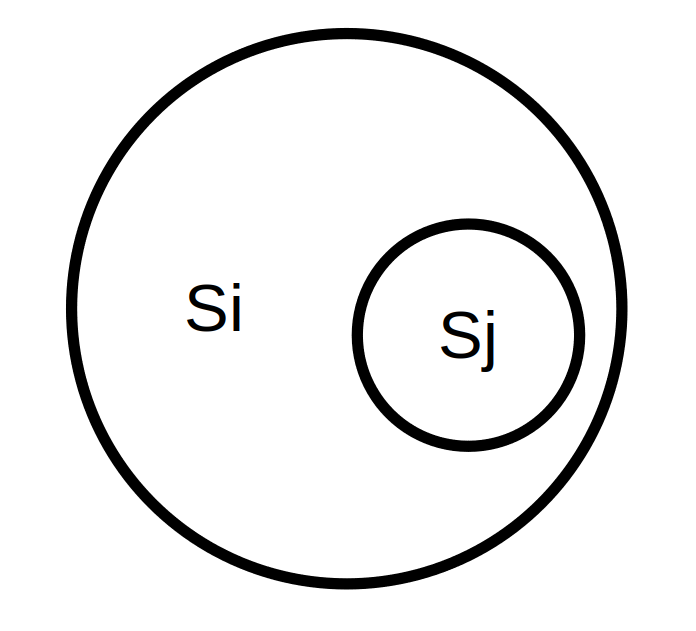
\includegraphics[scale=0.5]{images/fig_example.png}
	\label{fig:example}
\end{figure}

Рисунок \textit{\nameref{fig:example_scg}} показывает, как надо оформлять рисунки в SCg-коде. Параметр scale должен быть выставлен равным 0.8, для того чтобы все рисунки в SCg-коде имели одинаковый масштаб и размер идентификаторов примерно соответствовал размеру шрифта основного текста.  

\begin{figure}[H]
	\caption{SCg-текст. Пример рисунка в SCg-коде}
	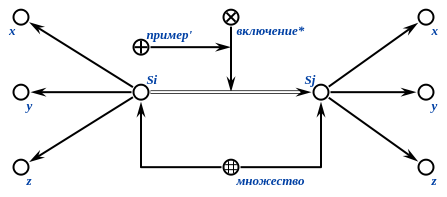
\includegraphics[scale=0.8]{images/fig_example_scg.png}
	\label{fig:example_scg}
\end{figure}


\section*{Правила оформления scn-текста}

Для оформления списков внутри естественно-языкового файла, находящегося в рамках формального sc.n-текста, то необходимо использовать
\begin{lstlisting}              
\begin{scnitemize}
	\item text
\end{scnitemize}
\end{lstlisting}  

Для оформления списков в рамках естественного-языкового текста (не SCn), то следует использовать:
\begin{lstlisting}              
\begin{textitemize}
	\item text
\end{textitemize}
\end{lstlisting}  

Использование \textbf{шрифтов}

\begin{lstlisting}
\underline{text} or \uline{text}
\textit{text}
\emph{text}
\textbf{text}
\textup{text}
\end{lstlisting}

Результат компиляции:

\underline{подчеркивание} или \uline{подчер\-кивание}

\textit{курсив}

\emph{выделенный шрифт}

\textbf{полужирный}

\textup{прямой шрифт}

Использование \textbf{символов}

\begin{lstlisting}
text\scnrolesign
text\textasciicircum
\end{lstlisting}

Результат компиляции:

	текст\scnrolesign
	
	текст\textasciicircum


Рассмотрим примерную структуру описания scn-конструкции. Пример исходного кода:

\begin{lstlisting}              
\begin{SCn}
	\scnheader{header}
	\scnidtftext{frequently used sc-identifier}{text}
	\scnidtf{text}
	\scniselement{text}
	\scnhaselement{text}
	\scnsuperset{text}
	\scnsubset{text}
	\scnidtfdef{text}
	\scndefinition{text}
	\scnidtfexp{text}
	\scnexplanation{text}
	\scntext{text}
	{Text
		\begin{textitemize}
			\item text;
			\item text
		\end{textitemize}
	}
	\scnnote{text}
	\scncomment{text}
	%dividing
	\begin{scnsubdividing}
		\scnitem{text}
		\scnitem{text}
		%nesting change
		\begin{scnindent}
			\scnidtf{text}
			\scneq{\textup{(} text \textup{)}}
			\begin{scneqtoset}
				\scnitem{text}
				\scnitem{text}
			\end{scneqtoset}
		\end{scnindent} 
	\end{scnsubdividing}
	\scnrelfrom{dividing}{attribute}
	\begin{scnindent}
		\begin{scneqtoset}
			\scnitem{text}
			\scnitem{text}
		\end{scneqtoset}
	\end{scnindent} 
	\begin{scnrelfromset}{relation}
		\scnitem{text}
		\scnitem{text}
	\end{scnrelfromset}
	\begin{scnrelfromset}{relation}
		\scnfileitem{text}
		\scnfileitem{text}
	\end{scnrelfromset}
	\begin{scnrelfromlist}{note}
		\scnfileitem{text}
		\scnfileitem{text}
	\end{scnrelfromlist}
	\scnrelboth{analog}{dividing*}
	\begin{scnrelfromlistcustom}{principles underlying}
		\scnitemcustom{text}
		\scnitemcustom{text}
	\end{scnrelfromlistcustom}
	\scnrelfrom{second domain}{text}
\end{SCn}
\end{lstlisting} 

Результат компиляции:
	\begin{SCn}
	\scnheader{ключевой sc-элемент}
	\scnidtftext{часто используемый sc-идентификатор}{text}
	\scnidtf{синонимичный идентификатор}
	\scniselement{принадлежность}
	\scnhaselement{принадлежность}
	\scnsuperset{строгое надмножество --- <<включает в себя>>}
	\scnsubset{cрогое подмножество --- <<включено в>>}
	\scnidtfdef{определение}
	\scndefinition{определение}
	\scnidtfexp{пояснение}
	\scnexplanation{пояснение}
	\scntext{пояснение}
	{Текст
		\begin{textitemize}
			\item текст;
			\item текст.
		\end{textitemize}
	}
	\scnnote{примечание}
	\scncomment{комментарий}
	%разбиение
	\begin{scnsubdividing}
		\scnitem{текст}
		\scnitem{текст}
		%изменение вложенности
		\begin{scnindent}
			\scnidtf{текст}
			\scneq{\textup{(} текст \textup{)}}
			\begin{scneqtoset}
				\scnitem{текст}
				\scnitem{текст}
			\end{scneqtoset}
		\end{scnindent} 
	\end{scnsubdividing}
	%отношение разбиение с признаком
	\scnrelfrom{разбиение}{Признак}
	\begin{scnindent}
		\begin{scneqtoset}
			\scnitem{текст}
			\scnitem{текст}
		\end{scneqtoset}
	\end{scnindent} 
	\begin{scnrelfromset}{отношение}
		\scnitem{текст}
		\scnitem{текст}
	\end{scnrelfromset}
	\begin{scnrelfromset}{отношение}
		\scnfileitem{текст}
		\scnfileitem{текст}
	\end{scnrelfromset}
	\begin{scnrelfromlist}{примечание}
		\scnfileitem{текст}
		\scnfileitem{текст}
	\end{scnrelfromlist}
	\scnrelboth{аналог}{разбиение*}
	\begin{scnrelfromlistcustom}{принципы, лежащие в основе}
		\scnitemcustom{текст}
		\scnitemcustom{текст}
	\end{scnrelfromlistcustom}
	\scnrelfrom{второй домен}{текст}
\end{SCn}

\begin{lstlisting}
\begin{SCn}
	\scnheader{relation*}
	\scnrelto{second domain}{text}
\end{SCn}
\end{lstlisting}

\begin{SCn}
	\scnheader{отношение*}
	\scnrelto{второй домен}{текст}
\end{SCn}

Результат компиляции:

текст\scnrolesign

текст\textasciicircum

Следует отличать:

\begin{lstlisting}
\begin{SCn}
	\scnheader{should be distinguished}
	\begin{scnhaselementset}
		\scnitem{text}
		\scnitem{text}
	\end{scnhaselementset}
\end{SCn}
\end{lstlisting}

В результате:

\begin{SCn}
	\scnheader{следует отличать}
	\begin{scnhaselementset}
		\scnitem{текст}
		\scnitem{текст}
	\end{scnhaselementset}
\end{SCn}
	
\newpage


\begin{partbacktext}
\part{Введение в интеллектуальные компьютерные системы нового поколения и технологию комплексной поддержки их жизненного цикла}
\label{part1}

\begin{SCn}
	\scntext{аннотация}{Уточнение понятия интеллектуальной компьютерной системы. Требования предъявляемые в интеллектуальным компьютерным системам следующего (нового) поколения и принципы, лежащие в их основе. Структура и особенности жизненного цикла интеллектуальных компьютерных систем нового поколения. Технология комплексной поддержки жизненного цикла интеллектуальных компьютерных систем нового поколения (\textit{Технология OSTIS} --- Open Semantic Technology for Intelligent Systems)}
	
	\bigskip
	
	\begin{scnrelfromlist}{подраздел}
		\scnitem{Глава~\ref{chap_intro}~\nameref{chap_intro}}
		\scnitem{Глава~\ref{chapter_new_generation_systems}~\nameref{chapter_new_generation_systems}}
		\scnitem{Глава~\ref{chapter_ostis_tech}~\nameref{chapter_ostis_tech}}
	\end{scnrelfromlist}
\end{SCn}

\end{partbacktext}

\chapter{Факторы, определяющие уровень интеллекта кибернетических систем}
\chapauthortoc{Загорский А.~С.\\Голенков В.~В.\\Шункевич Д.~В.}
{\label{chap_intro}}

\vspace{-7\baselineskip}

\begin{SCn}
\begin{scnrelfromlist}{автор}
	\scnitem{Загорский А.~Г.}
	\scnitem{Голенков В.~В.}
	\scnitem{Шункевич Д.~В.}
\end{scnrelfromlist}

\scntext{аннотация}{Рассмотрена иерархическая система свойств (в том числе способностей) \textit{кибернетических систем}, определяющих их качество и позволяющих сформулировать требования, которым должна удовлетворять \textit{высокоинтеллектуальная система} (кибернетическая система с сильным интеллектом).}

\begin{scnrelfromlist}{подраздел}
	\scnitem{\ref{sec_cyb_syst}~\nameref{sec_cyb_syst}}
	\scnitem{\ref{sec_mas}~\nameref{sec_mas}}
	\scnitem{\ref{sec_directions_evolution_computer_systems}~\nameref{sec_directions_evolution_computer_systems}}
\end{scnrelfromlist}

\end{SCn}

\section{Понятие интеллектуальной кибернетической системы}
{\label{sec_cyb_syst}} 

\begin{SCn}

\bigskip

\begin{scnrelfromlist}{ключевое понятие}
	\scnitem{кибернетическая система}
	\scnitem{качество кибернетических систем\scnsupergroupsign}
	\scnitem{уровень интеллекта кибернетических систем\scnsupergroupsign}
	\scnitem{интеллектуальная кибернетическая система}
\end{scnrelfromlist}

\bigskip

\begin{scnrelfromlist}{ключевое знание}
	\scnitem{Классификация кибернетических систем}
	\scnitem{Обобщенная архитектура кибернетических систем}
	\scnitem{Факторы, определяющие качество кибернетических систем}
	\scnitem{Факторы, определяющие уровень интеллекта кибернетических систем}
\end{scnrelfromlist}

\bigskip

\begin{scnrelfromlist}{библиографическая ссылка}
	\scnitem{\scncite{Glushkov1979}}
	\scnitem{\scncite{Varshavskiy1984}}
	\scnitem{\scncite{Finn2021}}
	\scnitem{\scncite{Nilsson2005}}
	\scnitem{\scncite{Kerr2006}}
	\scnitem{\scncite{Antsyferov2013}}
	\scnitem{\scncite{Fry2002}}
	\scnitem{\scncite{Melekhova2018}}
	\scnitem{\scncite{Ouksel1999}}
	\scnitem{\scncite{Lopes2022}}
	\scnitem{\scncite{Hamilton2006}}
	\scnitem{\scncite{Neiva2016}}
\end{scnrelfromlist}

\bigskip

\begin{scnrelfromlist}{подраздел}
	\scnitem{\ref{sec_cyb_syst_typology}~\nameref{sec_cyb_syst_typology}}
	\scnitem{\ref{sec_cyb_syst_structure}~\nameref{sec_cyb_syst_structure}}
	\scnitem{\ref{sec_cyb_syst_overall_quality}~\nameref{sec_cyb_syst_overall_quality}}
	\scnitem{\ref{sec_cyb_syst_physical_shell_quality}~\nameref{sec_cyb_syst_physical_shell_quality}}
	\scnitem{\ref{sec_cyb_syst_information_quality}~\nameref{sec_cyb_syst_information_quality}}
	\scnitem{\ref{sec_cyb_syst_problem_solver_quality}~\nameref{sec_cyb_syst_problem_solver_quality}}
	\scnitem{\ref{sec_cyb_syst_learnability_quality}~\nameref{sec_cyb_syst_learnability_quality}}
	\scnitem{\ref{sec_cyb_syst_intelligence_quality}~\nameref{sec_cyb_syst_intelligence_quality}}
\end{scnrelfromlist}

\end{SCn}

\bigskip

\subsection*{Введение в \ref{sec_cyb_syst}}

Кибернетическая система (см. \scncite{Glushkov1979}) есть cистема, которая способна управлять своими действиями, адаптируясь к изменениям состояния внешней среды (среды своего "обитания") в целях самосохранения (сохранения своей целостности и "комфортности"{} существования путем удержания своих "жизненно"{} важных параметров в определенных рамках "комфортности") и в целях формирования определенных реакций (воздействий на внешнюю среду) в ответ на определенные стимулы (на определенные ситуации или события во внешней среде), а также которая способна (при соответствующем уровне развития) эволюционировать в направлении:

\begin{textitemize}
    \item изучения своей внешней среды как минимум для предсказания последствий своих воздействий на внешнюю среду, а также для предсказания изменений внешней среды, которые не зависят от собственных воздействий;
    \item изучения самой себя и, в частности, своего взаимодействия с внешней средой;
    \item создания технологий (методов и средств), обеспечивающих изменение своей внешней среды (условий своего существования) в собственных интересах.
\end{textitemize}

\begin{SCn}
\scnheader{кибернетическая система}
\scnidtf{адаптивная система}
\scnidtf{целенаправленная система}
\scnidtf{активный субъект самостоятельной деятельности}
\scnidtf{материальная сущность, способная целенаправленно (в своих интересах) воздействовать на среду своего обитания как минимум для сохранения своей целостности, жизнеспособности, безопасности}
\scntext{примечание}{Уровень (степень) адаптивности, целенаправленности, активности у систем, основанных на обработке информации может быть самым различным.}
\scnidtf{система, организация функционирования которой основано на обработке информации о той среде, в которой существует эта система}
\scnidtf{материальная сущность, способная к активной  целенаправленной деятельности, которая  на определенном уровне развития указанной сущности становится "осмысленной", планируемой, преднамеренной деятельностью}
\scnidtf{субъект, способный на самостоятельное выполнение некоторых "внутренних"{} и "внешних"{} действий либо порученных извне, либо инициированных самим субъектом}
\scnidtf{сущность, способная выполнять роль субъекта деятельности}
\scnidtf{естественная или искусственно созданная система, способная мониторить и анализировать свое состояние и состояние окружающей среды, а также способная достаточно активно воздействовать на собственное состояние и на состояние окружающей среды}
\scnidtf{система, способная в достаточной степени самостоятельно взаимодействовать со своей средой, решая различные задачи}
\scnidtf{система, основанная на обработке информации}

\end{SCn}

Кибернетическая система динамически сопоставляет полученную информацию с выбранными действиями, относящимися к задаче, которая определяет основную цель системы \scncite{Fry2002}.

\input{author/part1/chapter_intro/cyb_syst_intelligence/typology.tex}
\input{author/part1/chapter_intro/cyb_syst_intelligence/structure.tex}
\input{author/part1/chapter_intro/cyb_syst_intelligence/overall_quality.tex}

\section{Понятие интеллектуальной многоагентной системы}
{\label{sec_mas}} 

\begin{SCn}

\bigskip

\begin{scnrelfromlist}{ключевое понятие}
    \scnitem{индивидуальная кибернетическая система}
    \scnitem{многоагентная система}
        \begin{scnindent}
        \scnsuperset{кибернетическая система} 
        \end{scnindent}
    \scnitem{иерархическая кибернетическая система}
    \scnitem{агент}
    \scnitem{многоагентная система}
        \begin{scnindent}
        \scnidtf{самостоятельный компонент многоагентной системы}
        \scnidtf{кибернетическая система, являющаяся агентом по крайней мере одной многоагентной системы}
        \end{scnindent}
    \scnitem{агент*}
        \begin{scnindent}
        \scnidtf{быть агентом заданной многоагентной системы*}
        \scnrelfrom{второй домен}{агент}
        \end{scnindent}
    \scnitem{индивидуальный агент}
    \scnitem{коллективный агент}
    \scnitem{встроенный агент}
        \begin{scnindent}
        \scnidtf{внутренний агент индивидуальной кибернетической системы}
        \end{scnindent}
    \scnitem{специализированный агент}
        \begin{scnindent}
        \scnidtf{интеллектуальный агент}
        \end{scnindent}
    \scnitem{мультиагент}
        \begin{scnindent}
        \scnidtf{кибернетическая система, являющаяся агентом более чем одной многоагентной системы}
        \end{scnindent}
\end{scnrelfromlist}

\bigskip
    
\begin{scnrelfromlist}{ключевое знание}
    \scnitem{Классификация многоагентных систем} 
    \scnitem{Обобщенная архитектура кибернетических систем} 
    \scnitem{Факторы, определяющие качество многоагентных систем}
    \scnitem{Факторы, определяющие уровень интеллекта многоагентных систем}
\end{scnrelfromlist}

\bigskip

\begin{scnrelfromlist}{рассматриваемый вопрос}
    \scnitem{Почему переход от отдельных \textit{кибернетических систем} к их коллективным, многоагентным системам, агентами которых являются заданные \textit{кибернетические системы}, является одним из направлений повышения уровня интеллекта исходных \textit{кибернетических систем}.}
    \scnitem{Всегда ли объединение кибернетических систем в коллектив этих систем приводит у повышению уровня интеллекта.}
    \scnitem{Почему не каждое соединение достаточно качественных \textit{кибернетических систем} порождает качественную многоагентную систему.}
\end{scnrelfromlist}

\bigskip

\begin{scnrelfromlist}{библиографическая ссылка}
    \scnitem{\scncite{Tarasov2002}}
    \scnitem{\scncite{Varshavskiy1984}}
    \scnitem{\scncite{Hadzic2009}}
    \scnitem{\scncite{Dorri2018}}
    \scnitem{\scncite{Ferber2003}}
    \scnitem{\scncite{Balaji2010}}
\end{scnrelfromlist}

\end{SCn}

\bigskip

Переход от кибернетических систем к коллективам взаимодействующих между собой кибернетических систем, то есть к социальной организации кибернетических систем, является важнейшим фактором эволюции кибернетических систем. 
Кибернетическую систему, представляющую собой коллектив взаимодействующих кибернетических систем, обладающих определенной степенью самостоятельности (самодостаточности, свободы выбора), будем называть многоагентной системой \scncite{Dorri2018}.

\begin{SCn}
\scnheader{кибернетическая система}
\begin{scnrelfromset}{разбиение}
    \scnitem{индивидуальная кибернетическая система}
    \scnitem{кибернетическая система, являющаяся минимальным компонентом индивидуальной кибернетической системы}
    \scnitem{кибернетическая система, являющаяся комплексом компонентов соответствующей индивидуальной кибернетической системы}
    \scnitem{сообщество индивидуальных кибернетических систем}
    \begin{scnindent}
    \begin{scnrelfromset}{разбиение}
        \scnitem{простое сообщество индивидуальных кибернетических систем}
        \scnitem{иерархическое сообщество индивидуальных кибернетических систем}
    \end{scnrelfromset}
    \end{scnindent}
\end{scnrelfromset}
\end{SCn}

\begin{SCn}
	\scnheader{Теория многоагентных систем}
	\scnexplanation{Теория многоагентных систем --- это теория перехода количества кибернетических систем  в кибернетическую систему нового качества, --- это выявление принципов и методов, позволяющие множество кибернетических систем соединить в коллективную кибернетическую систему, обладающую существенно более высоким уровнем качества (в том числе интеллекта) по сравнению с качеством кибернетической системы, входящих в этот коллектив}
\end{SCn}


Агенты многоагентной системы могут (но вовсе не обязательно должны) быть интеллектуальными системами. 
Так, например, агенты интеллектуального решателя задач, имеющего агентно-ориентированную архитектуру, не являются интеллектуальными системами. 
Агентом иерархической многоагентной системы может быть другая многоагентная система \scncite{Ferber2003}.

Многоагентная система есть коллектив взаимодействующих автономных кибернетических систем, имеющих общую среду обитания, жизнедеятельности \scncite{Hadzic2009}. 

Классификация многоагентных систем приведена ниже:

\begin{SCn}
\scnheader{многоагентная система}
\begin{scnrelfromset}{разбиение}
    \scnitem{одноуровневая многоагентная система}
    \scnitem{иерархическая многоагентная система}
\end{scnrelfromset}
\end{SCn}

Одноуровневая многоагентная система реализует либо одну модель параллельного (распределенного) решения задач соответствующего класса, либо комбинацию фиксированного числа разных и параллельно реализованных моделей решения задач. 
Иерархическая многоагентная система состоит из агентов, которые могут быть индивидуальными кибернетическими системами, коллективами индивидуальных кибернетических систем, а также коллективами, состоящими из индивидуальных кибернетических систем и коллективов индивидуальных кибернетических систем.

В многоагентной системе с централизованным управлением специально выделяются агенты, которые принимают решения в определенной области деятельности многоагентной системы и обеспечивают выполнение этих решений путем управления деятельностью остальных агентов, входящих в состав этой системы.

В многоагентной системе с децентрализованным управлением решения принимаются коллегиально и "автоматически"{} (решения о признании новой кем-то предложенной информации – в том числе, об инициировании некоторой задачи, решения о коррекции (уточнении) уже ранее признанной, согласованной информации) на основе четко продуманной и постоянно совершенствуемой методики, а также на основе активного участия всех агентов в формировании новых предложений, подлежащих признанию или согласованию \scncite{Balaji2010}. 
В такой многоагентной системе все агенты участвуют в управлении этой системы. 
Примером такой системы является оркестр, способный играть без дирижера.

\input{author/part1/chapter_intro/mas_intelligence/overall_quality.tex}


\section{Направления эволюции компьютерных систем}
\label{sec_directions_evolution_computer_systems}
В эволюции компьютерных систем можно выделить два общих направления.

\textbf{Первое направление} --- это 
\begin{textitemize}
	\item \textbf{расширение множества и многообразия задач}, решаемых компьютерной системой; 
	\item повышение \textbf{сложности этих задач} вплоть до трудно формализуемых (трудно решаемых) задач, интеллектуальных задач, решаемых в условиях неполноты, неточности, нечеткости и так далее;
	\item повышение \textbf{качества решения задач} либо путем более эффективного использования известных моделей решения задач (например, путем разработки более качественных алгоритмов), либо путем использования принципиально новых моделей решения задач;
	\item расширение \textbf{многообразия используемых видов информации} (знаний);
	\item расширение \textbf{многообразия используемых моделей решения задач}.
\end{textitemize}

Очевидно, что расширение множества решаемых задач в условиях пусть и большой, но всегда конечной памяти компьютерной системы делает все более и более актуальным переход от частных методов и моделей решения задач к их обобщениям (или, как отмечал Д.~А. Поспелов, от связки "ключей"\ к набору "отмычек").

Очевидно также, что многообразие видов задач, решаемых компьютерными системами, многообразие используемых моделей решения задач приводит: 
\begin{textitemize}
	\item к интегрированным информационным ресурсам;
	\item к интегрированным решателям задач;
	\item к интегрированным компьютерным системам;
	\item к коллективам компьютерных систем.
\end{textitemize}

Проблема здесь заключается не в самой интеграции, а в ее качестве. Интеграция может быть \textbf{эклектичной}, если не обеспечить совместимость интегрируемых компонентов, а в случае такой совместимости интеграция может привести к новому качеству, к дополнительному расширению множества решаемых задач. Это будет означать переход от эклектичности к гибридности, синергетичности.

\textbf{Второе общее направление} эволюции компьютерных систем --- это повышение уровня их \textbf{обучаемости} и, как следствие, темпов их эволюции.

\textbf{Обучаемость} компьютерной системы определяется:
\begin{textitemize}
	\item \textbf{трудоемкостью} и темпами приобретения (расширения) и совершенствования активно используемых знаний и навыков;
	\item \textbf{уровнем ограничений}, накладываемых на вид приобретаемых и используемых знаний и навыков (фактически, это ограничения на множество всех тех задач, которые принципиально могут быть решены данной компьютерной системой).
\end{textitemize}

В свою очередь, \textbf{трудоемкость и темпы расширения и совершенствования} знаний и навыков компьютерной системы определяется:
\begin{textitemize}
	\item \textbf{гибкостью} --- многообразием и трудоемкостью возможных изменений, вносимых в систему в процессе пополнения системы новыми знаниями и навыками и совершенствования уже приобретенных знаний и навыков;
	\item \textbf{стратифицированностью} --- четким разделением системы на достаточно независящие друг от друга уровни иерархии, то есть возможностью локализации фрагментов компьютерной системы, не выходя за пределы которых, \myuline{априори достаточно} проводить анализ последствий тех или иных вносимых в систему изменений;
	\item \textbf{рефлексивностью} --- способностью анализировать собственное состояние и свою деятельность;
	\item \textbf{гибридностью} --- способностью приобретать и использовать широкое (а в идеале --- неограниченное) многообразие знаний и навыков;
	\item \textbf{уровнем самообучаемости} --- уровнем активности, самостоятельности, целеустремленности в процессе своего обучения, то есть уровнем способности к обучению \myuline{без учителя}, уровнем автоматизации приобретения новых знаний и навыков, а также совершенствования уже приобретенных знаний и навыков;
	\item \textbf{совместимостью} --- трудоемкостью интеграции;
	\item \textbf{способностью к постоянному мониторингу и поддержке своей совместимости} как с другими компьютерными системами, так и со своими пользователями в условиях интенсивной эволюции этих компьютерных систем и их пользователей. 
\end{textitemize}

\textbf{Совместимость} (трудоемкость интеграции) компьютерных систем может рассматриваться в двух аспектах:
\begin{textitemize}
	\item в аспекте \textbf{глубокой интеграции} компьютерных систем, что предполагает преобразование нескольких компьютерных систем в одну целостную компьютерную систему путем объединения информационных и функциональных ресурсов интегрируемых компьютерных систем;
	\item в аспекте преобразования нескольких компьютерных систем в \textbf{коллектив взаимодействующих компьютерных систем}, способных к совместному корпоративному решению сложных задач.
\end{textitemize}

Совместимость (трудоемкость интеграции) компьютерных систем определяется:
\begin{textitemize}
	\item совместимостью различного вида информации (знаний), хранимой в памяти компьютерной системы;
	\item совместимостью различных моделей решения задач;
	\item совместимостью встроенных (в том числе типовых) подсистем, входящих в состав компьютерных систем;
	\item совместимостью внешней информации, поступающей на вход компьютерной системе, с информацией, хранимой в памяти компьютерной системы (трудоемкостью понимания внешней информации --- трансляции, погружения, выравнивания понятий);
	\item коммуникационной (в том числе семантической) совместимостью с пользователями и с другими компьютерными системами.
\end{textitemize}

Важнейшая форма обучения компьютерной системы это приобретение новых знаний и навыков в "готовом"\ виде, то есть в виде некоторых знаковых конструкций, вводимых в память компьютерной системы, поскольку приобретение знаний и навыков из внешних достоверных источников требует существенно меньшего времени по сравнению с их приобретением собственными силами, на основе собственного опыта и собственных ошибок. Но для того, чтобы указанная форма обучения была эффективной, необходимо максимально возможным образом упростить и формализовать механизм (процедуру) погружения новых знаний в память компьютерной системы.

Для решения этой задачи ключевое значение имеет создание удобного для этой цели способа кодирования различного вида информации в памяти компьютерной системы.

Поскольку основным каналом обучения компьютерных систем является приобретение ими знаний и навыков от других субъектов --- от других компьютерных систем и от пользователей (от разработчиков-учителей и от конечных пользователей), важнейшим фактором обучаемости компьютерной системы является превращение компьютерной системы в коммуникативную систему, способную эффективно общаться с внешними субъектами. Следовательно, уровень обучаемости компьютерных систем определяется также уровнем ее совместимости с самими этими внешними субъектами, с приобретаемыми ею знаниями и навыками, то есть степенью того, как компьютерная система вместе с теми субъектами, с которыми она обменивается информацией, решает проблему "вавилонского столпотворения"{}.

% \input{author/references}
\chapauthor{Голенков В.В.\\Шункевич Д.В.\\Ковалёв М.В.\\Садовский М.Е.}
\chapter{Интеллектуальные компьютерные системы нового поколения}
\chapauthortoc{Голенков В.В.\\Шункевич Д.В.\\Ковалёв М.В.\\Садовский М.Е.}
\label{chapter_new_generation_systems} 

\abstract{Аннотация к главе.}

\section{Введение}

Важнейшим направлением повышения уровня \textit{интеллекта} \textit{индивидуальных интеллектуальных кибернетических систем} является переход к \textit{коллективам индивидуальных интеллектуальных кибернетических систем} и далее к \textit{иерархическим коллективам интеллектуальных кибернетических систем}, членами которых являются как \textit{индивидуальные интеллектуальные кибернетические системы}, так и \textit{коллективы индивидуальных интеллектуальных кибернетических систем}, а также \textit{иерархические коллективы интеллектуальных кибернетических систем}. 

Аналогичным образом необходимо повышать уровень интеллекта и \textit{индивидуальных интеллектуальных \underline{компьютерных} систем} (искусственных \textit{кибернетических систем}). Но при этом надо помнить, что далеко не каждое объединение \textit{\underline{интеллектуальных} кибернетических систем} (в том числе и \textit{компьютерных систем}) становится \textit{интеллектуальным коллективом}. Для этого необходимо соблюдение дополнительных требований, предъявляемых \underline{ко всем} членам \textit{интеллектуальных коллективов}. Важнейшим из них является требование высокого уровня \textbf{\textit{интероперабельности}}, т.е. способности к эффективному взаимодействию с другими членами коллектива. Переход от современных \textit{интеллектуальных компьютерных систем} к \textit{интероперабельным интеллектуальным компьютерным системам} является ключевым фактором перехода к \textbf{\textit{интеллектуальным компьютерным системам нового поколения}}, обеспечивающим существенное повышение уровня автоматизации человеческой деятельности.

\section{Требования, предъявляемые к интеллектуальным компьютерным системам нового поколения}

Создание различных комплексов взаимодействующих \textit{интеллектуальных компьютерных систем} \underline{требует} повышения качества не только самих этих систем, но также и качества их взаимодействия. \textit{Интеллектуальные компьютерные системы нового поколения} должны иметь высокий уровень \textbf{\textit{интероперабельности}}, то есть высокий уровень способности к эффективному, целенаправленному взаимодействию с себе подобными и с пользователями в процессе коллективного (распределённого) и децентрализованного решения сложных задач \cite{Yaghoobirafi2022,Ouksel1999,Lanzenberger2008,Neiva2016,Pohl2004,Waters2009}. Уровень \textbf{\textit{интероперабельности}} \textit{интеллектуальных компьютерных систем} -- это, образно говоря, уровень их "социализации"{}, полезности в рамках различных априори неизвестных сообществ (коллективов) \textit{интеллектуальных систем}.

Уровень \textbf{\textit{интероперабельности}} \textit{интеллектуальных компьютерных систем} -- это уровень их коммуникационной (социальной) совместимости, позволяющей им \underline{самостоятельно} формировать коллективы \textit{интеллектуальных компьютерных систем} и их пользователей, а также \underline{самостоятельно} согласовывать и координировать свою деятельность в рамках этих коллективов при решении сложных задач в частично предсказуемых условиях. Повышение уровня \textit{интероперабельности} интеллектуальных компьютерных систем определяет переход к \textbf{\textit{интеллектуальным компьютерным системам нового поколения}}, без которых невозможна реализация таких проектов, как smart-предприятие, smart-больница, smart-город, smart-общество \cite{Lopes2022,Hamilton2006}.

\begin{SCn}
	\scnheader{интеллектуальная компьютерная система}
	\scnidtf{интеллектуальная искусственная кибернетическая система}
	\begin{scnrelfromset}{разбиение}
		\scnitem{индивидуальная интеллектуальная компьютерная система}
		\scnitem{интеллектуальный коллектив интеллектуальных компьютерных систем}
		\begin{scnindent}
			\scnidtf{интеллектуальная \textit{многоагентная система}, агенты которой являются \textit{интеллектуальными компьютерными системами}}
			\scntext{примечание}{Не каждый \textit{коллектив интеллектуальных компьютерных систем} может оказаться интеллектуальным, поскольку уровень интеллекта такого коллектива определяется не только уровнем интеллекта его членов, но также и эффективностью (качеством) \underline{их взаимодействия}.}
			\begin{scnrelfromset}{разбиение}
				\scnitem{интеллектуальный коллектив \underline{индивидуальных} интеллектуальных компьютерных систем}
				\scnitem{иерархический интеллектуальный коллектив интеллектуальных компьютерных систем}
				\begin{scnindent}
					\scnidtf{\textit{интеллектуальный коллектив интеллектуальных компьютерных систем}, по крайней мере одним из членов которого является \textit{интеллектуальный коллектив интеллектуальных компьютерных систем}}
				\end{scnindent}
			\end{scnrelfromset}
		\end{scnindent}
	\end{scnrelfromset}
\end{SCn}

\begin{SCn}
	\scnheader{интеллектуальные компьютерные системы нового поколения}
	\begin{scnrelfromlistcustom}{предъявляемые требования}
		\scnitemcustom{высокий уровень \textit{интероперабельности}}
		\scnitemcustom{высокий уровень \textit{обучаемости}}
		\scnitemcustom{высокий уровень \textit{гибридности}}
		\scnitemcustom{высокий уровень способности решать \textit{интеллектуальные задачи} (то есть \textit{задачи}, \textit{методы} решения которых и/или требуемая для их решения исходная информация априори неизвестны)}
		\scnitemcustom{высокий уровень \textit{синергетичности}}
	\end{scnrelfromlistcustom}
	
	\scnheader{интероперабельность\scnsupergroupsign}
	\scnidtf{способность к эффективному (целенаправленному) взаимодействию с другими самостоятельными субъектами}
	\scnidtf{способность к партнёрскому взаимодействию в решении \textit{комплексных задач}, требующих \textit{коллективной деятельности}}
	\scnidtf{способность работать в коллективе (в команде)}
	\scnidtf{уровень социализации}
	\scnidtf{social skills}
	
	\scnheader{высокий уровень интероперабельности}
	\begin{scnrelfromlistcustom}{обеспечивается}
		\scnitemcustom{высоким уровнем \textit{взаимопонимания}}
		\begin{scnindent}
			\begin{scnrelfromlistcustom}{обеспечивается}
				\scnitemcustom{высоким уровнем \textbf{\textit{семантической совместимости}} заданного субъекта с другими субъектами заданного коллектива}
				\scnitemcustom{высоким уровнем \textit{способности понимать} сообщения и поведение партнеров}
				\scnitemcustom{высоким уровнем \textit{способности быть понятной} для партнеров:
					\begin{itemize}
						\item[--] способности понятно и обоснованно формулировать свои предложения и информацию, полезную для решения текущих задач;
						\item[--] способности действовать и комментировать свои действия так, чтобы они и их мотивы были понятны партнерам;
				\end{itemize}}
				
				\scnitemcustom{высоким уровнем \textit{способности к повышению уровня семантической совместимости} со своими партнёрами}
			\end{scnrelfromlistcustom}
		\end{scnindent}
		\scnitemcustom{высоким уровнем \textit{договороспособности}, то есть способности согласовывать с партнёрами свои планы и намерения в целях своевременного обеспечения высокого качества коллективного результата}
		\scnitemcustom{высоким уровнем \textit{способности к децентрализованной координации} своих действий с действиями партнёров в непредсказуемых (нештатных) обстоятельствах}
		\scnitemcustom{высоким уровнем \textit{способности к минимизации негативных последствий конфликтных ситуаций} с другими субъектами}
		\begin{scnindent}
			\begin{scnrelfromlistcustom}{обеспечивается}
				\scnitemcustom{высоким уровнем \textit{способности к предотвращению возникновения конфликтных ситуаций}}
				\scnitemcustom{\textit{соблюдением этических норм} и правил, препятствующих возникновению разрушительных последствий конфликтных ситуаций}
				\scnitemcustom{высоким уровнем \textit{способности разделять ответственность} с партнерами за своевременное и качественное достижение общей цели}
			\end{scnrelfromlistcustom}
		\end{scnindent}
	\end{scnrelfromlistcustom}
	
	\scnheader{семантическая совместимость\scnsupergroupsign}
	\scnidtf{степень согласованности (совпадения) систем \textit{понятий} и других \textit{ключевых сущностей}, используемых заданными взаимодействующими субъектами}
	\scntext{примечание}{Обеспечение \textit{семантической совместимости} требует формализации \textit{смыслового представления информации}}
\end{SCn}

\noindent
\textbf{\textit{способность разделять ответственность}} с партнерами, являющаяся необходимым условием децентрализованного управления коллективной деятельностью
\begin{SCn}
	\begin{scnrelfromlistcustom}{обеспечивается}
		\scnitemcustom{\textit{способностью к мониторингу} и анализу коллективно выполняемой деятельности}
		\scnitemcustom{\textit{способностью оперативно информировать партнеров} о неблагоприятных ситуациях, событиях, тенденциях, а также инициировать соответствующие коллективные действия}
	\end{scnrelfromlistcustom}
	
	\scnheader{обучаемость\scnsupergroupsign}
	\scnidtf{способность быстро и качественно приобретать новые \textit{знания} и \textit{навыки}, а также совершенствовать уже приобретённые \textit{знания} и \textit{навыки}}
	
	\scnheader{высокий уровень обучаемости}
	
	\begin{scnrelfromlistcustom}{обеспечивается}
		\scnitemcustom{высоким уровнем \textit{гибкости информации}, хранимой в памяти интеллектуальной системы}
		\scnitemcustom{высоким уровнем \textit{качества} \textit{стратификации информации}, хранимой в памяти интеллектуальной системы (стратифицированностью \textit{базы знаний}}
		\scnitemcustom{высоким уровнем \textit{рефлексивности} интеллектуальной системы}
		\scnitemcustom{высоким уровнем \textit{способности исправлять свои ошибки} (в том числе устранять противоречия в своей \textit{базе знаний})}
		\scnitemcustom{высоким уровнем \textit{познавательной активности}}
		\scnitemcustom{отсутствием \textit{ограничений на вид приобретаемых знаний и навыков} (отсутствие таких ограничений означает потенциальную \textit{универсальность} интеллектуальной системы)}
	\end{scnrelfromlistcustom}
	
	\scnheader{гибридность\scnsupergroupsign}
	\scnidtf{степень многообразия используемых \textit{видов знаний} и \textit{моделей решения задач} и уровень эффективности их совместного использования}
	\scnidtf{индивидуальная способность решать \textit{комплексные задачи}, требующие использования различных \textit{видов знаний}, а также различных комбинаций различных \textit{моделей решения задач}}
	
	\scnheader{высокий уровень гибридности}
	\begin{scnrelfromlistcustom}{обеспечивается}
		\scnitemcustom{высокой степенью многообразия используемых \textit{видов знаний} и \textit{моделей решения задач}}
		\scnitemcustom{высокой степенью \textit{конвергенции} и глубокой \textit{интеграции} (степенью взаимопроникновения) различных \textit{видов знаний} и \textit{моделей решения задач}}
		\scnitemcustom{способностью неограниченно расширять уровень своей \textit{гибридности}}
	\end{scnrelfromlistcustom}
\end{SCn}

Подчеркнем, что \textit{гибридность} и \textit{интероперабельность} \textit{интеллектуальных компьютерных систем нового поколения} предполагает отказ от известной парадигмы "черных ящиков"{}, поскольку:

\begin{itemize}
	\item
	всё многообразие моделей решения задач \textit{гибридной интеллектуальной компьютерной системы} должно интерпретироваться на одной общей \textit{универсальной платформе};
	\item
	доступность информации о том, как устроен каждый используемый метод, модель решения задач, каждый субъект существенно повышает качество их \textit{координации} при \textit{совместном решении комплексных задач};
	\item
	появляется возможность некоторые методы, модели решения задач и целые субъекты (например, \textit{интеллектуальные компьютерные системы}) использовать для совершенствования (повышения качества) других методов, моделей и субъектов.
\end{itemize}

Особо необходимо отметить следующие характеристики \textit{интеллектуальных компьютерных систем нового поколения}:
\begin{itemize}
	\item \textbf{\textit{степень}} \textbf{\textit{конвергенции}}, унификации и стандартизации \textit{интеллектуальных компьютерных систем} и их компонентов и соответствующая этому \textbf{\textit{степень интеграции}} (глубина интеграции) \textit{интеллектуальных компьютерных систем} и их компонентов;
	\item \textbf{\textit{семантическая совместимость}} между \textit{интеллектуальными компьютерными системами} в целом и \textit{семантическая совместимость} между компонентами каждой \textit{интеллектуальной компьютерной системы} (в частности, совместимость между различными \textit{видами знаний} и различными \textit{моделями обработки знаний}), которые являются основными показателями степени \textbf{\textit{конвергенции}} (сближения) между \textit{интеллектуальными компьютерными системами} и их компонентами.
\end{itemize}

Особенность указанных характеристик \textit{интеллектуальных компьютерных систем} их компонентов заключается в том, что они играют важную роль при решении всех ключевых задач современного этапа развития \textit{Искусственного интеллекта} и тесно связаны друг с другом.

Заметим также, что перечисленные требования, предъявляемые к \textit{интеллектуальным компьютерным системам нового поколения}, направлены на преодоление проклятия \textit{Вавилонского столпотворения}\cite{Illiadis2019} как внутри \textit{интеллектуальных компьютерных систем нового поколения} (между внутренними \textit{информационными процессами} решения различных задач), так и между взаимодействующими самостоятельными \textit{интеллектуальными компьютерными системами нового поколения} в процессе коллективного решения \textit{комплексных задач}.

На современном этапе эволюции \textit{интеллектуальных компьютерных систем} для существенного расширения областей их применения и качественного повышения уровня автоматизации человеческой деятельности:
\begin{itemize}
	\item
	Необходим переход к созданию \underline{семантически} \underline{совместимых} \textbf{\textit{интеллектуальных компьютерных систем \underline{нового поколения}}}, ориентированных не только на индивидуальное, но и на \underline{коллективное} (совместное) решение \textit{комплексных задач}, требующих скоординированной деятельности нескольких самостоятельных интеллектуальных компьютерных систем и использования различных моделей и методов в непредсказуемых комбинациях, что необходимо для существенного расширения сфер применения \textit{интеллектуальных компьютерных систем}, для перехода от автоматизации локальных видов и областей \textit{человеческой деятельности} к комплексной автоматизации более крупных (объединённых) видов и областей этой деятельности;
	\item
	Необходима разработка \textbf{\textit{Общей формальной теории и стандарта интеллектуальных компьютерных систем нового поколения}};
	\item
	Необходима разработка \textbf{\textit{Технологии комплексной поддержки жизненного цикла интеллектуальных компьютерных систем нового поколения}}, которая включает в себя поддержку \textit{проектирования} этих систем (как начального этапа их жизненного цикла) и обеспечение их \textit{совместимости} на всех этапах их жизненного цикла;
	\item
	Необходима \textbf{\textit{конвергенция}} и \textbf{\textit{унификация}} \textit{интеллектуальных компьютерных систем нового поколения} и их компонентов;
	\item
	Необходима реализация "бесшовной"{}, "диффузной"{}, взаимопроникающей, \textbf{\textit{глубокой интеграции семантически смежных компонентов интеллектуальных компьютерных систем}}, то есть интеграции, при которой отсутствуют чёткие границы ("швы") интегрируемых (соединяемых) компонентов, и которая может осуществляться \underline{автоматически}. Это означает переход к \textbf{\textit{\underline{гибридным} интеллектуальным компьютерным системам}};
	\item
	Необходимо соблюдение \textbf{\textit{Принципа бритвы Оккама}} -- максимально возможное структурное упрощение \textit{интеллектуальных компьютерных систем нового поколения}, исключение \underline{эклектичных} решений;
	\item
	Необходима ориентация на потенциально \textbf{\textit{универсальные}} (то есть способные быстро приобретать \underline{любые} знания и навыки), \textbf{\textit{синергетические}} \textit{интеллектуальные компьютерные системы} с "сильным"{} интеллектом;
\end{itemize}

\begin{SCn}
	\scnheader{интеллектуальные компьютерные системы нового поколения}
	\begin{scnrelfromlistcustom}{принципы, лежащие в основе}
		\scnitemcustom{\textit{смысловое представление знаний} в памяти \textit{интеллектуальных компьютерных систем}, предполагающее отсутствие \textit{омонимических знаков}, которые в разных контекстах обозначают разные сущности, а также отсутствие \textit{синонимии}, т.е. пар синонимичных \textit{знаков}, которые обозначают одну и ту же сущность. Смысловое представление информационной конструкции в общем случае имеет нелинейный (графовый) характер и называется \textit{семантической сетью}}
		\scnitemcustom{использование \underline{общего} для всех интеллектуальных компьютерных систем \textit{универсального языка смыслового представления знаний} в памяти \textit{интеллектуальных компьютерных систем}, обладающий максимально простым \textit{синтаксисом}, обеспечивающий представление любых \textit{видов знаний} и имеющий неограниченные возможности перехода от \textit{знаний} к \textit{метазнаниям}. Простота синтаксиса \textit{информационных конструкций} указанного \textit{языка} позволяет называть эти конструкции \textit{рафинированными семантическими сетями}}
		\scnitemcustom{\textit{структурно-перестраиваемая (графодинамическая) организация памяти} интеллектуальных компьютерных систем, при которой обработка знаний сводится не столько к изменению состояния хранимых \textit{знаков}, сколько к изменению конфигурации связей между этими \textit{знаками}}
		\scnitemcustom{\textit{семантически неограниченный ассоциативный доступ к информации}, хранимой в памяти \textit{интеллектуальных компьютерных систем}, по заданному образцу произвольного размера и произвольной конфигурации}
		\scnitemcustom{\textit{децентрализованное ситуационное управление информационными процессами} в памяти \textit{интеллектуальных компьютерных систем}, реализованное с помощью \textit{агентно-ориентированной модели обработки баз знаний}, в котором \textit{инициирование} новых \textit{информационных процессов} осуществляется не путём передачи управления соответствующим априори известным процедурам, а в результате возникновения соответствующих \textit{ситуаций} или \textit{событий} \textit{в памяти интеллектуальной компьютерной системы}, поскольку <<Основная проблема компьютерных систем состоит не в накоплении знаний, в умении активизировать нужные знания в процессе решения задач>> (Поспелов Д.А.). Такой многоагентный процесс обработки информации представляет собой \textit{деятельность}, выполняемую некоторым коллективом \underline{самостоятельных} \textit{информационных агентов} (агентов обработки информации), условием инициирования каждого из которых является появление в текущем состоянии \textit{базы знаний} соответствующей этому агенту \textit{ситуации} и/или \textit{события}.
			
			<<Выбор многоагентных технологий объясняется тем, что в настоящее время любая сложная производственная, логистическая или другая система может быть представлена набором взаимодействий более простых систем до любого уровня детальности, что обеспечивает фрактально-рекурсивный принцип построения многоярусных систем, построенных как открытые цифровые колонии и экосистемы ИИ. В основе многоагентных технологий лежит распределенный или децентрализованный подход к решению задач, при котором динамически обновляющаяся информация в распределенной сети интеллектуальных агентов обрабатывается непосредственно у агентов вместе с локально доступной информацией от "соседей"{}. При этом существенно сокращаются как ресурсные и временные затраты на коммуникации в сети, так и время на обработку и принятие решений в центре системы (если он все-таки есть).>>
		}
		\scnrelto{цитата}{Баринов И.И.. ФормиСРКпИИ-2021ст/с. 270 \cite{Barinov2021}}
		\scnitemcustom{Переход к \textit{семантическим} \textit{моделям решения задач}, в основе которых лежит учёт не только синтаксических (структурных) аспектов обрабатываемой информации, но также и \underline{семантических} (смысловых) аспектов этой информации -- ``From data science to knowledge science''}
		\scnitemcustom{\textbf{\textit{онтологическая модель баз знаний}} \textit{интеллектуальных компьютерных систем}, т.е. онтологическая структуризация всей информации, хранимой в памяти \textit{интеллектуальной компьютерной системы}, предполагающая четкую \textit{стратификацию базы знаний} в виде иерархической системы \textit{предметных областей} и соответствующих им \textit{онтологий}, каждая из которых обеспечивает семантическую \textit{спецификацию} всех \textit{понятий}, являющихся ключевыми в рамках соответствующей \textit{предметной области}}
		\scnitemcustom{\textbf{\textit{онтологическая локализация решения задач}} в \textit{интеллектуальных компьютерных системах}, предполагающая \underline{локализацию} \textit{области действия} каждого хранимого в памяти \textit{метода} и каждого \textit{информационного агента} в соответствии с \textit{онтологической моделью} обрабатываемой \textit{базы знаний}. Чаще всего, такой \textit{областью действия} является одна из \textit{предметных областей} либо одна из \textit{предметных областей} вместе с соответствующей ей \textit{онтологии}}
		\scnitemcustom{\textbf{\textit{онтологическая модель интерфейса}} \textit{интеллектуальной компьютерной системы,} в состав которой входит:
			\begin{itemize}
				\item[--] онтологическое описание \textit{синтаксиса} всех \textit{языков}, используемых \textit{интеллектуальной компьютерной системой} для \textit{общения} с внешними \textit{субъектами};
				\item[--] онтологическое описание \textit{денотационной семантики} каждого \textit{языка}, используемого \textit{интеллектуальной компьютерной системой} для \textit{общения} с внешними \textit{субъектами};
				\item[--] семейство \textit{информационных агентов}, обеспечивающих \textit{синтаксический анализ}, \textit{семантический анализ} (перевод на внутренний смысловой язык) и \textit{понимание} (погружение в \textit{базу знаний}) любого введенного \textit{сообщения}, принадлежащего любому \textit{внешнему языку}, полное онтологическое описание которого находится в базе знаний \textit{интеллектуальной компьютерной системы};
				\item[--] семейство \textit{информационных агентов}, обеспечивающих \textit{синтез сообщений}, которые (1) адресуются внешним субъектам, с которыми общается \textit{интеллектуальная компьютерная система}, (2) \textit{семантически эквивалентны} заданным \textit{фрагментам базы знаний} интеллектуальной компьютерной системы, определяющим \textit{смысл} передаваемых \textit{сообщений}, (3) принадлежат одному из \textit{внешних языков}, полное онтологическое описание которого находится в \textit{базе знаний} интеллектуальной компьютерной системы; 
			\end{itemize}
		}
		
		\scnitemcustom{\textit{семантически дружественный характер пользовательского интерфейса}, обеспечиваемый (1) формальным описание в базе знаний средства управления пользовательским интерфейсом и (2) введением в состав \textit{интеллектуальной компьютерной системы} соответствующих help-подсистем, обеспечивающих существенное снижение языкового барьера между пользователями и \textit{интеллектуальными компьютерными системами}, что существенно повысит эффективность \textit{эксплуатации интеллектуальных компьютерных систем}}
		\scnitemcustom{\textit{минимизация негативного влияния человеческого фактора} на эффективность \textit{эксплуатации} \textit{интеллектуальных компьютерных систем} благодаря реализации интероперабельного (партнерского) стиля взаимодействия не только между самими \textit{интеллектуальными компьютерными системами}, но также и между \textit{интеллектуальными компьютерными системами} и их пользователями. Ответственность за качество совместной деятельности должно быть распределено между всеми партнёрами}
		\scnitemcustom{\textbf{\textit{мультимодальность}} (гибридный характер) \textit{интеллектуальной компьютерной системы}, что предполагает:
			\begin{itemize}
				\item[--] многообразие \textit{видов знаний}, входящих в состав \textit{базы знаний} интеллектуальной компьютерной системы;
				\item[--] многообразие \textit{моделей решения задач,} используемы\textit{х решателем задач} интеллектуальной компьютерной системы;
				\item[--] многообразие \textit{сенсорных каналов}, обеспечивающих \textit{мониторинг} состояния \textit{внешней среды} интеллектуальной компьютерной системы;
				\item[--] многообразие \textit{эффекторов}, осуществляющих \textit{воздействие} на \textit{внешнюю среду};
				\item[--] многообразие \textit{языков общения} с другими субъектами (с пользователями, с интеллектуальными компьютерными системами);    
			\end{itemize}
		}
		
		\scnitemcustom{\textbf{\textit{внутренняя семантическая совместимость}} между компонентами \textit{интеллектуальной компьютерной системы} (т.е. максимально возможное введение общих, совпадающих \textit{понятий} для различных фрагментов хранимой \textit{базы знаний}), являющаяся формой \textbf{\textit{конвергенции}} и \textit{глубокой интеграции} внутри \textit{интеллектуальной компьютерной системы} для различного вида \textit{знаний} и различных \textit{моделей решения задач}, что обеспечивает эффективную реализацию \textit{мультимодальности интеллектуальной компьютерной системы}}
		\scnitemcustom{\textbf{\textit{внешняя семантическая совместимость}} между различными \textit{интеллектуальными компьютерными системами}, выражающаяся не только в общности используемых \textit{понятий}, но и в общности базовых \textit{знаний} и являющаяся необходимым условием обеспечения высокого уровня \textit{интероперабельности} интеллектуальных компьютерных систем}
		\scnitemcustom{ориентация на использование \textit{интеллектуальных компьютерных систем} как \textit{когнитивных агентов} в составе \textbf{\textit{иерархических многоагентных систем}}}
		\scnitemcustom{\textbf{\textit{платформенная независимость} интеллектуальных компьютерных систем}, предполагающая:
			\begin{itemize}
				\item[--] четкую \textit{стратификацию} каждой \textit{интеллектуальной компьютерной системы} (1) на \textit{логико-семантическую модель}, представленную ее \textit{базой знаний}, которая содержит не только \textit{декларативные знания}, но и знания, имеющие \textit{операционную семантику}, и (2) на \textit{платформу}, обеспечивающую \textit{интерпретацию} указанной \textit{логико-семантической модели};
				\item[--] универсальность указанной \textit{платформы} интерпретации \textit{логико-семантической модели интеллектуальной компьютерной системы}, что дает возможность каждой такой \textit{платформе} обеспечивать интерпретацию любой \textit{логико-семантической модели интеллектуальной компьютерной системы}, если эта модель представлена на том же \textit{универсальном языке смыслового представления информации};
				\item[--] многообразие вариантов реализации \textit{платформ} \textit{интерпретации логико-семантических моделей интеллектуальных компьютерных систем} -- как вариантов, программно реализуемых на \textit{современных компьютерах}, так и вариантов, реализуемых в виде \textit{универсальных компьютеров нового поколения}, ориентированных на использование в \textit{интеллектуальных компьютерных системах} нового поколения (такие компьютеры мы назвали \textit{ассоциативными семантическими компьютерами});
				\item[--] легко реализуемую возможность переноса (переустановки) логико-семантической модели (\textit{базы знаний}) любой \textit{интеллектуальной компьютерной системы} на любую другую \textit{платформу интерпретации логико-семантических моделей};
			\end{itemize}
		}
		
		\scnitemcustom{изначальная ориентация \textit{интеллектуальных компьютерных систем нового поколения} на использование \textbf{\textit{универсальных ассоциативных семантических компьютеров}} (компьютеров нового поколения) в качестве \textit{платформы интерпретации логико-семантических моделей} (баз знаний) \textit{интеллектуальных компьютерных систем}}
	\end{scnrelfromlistcustom}
\end{SCn}

В настоящее время разработано большое количество различного вида \textit{моделей решения задач}, моделей представления и обработки знаний различного вида. Но в разных \textit{интеллектуальных компьютерных системах} могут быть востребованы разные комбинации этих моделей. При разработке и реализации различных \textit{интеллектуальных компьютерных систем} соответствующие методы и средства должны гарантировать \textit{логико-семантическую совместимост}ь разрабатываемых компонентов и, в частности, их способность использовать общие \textit{информационные ресурсы}. Для этого, очевидно, необходима \textit{унификация} указанных моделей.

\underline{Многообразие} различных видов интеллектуальных компьютерных систем и, соответственно, многообразие используемых ими комбинаций моделей представления знаний и решения задач определяется:
\begin{itemize}
	\item
	многообразием назначения интеллектуальных компьютерных систем и вида окружающей их среды;
	\item
	многообразием назначения интеллектуальных компьютерных систем и вида окружающей их среды;
	\item
	многообразием различных видов хранимых знаний; многообразием моделей обработки знаний и решений задач;
	\item
	многообразием различных видов интерфейсов (обработки сигналов, аудио, видео, эффекторных средств).
\end{itemize}

Следует выделить следующие аспекты \textit{совместимости} моделей представления и обработки знаний в \textit{интеллектуальных компьютерных системах}:

\begin{itemize}
	\item
	синтаксический;
	\item
	семантический (согласованность систем понятий);
	\item
	функциональный (операционный).
\end{itemize}

Следует также отличать:

\begin{itemize}
	\item
	\textit{совместимость} между компонентами \textit{интеллектуальных компьютерных систем};
	\item
	\textit{совместимость} между верхним логико-семантическим уровнем используемых моделей представления и обработки знаний и различными уровнями их интерпретации вплоть до аппаратного уровня;
	\item
	\textit{совместимость} между индивидуальными интеллектуальными компьютерными системами;
	\item
	\textit{совместимость} между индивидуальными интеллектуальными компьютерными системами и их пользователями;
	\item
	\textit{совместимость} между коллективами интеллектуальных компьютерных системам.
\end{itemize}

\section{Принципы, лежащие в основе смыслового представления информации}

\begin{SCn}
	\scnheader{смысловое представление информации}
	\scnidtf{запись (представление) информационной конструкции на смысловом уровне}
	\scnidtf{информационная конструкция синтаксическая структура которой близка её смыслу, т.е. близка описываемой конфигурации связей между описываемыми сущностями}
	\scnidtf{смысловое представление информационной конструкции}
	\scnsubset{семантическая сеть}
	\begin{scnindent}
		\scnsuperset{рафинированная семантическая сеть}
	\end{scnindent}
	
	\scnheader{рафинированная семантическая сеть}
	\begin{scnrelfromlistcustom}{принципы, лежащие в основе}
		\scnitemcustom{Каждый элемент (синтаксически атомарный фрагмент) рафинированной семантической сети является знаком одной из описываемых сущностей}
		\scnitemcustom{Каждая сущность, описываемая рафинированной семантической сетью, должна быть представлена своим знаком, который является элементом этой сети}
		\scnitemcustom{В рамках каждой отдельной рафинированной семантической сети отсутствует синонимия разных знаков, а также отсутствуют омонимичные знаки}
		\scnitemcustom{Многообразие сущностей, описываемых рафинированными семантическими сетями, ничем не ограничивается. Соответственно этому, семантическая типология элементов рафинированных семантических сетей является весьма богатой}
		\scnitemcustom{Особым видом элементов рафинированных семантических систем являются знаки связей между другими элементами этих сетей. При этом, связываемыми элементами (т.е. элементами, которые инцидентны указанным знакам связей) могут быть также и знаки других связей. Чаще всего знак связи между элементами рафинированной семантической сети является \underline{отражением} связи между сущностями, которые обозначаются указанными элементами. Но в некоторых случаях знак связи между элементами рафинированной семантической сети может быть отражением, например, связи между одной описываемой сущностью и \underline{знаком} другой описываемой сущности}
	\end{scnrelfromlistcustom}
\end{SCn}

\section{Принципы, лежащие в основе многоагентных моделей решателей задач интеллектуальных компьютерных систем нового поколения}

\begin{SCn}
	\scnheader{решатель задач интеллектуальных компьютерных систем нового поколения}
	\begin{scnrelfromlistcustom}{предъявляемые требования}
		\scnitemcustom{решатель задач интеллектуальных компьютерных систем нового поколения должен уметь решать интеллектуальные задачи, к числу которых относятся следующие виды задач:
			\begin{itemize}
				\renewcommand\labelitemi{--}
				\renewcommand\labelitemii{*}
				\item некачественно сформулированная задача\\
				\scnidtfcustom{задача, формулировка которой содержит различные не-факторы (неполнота, нечеткость, противоречивость (некорректность),..)}
				\item задача, для решения которой, кроме самой формулировки задачи и соответствующего метода её решения необходима дополнительная, но априори неизвестно какая информация об объектах, указанных в формулировке (постановке) задачи. При этом указанная дополнительная информация может присутствовать, а может и отсутствовать в текущем состоянии базы знаний интеллектуальных компьютерных систем. Кроме того, для некоторых задач может быть задана (указана) та область базы знаний, использования которой достаточно для поиска или генерации (в частности, логического вывода) указанной дополнительной требуемой информации. Такую область базы знаний будем называть областью решения соответствующей задачи
				\item задача, для которой соответствующий метод ее решения в текущий момент не известен.
				переформулировать задачу, т.е. сгенерировать (логически вывести) логически эквивалентную формулировку исходной задачи, для которой метод её решения в текущий момент является известным;
				Для решения такой задачи можно:
				\begin{itemize}
					\item переформулировать задачу, т.е. сгенерировать (логически вывести) логически эквивалентную формулировку исходной задачи, для которой метод её решения в текущий момент является известным;
					\item свести исходную задачу к семейству подзадач, для которых методы их решения в текущий момент известны.
				\end{itemize}
				
			\end{itemize}
		}
		
		\scnitemcustom{процесс решения задач в интеллектуальных компьютерных системах нового поколения реализуется коллективом информационных агентов, обрабатывающих базу знаний интеллектуальных компьютерных систем}
		\scnitemcustom{управление информационными процессами в памяти интеллектуальных компьютерных систем нового поколения осуществляется децентрализованным образом по принципам ситуационного управления}
	\end{scnrelfromlistcustom}
	
	\scnheader{ситуационное управление}
	\scnidtf{ситуационно-событийное управление}
	\scntext{пояснение}
	{управление последовательностью выполнения действий, при котором условием ("триггером") инициирования указанных действий является:
		\begin{itemize}
			\item[\scriptsize$\square$] возникновение некоторых ситуаций (условий, состояний);
			\item[\scriptsize$\square$] и/или возникновение некоторых \textit{событий}
		\end{itemize}
	}
	
	\scnheader{ситуация}
	\scnidtf{структура, описывающая некоторую временно существующую конфигурацию связей между некоторыми сущностями}
	\scnidtf{описание временно существующего состояния некоторого фрагмента (некоторой части) некоторой динамической системы}
	
	\scnheader{событие}
	\scnsuperset{возникновение временной сущности}
	\begin{scnindent}
		\scnidtf{появление, рождение, начало существования некоторой временной сущности}
	\end{scnindent}
	\scnsuperset{исчезновение временной сущности}
	\begin{scnindent}
		\scnidtf{прекращение, завершение существования некоторой временной сущности}
	\end{scnindent}
	\scnsuperset{переход от одной ситуации к другой}
	\begin{scnindent}
		\scntext{примечание}{Здесь учитывается не только факт возникновения новой ситуации, но и её предыстория -- т.е. та ситуация, которая ей непосредственно предшествует. Так, например, реагируя на аномальное значение какого-либо параметра, нам важно знать:
			\begin{itemize}
				\item[\scriptsize$\square$] какова динамика изменения этого параметра (увеличивается он или уменьшается и с какой скоростью);
				\item[\scriptsize$\square$] какие меры были предприняты ранее для ликвидации этой аномалии.
			\end{itemize}
		}
	\end{scnindent}
\end{SCn}

\section{Принципы, лежащие в основе онтологических моделей мультимодальных интерфейсов интеллектуальных компьютерных систем нового поколения}

\begin{SCn}
	\scnheader{интерфейс интеллектуальной компьютерной системы нового поколения}
	\begin{scnrelfromlistcustom}{принципы, лежащие в основе}
		\scnitemcustom{интерфейс \textit{интеллектуальной компьютерной системы нового поколения} рассматривается как решатель задач частного вида -- \textit{интерфейсных задач}, основными из которых являются:
			\begin{itemize}
				\item[--] задачи понимания вербальной информации, приобретаемой интеллектуальной компьютерной системой (синтаксический анализ, семантический анализ и погружение в базу знаний интеллектуальной компьютерной системы)
				\item[--] задачи понимания невербальной информации, воспринимаемой сенсорными подсистемами интеллектуальной компьютерной системы (анализ изображений, анализ аудио-сигналов, погружение результатов анализа в базу знаний интеллектуальной компьютерной системы)
				\item[--] задачи синтеза сообщений, адресуемых внешним субъектам (кибернетическим системам)
			\end{itemize}
		}
		
		\scnitemcustom{тот факт, что интерфейс \textit{интеллектуальной компьютерной системы нового поколения} является решателем частного вида \textit{задач интеллектуальной компьютерной системы нового поколения}, свойства, лежащие в основе решателей \textit{задач интеллектуальной компьютерной систем нового поколения}, наследуются интерфейсами \textit{интеллектуальной компьютерной систем нового поколения}. Из этого следует, что в основе \textit{интеллектуальной компьютерной систем нового поколения} лежит:
			\begin{itemize}
				\item[--] смысловое представление накапливаемых (приобретаемых знаний);
				\item[--] трактовка семантического анализа приобретаемой вербальной информации как процесса перевода этой информации на внутренний язык смыслового представления знаний с последующим погружением (вводом, интеграцией) результата этого перевода в состав текущего состояния базы знаний \textit{интеллектуальной компьютерной системы нового поколения}
				\item[--] трактовка синтеза сообщений, адресуемых внешними субъектами как процесса обратного перевода некоторого фрагмента базы знаний с внутреннего языка смыслового представления информации на внешний язык, используемый для общения с заданным субъектом
				\item[--] агентно-ориентированная организация решения интерфейсных задач, реализуемая соответствующим коллективов внутренних агентов интерфейса \textit{интеллектуальных компьютерных систем нового поколения}, взаимодействующих через общедоступную для них базу знаний \textit{интеллектуальной компьютерной системы нового поколения}
			\end{itemize}
		}
		
		\scnitemcustom{интерфейс \textit{интеллектуальной компьютерной системы нового поколения} трактуется как специализированная встроенная \textit{интеллектуальная компьютерная система нового поколения}, входящая в состав указанной выше интеллектуальной компьютерной системы, база знаний которой включает в себя:
			\begin{itemize}
				\item[--] онтологию синтаксического внутреннего языка смыслового преставления информации
				\item[--] онтологию денотационной семантики внутреннего языка смыслового представления информации
				\item[--] онтологию синтаксиса всех внешних языков, используемых для общения с внешними субъектами
				\item[--] онтологии денотационной семантики всех внешних языков, используемых для общения с внешними субъектами (каждая такая онтология с формальной точки зрения является описанием соответствия между текстами внешних языков и семантически эквивалентными им текстами внутреннего языка смыслового представления информации.
				
				Подчеркнем при этом, что все указанные онтологии входящие в состав базы знаний интерфейсы интеллектуальных компьютерных систем нового поколения, как и вся остальная информация, входящая в состав этой базы знаний, представляется на внутреннем языке смыслового представления информации, который, соответственно используется в данном случае как мета язык.
			\end{itemize}
		}
	\end{scnrelfromlistcustom}
\end{SCn}

Разговоры о дружественном и, в частности, адаптивном \textit{пользовательском интерфейсе} ведутся давно, но это, чаще всего, касается формы ("синтаксической" стороны) \textit{пользовательского интерфейса}, а не смыслового содержания взаимодействия с пользователями. В настоящее время \textit{пользовательские интерфейсы} компьютерных систем (в том числе и \textit{интеллектуальных компьютерных систем}) для широкого контингента пользователей не являются семантически (содержательно) дружественными (семантически комфортными). Организация взаимодействия пользователей с компьютерными системами (в том числе и с \textit{интеллектуальными компьютерными системами}) является "узким местом"{}, оказывающим существенное влияние на эффективность \textit{автоматизации человеческой деятельности}. В основе современной организации взаимодействия пользователя с компьютерной системой лежит парадигма \underline{грамотного} пользователя, который знает, чего он хочет от используемого им инструмента и несёт полную ответственность за качество взаимодействия с этим инструментом. Эта парадигма лежит в основе деятельности лесоруба во взаимодействии с топором, всадника во взаимодействии с лошадью, автоводителя, летчика во взаимодействии с соответствующим транспортным средством, оператора атомной электростанции, железнодорожного диспетчера и так далее.

На современном этапе развития \textit{Искусственного интеллекта} для повышения эффективности взаимодействия необходим переход \underline{от парадигмы} \underline{грамотного} \underline{управления} используемым инструментом \underline{к парадигме} \underline{равноправного} \underline{сотрудничества}, партнёрскому взаимодействию \textit{интеллектуальной компьютерной системы} со своим пользователем. \textit{Интеллектуальная компьютерная система} должна повернуться "лицом" к пользователю.

\textbf{\textit{Семантическая дружественность пользовательского интерфейса}} должна заключаться в адаптивности к особенностям и квалификации пользователя, исключении любых проблем для пользователя в процессе диалога с \textit{интеллектуальной компьютерной системой}, в перманентной заботе о совершенствовании коммуникационных навыков пользователя.

\section{Достоинства предлагаемых принципов, лежащих в основе интеллектуальных компьютерных систем нового поколения}

\textbf{\textit{Смысловое представление информации}} в памяти \textit{интеллектуальных компьютерных систем} обеспечивает устранение дублирования информации, хранимой в памяти \textit{интеллектуальной компьютерной системы}, т.е. устранение многообразия форм представления одной и той же информации, запрещение появления в одной памяти \textit{семантически эквивалентных информационных конструкций} и, в том числе, синонимичных \textit{знаков}. Это существенно снижает сложность и повышает качество:

\begin{itemize}
	\item
	разработки различных \textit{моделей обработки знаний} (т.к. нет необходимости учитывать многообразие форм представления одного и того же знания);
	\item
	\textit{семантического анализа} и \textit{понимания} информации, поступающей (передаваемой) от различных внешних субъектов (от пользователей, от разработчиков, от других \textit{интеллектуальных компьютерных систем});
	\item
	\textit{конвергенции} и \textit{интеграции} различных видов знаний в рамках каждой \textit{интеллектуальной компьютерной системы};
	\item
	обеспечения \textit{семантической совместимости} и \textit{взаимопонимания} между различными \textit{интеллектуальными компьютерными системами}, а также между \textit{интеллектуальными компьютерными системами} и их пользователями.
\end{itemize}

Понятие \textit{семантической сети} нами рассматривается не как красивая метафора сложноструктурированных \textit{знаковых конструкций}, а как формальное уточнение понятия \textit{смыслового представления информации}, как принцип представления информации, лежащей в основе нового поколения \textit{компьютерных языков} и самих \textit{компьютерных систем} -- \textit{графовых языков} и \textit{графовых компьютеров}. \textit{Семантическая сеть} -- это нелинейная (графовая) \textit{знаковая конструкция}, обладающая следующими свойствами:

\begin{itemize}
	\item
	все элементы (т.е. синтаксически элементарные фрагменты) этой \textit{графовой структуры} (узлы и связки) являются \textit{знаками} описываемых сущностей и, в частности, \textit{знаками связей} между этими сущностями;
	\item
	все \textit{знаки}, входящие в эту \textit{графовую структуру}, не имеют \textit{синонимов} в рамках этой структуры;
	\item
	"внутреннюю"{} структуру (строение) \textit{знаков}, входящих в \textit{семантическую сеть} не требуется учитывать при ее \textit{семантическом анализе} (понимании);
	\item
	смысл \textit{семантической сети} определяется \textit{денотационной семантикой} всех входящих в нее \textit{знаков} и конфигурацией \textit{связей инцидентности} этих знаков;
	\item
	из двух \textit{инцидентных знаков}, входящих в \textit{семантическую сеть}, по крайней мере один является знаком связи.
\end{itemize}

\textit{Рафинированная семантическая сеть} -- это \textit{семантическая сеть}, имеющая простую \textit{синтаксическую структуру}, в которой, в частности,

\begin{itemize}
	\item
	используется \underline{конечный} \textit{алфавит} элементов \textit{семантической сети}, т.е. конечное число синтаксически выделяемых типов (синтаксических меток), приписываемых этим элемента;
	\item
	внешние идентификаторы (в частности, имена), приписываемые элементам \textit{семантической сети} используются только для ввода/вывода информации.
\end{itemize}

\textit{Агентно-ориентированная модель обработки информации} в сочетании с \textit{децентрализованным ситуационным управлением процессом обработки информации}, а также со \textit{смысловым представлением информации} в памяти \textit{интеллектуальной компьютерной системы} существенно снижает сложность и повышает качество интеграции различных \textit{моделей решения задач} при обработке \underline{общей} \textit{базы знаний}. Имеется в виду одновременное использование различных \textit{моделей решения задач} при обработке одних и тех же \textit{знаний}, в частности, при решении одной и той же \textit{задачи}.

Высокий уровень \textit{семантической гибкости информации}, хранимой в памяти \textit{интеллектуальной компьютерной системы нового поколения}, обеспечивается тем, что каждое удаление или добавление синтаксически элементарного фрагмента хранимой информации, а также удаление или добавление каждой \textit{связи инцидентности} между такими элементами имеет четкую семантическую интерпретацию.

Высокий уровень \textit{стратифицированности информации}, хранимой в памяти \textit{интеллектуальной компьютерной системы нового поколения}, обеспечивается онтологически ориентированной структуризацией \textit{базы знаний интеллектуальной компьютерной системы нового поколения}.

Высокий уровень \textit{индивидуальной обучаемости} интеллектуальных компьютерных систем нового поколения (т.е. их способности к быстрому расширению своих \textit{знаний} и \textit{навыков}) обеспечивается:

\begin{itemize}
	\item
	\textit{семантической гибкостью информации}, хранимой в их \textit{памяти};
	\item
	\textit{стратифицированностью} этой информации;
	\item
	\textit{рефлексивностью} интеллектуальных компьютерных систем нового поколения.
\end{itemize}

Высокий уровень \textit{коллективной обучаемости} интеллектуальных компьютерных систем нового поколения обеспечивается высоким уровнем их \textit{социализации} (т.е. способности к эффективному участию в деятельности различных коллективов, состоящих из \textit{интеллектуальных компьютерных систем нового поколения} и людей) и, прежде всего, высоким уровнем их \textit{взаимопонимания}.

Высокий уровень \textit{интероперабельности} интеллектуальных компьютерных систем нового поколения принципиально меняет характер взаимодействия \textit{компьютерных систем} с людьми, автоматизацию деятельности которых они осуществляют, -- от управления этими средствами автоматизации к \textit{равноправным партнерским осмысленным взаимоотношениям}.

Каждая \textit{интеллектуальная компьютерная система нового поколения} способна:

\begin{itemize}
	\item
	самостоятельно или по приглашению войти в состав коллектива, состоящего из \textit{интеллектуальных компьютерных систем нового поколения} и/или людей. Такие коллективы создаются на временной или постоянной основе для коллективного решения сложных \textit{задач};
	\item
	участвовать в распределении (в т.ч. в согласовании распределения) \textit{задач} -- как "разовых"{} задач, так и долгосрочных задач (обязанностей);
	\item
	мониторить состояние всего процесса коллективной деятельности и координировать свою деятельность с деятельностью других членов коллектива при возможных непредсказуемых изменениях условий (состояния) соответствующей среды.
\end{itemize}

Высокий уровень интеллекта \textit{интеллектуальных компьютерных систем нового поколения} и, соответственно, высокий уровень их самостоятельности и целенаправленности позволяет им быть полноправными членами самых различных сообществ, в рамках которых \textit{интеллектуальные компьютерные системы нового поколения} получают права самостоятельно инициировать (на основе детального анализа текущего положения дел и, в том числе, текущего состояния плана действий сообщества) широкий спектр действий (задач), выполняемых другими членами сообщества, и тем самым участвовать в согласовании и координации деятельности членов сообщества. Способность \textit{интеллектуальной компьютерной системы нового поколения} согласовывать свою деятельность с другими подобными системами, а также корректировать деятельность всего \textit{коллектива интеллектуальных компьютерных систем нового поколения,} адаптируясь к различного вида изменениям среды (условий), в которой эта деятельность осуществляется, позволяет существенно автоматизировать деятельность \textit{системного интегратора} как на этапе создания \textit{коллектива интеллектуальных компьютерных систем нового поколения}, так и на этапе его обновления (реинжиниринга).

Достоинства \textit{интеллектуальных компьютерных систем нового поколения} обеспечиваются:

\begin{itemize}
	\item
	достоинствами языка внутреннего \textit{смыслового кодирования информации}, хранимой в памяти этих систем;
	\item
	достоинствами организации графодинамической ассоциативной смысловой памяти \textit{интеллектуальных компьютерных систем нового поколения};
	\item
	достоинствами \textit{смыслового представления баз знаний} интеллектуальных компьютерных систем нового поколения и \textit{средствами онтологической структуризации баз знани}й этих систем;
	\item
	достоинствами \textit{агентно-ориентированных моделей решения задач}, используемых в \textit{интеллектуальных компьютерных системах нового поколения} в сочетании с децентрализованным управлением процессом обработки информации.
\end{itemize}

\section{Технология комплексной поддержки жизненного цикла интеллектуальных компьютерных систем нового поколения}

\begin{SCn}
	\scnheader{жизненный цикл интеллектуальной компьютерной системы нового поколения}
	\begin{scnrelfromlistcustom}{включает в себя}
		\scnitemcustom{проектирование интеллектуальной компьютерной системы нового поколения}
		\begin{scnindent}
			\begin{scnrelfromlistcustom}{включает в себя}
				\scnitemcustom{проектирование базы знаний интеллектуальной компьютерной системы нового поколения}
				\scnitemcustom{проектирование решателя задач интеллектуальной компьютерной системы нового поколения}
				\scnitemcustom{проектирование интерфейса интеллектуальной компьютерной системы нового поколения}
			\end{scnrelfromlistcustom}
		\end{scnindent}
		\scnitemcustom{реализацию интеллектуальной компьютерной системы нового поколения}
		\scnitemcustom{начальное обучение интеллектуальной компьютерной системы нового поколения}
		\scnitemcustom{мониторинг качества интеллектуальной компьютерной системы нового поколения}
		\scnitemcustom{восстановление требуемого уровня интеллектуальной компьютерной системы нового поколения}
		\scnitemcustom{реинжиниринг интеллектуальной компьютерной системы нового поколения}
		\scnitemcustom{обеспечение безопасности интеллектуальной компьютерной системы нового поколения}
		\scnitemcustom{эксплуатация интеллектуальной компьютерной системы нового поколения конечными пользователями}
	\end{scnrelfromlistcustom}
\end{SCn}

Построение \textit{Технологии} \textit{комплексной поддержки жизненного цикла интеллектуальных компьютерных систем нового поколения} предполагает:

\begin{itemize}
	\item
	Четкое описание текущей версии \textit{стандарта интеллектуальных компьютерных систем нового поколения}, обеспечивающего семантическую совместимость разрабатываемых систем;
	\item
	Создание мощных библиотек семантически совместимых и многократно (повторно) используемых компонентов разрабатываемых \textit{интеллектуальных компьютерных систем};
	\item
	Уточнение требований, предъявляемых к создаваемой комплексной технологии и обусловленных особенностями \textit{интеллектуальных компьютерных систем нового поколения}, разрабатываемых и эксплуатируемых с помощью указанной технологии.
\end{itemize}

Создание инфраструктуры, обеспечивающей интенсивное перманентное развитие \textit{Технологии} \textit{комплексной поддержки жизненного цикла интеллектуальных компьютерных систем нового поколения} предполагает:

\begin{itemize}
	\item
	Обеспечение низкого порога вхождения в \textit{технологию проектирования интеллектуальных компьютерных систем} как для пользователей технологии (т.е. разработчиков прикладных или специализированных интеллектуальных компьютерных систем), так и для разработчиков самой технологии;
	\item
	Обеспечение высоких темпов развития \textit{технологии} за счет учета опыта разработки различных приложений путем активного привлечения авторов приложений к участию в развитии (совершенствовании) \textit{технологии}.
\end{itemize}

В основе создания предлагаемой нами \textbf{\textit{технологии комплексной поддержки жизненного цикла интеллектуальных компьютерных систем нового поколения}}, лежат следующие положения:
\begin{itemize}
	\item реализация предлагаемой \textit{технологии} разработки и сопровождения \textit{интеллектуальных компьютерных систем нового поколения} в виде \textbf{\textit{интеллектуальной компьютерной метасистемы}}, которая полностью соответствует \textit{стандартам} предлагаемых \textit{интеллектуальных компьютерных систем нового поколения}, разрабатываемым по предлагаемой \textit{технологии}. В состав такой \textit{интеллектуальной компьютерной метасистемы}, реализующей предлагаемую технологию входит:
	
	\begin{itemize}
		\item  формальное онтологическое описание текущей версии \textit{стандарта интеллектуальных компьютерных систем нового поколения};
		\item  формальное онтологическое описание текущей версии \textit{методов и средств проектирования, реализации, сопровождения, реинжиниринга и эксплуатации интеллектуальных компьютерных систем нового поколения}.
	\end{itemize}
	
	Благодаря этому технология проектирования и реинжиниринга интеллектуальных компьютерных систем нового поколения и технология проектирования и реинжиниринга самой указанной технологии (т.е. интеллектуальной компьютерной метасистемы) суть одно и тоже;
	
	\item \textbf{\textit{унификация}} и \textbf{\textit{стандартизация} интеллектуальных компьютерных систем нового поколения}, а также \textit{методов} их \textit{проектирования, реализации, сопровождения, реинжиниринга и эксплуатации};
	\item перманентная эволюция \textbf{\textit{стандарта интеллектуальных компьютерных систем нового поколения}}, а также \textit{методов} их \textit{проектирования, реализации, сопровождения, реинжиниринга и эксплуатации;}
	\item \textbf{\textit{онтологическое проектирование} интеллектуальных компьютерных систем нового поколения}, предполагающее:
	
	\begin{itemize}
		\item  четкое согласование и оперативную формализованную фиксацию (в виде \textit{формальных онтологий}) утвержденного \textit{текущего состояния} иерархической системы всех \textit{понятий}, лежащих в основе перманентно эволюционируемого \textit{стандарта интеллектуальных компьютерных систем нового поколения}, а также в основе каждой разрабатываемой \textit{интеллектуальной компьютерной системы};
		
		\item  достаточно полное и оперативное документирование текущего состояния каждого проекта;
		
		\item  использование \textit{методики проектирования} \textit{"сверху-вниз"{}}.
	\end{itemize}
	
	\item \textbf{\textit{компонентное проектирование} интеллектуальных компьютерных систем нового поколения}, т.е. проектирование, ориентированное на сборку \textit{интеллектуальных компьютерных систем} из готовых компонентов на основе постоянно расширяемых библиотек \textit{многократно используемых компонентов};
	
	\item  \textbf{\textit{комплексный характер}} предлагаемой \textit{технологии}, осуществляющей:
	
	\begin{itemize}
		\item  поддержку \textit{проектирования} не только \textit{компонентов} \textit{интеллектуальных компьютерных систем нового поколения} (различных \textit{фрагментов баз знаний, баз знаний} в целом, различных \textit{методов решения задач}, различных \textit{внутренних информационных агентов, решателей задач} в целом, формальных онтологических описаний различных \textit{внешних языков}, \textit{интерфейсов} в целом), но также и \textit{интеллектуальных компьютерных систем} в целом как самостоятельных \textit{объектов проектирования} с учетом специфики тех классов, которым принадлежат проектируемые \textit{интеллектуальных компьютерных системы};
		
		\item  поддержку не только \textit{комплексного} \textit{проектирования} \textit{интеллектуальных компьютерных систем} \textit{нового поколения}, но также и поддержку их реализации (сборки, воспроизводства), сопровождения, реинжиниринга в ходе эксплуатации и непосредственно самой эксплуатации.
		
	\end{itemize}
\end{itemize}

Для создания \textit{технологии} комплексного проектирования и комплексной поддержки последующих этапов жизненного цикла \textit{интеллектуальных компьютерных систем нового поколения} необходимо:

\begin{itemize}
	\item  Унифицировать формализацию различных моделей представления различного вида используемой информации, хранимой в памяти \textit{интеллектуальных компьютерных систем} и различных моделей решения интеллектуальных задач для обеспечения \textit{семантической совместимости} и простой автоматизируемой интегрируемости различных видов \textit{знаний} и \textit{моделей решения задач} в \textit{интеллектуальных компьютерных системах}. Для этого необходимо разработать базовую \textit{универсальную} абстрактную модель представления и обработки знаний, обеспечивающую реализацию всевозможных моделей решения задач.
	
	\item  Унифицировать структуризацию \textit{баз знаний} интеллектуальных компьютерных систем в виде иерархической системы онтологий разного уровня.
	
	\item  Унифицировать систему используемых \textit{понятий}, специфицируемых соответствующими \textit{онтологиями} для обеспечения \textit{семантической совместимости} и \textit{интероперабельности} различных \textit{интеллектуальных компьютерных систем}.
	
	\item  Унифицировать архитектуру \textit{интеллектуальных компьютерных систем}, обеспечивающую \textit{семантическую совместимость}:
	
	\begin{itemize}
		\item между \textit{интеллектуальными компьютерными системами} и их пользователями
		\item между \textit{индивидуальными интеллектуальными компьютерными системами};
		\item между \textit{коллективными интеллектуальными компьютерными системами},
	\end{itemize}
	
	а также обеспечивающую \textit{интероперабельность} сообществ, состоящих из:
	
	\begin{itemize}
		\item \textit{индивидуальных интеллектуальных компьютерных систем};
		\item \textit{коллективных интеллектуальных компьютерных систем};
		\item пользователей интеллектуальных компьютерных систем
	\end{itemize}
	
	\item Разработать \textit{базовую модель интерпретации} всевозможных формальных моделей решения задач в интеллектуальных компьютерных системах с ориентацией на максимально возможное упрощение такой интерпретации в \textit{компьютерах нового поколения}, которые специально предназначены для реализации индивидуальных \textit{интеллектуальных компьютерных систем}.
	\item Разработать \textit{компьютеры нового поколения}, принципы функционирования которых максимально близки к базовой абстрактной модели, обеспечивающей интеграцию всевозможных моделей представления знаний и моделей решения задач. При этом базовая машина обработки информации, лежащая в основе указанных компьютеров, должна существенно отличаться от фон-Неймановской машины и должна быть близка к базовой модели решения задач в интеллектуальных компьютерных системах для того, чтобы существенно снизить сложность интерпретации всего многообразия моделей решения задач в интеллектуальных компьютерных системах.
	
\end{itemize}

Реализация всех перечисленных этапов развития \textit{технологий Искусственного интеллекта} представляет собой переход на принципиально новый технологический уклад, обеспечивающий существенное повышение эффективности практического использования результатов работ в области \textit{Искусственного интеллекта} и существенное повышение уровня автоматизации \textit{человеческой деятельности.}

Предложенную нами \textit{технологию комплексной поддержки жизненного цикла интеллектуальных компьютерных систем нового поколения} мы назвали \textbf{\textit{Технологией OSTIS}} (Open Semantic Technology for Intelligent Systems). Соответственно этому \textit{интеллектуальные компьютерные системы нового поколения}, разрабатываемые по этой технологии называются \textbf{\textit{ostis-системами}}. Сама \textit{Технология OSTIS} реализуется нами в форме специальной \textit{ostis-системы}, которая названа нами \textbf{\textit{Метасистемой OSTIS}} и \textit{база знаний} которой содержит:

\begin{itemize}
	\item Формальную теорию \textit{ostis-систем};
	\item Стандарт \textit{ostis-систем}
	\begin{itemize}  
		\item Стандарт баз знаний \textit{ostis-систем}
		\begin{itemize}  
			\item Стандарт внутреннего универсального языка смыслового представления знаний в памяти \textit{ostis-систем}
			\item Стандарт внутреннего представления онтологий верхнего уровня в памяти \textit{ostis-систем}
			\item Стандарт представления исходных текстов баз знаний \textit{ostis-систем}
		\end{itemize}  
		
		\item Стандарт решателей задач \textit{ostis-систем}
		\begin{itemize}  
			\item Стандарт базового языка программирования \textit{ostis-систем}
			\item Стандарт языков программирования высокого уровня для \textit{ostis-систем}
			\item Стандарт представления искусственных нейронных сетей в памяти \textit{ostis-систем}
			\item Стандарт внутренних информационных агентов в \textit{ostis-систем}
		\end{itemize}  
		
		\item Стандарт интерфейсов \textit{ostis-систем}
		\begin{itemize}  
			\item Стандарт внешних языков \textit{ostis-систем}, близких к внутреннему универсальному языку смыслового представления знаний
		\end{itemize}  
	\end{itemize}
	\item Стандарт ostis-систем и Технологии OSTIS (\textbf{\textit{Стандарт OSTIS}}) \cite{Standart2021};
	\item Ядро Библиотеки многократно используемых компонентов \textit{ostis-систем} (\textbf{\textit{Библиотеки OSTIS}});
	\item Методики и \textit{инструментальные средства поддержки жизненного цикла} \textit{ostis-систем} и их компонентов.
\end{itemize}

\begin{SCn}
	\scnheader{ostis-система}
	\begin{scnrelfromset}{разбиение}
		\scnitem{ostis-субъект}
		\begin{scnindent}
			\scnidtf{самостоятельная \textit{ostis-система}}
			\begin{scnrelfromset}{разбиение}
				\scnitem{индивидуальная ostis-система}
				\scnitem{коллективная ostis-система}
			\end{scnrelfromset}
		\end{scnindent}
		\scnitem{встроенная ostis-система}
		\begin{scnindent}
			\scnidtf{\textit{ostis-система}, являющаяся частью некоторой \textit{индивидуальной ostis-системы}}
		\end{scnindent}
	\end{scnrelfromset}
	
	\scnheader{индивидуальная ostis-система}
	\scnidtf{минимальная самостоятельная \textit{ostis-система}}
	\begin{scnrelfromset}{разбиение}
		\scnitem{персональный ostis-ассистент}
		\begin{scnindent}
			\scnidtf{\textit{ostis-система}, осуществляющая комплексное адаптивное обслуживание конкретного пользователя по \textit{всем} вопросам, касающимся его взаимодействия с любыми другими \textit{ostis-системами}, а также представляющая интересы этого пользователя во всей глобальной сети \textit{ostis-систем}}
		\end{scnindent}
		\scnitem{корпоративная ostis-система}
		\begin{scnindent}
			\scnidtf{\textit{ostis-система}, осуществляющая координацию совместной деятельности \textit{ostis-систем} в рамках соответствующего коллектива \textit{ostis-систем}, осуществляющая мониторинг и реинжиниринг соответствующего множества \textit{ostis-систем} и представляющая интересы этого коллектива в рамках других коллективов \textit{ostis-систем}}
		\end{scnindent}
		\scnitem{индивидуальная ostis-система, не являющаяся ни персональным ostis-ассистентом, ни корпоративной ostis-системой}
	\end{scnrelfromset}
	
	\scnheader{коллективная ostis-система}
	\scnidtf{многоагентная система, представляющая собой коллектив индивидуальных и коллективных \textit{ostis-систем}, деятельность которого координируется соответствующей корпоративной \textit{ostis-системой}}
	\scntext{примечание}{В состав коллектива \textit{ostis-систем} могут входить индивидуальные \textit{ostis-системы} могут входить индивидуальные \textit{ostis-системы} любого вида -- в том числе, корпоративные \textit{ostis-системы}, представляющие интересы других коллективов \textit{ostis-систем}}
	
\end{SCn}

\section{Заключение}
Кратко перечислим основные положения данной работы:

\begin{itemize}
	\item Основным практически значимым направлением развития современных \textit{интеллектуальных компьютерных систем} является переход к \textit{интероперабельным} \textit{интеллектуальным компьютерным системам}, способным к эффективному взаимодействию между собой и с пользователями, что
	\begin{itemize}
		\item обеспечивает автоматизацию решения сложных комплексных задач, для которых требуется создание временных или постоянных \underline{коллективов}
		\item превращает \textit{интеллектуальные компьютерные системы} в \underline{самостоятельные} активные \textit{субъекты}, способные инициировать различные комплексные задачи и, собственно, инициировать для этого работоспособные коллективы, состоящие из людей и \textit{интероперабельных интеллектуальных компьютерных систем} требуемой квалификации 
	\end{itemize}
	\item Коллективы, состоящие из самостоятельных \textit{интероперабельных интеллектуальных компьютерных систем} и людей, имеют хорошие перспективы стать \textit{синергетическими} системами.
	\item \textit{Интероперабельность интеллектуальных компьютерных систем} обеспечивается
	\begin{itemize}
		\item высоким уровнем взаимопонимания и, соответственно, семантической совместимости
		\item высоким уровнем договороспособности, т.е. способности предварительно согласовывать свои действия с действиями других субъектов
		\item высоким уровнем способности оперативно координировать свои действия с действиями других субъектов в ходе их выполнения
	\end{itemize}
	\item К числу принципов, лежащих в основе построения \textit{интероперабельных интеллектуальных компьютерных систем}, относятся:
	\begin{itemize}
		\item смысловое представление знаний в памяти \textit{интеллектуальных компьютерных систем} в виде рафинированных семантических сетей
		\item использование универсального языка внутреннего смыслового представления знаний
		\item графодинамическая организация обработки знаний
		\item агентно-ориентированные модели решения задач
		\item структуризация и стратификация баз знаний в виде иерархической системы формальных онтологий
		\item семантически дружественный пользовательский интерфейс
	\end{itemize}
	\item Для разработки большого количества интероперабельных семантически совместимых \textit{интеллектуальных компьютерных систем}, обеспечивающих переход на принципиально новый уровень автоматизации \textit{человеческой деятельности} необходимо создание технологий, обеспечивающей массовое производство таких \textit{интеллектуальных компьютерных систем}, участие в котором доступно широкому контингенту разработчиков ( в том числе разработчиков средней квалификации и начинающих разработчиков). Основными положениями такой технологии являются
	\begin{itemize}
		\item стандартизация интероперабельных \textit{интеллектуальных компьютерных систем}
		\item широкое использование \textit{компонентного проектирования} на основе мощной библиотеки семантически совместимых многократно используемых (типовых) компонентов \textit{интероперабельных интеллектуальных компьютерных систем}
	\end{itemize}
	\item Эффективная эксплуатация \textit{интероперабельных интеллектуальных компьютерных систем} требует создания не только \textit{технологии проектирования} таких систем, но также и семейства технологий поддержки всех остальных этапов их жизненного цикла. Особенно это касается технологии перманентной поддержки \textit{семантической совместимости} \textit{всех} взаимодействующих \textit{интероперабельных интеллектуальных компьютерных систем} в ходе их эксплуатации.
\end{itemize}

%\input{author/references}
\chapter{Принципы, лежащие в основе технологии комплексной поддержки жизненного цикла интеллектуальных компьютерных систем нового поколения}
\chapauthortoc{Голенков В.В.\\Шункевич Д.В.\\Ковалёв М.В.\\Садовский М.Е.}
\label{chapter_ostis_tech} 

\vspace{-7\baselineskip}

\begin{SCn}
\begin{scnrelfromlist}{автор}
	\scnitem{Голенков В.В.}
	\scnitem{Шункевич Д.В.}
	\scnitem{Ковалёв М.В.}
	\scnitem{Садовский М.Е.}
\end{scnrelfromlist}

\bigskip

\scntext{аннотация}{В главе рассмотрены принципы построения комплексной технологии разработки и поддержки жизненного цикла интеллектуальных компьютерных систем нового поколения -- Технологии OSTIS.}

\bigskip

\begin{scnrelfromlist}{подраздел}
	\scnitem{\ref{sec_ostis_tech}~\nameref{sec_ostis_tech}}
	\scnitem{\ref{sec_sem_compatible_os}~\nameref{sec_sem_compatible_os}}
\end{scnrelfromlist}

\end{SCn}

\section{Технология OSTIS (Open Semantic Technology for Intelligent Systems)}
\label{sec_ostis_tech}

\begin{SCn}
\begin{scnrelfromlist}{ключевой знак}
	\scnitem{Технология OSTIS}
	\scnitem{ostis-система}
	\scnitem{Стандарт ostis-систем}
	\scnitem{Метасистема OSTIS}
	\scnitem{Стандарт OSTIS}
	\scnitem{платформа ostis-систем}
	\scnitem{Экосистема OSTIS}
\end{scnrelfromlist}

\begin{scnrelfromlist}{ключевое знание}
	\scnitem{Обобщенный жизненный цикл ostis-систем}
	\scnitem{Принципы, лежащие в основе Технологии OSTIS}
\end{scnrelfromlist}	 

\scnheader{жизненный цикл интеллектуальной компьютерной системы нового поколения}
\begin{scnrelfromlistcustom}{включает в себя}
	\scnitemcustom{проектирование интеллектуальной компьютерной системы нового поколения}
	\begin{scnindent}
		\begin{scnrelfromlistcustom}{включает в себя}
			\scnitemcustom{проектирование базы знаний интеллектуальной компьютерной системы нового поколения}
			\scnitemcustom{проектирование решателя задач интеллектуальной компьютерной системы нового поколения}
			\scnitemcustom{проектирование интерфейса интеллектуальной компьютерной системы нового поколения}
		\end{scnrelfromlistcustom}
	\end{scnindent}
	\scnitemcustom{реализацию интеллектуальной компьютерной системы нового поколения}
	\scnitemcustom{начальное обучение интеллектуальной компьютерной системы нового поколения}
	\scnitemcustom{мониторинг качества интеллектуальной компьютерной системы нового поколения}
	\scnitemcustom{восстановление требуемого уровня интеллектуальной компьютерной системы нового поколения}
	\scnitemcustom{реинжиниринг интеллектуальной компьютерной системы нового поколения}
	\scnitemcustom{обеспечение безопасности интеллектуальной компьютерной системы нового поколения}
	\scnitemcustom{эксплуатация интеллектуальной компьютерной системы нового поколения конечными пользователями}
\end{scnrelfromlistcustom}
\end{SCn}

Построение \textit{Технологии} \textit{комплексной поддержки жизненного цикла интеллектуальных компьютерных систем нового поколения} предполагает:

\begin{textitemize}
	\item
	Четкое описание текущей версии \textit{стандарта интеллектуальных компьютерных систем нового поколения}, обеспечивающего семантическую совместимость разрабатываемых систем;
	\item
	Создание мощных библиотек семантически совместимых и многократно (повторно) используемых компонентов разрабатываемых \textit{интеллектуальных компьютерных систем};
	\item
	Уточнение требований, предъявляемых к создаваемой комплексной технологии и обусловленных особенностями \textit{интеллектуальных компьютерных систем нового поколения}, разрабатываемых и эксплуатируемых с помощью указанной технологии.
\end{textitemize}

Создание инфраструктуры, обеспечивающей интенсивное перманентное развитие \textit{Технологии} \textit{комплексной поддержки жизненного цикла интеллектуальных компьютерных систем нового поколения} предполагает:

\begin{textitemize}
	\item
	Обеспечение низкого порога вхождения в \textit{технологию проектирования интеллектуальных компьютерных систем} как для пользователей технологии (т.е. разработчиков прикладных или специализированных интеллектуальных компьютерных систем), так и для разработчиков самой технологии;
	\item
	Обеспечение высоких темпов развития \textit{технологии} за счет учета опыта разработки различных приложений путем активного привлечения авторов приложений к участию в развитии (совершенствовании) \textit{технологии}.
\end{textitemize}

В основе создания предлагаемой нами \textbf{\textit{технологии комплексной поддержки жизненного цикла интеллектуальных компьютерных систем нового поколения}}, лежат следующие положения:
\begin{textitemize}
	\item реализация предлагаемой \textit{технологии} разработки и сопровождения \textit{интеллектуальных компьютерных систем нового поколения} в виде \textbf{\textit{интеллектуальной компьютерной метасистемы}}, которая полностью соответствует \textit{стандартам} предлагаемых \textit{интеллектуальных компьютерных систем нового поколения}, разрабатываемым по предлагаемой \textit{технологии}. В состав такой \textit{интеллектуальной компьютерной метасистемы}, реализующей предлагаемую технологию входит:
	
	\begin{textitemize}
		\item  формальное онтологическое описание текущей версии \textit{стандарта интеллектуальных компьютерных систем нового поколения};
		\item  формальное онтологическое описание текущей версии \textit{методов и средств проектирования, реализации, сопровождения, реинжиниринга и эксплуатации интеллектуальных компьютерных систем нового поколения}.
	\end{textitemize}
	
	Благодаря этому технология проектирования и реинжиниринга интеллектуальных компьютерных систем нового поколения и технология проектирования и реинжиниринга самой указанной технологии (т.е. интеллектуальной компьютерной метасистемы) суть одно и тоже;
	
	\item \textbf{\textit{унификация}} и \textbf{\textit{стандартизация} интеллектуальных компьютерных систем нового поколения}, а также \textit{методов} их \textit{проектирования, реализации, сопровождения, реинжиниринга и эксплуатации};
	\item перманентная эволюция \textbf{\textit{стандарта интеллектуальных компьютерных систем нового поколения}}, а также \textit{методов} их \textit{проектирования, реализации, сопровождения, реинжиниринга и эксплуатации;}
	\item \textbf{\textit{онтологическое проектирование} интеллектуальных компьютерных систем нового поколения}, предполагающее:
	
	\begin{textitemize}
		\item  четкое согласование и оперативную формализованную фиксацию (в виде \textit{формальных онтологий}) утвержденного \textit{текущего состояния} иерархической системы всех \textit{понятий}, лежащих в основе перманентно эволюционируемого \textit{стандарта интеллектуальных компьютерных систем нового поколения}, а также в основе каждой разрабатываемой \textit{интеллектуальной компьютерной системы};
		
		\item  достаточно полное и оперативное документирование текущего состояния каждого проекта;
		
		\item  использование \textit{методики проектирования} \textit{"сверху-вниз"{}}.
	\end{textitemize}
	
	\item \textbf{\textit{компонентное проектирование} интеллектуальных компьютерных систем нового поколения}, т.е. проектирование, ориентированное на сборку \textit{интеллектуальных компьютерных систем} из готовых компонентов на основе постоянно расширяемых библиотек \textit{многократно используемых компонентов};
	
	\item  \textbf{\textit{комплексный характер}} предлагаемой \textit{технологии}, осуществляющей:
	
	\begin{textitemize}
		\item  поддержку \textit{проектирования} не только \textit{компонентов} \textit{интеллектуальных компьютерных систем нового поколения} (различных \textit{фрагментов баз знаний, баз знаний} в целом, различных \textit{методов решения задач}, различных \textit{внутренних информационных агентов, решателей задач} в целом, формальных онтологических описаний различных \textit{внешних языков}, \textit{интерфейсов} в целом), но также и \textit{интеллектуальных компьютерных систем} в целом как самостоятельных \textit{объектов проектирования} с учетом специфики тех классов, которым принадлежат проектируемые \textit{интеллектуальных компьютерных системы};
		
		\item  поддержку не только \textit{комплексного} \textit{проектирования} \textit{интеллектуальных компьютерных систем} \textit{нового поколения}, но также и поддержку их реализации (сборки, воспроизводства), сопровождения, реинжиниринга в ходе эксплуатации и непосредственно самой эксплуатации.
		
	\end{textitemize}
\end{textitemize}

Для создания \textit{технологии} комплексного проектирования и комплексной поддержки последующих этапов жизненного цикла \textit{интеллектуальных компьютерных систем нового поколения} необходимо:

\begin{textitemize}
	\item  Унифицировать формализацию различных моделей представления различного вида используемой информации, хранимой в памяти \textit{интеллектуальных компьютерных систем} и различных моделей решения интеллектуальных задач для обеспечения \textit{семантической совместимости} и простой автоматизируемой интегрируемости различных видов \textit{знаний} и \textit{моделей решения задач} в \textit{интеллектуальных компьютерных системах}. Для этого необходимо разработать базовую \textit{универсальную} абстрактную модель представления и обработки знаний, обеспечивающую реализацию всевозможных моделей решения задач.
	
	\item  Унифицировать структуризацию \textit{баз знаний} интеллектуальных компьютерных систем в виде иерархической системы онтологий разного уровня.
	
	\item  Унифицировать систему используемых \textit{понятий}, специфицируемых соответствующими \textit{онтологиями} для обеспечения \textit{семантической совместимости} и \textit{интероперабельности} различных \textit{интеллектуальных компьютерных систем}.
	
	\item  Унифицировать архитектуру \textit{интеллектуальных компьютерных систем}, обеспечивающую \textit{семантическую совместимость}:
	
	\begin{textitemize}
		\item между \textit{интеллектуальными компьютерными системами} и их пользователями
		\item между \textit{индивидуальными интеллектуальными компьютерными системами};
		\item между \textit{коллективными интеллектуальными компьютерными системами},
	\end{textitemize}
	
	а также обеспечивающую \textit{интероперабельность} сообществ, состоящих из:
	
	\begin{textitemize}
		\item \textit{индивидуальных интеллектуальных компьютерных систем};
		\item \textit{коллективных интеллектуальных компьютерных систем};
		\item пользователей интеллектуальных компьютерных систем
	\end{textitemize}
	
	\item Разработать \textit{базовую модель интерпретации} всевозможных формальных моделей решения задач в интеллектуальных компьютерных системах с ориентацией на максимально возможное упрощение такой интерпретации в \textit{компьютерах нового поколения}, которые специально предназначены для реализации индивидуальных \textit{интеллектуальных компьютерных систем}.
	\item Разработать \textit{компьютеры нового поколения}, принципы функционирования которых максимально близки к базовой абстрактной модели, обеспечивающей интеграцию всевозможных моделей представления знаний и моделей решения задач. При этом базовая машина обработки информации, лежащая в основе указанных компьютеров, должна существенно отличаться от фон-Неймановской машины и должна быть близка к базовой модели решения задач в интеллектуальных компьютерных системах для того, чтобы существенно снизить сложность интерпретации всего многообразия моделей решения задач в интеллектуальных компьютерных системах.
	
\end{textitemize}

Реализация всех перечисленных этапов развития \textit{технологий Искусственного интеллекта} представляет собой переход на принципиально новый технологический уклад, обеспечивающий существенное повышение эффективности практического использования результатов работ в области \textit{Искусственного интеллекта} и существенное повышение уровня автоматизации \textit{человеческой деятельности.}

Предложенную нами \textit{технологию комплексной поддержки жизненного цикла интеллектуальных компьютерных систем нового поколения} мы назвали \textbf{\textit{Технологией OSTIS}} (Open Semantic Technology for Intelligent Systems). Соответственно этому \textit{интеллектуальные компьютерные системы нового поколения}, разрабатываемые по этой технологии называются \textbf{\textit{ostis-системами}}. Сама \textit{Технология OSTIS} реализуется нами в форме специальной \textit{ostis-системы}, которая названа нами \textbf{\textit{Метасистемой OSTIS}} и \textit{база знаний} которой содержит:

\begin{textitemize}
	\item Формальную теорию \textit{ostis-систем};
	\item Стандарт \textit{ostis-систем}
	\begin{textitemize}  
		\item Стандарт баз знаний \textit{ostis-систем}
		\begin{textitemize}  
			\item Стандарт внутреннего универсального языка смыслового представления знаний в памяти \textit{ostis-систем}
			\item Стандарт внутреннего представления онтологий верхнего уровня в памяти \textit{ostis-систем}
			\item Стандарт представления исходных текстов баз знаний \textit{ostis-систем}
		\end{textitemize}  
		
		\item Стандарт решателей задач \textit{ostis-систем}
		\begin{textitemize}  
			\item Стандарт базового языка программирования \textit{ostis-систем}
			\item Стандарт языков программирования высокого уровня для \textit{ostis-систем}
			\item Стандарт представления искусственных нейронных сетей в памяти \textit{ostis-систем}
			\item Стандарт внутренних информационных агентов в \textit{ostis-систем}
		\end{textitemize}  
		
		\item Стандарт интерфейсов \textit{ostis-систем}
		\begin{textitemize}  
			\item Стандарт внешних языков \textit{ostis-систем}, близких к внутреннему универсальному языку смыслового представления знаний
		\end{textitemize}  
	\end{textitemize}
	\item Стандарт ostis-систем и Технологии OSTIS (\textbf{\textit{Стандарт OSTIS}}) \cite{Standart2021};
	\item Ядро Библиотеки многократно используемых компонентов \textit{ostis-систем} (\textbf{\textit{Библиотеки OSTIS}});
	\item Методики и \textit{инструментальные средства поддержки жизненного цикла} \textit{ostis-систем} и их компонентов.
\end{textitemize}

\begin{SCn}
	
\scnheader{Технология OSTIS}
\scnidtf{Предлагаемая нами комплексная технология поддержки всех этапов жизненного цикла всех компонентов для всех классов (видов) интеллектуальных компьютерных систем нового поколения при перманентной поддержке их семантической совместимости}
\begin{scnrelfromlistcustom}{принципы, лежащие в основе}
	\scnitemcustom{Комплексный характер технологии, заключающийся в том, что осуществляется поддержка: 
	\begin{itemize}[labelsep=\tabsize-\bulletsize,leftmargin=\tabsize,label=$\bullet$]
	\item всех этапов жизненного цикла создаваемых продуктов
	\item для всех компонентов интеллектуальных компьютерных систем нового поколения
	\item для всех классов интеллектуальных компьютерных систем нового поколения
	\end{itemize}}

	\scnitemcustom{Обеспечивается перманентная поддержка семантической совместимости между всеми создаваемыми интеллектуальными компьютерными системами нового поколения}		
	\scnitemcustom{Ориентация на комплексную автоматизацию всего многообразия человеческой деятельности}		
	\scnitemcustom{Реализация технологии и, соответственно, комплексная автоматизация поддержки жизненного цикла интеллектуальных компьютерных систем нового поколения (со всеми их компонентами и классами) осуществляется в виде семейства интеллектуальных компьютерных систем нового поколения, построенных по той же технологии}
\end{scnrelfromlistcustom}
	
\scnheader{ostis-система}
\begin{scnrelfromset}{разбиение}
	\scnitem{ostis-субъект}
	\begin{scnindent}
		\scnidtf{самостоятельная \textit{ostis-система}}
		\begin{scnrelfromset}{разбиение}
			\scnitem{индивидуальная ostis-система}
			\scnitem{коллективная ostis-система}
		\end{scnrelfromset}
	\end{scnindent}
	\scnitem{встроенная ostis-система}
	\begin{scnindent}
		\scnidtf{\textit{ostis-система}, являющаяся частью некоторой \textit{индивидуальной ostis-системы}}
	\end{scnindent}
\end{scnrelfromset}

\scnheader{индивидуальная ostis-система}
\scnidtf{минимальная самостоятельная \textit{ostis-система}}
\begin{scnrelfromset}{разбиение}
	\scnitem{персональный ostis-ассистент}
	\begin{scnindent}
		\scnidtf{\textit{ostis-система}, осуществляющая комплексное адаптивное обслуживание конкретного пользователя по \textit{всем} вопросам, касающимся его взаимодействия с любыми другими \textit{ostis-системами}, а также представляющая интересы этого пользователя во всей глобальной сети \textit{ostis-систем}}
	\end{scnindent}
	\scnitem{корпоративная ostis-система}
	\begin{scnindent}
		\scnidtf{\textit{ostis-система}, осуществляющая координацию совместной деятельности \textit{ostis-систем} в рамках соответствующего коллектива \textit{ostis-систем}, осуществляющая мониторинг и реинжиниринг соответствующего множества \textit{ostis-систем} и представляющая интересы этого коллектива в рамках других коллективов \textit{ostis-систем}}
	\end{scnindent}
	\scnitem{индивидуальная ostis-система, не являющаяся ни персональным ostis-ассистентом, ни корпоративной ostis-системой}
\end{scnrelfromset}

\scnheader{коллективная ostis-система}
\scnidtf{многоагентная система, представляющая собой коллектив индивидуальных и коллективных \textit{ostis-систем}, деятельность которого координируется соответствующей корпоративной \textit{ostis-системой}}
\scntext{примечание}{В состав коллектива \textit{ostis-систем} могут входить индивидуальные \textit{ostis-системы} могут входить индивидуальные \textit{ostis-системы} любого вида -- в том числе, корпоративные \textit{ostis-системы}, представляющие интересы других коллективов \textit{ostis-систем}}

\end{SCn}

\section{Семантически совместимые ostis-системы}
\label{sec_sem_compatible_os}
%\input{author/references}
\begin{partbacktext}
\part{Смысловое представление и онтологическая систематизация знаний в интеллектуальных компьютерных системах нового поколения}

\begin{SCn}
	\scntext{аннотация}{В части рассмотрено описание видов языков и информационных конструкций в рамках соответствующей онтологии, уточнение модели смыслового представления знаний, использующей понятие смыслового пространства, способы внутреннего и внешнего представления информации ostis-систем, онтологическая систематизация фактографической и логической информации, средства описания структуры баз знаний, а также средства описания (спецификации) денотационной семантики и синтаксиса естественных языков в ostis-системах. Данная часть имеет важное значение для обеспечения семантической совместимости ostis-систем.}
	\bigskip
	
	\begin{scnrelfromlist}{подраздел}
		\scnitem{Глава~\ref{chapter_inf_constr}~\nameref{chapter_inf_constr}}
		\scnitem{Глава~\ref{chapter_sc_code}~\nameref{chapter_sc_code}}
		\scnitem{Глава~\ref{chapter_ext_lang}~\nameref{chapter_ext_lang}}
		\scnitem{Глава~\ref{chapter_top_ontologies}~\nameref{chapter_top_ontologies}}
		\scnitem{Глава~\ref{chapter_kb}~\nameref{chapter_kb}}
		\scnitem{Глава~\ref{chapter_logic}~\nameref{chapter_logic}}
		\scnitem{Глава~\ref{chapter_lang}~\nameref{chapter_lang}}
	\end{scnrelfromlist}
	
\end{SCn}

\end{partbacktext}

\chapter{Информационные конструкции и языки}
\chapauthortoc{Никифоров С.А.\\Гойло А.А.}
\label{chapter_inf_constr}

\vspace{-7\baselineskip}

\begin{SCn}
    \begin{scnrelfromlist}{автор}
        \scnitem{Никифоров С.А.}
        \scnitem{Гойло А.А.}
    \end{scnrelfromlist}

    \bigskip

    \begin{scnrelfromlist}{подраздел}
        \scnitem{\ref{section_information_construction_formalization}~\nameref{section_information_construction_formalization}}
        \scnitem{\ref{sec_external_information_constructs_external_lang}~\nameref{sec_external_information_constructs_external_lang}}
    \end{scnrelfromlist}

    \bigskip

    \begin{scnrelfromlist}{ключевое понятие}
        \scnitem{знак}
        \scnitem{знаковая конструкция}
        \scnitem{информационная конструкция}
        \scnitem{дискретная информационная конструкция}
        \scnitem{алфавит}
        \scnitem{язык}
        \scnitem{язык ostis-системы}
        \scnitem{смысловое представление информации}
        \scnitem{синтаксис языка}
        \scnitem{денотационная семантика языка}
        \scnitem{операционная семантика языка}
        \scnitem{идентификатор}
        \scnitem{файл}
        \scnitem{файл ostis-системы}
    \end{scnrelfromlist}

    \begin{scnrelfromlist}{ключевой класс параметров}
        \scnitem{параметр, заданный на множестве знаковых конструкций}
        \scnitem{параметр, заданный на множестве дискретных информационных конструкций}
        \scnitem{параметр, заданный на множестве дискретных информационных конструкций}
        \scnitem{параметр, заданный на множестве дискретных информационных конструкций}
        \scnitem{параметр, заданный на множестве языков}
    \end{scnrelfromlist}

    \begin{scnrelfromlist}{ключевой класс отношений}
        \scnitem{отношение, заданное на множестве знаков}
        \scnitem{отношение, заданное на множестве знаковых конструкций}
        \scnitem{отношение, заданное на множестве элементов дискретных информационных конструкций}
        \scnitem{отношение, заданное на множестве дискретных информационных конструкций}
        \scnitem{отношение, заданное на множестве языков}
        \scnitem{отношение, заданное на естественно-языковых файлах}
    \end{scnrelfromlist}

    \bigskip

    \begin{scnrelfromlist}{библиографическая ссылка}
        \scnitem{\scncite{Goylo2022}}
        \scnitem{\scncite{Golenkov2019b}}
        \scnitem{\scncite{Golenkov2014}}
        \scnitem{\scncite{Standart2021}}
        \scnitem{\scncite{Golenkov2019}}
    \end{scnrelfromlist}

\end{SCn}

\section{Формализация понятия информационной конструкции}
\label{section_information_construction_formalization}

В начале определим понятия знака и знаковой конструкции.
Ранее данные понятия рассматривались в работах (см.~\textit{\scncite{Goylo2022}}).

\begin{SCn}

    \scnheader{знак}
    \begin{scnrelfromset}{разбиение}
        \scnitem{знак, являющийся элементом \textit{дискретной информационной конструкции}}
        \scnitem{знак, являющийся неатомарным фрагментом \textit{дискретной информационной конструкции}}
    \end{scnrelfromset}

\end{SCn}

Под \textbf{\textit{знаком}} понимается фрагмент \textit{информационной конструкции}, который условно представляет (изображает) некоторую описываемую сущность, которую называют \textbf{\textit{денотатом знака}}.
При этом отсутствие \textit{знака}, обозначающего некоторую сущность, не означает отсутствие самой этой сущности.
Это означает только то, что мы даже не догадываемся о её существовании и, следовательно, не приступили к её исследованию.

Поскольку все \textit{знаки} являются \textit{дискретными информационными конструкциями}, множество \textit{знаков} является областью задания всех \textit{отношений, заданных на множестве дискретных \textit{информационных конструкций}}.
Тем не менее есть как минимум одно \textit{отношение}, специфичное для множества \textit{знаков}.

\begin{SCn}

    \scnheader{отношение, заданное на множестве знаков}
    \scnhaselement{синонимия знаков*}

\end{SCn}

\textit{знаки} являются \textbf{\textit{синонимичными}} в том и только в том случае, если они обозначают одну и ту же сущность.
При этом \textit{синонимичные знаки} могут быть \textit{синтаксически эквивалентными}, а могут и не быть таковыми.

\begin{SCn}

    \scnheader{знаковая конструкция}
    \scnsubset{дискретная информационная конструкция}

\end{SCn}

\textbf{\textit{знаковая конструкция}} --- \textit{дискретная информационная конструкция} которая в общем случае представляет собой конфигурацию \textit{знаков} и специальных фрагментов \textit{информационной конструкции}, обеспечивающих структуризацию конфигурации \textit{знаков} --- различного вида \textbf{\textit{разделителей}} и \textbf{\textit{ограничителей}}.
Для некоторых \textit{знаковых конструкций} и даже для некоторых \textit{языков} необходимость в \textit{разделителях} и \textit{ограничителях} может отсутствовать.

\begin{SCn}

    \scnheader{отношение, заданное на множестве знаковых конструкций}
    \scnhaselement{знак*}
    \scnhaselement{разделитель знаковой конструкции*}
    \scnhaselement{разделители знаковой конструкции*}
    \scnhaselement{ограничитель знаковой конструкции*}
    \scnhaselement{ограничители знаковой конструкции*}
    \scnhaselement{семантическая смежность знаковых конструкций*}
    \scnhaselement{конкатенация знаковых конструкций*}
        \begin{scnindent}
        \scnidtf{декомпозиция заданной знаковой конструкции на последовательность знаковых конструкций*}
        \end{scnindent}

\end{SCn}

\textbf{\textit{знак*}} --- \textit{бинарное ориентированное отношение}, связывающее \textit{знаковую конструкцию} со множеством всех \textit{знаков}, входящих в её состав.

\textbf{\textit{семантическая смежность знаковых конструкций*}} --- \textit{бинарное отношение}, связывающее \textit{семантически смежные знаковые конструкции}.
При этом \textit{знаковые конструкции} \textit{$\bm{Ti}$} и \textit{$\bm{Tj}$} являются \textit{смежными} в том и только в том случае, если существуют \textit{синонимичные знаки} \textit{$\bm{Ti}$} и \textit{$\bm{Tj}$}, один из которых входит в состав \textit{$\bm{Ti}$}, а второй --- в состав \textit{$\bm{Tj}$}

\begin{SCn}

    \scnheader{класс знаковых конструкций\scnsupergroupsign}
    \scnhaselement{семантически элементарная знаковая конструкция}
    \scnhaselement{семантически связная знаковая конструкция}

\end{SCn}

\textbf{\textit{семантически элементарная знаковая конструкция}} --- \textit{знаковая конструкция}, описывающая некоторую (одну) связь между некоторыми \textit{знаками} сущностей.

\textbf{\textit{семантически связная знаковая конструкция}} --- \textit{знаковая конструкция}, которую можно представить в виде конкатенации \textit{семантически элементарных знаковых конструкций}, каждая из которых \textit{семантически смежна} предшествующей и последующей \textit{семантически элементарной знаковой конструкции}.

\begin{SCn}

    \scnheader{параметр, заданный на множестве знаковых конструкций\scnsupergroupsign}
    \scnhaselement{семантическая связность знаковых конструкций\scnsupergroupsign}
    \begin{scnindent}
        \scnhaselement{семантически связная знаковая конструкция}
        \scnhaselement{семантически несвязная знаковая конструкция}
    \end{scnindent}
    \scnhaselement{наличие разделителей и ограничителей\scnsupergroupsign}
    \begin{scnindent}
        \scnhaselement{знаковая конструкция, содержащая разделители и/или ограничители}
        \scnhaselement{знаковая конструкция без разделителей и ограничителей}
    \end{scnindent}

\end{SCn}

\textbf{\textit{информационная конструкция}} --- \textit{знаковая конструкция} (структура), содержащая некоторые сведения о некоторых сущностях.
Форма представления ("изображения"{}, "материализации"{}), форма структуризации (синтаксическая структура), а также \textit{смысл*} (денотационная семантика) \textit{\textit{информационных конструкций}} могут быть самыми различными.

\begin{SCn}

    \scnheader{информационная конструкция}
    \begin{scnrelfromset}{разбиение}
        \scnitem{sc-конструкция}
            \begin{scnindent}
            \scnidtf{информационная конструкция, принадлежащая внутреннему языку ostis-системы}
            \end{scnindent}
        \scnitem{информационна конструкция, не являющаяся sc-конструкцией}
            \begin{scnindent}
            \scnidtf{инородная (внешняя) для sc-памяти информационная конструкция}
            \scnidtf{информационная конструкция, представленная на внешнем языке ostis-систем}
            \begin{scnrelfromset}{разбиение}
                \scnitem{файл}
                \scnitem{информационная конструкция. не являющаяся ни sc-конструкцией, ни файлом}
            \end{scnrelfromset}
            \end{scnindent}
    \end{scnrelfromset}

\end{SCn}

\textbf{\textit{дискретная информационная конструкция}} --- \textit{информационная конструкция}, \textit{смысл} которой задается:
\begin{textitemize}
    \item множеством элементов (синтаксически атомарных фрагментов) этой \textit{информационной конструкции},
    \item \textit{алфавитом} этих элементов --- семейством классов \textit{синтаксически эквивалентных элементов информационной конструкции},
    \item принадлежностью каждого элемента \textit{информационной конструкции} соответствующему классу \textit{синтаксически эквивалентных элементов информационной конструкции},
    \item конфигурацией связей инцидентности между элементами \textit{информационной конструкции}.
\end{textitemize}

Следствием этого является то, что форма представления элементов \textit{дискретной информационной конструкции} для анализа её смысла не требует уточнения.
Главным является:
\begin{textitemize}
    \item наличие простой процедуры выделения (сегментации) элементов \textit{\textit{дискретной информационной конструкции}},
    \item наличие простой процедуры установления синтаксической эквивалентности разных элементов \textit{дискретной информационной конструкции},
    \item наличие простой процедуры установления принадлежности каждого элемента \textit{дискретной информационной конструкции} соответствующему классу синтаксически эквивалентных элементов (то есть соответствующему элементу алфавита).
\end{textitemize}

\textbf{\textit{элементом дискретной информационной конструкции}} является синтаксически атомарный фрагмент (символ), входящий в состав \textit{дискретной информационной конструкции}.
Поскольку \textit{дискретные информационные конструкции} могут иметь общие элементы (атомарные фрагменты) и даже некоторые из них могут быть частями других \textit{информационных конструкций}, элемент \textit{дискретной информационной конструкции} может входить в состав сразу нескольких \textit{информационных конструкций}.

Далее перейдем к рассмотрению понятий \textbf{\textit{синтаксиса информационной конструкции}} и \textbf{\textit{денотационной семантики}}.

\begin{SCn}

    \scnheader{синтаксис}
    \scnsuperset{синтаксис информационной конструкции}
        \begin{scnindent}
        \scnidtf{описание структуры информационной конструкции, являющееся минимально достаточным для ее семантически эквивалентное смысловое представление}
        \end{scnindent}
    \scnsuperset{синтаксис языка}
        \begin{scnindent}
        \scnidtf{синтаксические правила языка}
        \end{scnindent}

    \scnheader{денотационная семантика}
    \scnsuperset{денотационная семантика информационной конструкции}
    \begin{scnindent}
        %оно нашим правлам не противоречит?
        \scnidtf{отображение синтаксической структуры информацинной конструкции в ее семантически эквивалентное смысловое представление}
    \end{scnindent}
    \scnsuperset{денотационная семантика языка}
    \begin{scnindent}
        \scnidtf{объединение семантических окрестностей основных понятий заданного языка и конъюнкция кванторных высказываний, являющихся семантическими правилами заданного языка, то есть правилами, которым должны удовлетворять семантически правильные смысловые информационные конструкции, соответствующие (семантические эквивалентные) синтаксически правильным конструкциям (текстам) заданного языка}
    \end{scnindent}

    \scnheader{понимание}
    \scnsubset{действие}
    \scnidtf{трансляция информационной конструкции на язык смыслового представления знаний}
    \scnidtf{процесс построения семантически эквивалентного данной информационной конструкции смыслового представления}
    \scnidtf{описание структуры информационной конструкции, являющееся минимально достаточным для ее семантически эквивалентное смысловое представление}

    \scnheader{семантический анализ}
    \scnsubset{действие}
    \scnidtf{построение синтаксического описания}

    \scnheader{трансляция}
    \scnsubset{действие}
    \scnidtf{перевод}
    \scnidtf{построение семантически эквивалентной информационной конструкции}

\end{SCn}

Далее рассмотрим отношения, заданные на множестве элементов \textit{дискретных информационных конструкций}.

\begin{SCn}

    \scnheader{отношение, заданное на множестве элементов \textit{дискретных информационных конструкций}}
    \scnhaselement{элемент дискретной информационной конструкции*}
    \scnhaselement{синтаксическая эквивалентность элементов дискретных \textit{информационных конструкций}*}
    \scnhaselement{инцидентность элементов дискретных \textit{информационных конструкций}*}

\end{SCn}

\textbf{\textit{элемент дискретной информационной конструкции*}} --- \textit{бинарное ориентированное отношение}, каждая пара которого связывает (1) \textit{знак} некоторой \textit{дискретной информационной конструкции} и (2) \textit{знак} одного из элементов этой \textit{дискретной информационной конструкции}*.

\textbf{\textit{cинтаксическая эквивалентность элементов дискретных информационных конструкций*}} --- \textit{отношение}, связывающее \textit{синтаксически эквивалентные элементы} (атомарные фрагменты) одной и той же или разных \textit{дискретных информационных конструкций}, то есть элементы, принадлежащие одному и тому же классу \textit{синтаксически эквивалентных элементов дискретных информационных конструкций*}.

\textbf{\textit{инцидентность элементов дискретных информационных конструкций*}} для \textit{линейных информационных конструкций} --- это последовательность \textit{элементов} (символов), входящих в состав этих \textit{информационных конструкций}.
Для \textit{дискретных информационных конструкций}, конфигурация которых имеет нелинейный характер, \textit{отношение инцидентности} их элементов может быть разбито на несколько частных \textit{отношений инцидентности}, каждое из которых является \myuline{подмножеством} объединенного \textit{отношения инцидентности}.
Например, для двухмерных дискретных \textit{информационных конструкций} это (1) \textit{инцидентность элементов информационных конструкций} "по горизонтали"{} и (2) \textit{инцидентность элементов информационных конструкций} "по вертикали"{}.

Далее рассмотрим отношения, заданные на множестве \textit{дискретных информационных конструкций}.

\begin{SCn}

\scnheader{отношение, заданное на множестве \textit{дискретных информационных конструкций}}
\scnhaselement{неэлементарный фрагмент \textit{дискретной информационной конструкции}*}
\scnhaselement{алфавит \textit{дискретной информационной конструкции}*}
\scnhaselement{первичная синтаксическая структура \textit{дискретной информационной конструкции}*}
\scnhaselement{синтаксическая эквивалентность дискретных \textit{информационных конструкций}*}
\scnhaselement{копия \textit{дискретной информационной конструкции}*}
\scnhaselement{семантическая эквивалентность дискретных \textit{информационных конструкций}*}
\scnhaselement{семантическое расширение \textit{дискретной информационной конструкции}*}
\scnhaselement{синтаксис информационной конструкции*}
\scnhaselement{смысл*}
\scnhaselement{операционная семантика информационной конструкции*}

\end{SCn}

\textbf{\textit{неэлементарный фрагмент дискретной информационной конструкции*}} --- \textit{бинарное ориентированное отношение}, связывающее заданную \textit{дискретную информационную конструкцию} с \textit{дискретной информационной конструкцией}, которая является \myuline{подструктурой} для нее, в состав которой входит (1) подмножество элементов заданной \textit{информационной конструкции} и, соответственно, (2) подмножество пар инцидентности \textit{элементов заданной информационной конструкции}.

\textbf{\textit{алфавит дискретной информационной конструкции*}} --- \textit{бинарное отношение}, связывающее \textit{дискретную информационную конструкцию} с семейством попарно непересекающихся \textit{\myuline{классов} синтаксически эквивалентных элементов} заданной \textit{дискретной информационной конструкции}*

\textbf{\textit{первичная синтаксическая структура дискретной информационной конструкции*}} --- \textit{бинарное ориентированное отношение}, связывающее \textit{дискретную информационную конструкцию} с \textit{графовой структурой}, которая полностью описывает ее конфигурацию и которая включает: (1) \textit{знаки} всех тех классов \textit{синтаксически эквивалентных элементов}, которым принадлежат элементы описываемой \textit{дискретной информационной конструкции}, (2) \textit{знаки} всех \textit{элементов} (атомарных фрагментов) описываемой \textit{информационной конструкции}, (3) пары, описывающие \textit{инцидентность элементов} описываемой \textit{информационной конструкции}, (4) пары, описывающие принадлежность \textit{элементов} описываемой \textit{информационной конструкции} соответствующим \textit{классам синтаксически эквивалентных элементов} этой \textit{информационной конструкции}.

\textbf{\textit{синтаксическая эквивалентность дискретных информационных конструкций*}}: \textit{дискретные информационные конструкции} $\bm{Ti}$ и $\bm{Tj}$ являются синтаксически эквивалентными в том и только в том случае, если между конструкцией \textit{$\bm{Ti}$} и конструкцией \textit{$\bm{Tj}$} существует \myuline{изоморфизм}, в рамках которого каждому элементу конструкции \textit{$\bm{Ti}$} соответствует \textit{синтаксически эквивалентный элемент информационной конструкции} \textit{$\bm{Tj}$}, то есть элемент, принадлежащий тому же классу \textit{синтаксически эквивалентных} \textit{элементов дискретных информационных конструкций}.
Обратное утверждение также является верным.

\textbf{\textit{копия дискретной информационной конструкции*}} --- \textit{бинарное ориентированное отношение}, которое связывает \textit{дискретную информационную конструкцию} с \textit{дискретной информационной конструкцией}, которая не только \textit{синтаксически эквивалентна} ей, но и содержит информацию о форме представления \textit{элементов} данной копируемой \textit{информационной конструкции*}.

\begin{SCn}
    \scnheader{копия \textit{дискретной информационной конструкции}*}
    \scnsubset{синтаксическая эквивалентность дискретных \textit{информационных конструкций}*}
\end{SCn}

\textbf{\textit{семантическая эквивалентность дискретных информационных конструкций*}}: \textit{информационная конструкция} \textit{$\bm{Ti}$} и \textit{информационная конструкция} \textit{$\bm{Tj}$} являются \myuline{семантически эквивалентными} в том и только в том случае, если \myuline{каждая} сущность (в том числе, и каждая связь между сущностями), описываемая в \textit{информационной конструкции} \textit{$\bm{Ti}$} описывается также и в \textit{информационной конструкции} \textit{$\bm{Tj}$}.
Обратное утверждение также является верным.

\textbf{\textit{cемантическое расширение дискретной информационной конструкции*}}: \textit{информационная конструкция} \textit{$\bm{Tj}$} является \textit{семантическим расширением дискретной информационной конструкции} \textit{$\bm{Ti}$} в том и только в том случае, если \myuline{каждая} сущность, описываемая в \textit{$\bm{Ti}$}, описывается также и в \textit{$\bm{Tj}$}, но обратное неверно.

\textbf{\textit{синтаксис информационной конструкции*}} --- описание того, из каких частей состоит заданная \textit{информационная конструкция} и как эти части (фрагменты) связаны между собой.

\textbf{\textit{смысл*}} (\textit{денотационная семантика информационной конструкции*}) --- \textit{бинарное ориентированное отношение}, каждая пара которого связывает некоторую \textit{информационную конструкцию} с явным (формальным) представлением того, какие сущности описывает данная \textit{информационная конструкция} и как эти сущности связаны между собой.

\textbf{\textit{операционная семантика информационной конструкции*}} --- \textit{бинарное ориентированное отношение}, каждая пара которого связывает \textit{знак} некоторой \textit{информационной конструкции} со множеством правил ее трансформации --- описанием того, на основании каких правил можно осуществлять действия по преобразования (обработке, трансформации) заданной \textit{информационной конструкции}, оставляя ее в рамках класса синтаксически и семантически правильных \textit{информационных конструкций}.

\begin{SCn}

    \scnheader{операционная семантика информационной конструкции*}
    \scnrelfrom{второй домен}{операционная семантика информационной конструкции}

\end{SCn}

Далее рассмотрим заданные на множестве дискретных \textit{информационных конструкций} соответствия.

\begin{SCn}

    \scnheader{соответствие, заданное на множестве дискретных \textit{информационных конструкций}}
    \scnhaselement{соответствие между синтаксической структурой информационной конструкции и смыслом этой конструкции*}
    \begin{scnindent}
        \scnsubset{соответствие*}
    \end{scnindent}

\end{SCn}

\textbf{\textit{cоответствие, заданное на множестве дискретных информационных конструкций}} --- множество ориентированных пар, первым компонентом которых является ориентированная пара, состоящая из (1) \textit{знака} \textit{синтаксической структуры} некоторой \textit{информационной конструкции} и (2) \textit{знака} смысловой структуры этой \textit{конструкции}, а вторым компонентом которых является множество ориентированных пар, связывающих фрагменты синтаксической структуры заданной \textit{информационной конструкции} (которые описывают либо структуру фрагментов заданной конструкции, либо связи между фрагментами этой конструкции) с теми фрагментами смысловой структуры заданной \textit{информационной конструкции}, которые семантически эквивалентны либо синтаксически представленным фрагментам заданной \textit{информационной конструкции}, либо синтаксически представленным связям между такими фрагментами.

\begin{SCn}

    \scnheader{параметр, заданный на множестве дискретных \textit{информационных конструкций}\scnsupergroupsign}
    \scnhaselement{размерность дискретных \textit{информационных конструкций}\scnsupergroupsign}
    \begin{scnindent}
        \scnidtf{типология дискретных \textit{информационных конструкций}, определяемая их размерностью}
        \scnhaselement{линейная информационная конструкция}
        \scnhaselement{двухмерная информационная конструкция}
        \scnhaselement{трехмерная информационная конструкция}
        \scnhaselement{четырехмерная информационная конструкция}
        \scnhaselement{графовая информационная конструкция}
    \end{scnindent}

\end{SCn}

\textbf{\textit{линейная информационная конструкция}} --- \textit{дискретная информационная конструкция}, каждый \textit{элемент} которой может иметь не более двух инцидентных ему элементов (один слева, другой справа).

\textbf{\textit{двухмерная информационная конструкция}} --- \textit{дискретная информационная конструкция}, каждый \textit{элемент} которой может иметь не более четырех инцидентных ему элементов (слева-справа, сверху-снизу).

\textbf{\textit{трехмерная информационная конструкция}} --- \textit{дискретная информационная конструкция}, каждый \textit{элемент} которой может иметь не более шести инцидентных ему элементов (слева-справа, сверху-снизу, сзади-спереди).

\textbf{\textit{четырехмерная информационная конструкция}} --- \textit{дискретная информационная конструкция}, каждый \textit{элемент} которой может иметь не более восьми инцидентных ему элементов (например, слева-справа, сверху-снизу, сзади-спереди, раньше-позже).

\textbf{\textit{графовая информационная конструкция}} --- \textit{дискретная информационная конструкция}, множество элементов которой разбивается на два подмножества --- связки и узлы.
При этом узлы могут иметь \myuline{неограниченное} количество инцидентных им связок.
В некоторых \textit{графовых информационных конструкциях} и связки могут иметь неограниченное количество инцидентных им других связок.

\begin{SCn}

    \scnheader{параметр, заданный на множестве дискретных \textit{информационных конструкций}\scnsupergroupsign}
    \scnhaselement{типология дискретных \textit{информационных конструкций}, определяемая их носителем\scnsupergroupsign}
    \begin{scnindent}
        \scnhaselement{некомпьютерная форма представления дискретных \textit{информационных конструкций}}
        \begin{scnindent}
            \scnsuperset{аудио-сообщение}
            \scnsuperset{информационная конструкция, представленная на языке жестов}
            \scnsuperset{информационная конструкция, представленная в письменной форме}
        \end{scnindent}
        \scnhaselement{файл}
    \end{scnindent}

\end{SCn}

Представление \textit{информационных конструкций} в виде \textit{файлов} ориентировано на представление \textit{\myuline{дискретных}} (!) \textit{информационных конструкций}.
Поэтому "файловое"{} представление недискретных \textit{информационных конструкций} (например, различного рода сигналов) предполагает "дискретизацию"{} таких конструкций, то есть преобразование их в дискретные.
Так преобразуются аудио-сигналы (в частности, речевые сообщения), изображения, видео-сигналы и др.

\begin{SCn}

    \scnheader{параметр, заданный на множестве дискретных \textit{информационных конструкций}\scnsupergroupsign}
    \scnhaselement{уровень унификации представления синтаксически эквивалентных элементов дискретных \textit{информационных конструкций}\scnsupergroupsign}
    \begin{scnindent}
        \scnhaselement{дискретная информационная конструкция с низким уровнем унификации представления элементов}
        \begin{scnindent}
            \scnsuperset{аудио-сообщение}
            \scnsuperset{информационная конструкция, представленная на языке жестов}
            \scnsuperset{рукопись или её копия}
        \end{scnindent}
        \scnhaselement{дискретная информационная конструкция с высоким уровнем унификации представления элементов}
        \begin{scnindent}
            \scnsuperset{печатный текст}
            \scnsuperset{файл}
        \end{scnindent}
    \end{scnindent}

\end{SCn}

Уровень \textbf{\textit{унификации представления синтаксически эквивалентных элементов дискретных информационных конструкций\scnsupergroupsign}} --- уровень "членораздельности"{} \textit{дискретных информационных конструкций}.

Чем выше \textit{уровень унификации представления элементов дискретных информационных конструкций}, тем проще реализуется:
\begin{textitemize}
    \item процедура выделения (сегментации) элементов \textit{дискретной информационной конструкции},
    \item процедура установления синтаксической эквивалентности этих элементов,
    \item процедура их распознавания, то есть процедура установления их принадлежности соответствующим классам синтаксически эквивалентных элементов.
\end{textitemize}

Уточнив понятия \textit{знака}, \textit{знаковой конструкции}, \textit{информационной конструкции}, \textit{дискретной информационной конструкции} и рассмотрев соответствующие отношения, можно перейти к формализации понятия \textit{язык}.

\textbf{\textit{язык}} --- класс \textit{знаковых конструкций}, для которого существуют:
\begin{textitemize}
    \item общие правила их построения,
    \item общие правила их соотнесения с теми сущностями и конфигурациями сущностей, которые описываются (отражаются) указанными \textit{знаковыми конструкциями}.
\end{textitemize}

\begin{SCn}

    \scnheader{язык}
    \begin{scnrelfromset}{разбиение}
        \scnitem{язык, у которого все знаки, входящие в состав его знаковых конструкций, являются элементарными фрагментами этих конструкций}
        \scnitem{язык, у которого знаки, входящие в состав его знаковых конструкций, в общем случае не являются элементарными фрагментами этих конструкций}
        \begin{scnindent}
	        \begin{scnrelfromset}{разбиение}
	            \scnitem{язык, знаковые конструкции которого содержат разделители и ограничители}
	            \scnitem{язык, знаковые конструкции которого не содержат разделителей и ограничителей}
    	    \end{scnrelfromset}
	    \end{scnindent}
    \end{scnrelfromset}

\end{SCn}

Для \textit{языков, у которого все знаки, входящие в состав его знаковых конструкций, являются элементарными фрагментами этих конструкций} существенно упрощаются методы обработки их текстов.

\textbf{\textit{язык, знаковые конструкции которого не содержат разделителей и ограничителей}} --- \textit{язык}, \textit{знаковые конструкции} такого языка состоят \myuline{только} из \textit{знаков}.

\textbf{\textit{отношение, заданное на множестве языков}} --- \textit{отношение}, область определения которого включает в себя множество всевозможных \textit{языков}.

\textbf{\textit{текст заданного языка*}} --- \textit{бинарное отношение}, связывающее \textit{язык} и синтаксически правильную (правильно построенную) \textit{знаковую конструкцию} данного языка.
\textbf{\textit{синтаксически корректная знаковая конструкция для заданного языка*}} --- \textit{бинарное отношение}, связывающее \textit{язык} и \textit{знаковую конструкцию}, не содержащая синтаксических ошибок для данного \textit{языка}.

\begin{SCn}
    \scnheader{отношение, заданное на множестве языков}
    \scnidtf{отношение, область определения которого включает в себя множество всевозможных языков}
    \scnhaselement{текст заданного языка*}
    \begin{scnindent}
        \scneq{{\normalfont(}синтаксически корректная знаковая конструкция для заданного языка* $\cap$ синтаксически целостная знаковая конструкция для заданного языка*{\normalfont)}}
    \end{scnindent}
    \scnhaselement{синтаксически корректная знаковая конструкция для заданного языка*}
    \scnhaselement{синтаксически целостная знаковая конструкция для заданного языка*}
    \scnhaselement{синтаксически неправильная знаковая конструкция для заданного языка*}
    \begin{scnindent}
        \scneq{{\normalfont(}синтаксически некорректная знаковая конструкция для заданного языка* $\cup$ синтаксически нецелостная знаковая конструкция для заданного языка*{\normalfont)}}
        \scnsuperset{синтаксически некорректная знаковая конструкция для заданного языка*}
        \scnsuperset{синтаксически нецелостная знаковая конструкция для заданного языка*}
    \end{scnindent}
    \scnhaselement{знание, представленное на заданном языке*}
    \begin{scnindent}
        \scnidtf{семантически правильный текст заданного языка*}
        \scneq{(семантически корректный текст заданного языка* $\cap$ семантически целостный текст заданного языка*)}
        \scnidtf{истинный текст заданного языка*}
        \scnidtf{истинное высказывание, представленное на заданном языке*}
    \end{scnindent}
    \scnhaselement{семантически корректный текст заданного языка*}
    \begin{scnindent}
        \scnidtf{текст заданного языка, не содержащий семантических ошибок, противоречащих признанным закономерностям и фактам*}
    \end{scnindent}
    \scnhaselement{семантически целостный текст заданного языка*}
    \begin{scnindent}
        \scnidtf{текст заданного языка, содержащий достаточную информацию для установления его истинности*}
    \end{scnindent}
    \scnhaselement{семантически неправильный текст для заданного языка*}
    \begin{scnindent}
        \scneq{(семантически некорректный текст для заданного языка* $\cup$ семантически нецелостный текст для заданного языка*)}
        \scnsuperset{семантически некорректный текст для заданного языка*}
        \scnsuperset{семантически нецелостный текст для заданного языка*}
    \end{scnindent}
    \scnhaselement{алфавит*}
    \begin{scnindent}
        \scnidtf{алфавит заданной информационной конструкции или заданного языка*}
        \scnidtf{семейство классов синтаксически эквивалентных элементов (элементарных фрагментов) заданной информационной конструкции или \textit{информационных конструкций} заданного языка*}
    \end{scnindent}
    \scnhaselement{семейство классов синтаксически эквивалентных разделителей*}
    \begin{scnindent}
        \scnidtf{семейство классов синтаксически эквивалентных разделителей, входящих в состав заданной информационной конструкции или в состав \textit{информационных конструкций} заданного языка*}
    \end{scnindent}
    \scnhaselement{семейство классов синтаксически эквивалентных ограничителей*}
    \begin{scnindent}
        \scnidtf{семейство классов синтаксически эквивалентных ограничителей, входящих в состав заданной информационной конструкции или в состав \textit{информационных конструкций} заданного языка*}
    \end{scnindent}
    \scnhaselement{синтаксис языка*}
    \begin{scnindent}
        \scnidtf{быть теорией правильно построенных \textit{информационных конструкций}, принадлежащих заданному языку*}
        \scnidtf{определение понятия правильно построенной информационной конструкции заданного языка*}
        \scnidtf{синтаксические правила заданного языка*}
        \scnidtf{быть синтаксическими правилами заданного языка*}
        \scnidtf{\textit{бинарное ориентированное отношение}, каждая пара которого связывает \textit{знак} некоторого \textit{языка} с описанием синтаксически выделяемых классов фрагментов конструкций заданного языка, с описанием отношений, заданных на этих классах и с конъюнкцией кванторных высказываний, являющихся \textit{синтаксическими правилами заданного языка}, то есть правилами, которым должны удовлетворять все \textit{синтаксические правильные (правильно построенные) конструкции (тексты)} указанного языка*}
        \scntext{примечание}{При представлении синтаксиса (синтаксических правил) заданного \textit{языка} используются все те понятия, которые вводятся для представления синтаксических структур \textit{информационных конструкций}, принадлежащих указанному \textit{языку}. Это и синтаксически выделяемые классы фрагментов указанных \textit{информационных конструкций}, и \textit{отношения}, заданные на множестве таких фрагментов.}
        \scnrelfrom{второй домен}{синтаксис языка}
    \end{scnindent}
    \scnhaselement{описание синтаксических понятий языка*}
    \begin{scnindent}
        \scnidtf{описание синтаксически выделяемых классов фрагментов конструкций заданного языка*}
        \scnrelfrom{второй домен}{описание синтаксических понятий языка}
        \begin{scnindent}
            \scnrelto{обобщенное включение}{синтаксис языка}
        \end{scnindent}
    \end{scnindent}
    \scnhaselement{синтаксические правила языка*}
    \begin{scnindent}
        \scnidtf{синтаксические правила заданного языка*}
        \scnrelfrom{второй домен}{синтаксические правила языка}
    \end{scnindent}
    \scnhaselement{денотационная семантика языка*}
    \begin{scnindent}
        \scnidtf{быть теорией морфизмов, связывающих правильно построенные \textit{информационные конструкции} заданного языка с описываемыми конфигурациями описываемых сущностей*}
    \end{scnindent}

    \scnhaselement{денотационная семантика языка*}
    \begin{scnindent}
        \scnidtf{семантические правила заданного языка*}
        \scnidtf{быть семантическими правилами заданного языка*}
        \scnidtf{\textit{бинарное ориентированное отношение}, каждая пара которого связывает \textit{знак} некоторого \textit{языка} с описанием основных семантических понятий заданного \textit{языка} и конъюнкцией кванторных высказываний, являющихся \textit{семантическими правилами} заданного \textit{языка}, то есть правилами, которым должны удовлетворять семантически правильные \myuline{смысловые} \textit{информационные конструкции}, соответствующие (\textit{семантические эквивалентные}) синтаксически правильным конструкциям (текстам) заданного \textit{языка}*}
        \scntext{примечание}{При формулировке семантических правил заданного \textit{языка} используются понятия, введенные в рамках базовых онтологий (онтологий самого высокого уровня, в которых рассматриваются самые общие классы описываемых сущностей, самые общие \textit{отношения} и \textit{параметры}).}
        \scnrelfrom{второй домен}{денотационная семантика языка}
    \end{scnindent}
    \scnhaselement{описание семантических понятий языка*}
    \begin{scnindent}
        \scnrelfrom{второй домен}{описание семантических понятий языка}
    \end{scnindent}
    \scnhaselement{семантические правила языка*}
    \begin{scnindent}
        \scnrelfrom{второй домен}{семантические правила языка}
    \end{scnindent}
    \bigskip
    \scnhaselement{семантическая эквивалентность языков*}
    \begin{scnindent}
        \scnidtf{быть семантически эквивалентными языками*}
        \scntext{определение}{\textit{язык} \textit{$\bm{Li}$} и \textit{язык} \textit{$\bm{Lj}$} будем считать \textit{семантически эквивалентными языками*} в том и только в том случае, если для каждого текста, принадлежащего \textit{$\bm{Li}$}, существует \textit{семантически эквивалентный текст*}, принадлежащий \textit{$\bm{Lj}$}, и наоборот.}
    \end{scnindent}
    \scnhaselement{семантическое расширение языка*}
    \begin{scnindent}
        \scnrelboth{обратное отношение}{семантическое сужение языка*}
        \scntext{определение}{\textit{язык} \textit{$\bm{Lj}$} будем считать \textit{семантическим расширением*} \textit{языка} \textit{$\bm{Li}$} в том и только в том случае, есть ли для каждого текста, принадлежащего \textit{$\bm{Li}$}, существует \textit{семантически эквивалентный текст*}, принадлежащий \textit{$\bm{Lj}$}, но обратное неверно.}
    \end{scnindent}
    \scnhaselement{синтаксическое расширение языка*}
    \begin{scnindent}
        \scnidtf{быть семантически эквивалентным надмножеством заданного языка*}
        \scntext{определение}{\textit{язык} \textit{$\bm{Lj}$} будем считать \textit{синтаксическим расширением*} \textit{языка} \textit{$\bm{Li}$} в том и только в том случае, если:
            \begin{scnitemize}
                \item \textit{$\bm{L_j} \supset \bm{Li}$} (то есть все тексты языка \textit{$\bm{Li}$} являются также и текстами языка \textit{$\bm{Lj}$}, но обратное неверно);
                \item \textit{язык} \textit{$\bm{Lj}$} и \textit{язык} \textit{$\bm{Li}$} являются \textit{семантически эквивалентными языками*}.
            \end{scnitemize}
        }
    \end{scnindent}
    \scnhaselement{синтаксическое ядро языка*}
    \begin{scnindent}
        \scnidtf{быть синтаксическим ядром заданного языка*}
        \scnidtf{быть семантически эквивалентным подмножеством заданного \textit{языка}, имеющим минимальную синтаксическую сложность*}
    \end{scnindent}
    \scnhaselement{направление синтаксического расширения ядра заданного языка*}
    \begin{scnindent}
        \scnidtf{быть правилом трансформации \textit{информационных конструкций}, принадлежащих заданному \textit{языку}, которое описывает одно из направлений перехода от множества конструкций ядра этого языка ко множеству всех принадлежащих ему \textit{информационных конструкций}*}
    \end{scnindent}
    \scnhaselement{операционная семантика языка*}
    \begin{scnindent}
        \scnidtf{\textit{бинарное ориентированное отношение}, каждая пара которого связывает знак некоторого \textit{языка} со множеством правил трансформации текстов этого языка*}
        \scnrelfrom{второй домен}{операционная семантика языка}
    \end{scnindent}
    \scnhaselement{внутренний язык*}
    \begin{scnindent}
        \scnidtf{быть внутренним \textit{языком} для заданной системы, основанной на обработке информации, или заданного множества таких систем*}
        \scnidtf{быть \textit{языком} внутреннего представления информации в памяти заданной системы, основанной на обработке информации или заданного класса таких систем*}
    \end{scnindent}
    \scnhaselement{внешний язык*}
    \begin{scnindent}
        \scnidtf{быть внешним \textit{языком} для заданной системы, основанной на обработке информации, или заданного множества таких систем*}
        \scnidtf{быть \textit{языком}, используемым для обмена информацией заданной системы, основанной на обработке информации, или заданного множества таких систем с другими системами, основанными на обработке информации, (в том числе, и с себе подобными)*}
    \end{scnindent}
    \scnhaselement{используемый язык*}
    \begin{scnindent}
        \scneq{{\normalfont(}внутренний язык* $\cup$ внешний язык*{\normalfont)}}
        \scnidtf{\textit{язык}, используемый заданной системой, основанной на обработке информации или заданного множества таких систем*}
        \scnidtf{\textit{язык}, носителем которого является (которым владеет) данная система, основанная на обработке информации}
    \end{scnindent}

\end{SCn}

\textit{параметр, заданный на множестве языков\scnsupergroupsign} --- \textit{семейство классов эквивалентности} \textit{языков}, трактуемой в контексте того или иного свойства (характеристики), присущего \textit{языкам}.

\begin{SCn}

    \scnheader{параметр, заданный на множестве языков\scnsupergroupsign}
    \scnhaselement{семантическая мощность языка\scnsupergroupsign}
    \begin{scnindent}
        \scnidtf{класс \textit{языков}, семантически эквивалентных друг другу}
        \scnhaselement{универсальный язык}
        \begin{scnindent}
            \scnidtf{класс всевозможных универсальных языков}
            \scntext{примечание}{Очевидно, что все универсальные \textit{языки} (если они действительно таковыми являются, а не только претендуют на это) семантически эквивалентны друг другу, то есть имеют одинаковую семантическую мощность.}
        \end{scnindent}
    \end{scnindent}
    \scnhaselement{уровень синтаксической сложности представления знаков в текстах языка\scnsupergroupsign}
    \begin{scnindent}
        \scnhaselement{язык, в текстах которого все знаки представлены синтаксически элементарными фрагментами}
        \scnhaselement{язык, в текстах которого знаки в общем случае представлены синтаксически неэлементарными фрагментами}
    \end{scnindent}
    \scnhaselement{использование разделителей и ограничителей в текстах языка\scnsupergroupsign}
    \begin{scnindent}
        \scnhaselement{язык, в текстах которого не используются разделители и ограничители}
        \scnhaselement{язык, в текстах которого используются разделители и ограничители}
    \end{scnindent}
    \scnhaselement{уровень сложности процедуры установления синонимии знаков в текстах языка\scnsupergroupsign}
    \begin{scnindent}
        \scnhaselement{язык, в рамках каждого текста которого синонимичные знаки отсутствуют}
        \begin{scnindent}
            \scntext{пояснение}{В текстах такого языка знак каждой описываемой сущности входит \myuline{однократно}.}
        \end{scnindent}
        \scnhaselement{язык, в рамках которого синонимичные знаки представлены синтаксически эквивалентными фрагментами текстов}
        \scnhaselement{флективный язык}
        \begin{scnindent}
            \scnidtf{язык, в рамках которого синонимичные знаки могут быть представлены синтаксически неэквивалентными фрагментами, но фрагментами, являющимися модификациями некоторого "ядра"{} этих фрагментов (при склонении и спряжении этих знаков).}
        \end{scnindent}
        \scnhaselement{язык, в рамках которого синонимичные знаки в общем случае могут быть представлены синтаксически неэквивалентными текстовыми фрагментами, структура которых носит непредсказуемый характер}
    \end{scnindent}
    \scnhaselement{наличие омонимии в текстах языка\scnsupergroupsign}
    \begin{scnindent}
        \scnhaselement{язык, в текстах которого присутствует омонимия знаков}
        \begin{scnindent}
            \scnidtf{язык, в текстах которого присутствуют синтаксически эквивалентные, не синонимичные знаки}
        \end{scnindent}
        \scnhaselement{язык, в текстах которого омонимия знаков отсутствует}
    \end{scnindent}

    \scnheader{семантически выделяемый класс дискретных \textit{информационных конструкций}}
    \scnhaselement{синтаксическая структура информационной конструкции}
    \begin{scnindent}
        \scnrelto{второй домен}{синтаксис информационной конструкции*}
        \scnsuperset{первичная синтаксическая структура информационной конструкции}
        \scnsuperset{вторичная синтаксическая структура информационной конструкции}
    \end{scnindent}
    \scnhaselement{синтаксис языка}
    \scnhaselement{описание синтаксических понятий языка}
    \scnhaselement{синтаксические правила языка}
    \scnhaselement{денотационная семантика языка}
    \scnhaselement{описание семантических понятий языка}
    \scnhaselement{семантические правила языка}
    \scnhaselement{операционная семантика языка}
    \scnhaselement{смысловое представление информации}
    \begin{scnindent}
        \scnrelto{второй домен}{смысл*}
    \end{scnindent}

\end{SCn}

\textbf{\textit{смысловое представление информации}} --- явное (формальное) представление описываемых сущностей и связей между ними (см.~\scncite{Golenkov2019b}, \scncite{Golenkov2014}).
Для явного представления описываемых сущностей и связей между ними требуется существенное упрощение синтаксической структуры \textit{информационных конструкций} (см.~\textit{\ref{sec_ngics_sense_principles}~\nameref{sec_ngics_sense_principles}}).

\textbf{\textit{язык ostis-системы}} --- \textit{язык} представления \textit{информационных конструкций} в ostis-системах.

\begin{SCn}

    \scnheader{язык ostis-системы}
    \scnsubset{формальный язык}
    \scnsubset{универсальный язык}
    \scnrelto{используемые языки}{ostis-система}

    \scnhaselement{SC-код}
    \begin{scnindent}
        \scnrelto{внутренний язык}{ostis-система}
        \scniselement{универсальный язык}
    \end{scnindent}

\end{SCn}

Для формального описания различного рода \textit{языков} (включая \textit{SCg-код}, \textit{SCs-код}, \textit{SCn-код}, рассматриваемые в Главе \ref{chapter_ext_lang}) используется целый ряд метаязыковых понятий.

Перечислим некоторые из них: \textit{идентификатор}, \textit{класс синтаксически эквивалентных идентификаторов}, \textit{имя}, \textit{простое имя}, \textit{выражение}, \textit{внешний идентификатор*}, \textit{алфавит*}, \textit{разделители*}, \textit{ограничители*}, \textit{предложения*}

Синтаксис \textit{языков представления знаний в ostis-системах} может быть формально описан различными способами.
Так, например, можно использовать метаязык Бэкуса-Наура для описания синтаксиса \textit{SCs-кода} или его расширение для описания синтаксиса \textit{SCn-кода}.
Однако значительно более логично и целесообразно описывать синтаксис всех форм внешнего отображения sc-текстов с помощью самого \textit{SC-кода}.
Такой подход позволит \textit{ostis-системам} самостоятельно понимать, анализировать и генерировать тексты указанных \textit{языков} на основе принципов, общих для любых форм внешнего представления информации, в том числе нелинейных.

\textbf{\textit{алфавит*}} --- \textit{бинарное отношение}, связывающее множество текстов с  семейством максимальных множеств синтаксически однотипных элементарных (атомарных) фрагментов текстов, принадлежащих заданному множеству текстов.

\begin{SCn}

\scnheader{ограничители*}
\scnidtf{\textit{отношение}, связывающее заданный класс \textit{информационных конструкций} с соответствующим классом их \textit{ограничителей}}
\scnidtf{быть \textit{ограничителями}, используемыми в заданном множестве \textit{информационных конструкций}*}

\scnheader{разделители*}
\scnidtf{быть \textit{разделителями}, используемыми в заданном множестве \textit{информационных конструкций}*}
\scnrelfrom{второй домен}{разделитель}

\end{SCn}

\textbf{\textit{идентификатор}} --- структурированный \textit{знак} соответствующей (обозначаемой) сущности, который чаще всего представляет собой строку (цепочку символов), которую будем называть именем соответствующей сущности.
В формальных текстах (в том числе текстах \textit{SC-кода}, \textit{SCg-кода}, \textit{SCs-кода}, \textit{SCn-кода}) основные используемые \textit{идентификаторы} не должны быть омонимичными, то есть должны \myuline{однозначно} соответствовать идентифицируемым сущностям.
Следовательно, каждая пара идентификаторов, имеющих \myuline{одинаковую} структуру, должны обозначать одну и ту же сущность.

\begin{SCn}

    \scnheader{имя}
    \scnsubset{идентификатор}
    \scnidtf{строковый идентификатор}
    \scnidtf{идентификатор, представляющий собой строку (цепочку) символов}
    \begin{scnrelfromset}{декомпозиция действия}
        \scnitem{простое имя}
        \begin{scnindent}
            \scnidtf{атомарное имя}
            \scnidtf{имя, в состав которого другие имена не входят}
        \end{scnindent}
        \scnitem{выражение}
        \begin{scnindent}
            \scnidtf{неатомарное имя}
        \end{scnindent}
    \end{scnrelfromset}

\end{SCn}

\textbf{\textit{внешний идентификатор*}} --- \textit{бинарное ориентированное отношение}, каждая связка (sc-дуга) которого связывает некоторый элемент с \textit{файлом}, содержимым которого является \textit{внешний идентификатор} (чаще всего, имя), соответствующий указанному элементу.
Понятие внешнего идентификатора является понятием относительным и важным для ostis-систем, поскольку внутреннее для \textit{ostis-систем} представление информации (в виде текстов \textit{SC-кода}) оперирует не идентификаторами описываемых сущностей, а \textit{знаками}, структура которых никакого значения не имеет.

\begin{SCn}

\scnheader{предложения*}
\scnidtf{быть множеством всех предложений заданного текста, не являющихся встроенными предложениями, то есть предложениями, входящими в состав других предложений*}
\scnrelfrom{второй домен}{предложение}

\scnheader{предложение}
\scnexplanation{минимальный семантически целостный фрагмент текста, представляющий собой конфигурацию \textit{знаков}, входящих в этот фрагмент и связываемых между собой \textit{отношениями инцидентности} (в частности, отношением непосредственной последовательности в строке), а также различного вида \textit{разделителями} и \textit{ограничителями}}

\end{SCn}

\section{Внешние информационные конструкции и внешние языки ostis-систем}
\label{sec_external_information_constructs_external_lang}

Для представления \textit{баз знаний ostis-систем} используется целый ряд как \textit{универсальных языков}, так и \textit{специализированных языков}, как \textit{формальных языков}, так и \textit{естественных языков}, как \textit{внутренних языков}, обеспечивающих представление информации в памяти \textit{ostis-систем}, так и \textit{внешних языков}, обеспечивающих представление информации, вводимой в память \textit{ostis-систем}, либо выводимой из этой памяти. \textit{Естественные языки} используются исключительно для представления \textit{файлов}, хранимых в памяти \textit{ostis-системы} и формально специфицируемых в рамках \textit{базы знаний} этой \textit{ostis-системы}.

Для эксплуатации \textit{интеллектуальных компьютерных систем}, построенных на основе \textit{SC-кода} (см. Главу~\textit{\ref{chapter_sc_code}~\nameref{chapter_sc_code}}, а также \scncite{Standard2021}, \scncite{Golenkov2019}), кроме способа абстрактного внутреннего представления баз знаний (\textit{SC-кода}) потребуются несколько способов внешнего изображения абстрактных \textit{sc-текстов}, удобных для пользователей и используемых при оформлении исходных текстов \textit{баз знаний} указанных интеллектуальных компьютерных систем и исходных текстов фрагментов этих \textit{баз знаний}, а также используемых для отображения пользователям различных фрагментов \textit{баз знаний} по пользовательским запросам.
В качестве таких способов внешнего отображения \textit{sc-текстов} и применяются рассмотренные в Главе~\textit{\ref{chapter_ext_lang}~\nameref{chapter_ext_lang}} внешние языки ostis-систем (\textit{SCg-код}, \textit{SCs-код} и \textit{SCn-код}).

\textbf{\textit{SCg-код}} --- \textit{внешний язык*} \textit{ostis-систем}, тексты которого представляют собой графовые структуры общего вида с точно заданной \textit{денотационной семантикой*}.

\begin{SCn}

    \scnheader{SCg-код}
    \scniselement{язык ostis-системы}
    \begin{scnindent}
        \scnidtf{Semantic Code graphical}
        \scnrelto{внешний язык}{ostis-система}
        \scniselement{универсальный язык}
    \end{scnindent}

\end{SCn}

\textbf{\textit{SCs-код}} --- \textit{внешний язык*} \textit{ostis-систем}, тексты которого представляют собой строки (цепочки) символов.

\begin{SCn}

    \scnheader{SCs-код}
    \scniselement{язык ostis-системы}
    \begin{scnindent}
        \scnidtf{Semantic Code string}
        \scnrelto{внешний язык}{ostis-система}
        \scniselement{универсальный язык}
    \end{scnindent}

\end{SCn}

\textbf{\textit{SCn-код}} --- \textit{внешний язык*} \textit{ostis-систем}, тексты которого представляют собой двухмерные матрицы символов, являющиеся результатом форматирования, двухмерной структуризации текстов \textit{SCs-кода}.

\begin{SCn}

    \scnheader{SCn-код}
    \scniselement{язык ostis-системы}
    \begin{scnindent}
        \scnidtf{Semantic Code natural}
        \scnrelto{внешний язык}{ostis-система}
        \scniselement{универсальный язык}
    \end{scnindent}

\end{SCn}

Все основные внешние \textit{формальные языки}, используемые \textit{ostis-системами} (\textit{SCg-код}, \textit{SCs-код}, \textit{SCn-код}) являются различными вариантами внешнего представления текстов \textit{внутреннего языка} \textit{ostis-систем} --- \textit{SC-кода}.
Указанные языки являются универсальными и, следовательно, \textit{семантически эквивалентными языками*}.

При этом, каждая \textit{ostis-система} может приобрести способность использовать любой \textit{внешний язык} (как универсальный, так и специализированный, как естественный, так и искусственный), если \textit{синтаксис} и \textit{денотационная семантика} этого \textit{языка} будут описаны в памяти \textit{ostis-системы} на ее \textit{внутреннем языке} (\textit{SC-коде}).

\textbf{\textit{файл}} --- \textit{информационная конструкция}, представленная в "цифровой" форме, хранимой в какой-либо компьютерной памяти, но не являющийся \textit{sc-конструкцией}, хранимой в памяти \textit{ostis-системы}.

\begin{SCn}

    \scnheader{файл}
    \begin{scnrelfromset}{разбиение}
        \scnitem{файл ostis-системы}
            \begin{scnindent}
            \scnidtf{файл, хранимый в памяти ostis-системы}
                \begin{scnrelfromset}{разбиение}
                    \scnitem{сформированный файл ostis-системы}
                    \scnitem{несформированный файл ostis-системы}
                \end{scnrelfromset}
            \end{scnindent}
        \scnitem{файл компьютерной системы, не явлющейся ostis-системой}
    \end{scnrelfromset}
    \scnsuperset{текстовый файл}
    \begin{scnindent}
        % в рукописях Владимира Васильевича это было разбиением, но побоялся
        \scnsuperset{естественно-языковой файл}
        \begin{scnindent}
            \begin{scnrelfromset}{разбиение}
                \scnitem{размеченный естественно-языковой файл}
                \scnitem{неразмеченный естественно-языковой файл}
            \end{scnrelfromset}
            \scnsuperset{русскоязычный естественно-языковой файл}
            \scnsuperset{англоязычный естественно-языковой файл}
        \end{scnindent}
    \end{scnindent}
    \scnsuperset{файл изображения}
    \scnsuperset{видео-файл}
    \scnsuperset{аудио-файл}

\end{SCn}

\textbf{\textit{файл ostis-системы}} --- инородная для \textit{sc-кода} \textit{информационная конструкция}, которая может как храниться в памяти \textit{ostis-системы}, так и вне ее.


\begin{SCn}

    \scnheader{файл ostis-систем}
    \begin{scnrelfromset}{разбиение}
        \scnitem{хранимый файл ostis-систем}
        \scnitem{пустой файл ostis-систем}
    \end{scnrelfromset}
    \begin{scnrelfromset}{разбиение}
        \scnitem{файл-экземпляр}
            \begin{scnindent}
            \scnidtf{обозначение одного из вхождений (однорго из экземпляров) информационной конструкции]}
            \end{scnindent}
        \scnitem{файл-класс}
            \begin{scnindent}
            \scnidtf{обозначение всевозможнных \textit{информационных конструкций}, каждая из которых эквивалентна той, что представлена содержимым данного sc-узла}
            \end{scnindent}
    \end{scnrelfromset}
    \scnsuperset{sc.g-файл}
        \begin{scnindent}
        % по доброму, это навреное ключевой знак, но в той главе он так не обозначен, пусть будет просто ссылка
        \scntext{примечание}{См.~\textit{\ref{sec_scg}~\nameref{sec_scg}}.}
        \end{scnindent}
    \scnsuperset{sc.s-файл}
        \begin{scnindent}
        \scntext{примечание}{См.~\textit{\ref{sec_scg}~\nameref{sec_scs}}.}
        \end{scnindent}
    \scnsuperset{sc.n-файл}
        \begin{scnindent}
        \scntext{примечание}{См.~\textit{\ref{sec_scn}~\nameref{sec_scn}}.}
        \end{scnindent}
    \scnsuperset{естественно-языковой файл ostis-системы}
        \begin{scnindent}
        \scnsubset{естественно-языковой файл}
        \scnidtf{естественно-языковой файл, в котором выделены фрагменты, являющиеся sc-идентификаторами и, соответственно, ссылками на соответствующие им sc-элементы}
        \end{scnindent}


    \scnheader{файл-образец}
    \scnidtf{файл-эталон}
    \scnidtf{файл-оригинал}

\end{SCn}

\textbf{\textit{файл-образец}} --- \textit{файл}, объявленный как оригинал в рамках \textit{экоситсемы OSTIS}.
\textbf{\textit{файл-копия}} --- \textit{файл}, являющийся \textit{копией} соответствующего образца и \myuline{хранимый в одном месте}. \textit{файл-копия} может быть \textit{копией} как и \textit{файла-класса}, так и \textit{файла-экземпляра}.
\textbf{\textit{файл-копия}} --- \textit{файл}, являющийся \textit{копией} соответствующего образца и \myuline{хранимый в одном месте}. \textit{файл-копия} может быть \textit{копией} как и \textit{файла-класса}, так и \textit{файла-экземпляра}.

\begin{SCn}

    \scnheader{файл-копия}
    \begin{scnrelfromset}{разбиение}
        \scnitem{файл-копия, образец которого хранится в памяти ostis-системы}
        \scnitem{файл-копия, образец которого хранится в памяти компьютерной системы, которая ostis-системой не является}
    \end{scnrelfromset}

\end{SCn}

\textit{файлом ostis-системы} может стать любой \textit{файл} современной компьютерной системы.
Некоторые \textit{текстовые файлы} (в первую очередь \textit{естественно-языковые файлы} --- тексты \textit{естественных языков}) могут быть некоторым образом размечены путем указания связей размеченного \textit{файла} с другими \textit{файлами} \textit{ostis-системы}, а также с различными \textit{sc-элементами}.
Так, например:
\begin{textitemize}
    \item в любом месте размеченного текста можно сделать ссылку на другой \textit{файл}, трактуемый как примечание к данному месту размеченного текста,
    \item в размеченном тексте можно выделить используемые в нем \textit{основные идентификаторы} и \textit{неосновные идентификаторы} (курсивом),
    \item для выделенных \textit{неосновных sc-идентификаторов} можно выделить соответствующие им \textit{основные sc-идентификаторы}.
\end{textitemize}

Eсли в естественно-языковом тексте (например в цитате) используется \textit{неосновной sc-идентификатор}, то при разметке этого текста после указанного \textit{sc-идентификатора} приводится соответствующий (синонимичный) основной \textit{sc-идентификатор}.
Eсли в естественно-языковом тексте приводится подряд несколько \textit{основных sc-идентификаторов}, выделенных курсивом, то при разметке этого текста после указанных идентификаторов приводится перечень (через точку с запятой) соответствующих \textit{sc-идентификаторов}.

В состав \textit{текстового файла} \textit{ostis-систем} могут входить выделенные курсивом \textit{основные sc-идентификаторы}, являющиеся \textit{внешними sc-идентификаторами} соответствующих \textit{sc-элементов}.
В частности, это могут быть \textit{sc-идентификаторы}, обозначающие другие текстовые \textit{файлы}, являющиеся примечаниями и(или) пояснениями к соответствующим местам заданного \textit{файла}, а также библиографические ссылки.
Такого рода \textit{sc-идентификаторы} в исходном тексте \textit{файла} \textit{ограничителями} ссылок на \textit{информационные конструкции} (квадратными скобками).

\begin{SCn}

    \scnheader{отношение, заданное на естественно-языковых файлах}
    \scnhaselement{ссылка*}
        \begin{scnindent}
        \scnidtf{\textit{бинарное ориентированное отношение}, любая пара которого связывает \textit{естественно-языковой файл} с другим \textit{файлом}, на который указанный \textit{файл} ссылается. При этом (1) второй \textit{файл} может быть не только \textit{естественно-языковым файлом} (2) в тексте первого \textit{файла} может быть явно указано место с которого ссылка осуществляется, (3) частным видом ссылки может быть \textit{примечание}.}
        \end{scnindent}
    \scnhaselement{ключевой знак*}
    \scnhaselement{семантическая смежность*}
    \scnhaselement{перевод*}
    \scnhaselement{авторская ссылка*}
    \scnhaselement{авторское примечание*}

\end{SCn}

%\input{author/references}
\chapter{Универсальный язык смыслового представления знаний в памяти ostis-систем --- SC-код (Semantic Computer Code)}
\chapauthortoc{Ивашенко В.П.\\Голенков В.В.}
\label{chapter_sc_code}

\begin{SCn}
	\begin{scnrelfromlist}{автор}
		\scnitem{Голенков В.~В.}
		\scnitem{Ивашенко В.~П.}
	\end{scnrelfromlist}
\end{SCn}

\bigskip

\abstract{Аннотация к главе.}

%разбиение
%пересечение множеств
\begin{SCn}
	\begin{scnrelfromlist}{ключевое понятие}
		\scnitem{sc-элемент}
%		\scnitem{Структурный признак классификации sc-элементов}
		\scnitem{обозначение sc-множества}
		\scnitem{обозначение sc-связки}
		\scnitem{обозначение sc-синглетона}
		\scnitem{обозначение sc-пары}		
		\scnitem{обозначение неориентированной sc-пары}		
		\scnitem{обозначение ориентированной sc-пары}		
		\scnitem{обозначение sc-пары принадлежности}		
		\scnitem{обозначение sc-пары нечёткой принадлежности}		
		\scnitem{обозначение sc-пары позитивной принадлежности}
		\scnitem{обозначение sc-пары негативной принадлежности}		
		\scnitem{обозначение ориентированной sc-пары, не являющейся sc-парой принадлежности}		
		\scnitem{обозначение sc-связки, не являющейся синглетоном и парой}		
		\scnitem{обозначение sc-класса}		
		\scnitem{обозначение sc-структуры}		
		\scnitem{обозначение внешней сущности}		
		\scnitem{обозначение файла}		
		\scnitem{обозначение внешней сущности, не являющейся файлом}		
		\scnitem{обозначение постоянной сущности}
		\scnitem{обозначение временной сущности}				
		\scnitem{обозначение статической сущности}
		\scnitem{обозначение динамической сущности}				
		\scnitem{sc-константа}
		\scnitem{sc-переменная}				
		\scnitem{sc-множество}
		\scnitem{sc-связка}
		\scnitem{sc-синглетон}
		\scnitem{sc-пара}
		\scnitem{неориентированная sc-пара}
		\scnitem{ориентированная sc-пара}
		\scnitem{sc-пара принадлежности}
		\scnitem{sc-пара нечёткой принадлежности}
		\scnitem{sc-пара позитивной принадлежности}
		\scnitem{sc-пара негативной принадлежности}
		\scnitem{ориентированная sc-пара принадлежности, не являющаяся sc-парой принадлежности}
		\scnitem{sc-связка, не являющаяся ни синглетоном, ни парой}
		\scnitem{sc-класс}						
		\scnitem{sc-структура}						
		\scnitem{внешняя сущность}				
		\scnitem{файл}				
		\scnitem{внешняя сущность, не являющаяся файлом}				
	\end{scnrelfromlist}
\end{SCn}
%ключевые понятия:

%sc-элемент

\begin{SCn}
	\begin{scnrelfromlist}{подраздел}
		\scnitem{\ref{sec_sr_scdsemantics}~\nameref{sec_sr_scdsemantics}}
		\scnitem{\ref{sec_sr_scsyntax}~\nameref{sec_sr_scsyntax}}
		\scnitem{\ref{sec_sr_semspace}~\nameref{sec_sr_semspace}}
	\end{scnrelfromlist}
\end{SCn}

\bigskip

\begin{SCn}
\begin{scnrelfromlist}{библиографическая ссылка}
	\scnitem{\ref{sec_ngics_sense_principles}~\nameref{sec_ngics_sense_principles}}
\end{scnrelfromlist}
\end{SCn}

\section*{Введение в Главу \ref{chapter_sc_code}}
В \textit{\ref{sec_sr_scdsemantics}~\nameref{sec_sr_scdsemantics}} и в \textit{\ref{sec_sr_scsyntax}~\nameref{sec_sr_scsyntax}} приведено формальное описание денотационной семантики и синтаксиса \textit{SC-кода}. Сделано это будет следующим образом. Поскольку все элементы информационных конструкций являются обозначениями описываемых сущностей и, в том числе, обозначениями различных выделяемых классов \textit{sc-элементов}, можно явно ввести различные семантически значимые и синтаксически выделяемые классы \textit{sc-элементов} и на основе этого явно описать средствами \textit{SC-кода} базовую денотационную семантику и синтаксис \textit{SC-кода}.
 
Синтаксис \textit{SC-кода} задаётся семейством классов синтаксический выделяемых \textit{sc-элементов}. Элементы, принадлежащие каждому синтаксически выделяемому классу \textit{sc-элементов} должны иметь одинаковые синтаксические признаки (синтаксические метки). При этом очевидно, что синтаксис \textit{SC-кода} существенно упростится, если синтаксически выделяемые классы sс-элементов будут одновременно иметь и чёткую семантическую интерпретацию. Таким образом, формализацию синтаксиса \textit{SC-кода} целесообразно осуществлять после формализации базовой денотационной семантики \textit{SC-кода}. Путём синтаксического выделения тех семантически выделенных классов \textit{sc-элементов}, которые, во-первых, необходимы для кодирования sc-конструкций в памяти ostis-систем (в sc-памяти) и во-вторых, обеспечивают максимально возможное упрощение обработки sc-конструкций (например, упрощение анализа часто проверяемых семантических характеристик обрабатываемых \textit{sc-элементов}).

\textit{SC-код} является одним из возможных вариантов смыслового представления знаний (см.\textit{~\ref{sec_ngics_sense_principles}~\nameref{sec_ngics_sense_principles}}) 

В основе \textit{SC-кода} лежат следующие понятия:
\begin{textitemize}
	\item
	\begin{SCn}
		\scnheader{sc-элемент}
		\scnidtf{элементарный (атомарный) фрагмент информационной конструкции, принадлежащей SC-коду}
		\scnidtf{обозначение одной из описываемых сущностей}
	\end{SCn}
	\item
	\begin{SCn}
		\scnheader{sc-множество}
		\scnidtf{sc-конструкция}
		\scnidtf{множество sc-элементов}
		\scnidtf{информационная конструкция SC-кода}
	\end{SCn}
	\item
	\begin{SCn}
		\scnheader{sc-структура}
		\scnidtf{sc-множество, содержащее связки (знаки связей) между элементами этого множества}
	\end{SCn}
	\item
	\begin{SCn}
		\scnheader{sc-текст}
		\scnidtf{связная sc-структура, являющаяся семантически корректной в рамках Базовой денотационной семантики SC-кода, а также синтаксически корректной в рамках соответствующей синтаксической модификации SC-кода}
	\end{SCn}
	\item
	\begin{SCn}
		\scnheader{sc-знание}
		\scnidtf{sc-текст, обладающий дополнительным свойством иметь истинное значение по отношению к соответствующей предметной области}
	\end{SCn}
	\item
	\begin{SCn}
		\scnheader{файл}
		\scnidtf{информационная конструкция, которая не является sc-конструкцией и которая может храниться в файловой памяти ostis-системы}
	\end{SCn}
	\bigskip
	\item
	\begin{SCn}
		\scnheader{sc-идентификатор}
		\scnsubset{файл}
		\scnidtf{файл, являющийся внешним идентификатором (в частности, именем) соответствующего sc-элемента, хранимого в sc-памяти ostis-системы}
	\end{SCn}
	\item
	\begin{SCn}
		\scnheader{основной sc-идентификатор}
		\scnidtf{sc-идентификатор, который взаимно однозначно соответствует идентифицируемому sc-элементу}
	\end{SCn}
\end{textitemize}

\section{Базовая денотационная семантика SC-кода}
\label{sec_sr_scdsemantics}

\begin{SCn}
	\begin{scnrelfromlist}{подраздел}
		\scnitem{\ref{sec_semantic_classification_sc-elements}~\nameref{sec_semantic_classification_sc-elements}}
		\scnitem{\ref{sec_meaning_selected_classes_sc-elements}~\nameref{sec_meaning_selected_classes_sc-elements}}
		\scnitem{\ref{sec_structure_basic_semantic_specification_sc-element}~\nameref{sec_structure_basic_semantic_specification_sc-element}}
		\scnitem{\ref{sec_ontological_formalization_basic_denotational_semantics_sc-code}~\nameref{sec_ontological_formalization_basic_denotational_semantics_sc-code}}
	\end{scnrelfromlist}
\end{SCn}
	
%\begin{SCn}
%	\scntext{содержание}{
%		Структурная классификация sc-элементов с пояснением смысла понятий, используемых в структурной классификации элементов 
%		
%		Логико-семантическая классификация sc-элементов с пояснением смысла вводимых понятий 
%		
%		Классификация sc-элементов по темпоральным характеристикам обозначаемых ими сущностей с пояснением смысла вводимых понятий 
%		
%		Понятие базовой спецификации sc-элементов 
%		
%		Онтологическая формализация базовой денотационной семантики SC-кода 
%	}

%	В основе базовой денотационной семантики SC-кода лежит:
%	\begin{itemize} 
%		\item семантическая классификация sc-элементов по основным семантически значимым признакам 
%		\item уточнение структуры базовой семантической спецификации элементов
%		\item …
%	\end{itemize}
%\end{SCn}

\subsection{Семантическая классификация sc-элементов по базовым признакам}
\label{sec_semantic_classification_sc-elements}
К числу базовых признаков классификации \textit{sc-элементов} относятся:

\begin{textitemize}
	\item структурный признак;
	\item логико-семантический признак;
	\item темпоральная характеристика сущностей, обозначаемых \textit{sc-элементами}, которая, в свою очередь, включает в себя:
	\begin{textitemize}
		\item постоянство или временность существования обозначаемой сущности;
		\item статичность (стационарность) или динамичность (изменчивость) обозначаемой сущности.
	\end{textitemize}
\end{textitemize}

\begin{SCn}
	\scnheader{\large Структурная классификация sc-элементов}
	\scnstartstruct
	\scnheader{sc-элемент}
	\scnrelfrom{разбиение}{Структурный признак классификации sc-элементов}
	\begin{scnindent}
		\begin{scneqtoset}
			\scnitem{обозначение sc-множества}
			\begin{scnindent}
			\begin{scnsubdividing}
				\scnitem{обозначение sc-связки}
				\begin{scnindent}
				\begin{scnsubdividing}
					\scnitem{обозначение sc-синглетона}
					\scnitem{обозначение sc-пары}
					\begin{scnindent}
					\begin{scnsubdividing}
						\scnitem{обозначение неориентированной sc-пары}
						\scnitem{обозначение ориентированной sc-пары}
						\begin{scnindent}
							\begin{scnsubdividing}
								\scnitem{обозначение sc-пары принадлежности}
								\begin{scnindent}
								\begin{scnsubdividing}
									\scnitem{обозначение sc-пары нечеткой принадлежности}
									\scnitem{обозначение sc-пары позитивной принадлежности}
									\scnitem{обозначение sc-пары негативной принадлежности}
								\end{scnsubdividing}
								\end{scnindent}
								\scnitem{обозначение ориентированной sc-пары, не являющейся парой принадлежности}
							\end{scnsubdividing}
						\end{scnindent}
					\end{scnsubdividing}
					\end{scnindent}
					\scnitem{обозначение sc-связки, не являющейся ни синглетоном, ни парой}
				\end{scnsubdividing}
				\end{scnindent}
				\scnitem{обозначение sc-класса}
				\scnitem{обозначение sc-структуры}
			\end{scnsubdividing}
			\end{scnindent}
			\scnitem{обозначение внешней сущности}
			\begin{scnindent}
			\begin{scnsubdividing}
					\scnitem{обозначение файла}
					\scnitem{обозначение информационной конструкции, не являющейся ни sc-множеством, ни файлом}
					\scnitem{обозначение внешней сущности, не являющейся информационной конструкцией}
			\end{scnsubdividing}
			\end{scnindent}
		\end{scneqtoset}
	\end{scnindent} 
	\scnendstruct \scnsourcecommentinline{Завершили представление \textit{Структурной классификации sc-элементов}}
\end{SCn}

\begin{comment}
Поясним смысл понятий, структурной
классификации sc-элементов 


\begin{SCn}
	\scnheader{sc-элемент}
	\scnidtf{sc-элемент, обозначающий множество}
	\scnidtf{sc-обозначение множества}
	\scnidtf{множество, представимое в SC-коде}
	\scnidtf{множество} 
	
	\bigskip
	
	\scnsourcecommentinline{так как любое множество можно
		представить в виде sc-множества}
	
	\begin{scnrelfromlist}{примечание}
		\scnfileitem{Каждый sc-элемент является обозначением
			соответствующего множества}
		\scnfileitem{Строго говоря, не каждое множество может быть
			обозначено соответствующим sc-элементом. 
			К таким множествам относятся либо множества,
			элементами которых являются sc-элементы
			(sc-множества), либо синглетоны элементами
			которых являются сущности, не являющиеся
			элементами (синглетоны внешних сущностей). Но
			каждое множество, не являющийся sc-множеством
			или синглетоном указанного вида, может быть
			однозначно преобразовано в sc-множество и
			описано средствами SC-кода. При этом
			теоретико-множественные свойства
			"нестандартных"{} для SC-кода множеств совпадают
			со свойствами соответствующих им
			"стандартных"{} для SC-кода множеств.}
	\end{scnrelfromlist}
\end{SCn}

\begin{SCn}
	\scnheader{sc-элемент}
	\scnidtf{обозначение множества}
	\scnnote{Тот факт, что каждый sc-элемент является
		обозначением соответствующего множества
		(частым случаем которых являются синглетоны
		внешних описываемых сущностей), означает то,
		что базовым видом объектов, которыми
		оперирует SC-код на синтаксическом,
		семантическом и логическом уровне являются
		множества знаков, обозначающих различные
		множества. 
		В этом смысле SC-код имеет базовую
		теоретико-множественную основу.}
\end{SCn}

\begin{SCn}
	\scnheader{sc-элемент}
	\begin{scnrelfromset}{разбиение}
		\scnitem{обозначение sc-множества}
		\begin{scnindent}
			\scnidtf{обозначение множества sc-элементов}
			\scnidtf{обозначение множества, все элементы
				которого являются sc-элементами}
		\end{scnindent}
		\scnitem{обозначение внешней сущности}
		\begin{scnindent}
			\scnidtf{обозначение синглетона внешней сущности}
			\scnidtf{терминальный sc-элемент}
			\scnidtf{синглетон внешней сущности}
		\end{scnindent}
	\end{scnrelfromset}	
\end{SCn}

\begin{SCn}
	\scnheader{sc-множество}
	\scnidtf{sc-элемент, обозначающий множество
		sc-элементов}
	\scnidtf{sc-обозначение множества sc-элементов}
	\scnidtf{множество sc-элементов}
	\scnidtf{множество, каждый элемент которого
		является sc-элементом}
	\scnsubset{sc-элемент}
	\begin{scnindent}
		\scnidtf{множество, представимое в SC-коде}
		
		\scneq{\normalfont{(}sc-множество $\cup$ синглетон внешней сущности\normalfont{)}}
		
		\scnidtf{информационная конструкция SC-кода}
		\scnidtftext{часто используемый sc-идентификатор}
		{sc-конструкция}
		
	\end{scnindent}
\end{SCn}

\begin{SCn}
	\scnheader{sc-связка}
	\scnidtf{sc-элемент, обозначающий связку sc-элементов}
	\scnidtf{sc-обозначение связки sc-элементов}
	\scnidtf{обозначение sc-связки}
\end{SCn}

\begin{SCn}
	\scnheader{sc-связка}
	\scnidtf{обозначение связи между sc-элементами}
	\scnsuperset{отображение связи между сущностями, которые
		обозначаются sc-элементами, связанными sc-связкой}
\end{SCn}

\begin{SCn}
	\scnheader{sc-синглетон}
	\scnidtf{sc-множество, являющееся синглетоном}
	\scnidtf{одномощное sс-множество}
	\scnidtf{sc-множество, имеющее мощность, равную
		единице}
	\scnidtf{sc-элемент, обозначающий унарную sc-связку}
	\scnidtf{sc-обозначение унарной sc-связки}
	\scnidtf{унарная sc-связка}
	\scnidtf{обозначение sc-синглетона}
	\scnidtf{обозначение одномощного множества,
		единственный элемент которого является}
	sc-элементом]
\end{SCn}

\begin{SCn}
	\scnheader{sc-пара}
\end{SCn}

\begin{SCn}
	\scnheader{неориентированная sc-пара}
\end{SCn}

\begin{SCn}
	\scnheader{ориентированная sc-пара}
\end{SCn}

\begin{SCn}
	\scnheader{sc-пара принадлежности}
\end{SCn}

\begin{SCn}
	\scnheader{sc-пара нечёткой принадлежности}
\end{SCn}

\begin{SCn}
	\scnheader{sc-пара позитивной принадлежности}
\end{SCn}

\begin{SCn}
	\scnheader{sc-пара константной постоянной позитивной
		принадлежности}
	\scnidtf{константная позитивная постоянная sc-пара
		принадлежности}
\end{SCn}

\begin{SCn}
	\scnheader{sc-пара константной временной позитивной
		принадлежности}
\end{SCn}

\begin{SCn}
	\scnheader{sc-пара негативной принадлежности}
\end{SCn}

\begin{SCn}
	\scnheader{sc-пара, не являющаяся парой принадлежности}
\end{SCn}

\begin{SCn}
	\scnheader{sc-связка, не являющаяся синглетоном и парой}
\end{SCn}

\begin{SCn}
	\scnheader{sc-класс}
	\scnnote{Требованиями, предъявляемыми к каждому
		sc-классу являются:
		\begin{itemize}
			\item бесконечность этого sc-множества 
			\item наличие общего свойства, присущего всем
			элементам этого sc-множества, в частности,
			наличие его определения
	\end{itemize} }
\end{SCn}

\begin{SCn}
	\scnheader{sc-класс}
	\scnsuperset{sc-отношение}
	
	\begin{scnindent}
		\scnidtf{sc-класс sc-связок}
		\scnsuperset{бинарное sc-отношение}
		
		\begin{scnindent}
			\begin{scnrelfromset}{разбиение}
				\scnitem{бинарное неориентированное sc-отношение}
				\scnitem{бинарное ориентированное sc-отношение}
				\begin{scnindent}
					\scnsuperset{ролевое sc-отношение}
				\end{scnindent}		
			\end{scnrelfromset}	
		\end{scnindent}
	\end{scnindent}
	
	\scnsuperset{sc-класс sc-классов}
	
	\scnsuperset{sc-параметр}
	
	
	\scnsuperset{sc-класс sc-структур}
	
	
	\scnsuperset{sc-класс эквивалентности}
	\begin{scnindent}
		\scnidtf{фактор-множество соответствующего
			отношения эквивалентности}
	\end{scnindent}
	
	\scnsuperset{sc-класс внешних сущностей}
	
	\scnsuperset{sc-класс внутренних файлов}
	
	
	\begin{scnrelfromset}{следует отличать}
		\scnitem{sc-класс}
		\scnitem{sc-связка}
	\end{scnrelfromset}	
	
	
	\scntext{сравнение}
	{В отличие от sc-связки принципом формирования
		является наличие общего свойства, присущего
		всем элементам этого sc-класса и только им (или
		присущего всем сущностям, которые
		обозначаются указанными sc-элементами). Таким
		общим свойством может быть определение
		sc-класса либо принадлежность одному из
		значений некоторого параметра, то есть одному
		из элементов фактор-множества,
		соответствующего некоторому отношению
		эквивалентности или толерантности}
	
	\scntext{сравнение}{Примерами sc-классов являются:
		\begin{itemize}
			\item конкретная окружность (множество всех
			точек, равноудалённых от некоторой заданной
			точки)
			\item конкретный отрезок (множество всех точек,
			лежащих между двумя заданными точками, с
			включением этих точек)
			\item конкретный линейный треугольник (множество
			всех точек, лежащих между каждыми двумя из
			трёх заданных точек, с включением этих точек)
		\end{itemize} 
		и, соответственно этому, примерами sc-связок
		являются: 
		\begin{itemize}
			\item пары граничных точек различных отрезков
			\item тройки вершин различных треугольников
		\end{itemize} 
	}
	\begin{scnrelfromset}{следует отличать}
		\scnitem{sc-связка попарно эквивалентных сущностей}
		\scnitem{sc-класс эквивалентности}
		
		\begin{scnindent}
			\scntext{пояснение}{В sc-класс входит не просто некоторые количество попарно эквивалентных между собой сущностей, а абсолютно все такие сущности}
		\end{scnindent}		
	\end{scnrelfromset}	
	
	Приведём пример: 
	\begin{scnrelfromset}{следует отличать}
		\scnitem{множество всех треугольников, подобных
			одному из них}
		\begin{scnindent}
			\scnsubset{sc-класс}
		\end{scnindent}
		\scnitem{конечное множество подобных треугольников}
		\begin{scnindent}
			\scnsubset{sc-связка попарно эквивалентных треугольников}		
		\end{scnindent}
	\end{scnrelfromset}	
\end{SCn}

\begin{SCn}
	\scnheader{sc-структура}
	
	\begin{scnrelfromset}{следует отличать}
		\scnitem{sc-структура}
		\scnitem{sc-связка}
	\end{scnrelfromset}	
	
	\scntext{сравнение}{В отличие от sc-связок в каждую sc-структуру
		должна входить по крайней мере одна sc-связка
		вместе с компонентами этой sc-связки}
\end{SCn}

\begin{SCn}
	\scnheader{внешняя сущность}
	\scnidtf{синглетон внешней сущности}
	\scnidtf{обозначение синглетона внешней сущности}
	\scnidtf{sc-элемент, обозначающий синглетон,
		элементом которого является некоторая
		внешняя описываемое сущность}
	\scnidtf{множество, обозначаемое sc-элементом,
		являющиеся одномощным множеством,
		единственным элементом которого является
		сущность, внешняя по отношению к
		sc-конструкции, то есть сущность, не являющиеся
		sc-элементом}
	\scnnote{обозначение синглетона внешний сущности, то
		есть sc-элемент, обозначающий этот синглетон,
		можно также трактовать как sc-элемент,
		обозначающий соответствующую внешнюю
		описываемую сущность, которую, в свою очередь,
		можно считать денотатом указанного
		sc-элемента}
	
	\scnnote{Очевидно, что пара принадлежности,
		связывающая sc-элемент, обозначающий
		синглетон внешней сущности, не может быть
		непосредственно представлена в виде
		соответствующей sc-дуги принадлежности, так
		как второй компонент этой sc-дуги не находится
		в sc-памяти}
	
	\begin{scnrelfromset}{следует отличать}
		\scnitem{синглетон внешней сущности}
		\scnitem{sc-синглетон}
		\begin{scnindent}	
			\scnidtf{sc-синглетон, единственным элементом
				которого является некоторый sc-элемент}
			
			\scnsubset{sc-множество}
			\begin{scnindent}
				\scnidtf{sc-элемент, обозначающий множество,
					элементами которого являются только
					sc-элементы}
				\scnidtf{множество sc-элементов}
			\end{scnindent}
		\end{scnindent}
	\end{scnrelfromset}	
\end{SCn}

\begin{SCn}
	\scnheader{внутренний файл}
	\scnidtf{внутренний файл ostis-системы}
	\scnidtf{внутренний образ (копия), внешней
		информационной конструкции, хранимый в
		файловой памяти ostis-системы}
	\scnnote{Файловая память ostis-системы, хранящая
		различного рода информационные конструкции
		(образы, модели), не являющиеся
		sc-конструкциями, должна быть тесно связана с
		sc-памятью этой же ostis-системы. Как минимум
		каждый файл ostis-системы должен быть связан с
		тем sc-узлом, который является знаком этого
		файла (точнее, знаком синглетона, элементом
		которого является указанный файл)}
\end{SCn}

\begin{SCn}
	\scnheader{внешняя сущность, не являющаяся внутренним
		файлом}
\end{SCn}
\end{comment}

\bigskip

\begin{SCn}
	\scnheader{\large Логико-семантическая классификация sc-элементов}
	\scnstartstruct
	
	\scnheader{sc-элемент}
	\begin{scnsubdividing}
		\scnitem{sc-константа}
		\begin{scnindent}
			\scnidtf{sc-элемент, логико-семантическим значением которого является он сам}
		\end{scnindent}
		\scnitem{sc-переменная}
		\begin{scnindent}
			\begin{scnsubdividing}
				\scnitem{sc-переменная 1-го уровня}
				\begin{scnindent}
					\scnidtf{sc-элемент, областью возможных значений которого является множество sc-констант}
				\end{scnindent}
				\scnitem{sc-переменная 2-го уровня}
				\begin{scnindent}
					\scnidtf{sc-элемент, возможными значениями которого являются переменные 1-го уровня}
					\scnnote{такие переменные (метапеременные) необходимы для описания логических языков}
				\end{scnindent}
				\scnitem{sc-переменная универсального типа}
				\begin{scnindent}
					\scnidtf{sc-переменная, на значения которой не накладывается никаких ограничений}
				\end{scnindent}
			\end{scnsubdividing}
		\end{scnindent}
	\end{scnsubdividing}	
	
	\scnendstruct \scnsourcecommentinline{Завершили представление \textit{Логико-семантической классификации sc-элементов}}
\end{SCn}

\bigskip

\begin{SCn}
	\scnheader{\large Классификация sc-элементов по темпоральным характеристикам обозначаемых ими сущностей}
	\scnstartstruct
	
	\scnheader{sc-элемент}
	\scnrelfrom{разбиение}{Признак постоянства существования сущностей, обозначаемых sc-элементами}
	\begin{scnindent}
		\begin{scneqtoset}
			\scnitem{обозначение постоянной сущности}
			\begin{scnindent}
				\scnidtf{обозначение постоянно существующей сущности}
			\end{scnindent}
			\scnitem{обозначение временной сущности}
			\begin{scnindent}
				\begin{scnsubdividing}
					\scnitem{обозначение внешней временной сущности}
					\begin{scnindent}
						\scnsuperset{обозначение внешней ситуации}
						\scnsuperset{обозначение внешнего события}
						\scnsuperset{обозначение внешнего процесса}
					\end{scnindent}
					\scnitem{обозначение временной сущности в sc-памяти}
					\begin{scnindent}
						\begin{scnsubdividing}
							\scnitem{обозначение ситуации в sc-памяти}
							\begin{scnindent}
								\scnidtf{обозначение ситуации, которая возникла или возникает в процессе обработки информации в sc-памяти}
							\end{scnindent}
							\scnitem{обозначение события в sc-памяти}
							\begin{scnindent}
								\scnidtf{обозначение события, которое произошло или произойдет в процессе обработки информации в sc-памяти}
							\end{scnindent}
							\scnitem{обозначение информационного процесса в sc-памяти}
							\begin{scnindent}
								\scnidtf{обозначение внутреннего процесса в sc-памяти, который происходит, произошёл или будет происходить}
							\end{scnindent}
						\end{scnsubdividing}
					\end{scnindent}
				\end{scnsubdividing}
			\end{scnindent}
		\end{scneqtoset}
	\end{scnindent} 
	
	\scnrelfrom{разбиение}{Признак статичности сущностей, обозначаемых sc-элементами}
	\begin{scnindent}
		\begin{scneqtoset}
			\scnitem{обозначение статической сущности}
			\begin{scnindent}
				\scnidtf{обозначение статичной сущности}
				\scnidtf{обозначение стационарной сущности}
				\scnidtf{обозначение сущности, изменения которой в рамках соответствующего интервала времени её существования считаются несущественными}
				\scnsuperset{обозначение статического sc-множества}
			\end{scnindent}
			\scnitem{обозначение динамической сущности}
			\begin{scnindent}
				\scnidtf{обозначение сущности изменяющейся во времени}
				\scnsuperset{обозначение динамического sc-множетсва}
			\end{scnindent}
		\end{scneqtoset}
	\end{scnindent} 
	
	\scnendstruct \scnsourcecommentinline{Завершили представление \textit{Классификации sc-элементов по темпоральным характеристикам обозначаемых ими сущностей}}
\end{SCn}

Когда речь идёт о темпоральных свойствах \textit{sc-элементов}, следует чётко отличать:
\begin{textitemize}
	\item временный характер присутствия любого \textit{sc-элемента} в составе той \textit{базы знаний} (в той \textit{sc-памяти}) \textit{ostis-системы}, в которой он находится (когда-то он появляется, когда-то может быть удалён из \textit{sc-памяти});
	\item временный характер присутствия в \textit{sc-памяти} всей заданной \textit{sc-конструкции} (заданного множества sc-элементов) --- такую \textit{sc-конструкцию} будем называть \textit{ситуацией в sc-памяти};
	\item временный характер существования \textit{внешней сущности}, которую \textit{sc-элемент} обозначает;
	\item статичный или динамичный (изменчивый) характер \textit{внешней сущности}, обозначаемой \textit{sc-элементом}. Динамический характер внешней сущности, предполагает наличие в \textit{sc-памяти} описания процесса изменения состояния или конфигурации указанной \textit{внешней сущности};
	\item \textit{динамическое sc-множество} (динамическая sc-конструкция), являющееся отражением (динамической моделью) соответствующего внешнего процесса (процесса, происходящего во внешней среде);
	\item \textit{динамическое sc-множество} (динамическая sc-конструкция), являющееся отражением (динамической моделью) соответствующего внутреннего процесса (информационного процесса, происходящего в той же \textit{sc-памяти}, в которой находится \textit{sc-элемент}, обозначающий указанное динамическое \textit{sc-множество})
\end{textitemize}

\begin{SCn}
	\scnheader{\large Структурная классификация sc-констант}
	\scnnote{Данная классификация полностью аналогична \textit{Структурной классификации sc-элементов}, в отличие от которой она описывает структурную классификацию только константных sc-элементов (\textit{sc-констант})}
	\scniselement{sc-структура}
	\scnrelboth{аналог}{Структурная классификация sc-элементов}

	\scnstartstruct
	
	\scnheader{sc-константа}
	\begin{scnsubdividing}
		\scnitem{sc-множество}
		\begin{scnindent}
			\begin{scnsubdividing}
				\scnitem{sc-связка}
				\begin{scnindent}
					\begin{scnsubdividing}
						\scnitem{sc-синглетон}
						\scnitem{sc-пара}
						\begin{scnindent}
							\begin{scnsubdividing}
								\scnitem{неориентированная sc-пара}
								\scnitem{ориентированная sc-пара}
								\begin{scnindent}
									\begin{scnsubdividing}
										\scnitem{sc-пара принадлежности}
										\begin{scnindent}
											\begin{scnsubdividing}
												\scnitem{sc-пара нечёткой принадлежности}
												\scnitem{sc-пара позитивной принадлежности}
												\begin{scnindent}
												\scnsuperset{sc-пара постоянной позитивной принадлежности}
												\begin{scnindent}
													\begin{scnreltoset}{пересечение множеств}
														\scnitem{sc-константа}
														\scnitem{постоянная сущность}
														\scnitem{статическая сущность}
														\scnitem{sc-пара позитивной принадлежности}	
													\end{scnreltoset}
												\end{scnindent}
												\scnsuperset{sc-пара временной позитивной принадлежности}
												\begin{scnindent}
													\begin{scnreltoset}{пересечение множеств}
														\scnitem{sc-константа}
														\scnitem{временная сущность}
														\scnitem{динамическая сущность}
														\scnitem{sc-пара позитивной принадлежности}	
													\end{scnreltoset}
												\end{scnindent}
												\end{scnindent}
												\scnitem{sc-пара негативной принадлежности}
											\end{scnsubdividing}
										\end{scnindent}
										\scnitem{ориентированнная sc-пара, не являющаяся парой принадлежности}	
									\end{scnsubdividing}
								\end{scnindent}
							\end{scnsubdividing}
						\end{scnindent}
						\scnitem{sc-связка, не являющаяся ни синглетоном, ни парой}
					\end{scnsubdividing}
				\end{scnindent}
				\scnitem{sc-класс}
				\scnitem{sc-структура}
			\end{scnsubdividing}
		\end{scnindent}
		\scnitem{внешняя сущность}
		\begin{scnindent}
			\scnidtf{sc-элемент, являющийся знаком внешней сущности}
			\scnidtf{знак внешней сущности}
			\scnidtf{знак сущности, не являющейся sc-множеством (sc-конструкцией)}
		\end{scnindent} 
		\begin{scnindent}
			\begin{scnsubdividing}
				\scnitem{файл}
				\scnitem{информационная конструкция, не являющаяся ни sc-множеством, ни файлом}
				\scnitem{внешняя сущность, не являющаяся информационной конструкцией}
			\end{scnsubdividing}
		\end{scnindent}
	\end{scnsubdividing}
	
	\scnendstruct\scnsourcecommentinline{Завершили представление \textit{Структурной классификации sc-констант}}
\end{SCn}

\subsection{Уточнение смысла выделенных классов sc-элементов и связей между этими классами}
\label{sec_meaning_selected_classes_sc-elements}
Перейдём к детальному рассмотрению смысла классов \textit{sc-элементов} (sc-классов), введенных в представленных выше классификациях.

Указанные \textit{sc-классы} рассматриваются в порядке их введения в представленных выше классификациях \textit{sc-элементов}.

Сначала поясним смысл понятий (sc-классов), введенных в \textit{Структурной классификации sc-элементов} и в \textit{Структурной классификации sc-констант}.

\begin{SCn}
	\scnheader{sc-элемент}
	\scnidtf{обозначение множества}
	\scnidtf{sc-обозначение множества, представимого в SC-коде}
	\begin{scnsubdividing}
		\scnitem{обозначение sc-множества}
		\begin{scnindent}
			\scnidtf{обозначение множества \textit{sc-элементов}}
			\scnidtf{обозначение множества, все элементы которого являются \textit{sc-элементами}}
			\scnidtf{обозначение внутренней для sc-памяти сущности, то есть сущности, хранимой в sc-памяти}
		\end{scnindent}	
		\scnitem{обозначение внешней сущности}
		\begin{scnindent}
			\scnidtf{обозначение синглетона внешней сущности}
			\scnidtf{терминальный \textit{sc-элемент}}
		\end{scnindent}	
	\end{scnsubdividing}
	\begin{scnrelfromlist}{примечание}
			\scnfileitem{Каждый \textit{sc-элемент} является обозначением соответствующего множества.}
			\scnfileitem{Ко множествам, представимым в \textit{SC-коде}, относятся либо \textit{sc-множества}, элементами которых являются \textit{sc-элементы}, либо синглетоны, элементами которых являются сущности, не являющиеся \textit{sc-элементами} (синглетоны внешних сущностей). Таким образом, строго говоря, не каждое множество может быть обозначено соответствующим \textit{sc-элементом} и представлено в SC-коде. Но каждое множество, не являющееся \textit{sc-множеством} или синглетоном указанного выше вида может быть однозначно преобразовано в \textit{sc-множество} и описано средствами \textit{SC-кода}. При этом теоретико-множественные свойства "нестандартных"{} для \textit{SC-кода} множеств совпадают со свойствами соответствующих им "стандартных"{} для \textit{SC-кода} множеств.}
			\scnfileitem{Тот факт, что \underline{каждый} \textit{sc-элемент} является обозначением соответствующего множества (частным случае которых являются синглетоны \underline{внешних} описываемых сущностей), означает то, что базовым видом объектов, которыми оперирует \textit{SC-код} на синтаксическом, семантическом и логическом уровне являются множества знаков, обозначающих различные множества. В этом смысле \textit{SC-код} имеет базовую теоретико-множественную основу.}
	\end{scnrelfromlist}

	\scnrelfrom{правила построения внешних идентификаторов sc-элементов заданного класса}{Общие правила построения внешних идентификаторов sc-элементов}
	\begin{scnindent}
		\scnidtf{Общие правила идентификации \textit{sc-элементов}}
		\begin{scneqtoset}
			\scnfileitem{Принадлежность идентифицируемого \textit{sc-элемента} некоторым \underline{классам} \textit{sc-элементов} (sc-классам) явно указывается во внешнем идентификаторе этого \textit{sc-элемента} (в \textit{sc-идентификаторе}) с помощью соответствующих условных признаков:
			\begin{scnitemize}
				\item если первым символом \textit{sc-идентификатора} является знак подчеркивания, то идентифицируемый \textit{sc-элемент} принадлежит Классу \textit{sc-переменных}. По умолчанию считается, что идентифицируемый \textit{sc-элемент} принадлежит Классу \textit{sc-констант};
				\item если последним символом \textit{sc-идентификатора} является символ ``звёздочка'', то идентифицируемый \textit{sc-элемент} принадлежит Классу обозначений \textit{неролевых отношений};
				\item если последним символом \textit{sc-идентификатора} является апостроф, то идентифицируемый \textit{sc-элемент} принадлежит Классу обозначений \textit{ролевых отношений}, каждое из которых является подмножеством Отношения принадлежности, то есть Класса всех \textit{константных позитивных sc-пар принадлежности};
				\item если последним символом \textit{sc-идентификатора} является символ ``\scnsupergroupsign'', то идентифицируемый \textit{sc-элемент} принадлежит Классу обозначений \textit{параметров}.
			\end{scnitemize}} 
			\scnfileitem{Слово ``обозначение'' в \textit{sc-идентификаторе} означает то, что обозначаемая сущность может быть как константной, так и переменной.}
			\scnfileitem{В \textit{sc-идентификаторах} можно делать следующие сокращения:
			\begin{scnitemize}
				\item ``sc-элемент, обозначающий \ldots '' --- ``обозначение''
				\item ``обозначение константного'' --- ``знак константного''
				\item ``знак константного'' --- ``константный''
				\item слово ``константный'' в \textit{sc-идентификаторах} можно опускать, так как константность подразумевается по умолчанию
			\end{scnitemize}}
			\scnfileitem{Для каждого \textit{sc-элемента} можно построить \textit{sc-идентификатор}, являющийся \textit{именем собственным}, которое всегда начинается с большой буквы (заглавной) буквы.}
			\scnfileitem{Если \textit{sc-элемент} является обозначением некоторого класса \textit{sc-элементов}, то этому \textit{sc-элементу} можно поставить в соответствие не только \textit{имя собственное}, но и \textit{имя нарицательное}, которое начинается маленькой (строчной) буквы. В спецификацию каждого sc-класса (каждого понятия) входит перечень эквивалентных (синонимичных) \textit{sc-идентификатор}, среди которых есть как \textit{имена собственные}, так и \textit{имена нарицательные}.}
		\end{scneqtoset}
	\end{scnindent} 
\end{SCn}

\begin{SCn}
	\scnheader{обозначение sc-множества}
	\scnidtf{SC-элемент, являющийся знаком множества всевозможных \textit{обозначений sc-множеств}}
	\begin{scnindent}
		\scniselement{имя собственное}
	\end{scnindent} 
	\scnidtf{Знак множества всевозможных \textit{обозначений sc-множеств}}
	\begin{scnindent}
		\scniselement{имя собственное}
	\end{scnindent} 
	\scnidtf{Множество всевозможных \textit{обозначений sc-множеств}}
	\begin{scnindent}
		\scniselement{имя собственное}
	\end{scnindent} 
	\scnidtf{Класс \textit{обозначений sc-множеств}}
	\begin{scnindent}
		\scniselement{имя собственное}
	\end{scnindent} 
	\scnidtf{sc-элемент, являющийся обозначением множества \textit{sc-элементов}}
	\begin{scnindent}
		\scniselement{имя нарицательное}
	\end{scnindent} 
	\scnidtf{sc-обозначение множества \textit{sc-элементов}}
	\begin{scnindent}
		\scniselement{имя нарицательное}
	\end{scnindent}
	\scnidtf{обозначение множества, каждый элемент которого является \textit{sc-элементом}}
	\scnidtf{обозначение информационной конструкции, принадлежащей \textit{SC-коду}}
	\scnidtftext{часто используемый sc-идентификатор}{обозначение \textit{sc-конструкции}}
	\begin{scnsubdividing}
		\scnitem{sc-множество}
		\begin{scnindent}
			\scnidtf{знак константного \textit{sc-множества}}
			\scneq{\textup{(}обозначение sc-множества $ \bigcap $ sc-константа\textup{)}}
		\end{scnindent} 
		\scnitem{переменное sc-множество}
		\begin{scnindent}
			\scneq{\textup{(}обозначение sc-множества $ \bigcap $ sc-переменная\textup{)}}
		\end{scnindent}
	\end{scnsubdividing}
\end{SCn}

\begin{SCn}
	\scnheader{следует отличать*}
	\begin{scnhaselementset}
		\scnitem{обозначение sc-множества}
		\begin{scnindent}
			\scnidtf{\textit{обозначение sc-множества}, которое может быть как константным sc-множеством, так и переменным sc-множеством}
			\scnidtf{обозначение внутренней для \textit{sc-памяти} сущности}
			\scnidtf{обозначение внутренней для \textit{sc-памяти} информационной конструкции (\textit{sc-конструкции})}
			\begin{scnsubdividing}
			\scnitem{sc-множество}
			\begin{scnindent}
				\scnidtf{обозначение конкретного множества}
				\scnidtf{знак множества}
				\scneq{\textup{(}sc-константа $ \bigcap $ обозначение sc-множества\textup{)}}
				\scnidtf{конкретное \textit{sc-множество}}
				\scnidtf{знак константного \textit{sc-множества}}
				\scnidtf{константное \textit{sc-множество}}
			\end{scnindent}
			\scnitem{переменное sc-множество}
			\begin{scnindent}
				\scnidtf{произвольное \textit{sc-множества}}
				\scnidtf{обозначение произвольного \textit{sc-множества}}
				\scneq{\textup{(}sc-переменная $ \bigcap $ обозначение sc-множества\textup{)}}
			\end{scnindent} 
			\end{scnsubdividing}
		\end{scnindent}
		\scnitem{sc-множество}
		\scnitem{переменное sc-множество}
		\scnitem{обозначение внешней сущности}
		\begin{scnindent}
			\scnidtf{обозначение сущности, не являющейся множеством sc-элементов (\textit{sc-множеством})}
			\scnsuperset{обозначение файла}
			\begin{scnindent}
				\scnidtf{\textit{обозначение файла}, хранимого либо в файловой памяти той же \textit{ostis-системы}, в \textit{sc-памяти} которой хранится знак этого \textit{файла}, либо в файловой памяти другой дополнительно указываемой \textit{компьютерной системы}}
			\end{scnindent} 
			\scnsuperset{обозначение информационной конструкции, не являющейся ни sc-множеством, ни файлом}
			\begin{scnindent}
				\scnnote{Примерами такой информационной конструкции являются напечатанный текст, речевое сообщение, которой следует отличать от его записи в виде аудио-файла.}
			\end{scnindent}
			\scnsuperset{обозначение внешней сущности, не являющейся информационной конструкцией}
			\begin{scnindent}
				\scnnote{Примером такой внешней сущности является любой материальный объект, не являющийся информационной конструкцией}
			\end{scnindent}
		\end{scnindent} 
	\end{scnhaselementset}
\end{SCn}

\begin{SCn}
	\scnheader{sc-множество}
	\scnidtf{\textit{sc-конструкция}} 
	\scnidtf{информационная конструкция, принадлежащая \textit{SC-коду}} 
	\scnidtftext{часто используемый sc-идентификатор}{\textit{SC-код}} 
	\begin{scnindent}
		\scniselement{имя собственное}
	\end{scnindent} 
	\scnidtf{Множество всевозможных \textit{sc-конструкций}}
	
	\bigskip
	
	\scnheader{обозначение sc-связки}
	\begin{scnsubdividing}
		\scnitem{sc-связка}
		\scnitem{переменная sc-связка}
	\end{scnsubdividing}
\end{SCn}

\begin{SCn}
	\scnheader{sc-связка}
	\scnidtf{знак связи (связки) между \textit{sc-элементами}} 
	\scnnote{Если элементами \textit{sc-связки} являются знаки \textit{внешних сущностей}, то \textit{sc-связка} является отображением (моделью) некоторой связи, которая связывает указанные \textit{внешние сущности}}
	\scntext{пояснение}{Понятие \textit{sc-связки} --- это попытка формализации понятия \underline{целостности}, понятия перехода некоторой совокупности сущностей в некоторое новое качество, которое не сводится к свойствам каждой сущности, входящей в эту совокупность.
		Таким образом, связками следует считать:
		\begin{textitemize}
			\item множество всех чисел, являющихся слагаемыми для заданного числа;
			\item множество всех сотрудников заданной организации, в заданный момент времени;
			\item множество всех сотрудников заданной организации, которые работают или работали в ней.
		\end{textitemize}}
	\scntext{примеры}{Примерами \textit{sc-связок} являются:
		\begin{textitemize}
			\item конкретная окружность, (множество \underline{всех} точек, равноудаленных от некоторой заданной точки);
			\item конкретный отрезок (множество \underline{всех} точек, лежащих между двумя заданными точками с включением этих точек);
			\item конкретный линейный треугольник (множество \underline{всех} точек, лежащих между каждыми двумя из трёх заданных точек с включением этих точек);
			\item пары граничных точек различных отрезков;
			\item тройки вершин различных треугольников.
		\end{textitemize}}
\end{SCn}

\begin{SCn}
	\scnheader{обозначение sc-синглетона}
	\begin{scnsubdividing}
		\scnitem{sc-синглетон}
		\scnitem{переменный sc-синглетон}
	\end{scnsubdividing}
\end{SCn}

\begin{SCn}
	\scnheader{sc-синглетон}
	\scnidtf{\textit{sc-множество}, являющиеся синглетоном}
	\scnidtf{одномощное \textit{sc-множество}}
	\scnidtf{\textit{sc-множество}, имеющее мощность, равную единице}
	\scnidtf{\textit{sc-элемент}, являющийся знаком унарной \textit{sc-связки}}
	\scnidtf{знак унарной \textit{sc-связки}}
	\scnidtf{унарная \textit{sc-связка}}
	\scnidtf{знак одномощного множества, единственный элемент которого является \textit{sc-элементом}}
\end{SCn}

\begin{SCn}	
	\scnheader{обозначение sc-пары}
	\scniselement{sc-константа}
	\scniselement{sc-класс}
	\begin{scnsubdividing}
		\scnitem{sc-пара}
		\begin{scnindent}
			\scnidtf{константная sc-пара}
			\scnsubset{sc-константа}
			\scniselement{sc-константа}
			\scniselement{sc-класс}
		\end{scnindent} 
		\scnitem{переменная sc-пара}
		\begin{scnindent}
			\scnsubset{sc-переменная}
			\scniselement{sc-константа}
			\scniselement{sc-класс}
		\end{scnindent} 
	\end{scnsubdividing}
\end{SCn}

\begin{SCn}
	\scnheader{sc-пара}
\end{SCn}

\begin{SCn}
	\scnheader{обозначение неориентированной sc-пары}
\end{SCn}

\begin{SCn}
	\scnheader{неориентированная sc-пара}
\end{SCn}

\begin{SCn}
	\scnheader{обозначение ориентированной sc-пары}
\end{SCn}

\begin{SCn}
	\scnheader{ориентированная sc-пара}
\end{SCn}

\begin{SCn}
	\scnheader{обозначение sc-пары принадлежности}
\end{SCn}

\begin{SCn}
	\scnheader{sc-пара принадлежности}
\end{SCn}

\begin{SCn}
	\scnheader{обозначение sc-пары нечёткой принадлежности}
\end{SCn}

\begin{SCn}
	\scnheader{sc-пара нечёткой принадлежности}
\end{SCn}

\begin{SCn}
	\scnheader{обозначение sc-пары  позитивной принадлежности}
\end{SCn}

\begin{SCn}
	\scnheader{sc-пара позитивной принадлежности}
\end{SCn}

\begin{SCn}
	\scnheader{sc-пара постоянной позитивной принадлежности}
	\scnidtf{константная позитивная постоянная sc-пара принадлежности}
	\scnidtf{sc-пара константной постоянной позитивной принадлежности}
\end{SCn}

\begin{SCn}
	\scnheader{sc-пара временной позитивной принадлежности}
	\scnidtf{sc-пара константной временной позитивной принадлежности}
\end{SCn}

\begin{SCn}
	\scnheader{обозначение sc-пары негативной принадлежности}
\end{SCn}

\begin{SCn}
	\scnheader{sc-пара негативной принадлежности}
\end{SCn}

\begin{SCn}
	\scnheader{обозначение sc-пары, не являющейся парой принадлежности}
\end{SCn}

\begin{SCn}
	\scnheader{sc-пара, не являющаяся парой принадлежности}
\end{SCn}

\begin{SCn}
	\scnheader{обозначение sc-связки, не являющейся ни синглетоном, ни парой}
\end{SCn}

\begin{SCn}
	\scnheader{sc-связка, не являющаяся ни синглетоном, ни парой}
\end{SCn}

\begin{SCn}
	\scnheader{обозначение sc-класса}
	\begin{scnsubdividing}
		\scnitem{sc-класс}
		\scnitem{переменный sc-класс}
	\end{scnsubdividing}
	\begin{scnsubdividing}
		\scnitem{обозначение sc-класса обозначений sc-связок}
		\scnitem{обозначение sc-класса обозначений sc-классов}
		\scnitem{обозначение sc-класса обозначений sc-структор}
		\scnitem{обозначение sc-классов обозначений внешних сущностей}
	\end{scnsubdividing}
\end{SCn}

\begin{SCn}
	\scnheader{sc-класс sc-элементов}
	\begin{scnsubdividing}
		\scnitem{sc-класс sc-связок}
		\begin{scnindent}
			\scnsuperset{sc-отношение}
			\begin{scnindent}
				\scnsuperset{бинарное sc-отношение}
				\begin{scnindent} 
					\begin{scnsubdividing}
						\scnitem{бинарное неориентированное sc-отношение}
						\scnitem{бинарное ориентированное sc-отношение}
						\begin{scnindent}
							\scnsuperset{ролевое sc-отношение}
						\end{scnindent} 
					\end{scnsubdividing}
				\end{scnindent}
			\end{scnindent}
		\end{scnindent}
		\scnitem{sc-класс sc-классов}
		\begin{scnindent}
			\scnsuperset{sc-параметр}
		\end{scnindent}
		\scnitem{sc-класс sc-структур}
		\scnitem{sc-класс внешних сущностей}
		\begin{scnindent}
			\scnsuperset{sc-класс файлов}
			\scnidtf{\textit{sc-класс} sc-элементов, являющихся знаками \textit{внешних сущностей}}
		\end{scnindent} 
		\scnitem{sc-класс sc-констант разного структурного типа}
		\begin{scnindent}
			\scnhaselementrole{пример}{
				\scnitem{sc-константа}
				\scnitem{постоянная сущность}
			}
		\end{scnindent} 
	\end{scnsubdividing}
	\scntext{пояснение}{Требованием, предъявляемым к каждому \textit{sc-классу} является наличие \underline{общего} свойства, присущего \underline{всем} элементам этого \textit{sc-класса}. Формулировку указанного общего свойства обычно называют \textit{определением} соответствующего \textit{sc-класса} (в частности, \textit{понятия}). Некоторые \textit{sc-классы} могут быть заданы с помощью \textit{отношений эквивалентности}, если эти классы являются \textit{классами эквивалентности} соответствующих \textit{отношений эквивалентности}, то есть являются элементами \textit{фактор-множеств}, соответствующих этим \textit{отношениям}.}
\end{SCn}

\begin{SCn}
	\scnheader{следует отличать*}
	\begin{scnhaselementset}
		\scnitem{sc-связка}
		\scnitem{sc-класс}
	\end{scnhaselementset}
	\begin{scnindent}
		\scntext{сравнение}{В отличие от \textit{sc-связки} принципом формирования \textit{sc-класса} является наличие общего свойства, присущего \underline{всем} элементам этого \textit{sc-класса} \underline{и только им}, (или присущего всем сущностям, которые обозначаются указанными \textit{sc-элементами}). Таким общим свойством может быть \underline{определение \textit{sc-класса}} либо принадлежность одному из значений некоторого параметра, то есть одному из элементов \textit{фактор-множества}, соответствующего некоторому \textit{отношению эквивалентности} или толерантности.}
		\scntext{пояснение}{Примерами \textit{связок} являются:
		\begin{textitemize}
			\item множество людей живущих сейчас (динамическое множество);
			\item множество сотрудников некоторой  конкретной организации (динамическое множество);
			\item конкретный отрезок, конкретный треугольник.
		\end{textitemize}
		Здесь речь не идёт об эквивалентности свойств самих людей и геометрических точек безотносительно к тому, в состав чего они входят. Поэтому это не является \textit{sc-классом}.
		}
	\end{scnindent}
	
	\bigskip
	
	\begin{scnhaselementset}
		\scnitem{sc-класс эквивалентности}
		\begin{scnindent}
			\scnexplanation{В \textit{sc-класс эквивалентности} входит не просто некоторое количество попарно эквивалентных между собой сущностей, а абсолютно \underline{все} такие сущности}
		\end{scnindent}
		\scnitem{sc-связка попарно эквивалентных сущностей}
	\end{scnhaselementset}

	\bigskip

	\begin{scnhaselementset}
		\scnitem{множество \underline{всех} треугольников, подобных одному из них}
		\begin{scnindent}
			\scnsubset{sc-класс}
		\end{scnindent}
		\scnitem{конечное множество подобных треугольников}
		\begin{scnindent}
			\scnsubset{sc-связка попарно эквивалентных треугольников}
		\end{scnindent}
	\end{scnhaselementset}
	
	\bigskip
	
	\begin{scnhaselementset}
		\scnitem{sc-параметр}
		\begin{scnindent}
			\scnidtftext{часто используемый sc-идентификатор}{параметр}
			\scnsubset{sc-класс sc-классов}
		\end{scnindent}
		\scnitem{признак различия}
		\begin{scnindent}
			\scnidtf{признак классификации}
		\end{scnindent}
	\end{scnhaselementset}
	\begin{scnindent}
		\scnrelfrom{пояснение}{
		\scnstartset
		\scnheaderlocal{параметр}
		\scnsubset{бесконечное множество}
		\scnheaderlocal{признак различия}
		\scnsubset{конечное множество}
		\begin{scnhaselementrolelist}{пример}
			\scnitem{Признак конечности множеств}
			\begin{scnindent}
				\begin{scneqtoset}
					\scnitem{конечное множество}
					\scnitem{бесконечное множество}				
				\end{scneqtoset}
			\end{scnindent}
			\scnitem{Признак наличия кратных элементов}
			\begin{scnindent}
				\begin{scneqtoset}
					\scnitem{мультимножество}
					\scnitem{множество без кратных вхождений элементов}
				\end{scneqtoset}
			\end{scnindent}
		\end{scnhaselementrolelist}
		\scnendstruct
		}
	\end{scnindent}
\end{SCn}

\begin{SCn}
	\scnheader{sc-класс}
	\scnrelfrom{правила построения внешних идентификаторов sc-элементов заданного класса}{Правила построения внешних идентификаторов sc-элементов, являющихся знаками sc-классов}
	\begin{scnindent}
		\begin{scneqtoset}
			\scnfileitem{Слово ``обозначение'' в начале идентификатора используется тогда, когда в идентифицируемый класс sc-элементов включаются знаки как константных, так и переменных сущностей соответствующего вида}
			\scnfileitem{Слово ``переменный'' в начале идентификатора используется, когда элементами идентифицируемого sc-класса являются только sc-переменные}
			\scnfileitem{Слово ``константный'' в начале идентификатора можно опустить, так как константность подразумевается по умолчанию}
		\end{scneqtoset}
	\end{scnindent}
\end{SCn}

\begin{SCn}
	\scnheader{обозначение sc-структуры}
\end{SCn}

\begin{SCn}
	\scnheader{sc-структура}
\end{SCn}

\begin{SCn}
	\scnheader{следует отличать*}
	\begin{scnhaselementset}
		\scnitem{sc-структура}
		\scnitem{sc-связка}
	\end{scnhaselementset}
	\begin{scnindent} 
		\begin{scnrelfromset}{сравнение}
			\scnfileitem{В отличие от \textit{sc-связок} в каждую \textit{sc-структуру} должна входить по крайней мере одна \textit{sc-связка} вместе с компонентами этой \textit{sc-связки}}
		\end{scnrelfromset}
	\end{scnindent}
\end{SCn}

\begin{SCn}
	\scnheader{обозначение внешней сущности}
	\scnidtf{обозначение сущности, не являющейся sc-множеством}
\end{SCn}

\begin{SCn}
	\scnheader{внешняя сущность}
	\scnidtf{синглетон внешней сущности}
	\scnidtf{сущность, не являющаяся sc-множеством}
	\scnidtf{обозначение синглетона внешней сущности}
	\scnidtf{\textit{sc-элемент}, обозначающий синглетон, элементом которого является некоторая внешняя описываемая сущность}
	\scnidtf{множество, являющееся 1-мощным множеством, единственным элементом которого является сущность, внешняя по отношению к sc-памяти, то есть сущность, не являющаяся \textit{sc-элементом}}
	\begin{scnrelfromlist}{примечание}
		\scnfileitem{обозначение внешней сущности, то есть \textit{sc-элемент}, обозначающий соответствующий синглетон, можно также трактовать как \textit{sc-элемент}, обозначающий соответствующую внешнюю описываемую сущность, которую, в свою очередь, можно считать денотатом указанного \textit{sc-элемента}}
		\scnfileitem{очевидно, что пара принадлежности, связывающая \textit{sc-элемент}, обозначающий синглетон внешней сущности, не может быть непосредственно представлена в виде соответствующей \textit{sc-пары принадлежности}, так как второй компонент этой \textit{sc-пары} не находится в \textit{sc-памяти}}
	\end{scnrelfromlist}
\end{SCn}

\begin{SCn}
	\scnheader{следует отличать*}
	\begin{scnhaselementset}
		\scnitem{внешня сущность}
		\scnitem{sc-синглетон}
		\begin{scnindent}
			\scnidtf{синглетон, единственным элементом которого является некоторый \textit{sc-элемент}}
			\scnsubset{sc-множество}
			\begin{scnindent}
				\scnidtf{\textit{sc-элемент}, обозначающий множество, элементами которого являются \underline{только} sc-элементы}
				\scnidtf{множество \textit{sc-элементов}}
			\end{scnindent} 
		\end{scnindent}
	\end{scnhaselementset}
\end{SCn}

\begin{SCn}
	\scnheader{обозначение файла}
\end{SCn}

\begin{SCn}
	\scnheader{файл}
	\scnidtf{внутренний образ (копия) информационной конструкции, хранимый в \textit{файловой памяти ostis-системы}}
	\scnidtf{файл \textit{ostis-системы}}
	\begin{scnrelfromlist}{примечание}
		\scnfileitem{\textit{файловая память ostis-системы}, хранящая различного рода \textit{информационные конструкции} (образы, модели), не являющиеся \textit{sc-конструкциями}, должна быть тесно связана с \textit{sc-памятью} этой же \textit{ostis-системы}. Как минимум, каждый \textit{файл ostis-системы} должен быть связан с тем \textit{sc-элементом}, которых является знаком этого \textit{файла} (точнее, знаком синглетона, элементом которого является указанный файл)}
	\end{scnrelfromlist}
\end{SCn}

Перейдем к пояснению смысла понятий используемых в \textit{Логической классификации sc-элементов}.

\begin{SCn}
	\scnheader{sc-константа}
	\scnidtf{sc-элемент, обозначающий константную сущность}
	\begin{scnindent}
		\scntext{сокращение}{обозначение константной сущности}
	\end{scnindent}
	\scnidtf{обозначение константной сущности}
	\scnidtf{знак константной сущности}
	\begin{scnindent}
		\scntext{сокращение}{константная сущность}
		\begin{scnindent}
			\scntext{сокращение}{сущность}
		\end{scnindent} 
	\end{scnindent}
	\scnidtf{константная сущность}
	\scnidtf{конкретная сущность}
	\scnidtf{сущность}
	\scnidtf{константный sc-элемент}
	\scnidtf{sc-элемент, имеющий одно логико-семантическое значение, каковым является он сам}
	\scnidtf{sc-элемент, являющийся знаком константной (конкретной, фиксированной) сущности}
	\begin{scnindent}
		\scntext{сокращение}{знак константной (конкретной, фиксированной) сущности}
			\begin{scnindent} 
				\scntext{сокращение}{константная (конкретная, фиксированная) сущность}
				\begin{scnindent} 
					\scntext{сокращение}{константная сущность}
				\end{scnindent}
			\end{scnindent}
	\end{scnindent}
\end{SCn}

\begin{SCn}
	\scnheader{sc-переменная}
	\scnidtf{переменный sc-элемент}
	\scnidtf{sc-элемент, являющийся обозначением некоторой произвольной (нефиксируемой, переменной) сущности}
	\begin{scnindent}
		\scntext{сокращение}{обозначение произвольной (переменной) сущности}
		\begin{scnindent}
			\scntext{сокращение}{переменная сущность}
		\end{scnindent}
	\end{scnindent}
	\scniselement{sc-константа}
	\scniselement{sc-класс}
	\begin{scnrelfromlist}{примечание}
		\scnfileitem{Сам \textit{sc-элемент}, имеющий внешний идентификатор ``\textit{sc-переменная}'' является \textit{sc-константой} (константным sc-элементом), которая является знаком соответствующего класса sc-элементов}
	\end{scnrelfromlist}
\end{SCn}

\begin{SCn}
	\scnheader{sc-элемент}
	\scnidtf{обозначение константной или переменной сущности}
	\scnidtf{константная или переменная сущность}
	\scnidtf{sc-константа или sc-переменная}
	\scnidtf{обозначение описываемой сущности, которая может быть как константной, так и переменной сущностью, как внутренней, так и внешней sc-конструкцией для заданной ostis-системы, как информационной конструкцией, так и сущностью которая информационной конструкцией не является, как временной сущностью, так и постоянной, как динамической, так и статической сущностью}
\end{SCn}

\begin{SCn}
	\scnheader{обозначение sc-множества}
	\begin{scnsubdividing}
		\scnitem{sc-множество}
		\begin{scnindent}
			\scnidtftext{часто используемый sc-идентификатор}{множество sc-элементов}
			\scnidtf{константное (конкретное) sc-множество}
			\scnidtf{обозначение (знак) конкретного множества}
			\scnsubset{sc-константа}
			\scniselement{sc-константа}
			\begin{scnsubdividing}
				\scnitem{sc-множество sc-констант}
				\begin{scnindent}
					\scnidtf{sc-множество, элементами которого являются только sc-константы}
					\scnidtf{множество, являющееся подмножеством Множества всевозможных констант}
				\end{scnindent} 
				\scnitem{sc-множество sc-переменных}
				\begin{scnindent}
					\scnidtf{sc-множество, элементами которого являются только sc-переменные}
				\end{scnindent} 
				\scnitem{sc-множество sc-констант и sc-переменных}
				\begin{scnindent}
					\scnidtf{множество, элементами которого являются как константы, так и переменные}
					\scniselement{sc-константа}
					\scnrelboth{следует отличать}{sc-множество sc-переменных}
				\end{scnindent} 
			\end{scnsubdividing}
		\end{scnindent}
		\scnitem{переменное sc-множество}
		\begin{scnindent}
			\scnidtf{обозначение переменного (произвольного) sc-множества}
		\end{scnindent}
	\end{scnsubdividing}
\textit{}\end{SCn}

Перейдем к пояснению смысла понятий, используемых в \textit{Классификации sc-элементов по темпоральным характеристикам обозначаемых ими сущностей}.

\begin{SCn}
	\scnheader{обозначение временной сущности}
	\begin{scnsubdividing}
		\scnitem{обозначение временной сущности существующей сейчас}
		\begin{scnindent}
			\scnidtf{обозначение временной сущности, существующей в текущий (настоящий) момент}
		\end{scnindent} 
		\scnitem{обозначение прошлой временной сущности}
		\begin{scnindent}
			\scnidtf{обозначение бывшей временной сущности}
			\scnidtf{обозначение временной сущности, которая уже перестала существовать, прекратила своё существование}
		\end{scnindent} 
		\scnitem{обозначение будущей временной сущности}
		\begin{scnindent}
			\scnidtf{обозначение временной сущности, появление которой прогнозируется (планируется, обеспечивается)}
			\scnnote{проектирование и производство новых, ранее не существующих полезных сущностей --- это основное направление человеческой деятельности}
		\end{scnindent} 
	\end{scnsubdividing}
	\begin{scnindent}
		\scnnote{ostis-системы должны постоянно мониторить состояние временных сущностей, так как в процессе их функционирования будущие сущности становятся настоящими, а настоящие --- прошлыми}
\end{scnindent} 
\end{SCn}

\begin{SCn}
	\scnheader{динамическое sc-множество}
	\scnidtf{sc-процесс}
	\scnidtf{процесс}
	\scntext{определение}{\textit{sc-множество}, у которого некоторые позитивные пары принадлежности, связывающие знак этого множества с его элементами, носят временный характер}
	\scnnote{Сами элементы \textit{динамического sc-множества}, связанные с ним временными позитивными парами принадлежности, могут обозначать как временные, так и постоянные сущности. Но чаще всего такими временными элементами динамического sc-множества являются знаки временных связок.}
	\begin{scnsubdividing}
		\scnitem{внешний процесс}
		\scnitem{процесс в sc-памяти}
	\end{scnsubdividing}
\end{SCn}

\begin{SCn}
	\scnheader{темпоральная декомпозиция динамического sc-множества}
	\scnidtf{покадровая развертка динамического sc-множества}
	\scnidtf{представление sc-множества в виде кортежа (последовательности) ситуаций}
\end{SCn}

\begin{SCn}
	\scnheader{следует отличать*}
	\begin{scnhaselementset}
		\scnitem{временная сущность}
		\scnitem{обозначение временной сущности}
		\scnitem{переменная временная сущность}
	\end{scnhaselementset}
\end{SCn}

\begin{SCn}
	\scnheader{обозначение временной сущности}
	\begin{scnsubdividing}
		\scnitem{временная сущность}
		\begin{scnindent}
			\scnidtf{знак конкретной (константной) временной сущности}
		\end{scnindent} 
		\scnitem{переменная временная сущность}
		\begin{scnindent}
			\scnidtf{обозначение произвольной временной сущности}
		\end{scnindent} 
	\end{scnsubdividing}
\end{SCn}

\begin{SCn}
	\scnheader{сформированное sc-множество}
	\scnidtf{sc-множество, у которого в текущем состоянии sc-памяти перечислены все его элементы}
	\scniselement{динамическое sc-множество}
	\scnnote{Очевидно, что сформированным sc-множеством может стать только конечное sc-множество}
\end{SCn}

\begin{SCn}
	\scnheader{формируемое sc-множество}
\end{SCn}

\begin{SCn}
	\scnheader{sc-множество, элементы которого не известны}
\end{SCn}

\begin{SCn}
	\scnheader{сформированный файл}
\end{SCn}

\begin{SCn}
	\scnheader{формируемый файл}
\end{SCn}

\begin{SCn}
	\scnheader{файл, структура которого не известна}
\end{SCn}

Перейдем к рассмотрению семантически выделяемых классов \textit{sc-элементов}, которые необходимо ввести \underline{дополнительно} к выше рассмотренным классам \textit{sc-элементов}.

\begin{SCn}
	\scnheader{sc-элемент, не являющийся ни sc-синглетоном, ни sc-парой}
\end{SCn}

\begin{SCn}
	\scnheader{sc-элемент, копируемый в других компьютерных системах}
	\scnidtf{\textit{sc-элемент}, имеющий в других компьютерных системах свои копии и/или копии обозначаемой им информационной конструкции}
\end{SCn}

\begin{SCn}
	\scnheader{отношение, заданное на множестве sc-элементов, копируемых в других компьютерных системах}
	\scnhaselement{ostis-система, в sc-памяти которой хранится копия заданного sc-элемента*}
	\scnhaselement{компьютерная система, в файловой памяти которой хранится заданный файл*}
	\begin{scnindent}
		\scnnote{указанная компьютерная система назначается хранителем файла}
	\end{scnindent}
	\scnhaselement{ostis-система, в sc-памяти которой хранится копия знака заданного sc-множества и все известные в текущий момент его элементы*}
	\begin{scnindent}
		\scnnote{указанная ostis-система назначается основным хранителем указанного sc-множества}
	\end{scnindent}
\end{SCn}

\begin{SCn}
	\scnheader{информационная конструкция}
	\begin{scnsubdividing}
		\scnitem{sc-множество}
		\begin{scnindent}
			\scnidtf{sc-конструкция}
			\scnidtf{информационная конструкция \textit{SC-кода}}
			\scnidtf{внутренняя информационная конструкция \textit{ostis-системы}, хранимая в её \textit{sc-памяти}}
		\end{scnindent}
		\scnitem{файл}
		\begin{scnindent}
			\scnidtf{файл ostis-системы}
			\scnidtf{информационная конструкция \textit{ostis-системы}, хранимая в её файловой памяти}
			\scnnote{файл, может храниться в памяти другой компьютерной системы и, в частности, в файловой памяти другой \textit{ostis-системы}}
		\end{scnindent}
		\scnitem{внешняя информационная конструкция, не являющаяся ни файлом, ни sc-конструкцией}
	\end{scnsubdividing}
\end{SCn}

\begin{SCn}
	\scnheader{sc-идентификатор}
	\scnidtf{внешний идентификатор sc-элемента}
	\scnsuperset{файл}
	\begin{scnsubdividing}
		\scnitem{основной идентификатор}
		\scnitem{часто используемый sc-идентификатор}
		\scnitem{дополнительный sc-идентификатор}
	\end{scnsubdividing}
\end{SCn}

\begin{SCn}
	\scnheader{sc-идентификатор*}
	\scnidtf{Бинарное ориентированное отношение, связывающее \textit{sc-элементы} с их внешними идентификаторами}
\end{SCn}

\subsection{Структура базовой семантической спецификации sc-элемента}
\label{sec_structure_basic_semantic_specification_sc-element}
\begin{SCn}
	\scnheader{базовая семантическая спецификация sc-элемента}
	\scnidtfexp{Класс \textit{sc-структур}, каждая из которых описывает базовые семантические свойства (характеристики) соответствующего (описываемого, специфицируемого) \textit{sc-элемента}}
	\scnsubset{sc-структура}
	\begin{scnindent}
		\scnsubset{sc-спецификация}
		\begin{scnindent}
			\scnidtf{представленная в \textit{SC-коде} семантическая окрестность (спецификация) некоторого (специфицируемого) \textit{sc-элемента}}
		\end{scnindent}
	\end{scnindent}
	\scnsubset{sc-спецификация}
	\scnrelto{второй домен}{базовая семантическая спецификация sc-элемента*}
	\begin{scnindent}
		\scnidtfexp{Бинарное ориентированное отношение, каждая пара которого связывает \textit{sc-элемент} с его базовой семантической спецификацией*}
	\end{scnindent}
	\scnidtfexp{хранимая в \textit{sc-памяти} ostis-системы спецификация каждого \textit{sc-элемента}, необходимая для эффективной обработки этого \textit{sc-элемента}}
	\scnnote{базовая спецификация \textit{sc-элементов} осуществляется как явно с помощью соответствующих sc-конструкций, так и неявно с помощью соответствующих семантических меток, приписываемых sc-элементам}
	\scntext{пояснение}{Базовая семантическая спецификация каждого \textit{sc-элемента} включает в себя:
		\begin{scnitemize}
			\item перечисление всех тех \textit{базовых классов sc-элементов}, которым принадлежит специфицируемый \textit{sc-элемент};
			\item уточнение "привязки"{} временной сущности, обозначаемой специфицируемым sc-элементом к текущему моменту и другим моментам времени;
			\item уточнение того, какие важные характеристики специфицируемого \textit{sc-элемента} в текущем состоянии \textit{sc-памяти} и файловой памяти \textit{ostis-системы} не известны.
		\end{scnitemize}
	}
\end{SCn}

\textbf{\textit{Базовая семантическая спецификация sc-элемента, обозначающего временную сущность}} включает в себя указание дополнительных темпоральных характеристик, позволяющих уточнить темпоральные "координаты"{} этих временных сущностей (то есть их "координаты"{} во времени), а также их основные темпоральные связи с другими временными сущностями. К числу понятий, обеспечивающих описание указанных темпоральных характеристик временных сущностей, относятся:
\begin{textitemize}
	\item \textit{момент времени}\scnsupergroupsign
	\item \textit{Текущий момент времени}
	\item \textit{прошлая сущность}
	\item \textit{будущая сущность} 
	\item \textit{момент начала*}
	\item \textit{момент завершения*}
	\item \textit{внешняя ситуация}
	\item \textit{ситуация в sc-памяти}
	\item \textit{внешнее событие}
	\item \textit{событие в sc-памяти}
	\item \textit{внешний процесс}
	\item \textit{процесс в sc-памяти}
\end{textitemize}

\begin{SCn}
	\scnheader{момент времени\scnsupergroupsign}
	\scniselement{параметр}
	\scniselement{параметр, заданный на множестве временных сущностей}
	\scnidtf{глобальная приблизительно точная ситуация\scnsupergroupsign}
	\scnidtf{глобальная ситуация пренебрежительно малого отрезка времени\scnsupergroupsign}
	\scnidtf{множество (класс) \underline{всех} временных сущностей, существующих одновременно в соответствующий момент времени\scnsupergroupsign}
	\scnnote{момент времени, соответствующий глобальной точечной ситуации может быть задан с различной и \underline{дополни-} \underline{тельно указываемой} степенью точности --- с точностью до секунды, до минуты, до часа, до даты, до календарного месяца, до календарного года и так далее. В том смысле корректнее говорить не о моменте времени, а об интервале времени, длительность которого считается пренебрежимо малой для рассмотрения описываемых процессов}
\end{SCn}

\begin{SCn}
	\scnheader{Текущий момент времени}
	\scnidtf{Глобальная ситуация текущего (настоящего) момента времени}
	\scnidtf{Глобальная ситуация, имеющая место сейчас}
	\scnidtf{Класс всех сущностей, существующих в настоящий момент времени}
	\scniselement{sc-синглетон}
	\scniselement{динамическое sc-множество}
	\scnrelto{включение множества}{момент времени}
	\scnexplanation{Из знака \textit{Текущего момента времени} (который является также знаком \textit{sc-синглетона}) "выходит"{} sc-пара \underline{временной} принадлежности, представляющая собой, образно говоря, "стрелку"{} внутренних часов \textit{ostis-системы}, которая всегда указывает только на один элемент множества моментов времени, но в разные моменты времени указывает на разные элементы этого множества}
\end{SCn}

\begin{SCn}
	\scnheader{прошлая сущность}
	\scnidtf{временная сущность, уже завершившая своё существование}
\end{SCn}

\begin{SCn}
	\scnheader{будущая сущность}
	\scnidtf{прогнозируемая, планируемая или создаваемая временная сущность}
\end{SCn}

\begin{SCn}
	\scnheader{момент начала*}
	\scnidtf{момент времени, соответствующий началу существования заданной временной сущности}
	\scnidtf{Бинарное ориентированное отношение, каждая пара которого, связывает (1) знак некоторой временной сущности и (2) глобальную точечную ситуацию (значение параметра ``\textit{момент времени}\scnsupergroupsign''), элементом которой является условно точечная временная сущность, представляющая собой начальный этап существования временной сущности, указанной в первом компоненте рассматриваемой ориентированной пары}
	\scnnote{Начальный этап существования временной сущности (переходный процесс от небытия к реальному существованию) может рассматриваться с любой степенью детализации}
	\scnrelfrom{первый домен}{временная сущность}
	\scnrelfrom{второй домен}{момент времени\scnsupergroupsign}
\end{SCn}

\begin{SCn}
	\scnheader{момент завершения*}
	\scnidtf{момент времени, соответствующий завершению существования заданной временной сущности}
\end{SCn}

\begin{SCn}
	\scnheader{ситуация}
	\begin{scnsubdividing}
		\scnitem{внешняя ситуация}
		\scnitem{ситуация в sc-памяти}
	\end{scnsubdividing}
\end{SCn}

\begin{SCn}
	\scnheader{событие}
	\begin{scnsubdividing}
		\scnitem{внешнее событие}
		\scnitem{событие в sc-памяти}
	\end{scnsubdividing}
\end{SCn}

\begin{SCn}
	\scnheader{динамическое sc-множество}
	\begin{scnsubdividing}
		\scnitem{внешний процесс}
		\begin{scnindent}
			\scnidtf{процесс, происходящий в окружающей среде ostis-системы}
		\end{scnindent}
		\scnitem{процесс в sc-памяти}
	\end{scnsubdividing}
\end{SCn}

\begin{SCn}
	\scnheader{внешняя ситуация}
	\scnidtf{ситуация во внешней среде}
	\scnidtf{ситуация \underline{одновременного} существования (в соответствующий период времени) указанных временных внешних сущностей}
	\scnsubset{временная сущность}
	\scnsubset{sc-структура}
	\scnsubset{sc-константа}
	\scnsubset{обозначение внешней ситуации}
	\scniselement{sc-класс}
\end{SCn}

\begin{SCn}
	\scnheader{класс внешних ситуаций}
	\scnnote{В простейшем случае внешние ситуации, входящие в класс внешних ситуаций являются изоморфными}
\end{SCn}

\begin{SCn}
	\scnheader{внешний процесс}
	\scnidtf{темпоральная детализация внешней динамической сущности}
\end{SCn}

\begin{SCn}
	\scnheader{внешнее событие}
	\scnidtf{факт появления (возникновения) некоторой внешней сущности (в том числе некоторой внешней ситуации) или факт завершения существования некоторой внешней сущности (в том числе некоторой внешней ситуации)}
\end{SCn}

\begin{SCn}
	\scnheader{ситуация в sc-памяти}
	\scnidtf{внутрення ситуация}
	\begin{scnindent}
		\scnidtf{sc-ситуация}
		\scnidtf{хранимый в sc-памяти фрагмент базы знаний, рассматриваемый в контексте его появления в sc-памяти или его исчезновения (из-за удаления некоторые sc-элементов)}
	\end{scnindent}
\end{SCn}

\begin{SCn}
	\scnheader{класс ситуаций в sc-памяти}
	\scnidtf{класс внутренних ситуаций}
\end{SCn}

\begin{SCn}
	\scnheader{обобщённое описание класса ситуаций в sc-памяти}
\end{SCn}

\begin{SCn}
	\scnheader{процесс в sc-памяти}
	\scnidtf{внутренний процесс}
	\scnidtf{информационный процесс, происходящий в sc-памяти}
	\scnidtf{sc-процесс}	
\end{SCn}

\begin{SCn}
	\scnheader{событие в sc-памяти}
\end{SCn}

Важной частью \textbf{\textit{базовой семантической спецификации sc-элемента}} является фиксация того, что \textit{ostis-система} \underline{знает и чего она не знает} о специфицируемом \textit{sc-элементе} или об обозначенной им сущности:

\begin{textitemize}
	\item Если в спецификации \textit{sc-элемента} указывается его принадлежность к некоторому классу \textit{sc-элементов}, но не указывается его принадлежность \underline{одному} из подклассов, на которые \textit{разбивается} указанный выше класс, то это означает, что в текущий момент времени \textit{ostis-система} этого \underline{не знает};
	\item Если специфицируемый \textit{sc-элемент} является обозначением \underline{конечного} множества sc-элементов (в частности, пары \textit{sc-элементов}), и если в текущий момент времени \textit{ostis-системе} не известны \underline{все} этого множества (то есть специфицируемый \textit{sc-элемент} не соединён соответствующими парами принадлежности со \underline{всеми} элементами обозначаемого им множества \textit{sc-элементов}), то этот специфицируемый \textit{sc-элемент} следует отнести к \textit{sc-классу} ``\textbf{\textit{обозначение несформированного sc-множества}}'';
	\item Если специфицируемый \textit{sc-элемент} является обозначением ориентированной \textit{sc-пары} и если в текущий момент времени \textit{ostis-системе} не известна \underline{направленность} этой ориентированной пары \textit{sc-элементов} (то есть не известно, какой элемент этой пары является первым её компонентом, а какой её элемент является её вторым компонентом), то этот специфицируемый \textit{sc-элемент} следует отнести к \textit{sc-классу} ``\textbf{\textit{обозначение ориентированной sc-пары неизвестной направленности}}''.
\end{textitemize}

К числу понятий, используемых для описания \underline{полноты} \textbf{\textit{базовой семантической спецификации sc-элемента}}, относятся:

\begin{textitemize}
	\item \textit{обозначение бесконечного sc-множества};
	\item \textit{обозначение конечного sc-множества};
	\item \textit{мощность обозначаемого sc-множества*};
	\item \textit{обозначение sc-множества неизвестной мощности};
	\item \textit{обозначение sc-множества, о котором не известно, является ли оно sc-парой};
	\item \textit{обозначение sc-пары, о которой не известно, является ли она ориентированной или нет};
	\item \textit{обозначение ориентированной sc-пары неизвестной направленности};
	\item \textit{обозначение сформированного sc-множества};
	\item \textit{обозначение несформированного sc-множества};
	\item \textit{обозначение \underline{частично} сформированного sc-множества};
	\item \textit{обозначение \underline{полностью} несформированного sc-множества};
	\item \textit{обозначение сформированного файла};
	\item \textit{обозначение несформированного файла};
	\item \textit{обозначение частично сформированного файла};
	\item \textit{обозначение полностью несформированного файла};
\end{textitemize}

Подчеркнём то, что базовую семантическую спецификацию должны иметь абсолютно все \textit{sc-элементы}, хранимые в \textit{sc-памяти} в текущий момент времени, в том числе и все \textit{sc-элементы}, являющиеся ключевыми знаками в рамках \textbf{\textit{Предметной области Базовой денотационной семантики SC-кода}}. Приведём пример базовой семантической спецификации одного из таких sc-элементов:

\begin{SCn}
	\scnheader{обозначение sc-множества}
	\scnidtf{Множество всевозможных sc-элементов, обозначающих sc-множества}
	\begin{scnindent}
		\scniselement{имя собственное}
	\end{scnindent}
	\scniselement{обозначение sc-множества}
	\scnnote{Одним из элементов данного множества является знак, обозначающий это множество. Это означает, это данное множество является \textit{рефлексивным множеством}}
	\scniselement{обозначение множества sc-элементов разного структурного типа}
	\scntext{примечание}{Элементами данного множества являются обозначения различных:
		\begin{textitemize}
			\item sc-синглетонов;
			\item sc-пар;
			\item sc-связок, не являющихся ни sc-синглетонами, ни sc-парами;
			\item sc-классов;
			\item sc-структур.
		\end{textitemize}
	}
	\scniselement{обозначение множества sc-элементов, содержащего как константные, так и переменные sc-элементы}
	\scniselement{sc-константа}
	\scnnote{Само данное множество является константным, несмотря на то, что его элементами являются как sc-константы, так и sc-переменные}
	\scniselement{обозначение множества sc-элементов, содержащего sc-элементы, обозначающие как постоянные, так и временные сущности}
	\scniselement{постоянная сущность}
	\scnnote{Слудует отличать постоянство~/~временность сущности, обозначаемой sc-элементом и постоянство~/~временность sc-множества, одним из элементов которого указанный sc-элемент является}
	\scniselement{обозначение множества sc-элементов, содержащего sc-элементы, обозначающие как статические, так и динамические sc-множества}
	\scniselement{статическое sc-множество}
	\begin{scnrelfromlist}{примечание}
		\scnfileitem{Следует отличать статичность~/~динамичность sc-множества, обозначаемого соответствующим sc-элементом и статичность~/~динамичность sc-множества, одним из элементов которого указанный выше sc-элемент является}
		\scnfileitem{Напомним, что статический характер sc-множества означает отсутствие временных sc-пар принадлежности (временных sc-дуг принадлежности), выходящих из знака этого sc-множества}
	\end{scnrelfromlist}
	\scniselement{sc-класс}
	\scnidtf{Класс всевозможных sc-элементов, обозначающих sc-множества}
	\scnidtf{Класс обозначающий sc-множеств}
	\scnnote{Следует отличать разные sc-элементы, являющиеся обозначениями соответствующих sc-множеств, и класс, элементами которого являются \underline{всевозможные} такие sc-элементы}
\end{SCn}

\subsection{Онтологическая формализация базовой денотационной семантики SC-кода}
\label{sec_ontological_formalization_basic_denotational_semantics_sc-code}

Суть онтологической формализации различных областей знаний, различных фрагментов \textit{баз знаний} интеллектуальных компьютерных систем заключается в следующем:
\begin{textitemize}
	\item Выделяется достаточно большой \underline{семантически целостный} фрагмент \textit{баз знаний}, включающий в себя:
	\begin{textitemize}
		\item все элементы некоторого одного ключевого класса рассматриваемых объектов (объектов исследования) или \underline{конечного} числа таких ключевых классов объектов исследования;
		\item \underline{все связи} между выделенными объектами исследования, соответствующие заданному \underline{семейству} отношений, параметров и классов структур, которое условно будем называть предметом исследования. 
	\end{textitemize}
	\item Указанный семантически целостный фрагмент \textit{базы знаний}, являющийся чаще всего \underline{бесконечной} структурой, будем называть \textbf{\textit{предметной областью}}.
	\item Сама формальная \textbf{\textit{онтология}} представляет собой формальную спецификацию выделенной \textit{предметной области} и включает в себя следующие \textbf{\textit{частные онтологии}}:
	\begin{textitemize}
		\item \textbf{\textit{структурную спецификацию предметной области}}, в которой указываются роли всех ключевых элементов (ключевых знаков), входящих в состав \textit{предметной области}. К числу таких ролей относятся:
		\begin{textitemize}
			\item \textit{максимальный класс объектов исследования\scnrolesign}
			\item \textit{немаксимальный класс объектов исследования\scnrolesign}
			\item \textit{ключевой объект исследования\scnrolesign}
			\item \textit{исследуемый класс связок\scnrolesign}
			\item \textit{исследуемый класс классов\scnrolesign}
			\item \textit{исследуемый класс структур\scnrolesign}
			\item \textit{неисследуемый класс\scnrolesign}
			\begin{SCn}
				\scnidtf{\textit{sc-класс}, исследуемый в другой (смежной) \textit{предметной области}}
			\end{SCn}
		\end{textitemize}
		\item \textbf{\textit{теоретико-множественную онтологию}}, в которой описываются теоретико-множественные связи между всеми классами (\textit{sc-классами}), исследуемыми в рамках заданной (специфицируемой) \textit{предметной области}
		\item \textbf{\textit{логическую онтологию}}, которая включает в себя
		\begin{textitemize}
			\item определения исследуемых классов (исследуемых понятий);
			\item логическую иерархию исследуемых понятий, которая связывает каждое понятие со множеством тех понятий, которые явно используются в определении этого понятия;
			\item аксиомы и теоремы, описывающие свойства специфицируемой предметной области;
			\item тексты доказательств теорем;
			\item логическую иерархию теорем, которая связывает каждую теорему со множеством теорем, на основе которых она доказывается.
		\end{textitemize}
		\item \textbf{\textit{терминологическую спецификацию предметной области}}, в которой указывается \textit{sc-идентификаторы} всех ключевых \textit{sc-элементов} специфицируемой \textit{предметной области}, а также приводятся правила построения \textit{основных sc-идентификаторов} для элементов всех \textit{sc-классов} (понятий), исследуемых в рамках специфицируемой \textit{предметной области};
		\item \textbf{\textit{дидактическую спецификацию предметной области}}, в которой приводится дополнительная информация, предназначенная для того, чтобы пользователи и разработчики (инженеры знаний), которые используют или совершенствуют специфицируемую \textit{предметную область} и её \textit{онтологию}, могли быстрее усвоить их особенности (см.~\textit{\ref{section_knowledge_control}~\nameref{section_knowledge_control}})
		\item \textbf{\textit{проектную спецификацию предметной области и соответствующей ей онтологии}}, в которой приводится информация об истории эволюции этой \textit{предметной области и онтологии}, а также о направлениях и планах организации дальнейшего их развития.
	\end{textitemize}
\end{textitemize}	 

Более подробно о \textit{предметных областях} см. в \textit{\ref{sec_sd}~\nameref{sec_sd}}, а более детальное рассмотрение формальных \textit{онтологий}, представленных в SC-коде см. в \textit{\ref{sec_ontology}~\nameref{sec_ontology}}.

Онтологическая формализация \textit{базовой денотационной семантики SC-кода} трактуется нами как \textit{формальная онтология}, представленная в \textit{SC-коде} и описывающая детонационную семантику \textit{семантически корректных sc-конструкций}. Указанную \textit{формальную онтологию} будем называть \textbf{\textit{Базовой денотационной семантикой SC-кода}}. Для того, чтобы уточнить \textit{предметную область}, специфицируемую этой \textit{онтологией}, введём следующие понятия:

\vskip 5cm

\begin{SCn}
	\scnheader{синонимия sc-элементов}
	\scnidtf{Бинарное ориентированное \textit{отношение эквивалентности}, каждая пара которого связывает два \textit{sc-элемента}, обозначающие одну и ту же сущность*}
	\scnnote{Синонимия двух \textit{sc-элементов} возможна только в том случае, если эти \textit{sc-элементы} хранятся в \textit{sc-памяти} (входят в состав \textit{баз знаний}) \underline{разных} \textit{ostis-систем}. В рамках каждой \textit{ostis-системы} синонимичные \textit{sc-элементы} совпадают (отождействляются, склеиваются, считаются одним и тем же \textit{sc-элементом}).}
\end{SCn}

\begin{SCn}
	\scnheader{отношение эквивалентности}
	\scnrelto{ключевое понятие}{\textsection~2.4.2. Формальная онтология связок и отношений}
\end{SCn}

\begin{SCn}
	\scnheader{sc-память}
\end{SCn}

\begin{SCn}
	\scnheader{база знаний ostis-системы}
\end{SCn}

\begin{SCn}
	\scnheader{ostis-система}
	\begin{scnsubdividing}
		\scnitem{индивидуальная ostis-система}
		\scnitem{коллективная ostis-система}
	\end{scnsubdividing}
\end{SCn}

\begin{SCn}
	\scnheader{[sc-конструкция]}
	\scnrelto{часто используемый sc-идентификатор}{\textbf{sc-множество}}
	\scnidtf{информационная конструкция, представляющая собой множество \textit{sc-элементов}}
	\scnsuperset{sc-текст}
	\begin{scnindent}
		\scnidtf{текст SC-кода}
		\scnidtf{\textit{sc-конструкция}, являющаяся семантически корректной по отношению к \textit{Базовой денотационной семантике SC-кода}}
		\scnidtf{\textit{sc-конструкция}, удовлетворяющая (соответствующая) правилам \textit{Базовой денотационной семантики SC-кода}}
		\scnidtftext{часто используемый sc-идентификатор}{\textit{SC-код}}
		\begin{scnindent}
			\scniselement{имя собственное}
			\scnidtf{Класс (Множество всевозможных) sc-текстов}
		\end{scnindent}
		\scnsuperset{sc-знание}
	\end{scnindent} 
\end{SCn}

\begin{SCn}
	\scnheader{sc-знание}
	\scnidtf{\textit{sc-текст}, являющийся либо фрагментом (подструктурой) соответствующей \textit{предметной области}, либо \textit{высказыванием}, описывающим некоторое свойство (в частности, некоторую закономерность) этой \textit{предметной области}}
	\scnidtf{знание, представленное в \textit{SC-коде}}
	\scnidtf{\textit{sc-текст}, обладающий истинным значением по отношению к соответствующей \textit{предметной области}}
	\scnsubset{связная sc-конструкция}
	\scnnote{Разные \textit{sc-знания} могут противоречить друг другу, то есть отражать разные точки зрения на некоторую \textit{предметную область}, но любое \textit{sc-знание} должно быть \textit{sc-текстом}, то есть не должно противоречить правилам \textit{Базовой денотационной семантики SC-кода}}
\end{SCn}

\begin{SCn}
	\scnheader{интеграция sc-конструкций*}
	\scnidtf{объединение sc-конструкций*}
	\scnidtf{объединение sc-множеств*}
	\scnnote{При интеграции sc-конструкций sc-элементы, обозначающие одну и ту же сущность, то есть синонимичные sc-элементы, считаются одинаковыми (совпадающими, тождественными) и, следовательно, должны склеиваться (отождествляться)}
\end{SCn}

\begin{SCn}
	\scnheader{SC-пространство}
	\scnidtf{Результат интеграции \underline{всевозможных} sc-конструкций, \textit{семантически корректных} по отношению к \textit{Базовой денотационной семантики SC-кода}}
	\scnidtf{Предметная область, специфицируемая (описываемая) \textit{Базовой денотационной семантикой SC-кода}, которая является формальной онтологией, представленной средствами SC-кода}
	\scnidtf{Результат интеграции всевозможных sc-текстов (текстов SC-кода)}
	\scnidtf{Максимальный sc-текст}
	\scnidtf{Текст SC-кода, включающий в себя всевозможные sc-тексты}
	\scnidtf{Пространство sc-конструкций, семантически корректных по отношению к \textit{Базовой денотационной семантике SC-кода}}
	\begin{scnrelfromlist}{примечание}
		\scnfileitem{Особенностью \textit{SC-пространство} является то, что оно включает в себя и формальную онтологию, описывающую его свойства}
		\scnfileitem{очевидно, что \textit{SC-пространство} является \underline{бесконечным} \textit{sc-текстом}, то есть текстом, содержащим бесконечное количество \textit{sc-элементов}. В частности, в состав \textit{SC-пространства} входят \underline{все} \textit{sc-элементы}, являющиеся элементами \underline{всех} \textit{sc-множеств}, знаки которых входят в состав \textit{SC-пространства}}
		\scnfileitem{\textit{SC-пространство} является "вместилищем"{} семантически корректных (по отношению к \textit{Базовой денотационной семантике SC-кода}) частей баз знаний всевозможных ostis-систем и, в том числе, глобальной (объединенной) \textit{Базы знаний Экосистемы OSTIS}. Подчеркнём при этом, что \textit{Экосистема OSTIS} является примером распределённых иерархических \textit{ostis-систем}}
		\scnfileitem{Тот факт, что корректная (с точки зрения \textit{Базовой денотационной семантики SC-кода}) часть базы знаний \underline{каждой} \textit{ostis-системы} входит в состав \textit{SC-пространства}, позволяет трактовать описание соотношения между текущим состоянием \textit{базы знаний ostis-системы} и \textit{Sc-пространством} как описание того, что указанная \textit{ostis-система} в текущий момент времени не знает. Например, \textit{ostis-система} в некоторый момент времени может не знать (1) всех элементов некоторого конкретного \underline{конечного} \textit{sc-множества} (конечно sc-конструкции), (2) количества элементов указанного конечного \textit{sc-множества}, (3) какому подклассу заданного \textit{sc-класса} принадлежит указанный элемент этого \textit{sc-класса} и так далее}
		\scnfileitem{В \textit{памяти ostis-системы} каждый \textit{sc-элемент} считается в рамках этой памяти \underline{временной} сущностью (имеется в виду сам \textit{sc-элемент}, а не обозначаемая им сущность), поскольку он появляется в \textit{памяти ostis-системы} и удаляется из неё независимо от того, что он обозначает. В отличие от этого в \textit{SC-пространстве} все sc-элементы считаются постоянными (\underline{постоянно} присутствующими) в рамках этого пространства}
	\end{scnrelfromlist}
\end{SCn}

\begin{SCn}
	\scnheader{Базовая денотационная семантика SC-кода}
	\scnidtf{Онтология Базовой денотационной семантики SC-кода}
	\scnidtf{Формальная \textit{онтология}, представленная в \textit{SC-коде} и являющаяся материнской \textit{онтологией} (онтологией самого высокого уровня) для всех остальных \textit{формальных онтологий}, представленных в \textit{SC-коде}}
	\scnidtf{Онтология SC-пространства}
	\scnidtf{Описание (представление) системы \textit{правил построения семантически корректируемых sc-конструкций}, удовлетворяющих требованиям Базовой денотационной семантики SC-кода}
	\scniselement{sc-онтология}
	\begin{scnindent}
		\scnidtf{формальная онтология, представленная в SC-коде}
	\end{scnindent} 
\end{SCn}

В состав \textit{Базовой денотационной семантики SC-кода} включается:
\begin{textitemize}
	\item Приведенный выше текст \textit{\ref{sec_semantic_classification_sc-elements}~\nameref{sec_semantic_classification_sc-elements}}
	\item Приведенный выше текст \textit{\ref{sec_meaning_selected_classes_sc-elements}~\nameref{sec_meaning_selected_classes_sc-elements}}
	\item Средства базовой семантической спецификации sc-элементов, рассмотренные в \textit{\ref{sec_structure_basic_semantic_specification_sc-element}~\nameref{sec_structure_basic_semantic_specification_sc-element}}
\end{textitemize}

\begin{SCn}
	\scnheader{Логическая онтология SC-пространства}
	\scnrelto{логическая онтология}{Базовая денотационная семантика SC-пространства}
	\scntext{примечание}{Приведём некоторые правила, входящие в состав данной логической онтологии:
		\begin{textitemize}
			\item Вторыми компонентами \textit{sc-пар} константной парой принадлежности могут быть sc-элементы \underline{любого} типа(в том числе, и \textit{sc-переменные}), но первыми компонентами таких \textit{sc-пар} могут быть только \underline{константные} \textit{sc-множества}
			\item Знак \textit{sc-ситуации} связан с элементами этой ситуации \textit{sc-парами} константной \underline{постоянной} позитивной принадлежности. То есть позитивная принадлежность считается постоянной в рамках интервала времени существования соответствующей ситуации. В этом смысле ситуацию можно считать квазистатической
			\item Знак атомарной логической формулы связан со всеми элементами этой формулы \textit{sc-парами} \underline{константной} постоянной позитивной принадлежности, в том числе, и с теми элементами атомарной формулы, которые являются \textit{sc-переменными}
			\item Из переменного \textit{sc-множества} могут выходить только переменные \textit{sc-пары принадлежности}
			\item Не существует sc-пар принадлежности выходящих из обозначений внешних сущностей и \textit{sc-пар}
			\item и другие
		\end{textitemize}
	}
\end{SCn}

\newpage
\section{Синтаксис SC-кода}
\label{sec_sr_scsyntax}

\begin{SCn}
	\begin{scnrelfromlist}{подраздел}
		\scnitem{\ref{sec_syntactic_core_sc_code}~\nameref{sec_syntactic_core_sc_code}}
		\scnitem{\ref{sec_concept_syntactically_correct_sc_construction}~\nameref{sec_concept_syntactically_correct_sc_construction}}
		\scnitem{\ref{sec_syntactic_extensions_core_sc_code}~\nameref{sec_syntactic_extensions_core_sc_code}}
	\end{scnrelfromlist}
\end{SCn}

\subsection*{Введение в \ref{sec_sr_scsyntax}}
\textit{SC-коду} соответствует несколько синтаксических модификаций, каждая из которых задаётся:
\begin{textitemize}
	\item своим алфавитом, то есть семейством \textit{\myuline{синтаксически} выделяемых классов sc-элементов};
	\item своим способом представления (кодирования) \textit{пар инцидентности sc-элементов}, связывающих \textit{sc-элементы} между собой.
\end{textitemize}

\begin{SCn}
	\scnheader{алфавит синтаксической модификации SC-кода}
	\scnidtfexp{семейство синтаксических меток, приписываемых \textit{sc-элементам} в рамках соответствующей синтаксической модификации SC-кода и указывающих факт принадлежности \textit{sc-элемента} соответствующему классу \textit{sc-элементов} (\textit{sc-классу})}
\end{SCn}

\begin{SCn}
	\scnheader{Минимальный алфавит SC-кода}
	\scntext{пояснение}{Если известен смысл выделяемых классов sc-элементов (\textit{sc-классов}), каждый из которых в \textit{sc-памяти} представлен константным \textit{sc-элементом}, обозначающим этот \textit{sc-класс}, то для "анализа"{} и понимания \textit{sc-конструкций}, хранимых в \textit{sc-памяти}, достаточно синтаксически выделить только Класс \textit{константных постоянных позитивных sc-пар принадлежности}, с помощью которых каждый \textit{sc-элемент} будет \myuline{явно} соединяться с \textit{sc-элементами}, обозначающими те \textit{sc-классы}, которым этот \textit{sc-элемент} принадлежит. Очевидно, что таким явным способом выделить указанные \textit{константные постоянные позитивные sc-пар принадлежности} с помощью самих этих sc-пар невозможно.
		
	Таким образом, любой класс \textit{sc-элементов} можно выделить \myuline{явно} путём:
	\begin{scnitemize}
		\item включения в состав базы знаний \textit{sc-элемента}, являющегося знаком этого класса sc-элементов (\textit{sc-класса});
		\item проведения \textit{постоянных позитивных sc-пар принадлежности} во все \textit{sc-элементы}, являющиеся элементами выделяемого \textit{sc-класса} и хранимые (присутствующие) в текущем состоянии \textit{sc-памяти}.
	\end{scnitemize}

	\textit{Минимальным алфавитом SC-кода} является \textit{Класс константных постоянных позитивных sc-пар принадлежности} и Класс всех остальных \textit{sc-элементов} (задаваемых по умолчанию)
	}
	\scnnote{Тем не менее, если учитывать особенности обработки в \textit{sc-памяти} разных классов \textit{sc-элементов}, целесообразно сделать расширение \textit{Минимального алфавита SC-кода} и, соответственно, ввести понятие \textbf{\textit{Синтаксического Ядра SC-кода}}, а также целого семейства \textit{синтаксических расширений Ядра SC-кода}}
\end{SCn}

\subsection{Синтаксическое Ядро SC-кода}
\label{sec_syntactic_core_sc_code}

Синтаксическая структура линейных \textit{информационных конструкций} (строк символов) задаётся:
\begin{textitemize}
	\item алфавитом используемых символов (элементарных, атомарных фрагментов информационных конструкций, каковыми, в частности, являются буквы), то есть семейством таких попарно непересекающихся классов синтаксически эквивалентных символов, для которых существует простая процедура, позволяющая для любого символа по его синтаксическим особенностям установить факт его принадлежности одному из указанных классов;
	\item бинарным ориентированным отношением, определяющим непосредственный порядок (последовательность) символов в строках символов.
\end{textitemize}

Аналогично этому, синтаксическая структура \textit{sc-конструкций} задаётся:
\begin{textitemize}
	\item семейством классов \myuline{синтаксически} эквивалентных \textit{sc-элементов}, в каждый из которых входят \textit{sc-элементы} с одинаковыми \myuline{синтаксическими} характеристиками или, условно говоря, с одинаковыми наборами \myuline{синтаксических} меток;
	\item двумя \myuline{бинарными ориентированными} \textit{отношениями инцидентности sc-элементов}, заданными на множестве всех \textit{sc-элементов}:
	\begin{textitemize}
		\item \textit{Отношением инцидентности обозначений sc-пар с их компонентами}
		\item \textit{Отношением инцидентности обозначений \myuline{ориентированных} sc-пар с их вторыми компонентами}\\
		\scnnote{Данное отношение является подмножеством \textit{Отношения инцидентности обозначений sc-пар с их компонентами}}
	\end{textitemize}
\end{textitemize}

\begin{SCn}
	\scnheader{Отношение инцидентности обозначений sc-пар с их компонентами*}
	\begin{scnrelfromlist}{часто используемый sc-идентификатор}
		\scnfileitem{пара инцидентности sc-элементов*}
		\scnfileitem{\textit{пара инцидентности обозначения sc-пары с её компонентом}*}
		\scniselement{имя нарицательное}
	\end{scnrelfromlist}
	\begin{scnrelfromlist}{примечание}
		\scnfileitem{Каждая пара, принадлежащая данному отношению семантически трактуется как \textit{обозначение sc-пары принадлежности}, но синтаксически оформляется не в виде самостоятельного \textit{sc-элемента}, а в виде бинарной ориентированной связи между \textit{sc-элементами}, что аналогично бинарным ориентированным связям, описывающим последовательность символов в строке символов. Заметим при этом, что конфигурация \textit{sc-конструкций} в отличие от строк символов не является линейной. Заметим также, что уточнение семантической интерпретации пар инцидентности \textit{sc-элементов} полностью определяется семантической типологией первых компонентов этих пар инцидентности, то есть семантической типологией \textit{обозначений sc-пар}, являющихся первыми компонентами рассматриваемых пар инцидентности:
			\begin{scnitemize}
				\item если указанное \textit{обозначение sc-пары} является \textit{sc-константой}, то соответствующая пара инцидентности трактуется как \textit{пара константной принадлежности};
				\item если указанное \textit{обозначение sc-пары} является \textit{sc-переменной}, то соответствующая пара инцидентности трактуется как \textit{пара переменной принадлежности};
				\item если указанное \textit{обозначение sc-пары} является \textit{обозначением постоянной сущности}, то соответствующая пара инцидентности трактуется как \textit{пара постоянной принадлежности};
				\item если указанное \textit{обозначение sc-пары} является \textit{обозначением временной сущности}, то соответствующая пара инцидентности трактуется как \textit{пара временной принадлежности}.
		\end{scnitemize}}
		\scnfileitem{Подчеркнём, что первыми компонентами пар инцидентности \textit{sc-элементов} всегда являются \textit{обозначения sc-пар}, но вторыми компонентами пар инцидентности \textit{sc-элементов} могут быть \textit{sc-элементы} любого типа (в том числе, и \textit{обозначения sc-пар})}
	\end{scnrelfromlist}
	\scnexplanation{Каждая \textit{sc-пара} (константная пара sc-элементов), каждая \textit{переменная sc-пара} и каждое \textit{обозначение sc-пары} связывается со своими элементами не явно вводимыми константными или переменными \textit{sc-парами позитивной принадлежности}, а реализуемыми на "физическом"{} уровне связями (парами) инцидентности. Таким образом \textit{пары инцидентности sc-элементов} --- это специальным образом синтаксически выделенные константные или переменные \textit{sc-пары позитивной принадлежности}, связывающие \textit{обозначения sc-пар} с элементами этих пар. Соответственно этому синтаксические особенности имеют и все \textit{обозначения sc-пар}, поскольку только из них могут выходить ориентированные \textit{пары инцидентности}. Поэтому с синтаксической точки зрения \textit{обозначения sc-пар} будем называть \textbf{\textit{sc-коннекторами}}, \textit{обозначения неориентированных sc-пар} --- \textbf{\textit{sc-ребрами}}, а \textit{обозначения ориентированных sc-пар} --- \textbf{\textit{sc-дугами}}. При этом из класса \textit{пар инцидентности sc-элементов} выделим подкласс пар, связывающих обозначения sc-дуг с теми sc-элементами, в которые эти дуги входят. Такую пару инцидентности будем называть \textbf{\textit{парой инцидентности входящей sc-дуги}}.}
\end{SCn}

Какие \textit{семантически выделяемые классы sc-элементов} следует также рассматривать, как и \textbf{\textit{синтаксически выделяемые классы sc-элементов}}:
\begin{textitemize}
	\item \textit{обозначение неориентированной sc-пары}\\
	\scnnote{Каждый \textit{sc-элемент}, принадлежащий этому классу, связывается с элементами обозначаемого им множества}
	\item \textit{обозначение ориентированной sc-пары не являющейся \myuline{двумя} парами инцидентности постоянной позитивной sc-парой принадлежности}\\
	\scntext{примечание}
	{Каждый \textit{sc-элемент}, принадлежащий этому классу, связывается с элементами обозначаемого им множества:
		\begin{textitemize}
			\item \myuline{одной} парой инцидентности, связывающей \textit{обозначение sc-пары} с её компонентом;
			\item \myuline{одной} парой инцидентности, связывающей \textit{обозначение ориентированной sc-пары} с её вторым компонентом
		\end{textitemize}
	}
	\item \textit{постоянная позитивная sc-пара принадлежности}\\
	\scnnote{Каждый элемент этого класса, как и любое другое \textit{обозначение ориентированной sc-пары}, является первым компонентом \textit{пары инцидентности обозначения sc-пары с её компонентом}, а также первым компонентом \textit{пары инцидентности обозначения ориентированной sc-пары с её вторым компонентом}}
	\item \textit{файл}\\
	\scnidtf{знак файла}
	\scnnote{Для \textit{sc-элементов} этого класса необходимо на "синтаксическом"{} уровне обеспечить возможность связи этого \textit{sc-элемента} с обозначаемым им \textit{файлом}, хранимым в \textit{файловой памяти} этой же \textit{ostis-системы}}
	\item sc-элемент, не являющийся ни знаком файла, ни обозначением sc-пары\\
	\scntext{примечание}
	{Данный класс включает в себя:
		\begin{textitemize}
			\item \textit{обозначение sc-синглетона};
			\item \textit{обозначение sc-связки, не являющейся ни синглетоном, ни парой};
			\item \textit{обозначение sc-класса};
			\item \textit{обозначение sc-структуры};
			\item \textit{обозначение внешней сущности, не являющейся файлом}.
		\end{textitemize}
	}
\end{textitemize}

\begin{SCn}
	\scnheader{sc-ребро}
	\scnidtf{Класс \textit{sc-элементов}, имеющих в рамках \textit{Ядра SC-кода} синтаксическую метку \textit{обозначений неориентированных sc-пар}}
	\scnidtf{Синтаксическая метка \textit{обозначения неориентированной sc-пары}, используемая в рамках \textit{Ядра SC-кода}}
	\scniselement{синтаксически выделяемый sc-класс в рамках Ядра SC-кода}
\end{SCn}

\begin{SCn}
	\scnheader{sc-дуга общего вида}
	\scnidtf{Класс \textit{sc-элементов}, имеющих в рамках \textit{Ядра SC-кода} синтаксическую метку \textit{обозначений ориентированных sc-пар, не являющихся постоянными позитивными sc-парами принадлежности}}
\end{SCn}

\begin{SCn}
	\scnheader{базовая sc-дуга}
	\scnidtf{Класс \textit{sc-элементов}, имеющих в рамках \textit{Ядра SC-кода} синтаксическую метку \textit{постоянных позитивных sc-пар принадлежности}}
\end{SCn}

\begin{SCn}
	\scnheader{sc-узел, являющийся знаком файла}
	\scnidtf{\textit{sc-элементов}, имеющий в рамках \textit{Ядра SC-кода} синтаксическую метку \textit{sc-элементов}, являющихся знаками \textit{файлов}}
\end{SCn}

\begin{SCn}
	\scnheader{sc-узел, не являющийся знаком файла}
	\scnidtf{\textit{sc-узел}, имеющий в рамках \textit{Ядра SC-кода} синтаксическую метку \textit{sc-элементов, не являющихся ни знаками файлов, ни обозначениями sc-пар}}
\end{SCn}

Перечисленное семейство синтаксически выделяемых классов \textit{sc-элементов} составляет \textit{Алфавит Ядра SC-кода}.

\begin{SCn}
	\scnheader{Алфавит Ядра SC-кода}
	\begin{scneqtoset}
		\scnitem{sc-ребро}
		\scnitem{sc-дуга общего вида}
		\scnitem{базовая sc-дуга}
		\scnitem{sc-узел, являющийся знаком файла}
		\scnitem{sc-узел, не являющийся знаком файла}
	\end{scneqtoset}
\end{SCn}

Приведём \myuline{синтаксическую} классификацию sc-элементов в рамках Ядра SC-кода

\begin{SCn}
	\scnheader{sc-элемент}
	\begin{scnsubdividing}
		\scnitem{sc-коннектор}
		\begin{scnindent}
			\begin{scnsubdividing}
				\scnitem{sc-дуга}
				\begin{scnindent}
					\begin{scnsubdividing}
						\scnitem{базовая sc-дуга}
						\scnitem{sc-дуга общего вида}
					\end{scnsubdividing}
				\end{scnindent}	
				\scnitem{sc-ребро}
			\end{scnsubdividing}
		\end{scnindent}	
		\scnitem{sc-узел}
		\begin{scnsubdividing}
			\scnitem{sc-узел, являющийся знаком файла}
			\scnitem{sc-узел, не являющийся знаком файла}
		\end{scnsubdividing}
	\end{scnsubdividing}
\end{SCn}

\begin{SCn}
	\scnheader{sc-узел}
	\scneq{\textup{(} sc-узел, являющийся знаком файла $\bigcup$ sc-узел, не являющийся знаком файла \textup{)}}
\end{SCn}

\begin{SCn}
	\scnheader{sc-дуга}
	\scneq{\textup{(} базовая sc-дуга $\bigcup$ sc-дуга общего вида \textup{)}}
\end{SCn}

\begin{SCn}
	\scnheader{sc-коннектор}
	\scneq{\textup{(} sc-дуга $\bigcup$ sc-ребро \textup{)}}
\end{SCn}

\begin{SCn}
	\scnheader{синтаксически выделяемый sc-класс}
	\scnidtf{класс \textit{sc-элементов}, имеющих общий (одинаковый) синтаксический признак, который задаётся либо одной синтаксической меткой, каждая из которых семантически эквивалентна (синонимична) \textit{sc-элементу}, обозначающему соответствующий синтаксически выделяемый \textit{класс sc-элементов}, либо набором таких меток}
	\begin{scnindent}
	\begin{scnrelfromlist}{примечание}
		\scnfileitem{Наличие у двух разных \textit{sc-элементов} одной и той же синтаксической метки означает то, что оба эти \textit{sc-элемента} принадлежат \textit{sc-классу}, знаком которого является \textit{sc-элемент}, семантически эквивалентный указанной метке}
		\scnfileitem{Если \textit{sc-элементу} приписывается \myuline{несколько} меток, то \textit{синтаксически выделяемым sc-классом} является \myuline{пересечение} \textit{sc-классов}, синтаксически выделяемых по каждой из этих меток}
	\end{scnrelfromlist}
	\end{scnindent}
	\scnidtfexp{\textit{sc-элемент}, обозначающий \textit{sc-класс}, принадлежность которому может быть представлена либо с помощью \textit{sc-пары постоянной позитивной принадлежности}, либо с помощью соответствующей метки, приписываемой этому \textit{sc-элементу}, или набора таких меток}
	\begin{scnindent}
		\scnnote{Приписывание \textit{sc-элементам} меток ускоряет проверку принадлежности sc-элементов соответствующим классам}
	\end{scnindent}

	\scnidtf{sc-класс, каждому sc-элементу которого приписывается соответствующая этому sc-классу синтаксическая метка, которая является неявной (синтаксической) формой указания факта принадлежности указанного \textit{sc-элемента} указанному \textit{sc-классу}}
	\begin{scnsubdividing}
		\scnitem{синтаксически выделяемый sc-класс в рамках Ядра SC-кода}
		\scnitem{синтаксически выделяемый sc-класс в рамках расширения Ядра SC-кода}
	\end{scnsubdividing}
	\scntext{примечание}{
	Каждый \textit{синтаксически выделяемый sc-класс} можно считать элементом \textit{алфавита соответствующей синтаксической модификации SC-кода}. Но, в отличие от других языков, синтаксически выделяемые \textit{sc-классы} большинства синтаксических модификаций SC-кода могут \myuline{пересекаться}.
	В отличие от этого, особенностью привычных нам языков является то, что каждый элементарный (атомарный) фрагмент информационных конструкций может иметь только \myuline{одну} метку, то есть может быть элементом только одного синтаксически выделяемого класса элементарных фрагментов.
	}
\end{SCn}

\begin{SCn}
	\scnheader{синтаксически выделяемый sc-класс в рамках Ядра SC-кода}
	\scnidtf{синтаксически выделяемый в рамках \textit{Ядра SC-кода} класс sc-элементов}
	\scnidtf{синтаксическая метка, приписываемая sc-элементам в рамках \textit{Ядра SC-кода}}
	\scnidtf{синтаксическая метка sc-элементов, выделяющая в рамках \textit{Ядра SC-кода} соответствующий класс \myuline{синтакси-}\myuline{чески} эквивалентных sc-элементов}
	\scnidtf{класс синтаксически эквивалентных sc-элементов в рамках \textit{Ядра SC-кода}}
	\scnidtf{синтаксический тип sc-элементов, выделяемый в рамках \textit{Ядра SC-кода}}
	\scnnote{В различных синтаксических \textit{расширениях Ядра SC-кода} синтаксически выделяемые sc-классы могут пересекаться. То есть sc-элемент может принадлежать сразу несколькими синтаксически выделяемым \textit{sc-классам}.}
\end{SCn}

Формирование, семейства \textit{синтаксически выделяемых sc-классов} (то есть семейства синтаксических меток, приписываемых sc-элементам) может осуществляться на основе \myuline{синтаксической классификации} \textit{sc-элементов} по \myuline{различным} признакам. Желательно при этом, чтобы такая синтаксическая классификация \textit{sc-элементов} была согласована с семантической классификацией sc-элементов, которая рассмотрена в \textit{\ref{sec_semantic_classification_sc-elements}~\nameref{sec_semantic_classification_sc-elements}}. Другими словами, каждый \textit{синтаксически выделяемый sc-класс} (каждая синтаксическая метка) должен иметь чёткую семантическую интерпретацию, то есть должен быть одновременно и \textit{семантически выделяемым sc-классом}.

\begin{SCn}
	\scnheader{следует отличать*}
	\begin{scnhaselementset}
		\scnitem{синтаксически выделяемый sc-класс в рамках Ядра SC-кода}
		\scnitem{синтаксически выделяемый sc-класс в рамках расширения Ядра SC-кода}
		\scnitem{sc-класс}
		\begin{scnindent}
			\scnidtf{Класс sc-элементов, выделяемый (задаваемый) явно с помощью sc-конструкции, состоящей (1) из sc-элемента, являющего \myuline{знаком} этого класса и (2) из константных постоянных позитивных sc-пар принадлежности, соединяющих указанный знак выделяемого класса sc-элементов со всеми sc-элементами, принадлежащими этому классу и хранимыми в текущем состоянии sc-памяти}
		\end{scnindent} 
	\end{scnhaselementset}
	\begin{scnhaselementset}
		\scnitem{\textup{денотационную семантику каждого} sc-элемента, \textup{то есть соотношение между} sc-элементом \textup{и тем, что он обозначает (его денотатом) и соответствующую \myuline{семантическую} классификацию всего множества} sc-элементов}
		\scnitem{\textup{синтаксический \myuline{тип} каждого} sc-элемента, \textup{то есть синтаксическую метку (значение синтаксического признака-параметра), приписываемую каждому} sc-элементу \textup{и соответствующую \myuline{синтаксическую} классификацию всего множества sc-элементов (Алфавит sc-элементов))}}
	\end{scnhaselementset}
\end{SCn}

\subsection{Уточнение понятия синтаксически корректной sc-конструкции}
\label{sec_concept_syntactically_correct_sc_construction}

\begin{SCn}
	\scnheader{Синтаксис SC-кода}
	\scnidtf{Онтология синтаксиса SC-кода}
	\scnidtf{Описание правил построения \textit{синтаксически корректных sc-конструкций}}
	\scnidtf{Описание требований, предъявляемых к \textit{синтаксически корректным sc-конструкциям}}
	\scniselement{sc-онтология}
\end{SCn}

\begin{SCn}
	\scnheader{sc-множество}
	\scnidtftext{часто используемый sc-идентификатор}{\textit{sc-конструкция}}
	\scnidtf{множество \textit{sc-элементов}, которые могут быть (но не обязательно) связаны между собой бинарными ориентированными \textit{парами инцидентности}, каждая из которых связывает некоторый \textit{sc-коннектор} с \textit{sc-элементами}, которые связываются этим \textit{sc-коннектором}}
	\scnidtf{информационная конструкция, каждый элемент (атомарный фрагмент) которой входит в состав некоторого текста, принадлежащего \textit{SC-коду}, но при этом \textit{конфигурация} всей указанной информационной конструкции не всегда позволяет считать её \textit{текстом SC-кода}, удовлетворяющим целому ряду синтаксических и семантических требований}
	\begin{scnsubdividing}
		\scnitem{синтаксически корректная sc-конструкция}
		\scnitem{синтаксически некорректная sc-конструкция}
	\end{scnsubdividing}
\end{SCn}

\begin{SCn}
	\scnheader{синтаксически корректная sc-конструкция}
	\scnidtf{синтаксически правильно построенная \textit{sc-конструкция}}
\end{SCn}

\begin{SCn}
	\scnheader{правило построения синтаксически корректных sc-конструкций}
	\scnidtf{синтаксическое правило SC-кода}
	\scnidtf{требование (одно из требований), предъявляемое к \textit{синтаксически корректным sc-конструкциям}}
	\begin{scnhaselementset}
		\scnitem{\textup{Каждая \textit{sc-пара принадлежности}, связывающая \textit{sc-элемент}, обозначающий пару \textit{sc-элементов}, с компонентом этой пары (то есть с \textit{sc-элементом}, связываемым этой \textit{sc-парой} с другими \textit{sc-элементом}) синтаксически "преобразуется"{} из \textit{sc-элемента}, обозначающего \textit{sc-пару принадлежности} в \textit{пару инцидентности sc-элементов}, которая синтаксически уже не является \textit{sc-элементом}}}
		\scnitem{\textup{Поскольку для каждого о\textit{бозначения sc-пары} осуществляется \textit{синтаксическая} замена \textit{sc-пар принадлежности} их элементов на \textit{пары инцидентности} этих элементов соответствующее синтаксическое преобразование происходит и с самими \textit{обозначениями sc-пар} --- они "превращаются"{} в \textit{sc-коннекторы}. Соответственно этому \textit{обозначения неориентированных sc-пар} "преобразуется"{} в \textit{sc-ребра}, а \textit{обозначения ориентированных sc-па}р --- в \textit{sc-дуги}}}
	\end{scnhaselementset}
\end{SCn}

\begin{SCn}
	\scnheader{синтаксически некорректная sc-конструкция}
	\scnidtf{\textit{sc-конструкция}, содержащая одну или несколько синтаксических ошибок}
	\scnsuperset{минимальная синтаксически некорректная sc-конструкция}
	\begin{scnindent}
		\scnidtf{\textit{sc-конструкция}, не содержащая подструктур, являющихся \textit{синтаксически некорректными} \textit{sc-конструкциями}}
		\scnnote{Каждой \textit{минимальной синтаксически некорректной sc-конструкции} ставится в соответствие одно из синтаксических правил \textit{SC-кода}, которому указанная \textit{sc-конструкция} противоречит}
	\end{scnindent}
	\scnnote{Строго говоря, \textit{синтаксически некорректные sc-конструкции} не являются \textit{sc-текстами}, то есть информационными конструкциями, принадлежащими \textit{SC-коду}}
	\scnrelto{невключение}{sc-текст}
	\begin{scnindent}
		\scnidtf{\textit{sc-конструкция} принадлежащая SC-коду}
	\end{scnindent} 
\end{SCn}

\subsection{Синтаксические расширения Ядра SC-кода}
\label{sec_syntactic_extensions_core_sc_code}

Способ кодирования \textit{sc-конструкций} в различных вариантах реализации \textit{sc-памяти} может быть различным. То есть каждому варианту реализации \textit{sc-памяти} может соответствовать своя \textit{синтаксическая модификация} \textit{SC-кода}. При этом она может касаться не только способа представления меток \textit{sc-элементов}, но и представления (кодирования) \textit{отношений инцидентности sc-элементов}. В любом случае каждая такая модификация должна быть чётко описана.

Расширение семейства синтаксически выделяемых классов sc-элементов целесообразно:
\begin{textitemize}
	\item Для того, чтобы ускорить определение семантического типа каждого \textit{sc-элемента} в ходе обработки \textit{sc-конструкций}
	\item Чтобы быстро уточнить содержание \textit{базовой спецификации sc-элемента} (что необходимо о нём знать, чтобы с ним эффективно работать). В частности, необходимо знать то, что о нём не известно.
\end{textitemize}

Но при этом число меток, приписываемых sc-элементу должно быть \myuline{минимизировано}, то есть эти метки должны быть \myuline{информативными}.

Поскольку \textit{SC-код} является языком \myuline{внутреннего} представления информации в \textit{sc-памяти} ostis-системы, \textit{Синтаксис SC-кода} является уточнением \myuline{формы} такого представления и, как следствие уточнением того, как устроена \textbf{\textit{sc-память ostis-систем}}. Поскольку хранимая в \textit{sc-памяти} информационная конструкция представляет собой множество \textit{sc-элементов}, можно ввести понятие \textbf{\textit{ячейки sc-памяти}}, каждая из которых обеспечивает хранение одного из \textit{sc-элементов}.

\begin{SCn}
	\scnheader{ячейка sc-памяти}
	\scntext{пояснение}
	{фрагмент \textit{sc-памяти}, в котором может храниться один \textit{sc-элемент} (точнее, основная информация об этом sc-элементе) и который должен содержать:
		\begin{textitemize}
			\item набор синтаксических меток, приписываемых хранимому \textit{sc-элементу};
			\item уникальный (взаимнооднозначный) идентификатор хранимого \textit{sc-элемента} (аналог адреса ячейки в адресной памяти);
			\item связи хранимого \textit{sc-элемента} со смежными \textit{sc-элементами} (пары инцидентности);
			\item ссылка на хранимый файл, если хранимый \textit{sc-элемент} является \textit{знаком файла}, хранимого в файловой памяти этой же индивидуальной \textit{ostis-системы}.
		\end{textitemize}
	}
\end{SCn}

Формы представления меток \textit{sc-элементов} могут быть разными:
\begin{textitemize}
	\item приписывание \textit{sc-идентификатора} того \textit{sc-класса} которому принадлежит данный \textit{sc-элемент}
	\item формирование вектора признаков в некотором пространстве признаков (Каждому признаку ставится в соответствии свое \uline{поле}, в которое записывается соответствующее значение признака --- в качестве этого значения тоже можно использовать sc-идентификатор соответствующего значения этого признака)
\end{textitemize}

\newpage

\section{Смысловое пространство ostis-систем}
\label{sec_sr_semspace}
\begin{SCn}
	\begin{scnrelfromlist}{ключевое понятие}
		\scnitem{sc-отношение}
		\scnitem{бинарное sc-отношение}
		\scnitem{слотовое sc-отношение}
		\scnitem{sc-структура*}
		\scnitem{элементарно представленный элемент\scnrolesign}
		\scnitem{полносвязно представленный элемент\scnrolesign}
		\scnitem{полностью представленный элемент\scnrolesign}
		\scnitem{sc-связка\scnrolesign}
		\scnitem{sc-отношение\scnrolesign}
		\scnitem{sc-класс\scnrolesign}
		\scnitem{сущностное замыкание*}
		\scnitem{содержательное замыкание*}
		\scnitem{sc-отношение сходства по слотовым отношениям*}
		\scnitem{sc-отношение семантического сходства по слотовым отношениям*}
		\scnitem{связная sc-структура*}
		\scnitem{семантическое сходство sc-структур*}
		\scnitem{семантическое непрерывное сходство sc-структур*}
		\scnitem{ключевой запрос\scnrolesign}
		\scnitem{минимальный ключевой запрос\scnrolesign}
		\scnitem{полная семантическая окрестность элемента*}
		\scnitem{интроспективный ключевой элемент\scnrolesign}
		\scnitem{топологическое пространство}
		\scnitem{топологическое пространство замыкания инцидентности коннекторов}
		\scnitem{топологическое пространство синтаксического замыкания}
		\scnitem{топологическое пространство сущностного замыкания}
		\scnitem{топологическое пространство содержательного замыкания}
		\scnitem{метрика}
		\scnitem{семантическая метрика}
		\scnitem{метрическое пространство}
		\scnitem{метрическое конечное синтаксическое пространство}
		\scnitem{метрическое конечное семантическое пространство}
		\scnitem{псевдометрика}
		\scnitem{псевдометрическое пространство}
		\scnitem{псевдометрическое конечное семантическое пространство}
	\end{scnrelfromlist}
\end{SCn}

Понятие \textbf{\textit{SC-пространства}} наряду с понятием \textbf{\textit{SC-кода}} является необходимым для уточнения и формализации понятия смысла информационных конструкций и в унификации смыслового представления информации. В \textbf{\textit{SC-пространстве}} можно выделять структуры, связанные как с синтаксическими свойствами текстов \textbf{\textit{SC-кода}}, так и с его семантикой. В последнем случае речь можно вести о ``смысловом пространстве''. Смысл информационной конструкции, в конечном счёте, определяется (1) внутренними связями всех элементарных фрагментов этой конструкции и (2) её внешними связями с элементами смыслового пространства (её положением в контексте). Смысловое пространство является результатом естественного становления знаний в процессе их интеграции.
Важнейшим достоинством \textbf{\textit{SC-пространства}} является возможность уточнения таких понятий, как понятие аналогичности (сходства и отличия) различных описываемых "внешних"{} сущностей, аналогичности унифицированных семантических сетей (текстов \textbf{\textit{SC-кода}}), понятие семантической близости описываемых сущностей (в том числе, и текстов \textbf{\textit{SC-кода}}).

Следует отметить, что в силу абстрактности языков модели унифицированного семантического представления знаний и условности выбора меток элементов их текстов, нельзя исключить, что объединение двух произвольных текстов таких языков не будет текстом языка модели унифицированного семантического представления знаний. Чтобы избежать результатов подобных эклектических объединений с точки зрения синтаксиса или семантики, для абстрактных языков следует рассматривать множество ``смысловых пространств''. Однако, для конкретных (реальных) языков может оказаться достаточным рассмотрение одного ``смыслового пространства''.
Далее рассмотрим:

\begin{textitemize}
	\item возможность перехода от sc-текстов к графовым структурам и от них к топологическому пространству;
	\item возможность перехода от sc-текстов к графовым структурам и от них к многообразию (топологическому пространству);
	\item возможность перехода от sc-текстов к графовым структурам и от них к метрическому пространству.
\end{textitemize}

Чтобы исследовать структурные свойства \textbf{\textit{SC-пространства}}, можно использовать уже разработанные модели пространств и связь их известными топологическими моделями например такими как графы. При этом изначально не будем принимать в расчёт динамические особенности, связанные с обработкой знаний, однако позже будет показано, что учёт динамики в процессах обработки и при становлении знаний является необходимым для вычисления семантической метрики, являющейся одним из определяющих признаков знаний.
Обратимся к исследованию структурно-топологических свойств пространства.

Структурно-топологические свойства могут свидетельствовать о синтаксических или семантических зависимостях обозначений текстов языка, позволяющих упростить работу со структурами за счёт перехода к более простым структурам на уровнях управления данными или знаниями в характерных задачах управления для библиотек компонентов.
На множестве элементов, образующих \textbf{\textit{SC-пространство}}, можно изучать топологические свойства и рассматривать \textbf{\textit{SC-пространство}} как топологическое пространство. Следует заметить, что, несмотря на то, что \textbf{\textit{SC-код}} ориентирован на смысловое представление знаний, в силу наличия не-факторов, не все смыслы могут быть представлены в некоторый момент времени и не будет известна структура соответствующего представления. Поэтому структурно-топологические свойства текстов языка представления знаний скорее определяют синтаксическое пространство, нежели семантическое (смысловое). Хотя оба могут приближаться друг к другу по мере устранения неопределённостей, вызванных не-факторами.

Рассмотрим следующие виды топологических пространств:
\begin{textitemize}
	\item топологическое пространство замыкания инцидентности коннекторов;
	\item топологическое пространство синтаксического замыкания;
	\item топологическое пространство сущностного замыкания;
	\item топологическое пространство содержательного замыкания.
\end{textitemize}

\begin{SCn}
	\scnheader{топологическое пространство}
	\scnexplanation{Топологическое пространство --- множество с определённым над ним множеством (семейством) (открытых) подмножеств, включая само множество и пустое множество. Для любого подмножества семейства результат объединения принадлежит семейству, а для любого конечного подмножества семейства результат пересечения также принадлежит семейству. Дополнения множеств семейства до наибольшего из множеств называются замкнутыми множествами.}
\end{SCn}

Чтобы рассмотреть более детально некоторые виды топологических пространств введём следующие понятия.

\begin{SCn}
	\scnheader{sc-связка}
	\scnidtf{непустое sc-множество}
\end{SCn}

\begin{SCn}
	\scnheader{sc-отношение}
	\scnidtf{sc-множество непустых sc-множеств}
	\scnexplanation{sc-отношение --- sc-множество sc-связок.}
\end{SCn}

\begin{SCn}
	\scnheader{бинарное sc-отношение}
	\scnexplanation{Бинарное sc-отношение --- sc-множество sc-пар.}
\end{SCn}

\begin{SCn}
	\scnheader{узловая sc-пара}
	\scnexplanation{узловая sc-пара --- sc-пара, которая не может быть обозначена sc-дугой принадлежности (позитивной, негативной или нечёткой).}
\end{SCn}

\begin{SCn}
	\scnheader{слотовое sc-отношение}
	\scnexplanation{Слотовое sc-отношение --- sc-множество (ориентированных) sc-пар, которые не являются узловыми sc‑парами.}
\end{SCn}
\begin{SCn}
\scnheader{явление принадлежности}
\scnexplanation{явление принадлежности --- множество явлений, каждое из которых является слотовым sc‑отношением, которому постоянно непринадлежат sc-дуги постоянной непринадлежности.}
\end{SCn}
\begin{SCn}
\scnheader{становление*}
 \scnexplanation{становление* – бинарное sc-отношение между событиями (состояниями) или явлениями.}
\end{SCn}
\begin{SCn}
	\scnheader{непосредственно прежде\scnrolesign}
	\scnrelfrom{первый домен}{становление*}
	\scnrelfrom{второй домен}{установленное событие или явление}
\end{SCn}
\begin{SCn}
	\scnheader{непосредственно после\scnrolesign}
	\scnrelfrom{первый домен}{становление*}
	\scnrelfrom{второй домен}{устанавливающее событие или явление}
\end{SCn}
\begin{SCn}
\scnheader{продолжительность*}
\scnexplanation{продолжительность* – транзитивное замыкание sc-отношения становления.}
\end{SCn}
\begin{SCn}
	\scnheader{раньше\scnrolesign}
	\scnrelfrom{первый домен}{продолжительность*}
	\scnrelfrom{второй домен}{раннее событие или явление}
\end{SCn}
\begin{SCn}
	\scnheader{позже\scnrolesign}
	\scnrelfrom{первый домен}{продолжительность*}
	\scnrelfrom{второй домен}{позднее событие или явление}
\end{SCn}
\begin{SCn}
	\scnheader{sc-структура*}
	\scnexplanation{sc-структура* --- sc-множество, в котором есть непустое sc-подмножество-носитель (множество первичных элементов sc-структуры*).}
\end{SCn}
\begin{SCn}
	\scnheader{sc-структура\scnrolesign}
	\scnrelfrom{первый домен}{sc-структура*}
	\scnrelfrom{второй домен}{непустое sc-множество}
\end{SCn}
\begin{SCn}
	\scnheader{носитель sc-структуры\scnrolesign}
	\scnrelfrom{первый домен}{sc-структура*}
	\scnrelfrom{второй домен}{непустое sc-множество}
\end{SCn}

\begin{SCn}
	\scnheader{элементарно представленное sc-множество\scnrolesign}
	\scnidtf{элементарно представленный элемент\scnrolesign}
	\scnexplanation{Элементарно представленный элемент\scnrolesign --- элемент sc-структуры*, sc‑множество, все элементы которого являются элементами sc-структуры*.}
\end{SCn}

\begin{SCn}
	\scnheader{полносвязно представленное sc-множество\scnrolesign}
	\scnidtf{полносвязно представленный элемент\scnrolesign}
	\scnexplanation{Полносвязно представленный элемент\scnrolesign --- элемент sc-структуры*, sc‑множество, все элементы и все принадлежности которому являются элементами sc-структуры*, или sc‑дуга, являющаяся элементарно представленным элементом’ этой sc-структуры*.}
\end{SCn}

\begin{SCn}
	\scnheader{полностью представленное sc-множество\scnrolesign}
	\scnidtf{полностью представленный элемент\scnrolesign}
	\scnexplanation{Полностью представленный элемент\scnrolesign --- полносвязно представленный элемент\scnrolesign sc‑структуры*, с любым элементом, не являющимся sc-дугой, выходящей из него, связанный принадлежащей этой sc-структуре* sc-дугой принадлежности или sc-дугой непринадлежности.}
\end{SCn}

\begin{SCn}
	\scnheader{sc-связка\scnrolesign}
	\scnexplanation{sc-связка\scnrolesign --- полносвязно представленный элемент\scnrolesign sc-структуры*, принадлежащий sc‑отношению\scnrolesign этой sc-структуры*, являющийся sc-связкой.}
\end{SCn}

\begin{SCn}
	\scnheader{sc-отношение\scnrolesign}
	\scnexplanation{sc-отношение\scnrolesign --- полносвязно представленный элемент\scnrolesign sc-структуры*, sc-отношение, все элементы которого являются sc-связками’ этой sc-структуры*.}
\end{SCn}

\begin{SCn}
	\scnheader{sc-класс\scnrolesign}
	\scnexplanation{sc-класс\scnrolesign --- полносвязно представленный элемент\scnrolesign sc-структуры*, все элементы которого являются элементами sc‑структуры*, не являющийся ни sc-отношением\scnrolesign, ни sc-связкой\scnrolesign этой sc‑структуры*.}
\end{SCn}

\begin{SCn}
	\scnheader{сущностное замыкание*}
	\scnexplanation{Сущностное замыкание* --- наименьшее надмножество* (структура*), в котором каждый элемент является элементарно представленным\scnrolesign.}
\end{SCn}
\begin{SCn}
	\scnheader{сущностное замыкание\scnrolesign}
	\scnrelfrom{первый домен}{сущностное замыкание*}
	\scnrelfrom{второй домен}{сущностное замыкание}
\end{SCn}
\begin{SCn}
	\scnheader{носитель сущностного замыкания\scnrolesign}
	\scnrelfrom{первый домен}{сущностное замыкание*}
	\scnrelfrom{второй домен}{непустое sc-множество}
\end{SCn}

\begin{SCn}
	\scnheader{содержательное замыкание*}
	\scnexplanation{Содержательное замыкание* --- наименьшее надмножество* (структура*), в котором каждый элемент является полносвязно представленным’}
\end{SCn}
\begin{SCn}
	\scnheader{содержательное замыкание\scnrolesign}
	\scnrelfrom{первый домен}{содержательное замыкание*}
	\scnrelfrom{второй домен}{содержательное замыкание}
\end{SCn}
\begin{SCn}
	\scnheader{носитель содержательного замыкания\scnrolesign}
	\scnrelfrom{первый домен}{содержательное замыкание*}
	\scnrelfrom{второй домен}{непустое sc-множество}
\end{SCn}

\begin{SCn}
	\scnheader{sc-отношение сходства по слотовым отношениям*}
	\scnexplanation{sc-отношение сходства по слотовым sc-отношениям* --- sc-отношение, являющееся рефлексивным по этим слотовым отношениям, т.е. для любого элемента, входящего в связку этого sc-отношения под одним из слотовых sc-отношений, найдётся связка этого sc‑отношения, в которую он входит под каждым из этих слотовых sc-отношений.}
\end{SCn}
\begin{SCn}
	\scnheader{sc-отношение сходства по слотовым отношениям\scnrolesign}
	\scnrelfrom{первый домен}{sc-отношение сходства по слотовым отношениям*}
	\scnrelfrom{второй домен}{sc-отношение сходства по слотовым отношениям}
\end{SCn}
\begin{SCn}
	\scnheader{слотовые отношения сходства sc-отношения\scnrolesign}
	\scnrelfrom{первый домен}{sc-отношение сходства по слотовым отношениям*}
	\scnrelfrom{второй домен}{слотовые отношения сходства sc-отношения}
\end{SCn}


\begin{SCn}
	\scnheader{sc-отношение семантического сходства по слотовым отношениям*}
	\scnexplanation{sc-отношение семантического сходства по слотовым отношениям* --- sc-отношение сходства по слотовым sc-отношениям* si и sj, в котором каждый элемент под слотовым sc-отношением si, может быть преобразован к элементу синтаксического типа элемента под слотовым sc-отношением sj; два инцидентных sc-элемента под слотовым sc-отношением si, в рамках этого sc-отношения семантического сходства соответствуют инцидентным элементам соответственно под слотовым sc-отношением sj.}
\end{SCn}
\begin{SCn}
	\scnheader{sc-отношение семантического сходства по слотовым отношениям\scnrolesign}
	\scnrelfrom{первый домен}{sc-отношение семантического сходства по слотовым отношениям*}
	\scnrelfrom{второй домен}{sc-отношение семантического сходства по слотовым отношениям}
\end{SCn}
\begin{SCn}
	\scnheader{слотовые отношения семантического сходства sc-отношения\scnrolesign}
	\scnrelfrom{первый домен}{sc-отношение семантического сходства по слотовым отношениям*}
	\scnrelfrom{второй домен}{слотовые отношения семантического сходства sc-отношения}
\end{SCn}

\begin{SCn}
	\scnheader{связная sc-структура*}
	\scnexplanation{Связная sc-структура* --- sc-структура*, являющаяся связной.}
\end{SCn}
\begin{SCn}
	\scnheader{связная sc-структура\scnrolesign}
	\scnrelfrom{первый домен}{связная sc-структура*}
	\scnrelfrom{второй домен}{связное непустое sc-множество}
\end{SCn}
\begin{SCn}
	\scnheader{носитель связной sc-структуры\scnrolesign}
	\scnrelfrom{первый домен}{связная sc-структура*}
	\scnrelfrom{второй домен}{непустое sc-множество}
\end{SCn}


\begin{SCn}
	\scnheader{семантическое сходство sc-структур*}
	\scnidtf{семантическое подобие sc-структур*}
	\scnexplanation{Семантическое сходство sc-структур* --- связывает sc-множество sc-структур* с sc‑структурой* sc‑отношением семантического сходства по слотовым sc-отношениям si, sj так, что для каждой sc-структуры* из sc‑множества найдётся её элемент и связка этого sc‑отношения сходства, в которую он входит под слотовым sc‑отношением si, а под слотовым sc‑отношением sj входит элемент sc-структуры*, также для каждого элемента sc‑структуры найдётся связка этого sc-отношения сходства, в которую он входит под слотовым sc‑отношением sj, а под слотовым sc‑отношением si входит элемент sc-структуры* из sc‑множества.}
\end{SCn}
\begin{SCn}
	\scnheader{sc-отношение семантического сходства sc-структур\scnrolesign}
	\scnrelfrom{первый домен}{семантическое сходство sc-структур*}
	\scnrelfrom{второй домен}{sc-отношение семантического сходства по слотовым отношениям*}
\end{SCn}
\begin{SCn}
	\scnheader{семантическое сходство sc-структур\scnrolesign}
	\scnrelfrom{первый домен}{семантическое сходство sc-структур*}
	\scnrelfrom{второй домен}{sc-структура семантического сходства sc-структур*}
\end{SCn}
\begin{SCn}
	\scnheader{sc-структура семантического сходства sc-структур\scnrolesign}
	\scnrelfrom{первый домен}{sc-структура семантического сходства sc-структур*}
	\scnrelfrom{второй домен}{sc-структура семантического сходства sc-структур}
\end{SCn}
\begin{SCn}
	\scnheader{множество семантически сходных sc-структур\scnrolesign}
	\scnrelfrom{первый домен}{sc-структура семантического сходства sc-структур*}
	\scnrelfrom{второй домен}{множество семантически сходных sc-структур}
\end{SCn}

\begin{SCn}
	\scnheader{семантическое непрерывное сходство sc-структур*}
	\scnidtf{семантическое непрерывное подобие sc-структур*}
	\scnexplanation{Семантическое непрерывное сходство sc-структур* --- связывает sc-множество sc‑структур* со связной sc‑структурой* sc‑отношением семантического сходства по слотовым sc-отношениям si, sj так, что для каждой sc-структуры* из sc‑множества найдётся её элемент и связка этого sc‑отношения сходства, в которую он входит под слотовым sc‑отношением si, а под слотовым sc‑отношением sj входит элемент связной sc-структуры*, также для каждого элемента связной sc-структуры найдётся связка этого sc-отношения сходства, в которую он входит под слотовым sc‑отношением sj, а под слотовым sc‑отношением si входит элемент sc-структуры* из sc‑множества.}
\end{SCn}
\begin{SCn}
	\scnheader{sc-отношение семантического непрерывного сходства sc-структур\scnrolesign}
	\scnrelfrom{первый домен}{семантическое непрерывное сходство sc-структур*}
	\scnrelfrom{второй домен}{sc-отношение семантического непрерывного сходства по слотовым отношениям*}
\end{SCn}
\begin{SCn}
	\scnheader{семантическое непрерывное сходство sc-структур\scnrolesign}
	\scnrelfrom{первый домен}{семантическое непрерывное сходство sc-структур*}
	\scnrelfrom{второй домен}{sc-структура семантического непрерывного сходства sc-структур*}
\end{SCn}
\begin{SCn}
	\scnheader{sc-структура семантического непрерывного сходства sc-структур\scnrolesign}
	\scnrelfrom{первый домен}{sc-структура семантического непрерывного сходства sc-структур*}
	\scnrelfrom{второй домен}{sc-структура семантического непрерывного сходства sc-структур}
\end{SCn}
\begin{SCn}
	\scnheader{множество семантически непрерывно сходных sc-структур\scnrolesign}
	\scnrelfrom{первый домен}{sc-структура семантического непрерывного сходства sc-структур*}
	\scnrelfrom{второй домен}{множество семантически непрерывно сходных sc-структур}
\end{SCn}

\begin{SCn}
	\scnheader{ключевой запрос\scnrolesign}
	\scnrelfrom{первый домен}{ключевой запрос*}
	\scnrelfrom{второй домен}{ключевой запрос}
	\scnexplanation{Ключевой запрос\scnrolesign --- поисковый-проверочный запрос (от одного известного элемента), который выполняется хотя бы от одного элемента и не выполняется хотя бы от одного элемента.}
\end{SCn}
\begin{SCn}
	\scnheader{элемент ключевого запроса\scnrolesign}
	\scnrelfrom{первый домен}{ключевой запрос*}
	\scnrelfrom{второй домен}{элемент ключевого запроса}
\end{SCn}

\begin{SCn}
	\scnheader{минимальный ключевой запрос}
	\scnsubset{ключевой запрос\scnrolesign}
	\scnexplanation{Минимальный ключевой запрос --- ключевой запрос, который находит sc‑подмножества множеств элементов, находимых всеми другими ключевыми запросами, которые имеют те же области известных элементов выполнимости и невыполнимости.}
\end{SCn}
\begin{SCn}
	\scnheader{элемент минимального ключевого запроса\scnrolesign}
	\scnrelfrom{первый домен}{минимальный ключевой запрос*}
	\scnrelfrom{второй домен}{элемент минимального ключевого запроса}
\end{SCn}

\begin{SCn}
	\scnheader{полная семантическая окрестность элемента*}
	\scnexplanation{Полная семантическая окрестность элемента* --- все элементы, находимые выполнимыми минимальными ключевыми запросами от этого элемента (c учётом дизъюнктивного поиска и отрицания поиска).}
\end{SCn}
\begin{SCn}
	\scnheader{полная семантическая окрестность элемента\scnrolesign}
	\scnrelfrom{первый домен}{полная семантическая окрестность элемента*}
	\scnrelfrom{второй домен}{полная семантическая окрестность элемента}
\end{SCn}
\begin{SCn}
	\scnheader{элемент полной семантической окрестности\scnrolesign}
	\scnrelfrom{первый домен}{полная семантическая окрестность элемента*}
	\scnrelfrom{второй домен}{элемент полной семантической окрестности}
\end{SCn}

\begin{SCn}
	\scnheader{интроспективный ключевой элемент}
	\scnexplanation{Интроспективный (базовый) ключевой элемент --- элемент множества (из класса наименьших таких множеств) элементов такого, что любая полная семантическая окрестность любого элемента является sc-подмножеством объединения их полных семантических окрестностей}
\end{SCn}


\begin{SCn}
	\scnheader{топологическое пространство замыкания инцидентности коннекторов}
	\scnexplanation{Топологическое пространство замыкания инцидентности коннекторов на множестве sc-элементов --- топологическое пространство, все замкнутые множества которого содержат все sc-элементы этого множества, до которых есть маршрут по ориентированным связкам отношения инцидентности коннекторов.}
	\scnnote{В общем случае не удовлетворяет аксиоме отделимости по Тихонову. Прагматика рассмотрения таких пространств обуславливается операциями удаления sc-элементов и коннекторов, которым они инцидентны. Удаление sc-элемента требует удаления всех коннекторов, замыканию любой открытой окрестности которых он принадлежит.}
\end{SCn}
\begin{SCn}
	\scnheader{топологическое подпространство замыкания инцидентности коннекторов\scnrolesign}
	\scnrelfrom{первый домен}{включение топологических пространств замыкания инцидентности коннекторов*}
	\scnrelfrom{второй домен}{топологическое пространство замыкания инцидентности коннекторов}
\end{SCn}
\begin{SCn}
	\scnheader{топологическое надпространство замыкания инцидентности коннекторов\scnrolesign}
	\scnrelfrom{первый домен}{включение топологических пространств замыкания инцидентности коннекторов*}
	\scnrelfrom{второй домен}{топологическое пространство замыкания инцидентности коннекторов}
\end{SCn}


\begin{SCn}
	\scnheader{топологическое пространство синтаксического замыкания}
	\scnexplanation{Топологическое пространство синтаксического замыкания на множестве sc-элементов --- топологическое пространство, все замкнутые множества которого содержат все sc-элементы этого множества, до которых есть маршрут по ориентированным связкам отношения инцидентности.}
	\scnnote{В общем случае не удовлетворяет аксиоме отделимости по Колмогорову. В качестве основы замкнутых множеств топологического пространства можно выделить синтаксическое замыкание, однако в силу возможности проведения дуг из любого sc-узла в любой в итоговом случае (в итоге процесса устранения не-факторов) такое пространство является тривиальным (антидискретным) пространством. Отношение объединения топологических пространств синтаксического замыкания алгебраически не замкнуто на множестве топологических пространств синтаксического замыкания. По той же причине для любого неполного топологического пространства синтаксического замыкания можно рассмотреть топологическое пространство синтаксического замыкания, носитель которого является надмножеством носителя первого и которое не сохраняет замкнутые множества. В этом смысле топология на основе синтаксического замыкания не является устойчивой относительно процессов становления знаний и её рассмотрение прагматически не оправдывается. Топология полного же топологического пространства синтаксического замыкания антидискретна (тривиальна). Таким образом, у полного топологического пространства синтаксического замыкания все топологические подпространства синтаксического замыкания обладают антидискретной (тривиальной) топологией.}
\end{SCn}
\begin{SCn}
	\scnheader{топологическое пространство сущностного замыкания}
	\scnexplanation{Топологическое пространство сущностного замыкания на множестве sc-элементов --- топологическое пространство, все замкнутые множества которого являются сущностными замыканиями.}
	\scnnote{В общем случае не удовлетворяет аксиоме отделимости по Тихонову. В качестве носителя топологического (под)пространства можно выделить сущностное замыкание. Топологическое пространство сущностного замыкания сохраняет замкнутые множества любых топологических пространств сущностного замыкания, носитель которых является подмножеством его носителя и сущностным замыканием. Такие пространства образуют структуру топологических подпространств‑топологических надпространств сущностного замыкания. Топология пространств в этой структуре разнообразна.}
\end{SCn}
\begin{SCn}
	\scnheader{топологическое подпространство сущностного замыкания\scnrolesign}
	\scnrelfrom{первый домен}{включение топологических пространств сущностного замыкания*}
	\scnrelfrom{второй домен}{топологическое пространство сущностного замыкания}
\end{SCn}
\begin{SCn}
	\scnheader{топологическое надпространство сущностного замыкания\scnrolesign}
	\scnrelfrom{первый домен}{включение топологических пространств сущностного замыкания*}
	\scnrelfrom{второй домен}{топологическое пространство сущностного замыкания}
\end{SCn}

\begin{SCn}
	\scnheader{топологическое пространство содержательного замыкания}
	\scnexplanation{Топологическое пространство содержательного замыкания на множестве sc-элементов --- топологическое пространство, все замкнутые множества которого являются содержательными замыканиями.}
	\scnnote{В общем случае не удовлетворяет аксиоме отделимости по Тихонову. В качестве носителя топологического (под)пространства можно выделить содержательное замыкание. Топологическое пространство содержательного замыкания сохраняет замкнутые множества любых топологических пространств содержательного замыкания, носитель которых является подмножеством его носителя и содержательным замыканием. Такие пространства образуют структуру топологических подпространств‑топологических надпространств содержательного замыкания. Топология пространств в этой структуре разнообразна.
	}
\end{SCn}
\begin{SCn}
	\scnheader{топологическое подпространство содержательного замыкания\scnrolesign}
	\scnrelfrom{первый домен}{включение топологических пространств содержательного замыкания*}
	\scnrelfrom{второй домен}{топологическое пространство содержательного замыкания}
\end{SCn}
\begin{SCn}
	\scnheader{топологическое надпространство содержательного замыкания\scnrolesign}
	\scnrelfrom{первый домен}{включение топологических пространств содержательного замыкания*}
	\scnrelfrom{второй домен}{топологическое пространство содержательного замыкания}
\end{SCn}

Возможен переход от sc-структур к многообразиям и топологическим пространствам путём сведения sc-структур к графовым структурам, подробно вопросы сведения sc-структур к графовым структурам и далее --- к многообразиям и топологическим пространствам рассмотрены в работе [Ivashenko2021].

Для более сложных структур таких, как полная семантическая окрестность, топологические свойства подлежат дальнейшему изучению.

Далее можно рассмотреть метрические пространства, в частности --- конечные подпространства с полностью представленными sc-элементами. 

\begin{SCn}
	\scnheader{метрика}
	\scnexplanation{Метрика --- функция двух аргументов, принимающая значения на (линейно) упорядоченном носителе группы, неотрицательна, равна нейтральному элмененту (нулю) только при равенстве аргументов, симметрична, удовлетворяет неравенству треугольника.}
\end{SCn}

\begin{SCn}
	\scnheader{метрическое пространство}
	\scnexplanation{Метрическое пространство --- множество, с определённой на нём функцией двух аргументов, являющейся метрикой, принимающей значения на упорядоченном носителе группы.}
\end{SCn}

\begin{SCn}
	\scnheader{семантическая метрика}
	\scnidtf{семантическая близость}
	\scnexplanation{Семантическая метрика --- метрика, определённая на знаках и выражающая количественно близость их значений.}
\end{SCn}

\begin{SCn}
	\scnheader{метрическое конечное синтаксическое пространство}
	\scnexplanation{Метрическое конечное синтаксическое пространство SC-кода --- метрическое пространство с конечным носителем, элементами которого являются обозначения (sc-элементы), а значение метрики может быть определено через отношения инцидентности элементов без учёта их семантического типа.}
\end{SCn}
\begin{SCn}
	\scnheader{метрическое конечное синтаксическое подпространство\scnrolesign}
	\scnrelfrom{первый домен}{включение метрических конечных синтаксических пространств*}
	\scnrelfrom{второй домен}{метрическое конечное синтаксическое пространство}
\end{SCn}
\begin{SCn}
	\scnheader{метрическое конечное синтаксическое надпространство\scnrolesign}
	\scnrelfrom{первый домен}{включение метрических конечных синтаксических пространств*}
	\scnrelfrom{второй домен}{метрическое конечное синтаксическое пространство}
\end{SCn}

\begin{SCn}
	\scnheader{метрическое конечное семантическое пространство}
	\scnexplanation{Метрическое конечное семантическое пространство SC-кода --- метрическое пространство с конечным носителем, элементами которого являются обозначения (sc-элементы), а значение метрики не может быть определено через отношения инцидентности элементов без учёта их семантического типа.}
\end{SCn}
\begin{SCn}
	\scnheader{метрическое конечное семантическое подпространство\scnrolesign}
	\scnrelfrom{первый домен}{включение метрических конечных семантических пространств*}
	\scnrelfrom{второй домен}{метрическое конечное семантическое пространство}
\end{SCn}
\begin{SCn}
	\scnheader{метрическое конечное семантическое надпространство\scnrolesign}
	\scnrelfrom{первый домен}{включение метрических конечных семантических пространств*}
	\scnrelfrom{второй домен}{метрическое конечное семантическое пространство}
\end{SCn}

Метрическое конечное синтаксическое пространство может быть построено [Ivashenko2022] в соответствии с моделью обработки строк и определениями метрики, которые даны в [Ivashenko2020].

\begin{SCn}
	\scnheader{псевдометрика}
	\scnexplanation{Псевдометрика --- функция двух аргументов, принимающая значения на (линейно) упорядоченном носителе группы, неотрицательна, симметрична, удовлетворяет неравенству треугольника.}
\end{SCn}

\begin{SCn}
	\scnheader{псевдометрическое пространство}
	\scnexplanation{Псевдометрическое пространство --- множество, с определённой на нём функцией двух аргументов, являющейся псевдометрикой, принимающей значения на упорядоченном носителе группы.}
\end{SCn}

\begin{SCn}
	\scnheader{псевдометрическое конечное семантическое пространство}
	\scnexplanation{Псевдометрическое конечное семантическое пространство SC-кода --- псевдометрическое пространство с конечным носителем, элементами которого являются обозначения (sc-элементы), а значение псевдометрики не может быть определено через отношения инцидентности элементов без учёта их семантического типа.}
\end{SCn}



В силу неполноты выразительных средств для представления изменяющихся со временем знаний, отсутствия определённой пространственно-временной модели, наличия семантически неопределённых или слабоопределённых обозначений в текстах да и наличия недоопределённости самих текстов описанного в предыдущих разделах языка, на данном этапе в этом описании затруднительно предложить какую-либо модель метрического пространства для более сложных структур, учитывающих не‑факторы, связанные с пространством‑временем. Это станет возможным при проявлении желания идти навстречу, готовности к конвергенции, интероперабельности и после достижения консенсуса, достаточного для соответствующего описания развития предлагаемого стандарта и языка.

Тем не менее, некоторые такие модели были успешно предложены в работе [Ivashenko2021]. Предложенные модели полагались на представление, способное выразить семантику переменных обозначений и операционную семантику расширенными средствами алфавита. Для построения подобных моделей, кроме расширенных средств алфавита, предлагается полагаться на модели, описывающие процессы интеграции и становления знаний [Ivashenko2017], на средства спецификации знаний [Ivashenko2014,Ivashenko2022], ориентированные на рассмотрение финитных структур, что позволяет перейти к рассмотрению сложных метрических соотношений в рамках метамодели смыслового пространства.

В разных науках исследователи затрагивали вопросы касающиеся смыслов и их размещения и взаимосвязи. Можно выделить следующие работы, которые соотносятся с тремя подходами: экстериорный подход [Bohm1993, Bohm2002], интериорные подходы на основании количественных[Nalimov1995], [Nalimov1989] [Nalimov1979] и структурно-динамических признаков [Martynov2004].
В современных работах в технических науках [Manin2016], возможно, наиболее близкими понятиями являются понятия, выражающие смысл термина ``семантическое пространство'' (интериорный подход (Табл. 1)).
Общим во многих подходах к работе с ``семантическим пространством'' является рассмотрение словоформ или лексем (множеств словоформ) и их признаков (Табл. 1). В литературе [Manin2016] встречаются следующие подходы (Табл. 2):
\begin{textitemize}
	\item подход на основе семантических осей и пространства признаков (бинарных $\left\lbrace 0,1\right\rbrace ^{n}$, монополярных $\left[0;1\right]^{n}$, биполярных $\left[-1;1\right]^{n}$);
	\item подход на основе семантических осей и нейронного кодирования места в поле смыслов (слова и словосочетания имеют области (подмножества) значений, связываясь другими частями речи как включением и пересечением, тексты соответствуют пути связанных областей, бинарное кодирование групп нейронов, распознающих смыслы);
	\item подход на основе модели ``смысл-текст'' [Melchuk2016] (отражение неполноты семантических шкал и анализ синтагм и поверхностно-синтаксической структуры);
	\item нейролингвистические данные отражает процессы синтеза и восприятия речи в нейронных сетях (сеть лексического синтеза), близка к модели ``смысл‑текст'';
	\item модели, построенные на основе статического анализа (корпусов) текстов (модель векторного пространства).
\end{textitemize}
Статистический подход к обработке естественного языка противопоставляется интуиции и коммуникативному опыту учёных [Manin2016].

В основе подхода лежит семантическая статическая гипотеза, что смысл слов (лексем) определяется контекстом использования (его статистическим образом) в языке (с коммуникативной структурой) [Manin2016].

Модель векторного пространства семантики [Manin2016]. Модель рассматривается для двух случаев: большого словаря ($N\leq{M}$) и задачи информационного поиска ($M\leq{N}$). $M$ -- размер словаря, $N$ -- количество контекстов.

На основе статистики строится матрица размерности $M\times{N}$ частот $p_{ij}$ появления лексемы (слова) $w_{i}$ в документе (контексте, подтексты, которые могут перекрываться) $c_{j}$.
$$
x_{ij}=\max{\left( \left\lbrace 0\right\rbrace \cup \left\lbrace \log{\left(\frac{p_{ij}}{\left( \Sigma_{j} p_{ij}\right) *\left( \Sigma_{i} p_{ij}\right) } \right) }\right\rbrace \right) }
$$

В знаменателе -- оценки вероятности слова и контекста соответственно.

В случае невырожденной матрицы $r=N$ каждая такая матрица задаёт точку в грассманиане $N$‑мерных подпространств $M$‑мерного пространства ($N\leq{M}$).

В случае невырожденной матрицы $r=M$ каждая такая матрица задаёт точку в грассманиане $M$‑мерных подпространств $N$‑мерного пространства ($M\leq{N}$).

Каждый текст -- точка в грассманиане [Harris1992], соответствующем проективному пространству $P^{M-1}=Gr\left( \left\langle1,M \right\rangle \right)$, относительно одного выделенного контекста. Для всех контекстов получая ориентированную $N$-ку, в соответствии с порядком контекстов в текстах, можно построить маршрут (путь), соединяя геодезическими соседние точки в $N$-ке. Для двух текстов $T$ и $T'$ это будут две ломанные, между которыми можно вычислить метрику Фреше [Alt1995], используя метрику Фубини-Штуди [Study1905] в $P^{M-1}$, для этого следует параметризовать пути $\Gamma\left( T \right)$ и $\Gamma\left( T' \right)$ через $t$ ($\gamma\in\Gamma\left( T \right)^{\left[ 0;1\right] }$,$\gamma' \in\Gamma\left( T'\right)^{\left[ 0;1\right] }$): 
$$
\delta\left( \left\langle \Gamma\left( T \right),\Gamma\left( T'\right)\right\rangle \right) =\inf_{\gamma,\gamma'}\max_{t\in\left[ 0;1\right] }\left(  \left\lbrace d_{FS}\left( \left\langle \gamma\left( t\right) ,\gamma'\left( t\right) \right\rangle \right) \right\rbrace \right).
$$

В случае невырожденной матрицы $r=M$ каждая так
Другой способ задать линейный порядок -- это рассмотреть фильтрацию (флаг (флаговое многообразие)) [Kostrikin1997] в $\mathbb{R}^{M}$, заданную расширяющимися контекстами. В итоге для текста получаем точки (флаги) во флаговом многообразии. Для флаговых многообразий тоже можно вычислить метрику Фубини-Штуди [Study1905].

Этот порядок соответствует временному измерению (процессу коммуникации во времени), что может быть существенным. Другой порядок может быть не зависимым от этого, например алфавитный или порядок в соответствии с законом Ципфа [Lowe2001], [Manin2014]. 

Сравнение подходов к построению ``семантических пространств''

\begin{tabular}{|>{\centering\arraybackslash}m{3cm}|>{\centering\arraybackslash}m{3cm}|>{\centering\arraybackslash}m{5cm}|>{\centering\arraybackslash}m{5cm}|}
	\hline
	& экстериорный (физический) подход
	& интериорный (абстрактный, логико‑семиотический) подход на основании анализа количественных признаков (вероятностных (аддитивных) мер)
	& интериорный (абстрактный, логико‑семиотический) подход на основании анализа структурно‑динамических признаков
	\\
	\hline
	анализ когнитивных процессов (интроспекция)
	& +
	& -
	& ?
	\\
	\hline
	адаптация
	& +
	& -
	& +
	\\
	\hline
	унификация
	& -
	& +
	& +
	\\
	\hline
\end{tabular}

\begin{tabular}{|>{\centering\arraybackslash}m{3cm}|>{\centering\arraybackslash}m{2cm}|>{\centering\arraybackslash}m{2cm}|>{\centering\arraybackslash}m{3cm}|>{\centering\arraybackslash}m{3cm}|>{\centering\arraybackslash}m{3cm}|}
	\hline
	& семанти-ческие оси и простран-ства признаков
	& семанти-ческие оси и нейронное кодирование признаков
	& модель <<смысл‑текст>>
	& нейролингвисти-ческое кодирование
	& статистическая модель (модель векторного пространства семантики)
	\\
	\hline
	определённые семантические оси
	& +
	& +
	& -
	& -
	& -
	\\
	\hline
	динамическая (вычислительная) декомпозиция
	& -
	& +
	& -
	& +
	& -
	\\
	\hline
	анализ когнитивных процессов (интроспекция)
	& -
	& +
	& -
	& +
	& -
	\\
	\hline
	учёт не-факторов (неполнота)
	& -
	& -
	& +
	& +
	& +
	\\
	\hline
\end{tabular}


Вопросы соотнесения смыслов, их формализации, развития языков в пространстве и времени рассмотрены в работах В.В. Мартынова [Martynov2004], [Martynov2009], [Gordey2014].

\begin{comment}
	\bibitem{b1} G. Eason, B. Noble, and I. N. Sneddon, ``On certain integrals of
	Lipschitz-Hankel type involving products of Bessel functions,'' Phil. Trans. Roy.
	Soc. London, vol. A247, pp. 529--551, April 1955.
	%\bibitem{b2} J. Clerk Maxwell, A Treatise on Electricity and Magnetism, 3rd ed.,
	vol. 2. Oxford: Clarendon, 1892, pp.68--73.
	%\bibitem{b3} I. S. Jacobs and C. P. Bean, ``Fine particles, thin films and exchange
	anisotropy,'' in Magnetism, vol. III, G. T. Rado and H. Suhl, Eds. New York:
	Academic, 1963, pp. 271--350.
	%\bibitem{b4} K. Elissa, ``Title of paper if known,'' unpublished.
	%\bibitem{b5} R. Nicole, ``Title of paper with only first word capitalized,'' J.
	Name Stand. Abbrev., in press.
	%\bibitem{b6} Y. Yorozu, M. Hirano, K. Oka, and Y. Tagawa, ``Electron spectroscopy studies on magneto-optical media and plastic substrate interface,'' IEEE Transl. J. Magn. Japan, vol. 2, pp. 740--741, August 1987 [Digests 9th Annual Conf. Magnetics Japan, p. 301, 1982].
	%\bibitem{b7} M. Young, The Technical Writer's Handbook. Mill Valley, CA: University Science, 1989.
	\bibitem{bNON} A.S. Narinyani. NE-faktory: netochnost' i nedoopredelennost' --
	razlichie i vzaimosvyaz' [Non-factors: inaccuracy and underdetermination --
	difference and interrelation]. Izv RAN (RAS). Ser. Teoriya i sistemy upravleniya 5,2000. pp. 44–-56.
	\bibitem{bOSTIS} V.V. Golenkov. Otkrytyi proekt, napravlennyi na sozdanie
	tekhnologii komponentnogo proektirovaniya intellektual'nykh sistem [An open project aimed at creating a technology for the component design of intelligent systems], Otkrytye semanticheskie tekhnologii proektirovaniya intellektual'nykh system [Open semantic technologies for intelligent systems], 2013, pp. 55–-78.
	\bibitem{bIvashenkoPSM} V.P. Ivashenko. Modeli resheniya zadach v intellektual'nykh sistemakh. V 2 ch. Ch. 1 : Formal'nye modeli obrabotki informatsii i parallel'nye
	modeli resheniya zadach : ucheb.-metod. posobie [Models for solving problems in
	intelligent systems. In 2 parts, Part 1: Formal models of information processing and parallel models for solving problems: a tutorial] Minsk, BGUIR, 2020. 79 p.
	\bibitem {bGavrilova} T.A. Gavrilova, V.F. Khoroshevsky. Bazy znanii
	intellektual'nykh sistem [Knowledge bases of intelligent systems], Saint Petersburg, Piter, 2001. 384 p.
	\bibitem{bOSTIS_Standard} V.V. Golenkov, N.A. Gulyakina, D.V. Shunkevich. Otkrytaya tekhnologiya ontologicheskogo proektirovaniya, proizvodstva i ekspluatatsii semanticheski sovmestimykh gibridnykh intellektual'nykh komp'yuternykh system [Open technology for ontological design, production and operation of semantically compatible hybrid intelligent computer systems], Minsk, Bestprint, 2021. 690 p.
	\bibitem{bRoughSetTheory} Z. Pawlak. Rough sets. International Journal of Parallel Programming, 1982, vol. 11, no. 5, pp. 341–-356.
	\bibitem{bRoughSetTheory2} D. Dubois, H. Prade. Rough fuzzy sets and fuzzy rough
	sets International Journal of General Systems, 1990, vol. 17, no. (2-3), pp.
	191-–209.
	\bibitem{bDiss_Ivashenko} V.P. Ivashenko. Modeli i algoritmy integratsii znanii na osnove odnorodnykh semanticheskikh setei (disc. na soiskanie stepeni kand. tekhn. nauk: 05.13.17) [Models and algorithms for knowledge integration based on
	homogeneous semantic networks (thesis for the degree of Candidate of Technical
	Sciences: 05.13.17)] , Minsk, BGUIR, 2014, 152~p.
	\bibitem{bOperational_Ivashenko} V.P. Ivashenko Operatsionnaya semantika
	mnogoagentnykh sistem obrabotki znanii [Operational semantics of multi-agent
	knowledge processing systems], Information Teсhnologies and Systems, 2020, Minsk,
	BGUIR, pp. 78–79.
	\bibitem{b2015KnowledgeIntegration_Ivashenko} V.P. Ivashenko. Modeli i algoritmy
	integratsii znanii na osnove odnorodnykh semanticheskikh setei [Models and
	algorithms for knowledge integration based on homogeneous semantic networks],
	Otkrytye semanticheskie tekhnologii proektirovaniya intellektual'nykh system [Open semantic technologies for intelligent systems], 2015, Minsk, BGUIR, pp. 111–-132.
	\bibitem{bIntegration_Ivashenko} V.P. Ivashenko Tekhnologiya razrabotki programmnykh komponentov intellektual'nykh sistem na osnove integratsionnoi platformy [Technology for the development of software components of intelligent systems based on an integration platform], Information Technologies and Systems, 2021, Minsk, BGUIR, pp. 84–85.
	\bibitem{Ivashenko2017} V.P. Ivashenko. Ontologicheskaya model' 	prostranstvenno-vremennykh otnoshenii sobytii i yavlenii v protsessakh obrabotki znanii [Ontological model of the space-time relations of the event and the phenomenon in the processes of knowledge processing] 2017, vol. 5, no. 107, Minsk, BSUIR, pp. 13--17.
	\bibitem{Ivashenko2020} V.P. Ivashenko. String processing model for knowledge-driven systems. Minsk, Doklady BGUIR, 2020, vol. 18, no. 6, pp. 33--40.
	\bibitem{Manin2016} Yu. Manin, M. Marcolli. Semantic spaces. Published, Location, 2016. 32 p. (arXiv)
	\bibitem{bSpec} M.A. Perez, D.I. Spivak. Toward formalizing ologs, Preprint
	arXiv:1503.08326, 2015. 35 p. 
	\bibitem{bSpec2} D.I. Spivak, R.E. Kent. Ologs: a categorical framework for
	knowledge representation. Preprint arXiv:1102.1889, 2011. 52 p.
	\bibitem{bFirstMonograph_Golenkov} V.V. Golenkov, O.E. Eliseeva, V.P. Ivashenko.
	Predstavlenie i obrabotka znanii v parallel'nykh grafodinamicheskikh assotsiativnykh mashinak [Representation and processing of knowledge in parallel graphodynamic associative machines], Minsk, BGUIR, 2001. 412 p.
	%A. Author. Very Very Long Long Long Title. Published, Location, Year, XX p.
	\bibitem{Alt1995} H. Alt, M. Godau, Computing the Fr´echet distance between two polygonal curves, Int. J. Comput. Geom. Appl., 1995, vol. 5, pp. 75–91.
	\bibitem{Study1905} E. Study. Kürzeste Wege im komplexen Gebiet. Mathematische Annalen (in German). Springer Science and Business Media LLC, 1905, vol. 60 no. 3, pp. 321--378.
	%A. Author. Very Very Long Long Long Title. Published, Location, Year, XX p.
	\bibitem{bFormalLanguageHandbook} G. Rozenberg, A. Salomaa. Handbook of Formal
	Languages, Volume 1: Word, Language, Grammar. Verlag, Berlin, Heidelberg, Springer, 1997. 873 p.
	\bibitem{bStrings_Smith} B. Smith. Metody i algoritmy vychislenii na strokakh
	[Computing Patterns in Strings], Moscow, OOO ``I.D. Williams'', 2006. 496 p.
	\bibitem{bKnowledgeBase_Systems} D.A. Pospelov. Situatsionnoe upravlenie: teoriya i praktika [Situational management: theory and practice], Moscow, Nauka, 1986. 288 p.
	%Very Very Long Long Long Title. Published, Location, Year, XX p.
	\bibitem{bGameSemantics} A. Blass. A game semantics for linear logic. Annals of Pure
	and Applied Logic, 1992, vol. 56, pp. 183--220.
	\bibitem{bOnNumbersAndGames} J.H. Conway. On Numbers and Games. AK Peters/CRC Press,
	2000. 242~p.
	\bibitem{bOperational} G. Plotkin. Call-by-name, call-by-value and the
	lambda-calculus. Theoretical Computer Science, 1975, vol. 1, no. 2. pp. 125--159.
	%A. Author. Very Very Long Long Long Title. Published, Location, Year, XX p.
	\bibitem{bDenotational} D. Scott, Ch. Strachey. Toward a mathematical semantics for computer languages. Proceedings of the Symposium on Computers and Automata, Microwave Research Institute Symposia Series, Polytechnic Institute of Brooklyn Press, New York, 1971, vol. 21, pp. 19–-46. 
	%Toward a mathematical semantics for computer languages, Oxford Programming Research Group Technical Monograph, PRG-6. 1971.
	%A. Author. Very Very Long Long Long Title. Published, Location, Year, XX p.
	\bibitem{bLanguageFunctions} F. Daneš. On Prague school functionalism in
	linguistics. Functionalism in Linguistics, 1987, pp. 3--38.
	\bibitem{bMathFoundations} A. R. D. Mathias.  Unordered pairs in the set theory of
	Bourbaki 1949, Archiv der Mathematik, 2010, vol. 94, pp. 1--10. 
	%A. Author. Very Very Long Long Long Title. Published, Location, Year, XX p.
	\bibitem{bOrientedSets} W. Quine. On ordered pairs. Journal of Symbolic Logic, 1945,
	vol. 10, no. 3, pp. 95---96.
	%A. Author. Very Very Long Long Long Title. Published, Location, Year, XX p.
	\bibitem{bWienerDefinition} J. Heijenoort. From Frege to Gödel. A source book in
	mathematical logic, 1879--1931. Cambridge, Mass., Harvard University Press, 1967,
	664 p. 
	%\bibitem{bHausdorffDefinition} A. Author. Very Very Long Long Long Title.
	Published, Location, Year, XX p.
	\bibitem{bKuratovskyDefinition} C. Kuratowski. Sur la notion de l'ordre dans la
	Théorie des Ensembles. Fundamenta Mathematicae, 1921, vol. 2, no. 1,pp. 161--171.
	\bibitem{bMorseDefinition} A.P. Morse. A Theory of Sets. Academic Press, 1965, 130 p.
	\bibitem{bVonNeumannDefinition} A. Levy. Basic Set Theory, Springer-Verlag, 1979,
	391 p.
	\bibitem{bBooleanDefinition} K.J. Devlin. Fundamentals of contemporary set theory.	Universitext. Springer-Verlag, 1979, 182 p.
	\bibitem{bSimplicialComplex} J.M. Lee. Introduction to Topological Manifolds,
	Springer, 2011, 452 p. 
	\bibitem{bLISP} J. McCarthy. Recursive Functions of Symbolic Expressions and Their Computation by Machine, Part I. Communications of ACM, New York, 1960, vol. 3, no. 4, pp. 184--195.
	%A. Author. Very Very Long Long Long Title. Published, Location, Year, XX p.
	\bibitem{bHehel} G. W. F. Hegel. Nauka logiki [Science of Logic]: v 3-h t. T.1,
	Moscow, ``Mysl''', 1970. 501 p.
	\bibitem{bIdealWorld_Platon} Platon. Sobr. soch. v 4-kh tomakh. [Collected works in 4 volumes.]: T. 3, Moscow, ``Mysl''', 1994. 654 p.
	%A. Author. Very Very Long Long Long Title. Published, Location, Year, XX p.
	\bibitem{bDescartes} J. Cottingham,  René Descartes: Meditations on First
	Philosophy: With Selections from the Objections and Replies, Cambridge, Cambridge
	University Press, 2015. 282 p.
	%A. Author. Very Very Long Long Long Title. Published, Location, Year, XX p.
	\bibitem{bLeibnits} R.T.W. Arthur. Leibniz on Time, Space, and Relativity, Oxford
	University Press, 2022, 432 p.
	%A. Author. Very Very Long Long Long Title. Published, Location, Year, XX p.
	\bibitem{bHilbert} D. Hilbert. On the infinite. In  Philosophy of Mathematics
	(1984), Selected Readings, Cambridge, Cambridge University Press, 2012, pp.
	183--201. 
	%A. Author. Very Very Long Long Long Title. Published, Location, Year, XX p.
	\bibitem{Bohm1993} D. Bohm and B.J. Hiley. The Undivided Universe: An Ontological Interpretation of Quantum Theory, London, Routledge, 1993. xii + 397 p.
	%A. Author. Very Very Long Long Long Title. Published, Location, Year, XX p.
	\bibitem{Bohm2002} D. Bohm. Wholeness and the Implicate Order,  London, Routledge, 2002. 284 p.
	\bibitem{Nalimov1995} V.V. Nalimov, Zh.A. Drogalina. Real'nost' nereal'nogo. Veroyatnostnaya model' bessoznatel'nogo [The reality of the unreal. Probabilistic model of the unconscious], Мoscow, Mir idei, AO Akron, 1995. 432 p.
	%A. Author. Very Very Long Long Long Title. Published, Location, Year, XX p.
	\bibitem{Nalimov1989} V.V. Nalimov. Spontannost' soznaniya. Veroyatnostnaya teoriya smyslov i smyslovaya arkhitektonika lichnosti [Spontaneity of consciousness. Probabilistic theory of meanings and semantic architectonics of personality], Мoscow, Prometei, 1989. 287 p.
	%A. Author. Very Very Long Long Long Title. Published, Location, Year, XX p.
	\bibitem{Nalimov1979} V.V. Nalimov. Veroyatnostnaya model' yazyka. O sootnoshenii estestvennykh i iskusstvennykh yazykov [Probabilistic model of language. On the relationship between natural and artificial languages] Moscow, Nauka, 1979. 304 p.
	%A. Author. Very Very Long Long Long Title. Published, Location, Year, XX p.
	\bibitem{bAntispace} I.N. Taganov, Yu.I. Babenko. Antivremya i antiprostranstvo [Anti-time and anti-space], Saint Petersburg, RAN, 2016. 200 p.
	\bibitem{bVectorSpace} S. Roman, Advanced Linear Algebra, Graduate Texts in Mathematics, vol. 135 (2nd ed.), Berlin, New York, 2005. 488 p.
	\bibitem{bTopologicalSpace} M.A. Armstrong,  Basic Topology [1979], Undergraduate
	Texts in Mathematics, Springer, 1983. 263 p.
	\bibitem{bPseudometricSpace} L. Collatz. Functional Analysis and Numerical
	Mathematics, New York, San Francisco, London, Academic Press, 1966. xx + 473 p.
	\bibitem{bMetricSpace} J. Heinonen. Lectures on analysis on metric spaces, New York, Springer, 2001. X+141 p.
	\bibitem{bPhaseSpace} A.A. Adronov, A.A. Vitt, S.E. Haikin. Teoriya kolebanii (2-e izd.) [Oscillation theory (2nd ed.)], Moscow, Nauka. 1981. 586 p.
	%Nolte, D. D. (2015). Introduction to Modern Dynamics: Chaos, Networks, Space and
	Time. Oxford University Press.
	%A. Author. Very Very Long Long Long Title. Published, Location, Year, XX p.
	\bibitem{bObjectSpace} GOST 7427-76. Geometricheskaya optika. Terminy, opredeleniya i bukvennye oboznacheniya. S izmeneniem №1, utverzhdennym v iyule 1982 g. [GOST 7427-76. Geometric optics. Terms, definitions and letter designations. With change No. 1, approved in July 1982]. Moscow, Izdatel'stvo standartov, 1988. 19 p.
	%ГОСТ 7427-76. Геометрическая оптика. Термины, определения и буквенные обозначения. С изменением №1, утвержденным в июле 1982 г.
	%A. Author. Very Very Long Long Long Title. Published, Location, Year, XX p.
	\bibitem{bNormedSpace} H.H. Schaefer, M.P. Wolff. Topological Vector Spaces, New
	York, Springer New York Imprint Springer, 1999. 361 p.
	%A. Author. Very Very Long Long Long Title. Published, Location, Year, XX p.
	\bibitem{Melchuk2016} I. Mel’ˇcuk. Language: from Meaning to Text. Ed. by D. Beck. Moscow \& Boston, 2016. 
	\bibitem{Harris1992} J. Harris. Algebraic Geometry: A First Course, New York, Springer, 1992. 330 p.
	\bibitem{Kostrikin1997} A. Kostrikin, Yu. Manin. Linear Algebra and Geometry, Gordon and Breach Science Publishers, 1997. 320 p.
	\bibitem{Lowe2001} W. Lowe. Towards a theory of semantic space, in Proceedings of the 23rd Conference of the Cognitive Science Society, 2001, pp. 576–581.
	\bibitem{Manin2014} Yu. I. Manin. Zipf’s law and L. Levin’s probability distributions. Functional Analysis and its Applications, 2014, vol. 48, no. 2. Preprint arXiv:1301.0427.
	\bibitem{Martynov2009} V.V. Martynov. V tsentre soznaniya cheloveka [At the center of human consciousness], Minsk, BGU, 2009. 272 p.
	\bibitem{Martynov2004} V.V. Martynov. Yazyk v prostranstve i vremeni: k probleme glottogeneza slavyan (2-e izd.) [Language in space and time: to the problem of glottogenesis of the Slavs (2nd ed.)], Moscow, Editorial URSS, 2004. 106 p.
	\bibitem{Gordey2014} A.N. Gordey. Teoriya avtomaticheskogo porozhdeniya arkhitektury znanii (TAPAZ-2) i dal'neishaya minimizatsiya semanticheskikh ischislenii [The theory of automatic generation of knowledge architecture (TAPAZ-2) and further minimization of semantic calculus]. Otkrytye semanticheskie tekhnologii proektirovaniya intellektual'nykh system [Open semantic technologies for intelligent systems], 2014, Minsk, BGUIR. pp. 49--64.
	\bibitem{bFiniteTopologicalSpaceAndDigraphs} C. Marijuan. Finite topologies and
	digraphs. Proyecciones (Antofagasta), 2010, vol. 29, pp. 291--307. 
	\bibitem{bSpaceTime} R. Penrose. The Road to Reality, Oxford, Oxford University
	Press, 2004. 1094 p.
	\bibitem{bChronoGeometry} A.K. Guts. Khronogeometriya. Aksiomaticheskaya teoriya
	otnositel'nosti [Chronogeometry. Axiomatic theory of relativity], Omsk, OOO
	``UniPak'', 2008. 340 p.
	\bibitem{bSemLogging} V. Ivashenko, N. Zotov, M. Orlov. Semantic Logging of
	Repeating Events in a Forward Branching Time model. Pattern Recognition and
	Information Processing (PRIP'2021), United Institute of Informatics Problems of the National Academy of Sciences of Belarus, Minsk, 2021, pp. 149--152.
	\bibitem{bTaxonomy} M. Bansal, D. Burkett, G. de Melo, Gerard, D. Klein, Dan.
	Structured Learning for Taxonomy Induction with Belief Propagation. 52nd Annual
	Meeting of the Association for Computational Linguistics, ACL 2014 -- Proceedings of the Conference, 2015, vol. 1, pp. 1041--1051.
	%Zeng, Qingkai & Lin, Jinfeng & Yu, Wenhao & Cleland-Huang, Jane & Jiang, Meng.
	(2021). Enhancing Taxonomy Completion with Concept Generation via Fusing Relational Representations. 2104-2113. 10.1145/3447548.3467308. 
	%A. Author. Very Very Long Long Long Title. Published, Location, Year, XX p.
	\bibitem{bStructureApproach_Zhuravlyov} Yu.I. Zhuravlyov. Ob algebraicheskom
	podkhode k resheniyu zadach raspoznavaniya ili klassifikatsii [On an algebraic
	approach to solving problems of recognition or classification]. Problemy
	kibernetiki, 1978, vol. 33. pp. 5--68.
	\bibitem{bAgents} V.V. Golenkov, D.V. Shunkevich. Аgentno-orientirovannye modeli,
	metodika i sredstva razrabotki sovmestimykh reshatelei zadach intellektual'nykh
	sistem [Agent-based models, methodology and tools for developing compatible problem solvers for intelligent systems]. Programmnye produkty i sistemy, 2020, vol. 33, no. 3. pp. 404--412. 
	%A. Author. Very Very Long Long Long Title. Published, Location, Year, XX p.
	\bibitem{bFodor} J.A. Fodor. The Language Of Thought. Crowell Press, 1975. 214 p.
	\bibitem{bKolmogorov} A.N. Kolmogorov. Problems of Probability Theory. Theory of
	Probability \& Its Applications, 1994, vol. 38, no. 2, pp. 177--178.
\end{comment}

\newpage
\section*{Заключение к Главе \ref{chapter_sc_code}}
\textit{SC-код} может быть использован в качестве метаязыка для описания \myuline{собственной} денотационной семантики и синтаксиса.

Типология \textit{sc-конструкций} с точки зрения Денотационной семантики и синтаксиса \textit{SC-кода} выглядит следующим образом

\begin{SCn}
	\scnheader{sc-множество}
	\scnidtf{\textit{sc-конструкция}}
	\scnidtf{информационная конструкция, принадлежащая \textit{SC-коду}}
	\scnsuperset{sc-структура}
	\begin{scnindent}
		\scnsuperset{sc-текст}
		\begin{scnindent}
			\scnidtftext{часто используемый sc-идентификатор}{\textit{SC-код}}
			\begin{scnindent}
				\scniselement{имя собственное}
			\end{scnindent} 
			\scnidtf{синтаксически целостная и синтаксически корректная (правильно построенная) информационная конструкция SC-кода}
			\scnidtf{Класс (Множество всевозможных) sc-текстов}
			\scnsuperset{sc-знание}
			\begin{scnindent}
				\scnidtf{семантически целостный и семантически корректный \textit{sc-текст}, являющийся адекватным фрагментом соответствующей \textit{предметной области} или её спецификации (онтологии)}
			\end{scnindent} 
		\end{scnindent} 
	\end{scnindent} 
\end{SCn}

Перечислим аспекты представления знаний в памяти \textit{интеллектуальных компьютерных систем}, которые требуют особой аккуратности:
\begin{textitemize}
	\item константный и переменный характер денотационной семантики знаков, хранимых в памяти \textit{интеллектуальных компьютерных систем};
	\item динамический характер знаковых конструкций, хранимых в памяти, обусловленный либо выполняемыми в памяти \textit{информационными процессами}, либо динамическим характером структур внешних объектов, описываемых этими знаковыми конструкциями;
	\item временный характер существования внешних описываемых объектов и временный характер существования различных конфигураций знаковых конструкций и даже самих \myuline{знаков, хранимых в памяти};
	\item наличие информационного мусора (излишеств) в хранимых знаниях;
	\item неизвестность (отсутствие в памяти) востребованной информации различного вида, неполнота знаний, их недостаточность для решения актуальных задач;
	\item синтаксическая и семантическая некорректность, неадекватность и,  в частности, противоречивость некоторых имеющихся знаний.
\end{textitemize}

Последние из перечисленных аспектов представления знаний называют \textit{не-факторами представления знаний} (см. \cite{Narinjani2000}).

%Вопросы соотнесения смыслов, их формализации, развития языков в пространстве и времени рассмотрены в работах В.В. Мартынова [bMartynov], [bMartynov2], [bGordey].

%\input{author/references}
\chapter{Семейство внешних языков ostis-систем, близких языку внутреннего смыслового представления знаний}
\chapauthortoc{Садовский М.~Е.\\Голенков В.~В.\\Жмырко А.~В.\\Ефимова А.~А.}
\label{chapter_ext_lang}

\vspace{-7\baselineskip}
\begin{SCn}
\begin{scnrelfromlist}{автор}
	\scnitem{Садовский М.~Е.}
	\scnitem{Голенков В.~В.}
	\scnitem{Жмырко А.~В.}
	\scnitem{Ефимова А.~А.}
\end{scnrelfromlist}

\scntext{аннотация}{В главе рассматриваются понятия внешних и внутренних языков \textit{интеллектуальных компьютерных систем нового поколения}. Описываются внешние языки представления знаний в рамках \textit{Технологии OSTIS}, а именно \textit{SCg-код}, \textit{SCs-код} и \textit{SCn-код}. Для каждого из внешних языков детально рассматривается его \textit{синтаксис} и \textit{денотационная семантика}.}

\begin{scnrelfromlist}{подраздел}
	\scnitem{\ref{sec_identifiers}~\nameref{sec_identifiers}}
	\scnitem{\ref{sec_scg}~\nameref{sec_scg}}
	\scnitem{\ref{sec_scs}~\nameref{sec_scs}}
	\scnitem{\ref{sec_scn}~\nameref{sec_scn}}
\end{scnrelfromlist}

\begin{scnrelfromlist}{ключевое понятие}
	\scnitem{sc-идентификатор}
	\scnitem{SCg-код}
	\scnitem{SCs-код}
	\scnitem{SCn-код}
\end{scnrelfromlist}

\begin{scnrelfromlist}{ключевое знание}
	\scnitem{Правила построения sc-идентификаторов}
	\scnitem{Синтаксис и Денотационная семантика SCg-кода}
	\scnitem{Синтаксис и Денотационная семантика SCs-кода}
	\scnitem{Синтаксис и Денотационная семантика SCn-кода}
\end{scnrelfromlist}

\bigskip
\begin{scnrelfromlist}{библиографическая ссылка}
	\scnitem{\scncite{Ostis-scn-LaTeX-plugin2023}}
	\scnitem{\scncite{Ostis-standart2023}}
	\scnitem{\scncite{Ostis-tex2scs-translator2023}}
\end{scnrelfromlist}

\end{SCn}

\section{Внешние идентификаторы sc-элементов --- знаков, входящих в конструкции SC-кода}
\label{sec_identifiers}

\begin{SCn}
\begin{scnrelfromlist}{подраздел}
	\scnitem{\ref{sec_identifier_concept}~\nameref{sec_identifier_concept}}
	\scnitem{\ref{sec_main_and_system_identifiers_concept}~\nameref{sec_main_and_system_identifiers_concept}}
	\scnitem{\ref{sec_non_translation_identifier_concept}~\nameref{sec_non_translation_identifier_concept}}
	\scnitem{\ref{sec_simple_identifier_concept}~\nameref{sec_simple_identifier_concept}}
	\scnitem{\ref{sec_complex_identifier_concept}~\nameref{sec_complex_identifier_concept}}
\end{scnrelfromlist}	
	
\begin{scnrelfromlist}{ключевое понятие}
	\scnitem{sc-идентификатор}
	\scnitem{основной sc-идентификатор}
	\scnitem{неосновной sc-идентификатор}
	\scnitem{часто используемый sc-идентификатор}
	\scnitem{строковый sc-идентификатор}
	\scnitem{нестроковый sc-идентификатор}
	\scnitem{системный sc-идентификатор}
	\scnitem{нетранслируемый sc-идентификатор}
	\scnitem{локальный нетранслируемый sc-идентификатор}
	\scnitem{глобальный нетранслируемый sc-идентификатор}
	\scnitem{простой sc-идентификатор}
	\scnitem{сложный sc-идентификатор}
	\scnitem{имя собственное}
	\scnitem{имя нарицательное}
\end{scnrelfromlist}

\begin{scnrelfromlist}{ключевое знание}
	\scnitem{Правила построения sc-идентификаторов}
	\scnitem{Правила построения основных sc-идентификаторов}
	\scnitem{Правила построения системных sc-идентификаторов}
	\scnitem{Правила построения нетранслируемых sc-идентификаторов}
	\scnitem{Правила построения простых sc-идентификаторов}
	\scnitem{Правила построения сложных sc-идентификаторов}
\end{scnrelfromlist}
\end{SCn}

\subsection{Понятие sc-идентификатора sc-элемента}
\label{sec_identifier_concept}

\textit{внешние идентификаторы sc-элементов} (или, сокращенно \scnkeyword{sc-идентификаторы}) необходимы \mbox{\textit{ostis-системе}} исключительно для того, чтобы осуществлять обмен информацией с другими \textit{ostis-системами} или со своими пользователями. Для того чтобы представить свою \textit{базу знаний}, решать самые различные \textit{задачи}, связанные с анализом текущего состояния и эволюцией своей \textit{базы знаний}, задачи, связанные с анализом текущего состояния (текущих ситуаций) окружающей среды, принятием соответствующих решений (целей) и организацией соответствующих \textit{действий}, направленных на выполнение принятых решений (на достижение поставленных целей), \textit{ostis-системе} не нужны никакие внешние идентификаторы (в частности, имена) соответствующие \textit{sc-элементам}. Но для понимания сообщений, принимаемых от других субъектов (что для \textit{ostis-системы} означает построение \textit{sc-текста},~~ \textit{семантически эквивалентного} принятому сообщению) и для анализа сообщений, передаваемых другим субъектам (что для \textit{ostis-системы} означает синтез \textit{внешнего текста},~~\textit{семантически эквивалентного} заданному \textit{sc-тексту} и удовлетворяющего некоторым дополнительным требованиям, например, эмоционального характера) \textit{ostis-системе} необходимо знать, как в принимаемом или передаваемом сообщении изображаются (представляются) \textit{знаки}, синонимичные sc-элементам, которые уже хранятся или могут храниться в составе \textit{базы знаний}~~\textit{ostis-системы}. В качестве внешних идентификаторов \textit{sc-элементов} чаще всего используются имена (термины) соответствующих (обозначаемых) сущностей, представленные отдельными словами или словосочетаниями на различных естественных языках, но также могут использоваться иероглифы, условные обозначения, пиктограммы.

В общем случае \textit{sc-элементу} может соответствовать несколько синонимичных ему имен на разных \textit{естественных языках}. Более того, \textit{sc-элементу} может соответствовать несколько синонимичных ему имен на одном и том же \textit{естественном языке}. В этом случае одно из этих имен объявляется как основной внешний идентификатор для соответствующего \textit{sc-элемента} и соответствующего \textit{естественного языка}. Основное требование, предъявляемое к таким внешним идентификаторам это отсутствие как синонимов, так и омонимов в рамках множества \textit{основных внешних идентификаторов sc-элементов} для каждого естественного языка. 

Каждый \textit{внешний идентификатор sc-элемента}, используемый \textit{ostis-системой}, может быть описан (представлен) в её памяти в виде \textit{внутреннего файла ostis-системы}, то есть в виде электронного образа всевозможных вхождений данного внешнего идентификатора во всевозможные внешние тексты соответствующего внешнего языка. В некоторых случаях явное представление в памяти не требуется, например, в случае \textit{нетранслируемых sc-идентификаторов}.

Каждому sc-элементу может соответствовать целое семейство внешних идентификаторов этого \textit{sc-элемента}, которые обычно являются терминами, именующими обозначаемую сущность. Среди этих внешних идентификаторов для каждого идентифицируемого \textit{sc-элемента} выделяется один как основной идентификатор.
А неосновные термины (имена), соответствующие этим sc-элементам (в том числе и классам), поясняют \textit{денотационную семантику} указанного \textit{sc-элемента}.

\begin{SCn}
	\scnheader{sc-идентификатор}
	\scnidtf{строка символов или пиктограмма, взаимно однозначно представляющая соответствующий sc-элемент, хранимый в sc-памяти}
	\scnidtf{внешний идентификатор sc-элемента}
	\begin{scnrelfromset}{разбиение}
		\scnitem{простой sc-идентификатор}
		\begin{scnindent}
			\scnidtf{простой внешний идентификатор sc-элемента}	
		\end{scnindent}
		\scnitem{sc-выражение}	
		\begin{scnindent}
			\scnidtf{сложный внешний идентификатор sc-элемента, в состав которого входит один или несколько идентификаторов других sc-элементов}	
		\end{scnindent}
	\end{scnrelfromset}
	\begin{scnrelfromset}{разбиение}
		\scnitem{основной sc-идентификатор}
		\begin{scnindent}
			\scnidtf{основной sc-идентификатор для носителей дополнительно указываемого языка общения (например, соответствующего естественного языка)}
			\scntext{примечание}{\textit{основной sc-идентификатор} является уникальным (не имеет синонимов и омонимов) в рамках соответствующего естественного языка}
			\scnsuperset{основной международный sc-идентификатор}	
		\end{scnindent}
		\scnitem{неосновной sc-идентификатор}	
		\begin{scnindent}	
			\scnsuperset{{\normalfont(}неосновной sc-идентификатор $\cap$ пояснение{\normalfont)}}
			\begin{scnindent}
				\scnidtf{неосновной sc-идентификатор, являющийся одновременно и пояснением обозначаемой сущности}
				\scnsuperset{{\normalfont(}неосновной sc-идентификатор $\cap$ определение{\normalfont)}}
				\begin{scnindent}
					\scnidtf{неосновной sc-идентификатор, являющийся одновременно и определением обозначаемого понятия}
				\end{scnindent}
			\end{scnindent}
			\scnsuperset{часто используемый sc-идентификатор}
		\end{scnindent}
	\end{scnrelfromset}
\end{SCn}

\subsection{Понятие основного и системного sc-идентификаторов sc-элемента}
\label{sec_main_and_system_identifiers_concept}

В качестве \textbf{\textit{основных sc-идентификаторов}} могут использоваться также общепринятые международные условные обозначения некоторых сущностей, например, обозначения часто используемых функций (sin, cos, tg, log, и т.д.), единиц измерения, денежных единиц и многое другое. Формально каждый основной международный \textit{sc-идентификатор} считается основным \textit{sc-идентификатором} также и для каждого естественного языка, несмотря на то, что символы, используемые в основных международных \textit{sc-идентификаторах}, могут не соответствовать алфавиту некоторых или даже всех естественных языков.

С помощью \textit{неосновных sc-идентификаторов} указываются возможные \textit{синонимы*} соответствующего \textit{основного sc-идентификатора}, которые в частности, могут пояснять или даже определять обозначаемую сущность, указывает на важные свойства этой сущности.

Для некоторых \textit{sc-элементов} могут часто использоваться не только основные, но и \textit{неосновные sc-идентификаторы} (особенно в неформальных текстах --- в пояснениях, примечаниях и тому подобных). Явное выделение такого класса \textit{sc-идентификаторов} позволяет упростить семантический анализ исходных текстов \textit{баз знаний}.

\textbf{\textit{системный sc-идентификатор}} --- это \textit{sc-идентификатор}, являющийся уникальным в рамках всей базы знаний \textit{Экосистемы OSTIS}. Данный \textit{sc-идентификатор}, как правило, используется в исходных текстах \textit{базы знаний}, при обмене сообщениями между \textit{ostis-системами}, а также для взаимодействия \textit{ostis-системы} с компонентами, реализованными с использованием средств, внешних с точки зрения \textit{Технологии OSTIS}, например, программ, написанных на традиционных языках программирования. Алфавит \textit{системных sc-идентификаторов} максимально упрощен для того, чтобы обеспечить удобство автоматической обработки таких \textit{sc-идентификаторов} с использованием современных технических средств, в частности, запрещены пробелы и различные специальные символы.

\begin{SCn}
	\scnheader{основной sc-идентификатор}
	\scnsubset{файл-образец ostis-системы}
	\scnrelboth{семантическая эквивалентность}{\scnfilelong{Все основные идентификаторы sc-элементов в памяти ostis-системы оформляются в виде копируемых фалов-образцов ostis-системы.}}
	\begin{scnindent}
		\scntext{пояснение}{Копии основных sc-идентификаторов входят в состав внешних текстов различных языков (\mbox{SCg-кода}, SCs-кода, SCn-кода), а также в различных падежах, склонения, спряжениях в состав файлов ostis-систем.}
	\end{scnindent}
	Аналогичное утверждение справедливо и для неосновных часто используемых sc-идентификаторов. Все остальные неосновные sc-идентификаторы считаются вспомогательными файлами-экземплярами.
	
	\scnheader{sc-идентификатор}
	\begin{scnrelfromset}{разбиение}
		\scnitem{строковый sc-идентификатор}
		\begin{scnindent}
			\scnidtf{sc-идентификатор, представленный строкой символов, которая является именем обозначаемой сущности}
			\scnidtf{имя сущности, обозначаемой идентифицируемым sc-элементом}
			\scnidtf{имя (термин, словосочетание), синонимичное соответствующему (идентифицируемому) \mbox{sc-элементу} и представленное в соответствующем алфавите символов}
		\end{scnindent}
		\scnitem{нестроковый sc-идентификатор}	
		\begin{scnindent}
			\scntext{пояснение}{В общем случае в качестве \textit{sc-идентификатора} некоторого \textit{sc-элемента} может выступать произвольный \textit{внутренний файл ostis-системы}, например, пиктограмма, условное обозначение или даже аудиофрагмент.}	
		\end{scnindent}
	\end{scnrelfromset}
	\scntext{примечание}{Введенные нами \textit{sc-идентификаторы} используются во всех \textit{внешних языках}, близких \textit{SC-коду} --- в \textit{SCg-коде}, \textit{SCs-коде} и \textit{SCn-коде}.}
	
	\scnheader{строковый sc-идентификатор}
	\scnidtf{имя, приписываемое идентифицируемому sc-элементу}
	\scnidtf{имя сущности, обозначаемой идентифицируемым sc-элементом}
	\scnidtf{строка символов, синонимичная соответствующему идентифицируемому sc-элементу}
	\scnsuperset{основной строковый sc-идентификатор}
	\begin{scnindent}
		\scnidtf{уникальное для каждого естественного языка внешнее имя, приписываемое идентифицируемому sc-элементу}
		\scnsuperset{основной русскоязычный sc-идентификатор}
		\scnsuperset{системный sc-идентификатор}
		\scnsuperset{основной англоязычный sc-идентификатор}
		\scnsuperset{основной германоязычный sc-идентификатор}
		\scnsuperset{основной франкоязычный sc-идентификатор}
		\scnsuperset{основной италоязычный sc-идентификатор}
		\scnsuperset{основной китайскоязычный sc-идентификатор}
	\end{scnindent}
	\scnsuperset{системный sc-идентификатор}
\end{SCn}

Символами, использующимися в \textit{системном sc-идентификаторе}, могут быть буквы латинского алфавита, цифры, знак нижнего подчеркивания и знак тире. Для обеспечения интернационализации рекомендуется формировать \textit{системные sc-идентификаторы} на основании основных англоязычных \textit{sc-идентификаторов}. Таким образом, наиболее целесообразно формировать \textit{системный sc-идентификатор} \textit{sc-элемента} из основного англоязычного путем замены всех символов, не входящих в описанный выше алфавит на символ нижнее подчеркивание (``\_''). Кроме того, заглавные буквы чаще всего заменяются на соответствующие строчные.

Для именования \textit{sc-элементов}, являющихся знаками \textit{ролевых отношений}, вместо знака ``\scnrolesign'' в \textit{системном sc-идентификаторе} используется приставка ``rrel'' и далее после нижнего подчеркивания записывается имя \textit{ролевого отношения}. Для именования sc-элементов, являющихся знаками \textit{неролевых отношений}, вместо знака ``*'' в \textit{системном sc-идентификаторе} используется приставка ``nrel'' и далее после нижнего подчеркивания записывается имя \textit{неролевого отношения}. Для именования sc-элементов, являющихся знаками классов \textit{понятий} в \textit{системном sc-идентификаторе} используется приставка ``concept'' и далее после нижнего подчеркивания записывается имя \textit{класса}. Для именования sc-элементов, являющихся знаками \textit{структур} в \textit{системном sc-идентификаторе} используется приставка ``struct'' и далее после нижнего подчеркивания записывается имя \textit{структуры}.

\subsection{Понятие нетранслируемого sc-идентификатора sc-элемента}
\label{sec_non_translation_identifier_concept}

\begin{SCn}
	\scnheader{нетранслируемый sc-идентификатор}
	\scnsubset{системный sc-идентификатор}
	\scnidtf{sc-идентификатор, не представляемый в базе знаний ostis-системы}
	\scnidtf{sc-идентификатор, существующий только вне базы знаний ostis-системы}
	\begin{scnrelfromset}{разбиение}
		\scnitem{глобальный нетранслируемый sc-идентификатор}
		\scnitem{локальный нетранслируемый sc-идентификатор}
	\end{scnrelfromset}
\end{SCn}

\textbf{\textit{нетранслируемые sc-идентификаторы}} используются только в рамках исходных текстов \textit{баз знаний} (в том числе, \textit{sc.s-текстов}) и при обмене сообщениями между \textit{ostis-системами} в тех случаях, когда необходимо в нескольких фрагментах исходного текста \textit{базы знаний} или передаваемого сообщения использовать имя одного и того же \textit{sc-элемента}, но при этом указанный \textit{sc-элемент} не имеет \textit{системного sc-идентификатора} и вводить его нецелесообразно. Использование \textit{нетранслируемых sc-идентификаторов} позволяет повысить читабельность и структурированность исходных текстов \textit{баз знаний}, а также позволяет обратиться к одному и тому же неименуемому (в рамках базы знаний) \textit{sc-элементу} в разных файлах исходных текстов \textit{баз знаний} или в разных сообщениях, передаваемых между \textit{ostis-системами}. В качестве таких \textit{sc-элементов} часто выступают знаки \textit{структур} и \textit{связок}.

Таким образом, \textit{нетранслируемые sc-идентификаторы} существуют только вне \textit{базы знаний ostis-системы} и при формировании базы знаний из исходных текстов или при погружении в базу знаний полученного сообщения соответствующий им \textit{внутренний файл ostis-системы} не создается.

\textit{нетранслируемые sc-идентификаторы} строятся по тем же принципам, что и \textit{системные sc-идентификаторы}, но в начале \textit{нетранслируемого sc-идентификатора} ставится одна или несколько точек (``.''), количество которых определяет область видимости данного \textit{нетранслируемого sc-идентификатора}.

\textbf{\textit{глобальные нетранслируемые sc-идентификаторы}} считаются уникальными в рамках всего имеющегося набора исходных текстов \textit{баз знаний} и/или передаваемых между \textit{ostis-системами} сообщений. Таким образом, \textit{sc-элементы}, имеющие на уровне исходных текстов (в том числе, в разных файлах исходных текстов) одинаковые \textit{глобальные нетранслируемые sc-идентификаторы}, считаются синонимичными и в \textit{базе знаний ostis-системы} представляются одним и тем же \textit{sc-элементом}.

Можно сказать, что областью видимости \textit{глобальных нетранслируемых sc-идентификаторов} является весь набор (репозиторий) исходных текстов некоторой \textit{базы знаний}. В начале \textit{глобальных нетранслируемых sc-идентификаторов} ставится одна точка.

\textbf{\textit{локальные нетранслируемые sc-идентификаторы}} считаются уникальными в рамках \uline{конкретного} файла исходных текстов \textit{баз знаний} и/или передаваемого между \textit{ostis-системами} сообщения. Таким образом, \textit{sc-элементы}, имеющие в рамках одного файла исходных текстов одинаковые \textit{локальные нетранслируемые sc-идентификаторы}, считаются \uline{синонимичными}, в то время как \textit{sc-элементы}, имеющие в рамках \uline{разных} файлов исходных текстов одинаковые \textit{локальные нетранслируемые sc-идентификаторы} будут считаться \uline{разными} \textit{sc-элементами}.

Можно сказать, что областью видимости \textit{локальных нетранслируемых sc-идентификаторов} является конкретный файл исходных текстов базы знаний. В начале \textit{глобальных нетранслируемых sc-идентификаторов} ставится две точки.

Уникальные \textit{нетранслируемые sc-идентификаторы} используются для однократного обозначения конкретного неименуемого \textit{sc-элемента} в рамках исходных текстов \textit{баз знаний} и/или передаваемых между \textit{ostis-системами} сообщений.

Кроме того, уникальные \textit{нетранслируемые sc-идентификаторы} могут использоваться при визуализации \textit{баз знаний} в виде, например, \textit{sc.s-текстов} или \textit{sc.n-текстов}, в тех случаях, когда необходимо визуализировать \textit{sc-элемент}, не имеющий \textit{sc-идентификатор}.

Каждое вхождение уникального \textit{нетранслируемого sc-идентификатора} в исходный текст \textit{базы знаний} или передаваемое сообщение считается обозначением \uline{разных} \textit{sc-элементов} (чаще всего, \textit{sc-узлов}).

\begin{SCn}
	\scnheader{sc-идентификатор*}
	\scnsuperset{основной sc-идентификатор*}
	\begin{scnindent}
		\scnidtf{\textit{бинарное ориентированное отношение}, каждая пара которого связывает \textit{sc-элемент} с внутренним файлом \textit{ostis-системы}, который содержит \textit{основной sc-идентификатор} указанного \textit{sc-элемента}.}
		\scntext{примечание}{отношение, связывающее \textit{sc-элементы} с файлами, содержащими их \textit{основные sc-идентификаторы}, само имеет свой \textit{основной sc-идентификатор}, который представляет собой строку символов, имеющую вид ``основной sc-идентификатор*''. Заметим, что в состав первого домена отношения ``\textit{основной sc-идентификатор*}'' входит также и \textit{sc-узел}, обозначающий само это отношение.}
	\end{scnindent}
	\scnsuperset{системный sc-идентификатор*}
	\begin{scnindent}
		\scnidtf{\textit{бинарное ориентированное отношение}, каждая пара которого связывает \textit{sc-элемент} с внутренним файлом \textit{ostis-системы}, который содержит \textit{системный sc-идентификатор} указанного \textit{sc-элемента}.}
	\end{scnindent}
\end{SCn}

\textit{системные sc-идентификаторы} отличаются от \textit{основных}, во-первых, требованием к уникальности в рамках всей \textit{базы знаний} \textit{Экосистемы OSTIS} (а, значит, независимостью от внешнего языка), а во-вторых, более простым алфавитом, удобным для автоматической обработки.

\textit{cистемные sc-идентификаторы} и \textit{нетранслируемые sc-идентификаторы} выполняют схожие функции, связанные с именованием \textit{sc-элементов} на уровне исходных текстов \textit{баз знаний} или передаваемых между \textit{ostis-системами} сообщений.

Каждый \textit{системный sc-идентификатор} представляется в \textit{базе знаний} в виде \textit{внутреннего файла ostis-системы} и связан с соответствующим \textit{sc-элементом} парой отношения \textit{системный \mbox{sc-идентификатор*}}. \textit{нетранслируемые sc-идентификаторы} не представляются в рамках \textit{базы знаний}, не имеют соответствующих \textit{внутренних файлов ostis-системы} и на уровне \textit{базы знаний} никак не связаны с идентифицируемыми ими \textit{sc-элементами}.

\subsection{Понятие простого sc-идентификатора sc-элемента}
\label{sec_simple_identifier_concept}

\textbf{\textit{простой sc-идентификатор}} --- \textit{sc-идентификатор sc-элемента}, в состав которого идентификаторы других sc-элементов не входят и который не содержит \textit{транслируемую в SC-код} информацию об обозначаемой им сущности. 

\textbf{\textit{простой строковый sc-идентификатор}} --- \textit{простой sc-идентификатор}, представляющий собой строку (цепочку) символов, которая является именем (названием) той же сущности, что и идентифицируемый sc-элемент. \textit{простые строковые sc-идентификаторы} являются наиболее распространенным видом идентификаторов, приписываемых sc-элементам.

\begin{SCn}
	\scnheader{простой строковый sc-идентификатор}
	\scnsuperset{системный sc-идентификатор}
	\scnsuperset{простой строковый идентификатор sc-переменной}
	\begin{scnindent}
		\scnhaselementrole{пример}{\scnfilelong{\_var1}}
	\end{scnindent}
	\scnsuperset{простой строковый sc-идентификатор неролевого отношения}
	\begin{scnindent}
		\scnidtf{простой строковый идентификатор sc-узла, являющегося знаком неролевого отношения}
		\scnhaselementrole{пример}{\scnfilelong{включение множеств*}}
	\end{scnindent}
	\scnsuperset{простой строковый sc-идентификатор ролевого отношения}
	\begin{scnindent}
		\scnidtf{простой строковый идентификатор sc-узла, являющегося знаком ролевого отношения}
		\scnhaselementrole{пример}{\scnfilelong{слагаемое\scnrolesign}}
	\end{scnindent}
	\scnsuperset{простой строковый sc-идентификатор класса классов}
	\begin{scnindent}
		\scnidtf{простой строковый идентификатор sc-узла, являющегося знаком класса классов}
		\scnhaselementrole{пример}{\scnfilelong{длина\scnsupergroupsign}}
	\end{scnindent}
	\scnsuperset{sc-идентификатор внешнего файла ostis-системы}
	\begin{scnindent}
		\scnidtf{URL-идентификатор}
		\scnhaselementrole{пример}{\scnfilelong{"file:///home/user/image1.png"{}}}
		\begin{scnindent}
			\scntext{примечание}{Данный sc-идентификатор описывает абсолютный путь к файлу под названием "image1.png"{}}
		\end{scnindent}	
		\scnhaselementrole{пример}{\scnfilelong{"file://image1.png"{}}}
		\begin{scnindent}
			\scntext{примечание}{Данный sc-идентификатор описывает относительный путь к файлу под названием "image1.png"{}}
		\end{scnindent}	
		
		\scnhaselementrole{пример}{\scnfilelong{"https://conf.ostis.net/content/image1.png"{}}}
		\begin{scnindent}
			\scntext{примечание}{Данный sc-идентификатор описывает путь к файлу под названием "image1.png"{}, расположенному на удаленном сервере.}
		\end{scnindent}	
	\end{scnindent}
\end{SCn}

\textbf{\textit{sc-идентификаторы внешних файлов ostis-систем}} предназначены для описания местоположения \textit{внешних файлов ostis-систем} и представляют собой строку символов, которая строится в соответствии со стандартом URL, а затем берется в двойные кавычки. Кавычки нужны для однозначности определения того, где начинается и заканчивается данный \textit{sc-идентификатор}, поскольку в общем случае в URL разрешены пробелы. Целесообразность этого обусловлена тем, что \textit{sc-идентификаторы} данного типа часто используются в файлах исходных текстов баз знаний ostis-систем.

\textit{sc-идентификаторы внешних файлов ostis-систем} с точки зрения \textit{Технологии OSTIS} являются простыми строковыми sc-идентификаторами, хотя и могут содержать специальные символы, например ``\%'' или ``/''. Это связано с тем, что указанные идентификаторы не несут в себе семантически значимой информации о свойствах самого \textit{sc-элемента}, обозначаемого таким \textit{sc-идентификатором}, а только информацию о его расположении в текущем состоянии внешнего мира \textit{ostis-системы}.

\textbf{\textit{имя нарицательное}} --- \textit{имя}, которое либо не является обозначением какого-либо класса сущностей, либо является обозначением (именем) некоторого класса сущностей, но построенным без использования нарицательного имени этого класса, либо является именем некоторого класса сущностей, построенным с использованием нарицательного имени этого класса либо путем преобразования имени нарицательного во множественное число, либо путем дополнительного использования в начале формулируемого имени таких слов или словосочетаний, как ``Знак класса'', ``Класс'', ``Знак множества'', ``Множество'', ``Знак множества всевозможных'', ``Множество всевозможных''. \textbf{\textit{имя собственное}} всегда начинается с большой буквы.

\textit{имя нарицательное} --- \textit{имя} некоторого класса сущностей (а, точнее, имя класса sc-элементов, обозначающих сущности некоторого класса), которое, с одной стороны, является знаком всего указанного класса, а, с другой стороны, соответствует (может быть приписано) любому экземпляру этого класса. \textit{имя нарицательное} всегда начинается с маленькой буквы.

\textbf{Правила построения простых строковых sc-идентификаторов} включают в себя:
\begin{textitemize}
	\item Алфавит символов, используемых в простых строковых sc-идентификаторах;
	\item Префиксы и суффиксы, используемые в простых строковых sc-идентификаторах;
	\item Разделители и ограничители, используемые в простых строковых sc-идентификаторах;
	\item Правила построения \textit{имен собственных} и \textit{имен нарицательных}, являющихся простыми строковыми sc-идентификаторами;
	\item Правила построения простых строковых sc-идентификаторов, определяемые различными классами идентифицируемых sc-элементов.
\end{textitemize}

Общим правилом построения \textit{простых sc-идентификаторов} является стремление максимально возможным образом использовать сложившуюся терминологию. Но при этом следует подчеркнуть, что необходимость исключения омонимии в \textit{sc-идентификаторах} требует строгого формального \uline{уточнения} семантической интерпретации каждого используемого термина. Особо подчеркнем то, что в \textit{ostis-системах} процесс построения новых терминов (\textit{sc-идентификаторов}) и процесс совершенствования существующей терминологии по отношению к процессу эволюции \textit{баз знаний}, представленных в \textit{SC-коде}, с технической точки зрения абсолютно не зависят друг от друга. Кроме того, следует помнить, что \uline{далеко не все} \textit{sc-элементы}, входящие в состав базы знаний \textit{ostis-системы}, должны иметь соответствующие им \textit{sc-идентификаторы} (быть идентифицированными). Существенно подчеркнуть то, что далеко не все sc-элементы должны иметь \textit{простые sc-идентификаторы} по той простой причине, что для многих sc-элементов в случае необходимости можно достаточно легко построить идентифицирующее их \textit{sc-выражение} (sc-выражение). Тем не менее, для целого ряда сущностей (например, для понятий, исторических событий и тому подобных) обойтись без простых sc-идентификаторов очень сложно. Очевидно, что идентифицированными (именованными) должны быть все используемые понятия, вводимые в соответствующих предметных областях и специфицируемые соответствующими онтологиями. Идентифицированными также должны быть обладающие особыми свойствами ключевые экземпляры (элементы) некоторых понятий, различные социально значимые объекты (персоны, населенные пункты, географические объекты, страны, организации, библиографические источники, исторические события и многое другое).

Первым символом каждого \textit{простого строкового sc-идентификатора}, идентифицирующего \textit{sc-переменную} (переменный \textit{sc-элемент}), является \textit{знак подчеркивания}. При этом, если после указанного знака подчеркивания указывается \textit{имя нарицательное} некоторого \textit{класса sc-элементов}, то рассматриваемый \textit{простой строковый sc-идентификатор} становится уже \textit{sc-выражением}, содержащим информацию о том, что \textit{областью возможных значений*} идентифицируемой \textit{sc-переменной} является указанный \textit{класс sc-элементов}.

Последним символом \textit{простого строкового sc-идентификатора}, идентифицирующего \textit{sc-узел}, обозначающий \textit{неролевое отношение}, заданное на множестве sc-элементов, является надстрочная \textit{звездочка}.

Последним символом \textit{простого строкового sc-идентификатора}, идентифицирующего \textit{sc-узел}, обозначающий заданное на множестве sc-элементов \textit{ролевое отношение} (то есть \textit{отношение}, являющееся подмножеством \textit{отношения принадлежности}), является \textit{штрих} (прямой апостроф).

Последним символом \textit{простого строкового sc-идентификатора}, идентифицирующего \textit{sc-узел}, обозначающий понятие, являющееся классом классов (таковыми в частности, являются различного рода параметры --- длина, площадь, объем, масса) является символ \textit{циркумфлекс} ("крышка"{}). Однако, если отсутствует омонимичный идентификатор без этого суффикса, то указанный символ можно не приписывать.

\textit{простой строковый sc-идентификатор} может рассматриваться как последовательное сокращение \textit{sc-идентификаторов} одного и того же sc-элемента с преобразованием имен собственных в имена нарицательные и наоборот.

При наличии синонимичных \textit{имен собственных} и \textit{имен нарицательных} при выборе \textit{основного sc-идентификатора} преимущество имеют \textit{имена нарицательные}. Так, например, основным идентификатором sc-узла, обозначающего \textit{SC-код}, является термин ``\textit{sc-текст}'', а термин ``\textit{SC-код}'', являющийся \textit{именем собственным}, считается \textit{неосновным часто используемым sc-идентификатором}. Подчеркнем при этом, что имя нарицательное --- это всегда имя некоторого класса сущностей (в частности, понятия). В конце этого имени может быть указан либо признак класса классов, либо признак неролевого отношения (класса связок), либо признак ролевого отношения (подмножества отношения принадлежности), либо не указано ничего. Последнее означает, что именуется класс, не являющийся ни классом классов, ни классом связок. А это, в свою очередь, означает, что именуемым классом является либо класс первичных (терминальных) сущностей, либо класс структур.

Одно и тоже словосочетание, которому приписываются разные дополнительные признаки, может быть основой для внешних идентификаторов разных \textit{sc-элементов}.

В рамках \textit{SC-кода} целесообразно вводить правила унифицированного построения \textit{простых sc-идентификаторов} и целого ряда других классов идентифицируемых сущностей --- \textit{персон}, \textit{библиографических источников} (публикаций), \textit{разделов баз знаний ostis-систем}, \textit{файлов ostis-систем}, самих \textit{ostis-систем}.

\subsection{Понятие сложного sc-идентификатора sc-элемента}
\label{sec_complex_identifier_concept}

\textbf{\textit{sc-выражение}} --- \textit{sc-идентификатор}, который не только обозначает соответствующую сущность, но также содержит информацию, представляющую собой по возможности однозначную спецификацию указанной сущности.

Однозначную спецификацию сущности, которая является понятием, называют \textbf{\textit{\uline{определением}}} этого понятия.

\begin{SCn}
	\scnheader{sc-выражение}
	\scnidtf{имя соответствующей {\normalfont(}именуемой{\normalfont)} сущности построенное по принципу ``та {\normalfont(}тот{\normalfont)}, которая {\normalfont(}который{\normalfont)} указываемым образом связана с другими указываемыми сущностями''}
	\scnidtf{выражение, идентифицирующее sc-элемент}
	\scnidtf{идентификатор sc-элемента, в состав которого входят другие идентификаторы и денотационная семантика которого точно определяется конкретным набором правил построения таких сложных (комплексных) идентификаторов, состоящих из определенным образом связанных между собой других идентификаторов}
	\scnidtf{сложный идентификатор, состоящий из других идентификаторов}
	\scnidtf{идентификатор, который представляет собой конструкцию, состоящую из нескольких других идентификаторов, а также из некоторых разделителей и ограничителей, и денотационная семантика которого \uline{однозначно} задается конфигурацией указанной конструкции}
	\scnidtf{сложный sc-идентификатор}
	\scnidtf{сложный (составной) внешний идентификатор sc-элемента}
	\scnidtf{выражение, идентифицирующее sc-элемент}
	\scnidtf{sc-идентификатор, в состав которого входит один или несколько простых sc-идентификаторов}
\end{SCn}

\textbf{\textit{sc-выражение}} разбивается на:
\begin{textitemize}
	\item \textit{sc-выражение неориентированного множества} --- \textit{sc-выражение}, ограниченное фигурными скобками;
	\item \textit{sc-выражение структуры} --- sc-выражение, обозначающее структуру, представленную на любом известном и легко определяемом языке (\textit{Русском}, \textit{Английском}, \textit{SCg-коде}, \textit{SCs-коде}, \textit{SCn-коде}).
	\textit{sc-выражение структуры} обозначает структуру, содержащую sc-текст, семантически эквивалентный тому тексту (на некотором известном языке), который заключен в фигурные скобки. Чаще всего такой текст записывается на формальном языке, например, \textit{SCs-коде}, и может быть автоматически однозначно интерпретирован. Возможна ситуация, когда указанный текст записан на менее неформальном языке, например, \textit{Русском}, но в этом случае его автоматическая интерпретация значительно усложняется и в общем случае не всегда однозначна.
	В текущей реализации средств разработки исходных текстов баз знаний в соответствии с более старой версией правил простроения sc-выражений вместо фигурных скобок \textit{sc-выражение структуры} ограничивается квадратными скобками со звездочками (``[*'' и ``*]'');
	\item \textit{sc-выражение ориентированного множества} --- sc-выражение кортежа, ограничиваемое угловыми скобками и обозначающее упорядоченное (ориентированное) множество sc-элементов, порядок которых задаётся последовательностью перечисляемых их sc-идентификаторов;
	\item \textit{sc-выражение внутреннего файла ostis-системы} --- sc-выражение, обозначающее \textit{внутренний файл ostis-системы}, визуальное представление (изображение) которого ограничивается квадратными скобками. sc-выражение внутреннего файла ostis-системы обозначает \textit{внутренний файл ostis-системы}, содержимое которого заключено в квадратные скобки, ограничивающие данное sc-выражение. Дополнительная спецификация \textit{внутреннего файла ostis-системы} легко осуществляется с помощью \textit{SC-кода}. Сюда входит \textit{язык}, на котором представлена \textit{информационная конструкция}, являющаяся содержимым \textit{файла}, формат кодирования, \textit{автор}* и многое другое;
	\item \textit{sc-выражение, обозначающее файл-образец ostis-системы} --- sc-выражение, ограниченное ограниченное квадратными скобками с восклицательными знаками;
	\item \textit{sc-выражение, построенное на основе бинарного отношения} --- sc-выражение, в состав которого входят \uline{либо} (1) \textit{sc-идентификатор}, обозначающий бинарное ориентированное отношение, и (2) в круглых скобках sc-идентификатор одного из элементов первого домена указанного бинарного ориентированного отношения, \uline{либо} (1) sc-идентификатор, обозначающий бинарное \uline{не}ориентированное отношение и (2) в круглых скобках sc-идентификатор одного из элементов области определения указанного бинарного неориентированного отношения. sc-выражение, построенное путём указания некоторого бинарного отношения (обычно функционального) и одного из его аргументов (в круглых скобках);
	\item \textit{sc-выражение, построенное на основе алгебраической операции} --- sc-выражение, ограниченное круглыми скобками и построенное путем указания \textit{sc-идентификаторов}, разделенных знаком алгебраической операции;
	\item \textit{sc-выражение, идентифицирующее sc-коннектор} --- sc-выражение, ограниченное круглыми скобками и идентифицирующее \textit{sc-коннектор}, инцидентный двум указанным sc-элементам и имеющий тип, задаваемый путем изображения соответствующего sc.s-коннектора. Для упрощения восприятия и обработки \textit{sc-выражений, идентифицирующих sc-коннектор} вводится следующее ограничение: первым и третьим компонентом такого sc-выражения может быть только \textit{простой sc-идентификатор}. В рамках sc.s-текстов внутри \textit{sc-выражений, идентифицирующих sc-коннектор} допускается также использование sc.s-модификаторов.
\end{textitemize}

Использование \textit{sc-выражений} позволяет существенно сократить число "придумываемых"{} \textit{sc-идентификаторов}, каковыми в конечном счете становятся только \textit{простые sc-идентификаторы}, поскольку, зная то, как связан идентифицируемый \textit{sc-элемент} с теми \textit{sc-элементами}, которые уже имеют \textit{sc-идентификаторы}, во многих случаях можно построить sc-выражение, идентифицирующее указанный \textit{sc-элемент}. Кроме того, каждое \textit{sc-выражение}, являясь внешним идентификатором, является также и \uline{транслируемым} формальным текстом, содержащим некоторую информацию об обозначаемой ею сущности.

Очевидно, что некоторые \textit{sc-выражения} могут интерпретироваться неоднозначно. Например, два одинаковых \textit{sc-выражения, идентифицирующих sc-коннектор}, могут изображать как один и тот же \textit{sc-коннектор}, так и кратные sc-коннекторы одного и того же вида, связывающие одни и те же два \textit{sc-элемента}. Аналогичная неоднозначность может возникать при использовании \textit{sc-выражений, построенных на основе бинарного отношения} (\textit{подмножество*(S)}) и ряда других \textit{sc-выражений}.

В то же время, некоторые \textit{sc-выражения} являются однозначными, то есть всегда идентифицируют одну и ту же сущность в любом тексте, в состав которого входят. Например выражение ``\textit{sin(x)}'' является однозначным (при условии, что ``x'' в разных текстах обозначает одно и то же). Однако, однозначность или неоднозначность sc-выражений зависит от их семантики, таким образом установить факт однозначности на уровне внешнего текста достаточно сложно.

Для решения проблемы неоднозначности интерпретации sc-выражений такого рода будем считать, что каждое вхождение какого-либо sc-выражения в различные тексты (например, \textit{sc.s-тексты}) обозначает \uline{разные} \textit{sc-элементы}. После трансляции таких текстов в sc-текст может оказаться, что некоторые из указанных sc-выражений на самом деле обозначали одну и ту же сущность, в этом случае соответствующие sc-элементы будут "склеены"{}, но уже на уровне \textit{sc-текста}, а не на уровне внешнего текста.

Следует отметить, что факт совпадения \textit{sc-выражений} в рамках некоторого внешнего текста может являться поводом для анализа идентифицируемых этими \textit{sc-выражениями sc-элементов} на возможную синонимичность и явно фиксироваться, например, на этапе погружения внешнего текста в \textit{sc-память}.

\begin{SCn}
\scnheader{ограничитель sc-выражений}
\scnidtf{ограничитель, используемый в sc-выражениях}
\scnidtf{ограничитель, ограничивающий sc-выражения или их компоненты}
\begin{scnrelfromset}{разбиение}
	\scnitem{левый ограничитель sc-выражений}
	\begin{scnindent}
		\scnidtf{начальный ограничитель sc-выражений}
		\scnidtf{открывающий ограничитель sc-выражений}
	\end{scnindent}	
	\scnitem{правый ограничитель sc-выражений}
	\begin{scnindent}
		\scnidtf{конечный ограничитель sc-выражений}
		\scnidtf{закрывающий ограничитель sc-выражений}
	\end{scnindent}		
\end{scnrelfromset}
\end{SCn}

\section{Язык внешнего графического представления конструкций SC-кода --- SCg-код (Semantic Code graphical)}
\label{sec_scg}

\begin{SCn}
\begin{scnrelfromlist}{подраздел}
	\scnitem{\ref{sec_scg_syntax}~\nameref{sec_scg_syntax}}
	\scnitem{\ref{sec_scg_semantics}~\nameref{sec_scg_semantics}}
	\scnitem{\ref{sec_scg_extensions}~\nameref{sec_scg_extensions}}
\end{scnrelfromlist}

\begin{scnrelfromlist}{ключевое понятие}
	\scnitem{sc.g-элемент}
	\scnitem{sc.g-коннектор}
	\scnitem{sc.g-ребро}
	\scnitem{sc.g-дуга}
	\scnitem{sc.g-рамка}
	\scnitem{sc.g-шина}
\end{scnrelfromlist}

\begin{scnrelfromlist}{ключевой знак}
	\scnitem{SCg-код}
	\scnitem{Алфавит SCg-кода\scnsupergroupsign}
	\scnitem{Синтаксис SCg-кода}
	\scnitem{Денотационная семантика SCg-кода}
	\scnitem{Иерархическое семейство подъязыков, семантически эквивалентных SCg-коду}
\end{scnrelfromlist}
\end{SCn}

\begin{SCn}
\scnheader{SCg-код}
\scnidtf{Semantic Code graphical}
\scnidtf{Язык визуального (графического) представления баз знаний ostis-систем}
\scnidtf{Язык внешнего графического представления конструкций внутреннего языка ostis-систем}
\scniselement{графовый язык}
\end{SCn}

\textbf{\textit{SCg-код}} представляет собой способ визуализации \textit{sc-текстов} (\textit{информационных конструкций SC-кода}) в виде рисунков этих абстрактных конструкций. Подчеркнем, что абстрактная \textit{графовая структура} и её рисунок (графическое изображение) --- это не одно и то же даже если они \textit{изоморфны} друг другу. \mbox{\textit{SCg-код}} рассматривается нами как объединение \textit{Ядра SCg-кода}, обеспечивающего изоморфное графическое изображение любого \textit{sc-текста}, а также нескольких направлений расширения этого ядра, обеспечивающих повышение компактности и "читабельности"{} текстов \textit{SCg-кода} (\textit{sc.g-текстов}).
\textit{SC-код} --- это рассмотрение множества всевозможных графически представленных (визуализированных) графовых структур как \underline{универсального} языка представления знаний с соответствующим синтаксисом и семантикой.

Основная цель \textit{SCg-кода} --- иметь четкие синтаксические графические признаки изображения \textit{sc.g-элементов}, позволяющие легко выделить и различать такие классы \textit{sc.g-элементов}, как:
\begin{textitemize}
	\item \textit{sc.g-константы} (знаки константных сущностей) и \textit{sc.g-переменные} (изображения переменных, значениями которых являются соответствующие sc-элементы);
	\item \textit{sc.g-переменные}, значениями которых являются \textit{sc-константы}, и \textit{sc.g-переменные}, значениями которых являются \textit{sc-переменные};
	\item знаки постоянных (стабильных) сущностей и знаки временных (нестабильных, временно существующих, ситуативных) сущностей;
	\item \textit{sc.g-коннекторы} (знаки бинарных связей) и \textit{sc.g-элементы}, не являющиеся \textit{sc.g-коннекторами};
	\item неориентированные sc.g-коннекторы (\textit{sc.g-ребра}) и ориентированные (\textit{sc.g-дуги});
	\item \textit{sc.g-дуги принадлежности} и \textit{sc.g-дуги}, не являющиеся таковыми;
	\item \textit{sc.g-дуги позитивной принадлежности}, негативной принадлежности и нечеткой принадлежности.
\end{textitemize}

\subsection{Синтаксис SCg-кода}
\label{sec_scg_syntax}

\begin{SCn}
\scnheader{Алфавит Ядра SCg-кода\scnsupergroupsign}
\scnidtf{Алфавит sc.g-элементов, графически изображающих sc-элементы}
\scnrelto{ключевой знак}{Таблица. Алфавит Ядра SCg-кода\scnsupergroupsign}
\scntext{пояснение}{\textit{Алфавит Ядра SCg-кода\scnsupergroupsign} взаимно однозначно соответствует \textit{Алфавиту SC-кода\scnsupergroupsign}. Указанное соответствие представлено в файле ``Таблица. Алфавит Ядра SCg-кода\scnsupergroupsign''.}
\end{SCn}

В таблице ``\textit{SCg-текст. Алфавит SCg-кода\scnsupergroupsign}'' приведен перечень элементов \textit{Алфавита SCg-кода\scnsupergroupsign}.
Этот перечень оформлен в виде \textit{sc.g-текста} и представляет собой изображение примеров всех введенных видов \textit{sc.g-элементов} (по одному примеру каждого вида). При этом, указанные примеры \textit{sc.g-элементов} разбиты на пять групп (\textit{SCg-текст. Алфавит SCg-кода\scnsupergroupsign}). Первая группа (верхняя строка) включает в себя \textit{sc.g-элементы}, для которых константность и постоянство обозначаемых ими сущностей требует дополнительного уточнения. Остальные четыре группы \textit{sc.g-элементов} аналогичны друг другу и включают в себя соответственно:

\begin{textitemize}
	\item знаки \textit{\uline{константных постоянных} сущностей};
	\item знаки \textit{\uline{константных временных} сущностей};
	\item изображения \textit{sc-переменных}, значениями которых или значениями значений которых (в случае, если значениями переменных являются переменные) являются знаки \textit{константных \uline{постоянных} сущностей};
	\item изображения \textit{sc-переменных}, значениями которых или значениями значений которых (в случае, если значениями переменных являются переменные) являются знаки \textit{константных \uline{временных} сущностей}.
\end{textitemize}

Особое место в \textit{SCg-коде} занимает изображение sc-элементов, являющихся \textit{обозначениями пар принадлежности*}, путём явного использования этого \textit {\uline{семантически} выделяемого класса sc-элементов}.
Данный \textit{sc.g-элемент} используется тогда, когда нам необходимо изобразить \textit{sc-дугу}, о которой известно, что она является \textit{обозначением пары принадлежности*}, но неизвестно о какой принадлежности идет речь --- о константной или переменной, о постоянной или временной, о позитивной, негативной или нечеткой.

Кроме \textit{sc.g-элементов}, перечисленных в таблице ``\textit{SCg-текст. Алфавит SCg-кода\scnsupergroupsign}'', в состав \textit{Алфавита SCg-кода\scnsupergroupsign} входят также следующие \textit{sc.g-элементы}:
\begin{textitemize}
	\item внешние идентификаторы \textit{sc-элементов}, идентичные (приписываемые) соответствующим \textit{sc.g-элементам}.
	\item sc.g-контура, каждый из которых является знаком некоторого sc-текста (структуры, состоящей из sc-элементов). Каждый такой sc-текст может быть:
	\begin{textitemize}
		\item либо константной постоянной структурой;
		\item либо константной временной структурой (ситуацией);
		\item либо переменной структурой, значениями которой являются \uline{постоянные} структуры изоморфной  конфигурации;
		\item либо переменной структурой, значениями которой являются \uline{временные} структуры (ситуации) изоморфной  конфигурации;
	\end{textitemize}
	\item \textit{sc.g-рамки} увеличенного размера являются ограничителями изображения различных файлов, хранимых в памяти ostis-системы;
	\item \textit{sc.g-шины}, являющиеся обозначениями тех же сущностей, что и инцидентные им sc.g-элементы.
\end{textitemize}

Заметим также, что, кроме всех перечисленных элементов \textit{Алфавита SCg-кода\scnsupergroupsign}, каждый из которых имеет вполне определенную денотационную семантику, для формализации \textit{Cинтаксиса SCg-кода} необходимо ввести целый ряд более "мелких"{} синтаксических объектов, например:
\begin{textitemize}
	\item точек инцидентности \textit{sc.g-коннекторов} с \textit{sc.g-узлами}, с другими \textit{sc.g-коннекторами}, с \textit{sc.g-контурами}, с \textit{sc.g-рамками};
	\item точек инцидентности \textit{sc.g-шин};
	\item точек излома линейных \textit{sc.g-элементов} (sc.g-коннекторов, sc.g-контуров, sc.g-рамок, sc.g-шин).
\end{textitemize}

\newpage

\textbf{\textit{SCg-текст. Алфавит SCg-кода\scnsupergroupsign}}

\begin{figure}[h]
	\centering
	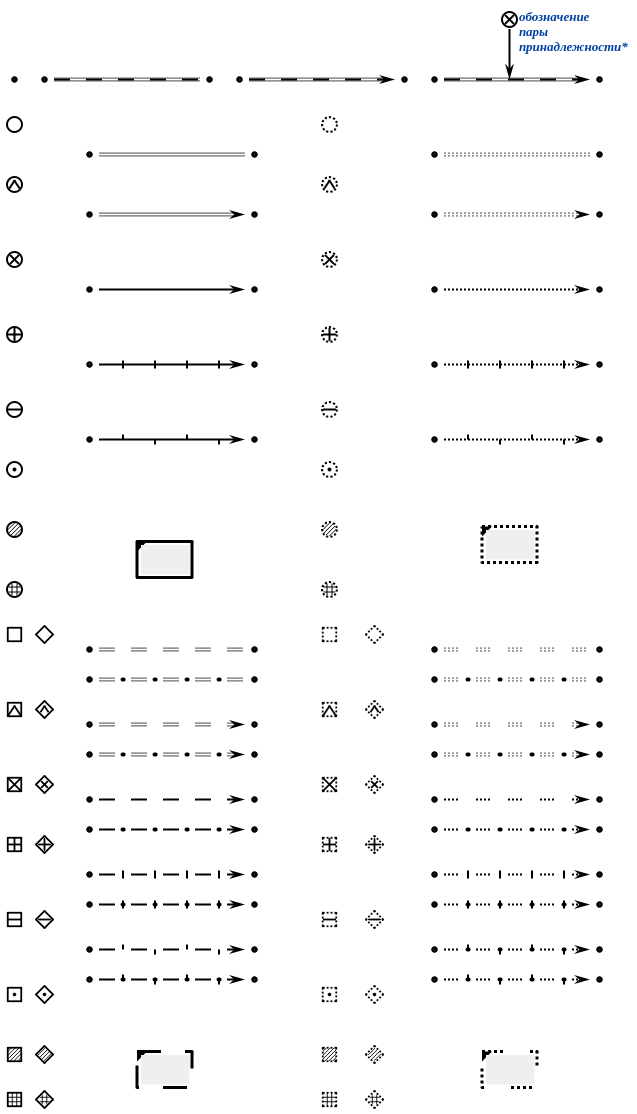
\includegraphics[scale=0.8]{images/intro/scg/SCg-full.png}
\end{figure}

\bigskip
Трудно сразу поверить, что на основе такого простого алфавита можно построить удобный и \uline{универсальный} \textit{графовый язык}. В рамках \textit{Документации Технологии OSTIS} мы постараемся Вас в этом убедить. Кроме того, нас не должна настораживать простота алфавита, поскольку человечество имеет большой опыт кодирования, хранения в памяти и передачи по каналам связи самых различных информационных ресурсов, используя алфавит, состоящий только из двух классов элементов --- единиц и нулей. 

Мы ведем речь о принципиально ином (графовом) способе кодирования информации в \textit{компьютерных системах}, но стараемся при этом свести это кодирование к достаточно простому алфавиту хотя бы для того, чтобы искусственно не усложнять проблему создания нового поколения компьютеров, основанных на указанном способе кодирования информации. 

Расширения \textit{Ядра SCg-кода} рассмотрим как направления перехода от текстов \textit{Ядра SCg-кода} к более компактным текстам. Но, поскольку это приводит к усложнению \textit{Синтаксиса SCg-кода} и, в первую очередь, к расширению \textit{Алфавита SCg-кода\scnsupergroupsign}, делать такие расширения необходимо обоснованно с учетом частоты встречаемости в рамках \textit{баз знаний ostis-систем} соответствующих фрагментов.

\subsection{Денотационная семантика SCg-кода}
\label{sec_scg_semantics}

В \textit{SCg-коде} выделяются Ядро SCg-кода и его расширения. 
\textbf{\textit{Алфавит Ядра SCg-кода\scnsupergroupsign}} --- алфавит \textit{sc.g-элементов}, графически изображаемых \textit{sc-элементы}. \textit{Алфавит Ядра SCg-кода\scnsupergroupsign} взаимно однозначно соответствует \textit{Алфавиту SC-кода\scnsupergroupsign}.

\textit{Денотационная семантика Ядра SCg-кода} соответствует \textit{Денотационной семантике SC-кода}. Это продемонстрировано на рисунке.

\textbf{\textit{Таблица. Алфавит Ядра SCg-кода\scnsupergroupsign}}
\begin{figure}[h]
	\centering
	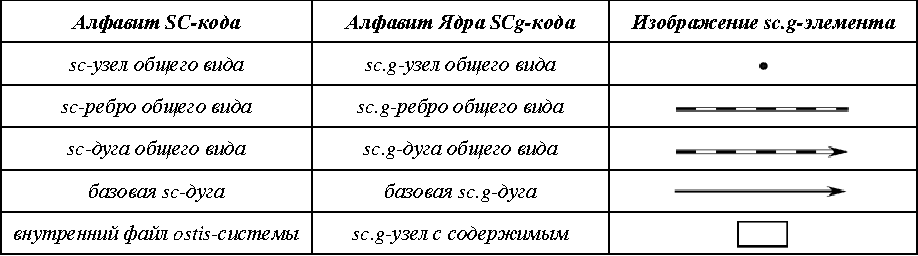
\includegraphics[scale=0.8]{images/intro/scg/SCg-core-alphabet.pdf}
\end{figure}

\textit{Алфавит Ядра SCg-кода\scnsupergroupsign} представлен следующими элементами:
\begin{textitemize}
	\item \textbf{\textit{sc.g-узел общего вида}} --- \textit{sc.g-элемент}, являющийся графическим изображением \textit{sc-узла общего вида}. Все \textit{sc-узлы}, не являющиеся знаками файлов, в тексте (конструкции) \textit{Ядра SCg-кода}, изображаются в виде небольших чёрных кругов одинакового диаметра, который обозначим через $\bm{d}$, и точная величина которого зависит от масштаба отображения \textit{sc.g-текста};
	
	\item \textbf{\textit{sc.g-ребро общего вида}} --- \textit{sc.g-элемент}, являющийся графическим изображением \textit{sc-ребра общего вида}. Каждое \textit{sc-ребро} в \textit{Ядре SCg-кода} изображается в виде широкой линии, в которой чередуются фрагменты со сплошной заливкой и без заливки, не имеющей самопересечений и имеющей общую толщину, равную примерно $\bm{0.7d}$;
	
	\item \textbf{\textit{sc.g-дуга общего вида}} --- \textit{sc.g-элемент}, являющийся графическим изображением \textit{sc-дуги общего вида}. Каждая \textit{sc-дуга} в \textit{Ядре SCg-кода} изображается в виде широкой линии, в которой чередуются фрагменты со сплошной заливкой и без заливки, не имеющей самопересечений, имеющей общую толщину, равную примерно $\bm{0.7d}$ и имеющей изображение стрелочки на одном из концов этой линии;
	
	\item \textbf{\textit{базовая sc.g-дуга}} --- \textit{sc.g-элемент}, являющийся графическим изображением \textit{базовой sc-дуги}. Каждая входящая в состав sc-текста \textit{базовая sc-дуга} в \textit{Ядре SCg--кода} изображается в виде линии произвольной формы, не имеющий самопересечений, имеющий толщину $\bm{0.4d}$, и имеющей изображение стрелочки на одном из ее концов;
	
	\item \textbf{\textit{внутренний файл ostis-системы}} --- \textit{sc-узел}, являющийся знаком \textit{внутреннего файла ostis-системы}, sc-знак \textit{внутреннего файла ostis-системы};
	
	\item \textbf{\textit{sc.g-узел с содержимым}} --- \textit{sc.g-узел}, имеющий содержимое, sc.g-узел, являющийся знаком внутреннего файла ostis-системы, sc.g-рамка. \textit{sc.g-рамка} --- это всегда прямоугольник, максимальный размер которого не ограничивается, но минимальный фиксируется и соответствует \textit{sc.g-рамке}, внутри которой обозначаемый ею \textit{файл} не отображается. Каждый входящий в sc-текст \textit{sc-узел, имеющий содержимое}, в \textit{Ядре SCg-кода} изображается в виде прямоугольника произвольного размера с толщиной линии $\bm{0.6d}$. Внутри этого прямоугольника отображается \textit{файл}, обозначаемый изображаемым \textit{sc-узлом}. Если нет необходимости изображать в тексте сам \textit{файл}, то \textit{sc-узел}, обозначающий такой \textit{файл}, в \textit{sc.g-тексте} изображается в виде прямоугольника со сторонами $\bm{2d}$ по вертикали и $\bm{4d}$ по горизонтали.
\end{textitemize}

\subsection{Иерархическое семейство подъязыков, семантически эквивалентных SCg-коду}
\label{sec_scg_extensions}

\begin{SCn}
\begin{scnrelfromlist}{ключевой знак}
	\scnitem{Первое направление расширения Ядра SCg-кода}
	\scnitem{Второе направление расширения Ядра SCg-кода}
	\scnitem{Третье направление расширения Ядра SCg-кода}
	\scnitem{Четвертое направление расширения Ядра SCg-кода}
	\scnitem{Пятое направление расширения Ядра SCg-кода}
	\scnitem{Шестое направление расширения Ядра SCg-кода}
	\scnitem{Седьмое направление расширения Ядра SCg-кода}
\end{scnrelfromlist}
\end{SCn}

\textbf{\textit{Первое направление расширения Ядра SCg-кода}}

\textit{Первое направление синтаксического расширения Ядра SCg-кода} --- это \uline{приписывание} некоторым \mbox{sc.g-элементам} \textit{основных sc-идентификаторов*} (чаще всего --- строковых идентификаторов, то есть имен) \textit{sc-элементов} , изображаемых этими \textit{sc.g-элементами}. Указываемые идентификаторы являются уникальным для каждого идентифицируемого (именуемого) \textit{sc.g-элемента}. Приписывание \textit{sc.g-элементам} уникальных идентификаторов дает возможность в рамках одного \textit{sc.g-текста} дублировать (копировать) некоторые \textit{sc.g-узлы} при условии, если \uline{всем} таким копиям будут приписаны соответствующие идентификаторы. Такое дублирование \textit{sc.g-узлов} является дополнительным средствам \uline{наглядного} размещения \textit{sc.g-текстов}. Кроме того, приписывание \textit{sc.g-элементу} соответствующего ему основного (уникального) \textit{sc-идентификатора*} представляет собой более компактный вариант изображения \textit{sc.g-текстов}.

\textbf{\textit{Пример sc.g-текста, трансформируемого по Первому направлению расширения Ядра SCg-кода}}

\begin{figure}[h]
	\centering
	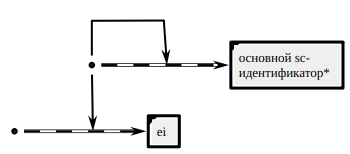
\includegraphics[scale=0.8]{images/intro/scg/scg_transf1.png}
\end{figure}

Здесь (в левом нижнем углу приведенного sc.g-текста) представлен \textit{sc.g-узел общего вида}, изображающий \textit{sc-узел общего вида}, которому соответствует \textit{основной sc-идентификатор*} в виде строки ``\textbf{\textit{ei}}''.

\bigskip
Трансформация \textit{sc.g-текста} по \textit{Первому направлению расширения Ядра SCg-кода}:
\begin{figure}[h]
	\centering
	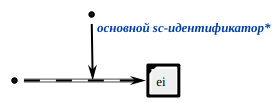
\includegraphics[scale=0.8]{images/intro/scg/scg_transf2.png}
\end{figure}
\textit{sc.g-узлу общего вида} изображающему \textit{sc-узел}, внешним идентификатором которого является строка ``\textit{основной sc-идентификатор*}'' и который, соответственно является знаком \textit{бинарного ориентированного отношения}, каждая \textit{пара} которого связывает идентифицируемый \textit{sc-элемент} с его основным внешним sc-идентификатором, приписывается указанный внешний идентификатор изображаемого им \textit{sc-элемента}.

\bigskip
Трансформация \textit{sc.g-текста} по \textit{Первому направлению расширения Ядра SCg-кода}:
\begin{figure}[h]
	\centering
	
\includegraphics[scale=0.8]{images/intro/scg/scg_transf3.png}
\end{figure}

В результате данной трансформации исходный \mbox{\textit{sc.g-текст}} трансформируется в один \textit{sc.g-общего вида}, которому приписывается \textit{основной sc-идентификатор} ``\textit{\textbf{ei}}''.

Подчеркнем, что рассматриваемая трансформация преобразует исходный текст Ядра \textit{SCg-кода} в текст, семантически эквивалентный, но принадлежащий не Ядру \textit{SCg-кода}, а его расширению.

\textbf{\textit{Второе направление расширения Ядра SCg-кода}}

\textit{Второе направление расширения Ядра SCg-кода} --- это уточнение типологии \textit{константных постоянных сущностей} и расширение \textit{Алфавита Ядра SCg-кода\scnsupergroupsign}, позволяющее типологию \textit{константных постоянных сущностей} привести в соответствие с синтаксической типологией новых вводимых элементов \textit{Алфавита SCg-кода\scnsupergroupsign}. Рассмотрим подробнее sc.g-элементы, знаки \textit{константных постоянных сущностей} различного вида. Графическим признаком \textit{константных постоянных sc-узлов} в конструкциях SCg-кода является их изображение в виде \uline{окружностей} диаметра $3d$, где $d$ --- диаметр sc.g-узла общего вида. Такое изображение является более компактной записью факта принадлежности заданного sc-узла (назовем его $\bm{vi}$) классу sc-констант и классу обозначений постоянных сущностей. Запись этого факта в \textit{Ядре SCg-кода} потребует (1) явного изображения sc-узла, обозначающего класс всевозможных константных sc-элементов (класс \textit{sc-констант}), (2) явного изображения базовой sc-дуги, соединяющего изображение sc-узла, обозначающего класс sc-констант, с изображением заданного константного sc-узла, (3) явного изображение sc-узла, обозначающего класс всевозможных sc-элементов, обозначающих \textit{постоянные сущности}, (4) явного изображения базовой sc-дуги, соединяющего изображение sc-узла, обозначающего класс обозначений \textit{постоянных сущностей} с изображением рассматриваемого sc-узла $\bm{vi}$ (см. \textit{Файл. Изображение спецификации sc.g-элемента средствами Ядра SCg-кода и Первого расширения Ядра SCg-кода}).

\textit{Второе направление расширения Ядра SCg-кода} --- это уточнение типологии \textit{константных постоянных сущностей} и расширение \textit{Алфавита Ядра SCg-кода\scnsupergroupsign}, позволяющее типологию \textit{константных постоянных сущностей} привести в соответствие с синтаксической типологией новых вводимых элементов \textit{Алфавита SCg-кода\scnsupergroupsign}. Рассмотрим подробнее sc.g-элементы, знаки \textit{константных постоянных сущностей} различного вида. Графическим признаком \textit{константных постоянных sc-узлов} в конструкциях SCg-кода является их изображение в виде \uline{окружностей} диаметра $3d$, где $d$ --- диаметр sc.g-узла общего вида. Такое изображение является более компактной записью факта принадлежности заданного sc-узла (назовем его $\bm{vi}$) классу sc-констант и классу обозначений постоянных сущностей. Запись этого факта в \textit{Ядре SCg-кода} потребует:
\begin{textitemize}
	\item явного изображения sc-узла, обозначающего класс всевозможных константных sc-элементов (класс \textit{sc-констант});  
	\item явного изображения базовой sc-дуги, соединяющего изображение sc-узла, обозначающего класс sc-констант, с изображением заданного константного sc-узла; 
	\item явного изображение sc-узла, обозначающего класс всевозможных sc-элементов, обозначающих \textit{постоянные сущности};
	\item явного изображения базовой sc-дуги, соединяющего изображение sc-узла, обозначающего класс обозначений \textit{постоянных сущностей} с изображением рассматриваемого sc-узла $\bm{vi}$ (см. \textit{Файл. Изображение спецификации sc.g-элемента средствами \textit{Ядра SCg-кода} и \textit{Первого расширения Ядра SCg-кода}}).
\end{textitemize}

\bigskip
Общепринятая запись данного факта выглядит следующим образом:

``\textit{sc-константа} $\ni \bm{vi}$; \textit{постоянная сущность} $\ni \bm{v_i};$''
\bigskip

\begin{textitemize}
	\item \textit{Константные постоянные sc-ребра} в конструкциях SCg-кода изображаются в виде двойной линии, каждая из которых имеет толщину примерно $d/7$, а расстояние между ними равно примерно $3d/7$. 
	\item \textit{Константные постоянные sc-дуги} изображаются в виде такой же двойной линии, но со стрелочкой. Все \textit{базовые sc-дуги}, а также все sc-узлы, имеющие содержимое, по определению являются \textit{константными постоянными sc-элементами}. 
	\item \textit{Константные sc.g-узлы}, изображаемые окружностями диаметра $3d$ и толщиной границы $d/5$, обозначают \textit{константные постоянные сущности}, о которых мало что известно, но известно то, что они не являются парами (то есть множествами, \textit{мощность*} которых равна 2) и, следовательно, не могут быть изображёны в виде sc.g-дуг или sc.g-рёбер. Но, если при этом об обозначаемой \textit{константной постоянной сущности} ($\bm{vi}$) известно, что она является классом сущностей, то явное указание принадлежности sc-элемента \textit{vi} всевозможных классов можно заменить на специальное графическое изображение sc-элемента \textit{vi}, предполагаемое указанную принадлежность. Это приводит к расширению  \textit{Алфавита SCg-кода\scnsupergroupsign} (см. \textit{Примеры sc.g-текстов, трансформируемых по Второму направлению расширения Ядра SCg-код}).
\end{textitemize}


Аналогичным образом (см. \textit{Примеры sc.g-текстов, трансформируемых по Второму направлению расширения Ядра SCg-код}) вводятся: 
\begin{textitemize}
	\item \textit{sc.g-узел}, являющийся изображением \textit{класса};  
	\item \textit{sc.g-узел}, являющийся изображением \textit{класса классов};  
	\item \textit{sc.g-узел}, являющийся изображением \textit{отношения}; 
	\item \textit{sc.g-узел}, являющийся изображением \textit{ролевого отношения}; 
	\item \textit{sc.g-узел}, являющийся изображением \textit{структуры};  
	\item \textit{sc.g-узел}, являющийся изображением \textit{небинарной связки};
	\item \textit{sc.g-узел}, являющийся изображением \textit{первичной сущности} (терминальной сущности, которая не является множеством, а также файлом, хранимым в памяти ostis-системы).
\end{textitemize}

Важное место среди константных постоянных сущностей занимают \textit{константные постоянные пары принадлежности}, обозначаемое соответствующими \textit{sc.g-дугами}. Такие пары принадлежности и обозначающие их sc.g-дуги бывают позитивными, негативными и нечеткими. Константная постоянная позитивная sc.g-дуга принадлежности есть ничто иное, как \textit{базовая sc.g-дуга}. Константная постоянная негативная sc.g-дуга принадлежности изображается в виде \textit{базовой sc.g-дуги}, перечеркнутой штриховыми черточками. Константная постоянная нечёткая sc.g-дуга принадлежности изображается в виде "недочеркнутой"{} \textit{базовой sc.g-дуги}, с каждой стороны которой отображаются штрихи, по длине равные половине от длины штрихов, которыми перечеркнута \textit{константная постоянная негативная sc.g-дуга}.

\textbf{\textit{Третье направление расширения Ядра SCg-кода}}

\textit{Третье направление расширения Ядра SCg-кода} --- это расширение его алфавита путем введения дополнительных sc.g-элементов, обозначающих \textit{константные временные сущности} различного вида. Признаком sc.g-элементов, обозначающих \textit{константные временные сущности} являются точечные линии (линии, состоящие из точек, размер которых равен размеру изображаемой линии и которые близко расположены друг к другу на расстоянии, равном половине их размера), с помощью которых рисуются окружности при изображении sc-узлов, а также линии при изображении sc-коннекторов.

Результатом \textit{Третьего направления расширения Ядра SCg-кода} является введение следующих видов \textit{sc.g-элементов} (см. \textit{Примеры sc.g-текстов, трансформируемых по Третьему направлению расширения Ядра SCg-кода}).

\textbf{\textit{Четвёртое направление расширения Ядра SCg-кода}}

\textit{Четвёртое направление расширения Ядра SCg-кода} --- это расширение его алфавита путем введения дополнительных элементов, обозначающих \textit{переменные постоянные сущности} различного вида. Признаком sc.g-элементов, обозначающих сущности указанного класса, являются квадратики для изображения обозначений \textit{переменных постоянных сущностей}, не являющихся бинарными связями, а также пунктирные и штрих-пунктирные линии для изображения \textit{переменных постоянных бинарных связей}. 

Подчеркнем, что \textit{переменные постоянные сущности} могут отличаться друг от друга по характеру их \textit{области значений*}. Этими значениями в общем случае могут быть как \textit{константные постоянные сущности}, так и \textit{переменные постоянные сущности}. В любом случае, значение \textit{переменной сущности} является либо \textit{константной сущностью}, либо \textit{переменной сущностью}. Если каждое значение переменной является константой, то такую переменную будем называть \textit{переменной первого уровня}. Если каждое значение переменной является \textit{переменной первого уровня}, то такую переменную будем называть \textit{переменной второго уровня}. 

\textbf{\textit{переменная постоянная сущность первого уровня}} (первичная sc-переменная), не являющаяся бинарной связью --- это переменная, каждым значением которой является \textit{константная постоянная сущность}, не являющаяся бинарной связью. Такая переменная изображается квадратиком, который ориентирован по вертикали и горизонтали. 

\textit{переменная постоянная сущность второго уровня} (вторичная sc-переменная), не являющаяся бинарной связью, изображается квадратиком, повернутым на 45$^\circ$. 

Указанная выше семантика таких изображений приписывается \uline{по умолчанию}. Это означает, что, если обозначаемая sc-переменная имеет более сложную структуру области её значений (является sc-переменной третьего и выше уровня или sc-переменной, значения которой имеют различный логический уровень), то эта область должна быть специфицирована явно, при этом такая sc-переменная в SCg-коде изображается так же, как первичная sc-переменная.

\textbf{\textit{Пятое направление расширения Ядра SCg-кода}}
	
\textit{Пятое направление расширения Ядра SCg-кода} --- это расширение его алфавита путем введения дополнительных \textit{sc.g-элементов}, обозначающих \textit{переменные временные сущности} различного вида. Указанные дополнительные \textit{sc.g-элементы} аналогичны тем, которые введены в рамках \textit{Четвертого направления расширения Ядра SCg-кода}, и отличаются только тем, что в \textit{Пятом направлении расширении Ядра SCg-кода} речь идёт о переменных \uline{временных} сущностях, а в \textit{Четвертом направлении расширения Ядра SCg-кода} --- о переменных \uline{постоянных} сущностях.

\textbf{\textit{Шестое направление расширения Ядра SCg-кода}}

\textit{Шестое направление расширения Ядра SCg-кода} --- это введение в SCg-код \textit{sc.g-контуров} и \textit{sc.g-шин} как средств структуризации sc.g-текстов и повышения наглядности при их размещении. Подчеркнем, что и sc.g-контуры, и sc.g-шины, и sc.g-рамки являются специальными видами sc.g-элементов. При этом sc.g-контуры и sc.g-рамки являются sc.g-ограничителями (ограничителями SCg-кода).

Каждый \textbf{\textit{sc.g-контур}} изображается (в 2D-модификации) в виде замкнутой ломаной линии со скругленными изломами, ограничивающей некоторый фрагмент sc.g-текста и обозначает множество всех \uline{sc-элементов}, sc.g-изображения которых оказались внутри этого контура. Толщина указанной линии составляет примерно $\bm{0.4d}$, где \textbf{\textit{d}} --- диаметр \textit{sc.g-узла общего вида}.

Обозначение \textit{множества sc-элементов}, изображаемое \textit{sc.g-контуром}, может быть как константным, так и переменным. Соответственно этому линия, изображающая \textit{sc.g-контур} может быть: 

\begin{textitemize}
	\item сплошной непунктирной линией,
	\item точечной непунктирной линией,
	\item сплошной пунктирной линией,
	\item точечной пунктирной линией.
\end{textitemize}

\bigskip
Семантическим эквивалентом \textit{sc.g-контуру} является \textit{sc.g-узел, обозначающий структуру}. Использование \textit{sc.g-контура} вместо указанного \textit{sc.g-узла} исключает необходимость явно изображать \textit{sc-дуги принадлежности}, выходящие из этого \textit{sc.g-узла}. Это существенно повышает уровень наглядности \textit{sc.g-текста}.

Если представленный внутри \textit{sc.g-контура} текст не является \textit{sc.g-текстом}, то считается, что на самом деле внутренностью \textit{sc.g-контура} является \textit{sc.g-текст}, являющийся результатом перевода предоставленного текста в \textit{SCg-код}.

Каждая \textbf{\textit{sc.g-шина}} представляет собой замкнутую или незамкнутую линию толщиной примерно равной диаметру \textit{sc.g-узла общего вида}, которая инцидентна только одному \textit{sc.g-элементу} и семантически ему эквивалентна. Идея введения \textit{sc.g-шин} заключается в увеличении «размеров» \textit{sc.g-элементов} для расширения их области инцидентности. Особенно актуально это для \textit{sc.g-узлов}, имеющих большое число инцидентных им \textit{sc.g-коннекторов}.

\bigskip
\textbf{\textit{Седьмое направление расширения Ядра SCg-кода}}
	
\textit{Седьмое направление синтаксического расширения Ядра SCg-кода} --- это переход от 2D-изображений \textit{sc.g-текстов} к 3D-изображениям.

Одним из вариантов трехмерного изображения \textit{sc.g-текстов} является следующий:
\begin{textitemize}
	\item все sc.g-узлы изображаются, как и ранее, \uline{плоскими} графическими примитивами. При изменении точки просмотра они \uline{всегда} "поворачиваются"{} параллельно плоскости экрана, но их масштаб (размер на экране) при удалении от точки просмотра \uline{уменьшается};
	\item аналогичным "плоским"\ образом изображаются \textit{sc.g-рамки} с их "внутренним"\ содержанием, а также внешние идентификаторы, приписываемые \textit{sc.g-элементам};
	\item \textit{sc.g-коннекторы} изображаются \uline{непересекающимися} линиями в трехмерном пространстве (заметим, что при изображении \textit{sc.g-текстов} на плоскости пересечение \textit{sc.g-коннекторов} часто снижает наглядность, "читабельность"{} \textit{sc.g-текстов}). Т.е. \textit{sc.g-коннекторы}, которые на плоскости изображаются двойными линиями, в пространстве  цилиндрическими, "трубчатыми линиями"{} с находящейся внутри тонкой, но просвечивающейся осевой линией;
	\item \textit{sc.g-контур} в пространстве визуализируется несколькими (!) специального вида точками --- например там, где есть точки инцидентности \textit{sc.g-контура} с \uline{внешними} \textit{sc.g-коннекторами}. При этом \textit{sc.g-контур} становится виден только по команде просмотра указываемого контура (указание контура --- это указание одной из его точек инцидентности). По этой команде цветом выделяются все граничные точки контура (точки инцидентности) и все внутренние \textit{sc.g-элементы} контура. Если просматривается  несколько контуров, то используется несколько цветов.
\end{textitemize}

Вторым вариантом 3D-визуализации \textit{sc.g-текстов} является размещение \textit{sc.g-текстов} на параллельных плоскостях (слоях) с “прошивками”\ между этими слоями, соединяющими синонимичные \textit{sc.g-узлы}, то есть \textit{sc.g-узлы}, имеющие одинаковые приписываемые им внешние идентификаторы. Такой вариант плоской, но многослойной визуализации \textit{sc.g-текстов} дает возможность широко использовать те средства просмотра и редактирования \textit{sc.g-текстов}, которые разработаны для плоской их визуализации.

\section{Язык внешнего линейного представления конструкций SC-кода --- SCs-код (Semantic Code string)}
\label{sec_scs}

\begin{SCn}
\begin{scnrelfromlist}{подраздел}
	\scnitem{\ref{sec_scs_syntax}~\nameref{sec_scs_syntax}}
	\scnitem{\ref{sec_scs_semantics}~\nameref{sec_scs_semantics}}
	\scnitem{\ref{sec_scs_extensions}~\nameref{sec_scs_extensions}}
\end{scnrelfromlist}

\begin{scnrelfromlist}{ключевое понятие}
	\scnitem{sc.s-предложение}
	\scnitem{sc.s-ограничитель}
	\scnitem{sc.s-разделитель}
	\scnitem{sc.s-модификатор}
	\scnitem{sc.s-элемент}
	\scnitem{sc.s-коннектор}
	\scnitem{sc.s-ребро}
	\scnitem{sc.s-дуга}
\end{scnrelfromlist}

\begin{scnrelfromlist}{ключевой знак}
	\scnitem{SCs-код}
	\scnitem{Алфавит SCs-кода\scnsupergroupsign}
	\scnitem{Синтаксис SCs-кода}
	\scnitem{Денотационная семантика SCs-кода}
	\scnitem{Иерархическое семейство подъязыков, семантически эквивалентных SCs-коду}
\end{scnrelfromlist}
\end{SCn}

\begin{SCn}
\scnheader{SCs-код}
\scnidtf{Semantic Code string}
\scnidtf{Язык линейного представления знаний ostis-систем}
\scnidtf{Множество всевозможных текстов \textit{SCs-кода}}
\scnidtf{Язык внешнего линейного представления конструкций внутреннего языка ostis-систем}
\end{SCn}

\textbf{\textit{SCs-код}} представляет собой множество линейных текстов (\textit{sc.s-текстов}), каждый из которых состоит из предложений (\textit{sc.s-предложений}), разделенных друг от друга двойной \textit{точкой с запятой} (разделителем \textit{sc.s-предложений}). При этом \mbox{\textit{sc.s-предложение}} представляет собой последовательность \textit{sc-идентификаторов}, являющихся именами описываемых \textit{сущностей} и разделяемых между собой различными \textit{sc.s-разделителями} и \textit{sc.s-ограничителями}.

\subsection{Синтаксис SCs-кода}
\label{sec_scs_syntax}

\begin{SCn}
	\scnheader{Алфавит SCs-кода\scnsupergroupsign}
	\scnidtf{Алфавит символов SCs-кода\scnsupergroupsign}
	\scnidtf{множество символов SCs-кода}
	\scnidtf{символ, используемый в текстах SCs-кода}
	\scnidtf{Язык внешнего линейного представления информационных конструкций
		внутреннего языка ostis-систем}
	\begin{scnreltoset}{объединение}
		\scnitem{Алфавит символов, используемых в sc.s-разделителях\scnsupergroupsign}
		\scnitem{Алфавит символов, используемых в sc.s-ограничителях\scnsupergroupsign}
		\scnitem{Алфавит символов, используемых в sc-идентификаторах\scnsupergroupsign}
			\begin{scnreltoset}{объединение}
				\scnitem{Алфавит символов, используемых в простых строковых sc-идентификаторах\scnsupergroupsign}
				\scnitem{Алфавит символов, используемых в sc-выражениях\scnsupergroupsign}			
			\end{scnreltoset}
		\scnitem{Алфавит символов, используемых в неоднозначных sc.s-изображениях sc-узлов\scnsupergroupsign}
	\end{scnreltoset}
\end{SCn} 

\textbf{\textit{Алфавит SCs-кода\scnsupergroupsign}} строится на основе современных общепринятых наборов символов, что позволяет упростить разработку средств для работы с \textit{sc.s-текстами} с использованием современных технологий.

В состав \textit{sc.s-текстов}, как и в состав текстов любых других языков, являющихся вариантами внешнего отображения текстов \textit{SC-кода}, могут входить различные файлы, в том числе естественно-языковые или даже файлы, содержащие другие \textit{sc.s-тексты}. В общем случае в таких файлах могут использоваться самые разные символы, в связи с чем будем считать, что в \textit{Алфавит SCs-кода\scnsupergroupsign} эти символы не включаются.

\textbf{Алфавит символов, используемых в \textit{sc.s-разделителях}\scnsupergroupsign} состоит из: пробел, точка с запятой, двоеточие, круглый маркер и знак равенства.

\textbf{Алфавит символов, используемых в \textit{sc.s-разделителях}\scnsupergroupsign}, изображающих связь инцидентности sc-элементов состоит из: `` < ''{}, `` > ''{}, `` | ''{}, `` - ''{}.



\textbf{Алфавит символов, используемых в \textit{sc.s-разделителях}} состоит из: пробел, точка с запятой, двоеточие, круглый маркер и знак равенства.

\textbf{Алфавит символов, используемых в \textit{sc.s-разделителях}}, изображающих связь инцидентности sc-элементов состоит из: `` < ''{}, `` > ''{}, `` | ''{}, `` --- ''{}.

\textbf{Базовый алфавит символов, используемых в \textit{sc.s-коннекторах}} состоит из: `` $\sim$ ''{}, знак подчеркивания, знак равенства, двоеточие, `` < ''{}, `` > ''{}, `` --- ''{}, `` | ''{}, `` / ''{}.
	
\textbf{Расширенный алфавит символов, используемых в \textit{sc.s-коннекторах}\scnsupergroupsign} состоит из:
	``$\in$''{}, 
	``$\ni$''{}, ``$\subseteq$''{}, ``$\supseteq$''{},   ``$\subset$''{}, ``$\supset$''{}, ``$\leq$''{},  ``$\geq$''{}, ``$\Leftarrow$''{}, ``$\Rightarrow$''{}, ``$\leftarrow$''{}, ``$\rightarrow$''{}, 
	``$\Leftrightarrow$''{}.


При необходимости комбинации указанных признаков перечисленные символы комбинируются так, как показано в параграфе "\textit{Описание sc.s-разделителей и sc.s-ограничителей}"{}.

Как в \textit{Базовом}, так и в \textit{Расширенном Алфавитах} \textit{sc.s-коннекторов} используются следующие общие признаки, характеризующие тип изображаемого \textit{sc-коннектора}:
\begin{textitemize}
	\item знак подчеркивания как признак изображений переменных \textit{sc-коннекторов} (один знак подчеркивания для \textit{sc-коннекторов}, являющихся первичными \textit{sc-переменными}, два знака подчеркивания для \textit{sc-коннекторов}, являющихся вторичными \textit{sc-переменными (sc-метапеременными)});
	\item вертикальная черта `` $ | $ ''{} как признак изображений \textit{негативных sc-дуг принадлежности}; 
	\item косая черта `` $ / $ ''{} как признак изображений \textit{нечетких sc-дуг принадлежности};
	\item тильда `` $ \sim $ ''{} как признак изображений \textit{временных sc-дуг принадлежности}.   
\end{textitemize}

Для упрощения процесса разработки исходных текстов \textit{баз знаний} с использованием \textit{SCs-кода} и создания соответствующих средств вводятся два алфавита символов. \textit{Базовый алфавит символов, используемых в sc.s-коннекторах\scnsupergroupsign} включает только символы, входящие в переносимый набор символов и имеющиеся на стандартной современной клавиатуре. Таким образом, для разработки исходных текстов баз знаний, использующих только \textit{Базовый алфавит символов, используемых в sc.s-коннекторах\scnsupergroupsign} достаточно обычного текстового редактора. \textit{Расширенный алфавит символов, используемых в sc.s-коннекторах\scnsupergroupsign} включает также дополнительные символы, которые позволяют сделать sc.s-тексты (и sc.n-тексты) более читабельными и наглядными. Для визуализации и разработки sc.s-текстов с использованием расширенного алфавита требуется наличие специализированных средств.

\textbf{Алфавит символов, используемых в \textit{sc.s-ограничителях}\scnsupergroupsign} состоит из: ``( ''{}, ``)''{}, ``*''{}.

\textbf{Алфавит символов, используемых в неоднозначных \textit{sc.s-изображениях sc-узлов}\scnsupergroupsign} состоит из:
``\{''{}, ``\}''{}, 
``-''{}, ``!''{}, ``~[ \,''{}, ``~] \,{}.

\bigskip
\textbf{\textit{Описание sc.s-разделителей и sc.s-ограничителей}}

\textbf{\textit{sc.s-разделитель}} и \textbf{\textit{sc.s-ограничитель}} являются важными элементами \textit{SCs-кода}.

Существует \textit{sc.s-разделитель}, используемый для структуризации \textit{sc.s-предложений} и \textit{sc.s-разделитель} \textit{sc.s-предложений}.

\textit{sc.s-разделить} --- разделитель, используемый в \textit{sc.s-текстах}. \textit{sc.s-разделитель} разбивается на:
\begin{textitemize}
	\item \textit{sc.s-разделитель}, используемый для структуризации \textit{\textit{sc.s-предложений}}.
	\begin{textitemize}
		\item Разделяет \textit{sc-идентификатор бинарного отношения} и второй компонент одной из связок этого отношения в случае, если указанное бинарное отношение и его связка связаны \textit{константной sc-дугой принадлежности}. Представляется в виде двоеточия.
		\item Разделяет \textit{sc-идентификатор бинарного отношения} и второй компонент одной из связок этого отношения в случае, если указанное бинарное отношение и его связка связаны \textit{переменной sc-дугой принадлежности}. Представляется в виде двойного двоеточия.
	\end{textitemize}
	\item \textit{sc.s-разделитель \textit{sc.s-предложений}}, представляется в виде двойной точки с запятой.    
\end{textitemize}

\bigskip
\textbf{\textit{sc.s-ограничитель}} представляется в виде: $(![  (\ast ]! \cup ![  \ast) ]!)$

Круглые скобки со звездочкой ограничивают присоединенные \textit{sc.s-предложения}, которые, в свою очередь, могут иметь в своем составе другие присоединенные \textit{sc.s-предложения}.

Также существует \textbf{\textit{sc.s-коннектор}}. Типология \textit{sc.s-коннекторов} полностью соответствует типологии \textit{sc.g-коннекторов}, и, тем более, \textit{sc-коннекторов}, т.к. она учитывает устоявшиеся традиции изображения связок целого ряда конкретных отношений.

\begin{SCn}
\scnheader{sc.s-коннектор}
\scnidtf{изображение \textit{sc-коннектора} во внешнем тексте SCs-кода или SCn-кода}
\scnsubset{sc.s-разделитель}
\end{SCn}

Выделяют следующие \textit{sc.s-коннекторы}:
\begin{textitemize}
	\item \textit{ориентированный \textit{sc.s-коннектор}},
	\item \textit{неориентированный \textit{sc.s-коннектор}};
	\item \textit{\textit{sc.s-коннектор}}, соответствующий \textit{sc.g-дуге принадлежности},
	\item \textit{\textit{sc.s-коннектор}}, соответствующий \textit{sc.g-коннектору}, который не является \textit{sc.g-дугой}.
\end{textitemize}

Типология \textit{sc.s-коннекторов} полностью соответствует типологии \textit{sc.g-коннекторов}, и, тем более, \textit{sc-коннекторов}, так как она учитывает устоявшиеся традиции изображения связок целого ряда конкретных отношений.

На множестве \textit{sc-элементов} задано бинарное ориентированное отношение инцидентности sc-элементов, а так же подмножество этого отношения --- отношение инцидентности входящих \textit{sc-дуг}, каждая пара которого связывает sc-дугу с тем sc-элементом, в который она входит. В \textit{SC-коде} \textit{sc-коннекторы} могут соединять между собой не только \textit{sc-узел} с \textit{sc-узлами}, но и \textit{sc-узел} с \textit{sc-коннектором} и даже \textit{sc-коннектор} с \textit{sc-коннектором}. В последнем случае, указывая инцидентность sc-коннекторов, необходимо уточнить, какой из них является соединяемым (связываемым), а какой-соединяющим (связующим). Поэтому отношение инцидентности, заданное на множестве sc-элементов является ориентированным. Первый компонент пары этого отношения – связующий \textit{sc-коннектор}, а второй --- связуемый \textit{sc-элемент}. Очевидно, что связующий \textit{sc-элемент} всегда является \textit{sc-коннектором}, а \textit{sc-узел} может быть только связуемым.

\textit{sc.s-разделитель}, изображающий связь инцидентности \textit{sc-элементов} разбивается на:
\begin{textitemize}
	\item знак инцидентности “правого” \textit{sc-коннектора} --- знак инцидентности \textit{sc-коннектора}, \textit{sc-идентификатор} которого находится справа, изображается в виде `` $ \vdash$ ''{};
	\item знак инцидентности “левого” \textit{sc-коннектора} --- знак инцидентности \textit{sc-коннектора}, \textit{sc-идентификатор} которого находится слева, изображается в виде `` $ \dashv$ ''{};
	\item знак инцидентности входящей \textit{sc-дуги} справа --- знак инцидентности \textit{sc-дуги}, \textit{sc-идентификатор} который находится справа, изображается в виде `` $ |<$ ''{};
	\item знак инцидентности входящей \textit{sc-дуги} слева --- знак инцидентности \textit{sc-дуги}, \textit{sc-идентификатор} который находится слева, изображается в виде `` $ >| $ ''{}.
\end{textitemize}

\begin{SCn}
\scnheader{sc.s-разделитель, изображающий связь инцидентности sc-элементов}
\begin{scnrelfromset}{разбиение}
	\scnitem{знак инцидентности “правого” sc-коннектора}
	\begin{scnindent}
		\scnidtf{знак инцидентности sc-коннектора, sc-идентификатор которого находится справа}
		\scneqfileclass{|-}
	\end{scnindent}
	\scnitem{знак инцидентности “левого” sc-коннектора}
	\begin{scnindent}
		\scnidtf{знак инцидентности sc-коннектора, sc-идентификатор которого находится слева}
		\scneqfileclass{-|}
	\end{scnindent}
	\scnitem{знак инцидентности входящей sc-дуги справа}
	\begin{scnindent}
		\scnidtf{знак инцидентности sc-дуги, sc-идентификатор который находится справа}
		\scneqfileclass{|<}
	\end{scnindent}
	\scnitem{знак инцидентности входящей sc-дуги слева}
	\begin{scnindent}
		\scnidtf{знак инцидентности sc-дуги, sc-идентификатор который находится слева}
		\scneqfileclass{>|}
	\end{scnindent}
\end{scnrelfromset}
\end{SCn}

Указанные \textit{sc.s-разделители} с точки зрения синтаксической структуры \textit{sc.s-предложений} аналогичны \textit{sc.s-коннекторам}, но с точки зрения их денотационной семантики в отличие от \textit{sc.s-коннекторов} они не являются изображениями соответствующих sc-коннекторов
\newpage
\textbf{\textit{Описание изображения sc.s-коннекторов в Базовом и Расширенном алфавите SCg-кода\scnsupergroupsign}}

\begin{figure}[h]
	\centering
	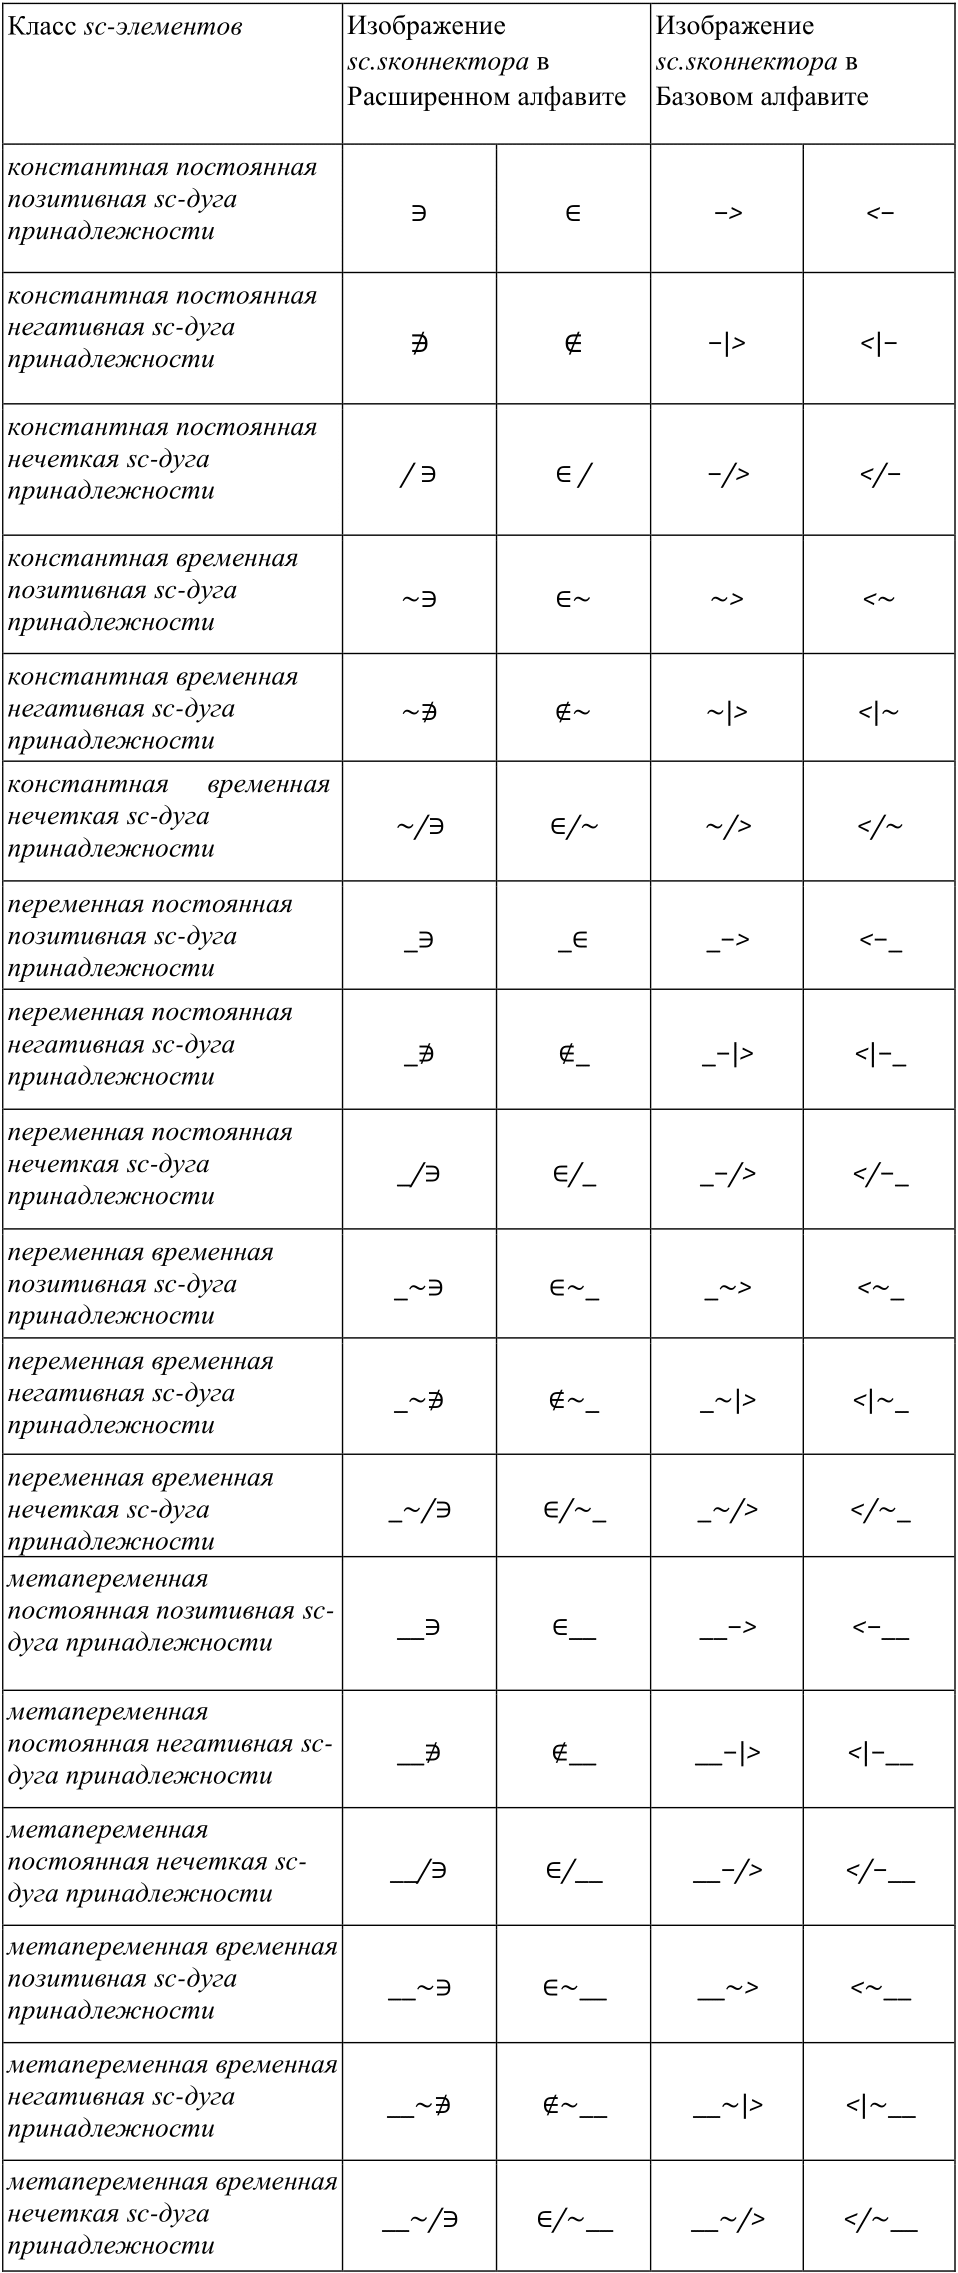
\includegraphics[scale=0.3]{images/intro/scs_membership_connectors_0.png}
\end{figure}

Знак равенства является \textit{sc.s-разделителем} двух \textit{sc-идентификаторов}, которые идентифицируют (именуют) одну и ту же сущность и, соответственно, являются \textit{sc-идентификаторами*} (внешними уникальными изображениями) одного и того же \textit{sc-элемента}. При этом из указанных двух sc-идентификаторов чаще всего один является простым \textit{sc-идентификатором}, а второй --- \textit{sc-выражением}. Реже оба эти \textit{sc-идентификатора} являются \textit{sc-выражениями}. И совсем редко оба они являются простыми sc-идентификаторами. Последнее обозначает то, что оба эти \textit{sc-идентификатора} являются основными \textit{sc-идентификаторами*} одного и того же \textit{sc-элемента}. Пример:
\textit{SC-код} = sc.s-текст;;

Здесь первый \textit{sc-идентификатор} является \textit{именем собственным}, а второй --- \textit{именем нарицательным}.

При трансляции \textit{sc.s-текста} в \textit{SC-код} знаку равенства на некотором этапе может быть поставлено в соответствие \textit{sc-ребро}, принадлежащее отношению \textit{синонимии}* \textit{sc-элементов}, идентифицируемых \mbox{\textit{sc-идентификаторами}}, связанными знаком равенства. Но на последующем этапе указанное \textit{sc-ребро} \uline{удаляется}, а связанные им \textit{sc-элементы} \uline{склеиваются}. Таким образом \textit{sc-ребро}, принадлежащее отношению \textit{синонимии}* sc-элементов, имеет не только денотационную, но и операционную семантику.

Знак равенства с включением --- изображение \textit{sc-дуги}, принадлежащей отношению погружения*, связывающей два \textit{sc-узла}, обозначающих \textit{sc-тексты}, первый из которых является погружающим, а второй (в который указанная \textit{sc-дуга} входит) является погружаемым, вводимым в состав первого \textit{sc-текста}. 

\textit{sc-дуга}, принадлежащая отношению погружения*, интерпретируется как команда погружения одного sc-текста в состав другого. При выполнении этой команды (1) все sc-элементы погружаемого \textit{sc-текста} становятся элементами, принадлежащими погружающему sc-тексту, (2) все синонимичные \textit{sc-элементы}, оказавшиеся в составе погружающего \textit{sc-текста}, склеиваются, (3) \textit{sc-узел}, обозначающий погружаемый \textit{sc-текст}, а так же спецификация этого \textit{sc-текста} (включая перечень всех его \textit{sc-элементов}) погружается в историю эволюции базы знаний вместе со спецификацией события погружения рассматриваемого \textit{sc-текста} в состав базы знаний.

Указанные \textit{sc.s-коннекторы} отличаются от остальных \textit{sc.s-коннекторов} тем, что они и соответствующие им sc-коннекторы (sc-ребра, принадлежащих отношению синонимии sc-элементов и sc-дуги, принадлежащие отношению погружения одного sc-текста в состав другого) имеют не только денотационную, но и операционную семантику, так как являются командами склеивания и командами погружения.

\bigskip
\textbf{\textit{Описание sc.s-предложений}}

\begin{SCn}
\scnheader{sc.s-предложение}
\scnidtf{минимальный семантически целостный фрагмент sc.s-текста}
\scnidtf{минимальный sc.s-текст}
\end{SCn}

\textit{sc.s-предложение}, (1) \uline{состоящее} или из двух \textit{sc-идентификаторов}, соединенных между собой \textit{\mbox{sc.s-коннектором}}, или из трех \textit{sc-идентификаторов}, разделенных \textit{sc.s-разделителями, изображающими связь инцидентности sc-элементов}, и (2) завершающееся \textit{двойной точкой с запятой}.

Нетрудно заметить, что простые sc.s-предложения по сути аналогичны триплетам языка RDF (\mbox{RDF-триплетам}), за тем исключением, что \textit{простое sc.s-предложение} можно "развернуть"{} при помощи \textit{Операции конверсии sc.s-предложений*} не меняя при этом его смысл, а RDF-триплет нельзя. Это является одной из причин, по которой, в отличие от RDF-триплетов, в простых \mbox{sc.s-предложениях} \textit{\mbox{sc.s-коннекторы}} и \textit{\mbox{sc.s-разделители}, изображающие связь инцидентности \mbox{sc-элементов}} не могут быть опущены, поскольку они в том числе показывают направление изображаемой ими связи между sc-элементами.

Признаком завершения любого \textit{sc.s-предложения}, то есть последними его символами является \textit{двойная точка с запятой}, которую, следовательно, можно считать разделителем \textit{sc.s-предложений}.

Выделяют следующие операции над sc.s-предложениями:
\begin{textitemize}
	\item \textbf{Операция конверсии sc.s-предложения*}
	
		Каждое \textit{sc.s-предложение} (в том числе, и \textit{простое sc.s-предложение}) можно преобразовать в семантически эквивалентное ему \textit{sc.s-предложение} путем конверсии ("разворота"{}) цепочки компонентов \textit{sc.s-предложения}. Так, например, при конверсии ("развороте") простого \textit{\mbox{sc.s-предложения}} (1) первый его \textit{\mbox{sc-идентификатор}} (первый компонент этого \textit{\mbox{sc.s-предложения}}) становится третьим компонентом конвертированного \textit{ \mbox{sc.s-предложения}}, (2) второй его \textit{\mbox{sc-идентификатор}} (третий компонент исходного \textit{\mbox{sc.s-предложения}}) становится первым компонентом "конвертированного"\ \textit{\mbox{sc.s-предложения}} и (3) второй компонент исходного \textit{\mbox{sc.s-предложения}} (\textit{\mbox{sc.s-коннектор}} или \textit{\mbox{sc.s-разделитель}, изображающий связь инцидентности \mbox{sc-элементов}}, соединяющий указанные выше компоненты) остается вторым компонентом конвертированного \textit{\mbox{sc.s-предложения}}, но меняет направленность ("$\ni$"\ заменяется на "$\in$"\ и наоборот, "$\supset$"\ на "$\subset$"\ и наоборот, "$\Rightarrow$"\ на "$\Leftarrow$"\ и наоборот и так далее).
	
	\item \textbf{Операция присоединения sc.s-предложения*}
		
		Операция соединения двух \textit{sc.s-предложений} при совпадении последнего компонента первого предложения с первым компонентом второго.
		В результате выполнения данной операции:
		\begin{textitemize}
			\item первый компонент второго \textit{sc.s-предложения} удаляется;
			\item оставшаяся часть второго предложения окружается \textit{sc.s-ограничителем} присоединенных предложений ("(*"{} и "*)"{}). Разделитель \textit{sc.s-предложений} (";;"{}) также попадает внутрь указанного ограничителя;
			\item полученная конструкция помещается между последним компонентом первого предложения и разделителем \textit{sc.s-предложений}, которым заканчивалось первое предложение;
			\item второе предложение, таким образом, становится \textit{присоединенным sc.s-предложением}.
		\end{textitemize}
	
		Аналогичным образом к любому присоединенному \textit{sc.s-предложению} могут "пристыковываться"\ другие присоединенные \textit{sc.s-предложения}, в общем случае уровень такой вложенности не ограничен.
		
		Присоединенные \textit{sc.s-предложения} используются для того, чтобы продолжить спецификацию какого-либо sc-элемента, \textit{sc-идентификатор} которого является последним компонентом в рамках какого-либо sc.s-предложения, не начиная при этом нового \textit{sc.s-предложения} и, таким образом, не дублируя указанный \mbox{sc-идентификатор}. Внутрь присоединенных sc.s-предложений также могут встраиваться другие присоединенные \textit{sc.s-предложения}, в общем случае уровень вложенности таких предложений не ограничен. Таким образом присоединенные \textit{sc.s-предложения} описывают "ветвление"{} \textit{sc.s-предложений}, при этом точками такого "ветвления"{} выступают \textit{sc-идентификаторы}, входящие в состав этих \textit{sc.s-предложений}.
		
		Благодаря введению \textit{присоединенных sc.s-предложений} появляется возможность любой \textit{sc-текст} изобразить в виде одного \textit{sc.s-предложения}, содержащего необходимое количество \textit{присоединенных sc.s-предложений}. Таким образом, \textit{SCs-код} по выразительной мощности становится эквивалентным \textit{SCn-коду}.
	
	\item \textbf{Операция слияния sc.s-предложений*}
		
		Операция присоединения \textit{простого sc.s-предложения} к \textit{sc.s-предложению}, у которого последний sc.s-коннектор совпадает с \textit{sc.s-коннектором} \textit{простого sc.s-предложения}, а предшествующий указанному \textit{sc.s-коннектору} sc-идентификатор совпадает с первым sc-идентификатором простого sc.s-предложения.
		
		В результате выполнения этой операции совпадающие sc-идентификаторы и sc.s-коннекторы соединяемых sc.s-предложений "склеиваются"{} , а последние sc-идентификаторы соединяемых \textit{sc.s-предложений} становятся последними компонентами объединенного \textit{sc.s-предложения},
		разделенными \textit{точкой с запятой}. Аналогичным образом можно присоединять сколько угодно простых \textit{sc.s-предложений}.
	
	\item \textbf{Операция разложения sc.s-предложений на простые sc.s-предложения*}
		
		Каждое \textit{sc.s-предложение} можно разложить на множество \textit{простых sc.s-предложений}, т.е. представить в виде последовательности \textit{простых sc.s-предложений}.
	
	\item \textbf{Операция разложения sc.s-предложений на простые sc.s-предложения с sc.s-разделителем, изображающим связь инцидентности sc-элементов*}
		
		Каждое \textit{sc.s-предложение} (в том числе и \textit{простое sc.s-предложение} с \textit{sc.s-коннектором}) можно представить в виде семантически эквивалентной последовательности \textit{простых \mbox{sc.s-предложений}} с \textit{sc.s-разделителем, изображающим связь инцидентности \mbox{sc-элементов}}.
		
		Данная операция осуществляет \uline{однозначное} (!) формирование множества \textit{простых \mbox{sc.s-предложений}} указанного вида.
\end{textitemize}

Операции, заданные на множестве \textit{sc.s-предложений} можно разделить на три группы:
\begin{textitemize}
	\item группа операций конверсии \textit{sc.s-предложений}, состоящая из одной операции;
	\item группа операций соединения \textit{sc.s-предложений};
	\item группа операций декомпозиции \textit{sc.s-предложений} и, в частности, операций разложения \textit{sc.s-предложений}.
\end{textitemize}

\bigskip
\textbf{\textit{компонент sc.s-предложения*}}

Каждое \textit{sc.s-предложение} представляет собой последовательность (1) \textit{sc-идентификаторов}, \mbox{(2) \textit{sc.s-коннекторов}} или \textit{sc.s-разделителей}, изображающих связь инцидентности \textit{sc-элементов}, (3) \textit{точек с запятыми}, (4) \textit{ограничителей присоединенных sc.s-предложений}, завершаемая \textit{двойной точкой с запятой}. При этом непосредственно соседствовать друг с другом не могут ни \textit{\mbox{sc-идентификаторы}}, ни \textit{\mbox{sc.s-коннекторы}}, ни, очевидно, \textit{точки с запятыми} и \textit{ограничители присоединенных sc.s-предложений}.\\
Между \textit{sc-идентификаторами} в рамках \textit{sc.s-предложения} может находиться либо \textit{точка с запятой}, либо \textit{sc.s-коннектор}, либо \textit{sc.s-разделитель}, изображающий связь инцидентности \textit{sc-элементов}. Слева и справа от \textit{sc.s-коннектора} и от \textit{sc.s-разделителя}, изображающего связь инцидентности \textit{sc-элементов}, должны находиться \textit{sc-идентификаторы}.

Указанные \textit{sc-идентификаторы}, \textit{sc.s-коннекторы} и \textit{sc.s-разделители}, изображающие связь инцидентности \textit{sc-элементов}, считаются компонентами соответствующего \textit{sc.s-предложения}. Понятие "быть компонентом sc.s-предложения"{} является относительным понятием (отношением), т.к. в состав некоторых компонентов \textit{sc.s-предложения} (в состав \textit{sc-идентификаторов}, являющихся \textit{sc.s-выражениями}, ограничиваемыми фигурными или квадратными скобками) могут входить других \textit{sc.s-предложения}, состоящие из своих компонентов.

\bigskip
\textbf{\textit{sc.s-модификатор*}}

Это дополнительный вид компонентов \textit{sc.s-предложений}. Каждый \textit{sc.s-модификатор}, являющийся компонентом некоторого \textit{sc.s-предложения}, представляет собой \textit{sc-идентификатор}, обозначающий множество (чаще всего, отношение), которому принадлежит sc-коннектор, изображенный \textit{sc.s-коннектором}, который предшествует указанному \textit{sc-идентификатору}. Признаком \textit{sc.s-модификатора} является \textit{двоеточие} (или \textit{двойное двоеточие}), которое ставится после \textit{sc.s-модификатора} и отделяет его либо от следующего за ним другого \textit{sc.s-модификатора} для этого же \textit{sc.s-коннектора}, либо от следующего за ним \textit{sc-идентификатора}, соответствующего sc-элементу, который инцидентен sc-коннектору, изображенному \textit{sc.s-коннектором}, находящимся левее рассматриваемого \textit{sc-идентификатора} после одного или нескольких \textit{sc.s-модификаторов}. Обычное ("одинарное"{}) \textit{двоеточие} обозначает, что sc-элемент, изображенный соответствующим \mbox{sc.s-модификатором}, связан с sc-коннектором, изображенным левее этого \mbox{sc.s-модификатора}, \textit{базовой \mbox{sc-дугой}} (\textit{константной постоянной позитивной \mbox{sc-дугой} принадлежности}), \textit{двойное двоеточие} обозначает, что указанные элементы связаны \textit{переменной постоянной позитивной \mbox{sc-дугой} принадлежности}.

\begin{SCn}
\scnheader{sc.s-текст}
\scnidtf{конкатенация \textit{sc.s-предложений}}
\scnidtf{последовательность \textit{sc.s-предложений}, разделяемых \textit{двойными точками с запятой}}
\end{SCn}

\textbf{\textit{sc.s-предложение}} является минимальным \textit{sc.s-текстом}. Смысл sc.s-текста (а также \textit{sc.s-текста, включенного в структуру} не зависит от порядка \textit{\mbox{sc.s-предложений}} в этих sc-текстах. Т.е. перестановка \textit{\mbox{sc.s-предложений}} в рамках таких \mbox{sc.s-текстов} смысла этих \mbox{sc.s-текстов} не меняет (т.е. приводит к семантически эквивалентным \mbox{sc.s-текстам}), но сильно влияет на трудоемкость человеческого восприятия (на "читабельность"{}) этих текстов.

\newpage
\subsection{Денотационная семантика SCs-кода}
\label{sec_scs_semantics}

\textbf{\textit{Таблица. Алфавит sc.s-коннекторов, соответствующих sc.g-дугам принадлежности\scnsupergroupsign}}
\begin{figure}[h]
	\centering
	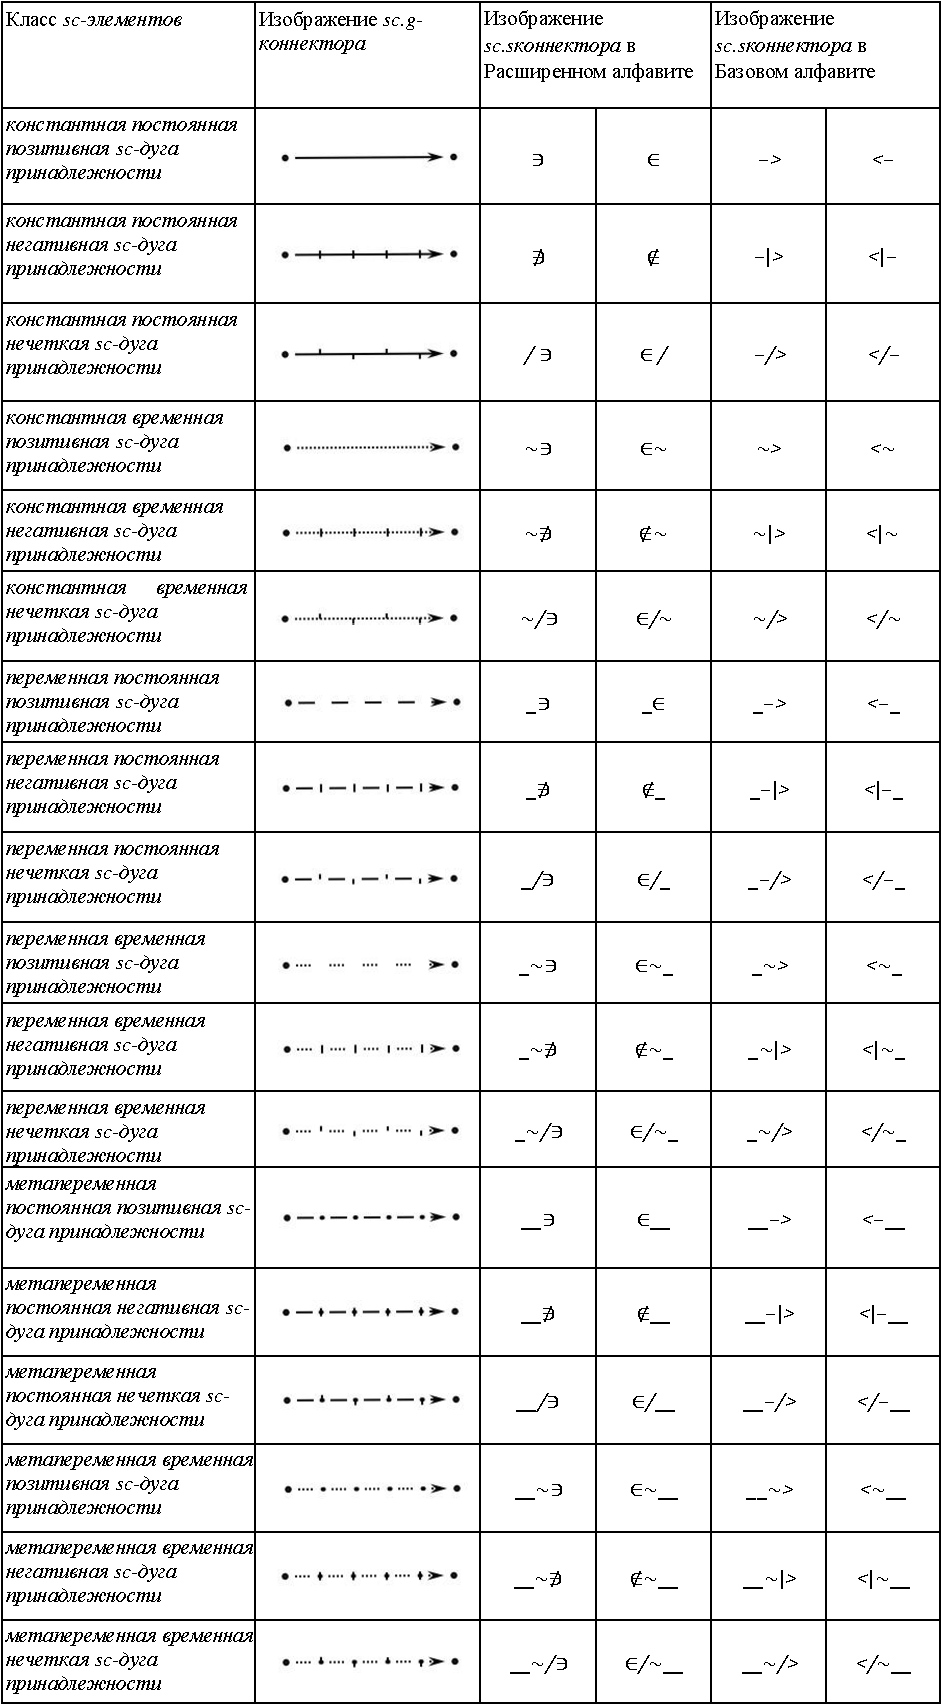
\includegraphics[scale=0.8]{images/intro/scs_membership_connectors.pdf}
\end{figure}

%---------------------------------------------

\textbf{\textit{Таблица. Алфавит sc.s-коннекторов, соответствующих sc.g-коннекторам, которые не являются sc.g-дугами принадлежности\scnsupergroupsign}}


\begin{figure}[h]
	\centering
	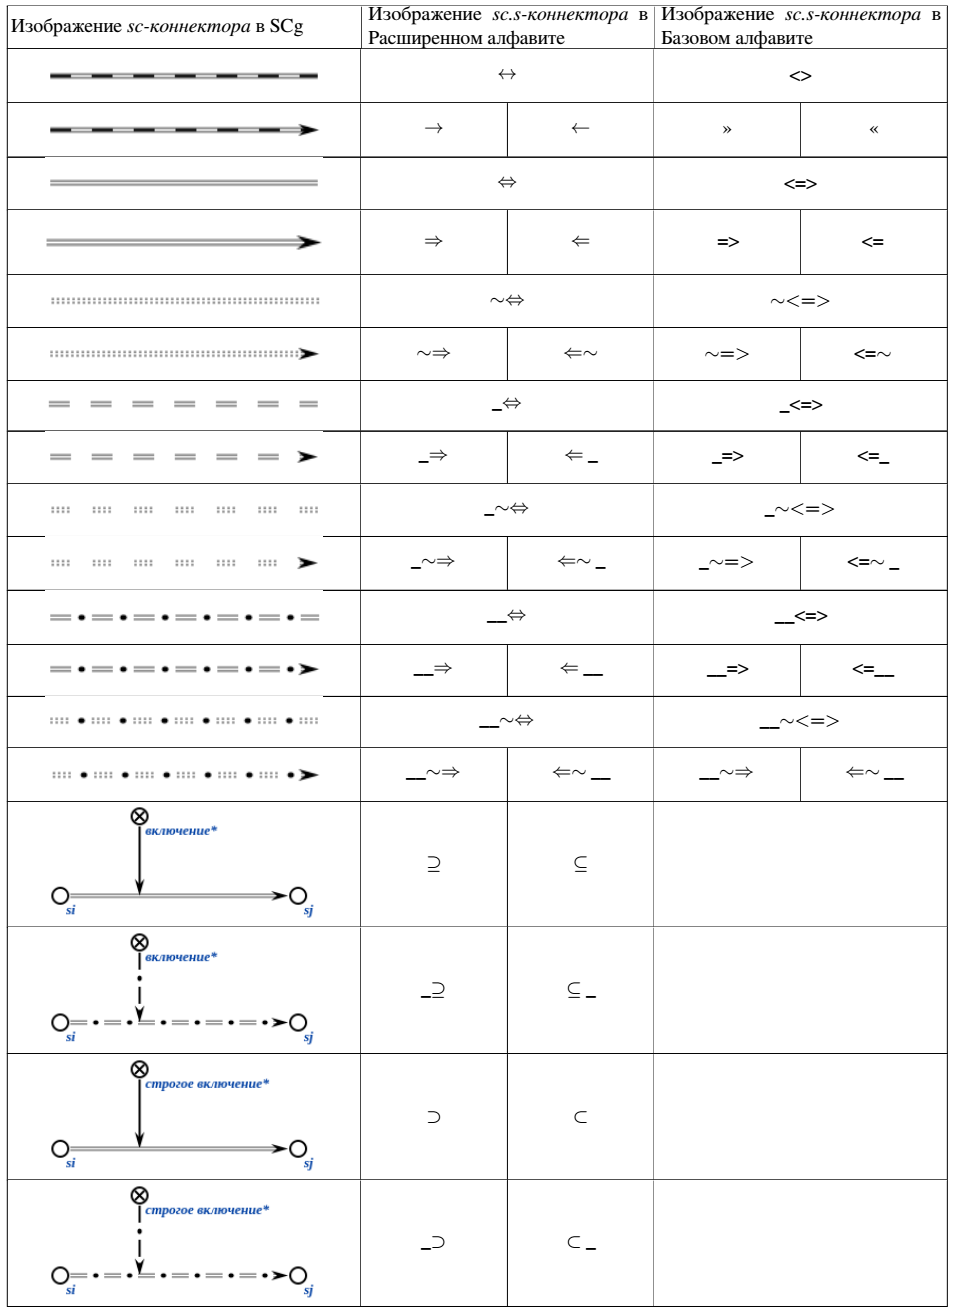
\includegraphics[scale=0.5]{images/intro/scs_non_membership_connectors_1.png}
\end{figure}

\begin{figure}[h]
	\centering
	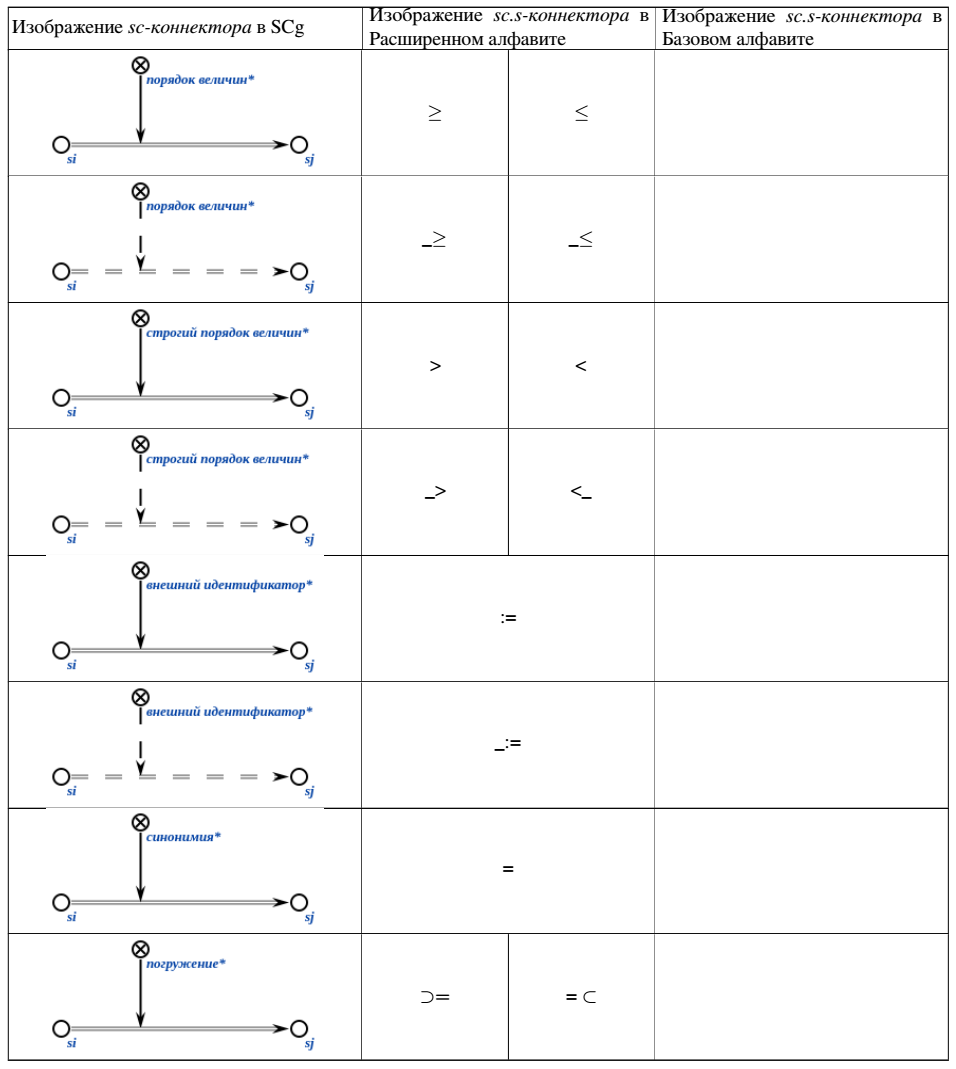
\includegraphics[scale=0.5]{images/intro/scs_non_membership_connectors_2.png}
\end{figure}

\newpage
\textbf{\textit{Примеры синтаксической трансформации sc.s-предложений с использованием Расширенного алфавита sc.s-коннекторов и соответствующие семантически эквивалентные конструкции в SCg-коде}}

\begin{SCn}
\scnfilelong{\textbf{\textit{si}}~$\Rightarrow$~\textit{включение*}:~\textbf{\textit{sj}}}
\scnrelfrom{синтаксическая трансформация}{
	\scnfilelong{\textbf{\textit{si}}~$\supseteq$~\textbf{\textit{sj}}}}
\begin{scnindent}
	\scnrelboth{семантическая эквивалентность}{
		\begin{figure}[h]
			\centering
			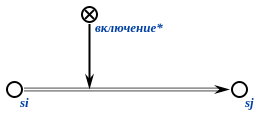
\includegraphics[scale=0.8]{images/intro/scs/sc.s-connectors/examples/scs_transf_inclusion_const.png}
	\end{figure}}
\end{scnindent}
\end{SCn}

\newpage

\begin{figure}[h]
	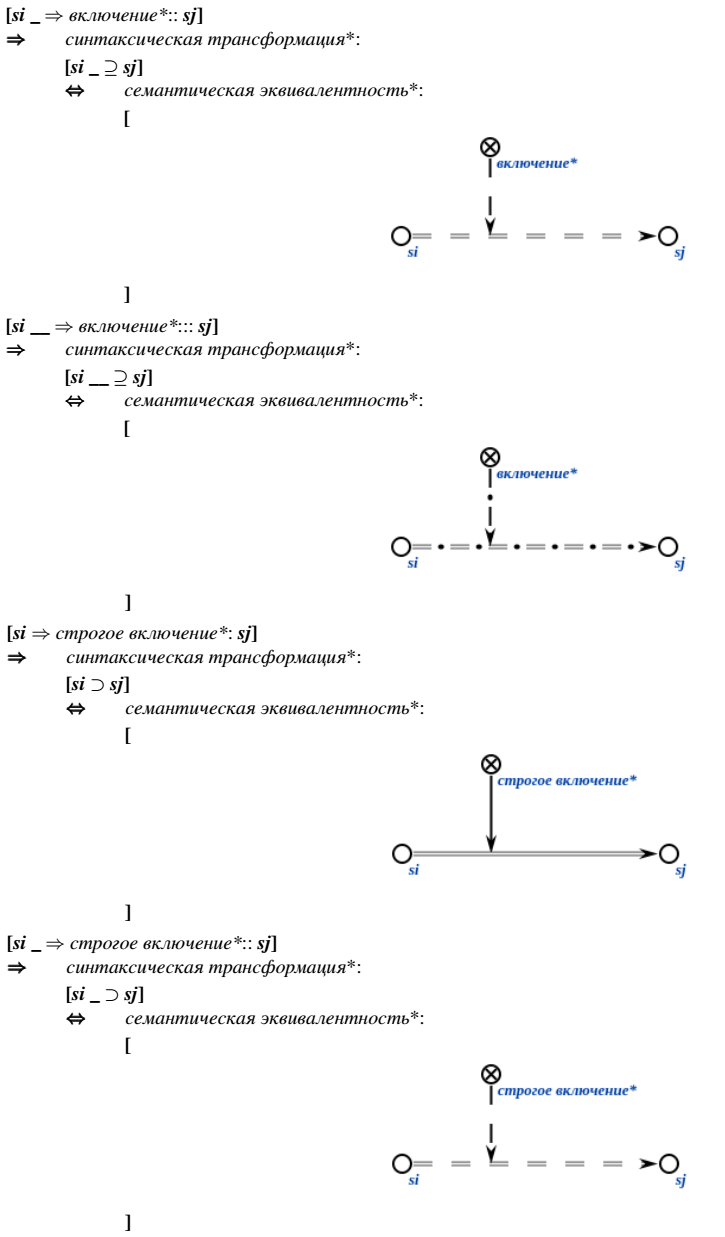
\includegraphics[scale=0.5]{images/intro/scs/sc.s-connectors/examples/example_1.png}
\end{figure}

\newpage
\begin{figure}[h]
	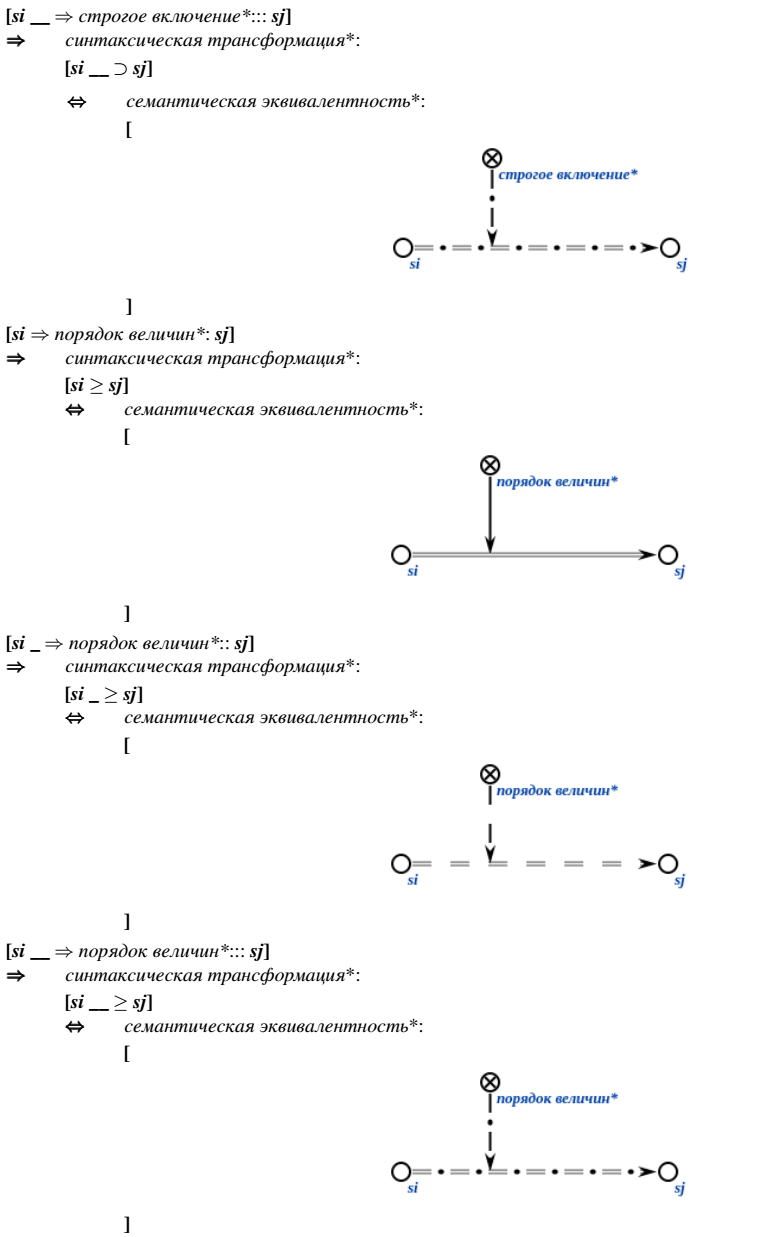
\includegraphics[scale=0.5]{images/intro/scs/sc.s-connectors/examples/example_2.png}
\end{figure}

\newpage
\begin{figure}[h]
	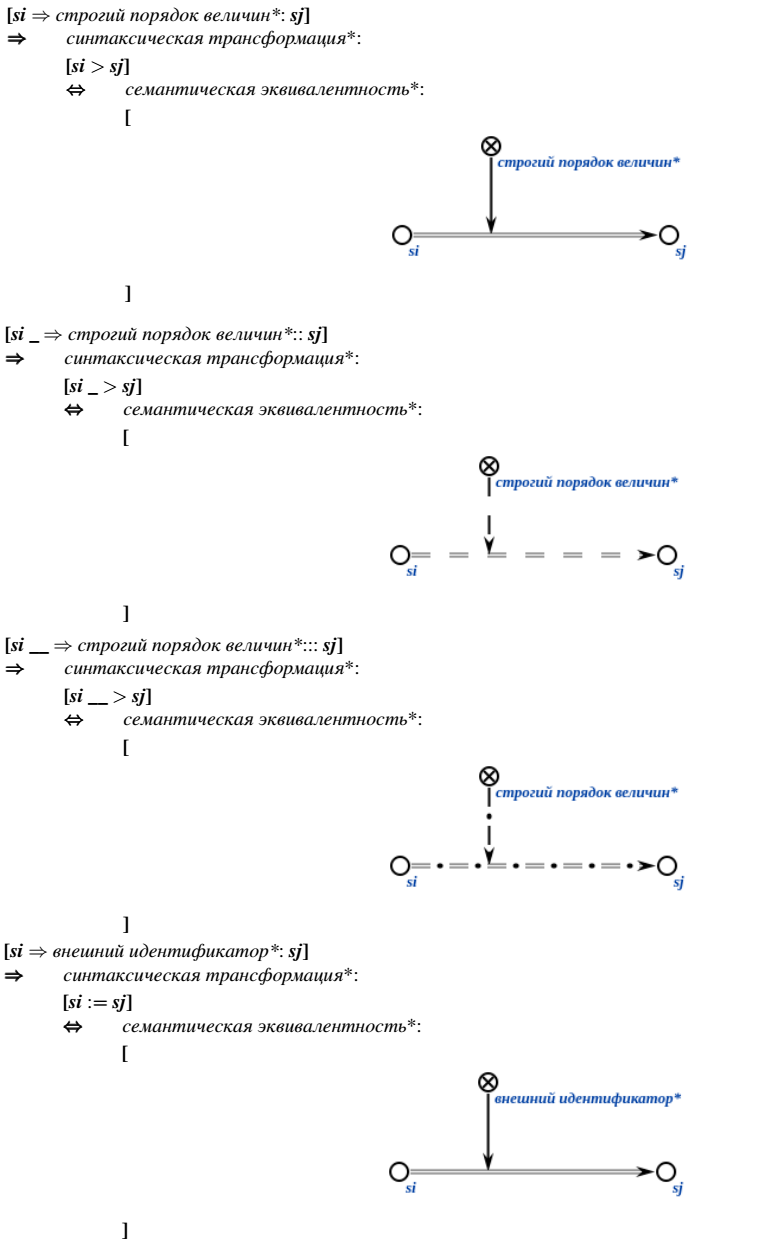
\includegraphics[scale=0.5]{images/intro/scs/sc.s-connectors/examples/example_3.png}
\end{figure}

\newpage
\begin{figure}[h]
	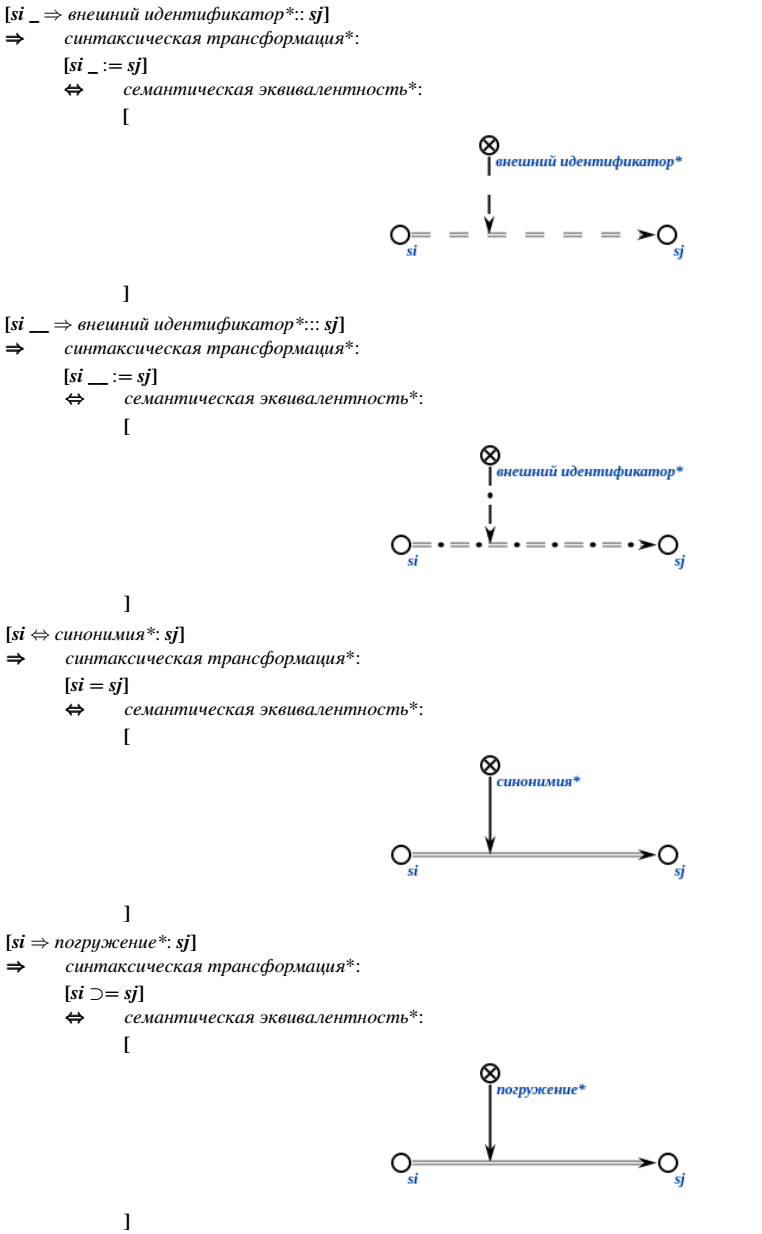
\includegraphics[scale=0.5]{images/intro/scs/sc.s-connectors/examples/example_4.png}
\end{figure}

Аналогичным образом может быть описана трансформация предложений, содержащих любые классы \textit{sc.s-коннекторов}, за исключением тех классов \textit{sc.s-коннекторов}, которые соответствуют классам \textit{sc-коннекторов}, входящим в \textit{Ядро SC-кода}.

В общем случае \textit{sc-элементы}, инцидентные \textit{sc-коннекторам}, классы которых описаны в данном примере, могут быть как \textit{sc-константами}, так и \textit{sc-переменными} (в том числе \textit{sc-метапеременными}). При этом как \textit{переменному sc-коннектору} может соответствовать \textit{константный sc-узел}, так и \textit{константному sc-коннектору} может соответствовать \textit{переменный sc-узел} (например, если возникает необходимость переменному sc-узлу приписать \textit{внешний идентификатор*}). Последняя ситуация встречается не очень часто и возникает в случае, когда область определения соответствующего \textit{отношения} имеет непустое пересечение с классом \textit{sc-переменных}.

\textbf{\textit{Описание примеров выполнения операций, заданных на множестве sc.s-предложений}}

С семантической точки зрения \textit{sc.s-предложение} представляет собой описание некоторого \uline{маршрута} в соответствующем sc-тексте, который является графовой структурой специального вида и структура которого описывается (изображается) с помощью \textit{sc.s-предложений}. Указанный маршрут "проводится"{} по sc-коннекторам и по связям инцидентности sc-элементов, если маршрут проходит через инцидентные sc-коннекторы. В описании указанного маршрута могут дополнительно указываться множества (чаще всего отношения), которым принадлежат sc-коннекторы, входящие в описываемый маршрут. Кроме того, указанный маршрут в начале и/или в конце может иметь разветвления, когда какой-либо sc-элемент \uline{одинаково} инцидентен нескольким \uline{однотипным} sc-коннекторам, соединяющим указанный sc-элемент с некоторыми другими sc-элементами.

Таким образом каждое указанное разветвление состоит из неограниченного числа ветвей, каждая из которых состоит из одного \textit{sc-коннектора} и одного связываемого им \textit{sc-элемента}.

\subsection{Иерархическое семейство подъязыков, семантически эквивалентных SCs-коду}
\label{sec_scs_extensions}

В рамках \textit{SCs-кода} выделяют \textit{Ядро SCs-кода} и \textit{Направления расширения Ядра SCs-кода}.

\begin{SCn}
\scnheader{Ядро SCs-кода}
\scnidtf{Подъязык \textit{SCs-кода}, который использует минимальный набор синтаксических средств, но при этом имеет семантическую мощность, эквивалентную мощности \textit{SCs-кода} в целом}
\end{SCn}

В \textit{Ядре SCs-кода}:
\begin{textitemize}
	\item используются только \textit{простые sc-идентификаторы}, в том числе \textit{sc-идентификаторы внешних файлов ostis-систем} (sc-выражения не используются);
	\item используются только \textit{sc.s-разделители, изображающие связь инцидентности sc-элементов}, а также sc.s-коннектор, изображающий константную  постоянную позитивную пару принадлежности ("$\in$"{} и "$\ni$"{} в Расширенном алфавите и "{}->{}"{} и "{}<-{}"{} в Базовом алфавите). Другие \textit{sc.s-коннекторы} не используются;
	\item не используются \textit{sc.s-модификаторы} и, соответственно, двоеточия, являющиеся признаком завершения \textit{sc.s-модификаторов};
	\item используются только \textit{простые sc.s-предложения}, которые, как следует из вышеуказанных свойств Ядра SCs-кода, либо состоят из двух \textit{простых sc-идентификаторов}, соединяемых sc.s-коннектором, изображающим константную  постоянную позитивную пару принадлежности, либо трех \textit{простых sc-идентификаторов}, разделенных \textit{sc.s-разделителями, изображающими связь инцидентности sc-элементов}.
\end{textitemize}

Из перечисленных свойств \textit{Ядра SCs-кода} следует, что для представления (изображения) любого \mbox{sc-текста} средствами \textit{Ядра SCs-кода} необходимо для \uline{всех} (!) sc-элементов этого \mbox{sc-текста} (кроме константных постоянных позитивных пар принадлежности) построить соответствующие им простые \textit{sc-идентификаторы}, то есть необходимо проименовать все указанные sc-элементы. В свою очередь, тип каждого используемого \mbox{sc-элемента} (кроме константных постоянных позитивных пар принадлежности) задается явно путем указания принадлежности этих элементов соответствующим классам sc-элементов, в том числе классам, входящим в \textit{Ядро SC-кода}.

Как видно из приведенного описания, \textit{Ядро SCs-кода} соответствует \textit{Ядру SCg-кода}, за исключением того, что в \textit{Ядре SCg-кода} нет необходимости именовать все изображаемые \textit{sc-элементы}, а также в\textit{ Ядре SCg-кода} присутствуют графические изображения для sc-элементов, принадлежащих соответствующим классам \textit{Ядра SC-кода} и эту принадлежность нет необходимости указывать явно.

Очевидно, что широко практически применять \textit{Ядро SCs-кода} для записи больших фрагментов баз знаний неудобно и неэффективно. Тем не менее, с практической точки зрения \textit{Ядро SCs-кода} может использоваться, например, для обмена информацией со сторонними средствами представления графовых конструкций, рассчитанными на представление информации в виде триплетов (например, RDF-хранилищ).
Для обеспечения возможности более широкого практического использования необходимы синтаксические расширения \textit{Ядра SCs-кода} в целях:
\begin{textitemize}
	\item минимизации числа идентифицируемых (именуемых) sc-элементов путем использования \textit{sc-выражений} и ликвидации необходимости идентифицировать (именовать) \uline{все} (!) \textit{sc-элементы};
	\item сокращения текста путем минимизации числа повторений одного и того же \textit{sc-идентификатора} путем соединения \textit{sc.s-предложений};
	\item повышение уровня наглядности, "читабельности"{} \textit{sc.s-текстов}.
\end{textitemize}

\begin{SCn}
\scnheader{Первое направление расширения Ядра SCs-кода}
\scnidtf{Первое направление расширения Ядра SCs-кода \uline{и всех иных его расширений}}
\end{SCn}

По сравнению с \textit{Ядром SCs-кода} в \textit{Первом направлении расширения Ядра SCs-кода} вместо \textit{sc-идентификато|-ров}, являющихся идентификаторами (именами), которые взаимно однозначно соответствуют синонимичным им (представляемым ими) sc-коннекторам, вводятся \textit{sc.s-коннекторы}, каждый из которых соответствует не одному конкретному sc-коннектору, а некоторому классу однотипных sc-коннекторов. Очевидно, что это ликвидирует необходимость \uline{каждому} sc-коннектору приписывать уникальный \textit{sc-идентификатор}. Кроме того, \textit{Алфавит sc.s-коннекторов\scnsupergroupsign} включает в себя элементы этого Алфавита (классы \uline{синтаксически} эквивалентных \textit{sc.s-коннекторов}), которые соответствуют \uline{всем} (!) элементам \textit{Алфавита sc-коннекторов\scnsupergroupsign}, но при этом дополнительно включают в себя и другие элементы \textit{Алфавита sc.s-коннекторов\scnsupergroupsign}, которые соответствуют часто используемым \uline{семантически} явно выделяемым классам sc-коннекторов. К таким дополнительно вводимым классам \textit{sc.s-коннекторов} относятся \textit{константные sc.s-коннекторы} включения множеств ("$\supset$"{} или "$\subset$"{}), \textit{переменные sc.s-коннекторы} включения множеств ("$\_\supset$"{} или "$\subset\_$"{}), \textit{sc.s-коннектор} синонимии ("$=$"{}), \textit{sc.s-коннектор} погружения ("$=\subset$"{} или "$\supset=$"{}) и другие.

Заметим, что указанное расширение \textit{Алфавита SCs-кода\scnsupergroupsign} \textit{sc.s-коннекторов} аналогично расширенному Алфавиту \textit{sc.g-коннекторов} в SCg-коде и ликвидирует необходимость (как и в SCs-коде) явно специфицировать (средствами SCs-кода) синтаксически выделяемые классы \textit{sc.s-коннекторов}.

\textbf{\textit{Второе направление расширения Ядра SCs-кода}}

Во \textit{Втором направлении расширения Ядра SCs-кода} вводятся модификаторы \textit{sc.s-коннекторов} (\textit{\mbox{sc.s-модификаторы}}), которые позволяют достаточно компактно дополнительно специфицировать \mbox{sc-коннекторы}, изображаемые (представляемые) соответствующими \textit{sc.s-коннекторами}. Речь идет о такой часто востребованной форме спецификации sc-коннекторов, как указание множества (возможно, нескольких множеств), которому принадлежит специфицируемый  sc-коннектор (чаще всего, таким множеством является \textit{бинарное отношение} (в частности, \textit{ролевое отношение}) или \textit{квазибинарное отношение}).

\begin{SCn}
\scnheader{sc.s-модификатор*}
\scniselement{отношение}
\begin{scnindent}
	\scnidtf{относительное понятие}
\end{scnindent}	
\scnidtf{модификатор sc.s-коннектора*}
\textit{sc-идентификатор}, который (1) находится либо между \textit{sc.s-коннектором} и \textit{двоеточием}, либо между \textit{двоеточиями} и (2) обозначает множество (чаще всего, отношение), которому принадлежит sc-коннектор, изображаемый ближайшим предшествующим \textit{sc.s-коннектором}. Два подряд идущих двоеточия ("::"{}) обозначают, что указанное множество связано с указанным sc-коннектором \textit{\uline{переменной} позитивной постоянной sc-дугой принадлежности}.
\end{SCn}

Очевидно, что, если не использовать \textit{sc.s-модификаторы}, указанного вида спецификация sc-коннекторов средствами SCs-кода будет выглядеть значительно более громоздкой.

\textbf{\textit{Третье направление расширения Ядра SCs-кода}}

В \textit{Третьем направлении расширения Ядра SCs-кода} осуществляется переход от использования только \textit{простых sc-идентификаторов} к использованию как \textit{простых sc-идентификаторов}, так и \textit{sc-выражений}, а также к использованию \textit{sc.s-представлений некоторых неидентифицируемых sc-узлов}. Это существенно сокращает число придумываемых \textit{простых sc-идентификаторов}, т.к. каждое \textit{sc-выражение} в конечном счете — это комбинация \textit{простых sc-идентификаторов}, построенная по правилам, которые достаточно легко семантически интерпретируются. Если проводить аналогию с SCg-кодом, то очевидно, что \textit{\mbox{sc-выражение}}, ограничиваемое фигурными скобками, есть не что иное, как информационная конструкция, ограничиваемая \textit{sc.g-контуром}, а \textit{sc-выражение}, ограничиваемое квадратными скобками есть не что иное, как информационная конструкция, ограничиваемая \textit{sc.g-рамкой}. Отличие здесь заключается в том, что круглыми и квадратными скобками можно ограничивать только линейные информационные конструкции (цепочки символов).

\begin{SCn}
\scnheader{sc.s-представление неидентифицируемого sc-узла}
\scnidtf{изображение (представление) неидентифицируемого (неименуемого) sc-узла в sc.s-тексте}
\scnidtf{sc.s-обозначение неименуемой сущности, не являющейся парой, обозначаемой sc-коннектором}
\scnidtf{sc.s-представление sc-узла, не являющееся sc-идентификатором (именем этого sc-узла)}
\end{SCn}

Если одно и то же обозначение неименуемой сущности встречается в \uline{разных} \textit{sc.s-предложениях}, то считается, что это обозначения \uline{разных} сущностей, т.е. изображения \uline{разных} sc-узлов.

\textbf{\textit{Четвертое направление расширения Ядра SCs-кода}}

В \textit{Четвертом направлении расширения Ядра SCs-кода} осуществляется переход от использования только \textit{простых sc.s-предложений} к использованию также \textit{sc.s-предложений}, построенных с помощью \textit{\mbox{Операции} присоединения sc.s-предложения*}. В результате этого, благодаря "склеиванию"{} одинаковых \textit{\mbox{sc-идентификаторов}}, а также "склеиванию"{} синтаксически эквивалентных \textit{\mbox{sc.s-коннекторов}} с одинаковыми \textit{\mbox{sc.s-модификаторами}} (несмотря на то, что эти "склеиваемые"{} \textit{sc.s-коннекторы} соответствуют \uline{разным} \mbox{sc-коннекторам}), существенно сокращается число копий используемых \textit{\mbox{sc-идентификаторов}} и \textit{\mbox{sc.s-коннекторов}} с их \textit{\mbox{sc.s-модификаторами}}.

\textbf{\textit{Пятое направление расширения Ядра SCs-кода}}

В \textit{Пятом направлении расширения Ядра SCs-кода} разрешается использование \textit{присоединенных \mbox{sc.s-предложений}}. В результате этого \textit{sc.s-тексты} становятся более компактными и удобными для восприятия за счет снижения числа дублируемых \textit{sc-идентификаторов} и более широких возможностей их структуризации.

\section{Язык внешнего форматированного представления конструкций SC-кода --- SCn-код (Semantic Code natural)}
\label{sec_scn}

\begin{SCn}
\begin{scnrelfromlist}{подраздел}
	\scnitem{\ref{sec_scn_syntax}~\nameref{sec_scn_syntax}}
	\scnitem{\ref{sec_scn_semantics}~\nameref{sec_scn_semantics}}
	\scnitem{\ref{sec_scn_latex}~\nameref{sec_scn_latex}}
\end{scnrelfromlist}

\begin{scnrelfromlist}{ключевое понятие}
	\scnitem{страница sc.n-текста}
	\scnitem{строка sc.n-текста}
	\scnitem{линия разметки sc.n-текста}
	\scnitem{sc.n-предложение}
	\scnitem{sc.n-элемент}
	\scnitem{sc.n-коннектор}
	\scnitem{sc.n-ребро}
	\scnitem{sc.n-дуга}
	\scnitem{sc.n-контур}
	\scnitem{sc.n-рамка}
\end{scnrelfromlist}

\begin{scnrelfromlist}{ключевой знак}
	\scnitem{SCn-код}
	\scnitem{Алфавит SCn-кода\scnsupergroupsign}
	\scnitem{Синтаксис SCn-кода}
	\scnitem{Денотационная семантика SCn-кода}
\end{scnrelfromlist}
\end{SCn}

\begin{SCn}
\scnheader{SCn-код}
\scnidtf{Язык структурированного представления знаний \textit{ostis-систем}}
\scnidtf{Язык внешнего форматированного представления конструкций внутреннего языка ostis-систем}
\end{SCn}

\textbf{\textit{SCn-код}} является языком структурированного внешнего представления текстов \textit{SC-кода} и представляет собой синтаксическое расширение \textit{SCs-кода}, направленное на повышение наглядности и компактности текстов \textit{SCs-кода}. 

\textit{SCn-код} позволяет перейти от линейных текстов \uline{SCs-кода} к форматированным и фактически двухмерным текстам, в которых появляется декомпозиция исходного линейного текста \uline{SCs-кода} на \uline{строчки}, размещенные "по вертикали"{}. При этом начало всех \uline{строчек} текста фиксировано и определяется известным и ограниченным набором правил, что дает возможность использовать это при форматировании \uline{sc.n-текста} (текста, принадлежащего \textit{SCn-коду}).

\subsection{Синтаксис SCn-кода}
\label{sec_scn_syntax}

\textit{Алфавит SCs-кода\scnsupergroupsign} является также алфавитом символов и \textit{SCn-кода}, то есть \textit{алфавиты}* этих языков совпадают.

\textit{SCn-код} --- язык, каждый \textit{текст} которого задается:
\begin{textitemize}
	\item множеством входящих в него \textit{символов};
	\item отношением порядка (последовательности) \textit{символов} по "горизонтали"{};
	\item отношением порядка(последовательности) \textit{символов} по "вертикали"{}.
\end{textitemize}

\begin{SCn}
	\scnheader{sc.n-текст}
	\scnidtf{текст SCn-кода}
	\scnidtf{последовательность предложений SCn-кода}
	\scnidtf{последовательность предложений SCn-кода, каждое из которых не является частью какого-либо другого предложения из \uline{этой} последовательности}
\end{SCn}

Важной особенностью \textit{SCn-кода} является "двухмерный"{} характер его текстов. Это проявляется в том, что для каждого фрагмента текста \textit{SCn-кода} важное значение имеет величина отступа от левого края \textit{строчки}.

Символ, входящий в состав \textit{двухмерного текста}, в общем случае может иметь четыре "соседних"{} \textit{символа}: 
\begin{textitemize}
	\item \textit{символ}, находящийся от него \uline{слева} в рамках той же \textit{строчки};
	\item \textit{символ}, находящийся от него \uline{справа} в рамках этой же \textit{строчки};
	\item \textit{символ}, находящийся строго \uline{над} ним в предыдущей \textit{строчке};
	\item \textit{символ}, находящийся строго \uline{под ним} в следующей \textit{строчке} текста.
\end{textitemize}

Благодаря тому, что в состав \textit{sc.n-текстов} могут входить и \textit{sc.s-тексты}, и \textit{sc.g-тексты} (ограниченные \textit{sc.n-контуром}), SCn-код можно считать интегратором различных внешних языков представления знаний.  Это дает возможность при визуализации и разработке базы знаний ostis-системы недостатки одного из предлагаемых вариантов внешнего представления sc-текстов (\textit{SCg-кода}, \textit{SCs-кода}, \textit{SCn-кода}) компенсировать достоинствами других вариантов.

\begin{SCn}
\scnheader{страница sc.n-текста}
\scnidtf{страница, на которой размещается sc.n-текст}
\end{SCn}

Если \textit{sc.n-текст} является частью какого-либо другого файла, разделяемого на страницы, например, публикации какой-либо части базы знаний, то \textit{sc.n-страницей} считается только часть страницы, на которой изображен \textit{sc.n-текст}, в то время как страница указанного файла может быть больше за счет, например, белых полей по краям страницы, необходимых для последующей распечатки.

\textbf{\textit{строчка sc.n-текста}}

Максимальное количество символов в строчках \textit{sc.n-текста} для каждого \textit{sc.n-текста} фиксировано и определяется конкретным вариантом размещения \textit{sc.n-текста}. При этом, в зависимости от отступов в рамках конкретного \textit{sc.n-предложения}, строчка \textit{sc.n-текста} может начинаться не с левого края \textit{sc.n-текста} (но всегда с какой-то из вертикальных линий разметки) и иметь произвольную длину, ограничиваемую правой границей \textit{sc.n-страницы}.

\begin{SCn}
\scnheader{линия разметки sc.n-текста}
\scnidtf{табуляционная линия sc.n-текста}
\scnidtf{вертикальная линия разметки sc.n-текста}
\scnidtf{вертикальная табуляционная линия}
\scnidtf{вертикальная линия, используемая для упрощения восприятия sc.n-текстов и показывающая уровень отступа для компонентов sc.n-предложений}
\end{SCn}

1-я линия разметки ограничивает левый край \textit{sc.n-страницы}, 2-я линия разметки располагается примерно между 5 и 6 символами строчки и так далее. Расстояние между линиями разметки может меняться в зависимости от размера шрифта, однако в рамках одного \textit{sc.n-текста} всегда остается одинаковым. Общее количество линий разметки ограничивается максимально возможной шириной \textit{sc.n-страницы} в конкретном файле \textit{ostis-системы}, содержащем данный \textit{sc.n-текст}.

\begin{SCn}
\scnheader{следует отличать*}
\begin{scnhaselementset}
	\scnitem{страница sc.n-текста}
	\scnitem{строчка sc.n-текста}
	\scnitem{строка}	
\end{scnhaselementset}
\end{SCn}

Все компоненты \textit{sc.s-текстов} используются также и в \textit{sc.n-текстах}:
\begin{textitemize}
	\item \textit{sc-идентификаторы};
	\item \textit{sc.s-коннекторы};
	\item модификаторы \textit{sc.s-коннекторов} с соответствующими разделителями (двоеточиями)
	\item разделители, используемые в sc-выражениях, обозначающих sc-множества, заданные перечислением элементов с соответствующими разделителями (\textit{точкой с запятой} или \textit{круглым маркером});
	\item \textit{круглые маркеры} в перечислениях идентификаторов \mbox{sc-элементов}, связанных однотипными sc-коннекторами с однотипными модификаторами с заданным sc-элементом;
	\item разделители предложений (двойные точки с запятой) (опускаются при преобразовании \mbox{sc.s-предложений} в \mbox{sc.n-предложения});
	\item ограничители присоединенных \textit{sc.s-предложений} (опускаются при преобразовании sc.s-предложений в sc.n-предложения).
\end{textitemize}

В отличие от \textit{sc.s-текстов} в \textit{sc.n-текстах}:
\begin{textitemize}
	\item добавляются новые виды \textit{sc-выражений} (а именно --- sc-выражений, имеющих двухмерный характер);
	\item добавляется новый вид разделителей предложений --- пустая строчка;
	\item меняется размещение предложений с учетом двухмерного характера такого размещения.
\end{textitemize}

В \textit{SCn-коде} по сравнению с \textit{SCs-кодом} добавляются новые виды \textit{sc-выражений}:
\begin{textitemize}
	\item \textit{sc-выражение}, представляющее собой двухмерный \textit{\mbox{sc.n-текст}}, ограниченный \textit{sc.n-контуром} или \textit{sc.n-рамкой}. Каждый \textit{sc.n-контур} изображается условно в виде \textit{открывающей фигурной скобки} и расположенной строго \uline{под} ней через несколько строчек \textit{закрывающей фигурной скобки}. Внутри указанных скобок (начиная от линии вертикальной разметки, на которой расположены сами скобки, и до правого края \textit{страницы}) размещается sc.n-текст. Полученный sc.n-контур является изображением структуры, являющейся результатом трансляции указанного sc.n-текста в SC-код. Каждая \textit{sc.n-рамка} изображается аналогичным образом, только вместо \textit{фигурных скобок} в ней используются \textit{квадратные скобки}, либо \textit{квадратные скобки} с \textit{восклицательным знаком} (в случае файла-образца);
	\item \textit{sc-выражение}, представляющее собой двухмерный \textit{sc.g-текст}, ограниченный \textit{\mbox{sc.n-контуром}} или \textit{\mbox{sc.n-рамкой}}.
	\item \textit{sc-выражение}, представляющее собой ограниченное \textit{sc.n-рамкой} двухмерное графическое изображение \textit{информационной конструкции}, закодированной в некотором \textit{файле ostis-системы}. Такой \textit{информационной конструкцией} может быть таблица, рисунок, фотография, диаграмма, график и многое другое.
\end{textitemize}

Нетрудно заметить, что \textit{sc.n-контур} является, по сути, двухмерным эквивалентом \textit{sc-выражения структуры}, а \textit{sc.n-рамка} --- двухмерным эквивалентом \textit{sc-выражения внутреннего файла \mbox{ostis-системы}} или \textit{sc-выражения, обозначающего файл-образец ostis-системы}.

\begin{SCn}
\scnheader{sc.n-рамка}
\scnidtf{ограничитель изображения файла \uline{ostis-системы}, используемый в \uline{sc.n-предложениях}}
\end{SCn}

Обозначается с помощью квадратных скобок: `` [ '', `` ] ''.

С формальной точки зрения \textit{sc.n-рамка} всегда представляет собой \uline{одну} \textit{строчку sc.n-текста}. Это означает, что \textit{sc.n-рамка} не может быть синтаксически разделена на части в рамках того \textit{sc.n-текста}, в котором она используется, и внутрь нее не могут вставляться, например, \textit{присоединенные sc.n-предложения} или какой-либо другой текст (за исключением случаев, когда \textit{sc.n-рамка} содержит \textit{sc.n-текст}, но в этом случае указанный \textit{sc.n-текст} все равно будет рассматриваться как целостный внешний файл, а не как фрагмент окружающего его \textit{sc.n-текста}). 

\begin{SCn}
	\scnheader{sc.n-контур}
	\scnidtf{используемый в sc.n-предложениях ограничитель, являющийся изображением структуры}
\end{SCn}

Обозначается с помощью фигурных скобок: `` \{ '', `` \} ''.

Понятие \textbf{\textit{sc.n-предложения}} является естественным обобщением понятия \textit{sc.s-предложения}. Более того, аналогичным для \textit{sc.s-предложений} образом вводятся понятия:
\begin{textitemize}
	\item \textit{простого sc.n-предложения}
	\item \textit{сложного sc.n-предложения}
	\item \textit{sc.n-предложения, содержащего присоединенные sc.n-предложения}
	\item \textit{sc.n-предложения, не содержащего присоединенные sc.n-предложения}
	\item \textit{присоединенного sc.n-предложения}
	\item \textit{неприсоединенного sc.n-предложения}
\end{textitemize}

\uline{Если} каждое \textit{неприсоединенное sc.s-предложение} \uline{либо} являетcя первым предложением \textit{sc.s-текста}, \uline{либо} начинается после \textit{разделителя sc.s-предложений} (\textit{двойной точки с запятой}), \uline{то} каждое \textit{неприсоединенное sc.n-предложение} начинается с начала новой строчки.

\uline{Если} каждое \textit{присоединенное sc.s-предложение} начинается либо после открывающего ограничителя присоединенных sc.s-предложений (открывающей круглой скобки со звездочкой), \uline{либо} после \textit{разделителя sc.s-предложений}, \uline{то} каждое \textit{присоединенное sc.n-предложение} начинается с новой строчки под sc-идентификатором, которым завершается то sc.n-предложение (и соответственно, sc.s-предложение), в которое встраивается данное \textit{присоединенное sc.n-предложение}.

Первый \textit{sc-идентификатор}, входящий в состав \textit{sc.n-предложения} до \textit{sc.s-коннектора} выделяется \uline{жирным} курсивом;
В \textit{sc.n-предложениях двойная точка с запятой} не используется в качестве признака завершения этих предложений и, соответственно, не используется в качестве разделителя \textit{sc.n-предложений}. Таким разделителем является \textit{пустая строчка}.

Благодаря двухмерности \textit{SCn-кода} появляются более широкие возможности (степени свободы) для наглядного и компактного размещения \textit{sc.n-предложений}.

При оформлении \textit{sc.n-предложения} осуществляется четкая \uline{табуляция} всех присоединенных к нему \textit{sc.n-предложений}, присоединяемых к исходному "по вертикали"{}. Вертикальная линия табуляции задает левую границу исходного (максимального) sc.n-предложения или левую границу присоединенного \textit{sc.n-предложения}, присоединяемого "по вертикали". Левая граница sc.n-предложения задает начало первого sc-идентификатора, входящего в состав этого \mbox{sc.n-предложения}, а также начало \textit{sc.s-коннектора}, инцидентного указанному \mbox{sc-идентификатору} и размещаемого \uline{строго под} этим \textit{sc-идентификатором}. Расстояние между вертикальными табуляционными линиями фиксировано и примерно равно максимальной длине \textit{sc.s-коннектора}.

\subsection{Денотационная семантика SCn-кода}
\label{sec_scn_semantics}

В отличие от \textit{sc.s-текстов}: в \textit{sc.n-текстах} \textit{sc.s-коннектор} может быть инцидентен предшествующему sc-идентификатору (как простому, так и \textit{sc-выражению}) не только "по горизонтали"{}, но и "по вертикали"{}. Для этого \textit{sc.s-коннектор} размещается строго \uline{под} предшествующим ему sc-идентификатором.

Кроме того "по вертикали"\ sc-идентификатор может быть инцидентен не одному, а \uline{нескольким} \textit{sc.s-коннекторам}, которые последовательно "по вертикали"{} размещаются \uline{под} указанным \textit{sc-идентификатором}. Это позволяет в рамках одного \textit{sc.n-предложения} представлять произвольное число "ответвлений"{} от каждого sc-идентификатора, то есть произвольное число \textit{sc.s-коннекторов}, инцидентных этому \textit{sc-идентификатору};
Каждый \textit{sc-идентификатор}, включая \textit{sc-выражение}, ограничиваемого фигурными или квадратными скобками, должен размещаться сразу правее вертикальной разметочной линии, если \uline{под ним} размещается \textit{sc.s-коннектор}.

Каждый \textit{sc.s-коннектор} выделяется жирным некурсивным шрифтом и, если он находится \uline{под} инцидентным ему \textit{sc-идентификатором}, размещается строго между двумя вертикальными разметочными линиями, прижимаясь при этом к левой из этих двух разметочных линий.

Поскольку по отношению к \textit{SCn-коду} \textit{SCs-код} является \textit{синтаксическим ядром языка*}, \textit{SCn-код} можно рассматривать как результат интеграции нескольких направлений расширения \textit{SCs-кода}, в основе которых лежат правила синтаксической трансформации \textit{sc.s-текстов} и \textit{sc.n-текстов}, ориентированные на повышение эффективности использования тех возможностей обеспечения наглядности и компактности \textit{sc.n-текстов}, которые открываются при переходе от линейности \textit{sc.s-текстов} к двухмерности \textit{sc.g-текстов}.

\subsection{Язык представления исходных текстов баз знаний на основе языка LaTeX}
\label{subsec_LaTeX}

Одним из удобных вариантов представления исходных текстов баз знаний для различных областей научно-технической деятельности является Язык представления исходных текстов баз знаний на основе языка LaTeX. В его основу положен язык LaTeX, так как:
\begin{textitemize}
	\item LaTeX это популярный общепринятый язык для записи научно-технических текстов;
	\item LaTeX представляет собой достаточно мощный и легко расширяемый язык;
	\item LaTeX это достаточно строгий и формальный язык, что позволяет реализовать для него транслятор исходных текстов в базу знаний интеллектуальной системы.
\end{textitemize}

Язык представления исходных текстов баз знаний на основе языка LaTeX был разработан для:
\begin{textitemize}
	\item формирования читабельного текста для публикации всего текста \textit{Стандарта OSTIS} или фрагментов в виде печатных изданий;
	\item возможности иметь формальный исходный текст \textit{Стандарта OSTIS}, который может быть протранслирован в базу знаний.
\end{textitemize}

Предлагаемый набор команд условно называется scn-tex (см. \scncite{Ostis-scn-LaTeX-plugin2023}), поскольку в его основу положена идея того, чтобы разработчик писал исходный текст максимально приближенно к тому, как он будет видеть результат компиляции этого исходного текста в SCn-коде и при этом максимально был избавлен от необходимости учитывать особенности языка LaTeX в работе.

Основные принципы разработки исходных текстов баз знаний с использованием scn-tex:
\begin{textitemize}
	\item весь исходный текст стандарта формируется исключительно с использованием набора команд scn-tex;
	\item запрещается использовать любые другие команды для форматирования текста, изменения шрифта, вставки внешних файлов и т.д;
	\item в рамках естественно-языковых фрагментов, входящих в состав стандарта, допускается использование команд LaTeX для вставки специальных символов и математических формул
	\item для добавления файлов изображений в текст стандарта используются только команды scn-tex;
	\item используются для формирования нумерованных и маркированных списков, добавления закрывающих и открывающих скобок различного вида (кроме круглых) используются только команды scn-tex;
	\item для выделения курсивом идентификаторов в рамках естественно-языковых фрагментов, входящих в состав стандарта, используется только команда \textbackslash textit\{\}
	\item для выделения полужирным курсивом используется комбинация команд \textbackslash textbf\{\textbackslash textit\{\}\}
\end{textitemize}

Каждая команда из набора scn-tex начинается с префикса \textbackslash scn, после которого идет имя команды, примерно описывающее то, как связан текущий отображаемый фрагмент текста с описываемой сущностью. 

Например:
\begin{textitemize}
	\item \textbackslash scnrelfrom --- дуга ориентированного отношения, которая выходит из описываемой сущности в другую сущность
	\item \textbackslash scnrelto --- дуга ориентированного отношения, которая входит в описываемую сущность
	\item \textbackslash scnnote --- естественно-языковое примечание к описываемой сущности
\end{textitemize}

Полный перечень команд можно увидеть в файле scn.sty (см. \scncite{Ostis-scn-LaTeX-plugin2023}), а примеры использования команд каждого типа --- в исходных текстах стандарта (см. \scncite{Ostis-standart2023}).

Для формирования отступов для корректного отображения sc.n-текстов используется окружение \textbackslash begin\{scnindent\} --- \textbackslash end\{scnindent\}. После смещения на определенное число уровней вправо следует смещение на то же число уровней влево.

Пример исходного текста:

\begin{verbatim}
\scnheader{кибернетическая система}
\scnsuperset{компьютерная система}
\begin{scnindent}
    \scnidtf{искусственная кибернетическая система}
    \scnsuperset{ostis-система}
    \begin{scnindent}
        \scnidtf{компьютерная система, построенная по технологии OSTIS на основе
		 интерпретации спроектированной логико-семантическая sc-модель этой системы}
    \end{scnindent}
\end{scnindent}
\end{verbatim}

Результат компиляции:

\begin{SCn}
\scnheader{кибернетическая система}
\scnsuperset{компьютерная система}
\begin{scnindent}
    \scnidtf{искусственная кибернетическая система}
    \scnsuperset{ostis-система}
    \begin{scnindent}
        \scnidtf{компьютерная система, построенная по технологии OSTIS на основе интерпретации спроектированной логико-семантическая sc-модель этой системы}
    \end{scnindent}
\end{scnindent}
\end{SCn}

\bigskip

Команды из набора scn-tex делятся на классы. К чаще всего используемым классам относятся окружения (environments) и списки (lists), которые являются частным случаем окружения. Окружения могут быть вложенными. 

\bigskip

Пример исходного текста:

\bigskip

\begin{verbatim}
\scnheader{Логико-семантическая модель Метасистемы IMS.ostis}
\scnrelfrom{примечание}{
	\begin{scnset}
	\scnfilelong{IMS.ostis}
	\scnrelto{сокращение}{\scnfilelong{Метасистема IMS.ostis}}
	\begin{scnindent}
	\scnrelto{сокращение}{\scnfilelong{Intelligent MetaSystem of Open Semantic Technology
	 for Intelligent Systems}}
	\end{scnindent}
	\end{scnset}
	}
\scnidtf{Логико-семантическая модель интеллектуального ostis-портала научно-технических
 знаний по Технологии OSTIS}
\end{verbatim}

\bigskip

Результат компиляции:

\begin{SCn}
\scnheader{Логико-семантическая модель Метасистемы IMS.ostis}
\scnrelfrom{примечание}{
	\begin{scnset}
	\scnfilelong{IMS.ostis}
	\scnrelto{сокращение}{\scnfilelong{Метасистема IMS.ostis}}
	\begin{scnindent}
	\scnrelto{сокращение}{\scnfilelong{Intelligent MetaSystem of Open Semantic Technology for Intelligent Systems}}
	\end{scnindent}
	\end{scnset}
	}
\scnidtf{Логико-семантическая модель интеллектуального ostis-портала научно-технических знаний по Технологии OSTIS}
\end{SCn}

\bigskip

Таким образом scn-tex позволяет записать практически любую синтаксически корректную конструкцию SCn-кода.

Для трансляции исходного текста в базу знаний был разработан tex2scs-translator (см. \scncite{Ostis-tex2scs-translator2023}), который переводит фрагменты scn-tex в SCs-код. Каждой scn-tex команде соответствует определенная синтаксическая конструкция SCs-кода. Таким образом, весь исходный текст Стандарта OSTIS, записанный в scn-tex, может быть протранслирован в базу знаний любой ostis-системы, которая поддерживает сборку базы знаний из sc.s-файлов. Далее рассмотрим пример работы транслятора.

Текст для трансляции в формате scn-tex:

\begin{verbatim}
	\scnheader{множество}
	\begin{scnrelfromset}{разбиение}
	\scnitem{конечное множество}
	\scnitem{бесконечное множество}
	\end{scnrelfromset}
\end{verbatim}

\bigskip

Результат трансляции в SCs-код:

\begin{verbatim}
	.system_element_0
=> nrel_subdividing: {
	.system_element_1;
	.system_element_2
};;

.system_element_1 => nrel_main_idtf: [конечное множество] (* <- lang_ru;;
 => nrel_format: format_html;; *);;
.system_element_1 <- sc_node;;

nrel_subdividing => nrel_main_idtf: [разбиение*] (* <- lang_ru;; => 
nrel_format: format_html;; *);;
nrel_subdividing <- sc_node_norole_relation;;

.system_element_2 => nrel_main_idtf: [бесконечное множество] (* <- lang_ru;;
 => nrel_format: format_html;; *);;
.system_element_2 <- sc_node;;

.system_element_0 => nrel_main_idtf: [множество] (* <- lang_ru;; => nrel_format:
 format_html;; *);;
.system_element_0 <- sc_node;;

	\end{verbatim}
%\input{author/references}
\chapter{Представление формальных онтологий базовых классов сущностей в ostis-системах}
\chapauthortoc{Бутрин С.В.\\Шункевич Д.В.}
\label{chapter_top_ontologies}

\vspace{-7\baselineskip}

\begin{SCn}
	\begin{scnrelfromlist}{автор}
		\scnitem{Бутрин С.В.}
	\end{scnrelfromlist}
	
\bigskip

\scntext{аннотация}{В данной главе рассматриваются актуальные проблемы текущего состояния технологий разработки формальных онтологий сущностей. Предложен список онтологий базовых классов сущностей в рамках Технологии OSTIS.}

\bigskip

\begin{scnrelfromlist}{подраздел}
	\scnitem{\ref{sec_top_ontologies_set}~\nameref{sec_top_ontologies_set}}
	\scnitem{\ref{sec_top_ontologies_rel}~\nameref{sec_top_ontologies_rel}}	\scnitem{\ref{sec_top_ontologies_params}~\nameref{sec_top_ontologies_params}}
	\scnitem{\ref{sec_top_ontologies_numbers}~\nameref{sec_top_ontologies_numbers}}
	\scnitem{\ref{sec_top_ontologies_temp}~\nameref{sec_top_ontologies_temp}}
	\scnitem{\ref{sec_top_ontologies_dynamic}~\nameref{sec_top_ontologies_dynamic}}
\end{scnrelfromlist}

\begin{scnrelfromlist}{ключевой знак}
	\scnitem{Ядро базы знаний ostis-системы}
\end{scnrelfromlist}

\begin{scnrelfromlist}{ключевое понятие}
	\scnitem{онтология}
	\scnitem{предметная область}
	\scnitem{знание}
	\scnitem{база знаний}
	\scnitem{понятие}
	\scnitem{базовый класс описываемых сущностей}
	\scnitem{сущность}
	\scnitem{онтология верхнего уровня}
	\scnitem{семантическая совместимость}
\end{scnrelfromlist}

\bigskip

\begin{scnrelfromlist}{библиографическая ссылка}
	\scnitem{\scncite{Davydenko2017a}}
	\scnitem{\scncite{Gavrilova2001}}
	\scnitem{\scncite{Dobrov2006}}
	\scnitem{\scncite{Golenkov2017}}
	\scnitem{\scncite{Gorshkov2016}}
	\scnitem{\scncite{Hepp2008}}
	\scnitem{\scncite{Iqbal2013}}
	\scnitem{\scncite{Nikonenko2009}}
\end{scnrelfromlist}

\end{SCn}


\section*{Введение в Главу \ref{chapter_top_ontologies}}

Для обеспечения совместного использования различных видов \textit{знаний}, входящих в состав \textit{базы знаний}, необходимо обеспечить их совместимость с указанной \textit{базой знаний}, которая включает \textit{семантическую совместимость}, что подразумевает однозначную и единую для всех \textit{фрагментов базы знаний} трактовку используемых \textit{понятий}.

Среди многообразия средств представления \textit{знаний} к наиболее эффективным относятся \textit{онтологии }(см. \scncite{Davydenko2017a}, \scncite{Gavrilova2001}, \scncite{Dobrov2006}, \scncite{Iqbal2013}). Суть такого подхода при проектировании \textit{базы знаний} состоит в рассмотрении \textit{базы знаний} как иерархической системы выделенных \textit{предметных областей} и соответствующих им \textit{онтологий}(см. \scncite{Gorshkov2016}, \scncite{Hepp2008}). Однако онтологически можно по разному специфицировать \textit{знания}. Чтобы решить эту проблему проектируются \textit{онтологии верхнего уровня}.

Применение современных \textit{онтологий верхнего уровня} при разработке \textit{баз знаний} \textit{интеллектуальных компьютерных систем} сопряжено с проблемами обеспечения их совместимости (см. \scncite{Golenkov2017}). Поскольку изначальной целью создания \textit{онтологий верхнего уровня} являлось обеспечение  совместимости \textit{онтологий} \textit{предметных областей} и \textit{прикладных онтологий}, а не самих \textit{интеллектуальных систем}. 

Такими проблемами являются:
\begin{textitemize}
    \item свобода трактовки \textit{понятий}, вызванная отсутствием их четкого \textit{определения};
    \item отсутствие единой \textit{технологии проектирования баз знаний} на основе \textit{онтологий верхнего уровня};
    \item отсутствие принадлежности \textit{онтологий верхнего уровня} к какой-либо \textit{технологии}, что не позволяет использовать их в качестве \textit{многократно используемых компонентов};
\end{textitemize}

Поэтому возникает необходимость в разработке такой \textit{системы онтологии верхнего уровня}, которая смогла бы обеспечить \textit{семантическую совместимость} между большим количеством \textit{онтологий} различных предметных областей.

Предлагаемый подход подразумевает разработку \textit{семейств Предметных областей и онтологий}, которые бы содержали описания всех необходимых \textit{базовых классов сущностей} для построения \textit{базы знаний интеллектуальной компьютерной системы}.

К таким \textit{Предметным областям и онтологиям} относятся:

\begin{textitemize}
\item Предметная область и онтология множеств
\item Предметная область и онтология связок и отношений
\item Предметная область и онтология параметров, величин и шкал
\item Предметная область и онтология чисел и числовых структур
\item Предметная область и онтология структур
\item Предметная область и онтология темпоральных сущностей
\item Предметная область и онтология темпоральных сущностей баз знаний ostis-систем
\item Предметная область и онтология семантических окрестностей
\item Предметная область и онтология предметных областей
\item Предметная область и онтология онтологий
\item Предметная область и онтология логических формул, высказываний и формальных %теорий
\item Предметная область и онтология внешних информационных конструкций и файлов ostis-систем
\item Глобальная предметная область действий и задач и соответствующая ей онтология методов и технологий
\end{textitemize}

Данные \textit{предметные области} являются частью \textit{Ядра базы знаний}, которое должно быть в каждой \textit{интеллектуальной системе}. Это ядро гарантирует \textit{совместимость интеллектуальных компьютерных} систем за счет общего понятийного аппарата. В зависимости от специфики конкретных систем могут выделяться различные \textit{Ядра базы знаний}, но неизменным должна оставаться наличие базовая части, включающей в себя \textit{предметные области} и \textit{онтологии} указанные выше.

\section{Формальная онтология множеств}
\label{sec_top_ontologies_set}

\begin{SCn}
\begin{scnrelfromlist}{ключевое понятие}
	\scnitem{множество}
	\scnitem{класс}
	\scnitem{семейство множеств}
\end{scnrelfromlist}

\begin{scnrelfromlist}{ключевое отношение}
	\scnitem{пересечение*}
	\scnitem{объединение*}
	\scnitem{включение*}
	\scnitem{принадлежность*}
\end{scnrelfromlist}
\end{SCn}


Под \textbf{\textit{множеством}} понимается соединение в некое целое M определённых хорошо различимых предметов m нашего созерцания или нашего мышления (которые будут называться «элементами» множества M). 

\textbf{\textit{множество}} – мысленная сущность, которая связывает одну или несколько сущностей в целое.

Более формально \textbf{\textit{множество}} – это абстрактный математический объект, состоящий из элементов. Связь множеств с их элементами задается бинарным ориентированным отношением \textbf{\textit{принадлежность*}}.

\textbf{\textit{Множество}} может быть полностью задано следующими тремя способами:

\begin{textitemize}
	\item путем перечисления (явного указания) всех его элементов (очевидно, что таким способом можно задать только конечное множество)
	\item с помощью определяющего высказывания, содержащего описание общего характеристического свойства, которым обладают все те и только те объекты, которые являются элементами (т.е. принадлежат) задаваемого множества.
	\item с помощью теоретико-множественных операций, позволяющих однозначно задавать новые множества на основе уже заданных (это операции объединения, пересечения, разности множеств и др.)
\end{textitemize}

Для любого семантически ненормализованного \textbf{\textit{множества}} существует единственное семантически нормализованное \textbf{\textit{множество}}, в котором все элементы, не являющиеся знаками множеств, заменены на знаки множеств.

\begin{SCn}

\scnheader{множество}

\begin{scnrelfromset}{разбиение}
\scnitem{конечное множество}
\scnitem{бесконечное множество}
\end{scnrelfromset}

\begin{scnrelfromset}{разбиение}
	\scnitem{множество без кратных элементов}
	\scnitem{мультимножество}
\end{scnrelfromset}


\begin{scnrelfromset}{разбиение}
	\scnitem{связка}
	\scnitem{класс}
	\begin{scnindent}
		\scnidtf{sc-элемент, обозначающий класс sc-элементов}
		\scnidtf{sc-знак множества sc-элементов, эквивалентных в том или ином смысле}
	\end{scnindent}
	\scnitem{структура}
	\begin{scnindent}
		\scnidtf{sc-знак множества sc-элементов, в состав которого входят sc-связки или структуры, связывающие эти sc-элементы}
	\end{scnindent}
\end{scnrelfromset}

\begin{scnrelfromset}{разбиение}
	\scnitem{четкое множество}
	\scnitem{нечеткое множество}
\end{scnrelfromset}

\begin{scnrelfromset}{разбиение}
	\scnitem{множество первичных сущностей}
	\scnitem{множество множеств}
	\scnitem{множество первичных сущностей и множеств}
\end{scnrelfromset}

\begin{scnrelfromset}{разбиение}
	\scnitem{рефлексивное множество}
	\scnitem{нерефлексивное множество}
\end{scnrelfromset}

\begin{scnrelfromset}{разбиение}
	\scnitem{сформированное множество}
	\scnitem{несформированное множество}
\end{scnrelfromset}

\begin{scnrelfromset}{разбиение}
	\scnitem{кортеж}
	\scnitem{неориентированное множество}
\end{scnrelfromset}


\scnheader{множество без кратных элементов}
\scnidtf{классическое множество}
\scnidtf{канторовское множество}
\scnidtf{множество, состоящее из разных элементов}
\scnidtf{множество без кратного вхождения элементов}
\scnidtf{множество, все элементы которого входят в него однократно}
\scnidtf{множество, не имеющее кратного вхождения элементов}
\scnexplanation{\textbf{\textit{множество без кратных элементов}} - это \textit{множество}, для каждого элемента которого существует только одна пара принадлежности, выходящая из знака этого множества в указанный элемент.}

\scnheader{нечеткое множество}
\scnexplanation{\textbf{\textit{нечеткое множество}} – это \textit{множество}, которое представляет собой совокупность элементов произвольной природы, относительно которых нельзя точно утверждать – обладают ли эти элементы некоторым характеристическим свойством, которое используется для задания этого нечеткого множества. Принадлежность элементов такому множеству указывается при помощи \textit{нечетких позитивных sc-дуг принадлежности}.}

\scnheader{четкое множество}
\scnexplanation{\textbf{\textit{четкое множество}} – это \textit{множество}, принадлежность элементов которому достоверна и указывается при помощи \textit{четких позитивных sc-дуг принадлежности}.}


\scnheader{мультимножество}
\scnidtf{множество, имеющее кратные вхождения хотя бы одного элемента}
\scnidtf{множество, по крайней мере один элемент которого входит в его состав многократно}
\scnexplanation{\textbf{\textit{мультимножество}} - это \textit{множество}, для которого существует хотя бы одна кратная пара принадлежности, выходящая из знака этого множества.}

\scnheader{множество первичных сущностей}
\scnsuperset{класс первичных сущностей}
\scnsubset{множество}
\scnexplanation{\textbf{\textit{множество первичных сущностей}} – это \textit{множество}, элементы которого не являются знаками множеств.}

\scnheader{семейство множеств}
\scnidtf{множество множеств}
\scnsuperset{класс классов}
\scnexplanation{\textbf{\textit{семейство множеств}} – это \textit{множество}, элементами которого являются знаки множеств.}

\scnheader{нерефлексивное множество}
\scnexplanation{\textbf{\textit{нерефлексивное множеств}} – это \textit{множество}, знак которого не является элементом этого множества}

\scnheader{рефлексивное множество}
\scnexplanation{\textbf{\textit{рефлексивное множеств}} – это \textit{множество}, знак которого является элементом этого множества}


\end{SCn}

\begin{SCn}
\scnheader{принадлежность*}
\scnidtf{принадлежность элемента множеству*}
\scnidtf{отношение принадлежности элемента множеству*}
\scniselement{бинарное отношение}
\scniselement{ориентированное отношение}
\end{SCn}

\textbf{\textit{принадлежность*}} – это бинарное ориентированное отношение, каждая связка которого связывает множество с одним из его элементов. Элементами отношения \textbf{\textit{принадлежность*}} по умолчанию являются \textit{позитивные sc-дуги принадлежности}.


\begin{SCn}
\scnheader{класс}
\scnidtf{класс sc-элементов}
\begin{scnrelfromset}{разбиение}
	\scnitem{класс первичных sc-элементов}
	\scnitem{класс множеств}
\end{scnrelfromset}
\end{SCn}

\textbf{\textit{класс}} – множество элементов, обладающих какими-либо явно указываемыми общими свойствами.


\begin{SCn}
\scnheader{включение*}
\scnidtf{включение множеств*}
\scnidtf{быть подмножеством*}
\scniselement{бинарное отношение}
\scniselement{ориентированное отношение}
\scniselement{транзитивное отношение}
\scnrelfrom{область определения}{множество}
\scnsuperset{строгое включение*}
\end{SCn}

\textbf{\textit{включение*}} – это бинарное ориентированное отношение, каждая связка которого связывает два множества. Будем говорить, что \textit{Множество Si} \textbf{\textit{включает*}} в себя \textit{Множество Sj} в том и только том случае, если каждый элемент \textit{Множества Sj} является также и элементом \textit{Множества Si}

\begin{SCn}
\scnheader{объединение*}
\scnidtf{объединение множеств*}
\scniselement{квазибинарное отношение}
\scniselement{ориентированное отношение}
\end{SCn}

\textbf{\textit{объединение*}} – это \textit{квазибинарное ориентированное отношение}, областью определения которого является семейство всевозможных множеств. Будем говорить, что \textit{Множество Si} является объединением \textit{Множество Sj} и \textit{Множество Sk} тогда и только тогда, когда любой элемент \textit{Множество Si} является элементом или \textit{Множество Sj} или \textit{Множество Sk}.

\begin{SCn}
\scnheader{разбиение*}
\scnidtf{разбиение  множества*}
\scnidtf{объединение попарно непересекающихся множеств*}
\scnidtf{декомпозиция множества*}
\scniselement{квазибинарное отношение}
\scniselement{ориентированное отношение}
\scniselement{отношение декомпозиции}
\end{SCn}
	
\textbf{\textit{разбиение*}} – это \textit{квазибинарное ориентированное отношение}, областью определения которого является семейство всевозможных множеств. В результате разбиения множества получается множество попарно непересекающихся множеств, объединение которых есть исходное множество.

Семейство множеств \{\textit{S1…, Sn}\} является разбиением множества \textit{Si} в том и только том случае, если:
\begin{textitemize}
		\item семейство \{\textit{S1…, Sn}\} является семейством \textit{попарно непересекающихся множеств};
		\item семейство \{\textit{S1…, Sn}\} является покрытием множества \textit{Si} (или другими словами, множество \textit{Si} является \textit{объединением} множеств, входящих в указанное выше семейство)
\end{textitemize}

\begin{SCn}
\scnheader{пересечение*}
\scnidtf{пересечение множеств*}
\scniselement{квазибинарное отношение}
\scniselement{ориентированное отношение}
\end{SCn}

\textbf{\textit{пересечение*}} – это операция над множествами, аргументами которой являются два или большее число множеств, а результатом является множество, элементами которого являются все те и только те сущности, которые одновременно принадлежат каждому множеству, которое входит в семейство аргументов этой операции.

Будем говорить, что \textit{Множество Si} является пересечением \textit{Множество Sj} и \textit{Множество Sk} тогда и только тогда, когда любой элемент \textit{Множество Si} является элементом \textit{Множество Sj} и элементом \textit{Множество Sk}.

\begin{SCn}
\scnheader{пара пересекающихся множеств*}
\scniselement{бинарное отношение}
\scniselement{неориентированное отношение}
\scnexplanation{\textbf{\textit{пара пересекающихся множеств*}} – \textit{бинарное неориентированное отношение} между двумя \textit{множествами}, имеющими непустое \textit{пересечение*}.}
\scntext{определение}{\textbf{\textit{пара пересекающихся множеств*}} – \textit{бинарное неориентированное отношение} между двумя \textit{множествами}, имеющими, по крайней мере, один общий для этих двух множеств элемент.}
\end{SCn}

\begin{SCn}
\scnheader{попарно пересекающиеся множества*}
\scnidtf{семейство попарно пересекающихся множеств*}
\scnsuperset{пересекающиеся множества*}
\scniselement{отношение}
\scntext{определение}{\textbf{\textit{попарно пересекающиеся множества*}} – семейство множеств, каждая пара которых является парой пересекающихся множеств, т.е. каждая пара которых имеет хотя бы один общий элемент}
\scntext{примечание}{Не каждое \textit{семейство попарно пересекающихся множеств*} является \textit{семейством пересекающихся множеств*}, хотя обратное верно.}
\end{SCn}

\begin{SCn}
\scnheader{декартово произведение*}
\scnidtf{декартово произведение множеств*}
\scnidtf{прямое произведение множеств*}
\scniselement{бинарное отношение}
\scniselement{ориентированное отношение}
\end{SCn}

\textbf{\textit{декартово произведение*}} – это \textit{бинарное ориентированное отношение} между \textit{ориентированной парой} множеств и \textit{множеством}, элементами которого являются всевозможные упорядоченные пары, первыми элементами которых являются элементы первого из указанных множеств, вторыми – элементы второго из указанных множеств.


\begin{SCn}
\scnheader{мощность множества}
\scnidtf{кардинальное число}
\scnidtf{общее число вхождений элементов в заданное множество}
\scnidtf{класс эквивалентности, элементами которого являются знаки всех тех и только тех множеств, которые имеют одинаковую мощность}
\scnidtf{класс эквивалентности, соответствующий отношению быть парой множеств, имеющих одинаковую мощность (равномощность множеств)}
\scnidtf{величина мощности множеств}
\scnidtf{трансфинитное число}
\scnidtf{мощность по Кантору}
\scniselement{параметр}
\end{SCn}

\textbf{\textit{мощность множества}} – это \textit{параметр}, элементами которых являются \textit{множества}, имеющие одинаковое количество элементов. Значением данного параметра является числовая величина, задающая количество элементов, входящих в данный класс множеств, т.е. по сути, количество \textit{позитивных sc-дуг принадлежности}, выходящих из данного \textit{множества}.
	
Для двух множеств, имеющих одинаковую мощность, существует взаимно-однозначное соответствие между ними (между множествами вхождений элементов в эти множества – на случай мультимножеств).


\section{Формальная онтология связок и отношений}
\label{sec_top_ontologies_rel}

\begin{SCn}
	\begin{scnrelfromlist}{ключевое понятие}
		\scnitem{связь}
		\scnitem{отношение}
		\scnitem{бинарное отношение}
		\scnitem{ролевое отношение}
		\scnitem{неролевое отношение}
	\end{scnrelfromlist}
\end{SCn}

\textit{связь} -- множество, являющееся абстрактной моделью связи между описываемыми сущностями, которые или знаки которых являются элементами этого множества.

Напомним, что все элементы множества, представленного в SC-коде, являются знаками, но описываемыми сущностями могут быть не только сущности, обозначаемые sc-элементами, но и сами эти sc-элементы.

\begin{SCn}
\scnheader{Предметная область связок и отношений}
\scniselement{предметная область}
\scnheader{связь}
\scnidtf{связка sc-элементов}
\scnidtf{sc-связка}
\end{SCn}

\begin{SCn}
\begin{scnsubdividing}
	\scnitem{бинарная связь}
	\scnitem{небинарная связь}
\end{scnsubdividing}

\begin{scnsubdividing}
	\scnitem{неориентированная связь}
	\scnitem{ориентированная связь}
\end{scnsubdividing}
	
\scnheader{бинарная связь}
\begin{scnsubdividing}
	\scnitem{sc-коннекторь}
	\scnitem{неатомарная бинарная связь}
\end{scnsubdividing}
\end{SCn}

Данное разбиение осуществляется на основе синтаксического признака, а не семантического, поскольку каждый \textit{sc-коннектор} может быть записан в памяти при помощи семантически эквивалентной конструкции, содержащей знак самой связи и пары принадлежности, ведущие к ее элементам, уточненные, при необходимости ролевыми отношениями.

Каждый \textbf{\textit{sc-коннектор}} представлен в \textit{sc-памяти} одним \textit{sc-элементом} и семантически эквивалентен конструкции, содержащей знак некоторой \textit{бинарной связи} и пары принадлежности, ведущие к элементам этой связи, уточненные, при необходимости ролевыми отношениями.

\begin{SCn}
Такая конструкция может быть обозначена \textbf{\textit{sc-коннектором}} только в случае, когда роли компонентов соответствующей бинарной связи указываются только при помощи \textit{числовых атрибутов 1\scnrolesign} и \textit{2\scnrolesign} или не уточняются вообще.
\end{SCn}
	

\begin{SCn}
\scnheader{небинарная связь}
\textbf{\textit{небинарная связь}} -- связь, имеющая больше двух элементов.
	
	\scnheader{неориентированная связь}
	\scnsuperset{неориентированное множество}
	\scnexplanation{\textbf{\textit{неориентированная связь}} -- связь, все элементы которой имеют одинаковые роли (при этом соответствующее ролевое отношение, как правило, явно не указывается).}
	
	\scnheader{ориентированная связь}
	\scnsuperset{кортеж}
	\scnexplanation{\textbf{\textit{ориентированная связь}} -- связь, в которой с помощью ролевых отношений, указываются роли компонентов этой связи.}
	
	\scnheader{отношение}
	\scnidtf{класс связей}
	\scnidtf{класс sc-связок}
	\scnidtf{множество отношений}
	\scnidtf{Множество всевозможных отношений}
	\scntext{определение}{\textbf{\textit{отношение}}, \textit{заданное на множестве M} -- это подмножество \textit{декартового произведения} этого множества самого на себя некоторое количество раз}
\end{SCn}
	
В более широком смысле \textbf{\textit{отношение}} -- это математическая структура, которая формально определяет свойства различных объектов и их взаимосвязи.

\begin{SCn}
\begin{scnsubdividing}
	\scnitem{класс равномощных связок}
	\scnitem{класс связок разной мощности}
\end{scnsubdividing}
\begin{scnsubdividing}
	\scnitem{бинарное отношение}
	\scnitem{небинарное отношение}
\end{scnsubdividing}
\begin{scnsubdividing}
	\scnitem{ориентированное отношение}
	\scnitem{неориентированное отношение}
\end{scnsubdividing}
\begin{scnsubdividing}
	\scnitem{ролевое отношение}
	\scnitem{неролевое отношение}
\end{scnsubdividing}
	
\scnheader{бинарное отношение}
\scnidtf{отношение арности два}
\scnidtf{двухместное отношение}
\scnsuperset{квазибинарное отношение}
\scnsuperset{отношение порядка}
\scnsuperset{отношение толерантности}
\begin{scnsubdividing}
	\scnitem{рефлексивное отношение}
	\scnitem{антирефлексивное отношение}
	\scnitem{частично рефлексивное отношение}
\end{scnsubdividing}
\begin{scnsubdividing}
	\scnitem{симметричное отношение}
	\scnitem{антисимметричное отношение}
	\scnitem{частично симметричное отношение}
\end{scnsubdividing}
\begin{scnsubdividing}
	\scnitem{транзитивное отношение}
	\scnitem{антитранзитивное отношение}
	\scnitem{частично транзитивное отношение}
\end{scnsubdividing}
\begin{scnsubdividing}
	\scnitem{ролевое отношение}
	\scnitem{неролевое бинарное отношение}
\end{scnsubdividing}

\scntext{определение}{\textbf{\textit{бинарное отношение}} -- это множество таких отношений на множестве \textbf{\textit{M}}, являющихся подмножеством \textit{декартова произведения} множества \textbf{\textit{M}}.}
\end{SCn}

Если \textbf{\textit{бинарное отношение R}} задано на \textit{множестве} \textbf{\textit{М}} и два элемента этого множества \textbf{\textit{a}} и \textbf{\textit{b}} связаны данным отношением, то будем обозначать такую связь как \textbf{\textit{aRb}}.
	
\begin{SCn}
\scnheader{квазибинарное отношение}
\scnexplanation{\textbf{\textit{квазибинарное отношение}} -- множество ориентированных пар, первые компоненты которых являются связками.}
\end{SCn}

Таким образом, \textit{sc-дуги}, принадлежащие \textbf{\textit{квазибинарным отношениям}}, всегда выходят из связок.

\begin{SCn}
\scntext{sc-утверждение}{В область определения квазибинарного отношения будем включать:
\begin{scnitemize}
	\item вторые компоненты ориентированных пар, принадлежащих этому отношению;
	\item элементы первых компонентов ориентированных пар, принадлежащих этому отношению;
	\item других элементов область определения квазибинарного отношения не содержит.
\end{scnitemize}

}
	

\scnheader{связанное отношение*}
\scniselement{бинарное отношение}
\scntext{определение}{\textbf{\textit{связанное отношение* R}} на \textit{множестве} \textbf{\textit{A}} -- это \textit{бинарное отношение}, в котором для каждой пары элементов \textbf{\textit{а}} и \textbf{\textit{b}} этого множества выполняется одно из двух отношений: \textbf{\textit{aRb}} или \textbf{\textit{bRa}}.}
	
\scnheader{отношение порядка}
\begin{scnsubdividing}
	\scnitem{отношение строгого порядка}
	\scnitem{отношение нестрогого порядка}
\end{scnsubdividing}
	
\scntext{определение}{\textbf{\textit{отношение порядка}} -- это \textit{бинарное отношение}, обладающее свойством транзитивности и антисимметричности.}
	
\scnheader{отношение строгого порядка}
\scntext{определение}{\textbf{\textit{отношение строгого порядка}} -- это \textit{отношение порядка}, обладающее свойством антирефлексивности.}
	
\scnheader{отношение нестрогого порядка}
\scntext{определение}{\textbf{\textit{отношение нестрогого порядка}} -- это \textit{отношение порядка}, обладающее свойством рефлексивности.}
	
\scnheader{отношение толерантности}
\scntext{определение}{\textbf{\textit{отношение толерантности}} -- это \textit{бинарное отношение}, принадлежащее классам \textit{симметричное отношение} и \textit{рефлексивное отношение}.}
	
\scnheader{отношение эквивалентности}
\scnidtf{максимальное семейство отношений эквивалентности}
\scnsubset{отношение толерантности}
\scntext{определение}{\textbf{\textit{отношение эквивалентности}} -- это \textit{отношение толерантности}, принадлежащее классу \textit{транзитивных отношений}}
\scntext{примечание}{Каждое отношение эквивалентности уточняет то, что мы считаем эквивалентными сущностями, т.е. то, на какие сходства этих сущностей мы обращаем внимание и какие их отличия мы игнорируем (не учитываем).}
	
\scnheader{ролевое отношение}
\scnidtf{атрибут}
\scnidtf{атрибутивное отношение}
\scnidtf{отношение, которое задает роль элементов в рамках некоторого множества}
\scnidtf{отношение, являющееся подмножеством отношения принадлежности}
\scnrelto{семейство подмножеств}{принадлежность*}
\scnsubset{бинарное отношение}
\scnsuperset{числовой атрибут}
\scnexplanation{\textbf{\textit{ролевое отношение}} -- это отношение, являющееся подмножеством отношения принадлежности.}
\scntext{правило идентификации экземпляров}{В конце каждого \textit{идентификатора}, соответствующего экземплярам класса \textbf{\textit{ролевое отношение}}, не являющегося системным, ставится знак ``\scnrolesign''.
	
Например:\\
\textit{ключевой экземпляр\scnrolesign}
	
Из-за ограничений в разрешенном алфавите символов, в системном идентификаторе не может быть использовать знак ``\scnrolesign'', поэтому в начале каждого \textit{системного идентификатора}, соответствующего экземплярам класса \textbf{\textit{ролевое отношение}} ставится префикс ``rrel\_''.
	
Например:\\
\textit{rrel\_key\_sc\_element}}
	
\scnheader{числовой атрибут}
\scnidtf{порядковый номер}
\scnidtf{номер компонента ориентированной связки}
\scnhaselement{\textbf{1\scnrolesign}; \textbf{2\scnrolesign}; \textbf{3\scnrolesign}; \textbf{4\scnrolesign}; \textbf{5\scnrolesign}; \textbf{6\scnrolesign}; \textbf{7\scnrolesign}; \textbf{8\scnrolesign}; \textbf{9\scnrolesign}; \textbf{10\scnrolesign}}
\scnexplanation{\textbf{\textit{числовой атрибут}} -- \textit{ролевое отношение}, задающее порядковый номер элемента некоторой ориентированной связки, не уточняя при этом семантику такой принадлежности. Во многих случаях бывает достаточно использовать числовые атрибуты, чтобы различать компоненты связки, семантика каждого из которых дополнительно оговаривается, например, при определении отношения, которому данная связка принадлежит.}
	
\scnheader{неролевое отношение}
\begin{scnsubdividing}
	\scnitem{небинарное отношение}
	\scnitem{неролевое бинарное отношение}
\end{scnsubdividing}
\scnexplanation{\textbf{\textit{неролевое отношение}} -- отношение, не являющееся подмножеством отношения принадлежности.}
\scntext{правило идентификации экземпляров}{В конце каждого \textit{идентификатора}, соответствующего экземплярам класса \textbf{\textit{неролевое отношение}}, не являющегося системным, ставится знак ``*''.
	
Например:\\
\textit{включение*}
	
Из-за ограничений в разрешенном алфавите символов, в системном идентификаторе не может быть использовать знак ``*'', поэтому в начале каждого \textit{системного идентификатора}, соответствующего экземплярам класса \textbf{\textit{неролевое отношение}} ставится префикс ``nrel\_''.
	
Например:\\
\textit{nrel\_inclusion}}
	
	
\scnheader{арность}
\scnidtf{арность отношения}
\scniselement{параметр}
\scnexplanation{\textbf{\textit{арность}} -- это параметр, каждый элемент которого представляет собой класс \textit{отношений}, каждая связка которых имеет одинаковую \textit{мощность}. Значение данного \textit{параметра} совпадает со значением \textit{мощности} каждой из таких связок.}
	
	
\scnheader{область определения*}
\scnidtf{область определения отношения*}
\scniselement{бинарное отношение}
\scnexplanation{\textbf{\textit{область определения*}} -- это \textit{бинарное отношение}, связывающее отношение со множеством, являющимся его областью определения.
	
Областью определения отношения будем называть результат теоретико-множественного объединения всех связок этого отношения, или, другими словами, результат теоретико-множественного объединения всех множеств, являющихся доменами данного отношения.}
	
\scnheader{атрибут отношения*}
\scnidtf{ролевой атрибут, используемый в связках заданного отношения*}
\scniselement{бинарное отношение}
\scnexplanation{\textbf{\textit{атрибут отношения*}} -- это \textit{бинарное отношение}, связывающее заданное отношение с \textit{ролевым отношением}, используемым в данном отношении для уточнения роли того или иного элемента связок данного отношения.}
	
\scnheader{домен*}
\scnidtf{домен отношения по заданному атрибуту*}
\scniselement{бинарное отношение}
\scnexplanation{\textbf{\textit{домен*}} -- это \textit{бинарное отношение}, связывающее связку отношения \textit{атрибут отношения*} со множеством, являющимся доменом заданного отношения по заданному атрибуту. Множество \textbf{\textit{di}} является доменом отношения \textbf{\textit{ri}} по атрибуту \textbf{\textit{ai}} в том и только том случае, если элементами этого множества являются все те и только те элементы связок отношения \textbf{\textit{ri}}, которые имеют в рамках этих связок атрибут \textbf{\textit{ai}}.}
	

\scnheader{соответствие*}
\scnidtf{наличие соответствия*}
\scniselement{бинарное отношение}
\begin{scnsubdividing}
	\scnitem{соответствие между непересекающимися множествами*}
	\scnitem{соответствие между строго пересекающимися множествами*}
	\scnitem{соответствие, область отправления и область прибытия которого совпадают*}
\end{scnsubdividing}
\begin{scnsubdividing}
	\scnitem{всюду определенное соответствие*}
	\scnitem{частично определенное соответствие*}
\end{scnsubdividing}
\begin{scnsubdividing}
	\scnitem{сюръекция*}
	\scnitem{несюръективное соответствие*}
\end{scnsubdividing}
\begin{scnsubdividing}
	\scnitem{однозначное соответствие*}
	\scnitem{неоднозначное соответствие*}
\end{scnsubdividing}
\scntext{определение}{\textbf{\textit{соответствие*}} -- \textit{бинарное ориентированное отношение}, каждая пара которого связывает два множества и указывает на наличие некоторого отношения, связывающего элементы этих двух множеств.}
	
	
\scnheader{область отправления\scnrolesign}
\scnidtf{область отправления соответствия\scnrolesign}
\scnidtf{область определения соответствия\scnrolesign}
\scnidtf{первый компонент пары в отношении соответствия\scnrolesign}
\scniselement{ролевое отношение}
\scntext{определение}{\textbf{\textit{область отправления\scnrolesign}} -- \textit{ролевое отношение}, указывающее на первый компонент пары в рамках отношения \textit{соответствие*}.}
	
\scnheader{область прибытия\scnrolesign}
\scnidtf{область прибытия соответствия\scnrolesign}
\scnidtf{область значений соответствия\scnrolesign}
\scniselement{ролевое отношение}
\scntext{определение}{\textbf{\textit{область прибытия\scnrolesign}} -- \textit{ролевое отношение}, указывающее на второй компонент пары в рамках отношения \textit{соответствие*}.}
\end{SCn}


\section{Формальная онтология параметров, величин и шкал}
\label{sec_top_ontologies_params}

\begin{SCn}
	\begin{scnrelfromlist}{ключевое понятие}
		\scnitem{параметр}
		\scnitem{величина}
		\scnitem{измерение с фиксированной единицей измерения}
	\end{scnrelfromlist}
	\begin{scnrelfromlist}{ключевое отношение}
		\scnitem{измерение*}
		\scnitem{точность*}
	\end{scnrelfromlist}
\end{SCn}

Каждый \textbf{\textit{параметр}} представляет собой класс, являющийся семейством всевозможных классов эквивалентности или толерантности, задаваемых либо \textit{отношением эквивалентности}, либо \textit{отношением толерантности} (симметричным, рефлексивным, но частично транзитивным).

Так, например, элементами (значениями, величинами) \textbf{\textit{параметра}} \textit{длина} являются либо классы эквивалентности, задаваемые отношением эквивалентности ``иметь точно одинаковую длину*'', либо классы толерантности, задаваемые отношением вида ``иметь приблизительно одинаковую длину с указываемой точностью*'', либо интервальные классы, задаваемые бинарными отношениями вида ``иметь длину, находящуюся в одном и том же указываемом интервале*'' (например, от 1 метра до 2 метров).

Примерами параметров как отношений эквивалентности являются:

\begin{textitemize}
	\item равновеликость геометрических фигур (по длине, площади, объему -- в зависимости от размерности этих фигур);
	\item иметь одинаковый цвет (быть эквивалентными по цвету);
	\item эквивалентность, по вкусу, запаху, твердости и т.д.
\end{textitemize}

Заметим, что среди элементов (значений, величин) параметра могут встречаться пересекающиеся множества (классы), но объединение всех элементов каждого параметра есть не что иное, как класс всевозможных сущностей, обладающих этим параметром (свойством, характеристикой). Например, класс всех сущностей, имеющих длину, класс всех сущностей, обладающих цветом.

\begin{SCn}
\scnheader{Предметная область параметров, величин и шкал}
\scnidtf{Предметная область параметров и классов эквивалентности, являющихся их элементами (значениями, величинами)}
\scniselement{предметная область}
\scnsdmainclasssingle{параметр}
%\scnsdclass{измеряемый параметр;неизмеряемый параметр;уровень класса эквивалентности;величина;точная величина;неточная величина;интервальная величина;параметрическая модель;измерение с фиксированной единицей измерения ;измерение по шкале;арифметическое выражение на величинах;арифметическая операция на величинах;действие. измерение;задача. измерение}
%\scnsdrelation{область определения параметра*;эталон\scnrolesign;измерение*;точность*;единица измерения*;нулевая отметка*;единичная отметка*;сумма величин*;произведение величин*;возведение величин в степень*;большая величина*;равенство величин*;большая или равная величина*}
	
\scnheader{параметр}
\scnidtf{характеристика}
\scnidtf{свойство}
\scnidtf{признак}
\scnidtf{класс классов}
\scnidtf{измеряемое свойство}
\scnidtf{признак классификации или покрытия некоторого класса сущностей}
\scnidtf{признак разбиения или покрытия некоторого класса сущностей}
\scnidtf{семейство множеств, разбивающих или покрывающих некоторый класс сущностей}
\scnidtf{семейство классов сущностей, обладающих одинаковым соответствующим свойством}
\scnidtf{фактор-множество, соответствующее некоторому отношению эквивалентности, или аналог фактор-множества, соответствующий некоторому отношению толерантности}
\begin{scnsubdividing}
	\scnitem{измеряемый параметр}
	\scnitem{неизмеряемый параметр}
\end{scnsubdividing}
\end{SCn}
		
Каждый конкретный параметр (характеристика), т.е. каждый элемент класса всевозможных параметров (характеристик) есть, по сути, признак классификации сущностей, обладающих это характеристикой, по принципу эквивалентности (одинаковости значения) этой характеристики. Например, параметр \textit{цвет} разбивает множество сущностей имеющих цвет на классы, каждый из которых включает в себя сущности, имеющие одинаковый цвет. Параметр может разбиваться на классы для уточнения некоторого свойства, например элементами параметра цвет будут классы, соответствующие конкретным цветам (синий, красный и т.д.), в свою очередь каждый конкретный цвет может включать более частные классы, уточняющие данное свойство, например, темно-синий, светло-красный и т.д.
		
Другими словами, каждому множеству сущностей может ставиться в соответствие набор (семейство) параметров (параметрическое пространство), которыми обладают сущности этого множества -- аналог семейства отношений, определенных (заданных) на этом множестве. Часто бывает важно построить такое параметрическое пространство, "точки"{} которого взаимнооднозначно соответствуют параметризуемым сущностям (например, набор параметров, позволяющих однозначно идентифицировать, установить личность каждого человека). 
		
Таким образом, для каждого используемого элемента (значения) какого-либо параметра, необходимо явно указывать спецификацию этого значения (точное значение, неточное значение, интервальное значение, точность, интервал).
		
	
\begin{SCn}
\scnheader{область определения параметра*}
\scnidtf{множество всех тех и только тех сущностей, которые являются компонентами значений заданного параметра*}
\scnidtf{множество всех тех и только тех сущностей, которые обладают заданным параметром*}
\scnrelto{включение}{объединение*}
	
\scnheader{измеряемый параметр}
\scnidtf{количественный параметр}
\scnidtf{семейство измеряемых величин}
\scnidtf{семейство классов эквивалентности, каждому из которых может быть поставлено в соответствие числовое значение}
\end{SCn}

Каждый \textbf{\textit{измеряемый параметр}} представляет собой \textit{параметр}, значение (элемент, экземпляр) которого трактуется как \textit{величина}, которой можно поставить в соответствие ее числовое значение на основании выбранной единицы измерения и/или точки отсчета (нулевой отметки выбранной шкалы).

\begin{SCn}
\scnsuperset{параметр, измеряемый по шкале}
	
\scnheader{неизмеряемый параметр}
\scnidtf{качественный параметр}
	
\scnheader{ориентированный параметр}
\scnidtf{упорядоченный параметр}
\scnsuperset{параметр, измеряемый по шкале}
\scnidtf{параметр, на значениях которого может быть задано некоторое отношение порядка, семантика которого уточняется в зависимости от семантики параметра}
	

\scnheader{величина}
\scnidtf{значение количественного параметра}
\scnidtf{значение измеряемого параметра}
\scnidtf{класс сущностей, имеющих одинаковое значение соответствующего параметра}
\begin{scnrelfromlist}{включение}
	\scnitem{точная величина}
	\scnitem{неточная величина}
	\scnitem{интервальная величина}
\end{scnrelfromlist}
\end{SCn}

Каждая \textbf{\textit{величина}} представляет собой однозначный и независящий от шкалы измерения результат измерения некоторой характеристики у некоторой сущности.
		
Каждой \textbf{\textit{величине}} можно поставить в соответствие ее числовое значение на основании выбранной единицы измерения и точки отсчета (нулевой отметки выбранной шкалы, в случае, если измерение осуществляется по шкале).
		
Нельзя путать значение параметра (\textbf{\textit{величину}}) и значение величины по некоторой шкале, которое может быть скалярным и векторным.
	
\begin{SCn}
\scnheader{точная величина}
\scnidtf{точное значение параметра}
\scnidtf{множество всех точных значений параметра}
\scnidtf{значение параметра, являющееся семейством классов эквивалентности, соответствующим некоторому отношению эквивалентности}
\scnidtf{класс эквивалентности}
\end{SCn}

Каждая \textbf{\textit{точная величина}} имеет одно фиксированное значение в некоторой единице измерения или по какой-либо шкале. При этом считается, что все элементы такого класса имеют одинаковое значение данного параметра и отклонениями можно пренебречь.
		
Каждой \textbf{\textit{точной величине}} можно поставить в соответствие группу \textit{неточных величин}, являющихся не разбиениями, а покрытиями того же множества, но с разной степенью точности.

\begin{SCn}
\scnheader{неточная величина}
\scnidtf{множество неточных значений параметра}
\scnidtf{приблизительная величина}
\scnidtf{приблизительное значение параметра}
\scnidtf{значение параметра в интервале с нефиксированными границами}
\end{SCn}

Каждой \textbf{\textit{неточной величине}} ставится в соответствие ее значение в некоторой единице измерения или по какой-либо шкале, а также дополнительно указывается \textit{точность*}, т.е. возможное отклонение от данного значения.

\begin{SCn}
\scnheader{интервальная  величина}
\scnidtf{интервальное значение параметра}
\scnidtf{значение параметра в интервале с фиксированными границами}
\scnidtf{интервал значения параметра из множества пересекающихся интервалов разной длины, имеющих нефиксированные границы}
\end{SCn}

Каждая \textbf{\textit{интервальная величина}} представляет собой класс сущностей, находящихся в рамках точно заданного интервала, минимальная и максимальная точка которого являются \textit{точными величинами}. Результатом \textit{измерения*} такой величины является ориентированная пара, первым компонентом которой является левая (меньшая) граница интервала, вторым компонентом -- правая (большая) граница интервала.

\begin{SCn}
\scnheader{эталон\scnrolesign}
\scnidtf{образец\scnrolesign}
\scniselement{ролевое отношение}
\end{SCn}

\begin{SCn}
Ролевое отношение \textit{эталон\scnrolesign} указывает на тот элемент значения некоторого параметра, который в рамках данного класса эквивалентности считается эталонным, то есть он используется как образец при определении данного параметра.
\end{SCn}
		
\begin{SCn}
\textit{эталон\scnrolesign} может задаваться как для измеряемых, так и для неизмеряемых параметров, например, эталон метра или эталон красоты.
\end{SCn}
	
\begin{SCn}
\scnheader{измерение*}
\scnidtf{значение параметра*}
\scnidtf{значение заданной величины заданного параметра*}
\scnidtf{измерение как соответствие*}
\scnidtf{результат измерения заданной величины в заданной единице измерения и по заданной шкале*}
\scnidtf{бинарное ориентированное отношение, связывающее различные величины с результатами их измерения в различных единицах измерения и по различным шкалам*}
\end{SCn}

Связки отношения \textit{измерение*} связывают величину и ее значение в некоторой единице измерения (в том числе, в интервале) или по некоторой шкале. Конкретная единица измерения или шкала указывается дополнительно при помощи соответствующего отношения. Одной величине может соответствовать только одно значение в каждой возможной единице измерения или одна точка на некоторой шкале.
	
	
\begin{SCn}
\scnheader{единица измерения*}
\scniselement{бинарное отношение}
\scnidtf{единица по шкале*}
\scnidtf{единичная отметка по шкале*}
\end{SCn}

Связки отношения \textbf{\textit{единица измерения*}} связывают знак конкретного \textbf{\textit{измерения с фиксированной единицей измерения}} и некоторую \textit{точную величину}, входящую в тот же конкретный \textit{параметр}, что и первый компонент связок этого конкретного измерения, и которая используется в данном случае в качестве единицы измерения.
	

\begin{SCn}
\scnheader{измерение по шкале}
\scnidtf{шкала}
\scnrelto{семейство подмножеств}{измерение*}
\end{SCn}

Каждая \textbf{\textit{измерение по шкале}} представляет собой подмножество отношения \textit{измерение*} и характеризуется не единицей измерения, а некоторой точкой отсчета для данной \textbf{\textit{шкалы}}. Результатом \textbf{\textit{измерения по шкале}} будет некоторая точка шкалы, отстоящая от точки отсчета на определенное расстояние в нужную сторону (меньшую или большую). Понятно, что это расстояние может быть измерено любыми единицами измерения, но его величина при этом останется неизменной.
		
Не стоит путать измерение по \textbf{\textit{измерение по шкале}}, которое зависит от \textit{нулевой отметки*}, с измерением изменения того же \textit{параметра}, которое характеризуется единицей измерения и не зависит от точки отсчета. Например, не стоит путать дату по некоторому календарю, соответствующую \textit{началу} какого-либо процесса, и \textit{длительность} этого процесса, которая не зависит от выбранного календаря.

Каждое \textbf{\textit{арифметическое выражение на величинах}} представляет собой \textit{связку}, компонентами которой являются элементы или подмножества некоторого \textit{количественного параметра}.


\begin{SCn}
\scnheader{действие. измерение}
\scnidtf{измерение как действие}
\scnidtf{действие, направленное на установление связи, принадлежащей отношению измерение* и связывающей величину, которая принадлежит заданному параметру, и которой принадлежит заданная сущность, и соответствующее значение этой величины на некоторой шкале}
\scnidtf{действие, направленное на решение задачи измерения заданного параметра у заданной сущности}
\scnrelto{включение}{действие}
	
\scnheader{задача. измерение}
\scnidtf{спецификация действия измерения}
\scnidtf{спецификация действия, целью которого является измерение заданного параметра у заданной сущности}
\scnrelto{включение}{задача}
\end{SCn}	

\section{Формальная онтология чисел и числовых структур}
\label{sec_top_ontologies_numbers}
	
\begin{SCn}
	\begin{scnrelfromlist}{ключевое понятие}
		\scnitem{число}
		\scnitem{цифра}
	\end{scnrelfromlist}
	\begin{scnrelfromlist}{ключевое отношение}
		\scnitem{сумма*}
		\scnitem{произведение*}
	\end{scnrelfromlist}
\end{SCn}

\textbf{\textit{число}} -- это основное понятие математики, используемое для количественной характеристики, сравнения, нумерации объектов и их частей. Письменными знаками для обозначения чисел служат \textit{цифры}.

\begin{SCn}
\scnheader{Предметная область чисел и числовых структур}
\scniselement{предметная область}
\scnsdmainclasssingle{число}
	
\scnheader{число}
\scnidtf{множество чисел}
\scnsubset{абстрактная терминальная сущность}
\end{SCn}

\begin{SCn}
\scnheader{цифра}
\scnidtf{множество цифр}
\scnsubset{внутренний файл ostis-системы}

\begin{scnrelfromlist}{включение}
	\scnitem{арабская цифра}
	\scnitem{римская цифра}
\end{scnrelfromlist}
\end{SCn}

\textbf{\textit{цифра}} -- это множество файлов, обозначающих вхождение этой цифры во всевозможные записи чисел с помощью этой цифры.

\begin{SCn}
\scnheader{натуральное число}
\scnidtf{множество натуральных чисел}
\scnsubset{целое число}
\end{SCn}

\textbf{\textit{натуральное число}} -- это подмножество множества \textit{целых чисел}, которые используются при счете предметов.


\begin{SCn}
\scnheader{рациональное число}
\scnidtf{множество рациональных чисел}
\scnsubset{действительное число}
\scnsubset{целое число}
\end{SCn}

\textbf{\textit{рациональное число}} -- это число, представляемое \textit{обыкновенной дробью}, где числитель — \textit{целое число}, а знаменатель — \textit{натуральное число}.

\begin{SCn}
\scnheader{дробь}
\scnidtf{множество дробей}
\begin{scnrelfromlist}{включение}
	\scnitem{обыкновенная дробь}
	\scnitem{десятичная дробь}
\end{scnrelfromlist}
\end{SCn}

\textbf{\textit{дробь}} — это число, состоящее из одной или нескольких равных частей (долей) единицы

\begin{SCn}
\scnheader{обыкновення дробь}
\scnidtf{множество обыкновенных дробей}
\scnidtf{множество простых дробей}
\end{SCn}

\textbf{\textit{обыкновенная дробь}} - запись \textit{рационального числа} в виде ${\displaystyle \pm {\frac {m}{n}}}$ или ${\pm m/n}$, где ${n\neq 0}$.Горизонтальная или косая черта обозначает знак деления, в результате которого получается частное. Делимое называется числителем дроби, а делитель — знаменателем.

\begin{SCn}
\scnheader{десятичная дробь}
\scnidtf{множество десятичных дробей}
\end{SCn}

\textbf{\textit{десятичная дробь}} — разновидность дроби, которая представляет собой способ представления действительных чисел в виде ${\pm d_m \ldots d_1 d_0{,} d_{-1} d_{-2} \ldots}$, где , — десятичная запятая, служащая разделителем между целой и дробной частью числа, ${d_{k}}$m — десятичные цифры.

\begin{SCn}
\scnheader{иррациональное число}
\scnidtf{множество иррациональных чисел}
\scnsubset{действительное число}
\end{SCn}

\textbf{\textit{иррациональное число}} -- это \textit{вещественное число}, которое не является рациональным, то есть не может быть представлено в виде дроби, где числитель — \textit{целое число}, знаменатель — \textit{натуральное число}. Любое \textbf{\textit{иррациональное число}} может быть представлено в виде бесконечной непериодической десятичной дроби.

\begin{SCn}
\scnheader{модуль*}
\scnidtf{модуль числа*}
\scniselement{бинарное отношение}
\scnexplanation{Связки отношения \textbf{\textit{модуль*}} связывают некоторое \textit{число} (которое может быть как \textit{отрицательным}, так и \textit{положительным}) и другое \textit{число} (всегда \textit{положительное}), которое выражает расстояние от указанного числа до \textit{Нуля} в единицах.}
\end{SCn}


\begin{SCn}
\scnheader{арифметическая операция*}
\scnidtf{множество арифметических операций}
\scnrelto{семейство подмножеств}{арифметическое выражение}
\end{SCn}

Каждая \textbf{\textit{арифметическая операция*}} представляет собой \textit{отношение}, элементами которого являются \textit{арифметические выражения}, то есть множество \textit{арифметических выражений} какого-либо одного вида.
	
\begin{SCn}
\scnheader{сумма*}
\scnidtf{сложение*}
\scniselement{арифметическая операция}
\scniselement{квазибинарное отношение}
\end{SCn}

\textbf{\textit{сумма*}} -- это арифметическая операция, в результате которой по данным числам (слагаемым) находится новое число (сумма), обозначающее столько единиц, сколько их содержится во всех слагаемых.
		
Первым компонентом связки отношения \textbf{\textit{сумма*}} является \textit{множество чисел} (слагаемых), содержащее два или более элемента, вторым компонентом -- \textit{число}, являющееся результатом сложения.
		
Отдельно отметим, что каждая связка отношения \textbf{\textit{сумма*}} вида a = b+c может также трактоваться и как запись о вычитании чисел, например b = a-c, в связи с чем \textit{арифметическая операция} разности чисел отдельно не вводится.

\begin{SCn}
\scnheader{произведение*}
\scnidtf{умножение*}
\scniselement{арифметическая операция}
\scniselement{квазибинарное отношение}
\end{SCn}

\textbf{\textit{произведение*}} -- это \textit{арифметическая операция}, в результате которой один аргумент складывается столько раз, сколько показывает другой, затем результат складывается столько раз, сколько показывает третий и т.д.
		
Первым компонентом связки отношения \textbf{\textit{произведение*}} является \textit{множество чисел} (множителей), содержащее два или более элемента, вторым компонентом -- \textit{число}, являющееся результатом произведения.
		
Отдельно отметим, что каждая связка отношения \textbf{\textit{произведение*}} вида a = b*c может также трактоваться и как запись о делении чисел, например b = a/c, в связи с чем \textit{арифметическая операция} деления чисел отдельно не вводится.

\begin{SCn}
\scnheader{возведение в степень*}
\scniselement{арифметическая операция}
\scniselement{бинарное отношение}
\end{SCn}

\textbf{\textit{возведение в степень*}} -- это \textit{арифметическая операция}, в результате которой число, называемое основанием степени, умножается само на себя столько раз, каков показатель степени.
	
Первым компонентом связки отношения \textbf{\textit{возведение в степень*}} является ориентированная пара, первым компонентом которой является \textit{число}, которое является основанием степени, вторым -- \textit{число}, которое является показателем степени; Вторым компонентом связки отношения \textbf{\textit{возведение в степень*}} является \textit{число}, которое является результатом возведения в степень.

\begin{SCn}	
\scnheader{больше*}
\scniselement{бинарное отношение}
\scniselement{отношение строгого порядка}
\scnexplanation{\textbf{\textit{больше*}} -- это \textit{бинарное отношение} сравнения чисел. Из двух чисел на координатной прямой больше то, которое расположено правее. Соответственно, первым компонентом связки \textit{отношения} \textbf{\textit{больше*}} является большее из двух \textit{чисел}.}
\end{SCn}
	
	
\section{Формальная онтология темпоральных сущностей}
\label{sec_top_ontologies_temp}
%% Введение в пердметную область
	
\begin{SCn}
	\begin{scnrelfromlist}{ключевое понятие}
		\scnitem{временная сущность}
		\scnitem{временная связь}
		\scnitem{процесс}
	\end{scnrelfromlist}
\end{SCn}	
		
\begin{SCn}
\scnheader{Предметная область темпоральных сущностей}
\scnidtf{Предметная область темпоральных связей и отношений}
\scnidtf{Предметная область временных сущностей}
\scniselement{предметная область}
\scnsdmainclasssingle{временная сущность}
%\scnsdclass{прошлая сущность;настоящая сущность;будущая сущность;временная связь;ситуация;процесс;процесс в sc-памяти;процесс во внешней среде ostis-системы;материальная сущность;воздействие;отношение;класс временных связей;класс временных и постоянных связей;множество;ситуативное множество;неситуативное множество;частично ситуативное множество;темпоральная связь;темпоральное отношение;начало\scnsupergroupsign;завершение\scnsupergroupsign;длительность\scnsupergroupsign;тысячелетие;век;год;месяц;сутки;час;минута;секунда}
%\scnsdrelation{воздействующая сущность*;объект воздействия*;начальная ситуация*;причинная ситуация*;конечная ситуация*;событие*;последний добавленный sc-элемент\scnrolesign;темпоральное включение*;темпоральная часть*;начальный этап*;конечный этап*;промежуточный этап*;темпоральное включение без совпадения начальных и конечных моментов*;темпоральное включение с совпадением начальных моментов*;темпоральное включение с совпадением конечных моментов*;темпоральное совпадение*;темпоральное объединение*;темпоральная декомпозиция*;темпоральная смежность*;темпоральная последовательность с промежутком*;темпоральная последовательность с пересечением*;номер тысячелетия\scnrolesign;номер века\scnrolesign;номер года\scnrolesign;номер месяца в году\scnrolesign;номер суток в месяце\scnrolesign;номер часа в дне\scnrolesign;номер минуты в часе\scnrolesign;номер секунды в минуте\scnrolesign}
		
\scnheader{временная сущность}
\scnidtf{временно существующая сущность}
\scnidtf{нестационарная сущность}
\scnidtf{сущность, имеющая и/или начало, и/или конец своего существования}
\scnidtf{sc-элемент, являющийся знаком некоторой временно существующей сущности}
\scnidtf{сущность, обладающая темпоральными характеристиками (длительностью, начальным моментом, конечным моментом и т.д.)}
\begin{scnsubdividing}
	\scnitem{прошлая сущность}
	\scnitem{настоящая сущность}
	\scnitem{будущая сущность}
\end{scnsubdividing}
\begin{scnsubdividing}
	\scnitem{временная связь}
	\scnitem{темпоральная структура}
	\begin{scnindent}
		\scnidtf{структура, содержащая хотя бы одну временную сущность}
		\scnrelfrom{включение}{структура}
		\scnnote{Следует отличать:
			\begin{scnitemize}
				\item временный характер самой структуры как sc-элемента;
				\item временный характер sc-элементов, принадлежащих данной структуре, и сущностей, обозначаемых этими sc-элементами;
				\item временный характер пар принадлежности, связывающих структуру с ее элементами.
		\end{scnitemize}}
		\scnidtf{структура, описывающая темпоральные свойства (свойства, связанные со временем) окружающей среды, частью которой являются также и различные базы знаний кибернетических систем (в том числе и собственная база знаний).}
		\begin{scnsubdividing}
			\scnitem{ситуация}
			\begin{scnindent}
			\scnidtf{статическая темпоральная структура}
			\end{scnindent}
			\scnitem{процесс}
			\begin{scnindent}
			\scnidtf{динамическая структура}
			\scnidtf{динамическая темпоральная структура}
			\end{scnindent}
		\end{scnsubdividing}
		\end{scnindent}
	\scnitem{материальная сущность}	
\end{scnsubdividing}


\begin{scnsubdividing}
	\scnitem{непрерывная временная сущность}
	\begin{scnindent}
	\begin{scnsubdividing}
		\scnitem{точечная временная сущность}
		\begin{scnindent}
			\scnidtf{атомарная временная сущность}
			\scnidtf{условно мгновенная временная сущность}
			\scnidtf{временная сущность, длительность существования которой в данном контексте считается несущественной (пренебрежительно малой)}
		\end{scnindent}
		\scnitem{длительная непрерывная временная сущность}
	\end{scnsubdividing}
	\end{scnindent}	
		\scnitem{дискретная временная сущность}
	\begin{scnindent}
		\scnidtf{временная сущность, которая может быть декомпозирована на последовательность точечных временных сущностей}
		\scnidtf{временная сущность, которой соответствует некоторый временной ряд параметров (состояний) точечных временных сущностей, на которые декомпозируется исходная временная сущность}
	\end{scnindent}	
		\scnitem{прерывистая временная сущность}
	\begin{scnindent}
		\scnidtf{временная сущность, являющаяся результатом соединения нескольких не только точечных временных сущностей}
		\scnidtf{временная сущность с прерываниями}
	\end{scnindent}
\end{scnsubdividing}
\end{SCn}	

Следует отметить, что приведенная классификация \textit{временных сущностей} характеризует не столько сами \textit{временные сущности}, сколько наши знания о них и степень детализации знаний об этих сущностях, с которой они описаны в базе знаний.
Так, если для решения конкретных задач не важно, как изменялась некоторая \textit{временная сущность} в рамках какого-либо периода времени, а важно только ее начальное и конечное состояние, то она может рассматриваться как \textit{точечная временная сущность}.
Впоследствии же та же \textit{временная сущность} может быть рассмотрена и описана с большей степенью детализации, и таким образом, уже не будет точечной.

Следует отличать:
	\begin{textitemize}
		\item временный характер сущности, обозначаемой \textit{sc-элементом};
		\item временный характер существования самого \textit{sc-элемента} в рамках \textit{sc-памяти}, поскольку в ходе обработки информации каждый \textit{sc-элемент} может быть удален из \textit{sc-памяти}; 
		\item временный характер описываемых ситуаций, событий и самих процессов;
		\item временный характер хранения в sc-памяти тех sc-конструкций, которые являются самими описаниями соответствующих ситуаций, событий и процессов.
	\end{textitemize}

Следует отличать, например, \textit{материальную сущность} (некоторый физический или, в частности, биологический объект) от различных динамических структур (\textit{процессов}), которые с той или иной степенью детализации и в том или ином ракурсе отражают (описывают) динамику изменений этой \textit{материальной сущности}. 
			
При этом сам \textit{процесс} как уточнение динамики некоторой последовательности ситуаций и событий, также является сущностью, принадлежащей к классу \textit{временных сущностей}.
		
\begin{SCn}
\scnheader{прошлая сущность}
\scnidtf{сущность, существовавшая в прошлом времени}
\scnidtf{сущность прошлого времени}
\scnidtf{сущность, завершившая свое существование}
		
\scnheader{настоящая сущность}
\scnidtf{сущность, существующая в текущий момент времени}
\scnidtf{сущность, существующая сейчас}
\scnidtf{сущность настоящего времени}
		
\scnheader{будущая сущность}
\scnidtf{возможно будущая сущность}
\scnidtf{прогнозируемая временная сущность}
\scnidtf{временная сущность, которая может существовать в будущем}
\scnidtf{сущность, которая может или должна начать свое существование в будущем времени}
\scnrelfrom{включение}{инициированное действие}
\end{SCn}

Каждой \textbf{\textit{будущей сущности}} можно поставить в соответствие вероятность ее возникновения.
	
\begin{SCn}
\scnheader{временная связь}
\scnidtf{нестационарная связь}
\scnidtf{временно существующая связь}
\end{SCn}

Каждая \textbf{\textit{временная связь}} представляет собой \textit{связку}, принадлежащую множеству \textit{временных сущностей}.
			
Понятие \textbf{\textit{временной связи}} не следует путать с понятием \textit{темпоральной связи}, которая сама является \textit{постоянной сущностью}, описывающей то, как связаны во времени некоторые \textit{временные сущности}.

\begin{SCn}
\scnheader{ситуация}
\scnidtf{состояние}
\scnidtf{временная структура}
\scnidtf{временно существующая структура}
\scnidtf{квазистационарная структура}
\scnidtf{состояние некоторой динамической системы, описываемое с некоторой степенью детализации (подробности)}
\scnidtf{квазистационарная структура, существующая временно (в течение некоторого отрезка времени)}
\end{SCn}

Под ситуацией понимается \textit{структура}, содержащая, по крайней мере, один элемент, который является \textit{временной сущностью}. Наличие в рамках ситуации нескольких \textit{временных сущностей} говорит о том, что существует момент времени (в прошлом, настоящем или будущем), в который все они существуют одновременно.

\begin{SCn}
\scnheader{процесс}
\scnidtf{процесс преобразования некоторой временной сущности из одного состояния в другое}
\scnidtf{процесс перехода от одной ситуации к другой}
\scnidtf{абстрактный процесс}
\scnidtf{информационная модель некоторых преобразований}
\scnidtf{динамическая sc-модель}
\scnidtf{динамическая структура}
\scnrelfrom{включение}{воздействие}
\end{SCn}

Каждый \textbf{\textit{процесс}} определяется (задается) либо возникновением или исчезновением связей, связывающих заданную \textit{временную сущность} с другими сущностями, либо возникновением или исчезновением связей, связывающих части указанной \textit{временной сущности} с другими сущностями. 
			
Многим \textbf{\textit{процессам}} можно поставить в соответствие \textit{ситуацию}, которая является его \textit{начальной ситуацией*} и \textit{ситуацию}, которая является его \textit{конечной ситуацией*}, то есть указать \textit{ситуации}, переход между которыми осуществляется в ходе \textbf{\textit{процесса}}.
			
При этом знаки тех \textit{временных сущностей}, с которыми связаны изменения, описываемые некоторым \textbf{\textit{процессом}}, входят в данный \textbf{\textit{процесс}} как элементы и при необходимости уточняются дополнительными \textit{ролевыми отношениями}.

\begin{SCn}
\begin{scnsubdividing}
	\scnitem{процесс в sc-памяти}
	\scnitem{процесс во внешней среде ostis-системы}
\end{scnsubdividing}
\end{SCn}

Каждой \textbf{\textit{материальной сущности}} можно поставить в соответствие различные \textit{процессы}, описывающие ее преобразование из одного состояния в другое.

Поскольку \textit{процесс} представляет собой изменяющуюся во времени динамическую структуру, то полностью представить процесс в базе знаний в общем случае не представляется возможным.
Однако, можно ввести sc-элемент, обозначающий конкретный процесс, с необходимой степенью детализации описать его декомпозицию на более частные подпроцессы и/или описать ситуации, соответствующие состояниям процесса в разные моменты времени.
В данном случае можно провести некоторую аналогию с \textit{бесконечными множествами}, все элементы которых физически не могут быть представлены в базе знаний одновременно, тем не менее, само множество и некоторые из его элементов могут быть описаны с необходимой степенью детализации.
	
\begin{SCn}
\scnheader{воздействие}
\scnidtf{процесс, осуществляющийся на основе (в результате) воздействия одной сущности на другую}
\scnrelfrom{включение}{действие}
\end{SCn}

Каждому \textbf{\textit{воздействию}} может быть поставлена в соответствие (1) некоторая \textit{воздействующая сущность*}, т.е. сущность, осуществляющая \textbf{\textit{воздействие}} (в частности, это может быть некоторое физическое поле), и (2) некоторый \textit{объект воздействия*}, т.е. сущность, на которую воздействие направлено. Если \textbf{\textit{воздействие}} связано с \textit{материальной сущностью}, то его объектом воздействия является либо сама эта \textit{материальная сущность}, либо некоторая ее пространственная часть.


\begin{SCn}
\scnheader{точечный процесс}
\scnidtf{атомарный процесс}
\scnidtf{условно мгновенный процесс}
\scnidtf{процесс, длительность которого в данном контексте считается несущественной (пренебрежимо малой)}
\scnsubset{точечная временная сущность}
		
\scnheader{элементарный процесс}
\scnidtf{процесс, детализация которого на входящие в него подпроцессы в текущем контексте не производится}
\scnsuperset{точечный процесс}
\end{SCn}

Элементарные процессы могут иметь длительность и, следовательно, не обязательно являются атомарными процессами.

Понятия \textit{точечного процесса} и \textit{элементарного процесса}, как и понятие \textit{точечной временной сущности} в целом, характеризуют не столько характеристики самого \textit{процесса}, сколько степень наших знаний о нем и степень детализации описания процесса в базе знаний. Так, очевидно, что любой процесс, протекающий в компьютерной системе, может быть при необходимости детализирован до уровня команд процессора, затем до уровня микропрограмм и даже до уровня физических процессов (изменения физических характеристик сигналов), однако чаще всего такая детализация не требуется.


\begin{SCn}
\scnheader{событие}
\scnsubset{точечная временная сущность}
\scnidtf{точечная временная сущность, являющаяся началом и/или завершением какой-либо временной сущности (например, процесса)}
\scnidtf{граничная точка временной сущности}

\scnheader{детализация процесса*}
\scnidtf{Бинарное ориентированное отношение, каждая связка которого связывает некоторый процесс с более детальным его описанием, что предполагает представление декомпозиции этого процесса на систему взаимосвязанных его подпроцессов (в том числе элементарных).}
\scnrelfrom{пример}{Переход от процесса, соответствующего какой-либо программе, к рассмотрению декомпозиции этого процесса (протокола) в терминах языка программирования высокого уровня, затем переход для каждого из полученных подпроцессов (операторов языка высокого уровня) к детализации выполнения этих подпроцессов на уровне машинных операций, выполняемых процессором компьютера (на уровне ассемблера), и далее к детализации выполнения подпроцессов уровня машинных операций к подпроцессам на уровне языка микропрограммирования. Таким образом, детализация процесса может быть иерархической, вплоть до уровня \textit{элементарных процессов}.}
		
\scnheader{темпоральное отношение}
\scnrelto{семейство подмножеств}{темпоральная связь}
\scnidtf{класс темпоральных связей}
\scnidtf{отношение, задающее темпоральные связи между временными сущностями}
\scnhaselement{темпоральное включение*}
\scnhaselement{темпоральное объединение*}
\scnhaselement{темпоральная декомпозиция*}
\scnhaselement{темпоральная последовательность*}
\begin{scnindent}
	\begin{scnsubdividing}
	\scnitem{темпоральная смежность*}
	\scnitem{темпоральная последовательность с промежутком*}
	\scnitem{темпоральная последовательность с пересечением*}
	\end{scnsubdividing}
\end{scnindent}
		
\scnheader{темпоральное включение*}
\scnexplanation{Связки отношения \textbf{\textit{темпоральное включение*}} связывают две \textit{временные сущности}, период существования одной из которых полностью включается в период существования второй.\\
Первым компонентом каждой связки отношения \textbf{\textit{темпоральное включение*}} является знак \textit{временной сущности}, \textit{длительность} существования которой больше.}
\scnsuperset{темпоральная часть*}
\scnsuperset{темпоральное включение без совпадения начальных и конечных моментов*}
\scnsuperset{темпоральное совпадение*}
\scnsuperset{темпоральное включение с совпадением начальных моментов*}
\scnsuperset{темпоральное включение с совпадением конечных моментов*}
		
\scnheader{темпоральная часть*}
\scnidtf{этап (период) заданной временной сущности*}
\scnidtf{этап процесса существования временной сущности*}
\scnsuperset{начальный этап*}
\scnsuperset{конечный этап*}
\scnsuperset{промежуточный этап*}
\scnsuperset{подпроцесс*}
\begin{scnindent}
		\scnrelfrom{первый домен}{процесс}
		\scnrelfrom{второй домен}{процесс}
\end{scnindent}
\end{SCn}

Связки отношения \textbf{\textit{темпоральная часть*}} связывают две \textit{временные сущности}, одна из которых является частью другой, например, действие и одно из его поддействий. Соответственно, период существования одной из этих сущностей всегда будет включаться в период существования другой (большей).
			
В отличие от более общего отношения \textit{темпоральное включение*}, связки которого могут связывать любые \textit{временные сущности}, связки отношения \textbf{\textit{темпоральная часть*}} связывают только \textit{временные сущности}, одна из которых является частью другой.

\begin{SCn}
\scnheader{следует отличать*}
\begin{scnhaselementset}
	\scnitem{темпоральная часть*}
	\begin{scnindent}
		\scnsuperset{подпроцесс*}
	\end{scnindent}
	\scnitem{темпоральное включение*}
	\begin{scnindent}
		\scnnote{Связь \textit{темпорального включения*} может связывать абсолютно разные \textit{временные сущности}, существующие в общем случае в разных местах, а не только \textit{временные сущности}, одна из которых является частью другой. Хотя формально и можно объединить любые разные \textit{временные сущности} в одну общую \textit{временную сущность}, далеко не всегда имеет смысл это делать.}
	\end{scnindent}
\end{scnhaselementset}
		
\scnheader{темпоральное включение без совпадения начальных и конечных моментов*}
\scnidtf{строгое темпоральное включение*}
		
\scnheader{начало\scnsupergroupsign}
\scnidtf{одновременность начинаний\scnsupergroupsign}
\scnidtf{класс одновременно начавшихся сущностей\scnsupergroupsign}
\scniselement{параметр}
\end{SCn}

Каждый элемент множества \textbf{начало} представляет собой класс \textit{временных сущностей}, у которых совпадает момент начала их существования. Конкретное значение данного \textit{параметра} может быть как \textit{точной величиной}, так и \textit{неточной величиной} или \textit{интервальной величиной}.


\begin{SCn}
\scnheader{завершение\scnsupergroupsign}
\scnidtf{конец\scnsupergroupsign}
\scnidtf{одновременность завершений\scnsupergroupsign}
\scnidtf{класс одновременно завершившихся сущностей\scnsupergroupsign}
\scniselement{параметр}
\end{SCn}

Каждый элемент множества \textbf{\textit{завершение}} представляет собой класс \textit{временных сущностей}, у которых совпадает конечный момент их существования (момент завершения существования). Конкретное значение данного \textit{параметра} может быть как \textit{точной величиной}, так и \textit{неточной величиной} или \textit{интервальной величиной}.


\begin{SCn}
\scnheader{одновременность\scnsupergroupsign}
\scnidtf{параметр, значениями (элементами) которого являются классы либо одновременно существующих (происходящих) \textit{точечных временных сущностей}, одновременность которых рассматривается с заданной степенью точности, либо одновременно начинающихся и заканчивающихся длительных процессов}
\end{SCn}

Важно отметить, что элементами некоторого значения параметра \textit{одновременности} с заданной точностью могут быть только те временные сущности, которые и начались, и завершились в течение периода времени, заданного указанным значением этого параметра, но при этом начало и завершение этих временных сущностей не обязательно должно совпадать с началом и завершением указанного периода времени. Так, например, можно ввести значение параметра \textit{одновременности} ``\textit{2022 год по Григорианскому календарю}'', элементами которого будут все временные сущности, начавшие и закончившие свое существовавшие в рамках 2022 года. При этом не обязательно, чтобы эти временные сущности начались именно в полночь 1 января 2022 года и закончились в полночь 1 января 2023 года, это могут быть временные сущности, существовавшие, например, в течение июля 2022 года.

\begin{SCn}
\scnheader{следует отличать*}
\begin{scnhaselementset}
\scnitem{темпоральное совпадение*}
	\begin{scnindent}
	\scniselement{отношение эквивалентности}
	\end{scnindent}
	\scnitem{одновременность\scnsupergroupsign}
	\begin{scnindent}
	\scnidtf{фактор-множество для отношения темпоральное совпадение*}
	\end{scnindent}
\end{scnhaselementset}
		
\scnheader{длительность\scnsupergroupsign}
\scnidtf{класс временных сущностей, имеющих одинаковую длительность\scnsupergroupsign}
\scniselement{параметр}
\scnhaselement{тысячелетие}
\scnhaselement{век}
\scnhaselement{год}
\scnhaselement{месяц}
\scnhaselement{день}
\scnhaselement{час}
\scnhaselement{минута}
\scnhaselement{секунда}
\end{SCn}

Каждый элемент множества \textbf{\textit{длительность}} представляет собой класс \textit{временных сущностей}, у которых совпадает длительность их существования. Конкретное значение данного \textit{параметра} может быть как \textit{точной величиной}, так и \textit{неточной величиной} или \textit{интервальной величиной}.
		
	
\section{Формальная онтология ситуаций и событий, описывающих динамику баз знаний ostis-систем}
\label{sec_top_ontologies_dynamic}

\begin{SCn}
	\begin{scnrelfromlist}{ключевое понятие}
		\scnitem{sc-элемент}
		\scnitem{событие в sc-памяти}
	\end{scnrelfromlist}
\end{SCn}	

Обработка информации в \textit{sc-памяти} (т.е. динамика базы знаний, хранимой в \textit{sc-памяти}) в конечном счете сводится:
\begin{textitemize}
	\item к появлению в \textit{sc-памяти} новых актуальных \textit{sc-узлов} и \textit{sc-коннекторов};
	\item к логическому удалению актуальных \textit{sc-элементов}, т.е. к переводу их в неактуальное состояние (это необходимо для хранения протокола изменения состояния базы знаний, в рамках которого могут описываться действия по удалению \textit{sc-элементов});
	\item к возврату логически удаленных \textit{sс-элементов} в статус актуальных (необходимость в этом может возникнуть при откате базы знаний к какой-нибудь ее прошлой версии);
	\item к физическому удалению \textit{sc-элементов};
	\item к изменению состояния актуальных (логически не удаленных \textit{sc-элементов}) -- \textit{sc-узел} может превратиться в \textit{sc-ребро}, \textit{sc-ребро} может превратиться в \textit{sc-дугу}, \textit{sc-дуга} может поменять направленность, \textit{sc-дуга} общего вида может превратиться в \textit{константную стационарную sc-дугу принадлежности}, и т.д.;
\end{textitemize}

Подчеркнем, что временный характер самого \textit{sc-элемента} (т.к. он может появиться или исчезнуть) никак не связан с возможно временным характером сущности, обозначаемой этим \textit{sc-элементом}. Т.е. временный характер самого sc-элемента и временный характер сущности, которую он обозначает -- абсолютно разные вещи.

Таким образом, следует четко отличать динамику внешнего мира, описываемого базой знаний, а динамику самой базы знаний (динамику внутреннего мира). При этом очень важно, чтобы описание динамики базы знаний также входило в состав каждой базы знаний.

К числу понятий, используемых для описания динамики базы знаний относятся:
\begin{textitemize}
	\item логически удаленный sc-элемент;
	\item сформированное множество;
	\item вычисленное число;
	\item сформированное высказывание;
\end{textitemize}

\begin{SCn}
\scnheader{Предметная область ситуаций и событий, описывающих динамику баз знаний ostis-систем}
\scnidtf{Предметная область, описывающая динамику базы знаний, хранимой в sc-памяти}
\scniselement{предметная область}
\scnsdmainclasssingle{ситуация}

\scnheader{sc-элемент}
\begin{scnreltoset}{разбиение}
	\scnitem{наcтоящий sc-элемент}
	\scnitem{логически удаленный sc-элемент}
\end{scnreltoset}

\scnheader{наcтоящий sc-элемент}
\scniselement{ситуативное множество}

\scnheader{логически удаленный sc-элемент}
\scniselement{ситуативное множество}


\scnheader{основное понятие}
\scnidtf{основное понятие для данной ostis-системы}
\scniselement{ситуативное множество}
\end{SCn}

К \textbf{\textit{основным понятиям}} относятся те понятия, которые активно используются в системе и могут быть ключевыми элементами sc-агентов. К \textbf{\textit{основным понятиям}} относятся также все неопределяемые понятия.

\begin{SCn}
\scnheader{неосновное понятие}
\scnidtf{дополнительное понятие}
\scnidtf{вспомогательное понятие}
\scnidtf{неосновное понятие для данной ostis-системы}
\scniselement{ситуативное множество}
\end{SCn}

Каждое \textbf{\textit{неосновное понятие}} должно быть строго определено на основе \textit{основных понятий}. Такие \textbf{\textit{неосновные понятия}} используются только для понимания и правильного восприятия вводимой информации, в том числе, для выравнивания онтологий. Ключевым элементом \textit{sc-агентов} \textbf{\textit{неосновные понятия}} быть не могут.

\begin{SCn}
\scntext{правило идентификации экземпляров}{В случае, когда некоторое понятие полностью перешло из \textit{основных понятий} в неосновные, то есть стало \textbf{\textit{неосновным понятием}}, и соответствующее ему \textit{основное понятие} (через которое оно определяется) в рамках некоторого внешнего языка имеет одинаковый с ним основной идентификатор, то к идентификатору \textbf{\textit{неосновного понятия}} спереди добавляется знак \#. Если при этом соответствуюшее \textit{основное понятие} имеет в идентификаторе знак \$, добавленный в процессе перехода, то этот знак удаляется. Если указанные понятия имеют разные основные идентификаторы в рамках этого внешнего языка, то никаких дополнительных средств идентификации не используется.

Например:\\
\textit{\#трансляция sc-текста}\\
\textit{\#scp-программа}}

\scnheader{понятие, переходящее из основного в неосновное}
\scniselement{ситуативное множество}

\scnheader{понятие, переходящее из неосновного в основное}
\scniselement{ситуативное множество}
\scntext{правило идентификации экземпляров}{В случае, когда текущее \textit{основное понятие} и соответствующее ему \textbf{\textit{понятие, переходящее из неосновного в основное}} в рамках некоторого внешнего языка имеют одинаковый основной идентификатор, то к идентификатору понятия, переходящего из неосновного в основное спереди добавляется знак \$. Если указанные понятия имеют разные основные идентификаторы в рамках этого внешнего языка, то никаких дополнительных средств идентификации не используется.

Например:\\
\textit{\$трансляция sc-текста}\\
\textit{\$scp-программа}}

\scnheader{специфицированная сущность}
\begin{scnsubdividing}
	\scnitem{недостаточно специфицированная сущность}
	\scnitem{достаточно специфицированная сущность}
\end{scnsubdividing}
\end{SCn}

К \textbf{\textit{достаточно специфицированным сущностям}} предъявляются следующие требования:
\begin{textitemize}
\item если сущность не является понятием, то для нее должны быть указаны
\begin{textitemize}
	\item различные варианты обозначающих ее внешних знаков;
	\item классы, которым она принадлежит;
	\item связки, которыми она связана с другими сущностями (с указанием соответствующего отношения);
	\item значения параметров, которыми она обладает;
	\item те разделы базы знаний, в которых указанная сущность является ключевой;
	\item предметные области, в которые данная сущность входит.
\end{textitemize}
\item если специфицированная сущность является понятием, то для нее должны быть указаны:
\begin{textitemize}
	\item различные варианты внешних обозначений этого понятия;
	\item предметные области, в которых это понятие исследуется;
	\item определение понятия;
	\item пояснения
	\item разделы базы знаний, в которых это понятие является ключевым;
	\item описание примера -- пример экземпляра понятия.
\end{textitemize}
\end{textitemize}

\begin{SCn}
\scnheader{событие в sc-памяти}
\scnsuperset{событие}

\scnheader{элементарное событие в sc-памяти}
\scnsubset{событие в sc-памяти}
\begin{scnsubdividing}
	\scnitem{событие добавления sc-дуги, выходящей из заданного sc-элемента}
	\scnitem{событие добавления sc-дуги, входящей в заданный sc-элемент}
	\scnitem{событие добавления sc-ребра, инцидентного заданному sc-элементу}
	\scnitem{событие удаления sc-дуги, выходящей из заданного sc-элемента}
	\scnitem{событие удаления sc-дуги, входящей в заданный sc-элемент}
	\scnitem{событие удаления sc-ребра, инцидентного заданному sc-элементу}
	\scnitem{событие удаления sc-элемента}
	\scnitem{событие изменения содержимого файла}
\end{scnsubdividing}
\end{SCn}

Под \textbf{\textit{элементарным событием в sc-памяти}} понимается такое \textit{событие}, в результате выполнения которого изменяется состояние только одного \textit{sc-элемента}.

\begin{SCn}
\scnheader{точечный процесс}
\scnidtf{атомарный процесс}
\scnidtf{условно мгновенный процесс}
\scnidtf{процесс, длительность которого в данном контексте считается несущественной (пренебрежимо малой)}

\scnheader{элементарный процесс}
\scnidtf{процесс, детализация которого на входящие в него подпроцессы в текущем контексте не производится}
\end{SCn}

%\section{Формальная онтология пространственных сущностей}
%% Введение в пердметную область
%\section{Формальная онтология материальных сущностей}
%% Введение в предметную область
%\section{Иерархическая система онтологий верхнего уровня}
%% Введение в пердметную область

%\input{author/references}

\chapauthor{Голенков В.В.\\Банцевич К.А.}
\chapter{Структура баз знаний интеллектуальных компьютерных систем нового поколения: иерархическая система предметных областей и соответствующих им онтологий}
\chapauthortoc{Голенков В.В.\\Банцевич К.А.}
\label{chapter_kb}

\abstract{В настоящее время всё более актуальным становится использование интеллектуальных систем в различных областях, что, в свою очередь, требует от данных систем поддержки решения комплексных задач. Ключевым компонентом таких систем является база знаний, которая должна обеспечивать совместное использование различных видов знаний и моделей их представления.}

Основным факторами, определяющими качество интеллектуальной компьютерной системы, являются:
	\begin{itemize}
		\item {качественная структуризация (систематизация) и \uline{стратификация} базы знаний интеллектуальной 		компьютерной системы, а также}
		\item {систематизация и стратификация деятельности, которая осуществляется интеллектуальной компьютерной системой и спецификация которой является важнейшей частью базы знаний этой системы.}
	\end{itemize}

Качественная структуризация базы знаний позволит обеспечить совместимость различных видов знаний, используемых интеллектуальными системами.  

На сегодняшний день наиболее эффективным средством структуризации различных областей знаний являются онтологии. Суть онтологического подхода при проектировании базы знаний заключается в рассмотрении структуры базы знаний как иерархической системы выделенных предметных областей и соответствующих им онтологий. Однако, онтологически существует множество способов, которыми можно описать реальный мир таким, каким он есть. Следовательно, задача обеспечения совместимости различных видов знаний остается актуальной. Решением данной задачи является использование при проектировании баз знаний онтологий верхнего уровня.

\begin{SCn}
	\scnheader{онтология верхнего уровня}
	\scnsuperset{онтология}
	\scnidtf{онтология, описывающая фундаментальные понятия, которые являются общими для всех предметных областей}
	\scnidtf{онтология, систематизирующая знания о реальном мире безотносительно к какой-либо конкретной предметной области}
	\scntext{цель}{поддержка семантической совместимости онтологий предметных областей и прикладных онтологий}	
\end{SCn}

Грамотно построенная онтология верхнего уровня позволит обеспечить широкую семантическую совместимость между большим количеством онтологий для различных предметных областей. Поскольку термины предметно-ориентированных онтологий подчинены терминам онтологии более высокого уровня.

На сегодняшний момент существует несколько разработанных онтологий верхнего уровня:
\begin{itemize}
	\item{\textbf{The Standard Upper Ontology} (SUMO). Назначение SUMO -- содействовать улучшению интероперабельности данных, извлечения и поиска информации. Онтология охватывает следующие области знания: общие виды процессов и объектов, абстракции (теория множеств, атрибуты, отношения), числа и единицы измерения, временные понятия, части и целое, агенты и намерения.}
	\item{\textbf{Descriptive Ontology for Linguistic and Cognitive Engineering} (DOLCE). Онтология DOLCE предполагается применять в SemanticWeb для согласования между интеллектуальными агентами, использующими разную терминологию. Основная цель разработчиков - создать модель, помогающую при сравнении и объяснении связей с другими онтологиями библиотеки WFOL (базовой библиотеки онтологий WonderWeb).}
	\item{\textbf{Cyc’s upper ontology} (OpenCyc). Открытая для общего пользования часть коммерческого проекта Cyc, на текущий момент наиболее масштабной и детализированной онтологии в области общего знания. База знаний OpenCyc содержит информацию из различных предметных областей: Философия, Математика, Химия, Биология, Психология, Лингвистика.}
	\item{и др.}
\end{itemize}	

Каждая из представленных онтологий верхнего уровня претендует на то, чтобы быть единой онтологией, содержащей знания, общие для всех предметных областей, и благодаря этому многократно использоваться при создании всех других онтологий более низкого уровня. Однако, попытки создать универсальную онтологию верхнего уровня не привели к ожидаемым результатам, поскольку многие из них содержат одни и те же понятия, при этом имея разную трактовку и принципы организации иерархии, что приводит к несовместимости разрабатываемых онтологий более низкого уровня.

Предлагаемый подход заключается в построении онтологий верхнего уровня, затрагивающие основные понятия для структуризации и описания любых видов знаний. 

\section{Формальная онтология знаний ostis-систем}

\textit{База знаний} ostis-систем представляет собой совокупность знаний, хранимых в ее памяти  и достаточных для того, чтобы указанная система удовлетворяла соответствующим предъявляемым к ней требованиям (в частности, чтобы она имела соответствующий уровень интеллекта).

Из этого следует, что ключевым понятием при проектировании баз знаний  является понятие \textit{знания}. 

\begin{SCn}
	\scnheader{знание}
	\scnidtf{синтаксически корректная (для соответствующего языка) и семантически целостная информационная конструкция}
	\scnsubset{информационная конструкция}
	\scnrelfrom{покрытие}{вид знаний}
	\begin{scnindent}
		\scnidtf{Множество \uline{всевозможных} видов знаний}
	\end{scnindent}
\end{SCn}	
	
Тот факт, что семейство видов знаний является покрытием Множества всевозможных знаний, означает то, что каждое знание принадлежит по крайней мере одному выделенному нами виду знаний.	
	
\begin{SCn}
	\scnheader{вид знаний}
	\scnhaselement{спецификация}
	\begin{scnindent}
		\scnsubset{семантическая окрестность}
	\end{scnindent}
	\scnhaselement{предметная область}
	\scnhaselement{предметная область и онтология}
		\begin{scnindent}
		\scnidtf{предметная область и соответствующая ей объединенная онтология}
	\end{scnindent}
	\scnhaselement{метазнание}
\begin{scnindent}
	\scnidtf{спецификация знания}
\end{scnindent}
\scnhaselement{база знаний}
\end{SCn}	
			
Даже небольшой перечень \textit{видов знаний} свидетельствует об огромном многообразии \textit{видов знаний}.

\section{Формальная онтология структур}

Существующие подходы при разработке онтологий верхнего уровня основываются на рассмотрении в качестве объектов спецификации конкретные элементы (классы, экземпляры классов, свойства классов, отношения и др.). Данные подходы не учитывают необходимость при большом количестве информации выделять целые фрагменты баз знаний и их специфицировать, как отдельные сущности. Такие фрагменты баз знаний называются \textit{структурой}. \textit{\textbf{Структура}} представляет собой множество \textit{sc-элементов}, удаление одного из которых может привести к нарушению целостности этого множества.

Понятие \textit{структуры} является одним из наиболее общих понятий при описании свойств какого-то объекта, следовательно, является хорошим базисом для проектирования онтологии верхнего уровня.

%Пример представления структуры в SCg представлен на рисунке \textit{\nameref{fig:structure_scg}}.

%\begin{figure}[H]
%	\centering
%	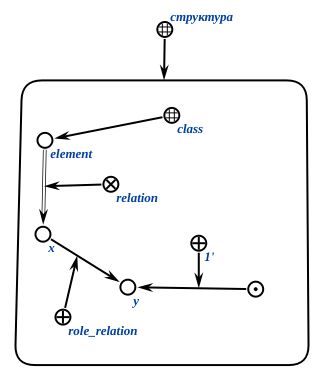
\includegraphics[scale=1]{author/part2/figures/chapter_kb/structure.png}
%	\caption{Представление структуры в SCg}
%	\label{fig:structure_scg}
%\end{figure}

Выделяют следующие классы структур:
\begin{SCn}
	\scnheader{структура}
	\begin{scnrelfromset}{разбиение}
	\scnitem{связная структура}
	\scnitem{несвязная структура}
\end{scnrelfromset}
	\begin{scnrelfromset}{разбиение}
	\scnitem{тривиальная структура}
	\scnitem{нетривиальная структура}
\end{scnrelfromset}
\end{SCn}

\textit{Структуре}, представленной в \textit{SC-коде}, поставим в соответствие орграф, вершинами которого являются \textit{sc-элементы}, а дугами – пары инцидентности, связывающие \textit{sc-коннекторы} с инцидентными им \textit{sc-элементами}, которые являются компонентами указанных \textit{sc-коннекторов}. Если полученный таким способом орграф является связным орграфом, то исходную структуру будем считать \textit{связной структурой}. Если полученный таким способом орграф не является связным орграфом, то исходную структуру будем считать \textit{несвязной структурой}.

Каждая выделяемая структура может выступать в роли либо тривиальной структуры: структуры, которая не содержит связки в качестве элементов, либо в роли нетривиальной структуры: структуры, среди элементов которой есть хотя бы одна связка.

Между структурами можно определять ряд соответствий, таких как гомоморфизм, полиморфизм, автоморфизм, изоморфизм, а также аналогичность структур, что позволяет фиксировать факт наличия некоторой аналогии, сходства и различия некоторых подструктур рассматриваемых структур.

%Пример отношения \textit{аналогичность структур} в SCg представлен на рисунке \textit{\nameref{fig:structure_analogy_scg}}.

%\begin{figure}[H]
%	\centering
%	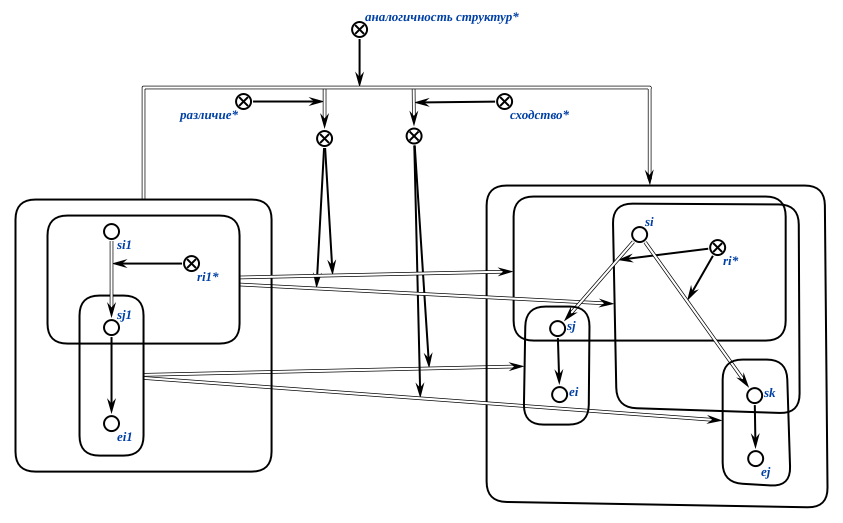
\includegraphics[scale=0.8]{author/part2/figures/chapter_kb/analogy.png}
%	\caption{Пример отношения аналогичность структур в SCg}
%	\label{fig:structure_analogy_scg}
%\end{figure}

\section{Формальная онтология семантических окрестностей}

Для спецификации отдельных сущностей в рамках базы знаний вводиться понятие \textit{семантической окрестности}. Семантическая окрестность представляет собой спецификацию (описание) заданной сущности, знак которой указывается как ключевой элемент этой спецификации.

Набор признаков, по которым можно специфицировать сущности, различен.

Различают полную и базовую семантические окрестности.

\begin{SCn}
	\scnheader{полная семантическая окрестность}
	\scnidtf{полная спецификация некоторой описываемой сущности}
\end{SCn}

Структура \textit{полной семантической окрестности} определяется прежде всего семантической типологией описываемой сущности.
Так, например, для понятия в \textit{полную семантическую окрестность} необходимо включить следующую
информацию (при наличии):
\begin{itemize}
	\item{варианты идентификации на различных внешних языках (sc-идентификаторы)};
	\item{принадлежность некоторой предметной области с указанием роли, выполняемой в рамках этой предметной области};
	\item{теоретико-множественные связи заданного понятия с другими sc-элементами};
	\item{определение или пояснение};
	\item{высказывания, описывающие свойства указанного понятия};
	\item{задачи и их классы, в которых данное понятие является ключевым};
	\item{описание типичного примера использования указанного понятия};
	\item{экземпляры описываемого понятия}.
\end{itemize}

Для понятия, являющегося отношением дополнительно указываются:
\begin{itemize}
	\item {домены};
	\item{область определения};
	\item{схема отношения};
	\item{классы отношений, которым принадлежит описываемое отношение}.
\end{itemize}

\begin{SCn}
	\scnheader{базовая семантическая окрестность}
	\scnidtf{минимально достаточная семантическая окрестность}
	\scnidtf{минимальная спецификация описываемой сущности}
\end{SCn}

Структура \textit{базовой семантической окрестности} определяется прежде всего семантической типологией описываемой сущности. Так, например, для понятия в \textit{базовую семантическую окрестность} необходимо включить следующую  информацию (при наличии):
\begin{itemize}
	\item {варианты идентификации на различных внешних языках (sc-идентификаторы)};
	\item {принадлежность некоторой предметной области с указанием роли, выполняемой в рамках этой предметной области};
	\item{определение или пояснение}.
\end{itemize}

Для понятия, являющегося отношением дополнительно указываются:
\begin{itemize}
	\item {домены};
	\item {область определения};
	\item {описание типичного примера связки указанного отношения (спецификация типичного экземпляра)}.
\end{itemize}

\section{Формальная онтология предметных областей}

Важнейшим этапом разработки баз знаний является процесс выделения описываемых предметных областей и их представления в базе знаний.

Понятие \textit{\textbf{предметной области}} является важнейшим методологическим приемом, позволяющим выделить из всего многообразия исследуемого Мира только определенный класс исследуемых сущностей и только определенное семейство отношений, заданных на указанном классе. То есть осуществляется локализация,
фокусирование внимания только на этом, абстрагируясь от всего остального исследуемого Мира.

Каждой \textit{предметной области} можно поставить в соответствие:
\begin{itemize}
	\item {семейство соответствующих ей онтологий разного вида};
	\item {множество семантических окрестностей, описывающих объекты исследования этой предметной области}.
\end{itemize}


\section{Формальная онтология онтологий}

Для формальной спецификации соответствующей предметной области,
ориентированной на описание свойств и взаимосвязей понятий, входящих в состав указанной предметной области, используется такой вид знаний, как \textit{онтология}.

\begin{SCn}
	\scnheader{онтология}
	\scnidtf{sc-онтология}
	\scnidtf{семантическая спецификация любого знания, имеющего достаточно сложную структуру, любого целостного
		фрагмента базы знаний – предметной области, метода решения сложных задач некоторого класса, описания
		истории некоторого вида деятельности, описания области выполнения некоторого множества действий
		(области решения задач), языка представления методов решения задач и т.д}
\end{SCn}

Онтология включает в себя:
\begin{itemize}
	\item {типологию специфицируемого знания};
	\item{связи специфицируемого знания с другими знаниями};
	\item{спецификацию ключевых понятий, используемых в специфицируемом знании, а также ключевых экземпляров некоторых таких понятий}.
\end{itemize}

Онтологии являются важнейшим видом знаний, обеспечивающих семантическую систематизацию знаний, хранимых в памяти интеллектуальных компьютерных систем (в т.ч. ostis-систем), и, соответственно, семантическую структуризацию баз знаний.

%\input{author/references}
\chapter{Смысловое представление логических формул и высказываний в различного вида логиках}
\chapauthortoc{Шункевич Д.~В.\\Василевская А.~П.\\Орлов М.~К.\\Ивашенко В.~П.}
\label{chapter_logic}

\begin{SCn}
	\begin{scnrelfromlist}{автор}
		\scnitem{Шункевич Д.~В.}
		\scnitem{Василевская А.~П.}
		\scnitem{Орлов М.~К.}
		\scnitem{Ивашенко В.~П.}
	\end{scnrelfromlist}
	
	\bigskip
	
	\scntext{аннотация}{В главе рассмотрено представление логических формул и высказываний как для классических логик и их приложений (прикладных логик), так и представление некоторых понятий неклассических логик.}
	
	\bigskip
	
	\begin{scnrelfromlist}{подраздел}
		\scnitem{\ref{sec_class_logic}~\nameref{sec_class_logic}}
		\scnitem{\ref{sec_applied_logic}~\nameref{sec_applied_logic}}
		\scnitem{\ref{sec_nonclass_logic}~\nameref{sec_nonclass_logic}}
	\end{scnrelfromlist}
	
	\bigskip
	
	\begin{scnrelfromlist}{ключевое понятие}
		\scnitem{логическая формула}
		\scnitem{атомарная логическая формула}
		\scnitem{неатомарная логическая формула}
		\scnitem{замкнутая логическая формула}
		\scnitem{открытая логическая формула}
		\scnitem{высказывание}
		\scnitem{атомарное высказывание}
		\scnitem{неатомарное высказывание}
		\scnitem{фактографическое высказывание}
		\scnitem{нефактографическое высказывание}
		\scnitem{атомарное фактографическое высказывание}
		\scnitem{атомарное нефактографическое высказывание}
		\scnitem{неатомарное нефактографическое высказывание}
		\scnitem{выполнимая логическая формула}
		\scnitem{невыполнимая логическая формула}
		\scnitem{общезначимая логическая формула}
		\scnitem{нейтральная логическая формула}				
		\scnitem{необщезначимая логическая формула}
		\scnitem{логическая формула, равнозначная логической константе}				
		\scnitem{атомарное существование}			
		\scnitem{кратность существования}			
		\scnitem{единственность существования}			
		\scnitem{иррефлексивное слотовое бинарное отношение}
		\scnitem{иррефлексивное неслотовое бинарное отношение}
		\scnitem{рефлексивное слотовое бинарное отношение}
		\scnitem{рефлексивное неслотовое бинарное отношение}
		\scnitem{транзитивное слотовое бинарное отношение}
		\scnitem{транзитивное неслотовое бинарное отношение}
		\scnitem{симметричное слотовое бинарное отношение}
		\scnitem{симметричное неслотовое бинарное отношение}
		\scnitem{антисимметричное слотовое бинарное отношение}
		\scnitem{антисимметричное неслотовое бинарное отношение}
		\scnitem{слотовое бинарное отношение}
		\scnitem{неслотовое бинарное отношение}
		\scnitem{слотовое отношение эквивалентности}
		\scnitem{неслотовое отношение эквивалентности}
		\scnitem{слотовое отношение нестрогого порядка}
		\scnitem{неслотовое отношение нестрогого порядка}
		\scnitem{секвенция}
		\scnitem{метаструктура}
		\scnitem{модальный оператор}
		\scnitem{модальное правило вывода}
		\scnitem{отношение становления структур}
		\scnitem{последовательность мышления}
		\scnitem{немонотонный вывод на конечном sc-множестве посылок}
		\scnitem{выводимое множество}
	\end{scnrelfromlist}
	
	\bigskip
	
	\begin{scnrelfromlist}{ключевое отношение}
		\scnitem{высказывание*}
		\scnitem{неразрешимое высказывание*}
		\scnitem{истинное высказывание*}
		\scnitem{ложное высказывание*}
		\scnitem{подформула*}				
		\scnitem{логическая связка*}				
		\scnitem{конъюнкция*}						
		\scnitem{дизъюнкция*}								
		\scnitem{отрицание*}
		\scnitem{строгая дизъюнкция*}	
		\scnitem{эквиваленция*}
		\scnitem{импликация*}
		\scnitem{если\scnrolesign}										
		\scnitem{то\scnrolesign}												
		\scnitem{квантор*}	
		\scnitem{всеобшность*}	
		\scnitem{существование*}	
		\scnitem{неатомарное существование*}
		\scnitem{нечеткая истинность*}
		\scnitem{конструктивно истинное высказывание*}
		\scnitem{верное высказывание*}
		\scnitem{монотонное бинарное отношение*}
		\scnitem{неискаженное высказывание*}
	\end{scnrelfromlist}

	\begin{scnrelfromlist}{ключевое знание}
		\scnitem{Описание понятия формальной теории}
		\scnitem{Описание понятия утверждения}				
		\scnitem{Описание понятия определение}
	\end{scnrelfromlist}
	
	\bigskip
	
	\begin{scnrelfromlist}{ключевой знак}
		\scnitem{Отношение выводимости}
		\scnitem{Отношение выводимости на конечных множествах}
		\scnitem{Отношение выводимости на конечных множествах полносвязно представленных множеств}
		\scnitem{Отношение выводимости на секвенциях}
	\end{scnrelfromlist}
	
	\bigskip
	
	\begin{scnrelfromlist}{библиографическая ссылка}		
		\scnitem{\scncite{Klini1973}}
		\scnitem{\scncite{Gribomon1990}}
		\scnitem{\scncite{Gribomon1998}}
		\scnitem{\scncite{Dragalin}}
		\scnitem{\scncite{Vagin2008}}
		\scnitem{\scncite{Golenkov2001b}}
		\scnitem{\scncite{Tarasov2007}}
		\scnitem{\scncite{Cintula2011}}		
		\scnitem{\scncite{Ivashenko2014diss}}
		\scnitem{\scncite{Ivashenko2017}}
		\scnitem{\scncite{Letichevskij2003}}
	\end{scnrelfromlist}
	
\end{SCn}

%Перенесено из chapter_logic_productions
%Язык SCL является логическим языком графового типа, используемым ostis-системами. Тексты языка SCL представляют собой однородные семантические сети, являющиеся текстами языка SC. Алфавит языка SCL отдельно не выделяется, так как используется алфавит SC-кода, на котором можно описать любые утверждения, явления, закономерности, программы и любые другие знания. Язык SCL позволяет записывать тексты языка логики высказываний, языка логики предикатов и любых других логических языков. SC-код является метаязыком как для языка SCL, так и для самого себя, то есть он позволяет описывать смысл формул, записанных на SCL. Многие формальные языки, в отличие от SC, недостаточно богаты, чтобы быть метаязыком для самих себя. 

%Одной из важных особенностей SCL является его способность представления текстов языка логики предикатов с учетом семантики этих текстов (высказываний). Язык SCL естественным образом ориентирован на работу в формальной системе языка логики предикатов. Язык SC позволяет записать любые отношения и соответствия в графовом представлении. Значению предиката от некоторого набора sc-переменных соответствует результат операции поиска по шаблону некоторой sc-конструкции (найдена или не найдена), в которую входят sc-константы и/или sc-переменные с соответствующей конфигурацией связей между ними. Подход, основанный на языке SCL для представления формул предоставляет возможность явно не записывать кванторы общности и существования (это не запрещается, однако является излишним). Квантор существования является "встроенным"{} понятием в том смысле, что если некоторый sc-элемент входит в некоторую sc-структуру, то соответствующее понятие существует в этой sc-структуре. Таким образом, квантор существования накладывается автоматически (если иной квантор не наложен явно) на те sc-переменные, которые входят в атомарные логические формулы. Квантор всеобщности накладывается по умолчанию (если иной квантор не наложен явно) на переменные, входящие в связки эквиваленции и импликации в соответствии с денотационной семантикой логических языков.

% Вагин дедукция и обобщения в системах принятия решений
\section{Смысловое представление логических формул и формальных теорий классической логики}
\label{sec_class_logic}
Появление \textit{формальных систем} было обусловлено осознанием того факта, что совершенно различные системы, будь то технические, социальные, экономические или биологические, обладают глубоким сходством. Действительно, каждая конкретная система состоит из каких-то первичных (базовых) элементов, обладающих какими-то свойствами. Затем, исходя из наличия исходных описаний, можно логическим путем вывести описание новых свойств, причем утверждения о наличии исходных или выведенных свойств воспринимаются как истинные на основании смысла определений данных элементов.

\scnkeyword{формальная теория} --- это \textit{множество} \textit{высказываний}, которые считаются истинными в рамках данной \scnkeyword{формальной теории}.

Аксиоматические системы --- это системы с наличием определенного числа исходных заранее выбранных и фиксированных высказываний, называемых аксиомами.

\textit{высказывания} могут быть как фактографическими, так и нефактографическими. Некоторые \textit{высказывания} считаются аксиомами, а другие доказываются на основе других высказываний в рамках этой же \scnkeyword{формальной теории}.

Каждая формальная теория интерпретируется (то есть ее \textit{высказывания} являются истинными) на какой-либо \textit{предметной области}, которая является максимальным из \textit{фактографических высказываний} (их \textit{объединением*}),  входящих в состав этой \scnkeyword{формальной теории}.

Каждой \scnkeyword{формальной теории} соответствует одна \textit{предметная область}, которая входит в нее под атрибутом \textit{предметная область\scnrolesign}.

Каждая \textit{формальная теория} может рассматриваться как \textit{конъюнктивное высказывание}, априори истинное (с чьей-то точки зрения) при интерпретации на соответствующей предметной области.

Каждая \textit{формальная теория} задается \textit{алфавитом}, \textit{формулами}, \textit{аксиомами}, \textit{правилами вывода}.

%\scnrelfrom{источник}{\scncite{Serhievskaya2004}}

\textit{предметная область} является \textit{максимальным фактографическим высказыванием} \textit{формальной теории}, которая интерпретируется на данной \textit{предметной области}.

\textbf{\textit{аксиома}} --- это \textit{высказывание}, истинность которого не требует доказательства в рамках рассматриваемой \textit{формальной теории}.

\textbf{\textit{теорема}} --- это \textit{высказывание}, истинность которого доказывается в рамках рассматриваемой \textit{формальной теории}.

\begin{SCn}
\scnheader{логическая формула}
\begin{scnrelfromset}{разбиение}
	\scnitem{атомарная логическая формула}
	\scnitem{неатомарная логическая формула}
\end{scnrelfromset}
\begin{scnrelfromset}{разбиение}
	\scnitem{замкнутая логическая формула}
	\scnitem{открытая логическая формула}
\end{scnrelfromset}
\end{SCn}
\begin{SCn}
\scnheader{высказывание}
\scnsubset{логическая формула}
\begin{scnrelfromset}{разбиение}
	\scnitem{атомарное высказывание}
	\scnitem{неатомарное высказывание}
\end{scnrelfromset}
\begin{scnrelfromset}{разбиение}
	\scnitem{фактографическое высказывание}
	\begin{scnindent}
		\scnsubset{замкнутая логическая формула}
	\end{scnindent}
	\scnitem{нефактографическое высказывание}
\end{scnrelfromset}
\end{SCn}

Под \textbf{\textit{высказыванием}} понимается некоторая \textit{структура} (в которую входят \textit{sc-константы} из некоторой предметной области и/или \textit{sc-переменные}) или \textit{логическая связка}, которая может трактоваться как истинная или ложная в рамках какой-либо \textit{предметной области}.

Истинность \textbf{\textit{высказывания}} задается путем указания принадлежности знака этого высказывания \textit{формальной теории}, соответствующей данной \textit{предметной области}. Ложность высказывания задается путем указания принадлежности знака \textit{отрицания*} этого высказывания данной \textit{формальной теории}.

Явно указанная непринадлежность \textbf{\textit{высказывания}} \textit{формальной теории} может говорить как о его ложности в рамках данной теории (если это указано рассмотренным выше образом), так и о том, что данное  \textbf{\textit{высказывание}} вообще не рассматривается в данной \textit{формальной теории} (например, использует понятия, не принадлежащие данной \textit{предметной области}).

Одно и то же \textbf{\textit{высказывание}} может быть истинно в рамках одной \textit{формальной теории} и ложно в рамках другой.

%\begin{SCn}
%% Добавить темпоральное высказывание
%\scnheader{высказывание формальной теории\scnrolesign}
%\begin{scnrelfromset}{разбиение}
%	\scnitem{истинное высказывание\scnrolesign}
%	\scnitem{ложное высказывание\scnrolesign}
%%	\scnitem{нечеткое высказывание\scnrolesign}
%	\scnitem{бессмысленное высказывание\scnrolesign}
%\end{scnrelfromset}
%\end{SCn}

%\textbf{\textit{истинное высказывание}} --- высказывание, знак которого принадлежит изучаемой формальной теории.
%Нечеткое высказывание --- высказывание, возможно истинное или ложное в рамках изучаемой формальной теории (высказывание, возможно истинное или ложное в рамках данной формальной теории).
%\textbf{\textit{бессмысленное высказывание}} --- высказывание, не рассматриваемое в рамках данной формальной теории. Высказывание является бессмысленным в рамках заданной формальной теории, если в какое-либо \textit{атомарное высказывание} в его составе (или в само это высказывание, если оно является атомарным) входит какая-либо \textit{sc-константа}, не являющаяся элементом предметной области, описываемой указанной \textit{формальной теорией}.

\begin{SCn}
\scnheader{атомарное высказывание}
\scnsubset{структура}
\begin{scnrelfromset}{разбиение}
	\scnitem{атомарное фактографическое высказывание}
	\scnitem{атомарное нефактографическое высказывание}
\end{scnrelfromset}
\end{SCn}

\textbf{\textit{атомарное высказывание}} --- это \textit{высказывание}, которое не является \textit{неатомарным высказыванием}.

\textbf{\textit{неатомарное высказывание}} --- это \textit{высказывание}, в состав которого входят только знаки \textit{логических формул} или множества связываемых переменных. Следует отметить, что невозможно говорить об истинности либо ложности \textbf{\textit{неатомарного высказывания}} в рамках какой-либо \textit{формальной теории}, в случае, когда невозможно установить истинность либо ложность любого из его элементов в рамках этой же \textit{формальной теории} или интерпретации этих элементов.

Под \textit{фактографическим высказыванием} понимается:
\begin{textitemize}
	\item \textit{атомарное высказывание}, в состав которого не входит ни одна \textit{sc-переменная};
	\item \textit{неатомарное высказывание}, все элементы которого также являются \textbf{\textit{фактографическими высказываниями}}.
\end{textitemize}

\begin{SCn}
\scnheader{высказывание*}
\scnidtf{бинарное ориентированное отношение, каждая \textit{пара} которого связывает (1) знак некоторой \textit{предметной области} и (2) знак некоторого \textit{высказывания}.}
\begin{scnrelfromset}{разбиение}
	\scnitem{ложное высказывание*}
	\scnitem{неразрешимое высказывание*}
%	\begin{scnindent}
%			\scnsuperset{гипотеза}
%	\end{scnindent}}
	\scnitem{истинное высказывание*}	
\end{scnrelfromset}
\end{SCn}

%\scntext{предъявляемое требование}{Все \textit{sc-элементы}, входящие в состав \textit{предметной области}, описываемой высказыванием, (включая и \textit{sc-переменные}, которые, хоть и редко, но могут входить в состав некоторых \textit{предметных областей}) 
%\textit{sc-элементами} для всех высказываний, соответствующих этой \textit{предметной области}.}

\scntext{предъявляемое требование}{Все \textit{sc-константы}, входящие в состав всех \textit{атомарных логических формул}, входящих в состав всех \textit{высказываний}, описывающих некоторую \textit{предметную область} должны входить в состав описываемой \textit{предметной области}.}

\begin{SCn}
\scnheader{следует отличать*}
\begin{scnhaselementset}
	\scnitem{высказывание*}
	\begin{scnindent}
		\scniselement{бинарное ориентированное отношение}
		\scnidtf{быть высказыванием, описывающим заданную предметную область*}
		\begin{scnindent}
			\scntext{сокращение}{быть высказыванием*}
		\end{scnindent}
	\end{scnindent}
	\scnitem{высказывание}
	\begin{scnindent}
		\scnsubset{логическая формула}
		\scnidtf{Второй домен отношения ``быть высказыванием''}
	\end{scnindent}
\end{scnhaselementset}
\end{SCn}

\begin{SCn}
\scnheader{нефактографическое высказывание}
\begin{scnrelfromset}{разбиение}
	\scnitem{атомарное нефактографическое высказывание}
	\scnitem{неатомарное нефактографическое высказывание}
\end{scnrelfromset}
\end{SCn}

Под \textit{нефактографическим высказыванием} понимается:
\begin{textitemize}
	\item \textit{атомарное нефактографическое высказывание}, в состав которого входит хотя бы одна \textit{sc-переменная};
	\item \textit{неатомарное нефактографическое высказывание}, хотя бы один элемент которого является \textbf{\textit{нефактографическим высказыванием}}.
\end{textitemize}

Под \textbf{\textit{атомарным нефактографическим высказыванием}} понимается \textit{атомарное высказывание}, которое является \textit{нефактографическим высказыванием}.

\textbf{\textit{атомарное нефактографическое высказывание}} --- это \textit{нефактографическое высказывание}, которая не является \textit{неатомарным нефактографическим высказыванием}.

\textbf{\textit{атомарная логическая формула}} --- это \textit{логическая формула}, которая не является \textit{неатомарной логической формулой}.

По умолчанию \textbf{\textit{атомарное нефактографическое высказывание}} трактуется как \textit{высказывание} о существовании, то есть наличия в памяти значений, соответствующих всем \textit{sc-переменным}, входящим в состав данной формулы и не попадающих под действие какого-либо другого \textit{квантора} (указанного явно или по умолчанию). Таким образом, на все \textit{sc-переменные}, входящие в состав \textit{атомарного нефактографического высказывания} и не попадающие под действие какого-либо другого \textit{квантора}, неявно накладывается квантор \textit{существования*}.

\begin{SCn}
\scnheader{логическая формула}
\begin{scnrelfromset}{разбиение}
	\scnitem{выполнимая логическая формула}
	\begin{scnindent}
		\begin{scnrelfromset}{разбиение}
			\scnitem{общезначимая логическая формула}
			\scnitem{нейтральная логическая формула}
		\end{scnrelfromset}
	\end{scnindent}
	\scnitem{невыполнимая логическая формула}
\end{scnrelfromset}
\end{SCn}

Под \textbf{\textit{неатомарным нефактографическим высказыванием}} понимается \textit{неатомарное высказывание}, которое является \textit{нефактографическим высказыванием}.

Для того, чтобы рассмотреть типологию \textbf{\textit{неатомарных логических формул}}, будем говорить, что исследуется истинность самой \textbf{\textit{неатомарной логической формулы}} и всех ее \textit{подформул*} в рамках одной и той же \textit{формальной теории}, при этом не важно, какой именно. Также считается, что в рассматриваемой \textit{формальной теории} каждая \textit{подформула*} рассматриваемой \textbf{\textit{неатомарной логической формулы}} в рамках этой \textit{формальной теории} может однозначно трактоваться как либо истинная, либо ложная. В противном случае мы не можем говорить об истинности либо ложности исходной \textbf{\textit{неатомарной логической формулы}} в рамках этой \textit{формальной теории}.

Будем называть \textbf{\textit{подформулой*}} \textit{неатомарной логической формулы} \textbf{\textit{fi}} любую \textit{логическую формулу} \textbf{\textit{fj}}, являющуюся элементом исходной формулы \textbf{\textit{fi}}, а также любую \textbf{\textit{подформулу*}} формулы \textbf{\textit{fj}}.

\begin{SCn}
\scnheader{подформула*}
\scnidtf{частная формула*}
\scniselement{бинарное отношение}
\scniselement{ориентированное отношение}
\scniselement{транзитивное отношение}
%\scnrelfrom{описание примера}{\scnfileitem{figures/sd_logical_formulas/subformula.png}}
\end{SCn}

\begin{figure}[H]
	\caption{Формализация примера подформулы}
	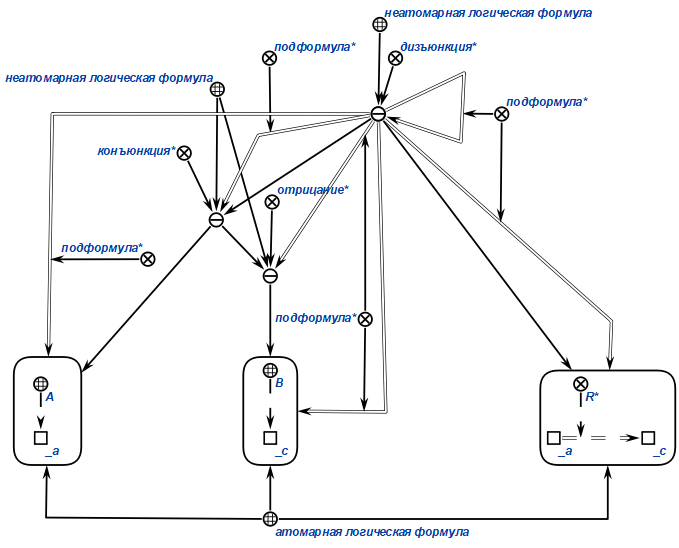
\includegraphics[scale=0.8]{author/part2/figures/logic/subformula.png}
	\label{fig:modus_ponens}
\end{figure}

\textbf{\textit{утверждение}} --- это \textit{семантическая окрестность} некоторой \textit{логической формулы}, в которую входит полный текст этой \textit{логической формулы}, а также факт принадлежности этой \textit{логической формулы} некоторой \textit{формальной теории}.

Знак \textit{логической формулы}, семантическая окрестность которой представляет собой утверждение, является \textit{главным ключевым sc-элементом\scnrolesign} в рамках этого \textbf{\textit{утверждения}}. Знаки понятий соответствующей \textit{предметной области}, которые входят в состав какой-либо \textit{подформулы*} указанной \textit{логической формулы}, будут \textit{ключевыми sc-элементами\scnrolesign} в рамках этого \textbf{\textit{утверждения}}.
	
Полный текст некоторой \textit{логической формулы} включает в себя:
\begin{textitemize}
	\item{знак самой этой \textit{логической формулы}};
	\item{знаки всех ее \textit{подформул*}};
	\item{элементы всех \textit{логических формул}, знаки которых попали в данную структуру;}
	\item{все пары принадлежности, связывающие \textit{логические формулы}, знаки которых попали в данную структуру, с их компонентами.}
\end{textitemize}

Таким образом, факт принадлежности (истинности) логической формулы нескольким \textit{формальным теориям} будет порождать новое утверждение для каждой такой \textit{формальной теории}. Текст \textbf{\textit{утверждения}} входит в состав \textit{логической онтологии}, соответствующей \textit{предметной области}, на которой интерпретируется \textit{главный ключевой sc-элемент\scnrolesign} данного утверждения.

Правило идентификации экземпляров \textbf{\textit{утверждения}} в рамках \textit{Русского языка} именуются по следующим правилам:
\begin{textitemize}
	\item{в начале идентификатора пишется сокращение \textbf{Утв.};}
	\item{далее в круглых скобках через точку с запятой перечисляются основные идентификаторы \textit{ключевых \mbox{sc-элементов}\scnrolesign} данного \textbf{\textit{утверждения}}. Порядок определяется в каждом конкретном случае в зависимости от того, свойства каких из этих \textit{понятий} описывает данное \textbf{\textit{утверждение}} в большей или меньшей степени.}
\end{textitemize}

%\scntext{описание примера}{\textit{Утв. (параллельность*; секущая*)}}
Могут быть исключения для \textbf{\textit{утверждений}}, названия которых закрепились исторически, например, \textit{Теорема Пифагора}, \textit{Аксиома о прямой и точке}.


%\scnrelfrom{описание примера}{\scnfilescg{figures/sd_logical_formulas/statement.png}}
%Утверждение показывает, что соответствующие углы при пересечении параллельных прямых секущей равны.

\textbf{\textit{определение}} --- это \textit{утверждение}, \textit{главным ключевым sc-элементом\scnrolesign} которого является связка \textit{эквиваленции*}, однозначно определяющая некоторое понятие на основе других понятий.

Каждое определение имеет ровно один \textit{ключевой sc-элемент\scnrolesign} (не считая \textit{главного ключевого sc-элемента\scnrolesign}).

Для одного и того же понятия в рамках одной \textit{формальной теории} может существовать несколько \textit{утверждений об эквиваленции*}, однозначно задающих некоторое понятие на основе других, однако только одно такое \textit{утверждение} в рамках этой \textit{формальной теории} может быть отмечено как \textbf{\textit{определение}}. Остальные \textit{утверждения об эквиваленции*} могут трактоваться как \textit{пояснения} данного понятия.

Правило идентификации экземпляров \textbf{\textit{определения}} в рамках \textit{Русского языка} именуются по следующим правилам:
\begin{textitemize}
	\item{в начале идентификатора пишется сокращение \textbf{Опр.};}
	\item{далее в круглых скобках через точку с запятой записывается основной идентификатор  \textit{ключевого sc-элемента\scnrolesign} данного \textbf{\textit{определения}}.}
\end{textitemize}


%\scntext{описание примера}{\textit{Опр. (ромб)}}
%\scnrelfrom{описание примера}{\scnfilescg{figures/sd_logical_formulas/definition.png}}
%\scnnote{Определение показывает, что ромб — это четырехугольник, у которого все стороны равны.}
\begin{SCn}
\scnheader{общезначимая логическая формула}
\scnidtf{тождественно истинная логическая формула}
\scnsubset{выполнимая логическая формула}
\scnsubset{логическая формула, равнозначная логической константе}
\end{SCn}
% Вагин, дедукция и обобщение в системах принятия решений
\textbf{\textit{общезначимая логическая формула}} --- это \textit{логическая формула}, для которой не существует \textit{формальной теории}, в рамках которой она была бы ложной (или имела бы ложную интерпретацию) с учетом истинности и ложности всех ее \textit{подформул*} (или их интерпретаций) в рамках этой же \textit{формальной теории}.

\begin{figure}[H]
\caption{Формализация закона тождества}
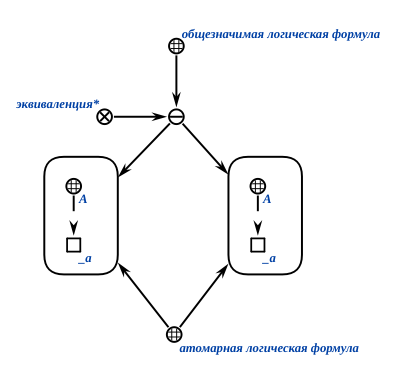
\includegraphics[scale=0.8]{author/part2/figures/logic/valid_formula.png}
\label{fig:valid_formula}
\end{figure}

\begin{SCn}
\scnheader{противоречивая логическая формула}
\scnidtf{тождественно ложная логическая формула}
\scnsubset{невыполнимая логическая формула}
\scnsubset{логическая формула, равнозначная логической константе}
\end{SCn}
% Вагин, дедукция и обобщение в системах принятия решений
\textbf{\textit{противоречивая логическая формула}} --- это \textit{логическая формула}, для которой не существует \textit{формальной теории}, в рамках которой она была бы истинной (или имела бы истинную интерпретацию) с учетом истинности и ложности всех ее \textit{подформул*} (или их интерпретаций) в рамках этой же \textit{формальной теории}.

\begin{figure}[H]
	\caption{Формализация закона противоречия}
	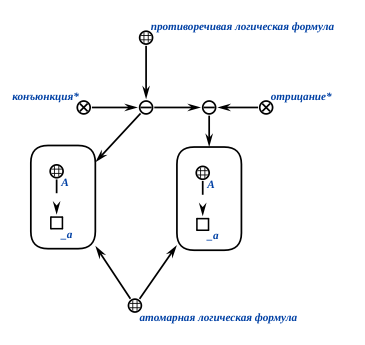
\includegraphics[scale=0.8]{author/part2/figures/logic/contradiction_formula.png}
	\label{fig:contradiction_formula}
\end{figure}

\begin{SCn}
\scnheader{нейтральная логическая формула}
\scnsubset{выполнимая логическая формула}
\end{SCn}

\textbf{\textit{нейтральная логическая формула}} --- это \textit{логическая формула}, для которой существует хотя бы одна \textit{формальная теория}, в рамках которой эта формула ложна (или имеет ложную интерпретацию), и хотя бы одна \textit{формальная теория}, в рамках которой эта формула истинна (или имеет ложную интерпретацию).

\begin{figure}[H]
	\caption{Формализация нейтральной логической формулы}
	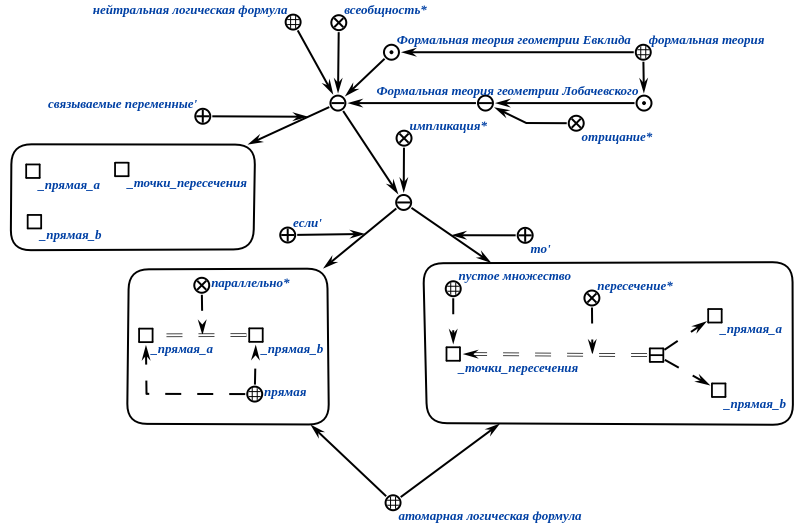
\includegraphics[scale=0.8]{author/part2/figures/logic/neutral_formula.png}
	\label{fig:neutral_formula}
\end{figure}

В \textit{Геометрии Евклида} в плоскости через точку, не лежащую на данной прямой, можно провести одну и только одну прямую, параллельную данной. В \textit{Геометрии Лобачевского} данный постулат является ложным.
В \textit{Сферической геометрии} все прямые пересекаются.

\begin{SCn}
\scnheader{непротиворечивая логическая формула}
\scnidtf{выполнимая логическая формула}
\begin{scnreltoset}{объединение}
	\scnitem{нейтральная логическая формула}
	\scnitem{общезначимая логическая формула}
\end{scnreltoset}
\end{SCn}

\textbf{\textit{непротиворечивая логическая формула}} --- это \textit{логическая формула}, для которой существует хотя бы одна \textit{формальная теория}, в рамках которой эта формула истинна (или имеет истинную интерпретацию).

\begin{SCn}
\scnheader{необщезначимая логическая формула}
%\scnidtf{невыполнимая логическая формула}
\begin{scnreltoset}{объединение}
	\scnitem{нейтральная логическая формула}
	\scnitem{противоречивая логическая формула}
\end{scnreltoset}
\end{SCn}

\textbf{\textit{необщезначимая логическая формула}} --- это \textit{логическая формула}, для которой существует хотя бы одна \textit{формальная теория}, в рамках которой эта формула ложна (или имеет ложную интерпретацию).

\textbf{\textit{логическая формула, равнозначная логической константе}} --- это \textit{логическая формула}, которая является либо только истинной (имеет только истинные интерпретации), либо только ложной (имеет только ложные интерпретации) в рамках всех \textit{формальных теорий}, в которых можно установить ее истинность или ложность.
\textbf{\textit{логическая формула, равнозначная логической константе}} --- это такая \textit{логическая формула}, которая является либо \textit{общезначимой логической формулой}, либо \textit{противоречивой логической формулой}.

\begin{SCn}
\scnheader{логическая связка*}
\scnidtf{неатомарная логическая формула}
\scnidtf{логический оператор*}
\scnidtf{пропозициональная связка*}
\scniselement{класс связок разной мощности}
\scnrelto{семейство подмножеств}{неатомарное высказывание}
\end{SCn}

\textbf{\textit{логическая связка*}} --- это отношение (класс связок), связками которого являются \textit{высказывания}, а областью определения которого является множество \textit{высказываний}, при этом само это отношение и некоторые его подмножества могут быть \textit{классами связок разной мощности}.

\begin{SCn}
\scnheader{конъюнкция*}
\scnidtf{логическое и*}
\scnidtf{логическое умножение*}
\scnsubset{логическая связка*}
\scniselement{неориентированное отношение}
\scniselement{класс связок разной мощности}
\scniselement{неунарное отношение}
\scnrelfrom{область определения}{логическая формула}
\end{SCn}

\textbf{\textit{конъюнкция*}} --- это множество конъюнктивных \textit{логических формул}, каждая из которых истинна (имеет истинные интерпретации) в рамках некоторой \textit{формальной теории} только в том случае, когда все ее компоненты истинны (имеют только соответствующие истинные интерпретации) в рамках этой же \textit{формальной теории}. 
%\textit{конъюнкция*} атомарных формул может быть представлена атомарной формулой, полученной путем объединения исходных атомарных формул.

\begin{figure}[H]
	\caption{Формализация примера конъюнкции}
	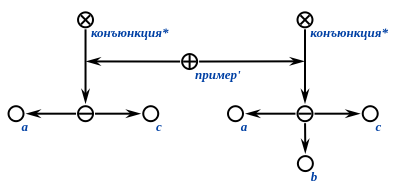
\includegraphics[scale=0.8]{author/part2/figures/logic/conjunction.png}
	\label{fig:conjunction}
\end{figure}

%logically incorrect figure
%\begin{figure}[H]
%	\caption{Формализация примера конъюнкции в геометрии}
%	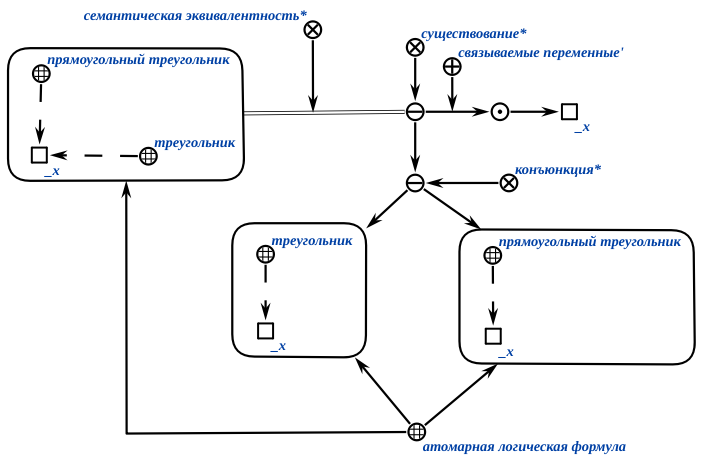
\includegraphics[scale=0.8]{author/part2/figures/logic/conjunction_triangles.png}
%	\label{fig:conjunction_triangles}
%	\scnexplanation{Данные конструкции эквивалентны по принципу $\exists x T(x) \land \exists x PT(x) \ \Longrightarrow \ \exists x (T(x) \land PT(x))$}
%\end{figure}

\begin{SCn}
\scnheader{дизъюнкция*}
\scnidtf{логическое или*}
\scnidtf{логическое сложение*}
\scnidtf{включающее или*}
\scnsubset{логическая связка*}
\scniselement{неориентированное отношение}
\scniselement{класс связок разной мощности}
\scniselement{неунарное отношение}
\scnrelfrom{область определения}{логическая формула}
\end{SCn}

\textbf{\textit{дизъюнкция*}} --- это множество дизъюнктивных \textit{логических формул}, каждая из которых истинна (имеет истинные интерпретации) в рамках некоторой \textit{формальной теории} только в том случае, когда хотя бы один его компонент является истинным (имеет соответствующую истинную интерпретацию) в рамках этой же \textit{формальной теории}.

Следует отметить, что каждая конъюнктивная и дизъюнктивная формула представляют собой связку (множество) своих непосредственных подформул, причем эти множества могут быть равными, однако, такие множества будем полагать различными, так как одно множество будет представлять конъюнкцию, а другое -- дизъюнкцию. Наличие равных, но различных множеств не допускается в классической математике, которая основывается, в том числе, на абстракции обобщения (все равные множества (абстракции) -- тождественны). Однако, такие множества могут существовать в неклассических математических моделях. Таким образом, в рамках языка SC будем использовать неклассическую математическую модель для представления логических формул классической математической логики.

\begin{figure}[H]
	\caption{Формализация примера дизъюнкции}
	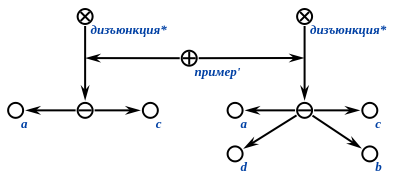
\includegraphics[scale=0.8]{author/part2/figures/logic/disjunction.png}
	\label{fig:disjunction}
\end{figure}

\begin{SCn}
\scnheader{отрицание*}
\scnsubset{логическая связка*}
\scnsubset{синглетон}
\scniselement{унарное отношение}
\scnrelfrom{область определения}{логическая формула}
\end{SCn}

\textbf{\textit{отрицание*}} --- это множество \textit{логических формул} об отрицании, каждое из которых истинно (имеет истинную интерпретацию) в рамках некоторой \textit{формальной теории} только в том случае, когда его единственный элемент является ложным (имеет ложную эту же интерпретацию) в рамках этой же \textit{формальной теории}.

\begin{figure}[H]
	\caption{Формализация примера отрицания}
	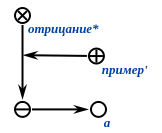
\includegraphics[scale=0.8]{author/part2/figures/logic/negation.png}
	\label{fig:negation}
\end{figure}

\begin{SCn}
\scnheader{строгая дизъюнкция*}
%\scnidtf{сложение по модулю 2*}
\scnidtf{исключающее или*}
\scnidtf{альтернатива*}
\scnsubset{логическая связка*}
\scniselement{неориентированное отношение}
\scniselement{класс связок разной мощности}
\end{SCn}

\textbf{\textit{строгая дизъюнкция*}} --- это множество строго дизъюнктивных \textit{логических формул}, каждое из которых истинно в рамках некоторой \textit{формальной теории} только в том случае, когда ровно один его компонент является истинным (имеет соответствующую истинную интерпретацию) в рамках этой же \textit{формальной теории}.

\begin{figure}[H]
	\caption{Формализация примера строгой дизъюнкции в геометрии}
	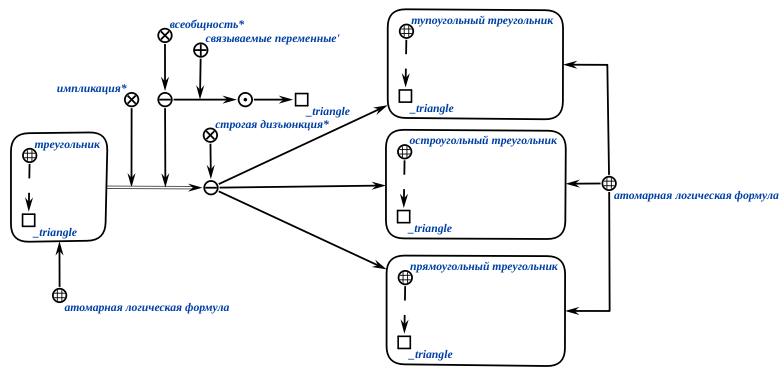
\includegraphics[scale=0.8]{author/part2/figures/logic/strict_disjunction_triangle.png}
	\label{fig:strict_disjunction_triangle}
\end{figure}
	\scnexplanation{Данная неатомарная логическая формула содержит следующую информацию: для любых переменных \_triangle если \_triangle является треугольником, то \_triangle является или тупоугольным треугольником, или остроугольным треугольником, или прямоугольным треугольником.}

\begin{figure}[H]
	\caption{Формализация примера строгой дизъюнкции}
	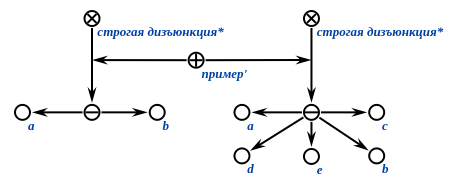
\includegraphics[scale=0.8]{author/part2/figures/logic/strictDisjunction.png}
	\label{fig:strict_disjunction}
\end{figure}

\textbf{\textit{строгая дизъюнкция*}} может быть представлена как \textit{дизъюнкция} \textit{конъюнкции} \textit{отрицания} первой логической формулы и второй логической формулы и \textit{конъюнкции} первой логической формулы и \textit{отрицания} второй логической формулы. Также она может быть представлена и в виде \textit{конъюнкции} \textit{дизъюнкций} двух логических формул и их \textit{отрицаний}.

\begin{figure}[H]
	\caption{Формализация примера строгой дизъюнкции}
	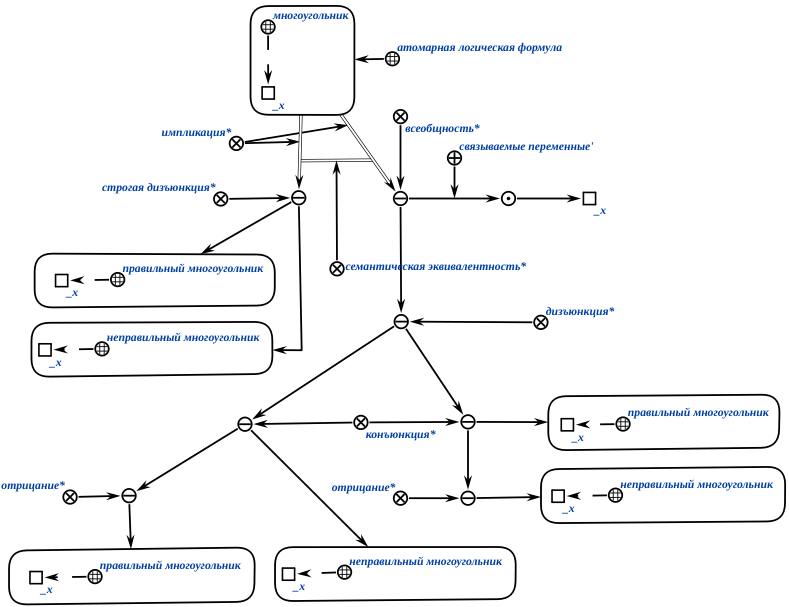
\includegraphics[scale=0.8]{author/part2/figures/logic/strict_disjunction_representation.png}
	\label{fig:strict_disjunction_representation}
\end{figure}

\begin{SCn}
\scnheader{импликация*}
\scnidtf{логическое следование*}
\scnsubset{логическая связка*}
\scniselement{бинарное отношение}
\scniselement{ориентированное отношение}
\scnrelfrom{область определения}{логическая формула}
\end{SCn}

\textbf{\textit{импликация*}} --- это множество импликативных \textit{логических формул}, каждая из которых состоит из посылки (первый компонент \textit{высказывания}) и следствия (второй компонент \textit{высказывания}).

Каждое импликативное \textit{высказывание} ложно в рамках некоторой \textit{формальной теории} в том случае, когда его посылка истинна, а заключение ложно в рамках этой же \textit{формальной теории}. В других случаях такое \textit{высказывание} истинно.

По умолчанию на все переменные, входящие в обе части высказывания об \textbf{\textit{импликации*}} (или хотя бы одну из \textit{подформул*} каждой части) неявно накладывается квантор \textit{всеобщности*}, при условии, что эти переменные не связаны другим \textit{квантором}, указанным явно.

\begin{figure}[H]
\caption{Формализация примера импликации}
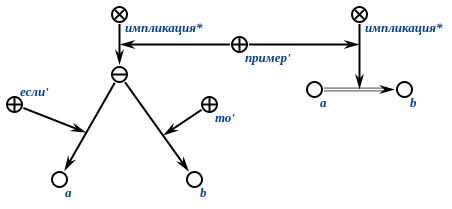
\includegraphics[scale=0.8]{author/part2/figures/logic/implication.png}
\label{fig:implication}
\end{figure}

\textbf{\textit{импликация*}} может быть представлена как \textit{дизъюнкция} \textit{отрицания} первой логической формулы и второй логической формулы или же как \textit{отрицание} \textit{конъюнкции} первой логической формулы и \textit{отрицания} второй логической формулы.

\begin{figure}[H]
	\caption{Формализация примера импликации}
	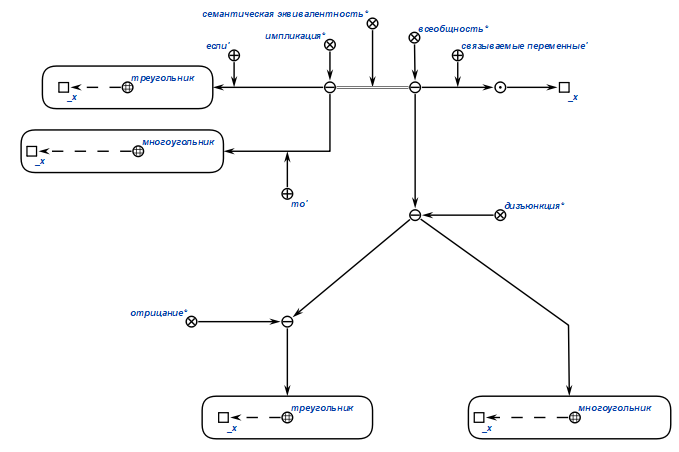
\includegraphics[scale=0.8]{author/part2/figures/logic/implication_representation.png}
	\label{fig:implication_representation}
\end{figure}

\begin{figure}[H]
	\caption{Формализация примера импликации}
	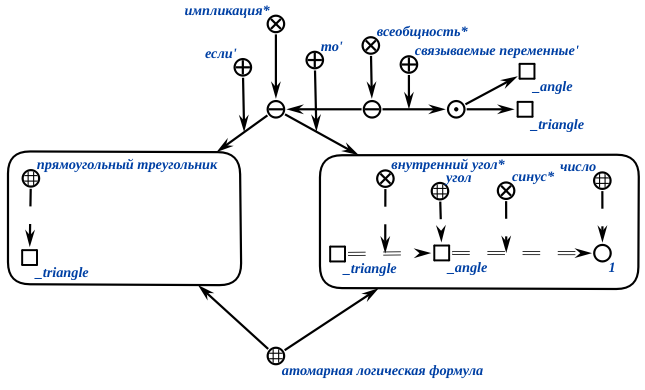
\includegraphics[scale=0.8]{author/part2/figures/logic/implication_triangle.png}
	\label{fig:implication_triangle}
\end{figure}
\vspace{-2\baselineskip}
\scnexplanation{Данная неатомарная логическая формула содержит следующую информацию: для любых переменных \_triangle и \_angle если \_triangle является прямоугольным треугольником, то синус его внутреннего угла \_angle равен единице.}

\begin{SCn}
\scnheader{если\scnrolesign}
\scnidtf{посылка\scnrolesign}
\scnsubset{1\scnrolesign}
\scniselement{ролевое отношение}
\end{SCn}

\textbf{\textit{если\scnrolesign}} --- это \textit{ролевое отношение}, используемое в связках \textit{импликации*} для указания посылки.

\begin{SCn}
\scnheader{то\scnrolesign}
\scnidtf{следствие\scnrolesign}
\scnsubset{2\scnrolesign}
\scniselement{ролевое отношение}
\end{SCn}

\textbf{\textit{то\scnrolesign}} --- это \textit{ролевое отношение}, используемое в связках \textit{импликации*} для указания следствия.

\begin{SCn}
\scnheader{эквиваленция*}
\scnidtf{эквивалентность*}
\scnsubset{логическая связка*}
\scniselement{бинарное отношение}
\scniselement{неориентированное отношение}
\scnrelfrom{область определения}{логическая формула}
\end{SCn}

\textbf{\textit{эквиваленция*}} --- это множество \textit{логических формул} об эквивалентности, каждое из которых истинно (имеет истинную интерпретацию) в рамках некоторой \textit{формальной теории} только в тех случаях, когда оба его компонента одновременно либо истинны (имеют соответствующие истинные интерпретации) в рамках этой же \textit{формальной теории}, либо ложны (имеют соответствующие ложные интерпретации).

По умолчанию на все переменные, входящие в обе части высказывания об \textbf{\textit{эквиваленции*}} (или хотя бы одну из \textit{подформул*} каждой части) неявно накладывается квантор \textit{всеобщности*}, при условии, что эти переменные не связаны другим \textit{квантором}, указанным явно.

\begin{figure}[H]
	\caption{Формализация примера эквиваленции}
	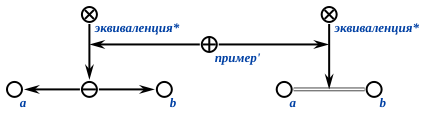
\includegraphics[scale=0.8]{author/part2/figures/logic/equivalent.png}
	\label{fig:equivalent}
\end{figure}

\textbf{\textit{эквиваленция*}} двух логических формул может быть представлена как \textit{дизъюнкция} \textit{конъюнкции} этих двух логических формул и \textit{конъюнкции} \textit{отрицаний} этих двух логических формул.

\begin{figure}[H]
	\caption{Формализация примера эквиваленции}
	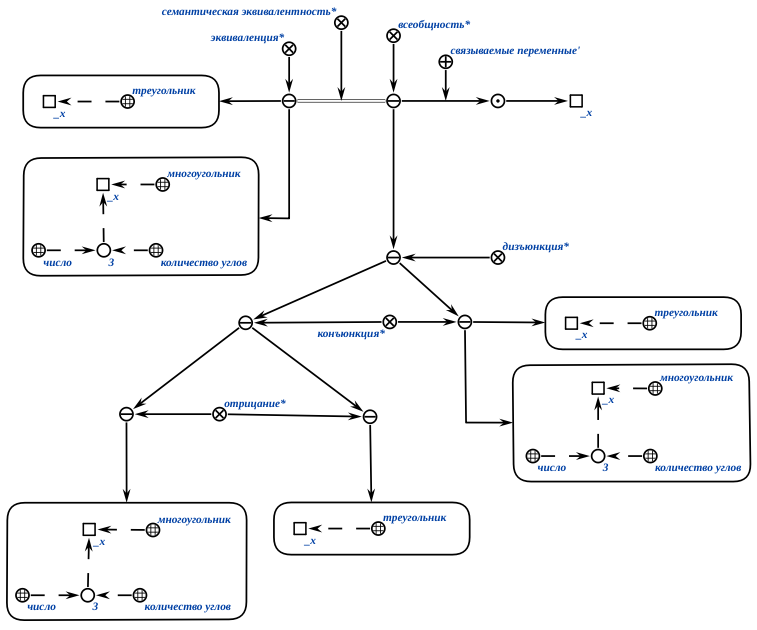
\includegraphics[scale=0.8]{author/part2/figures/logic/equivalence_representation.png}
	\label{fig:equivalence_representation}
\end{figure}

\begin{SCn}
\scnheader{квантор}
\scnsubset{логическая связка*}
\end{SCn}

\textbf{\textit{квантор}} — это \textit{отношение}, каждая связка которого истинна (или имеет истинную интерпретацию) при выполнении дополнительных условий, связанных с некоторыми из переменных, входящих в состав \textit{логических формул}, входящих в ее состав.

Будем говорить, что переменные связаны \textbf{\textit{квантором}} или попадают под область действия данного \textbf{\textit{квантора}} (имея в виду конкретную связку конкретного \textbf{\textit{квантора}}).

В состав каждой связки каждого \textbf{\textit{квантора}} входит \textit{атомарная формула}, являющаяся \textit{тривиальной структурой}, в которой перечислены переменные, связанные данным \textbf{\textit{квантором}}.

\begin{SCn}
\scnheader{всеобщность*}
\scnidtf{квантор всеобщности*}
\scnidtf{квантор общности*}
\scniselement{квантор}
\scniselement{ориентированное отношение}
\scniselement{класс связок разной мощности}
\end{SCn}

\textbf{\textit{всеобщность*}} --- это \textit{квантор}, для каждой связки которого, истинной в рамках некоторой \textit{формальной теории} (или имеющей истинную интерпретацию), выполняется следующее утверждение: все формулы, входящие в состав этой связки имеют соответствующую истинную интерпретацию в рамках этой же \textit{формальной теории} при всех (любых) возможных значениях всех элементов множества \textit{связываемых переменных\scnrolesign} входящего в эту связку.

Каждая связка \textit{квантора} \textbf{\textit{всеобщность*}} может быть представлена как \textit{конъюнкция*} (потенциально бесконечная) исходных \textit{логических формул}, входящих в состав этой связки, в каждой из которых все \textit{связанные переменные\scnrolesign} заменены на их возможные значения.

Квантор \textbf{\textit{всеобщности*}} зачастую обозначается ``$\forall$'' и читается как ``для всех'', ``для каждого'', ``для любого'' или ``все'', ``каждый'', ``любой''.

\begin{figure}[H]
\caption{Формализация примера всеобщности}
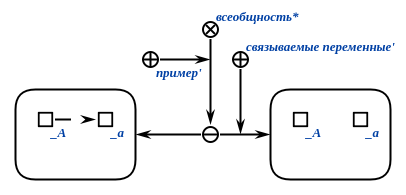
\includegraphics[scale=0.8]{author/part2/figures/logic/universality.png}
\label{fig:universality}
\end{figure}

\begin{SCn}
\scnheader{формула существования}
\scnidtf{существование*}
\begin{scnrelfromset}{разбиение}
	\scnitem{атомарное существование}
	\scnitem{неатомарное существование*}
\end{scnrelfromset}

\scnheader{неатомарное существование*}
\scnidtf{квантор неатомарного существования*}
\scniselement{квантор}
\scniselement{ориентированное отношение}
\scniselement{класс связок разной мощности}
\end{SCn}

\textbf{\textit{неатомарное существование*}} --- это \textit{квантор}, для каждой связки которого, истинной в рамках некоторой \textit{формальной теории} (или имеющей истинную интерпретацию), выполняется следующее утверждение: существуют значения всех элементов множества \textit{связываемых переменных\scnrolesign} входящего в эту связку, такие, что все формулы, входящие в состав этой связки имеют соответствующую истинную интерпретацию в рамках этой же \textit{формальной теории}.

Каждая связка \textit{квантора} \textbf{\textit{неатомарное существование*}} может быть представлена как \textit{дизъюнкция*} (потенциально бесконечная) исходных \textit{логических формул}, входящих в состав этой связки, в каждой из которых все \textit{связанные переменные\scnrolesign} заменены на их возможные значения.

Квантор \textbf{\textit{существования*}} зачастую обозначается ``$\exists$'' и читается как ``существует'', ``для некоторого'', ``найдется''.

\begin{figure}[H]
\caption{Формализация примера неатомарного существования}
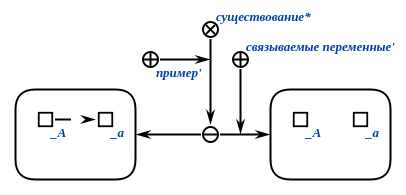
\includegraphics[scale=0.8]{author/part2/figures/logic/non_atomicExistence.png}
\label{fig:non_atomic_existence}
\end{figure}

\begin{SCn}
\scnheader{число значений переменной}
\scniselement{параметр}
\end{SCn}

Каждый элемент \textit{параметра} \textbf{\textit{число значений переменной}} представляет собой класс ориентированных пар, первым компонентом которых является знак \textit{логической формулы}, вторым --- \textit{sc-переменная}, имеющая в рамках данной \textit{логической формулы} ограниченное известное число значений, при которых данная формула является истинной в рамках соответствующей \textit{формальной теории}.

Отметим, что в случае \textit{атомарной логической формулы} каждая такая связка связывает знак формулы и знак принадлежащей ей \textit{sc-переменной}, то есть является, по сути, частным случаем пары принадлежности. В случае \textit{неатомарной логической формулы} указанная \textit{sc-переменная} может принадлежать любой из \textit{подформул*} исходной формулы.

\textit{измерением*} значения параметра \textbf{\textit{число значений переменной}} является некоторое \textit{число}, задающее количество значений \textit{sc-переменных} в рамках \textit{логической формулы}.

\begin{SCn}
\scnheader{кратность существования}
\scniselement{параметр}
\scnrelfrom{область определения параметра}{формула существования}
\scnhaselement{единственное существование}
\end{SCn}

Каждый элемент \textit{параметра} \textbf{\textit{кратность существования}} представляет собой класс логических \textit{формул существования}, для которых  при интерпретации на соответствующей \textit{предметной области} существует ограниченное общее для всех таких формул число комбинаций значений переменных, при которых указанные формулы являются истинными в рамках соответствующей \textit{формальной теории}.
\textit{измерением*} каждого значения \textbf{\textit{кратности существования}} является некоторое \textit{число}, задающее количество таких комбинаций.

\begin{SCn}
\scnheader{единственное существование}
\scnidtf{однократное существование}
\scnidtf{формула существования и единственности}
\end{SCn}

Единственное существование зачастую обозначается ``$\exists!$'' и читается как ``существует и единственный''.

\begin{SCn}
\scnheader{логическая формула и единственность}
\scnsubset{логическая формула}
\scnsubset{единственное существование}
\end{SCn}

Каждый элемент множества \textbf{\textit{логическая формула и единственность}} представляет собой \textit{логическую формулу} (\textit{атомарную} или \textit{неатомарную}), для которой дополнительно уточняется, что при ее интерпретации на некоторой предметной области существует только один набор значений переменных, входящих в эту формулу (или ее \textit{подформулы*}), при котором указанная логическая формула истинна в рамках \textit{формальной теории}, в которую входит данная \textit{предметная область}.


%\scnfilescg{figures/sd_logical_formulas/unique_existance.png}
%Данная формула показывает, что в рамках формальной теории геометрии Евклида существует только один прямоугольный треугольник с некоторым периметром, являющийся равнобедренным.

\textbf{\textit{связываемые переменные\scnrolesign}} --- это \textit{ролевое отношение}, которое связывает связку конкретного \textit{квантора} с множеством переменных, которые связаны этим квантором.

\textbf{\textit{открытая логическая формула}} --- это \textit{логическая формула}, в рамках которой (и всех ее \textit{подформул*}) существует хотя бы одна переменная, не связанная никаким \textit{квантором}.

\textbf{\textit{замкнутая логическая формула}} --- это \textit{логическая формула}, в рамках которой (и всех ее \textit{подформул*}) не существует переменных, не связанных каким-либо \textit{квантором}.

%\scnheader{Примеры неатомарных логических формул}
%\scneqtoset{\scgfileitem{figures/sd_logical_formulas/example_line_segment_sum.png}\\
%\scnrelfrom{описание примера}{
%\scnfilescg{figures/sd_logical_formulas/example_line_segment_sum_note.png}}
%\scnexplanation{AB+BC=AC}
%;
%\scgfileitem{figures/sd_logical_formulas/example_line_segment_diff.png}\\
%\scnrelfrom{описание примера}{
%\scnfilescg{figures/sd_logical_formulas/example_line_segment_diff_note.png}}
%\scnexplanation{AB-AC=CB}

\section{Смысловое представление логических формул и высказываний в прикладных логиках}
\label{sec_applied_logic}
\begin{SCn}
	\begin{scnrelfromlist}{ключевое понятие}
		\scnitem{иррефлексивное слотовое бинарное отношение}
		\scnitem{иррефлексивное неслотовое бинарное отношение}
		\scnitem{рефлексивное слотовое бинарное отношение}
		\scnitem{рефлексивное неслотовое бинарное отношение}
		\scnitem{транзитивное слотовое бинарное отношение}
		\scnitem{транзитивное неслотовое бинарное отношение}
		\scnitem{симметричное слотовое бинарное отношение}
		\scnitem{симметричное неслотовое бинарное отношение}
		\scnitem{антисимметричное слотовое бинарное отношение}
		\scnitem{антисимметричное неслотовое бинарное отношение}
		\scnitem{монотонное бинарное отношение*}
		\scnitem{отношение порядка монотонного отношения\scnrolesign}
		\scnitem{монотонное бинарное отношение\scnrolesign}
		\scnitem{монотонное слотовое бинарное отношение*}
		\scnitem{монотонное неслотовое бинарное отношение*}
		\scnitem{слотовое бинарное отношение}
		\scnitem{неслотовое бинарное отношение}
		\scnitem{слотовое отношение эквивалентности}
		\scnitem{неслотовое отношение эквивалентности}
		\scnitem{слотовое отношение нестрогого порядка}
		\scnitem{неслотовое отношение нестрогого порядка}
		\scnitem{секвенция}
		\scnitem{метаструктура}
		\scnitem{модальный оператор}
		\scnitem{модальное правило вывода}
		\scnitem{отношение становления структур}
		\scnitem{последовательность мышления}
		\scnitem{последовательность рационального мышления}
		\scnitem{последовательность иррационального мышления}
		\scnitem{последовательность рационального мышления классической логики}
		\scnitem{последовательность рационального дедуктивного мышления классической логики}
		\scnitem{последовательность рационального дедуктивного мышления классической логики на конечных sc-множествах}
		\scnitem{последовательность классического рационального дедуктивного познания}
	\end{scnrelfromlist}
\end{SCn}
\begin{SCn}
	\begin{scnrelfromlist}{ключевой знак}
		\scnitem{Отношение выводимости}
		\scnitem{Отношение выводимости на конечных множествах}
		\scnitem{Отношение выводимости на конечных множествах полносвязно представленных множеств}
		\scnitem{Отношение выводимости на секвенциях}
	\end{scnrelfromlist}
\end{SCn}

Прикладные логики (см. \scncite{Klini1973}, \scncite{Gribomon1990}, \scncite{Dragalin}, \scncite{Vagin2008}, \scncite{Gribomon1998}, \scncite{Golenkov2001b}) рассматривают приложения классической логики к абстрактным и предметным областям, описывающим действительность: логические теории об отношениях равенства и порядка (см. \scncite{Klini1973}, \scncite{Gribomon1990}), логические теории арифметики (см. \scncite{Klini1973}), логические теории времени (см. \scncite{Gribomon1998}, \scncite{Vagin2008}), логические теории доказательств (см. \scncite{Dragalin}, \scncite{Klini1973}), теории графов и геометрические теории (см. \scncite{Golenkov2001b}), теории природных и социальных систем (см. \scncite{Gribomon1990}).

Классификация логических теорий соответствует классификации предметных областей.
Рассмотрим некоторые понятия и примеры, которые рассматриваются в рамках прикладных логик.

\begin{SCn}
	\scnheader{слотовое бинарное отношение}
	\scnnote{Слотовое бинарное отношение --- слотовое sc-отношение, являющееся множеством.}
\end{SCn}
\begin{SCn}
	\scnheader{неслотовое бинарное отношение}
	\scnnote{Неслотовое бинарное отношение --- бинарное sc-отношение, являющееся множеством, но не являющееся слотовым sc-отношением.}
\end{SCn}
\begin{SCn}
	\scnheader{иррефлексивное слотовое бинарное отношение}
	\scnsubset{иррефлексивное бинарное отношение}
	\scnnote{Иррефлексивное слотовое бинарное отношение --- слотовое (бинарное) отношение, любая связка которого не является связкой,обозначенной петлевой дугой (дугой с совпадающим началом и концом).}
\end{SCn}
\begin{SCn}
	\scnheader{иррефлексивное неслотовое бинарное отношение}
	\scnsubset{иррефлексивное бинарное отношение}
	\scnnote{Иррефлексивное неслотовое бинарное отношение --- неслотовое бинарное sc-отношение, для любой связки которого ее различные принадлежности являются принадлежностями различных элементов.}
\end{SCn}
\begin{SCn}
	\scnheader{рефлексивное слотовое бинарное отношение}
	\scnsubset{рефлексивное бинарное отношение}
	\scnnote{Рефлексивное слотовое бинарное отношение --- слотовое бинарное sc-отношение, для любого элемента связки которого найдется связка, обозначенная петлевой дугой (дугой с совпадающим началом и концом).}
\end{SCn}
\begin{SCn}
	\scnheader{рефлексивное неслотовое бинарное отношение}
	\scnsubset{рефлексивное бинарное отношение}
	\scnnote{Рефлексивное неслотовое бинарное отношение --- неслотовое бинарное sc-отношение, для любого элемента связки которого найдется связка, имеющая две различные принадлежности этого элемента.}
\end{SCn}
\begin{SCn}
	\scnheader{транзитивное слотовое бинарное отношение}
	\scnsubset{транзитивное бинарное отношение}
	\scnnote{Транзитивное слотовое бинарное отношение --- слотовое бинарное отношение, для любых двух связок которого, конец одной из которых является началом второй, существует связка началом которой является начало первой связки, а концом является конец второй связки.}
\end{SCn}
\begin{SCn}
	\scnheader{транзитивное неслотовое бинарное отношение}
	\scnsubset{транзитивное бинарное отношение}
	\scnnote{Транзитивное неслотовое бинарное отношение --- неслотовое бинарное отношение, для которого существует ролевое отношение, первым доменом которого является это бинарное отношение такое, что для любых двух связок этого бинарного отношения, принадлежность элемента одной из которых не принадлежит этому ролевому отношению, а принадлежность этого же элемента второй связке принадлежит этому ролевому отношению, существует связка с принадлежностью элемента, принадлежащей ролевому отношению, принадлежность которого первой связке принадлежит ролевому отношению, и с принадлежностью элемента, не принадлежащей ролевому отношению, принадлежность которого второй связке не принадлежит этому ролевому отношению.}
\end{SCn}
\begin{SCn}
	\scnheader{симметричное слотовое бинарное отношение}
	\scnsubset{симметричное бинарное отношение}
	\scnnote{Симметричное слотовое бинарное отношение --- слотовое бинарное отношение, для любой связки которого существует связка, конец которой является началом первой связки, а начало --- ее концом (то есть эти связки обозначены встречными дугами).}
\end{SCn}
\begin{SCn}
	\scnheader{симметричное неслотовое бинарное отношение}
	\scnsubset{симметричное бинарное отношение}
	\scnnote{Симметричное неслотовое бинарное отношение --- неслотовое бинарное отношение, для которого существует ролевое отношение, первым доменом которого является это бинарное отношение, для любой связки которого существует связка с принадлежностью элемента первой связке, принадлежащая ролевому отношению, принадлежность которого второй связке не принадлежит этому ролевому отношению, и с принадлежностью элемента первой связке, не принадлежащая ролевому отношению, принадлежность которого второй связке принадлежит этому же ролевому отношению.}
\end{SCn}
\begin{SCn}
	\scnheader{антисимметричное слотовое бинарное отношение}
	\scnsubset{антисимметричное бинарное отношение}
	\scnnote{Антисимметричное слотовое бинарное отношение --- слотовое бинарное отношение, для любой связки которого у которой различным начало и конец не существует связки, конец которой является началом первой связки, а начало --- ее концом (то есть эти связки обозначены встречными дугами).}
\end{SCn}
\begin{SCn}
	\scnheader{антисимметричное неслотовое бинарное отношение}
	\scnsubset{антисимметричное бинарное отношение}
	\scnnote{Антисимметричное неслотовое бинарное отношение --- неслотовое бинарное отношение, для которого существует ролевое отношение, первым доменом которого является это бинарное отношение, для любой связки которого не существует связки с принадлежностью элемента первой связке, принадлежащая ролевому отношению, принадлежность которого второй связке не принадлежит этому ролевому отношению, и с принадлежностью другого элемента первой связке, не принадлежащая ролевому отношению, принадлежность которого второй связке принадлежит этому же ролевому отношению.}
\end{SCn}
\begin{SCn}
	\scnheader{монотонное слотовое бинарное отношение*}
	\scnsubset{монотонное бинарное отношение*}
	\scnnote{Монотонное слотовое бинарное отношение* --- слотовое бинарное отношение по отношению к отношению порядка, если есть связка этого бинарного отношения, то для любой его связки, начало которой связано связкой этого отношения порядка с началом первой, найдется третья связка бинарного отношения, начало которой совпадает с началом втором связки, а конец совпадает с концом первой.}
\end{SCn}
\begin{SCn}
	\scnheader{отношение порядка монотонного отношения\scnrolesign}
	\scnrelfrom{первый домен}{монотонное бинарное отношение*}
	\scnrelfrom{второй домен}{отношение порядка}
\end{SCn}
\begin{SCn}
	\scnheader{монотонное бинарное отношение\scnrolesign}
	\scnrelfrom{первый домен}{монотонное бинарное отношение*}
	\scnrelfrom{второй домен}{монотонное бинарное отношение}
\end{SCn}
\begin{SCn}
	\scnheader{монотонное неслотовое бинарное отношение*}
	\scnsubset{монотонное бинарное отношение*}
	\scnnote{Монотонное неслотовое бинарное отношение* --- неслотовое бинарное отношение по отношению к отношению порядка, для которого существует ролевое отношение, первым доменом которого является это бинарное отношение, такое, что если есть связка этого бинарного отношения, то для любой его связки элемент принадлежащий ей под этим ролевым отношением в отличие от другого связан связкой этого отношения порядка с элементом принадлежащим первой связки под этим же ролевым отношением, в отличие от другого элемента первой связки, найдется третья связка бинарного отношения такая, что элемент, принадлежащий ей под ролевым отношением, принадлежит под этим же ролевым отношением второй связке, а элемент, принадлежащий не под ролевым отношением третьей связке, принадлежит не под ролевым отношением первой связке.}
\end{SCn}
\begin{SCn}
	\scnheader{слотовое отношение эквивалентности}
	\scnsubset{sc-отношение эквивалентности}
	\scnnote{Слотовое отношение эквивалентности --- слотовое транзитивное бинарное отношение, которое является слотовым рефлексивным и симметричным отношением.}
\end{SCn}
\begin{SCn}
	\scnheader{неслотовое отношение эквивалентности}
	\scnsubset{sc-отношение эквивалентности}
	\scnnote{Неслотовое отношение эквивалентности --- неслотовое транзитивное бинарное отношение, которое является неслотовым рефлексивным и симметричным отношением (по соответствующим доменам).}
\end{SCn}
\begin{SCn}
	\scnheader{слотовое отношение нестрогого порядка}
	\scnsubset{sc-отношение нестрогого порядка}
	\scnnote{Слотовое отношение нестрогого порядка --- транзитивное бинарное отношение, которое является рефлексивным и антисимметричным.}
\end{SCn}
\begin{SCn}
	\scnheader{неслотовое отношение нестрогого порядка}
	\scnsubset{sc-отношение нестрогого порядка}
	\scnnote{Неслотовое отношение нестрогого порядка --- транзитивное бинарное отношение, которое является рефлексивным и антисимметричным (по соответствующим доменам).}
\end{SCn}

\begin{SCn}
	\scnheader{Отношение выводимости}
	\scnsuperset{Отношение выводимости на конечных множествах}
	\begin{scnindent}
		\scnsuperset{Отношение выводимости на конечных множествах полносвязно представленных множеств}
	\end{scnindent}
	\scniselement{рефлексивное бинарное отношение}
	\scniselement{транзитивное бинарное отношение}
	\scniselement{монотонное бинарное отношение}	
	\scnnote{Отношение выводимости --- рефлексивное, транзитивное, монотонное бинарное отношение на множествах посылок (высказываний, логических формул). Свойствами отношения выводимости являются правила вывода по Генцену.}
\end{SCn}

\begin{SCn}
	\scnheader{секвенция}
	\scnnote{секвенция --- связка (импликативного вида) между конъюнктивным множеством логических формул (конъюнкцией) и дизъюнктивным множеством логических формул (дизъюнкцией). Примером секвенции является выражение вида: $A_{1} \wedge A_{2} \wedge ... \wedge A_{n} \Rightarrow \ C_{1} \vee C_{2} \vee ... \vee C_{m}$.}
\end{SCn}

\begin{SCn}
	\scnheader{антецедент\scnrolesign}
	\scnrelfrom{первый домен}{секвенция}
	\scnrelfrom{второй домен}{конъюнкция}
\end{SCn}

\begin{SCn}
	\scnheader{консеквент\scnrolesign}
	\scnrelfrom{первый домен}{секвенция}
	\scnrelfrom{второй домен}{дизъюнкция}
\end{SCn}

\begin{SCn}
	\scnheader{Отношение выводимости на секвенциях}
	\scnnote{Отношение выводимости на секвенциях удовлетворяет правилам вывода исчисления секвенций.}
\end{SCn}

\begin{SCn}
	\scnheader{метаструктура}
	\scnnote{метаструктура --- структура, полносвязно представленным элементом которой является другая структура.}
\end{SCn}

\begin{SCn}
	\scnheader{модальный оператор}
	\scnnote{модальный оператор --- логическая связка, которая связывает логическую формулу со структурой (и иногда --- другими элементами) в метаструктуре. Примером модального оператора является оператор знания: $\mathrm{\Delta}$.}
\end{SCn}

\begin{SCn}
	\scnheader{модальное правило вывода}
	\scnnote{модальное правило вывода --- связка модального оператора формулы истинна (имеет истинную интерпретацию) в структуре, если и только если формула истинна (имеет истинную интерпретацию) в предшествующей ей структуре. Примером правила вывода является оператор знания: $\Gamma \cup \left\lbrace \alpha \right\rbrace \vdash \Gamma \cup \left\lbrace \mathrm{\Delta} \alpha \right\rbrace$.}
\end{SCn}

\begin{SCn}
	\scnheader{отношение становления структур}
	\scnnote{Отношение становления структур --- бинарное отношение на множестве структур, имеющих непустой общий носитель. Ролями в связке отношения становления являются ролевые отношения предшествующей структуры и последующей структуры.}
\end{SCn}

\begin{SCn}
	\scnheader{последовательность мышления}
	\scnidtf{судьба мышления}
	\scnidtf{мысль}	
	\scnnote{последовательность мышления --- последовательность sc-множеств высказываний (логических формул).}
	\begin{scnsubdividing}
		\scnitem{последовательность иррационального мышления}
		\scnitem{последовательность рационального мышления}
	\end{scnsubdividing}
\end{SCn}
\begin{SCn}
	\scnheader{последовательность рационального мышления классической логики}
	\scnidtf{судьба рационального мышления классической логики}
	\scnsubset{последовательность рационального мышления}
	\scnnote{последовательность рационального мышления --- последовательность (заданная отношением становления структур) (классически) непротиворечивых sc-множеств (sc-подмножеств или sc-надмножеств) высказываний.}
\end{SCn}
\begin{SCn}
	\scnheader{последовательность классического рационального дедуктивного мышления}
	\scnsubset{последовательность рационального мышления классической логики}
	\scnsuperset{последовательность рационального дедуктивного мышления классической логики на конечных sc-множествах}
	\scnnote{последовательность классического рационального дедуктивного мышления --- последовательность рационального мышления, последовательность (становления) непротиворечивых sc-множеств высказываний, дедуктивно логически следующих (по классическим правилам) друг за другом.}
\end{SCn}
\begin{SCn}
	\scnheader{последовательность классического рационального дедуктивного познания}
	\scnidtf{воля}
	\scnnote{последовательность классического рационального дедуктивного познания --- последовательность (заданная отношением становления структур) непротиворечивых sc-надмножеств высказываний, логически следующих друг за другом.}
\end{SCn}

\section{Смысловое представление логических формул и высказываний в неклассических логиках}
\label{sec_nonclass_logic}

\begin{SCn}
	\begin{scnrelfromlist}{ключевое понятие}
		\scnitem{немонотонный вывод на конечном sc-множестве посылок}
		\scnitem{выводимое множество}
		\scnitem{нечеткая истинность*}
		\scnitem{конструктивно истинное высказывание*}
		\scnitem{верное высказывание*}
		\scnitem{неискаженное высказывание*}
	\end{scnrelfromlist}
\end{SCn}

\textbf{\textit{неклассические логики}} (см. \scncite{Gribomon1990}, \scncite{Gribomon1998}, \scncite{Dragalin}, \scncite{Tarasov2007}, \scncite{Cintula2011}, \scncite{Vagin2008}) рассматривают (1) неклассический вывод, в котором отношение выводимости обладает иными свойствами (см. \scncite{Gribomon1990}, \scncite{Gribomon1998}, \scncite{Vagin2008}, \scncite{Dragalin}) и при котором можно или нельзя вывести то, что выводимо в классической логике, а также (2) --- другие шкалы признаков логических формул, их интерпретаций и значений (см. \scncite{Tarasov2007}, \scncite{Cintula2011}), отличных от ложных и (достоверно) истинных.

\begin{SCn}
	\scnheader{немонотонный вывод на конечном sc-множестве посылок*}
	\scnnote{\textit{немонотонный вывод на конечном sc-множестве посылок*} --- \textit{отношение} между (конечными) \textit{sc-множествами} истинных \textit{логических высказываний} (посылок). Если не существует вложения структуры \textit{атомарной логической формулы} в реляционную структуру (sc-подмножество предметной области) \textit{sc-множества} истинных (непротиворечивых) посылок и относительно них истинно отрицание этой \textit{атомарной формулы}, то существует \textit{sc-множество}, с принадлежащей ему реляционной структурой, включающей все элементы ранее упомянутой реляционной структуры и константы этой \textit{атомарной формулы}, которому принадлежат все посылки ранее упомянутого sc-множества истинных (непротиворечивых) посылок и упомянутая атомарная логическая формула.}
\end{SCn}

\begin{SCn}
	\scnheader{выводимое множество}
	\scnnote{\textit{выводимое множество} --- \textit{ситуативное sc-множество} (см. \scncite{Ivashenko2014diss}, \scncite{Ivashenko2017}), (временная) принадлежность \textit{логических формул} которому устанавливается в порядке становления процесса вывода этих \textit{логических формул}.}
\end{SCn}

\begin{SCn}
	\scnheader{нечеткая истинность*}
	\scnnote{\textit{нечеткая истинность*} связывает конечное sc-множество с временными принадлежностями на конечном множестве конечных явлений принадлежности с высказыванием. На явлениях принадлежности задано конечное sc-подмножество sc-отношения становления (непосредственно прежде, непосредственно после), которое задает структуру соответствующих sc-подмножеств. Эта структура является ориентированным деревом. \textit{нечеткая истинность*} --- \textit{бинарное отношение} между (нечеткой) принадлежностью связки  \textit{высказывания} \textit{формальной теории} и конечного sc-множества и действительным числом от 0.0 до 1.0. Нечеткая истинность отрицания высказывания равна разности 1.0 и нечеткой истинности высказывания, принадлежащего отрицанию. \textit{нечеткая истинность*} \textit{конъюнкции*} высказываний не превышает минимума нечеткой истинности элементов этой конъюнкции и не ниже (граничного или драстического) произведения \textit{нечеткой истинности*} этих же элементов конъюнкции. 
	\textit{нечеткая истинность*} \textit{дизъюнкции*} не превышает (граничной или драстической) суммы \textit{нечеткой истинности*} элементов этой конъюнкции и не ниже максимума нечеткой истинности этих же элементов конъюнкции.
	\textit{нечеткая истинность*} \textit{атомарных высказываний} равна среднему арифметическому изоморфного вложения структуры \textit{высказывания} в каждое из sc-подмножеств конечного sc-множества, которые входят в структуру заданную sc-отношением становления.}
\end{SCn}

\begin{SCn}
	\scnheader{конструктивно истинное высказывание*}
	\scnnote{\textbf{\textit{конструктивно истинное высказывание*}} --- подмножество \textit{истинного высказывания*}. 
	Истинные \textit{атомарные логические формулы} или их истинные интерпретации --- конструктивно истинные, если и только если они имеют изоморфное вложение в предметную область, где все элементы вложения полносвязно представлены. 
	\textit{конъюнкция*} \textit{конструктивно истинных логических формул} (или имеющих соответствующие конструктивно истинные интерпретации) конструктивно истинна (или имеет конструктивно истинную соответствующую интерпретацию).
	\textit{дизъюнкция*} хотя бы одной \textit{конструктивно истинной логической формулы} (или имеющей соответствующую полную конструктивно истинную интерпретацию) конструктивно истинна (или имеет конструктивно истинную соответствующую интерпретацию).
	\textit{отрицание*} \textit{ложной логической формулы} (или имеющей ложную соответствующую интерпретацию) конструктивно истинное (или имеет конструктивно истинную интерпретацию).
	Если все \textit{логические формулы} в \textit{дизъюнкции*} ложны (имеют соответствующие ложные интерпретации), то и дизъюнкция ложна (имеет соответствующую ложную интерпретацию).
	\textit{отрицание*} \textit{ложной логической формулы} (или имеющей ложную соответствующую интерпретацию) конструктивно истинное (или имеет конструктивно истинную интерпретацию).
	\textit{импликация*} с ложной посылкой (или имеющей соответствующую ложную интерпретацию) конструктивна истинна (или имеет конструктивно истинную интерпретацию).
	\textit{импликация*} с конструктивно истинным следствием (или имеющим соответствующую конструктивно истинную интерпретацию) конструктивна истинна (или имеет конструктивно истинную интерпретацию).
	\textit{конструктивно истинная импликация*} (или имеющая конструктивно истинную интерпретацию) с конструктивно истинной посылкой (или имеющей соответствующую конструктивно истинную интерпретацию) имеет конструктивно истинное следствие (или имеющее соответствующую конструктивно истинную интерпретацию).
	\textit{конструктивно истинная импликация*} (или имеющая конструктивно истинную интерпретацию) с ложным следствием (или имеющим соответствующую ложную интерпретацию) имеет ложную посылку (или имеющую соответствующую ложную интерпретацию).
	Существование значений переменных для \textit{логической формулы} конструктивно истинно (или имеет соответствующую конструктивную истинную интерпретацию), если всеобщность значений переменных для этой \textit{логической формулы} конструктивно истинна (или имеет соответствующую конструктивную истинную интерпретацию).
	Если \textit{логическая формула} имеет только конструктивно истинные соответствующие интерпретации, то всеобщность значений переменной для этой \textit{логической формулы} конструктивно истинна (или имеет соответствующую конструктивно истинную интерпретацию).
}
\end{SCn}

\begin{SCn}
	\scnheader{верное высказывание*}
	\scnnote{\textit{верное высказывание*} --- \textit{высказывание}, которое является истинным или неискаженным.}	
\end{SCn}

\begin{SCn}
	\scnheader{неискаженное высказывание*}
	\scnnote{\textit{неискаженое высказывание*} --- \textit{высказывание}, верность или неверность которого не приводит к противоречию.}	
\end{SCn}

%\input{author/references}
\chapauthor{Никифоров С.А.\\Гойло А.А.}
\chapter{Языковые средства формального описания синтаксиса и денотационной семантики естественных языков в ostis-системах}
\chapauthortoc{Никифоров С.А.\\Гойло А.А.}
\label{chapter_lang}

\abstract{
    Аннотация к главе.

    Список доработок:
    \begin{textitemize}
        \item написать аннотацию;
        \item вставить отредактированный анализ из статьи (в частности, тут не нужно говорить про sem web и нужно убрать пару опасных высказываний, погорячился);
        \item формализовать все обобщенные правила,
        \item адекватное определения лексемы, пересмотреть термины для исклюения возможности появления омонимии / синонимии,
        \item примеры и пояснения,
        \item сказать что-то про отношения на лексемах,
        \item выделить пр. о. лексики,
        \item пройтись по подсказкам от плагина, поправит форматирование,
        \item формализовать пр. о..
    \end{textitemize}
    Список вопросов:
    \begin{textitemize}
        \item нужно ли фомрализвать все частные правила, их несколько десятков.
    \end{textitemize}
}

Проблема совместимости результатов исследований также остро стоит и в лингвистике -- науке, в которой существует множество различных теорий, часто несовместимых друг с другом.
В лингвистических исследованиях используются разные варианты разметки данных, нет одного подхода к структуризации корпусов текстов и различаются способы представления данных в них~\cite{Farrar2002ACO},~\cite{Chiarcos2012}.

В качестве решения проблемы несовместимости различных способов описания данных в лингвистике предлагались варианты стандартизации форматов такого описания.
Примером могут служить Text Encoding Initiative -- консорциум по стандартизации представления текстов в цифровом виде~\cite{Text_Encoding_Initiative} и гайдлайны экспертной группы по стандартизации представления языковых данных EAGLES (например, рекомендации по разметке корпусов текстов\cite{EAGLES_Recommendations}). Однако ни один из таких стандартов не получил распространения и не стал использоваться лингвистами повсеместно~\cite[p.~4]{Ide2010WhatDI}.

Вместо создания рекомендаций по разметке языкового материала в качестве более эффективного средства решения указанных выше проблем предлагается создание онтологий~\cite{schalley_2019},~\cite{mccrae_2015}. Помимо того, что онтология верхнего уровня для предметной области языкознания может служить связующим звеном между различными лингвистическими теориями, она также представляет собой формализованное описание лингвистических концептов, представленное в удобном для компьютеров формате, что обусловливает ее применимость в системах, способных понимать аннотированные языковые данные, совершать интеллектуальный поиск по корпусам текстов, а также потенциально выполнять анализ существующих лингвистических исследований~\cite{Farrar2002ACO}.

В качестве такой онтологии ПрО лингвистики выступает The General Ontology of Linguistic Description (GOLD)~\cite{gold}.
В этой онтологии формализованы наиболее базовые категории и отношения, используемые в лингвистике, а сама онтология интегрирована с онтологией верхнего уровня Suggested Upper Merged Ontology (SUMO)~\cite{pease_2002_sumo}. Авторы GOLD пишут, что создавали онтологию в первую очередь для того, чтобы решить проблему интероперабельности данных лингвистической типологии и для того, чтобы с ее помощью экспертные системы могли обрабатывать научные данные по естественным языкам -- т.е. целью создателей онтологии не являлось непосредственно решение задач из области обработки текстов на естественном языке~\cite{farrar_2003} (с.4).

Онтологией естественных языков, нацеленной непосредственно на использование при решении задач по обработке ЕЯ, является Ontologies of Linguistic Annotation (OLiA)~\cite{chiarcos-2012-ontologies}. Основной идеей онтологии является обеспечение совместимости разметки языковых данных, полученных в результате выполненного компьютерными системами анализа текстов на естественном языке с соответствующими им лингвистическими концептами из онтологии -- в отличие от других лингвистических онтологий, OLiA предоставляет не только инвентарь концептов и отношений, но и необходимую спецификацию интеграции этих элементов с разметкой языковых данных (например, в корпусах).~\cite[p.~4]{chiarcos-2012-ontologies}.

При создании онтологий естественного языка, встает вопрос о статусе спецификации лингвистической информации в таких онтологиях. Дж. Бейтман выделяет три типа онтологий в зависимости от интегрированности естественно-языковой информации в онтологию~\cite{Bateman_1997}:
\begin{enumerate}
    \item онтологии, представляющие собой абстрактную семантико-концептуальную репрезентацию знаний о мире, которая используется непосредственно в качестве денотационной семантики для синтаксиса и лексики естественного языка;
    \item онтологии, в которых есть отдельная спецификация денотационной семантики естественного языка, которая служит интерфейсом между синтаксисом естественных языков и собственно концептуальной онтологией;
    \item онтологии, представляющие собой абстрактную спецификацию знаний о реальном мире вне зависимости от ограничений естественного языка
\end{enumerate}

Популярность в сфере обработки естественного языка приобрел второй тип онтологии~\cite[p.~8]{Bateman_1997}, так как он, в отличие от третьего подхода, который совсем не формализует лингвистическую информацию, позволяет специфицировать больше информации о естественных языках. Так, одна из самых популярных онтологий, используемых в системах для обработки естественного языка, the Generalized Upper Model~\cite{Bateman2002TheGU}, является онтологией второго типа~\cite{Bateman_1997}.
П. Буителар и др. подчеркивают, что всем формальным онтологиям необходима связь с языковой информацией для решения таких задач как выделение информации из ЕЯ-текстов, автоматизированное заполнение онтологий и генерации текста на естественном языке~\cite{Buitelaar_2009}.

Так как использование онтологий в NLP позволяет задать семантику получаемым в результате обработки естественного языка данным и потенциально повысить качество NLP-анализа, начинается переход к созданию движимых онтологиями систем обработки естественных языков~\cite{Kostareva2016UsingOM},~\cite{nevzorova_2019}.
Онтологии естественного языка активно применяются для генерации ЕЯ-текстов на основе некоторой онтологии предметной области~\cite{cimiano-etal-2013-exploiting},~\cite{Bouayad_2014}.

Онтологический подход также используется в системах естественно-языковых запросов для баз данных, в которых запрос на естественном языке транслируется в язык запросов по онтологиям конкретных предметных областей, конструкции которого затем транслируются в SQL для обеспечения взаимодействия с реляционными базами данных~\cite{saha_2016}.

Кроме того, спецификация лингвистической информации в виде онтологий помогает решать задачу автоматизированного создания онтологий на основе естественно-языковых текстов~\cite{SHAMSFARD200417}.

Создаются онтологии частных областей лингвистики: например, онтология пространственных выражений в естественных языках~\cite{BATEMAN20101027}, онтология темпоральных сущностей на основе естественного языка~\cite{Moens_1987}, онтологии конкретных естественных языков~\cite{Dobrov_2018}.
При использовании онтологий для обработки естественного языка необходимо "связать"{} концепты из онтологии с лексикой конкретного ЕЯ.
Для этого создаются различные расширения существующих языковых БД, таких как WordNet~\cite{wordnet}, VerbNet~\cite{verbnet} и FrameNet~\cite{framenet}, направленные на их использование совместно с онтологиями верхнего уровня (например,~\cite{pease_fellbaum_2010}).
Активные разработки идут в сфере создания онтологий словарного состава естественных языков, в результате которых появилось множество формализованных описаний лексики~\cite{matsukawa-yokota-1991-development},~\cite{calzolari_1991},~\cite{buitelaar2006linginfo},~\cite{Cimiano2007LexOntoAM},~\cite{buitelaar_2006}.
Так как распространенные базы данных лексики ЕЯ не являются онтологиями и не имеют достаточной степени формализации (например, WordNet), создаются онтологии, являющиеся своего рода "надстройкой"{} над такими базами данных, самой известной из которых является lemon~\cite{McCrae_2012}.

Многие из приведенных выше онтологий созданы с использованием технологии Semantic Web~\cite{sem_web}, который является внешней технологией по отношению к существующим решениям для обработки естественных языков, поэтому последним приходится обращаться к ней с помощью API и стандартизированных языков запросов (в частности, SPARQL)~\cite{Bouayad_2014}.

Стоит отметить, что несмотря на активное развитие в направлении применения онтологий для обработки ЕЯ, многие популярные NLP-библиотеки (например, NLTK~\cite{nltk} и spaCy~\cite{spacy}) в принципе не поддерживают использование онтологий, а большинство инструментов для разметки естественно-языковых текстов используют обычно свой формат, что требует использования специфичных для таких инструментов парсеров и конвертеров, чтобы данные можно было применить при решении каких-либо задач~\cite[p.~3]{Erekhinskaya2020TenWO}.

Таким образом, в настоящее время в данной области можно выделить следующие проблемы:
\begin{enumerate}
    \item Отсутствие унификации (стандартизации) приведенных выше решений приводит к существенным накладным расходам на их интеграцию и значительно усложняет построение различных систем с их использованием в силу большой трудоемкости их интеграции~\cite{Standart2021},\cite{GolenkovProblems2021}.
    \item Несмотря на то, что онтологии потенциально способствуют решению широкого круга задач в сфере обработки естественного языка, большинство движимых онтологиями NLP-систем сконцентрированы на решении специализированных задач (например, только генерации текста, только заполнения онтологии или только обеспечения поиска с помощью естественного языка).
    \item Создано довольно большое количество частных лингвистических онтологий, формализующих, однако, лишь некий подраздел предметной области лингвистики (в особенности лексики), что отчасти вытекает из предыдущего пункта. В то же время, существующие лингвистические онтологии верхнего уровня (например, OLiA) все равно не до конца решают проблему унификации, т.к. им требуется вводить промежуточный уровень для интеграции полученных в результате NLP-анализа данных с фрагментами онтологии.
\end{enumerate}

Так как используемый в технологии OSTIS SC-код обладает достаточной экспрессивностью для описания знаний любого вида, а сама технология нацелена на создание интероперабельных интеллектуальных систем нового поколения, естественно-языковые интерфейсы ostis-систем смогут справляться с широким кругом задач по обработке текстов на естественных языках -- будь то синтез естественно-языковых текстов в целом, ведение диалога в диалоговых системах, поиск с использованием естественного языка, выделение информации из текстов и т.п. При этом в то время как в текущем состоянии сферы обработки естественных языков данные классы задач выполняются зачастую специализированными средствами и требуют дополнительных затрат на обеспечение потенциальной совместимости с конкретными компьютерными системами, в рамках технологии OSTIS для их решения будет использоваться один универсальный язык смыслового представления знаний, на котором будут написаны как компоненты решателя задач, так и онтология языков и конкретных предметных областей, что позволит решить проблему интероперабельности.

Более того, онтология естественных языков, разработанная в рамках такой технологии, могла бы быть использована не только для решения прикладных задач по обработке естественного языка, но и для обеспечения интероперабельности данных, полученных в ходе лингвистических исследований, что было бы ценным вкладом в область теоретической лингвистики.

Наконец, онтологию естественных языков можно рассматривать в качестве подмножества онтологии языков вообще (как естественных, так и искусственных и формальных), чего не делают рассмотренные выше существующие онтологии. Это позволит концептуализировать естественный язык в одной системе с языками программирования и более тесно связать используемые в соответствующих предметных областях понятия для более эффективного решения задач по обработке естественного языка в интеллектуальных компьютерных системах.

Цель данной работы -- предложить базовые средства формального описания синтаксиса и денотационной семантики различных языков в виде фрагмента онтологии языков и информационных конструкций, который можно будет использовать при проектировании интеллектуальных компьютерных систем нового поколения.
%Конец анализа

\section{Формализация естественных языков}

Как уже говорилось выше, для использования достижений лингвистики при проектировании интеллектуальных компьютерных систем требуется представить полученные результаты в формальном виде. В данном разделе мы предложим формализацию основных лингвистических концептов, выполненную на формальном языке представления знаний -- SC-коде.

\begin{SCn}

    \scnheader{язык}
    \begin{scnrelfromset}{разбиение}
        \scnitem{естественный язык}
        \begin{scnindent}
            \scntext{пояснение}{Естественный язык представляет собой язык, который не был создан целенаправленно}
        \end{scnindent}
        \scnitem{искусственный язык}
        \begin{scnindent}
            \scntext{пояснение}{Искусственный язык представляет собой язык, специально разработанный для достижения определённых целей}
            \scnhaselement{Эсперанто}
            \scnhaselement{Python}
            \scnsuperset{сконструированный язык}
            \begin{scnindent}
                \scntext{пояснение}{Сконструированный язык представляет собой искусственный язык, предназначенный для общения людей}
                \scnhaselement{Эсперанто}
            \end{scnindent}
        \end{scnindent}
    \end{scnrelfromset}

    \scnsuperset{международный язык}
    \begin{scnindent}
        \scntext{пояснение}{Международный язык представляет собой естественный или искусственный язык, использующийся для общения людей из разных стран}
        \scnhaselement{Английский язык}
        \scnhaselement{Русский язык}
    \end{scnindent}

    \scnheader{плановый язык}
    \begin{scnreltoset}{пересечение}
        \scnitem{сконструированный язык}
        \scnitem{международный язык}
    \end{scnreltoset}

    \scnheader{язык общения}
    \begin{scnreltoset}{объединение}
        \scnitem{естественный язык}
        \scnitem{сконструированный язык}
    \end{scnreltoset}
    \scnhaselement{Английский язык}
    \scnhaselement{Русский язык}
    \scnhaselement{Эсперанто}
    \begin{scnreltoset}{объединение}
        \scnitem{корневой язык}
        \begin{scnindent}
            \scntext{пояснение}{Корневой язык представляет собой язык, для которого характерно полное отсутствие словоизменения и наличие грамматической значимости порядка слов, состоящих только из корня.}
            \scnhaselement{Английский язык}
        \end{scnindent}
        \scnitem{агглютинативный язык}
        \begin{scnindent}
            \scntext{пояснение}{Агглютинативный язык характеризуется развитой системой употребления суффиксов, приставок, добавляемых к неизменяемой основе слова, которые используются для выражения категорий числа, падежа, рода и др.}
            \scnhaselement{Английский язык}
        \end{scnindent}
        \scnitem{флективный язык}
        \begin{scnindent}
            \scntext{пояснение}{Для флективного языка характерно развитое употребление окончаний для выражения категорий рода, числа, падежа, сложная система склонения глаголов, чередование гласных в корне, а также строгое различение частей речи.}
            \scnhaselement{Русский язык}
        \end{scnindent}
        \scnitem{профлективный язык}
        \begin{scnindent}
            \scntext{пояснение}{Для профлективного языка характерны агглютинация (в случае именного словоизменения), флексия и чередование гласных (аблаут)(в случае глагольного словоизменения).}
        \end{scnindent}
    \end{scnreltoset}

\end{SCn}

\section{Формализация синтаксиса естественных языков}

Лексема -- минимальная единица языка, имеющая семантическую интерпретацию и обозначающая концепт, отражающий взгляд на мир некоторого языкового сообщества \scncite{glossary}.

Грамматическая категория -- система противопоставленных друг другу рядов грамматических форм с однородными значениями. В рамках нашей формализации предлагается представить грамматические категории как классы ролевых отношений, каждый из которых соответствует определенному грамматическому значению. Следует отметить, что приводится онтология основных грамматических категорий, часто встречающихся в естественных языках, а не всех возможных.

\begin{SCn}

    \scnheader{грамматическая категория}
    \scnhaselement{лицо}
    \begin{scnindent}
        \scnrelto{семейство подмножеств}{ролевое отношение}
        \scnhaselement{первое лицо\scnrolesign}
        \scnhaselement{второе лицо\scnrolesign}
        \scnhaselement{третье лицо\scnrolesign}
    \end{scnindent}
    \scnhaselement{число}
    \begin{scnindent}
        \scnrelto{семейство подмножеств}{ролевое отношение}
        \scnhaselement{единственное число\scnrolesign}
        \scnhaselement{множественное число\scnrolesign}
        \scnhaselement{двойственное число\scnrolesign}
        \scnhaselement{тройственное число\scnrolesign}
        \scnhaselement{паукальное число\scnrolesign}
    \end{scnindent}
    \scnhaselement{род}
    \begin{scnindent}
        \scnrelto{семейство подмножеств}{ролевое отношение}
        \scnhaselement{мужской род\scnrolesign}
        \scnhaselement{средний род\scnrolesign}
        \scnhaselement{женский род\scnrolesign}
    \end{scnindent}
    \scnhaselement{падеж}
    \begin{scnindent}
        \scnrelto{семейство подмножеств}{ролевое отношение}
        \scnhaselement{именительный падеж\scnrolesign}
        \scnhaselement{родительный падеж\scnrolesign}
        \scnhaselement{дательный падеж\scnrolesign}
        \scnhaselement{винительный падеж\scnrolesign}
        \scnhaselement{творительный падеж\scnrolesign}
        \scnhaselement{предложный падеж\scnrolesign}
        \scnhaselement{звательный падеж\scnrolesign}
        \scnhaselement{абсолютивный падеж\scnrolesign}
        \scnhaselement{эргативный падеж\scnrolesign}
    \end{scnindent}
    \scnhaselement{время}
    \begin{scnindent}
        \scnrelto{семейство подмножеств}{ролевое отношение}
        \scnhaselement{настоящее время\scnrolesign}
        \scnhaselement{прошедшее время\scnrolesign}
        \scnhaselement{будущее время\scnrolesign}
    \end{scnindent}
    \scnhaselement{наклонение}
    \begin{scnindent}
        \scnrelto{семейство подмножеств}{ролевое отношение}
        \scnhaselement{изъявительное наклонение\scnrolesign}
        \scnhaselement{повелительное наклонение\scnrolesign}
        \scnhaselement{сослагательное наклонение\scnrolesign}
        \scnhaselement{условное наклонение\scnrolesign}
    \end{scnindent}
    \scnhaselement{залог}
    \begin{scnindent}
        \scnrelto{семейство подмножеств}{ролевое отношение}
        \scnhaselement{действительный залог\scnrolesign}
        \scnhaselement{страдательный залог\scnrolesign}
        \scnhaselement{средний залог\scnrolesign}
        \scnhaselement{возвратный залог\scnrolesign}
        \scnhaselement{взаимный залог\scnrolesign}
    \end{scnindent}
    \scnhaselement{вид}
    \begin{scnindent}
        \scnrelto{семейство подмножеств}{ролевое отношение}
        \scnhaselement{совершенный вид\scnrolesign}
        \scnhaselement{несовершенный вид\scnrolesign}
        \scnhaselement{общий вид\scnrolesign}
        \scnhaselement{прогрессивный вид\scnrolesign}
        \scnhaselement{перфектный вид\scnrolesign}
    \end{scnindent}
    \scnhaselement{степень сравнения}
    \begin{scnindent}
        \scnrelto{семейство подмножеств}{ролевое отношение}
        \scnhaselement{положительная степень сравнения\scnrolesign}
        \scnhaselement{сравнительная степень сравнения\scnrolesign}
        \scnhaselement{превосходная степень сравнения\scnrolesign}
    \end{scnindent}
\end{SCn}

Пример формализации части приведенных выше отношений на языке sc.g приведен на рисунке~\ref{fig:lexeme_example}.

\begin{figure}[h]
    \centering
    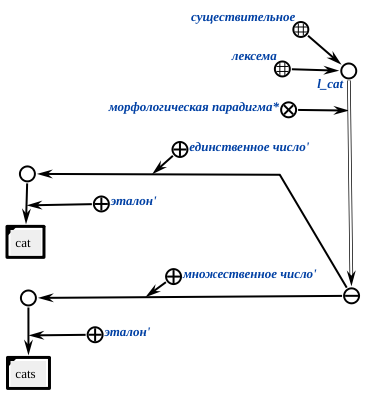
\includegraphics[width=0.4\textwidth]{images/part2/chapter_lang/lexeme_example.png}
    \caption{Пример спецификации лексемы в базе знаний.}
    \label{fig:lexeme_example}
\end{figure}

Часть речи -- категория, представляющая собой класс синтаксически эквивалентных знаков ЕЯ.

\begin{SCn}

    \scnheader{часть речи}
    \scnrelto{семейство подмножеств}{лексема}
    \scnhaselement{существительное}
    \scnhaselement{прилагательное}
    \scnhaselement{глагол}
    \scnhaselement{наречие}
    \scnhaselement{предлог}
    \scnhaselement{комплементатор}
    \scnhaselement{вспомогательный глагол}
    \scnhaselement{детерминант}

\end{SCn}

\textit{морфологическая парадигма*} - бинарное ориентированное отношение, связывающее лексему и множество ее словоформ.

Словоформа -- подмножество лексемы, которому принадлежат все вхождения лексемы с определенными грамматическими значениями. В рамках нашей онтологии словоформа понимается несколько иначе, чем принято в лингвистике, так как все вхождения лексемы в технологии OSTIS являются файлами.

При формализации синтаксиса в основном использовались стандартные положения генеративной грамматики \scncite{adger2003core}, \scncite{jackendoff1977x}, \scncite{haegeman1994introduction}, \scncite{carnie2012syntax}.

Дистрибуция знака –- это подмножество синтаксических правил, в которые входит данный знак.

Составляющая -- элемент множества C подмножеств кортежа вхождений лексем S, которое содержит в качестве элементов как сам S, так и все вхождения лексем в S, таким образом, что любые два подмножества, входящие в C, либо не пересекаются, либо одно из них включается в другое.

Непосредственно составляющая --  есть множество составляющих S, в которое входят составляющие A и B. В является непосредственно составляющей А если и только если В является подмножеством А и нет такой составляющей С, которая является подмножеством А и подмножеством которой является В.

Элементарная составляющая -- элемент кортежа вхождений лексем L, являющихся непосредственно составляющими множества составляющих C и не имеющих дочерних составляющих.

Синтаксическая группа -- класс составляющих, в который входят составляющие с вершинами, принадлежащими к одной части речи. Синтаксические группы представляют собой либо синглетон (минимально включают в себя вершину), либо упорядоченную пару, состояющую из вершины и другой синтаксической группы.

Вершина –- составляющая, дистрибуция которой совпадает с дистрибуцией всей синтаксической группы.

\begin{SCn}

    \scnheader{составляющая}
    \begin{scnrelfromset}{разбиение}
        \scnitem{синтаксическая группа}
        \scnitem{вершина}
    \end{scnrelfromset}

    \scnheader{синтаксическая группа}
% максимальная, промеж и вершины, вывести классы из примера как их пересечения
    \begin{scnrelfromset}{разбиение}
        \scnitem{именная группа}
        \begin{scnindent}
            \scntext{пояснение}{\textit{Именная группа} -- синтаксическая группа, вершиной которой является существительное.}
        \end{scnindent}
        \scnitem{глагольная группа}
        \begin{scnindent}
            \scntext{пояснение}{\textit{Глагольная группа} -- синтаксическая группа, вершиной которой является глагол.}
        \end{scnindent}
        \scnitem{группа прилагательного}
        \begin{scnindent}
            \scntext{пояснение}{\textit{Группа прилагательного} -- синтаксическая группа, вершиной которой является прилагательное.}
        \end{scnindent}
        \scnitem{наречная группа}
        \begin{scnindent}
            \scntext{пояснение}{\textit{Наречная группа} -- синтаксическая группа, вершиной которой является наречие.}
        \end{scnindent}
        \scnitem{предложная группа}
        \begin{scnindent}
            \scntext{пояснение}{\textit{Предложная группа} -- синтаксическая группа, вершиной которой является предлог.}
        \end{scnindent}
        \scnitem{группа комплементатора}
        \begin{scnindent}
            \scntext{пояснение}{\textit{Группа комплементатора} -- синтаксическая группа, вершиной которой является комплементатор.}
        \end{scnindent}
        \scnitem{временная группа}
        \begin{scnindent}
            \scntext{пояснение}{\textit{Временная группа} -- синтаксическая группа, вершиной которой является вспомогательный либо модальный глагол.}
        \end{scnindent}
        \scnitem{группа детерминанта}
        \begin{scnindent}
            \scntext{пояснение}{\textit{Группа детерминанта} -- синтаксическая группа, вершиной которой является детерминант.}
        \end{scnindent}
    \end{scnrelfromset}
    \begin{scnrelfromset}{разбиение}
        \scnitem{максимальная проекция вершины}
        \scnitem{промежуточная проекция вершины}
    \end{scnrelfromset}

\end{SCn}

При этом для упрощения могут быть введены более узкие классы, являющиеся пересечением приведенных выше, например \textit{максимальная проекция вершины группы детерминанта}.

\begin{SCn}

    \scnheader{максимальная проекция вершины группы детерминанта}
    \begin{scnreltoset}{пересечение}
        \scnitem{группа детерминанта}
        \scnitem{максимальная проекция вершины}
    \end{scnreltoset}

\end{SCn}

Пример синтаксической структуры предложения, записанный с применением введенных выше понятий представлен на рисунке~\ref{pic_tree}.

\begin{figure*}[h]
    \centering
    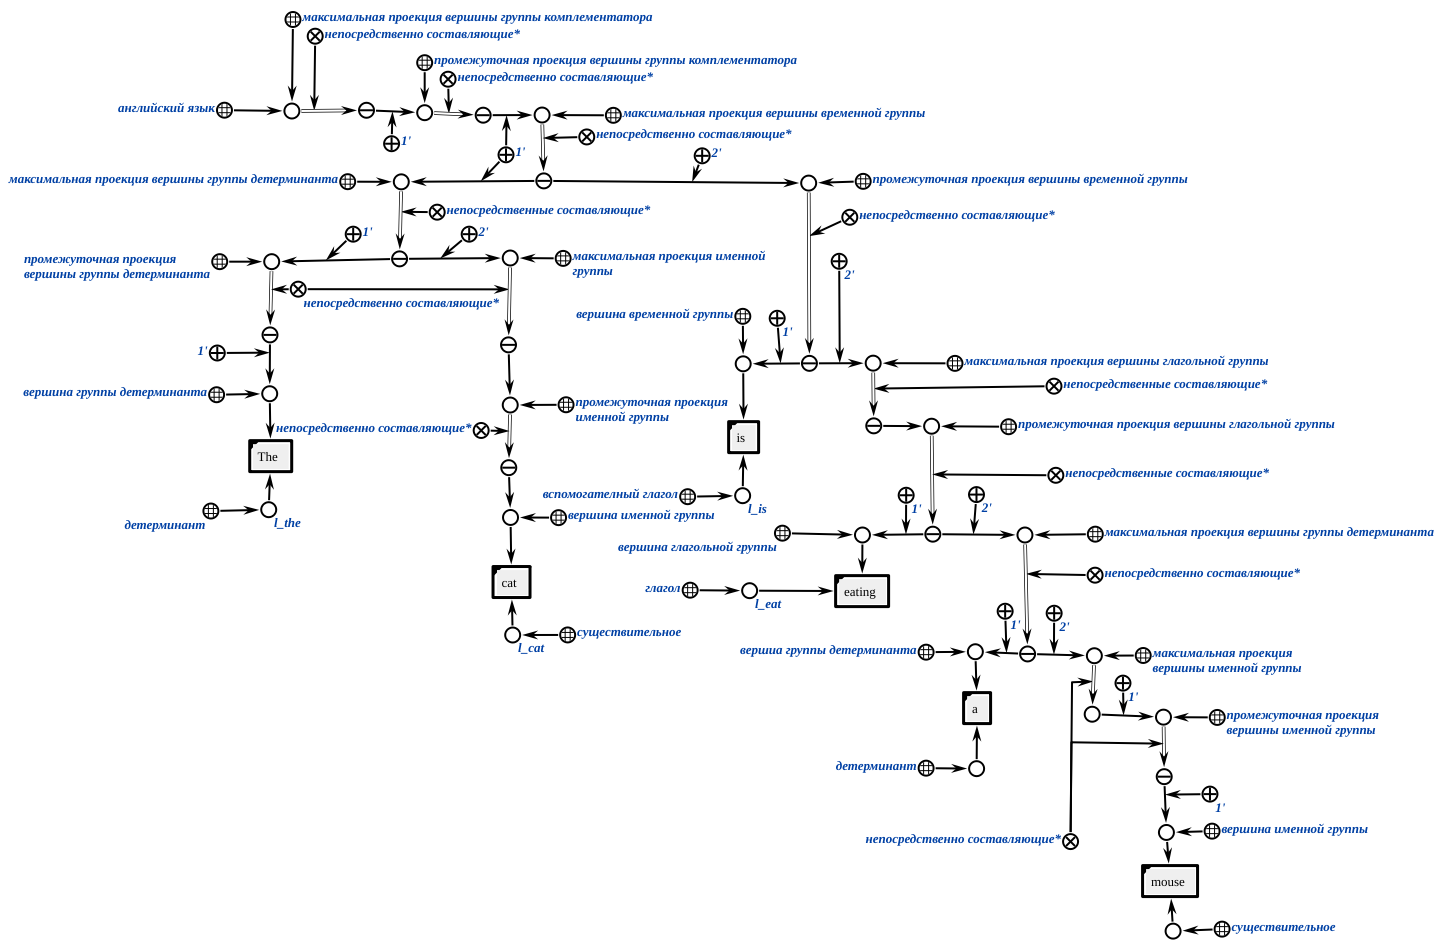
\includegraphics[width=\textwidth]{images/part2/chapter_lang/syntactic.png}
    \caption{Пример синтаксической структуры предложения.}
    \label{pic_tree}
\end{figure*}

Структуры синтаксических групп не являются произвольными -- элементы внутри группы могут граничить только с определенными множествами элементов.
Ниже приводятся возможные структуры синтаксических групп.
Знак "->"{} следует читать как "состоит из"{}.
В скобках указаны опциональные элементы.

Группа детерминанта:
\begin{textitemize}
    \item Максимальная проекция вершины группы детерминанта -> (Максимальная проекция вершины группы детерминанта) Промежуточная проекция вершины группы детерминанта
    \item Промежуточная проекция вершины группы детерминанта -> Вершина группы детерминанта (Максимальная проекция вершины именной группы)
\end{textitemize}

Именная группа:
\begin{textitemize}
    \item Максимальная проекция вершины именной группы -> (Максимальная проекция вершины группы детерминанта) Промежуточная проекция вершины именной группы
    \item Промежуточная проекция вершины именной группы -> (Максимальная проекция вершины группы прилагательного) Промежуточная проекция вершины именной группы ИЛИ Промежуточная проекция вершины именной группы (Максимальная проекция вершины предложной группы)
    \item Промежуточная проекция вершины именной группы -> Вершина именной группы (Максимальная проекция вершины предложной группы)
\end{textitemize}

Глагольная группа:
\begin{textitemize}
    \item Максимальная проекция вершины глагольной группы -> Промежуточная проекция вершины глагольной группы
    \item Промежуточная проекция вершины глагольной группы -> Промежуточная проекция вершины глагольной группы (Максимальная проекция вершины предложной группы) ИЛИ Промежуточная проекция вершины глагольной группы (Максимальная проекция вершины наречной группы)
    \item Промежуточная проекция вершины глагольной группы -> Вершина глагольной группы (Максимальная проекция вершины именной группы)
\end{textitemize}

Наречная группа:
\begin{textitemize}
    \item Максимальная проекция вершины наречной группы -> Промежуточная проекция вершины наречной группы
    \item Промежуточная проекция вершины наречной группы -> (Максимальная проекция вершины наречной группы) Промежуточная проекция вершины наречной группы
    \item Промежуточная проекция вершины наречной группы -> Вершина наречной группы (Максимальная проекция вершины предложной группы)
\end{textitemize}

Группа прилагательного:
\begin{textitemize}
    \item Максимальная проекция вершины группы прилагательного -> Промежуточная проекция вершины группы прилагательного
    \item Промежуточная проекция вершины группы прилагательного -> (Максимальная проекция вершины наречной группы) + Промежуточная проекция вершины группы прилагательного
    \item Промежуточная проекция вершины группы прилагательного -> Вершина группы прилагательного (Максимальная проекция вершины предложной группы)
\end{textitemize}

Предложная группа:
\begin{textitemize}
    \item Максимальная проекция вершины предложной группы -> Промежуточная проекция вершины предложной группы
    \item Промежуточная проекция вершины предложной группы -> Промежуточная проекция вершины предложной группы (Максимальная проекция вершины предложной группы) ИЛИ (Максимальная проекция вершины наречной группы) Промежуточная проекция вершины предложной группы
    \item Промежуточная проекция вершины предложной группы -> Вершина предложной группы (Максимальная проекция вершины именной группы)
\end{textitemize}

Временная группа:
\begin{textitemize}
    \item Максимальная проекция вершины временной группы -> (Максимальная проекция вершины группы детерминанта) Промежуточная проекция вершины временной группы
    \item Промежуточная проекция вершины временной группы -> Вершина временной группы (Максимальная проекция вершины глагольной группы)
\end{textitemize}

Группа комплементатора:
\begin{textitemize}
    \item Максимальная проекция вершины группы комплементатора -> (Максимальная проекция вершины некоторой синтаксической группы) Промежуточная проекция вершины группы комплементатора
    \item Промежуточная проекция вершины группы комплементатора -> Вершина группы комплементатора Максимальная проекция вершины временной группы
\end{textitemize}

В формальном виде данные правила можно представить следующим образом (см. рисунок~\ref{fig:pic_tree_structure_rule}).

\begin{figure*}[h]
    \centering
    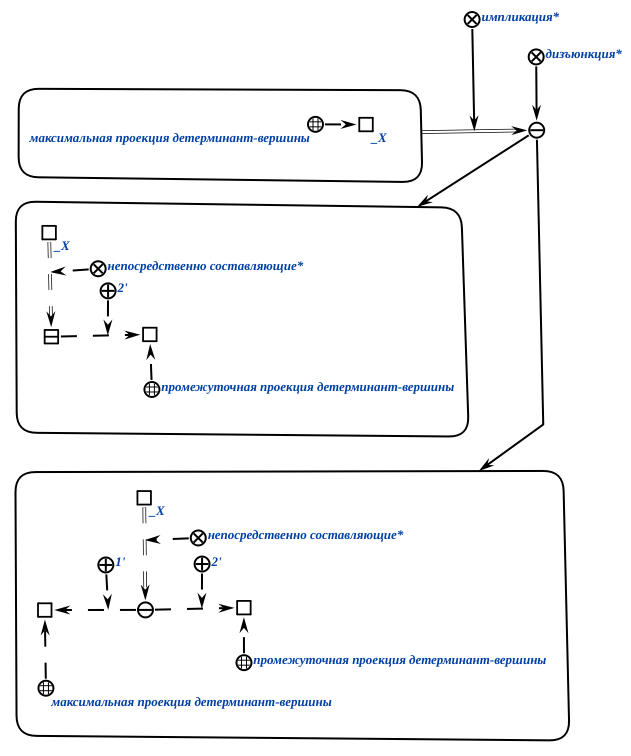
\includegraphics[width=0.8\textwidth]{images/part2/chapter_lang/tree_structure_rule.png}
    \caption{Пример правила структуры синтаксической группы.}
    \label{fig:pic_tree_structure_rule}
\end{figure*}

Комплемент -- синтаксическая группа, являющаяся сестрой вершины. Сестрами считаются составляющие, являющиеся непосредственно составляющими одной и той же составляющей.

Адъюнкт -- синтаксическая группа, являющаяся дочерью (непосредственно составляющей) промежуточной проекции и сестрой промежуточной проекции вершины той же синтаксической группы.

Спецификатор -- синтаксическая группа, являющейся дочерью максимальной проекции и сестрой промежуточной проекции.

Приведенные выше правила структуры синтаксических групп можно обобщить и свести к трем более абстрактным.

Правило спецификатора: XP -> (YP) X'

Правило адъюнкта: X' -> X' (ZP) | X' -> (ZP) X'

Правило комплемента: X' -> X (WP)

Формальное представление данных правил аналогично приведенному на рисунке~\ref{fig:pic_tree_structure_rule}.

\section{Формализация денотационной семантики естественных языков}

денотационная семантика языка специфицирует интерпретацию элементов синтаксиса данного языка и представляет собой множество формул, описывающих то, каким образом знаковым конструкциям языка ставятся в соответствие обозначаемые ими сущности и конфигурации отношений между этими сущностями.

денотационная семантика естественных языков должна обладать свойством композициональности -- т.е. интерпретация всего высказывания должна выводиться из интерпретации отдельных его частей. Таким образом, необходимо предоставить формальное описание интерпретации элементов синтаксиса ЕЯ, представленных в предыдущем разделе, а также описание правил совмещения интерпретации отдельных элементов для получения смысла всего высказывания.

В данной главе мы предлагаем вариант формализации денотационной семантики естественных языков в рамках \textit{Технологии OSTIS}, для составления которой использовались стандартные положения формальной семантики \scncite{heim1998semantics}, \scncite{Winter+2016}, \scncite{portner2008formal}.

Рассмотрим примеры правил, реализующих денотационную семантику языка. Приведенные ниже правила должны применяться последовательно и позволяют получить смысл текста естественного языка по его синтаксической структуре, "поднимаясь"{} по дереву составляющих от вершин к максимальным проекциям.

На рисунке~\textit{\nameref{fig:d_sem_1}} приведено правило, по которому происходит интерпретация вершин именной группы и группы прилагательного.
Смыслом таких вершин является класс, например: прилагательному ``черный'' соответствует множество черных объектов, а существительному ``кот'' -- множество котов.

\begin{figure}[H]
    \centering
    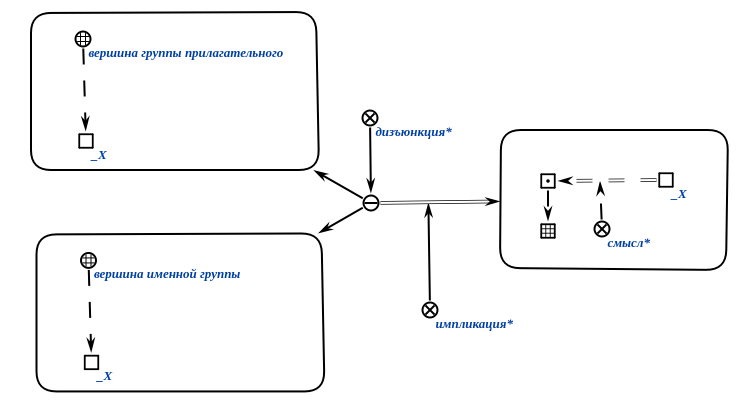
\includegraphics[width=0.8\textwidth]{images/part2/chapter_lang/d_sem_1}
    \caption{Правило интерпретации вершины группы прилагательного и вершины именной группы}
    \label{fig:d_sem_1}
\end{figure}
%в этом правиле мы интерпретируем вершины групп прилагательного и существительного - т.е. отдельные "слова"{}-прилагательные и существительные, которые у нас соответствуют классам

На рисунке~\textit{\nameref{fig:d_sem_2}} приведено правило, по которому происходит интерпретация именной группы, максимальная проекция которой включается в себя также группу прилагательного.
Как говорилось выше, для применения данного правила необходимо предварительное применение правила, представленного на рисунке~\textit{\nameref{fig:d_sem_1}}.
Смыслом таких конструкций является класс, являющийся результатом пересечения классов, полученных в результате интерпретации вершин групп прилагательного и именной группы по отдельности. Например: ``черный кот''{} -- множество черных котов, пересечение множества котов и черных объектов. %ну все, теперь включаю мою кошку в соавторы

\begin{figure*}[h]
    \centering
    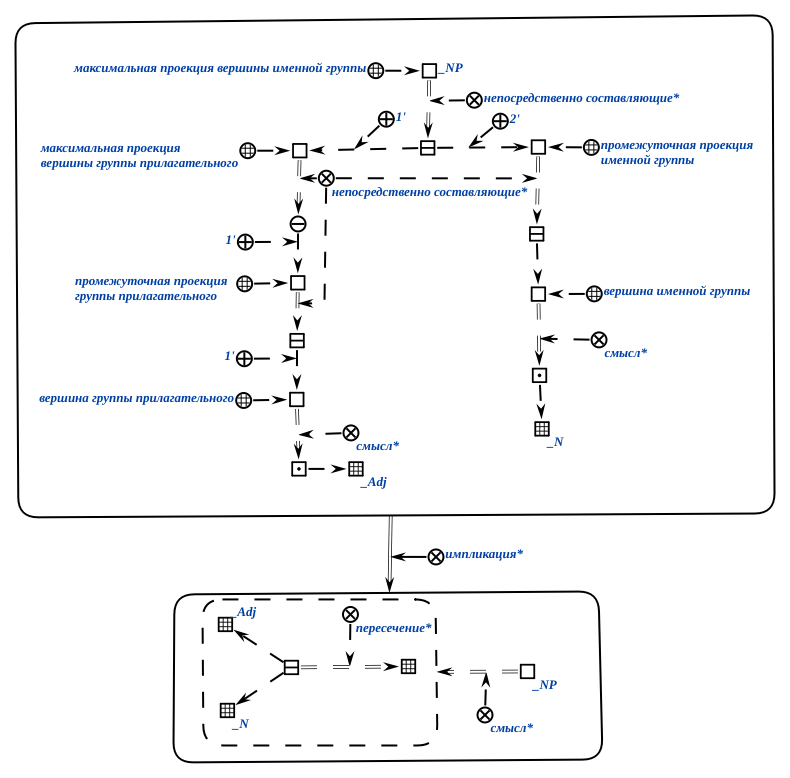
\includegraphics[width=0.8\textwidth]{images/part2/chapter_lang/d_sem_2.png}
    \caption{Правило интерпретации максимальной проекции вершины именной группы}
    \label{fig:d_sem_2}
\end{figure*}
%тут мы комбинируем смыслы прилагательного и существительного, которые входят в одну именную группу

На рисунке~\textit{\nameref{fig:d_sem_3}} приведено правило, по которому происходит интерпретация глагольной группы. Необходимость включения в посылку правила всей ветки глагольной группы объясняется ее необходимостью для определения типа глагола -- данное правило предназначено для интерпретации непереходных глаголов. Смыслом такой конструкции является класс действий.

\begin{figure*}[h]
    \centering
    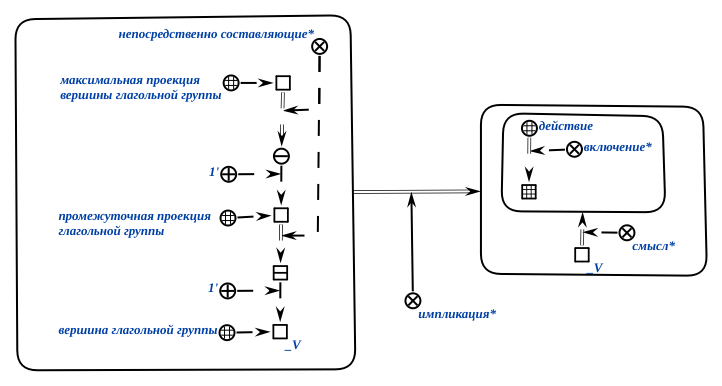
\includegraphics[width=0.8\textwidth]{images/part2/chapter_lang/d_sem_3.png}
    \caption{Правило интерпретации максимальной проекции вершины глагольной группы, содержащей непереходный глагол}
    \label{fig:d_sem_3}
\end{figure*}
%тут мы задаем интерпретацию всей глагольной группы (макс проекции) только для непереходных глаголов. написать, что смотрим по всей структуре группы целиком, потому что для того, чтобы отличить непереходный от переходного нам нужна вся ветка глагольной группы в дереве целиком

На рисунке~\textit{\nameref{d_sem_4}} приведено правило, по которому происходит интерпретация группы детерминанта с неопределенным артиклем. Смыслом такой конструкции является существование элемента класса, являющегося смыслом входящей в состав данной группы детерминанта именной группы.

\begin{figure*}[h]
    \centering
    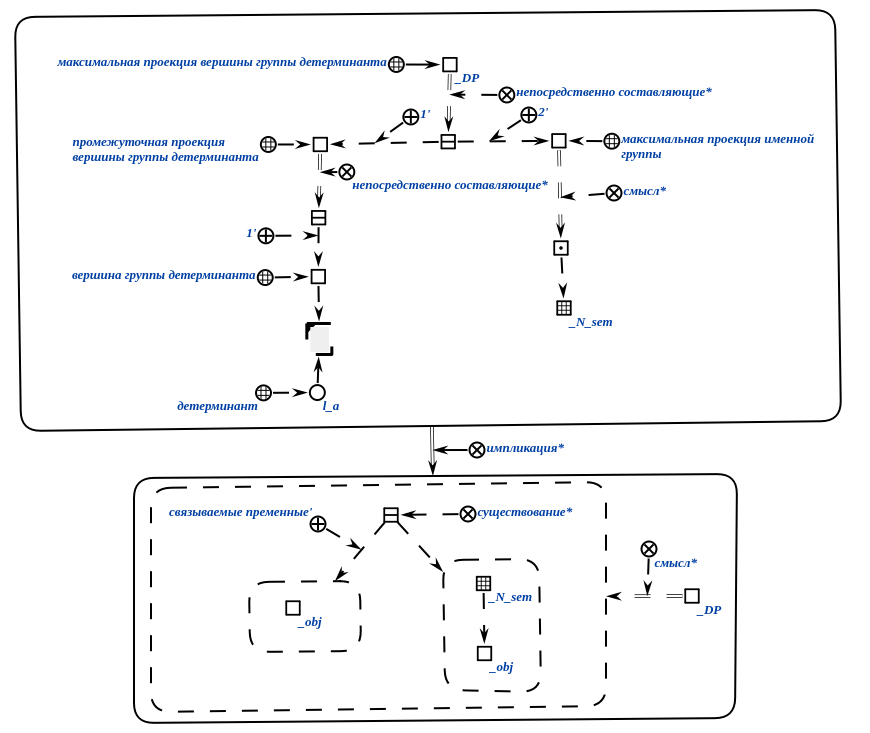
\includegraphics[width=0.8\textwidth]{images/part2/chapter_lang/d_sem_4.png}
    \caption{Правило интерпретации максимальной проекции вершины группы детерминанта}
    \label{d_sem_4}
\end{figure*}
%тут задается интерпретация сочетания именной группы с артиклем (в данном случае неопределенным)

На рисунке~\textit{\nameref{fig:d_sem_5}} приведено правило, по которому происходит интерпретация промежуточной проекции вершины временной группы, состоящей из вспомогательного глагола и полнозначного глагола. Вспомогательный глагол в данном случае задет класс действий по времени (является ли оно запланированным, выполняемым, уже выполненным и т.д.).

\begin{figure*}[h]
    \centering
    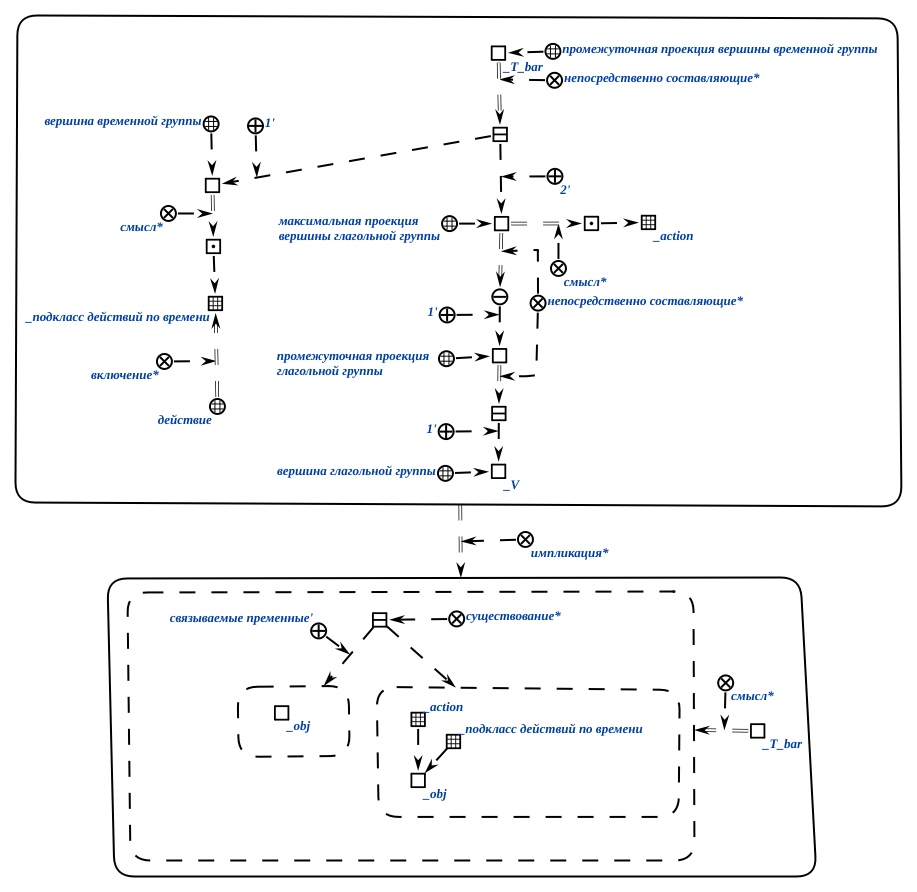
\includegraphics[width=0.8\textwidth]{images/part2/chapter_lang/d_sem_5.png}
    \caption{Правило интерпретации промежуточной проекции вершины временной группы}
    \label{fig:d_sem_5}
\end{figure*}
%тут задаем интерпретацию сочетания вспомогательного глагола и основного глагола. вспомогательный у нас соответствует классу действий по времени

На рисунке~\textit{\nameref{fig:d_sem_6}} приведено правило, по которому происходит интерпретация максимальной проекции вершины временной группы на основе полученного на предыдущем шаге смысла промежуточной проекции вершины временной группы и смысла максимальной проекции группы детерминанта.

\begin{figure*}[h]
    \centering
    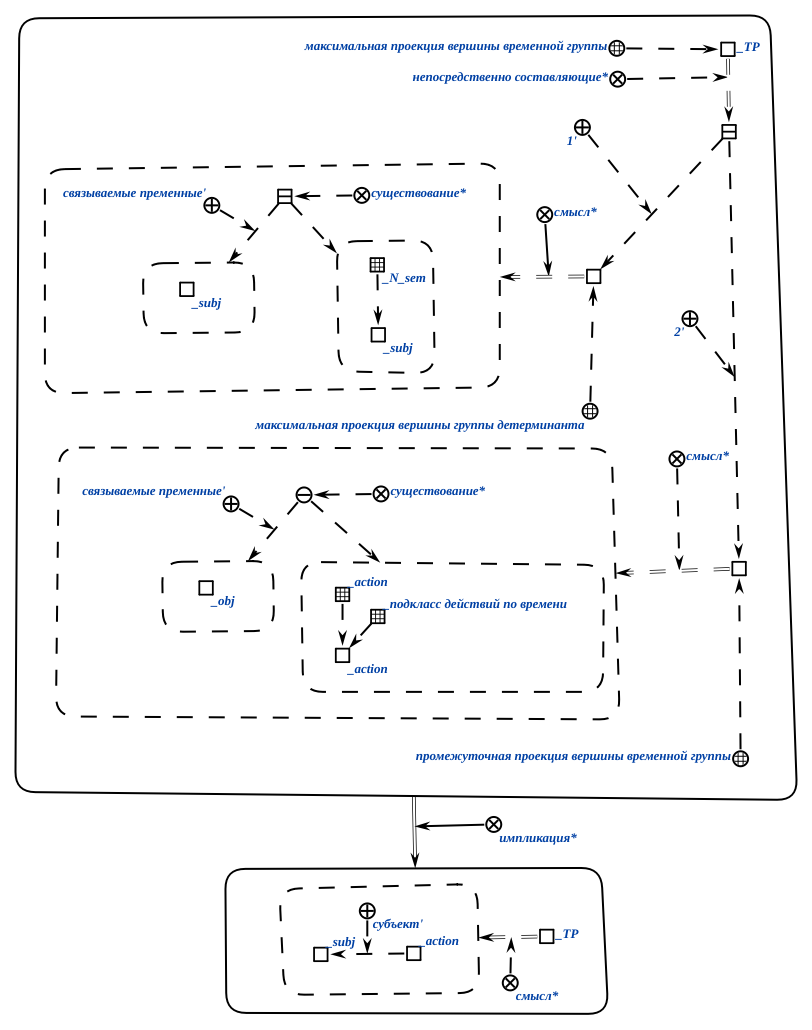
\includegraphics[width=0.8\textwidth]{images/part2/chapter_lang/d_sem_6.png}
    \caption{Правило интерпретации максимальной проекции вершины временной группы}
    \label{fig:d_sem_6}
\end{figure*}
%тут задаем интерпретацию для аргументной структуры непереходного глагола (сочетания подлежащего с непереходным глаголом)

На рисунке~\textit{\nameref{fig:d_sem_7}} приведено правило, по которому происходит интерпретация максимальной проекции вершины группы комплементатора на основе полученных на предыдущих шагах смыслов более частных конструкций. Данным правилом задается интерпретация предложения с переходным глаголом.

\begin{figure*}[h]
    \centering
    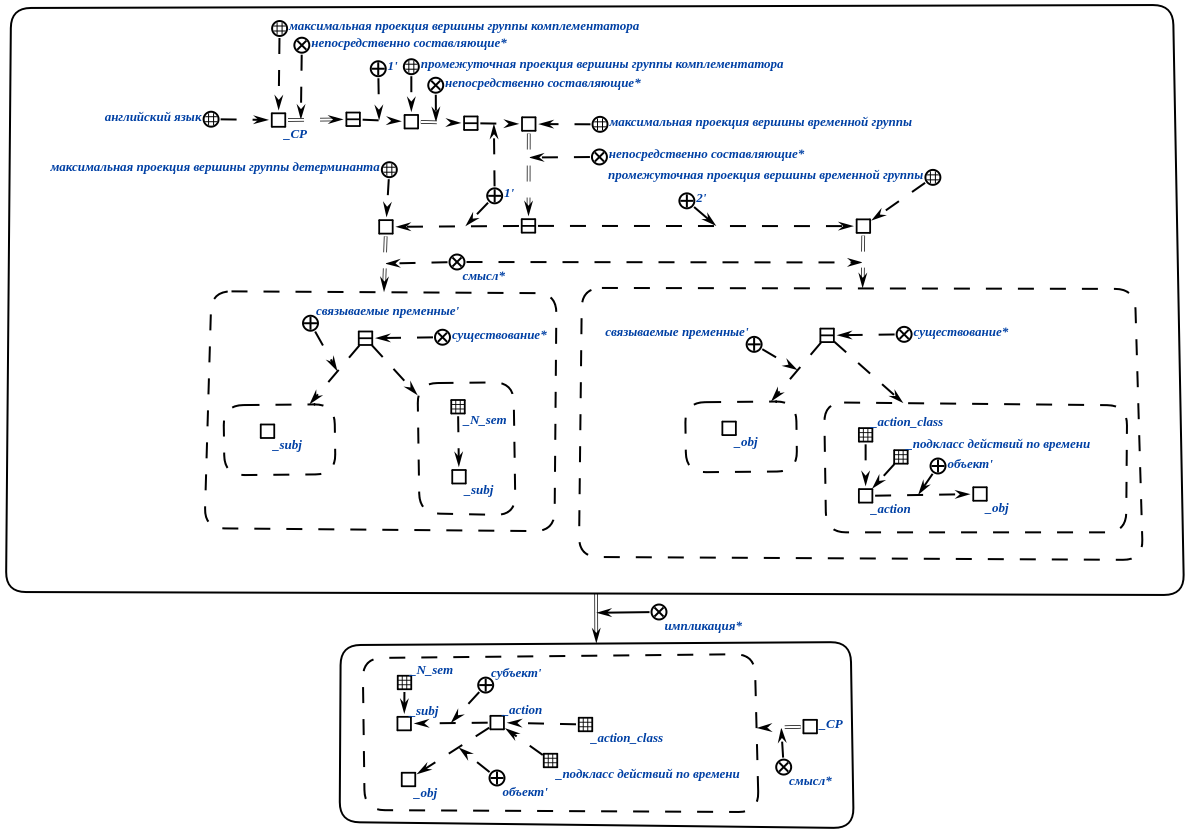
\includegraphics[width=0.8\textwidth]{images/part2/chapter_lang/d_sem_7.png}
    \caption{Правило интерпретации предложения с переходным глаголом}
    \label{fig:d_sem_7}
\end{figure*}
%тут задаем интерпретацию аргументной структуры переходного глагола (сочетания переходного глагола с его аргументами - подлажещим и дополнением)

%\input{author/references}

\begin{partbacktext}
\part{Многоагентные модели решателей задач интеллектуальных компьютерных систем нового поколения}
\noindent Описание к главе
\end{partbacktext}

\chapter{Формализация понятий действия, задачи, метода, средства, навыка и технологии}
\chapauthortoc{Шункевич Д.В.\\Ковалёв М.В.}
\label{chapter_actions}

\vspace{-7\baselineskip}

\begin{SCn}
	\begin{scnrelfromlist}{автор}
		\scnitem{Шункевич Д.В.}
		\scnitem{Ковалёв М.В.}
	\end{scnrelfromlist}

	\bigskip

	\scntext{аннотация}{В главе уточнена формальная трактовка таких понятий, как \textit{действие}, \textit{задача}, \textit{класс действий}, \textit{класс задач}, \textit{метод}, \textit{навык}, что в совокупности позволило определить на их основе понятие \textit{модели решения задач}. Также уточнены понятия \textit{деятельности}, \textit{вида деятельности} и \textit{технологии}.}

	\bigskip

	\begin{scnrelfromlist}{подраздел}
		\scnitem{\ref{sec_action_concept}~\nameref{sec_action_concept}}
		\scnitem{\ref{sec_problem_concept}~\nameref{sec_problem_concept}}
		\scnitem{\ref{sec_action_and_problem_classes}~\nameref{sec_action_and_problem_classes}}
		\scnitem{\ref{sec_method_concept}~\nameref{sec_method_concept}}
		\scnitem{\ref{sec_skill_concept}~\nameref{sec_skill_concept}}
		\scnitem{\ref{sec_method_lang_concept}~\nameref{sec_method_lang_concept}}
		\scnitem{\ref{sec_problem_solving_model}~\nameref{sec_problem_solving_model}}
		\scnitem{\ref{sec_activity_and_technology}~\nameref{sec_activity_and_technology}}
	\end{scnrelfromlist}

	\bigskip

	\begin{scnrelfromlist}{ключевое понятие}
		\scnitem{воздействие}
		\scnitem{действие}
		\scnitem{задача}
		\scnitem{класс действий}
		\scnitem{класс задач}
		\scnitem{метод}
		\scnitem{язык представления методов}
		\scnitem{модель решения задач}
		\scnitem{навык}
		\scnitem{деятельность}
		\scnitem{вид деятельности}
		\scnitem{технология}
	\end{scnrelfromlist}

	\bigskip

	\begin{scnrelfromlist}{библиографическая ссылка}
		\scnitem{\scncite{Shunkevich2021}}
		\scnitem{\scncite{Standart2021}}
		\scnitem{\scncite{Fayans2020}}
		\scnitem{\scncite{Pospelov1986}}
		\scnitem{\scncite{Shunkevich2018}}
	\end{scnrelfromlist}

\end{SCn}

\section*{Введение в Главу \ref{chapter_actions}}
Возможности решателя задач интеллектуальной системы в значительной степени определяются качеством ее базы знаний. Другими словами, при разработке решателей задач необходимо описывать не только \textit{операционную семантику} решателя, то есть семейство интерпретаторов соответствующих моделей решения задач, но и \textit{декларативную семантику} модели решения задач, то есть собственно тексты программ (не программ низкоуровневых агентов, а программ более высокого уровня, интерпретируемых соответствующим набором агентов), логические утверждения, конкретные конфигурации искусственных нейронных сетей и так далее.

В рамках данной главы формально уточняются в рамках соответствующего набора онтологий такие понятия, как \textit{действие}, \textit{задача}, \textit{модель решения задач}, \textit{метод}, \textit{навык} и другие, на основе которых в \textit{Главе \ref{chapter_situation_management} \nameref{chapter_situation_management}} уточняется собственно модель гибридного \textit{решателя задач ostis-системы}.

%TODO Уточнить, будет ли где-то ранее говориться про sc-агенты и многоагентный подход
Разработка указанного семейства онтологий позволяет:
\begin{textitemize}
	\item явно связать \textit{класс задач} и способ (метод) решения задач данного класса;
	\item это, в свою очередь, позволит накапливать более сложные компоненты решателей задач и еще больше упростить их интеграцию, поскольку вместе с коллективом sc-агентов в соответствующий компонент также будут входить необходимые фрагменты базы знаний, априори согласованные с указанным коллективом sc-агентов;
	\item это, в свою очередь, позволит сделать средства автоматизации разработки решателей задач более интеллектуальными, в частности, позволит автоматизировать процесс подбора компонентов решателя на основе спецификации классов задач, которые должна уметь решать проектируемая интеллектуальная система;
	\item в дальнейшем это позволит интеллектуальной системе самостоятельно обращаться в библиотеку компонентов решателей задач (см. \ref{sec_ps_components}~\nameref{sec_ps_components}) и подбирать компоненты, исходя из новых классов задач, с которыми столкнулась система, то есть позволит интеллектуальной системе самостоятельно изучать новые \textit{навыки};
	\item с другой стороны, такой подход позволит интеллектуальной системе самостоятельно подобрать комбинацию моделей решения задач для решения задач определенного класса (точнее говоря, поскольку в основу решателя положен многоагентный подход, то коллектив sc-агентов, интерпретирующих различные модели решения задач, сможет лучше определить, какие именно из sc-агентов и в каком порядке должны работать при решении конкретной комплексной задачи).
\end{textitemize}

Результаты, ранее полученные авторами в данной области исследований опубликованы в таких работах, как \scncite{Shunkevich2021}, \scncite{Standart2021}.

\section{Понятие действия}
\label{sec_action_concept}

\begin{SCn}
	\begin{scnrelfromlist}{ключевое понятие}
		\scnitem{воздействие}
		\scnitem{действие}
		\scnitem{субъект}
		\scnitem{информационное действие}
		\scnitem{поведенческое действие}
		\scnitem{эффекторное действие}
		\scnitem{рецепторное действие}
		\scnitem{атомарное действие}
		\scnitem{неатомарное действие}
	\end{scnrelfromlist}

	\begin{scnrelfromlist}{ключевое отношение}
		\scnitem{субъект\scnrolesign}
		\scnitem{объект\scnrolesign}
		\scnitem{цель*}
	\end{scnrelfromlist}
\end{SCn}

Прежде чем говорить о моделях решения задач и решателя задач, необходимо формально уточнить понятие задачи и понятие действия, направленного на решение той или иной задачи или ее подзадач.

В рамках \textit{Технологии OSTIS} задачу будем трактовать как формальную спецификацию некоторого действия, поэтому целесообразно вначале уточнить понятие \textbf{\textit{действия}}, которое определяется через понятие \textbf{\textit{воздействия}}. Рассмотрим спецификацию понятия \textit{воздействие} в SCn-коде.

\begin{SCn}
	\scnheader{воздействие}
	\scnidtf{\textit{процесс} воздействия одной сущности (или некоторого множества \textit{сущностей}) на другую \textit{сущность} (или на некоторое множество других \textit{сущностей})}
	\scnidtf{\textit{процесс}, в котором могут быть явно выделены хотя бы одна воздействующая сущность (\textit{субъект\scnrolesign}) и хотя бы одна \textit{сущность}, на которую осуществляется воздействие (\textit{объект\scnrolesign})}
	\scnidtf{акция}
	\scnsubset{процесс}
	\begin{scnindent}
		\scnidtf{динамическая структура}
	\end{scnindent}

	\scnheader{субъект}
	\scnidtf{активная сущность}
	\scnsubset{сущность}
	\scnidtftext{часто используемый sc-идентификатор}{индивид}

	\scnheader{субъект\scnrolesign}
	\scnidtf{воздействующая сущность\scnrolesign}
	\scnidtf{сущность, создающая \textit{причину} изменений другой сущности (объекта)\scnrolesign}

	\scnheader{объект\scnrolesign}
	\scnidtf{воздействуемая сущность\scnrolesign}
	\scnidtf{сущность, являющаяся в рамках заданного воздействия исходным условием (аргументом), необходимым для выполнения этого воздействия\scnrolesign}
\end{SCn}

Каждому \textit{воздействию} может быть поставлен в соответствие (1) некоторый \textit{субъект\scnrolesign}, то есть сущность, осуществляющая \textit{воздействие} (в частности, это может быть некоторое физическое поле), и (2) некоторый \textit{объект\scnrolesign}, то есть сущность, на которую воздействие направлено. Если \textit{воздействие} связано с \textit{материальной сущностью}, то его объектом является либо сама эта \textit{материальная сущность}, либо некоторая ее пространственная часть.

Поскольку \textit{воздействия} являются частным видом \textit{процессов}, воздействиями наследуются все свойства \textit{процессов}. В частности, используются все \textit{параметры}, заданные на множестве \textit{процессов}, например, \textit{длительность*}, \textit{момент начала процесса*}, \textit{момент завершения процесса\scnsupergroupsign}. Подробнее эти отношения описываются в \textit{Главе \ref{chapter_top_ontologies} \nameref{chapter_top_ontologies}}.

Также, так как воздействие является процессом и, соответственно, представляет собой \textit{динамическую структуру}, то и знак \textit{субъекта воздействия\scnrolesign}, и знак \textit{объекта воздействия\scnrolesign} являются элементами данной структуры. В связи с этим можно рассматривать отношения \textit{субъект воздействия\scnrolesign} и \textit{объект воздействия\scnrolesign} как \textit{ролевые отношения}. Данный факт не запрещает вводить аналогичные \textit{неролевые отношения}, однако это нецелесообразно.

Рассмотрим спецификацию понятия \textit{действие} в SCn-коде.
\begin{SCn}
	\scnheader{действие}
	\scnidtf{\textit{воздействие}, в котором \textit{субъект\scnrolesign} осуществляет \textit{воздействие} целенаправленно, то есть в соответствии с некоторой \textit{целью*}}
	\scnidtf{целенаправленное воздействие, выполняемое одним или несколькими субъектами (кибернетическими системами) с возможным применением некоторых инструментов}
	\scnidtf{акт}
	\scnidtf{операция}
	\scnidtf{осознанное воздействие}
	\scnidtf{активное воздействие}
	\scnsubset{воздействие}
	\begin{scnindent}
		\scnidtf{процесс, в котором могут быть явно выделены хотя бы одна воздействующая сущность (субъект воздействия\scnrolesign) и хотя бы одна сущность, на которую осуществляется воздействие (объект воздействия\scnrolesign)}
		\scnsubset{процесс}
	\end{scnindent}

	\scnidtf{целенаправленный (\scnqq{осознанный}) процесс, выполняемый (управляемый, реализуемый) неким субъектом}
	\scnidtf{работа}
	\scnidtf{процесс решения некоторой задачи}
	\scnidtf{процесс достижения некоторой цели}
	\scnidtf{целостный фрагмент некоторой деятельности}
	\scnidtf{целенаправленный процесс, управляемый некоторым субъектом}
	\scnidtf{процесс выполнения некоторого действия некоторым субъектом (исполнителем) над некоторыми объектами}

	\scnheader{цель*}
	\scnidtf{целевая ситуация*}
	\scnsubset{спецификация*}
	\scnidtf{описание того, что требуется получить (какая ситуация должна быть достигнута) в результате выполнения заданного (специфицируемого) действия*}
\end{SCn}

Каждое \textit{действие}, выполняемое тем или иным \textit{субъектом}, трактуется как процесс решения некоторой задачи, то есть процесс достижения заданной \textit{цели*} в заданных условиях, и, следовательно, выполняется целеноправленно. При этом явное указание \textit{действия} и его связи с конкретной задачей может не всегда присутствовать в памяти. Некоторые \textit{задачи} могут решаться определенными субъектами перманентно, например, оптимизация \textit{базы знаний}, поиск некорректностей и так далее и для подобных задач не всегда есть необходимость явно вводить \textit{структуру}, являющуюся формулировкой \textit{задачи}.

Каждое \textit{действие} может обозначать сколь угодно малое преобразование, осуществляемое во внешней среде либо в памяти некоторой \textit{кибернетической системы}, однако в памяти явно вводятся знаки только тех \textit{действий}, для которых есть небходимость явно хранить в памяти их спецификацию в течение некоторого времени.

При выполнении \textit{действия} можно выделить этапы:
\begin{scnitemize}
	\item построение \textit{плана действия}, декомпозиция (детализация) действия в виде системы его \textit{поддействий};
	\item выполнение построенного плана \textit{действия}.
\end{scnitemize}

Класс действий имеет разбиение по следующим признакам:
\begin{scnitemize}
	\item место выполнения действия;
	\item функциональная сложность действия;
	\item многоагентность выполнения действия;
	\item текущее состояние действия.
\end{scnitemize}

Далее рассмотрим разбиение по каждому признаку.

\begin{SCn}
	\scnheader{действие}
	\scnrelfrom{разбиение}{Типология классов действий по признаку места выполнения действия}
	\begin{scnindent}
		\begin{scneqtoset}
			\scnitem{информационное действие}
			\begin{scnindent}
				\scnidtf{действие, выполняемое в памяти субъекта действия}
				\scnidtf{действие, выполняемое в памяти}
				\scnidtf{действие кибернетической системы, направленное на обработку информации, хранимой в её памяти}
			\end{scnindent}
			\scnitem{поведенческое действие}
			\begin{scnindent}
				\scnidtf{действие, выполняемое во внешней среде субъекта действия}
			\end{scnindent}
			\scnitem{рецепторное действие}
			\begin{scnindent}
				\scnidtf{сенсорное действие}
			\end{scnindent}
			\scnitem{эффекторное действие}
		\end{scneqtoset}
	\end{scnindent}
\end{SCn}

Результатом выполнения \textbf{\textit{информационного действия}} в общем случае является некоторое новое состояние памяти информационной системы (не обязательно \textit{sc-памяти}), достигнутое исключительно путем преобразования информации, хранящейся в памяти системы, то есть либо посредством генерации новых знаний на основе уже имеющихся, либо посредством удаления знаний, по каким-либо причинам ставших ненужными. Следует отметить, что если речь идет об изменении состояния \textit{sc-памяти}, то любое преобразование информации можно свести к ряду атомарных действий по генерации, удалению или изменению инцидентности \textit{sc-элементов} относительно друг друга.

В случае \textbf{\textit{поведенческого действия}} результатом его выполнения будет новое состояние внешней среды. Очень важно отметить, что под внешней средой в данном случае понимаются также и компоненты системы, внешние с точки зрения памяти, то есть не являющиеся хранимыми в ней информационными конструкциями. К таким компонентам можно отнести, например, различные манипуляторы и прочие средства воздействия системы на внешний мир, то есть к поведенческим задачам можно отнести изменение состояния механической конечности робота или непосредственно вывод некоторой информации на экран для восприятия пользователем.

Каждое \textbf{\textit{рецепторное действие}} обозначает класс \textit{действий}, которые осуществляют преобразования в памяти субъекта действия под воздействием внешней среды.

Соответственно, каждое \textbf{\textit{эффекторное действие}} обозначает класс \textit{действий}, которые осуществляют преобразования внешней среды под воздействием памяти субъекта воздействия.

Также действия могут разбиваться по признаку их функциональной сложности.
\begin{SCn}
	\scnheader{действие}
	\scnrelfrom{разбиение}{Типология классов действий по признаку функциональной сложности действия}
	\begin{scnindent}
		\begin{scneqtoset}
			\scnitem{атомарное действие}
			\begin{scnindent}
				\scnidtf{элементарное действие}
			\end{scnindent}
			\scnitem{неатомарное действие}
			\begin{scnindent}
				\scnidtf{неэлементарное действие}
				\scnidtf{неатомарное действие}
				\begin{scnrelfromset}{покрытие}
					\scnitem{легко выполнимое неатомарное действие}
					\scnitem{трудно выполнимое неатомарное действие}
					\begin{scnindent}
						\scnidtf{интеллектуальное действие}
					\end{scnindent}
				\end{scnrelfromset}
			\end{scnindent}
		\end{scneqtoset}
	\end{scnindent}
\end{SCn}

Разберем подробнее каждый элемент приведенной иерархии.
\textbf{\textit{атомарное действие}}  выполняется одним индивидуальным субъектом и не включает в себя выполнение каких-либо дочерних действий.

Соответственно, \textbf{\textit{неатомарное действие}} является действием, выполнение которого требует декомпозиции этого действия на множество его \uline{поддействий}, то есть частных действий более низкого уровня. Более частные действия могут выполняться как последовательно, так и параллельно.

Декомпозиция неатомарного действия на поддействия может иметь весьма сложный иерархический вид с большим числом уровней иерархии, то есть поддействиями \textit{неатомарного действия} могут быть также \textit{неатомарные действия}. Уровень сложности действия можно определять (1) общим числом его поддействий и (2) числом уровней иерархии этих поддействий. Примером может служить запись одной и той же процедурной программы на языке программирования более высокого уровня и на языке программирования более низкого уровня. В данном случае атомарность действий строго определяется на уровне языка.

Темпоральные соотношения между \textit{поддействиями} неатомарного \textit{действия} могут быть самые различные, но в пройстейшем случае \textit{неатомарное действие} представляет собой строгую последовательность \textit{действий} более низкого уровня иерархии.

В состав \textit{неатомарного действия} могут входить не только \textit{собственно поддействия} этого \textit{неатомарного действия}, но также и специальные \textit{поддействия}, осуществляющие \uline{управление} процессом выполнения \textit{неатомарного действия}, и, в частности, \textit{поддействия}, осуществляющие инициирование поддействий, передачу управления \textit{поддействиям}.

Действие можно назвать \textbf{\textit{легко выполнимым неатомарным действием}} в случае, когда для выполнения этого действия известен соответствующий \textit{метод} и соответствующие этому методу исходные данные, а также (для действий, выполняемых во внешней среде) имеются в наличии все необходимые исходные объекты (расходные материалы и комплектация), а также средства (инструменты).

В свою очередь, \textbf{\textit{трудно выполнимым неатомарным действием}} действие является тогда, когда для его выполнения в текущий момент либо неизвестен соответствующий \textit{метод}, либо возможные \textit{методы} известны, но отсутствуют условия их применения. Это действие декомпозируется на несколько самостоятельных поддействий, каждое из которых выявляет (локализует) противоречия (ошибки) конкретного формализуемого вида, для которого в базе знаний существует точное определение.

Признак многоагентности выполнения действия характеризует количество субъектов, выполнеяющих действие.
\begin{SCn}
	\scnheader{действие}
	\scnrelfrom{разбиение}{Типология классов действий по признаку многоагентности выполнения действия}
	\begin{scnindent}
		\begin{scneqtoset}
			\scnitem{индивидуальное действие}
			\begin{scnindent}
				\scnidtf{действие, выполняемое одним субъектом (агентом)}
				\scnidtf{действие, выполняемое индивидуальной кибернетической системой}
			\end{scnindent}
			\scnitem{коллективное действие}
			\begin{scnindent}
				\scnidtf{действие, выполняемое коллективом субъектов (многоагентной системой)}
				\scnidtf{действие, выполняемое коллективом кибернетических систем (коллективом субъектов)}
				\scnsuperset{действие, выполняемое коллективом людей}
				\scnsuperset{действие, выполняемое коллективом индивидуальных компьютерных систем}
				\scnsuperset{действие, выполняемое коллективом людей и индивидуальных компьютерных систем}
				\begin{scnindent}
					\scnsuperset{действие, выполняемое Экосистемой OSTIS}
					\scnsuperset{действие, выполняемое одним человеком во взаимодействии с одной индивидуальной компьютерной системой}
				\end{scnindent}
			\end{scnindent}
		\end{scneqtoset}
	\end{scnindent}
\end{SCn}

Последним признаком разбиения классов действия является признак текущего состояния действия.
\begin{SCn}
	\scnheader{действие}
	\scnrelfrom{разбиение}{Типология классов действий по признаку текущего состояния действия}
	\begin{scnindent}
		\begin{scneqtoset}
			\scnitem{планируемое действие}
			\begin{scnindent}
				\scnidtf{запланированное, но не инициированное действие}
				\scnidtf{будущее действие}
			\end{scnindent}
			\scnitem{инициированное действие}
			\begin{scnindent}
				\scnidtf{действие, ожидающее начала своего выполнения}
				\scnidtf{действие, подлежащее выполнению}
			\end{scnindent}
			\scnitem{выполняемое действие}
			\begin{scnindent}
				\scnidtf{активное действие}
				\scnidtf{действие, выполняемое в текущий момент}
				\scnidtf{настоящее действие}
			\end{scnindent}
			\scnitem{прерванное действие}
			\begin{scnindent}
				\scnidtf{действие, ожидающее продолжения своего выполнения}
				\scnidtf{отложенное действие}
			\end{scnindent}
			\scnitem{выполненное действие}
			\begin{scnindent}
				\scnidtf{завершенное действие}
				\scnidtf{прошлое действие}
				\begin{scnsubdividing}
					\scnitem{успешно выполненное действие}
					\scnitem{безуспешно выполненное действие}
					\begin{scnindent}
						\scnsuperset{действие, выполненное с ошибкой}
					\end{scnindent}
				\end{scnsubdividing}
			\end{scnindent}
			\scnitem{отмененное действие}
		\end{scneqtoset}
	\end{scnindent}
\end{SCn}

Во множество \textbf{\textit{планируемых действий}} входят \textit{действия}, начало выполнение которых запланировано на какой-либо момент в будущем(\textit{начало*}).

Во множество \textbf{\textit{инициированных действий}} входят \textit{действия}, выполнение которых инициировано в результате какого-либо события.
В общем случае, \textit{действия} могут быть инициированы по следующим причинам:
\begin{scnitemize}
	\item явно путем проведения соответствующей \textit{sc-дуги принадлежности} каким-либо \textit{субъектом (заказчиком*)}. В случае действия в \textit{sc-памяти}, оно может быть инициировано как внутренним \textit{sc-агентом} системы, так и пользователем при помощи соответствующего пользовательского интерфейса. При этом, спецификация действия может быть сформирована одним \textit{sc-агентом}, а собственно добавление во множество \textit{инициированных действий} может быть осуществлено позже другим \textit{sc-агентом};
	\item в результате того, что одно или несколько \textit{действий}, предшествовавших данному в рамках некоторой декомпозиции, стали \textit{прошлыми сущностями} (процедурный подход);
	\item в результате того, что в \textit{памяти} системы появилась конструкция, соответствующая некоторому условию инициирования \textit{sc-агента}, который должен выполнить данное \textit{действие} (декларативный подход).
\end{scnitemize}

Следует отметить, что декларативный и процедурный подходы можно рассматривать как две крайности, использование только одной из которых не является удобным и целесообразным. При этом, например, принципы инициирования по процедурному подходу могут быть полностью сведены к набору декларативных условий инициирования, но как было сказано, это не всегда удобно и наиболее рациональным будет комбинировать оба подхода в зависимости от ситуации.

Принадлежность некоторого \textit{действия} множеству \textit{инициированных действий} говорит о том, что, по мнению некоторого \textit{субъекта} (заказчика, инициатора), оно готово к выполнению и должно быть выполнено, то есть спецификация данного \textit{действия} по мнению данного \textit{субъекта} сформирована в степени, достаточной для решения поставленной \textit{задачи} и существует некоторый другой \textit{субъект} (исполнитель), который может приступать к выполнению \textit{действия}. Однако стоит отметить, что с точки зрения \textit{исполнителя} такая спецификация \textit{действия} в общем случае может оказаться недостаточной или некорректной.

Во множество \textbf{\textit{выполняемых действий}} входят \textit{действия}, к выполнению которых приступил какой-либо из соответствующих \textit{субъектов}.
Попадание \textit{действия} в данное множество говорит о следующем:
\begin{scnitemize}
	\item рассматриваемое \textit{действие} уже попало во множество \textit{инициированных действий};
	\item существует как минимум один \textit{субъект}, условие инициирования которого соответствует спецификации данного \textit{действия}.
\end{scnitemize}

После того, как собственно процесс выполнения завершился, \textit{действие} должно быть удалено из множества \textit{выполняемых действий} и добавлено во множество \textit{выполненных действий} или какое-либо из его подмножеств.

Понятие \textit{выполняемое действие} является неосновным, и вместо того, чтобы относить конкретные действия к данному классу, их относят к классу \textit{настоящих сущностей}.

Во множество \textbf{\textit{прерванных действий}} входят \textit{действия}, которые уже были инициированы, однако их выполнение невозможно по каким-либо причинам, например в случае, когда у исполнителя в данный момент есть более приоритетные задачи.

Во множество \textbf{\textit{выполненных действий}} попадают \textit{действия}, выполнение которых завершено с \uline{точки зрения \textit{субъекта}}, осуществлявшего их выполнение. Таким образом, понятие \textit{выполненного действия} является относительным, поскольку с точки зрения разных субъектов одно и то же действие может считаться выполненным или все еще выполняющимся.

В зависимости от результатов конкретного процесса выполнения, рассматриваемое \textit{действие} может стать элементом одного из подмножеств множества \textit{выполненных действий}.

Понятие \textit{выполненное действие} является неосновным, и вместо того, чтобы относить конкретные \textit{действия} к данному классу, их относят к классу \textit{прошлых сущностей}.

Во множество \textbf{\textit{успешно выполненных действий}} попадают \textit{действия}, выполнение которых успешно завершено с точки зрения \textit{субъекта}, осуществлявшего их выполнение, то есть достигнута поставленная цель, например, получены решение и ответ какой-либо задачи, успешно преобразована какая-либо конструкция и так далее. Очень важно отметить, что в общем случае выделить критерии успешности или безуспешности выполнения действий того или иного класса \uline{невозможно}, поскольку эти критерии, во-первых, зависят от контекста, во-вторых, могут быть разными с точки зрения разных субъектов. Однозначно критерии успешности выполнения действий могут быть сформулированы для некоторых частных классов действий, например, классов операторов некоторого процедурного языка программирования (например, \textit{scp-операторов}). Таким образом, понятие \textit{успешно выполненное действие} является относительным.

Если действие было выполнено успешно, то, в случае действия по генерации каких-либо знаний, к \textit{действию} при помощи связки отношения \textit{результат*} приписывается \textit{sc-конструкция}, описывающая результат выполнения указанного действия. В случае, когда действие направлено на какие-либо изменения базы знаний, \textit{sc-конструкция}, описывающая результат действия, формируется в соответствии с правилами описания истории изменений базы знаний.

В случае, когда успешное выполнение \textit{действия} приводит к изменению какой-либо конструкции в \textit{sc-памяти}, которое необходимо занести в историю изменений базы знаний или использовать для демонстрации протокола решения задачи, то генерируется соответствующая связка отношения \textit{результат*}, связывающая задачу и \textit{sc-конструкцию}, описывающую данное изменение.

Во множество \textbf{\textit{безуспешно выполненных действий}} попадают \textit{действия}, выполнение которых не было успешно завершено с точки зрения \textit{субъекта}, осуществлявшего их выполнение, по каким-либо причинам.

Можно выделить две основные причины, по которым может сложиться указанная ситуация:
\begin{scnitemize}
	\item соответствующая \textit{задача} сформулирована некорректно;
	\item формулировка соответствующей \textit{задачи} корректна и понятна системе, однако решение данной задачи в текущий момент не может быть получено за удовлетворительные с точки зрения заказчика или исполнителя сроки.
\end{scnitemize}

Для конкретизации факта некорректности формулировки задачи можно выделить ряд более частных классов \textit{безуспешно выполненных действий}, например:
\begin{scnitemize}
	\item \textit{действие, спецификация которого противоречит другим знаниям системы} (например, не выполняется неравенство треугольника);
	\item \textit{действие, при спецификации которого использованы понятия, неизвестные системе};
	\item \textit{действие, выполнение которого невозможно из-за недостаточности данных} (например, найти площадь треугольника по двум сторонам);
	\item и другие.
\end{scnitemize}

Для конкретизации факта безуспешности выполнения некоторого действия в системе могут также использоваться дополнительные подмножества данного множества, при необходимости снабженные естественно-языковыми или формальными комментариями.

Во множество \textbf{\textit{действий, выполненных с ошибкой}}, попадают \textit{действия}, выполнение которых не было успешно завершено с точки зрения \textit{субъекта}, осуществлявшего их выполнение, по причине возникновения какой-либо ошибки, например, некорректности спецификации данного \textit{действия} или нарушения её целостности каким-либо \textit{субъектом} (в случае \textit{действия в sc-памяти}).


\section{Понятие задачи}
\label{sec_problem_concept}

\begin{SCn}
	\begin{scnrelfromlist}{ключевое понятие}
		\scnitem{задача}
		\scnitem{информационная задача}
		\scnitem{поведенческая задача}
		\scnitem{декларативная формулировка задачи}
		\scnitem{процедурная формулировка задачи}
		\scnitem{декларативно-процедурная формулировка задачи}
		\scnitem{вопрос}
		\scnitem{команда}
	\end{scnrelfromlist}

	\begin{scnrelfromlist}{ключевое отношение}
		\scnitem{спецификация*}
		\scnitem{декларативная формулировка задачи*}
		\scnitem{процедурная формулировка задачи*}
	\end{scnrelfromlist}
\end{SCn}

Понятие \textbf{\textit{задача}} будем трактовать как спецификацию некоторого действия, в рамках которой, в зависимости от ситуации, при помощи перечисленных выше отношений может быть заранее указан контекст выполнения действия, способ его выполнения, исполнитель, заказчик, планируемый результат и так далее

Рассмотрим спецификацию понятия \textit{задача} в SCn-коде.

\begin{SCn}
	\scnheader{задача}
	\scnidtf{описание некоторого желаемого состояния или события либо в базе знаний, либо во внешней среде}
	\scnidtf{формулировка задачи}
	\scnidtf{задание на выполнение некоторого действия}
	\scnidtf{постановка задачи}
	\scnidtf{задачная ситуация}
	\scnidtf{спецификация некоторого действия, обладающая достаточной полнотой для выполнения этого действия}
\end{SCn}

Формальное описание условия некоторой \textit{задачи есть}, по сути, формальная \textit{спецификация} некоторого \textit{действия}, направленного на решение данной \textit{задачи}, достаточная для выполнения данного \textit{действия} каким-либо \textit{субъектом}.

Каждая \textbf{\textit{задача}} представляет собой спецификацию действия, которое либо уже выполнено, либо выполняется в текущий момент (в настоящее время), либо планируется (должно) быть выполненным, либо может быть выполнено (но не обязательно). В зависимости от конкретного класса задач, описываться может как внутреннее состояние самой интеллектуальной системы, так и требуемое состояние внешней среды.

Классификация задач может осуществляться по дидактическому признаку в рамках каждой предметной области, например, задачи на треугольники, задачи на системы уравнений и тому подобное.

Каждая \textit{задача} может включать:
\begin{textitemize}
	\item факт принадлежности \textit{действия} какому-либо частному классу \textit{действий} (например,\textit{ действие. сформировать полную семантическую окрестность указываемой сущности}), в том числе состояние \textit{действия} с точки зрения жизненного цикла (инициированное, выполняемое и так далее);
	\item описание \textit{цели*} (\textit{результата*}) \textit{действия}, если она точно известна;
	\item указание \textit{заказчика*} действия;
	\item указание \textit{исполнителя* действия} (в том числе коллективного);
	\item указание \textit{аргумента(-ов) действия\scnrolesign};
	\item указание инструмента или посредника \textit{действия};
	\item описание \textit{декомпозиции действия*};
	\item указание \textit{последовательности действий*} в рамках \textit{декомпозиции действия*}, то есть построение процедурного плана решения задачи. Другими словами, построение плана решения представляет собой декомпозицию соответствующего \textit{действия} на систему взаимосвязанных между собой поддействий;
	\item указание области \textit{действия};
	\item указание условия инициирования \textit{действия};
	\item момент начала и завершения \textit{действия}, в том числе планируемый и фактический, предполагаемая и/или фактическая длительность выполнения.
\end{textitemize}
Некоторые задачи могут быть дополнительно уточнены контекстом --- дополнительной информацией о сущностях, рассматриваемых в формулировке \textit{задачи}, то есть описанием того, что дано, что известно об указанных сущностях.

Кроме этого, \textit{задача} может включать любую дополнительную информацию о действии, например:
\begin{textitemize}
	\item перечень ресурсов и средств, которые предполагается использовать при решении задачи, например, список доступных исполнителей, временные сроки, объем имеющихся финансов и так далее;
	\item ограничение области, в которой выполняется \textit{действие}, например, необходимо заменить одну \textit{sc-конструкцию} на другую по некоторому правилу, но только в пределах некоторого \textit{раздела базы знаний};
	\item ограничение знаний, которые можно использовать для решения той или иной задачи, например, необходимо решить задачу по алгебре, используя только те утверждения, которые входят в курс школьной программы до седьмого класса включительно, и не используя утверждения, изучаемые в старших классах;
	\item и прочее.
\end{textitemize}

Как и в случае с действиями, решаемыми системой, можно классифицировать \textit{информационные задачи} и \textit{поведенческие задачи}.

С другой стороны, с точки зрения формулировки поставленной задачи, можно выделить \textit{декларативные формулировки задачи} и \textit{процедурные формулировки задачи}. Следует отметить, что данные классы задач не противопоставляются друг другу, и могут существовать формулировки задач, использующие оба подхода.

\begin{SCn}
	\scnheader{задача}
		\scnsuperset{вопрос}
		\scnsuperset{команда}
		\scnsubset{знание}
		\scnsuperset{инициированная задача}
		\begin{scnindent}
			\scnidtf{формулировка задачи, которая подлежит выполнению}
		\end{scnindent}
		\scnsuperset{декларативная формулировка задачи}
		\scnsuperset{процедурная формулировка задачи}
		\scnsuperset{декларативно-процедурная формулировка задачи}
		\begin{scnindent}
			\scnidtf{задача, в формулировке которой присутствуют как декларативные (целевые), так и процедурные аспекты}
		\end{scnindent}
		\scnsuperset{задача, решаемая в памяти кибернетической системы}
		\begin{scnindent}
			\scnsuperset{задача, решаемая в памяти индивидуальной кибернетической системы}
			\scnsuperset{задача, решаемая в общей памяти многоагентной системы}
			\scnidtf{информационная задача}
			\scnidtf{задача, направленная либо на \underline{генерацию} или поиск информации, удовлетворяющей заданным требованиям, либо на некоторое \underline{преобразование} заданной информации}
			\scnsuperset{математическая задача}
		\end{scnindent}
\end{SCn}

Формулировка \textit{задачи} может не содержать указания контекста (области решения) \textit{задачи} (в этом случае областью решения \textit{задачи} считается либо вся \textit{база знаний}, либо ее согласованная часть), а также может не содержать либо описания исходной ситуации, либо описания целевой ситуации. Так, например, описание целевой ситуации для явно специфицированного противоречия, обнаруженного в \textit{базе знаний}, не требуется.

\textbf{\textit{декларативная формулировка задачи}} представляет собой описание исходной (начальной) ситуации, являющейся условием выполнения соответствующего действия, и целевой (конечной) ситуации, являющейся результатом выполнения этого действия, то есть описание ситуации (состояния), которое должно быть достигнуто в результате выполнения планируемого действия. Другими словами, такая формулировка задачи включает явное или неявное описание:
\begin{textitemize}
	\item того, что \underline{дано}, --- исходные данные, условия выполнения специфицируемого действия;
	\item того, что \underline{требуется}, --- формулировка цели, результата выполнения указанного действия.
\end{textitemize}

В случае \textbf{\textit{процедурной формулировки задачи}} явно указывается характеристика действия, специфицируемого этой задачей, а именно, например, указывается:
\begin{textitemize}
	\item субъект или субъекты, выполняющие это действие;
	\item объекты, над которыми действие выполняется, --- аргументы действия;
	\item инструменты, с помощью которых выполняется действие;
	\item момент и, возможно, дополнительные условия начала и завершения выполнения действия;
	\item явно указывается класс или классы, которым принадлежит каждое \textit{действие} (включая поддействия).
\end{textitemize}

При этом явно не уточняется, что должно быть результатом выполнения соответствующего действия.

Заметим, что, при необходимости, \textit{процедурная формулировка задачи} может быть сведена к \textit{декларативной формулировке задачи} путем трансляции на основе некоторого правила, например, определения класса действия через более общий класс.

Частными видами задач являются \textit{вопрос} и \textit{команда}.

\begin{SCn}
	\scnheader{вопрос}
	\scnidtf{запрос}
	\scnsubset{задача, решаемая в памяти кибернетической системы}
	\scnidtf{непроцедурная формулировка задачи на поиск (в текущем состоянии базы знаний) или на генерацию знания, удовлетворяющего заданным требованиям}
	\scnsuperset{вопрос --- что это такое}
	\scnsuperset{вопрос --- почему}
	\scnsuperset{вопрос --- зачем}
	\scnsuperset{вопрос --- как}
	\begin{scnindent}
		\scnidtf{каким способом}
		\scnidtf{запрос метода (способа) решения заданного (указываемого) вида задач или класса задач либо плана решения конкретной указываемой задачи}
	\end{scnindent}
	\scnidtf{задача, направленная на удовлетворение информационной потребности некоторого субъекта-заказчика}

	\scnheader{команда}
	\scnidtf{инициированная задача}
	\scnidtf{спецификация инициированного действия}
\end{SCn}


Следует отметить, что, наряду с приведенной предельно общей классификацией задач, по сути отражающей классы задач с точки зрения их формулировки, должна существовать классификация задач с точки зрения их семантики, то есть с точки зрения сути специфицируемого действия. За основу такой классификация можно взять классификацию, представленную в работе \scncite{Fayans2020}.

В рамках же данной работы, как уже было сказано, наибольший интерес представляют задачи, решаемые в sc-памяти.

Сужение бинарного ориентированного отношения \textit{спецификация*} (быть спецификацией*), связывающее \textit{действия} с \textit{задачами}, которые решаются в результате выполнения этих \textit{действий}, не является взаимно однозначным.
Каждому \textit{действию} может соответствовать несколько формулировок \textit{задач}, которые с разной степенью детализации или с разных аспектов специфицируют указанное \textit{действие}.
Кроме того, интерпретация \uline{разных} формулировок семантически одной и той же \textit{задачи} в общем случае приводит к \uline{разным} \textit{действиям}, решающим эту \textit{задачу}.
Подчеркнем, что \uline{разные}, но семантически эквивалентные формулировки \textit{задач} считаются формулировками формально \uline{разных} \textit{задач}.

Примером сужения отношения \textit{спецификация*} являются отношения \textit{декларативная формулировка задачи*} и \textit{процедурная формулировка задачи*}.

Декларативная формулировка задачи включает в себя:
\begin{scnitemize}
	\item связку отношения \textit{цель}*, связывающую специфицируемое действие с описанием целевой ситуации;
	\item само описание целевой ситуации;
	\item связку отношения \textit{исходная ситуация*}, связывающую специфицируемое действие с описанием исходной ситуации;
	\item непосредственно описание исходной ситуации;
	\item указание контекста (области решения) задачи.
\end{scnitemize}
При этом указание и описание исходной ситуации может отсутствовать.

Процедурная формулировка задачи включает в себя указание:
\begin{scnitemize}
	\item \textit{класса действий}, которому принадлежит специфицируемое \textit{действие}, а также
	\item \textit{субъекта} или субъектов, выполняющих это действие (с дополнительным указанием роли каждого участвующего субъекта);
	\item \textit{объекта} или объектов, над которыми осуществляется действие (с указанием \scnqq{роли} каждого такого объекта);
	\item используемых материалов;
	\item используемых инструментов (инструментальных средств);
	\item дополнительных темпоральных характеристик специфицируемого действия (сроки, длительность);
	\item приоритета (важности) специфицируемого действия;
	\item если описываемое действие не является атомарным в текущем контексте, то декомпозиции описываемого действия на поддействия и этих поддействий на еще более простые поддействия, вплоть до атомарных действий.
\end{scnitemize}

Для некоторых \textit{отношений}, заданных на множестве \textit{действий}, вводятся аналогичные \textit{отношения}, заданные на множестве \textit{задач}, соответствующих этим \textit{действиям}. От \textit{отношений}, связывающих некоторые сущности, несложно перейти к \textit{отношениям}, связывающим \textit{спецификации*} этих сущностей.

\section{Понятие класса действий и класса задач}
\label{sec_action_and_problem_classes}
\begin{SCn}
	\begin{scnrelfromlist}{ключевое понятие}
		\scnitem{класс действий}
		\scnitem{класс атомарных действий}
		\scnitem{класс легковыполнимых неатомарных действий}
		\scnitem{класс задач}
	\end{scnrelfromlist}
\end{SCn}

С точки зрения организации процесса решения задач более важными являются не столько понятия \textit{действия} и \textit{задачи}, сколько понятия \textit{класса действий} и \textit{класса задач}, поскольку именно для них разрабатываются соответствующие алгоритмы выполнения и способы решения.

\textbf{\textit{Класс действий}} определим как \underline{максимальное} множество аналогичных (похожих в определенном смысле) действий, для которого существует (но не обязательно известный в текущий момент) по крайней мере один \textbf{метод} (или средство), обеспечивающий выполнение \underline{любого} действия из указанного множества действий.

\begin{SCn}
	\scnheader{класс действий}
	\scnrelto{семейство подклассов}{действие}
	\scnidtf{множество однотипных действий}
	\scnsuperset{класс атомрных действий}
	\scnsuperset{класс легковыполнимых неатомарных действий}
\end{SCn}

Каждому выделяемому \textit{классу действий} соответствует по крайней мере один общий для них \textit{метод} выполнения этих \textit{действий}. Это означает то, что речь идет о \underline{семантической} \scnqq{кластеризации} множества \textit{действий}, то есть о выделении \textit{классов действий} по признаку \underline{семантической близости} (сходства) \textit{действий}, входящих в состав выделяемого \textit{класса действий}. При этом прежде всего учитывается аналогичность (сходство) \textit{исходных ситуаций} и \textit{целевых ситуаций} рассматриваемых \textit{действий}, то есть аналогичность \textit{задач}, решаемых в результате выполнения соответствующих \textit{действий}. Поскольку одна и та же \textit{задача} может быть решена в результате выполнения нескольких \underline{разных} \textit{действий}, принадлежащих \underline{разным} \textit{классам действий}, следует говорить не только о \textit{классах действий} (множествах аналогичных действий), но и о \textbf{\textit{классах задач}} (о множествах аналогичных задач), решаемых этими \textit{действиями}. Так, например, на множестве \textit{классов действий} заданы следующие \textit{отношения}:
\begin{textitemize}
	\item \textit{отношение}, каждая связка которого связывает два разных (непересекающихся) \textit{класса действий}, осуществляющих решение одного и того же \textit{класса задач};
	\item \textit{отношение}, каждая связка которого связывает два разных \textit{класса действий}, осуществляющих решение разных \textit{классов задач}, один из которых является \textit{надмножеством} другого.
\end{textitemize}

Кроме класса действий также выделяется понятие \textbf{\textit{класса атомарных действий}}, то есть множества атомарных действий, указание принадлежности которому является \underline{необходимым} и достаточным условием для выполнения этого действия. Множество всевозможных атомарных действий, выполняемых каждым субъектом, должно быть \underline{разбито} на классы атомарных действий.

Принадлежность некоторого \textit{класса действий} множеству \textbf{\textit{класс атомарных действий}} фиксирует факт того, что при указании всех необходимых аргументов принадлежности \textit{действия} данному классу достаточно для того, чтобы некоторый субъект мог приступить к выполнению этого действия.

При этом, даже если \textit{класс действий} принадлежит множеству \textbf{\textit{класс атомарных действий}}, не запрещается вводить более частные \textit{классы действий}, для которых, например, заранее фиксируется один из аргументов.

Если конкретный \textbf{\textit{класс атомарных действий}} является более частным по отношению к \textit{действиям в sc-памяти}, то это говорит о наличии в текущей версии системы как минимум одного \textit{sc-агента}, ориентированного на выполнение действий данного класса.

Кроме того, целесообразно также ввести понятие \textit{класса легковыполнимых неатомарных действий}, то есть множества \textit{сложных действий}, для которых известен и доступен по крайней мере один \textbf{\textit{метод}}, интерпретация которого позволяет осуществить полную (окончательную, завершающуюся атомарными действиями) декомпозицию на поддействия \underline{каждого} сложного действия из указанного выше множества.
Кроме того, целесообразно также ввести понятие \textit{класса легковыполнимых неатомарных действий}, то есть множества \textit{сложных действий}, для которых известен и доступен по крайней мере один \textbf{\textit{метод}}, интерпретация которого позволяет осуществить полную (окончательную, завершающуюся атомарными действиями) декомпозицию на поддействия \underline{каждого} сложного действия из указанного выше множества.

Принадлежность некоторого \textit{класса действий} множеству \textbf{\textit{класс легковыполнимых неатомарных действий}} фиксирует факт того, что даже при указании всех необходимых аргументов принадлежности \textit{действия} данному классу недостаточно для того, чтобы некоторый \textit{субъект} приступил к выполнению этого действия, и требуются дополнительные уточнения.

В свою очередь, под \textbf{\textit{классом задач}} будем понимать множество задач, для которого можно построить обобщенную формулировку задач, соответствующую всему этому множеству задач. Каждая \textit{обобщенная формулировка задач соответствующего класса}, по сути, есть не что иное, как строгое логическое определение указанного класса задач.

\begin{SCn}
	\scnheader{класс задач}
	\scnrelto{семейство подмножеств}{задача}
\end{SCn}

Конкретный класс действий может быть определен как минимум двумя способами.

\begin{SCn}
	\scnheader{класс действий}

	\begin{scnsubdividing}
		\scnitem{\textbf{класс действий, однозначно задаваемый решаемым классом задач}}
		\begin{scnindent}
			\scnidtf{\textit{класс действий}, обеспечивающих решение соответствующего \textit{класса задач} и использующих при этом любые, самые разные \textit{методы} решения задач этого класса}
		\end{scnindent}
		\scnitem{\textbf{класс действий, однозначно задаваемый используемым методом решения задач}}
	\end{scnsubdividing}
\end{SCn}

Далее более подробно рассмотрим формальную трактовку понятия \textit{метода}.

\section{Понятие метода}
\label{sec_method_concept}
\begin{SCn}
	\begin{scnrelfromlist}{ключевое понятие}
		\scnitem{метод}
		\scnitem{стратегия решения задач}
		\scnitem{стратегия решения информационных задач}
	\end{scnrelfromlist}

	\begin{scnrelfromlist}{ключевое отношение}
		\scnitem{эквивалентность задач*}
		\scnitem{подметод*}
	\end{scnrelfromlist}
\end{SCn}

Под методом будем понимать описание того, \underline{как} может быть выполнено любое или почти любое (с явным указанием исключений) действие, принадлежащее соответствующему классу действий.

Формально, \textit{метод} --- это спецификация решения задачи какого-то класса \scncite{Standart2021}. В состав спецификации каждого класса задач входит описание способа \scnqq{привязки} метода к исходным данным конкретной задачи, решаемой с помощью этого метода.

\begin{SCn}
	\scnheader{метод}
	\scnidtf{метод решения соответствующего класса задач, обеспечивающий решение любой или большинства задач указанного класса}
	\scnidtf{обобщенная спецификация выполнения действий соответствующего класса}
	\scnidtf{обобщенная спецификация решения задач соответствующего класса}
	\scnidtf{программа решения задач соответствующего класса, которая может быть как процедурной, так и декларативной (непроцедурной)}
	\scnidtf{знание о том, как можно решать задачи соответствующего класса}
	\scnsubset{знание}
	\scniselement{вид знаний}
	\scnidtf{способ}
	\scnidtf{знание о том, как надо решать задачи соответствующего класса задач (множества эквивалентных (однотипных, похожих) задач)}
	\scnidtf{метод (способ) решения некоторого (соответствующего) класса задач}
	\scnidtf{информация (знание), достаточная для того, чтобы решить любую \textit{задачу}, принадлежащую соответствующему \textit{классу задач}, с помощью соответствующей \textit{модели решения задач}}
\end{SCn}

В состав спецификации каждого \textit{класса задач} входит описание способа \scnqq{привязки} \textit{метода} к исходным данным конкретной \textit{задачи}, решаемой с помощью этого \textit{метода}. Описание такого способа \scnqq{привязки} включает в себя:
\begin{textitemize}
	\item набор переменных, которые входят как в состав \textit{метода}, так и в состав \textit{обобщенной формулировки задач соответствующего класса}, и значениями которых являются соответствующие элементы исходных данных каждой конкретной решаемой задачи;
	\item часть \textit{обобщенной формулировки задач} того класса, которому соответствует рассматриваемый \textit{метод}, являющихся описанием \underline{условия применения} этого \textit{метода}.
\end{textitemize}

Сама рассматриваемая \scnqq{привязка} \textit{метода} к конкретной \textit{задаче}, решаемой с помощью этого \textit{метода}, осуществляется путем \underline{поиска} в \textit{базе знаний} такого фрагмента, который удовлетворяет условиям применения указанного \textit{метода}. Одним из результатов такого поиска и является установление соответствия между указанными выше переменными используемого \textit{метода} и значениями этих переменных в рамках конкретной решаемой \textit{задачи}.

Другим вариантом установления рассматриваемого соответствия является явное обращение (вызов, call) соответствующего \textit{метода} (программы) с явной передачей соответствующих параметров. Но такое не всегда возможно, так как при выполнении процесса решения конкретной \textit{задачи} на основе декларативной спецификации выполнения этого действия нет возможности установить:
\begin{textitemize}
	\item когда необходимо инициировать вызов (использование) требуемого \textit{метода};
	\item какой конкретно \textit{метод} необходимо использовать;
	\item какие параметры, соответствующие конкретной инициируемой \textit{задаче}, необходимо передать для \scnqq{привязки} используемого \textit{метода} к этой \textit{задаче}.
\end{textitemize}

Процесс \scnqq{привязки} \textit{метода} решения \textit{задач} к конкретной \textit{задаче}, решаемой с помощью этого \textit{метода}, можно также представить как процесс, состоящий из следующих этапов:
\begin{textitemize}
	\item построение копии используемого \textit{метода};
	\item склеивание основных (ключевых) переменных используемого \textit{метода} с основными параметрами конкретной решаемой \textit{задачи}.
\end{textitemize}

В результате этого, на основе рассматриваемого \textit{метода}, используемого в качестве образца (шаблона), строится спецификация процесса решения конкретной задачи --- процедурная спецификация (\textit{план}) или декларативная.

Заметим, что \textit{методы} могут использоваться даже при построении \textit{планов} решения конкретных \textit{задач} в случае, когда возникает необходимость многократного повторения неких цепочек \textit{действий} при априори неизвестном количестве таких повторений. Речь идет о различного вида \textbf{циклах}, которые являются простейшим видом процедурных \textit{методов} решения задач, многократно используемых (повторяемых) при реализации \textit{планов} решения некоторых \textit{задач}.

Очевидно также, что одному \textit{классу действий} может соответствовать несколько \textit{методов}.

Термин \scnqqi{метод}, таким образом, будем считать синонимичным термину \scnqqi{программа} в обобщенном понимании этого термина.

\begin{SCn}
	\scnheader{метод}
	\scntext{часто используемый идентификатор}{программа}
	\scnidtf{программа выполнения действий некоторого класса}
	\scnsuperset{непроцедурная программа}
	\scnsuperset{процедурная программа}
	\begin{scnindent}
		\scnidtf{обобщенный план}
		\scnidtf{обобщенный план выполнения некоторого класса действий}
		\scnidtf{обобщенный план решения некоторого класса задач}
		\scnidtf{обобщенная спецификация декомпозиции любого действия, принадлежащего заданному классу действий}
		\scnsubset{алгоритм}
	\end{scnindent}
\end{SCn}

Рассмотрим более подробно понятие процедурной программы (процедурного метода). Каждая \textbf{\textit{процедурная программа}} представляет собой обобщенный план выполнения \textit{действий}, принадлежащих некоторому классу, то есть \textit{семантическую окрестность; ключевым sc-элементом\scnrolesign} является \textit{класс действий}, для элементов которого дополнительно детализируется процесс их выполнения.

Входным параметрам \textit{процедурной программы} в традиционном понимании соответствуют аргументы, соответствующие каждому \textit{действию} из \textit{класса действий}, описываемого данной {\textit{процедурной программой}. При генерации на основе данной программы \textit{плана} выполнения конкретного \textit{действия} из данного класса эти аргументы принимают конкретные значения.

Каждая \textit{процедурная программа} представляет собой систему описанных действий с дополнительным указанием для действия:
\begin{textitemize}
	\item либо \textit{последовательности выполнения действий*} (передачи инициирования), когда условием выполнения (инициирования) действий является завершение выполнения одного из указанных или всех указанных действий;
	\item либо события в базе знаний или внешней среде, являющегося условием его инициирования;
	\item либо ситуации в базе знаний или внешней среде, являющейся условием его инициирования.
\end{textitemize}
}

Понятие метода позволяет определить отношение \textit{эквивалентность задач*} на множестве задач. Задачи являются эквивалентными в том и только в том случае, если они могут быть решены путем интерпретации одного и того же \textit{метода} (способа), хранимого в памяти кибернетической системы.
Некоторые \textit{задачи} могут быть решены разными \textit{методами}, один из которых, например, является обобщением другого. Таким образом, на множестве методов можно также задать ряд отношений.

Отметим, что понятие \textit{метода} фактически позволяет локализовать область решения задач соответствующего класса, то есть ограничить множество знаний, которых достаточно для решения задач данного класса определенным способом. Это, в свою очередь, позволяет повысить эффективность работы системы в целом, исключая число лишних действий.

\begin{SCn}
	\scnheader{отношение, заданное на множестве методов}
	\scnhaselement{подметод*}
	\begin{scnindent}
		\scnidtf{подпрограмма*}
		\scnidtf{быть методом, использование которого (обращение к которому) предполагается при реализации заданного метода*}
		\scnrelboth{следует отличать}{частный метод*}
		\begin{scnindent}
			\scnidtf{быть методом, обеспечивающим решение класса задач, который является подклассом задач, решаемых с помощью заданного метода*}
		\end{scnindent}
	\end{scnindent}
\end{SCn}

В литературе, посвященной построению решателей задач, встречается понятие \textbf{\textit{стратегии решения задач}}. Определим его как метаметод решения задач, обеспечивающий либо поиск одного релевантного известного метода, либо синтез целенаправленной последовательности акций применения в общем случае различных известных методов.

\begin{SCn}
	\scnheader{стратегия решения задач}
	\scnsubset{метод}
	\scnsuperset{стратегия решения информационных задач}
\end{SCn}

Можно говорить об универсальном метаметоде (универсальной стратегии) решения задач, объясняющем всевозможные частные стратегии.
В частности, можно говорить о нескольких глобальных \textbf{\textit{стратегиях решения информационных задач}} в базах знаний. Пусть в базе знаний появился знак инициированного действия с формулировкой, соответствующей информационной цели, то есть цели, направленной только на изменение состояния базы знаний. И пусть текущее состояние базы знаний не содержит контекст (исходные данные), достаточный для достижения указанной выше цели, то есть такой контекст, для которого в доступном пакете (наборе) методов (программ) имеется метод (программа), использование которого позволяет достичь указанной выше цели. Для достижения такой цели, контекст (исходные данные) которой недостаточен, существует три подхода (три стратегии):
\begin{textitemize}
	\item декомпозиция (сведение изначальной цели к иерархической системе и/или подцелей (и/или подзадач) на основе анализа текущего состояния базы знаний и анализа того, чего не хватает в базе знаний для использования того или иного метода).

	При этом наибольшее внимание уделяется методам, для создания условий использования которых требуется меньше усилий. В конечном счете мы должны дойти (на самом нижнем уровне иерархии) до подцелей, контекст которых достаточен для применения одного из имеющихся методов (программ) решения задач;
	\item генерация новых знаний в семантической окрестности формулировки изначальной цели с помощью \underline{любых} доступных методов в надежде получить такое состояние базы знаний, которое будет содержать нужный контекст (достаточные исходные данные) для достижения изначальной цели с помощью какого-либо имеющегося метода решения задач;
	\item комбинация первого и второго подходов.
\end{textitemize}
Аналогичные стратегии существуют и для построения плана решения задач, решаемых во внешней среде.

\section{Спецификация методов и понятие навыка}
\label{sec_skill_concept}
\begin{SCn}
	\begin{scnrelfromlist}{ключевое понятие}
		\scnitem{навык}
		\scnitem{активный навык}
		\scnitem{пассивный навык}
	\end{scnrelfromlist}

	\begin{scnrelfromlist}{ключевое отношение}
		\scnitem{операционная семантика метода*}
		\scnitem{денотационная семантика метода*}
	\end{scnrelfromlist}
\end{SCn}

Каждый конкретный \textit{метод} рассматривается нами не только как важный вид спецификации соответствующего класса задач, но также и как объект, который и сам нуждается в спецификации, обеспечивающей непосредственное применение этого метода. Другими словами, метод является не только спецификацией (спецификацией соответствующего класса задач), но и \underline{объектом} спецификации. Важнейшим видом такой спецификации является указание \textit{операционной семантики метода}.

\begin{SCn}
	\scnheader{операционная семантика метода*}
	\scnsubset{спецификация*}
	\scnidtf{семейство методов, обеспечивающих интерпретацию заданного метода*}
	\scnidtf{формальное описание интерпретатора заданного метода*}
	\scnrelfrom{второй домен}{\textbf{операционная семантика метода}}
	\begin{scnindent}
		\scnsuperset{\textbf{полное представление операционной семантики метода}}
		\begin{scnindent}
			\scnidtf{представление \textit{операционной семантики метода}, доведенное (детализированное) до уровня всех \textit{спецификаций атомарных действий}, выполняемых в процессе интерпретации соответствующего \textit{метода}}
		\end{scnindent}
	\end{scnindent}

	\scnheader{денотационная семантика метода*}
	\scnsubset{спецификация*}
	\scnidtf{описание системы понятий, которые используются в рамках данного метода*}
\end{SCn}

Отношение \textit{денотационная семантика метода*} связывает \textit{метод} и формальное описание системы понятий (фрагмент \textit{логической онтологии} соответствующей \textit{предметной области}), которые используются (упоминаются) в рамках данного метода. Это необходимо для того, чтобы гарантировать однозначность трактовки одного и того же понятия в рамках метода и остальной части базы знаний, что особенно актуально при заимствовании метода из \textit{библиотеки многократно используемых компонентов решателей задач}. Важно отметить, что тот факт, что какие-либо понятия используются в рамках метода, не означает, что формальная запись их определений является частью данного метода. Например, в состав метода, позволяющего решать задачи на вычисление площади треугольника, будут входить различные формулы расчета площади треугольника, но не будут входить сами определения понятий \scnqq{площадь}, \scnqq{треугольник} и так далее, поскольку при наличии априори верных формул эти определения не будут непосредственно использоваться в процессе решения задачи. В то же время формальные определения указанных понятий будут входить в состав декларативной семантики данного метода.

Объединение \textit{метода} и его операционной семантики, то есть информации о том, каким образом должен интерпретироваться данный \textit{метод}, будем называть \textbf{\textit{навыком}}.

\begin{SCn}
	\scnheader{навык}
	\scnidtf{умение}
	\scnidtf{объединение \textit{метода} с его исчерпывающей спецификацией --- \textit{полным представлением операционной семантики метода}}
	\scnidtf{метод, интерпретация (выполнение, использование) которого полностью может быть осуществлено данной кибернетической системой, в памяти которой хранится указанный метод}
	\scnidtf{метод, который данная кибернетическая система умеет (может) применять}
	\scnidtf{метод + метод его интерпретации}
	\scnidtf{умение решать соответствующий класс эквивалентных задач}
	\scnidtf{метод плюс его операционная семантика, описывающая то, как интерпретируется (выполняется, реализуется) этот метод, и являющаяся одновременно операционной семантикой соответствующей модели решения задач}

	\begin{scnsubdividing}
		\scnitem{активный навык}
		\begin{scnindent}
			\scnidtf{самоинициирующийся навык}
		\end{scnindent}
		\scnitem{пассивный навык}
	\end{scnsubdividing}
\end{SCn}

Таким образом, понятие \textit{навыка} является важнейшим понятием с точки зрения построения решателей задач, поскольку объединяет в себе не только денотационную часть описания способа решения класса задач, но и операционную.

\textit{Навыки} могут быть \textit{пассивными навыками}, то есть такими \textit{навыками}, применение которых должно явно инициироваться каким-либо агентом, либо \textit{активными навыками}, которые инициируются самостоятельно при возникновении соответствующей ситуации в базе знаний. Для этого в состав \textit{активного навыка}, помимо \textit{метода} и его операционной семантики, включается также \textit{sc-агент}, который реагирует на появление соответствующей ситуации в базе знаний и инициирует интерпретацию \textit{метода} данного \textit{навыка}.
Такое разделение позволяет реализовывать и комбинировать различные подходы к решению задач, в частности, \textit{пассивные навыки} можно рассматривать в качестве способа реализации концепции интеллектуального пакета программ.

\section{Понятие класса методов и языка представления методов}
\label{sec_method_lang_concept}
\begin{SCn}
	\begin{scnrelfromlist}{ключевое понятие}
		\scnitem{класс методов}
		\scnitem{язык представления методов}
	\end{scnrelfromlist}

	\begin{scnrelfromlist}{ключевое отношение}
		\scnitem{метод заданного языка представления методов*}
	\end{scnrelfromlist}
\end{SCn}

Как действия и задачи, методы могут быть классифицированы по различным классам. Будем называть \textbf{\textit{классом методов}} множество методов, для которых можно \underline{унифицировать} представление (спецификацию) этих методов.

\begin{SCn}
	\scnheader{класс методов}
	\scnrelto{семейство подклассов}{метод}
	\scnidtf{множество методов, для которых можно унифицировать представление (спецификацию) этих методов}
	\scnidtf{множество всевозможных методов решения задач, имеющих общий язык представления этих методов}
	\scnidtf{множество методов, для которых задан язык представления этих методов}

	\scnhaselement{процедурный метод решения задач}
	\begin{scnindent}
		\scnsuperset{алгоритмический метод решения задач}
	\end{scnindent}
	\scnhaselement{непроцедурный метод решения задач}
	\begin{scnindent}
		\scnsuperset{логический метод решения задач}
		\scnsuperset{продукционный метод решения задач}
		\scnsuperset{функциональный метод решения задач}
		\begin{scnindent}
			\scnsuperset{искусственная нейронная сеть}
			\begin{scnindent}
				\scnidtf{класс методов решения задач на основе искусственных нейронных сетей}
			\end{scnindent}
			\scnsuperset{генетический \scnqq{алгоритм}}
		\end{scnindent}
	\end{scnindent}

	\scnidtf{множество методов, основанных на общей онтологии}
	\scnidtf{множество методов, представленных на одинаковом языке}
	\scnidtf{множество методов решений задач, которому соответствует специальный язык (например, sc-язык), обеспечивающий представление методов из этого множества}
	\scnidtf{множество методов, которому ставится в соответствие отдельная модель решения задач}
\end{SCn}

Каждому конкретному \textit{классу методов} взаимно однозначно соответствует \textit{язык представления методов}, принадлежащих этому (специфицируемому) \textit{классу методов}. Таким образом, спецификация каждого \textit{класса методов} сводится к спецификации соответствующего \textit{языка представления методов}, то есть к описанию его синтаксической, денотационной и операционной семантики. Примерами \textit{языков представления методов} являются все \textit{языки программирования}, которые, в основном, относятся к подклассу \textit{языков представления методов} --- к \textit{языкам представления методов обработки информации}. Но сейчас все большую актуальность приобретает необходимость создания эффективных формальных языков представления методов выполнения действий во внешней среде кибернетических систем. Без этого комплексная автоматизация \scncite{Pospelov1986}, в частности, в промышленной сфере, невозможна.

Таких специализированных языков может быть выделено целое множество, каждому из которых будет соответствовать своя модель решения задач (то есть свой интерпретатор).

Под \textit{языком представления методов} будем подразумевать формальный язык, (1) знаковыми конструкциями которого являются соответствующие методы, для которых существуют общие правила построения и (2) общие правила соотнесения с теми сущностями и связями между ними, которые описываются этими методами.

\begin{SCn}
	\scnheader{язык представления методов}
	\scntext{часто используемый идентификатор}{я.п.м.}
	\scntext{часто используемый идентификатор}{язык программирования}
	\scnidtf{язык методов}
	\scnidtf{язык представления методов, соответствующих определенному классу методов}
	\scnidtf{язык (например, sc-язык) представления методов соответствующего класса методов}
	\scnsubset{язык}
	\scnsubset{формальный язык}
	\scnidtf{формальный язык, (1) знаковыми конструкциями которого являются соответствующие методы, для которых существуют общие правила построения и (2) общие правила соотнесения с теми сущностями и связями между ними, которые описываются этими методами}
	\scnsuperset{язык представления методов обработки информации}
	\begin{scnindent}
		\scnidtf{язык программирования внутренних действий кибернетической системы, выполняемых в их памяти}
		\scnidtf{язык представления методов решения задач в памяти кибернетических систем}
	\end{scnindent}
	\scnsuperset{язык представления методов решения задач во внешней среде кибернетических систем}
	\begin{scnindent}
		\scnidtf{язык программирования внешних действий кибернетических систем}
	\end{scnindent}
\end{SCn}

Метод принадлежит языку представления методов, если он является синтаксически корректным, синтаксически целостным, семантически корректным и семантически целостным методом заданного языка представления методов.

\begin{SCn}
	\scnheader{отношение, заданное на множестве языков представления методов\scnsupergroupsign}
	\scnidtf{отношение, область определения которого включает в себя множество всевозможных языков представления методов}
	\scnhaselement{метод заданного языка представления методов*}
	\scnhaselement{синтаксически корректный метод для заданного языка представления методов*}
	\begin{scnindent}
		\scnidtf{метод, не содержащий синтаксических ошибок для заданного языка представления методов*}
		\scnsubset{синтаксически корректная знаковая конструкция для заданного языка*}
	\end{scnindent}
	\scnhaselement{синтаксически целостный метод для заданного языка представления методов*}
	\begin{scnindent}
		\scnsubset{синтаксически целостная знаковая конструкция для заданного языка*}
	\end{scnindent}
	\scnhaselement{семантически корректный метод для заданного языка представления методов*}
	\begin{scnindent}
		\scnidtf{метод, не содержащий семантических ошибок для заданного языка представления методов*}
		\scnsubset{семантически корректная знаковая конструкция для заданного языка*}
	\end{scnindent}
	\scnhaselement{семантически целостный метод для заданного языка представления методов*}
	\begin{scnindent}
		\scnsubset{семантически целостная знаковая конструкция для заданного языка*}
		\scnidtf{метод заданного языка представления методов, содержащий достаточную информацию для установления его
		истинности*}
	\end{scnindent}
\end{SCn}

\begin{SCn}
	\scnheader{метод заданного языка представления методов*}
	\scnidtf{метод, принадлежащий заданному языку программирования*}
	\scnsubset{текст заданного языка*}
	\scnrelfrom{второй домен}{метод}
	\begin{scnreltoset}{объединение}
		\scnitem{\scnnonamednode}
		\begin{scnindent}
			\begin{scnreltoset}{объединение}
				\scnitem{синтаксически корректный метод для заданного языка представления методов*}
				\scnitem{синтаксически целостный метод для заданного языка представления методов*}
			\end{scnreltoset}
		\end{scnindent}
		\scnitem{\scnnonamednode}
		\begin{scnindent}
			\begin{scnreltoset}{объединение}
				\scnitem{семантически корректный метод для заданного языка представления методов*}
				\scnitem{синтаксически целостный метод для заданного языка представления методов*}
			\end{scnreltoset}
		\end{scnindent}
	\end{scnreltoset}
\end{SCn}

\section{Общая классификация языков представления методов}
\label{sec_method_lang_classes}
\begin{SCn}
	\begin{scnrelfromlist}{ключевое понятие}
		\scnitem{процедурный язык представления методов}
		\scnitem{непроцедурный язык представления методов}
	\end{scnrelfromlist}
\end{SCn}

Языки представления методов в современном информационном обществе различают по их парадигмам: \textit{процедурные}, \textit{функциональные}, \textit{логические}, \textit{объектно-ориентированные} и так далее. Так, например, в методах процедурного я.п.м. решение задачи компьютером формируется в виде последовательности операторов, в методах функционального я.п.м. --- указанием других методов. В логическом я.п.м. применяются высказывания, а в объектно-ориентированном --- объекты.

\begin{SCn}
	\scnheader{язык представления методов}
	\scnsuperset{язык представления методов общего назначения}
	\begin{scnindent}
		\scnidtf{язык программирования общего назначения}
	\end{scnindent}
	\scnsuperset{предметно-ориентированный язык представления методов}
	\begin{scnindent}
		\scnidtf{предметно-ориентированный язык программирования}
	\end{scnindent}
	\scnrelfrom{разбиение}{парадигма языка представления методов\scnsupergroupsign}
	\begin{scnindent}
		\begin{scneqtoset}
			\scnitem{процедурный язык представления методов}
			\scnitem{непроцедурный язык представления методов}
		\end{scneqtoset}
	\end{scnindent}
\end{SCn}

\textit{процедурные языки представления методов} задают вычисления как последовательность операторов (команд).
Они ориентированы на компьютеры с архитектурой фон Неймана. Основные понятия процедурных я.п.м. тесно связаны с компонентами компьютера:
\begin{textitemize}
	\item переменными различных типов, которые моделируют ячейки памяти компьютера;
	\item операторами присваивания, которые моделируют пересылки данных между участками памяти;
	\item повторений действий в форме итерации, которые моделируют хранение информации в смежных ячейках памяти;
	\item и другое.
\end{textitemize}

\begin{SCn}
	\scnheader{процедурный язык представления методов}
	\scnidtf{императивный язык представления методов}
	\scnsuperset{структурный язык представления методов}
	\begin{scnindent}
		\begin{scnhaselementrolelist}{пример}
			\scnitem{Fortran}
			\scnitem{Си}
			\scnitem{Pascal}
		\end{scnhaselementrolelist}
	\end{scnindent}
	\scnsuperset{объектно-ориентированный язык представления методов}
	\begin{scnindent}
		\begin{scnhaselementrolelist}{пример}
			\scnitem{Java}
			\scnitem{Smalltalk}
			\scnitem{HTML}
		\end{scnhaselementrolelist}
		\scnsuperset{аспектно-ориентированный язык представления методов}
	\end{scnindent}
	\scnsuperset{скриптовый язык представления методов}
	\begin{scnindent}
		\scnidtf{склеивающий язык представления методов}
	\end{scnindent}
\end{SCn}

\textit{непроцедурные языки представления методов}, в отличие от процедурных, задают вычисления как последовательность связанных между собой объектов. Основные понятия непроцедурных я.п.м. обычно не связаны с компонентами компьютера.

\begin{SCn}
	\scnheader{непроцедурный язык представления методов}
	\scnidtf{декларативный язык представления методов}
	\scnsuperset{логический язык представления методов}
	\begin{scnindent}
		\begin{scnhaselementrolelist}{пример}
			\scnitem{Prolog}
		\end{scnhaselementrolelist}
	\end{scnindent}
	\scnsuperset{продукционный язык представления методов}
	\scnsuperset{функциональный язык представления методов}
	\begin{scnindent}
		\scnidtf{аппликативный язык представления методов}
		\begin{scnhaselementrolelist}{пример}
			\scnitem{LISP}
		\end{scnhaselementrolelist}
	\end{scnindent}
\end{SCn}

\section{Понятие модели решения задач}
\label{sec_problem_solving_model}
\begin{SCn}
	\begin{scnrelfromlist}{ключевое понятие}
		\scnitem{модель решения задач}
		\scnitem{денотационная семантика языка представления методов соответствующего класса}
		\scnitem{операционная семантика языка представления методов соответствующего класса}
	\end{scnrelfromlist}

	\begin{scnrelfromlist}{ключевое отношение}
		\scnitem{модель решения задач*}
	\end{scnrelfromlist}
\end{SCn}

По аналогии с понятием стратегии решения задач введем понятие \textbf{\textit{модели решения задач}}, которое будем трактовать как метаметод интерпретации соответствующего класса методов.

\begin{SCn}
	\scnheader{модель решения задач}
	\scnsubset{метод}
	\scnidtf{метаметод}
	\scnidtf{абстрактная машина интерпретации соответствующего класса методов}
	\scnidtf{иерархическая система \scnqq{микропрограмм}, обеспечивающих интерпретацию соответствующего класса методов}
	\scnsuperset{алгоритмическая модель решения задач}
	\scnsuperset{процедурная параллельная синхронная модель решения задач}
	\scnsuperset{процедурная параллельная асинхронная модель решения задач}
	\scnsuperset{продукционная модель решения задач}
	\scnsuperset{функциональная модель решения задач}
	\scnsuperset{логическая модель решения задач}
	\begin{scnindent}
		\scnsuperset{четкая логическая модель решения задач}
		\scnsuperset{нечеткая логическая модель решения задач}
	\end{scnindent}
	\scnsuperset{\scnqq{нейросетевая} модель решения задач}
	\scnsuperset{\scnqq{генетическая} модель решения задач}
\end{SCn}

Каждая \textit{модель решения задач} задается:
\begin{textitemize}
	\item соответствующим классом методов решения задач, то есть языком представления методов этого класса;
	\item предметной областью этого класса методов;
	\item онтологией этого класса методов (то есть денотационной семантикой языка представления этих методов);
	\item операционной семантикой указанного класса методов.
\end{textitemize}

Важно отметить, что для интерпретации \underline{всех} моделей решения задач может быть использован агентно-ориентированный подход, рассмотренный в работе \scncite{Shunkevich2018}.

\begin{SCn}
	\scnheader{спецификация*}
	\scnsuperset{\textbf{модель решения задач}*}
	\begin{scnindent}
		\scneq{сужение отношения по первому домену (спецификация*; класс методов)*}
		\scnidtf{спецификация \textit{класса методов}*}
		\scnidtf{спецификация \textit{языка представления методов}*}
		\begin{scnsubdividing}
			\scnitem{\textbf{синтаксис языка представления методов соответствующего класса}*}
			\scnitem{\textbf{денотационная семантика языка представления методов соответствующего класса}*}
			\scnitem{\textbf{операционная семантика языка представления методов соответствующего класса}*}
		\end{scnsubdividing}
	\end{scnindent}
\end{SCn}

Модель решения задач ставит в соответствие некоторому классу методов синтаксис, денотационную и операционную семантику языка представления методов соответствующего класса.

\begin{SCn}
	\scnheader{денотационная семантика языка представления методов соответствующего класса}
	\scnidtf{онтология соответствующего класса методов}
	\scnidtf{денотационная семантика соответствующего класса методов}
	\scnidtf{денотационная семантика языка (sc-языка), обеспечивающего представление методов соответствующего класса}
	\scnidtf{денотационная семантика соответствующей модели решения задач}
	\scnnote{Если речь идет о языке, обеспечивающем внутреннее представление методов соответствующего класса в ostis-системе, то синтаксис этого языка совпадает с Синтаксисом SС-кода}
	\scnsubset{онтология}

	\scnheader{операционная семантика языка представления методов соответствующего класса}
	\scnidtf{метаметод интерпретации соответствующего класса методов}
	\scnidtf{семейство агентов, обеспечивающих интерпретацию (использование) любого метода, принадлежащего соответствующему классу методов}
	\scnidtf{операционная семантика соответствующей модели решения задач}
\end{SCn}

Поскольку каждому \textit{методу} соответствует \textit{обобщенная формулировка задач}, решаемых с помощью этого \textit{метода}, то каждому \textit{классу методов} должен соответствовать не только определенный \textit{язык представления методов}, принадлежащих указанному \textit{классу методов}, но и определенный \textit{язык представления обобщенных формулировок задач для различных классов задач}, решаемых с помощью \textit{методов}, принадлежащих указанному \textit{классу методов}.


\section{Понятие деятельности, вида деятельности и технологии}
\label{sec_activity_and_technology}

\begin{SCn}
	\begin{scnrelfromlist}{ключевое понятие}
		\scnitem{деятельность}
		\scnitem{вид деятельности}
		\scnitem{анализ}
		\scnitem{проектирование}
		\scnitem{разработка плана производства}
		\scnitem{производство}
		\scnitem{реинжиниринг}
		\scnitem{технология}
	\end{scnrelfromlist}

	\begin{scnrelfromlist}{ключевое отношение}
		\scnitem{контекст*}
		\scnitem{технология*}
	\end{scnrelfromlist}
\end{SCn}

Понятие \textbf{\textit{деятельности}} трактуется как сложный процесс, состоящий из действий, направленных на достижение нескольких \uline{разных} целей (то есть целей, не связанных отношением \scnqq{цель-подцель}). При этом некоторые из указанных \scnqq{максимальных} целей могут достигаться с помощью одного и того же метода или одного и того же (фиксированного) семейства методов.

\textit{деятельность} --- это целостный процесс \uline{поведения} (функционирования) одного субъекта или сообщества субъектов, осуществляемый на основе хорошо или не очень хорошо продуманной и согласованной \textit{технологии} в последнем случае качество деятельности определяется уровнем интеллекта единоличного или коллективного субъекта, осуществляющего этот процесс.

\begin{SCn}
	\scnheader{деятельность}
	\scnidtf{система действий, являющаяся некоторым кластером семантически близких действий, обладающих семантической близостью, семантической связностью и семантической целостностью}
	\scnidtf{трудно выполнимая семантически целостная система действий}
	\scnidtf{кластер множества действий, определяемый семантической близостью этих действий}
	\scnsubset{процесс}
	\scnsuperset{физическая деятельность}
	\begin{scnindent}
		\scnidtf{деятельность по преобразованию материальных сущностей (физических объектов)}
	\end{scnindent}
	\scnsuperset{информационная деятельность}
	\begin{scnindent}
		\scnidtf{деятельность, направленная на обработку информации}
		\scnidtf{умственная деятельность}
	\end{scnindent}
\end{SCn}


В состав каждой конкретной \textit{деятельности} входят также \textit{действия}, не являющиеся \textit{поддействиями}* других \textit{действий}, входящих в состав этой же \textit{деятельности}. Такие \scnqq{первичные} (\scnqq{независимые}, \scnqq{самостоятельные}, \scnqq{автономные}) \textit{действия} для заданной \textit{деятельности} могут инициироваться \uline{извне} этой \textit{деятельности} с помощью соответствующих инициирующих эти \textit{действия ситуаций} или \textit{событий}. Примерами таких инициирующих ситуаций, \scnqq{порождающих} соответствующие действия, являются:
\begin{scnitemize}
	\item появление в \textit{базе знаний} каких-либо противоречий, информационных дыр, информационного мусора;
	\item появление в \textit{базе знаний} описаний (информационных моделей) каких-либо нештатных ситуаций в сложном объекте управления, на которые необходимо реагировать;
	\item появление в \textit{базе знаний} формулировок различного рода задач с явным указанием инициирования соответствующих действий, направленных на решение этих задач.
\end{scnitemize}

К числу указанных \scnqq{первичных} \textit{действий}, входящих в состав \textit{объединенной деятельности кибернетической системы}, также относятся:
\begin{scnitemize}
	\item неатомарное действие, целью которого является перманентное обеспечение комплексной \textit{безопасности кибернетической системы};
	\item неатомарное действие, целью которого является перманентное повышение качества информации (базы знаний), хранимой в памяти \textit{кибернетической системы};
	\item неатомарное действие, целью которого является перманентное повышение \textit{качества решателя задач кибернетической системы};
	\item неатомарное действие, целью которого является перманентная поддержка высокого уровня \textit{семантической совместимости} кибернетической системы со своими партнерами.
\end{scnitemize}


Локализация (минимизация) \textit{контекста} заданного действия или деятельности является важнейшим \scnqq{подготовленным} этапом, обеспечивающим существенное снижение \scnqq{накладных расходов} при непосредственном выполнении этого \textit{действия} или \textit{деятельности}.

Чаще всего \textit{контекстом} заданного \textit{действия} или \textit{деятельности} является некоторая \textit{предметная область} вместе с соответствующей ей интегрированной (объединенной) \textit{онтологией}. Поэтому хорошо продуманная декомпозиция \textit{базы знаний} интеллектуальной компьютерной системы на иерархическую систему \textit{предметных областей} и соответствующих им \textit{онтологий} имеет важное \scnqq{практическое} значение, существенно повышающее качество (в частности, быстродействие) \textit{решателя задач} интеллектуальной компьютерной системы благодаря априорному разбиению множества выполняемых \textit{действий} (решаемых задач) по соответствующим им \textit{контекстам}.

\begin{SCn}
	\scnheader{контекст*}
	\scnidtf{область исполнения действия или деятельности*}
	\scnrelfrom{первый домен}{(действие $\cup$ деятельность)}
\end{SCn}

Подчеркнем, что \textit{действие} является частью (фрагментом) \textit{деятельности} всех участвующих в этом субъектов. Система действий выполняемых соответствующим субъектом (кибернетической системой) \scnqq{скрепленное} общим контекстом и определенным набором используемых навыков и инструментов.

Имеет смысл выделять целые классы семантически целостных систем действия, для которых можно унифицировать используемые методы, информационные ресурсы и инструменты. Для обозначения таких классов вводится понятие \textbf{\textit{вида деятельности}}.

\begin{SCn}
	\scnheader{вид деятельности}
	\scnrelto{семейство подклассов}{деятельность}
	\scnidtf{класс трудно выполнимых и семантически целостных систем сложных действий}
	\scnidtf{класс кластеров систем действий}
	\scnidtf{множество деятельностей, которые могут быть реализованы с помощью общей технологии}
	\scnhaselement{анализ}
	\scnhaselement{проектирование}
	\begin{scnindent}
		\scnidtf{проектная деятельность}
	\end{scnindent}
	\scnhaselement{разработка плана производства}
	\scnhaselement{производство}
	\begin{scnindent}
		\scnidtf{воспроизводство}
		\scnidtf{реализация}
		\scnidtf{материализация}
	\end{scnindent}
	\scnhaselement{реинжиниринг}
	\begin{scnindent}
		\scnidtf{модификация}
		\scnidtf{реконфигурация}
		\scnidtf{повышение качества}
		\scnsuperset{совершенствование}
	\end{scnindent}
	\scnhaselement{интеграция}
	\begin{scnindent}
		\scnidtf{синтез}
		\begin{scnrelfromset}{разбиение}
			\scnitem{эклектичная интеграция}
			\scnitem{глубокая интеграция}
		\end{scnrelfromset}
	\end{scnindent}
\end{SCn}

\textbf{\textit{анализа}} обозначает вид дейстельности, направленной на построение (разработка, создание) спецификации (описания) основных связей и/или структуры, свойств, закономерностей, соответствующих (описываемой) сущности. Объектом анализа может быть не только материальная сущность, но и процесс, ситуация, статическая структура, внешняя информационная конструкция, знание, понятие и другие абстрактные сущности

\textbf{\textit{проектирование}} направлено на построение (разработку) такой \uline{информационной} модели (проекта) некоторой \uline{материальной} сущности, которой \uline{достаточно}, чтобы соответствующий индивидуальный или коллективный субъект по соответствующей технологии (то есть с помощью соответствующих методов и средств (инструментов)) смог воспроизвести (изготовить) указанную материальную сущность либо в одном экземпляре, либо в достаточно большом количестве таких экземпляров (копий), то есть воспроизвести в промышленном масштабе.

Примерами проектирования являются:
\begin{scnitemize}
	\item проектирование здания;
	\item проектирование машиностроительной конструкции;
	\item проектирование микросхемы;
	\item проектирование ostis-системы;
	\item разработка системы шунтирования сердца;
	\item разработка такого описания сложной геометрической фигуры, которого было бы достаточно для построения изображения (рисунка) этой фигуры с помощью, например, циркуля и линейки.
\end{scnitemize}

\textbf{\textit{разработка плана производства}} является видом деятельности, направленным на разработку плана производства материального объекта по заданному проекту этого объекта. Выделяют \textit{разработку плана единичной реализации материального объекта по заданному проекту этого объекта} и \textit{разработку плана массовой реализации материального объекта по заданному проекту этого объекта}. Примерами последнего можно назвать:
\begin{scnitemize}
	\item разработка плана-графика строительства конкретного здания;
	\item разработка типового плана строительства зданий по заданному их типовому проекту;
	\item разработка типового плана операций шунтирования сердца;
	\item разработка алгоритма построения \uline{изображения} заданной геометрической фигуры с помощью циркуля и линейки.
\end{scnitemize}

\textbf{\textit{производство}} обозначает вид деятельности, направленный на воспроизводство материального объекта по заданному его проекту и плану реализации.
Примерами данного вида действий являются:
\begin{scnitemize}
	\item непосредственно строительство конкретного здания;
	\item проведение конкретной хирургической операции;
	\item процесс построения \uline{изображения} (рисунка) геометрической фигуры с помощью циркуля и линейки.
\end{scnitemize}

Если классу легко выполнимых сложных действий ставится в соответствие чаще всего \uline{один} \textit{метод} и, возможно, некоторый набор инструментальных средств, используемых в этом методе, то каждому виду деятельности ставится в соответствие своя \textbf{\textit{технология}}, включающая в себя некоторый набор используемых \textit{методов}, а также набор \textit{инструментальных средств}, используемых в этих \textit{методах}.
Сложность здесь заключается:
\begin{scnitemize}
	\item в нетривиальности организации использования всего арсенала имеющейся \textit{технологии} для реализации (выполнения) каждой соответствующей \textit{деятельности};
	\item в трудности, а часто и в принципиальной невозможности \uline{полностью} автоматизировать реализацию соответствующей \textit{деятельности}.
\end{scnitemize}

Рассмотрим разницу между понятиями \textit{действие}, \textit{класс действий}, \textit{деятельность} и \textit{вид деятельности} на примере геометрии:
\begin{scnitemize}
	\item действие доказательства Теоремы Пифагора;
	\item класс действий, направленных на построение доказательств (логических обоснований) всевозможных теорем в различных формальных теориях;
	\item деятельность как процесс эволюции формальной теории, являющейся формальным представлением Геометрии Евклида(в данный процесс входит и генерация гипотез в рамках Геометрии Евклида, и доказательство теорем, и выявление противоречий между высказываниями, и разрешение этих противоречий, и минимизация числа используемых определяемых понятий, и многое другое);
	\item вид деятельности как класс процессов, направленных на эволюцию всевозможных формальных теорий (логических онтологий), которая также включает в себя возможность коррекции этих теорий.
\end{scnitemize}

У каждого вида деятельности есть своя спецификация --- \textbf{\textit{технология}}, которая указывается с помощью отношения \textit{технология*}. Каждая \textit{технология} представляет собой комплекс \textit{методов} и средств, обеспечивающих выполнение некоторого множества \textit{действий}, входящих в состав соответствующего \textit{вида деятельности}.
Каждая \textit{технология} задается:
\begin{scnitemize}
	\item множеством методов, которое разбивается на классы методов, эквивалентных по своей операционной семантике (по набору агентов, осуществляющих интерпретацию соответствующего класса методов);
	\item множеством агентов, являющихся средством интерпретации методов из указанного выше множества.
\end{scnitemize}

С формальной точки зрения каждая технология задается ориентированной связкой, компонентами которой являются:
\begin{scnitemize}
	\item знак множества используемых методов;
	\item знак множества используемых инструментов;
	\item знак множества дополнительных используемых ресурсов.
\end{scnitemize}

Поскольку разработка каждой конкретной \textit{технологии} требует больших затрат, очень важно, чтобы \textit{технологии} создавались не под конкретные \textit{деятельности}, а для целых классов деятельностей (\textit{видов деятельности}). При этом важно, чтобы разрабатываемые \textit{технологии} охватывали как можно большее количество деятельностей, входящих в состав указанных \textit{видов деятельности}. Из этого следует целесообразность конвергенции и унификации различных сфер \textit{деятельности} для того, чтобы повысить мощность применения (использования) каждой разрабатываемой \textit{технологии}.

Кроме того важна \textit{совместимость технологий}, позволяющая решать \textit{задачи}, требующие одновременного использования нескольких \textit{технологий}, причем, в непредсказуемых сочетаниях. Очень важно также, кроме \textit{видов деятельности}, которым соответствуют конкретные \textit{технологии}, ввести \textit{обобщенные виды деятельности} и построить их иерархии, явно фиксировать стандарты, которым должны соответствовать все виды соответствующего обобщенного \textit{вида деятельности}. Это необходимо для обеспечения совместимости \textit{технологий}. Все используемые технологии должны \scnqq{пронизывать} друг друга и составлять стройную иерархическую систему совместимых технологий (сумму технологий).

\section*{Заключение к Главе \ref{chapter_actions}}

Дальнейшее развитие представленных в данной главе онтологий предполагает формализацию классификации задач, решаемых интеллектуальными системами, унификацию описания задач и классов задач, описания целей, хода и результата решения задачи, методов решения задач, связей между классами задач и методами решения задач данного класса.
Это позволит обеспечить возможность глубокой интеграции всевозможных моделей решения задач различных классов и возможность облегчить процесс интеграции новых моделей решения задач в интеллектуальную систему, а также положит основу для решения ряда проблем в области разработки гибридных решателей задач, рассмотренных в \textit{Главе \ref{chapter_situation_management} \nameref{chapter_situation_management}}.

%\input{author/references}
\chapauthor{Сердюков Р.Е.\\Зотов Н.В.\\Шункевич Д.В.}
\chapter{Семантическая теория программ для ostis-систем}
\chapauthortoc{Зотов Н.В.\\Шункевич Д.В.}
\label{chapter_programs}

\abstract{}

Современный персональный компьютер теперь имеет производительность большой электронной вычислительной машины 80-х годов
прошлого века. За долгий период развития компьютерных систем практически сняты аппаратные ограничения на решение ими
задач. Оставшиеся ограничения отводятся на долю программного обеспечения.
Прежде всего эти ограничения связаны с текущими проблемами развития программного обеспечения:
\begin{itemize}
    \item аппаратная сложность опережает умение человечества строить программные системы, использующее потенциальные
    возможности аппаратуры;
    \item навыки и технологии разработки программ отстают от требований, предъявлемых к разработке программ нового
    поколения;
    \item возможностям эксплуатировать существующие программы угрожает низкое качество их разработки.
\end{itemize}
Ключом к решению этих проблем является глубокое понимание и грамотное использование существующих языков программирования 
как основного инструмента для массового создания программных систем нового поколения, в том числе разумная организация 
процесса разработки и реинжиниринга таких систем.

Авторы данной главы стремятся достичь следующих результатов:
\begin{itemize}
    \item изложить классические основы, отражающие накопленный мировой опыт в области языков программирования;
    \item показать научные и практические достижения, характеризующие динамику развития языков программирования;
    \item систематизировать все основные результаты в этой области и представить их в виде единой универсальной
    семантической теории программ.
\end{itemize}

В первом параграфе данной главы подробно описывается текущее состояние в области программ и языков программирования,
которые могут и должны быть использования для разработки интеллектуальных компьютерных систем нового поколения. Он
посвящен базовым понятиям языков программирования, дается обзорная характеристика пяти типовых областей применения
языков программирования, достаточно востребованных современным человеческим обществом, подробно описываются формы и
содержание критериев для оценки эффективности языков и рассматриваются способы построения этих критериев.

% добавить параграф для компьютерных языков

\section{Программы и языки программирования для ostis-систем}

В современную эру развития информационных технологий существует огромное количество языков программирования, каждый из
который имеет своё важное назначение в области проектирования программных систем. Каждый язык демонстрирует не только
свою специфику, но имеет свои достоинства и недостатки. Многообразие языков программирования и решений, созданных
на них, настолько велико, что очень легко потеряться в море информации о всех аспектах применения и проектирования
языках программирования.

Зачем необходима общая теория программ и языков программирования?
\begin{enumerate}
    \item Ключом к легкому и глубокому освоению конкретного языка как основного профессионального инструмента
    программиста является понимание общих принципов построения и применения языков программирования, описываемых их
    общей теорией.
    \item Достижение максимума услуг и средств при минимуме затрат возможно только путём глубокого понимания принципов
    построения языков программирования.
\end{enumerate}

Каждая теория должна быть согласована понятийно. Не смотря на то, что в литературе сложилась разное трактование понятия
языка программирования, должно быть одно универсальное. Для этого вместо языков программирования далее будем говорить о
языках представления методов, а вместо программ этих языков программирования - о методах как знаковых конструкций языков
представления методов. Такое решение обосновывается тем, что обычно язык выступает инструмента в роли инструмента
какого-то знания определенного вида, а термин языка программирования является вырожденным, поскольку стоит говорить не
языках, на которых что-то можно программировать, а языках, на которых можно представлять знания определённого вида.
Сами термины языка программирования и программы будем считать неосновными идентификаторами понятий языка представления
методов и метода, соответственно.

\begin{SCn}
\scnheader{метод}
\scnidtf{программа}
\scnidtf{описание того, как может быть выполнено любое или почти любое действие, принадлежащее соответствующему классу действий}
\scnidtf{метод решения соответствующего класса задач, обеспечивающий решение любой или большинства задач
указанного класса}
\scnidtf{обобщенная спецификация решения задач соответствующего класса}
\scnidtf{программа решения задач соответствующего класса, которая может быть как процедурной, так и декларативной (непроцедурной)}
\scnidtf{знание о том, как можно решать задачи соответствующего класса}
\scnsubset{знание}
\scniselement{вид знаний}
\scnidtf{способ}
\scnidtf{программа}
\scnsuperset{модель решения задач}
\end{SCn}

Формально, метод - это спецификация решения задачи какого-то класса. В состав спецификации каждого класса задач входит
описание способа \scnqq{привязки} метода к исходным данным конкретной задачи, решаемой с помощью этого метода. Описание
такого способа \scnqq{привязки} включает в себя:
\begin{itemize}
    \item набор переменных, которые входят как в состав метода, так и в состав обобщенной формулировки задач
    соответствующего класса, и значениями которых являются соответствующие элементы исходных данных каждой конкретной
    решаемой задачи;
    \item часть обобщенной формулировки задач того класса, которому соответствует рассматриваемый метод, являющихся
    описанием условия применения этого метода.
\end{itemize}

Сама рассматриваемая "привязка" метода к конкретной задаче, решаемой с помощью этого метода осуществляется путем поиска
в базе знаний такого фрагмента, который удовлетворяет условиям применения указанного метода. Одним из результатов такого
поиска и является установление соответствия между указанными выше переменными используемого метода и значениями этих
переменных в рамках конкретной решаемой задачи.
Другим вариантом установления рассматриваемого соответствия является явное обращение (вызов, call) соответствующего
метода (программы) с явной передачей соответствующих параметров. Но такое не всегда возможно, т.к. при выполнении
процесса решения конкретной задачи на основе декларативной спецификации выполнения этого действия нет возможности
установить:
\begin{itemize}
    \item когда необходимо инициировать вызов (использование) требуемого метода;
    \item какой конкретно метод необходимо использовать;
    \item какие параметры, соответствующие конкретной инициируемой задаче, необходимо передать для "привязки" используемого
    метода к этой задаче.
\end{itemize}
Процесс "привязки" метода решения задач к конкретной задаче, решаемой с помощью этого метода, можно также представить
как процесс, состоящий из следующих этапов:
\begin{itemize}
    \item построение копии используемого метода;
    \item склеивание основных (ключевых) переменных используемого метода с основными параметрами конкретной решаемой задачи.
\end{itemize}
В результате этого на основе рассматриваемого метода используемого в качестве образца (шаблона) строится спецификация
процесса решения конкретной задачи.

\begin{SCn}
\scnheader{отношение, заданное на множестве (метод)\scnsupergroupsign}
\scnidtf{отношение, область определения которого включает в себя множество всевозможных методов}
\scnhaselement{подметод*}
\begin{scnindent}
    \scnidtf{подпрограмма*}
\end{scnindent}
\end{SCn}

В методе любой оператор представляет собой некоторую математическую функцию. Для композиции этих функций в более
крупные фрагменты используются выражения и операторы. В свою очередь, линейные последовательности операторов
и условные ветвления также могут быть представлены функциями, составленными из функций отдельных компонентов этих
конструкций. Цикл легко описывается рекурсивной функцией, составленной из компонентов, входящих в его тело. В конечном
счете образуется описание всего метода, то есть \textit{денотационная семантика этого метода}. Полная
\textit{спецификация метода*} кроме \textit{денотационной семантики этого метода*} должна включать \textit{операционную
семантику этого метода*}, то есть формальное описание интерпретатора заданного метода. Операционная семаентика языка
представления методов описывает выполнение метода, составленного на данном языке, средствами виртуального компьютера.
Виртуальный компьютер определяется как абстрактный автомат. Внутренние состояния этого автомата моделируют состояния
вычислительного процесса при выполнении метода. Автомат транслирует исходный текст метода в набор формально определенных
операций. Этот набор задает переходы автомата из исходного состояния в последовательность промежуточных состояний,
изменяя значения переменных метода. Автомат завершает свою работу, переходя в некоторое конечное состояние.
Таким образом, здесь идет речь о достаточно прямой абстракции возможного использования языка представления методов.
Операционная семантика описывает смысл метода путем выполнения его операторов на простой машине-автомате.
Изменения, происходящие в состоянии машины при выполнении данного оператора, определяют смысл этого оператора.

\begin{SCn}
\scnheader{спецификация метода*}
\begin{scnrelfromset}{разбиение}
    \scnitem{денотационная семантика метода*}
    \begin{scnindent}
        \scnidtf{обобщенная формулировка класса задач, решаемых с помощью данного метода*}
        \scnrelboth{семантически близкий знак}{обобщенная формулировка задач соответствующего класса методов*}
    \end{scnindent}
    \scnitem{операционная семантика метода*}
    \begin{scnindent}
        \scnidtf{перечень обобщенных агентов, обеспечивающих интерпретацию метода*}
        \scnidtf{семейство методов интерпретации данного метода*}
        \scnidtf{формальное описание интерпретатора заданного метода*}
    \end{scnindent}
\end{scnrelfromset}
\end{SCn}

\begin{SCn}
\scnheader{класс методов}
\scnrelto{семейство подклассов}{метод}
\scnidtf{множество методов, для которых можно унифицировать представление (спецификацию) этих методов}
\scnidtf{множество всевозможных методов решения задач, имеющих общий язык представления этих методов}
\scnidtf{множество методов, для которых задан язык представления этих методов}
\scnhaselement{процедурный метод решения задач}
\begin{scnindent}
    \scnsuperset{алгоритмический метод решения задач}
\end{scnindent}
\scnhaselement{логический метод решения задач}
\begin{scnindent}
    \scnsuperset{продукционный метод решения задач}
    \scnsuperset{функциональный метод решения задач}
\end{scnindent}
\scnhaselement{искусственная нейронная сеть}
\scnhaselement{генетический "алгоритм"}
\scnidtf{множество методов, которому ставится в соответствие отдельная модель решения задач}
\end{SCn}

Поскольку каждому методу соответствует обобщенная формулировка задач, решаемых с помощью этого метода, то каждому классу
методов должен соответствовать не только определенный язык представления методов, принадлежащих указанному классу
методов, но и определенный язык представления обобщенных формулировок задач для различных классов задач, решаемых с
помощью методов, принадлежащих указанному классу методов.

Каждому конкретному классу методов взаимно однозначно соответствует язык представления методов, принадлежащих этому
(специфицируемому) классу методов. Таким образом, спецификация каждого класса методов сводится к спецификации
соответствующего языка представления методов, т.е. к описанию его синтаксической, денотационной семантики и операционной
семантики. Примерами языков представления методов являются все языки программирования, которые в основном относятся к
подклассу языков представления методов – к языкам представления методов обработки информации. Но сейчас все большую
актуальность приобретает необходимость создания эффективных формальных языков представления методов выполнения действий
во внешней среде кибернетических систем. Без этого комплексная автоматизация, в частности, в промышленной сфере
невозможна.

Под \textit{языком представления методов} будем подразумевать формальный язык, (1) знаковыми конструкциями которого
являются соответствующие методы, для которых существуют общие правила построения и (2) общие правила соотнесения с теми
сущностями и связями между ними, которые описываются этими методами. Понятие синтакиса, денотационной и операционной
семантики языков представления методов сводятся к понятию синтаксиса, денотационной и операционной семантики вообще
любого языка.

С помощью языка представления методов формируются сообщения (методы) для компьютера. Эти сообщения должны быть понятны
(семантически корректны и целостны) компьютеру.

\begin{SCn}
\scnheader{язык представления методов}
\scnsubset{формальный язык}
\scnidtf{язык программирования}
\scnidtf{компьютерный язык}
\scnidtf{формальный язык, (1) знаковыми конструкциями которого являются соответствующие методы, для которых
существуют общие правила построения и (2) общие правила соотнесения с теми сущностями и связями между ними, которые
описываются этими методами}
\scnidtf{средство общения между человеком (пользователем) и компьютером (исполнителем)}
\scnidtf{инструмент для производства программных услуг}
\end{SCn}

\begin{SCn}
\scnheader{отношение, заданное на множестве языков представления методов\scnsupergroupsign}
\scnidtf{отношение, область определения которого включает в себя множество всевозможных языков представления методов}
\scnhaselement{метод заданного языка представления методов*}
\begin{scnindent}
    \scnidtf{метод, принадлежащий заданному языку программирования*}
    \scnsubset{текст заданного языка*}
    \scnrelfrom{второй домен}{метод}
    \begin{scnreltoset}{объединение}
        \scnitem{\scnnonamednode}
        \begin{scnindent}
            \begin{scnreltoset}{объединение}
                \scnitem{синтаксически корректный метод для заданного языка представления методов*}
                \scnitem{синтаксически целостный метод для заданного языка представления методов*}
            \end{scnreltoset}
        \end{scnindent}
        \scnitem{\scnnonamednode}
        \begin{scnindent}
            \begin{scnreltoset}{объединение}
                \scnitem{семантически корректный метод для заданного языка представления методов*}
                \scnitem{синтаксически целостный метод для заданного языка представления методов*}
            \end{scnreltoset}
        \end{scnindent}
    \end{scnreltoset}
\end{scnindent}
\scnhaselement{синтаксически корректный метод для заданного языка представления методов*}
\begin{scnindent}
    \scnidtf{метод, не содержащий синтаксических ошибок для заданного языка представления методов*}
    \scnsubset{синтаксически корректная знаковая конструкция для заданного языка*}
\end{scnindent}
\scnhaselement{синтаксически целостный метод для заданного языка представления методов*}
\begin{scnindent}
    \scnsubset{синтаксически целостная знаковая конструкция для заданного языка*}
\end{scnindent}
\scnhaselement{семантически корректный метод для заданного языка представления методов*}
\begin{scnindent}
    \scnidtf{метод, не содержащий семантических ошибок для заданного языка представления методов*}
    \scnsubset{семантически корректная знаковая конструкция для заданного языка*}
\end{scnindent}
\scnhaselement{семантически целостный метод для заданного языка представления методов*}
\begin{scnindent}
    \scnsubset{семантически целостная знаковая конструкция для заданного языка*}
    \scnidtf{метод заданного языка представления методов, содержащий достаточную информацию для установления его
    истинности*}
\end{scnindent}
\end{SCn}

Применительно к языкам представления методов различают различные парадигмы: процедурные, функциональные, логические,
объектно-ориентированные и другие языки представления методов. Таким, например, в методах процедурного языка
представления методов решение задачи компьютером формируется в виде последовательности операторов, в методах
функционального языка представления методов — указанием других методов. В логическом языках представления методов
применяются высказывания, а в объектно-ориентированном — объекты.

\begin{SCn}
\scnheader{язык представления методов}
\scnsuperset{язык представления методов общего назначения}
\begin{scnindent}
    \scnidtf{язык программирования общего назначения}
\end{scnindent}
\scnsuperset{предметно-ориентированный язык представления методов}
\begin{scnindent}
    \scnidtf{предметно-ориентированный язык программирования}
\end{scnindent}
\scnrelfrom{покрытие}{парадигма языка представления методов\scnsupergroupsign}
\begin{scnindent}
    \begin{scneqtoset}
        \scnitem{процедурный язык представления методов}
        \scnitem{логический язык представления методов}
        \begin{scnindent}
            \begin{scnrelfromset}{разбиение}
                \scnitem{продукционный язык представления методов}
                \scnitem{функциональный язык представления методов}
            \end{scnrelfromset}
        \end{scnindent}
        \scnitem{объектно-ориентированный язык представления методов}
        \begin{scnindent}
            \scnidtf{фреймовый язык представления методов}
            \begin{scnhaselementrolelist}{пример}
                \scnitem{Smalltalk}
                \scnitem{HTML}
            \end{scnhaselementrolelist}
        \end{scnindent}
    \end{scneqtoset}
\end{scnindent}
\scnrelfrom{покрытие}{типология языков представления методов по цели использования\scnsupergroupsign}
\begin{scnindent}
    \begin{scneqtoset}
        \scnitem{традиционный язык представления методов}
        \begin{scnindent}
            \begin{scnhaselementrolelist}{пример}
                \scnitem{C++}
                \scnitem{Fortran}
                \scnitem{Java}
            \end{scnhaselementrolelist}
        \end{scnindent}
        \scnitem{скриптовой язык представления методов}
        \begin{scnindent}
            \scnidtf{склеивающий язык представления методов}
            \begin{scnhaselementrolelist}{пример}
                \scnitem{Python}
                \scnitem{Perl}
                \scnitem{JavaScript}
                \scnitem{PHP}
                \scnitem{Ruby}
                \scnitem{Lua}
            \end{scnhaselementrolelist}
        \end{scnindent}
        \scnitem{гибридный язык представления методов}
        \begin{scnindent}
            \begin{scnhaselementrolelist}{пример}
                \scnitem{XSLT}
                \scnitem{JSP}
            \end{scnhaselementrolelist}
        \end{scnindent}
    \end{scneqtoset}
\end{scnindent}
\end{SCn}

Процедурные (императивные) языки представления методов задают вычисления как последовательность операторов (команд).
Они ориентированы на компьютеры с архитектурой фон Неймана. Основные понятия процедурных языков представления методов
тесно связаны с компонентами компьютера:
\begin{itemize}
    \item переменными различных типов, которые моделируют ячейки памяти компьютера;
    \item операторами присваивания, которые моделируют пересылки данных между участками памяти;
    \item повторений действий в форме итерации, которые моделируют хранение информации в смежных ячейках памяти;
    \item и другое.
\end{itemize}

\begin{SCn}
\scnheader{процедурный язык представления методов}
\scnidtf{императивный язык представления методов}
\begin{scnhaselementrolelist}{пример}
    \scnitem{Fortran}
    \scnitem{Си}
    \scnitem{Pascal}
\end{scnhaselementrolelist}
\end{SCn}

Вычисления основываются на понятии состояния компьютера. Состояние компьютера — это множество всех значений всех ячеек
его памяти. Программа состоит из последовательности операторов, выполнение каждого из которых влечет за собой изменение
значения в одной или нескольких ячейках памяти, то есть переход компьютера в новое состояние.
Чаще всего операторы выполняются в порядке их следования в программе, друг за другом, и приводят к последовательной
смене состояний компьютера. Конечное состояние обеспечивает требуемый результат. Словом, процедурные методы (программы)
гармонизированы с принципами работы традиционного компьютера, реализуются быстро и эффективно.

\begin{SCn}
\scnheader{логический язык представления методов}
\begin{scnhaselementrolelist}{пример}
    \scnitem{Prolog}
\end{scnhaselementrolelist}
\end{SCn}

\begin{SCn}
\scnheader{продукционный язык представления методов}
\begin{scnhaselementrolelist}{пример}
    \scnitem{}
\end{scnhaselementrolelist}
\end{SCn}

\begin{SCn}
\scnheader{функциональный язык представления методов}
\scnidtf{аппликативный язык представления методов}
\begin{scnhaselementrolelist}{пример}
    \scnitem{LISP}
\end{scnhaselementrolelist}
\end{SCn}

Понятно, что для использования языка представления методов следует описать каждую конструкцию языка в отдельности, а
также ее применение в совокупности с другими конструкциями. В языке существует множество различных конструкций, точное
определение которых необходимо как программисту, применяющему язык, так и разработчику компилятора для этого
языка. Программисту эти знания позволяют прогнозировать вычисления, производимые операторами метода. Разработчику
описания конструкций необходимы для создания правильной реализации компилятора.

\begin{SCn}
\scnheader{спецификация языка представления методов*}
\begin{scnrelfromset}{разбиение}
    \scnitem{денотационная семантика языка представления методов*}
    \begin{scnindent}
        \scnidtf{обобщенная формулировка множество классов задач, решаемых с помощью данного языка представления
        методов*}
    \end{scnindent}
    \scnitem{операционная семантика языка представления методов*}
    \begin{scnindent}
        \scnidtf{перечень обобщенных агентов, обеспечивающих интерпретацию методов заданного языка представления
        методов*}
        \scnidtf{семейство методов интерпретации текстов данного языка представления методов*}
        \scnidtf{формальное описание интерпретатора заданного языка представления методов*}
    \end{scnindent}
\end{scnrelfromset}
\end{SCn}

Внешний вид элементов языка представления методв задают с помощью конкретного синтаксиса. Он описывает такие лексические
детали, как размещение ключевых слов и знаков пунктуации. Для спецификации конкретного синтаксиса применяют грамматики.
Грамматика языка вводит иерархическую структуру, называемую деревом разбора над методами языка.

Синтаксис языков представления методов, как и синтаксис языков представления знаний в ostis-системах может быть
формально описан различными способами. Так, например, можно использовать метаязык Бэкуса-Наура для описания синтаксиса
какого-то конкретного языка представления методов. Однако значительно более логично и целесообразно описывать синтаксис
других языков на универсальном языке представления знаний - SC-коде. Такой подход позволит ostis-системам самостоятельно
понимать, анализировать и генерировать тексты указанных языков на основе принципов, общих для любых форм внешнего
представления информации, в том числе нелинейных.

%\begin{SCn}
%\scnheader{эффективность языка представления методов\scnsupergroupsign}
%\end{SCn}

\section{Интерпретация современных языков программирования в ostis-системах}

%\input{author/references}

\chapauthor{Шункевич Д.В.}
\chapter{Ситуационное управление обработкой знаний в интеллектуальных компьютерных системах нового поколения}
\chapauthortoc{Шункевич Д.В.}
\label{chapter_situation_management}

\abstract{Аннотация к главе.}

\section{Решатели задач ostis-систем}

Одним из ключевых компонентов интеллектуальной системы, обеспечивающим возможность решать широкий круг задач, является решатель задач. Особенностью решателей задач интеллектуальных систем по сравнению с другими современными программными системами является необходимость решать задачи в условиях, когда сведения, необходимые для решения задачи, не локализованы явно в базе знаний интеллектуальной системы и должны быть найдены в процессе решения задачи на основании каких-либо критериев. Говоря другими словами, если в традиционных системах при решении задачи всегда подразумевается, что есть некоторые локализованные исходные данные (''дано'') и некоторое описание желаемого результата (''что требуется''), то в интеллектуальной системе в качестве исходных данных при решении большого числа задач выступает вся имеющаяся на текущий момент в системе информация, то есть вся база знаний. Кроме того, при невозможности решения задачи в текущем состоянии базы знаний интеллектуальная система должна иметь возможность понять, чего именно не хватает для решения задачи и попытаться добыть недостающие сведения во внешней среде (например, запросить у пользователя).

К настоящему времени в рамках различных направлений искусственного интеллекта разработано большое количество различных моделей решения задач, каждая из которых позволяет решать задачи определенного класса. Расширение областей применения интеллектуальных систем требует от таких систем возможности решать так называемые комплексные задачи, решение каждой из которых требует комбинирования нескольких моделей решения задач, при этом априори неизвестно, в каком порядке и сколько раз будет применяться так или иная модель. Решатели задач, в рамках которых комбинируются несколько моделей решения задач, получили название \textit{гибридных решателей задач}, а интеллектуальные системы, в рамках которых комбинируются различные виды знаний и различные модели решения задач -- название \textit{гибридных интеллектуальных систем}.

В рамках Технологии OSTIS решатель задач ostis-системы определяется как совокупность всех \textit{навыков}, которыми обладает ostis-система на текущий момент времени (более подробно о понятии навыка смотрите в \textit{Главе \ref{chapter_actions} \nameref{chapter_actions}}).

Предлагаемый в рамках \textit{Технологии OSTIS} подход к построению решателей задач позволяет обеспечить их модифицируемость, что, в свою очередь, позволяет \textit{ostis-системе} при необходимости легко приобретать новые \textit{навыки}, модифицировать (совершенствовать) уже имеющиеся, и даже избавляться от некоторых навыков с целью повышения производительности системы. Таким образом, имеет смысл говорить не о жестко фиксированном решателе задач, который разрабатывается один раз при создании первой версии системы и далее не меняется, а о совокупности навыков, фиксированной в каждый текущий момент времени, но постоянно эволюционирующей.

%TODO суть предлагаемого подхода и его обоснование

\begin{SCn}
\scnheader{решатель задач ostis-системы}
\scnrelto{семейство подмножеств}{навык}
\scnsuperset{гибридный решатель задач ostis-системы}
\begin{scnindent}
	\scnidtf{решатель задач ostis-системы, реализующий две и более модели решения задач}
\end{scnindent}
\scnsuperset{объединенный решатель задач ostis-системы}
\begin{scnindent}
\scnidtf{полный решатель задач ostis-системы}
\scnidtf{интегрированный решатель задач ostis-системы}
\scnidtf{решатель задач ostis-системы, реализующий все ее функциональные возможности, как основные, так и вспомогательные}
\end{scnindent}
\end{SCn}

В общем случае \textit{объединенный решатель задач ostis-системы}, решает задачи, связанные с:
	\begin{itemize}
		\item обеспечением основных функциональных возможностей системы (например, решение явно сформулированных задач по требованию пользователя);
		\item обеспечением корректности и оптимизацией работы самой ostis-системы (перманентно на протяжении всего жизненного цикла ostis-системы);
		\item обеспечением повышения квалификации конечных пользователей и разработчиков ostis-системы;
		\item обеспечением автоматизации развития и управления развитием ostis-системы.
\end{itemize}

Под \textit{машиной обработки знаний} будем понимать совокупность интерпретаторов всех \textit{навыков}, составляющих некоторый \textit{решатель задач}. С учетом многоагентного подхода к обработке информации, используемого в рамках Технологии OSTIS, \textit{машина обработки знаний} представляет собой \textit{sc-агент} (чаще всего -- \textit{неатомарный sc-агент}), в состав которого входят более простые sc-агенты, обеспечивающие интерпретацию соответствующего множества \textit{методов}. Таким образом, \textit{машина обработки знаний} в общем случае представляет собой иерархическую систему \textit{sc-агентов}.

\begin{SCn}
\scnheader{машина обработки знаний}
\scnsubset{sc-агент}
\end{SCn}

Рассмотрим классификацию решателей задач ostis-систем по различным признакам.

Классификация решателей задач ostis-систем по типу соответствующей ostis-системы:

\begin{SCn}
\scnheader{решатель задач ostis-системы}
\scnhaselement{Решатель задач Метасистемы IMS.ostis}
\scnsuperset{решатель задач вспомогательной ostis-системы}
\begin{scnindent}
\scnsuperset{решатель задач интерфейса компьютерной системы}
\begin{scnindent}
\begin{scnrelfromset}{разбиение}
	\scnitem{решатель задач пользовательского интерфейса компьютерной системы}
	\scnitem{решатель задач интерфейса компьютерной системы с другими компьютерными системами}
	\scnitem{решатель задач интерфейса компьютерной системы с окружающей средой}
\end{scnrelfromset}
\end{scnindent}
\scnsuperset{решатель задач ostis-подсистемы поддержки проектирования компонентов определенного класса}
\begin{scnindent}
\scnsuperset{решатель задач ostis-подсистемы поддержки проектирования баз знаний}
\begin{scnindent}
\scnsuperset{решатель задач повышения качества базы знаний}
\begin{scnindent}
\scnsuperset{решатель задач верификации базы знаний}
\begin{scnindent}
\scnsuperset{решатель задач поиска и устранения некорректностей в базе знаний}
\scnsuperset{решатель задач поиска и устранения неполноты}
\end{scnindent}
\scnsuperset{решатель задач оптимизации структуры базы знаний}
\scnsuperset{решатель задач выявления и устранения информационного мусора}
\end{scnindent}
\end{scnindent}
\scnsuperset{решатель задач ostis-подсистемы поддержки проектирования решателей задач ostis-систем}
\begin{scnindent}
\begin{scnrelfromset}{разбиение}
	\scnitem{решатель задач ostis-подсистемы поддержки проектирования программ обработки знаний}
	\scnitem{решатель задач ostis-подсистемы поддержки проектирования агентов обработки знаний}
\end{scnrelfromset}
\end{scnindent}
\end{scnindent}
\scnsuperset{решатель задач подсистемы управления проектирования компьютерных систем и их компонентов}
\end{scnindent}
\scnsuperset{решатель задач самостоятельной ostis-системы}
\end{SCn}

Классификация решателей задач ostis-систем по типу интерпретируемой модели решения задач:

\begin{SCn}
\scnheader{решатель задач ostis-системы}
\scnsuperset{решатель задач с использованием хранимых методов}
\begin{scnindent}
\scnidtf{решатель, способный решать задачи тех классов, для которых на данный момент времени известен соответствующий метод решения}
\scnsuperset{решатель задач на основе нейросетевых моделей}
\scnsuperset{решатель задач на основе генетических алгоритмов}
\scnsuperset{решатель задач на основе императивных программ}
\begin{scnindent}
\scnsuperset{решатель задач на основе процедурных программ}
\scnsuperset{решатель задач на основе объектно-ориентированных программ}
\end{scnindent}
\scnsuperset{решатель задач на основе декларативных программ}
\begin{scnindent}
\scnsuperset{решатель задач на основе логических программ}
\scnsuperset{решатель задач на основе функциональных программ}
\end{scnindent}
\end{scnindent}
\scnsuperset{решатель задач в условиях, когда метод решения задач данного класса в текущий момент времени не известен}
\begin{scnindent}
\scnidtf{решатель, реализующий стратегии решения задач, позволяющие породить метод решения задачи, который в текущий момент времени не известен ostis-системе}
\scnidtf{решатель, использующий для решения задач метаметоды, соответствующие более общим классам задач по отношению к заданной}
\scnidtf{решатель задач, позволяющий породить метод, который является частным по отношению какому-либо известному ostis-системе методу и интерпретируется соответствующей машиной обработки знаний}
\scnsuperset{решатель, реализующий стратегию поиска путей решения задачи в глубину}
\scnsuperset{решатель, реализующий стратегию поиска путей решения задачи в ширину}
\scnsuperset{решатель, реализующий стратегию проб и ошибок}
\scnsuperset{решатель, реализующий стратегию разбиения задачи на подзадачи}
\scnsuperset{решатель, реализующий стратегию решения задач по аналогии}
\scnsuperset{решатель, реализующий концепцию интеллектуального пакета программ}
\end{scnindent}
\end{SCn}

Отдельно выделим классификацию машин обработки знаний, которые в общем случае могут соответствовать одним и тем же фрагментам базы знаний, но при этом в совокупности с ними образовывать разные навыки и соответственно разные решатели задач:

\begin{SCn}
\scnheader{машина обработки знаний}
\scnsuperset{машина логического вывода}
\begin{scnindent}
\scnsuperset{машина дедуктивного вывода}
\begin{scnindent}
\scnsuperset{машина прямого дедуктивного вывода}
\scnsuperset{машина обратного дедуктивного вывода}
\end{scnindent}
\scnsuperset{машина индуктивного вывода}
\scnsuperset{машина абдуктивного вывода}
\scnsuperset{машина нечеткого вывода}
\scnsuperset{машина вывода на основе логики умолчаний}
\scnsuperset{машина логического вывода с учетом фактора времени}
\end{scnindent}
\end{SCn}

Классификация решателей задач ostis-систем по типу решаемой задачи (цели решения задачи):

\begin{SCn}
\scnheader{решатель задач ostis-системы}
\scnsuperset{решатель задач информационного поиска}
\begin{scnindent}
\begin{scnrelfromset}{разбиение}
	\scnitem{решатель задач поиска информации, удовлетворяющей заданным критериям}
	\scnitem{решатель задач поиска информации, не удовлетворяющей заданным критериям}
\end{scnrelfromset}
\end{scnindent}
\scnsuperset{решатель явно сформулированных задач}
\begin{scnindent}
\scnidtf{решатель задач, для которых явно сформулирована цель}
\scnsuperset{решатель задач поиска или вычисления значений заданного множества величин}
\scnsuperset{решатель задач установления истинности заданного логического высказывания в рамках заданной формальной теории}
\scnsuperset{решатель задач формирования доказательства заданного высказывания в рамках заданной формальной теории}
\scnsuperset{машина верификации ответа на указанную задачу}
\scnsuperset{машина верификации решения указанной задачи}
\begin{scnindent}
\scnsuperset{машина верификации доказательства заданного высказывания в рамках заданной формальной теории}
\end{scnindent}
\end{scnindent}
\scnsuperset{решатель задач классификации сущностей}
\begin{scnindent}
\scnsuperset{машина соотнесения сущности с одним из заданного множества классов}
\scnsuperset{машина разделения множества сущностей на классы по заданному множеству признаков}
\end{scnindent}
\scnsuperset{решатель задач синтеза информационных конструкций}
\begin{scnindent}
\scnsuperset{решатель задач синтеза естественно-языковых текстов}
\scnsuperset{решатель задач синтеза изображений}
\scnsuperset{решатель задач синтеза сигналов}
\begin{scnindent}
\scnsuperset{решатель задач синтеза речи}
\end{scnindent}
\end{scnindent}
\scnsuperset{решатель задач анализа информационных конструкций}
\begin{scnindent}
\scnsuperset{решатель задач анализа естественно-языковых текстов}
\begin{scnindent}
\scnsuperset{решатель задач понимания естественно-языковых текстов}
\scnsuperset{решатель задач верификации естественно-языковых текстов}
\end{scnindent}
\scnsuperset{решатель задач анализа изображений}
\begin{scnindent}
\scnsuperset{решатель задач сегментации изображений}
\scnsuperset{решатель задач понимания изображений}
\end{scnindent}
\scnsuperset{решатель задач анализа сигналов}
\begin{scnindent}
\scnsuperset{решатель задач анализа речи}
\begin{scnindent}
\scnsuperset{решатель задач понимания речи}
\end{scnindent}
\end{scnindent}
\end{scnindent}
\end{SCn}

\section{Действия, задачи, планы, протоколы и методы, реализуемые ostis-системой, а также внутренние агенты, выполняющие эти действия}

Рассмотрим основные принципы обработки информации, лежащие в основе предлагаемого подхода:

\begin{itemize}
\item В основе решателя задач каждой \textit{ostis-системы} лежит многоагентная система, агенты которой взаимодействуют между собой \uline{только}(!) через общую для них \textit{sc-память} посредством спецификации в этой памяти выполняемых ими \textit{действий в sc-памяти}. При этом пользователи \textit{ostis-системы} также считаются агентами этой системы. Кроме того, \textit{sc-агенты} делятся на внутренние, рецепторные и эффекторные. Взаимодействие между агентами через общую \textit{sc-память} сводится к следующим видам действий:
\begin{enumerate}
		\item К использованию общедоступной для соответствующей группы sc-агентов части хранимой базы знаний;
		\item К формированию (генерации) новых фрагментов базы знаний и/или к корректировке (редактированию) каких-либо фрагментов доступной части базы знаний;
		\item К интеграции (погружению) новых и/или обновленных фрагментов в состав доступной части базы знаний;
\end{enumerate}

Подчеркнем, что sc-агенты не общаются между собой напрямую путем отправки сообщений, как это делается в большинстве современных подходов к построению многоагентных систем. Кроме того, sc-агенты имеют доступ к общей для них базе знаний за счет чего гарантируется семантическая совместимость (взаимопонимание) между агентами, включая и пользователей ostis-систем.

\item Пользователь \textit{ostis-системы} не может сам непосредственно выполнить какое-либо действие в \mbox{sc-памяти}, но он может средствами пользовательского интерфейса инициировать построение (генерацию, формирование в \textit{sc-памяти}) \textit{sc-текста}, являющегося спецификацией \textit{действия в \mbox{sc-памяти}}, выполняемого либо одним \textit{атомарным sc-агентом} за один акт, либо одним \textit{атомарным sc-агентом} за несколько актов, либо коллективом \textit{sc-агентов} (\textit{неатомарным sc-агентом}). В спецификации каждого такого \textit{действия в sc-памяти}, инициированного пользователем, этот пользователь указывается как заказчик этого действия. Таким образом, пользователь \textit{ostis-системы} дает поручения (задания, команды) \textit{sc-агентам} этой системы на выполнение различных специфицируемых им действий в \textit{sc-памяти}.

\item Каждый \textit{sc-агент}, выполняя некоторое \textit{действие в sc-памяти}, должен "помнить"{}, что \textit{sc-память}, над которой он работает, является общим ресурсом не только для него, но и для всех остальных \textit{\mbox{sc-агентов}}, работающих над этой же \textit{sc-памятью}. Поэтому \textit{sc-агент} должен соблюдать определенную этику поведения в коллективе таких \textit{sc-агентов}, которая должна минимизировать помехи, которые он создает другим \textit{sc-агентам}.

\item Деятельность каждого агента \textit{ostis-системы} дискретна и представляет собой множество элементарных действий (актов). При этом при выполнении каждого акта агент может устанавливать блокировки нескольких типов на фрагменты базы знаний. Указанные блокировки позволяют запретить другим агентам изменять указанный фрагмент базы знаний или вообще сделать его "невидимым"{} для других агентов. Блокировки устанавливаются самим агентом при выполнении соответствующего акта и снимаются им же на последнем этапе выполнения этого акта или раньше, если это возможно.
\item Если некий \textit{sc-агент} выполняет некоторое \textit{действие в sc-памяти}, то он на время выполнения этого действия может:
\begin{enumerate}
	\item Запретить другим \textit{sc-агентам} изменять состояние некоторых sc-элементов, хранимых в \textit{sc-памяти} -- удалять их, изменять тип;
	\item Запретить другим \textit{sc-агентам} добавлять или удалять элементы некоторых множеств, обозначаемых соответствующими \textit{sc-узлами};
	\item Запретить другим \textit{sc-агентам} доступ на просмотр некоторых \textit{sc-элементов}, то есть эти \textit{\mbox{sc-элементы}} становятся полностью "невидимыми"{} (полностью заблокированными) для других \textit{sc-агентов} но только на время выполнения соответствующего действия.
\end{enumerate}

Указанные блокировки должны быть полностью сняты до завершения выполнения соответствующего действия. Подчеркнем, что число \textit{sc-элементов}, блокируемых на время выполнения некоторого действия, в основном входят атомарные и неатомарные связки, и не должны входить \textit{sc-узлы}, обозначающие бесконечные классы каких-либо сущностей, и, тем более, sc-узлы, обозначающие различные понятия (ключевые классы различных предметных областей).

Этичное (неэгоистичное) поведение \textit{sc-агента}, касающееся блокировки \textit{sc-элементов} (то есть ограничения к ним доступа другим \textit{sc-агентам}) предполагает соблюдение следующих правил:
\begin{enumerate}
	\item Не следует блокировать больше \textit{sc-элементов}, чем это необходимо для решения задачи;
	\item Как только для какого-либо \textit{sc-элемента} необходимость его блокировки отпадает до завершения выполнения соответствующего действия, этот \textit{sc-элемент} желательно сразу деблокировать (снять блокировку);
\end{enumerate}

Для того, чтобы \textit{sc-агент} имел возможность работы с каким-либо произвольным \textit{sc-элементом}, он должен либо убедиться в том, что этот \textit{sc-элемент} не входит во фрагмент базы знаний, входящий в \textit{полную блокировку}, либо убедиться в том, что эта блокировка не установлена самим этим агентом.

Особой группой полностью заблокированных \textit{sc-элементов} (на время выполнения действия \textit{\mbox{sc-агентом}}) являются вспомогательные \textit{sc-элементы} ("леса"{}), создаваемые только на время выполнения этого действия. Эти sc-элементы в конце выполнения действия должны не деблокироваться, а удаляться.
	
\item Если \textit{действие в sc-памяти}, выполняемое \textit{sc-агентом}, завершилось (т.е. стало прошлой сущностью), то \textit{sc-агент} оформляет результат этого \textit{действия}, указывая (1) удаленные \textit{sc-элементы} и (2) сгенерированные sc-элементы. Это необходимо, если по каким-либо причинам придется сделать откат этого \textit{действия}, т.е возвратиться к состоянию базы знаний до выполнения указанного \textit{действия}.
\end{itemize}

\subsection{Понятие действия в sc-памяти}

\begin{SCn}
\scnheader{действие в sc-памяти}
\scnidtf{внутреннее действие ostis-системы}
\scnidtf{действие, выполняемое в sc-памяти}
\scnidtf{действие, выполняемое в абстрактной унифицированной семантической памяти}
\scnidtf{действие, выполняемое машиной обработки знаний ostis-системы}
\scnidtf{действие, выполняемое агентом или коллективом агентов ostis-системы}
\scnidtf{информационный процесс над базой знаний, хранимой в sc-памяти}
\scnidtf{процесс решения информационной задачи в sc-памяти}
\scnsubset{процесс в sc-памяти}
\end{SCn}

Каждое \textbf{\textit{действие в sc-памяти}} обозначает некоторое преобразование, выполняемое некоторым \textit{sc-агентом} (или коллективом \textit{sc-агентов}) и ориентированное на преобразование \textit{sc-памяти}. Спецификация действия после его выполнения может быть включена в протокол решения некоторой задачи. 
	
Преобразование состояния базы знаний включает, в том числе и информационный поиск, предполагающий (1) локализацию в базе знаний ответа на запрос, явное выделение структуры ответа и (2) трансляцию ответа на некоторый внешний язык.

Во множество \textbf{\textit{действий в sc-памяти}} входят знаки действий самого различного рода, семантика каждого из которых зависит от конкретного контекста, т.е. ориентации действия на какие-либо конкретные объекты и принадлежности действия какому-либо конкретному классу действий.

Следует четко отличать:
\begin{itemize}
	\item Каждое конкретное \textbf{\textit{действие в sc-памяти}}, представляющее собой некоторый переходный процесс, переводящий sc-память из одного состояния в другое;
	\item Каждый тип \textbf{\textit{действий в sc-памяти}}, представляющий собой некоторый класс однотипных (в том или ином смысле) действий;
	\item sc-узел, обозначающий некоторое конкретное \textbf{\textit{действие в sc-памяти}};
	\item sc-узел, обозначающий структуру, которая является описанием, спецификацией, заданием, постановкой соответствующего действия.
\end{itemize}

Рассмотрим боле детально классификацию действий в sc-памяти:

\begin{SCn}
\scnheader{действие в sc-памяти}
\scnsuperset{действие в sc-памяти, инициируемое вопросом}
\scnsuperset{действие редактирования базы знаний ostis-системы}
\scnsuperset{действие установки режима ostis-системы}
\scnsuperset{действие редактирования файла, хранимого в sc-памяти}
\scnsuperset{действие интерпретации программы, хранимой в sc-памяти}
\begin{scnindent}
	\scnsuperset{действие интерпретации scp-программы}
\end{scnindent}

\scnheader{действие в sc-памяти, инициируемое вопросом}
\scnidtf{действие, направленное на формирование ответа на поставленный вопрос}
\scnsuperset{действие. cформировать заданный файл}
\scnsuperset{действие. cформировать заданную структуру}
\begin{scnindent}
\scnsuperset{действие. верифицировать заданную структуру}
\begin{scnindent}
\scnsuperset{действие. установить истинность или ложность указываемого логического высказывания}
\scnsuperset{действие. установить корректность или некорректность указываемой структуры}
\scnsuperset{действие. сформировать структуру, описывающую некорректности, имеющиеся в указываемой структуре}
\end{scnindent}
\scnsuperset{действие. уточнить тип заданного sc-элемента}
\begin{scnindent}
\scnsuperset{действие. установить позитивность/негативность указываемой sc-дуги принадлежности или непринадлежности}
\end{scnindent}
\scnsuperset{действие. сформировать семантическую окрестность}
\begin{scnindent}
\scnsuperset{действие. сформировать полную семантическую окрестность указываемой сущности}
\scnsuperset{действие. сформировать базовую семантическую окрестность указываемой сущности}
\scnsuperset{действие. сформировать частную семантическую окрестность указываемой сущности}
\end{scnindent}
\scnsuperset{действие. сформировать структуру, описывающую связи между указываемыми сущностями}
\begin{scnindent}
\scnsuperset{действие. сформировать структуру, описывающую сходства указываемых сущностей}
\scnsuperset{действие. сформировать структуру, описывающую различия указываемых сущностей}
\end{scnindent}
\scnsuperset{действие. сформировать структуру, описывающую способ решения указываемой задачи}
\scnsuperset{действие. сформировать план генерации ответа на указанный вопрос}
\scnsuperset{действие. сформировать протокол выполнения указываемого действия}
\scnsuperset{действие. сформировать обоснование корректности указываемого решения}
\scnsuperset{действие. верифицировать обоснование корректности указываемого решения}
\scnsuperset{действие, направленное на установление темпоральных характеристик указываемой сущности}
\scnsuperset{действие, направленное на установление пространственных характеристик указываемой сущности}
\end{scnindent}

\scnheader{действие редактирования базы знаний}
\scnsuperset{действие. изменить направление указанной sc-дуги}
\scnsuperset{действие. исправить ошибки в заданной структуре}
\scnsuperset{действие. преобразовать указанную структуру в соответствии с указанным правилом}
\scnsuperset{действие. отождествить два указанных sc-элемента}
\scnsuperset{действие. включить множество}
\begin{scnindent}
\scnidtf{сделать все элементы множества \textbf{\textit{Si}} явно принадлежащими множеству \textbf{\textit{Sj}}, то есть сгенерировать соответствующие sc-дуги принадлежности}
\end{scnindent}
\scnsuperset{действие генерации sc-элементов}
\begin{scnindent}
\scnsuperset{действие генерации, одним из аргументов которого является некоторая обобщенная структура}
\begin{scnindent}
\scnsuperset{действие. сгенерировать структуру, изоморфную указываемому образцу}
\end{scnindent}
\scnsuperset{действие. сгенерировать sc-элемент указанного типа}
\begin{scnindent}
\scnsuperset{действие. сгенерировать sc-коннектор указанного типа}
\scnsuperset{действие. сгенерировать sc-узел указанного типа}
\end{scnindent}
\scnsuperset{действие. сгенерировать файл с заданным содержимым}
\scnsuperset{действие. установить указанный файл в качестве основного идентификатора указанного sc-элемента для указанного внешнего языка}
\end{scnindent}
\scnsuperset{действие. обновить понятия}
\begin{scnindent}
\scnidtf{действие. заменить неосновные понятия на их определения через основные понятия}
\scnidtf{действие. заменить некоторое множество понятий на другое множество понятий}
\end{scnindent}
\scnsuperset{действие. интегрировать информационную конструкцию в текущее состояние базы знаний}
\begin{scnindent}
\scnsuperset{действие. интегрировать содержимое указанного файла в текущее состояние базы знаний}
\begin{scnindent}
\scnsuperset{действие. протранслировать содержимое указанного файла в sc-память}
\end{scnindent}
\scnsuperset{действие. интегрировать указанную структуру в текущее состояние базы знаний}
\end{scnindent}
\scnsuperset{действие. дополнить описание прошлого состояния ostis-системы}
\begin{scnindent}
\scnsuperset{действие. дополнить структуру, описывающую историю эволюции ostis-системы}
\scnsuperset{действие. дополнить структуру, описывающую историю эксплуатации ostis-системы}
\end{scnindent}

\scnsuperset{действие удаления sc-элементов}
\begin{scnindent}
\scnsuperset{действие. удалить указанные sc-элементы}
\begin{scnindent}
\scnsuperset{действие. удалить sc-элементы, входящие в состав указанной структуры и не являющиеся ключевыми узлами каких-либо sc-агентов}
\end{scnindent}
\end{scnindent}

\scnheader{действие. отождествить два указанных sc-элемента}
\scnidtf{действие. совместить два указанных sc-элемента}
\scnidtf{действие. склеить два указанных sc-элемента}
\begin{scnrelfromset}{разбиение}
	\scnitem{действие. физически отождествить два указанных sc-элемента}
	\scnitem{действие. логически отождествить два указанных sc-элемента}
\end{scnrelfromset}
\end{SCn}

Каждое \textbf{\textit{действие. отождествить два указанных sc-элемента}} может быть выполнено как \textit{действие. физически отождествить два указанных sc-элемента} или \textit{действие. логически отождествить два указанных sc-элемента}. В случае логического отождествления в протоколе деятельности агентов сохраняется само действие с его спецификацией, включающей обязательное указание того, какие элементы были сгенерированы, а какие удалены. В случае физического отождествления протокол действия не сохраняется.

Каждое \textbf{\textit{действие. обновить понятия}} обозначает переход от какой-то группы понятий, использовавшихся ранее, к другой группе понятий, которые будут использоваться вместо первых, и станут \textit{основными понятиями}.
В общем случае \textbf{\textit{действие. обновить понятия}} состоит из следующих этапов:

\begin{itemize}
	\item Определить заменяемые понятия на основе заменяющих;
	\item Внести соответствующие изменения в программы sc-агентов, ключевыми узлами которых являются обновляемые понятия;
	\item Заменить все конструкции в базе знаний, содержащие заменяемые понятия, в соответствии с определениями этих понятий через заменяющие их понятия;
	\item При необходимости,\textit{ sc-элементы}, обозначающие замененные таким образом понятия, могут быть полностью выведены из текущего состояния базы знаний.
\end{itemize}

Первым аргументом (входящим в знак \textit{действия} под атрибутом \textit{1\scnrolesign}) \textbf{\textit{действия. обновить понятия}} является знак множества \textit{sc-узлов}, обозначающих заменяемые понятия, вторым (входящим в знак \textit{действия} под атрибутом \textit{2\scnrolesign}) - знак множества \textit{sc-узлов}, обозначающих заменяющие понятия. В общем случае любое или оба этих множества могут быть \textit{синглетонами}.

\begin{SCn}
\scnheader{действие. удалить указанные sc-элементы}
\begin{scnrelfromset}{разбиение}
	\scnitem{действие. физически удалить указанные sc-элементы}
	\scnitem{действие. логически удалить указанные sc-элементы}
\end{scnrelfromset}
\end{SCn}

Каждое \textbf{\textit{действие. удалить указанные sc-элементы}} может быть выполнено как \textit{действие. физически удалить указанные sc-элементы} или \textit{действие. логически удалить указанные sc-элементы}. В случае логического удаления в протоколе деятельности агентов сохраняется само действие с его спецификацией, включающей обязательное указание того, какие элементы были удалены, т.е. по сути, элементы просто исключаются из текущего состояния базы знаний. В случае физического удаления протокол действия не сохраняется.
	
В случае удаления какого-либо \textit{sc-элемента}, инцидентные ему \textit{связки}, в том числе \textit{sc-коннекторы}, также удаляются.

Для того, чтобы выполнить \textbf{\textit{действие. интегрировать указанную структуру в текущее состояние базы знаний}}, необходимо склеить \textit{sc-элементы}, входящие в интегрируемую \textit{структуру} с синонимичными им \textit{sc-элементами}, входящими в текущее состояние базы знаний, заменить неиспользуемые (например, устаревшие) понятия, входящие в интегрируемую \textit{структуру}, на используемые (т.е. заменить неиспользуемые понятия на их определения через используемые), явно включить все элементы интегрируемой \textit{структуры} в число элементов утвержденной части базы знаний и явно включить все элементы интегрируемой \textit{структуры} в число элементов одного из атомарных разделов утвержденной части базы знаний.

\begin{SCn}
\scnheader{задача, решаемая в sc-памяти}
\scnsubset{задача}
\scnidtf{спецификация действия, выполняемого в sc-памяти}
\scnidtf{структура, являющая таким описанием (постановкой, заданием) соответствующего действия в sc-памяти, которое обладает достаточной полнотой для выполения указанного действия}
\scnidtf{семантическая окрестность некоторого действия в sc-памяти, обеспечивающая достаточно полное задание этого действия}
\end{SCn}

\begin{SCn}
\scnheader{класс действий}
\scnsuperset{класс действий в sc-памяти}
\begin{scnindent}
\scnrelto{семейство подмножеств}{действие в sc-памяти}
\end{scnindent}

\begin{scnrelfromset}{разбиение}

\scnitem{класс логически атомарных действий}
	\begin{scnindent}
	\scnidtf{класс автономных действий}
	\scnsuperset{класс логически атомарных действий в sc-памяти}
	\end{scnindent}
	\scnitem{класс логически неатомарных действий}
	\begin{scnindent}
	\scnidtf{класс неавтономных действий}
	\end{scnindent}
\end{scnrelfromset}
\end{SCn}

Каждое \textit{действие}, принадлежащее некоторому конкретному \textit{классу логически атомарных действий}, обладает двумя необходимыми свойствами:
\begin{itemize}
	\item выполнение действия не зависит от того, является ли указанное действие частью декомпозиции более общего действия. При выполнении данного действия также не должен учитываться тот факт, что данное действие предшествует каким-либо другим действиям или следует за ними (что явно указывается при помощи отношения \textit{последовательность действий*});
	\item указанное действие должно представлять собой логически целостный акт преобразования, например, в семантической памяти. Такое действие по сути является транзакцией, т. е. результатом такого преобразования становится новое состояние преобразуемой системы, а выполняемое действие должно быть либо выполнено полностью, либо не выполнено совсем, частичное выполнение не допускается. 
\end{itemize}
	
В то же время логическая атомарность не запрещает декомпозировать выполняемое действие на более частные, каждое из которых, в свою очередь, также будет являться логически атомарным.
	
На логически атомарные действия предлагается делить всю деятельность, направленную на решение каких-либо задач ostis-системой. Соответственно \textit{решатель задач ostis-системы} предлагается делить на компоненты, соответствующие таким \textit{классам логически атомарных действий в sc-памяти}, что является основой для обеспечения его \textit{модифицируемости}.

\subsection{Понятие sc-агента и абстрактного sc-агента}

\begin{SCn}
\scnheader{sc-агент}
\scnidtf{единственный вид \textit{субъектов}, выполняющих преобразования в \textit{\textit{sc-памяти}}}
\scnidtf{\textit{субъект}, способный выполнять \textit{действия в sc-памяти}, принадлежащие некоторому определенному \textit{классу логически атомарных действий}}
\end{SCn}

Логическая атомарность выполняемых sc-агентом действий предполагает, что каждый sc-агент реагирует на соответствующий ему класс ситуаций и/или событий, происходящих в sc-памяти, и осуществляет определенное преобразование sc-текста, находящегося в семантической окрестности обрабатываемой ситуации и/или события. При этом каждый sc-агент в общем случае не имеет информацию о том, какие еще sc-агенты в данный момент присутствуют в системе и осуществляет взаимодействие в другими sc-агентами исключительно посредством формирования некоторых конструкций (как правило – спецификаций действий) в общей sc-памяти. Таким сообщением может быть, например, вопрос, адресованный другим sc-агентам в системе (заранее не известно, каким конкретно), или ответ на поставленный другими sc-агентами вопрос (заранее не известно, каким конкретно). Таким образом, каждый sc-агент в каждый момент времени контролирует только фрагмент базы знаний в контексте решаемой данным агентом задачи, состояние всей остальной базы знаний в общем случае непредсказуемо для sc-агента.

Поскольку предполагается, что копии одного и того же \textit{sc-агента} или функционально эквивалентные \textit{sc-агенты} могут работать в разных ostis-системах, будучи при этом физически разными sc-агентами, то целесообразно рассматривать свойства и классификацию не sc-агентов, а классов функционально эквивалентных sc-агентов, которые будем называть \textbf{\textit{абстрактными sc-агентами}}.
Под \textbf{\textit{абстрактным sc-агентом}} понимается некоторый класс функционально эквивалентных \textit{sc-агентов}, разные экземпляры (т.е. представители) которого могут быть реализованы по-разному.
	
Каждый \textbf{\textit{абстрактный sc-агент}} имеет соответствующую ему спецификацию. В спецификацию каждого \textbf{\textit{абстрактного sc-агента}} входит:
\begin{itemize}
	\item указание ключевых \textit{sc-элементов} этого \textit{sc-агента}, т.е. тех \textit{sc-элементов}, хранимых в \textit{sc-памяти}, которые для данного \textit{sc-агента} являются «точками опоры»;
	\item формальное описание условий инициирования данного \textit{sc-агента}, т.е. тех \textit{ситуация} в \textit{sc-памяти}, которые инициируют деятельность данного \textit{sc-агента};
	\item формальное описание первичного условия инициирования данного \textit{sc-агента}, т.е. такой ситуации в \textit{sc-памяти}, которая побуждает \textit{sc-агента} перейти в активное состояние и начать проверку наличия своего полного условия инициирования (для \textit{внутренних абстрактных sc-агентов});
	\item строгое, полное, однозначно понимаемое описание деятельности данного \textit{sc-агента}, оформленное при помощи каких-либо понятных, общепринятых средств, не требующих специального изучения, например на естественном языке.
	\item описание результатов выполнения данного \textit{sc-агента}.
\end{itemize}

Рассмотрим классификацию абстрактных sc-агентов:

\begin{SCn}
\scnheader{абстрактный sc-агент}
\begin{scnrelfromset}{разбиение}
	\scnitem{неатомарный абстрактный sc-агент}
	\scnitem{атомарный абстрактный sc-агент}
\end{scnrelfromset}
\begin{scnrelfromset}{разбиение}
	\scnitem{внутренний абстрактный sc-агент}
	\scnitem{эффекторный абстрактный sc-агент}
	\scnitem{рецепторный абстрактный sc-агент}
\end{scnrelfromset}
\begin{scnrelfromset}{разбиение}
	\scnitem{абстрактный sc-агент, не реализуемый на Языке SCP}
	\scnitem{абстрактный sc-агент, реализуемый на Языке SCP}
\end{scnrelfromset}
\begin{scnrelfromset}{разбиение}
	\scnitem{абстрактный sc-агент интерпретации scp-программ}
	\scnitem{абстрактный программный sc-агент}
	\scnitem{абстрактный sc-метаагент}
\end{scnrelfromset}

\begin{scnrelfromset}{разбиение}	
	\scnitem{платформенно-зависимый абстрактный sc-агент}
	\begin{scnindent}
		\scnsuperset{абстрактный sc-агент, не реализуемый на Языке SCP}
	\end{scnindent}
	\scnitem{платформенно-независимый абстрактный sc-агент}
\end{scnrelfromset}

\scnheader{абстрактный sc-агент, не реализуемый на Языке SCP}
\scnidtf{абстрактный sc-агент, который не может быть реализован на платформенно-независимом уровне}
\begin{scnrelfromset}{разбиение}
	\scnitem{эффекторный абстрактный sc-агент}
	\scnitem{рецепторный абстрактный sc-агент}
	\scnitem{абстрактный sc-агент интерпретации scp-программ}
\end{scnrelfromset}

\scnheader{абстрактный sc-агент, реализуемый на Языке SCP}
\scnidtf{абстрактный sc-агент, который может быть реализован на платформенно-независимом уровне}
\begin{scnrelfromset}{разбиение}
	\scnitem{абстрактный sc-метаагент}
	\scnitem{абстрактный программный sc-агент, реализуемый на Языке SCP}
\end{scnrelfromset}

\scnheader{абстрактный программный sc-агент}
\begin{scnrelfromset}{разбиение}
	\scnitem{эффекторный абстрактный sc-агент}
	\scnitem{рецепторный абстрактный sc-агент}
	\scnitem{абстрактный программный sc-агент, реализуемый на Языке SCP}
\end{scnrelfromset}	

\scnheader{атомарный абстрактный sc-агент}
\begin{scnrelfromset}{разбиение}
	\scnitem{платформенно-независимый абстрактный sc-агент}
	\scnitem{платформенно-зависимый абстрактный sc-агент}
\end{scnrelfromset}	
\end{SCn}

Под \textbf{\textit{неатомарным абстрактным sc-агентом}} понимается \textit{абстрактный sc-агент}, который декомпозируется на коллектив более простых \textit{абстрактных sc-агентов}, каждый из которых в свою очередь может быть как \textit{атомарным абстрактным sc-агентом}, так и \textbf{\textit{неатомарным абстрактным sc-агентом}}. При этом в каком либо варианте \textit{декомпозиции абстрактного sc-агента*} дочерний \textbf{\textit{неатомарный абстрактный sc-агент}} может стать \textit{атомарным абстрактным sc-агентом}, и реализовываться соответствующим образом.

Под \textbf{\textit{атомарным абстрактным sc-агентом}} понимается \textit{абстрактный sc-агент}, для которого уточняется платформа его реализации, т.е. существует соответствующая связка отношения \textit{программа sc-агента*}.

К \textbf{\textit{платформенно-независимым абстрактным \mbox{sc-агентам}}} относят \textit{атомарные абстрактные sc-агенты}, реализованные на базовом языке программирования Технологии OSTIS, т.е. на \textit{Языке SCP}.
	
При описании \textbf{\textit{платформенно-независимых абстрактных sc-агентов}} под платформенной независимостью понимается платформенная независимость с точки зрения Технологии OSTIS, т.е реализация на специализированном языке программирования, ориентированном на обработку семантических сетей (\textit{Языке SCP}), поскольку \textit{атомарные sc-агенты}, реализованные на указанном языке могут свободно переноситься с одной платформы интерпретации \textit{sc-моделей} на другую. При этом языки программирования, традиционно считающиеся платформенно-независимыми в данном случае не могут считаться таковыми.
	
Существуют \textit{sc-агенты}, которые принципиально не могут быть реализованы на платформенно-независимом уровне, например, собственно \textit{sc-агенты} интерпретации \textit{sc-моделей} или рецепторные и эффекторные \textit{sc-агенты}, обеспечивающие взаимодействие с внешней средой.

К \textbf{\textit{платформенно-зависимым абстрактным sc-агентам}} относят \textit{атомарные абстрактные sc-агенты}, реализованные ниже уровня sc-моделей, т.е. не на \textit{Языке SCP}, а на каком-либо другом языке описания программ.
	
Существуют \textit{sc-агенты}, которые принципиально должны быть реализованы на платформенно-зависимом уровне, например, собственно \textit{sc-агенты} интерпретации \textit{sc-моделей} или рецепторные и эффекторные \textit{sc-агенты}, обеспечивающие взаимодействие с внешней средой.

Каждый \textbf{\textit{внутренний абстрактный sc-агент}} обозначает класс \textit{sc-агентов}, которые реагируют на события в \textit{sc-памяти} и осуществляют преобразования исключительно в рамках этой же \textit{sc-памяти}.

Каждый \textbf{\textit{эффекторный абстрактный sc-агент}} обозначает класс \textit{sc-агентов}, которые реагируют на события в \textit{sc-памяти} и осуществляют преобразования во внешней относительно данной \textit{ostis-системы} среде.

Каждый \textbf{\textit{рецепторный абстрактный sc-агент}} обозначает класс \textit{sc-агентов}, которые реагируют на события во внешней относительно данной \textit{ostis-системы} среде и осуществляют преобразования в памяти данной системы.

Каждый \textbf{\textit{абстрактный sc-агент, не реализуемый на Языке SCP}} должен быть реализован на уровне платформы интерпретации sc-моделей, в том числе, аппаратной. К таким \textit{абстрактным sc-агентам} относятся абстрактные sc-агенты интерпретации scp-программ, а также эффекторные и рецепторные абстрактные sc-агенты.

Каждый \textbf{\textit{абстрактный sc-агент, реализуемый на Языке SCP}} может быть реализован на Языке SCP, то есть платформенно-независимом уровне, но при необходимости, может реализовываться и на уровне платформы, например, с целью повышения производительности.

К \textbf{\textit{абстрактным sc-агентам интерпретации scp-программ}} относятся не реализуемые на платформенно-независимом уровне \textit{абстрактные sc-агенты}, обеспечивающие интерпретацию \textit{scp-программ} и \textit{\mbox{scp-метапрограмм}}, в том числе создание \textit{scp-процессов}, собственно интерпретацию \textit{scp-операторов}, а также другие вспомогательные действия. По сути, агенты данного класса обеспечивают работу sc-агентов более высоких уровней (программных sc-агентов и sc-метаагентов), реализованных на Языке SCP, в частности, обеспечивают соблюдение указанными агентами общих принципов синхронизации.

К \textbf{\textit{абстрактным программным sc-агентам}} относятся все \textit{абстрактные sc-агенты}, обеспечивающие основной функционал системы, то есть ее возможность решать те или иные задачи. Агенты данного класса должны работать в соответствии с общими принципами синхронизации деятельности субъектов в sc-памяти.

Задачей \textbf{\textit{абстрактных sc-метаагентов}} является координация деятельности \textit{абстрактных программных sc-агентов}, в частности, решение проблемы взаимоблокировок. Агенты данного класса могут быть реализованы на Языке SCP, однако для синхронизации их деятельности используются другие принципы, соответственно, для реализации таких агентов требуется Язык SCP другого уровня, типология операторов которого полностью аналогична типологии scp-операторов, однако эти операторы имеют другую операционную семантику, учитывающую отличия в принципах синхронизации (работы с \textit{блокировками*}). Программы такого языка будем называть \textit{scp-метапрограммами}, соответствующие им \mbox{\textit{процессы в sc-памяти} -- \textit{scp-метапроцессами}}, операторы -- \textit{scp-метаоператорами}.

%TODO учесть два разных разделения агентов по уровням

\begin{SCn}
\scnheader{декомпозиция абстрактного sc-агента*}
\scniselement{отношение декомпозиции}
\end{SCn}

Отношение \textbf{\textit{декомпозиции абстрактного sc-агента*}} трактует \textit{неатомарные абстрактные sc-агенты} как коллективы более простых \textit{абстрактных sc-агентов}, взаимодействующих через \textit{sc-память}.
	
Другими словами, \textbf{\textit{декомпозиция абстрактного sc-агента*}} на \textit{абстрактные sc-агенты} более низкого уровня уточняет один из возможных подходов к реализации этого \textit{абстрактного sc-агента} путем построения коллектива более простых \textit{абстрактных sc-агентов}.

\begin{SCn}
\scnheader{sc-агент}
\scnidtf{агент над sc-памятью}
\scnsubset{субъект}
\scnrelfrom{семейство подмножеств}{абстрактный sc-агент}
\end{SCn}

Под \textbf{\textit{sc-агентом}} понимается конкретный экземпляр (с теоретико-множественной точки зрения - элемент) некоторого \textit{атомарного абстрактного sc-агента}, работающий в какой-либо конкретной интеллектуальной системе.
	
Таким образом, каждый \textit{sc-агент} - это субъект, способный выполнять некоторый класс однотипных действий либо только над \textit{sc-памятью}, либо над sc-памятью и внешней средой (для эффекторных \textit{sc-агентов}). Каждое такое действие инициируется либо состоянием или ситуацией в sc-памяти, либо состоянием или ситуацией во внешней среде (для рецепторных sc-агентов-датчиков),  соответствующей условию инициирования \textit{атомарного абстрактного sc-агента}, экземпляром которого является заданный \textit{sc-агент}. В данном случае можно провести аналогию между принципами объектно-ориентированного программирования, рассматривая \textit{атомарный абстрактный sc-агент} как класс, а конкретный \textit{sc-агент} – как экземпляр, конкретную имплементацию этого класса.
	
Взаимодействие \textit{sc-агентов} осуществляется только через \textit{sc-память}. Как следствие, результатом работы любого \textit{sc-агента} является некоторое изменение состояния \textit{sc-памяти}, т.е. удаление либо генерация каких-либо \textit{sc-элементов}.
	
В общем случае один \textit{sc-агент} может явно передать управление другому \textit{sc-агенту}, если этот \textit{sc-агент} априори известен. Для этого каждый \textit{sc-агент} в \textit{sc-памяти} имеет обозначающий его \textit{sc-узел}, с которым можно связать конкретную ситуацию в текущем состоянии базы знаний, которую инициируемый \textit{sc-агент} должен обработать.
	
Однако далеко не всегда легко определить того \textit{sc-агента}, который должен принять управление от заданного \textit{sc-агента}, в связи с чем описанная выше ситуация возникает крайне редко. Более того, иногда условие инициирования \textit{sc-агента} является результатом деятельности непредсказуемой группы \textit{sc-агентов}, равно как и одна и та же конструкция может являться условием инициирования целой группы \textit{sc-агентов}.

При этом общаются через \textit{sc-память} не \textit{программы sc-агентов*}, а сами описываемые данными программами \textit{sc-агенты}.

В процессе работы \textit{sc-агент} может сам для себя порождать вспомогательные \textit{sc-элементы}, которые сам же удаляет после завершения акта своей деятельности (это вспомогательные \textit{структуры}, которые используются в качестве "информационных лесов"{} только в ходе выполнения соответствующего акта деятельности и после завершения этого акта удаляются).

\begin{SCn}
\scnheader{sc-агент}
\scnsuperset{активный sc-агент}
\begin{scnrelfromlist}{первый домен}
	\scnitem{ключевые sc-элементы sc-агента*}
	\scnitem{программа sc-агента*}	
	\scnitem{первичное условие инициирования*}
	\scnitem{условие инициирования и результат*}
\end{scnrelfromlist}
\end{SCn}

Под \textbf{\textit{активным sc-агентом}} понимается \textit{sc-агент} ostis-системы, который реагирует на события, соответствующие его условию инициирования, и, как следствие, его \textit{первичному условию инициирования*}. Не входящие во множество \textbf{\textit{активных sc-агентов}} \textit{sc-агенты} не реагируют ни на какие события в \textit{sc-памяти}.

Связки отношения \textbf{\textit{ключевые sc-элементы sc-агента*}} связывают между собой \textit{sc-узел}, обозначающий \textit{абстрактный sc-агент} и \textit{sc-узел}, обозначающий множество \textit{sc-элементов}, которые являются ключевыми для данного \textit{абстрактного sc-агента}, то данные \textit{sc-элементы} явно упоминаются в рамках программ, реализующих данный \textit{абстрактный sc-агент}.

Связки отношения \textbf{\textit{программа sc-агента*}} связывают между собой \textit{sc-узел}, обозначающий \textit{атомарный абстрактный sc-агент} и \textit{sc-узел}, обозначающий множество программ, реализующих указанный \textit{атомарный абстрактный sc-агент}. В случае \textit{платформенно-независимого абстрактного sc-агента} каждая связка отношения \textit{программа sc-агента*} связывает \textit{sc-узел}, обозначающий указанный \textit{абстрактный sc-агент} с множеством \textit{scp-программ}, описывающих деятельность данного \textit{абстрактного sc-агента}. Данное множество содержит одну \textit{агентную scp-программу}, и произвольное количество (может быть, и ни одной) \textit{scp-программ}, которые необходимы для выполнения указанной \textit{агентной scp-программы}.
	
В случае \textit{платформенно-зависимого абстрактного sc-агента} каждая связка отношения \textit{программа \mbox{sc-агента*}} связывает \textit{sc-узел}, обозначающий указанный \textit{абстрактный sc-агент} с множеством файлов, содержащих исходные тексты программы на некотором внешнем языке программирования, реализующей деятельность данного \textit{абстрактного sc-агента}.

Связки отношения \textbf{\textit{первичное условие инициирования*}} связывают между собой \textit{sc-узел}, обозначающий \textit{абстрактный sc-агент} и бинарную ориентированную пару, описывающую первичное условие инициирования данного \textit{абстрактного sc-агента}, т.е. такой спецификацию \textit{ситуации} в \textit{sc-памяти}, возникновение которой побуждает \textit{sc-агента} перейти в активное состояние и начать проверку наличия своего полного условия инициирования.
	
Первым компонентом данной ориентированной пары является знак некоторого класса \textit{элементарных событий в sc-памяти*}, например, \textit{событие добавления sc-дуги, выходящей из заданного sc-элемента*}.

Вторым компонентом данной ориентированной пары является произвольный в общем случае \textit{sc-элемент}, с которым непосредственно связан указанный тип события в \textit{sc-памяти}, т.е., например, \textit{sc-элемент}, из которого выходит либо в который входит генерируемая либо удаляемая \textit{sc-дуга}, либо \textit{файл}, содержимое которого было изменено.

После того, как в \textit{sc-памяти} происходит некоторое событие, активизируются все \textit{активные sc-агенты}, \textbf{\textit{первичное условие инициирования*}} которых соответствует произошедшему событию.

Связки отношения \textbf{\textit{условие инициирования и результат*}} связывают между собой \textit{sc-узел}, обозначающий \textit{абстрактный sc-агент} и бинарную ориентированную пару, связывающую условие инициирования данного \textit{абстрактного sc-агента} и результаты выполнения данного экземпляров данного \textit{sc-агента} в какой-либо конкретной системе.
	
Указанную ориентированную пару можно рассматривать как логическую связку импликации, при этом на \textit{sc-переменные}, присутствующие в обеих частях связки, неявно накладывается квантор всеобщности, на \textit{sc-переменные}, присутствующие либо только в посылке, либо только в заключении неявно накладывается квантор существования.

Первым компонентом указанной ориентированной пары является логическая формула, описывающая условие инициирования описываемого \textit{абстрактного sc-агента}, то есть конструкции, наличие которой в \textit{sc-памяти} побуждает \textit{sc-агент} начать работу по изменению состояния \textit{sc-памяти}. Данная логическая формула может быть как атомарной, так и неатомарной, в которой допускается использование любых связок логического языка.

Вторым компонентом указанной ориентированной пары является логическая формула, описывающая возможные результаты выполнения описываемого абстрактного \textit{sc-агента}, то есть описание произведенных им изменений состояния \textit{sc-памяти}. Данная логическая формула может быть как атомарной, так и неатомарной, в которой допускается использование любых связок логического языка.

\begin{SCn}
\scnheader{описание поведения sc-агента}
\scnsubset{семантическая окрестность}
\end{SCn}

\textbf{\textit{Описание поведения sc-агента}} представляет собой \textit{семантическую окрестность}, описывающую деятельность \textit{sc-агента} до какой-либо степени детализации, однако такое описание должно быть строгим, полным и однозначно понимаемым. Как любая другая \textit{семантическая окрестность}, \textbf{\textit{описание поведения sc-агента}} может быть протранслировано на какие-либо понятные, общепринятые средства, не требующие специального изучения, например на естественный язык.

Описываемый \textit{абстрактный sc-агент} входит в соответствующее \textbf{\textit{описание поведения sc-агента}} под атрибутом \textit{ключевой sc-элемент\scnrolesign}.

\subsection{Принципы синхронизации деятельности sc-агентов}

Понятия \textit{действие в sc-памяти}, и \textit{процесс в sc-памяти} (информационный процесс, выполняемый агентом в семантической памяти), являются синонимичными, поскольку все процессы, протекающие в sc-памяти, являюся осознанными и выполняются каким-либо sc-агентами. Тем не менее, когда идет речь о синхронизации выполнения каких-либо преобразований в памяти компьютерной системы, в литературе принято использовать именно термины ``процесс'', ``взаимодействие процессов'' \cite{Dijkstra1972,Hoare1989}, в связи с чем будем использовать этот термин при описании принципов синхронизации деятельности sc-агентов при выполнении ими параллельных процессов в sc-памяти.

\begin{SCn}
\scnheader{процесс в sc-памяти}
\begin{scnrelfromset}{разбиение}
	\scnitem{процесс в sc-памяти, соответствующий платформенно-зависимому sc-агенту}
	\scnitem{scp-процесс}	
	\begin{scnindent}
	\begin{scnrelfromset}{разбиение}
		\scnitem{scp-процесс, не являющийся scp-метапроцессом}
		\scnitem{scp-метапроцесс}	
	\end{scnrelfromset}
	\end{scnindent}
\end{scnrelfromset}

\scnheader{процесс в sc-памяти, соответствующий платформенно-зависимому sc-агенту}
	\begin{scnrelfromset}{разбиение}
	\scnitem{процесс в sc-памяти, соответствующий платформенно-зависимому sc-агенту и не являющийся действием абстрактной scp-машины}
	\scnitem{действие абстрактной scp-машины}	
	\begin{scnindent}
		\scnsuperset{действие интерпретации scp-программы}
	\end{scnindent}
\end{scnrelfromset}
\end{SCn}

Для синхронизации выполнения \textit{процессов в sc-памяти} используется механизм блокировок. Отношение \textbf{\textit{блокировка*}} связывает знаки \textit{действий в sc-памяти} со знаками \textit{структур} (ситуативных), которые содержат элементы, заблокированные на время выполнения данного действия или на какую-то часть этого периода. Каждая такая \textit{структура} принадлежит какому-либо из \textit{типов блокировки}.

Первым компонентом связок отношения \textbf{\textit{блокировка*}} является знак \textit{действия в sc-памяти}, вторым – знак заблокированной \textit{структуры}.

\begin{SCn}	
\scnheader{блокировка*}
\scniselement{бинарное отношение}

\scnheader{тип блокировки}
\scnhaselement{полная блокировка}
\scnhaselement{блокировка на любое изменение}
\scnhaselement{блокировка на удаление}
\end{SCn}	

\begin{figure}[h]
	\centering
	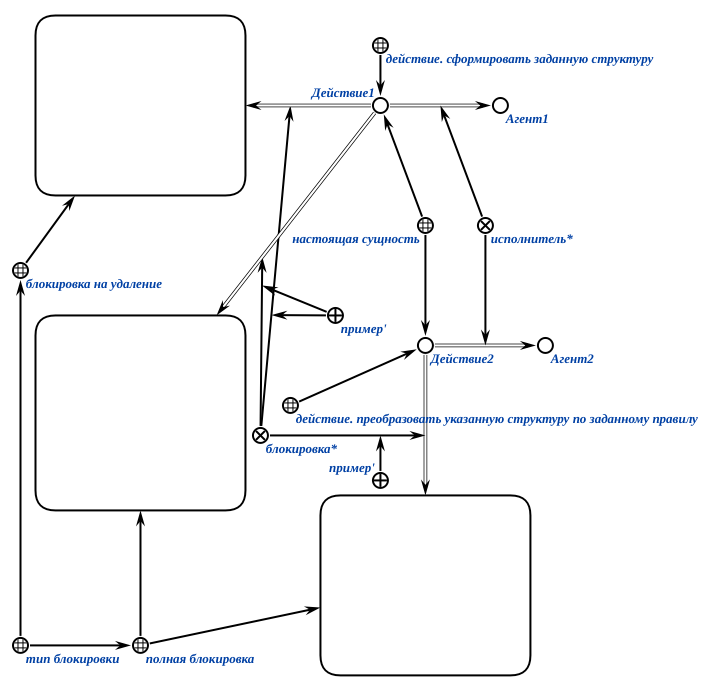
\includegraphics[scale=0.8]{images/part3/chapter_situation_management/lock.png}
	\caption{Пример использования блокировок}
	\label{fig:lock}
\end{figure}

Множество \textbf{\textit{тип блокировки}} содержит все возможные классы блокировок, т.е. \textit{структуры}, содержащие \textit{sc-элементы}, заблокированные каким-либо \textit{sc-агентом} на время выполнения им некоторого \textit{действия в sc-памяти}.

Каждая \textit{структура}, принадлежащая множеству \textbf{\textit{полная блокировка}} содержит \textit{sc-элементы}, просмотр и изменение (удаление, добавление инцидентных \textit{sc-коннекторов}, удаление самих \textit{sc-элементов}, изменение содержимого в случае файла) которых запрещены всем \textit{sc-агентам}, кроме собственно \textit{sc-агента}, выполняющего соответствующее данной структуре \textit{действие в sc-памяти}, связанное с ней отношением \textit{блокировка*}.
	
Для того, чтобы исключить возможность реализации \textit{sc-агентов}, которые могут внести изменения в конструкции, описывающие блокировки других \textit{sc-агентов}, все элементы этих конструкций, в том числе, сам знак \textit{структуры}, содержащей заблокированные \textit{sc-элементы} (принадлежащей как множеству \textbf{\textit{полная блокировка}}, так и любому другому \textit{типу блокировки}) и связки отношения \textit{блокировка*}, связывающие эту \textit{структуру} и конкретное \textit{действие в sc-памяти}, добавляются в \textbf{\textit{полную блокировку}}, соответствующую данному \textit{действию в sc-памяти}. Таким образом, каждой \textbf{\textit{полной блокировке}} соответствует петля принадлежности, связывающая ее знак с самим собой.

Каждая \textit{структура}, принадлежащая множеству \textbf{\textit{блокировка на любое изменение}} содержит \textit{sc-элементы}, изменение (физическое удаление, добавление инцидентных \textit{sc-коннекторов}, физическое удаление самих \textit{\mbox{sc-элементов}}, изменение содержимого в случае файла) которых запрещено всем \textit{sc-агентам}, кроме собственно \textit{sc-агента}, выполняющего соответствующее данной структуре \textit{действие в sc-памяти}, связанное с ней отношением \textit{блокировка*}. Однако не запрещен просмотр (чтение) этих \textit{sc-элементов} любым \textit{sc-агентом}.

Каждая \textit{структура}, принадлежащая множеству \textbf{\textit{блокировка на удаление}} содержит \textit{sc-элементы}, удаление которых запрещено всем \textit{sc-агентам}, кроме собственно \textit{sc-агента}, выполняющего соответствующее данной структуре \textit{действие в sc-памяти}, связанное с ней отношением \textit{блокировка*}. Однако не запрещен просмотр (чтение) этих \textit{sc-элементов} любым \textit{sc-агентом}, добавление инцидентных sc-коннекторов.

Рассмотрим принципы работы с блокировками:

\begin{itemize}
	\item в каждый момент времени одному процессу в sc-памяти может соответствовать только одна блокировка каждого типа;
	\item в каждый момент времени одному процессу в sc-памяти может соответствовать только одна блокировка, установленная на некоторый конкретный sc-элемент;
	\item при завершении выполнения любого процесса в sc-памяти все установленные им блокировки автоматически снимаются;
	\item для повышения эффективности работы системы в целом каждый процесс должен в каждый момент времени блокировать минимально необходимое множество sc-элементов, снимая блокировку с каждого sc-элемента сразу же, как это становится возможным (безопасным);
	\item В случае когда в рамках \textit{процесса в sc-памяти} явно выделяются более частные подпроцессы (при помощи отношений \textit{темпоральная часть*, поддействие*, декомпозиция действия*} и т. д.), то каждый такой подпроцесс с точки зрения синхронизации выполнения рассматривается как самостоятельный процесс, которому в соответствие могут быть поставлены все необходимые блокировки.
	\begin{itemize}
		\item все дочерние процессы в sc-памяти имеют доступ к блокировкам родительского процесса так же, как если бы это были блокировки соответствующие каждому из таких дочерних процессов;
		\item в свою очередь, родительский процесс не имеет какого-либо привилегированного доступа к sc-элементам, заблокированным дочерними процессами, и работает с ними так же, как любой другой процесс в sc-памяти. Исключение составляют sc-элементы, обозначающие сами дочерние процессы, поскольку родительский процесс должен иметь возможность управления дочерним, например, приостановки или прекращения их выполнения;
		\item все дочерние процессы по отношению друг к другу работают так же, как и по отношению к любым другим процессам;
		\item в случае, когда родительский процесс приостанавливает выполнение (становится \textit{отложенным действием}), \uline{все} его дочерние процессы также приостанавливают выполнение. В свою очередь, приостановка одного из дочерних процессов в общем случае не инициирует явно остановку всего родительского процесса и соответственно других дочерних.
		\end{itemize}
\end{itemize}

Рассмотрим принципы работы с \textit{полными блокировками}:
\begin{itemize}
	\item если sc-элемент, инцидентный некоторому sc-коннектору, попадает в какую-либо полную блокировку, то сам этот sc-коннектор по умолчанию также считается заблокированным этой же блокировкой. Обратное в общем случае неверно, т. к. часть sc-коннекторов, инцидентных некоторому sc-элементу, может быть полностью заблокирована, при этом сам этот элемент заблокирован не будет. Такая ситуация типична, например, для sc-узлов, обозначающих классы понятий;
	\item каждый процесс в sc-памяти может свободно изменять или удалять любые sc-элементы, попадающие в полную блокировку, соответствующую этому процессу.
\end{itemize}

Принципы работы с \textit{полными блокировками}, с одной стороны, наиболее просты, поскольку все процессы, кроме установившего такую блокировку, не имеют доступа к заблокированным \mbox{sc-элементам} и конфликты возникнуть не могут. С другой стороны, частое использование блокировок такого типа может привести к тому, что система не сможет использовать в полной мере имеющиеся у нее знания и давать неполные или даже некорректные ответы на поставленные вопросы.

Рассмотрим принципы работы с \textit{блокировками на любое изменение} и \textit{блокировками на удаление}:
\begin{itemize}
	\item на один и тот же sc-элемент в один момент времени может быть установлена только одна блокировка одного типа, но разные процессы могут одновременно установить на один и тот же элемент блокировки двух разных типов. Это касается случая, когда первый процесс установил на некоторый sc-элемент блокировку на удаление, а второй процесс затем устанавливает блокировку на любое изменение. В других случаях возникает конфликт блокировок;
	\item установка блокировки любого типа также считается изменением, таким образом, если на некоторый \mbox{sc-элемент} была установлена блокировка на любое изменение, то другой процесс не сможет установить на этот же sc-элемент блокировку любого типа, пока первый процесс не снимет свою;
	\item если блокировка на удаление устанавливается на некоторый sc-коннектор, то по умолчанию та же блокировка устанавливается на инцидентные этому sc-коннектору sc-элементы, поскольку удаление этих элементов приведет к удалению этого коннектора.
\end{itemize}

\begin{SCn}
\scnheader{процесс в sc-памяти}
\scnidtf{действие в sc-памяти}
\scnrelfrom{разбиение}{Классификация процессов в sc-памяти с точки зрения синхронизации их выполнения}
\begin{scnindent}
\begin{scneqtoset}
	\scnitem{действие поиска sc-элементов}
	\scnitem{действие генерации sc-элементов}
	\scnitem{действие удаления sc-элементов}
	\scnitem{действие установки блокировки некоторого типа на некоторый sc-элемент}
	\scnitem{действие снятия блокировки с некоторого sc-элемента}
\end{scneqtoset}
\end{scnindent}
\end{SCn}

В некоторых случаях для того, чтобы обеспечить синхронизацию, необходимо объединять несколько элементарных действий над sc-памятью в одно неделимое действие (\textbf{\textit{транзакцию в sc-памяти}}), для которого гарантируется, что ни один сторонний процесс не сможет прочитать или изменить участвующие в этом действии sc-элементы, пока действие не завершится. При этом, в отличие от ситуации с полной блокировкой, процесс, пытающийся получить доступ к таким элементам, не продолжает выполнение так, как если бы этих элементов просто не было в sc-памяти, а ожидает завершения транзакции, после чего может выполнять с данными элементами любые действия согласно общим принципам синхронизации процессов. Проблема обеспечения транзакций не может быть решена на уровне SC-кода и требует реализации таких неделимых действий на уровне \textit{платформы интерпретации sc-моделей}.

В случае выполнения \textit{действия поиска sc-элементов} все найденные и сохраненные в рамках какого-либо процесса sc-элементы попадают в соответствующую данному процессу \textit{блокировку на любое изменение}. Таким образом, гарантируется целостность фрагмента базы знаний, с которым работает некоторый процесс в sc-памяти. При этом поиск и автоматическая установка такой блокировки должны быть реализованы как \textit{транзакция в sc-памяти}.
	
Такой подход также позволяет избежать ситуации, когда один процесс заблокировал некоторый sc-элемент на любое изменение, а второй процесс пытается сгенерировать или удалить \textit{sc-коннектор}, инцидентный данному \textit{sc-элементу}. В таком случае второй процесс должен будет предварительно найти и заблокировать указанный \textit{sc-элемент} на любое изменение, что вызовет конфликт блокировок (\textit{взаимоблокировку*}).

В случае генерации любого sc-элемента в рамках некоторого процесса он автоматически попадает в полную блокировку, соответствующую данному процессу. При этом генерация и автоматическая установка такой блокировки должны быть реализованы как \textit{транзакция в sc-памяти}. При необходимости сгенерированные элементы могут быть удалены (т. е. их временное существование вообще никак не отразится на деятельности других процессов) или разблокированы в случае, когда сгенерирована информация, которая может иметь некоторую ценность в дальнейшем.

В случае если какой-либо процесс пытается установить блокировку любого типа на какой-либо sc-элемент, уже заблокированный каким-либо другим процессом, то, с одной стороны, блокировка не может быть установлена, пока другой процесс не разблокирует указанный sc-элемент; с другой стороны, для того чтобы обеспечить возможность поиска и устранения \textit{взаимоблокировок}, необходимо явно указывать тот факт, что какой-либо процесс хочет получить доступ к какому-либо заблокированному другим процессом sc-элементу. Для того чтобы иметь возможность указать, какие процессы пытаются заблокировать уже заблокированный \textit{sc-элемент}, предлагается наряду с отношением \textit{блокировка*} использовать отношение \textit{планируемая блокировка*}, полностью аналогичное отношению \textit{блокировка*}.
	
Описанный механизм регулирует также и процессы поиска, поскольку поиск и сохранение некоторого sc-элемента предполагает установку \textit{блокировки на любое изменение}. Кроме того, следует учитывать, что на один sc-элемент \textit{блокировка на любое изменение} может быть установлена после \textit{блокировки на удаление}, соответствующей другому процессу. В этом случае использовать отношение \textit{планируемые блокировки*} нет необходимости.
	
Действие проверки наличия на некотором sc-элементе блокировки и в зависимости от результата проверки, установки блокировки или планируемой блокировки (с указанием приоритета при необходимости) должно быть реализовано как транзакция.

\begin{SCn}
\scnheader{планируемая блокировка*}
\scnsubset{блокировка*}
\end{SCn}

Процесс, которому в соответствие поставлена \textit{планируемая блокировка*}, приостанавливает выполнение до тех пор, пока уже установленные блокировки не будут сняты, после чего \textit{планируемая блокировка*} становится реальной \textit{блокировкой*} и процесс продолжает выполнение в соответствии с общими правилами.

\begin{SCn}
\scnheader{приоритет блокировки*}
\scnrelfrom{область определения}{планируемая блокировка*}
\end{SCn}

В случае, когда на один и тот же sc-элемент планируют установить блокировку сразу несколько процессов, используется отношение \textit{приоритет блокировки*}, связывающее между собой пары отношения \textit{планируемая блокировка*}. Как правило, приоритет блокировки определяется тем, какой из процессов раньше попытался установить блокировку на рассматриваемый sc-элемент, хотя в общем случае приоритет может устанавливаться или меняться в зависимости от дополнительных критериев.

В случае попытки удаления некоторого sc-элемента некоторым процессом удаление может быть осуществлено только в случае, когда на данный sc-элемент не установлена (и не планируется) ни одна блокировка каким-либо другим процессом.
	
В других случаях необходимо обеспечить корректное завершение выполнения всех процессов, работающих с данным sc-элементом, и только потом удалить его физически.
	
Для реализации такой возможности каждому процессу в соответствие может быть поставлено множество удаляемых данным процессом sc-элементов.

Действие проверки наличия блокировок или планируемых блокировок на удаляемый sc-элемент и собственно его удаление или добавление во множество удаляемых sc-элементов для соответствующего процесса должно быть реализовано как транзакция.

\begin{SCn}
\scnheader{удаляемые sc-элементы*}
\scnrelfrom{первый домен}{процесс в sc-памяти}
\end{SCn}

Sc-элементы, попавшие во множество удаляемых sc-элементов некоторого процесса в sc-памяти, доступны процессам, уже установившим (или планирующим установить) на эти sc-элементы блокировки ранее (до попытки его удаления), а для всех остальных процессов эти sc-элементы уже считаются удаленными. Процесс, пытающийся удалить sc-элемент, приостанавливает свое выполнение до того момента, пока все заблокировавшие и планирующие заблокировать данный sc-элемент процессы не разблокируют его. В общем случае один sc-элемент может входить во множества удаляемых элементов одновременно для нескольких процессов, в этом случае все такие процессы одновременно продолжат выполнение после снятия с этого sc-элемента всех блокировок. Если удаление пытается осуществить один из процессов, уже установивший на указанный sc-элемент блокировку, то алгоритм действий остается прежним -- sc-элемент добавляется во множество удаляемых данным процессом sc-элементов, и будет физически удален, как только все остальные процессы, установившие на данный sc-элемент блокировки, снимут их.

Рассмотрим алгоритм снятия блокировки с некоторого sc-элемента:
\begin{enumerate}
	\item если на данный sc-элемент установлена одна или несколько \textit{планируемых блокировок*}, то первая из них по приоритету (или единственная) становится \textit{блокировкой*}, соответствующий ей процесс продолжает выполнение (становится настоящей сущностью); связка отношения приоритет выполнения, соответствовавшая удаленной связке отношения \textit{планируемая блокировка*} также удаляется, т. е. приоритет смещается на одну позицию;
	\item если \textit{планируемых блокировок*}, установленных на данный sc-элемент, нет, но он попадает во множество удаляемых sc-элементов для одного или нескольких процессов, то рассматриваемый sc-элемент физически удаляется, а приостановленные до его удаления процессы продолжают свое выполнение (становится настоящими сущностями);
	\item если на данный sc-элемент не установлены планируемые блокировки и он не входит во множество удаляемых для какого-либо процесса, то блокировка просто снимается без каких-либо дополнительных изменений.
\end{enumerate}

\begin{SCn}
\scnheader{транзакция в sc-памяти}
\begin{scnrelfromset}{разбиение}
	\scnitem{поиск некоторой конструкции в sc-памяти и автоматическая установка блокировки на любое изменение на найденные sc-элементы}
	\scnitem{генерация некоторого sc-элемента и автоматическая установка на него полной блокировки}
	\scnitem{проверка наличия на некотором sc-элементе блокировки и в зависимости от результата проверки установка блокировки или планируемой блокировки}	
	\scnitem{проверка наличия блокировок или планируемых блокировок на удаляемый sc-элемент и собственно его удаление или добавление во множество удаляемых sc-элементов для соответствующего процесса}	
	\scnitem{снятие блокировки с заданного sc-элемента и при необходимости установка первой по приоритету планируемой блокировки или удаление данного sc-элемента, если он входит во множество удаляемых sc-элементов для некоторого процесса}	
	\scnitem{поиск подпроцессов процесса и добавление их во множество отложенных действий в случае добавления самого процесса в данное множество}	
	\scnitem{поиск подпроцессов процесса и удаление их из множества отложенных действий в случае удаления самого процесса из данного множества}	
\end{scnrelfromset}
\end{SCn}

При реализации \textit{абстрактных программных sc-агентов} на \textit{языке SCP}, соблюдение всех принципов синхронизации соответствующих этим sc-агентам процессов обеспечивается на уровне \textit{sc-агентов интерпретации scp-программ}, т. е. средствами \textit{платформы интерпретации sc-моделей}. При реализации \textit{абстрактных программных sc-агентов} на уровне платформы, соблюдение всех принципов синхронизации возлагается, во-первых, непосредственно на разработчика агентов, во-вторых, -- на разработчика платформы. Так, например, платформа может предоставлять доступ к хранимым в sc-памяти элементам через некоторый программный интерфейс, уже учитывающий принципы работы с блокировками, что избавит разработчика агентов от необходимости учитывать все эти принципы вручную.

Кроме того, выделяется ряд специфичных принципов работы \textit{абстрактных программных sc-агентов}, реализованных на \textit{языке SCP}:
\begin{itemize}
\item в результате появления в sc-памяти некоторой конструкции, удовлетворяющей условию инициирования какого-либо \textit{абстрактного sc-агента}, реализованного при помощи \textit{Языка SCP}, в \textit{sc-памяти} генерируется и инициируется \textit{scp-процесс}. В качестве шаблона для генерации используется \textit{агентная scp-программа}, соответствующая данному \textit{абстрактному sc-агенту}.
\item каждый такой \textit{scp-процесс}, соответствующий некоторой \textit{агентной \mbox{scp-программе}}, может быть связан с набором структур, описывающих блокировки различных типов. Таким образом, синхронизация взаимодействия параллельно выполняемых \textit{scp-процесcов} осуществляется так же, как и в случае любых других \textit{действий в sc-памяти}.
\item несмотря на то что каждый \textit{scp-оператор} представляет собой атомарное действие в sc-памяти, являющееся поддействием в рамках всего \textit{\mbox{scp-процесса}}, блокировки, соответствующие одному оператору, не вводятся, чтобы избежать громоздкости и избытка дополнительных системных конструкций, создаваемых при выполнении некоторого \textit{scp-процесса}. Вместо этого используются блокировки, общие для всего \textit{scp-процесса}. Таким образом, \textit{агенты интерпретации scp-программ} работают только с учетом блокировок, общих для всего интерпретируемого \textit{scp-процесса}.
\item процессы, описывающие деятельность агентов интерпретации \textit{scp-программ}, как правило, не создаются, следовательно, и не вводятся соответствующие им блокировки. Поскольку такие агенты работают с уникальным scp-процессом и их число ограничено и известно, то использование блокировок для их синхронизации не требуется.
\item в случае приостановки \textit{scp-процесса} (добавления его во множество \textit{отложенных действий}) в соответствии с общими правилами синхронизации все его дочерние процессы также должны быть	приостановлены. В связи с этим все \textit{scp-операторы}, которые в	этот момент являются \textit{настоящими сущностями}, становятся	\textit{отложенными действиями}.
\item во избежание нежелательных изменений в самом теле \textit{scp-процесса}, вся конструкция, сгенерированная на основе некоторой \textit{scp-программы} (весь \textit{sc-текст}, описывающий декомпозицию \textit{scp-процесса} на \textit{scp-операторы}), должна быть добавлена в \textit{полную блокировку}, соответствующую данному \textit{scp-процессу}.
\item при необходимости разблокировать или заблокировать некоторую конструкцию каким-либо типом блокировки используются соответствующие \textit{scp-операторы} класса \textit{scp-оператор управления блокировками}.
\item после завершения выполнения некоторого scp-процесса его текст, как правило, удаляется из \textit{sc-памяти}, а все заблокированные конструкции освобождаются (разрушаются знаки структур, обозначавших блокировки).
\item как правило, частный \textit{класс действий}, соответствующий конкретной \textit{scp-программе}, явно не вводится, а используется более общий класс \textit{scp-процесс}, за исключением тех случаев, когда введение	специального \textit{класса действий} необходимо по каким-либо другим соображениям.
\end{itemize}

В общем случае весь механизм блокировок может описываться как на уровне SC-кода (для повышения уровня платформенной независимости), так и при необходимости может быть реализован на уровне \textit{платформы интерпретации sc-моделей}, например для повышения производительности. Для этого каждому выполняемому в sc-памяти процессу на нижнем уровне может быть поставлена в соответствие некая уникальная таблица, в каждый момент времени содержащая перечень заблокированных элементов с указанием типа блокировки.

Рассмотрим пример применения описанного механизма.

\begin{figure}[h]
	\centering
	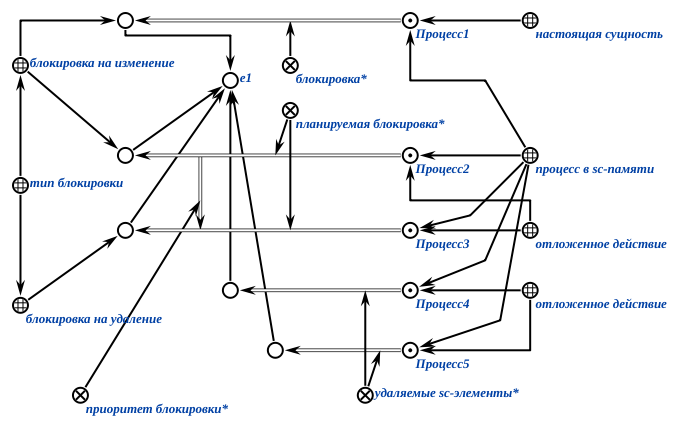
\includegraphics[scale=0.8]{images/part3/chapter_situation_management/plan_lock_1.png}
	\caption{Пример использования планируемых блокировок}
	\label{fig:plan_lock_1}
\end{figure}

В данном примере \textit{Процесс1} непосредственно работает с sc-элементом \textit{\textbf{e1}},\textit{Процесс2} и \textit{Процесс3} планируют установить блокировку на любое изменение и блокировку на удаление соответственно, причем \textit{Процесс2} попытался установить свою блокировку раньше, чем \textit{Процесс3}, поэтому согласно направлению связки отношения \textit{приоритет блокировки*}, его блокировка будет установлена раньше. \textit{Процесс4} и \textit{Процесс5} ожидают снятия всех блокировок и планируемых блокировок, после чего \textit{\textbf{e1}} будет удален и \textit{Процесс1} и \textit{Процесс2} продолжат свое выполнение. Никакие другие планируемые блокировки установлены быть уже не могут, поскольку \textit{\textbf{e1}} попал во множество удаляемых sc-элементов как минимум одного процесса и, в соответствии с изложеннымивыше правилами, все остальные процессы кроме \textit{Процесс1}-\textit{Процесс5}, уже несмогут получить доступ к этому sc-элементу.		
Выполняемый процесс принадлежит множеству настоящая сущность, приостановленные -- множеству отложенное действие.

\begin{figure}[h]
	\centering
	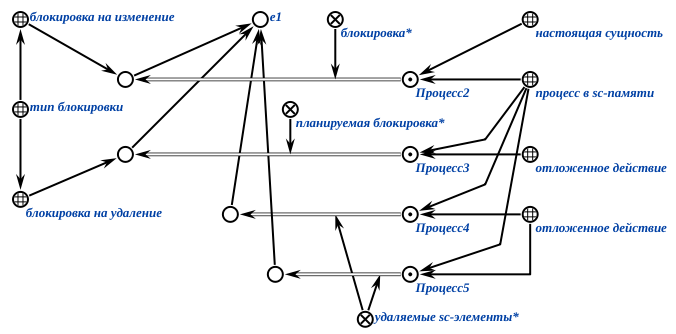
\includegraphics[scale=0.8]{images/part3/chapter_situation_management/plan_lock_2.png}
	\caption{Пример использования планируемых блокировок (продолжение)}
	\label{fig:plan_lock_2}
\end{figure}

После того как \textit{Процесс1} разблокировал sc-элемент \textit{\textbf{e1}}, этот элемент будет заблокирован \textit{Процессом2}, и \textit{Процесс2} продолжит выполнение. \textit{Планируемая блокировка*}, установленная \textit{Процессом2}, становится обычной \textit{блокировкой*}.

\begin{figure}[h]
	\centering
	\includegraphics[scale=0.8]{images/part3/chapter_situation_management/plan_lock_3.png}
	\caption{Пример использования блокировки на удаление}
	\label{fig:plan_lock_3}
\end{figure}

После того как \textit{Процесс2} разблокировал sc-элемент \textit{\textbf{e1}}, этот элемент будет заблокирован \textit{Процессом3}, и \textit{Процесс3} продолжит выполнение.

\begin{figure}[h]
	\centering
	\includegraphics[scale=0.8]{images/part3/chapter_situation_management/plan_lock_4.png}
	\caption{Удаляемые sc-элементы}
	\label{fig:plan_lock_4}
\end{figure}

Когда все процессы снимут блокировки с sc-элемента \textit{\textbf{e1}}, он может быть физически удален и \textit{Процесс4} и \textit{Процесс5} продолжат выполнение.

В зависимости от конкретных \textit{типов блокировок} установленных паралельно выполняемыми процессами на некоторые sc-элементы и того, какие конкретно действия с этими \textit{sc-элементами} предполагается выполнить далее в рамках выполнения этих процессов, возможны ситуации взаимоблокировки, когда каждый из указанных процессов будет ожидать снятия блокировки вторым процессом с нужного \textit{sc-элемента}, не снимая при этом установленной им самим блокировки с \textit{sc-элемента}, доступ к которому необходим второму процессу.
	
В случае когда хотя бы одна из блокировок является \textit{полной блокировкой}, ситуация взаимоблокировки возникнуть не может, поскольку \textit{sc-элементы}, попавшие в \textit{полную блокировку} некоторого \textit{scp-процесса}, не доступны другим \textit{scp-процессам} даже для чтения и, таким образом, остальные \textit{scp-процессы} будут работать так, как будто заблокированные \textit{sc-элементы} просто отсутствуют в текущем состоянии \textit{sc-памяти}.

В случаях, когда ни одна из установленных блокировок не является \textit{полной блокировкой}, возможно появление взаимоблокировок.

Устранение \textit{взаимоблокировки} невозможно без вмешательства специализированного \textit{sc-метаагента}, который имеет право игнорировать блокировки, установленные другими процессами. 
	
В общем случае проблема конкретной взаимоблокировки может быть решена путем выполнения специализированным \textit{sc-метаагентом} следующих шагов:	
\begin{itemize}
	\item откат нескольких операций, выполненных одним из участвующих в взаимоблокировке процессов настолько шагов назад, насколько это необходимо для того, чтобы второй процесс получил доступ к необходимым \textit{sc-элементам} и смог продолжить выполнение;
	\item ожидание выполнения второго процесса вплоть до завершения или до снятия им всех блокировок с \textit{sc-элементов}, доступ к которым необходимо получить первому процессу;
	\item повторное выполнение в рамках первого процесса отмененных операций и продолжение его выполнения, но уже с учетом изменений в памяти, внесенных вторым процессом.		
\end{itemize}

Для \textit{sc-метаагентов} все sc-элементы, в том числе описывающие блокировки, планируемые блокировки и т. д. полностью эквивалентны между собой с точки зрения доступа к ним, т. е. любой \textit{sc-метаагент} имеет доступ к любым sc-элементам, даже попавшим в полную блокировку для какого-либо другого процесса. Это необходимо для того, чтобы \textit{sc-метаагенты} смогли выявлять и устранять различные проблемы, например, описанную выше проблему взаимоблокировки.

Таким образом, проблема синхронизации деятельности \textit{sc-метаагентов} требует введения дополнительных правил.

Указанную проблему разделим на две более частные:
\begin{itemize}
	\item обеспечение синхронизации деятельности \textit{sc-метаагентов} между собой;
	\item обеспечение синхронизации деятельности \textit{sc-метаагентов} и \textit{программных sc-агентов}.		
\end{itemize}

Первую проблему предлагается решить за счет запрета параллельного выполнения \textit{sc-метаагентов}. Таким образом, в каждый момент времени в рамках одной \textit{ostis-системы} может существовать только один процесс, соответствующий \textit{sc-метаагенту} и являющийся \textit{настоящей сущностью}. 

Вторую проблему предлагается решить за счет введения дополнительных привилегий для \textit{sc-метаагентов} при обращении к какому-либо sc-элементу. Для этого достаточно одного правила: 

Если некоторый sc-элемент стал использоваться в рамках процесса, соответствующего \textit{sc-метаагенту} (например, стал элементом хотя бы одного scp-оператора, входящего в данный процесс), то все процессы, в блокировки соответствующие которым попадает указанный sc-элемент, становятся отложенными действиями (приостанавливают выполнение). Как только указанный sc-элемент перестает использоваться в рамках процесса, соответствующего \textit{sc-метаагенту}, все приостановленные по этой причине процессы продолжают выполнение.

Рассмотренные ограничения не ухудшают производительность ostis-системы существенно, поскольку \textit{sc-метаагенты} предназначены для решения достаточно узкого класса задач, которые, как показал опыт практической разработки прототипов различных \textit{ostis-систем}, возникают достаточно редко.
	
Стоит отметить, что возможна ситуация, при которой выполнение некоторого процесса в sc-памяти прервано по причине возникновения какой-либо ошибки. В таком случае существует вероятность того, что блокировка, установленная данным процессом не будет снята до тех пор, пока этого не сделает sc-метаагент, обнаруживший подобную ситуацию. Однако указанная проблема на уровне sc-модели может быть решена лишь частично, для случаев, когда ошибка возникает при интерпретации scp-программы, отслеживается scp-интепретатором и в памяти формируется соответствующая конструкция, сообщающая о проблеме sc-метаагенту. Случаи, когда возникла ошибка на уровне scp-интерпретатора или sc-хранилища, должны рассматриваться на уровне платформы интерпретации sc-моделей.

\section{Базовый язык программирования ostis-систем}
\subsection{Синтаксис Базового языка программирования ostis-систем}
\subsection{Денотационная семантика Базового языка программирования ostis-систем}
\subsection{Операционная семантика Базового языка программирования ostis-систем}

%\input{author/references}
\chapter{Язык вопросов для ostis-систем}
\chapauthortoc{Самодумкин С.~А.\\Зотов Н.~В.\\Шункевич Д.~В.\\ Ивашенко В.~П.}
\label{chapter_requests}

\vspace{-7\baselineskip}

\begin{SCn}
\begin{scnrelfromlist}{авторы}
	\scnitem{Самодумкин С.~А.}
	\scnitem{Зотов Н.~В.}
	\scnitem{Шункевич Д.~В.}
	\scnitem{Ивашенко В.~П.}
\end{scnrelfromlist}

\bigskip

\scntext{аннотация}{Возможности \textit{баз знаний} \textit{ostis-систем} позволяют не только представлять и структурировать знания об окружающем мире, но и быстро получать и формировать эти знания о нем, тем самым удовлетворяя информационную потребность пользователя. В данной главе уточнена формальная спецификация \textit{Языка вопросов для ostis-систем}, позволяющая описывать и интерпретировать любые классы \textit{вопросов} \textit{пользователей ostis-систем}.}

\bigskip

\begin{scnrelfromlist}{подраздел}
	\scnitem{\ref{sec_requests_syntax}~\nameref{sec_requests_syntax}}
	\scnitem{\ref{sec_requests_den_semantics}~\nameref{sec_requests_den_semantics}}
	\scnitem{\ref{sec_requests_op_semantics}~\nameref{sec_requests_op_semantics}}
\end{scnrelfromlist}

\bigskip

\begin{scnrelfromlist}{ключевое понятие}
	\scnitem{вопрос}
	\scnitem{ответ на вопрос}
	\scnitem{знак в рамках заданного вопроса}
	\scnitem{основной знак в рамках заданного вопроса}
	\scnitem{неосновной знак в рамках заданного вопроса}
	\scnitem{отношение в рамках заданного вопроса}
	\scnitem{базовое отношение в рамках заданного вопроса}
	\scnitem{интерпретатор Языка вопросов для ostis-систем}
\end{scnrelfromlist}

\begin{scnrelfromlist}{ключевой знак}
	\scnitem{Язык вопросов для ostis-систем}
	\scnitem{Синтаксис Языка вопросов для ostis-систем}
	\scnitem{Денотационная семантика Языка вопросов для ostis-систем}
	\scnitem{Семантическая классификация вопросов}
	\scnitem{Операционная семантика Языка вопросов для ostis-систем}
\end{scnrelfromlist}

\bigskip

\begin{scnrelfromlist}{библиографическая ссылка}
	\scnitem{\scncite{Averyanov1993}}
	\scnitem{\scncite{Suleimanov2001}}
	\scnitem{\scncite{Suleimanov2014}}
	\scnitem{\scncite{Bukharev1990}}
	\scnitem{\scncite{Kwok2001}}
	\scnitem{\scncite{Emelyanov2007}}
	\scnitem{\scncite{Finn1976}}
	\scnitem{\scncite{Finn1981}}
	\scnitem{\scncite{Belnap1981}}
	\scnitem{\scncite{Sosnin2007}}
	\scnitem{\scncite{Zaharov2002}}
	\scnitem{\scncite{Hant1978}}
	\scnitem{\scncite{Lyubarsky1990}}
	\scnitem{\scncite{Samodumkin2009}}
	\scnitem{\scncite{Samodumkin2009a}}
\end{scnrelfromlist}
	
\end{SCn}

\section*{Введение в Главу \ref{chapter_requests}}

Одна из ключевых особенностей \textit{интеллектуальной системы} состоит в том, что \textit{пользователь} имеет возможность формулировать свою информационную потребность. Cпособом выражения такой потребности является \textit{вопрос}. В процессе общения всегда существует контекст, который определяет дополнительную информацию, способствующую правильному пониманию \textit{смысла} сообщения. Особенность представления информации в \textit{базах знаний} \textit{ostis-систем} упрощает формирование информационной потребности пользователя, так как представленная информация в \textit{базах знаний} уже структурирована и известны отношения, заданные на определенном понятии, в отношении которого разрешается вопросно-проблемная ситуация. В работе \scncite{Averyanov1993} показано, что вопросно-проблемная ситуация не может быть решена в рамках формальной логики и природа вопроса может быть понятна в системе субъектно-объектных отношений. В связи с тем, что при формировании \textit{баз знаний} \textit{ostis-систем} происходит формирование субъектно-объектных отношений в рамках заданной \textit{предметной области}, тем самым упрощается выражение информационной потребности пользователем средствами \textit{SC-кода}.   

Целью разработки \textbf{\textit{Языка вопросов для ostis-систем}} и последующего его развития является реализация возможности понимания действий, осуществляемых \textit{ostis-системой}, при формировании ответа на поставленный \textit{вопрос}. В процессе формирования ответа на поставленный \textit{вопрос} возможны следующие варианты:
\begin{textitemize}
	\item \textit{ответ на} поставленный \textit{вопрос} существует в \textit{базе знаний} и происходит локализация \textit{фрагмента базы знаний} в контексте выраженной средствами \textit{SC-кода} информационной потребности \textit{пользователя};
	\item ответ связан с разрешением некоторой задачной ситуации, которая содержится в контексте \textit{вопроса} и формирование \textit{ответа на вопрос} возлагается на \textit{решатель задач} (см. \textit{Главу \ref{chapter_situation_management}~\nameref{chapter_situation_management}}).
\end{textitemize}

\begin{SCn}
\scnheader{Язык вопросов для ostis-систем}
\scnidtf{Предлагаемый нами вариант языка для описания вопросов и ответов на них в ostis-системах}
\scniselement{sc-язык}
\scnrelfrom{синтаксис языка}{Синтаксис Языка вопросов для ostis-систем}
\begin{scnindent}
	\scnsubset{Синтаксис SC-кода}
\end{scnindent}
\scnrelfrom{денотационная семантика языка}{Денотационная семантика Языка вопросов для ostis-систем}
\begin{scnindent}
	\scnidtf{Онтология классов знаков и отношений для описания формулировок вопросов на SC-коде}
	\scnsuperset{Семантическая классификация вопросов}
\end{scnindent}
\scnrelfrom{операционная семантика языка}{Операционная семантика Языка вопросов для ostis-систем}
\begin{scnindent}
	\scnidtf{Коллектив sc-агентов вывода ответов на заданные вопросы пользователя ostis-системы}
\end{scnindent}
\end{SCn}

\section{Синтаксис Языка вопросов для ostis-систем}
\label{sec_requests_syntax}

\textit{Язык вопросов для ostis-систем} относится к семейству семантических совместимых языков --- \textit{sc-языков} и предназначен для формального описания поискового предписания \textit{ostis-систем} с целью удовлетворения информационной потребности \textit{пользователя}. Поэтому \textbf{\textit{Синтаксис Языка вопросов для ostis-систем}}, как и \textit{синтаксис} любого другого \textit{sc-языка}, является \textit{Синтаксисом SC-кода}. Такой подход позволяет:
\begin{textitemize}
	\item унифицировать форму представления \textit{вопросов} и \textit{знаний}, с помощью которых строятся ответы на поставленные \textit{вопросы};
	\item использовать минимум средств для интерпретации заданных \textit{вопросов пользователей};
	\item сводить формирование ответов на большую часть заданных \textit{вопросов} к поиску информации в текущем состоянии \textit{базы знаний ostis-системы}.
\end{textitemize}

\section{Денотационная семантика Языка вопросов для ostis-систем}
\label{sec_requests_den_semantics}

\begin{SCn}
\begin{scnrelfromlist}{ключевое понятие}
	\scnitem{вопрос}
	\scnitem{ответ на вопрос}
	\scnitem{знак в рамках заданного вопроса}
	\scnitem{основной знак в рамках заданного вопроса}
	\scnitem{неосновной знак в рамках заданного вопроса}
	\scnitem{отношение в рамках заданного вопроса}
	\scnitem{базовое отношение в рамках заданного вопроса}
\end{scnrelfromlist}
\end{SCn}

\textbf{\textit{Денотационная семантика Языка вопросов для ostis-систем}} включает \textit{классы вопросов} и соответствующие \textit{классы ответов}, необходимые для спецификации формулировок \textit{вопросов} и \textit{ответов} на них, а также \textit{классы знаков} и \textit{отношений}, входящих в структуру любого \textit{вопроса}. В \textit{Семантической классификации вопросов} \textit{Языка вопросов для ostis-систем} заложена идея, описанная в работе \scncite{Suleimanov2001}.

Любой \textbf{\textit{вопрос}} на \textit{Языке вопросов для ostis-систем} представляет собой \textit{спецификацию действия} на поиск или синтез \textit{знания}, удовлетворяющего информационную потребность \textit{пользователя}, инициирующего этот \textit{вопрос}. То есть \textit{вопрос} --- это ничто иное как \textit{задача}, с помощью которой выражается потребность пользователя в некоторой информации, возможно хранимой или выводимой в \textit{базе знаний} \textit{ostis-системы} (см. \textit{Главу \ref{chapter_actions}~\nameref{chapter_actions}}). 

Каждому \textit{вопросу} можно взаимно однозначно сопоставить некоторое множество \textit{ответов на} этот \textit{вопрос}. Каждый \textit{ответ на вопрос} представляет собой некоторую \textit{sс-структуру} \textit{семантической окрестности основного знака}, раскрываемого в этом \textit{ответе на} заданный \textit{вопрос}.

\begin{SCn}
\scnheader{вопрос}
\scnidtf{запрос}
\scnidtf{непроцедурная формулировка задачи на поиск (в текущем состоянии базы знаний) или на синтез знания, удовлетворяющего заданным требованиям}
\scnidtf{запрос метода (способа) решения заданного (указываемого) \textit{класса задач} либо \textit{плана решения} конкретной указываемой \textit{задачи}}
\scnidtf{задача, направленная на удовлетворение информационной потребности некоторого субъекта-заказчика}
\scnsubset{задача}

\scnheader{ответ на вопрос}
\scnidtf{ответ на запрос}
\scnidtf{результат запроса}
\scnidtf{результат решения задачи на поиск или синтез знания, удовлетворяющий заданным требованиям}
\scnidtf{семантическая окрестность \textit{основного знака}, знание в которой удовлетворяет информационную потребность пользователя}
\scnidtf{знание в базе знаний ostis-системы, которое удовлетворяет информационную потребность пользователя}
\scnsubset{знание}
\end{SCn}

Среди всех классов \textit{знаков в рамках заданного вопроса} \textit{Языка вопросов для ostis-систем} можно выделить наиболее общие по иерархии классы \textit{знаков}:

\begin{SCn}
\scnheader{знак в рамках заданного вопроса}
\scnsubset{знак}
\begin{scnrelfromset}{разбиение}
	\scnitem{основной знак в рамках заданного вопроса}
	\begin{scnindent}
		\scnidtf{ключевой sc-элемент в рамках заданного вопроса}
		\scnidtf{\textit{знак}, относительно которого задан вопрос}
	\end{scnindent}
	\scnitem{неосновной знак в рамках заданного вопроса}
	\begin{scnindent}
		\scnidtf{\textit{знак}, стоящий в некотором отношении с \textit{основным знаком в рамках заданного вопроса}}
	\end{scnindent}
\end{scnrelfromset}
\end{SCn}

\textbf{\textit{знаком в рамках заданного вопроса}} является любой \textit{знак понятия} или \textit{сущности}, принадлежащий этому \textit{вопросу}. Между \textit{знаками в рамках заданного вопроса} задается множество связей \textit{отношений}, входящих в состав различных \textit{предметных областей}. Кроме того, любое \textbf{\textit{отношение в рамках заданного вопроса}} представляет собой \textit{отношение} между \textit{знаками} \textit{предметной области}, принадлежащих заданному \textit{вопросу}. Среди всех классов \textit{отношений в рамках заданного вопроса} можно выделить класс \textbf{\textit{базовых отношений в рамках заданного вопроса}} и класс \textbf{\textit{составных отношений в рамках заданного вопроса}}.

\begin{SCn}
\scnheader{отношение в рамках заданного вопроса}
\scnidtf{определенное отношение между знаками \textit{предметной области} в контексте \textit{вопроса}}
\scnsubset{отношение}

\scnheader{базовое отношение в рамках заданного вопроса}
\scnidtf{\textit{класс отношений}, объединяющий \textit{отношения в заданном вопросе}, отражающие однотипный \textit{смысл} и раскрывающие определенный признак \textit{знаков} \textit{предметной области}}
\scnsubset{отношение в рамках заданного вопроса}
\begin{scnrelfromset}{декомпозиция}
	\scnitem{отношение состояния}
	\scnitem{отношение действия}
	\scnitem{отношение состава}
	\scnitem{теоретико-множественное отношение}
	\scnitem{темпоральное отношение}
	\scnitem{пространственное отношение}
	\scnitem{количественное отношение}
	\scnitem{качественное отношение}
\end{scnrelfromset}
\end{SCn}

Например, \textit{отношения в рамках заданного вопроса} такие, как \scnqqi{играет*}, \scnqqi{спит*}, \scnqqi{плавает*}, объединяются в класс \textit{отношений состояния} по признаку выражать состояние знака (то есть данные отношения раскрывают признак \textit{знака} \textit{предметной области} --- \scnqqi{находиться в некотором состоянии}).

\begin{SCn}
\scnheader{составное отношение в рамках заданного вопроса}
\scnidtf{устойчивая комбинация двух \textit{отношений действия}: действия, направленного на \textit{параметр вопроса\scnrolesign}, и действия, направленного на \textit{ответ на вопрос*}}
\end{SCn}

Например, элемент \textit{составного отношения в рамках заданного вопроса} между \textit{знаками}: \scnqqi{\textit{Нефтеперерабатывающий завод}}, \scnqqi{\textit{нефть}} и \scnqqi{\textit{нефтепродукты}} --- может быть представлен как \scnqqi{Нефтеперерабатывающий завод перерабатывает нефть в нефтепродукты}.

Смысловая классификация \textit{вопросов} дает возможность противопоставить каждому типу вопроса ограниченный набор допустимых, то есть \textit{семантически корректных информационных конструкций}, передающий правильный \textit{смысл} \textit{вопроса} в зависимости от класса \textit{вопроса}. При этом \textbf{\textit{Семантическая классификация вопросов}} позволяет разбить множество \textit{вопросов} на классы, в каждом из которых требуется раскрытие некоторого однотипного \textit{смысла}, заданного классом этого \textit{вопроса}. 

\begin{SCn}
\scnheader{вопрос}
\begin{scnrelfromset}{декомпозиция}
	\scnitem{вопрос, требующий вывода семантической окрестности \textit{основного знака}}
	\begin{scnindent}
		\begin{scnhaselementrolelist}{пример}
			\scnitem{Вопрос. Что такое \textit{Город Минск}}
		\end{scnhaselementrolelist}
	\end{scnindent}
	\scnitem{вопрос, требующий раскрытия в ответе \textit{базового отношения} \textit{основного знака}}
	\begin{scnindent}
		\begin{scnhaselementrolelist}{пример}
			\scnitem{Вопрос. Что легче: железо или дерево}
		\end{scnhaselementrolelist}
	\end{scnindent}
	\scnitem{вопрос, требующий раскрытия в ответе \textit{составного отношения} \textit{основного знака}}
	\begin{scnindent}
		\scntext{пояснение}{Такому классу \textit{вопросов} соответствуют классы \textit{ответов}, в которых \textit{главный знак} раскрывается через \textit{составное отношение}.}
		\begin{scnhaselementrolelist}{пример}
			\scnitem{Вопрос. Какие Принципы компонентного проектирования в интеллектуальных компьютерных системах нового поколения}
		\end{scnhaselementrolelist}
	\end{scnindent}
	\scnitem{вопрос, требующий раскрытия в ответе произвольной комбинации \textit{базового отношения} и/или \textit{составного отношения} \textit{основного знака}}
	\begin{scnindent}
		\begin{scnhaselementrolelist}{пример}
			\scnitem{Вопрос. Как определяется уровень интеллекта кибернетической системы}
		\end{scnhaselementrolelist}
	\end{scnindent}
	\scnitem{вопрос, требующий раскрытия в ответе более чем одного \textit{основного знака}}
	\begin{scnindent}
		\begin{scnhaselementrolelist}{пример}
			\scnitem{Вопрос. Докажите теорему Пифагора}
		\end{scnhaselementrolelist}
	\end{scnindent}
\end{scnrelfromset}
\end{SCn}

\begin{SCn}
\scnheader{вопрос, требующий раскрытия в ответе \textit{базового отношения} \textit{основного знака}}
\begin{scnrelfromset}{декомпозиция}
	\scnitem{вопрос, требующий раскрытия в ответе \textit{отношения состава} \textit{основного знака}}
	\begin{scnindent}
		\scnidtf{класс вопросов, в ответах на которые \textit{основной знак} \textit{S} раскрывается через его \textit{отношение состава} в связке с его составляющими знаками \textit{P} и \textit{Q}}
		\begin{scnhaselementrolelist}{пример}
			\scnitem{Вопрос. Какие административные районы входят в состав Города Витебск}
			\begin{scnindent}
				\scneqimage[30em]{author/part3/figures/question\_about\_vitebsk\_regions.png}
				\scnrelfrom{ответ на вопрос}{\{Железнодорожный район Города Витебск, Октябрьский район Города Витебск, Первомайский район Города Витебск\}}
				\begin{scnindent}
					\scneqimage[30em]{author/part3/figures/question\_about\_vitebsk\_regions\_answer.png}
				\end{scnindent}
			\end{scnindent}
		\end{scnhaselementrolelist}
	\end{scnindent}
	\scnitem{вопрос, требующий раскрытия в ответе \textit{теоретико-множественного отношения} \textit{основного знака}}
	\begin{scnindent}
		\scnidtf{класс вопросов, в ответах на которые \textit{основной знак} \textit{S} раскрывается через его \textit{теоретико-множественное отношение} в связке с другим знаком \textit{P}, содержащего \textit{S} как часть}
		\begin{scnhaselementrolelist}{пример}
			\scnitem{Вопрос. Частью какой области является Смолевичский район}
			\begin{scnindent}
				\scneqimage[30em]{author/part3/figures/question\_about\_smolevichi\_inclusion.png}
				\scnrelfrom{ответ на вопрос}{\{Смолевичский район является частью Минской области\}}
			\end{scnindent}
		\end{scnhaselementrolelist}
	\end{scnindent}
	\scnitem{вопрос, требующий раскрытия в ответе \textit{отношения состояния} \textit{основного знака}}
	\begin{scnindent}
		\scnidtf{класс вопросов, в ответах на которые \textit{основной знак} \textit{S} раскрывается через его \textit{отношение состояния}}
		\begin{scnhaselementrolelist}{пример}
			\scnitem{Вопрос. Какие города современной территории Республики Беларусь имели Магдебургское право}
			\begin{scnindent}
				\scneqimage[30em]{author/part3/figures/question\_about\_minsk\_district\_town\_with\_mag\_act.png}
				\scnrelfrom{ответ на вопрос}{\{Волковыск, Гродно, Мозырь и другие имели Магдебургское право\}}
			\end{scnindent}
		\end{scnhaselementrolelist}
	\end{scnindent}
	\scnitem{вопрос, требующий раскрытия в ответе \textit{отношения действия} \textit{основного знака}}
	\begin{scnindent}
		\scnidtf{класс вопросов, в ответах на которые \textit{основной знак} \textit{S} раскрывается через его \textit{отношение действия} в связке с другим знаком \textit{P}}
	\end{scnindent}
	\scnitem{вопрос, требующий раскрытия в ответе \textit{темпорального отношения} \textit{основного знака}}
	\begin{scnindent}
		\scnidtf{класс вопросов, в ответах на которые \textit{основной знак} \textit{S} раскрывается через его \textit{темпоральное отношение} в связке с другим знаком \textit{P} по некоторой временной шкале}
		\begin{scnhaselementrolelist}{пример}
			\scnitem{Вопрос. Какое событие произошло раньше: Первый раздел Речи Посполитой или Бородинское сражение}
			\begin{scnindent}
				\scneqimage[30em]{author/part3/figures/question\_about\_events.png}
				\scnrelfrom{ответ на вопрос}{\{Первый раздел Речи Посполитой был раньше Бородинского сражения\}}
				\begin{scnindent}
					\scneqimage[30em]{author/part3/figures/question\_about\_event\_answer.png}
				\end{scnindent}
			\end{scnindent}
		\end{scnhaselementrolelist}
	\end{scnindent}
	\scnitem{вопрос, требующий раскрытия в ответе \textit{пространственного отношения} \textit{основного знака}}
	\begin{scnindent}
		\scnidtf{класс вопросов, в ответах на которые \textit{основной знак} \textit{S} раскрывается через \textit{пространственное отношение}, отражающее его положение в пространстве относительно другого знака \textit{P}}
	\end{scnindent}
	\scnitem{вопрос, требующий раскрытия в ответе \textit{количественного отношения} \textit{основного знака}}
	\begin{scnindent}
		\scnidtf{класс вопросов, в ответах на которые раскрывается \textit{количественное отношение} \textit{основного знака}}
		\begin{scnhaselementrolelist}{пример}
			\scnitem{Вопрос. Какова высота Горы Дзержинская}
			\begin{scnindent}
				\scneqimage[30em]{author/part3/figures/question\_about\_mountain\_length.png}
				\scnrelfrom{ответ на вопрос}{\{Высота Горы Дзержинская --- 345 м\}}
			\end{scnindent}
		\end{scnhaselementrolelist}
	\end{scnindent}
	\scnitem{вопрос, требующий раскрытия в ответе \textit{качественного отношения} \textit{основного знака}}
	\begin{scnindent}
		\scnidtf{класс вопросов, в ответах на которые раскрывается \textit{качественное отношение} \textit{основного знака} \textit{S} в связке с другим знаком \textit{P}}
		\begin{scnhaselementrolelist}{пример}
			\scnitem{Вопрос. Территория какой административной области больше: Минской или Брестской}
			\begin{scnindent}
				\scneqimage[30em]{author/part3/figures/question\_about\_district\_squares.png}
				\scnrelfrom{ответ на вопрос}{\{Территория Минской области больше Брестской\}}
				\begin{scnindent}
					\scneqimage[30em]{author/part3/figures/question\_about\_district\_squares\_answer.png}
				\end{scnindent}
			\end{scnindent}
		\end{scnhaselementrolelist}
	\end{scnindent}
\end{scnrelfromset}
\end{SCn}

\begin{SCn}
\scnheader{вопрос, требующий раскрытия в ответе произвольной комбинации \textit{базового отношения} и/или \textit{составного отношения} \textit{основного знака}}
\begin{scnrelfromset}{декомпозиция}
	\scnitem{вопрос, требующий раскрытия в ответе произвольной комбинации \textit{составного отношения описания} \textit{основного знака}}
	\begin{scnindent}
		\scnidtf{класс вопросов, в ответах на которые раскрываются произвольные комбинации \textit{базового отношения} и/или \textit{составного отношения} \textit{основного знака} \textit{S} в связке с другими знаками}
		\begin{scnhaselementrolelist}{пример}
			\scnitem{\{S состоит из P, Q, W. S переводит X и Y и выполняется раньше Z\}}
			\begin{scnindent}
				\scnrelto{ответ на вопрос}{Вопрос. Что такое S}
			\end{scnindent}
		\end{scnhaselementrolelist}
	\end{scnindent}
	\scnitem{вопрос, требующий раскрытия в ответе произвольной комбинации \textit{составного отношения определения} \textit{основного знака}}
	\begin{scnindent}
		\scnidtf{класс ответов, в которых \textit{основной знак} \textit{S} раскрывается через \textit{первостепенное понятие} и его \textit{описание}}
		\begin{scnhaselementrolelist}{пример}
			\scnitem{\{Минск --- это столица, которая находится в РБ\}}
			\begin{scnindent}
				\scnrelto{ответ на вопросы}{Вопрос. Как определяется город Минск}
			\end{scnindent}
		\end{scnhaselementrolelist}
	\end{scnindent}
	\scnitem{вопрос, требующий раскрытия в ответе произвольной комбинации \textit{составного отношения причины} \textit{основного знака}}
	\begin{scnindent}
		\scnidtf{класс вопросов, в ответах на которые раскрывается условие существования некоторых отношений \textit{основного знака} \textit{S} в связке с другими знаками}
		\begin{scnhaselementrolelist}{пример}
			\scnitem{Вопрос. Почему время в пути от города Минска до города Борисова меньше чем время в пути от города Минска до города Орша}
			\begin{scnindent}
				\scnrelfrom{ответ на вопрос}{\{Время в пути от города Минска до города Борисова меньше чем время в пути от города Минска до города Орша, потому что расстояние от города Минска меньше до города Борисова, чем до города Орша\}}
			\end{scnindent}
		\end{scnhaselementrolelist}
	\end{scnindent}
	\scnitem{вопрос, требующий раскрытия в ответе произвольной комбинации \textit{составного отношения следствия} \textit{основного знака}}
	\scnidtf{класс вопросов, в ответах на которые раскрывается следствие от существования некоторых отношений \textit{основного знака} \textit{S} в связке с другими знаками}
	\begin{scnindent}
		\begin{scnhaselementrolelist}{пример}
			\scnitem{Вопрос. Что следует из того, что расстояние от города Минска до города Борисова меньше расстояния от города Минска до города Орша}
			\begin{scnindent}
				\scnrelfrom{ответ на вопрос}{\{Расстояние от города Минска до города Борисова меньше расстояния от города Минска до города Орша, поэтому от города Минска до города Борисова время в пути меньше чем до города Орша\}}
			\end{scnindent}
		\end{scnhaselementrolelist}
	\end{scnindent}
\end{scnrelfromset}
\end{SCn}

\begin{SCn}
\scnheader{вопрос, требующий раскрытия в ответе более чем одного \textit{основного знака}}
\scnsuperset{вопрос, требующий раскрытия в ответе \textit{отношение детализации} знаков, стоящих в некоторых отношениях с \textit{основным знаком}}
\begin{scnindent}
	\scnidtf{класс вопросов, в ответах на которые происходит детализация знаков, стоящих в некоторых отношениях с \textit{основным знаком} \textit{S}}
	\begin{scnhaselementrolelist}{пример}
		\scnitem{Вопрос. Какая связь водной сети существует между городом Минск и городом Светлогорск}
		\begin{scnindent}
			\scnrelfrom{ответ на вопрос}{\{Город Минск расположен на реке Свислочь, которая впадает в реку Березина, протекающую через город Светлогорск\}}
		\end{scnindent}
	\end{scnhaselementrolelist}
\end{scnindent}
\end{SCn}

Таким образом, для каждого \textit{вопроса} \textit{пользователя ostis-системы} можно найти класс \textit{вопросов}, на котором можно реализовывать \textit{вывод ответов} на этот \textit{вопрос}. Описанная \textit{Семантическая классификация вопросов} позволяет:
\begin{textitemize}
	\item автоматически структурировать \textit{вопросы} \textit{пользователей} по описанию этих \textit{вопросов};
	\item а также формировать \textit{ответы на} эти \textit{вопросы} с учетом \textit{непроцедурных формулировок} этих \textit{вопросов}.
\end{textitemize}

\section{Операционная семантика языка вопросов для ostis-систем}
\label{sec_requests_op_semantics}

\begin{SCn}
\begin{scnrelfromlist}{ключевое понятие}
	\scnitem{вопрос}
	\scnitem{ответ на вопрос}
	\scnitem{знак в рамках заданного вопроса}
	\scnitem{основной знак в рамках заданного вопроса}
	\scnitem{неосновной знак в рамках заданного вопроса}
	\scnitem{отношение в рамках заданного вопроса}
	\scnitem{базовое отношение в рамках заданного вопроса}
\end{scnrelfromlist}
\end{SCn}

Каждому классу \textit{вопросов} должен соответствовать определенный \textit{коллектив sc-агентов}, реализующих поиск или синтез из \textit{базы знаний} \textit{ostis-системы} соответствующих ответов на поставленные \textit{вопросы}. Следует отметить, что в зависимости от степени наполненности \textit{базы знаний} \textit{ответы} могут содержаться в \textit{базе знаний} либо отсутствовать в текущей версии \textit{базы знаний}. В случае наличия в \textit{базе знаний} \textit{ответа на} поставленный \textit{вопрос} информационная потребность пользователя реализуется \textit{информационно-поисковыми sc-агентами}, в противном случае --- в зависимости от \textit{классов вопросов} формирование ответов осуществляется специализированными \textit{sc-агентами}, которые в процессе работы дополнительно выполняют вычислительные задачи либо осуществляют синтез на основе \textit{логического вывода} (см. \textit{Главу \ref{chapter_logic}~\nameref{chapter_logic}}) или других \textit{моделей решения задач}. 

\begin{SCn}
\scnheader{интерпретатор Языка вопросов для ostis-систем}
\scniselement{неатомарный sc-агент}
\begin{scnrelfromset}{декомпозиция абстрактного sc-агента*}
	\scnitem{Абстрактный sc-агент поиска ответа на заданный вопрос}
	\begin{scnindent}
		\begin{scnrelfromset}{декомпозиция абстрактного sc-агента*}
			\scnitem{Абстрактный sc-агент поиска семантической окрестности \textit{основного знака}}
			\scnitem{Абстрактный sc-агент поиска ответа на вопрос, требующий раскрытия в ответе \textit{отношения состава} для \textit{основного знака}}
			\scnitem{Абстрактный sc-агент поиска ответа на вопрос, требующий раскрытия в ответе \textit{теоретико-множественного отношения} для \textit{основного знака}}
			\scnitem{Абстрактный sc-агент поиска ответа на вопрос, требующий раскрытия в ответе \textit{отношения состояния} для \textit{основного знака}}	
			\scnitem{Абстрактный sc-агент поиска ответа на вопрос, требующий раскрытия в ответе \textit{отношения действия} для \textit{основного знака}}	
			\scnitem{Абстрактный sc-агент поиска ответа на вопрос, требующий раскрытия в ответе \textit{темпорального отношения} для \textit{основного знака}}
			\scnitem{Абстрактный sc-агент поиска ответа на вопрос, требующий раскрытия в ответе \textit{пространственного отношения} для \textit{основного знака}}
			\scnitem{Абстрактный sc-агент поиска ответа на вопрос, требующий раскрытия в ответе \textit{количественного отношения} для \textit{основного знака}}
			\scnitem{Абстрактный sc-агент поиска ответа на вопрос, требующий раскрытия в ответе \textit{качественного отношения} для \textit{основного знака}}
			\scnitem{Абстрактный sc-агент поиска ответа на вопрос, требующий раскрытия в ответе \textit{отношения описания} для \textit{основного знака}}
			\scnitem{Абстрактный sc-агент поиска ответа на вопрос, требующий раскрытия в ответе \textit{отношения определения} для \textit{основного знака}}
			\scnitem{Абстрактный sc-агент поиска ответа на вопрос, требующий раскрытия в ответе \textit{отношения причины} для \textit{основного знака}}
			\scnitem{Абстрактный sc-агент поиска ответа на вопрос, требующий раскрытия в ответе \textit{отношения следствия} для \textit{основного знака}}
			\scnitem{Абстрактный sc-агент поиска ответа на вопрос, требующий раскрытия в ответе \textit{отношения детализации} для \textit{основного знака}}
		\end{scnrelfromset}
	\end{scnindent}
	\scnitem{Абстрактный sc-агент синтеза ответа на заданный вопрос}
\end{scnrelfromset}
\end{SCn}

Все \textit{sc-агенты}, выводящие \textit{ответы на} поставленные \textit{вопросы}, формируют \textit{коллектив sc-агентов} --- \textbf{\textit{интерпретатор Языка вопросов для ostis-систем}}, с помощью которого можно интерпретировать любые классы \textit{вопросов}. \textit{интерпретатор Языка вопросов для ostis-систем} может быть реализован по-разному: в виде \textit{коллектива scp-агентов} или \textit{платформенно-зависимых sc-агентов}.

\section*{Заключение к Главе \ref{chapter_requests}}

Перечислим основные положения данной главы:
\begin{textitemize}
	\item информационная потребность \textit{пользователей ostis-системы} может быть выражена в виде \textit{вопросов}, а удовлетворение этой информационной потребности --- в виде \textit{ответов на} заданные \textit{вопросы};
	\item вывод \textit{ответов на} заданные \textit{вопросы} \textit{пользователем ostis-системы} может быть осуществлен путем поиска \textit{знаний} в текущем состоянии \textit{базы знаний} этой \textit{ostis-системы}, либо синтеза новых знаний, отсутствующих в \textit{базе знаний} этой \textit{ostis-системы};
	\item каждый \textit{вопрос} может быть представлен в виде некоторой \textit{спецификации задачи}, инициированной \textit{пользователем ostis-системы} для удовлетворения своей информационной потребности, а \textit{ответ на} этот \textit{вопрос} --- в виде \textit{семантической окрестности} \textit{основного знака в рамках заданного вопроса};
	\item каждому \textit{вопросу} может быть сопоставлен соответствующий класс \textit{вопросов} в \textit{Семантической классификации вопросов};
	\item для синтеза отсутствующих \textit{ответов на} поставленные \textit{вопросы} могут быть использованы различные \textit{модели решения задач}, в том числе \textit{логические модели решения задач};
	\item \textit{ответы на} поставленные \textit{вопросы} могут быть транслированы в \textit{естественно-языковой текст} и визуализированы при помощи соответствующих \textit{естественно-языковых интерфейсов} для удобства выдачи информации любому пользователю.
\end{textitemize}

%\input{author/references}
\chapauthor{Василевская А.П.\\Орлов М.К.\\Шункевич Д.В.}
\chapter{Логические, продукционные и функциональные модели решения задач в интеллектуальных компьютерных системах нового поколения}
\chapauthortoc{Василевская А.П.\\Орлов М.К.\\Шункевич Д.В.}
\label{chapter_logic_productions}

\abstract{Аннотация к главе.}

\section{Операционная семантика логических языков, используемых ostis-системами}

Современная логика изучает формальные языки, служащие для выражения логических рассуждений. Используемые для этой цели математические методы пригодны для изучения и значительно более широкого класса формальных языков.

Логический язык -- искусственный язык логики, предназначенный для воспроизведения логических форм контекстов естественного языка, а также выражения логических законов и способов правильных рассуждений в логических теориях, строящихся в данном языке. Логика не изучает то, как были получены знания, она позволяет из существующих знаний вывести новые (точнее из имеющихся формул логики вывести новые формулы этой же логики), установить правильность рассуждений. Получение новых формул логики на основе существующих называется логическим выводом.

SCL — подъязык SC-кода для записи логических утверждений. Язык SCL является логическим языком графового типа, используемым ostis-системами, тексты языка SCL представляют собой однородные семантические сети, являющиеся текстами языка SC [2]. Алфавит языка SCL отдельно не выделяется, так как используется алфавит SC-кода, на котором можно описать любые утверждения, явления, закономерности, программы и любые другие знания. Язык SCL позволяет записывать тексты языка логики высказываний, языка логики предикатов и любых других логических языков. SC-код является метаязыком как для языка SCL, так и для самого себя, то есть он позволяет описывать смысл формул, записанных на SCL. Многие формальные языки, в отличие от SC, недостаточно богаты, чтобы быть метаязыком для самих себя. Специфика выделения языка SCL в том, что тексты этого языка могут обрабатываться особым образом. Над формулами языка SCL можно проводить логический вывод.

Атомарная формула языка SCL трактуется как множество всех символов некоторого sc-текста (sc-структура). Каждая неатомарная формула языка SCL трактуется как связка, принадлежащая отношению, соответствующему типу неатомарной формулы (конъюнкция, дизъюнкция, импликация, эквиваленция, существование, всеобщность) и связывающая знаки формул, входящих в состав указанной неатомарной формулы. Для формализации логических высказываний используется предметная область и онтология логических формул и высказываний.

Абстрактная scl-машина [9, 10, 11] является машиной логического вывода и относится к классу абстрактных sc-машин. Внутренним языком scl-машины является указанный выше графовый логический язык SCL, ее операции соответствуют правилам логического вывода [10,11]. Семейство специализированных абстрактных графодинамических машин обработки знаний является формальным уточнением операционной семантики указанных выше специализированных графовых языков представления знаний, каждому из которых соответствует одна или несколько абстрактных машин. Эти абстрактные машины соответствуют различным моделям решения задач, различным логикам, различным моделям правдоподобных рассуждений [12].

Различные логические подходы позволяют проектировать решатели задач для интеллектуальных систем в разных предметных областях, учитывая их специфику.
Машина обработки знаний каждой конкретной системы во многом зависит от назначения данной системы, множества решаемых задач, предметной областью и другими факторами. Некоторые операции, необходимые в одной предметной области будут избыточными в другой. Например, в системе, решающей задачи по геометрии, химии и другим естественным наукам обоснованным будет использование дедуктивных методов вывода, поскольку решение задач в таких предметных областях основывается только на достоверных правилах. В системах же медицинской диагностики, к примеру, постоянно возникает ситуация, когда диагноз может быть поставлен только с некоторой долей уверенности и абсолютно достоверным ответ на поставленный вопрос быть не может. В связи с этим возникает необходимость использования различных машин обработки знаний в различных системах, при этом состав и возможности машины обработки знаний в конкретной системе определяется не только непосредственно разработчиком, а требует консультаций с экспертами в данной предметной области.

% Начиная отсюда [Коротков, Степанов - Основы формальных логических языков, 2003]
Правильность умозаключений вводится и проверяется совершенно формально, без какой-либо связи с истинностью входящих в него посылок, т.е. исключительно с точки зрения структуры рассуждения. С практической точки зрения самое важное свойство такой формальной правильности рассуждений заключается в следующем: если нам удалось доказать, пользуясь методами формальной логики, правильность рассуждения, и нам известно из опыта, что все используемые посылки истинны, то мы можем быть уверены в истинности заключения. Истинность используемых посылок трактуется фактом принадлежности этих посылок формальной теории, в которой происходит логический вывод, то есть задаётся состоянием базы знаний.
% И до сюда

\textbf{Агенты логического вывода}. К данному классу относятся агенты, предназначенные для генерации новых знаний на основе некоторых логических утверждений. Количество и разнообразие таких агентов зависит от типологии
логических утверждений, которые предполагается использовать в прикладной интеллектуальной системе.

Проблема автоматического решения задач достаточно давно рассматривается в работах по искусственному интеллекту. Приведем краткую классификацию существующих логических методов решения задач:
\begin{itemize}
	\item{\textbf{Классический дедуктивный вывод.} Классический дедуктивный вывод является наиболее популярным при построении автоматических решателей задач, так как всегда дает достоверный результат. Дедуктивный вывод включает в себя прямой и обратный и логический вывод (принцип резолюции, процедуру Эрбрана и др.) [Вагин и др., 2008], все виды силлогизмов [Малыхина, 2002] и т.д. Основной проблемой
	дедуктивного вывода является невозможность его использования в ряде случаев, когда отсутствуют
	достоверные правила вывода.}
	\item{\textbf{Индуктивный вывод.} Индуктивный вывод предоставляет возможность в процессе решения использовать различные предположения, что делает его удобным для использования в слабоформализованных и
	трудноформализуемых предметных областях, например при построении систем медицинской диагностики. Подробно принципы индуктивного вывода рассмотрены в [Кулик, 2001], [Пойа, 1975].}
	\item{\textbf{Абдуктивный вывод.} Под абдуктивным выводом в искусственном интеллекте, как правило, понимается вывод наилучшего абдуктивного объяснения, т.е. объяснения некоторого события, ставшего
	неожиданным для системы. Причем «наилучшим»	считается такое объяснение, которое удовлетворяет специальным критериям, определяемым в зависимости от решаемой задачи и используемой	формализации. Абдуктивный вывод подробно рассматривается в [Вагин и др., 2008].}
	\item{\textbf{Нечеткие логики.} Теория нечетких множеств и, соответственно, нечетких логик, также применяется в системах, связанных с трудноформализуемыми предметными областями. Подробнее теория нечетких логик рассматривается в [Поспелов, 1989], [Батыршин, 2001], [Деменков, 2001] и других изданиях.}
	\item{\textbf{Логика умолчаний.} Логика умолчаний применяется, в том числе, для того, чтобы оптимизировать процесс рассуждений,	дополняя процесс достоверного вывода вероятностными  предположениями в тех случаях, когда вероятность ошибки крайне мала. Подробнее логика умолчаний рассмотрена в статье [RRIAI, 2012].}
	\item{\textbf{Темпоральная логика.} Применение темпоральной логики является очень актуальным для нестатичных предметных областей, в которых истинность того или иного утверждения меняется со временем, что существенно влияет на ход решения какой-либо задачи. Следует отметить, что используемый в 		данной работе язык представления знаний предоставляет все необходимые возможности для описания таких динамических предметных областей. Более подробно темпоральная логика рассмотрена в работе [Еремеев, 1997]}
\end{itemize}

Данная работа не ставит своей целью разработку нового метода решения задач, нового класса логик или отрицание существующих достижений в данной области. Целью работы является разработка технологии, позволяющей интегрировать любые модели решения задач и принципы логического вывода для решения задач в интеллектуальных системах на основе общей формальной модели. Для того, чтобы использовать какую-либо новую или существующую модель, необходимо привести ее предлагаемому в данной работе формализму, что позволить интегрировать и синхронизировать ее с уже имеющимися в соответствующей библиотеке совместимых компонентов.

Операции логического вывода:
\begin{itemize}
	\item{генерация связки отношения на основании логического утверждения;}
	\item{генерация знаний на основании определения (эквиваленции);}
	\item{генерация определения на основании двух импликаций;}
	\item{получение значения некоторой продукции;}
	\item{вывод обобщенного высказывания;}
	\item{и другие.}
\end{itemize}

Стратегии решения задач путём упрощения задачи (переход от формулировки в терминах предметной области к формулировке на логическом языке):
\begin{itemize}
	\item{операция обобщения;}
	\item{вывод обобщенного логического высказывания;}
	\item{фаззификация;}
	\item{дефаззификация;}
	\item{и другие.}
\end{itemize}

Применение аналогий:
\begin{itemize}
	\item{генерация логического утверждения по аналогии;}
	\item{восстановление решения после применения аналогии;}
	\item{генерация фактов по аналогии;}
	\item{и другие.}
\end{itemize}

Генерация всех возможных следствий (прямой логический вывод):
\begin{itemize}
	\item{поиск всех возможных правил для применения;}
	\item{применение найденных правил;}
	\item{проверка новых фактов на то, что они отсутствуют в базе знаний;}
	\item{дополнение базы знаний сгенерированными фактами;}
	\item{восстановление решения;}
	\item{и другие.}
\end{itemize}

Под операцией логического вывода понимается некоторый sc-агент, который получает на вход теоретико-множественную пару {S,O}, где S - логическое утверждение произвольной конфигурации, O - совокупность объектов, в семантической окрестности которых необходимо применить утверждение S. Целью такого агента является генерация в памяти новых знаний на основании уже имеющихся, т.е. по сути, применение утверждения S. Указанный процесс поиска ответа можно разделить на следующие этапы:

\begin{itemize}
	\item{\textbf{Этап работы поисковых операций.} Вне зависимости от типа поставленного вопроса всегда имеется вероятность того, что данная задача уже была решена системой ранее или системе уже 	откуда-либо известен ответ на поставленный вопрос. На данном этапе работу осуществляет коллектив поисковых операций, каждая из которых, как правило, соответствует некоторому классу	решаемых задач. Если ответ найден, подсистема обработки знаний прекращает свою работу. В противном случае происходит переход на следующий этап решения.}
	\item{\textbf{Этап применения стратегий решения задач.}	На данном этапе осуществляется выбор между
	различными стратегиями решения задач, и, при необходимости, параллельный запуск различных стратегий. Целью работы каждой из стратегий является получение набора пар, связывающих некоторое множество объектов и логическое утверждение из базы знаний, которое справедливо для классов, которым принадлежат эти объекты в рамках некоторой теории. Впоследствии при	рассмотрении каждого утверждения осуществляется	попытка применить его в рамках некоторой семантической окрестности рассматриваемых объектов, для чего осуществляется переход на следующий этап решения.}
	\item{\textbf{Этап применения правил логического вывода.} На данном этапе происходит попытка применения утверждения, полученного на предыдущем шаге, с целью генерации в системе	новых знаний. Если такое применение справедливо (например, посылка истинна) и имеет смысл (в результате применения будут сгенерированы новые знания), то осуществляется генерация новых знаний на основе одного из правил логического вывода. При этом применение происходит в контексте объекта, рассматриваемого на предыдущем этапе (в общем случае – ряда объектов). Если в данном контексте вывод на основе данного утверждения	невозможен или нецелесообразен, решение возвращается на предыдущий этап. В случае успешного применения утверждения происходит переход к следующему этапу решения.}
	\item{\textbf{Этап верификации и оптимизации сгенерированных знаний и сборки мусора.} На данном этапе происходит интерпретация арифметических отношений, сгенерированных в процессе решения на предыдущем этапе, то есть попытка вычисления недостающих значений компонентов связок арифметических отношений
	(например, сложение величин и произведение величин) на основе имеющихся значений. Если вычислить все недостающие значения не представляется возможным, то все знания, сгенерированные на предыдущем этапе,
	уничтожаются и решение переходит на этап применения стратегий. В таком случае применение логического вывода для рассматриваемого на предыдущем шаге утверждения считается не	целесообразным. Также на данном этапе происходит устранение синонимии, если таковая появилась на предыдущем этапе решения,
	например, сгенерирована связка отношения совпадения между некоторыми объектами. В конечном итоге происходит удаление конструкций, ставших ненужными и по каким-либо причинам не удаленных на предыдущих этапах решения. Если все этапы решения выполнены успешно, то решение возвращается к первому этапу, и в случае, если ответ не получен, процесс повторяется еще раз. Стоит отметить, что в процессе решения один и тот же объект или одно и тоже высказывание могут быть использованы многократно, если это целесообразно. Однако, очевидно, что применение одного и того же утверждения для одного объекта несколько раз не имеет смысла, при условии, что нужные знания из памяти не удаляются в процессе решения какими-либо сторонними операциями. Следует учитывать тот факт, что агенты сборки мусора, устранения синонимии и верификации знаний могут оказаться полезными и необходимыми не только на завершающем этапе работы интеллектуального решателя задач. В этом смысле 4-ый этап может быть частично интегрирован с какими-либо из предыдущих.}
\end{itemize}

Таким образом, в структуре описываемой модели можно выделить 4 логических уровня, на каждом из которых возможно использование методов параллельной обработки информации. 

\begin{figure}[H]
	\includegraphics[scale=0.8]{author/part3/figures/direct_inference_agent.png}
	\caption{Спецификация агента прямого логического вывода}
	\label{fig:direct_inference_agent}
\end{figure}

\begin{figure}[H]
	\includegraphics[scale=0.8]{author/part3/figures/Modus_ponens.png}
	\caption{Формализация правила вывода Modus ponens}
	\label{fig:modus_ponens}
\end{figure}

\begin{figure}[H]
	\includegraphics[scale=0.8]{author/part3/figures/resolution.png}
	\caption{Формализация правила резолюции}
	\label{fig:modus_ponens}
\end{figure}

\section{Языки продукционного программирования, используемые ostis-системами}
\subsection{Синтаксис языков продукционного программирования, используемых ostis-системами}
\subsection{Денотационная семантика языков продукционного программирования, используемых ostis-системами}
\subsection{Операционная семантика языков продукционного программирования, используемых ostis-системами}

%\input{author/references}
\chapter{Конвергенция и интеграция искусственных нейронных сетей с базами знаний в ostis-системах}
\chapauthortoc{Ковалев М.В.\\Крощенко А.А.\\Головко В.А.}
\label{chapter_ann}

\vspace{-7\baselineskip}

\begin{SCn}
	\begin{scnrelfromlist}{автор}
		\scnitem{Ковалев М.В.}
		\scnitem{Крощенко А.А.}
		\scnitem{Головко В.А.}
	\end{scnrelfromlist}

	\bigskip

	\scntext{аннотация}{В главе рассмотрен подход к \textit{интеграции} и \textit{конвергенции} \textit{искусственных нейронных сетей} с \textit{базами знаний} в \textit{интеллектуальных компьютерных системах нового поколения} с помощью представления и интерпретации \textit{искусственных нейронных сетей} в \textit{базе знаний}. Описаны \textit{Синтаксис, Денотационная и Операционная семантика Языка представления нейросетевых методов в базах знаний}. Описаны этапы построения \textit{нейросетевых методов решения задач} с помощью интеллектуальной среды проектирования \textit{искусственных нейронных сетей}.}

	\bigskip

	\begin{scnrelfromlist}{подраздел}
		\scnitem{\nameref{sec_chapter_ann_models}~\nameref{sec_chapter_ann_models}}
		\scnitem{\nameref{sec_chapter_ann_framework}~\nameref{sec_chapter_ann_framework}}
	\end{scnrelfromlist}

	\bigskip
	
	\begin{scnrelfromlist}{ключевой знак}
		\scnitem{Язык представления нейросетевых методов решения задач в базах знаний}
	\end{scnrelfromlist}

	\begin{scnrelfromlist}{ключевое понятие}
		\scnitem{нейросетевой метод решения задач}
		\scnitem{нейросетевая модель решения задач}
		\scnitem{навык решения задач с помощью искусственных нейронных сетей}
		\scnitem{действие по построению искусственных нейронных сетей}
	\end{scnrelfromlist}

	\bigskip

	\begin{scnrelfromlist}{библиографическая ссылка}
		\scnitem{\scncite{Standart2021}}
		\scnitem{\scncite{Castelvecchi2016}}
		\scnitem{\scncite{Ribeiro2016}}
		\scnitem{\scncite{Lundberg2017}}
		\scnitem{\scncite{Garcez2015}}
		\scnitem{\scncite{Besold2017}}
		\scnitem{\scncite{Golovko2019}}
		\scnitem{\scncite{Kroshchanka2022}}
		\scnitem{\scncite{Golovko2017}}
		\scnitem{\scncite{Kovalev2022}}
		\scnitem{\scncite{Glorot2010}}
		\scnitem{\scncite{He2015}}
		\scnitem{\scncite{Goodfellow2017}}
		\scnitem{\scncite{Haykin2006}}
		\scnitem{\scncite{Duchi2011}}
		\scnitem{\scncite{Kingma2014}}
	\end{scnrelfromlist}

\end{SCn}

\section*{Введение в Главу \ref{chapter_ann}}

Современные \textit{решатели задач} \textit{интеллектуальных систем} все чаще сталкиваются с необходимостью решения \textit{комплексных задач} с помощью различных традиционных и интеллектуальных \textit{методов решения задач} в едином информационном ресурсе (в пределе --- в единой \textit{базе знаний}).

С другой стороны, \textit{интеллектуальные компьютерные системы нового поколения} обладают, среди прочих, следующими способностями (см. \scncite{Standart2021}):
\begin{textitemize}
	\item способность постоянно повышать качество решения задач;
	\item способность приобретать навыки решения принципиально новых задач;
	\item способность обосновывать свои решения;
	\item способность находить и устранять ошибки в своих решения (способность к интроспекции).
\end{textitemize}

Представление различных \textit{методов решения задач} в единой \textit{базе знаний} обеспечивает \textit{семантическую совместимость} этих методов. Решая задачу с помощью таких методов, система не взаимодействует с ними по принципу \scnqq{входов-выходов}. Напротив, единая память позволяет отслеживать преобразование входных знаний в реальном времени с помощью любых имеющихся методов, что обеспечивает способность к интроспекции и способность объяснять решения системы.

Перспективными и активно развивающимися \textit{методами решения задач} являются \textbf{\textit{искусственные нейронные сети}} (и.н.с.), что обуславливается, с одной стороны, развитием теории \textit{и.н.с.}, а с другой --- аппаратных возможностей машин, которые используются для их обучения.

Достоинствами \textit{и.н.с.} можно назвать способность решения задач при неизвестных закономерностях, а так же способность решения задач без необходимости разработки проблемоориентированных подходов.

Большинство нейросетевых моделей работают как \scnqq{черный ящик} (см. \scncite{Castelvecchi2016}), что является одним из основных недостатков этого метода решения задач. Большой объем обрабатываемых этими моделями данных создает необходимость мониторинга, объяснения и понимания механизмов их работы с целью вербализации оценки и оптимизации деятельности \textit{и.н.с.}

Современные задачи все чаще требуют обоснования своего решения. Появилось целое направление \textit{Explainable AI}, в рамках которого предпринимаются различные попытки объяснить решения \textit{и.н.с.} (см. \scncite{Ribeiro2016}, \scncite{Lundberg2017}). Развиваются подходы, предлагающие интеграцию нейронных сетей с базами знаний (см. \scncite{Garcez2015}, \scncite{Besold2017}, \scncite{Golovko2019}, \scncite{Kroshchanka2022}).

Еще одним недостатком \textit{и.н.с.} можно назвать эвристический характер процесса подбора архитектур моделей и параметров их обучения и высокие требования к объему знаний проектировщиков нейросетевых моделей.

Исходя из перечисленных способностей, наличие которых необходимо обеспечивать в \textit{интеллектуальных компьютерных системах нового поколения}, встает проблема разработки подхода к интеграции \textit{и.н.с.} в \textit{базу знаний} \textit{интеллектуальной системы} как в качестве \textit{метода решения задач}, так и в качестве объекта автоматического проектирования новых методов. Решение этой проблемы позволит преодолеть указанные выше недостатки нейросетевого метода.

Можно выделить два основных направления \textit{интеграции и.н.с. с базами знаний} \:
\begin{textitemize}
	\item Построение \textit{интеллектуальных систем}, способных использовать \textit{нейросетевые методы решения задач} наравне с другими имеющимися в системе методами для решения \textit{комплексных задач}. Такие системы смогут учитывать семантику решаемых задач на более высоком уровне, что сделает решения более структурированными и прозрачными.
	\item Построение интеллектуальной среды по разработке, обучению и интеграции различных \textit{и.н.с.}, совместимых с \textit{базами знаний} через представление \textit{и.н.с.} с помощью онтологических структур и их интерпретацию средствами представления знаний. Такая среда предоставит возможность интроспекции \textit{и.н.с.}, возможность сохранения состояний \textit{и.н.с.} после обучения и реконфигурации сети, что позволит производить более глубокий анализ ее работы. Так же формальное описание знаний в рамках предметной области \textit{и.н.с.} поможет уменьшить порог вхождения разработчиков в область методов решения задач с помощью \textit{и.н.с.}
\end{textitemize}


\section{Модели искусственных нейронных сетей, используемых в ostis-системах}
\label{sec_chapter_ann_models}

\begin{SCn}
	\begin{scnrelfromlist}{подраздел}
		\scnitem{\nameref{subsec_ann_denot}~\nameref{subsec_ann_denot}}
		\scnitem{\nameref{subsec_ann_oper}~\nameref{subsec_ann_oper}}
	\end{scnrelfromlist}

	\bigskip

	\begin{scnrelfromlist}{ключевой знак}
		\scnitem{Язык представления нейросетевого метода решения задач в базах знаний}
		\scnitem{Денотационная семантика Языка представления нейросетевого метода решения задач в базах знаний}
		\scnitem{Операционная семантика Языка представления нейросетевого метода в базах знаний}
	\end{scnrelfromlist}

	\begin{scnrelfromlist}{ключевое понятие}
		\scnitem{нейросетевой метод решения задач}
		\scnitem{навык решения задач с помощью искусственных нейронных сетей}
		\scnitem{формальный нейрон}
		\scnitem{синаптическая связь}
		\scnitem{слой и.н.с.}
		\scnitem{взвешенной сумма нейрона}
	\end{scnrelfromlist}

	\begin{scnrelfromlist}{ключевое отношение}
		\scnitem{функция активации*}
		\scnitem{выходное значение\scnrolesign}
	\end{scnrelfromlist}
\end{SCn}

Как уже было описано в \textit{Главе \ref{chapter_actions} \nameref{chapter_actions}}, \textit{решатель задач} занимается обработкой фрагментов базы знаний. На операционном уровне обработка сводится к добавлению, поиску, редактированию и удалению sc-узлов и sc-коннекторов \textit{базы знаний}. На семантическом же уровне такая операция является \textit{действием, выполняемым в памяти субъекта действия}, где, в общем случае, субъектом является \textit{ostis-система}, а \textit{база знаний} --- ею памятью. \textit{действие} определяется как процесс воздействия одной сущности (или некоторого множества сущностей) на другую сущность (или на некоторое множество других сущностей) в соответствии с некоторой целью (см. \textit{Главу \ref{chapter_actions}~\nameref{chapter_actions}}).

Схожие задачи объединены в классы, для которых заданы обобщенные формулировки задач. Для \textit{и.н.с.} выделены следующие классы задач:
\begin{textitemize}
	\item \textit{задача классификации}. Задача построения классификатора, то есть отображения $\tilde c: X \rightarrow C$, где $ X \in \mathbb{R}^m$ --- признаковое пространство входного образа, $C = {C_1, C_2, ...C_k }$ --- конечное и обычно небольшое множество меток классов.
	\item \textit{задача регрессии}. Задача построения оценочной функции по примерам $(x_i, f(x_i))$, где $f(x)$ --- неизвестная функция. \textit{оценочная функция*} --- отображение вида $\tilde{f}: X \rightarrow \mathbb{R}$, где $X \in \mathbb{R}^m$ --- признаковое пространство входных данных.
	\item \textit{задача кластеризации}. Задача построения функции $a: X \rightarrow Y$, которая любому объекту $x \in X$ ставит в соответствие номер кластера $y \in Y$ в соответствие с определенной метрикой расстояния $\rho(x, x')$, где \textit{X} --- множество объектов, \textit{Y} --- множество номеров (имен, меток) кластеров, $x, x' \in X$.
	\item \textit{задача понижения размерности признакового пространства}. Задача построения функции $h: X \rightarrow Y$, сохраняющей заданные соотношения между точками множеств X и Y, где $X \subset \mathbb{R}^p$, $Y=h(X) \subset \mathbb{R}^q$, $q < p$.
	\item \textit{задача управления}. Задача построения модели-регулятора состояния сложного динамического объекта.
	\item \textit{задача фильтрации}. Задача построения модели, которая производит очистку исходного сигнала, содержащего некоторый шум и уменьшает влияние случайных ошибок в сигнале.
	\item \textit{задача детекции}. Является частным случаем задачи классификации и задачи регрессии. Задача построения модели, осуществляющей обнаружение объектов определенных типов на фото- и видеоизображениях.
	\item \textit{задача с ассоциативной памятью}. Задача построения модели, позволяющей выполнить реконструкцию исходного образа на основании сохраненных ранее образов.
\end{textitemize}

Для классов задач формулируются классы методов их решения. \textit{метод решения задач} определяется как \textit{программа}, которая может быть как процедурной, так и декларативной. В свою очередь, \textit{класс методов решения задач} определяется как множество всевозможных \textit{методов решения задач}, имеющих общий язык представления этих методов. \textit{язык представления методов} позволяет описывать \textit{синтаксическую}, \textit{денотационную} и \textit{операционную семантику} этого \textit{метода}.

Предлагается рассматривать \textit{и.н.с.} как класс методов решения задач со своим языком представления. Таким образом, искусственная нейронная сеть - это \textbf{\textit{нейросетевой метод решения задач}}. В соответствии с \textit{Технологией OSTIS}, спецификация класса методов решения задач сводится к спецификации соответствующего \textit{языка представления методов}, то есть к описанию его синтаксической, денотационной и операционной семантики.

Для достижения семантической совместимости с другими \textit{методами решения задач} \textit{Технологии OSTIS}, предлагается описывать нейросетевые методы внутри семантической памяти, соответственно, \textit{Синтаксис Языка представления \textit{нейросетевых методов решения задач в базах знаний}} является \textit{Синтаксисом SC-кода}, использующимся в \textit{Технологии OSTIS} для представления знаний.

Таким образом, чтобы добавить в арсенал \textit{Технологии OSTIS} \textit{нейросетевые методы решения задач} и тем самым расширить круг задач, решаемых ostis-системами, необходимо описать денотационную и операционную семантику \textbf{\textit{Языка представления нейросетевого метода решения задач в базах знаний}}.

\textbf{\textit{Денотационная семантика Языка представления нейросетевого метода решения задач в базах знаний}} описывается в рамках предметной области и соответствующей ей онтологии нейросетевого метода.

Операционной семантикой любого \textit{языка представления методов решения задач} является спецификация семейства агентов, обеспечивающих интерпретацию любого метода, принадлежащего соответствующему классу методов. Это семейство является интерпретатором соответствующего метода решения задач. В рамках технологии OSTIS такой интерпретатор называется \textit{моделью решения задач}. Так как в рамках \textit{Технологии OSTIS} используется многоагентный подход, то разработка нейросетевой модели решения задач сводится к разработке агентно-ориентированной модели интерпретации \textit{и.н.с.}

Понятие \textit{навыка} описывает метод, интерпретация которого полностью может быть осуществлена данной кибернетической системой, в памяти которой хранится указанный метод. Таким образом, формируя спецификацию в ostis-системе для нейросетевого метода решения задач и нейросетевой модели решения задач можно говорить о наличии у такой системы \textbf{\textit{навыка решения задач с помощью и.н.с.}}.

На рисунке \textit{\nameref{fig:actions_concepts}} представлен фрагмент теоретико-множественной онтологии \textit{и.н.с.}, описывающий связь таких понятий и узлов, как:
\begin{textitemize}
	\item класс задач, решаемых с помощью и.н.с.(для примера, взят класс задач классификации);
	\item класс нейросетевых методов решения задач;
	\item нейросетевая модель решения задач;
	\item навык решения задач с помощью и.н.с.;
	\item конкретные задачи и методы их решения (для примера взята конкретная обученная сверточная и.н.с.).
\end{textitemize}

\begin{figure}[H]
	\caption{SCg-текст. Фрагмент теоретико-множественной онтологии и.н.с.}
	\includegraphics[scale=0.5]{author/part3/figures/actions_concepts.png}
	\label{fig:actions_concepts}
\end{figure}

Использование \textit{и.н.с.} как\textit{ метода решения задач} подразумевает использование уже спроектированной и обученной \textit{и.н.с.} Однако наличие языка описания нейросетевого метода решения задач в памяти \textit{ostis-системы} открывает дорогу для автоматизации самих процессов проектирования и обучения \textit{и.н.с.} Такая автоматизация представляется отдельными классами задач и соответствующими навыками их решения. Подход к такой автоматизации описан в \textit{\ref{sec_chapter_ann_framework} \nameref{sec_chapter_ann_framework}}.

\subsection{Денотационная семантика моделей искусственных нейронных сетей, используемых в ostis-системах}
\label{subsec_ann_denot}

Как уже было сказано, \textit{Денотационная семантика Языка представления нейросетевых методов в базах знаний} описывается в рамках предметной области и соответствующей ей онтологии нейросетевого метода

Максимальным классом объектов исследования предметной области искусственных нейронных сетей является \textit{искусственная нейронная сеть}.

\begin{SCn}
	\scnheader{искусственная нейронная сеть}
	\scnidtf{и.н.с.}
	\scnidtf{нейросетевой метод }
	\scnidtf{множество искусственных нейронных сетей}
	\scnidtf{нейронная сеть}
	\scntext{пояснение}{Cовокупность нейронных элементов и связей между ними (см. \scncite{Golovko2017}).}
\end{SCn}

Искусственная нейронная сеть состоит из \textbf{\textit{формальных нейронов}}, которые связаны между собой посредством \textbf{\textit{синаптических связей}}. Нейроны организованы в \textbf{\textit{слои}}. Каждый нейрон слоя принимает сигналы со входящих в него синаптических связей, обрабатывает их единым образом с помощью заданной ему или всему слою \textbf{\textit{функции активации}} и передает результат на выходящие из него синаптические связи.

Архитектурой \textit{и.н.с.} будем называть совокупность информации о структуре ее слоев, формальных нейронов, синаптических связей и функций активаций. То есть то, что можно обучить и использовать для решения задач.

Пример архитектуры \textit{и.н.с.} представлен на рисунке \textit{\nameref{fig:nn_example}}.

\begin{figure}[H]
	\caption{Рисунок. Пример архитектуры и.н.с.}
	\includegraphics[scale=0.3]{author/part3/figures/neural_network.png}
	\label{fig:nn_example}
\end{figure}

В соответствии с тем, какая у \textit{и.н.с.} архитектура, можно выделить следующую иерархию классов \textit{и.н.с.} Рассмотрим эту иерархию в \textit{SCn-коде}.

\begin{SCn}
	\scnheader{искусственная нейронная сеть}
	\scnidtf{нейросетевой метод}
	\scnrelto{включение}{метод}
	\scnrelfrom{разбиение}{Типология и.н.с. по признаку направленности связей\scnsupergroupsign}
	\begin{scnindent}
		\begin{scneqtoset}
			\scnitem{и.н.с. с прямыми связями}
			\begin{scnrelfromset}{декомпозиция}
				\scnitem{персептрон}
				\begin{scnrelfromset}{декомпозиция}
					\scnitem{персептрон Розенблатта}
					\scnitem{автоэнкодерная и.н.с.}
				\end{scnrelfromset}
				\scnitem{машина опорных векторов}
				\scnitem{и.н.с. сеть радиально-базисных функций}
				\scnitem{сверточная и.н.с.}
			\end{scnrelfromset}
			\scnitem{и.н.с. с обратными связями}
			\begin{scnrelfromset}{декомпозиция}
				\scnitem{и.н.с. Хопфилда}
				\scnitem{и.н.с. Хэмминга}
			\end{scnrelfromset}
			\scnitem{рекуррентная искусственная нейронная сеть}
			\begin{scnrelfromset}{декомпозиция}
				\scnitem{и.н.с. Джордана}
				\scnitem{и.н.с. Элмана}
				\scnitem{мультирекуррентная и.н.с.}
				\scnitem{LSTM-элемент}
				\scnitem{GRU-элемент}
			\end{scnrelfromset}
		\end{scneqtoset}
	\end{scnindent}
	\scnrelfrom{разбиение}{Типология и.н.с. по признаку полноты связей\scnsupergroupsign}
	\begin{scnindent}
		\begin{scneqtoset}
			\scnitem{полносвязная и.н.с.}
			\scnitem{слабосвязная и.н.с.}
		\end{scneqtoset}
	\end{scnindent}
\end{SCn}

Рассмотрим архитектурные компоненты подробнее.
\begin{SCn}
	\scnheader{формальный нейрон}
	\scnidtf{искусственный нейрон}
	\scnidtf{нейрон}
	\scnidtf{ф.н.}
	\scnidtf{нейронный элемент}
	\scnidtf{множество нейронов искусственных нейронных сетей}
	\scnidtf{математическая модель биологического нейрона}
	\scnsubset{искусственная нейронная сеть}
	\scntext{пояснение}{Основной элемент \textit{и.н.с.}, применяющий свою \textit{функцию активации} (см. \scncite{Golovko2017}) к сумме произведений входных сигналов на весовые коэффициенты:
		\begin{equation*}
			y = F\left(\sum_{i=1}^{n} w_ix_i - T\right) = F(WX - T)
		\end{equation*}
		где $X = (x_1,x_2,...,x_n)^{T}$ --- вектор входного сигнала; $W - (w_1,w_2,...,w_n)$ --- вектор весовых коэффициентов; \textit{T} --- пороговое значение;
		\textit{F} --- \textit{функция активации}.}
\end{SCn}

Отдельный \textit{формальный нейрон} является \textit{искусственной нейронной сетью} с одним нейроном в единственном слое.
\textit{формальные нейроны} могут быть классифицированы следующим образом:
\begin{textitemize}
	\item Полносвязный \textit{формальный нейрон} --- нейрон, у которого есть полный набор связей с нейронами предшествующего слоя. Oтдельный обрабатывающий элемент \textit{и.н.с.}, выполняющий функциональное преобразование взвешенной суммы элементов вектора входных значений с помощью \textit{функции активации}.
	\item Сверточный \textit{формальный нейрон} --- отдельный обрабатывающий элемент \textit{и.н.с.}, выполняющий функциональное преобразование результата операции свертки матрицы входных значений с помощью \textit{функции активации}. Сверточный \textit{формальный нейрон} может быть представлен полносвязным \textit{формальным нейроном}.
	\item Рекуррентный \textit{формальный нейрон} --- нейрон, имеющий обратную связь с самим собой или с другими нейронами \textit{и.н.с.}.
\end{textitemize}

Схематически \textit{формальный нейрон} можно представить в виде следующей модели (рисунок \textit{\nameref{fig:formal_neuron}}).

\begin{figure}[H]
	\caption{SCg-текст. Формальный нейрон}
	\includegraphics[scale=0.4]{author/part3/figures/formal_neuron.png}
	\label{fig:formal_neuron}
\end{figure}

Определим понятия \textit{синаптической связи} и \textit{слоя и.н.с.}:

\begin{SCn}
	\scnheader{синаптическая связь}
	\scnidtf{синапс}
	\scnsubset{ориентированная пара}
	\scntext{пояснение}{ориентированная пара, первым компонентом которой является нейрон, из
	которого исходит сигнал, а вторым компонентом --- нейрон, который принимает этот сигнал}

	\scnheader{слой и.н.с.}
	\scnidtf{слой}
	\scnidtf{слой искусственной нейронной сети}
	\scnidtf{множество слоев искусственных нейронных сетей}
	\scnsubset{искусственная нейронная сеть}
	\scntext{пояснение}{множество нейронных элементов, на которые в каждый такт времени
	параллельно поступает информация от других нейронных элементов сети (см. \scncite{Golovko2017})}
	\scntext{пояснение}{множество формальных нейронов, осуществляющих параллельную независимую обработку вектора или матрицы входных значений}
\end{SCn}

Отдельный слой является искусственной нейронной сетью с одним слоем.
Следует отметить принципиальную важность этого замечания. Один \textit{слой и.н.с.} уже является нейронной сетью, поскольку над ним можно производить все основные операции, которые производятся над \scnqq{большой} \textit{и.н.с.} (его можно обучить и использовать для решения определенной задачи).

\textit{слои и.н.с.} могут быть классифицированы следующим образом (по признаку операции, осуществляемой слоем):
\begin{textitemize}
	\item \textit{полносвязный слой и.н.с.} --- слой, в котором каждый нейрон является полносвязным;
	\item \textit{сверточный слой и.н.с.} --- слой, в котором каждый нейрон является сверточным;
	\item \textit{слой и.н.с.} нелинейного преобразования --- слой, осуществляющий нелинейное преобразование входных данных;
	\item \textit{dropout слой и.н.с.} --- слой, реализующий технику регуляризации dropout;
	\item \textit{pooling слой и.н.с.} --- подвыборочный слой;
	\item \textit{слой и.н.с.} батч-нормализации.
\end{textitemize}

Как правило, слой нелинейного преобразования выделяется в отдельный слой только в программных реализациях. Фактически он рассматривается как финальный этап расчета выходной активности любого нейрона --- применение \textit{функции активации}.

\textit{dropout-слой} функционирует только во время обучения \textit{и.н.с.}. Поскольку полносвязные слои имеют большое количество настраиваемых параметров, они подвержены эффекту \textit{переобучения}. Один из способов устранить такой негативный эффект --- выполнить частичный отсев результатов на выходе полносвязного слоя. На этапе обучения техника dropout позволяет отбросить выходную активность некоторых нейронов с определенной, заданной вероятностью. Выходная активность \scnqq{отброшенных} нейронов полагается равной нулю.

Назначение подвыборочного слоя --- в осуществлении уменьшения размерности входных данных.

Нужно отметить, что данный перечень неполный --- разновидности \textit{слоев и.н.с.} появляются практически в каждой заслуживающей внимания публикации по нейросетевым алгоритмам и на текущий момент их существует достаточно много, однако, как правило, при построении более традиционных архитектур ограничиваются только приведенными вариантами слоев.

\textit{слои и.н.с.} также могут быть классифицированы по исполняемой роли в рамках архитектуры (место в последовательности \textit{слоев и.н.с.}).

Так, например, слой, расположенный первым, называется распределяющим. Слои, расположенные далее, за исключением последнего, называются обрабатывающими. Наконец, последний слой носит название выходного \textit{слоя и.н.с.}

Последний архитектурный компонент \textit{и.н.с.} --- это функция активации:

\begin{SCn}
	\scnheader{функция активации*}
	\scnidtf{функция активации нейрона*}
	\scniselement{неролевое отношение}
	\scniselement{бинарное отношение}
	\scntext{пояснение}{неролевое отношение, связывающее \textit{формальный нейрон} с функцией, результат
	применения которой к \textbf{\textit{взвешенной сумме нейрона}} определяет его \textbf{\textit{выходное значение}}.}
	\scnrelfrom{первый домен}{формальный нейрон}
	\scnrelfrom{второй домен}{функция}
\end{SCn}

Перечислим некоторые, наиболее известные и применяемые типы функций активации:
\begin{textitemize}
	\item линейная функция\\
	\scntext{формула}{
		\begin{equation*}
			y = kS
		\end{equation*}
		где \textit{k} --- коэффициент наклона прямой, \textit{S} --- в.с.;
	}
	\item пороговая функция\\
	\scntext{формула}{
		\begin{equation*}
			y = sign(S) =
			\begin{cases}
				1, S > 0,\\
				0, S \leq 0
			\end{cases}
		\end{equation*};
	}
	\item сигмоидная функция\\
	\scntext{формула}{
		\begin{equation*}
			y = \frac{1}{1+e^{-cS}}
		\end{equation*}
		где \textit{с} > 0 --- коэффициент, характеризующий ширину сигмоидной функции по оси абсцисс, \textit{S} --- в.с.;
	}
	\item функция гиперболического тангенса\\
	\scntext{формула}{
		\begin{equation*}
			y = \frac{e^{cS}-e^{-cS}}{e^{cs}+e^{-cS}}
		\end{equation*}
		где \textit{с} > 0 --- коэффициент, характеризующий ширину сигмоидной функции по оси абсцисс, \textit{S} --- в.с.;
	}
	\item функция softmax\\
	\scntext{формула}{
		\begin{equation*}
			y_j = softmax(S_j) = \frac{e^{S_j}}{\sum_{j} e^{S_j}}
		\end{equation*}
		где $S_j$ --- в.с. \textit{j}-го выходного нейрона;
	}
	\item функция ReLU\\
	\scntext{формула}{
		\begin{equation*}
			y = F(S) =
			\begin{cases}
				S, S > 0,\\
				kS, S \leq 0
			\end{cases}
		\end{equation*}
		где \textit{k} = 0 или принимает небольшое значение, например, 0.01 или 0.001.
	}
\end{textitemize}

В рамках \textit{предметной области} формализована иерархия параметров \textit{и.н.с.}
\begin{SCn}
	\scnheader{параметр и.н.с.}
	\scnsubset{параметр}
	\scnrelfrom{разбиение}{}
	\begin{scnindent}
		\begin{scneqtoset}
			\scnitem{настраиваемый параметр и.н.с.}
			\begin{scnrelfromset}{декомпозиция}
				\scnitem{весовой коэффициент синаптической связи}
				\scnitem{пороговое значение}
				\scnitem{ядро свертки}
			\end{scnrelfromset}
			\scnitem{архитектурный параметр и.н.с.}
			\begin{scnrelfromset}{декомпозиция}
				\scnitem{количество слоев}
				\scnitem{количество нейронов}
				\scnitem{количество синаптических связей}
			\end{scnrelfromset}
		\end{scneqtoset}
	\end{scnindent}
\end{SCn}

Так же в \textit{Предметную область нейросетевых методов} добавлены понятия для описания метрик эффективности \textit{нейросетевых методов}. Данные метрики учитываются \textit{решателем задач} при принятии решения об использовании того или иного \textit{нейросетевого метода}.

Метрики могут быть классифицированы по типу решаемой задачи.
\begin{SCn}
	\scnheader{метрика оценки качества и.н.с.}
	\scnrelfrom{разбиение}{Типология метрик по признаку решаемой задачи\scnsupergroupsign}
	\begin{scnindent}
		\begin{scneqtoset}
			\scnitem{классификационные метрики}
			\begin{scnrelfromset}{декомпозиция}
				\scnitem{точность и.н.с.}
				\scnitem{полнота и.н.с.}
				\scnitem{F1-метрика}
			\end{scnrelfromset}
			\scnitem{регрессионные метрики}
			\begin{scnrelfromset}{декомпозиция}
				\scnitem{MAE}
				\scnitem{MAPE}
				\scnitem{RMSE}
			\end{scnrelfromset}
		\end{scneqtoset}
	\end{scnindent}

	\scnheader{точность и.н.с.}
	\scnidtf{precision}
	\scnidtf{доля верно идентифицированных положительных исходов в общем числе исходов, которые были идентифицированы как положительные}
	\scntext{формула}{
		\begin{equation*}
			PRE = \frac{TP}{TP + FP}
		\end{equation*}
		где \textit{TP} и \textit{FP} --- число истинно-положительных и ложно-положительных предсказаний нейронной сети соответственно
	}

	\scnheader{полнота и.н.с.}
	\scnidtf{recall}
	\scnidtf{доля верно идентифицированных положительных исходов в общем числе положительных исходов}
	\scntext{формула}{
		\begin{equation*}
			REC = \frac{TP}{TP + FN}
		\end{equation*}
		где \textit{TP} и \textit{FN} --- число истинно-положительных и ложно-отрицательных предсказаний нейронной сети соответственно
	}

	\scnheader{F1-метрика}
	\scntext{формула}{
		\begin{equation*}
			F1 = 2 * \frac{PRE * REC}{PRE + REC}
		\end{equation*}
		где \textit{PRE} и \textit{REC} --- точность и полнота и.и.с. соответственно
	}

	\scnheader{MAE}
	\scnidtf{mean absolute error}
	\scntext{формула}{$\frac{1}{N} \sum_{i=1}^N |y_{etalon}^i - y_{predicted}^i|$,\\ $y_{etalon}^i$ --- эталонное значение,\\ $y_{predicted}^i$ --- значение, полученное и.н.с.,\\ \textit{N} --- объем обучающей выборки
	}
\end{SCn}

\begin{SCn}
	\scnheader{MAPE}
	\scnidtf{mean absolute percentage error}
	\scntext{формула}{$\frac{1}{N} \sum_{i=1}^N \frac{|y_{etalon}^i - y_{predicted}^i|}{y_{etalon}^i} * 100\%$, \\ $y_{etalon}^i$ --- эталонное значение,\\ $y_{predicted}^i$ --- значение, полученное и.н.с.,\\ \textit{N} --- объем обучающей выборки
	}
\end{SCn}

\begin{SCn}
	\scnheader{RMSE}
	\scnidtf{root mean squared error}
	\scntext{формула}{$\sqrt{\frac{1}{N} \sum_{i=1}^N (y_{etalon}^i - y_{predicted}^i)^2}$, \\ $y_{etalon}^i$ --- эталонное значение,\\ $y_{predicted}^i$ --- значение, полученное и.н.с.,\\ \textit{N} --- объем обучающей выборки
	}
\end{SCn}

С помощью выделенных понятий становится возможна формализация в \textit{базе знаний} архитектуры конкретных \textit{и.н.с.} В качестве примера, на рисунке \textit{\nameref{fig:neural_network_scg}} представлен пример формализации полносвязной двухслойной \textit{и.н.с.} с двумя нейронами на входном слое и одном нейроне на обрабатывающем слоев.

\begin{figure}
	\caption{SCg-текст. Пример формализации архитектуры искусственной нейронной сети в базе знаний}
	\includegraphics[width=0.8\linewidth]{author/part3/figures/neural_network_scg.png}
	\label{fig:neural_network_scg}
\end{figure}

Следует отметить, что в практике авторов еще не было необходимости явно представлять и.н.с., как это показано на рисунке \textit{\nameref{fig:neural_network_scg}}. Чаще всего, представление и.н.с. сводилось к представлению ее операционной семантики в виде SCP-программы, как это будет показано далее.

\subsection{Операционная семантика моделей искусственных нейронных сетей, используемых в ostis-системах}
\label{subsec_ann_oper}

\textbf{\textit{Операционная семантика Языка представления нейросетевого метода в базах знаний}} задается \textit{многоагентный подход} к интерпретации \textit{искусственных нейронных сетей} и спецификацией соответствующих действий.

Нейросетевой метод описан в виде программы на некотором \textit{языке программирования}, который может быть как внешним по отношению к \textit{ostis-системе}, так и внутренним (на данный момент, \textit{Язык SCP}). Каждому такому \textit{языку программирования} соответствует некоторая дочерняя \textit{предметная область} \textit{Предметная область нейросетевых методов} (см. \scncite{Kovalev2022}).

\begin{SCn}
	\scnheader{Предметная область нейросетевых методов}
	\scnidtf{Предметная область искусственных нейронных сетей}
	\begin{scnrelfromset}{дочерняя предметная область}
		\scnitem{Предметная область нейросетевых методов SCP}
		\scnitem{Предметная область нейросетевых методов Python}
		\scnitem{Предметная область нейросетевых методов C++}
	\end{scnrelfromset}
\end{SCn}

В случае описания \textit{нейросетевого метода} на внешнем языке, такой метод описывается в соответствующей предметной области, в рамках которой также специфицируется действие интерпретации данного метода. Данному действию соответствует агент, реализованный на соответствующем \textit{языке программирования}.

Однако для достижения конвергенции и интеграции необходимо описывать нейросетевые методы на внутреннем языке ostis-системы, которым является \textit{Язык SCP}.
Интерпретация \textit{scp-программы} сводится к агентно-ориентированной обработке действий в sc-памяти. Этими действиями являются \textit{scp-операторы}.

\begin{SCn}
	\scnheader{действие интерпретации слоя и.н.с.}
	\begin{scnrelfromset}{декомпозиция}
		\scnitem{действие вычисления взвешенной суммы всех нейронов слоя}
		\scnitem{действие вычисления функции активации всех нейронов слоя}
		\scnitem{действие интерпретации сверточного слоя}
		\scnitem{действие интерпретации пулинг слоя}
	\end{scnrelfromset}
\end{SCn}

Для описания спецификации указанных действий необходимо ввести понятия \textit{ориентированного множества чисел} и \textit{матрицы}, с помощью которых задаются входные значения \textit{и.н.с.}, выходные значения \textit{и.н.с.}, матрицы весовых коэффициентов и прочее.

Каждый элемент ориентированного множества чисел является некоторым числом. Числа могут быть представлены в виде sc-узлов, либо с помощью строкового представления всего множества, для чего используется специальное отношение \textit{строковое представление ормножества чисел*}, которое введено в целях оптимизации некоторых вариантов реализации агента, интерпретирующего действие, использующее понятие ориентированного множества чисел.

\begin{SCn}
	\scnheader{ориентированное множество чисел}
	\scnidtf{ормножество чисел}
	\scnrelto{включение}{число}
	\scnrelto{включение}{ориентированное множество}
	\scnrelto{первый домен}{строковое представление ормножества чисел*}
\end{SCn}

\textit{матрица} является \textit{ориентированным множеством} \textit{ориентированных множеств} чисел равной мощности.


\textbf{1. Действие вычисления взвешенной суммы всех нейронов слоя}

Аргументы(\textit{объекты'}) этого действия задаются следующими отношениями:
\begin{SCn}
	\scnheader{входной вектор'}
	\scnrelfrom{первый домен}{действие интерпретации и.н.с.}
	\scnrelfrom{второй домен}{ориентированное множество чисел}
\end{SCn}

\begin{SCn}
	\scnheader{матрица весовых коэффициентов нейронов слоя'}
	\scnrelfrom{первый домен}{действие по обработке и.н.с.}
	\scnrelfrom{второй домен}{матрица}
\end{SCn}

Результатом действия(\textit{результат'}) является ориентированное множество чисел, являющихся взвешенной суммой нейронов соответствующего слоя.

Пример спецификации действия вычисления взвешенной суммы всех нейронов слоя для слоя с двумя нейронами и входным вектором размерностью 2 приведен на рисунке \textit{\nameref{fig:action_weighted_sum}}.

\begin{figure}
	\caption{SCg-текст. Пример действия вычисления взвешенной суммы всех нейронов слоя}
	\includegraphics[width=0.95\linewidth]{author/part3/figures/action_weighted_sum.png}
	\label{fig:action_weighted_sum}
\end{figure}


\textbf{2. Действие вычисления функции активации всех нейронов слоя}

Аргументы этого действия задаются следующими отношениями:
\begin{SCn}
	\scnheader{вектор взвешенных сумм нейронов слоя'}
	\scnrelfrom{первый домен}{действие по обработке и.н.с.}
	\scnrelfrom{второй домен}{ориентированное множество чисел}

	\scnheader{вектор порогов нейронов слоя'}
	\scnrelfrom{первый домен}{действие по обработке и.н.с.}
	\scnrelfrom{второй домен}{ориентированное множество чисел}

	\scnheader{функция активации'}
	\scnrelfrom{первый домен}{действие по обработке и.н.с.}
	\scnrelfrom{второй домен}{функция}
\end{SCn}

Результатом действия является ориентированное множество чисел, являющихся выходными значениями нейронов слоя.


\textbf{3. Действие интерпретации сверточного слоя}

Аргументы этого действия задаются следующими отношениями:
\begin{SCn}
	\scnheader{входная матрица'}
	\scnrelfrom{первый домен}{действие интерпретации и.н.с.}
	\scnrelfrom{второй домен}{матрица}

	\scnheader{ядро свертки'}
	\scnrelfrom{первый домен}{действие интерпретации сверточного слоя}
	\scnrelfrom{второй домен}{матрица}

	\scnheader{шаг свертки'}
	\scnrelfrom{первый домен}{действие интерпретации сверточного слоя}
	\scnrelfrom{второй домен}{число}
\end{SCn}

Результатом действия является матрица, полученная в результате свертки входной матрицы с ядром свертки.


\textbf{4. Действие интерпретации пулинг слоя}

Аргументы этого действия задаются следующими отношениями:
\begin{SCn}
	\scnheader{входная матрица'}
	\scnrelfrom{первый домен}{действие интерпретации и.н.с.}
	\scnrelfrom{второй домен}{матрица}

	\scnheader{размер окна пулинга'}
	\scnrelfrom{первый домен}{действие интерпретации пулинг слоя}
	\scnrelfrom{второй домен}{матрица}

	\scnheader{размер окна пулинга'}
	\scnrelfrom{первый домен}{действие интерпретации пулинг слоя}
	\scnrelfrom{второй домен}{матрица}

	\scnheader{шаг окна пулинга'}
	\scnrelfrom{первый домен}{действие интерпретации пулинг слоя}
	\scnrelfrom{второй домен}{число}
\end{SCn}

Результатом действия является матрица, полученная в результате пулинга входной матрицы.

При необходимости задавать различные аргументы для нейронов одного и того же слоя, можно специфицировать соответствующие действия, однако на данный момент этого не было произведено из-за слабой изученности подобного рода \textit{нейросетевых моделей решения задач}.

Спецификация агентов, соответствующих указанным действиям, задает агентно-ориентированную модель интерпретации искусственных нейронных сетей. Реализация этой модели будет называться интерпретатором искусственных нейронных сетей

Рассмотрим пример описания на \textit{нейросетевого метода}, решающего задачу, которая формулируется следующим образом: вычислить результат логической операции ``ИСКЛЮЧАЮЩЕЕ ИЛИ'' для значений двух логических переменных. На рисунке \textit{\nameref{fig:strong_or_graphic}} представлено решение этой задачи с помощью сигнальной функции.

\begin{figure}
	\caption{Рисунок. Решение задачи \scnqq{ИСКЛЮЧАЮЩЕЕ ИЛИ}}
	\includegraphics[width=0.5\linewidth]{author/part3/figures/strong_or_graphic.png}
	\label{fig:strong_or_graphic}
\end{figure}

В работе \scncite{Golovko2017} описан однослойный персептрон, решающий поставленную задачу. Персептрон состоит из двух входных нейронов и одного выходного, с заданным порогом в 0,5 и сигнальной функцией активации:
\begin{equation*}
	F(S) =
	\begin{cases}
		1, 0 < S < 0,\\
		0, else
	\end{cases}
\end{equation*}

Весовые коэффициенты синапсов входного слоя равны 1. На рисунке \textit{\nameref{fig:strong_or_ann}} представлена схема персептрона.

\begin{figure}
	\caption{Рисунок. Схема однослойного персептрона, решающего задачу \scnqq{ИСКЛЮЧАЮЩЕЕ ИЛИ}}
	\includegraphics[width=0.5\linewidth]{author/part3/figures/strong_or_ann.png}
	\label{fig:strong_or_ann}
\end{figure}

Данному персептрону соответствует метод, представленный в базе знаний ostis-системы на описанном в этой главе языке представления нейросетевых методов SCP. Данный метод представлен на рисунке \textit{\nameref{fig:exclusive_or_ann_scp}}.

\begin{figure}
	\caption{Рисунок. Метод, решающий задачу \scnqq{ИСКЛЮЧАЮЩЕЕ ИЛИ}, представленный с помощью языка представления нейросетевых методов SCP}
	\includegraphics[width=0.95\linewidth]{author/part3/figures/exclusive_or_ann_scp.png}
	\label{fig:exclusive_or_ann_scp}
\end{figure}

Описание метода состоит из последовательности двух обобщенных спецификаций действий --- действия вычисления взвешенной суммы всех нейронов слоя и действия вычисления функции активации для всех нейронов слоя.

Сигнальная функция активации, использующаяся в персептроне, в памяти ostis-системы определяется логической формулой, представленной на рисунке \textit{\nameref{fig:signal_function_def}}.

\begin{figure}
	\caption{SCg-текст. Представление сигнальной функции активации в памяти ostis-системы}
	\includegraphics[width=0.5\linewidth]{author/part3/figures/signal_function_def.png}
	\label{fig:signal_function_def}
\end{figure}

Любой агент, интерпретирующий действия с заданными с помощью отношения \textit{функция активации'} аргументами, должен использовать интерпретатор математических функций. использующихся в качестве функций активации.


\section{Логико-семантическая модель ostis-системы автоматизации проектирования искусственных нейронных сетей, семантически совместимых с базами знаний ostis-систем}
\label{sec_chapter_ann_framework}

\begin{SCn}
	\begin{scnrelfromlist}{ключевое понятие}
		\scnitem{действие трансляции условия задачи}
		\scnitem{действие классификации задачи}
		\scnitem{действие поиска подходящей обучающей выборки}
		\scnitem{действие формирования требований к обучающей выборке}
		\scnitem{действие очистки выборки}
		\scnitem{действие выявления содержательных признаков}
		\scnitem{действие трансформации выборки}
		\scnitem{действие разбиения выборки}
		\scnitem{действие выбора класса нейросетевых методов}
		\scnitem{действие формирования спецификации входов и выходов и.н.с.}
		\scnitem{действие выбора метода оптимизации}
		\scnitem{действие выбора минимизируемой функции ошибки}
		\scnitem{действие начальной инициализации и.н.с.}
		\scnitem{действие выбора гиперпараметров и.н.с.}
		\scnitem{метод обучения с учителем}
		\scnitem{метод обучения без учителя}
		\scnitem{действие обучения и.н.с.}
	\end{scnrelfromlist}
\end{SCn}

Наличия \textit{Языка представления нейросетевых методов в базах знаний} и его интерпретатора позволяет обеспечить интерпретацию \textit{нейросетевого метода} в памяти \textit{ostis-системы}. Наличие в единой памяти не только экземпляров методов, но и понятий, их описывающих, создает основу для автоматизации процесса построения нейросетевых методов. В памяти \textit{ostis-системы} хранятся знания о том, методы какого класса могут решить задачу заданного класса, но экземпляров класса этого метода может не быть представлено в системе. На этот случай система должна иметь возможность сообщить пользователю о возможности решения, для которого, однако, необходимо погрузить в систему определенный метод. Так как система хранит в единой памяти задачу и требования к методу ее решения, появляется возможность спроектировать необходимый метод. Для этого необходимо наличие среды проектирования методов соответствующих классов. В случае \textit{нейросетевого метода}, речь идет об интеллектуальной среде построения \textit{нейросетевых методов}.

В основе интеллектуальной среды построения \textit{нейросетевых методов} лежат соответствующие другу другу иерархии действий, задач и методов построения \textit{и.н.с.} Наличие такой иерархии позволит описать язык представления методов построения \textit{и.н.с.} и разработать интерпретатор этого языка.

Построение иерархии соответствующих действий построения \textit{и.н.с.} следует начать с изучения этапов проектирования и обучения \textit{и.н.с.}, которые, в общем случае, выполняют все разработчики и.н.с.:


\textbf{1. Постановка задачи}

Постановка задачи включает в себя описание входных данных (изображения/видео, временные ряды, текст), выходных данных и требований к методу решения (скорость, затраты по памяти и так далее). Также описывается дополнительная информация, которая может помочь в построении метода решения задачи (к примеру, спецификация обучающей выборки, если таковая имеется). Обычно, на данном этапе разработчик и.н.с. определяет класс задачи, формирует требования к обучающей выборке, если она не предоставлена.

Выполнение данного этапа средой проектирования \textit{и.н.с.} подразумевает выполнение следующих действий:
\begin{textitemize}
	\item \textbf{\textit{действие трансляции условия задачи}}. Действие транслирует заданное с помощью \textit{интерфейса ostis-системы} (к примеру, естественно-языкового интерфейса) описание задачи в память ostis-системы. Действие необходимо в случае, когда условие задачи задается пользователем. Необходимо понимать, что описание задачи поступает в базу знаний не только от \textit{пользовательского интерфейса}. К примеру, задача может быть сформулирована самой системой в ходе ее жизнедеятельности.
	Данное действие является общим для всех ostis-систем, поэтому его рассмотрение выходит за рамки рассмотрения процесса построения интеллектуальной среды проектирования \textit{и.н.с.}
	\item \textbf{\textit{действие классификации задачи}}. Действие определяет класс задачи (задача регрессии, детекции, кластеризации и так далее), исходя из описания задачи в базе знаний.
	\item \textbf{\textit{действие поиска подходящей обучающей выборки}}. В базе знаний может храниться набор спецификаций выборок, к которым у ostis-системы есть доступ. Действие производит поиск выборок, которые могут быть использованы в качестве обучающей выборки.
	\item \textbf{\textit{действие формирования требований к обучающей выборке}}. Если обучающая выборка не была предоставлена и не была найдена, то необходимо сформировать описание требований к обучающей выборке, которое можно будет транслировать на язык пользовательского интерфейса и запросить необходимую выборку у пользователя.
\end{textitemize}


\textbf{2. Предобработка выборки: очистка}

На этом этапе обнаруживаются признаки, которые имеют в общем случае некорректные значения (например, для каких-то образов значение признака может иметь неопределенное значение, либо значение, не совпадающее по типу, либо аномально большое или очень маленькое значение, которое встречается в редком числе случаев). Для признаков, имеющих неопределенное значение, может быть применены различные методы устранения, например, такие значения могут быть заменены средним значением этого признака, рассчитанным по всем образам (для непоследовательных данных), либо они могут быть заменены средним значением по соседним образам (в случае временных рядов), либо каким-то фиксированным значением. Радикальная мера решения проблемы --- удаление образов, имеющих неопределенные значения признаков из выборки. Однако его лучше применять, если образов с отсутствующими значениями признаков немного. Для выбросов и аномалий применяются схожие стратегии (но только в том случае, если задача не состоит в прогнозировании этих аномалий).

В интеллектуальной среде проектирования данный этап соответствует выполнению \textbf{\textit{действия очистки выборки}}, которое выполняется в случае обработки выборки, которая ранее не была представлена в памяти системы (к примеру, была получена от пользователя).
Реализация интерпретатора (агента) данного действия требует описания в памяти классификации стратегий очистки данных и реализации методов применения этих стратегий.


\textbf{3. Предобработка выборки: выявление содержательных признаков}

Осуществляется инжиниринг признаков, состоящий в отборе признаков, влияющих на результат работы модели, несодержательные признаки, которые никак не коррелируют с выходом модели, удаляются. Цель этого этапа --- уменьшение размерности пространства признаков для снижения влияния эффекта переобучения на модель.

Для снижения размерности признакового пространства может применяться методы отбора признаков и выделения признаков.

При отборе признаков, осуществляется формирование подмножества из исходных признаков (алгоритм последовательного обратного отбора, рекурсивный алгоритм обратного устранения признаков,  алгоритмы с использованием случайных лесов).

При выделении признаков из набора признаков извлекается информация для построения нового подпространства признаков (алгоритмы с использованием автоэнкодера).

В интеллектуальной среде проектирования данный этап соответствует выполнению \textbf{\textit{действия выявления содержательных признаков}}. Реализация интерпретатора (агента) данного действия требует описания в памяти классификации стратегий уменьшения размерности признакового пространства и реализации методов применения этих стратегий.


\textbf{4. Предобработка выборки: трансформация}

На этом этапе осуществляется подготовка данных к обучению.
Здесь следует уделить особое внимание наличию категориальных признаков, чаще всего заданных строковыми типами. Эти признаки могут быть номинальными и порядковыми. Для кодирования порядковых признаков чаще всего применяют последовательный числовой код (1, 2, 3,...). Для кодирования номинальных такое решение неверно, так как эти признаки равноправны и не могут сравниваться по числовому коду (например, пол --- 0/1). Для номинальных признаков применяется способ прямого кодирования, заключающийся в создании и использовании фиктивных признаков по количеству значений исходного. Например, признак пол (мужской, женский) преобразуется в два новых признака мужской и женский с соответствующими значениями для имеющихся образов.

Масштабирование признаков предполагает приведение значений признаков к одному общему интервалу --- это особенно актуально для признаков, имеющих несоразмерные выборочные средние значения по всем образам --- например, один признак в среднем имеет значение 10.000, а другой 12. Это может проявится в выполнении минимизации только по признаку с наибольшими значениями и плохой сходимости метода обучения. Чаще всего масштабирование соответствует выполнению нормализации на отрезок (min-max нормализация):

\begin{equation*}
	x_{norm}^i = \frac{x^i - x_{min}}{x_{max} - x_{min}}
\end{equation*}
где $x^i$ --- значение признака для отдельно взятого образа \textit{i}, $x_{min}$ --- наименьшее значение для признака, $x_{max}$ --- наибольшее значение для признака.

Другой вариант масштабирования --- применение стандартизации признаков:

\begin{equation*}
	x_{std}^i = \frac{x^i - \mu(x)}{\sigma(x)},
\end{equation*}
$\mu(x)$ --- выборочное среднее отдельного признака, $\sigma(x)$ --- стандартное отклонение.

Стандартизация сохраняет полезную информацию о выбросах в исходных данных и делает алгоритм обучения менее чувствительным к ним.

Дискретизация применяется для перехода от вещественного признака к порядковому за счет кодирования интервалов одним значением (например, если признак отражает возраст человека, то может быть произведена дискретизация значений с выделением определенных возрастных групп, где каждая группа будет кодироваться одним целым числом).

В интеллектуальной среде проектирования данный этап соответствует выполнению \textbf{\textit{действия трансформации выборки}}. Реализация интерпретатора (агента) данного действия требует описания в памяти классификации методов масштабирования признаков и реализации методов применения этих стратегий.


\textbf{5. Разбиение выборки на обучающую, валидационную и тестовую (контрольную)}

Производится разбиение всей выборки данных, на обучающую, тестовую и, в некоторых случаях, валидационную.

Валидационная выборка используется для оценки влияния изменения гиперпараметров на результат обучения и может применяться как дополнительный инструмент для этого наравне с сеточным поиском.

Разбиение проводится в соотношении 3:1:1, в процентах (60/20/20), если валидационная выборка не используется, то 80/20.

В интеллектуальной среде проектирования данный этап соответствует выполнению \textbf{\textit{действия разбиения выборки}}.

Все предыдущие этапы применялись к выборке, последующие этапы относятся к используемым моделям и.н.с.


\textbf{6. Выбор класса нейросетевых методов в соответствии со сформулированной задачей}

На этом этапе осуществляется выбор основной архитектуры и.н.с., которая будет использоваться при обучении. Однако, нужно отметить, что этот выбор относительно условный, то есть исследователь не ограничен использованием только одного типа и.н.с. для решения задачи (как, например, сверточной сети для изображений, поскольку изображения можно обрабатывать и обычным многослойным персептроном). Речь скорее идет именно о рекомендованной архитектуре, но это не исключает использование любых других вариантов архитектур и их сочетаний в рамках одной модели).

Примерами таких рекомендаций являются:
\begin{textitemize}
	\item изображения/видео --- сверхточные нейронные сети;
	\item временные ряды --- многослойные персептроны или рекуррентные сети;
	\item текстовая информация --- многослойные персептроны или рекуррентные сети;
	\item наборы характеристик некоторых объектов (например, спецификации автомобилей) --- многослойный персептрон.
\end{textitemize}

В интеллектуальной среде проектирования данный этап соответствует выполнению \textbf{\textit{действия выбора класса нейросетевых методов}}.


\textbf{7. Формирование спецификации на входные и выходные данные}

Выполняются дополнительные преобразования данных, связанные с изменением структур хранения (например, преобразование многомерного массива в одномерный, конвертация типов)

В интеллектуальной среде проектирования данный этап соответствует выполнению \textbf{\textit{действия формирования спецификации входов и выходов и.н.с.}}.


\textbf{8. Выбор метода оптимизации }

В рамках ПрО и.н.с. описаны следующие методы оптимизации:
\begin{textitemize}
	\item стохастический градиентный спуск (stochastic gradient descent --- SGD);
	\item метод Нестерова;
	\item адаптивный градиент (adaptive gradient --- AdaGrad);
	\item адаптивная оценка момента (adaptive moment estimation --- Adam);
	\item среднеквадратическое распространение (root mean square propagation --- RMSProp).
\end{textitemize}

В интеллектуальной среде проектирования данный этап соответствует выполнению \textbf{\textit{действия выбора метода оптимизации}}.


\textbf{9. Выбор минимизируемой функции ошибки}

На этом этапе задается функция ошибок, которая будет минимизироваться. К примеру, MSE лучше подходит для задач регрессии и для кластеризации, CE --- для классификационных задач.

Данные функции определяются следующим образом:
\begin{equation*}
	MSE = \frac{1}{n} \sum_{i=1}^n (Y_i - \widetilde{Y_i})^2
\end{equation*}
где \textit{n} --- размер обучающей выборки, $Y_i$ --- эталонное значение функции, $\widetilde{Y_i}$ --- результат, полученный НС

\begin{equation*}
	CE = - \frac{1}{n} \sum_{i=1}^n (Y_i\log(\widetilde{Y_i}) + (1-Y_i)\log(1 - \widetilde{Y_i}))
\end{equation*}
(случай 2-классовой классификации)

\begin{equation*}
	CE = - \frac{1}{n} \sum_{i=1}^n \sum_{c=1}^M Y_i^c \log{\widetilde{Y}_i^c}
\end{equation*}
(случай многоклассовой классификации)

В интеллектуальной среде проектирования данный этап соответствует выполнению \textbf{\textit{действия выбора минимизируемой функции ошибки}}.


\textbf{10. Начальная инициализация параметров нейронной сети}

Наиболее часто используемые варианты инициализации весовых коэффициентов и порогов нейронной сети включают:
\begin{textitemize}
	\item Инициализация значениями из равномерного распределения на каком-то небольшом интервале, например, [-0.1, 0.1].
	\item Инициализация значениями из стандартного нормального распределения.
	\item Инициализация по методу Ксавье (см. \scncite{Glorot2010}).

	Применяется для предотвращения резкого уменьшения или увеличения значений выхода нейронных элементов после применения функции активации при прямом прохождении образа через глубокую нейронную сеть. Фактически инициализация этим методом осуществляется посредством выбора значений из равномерного распределения на отрезке $[- \sqrt{6} / \sqrt{n_i+n_{i+1}}, \sqrt{6} / \sqrt{n_i+n_{i+1}}]$, где $n_i$ --- это число входящих связей в данный слой, а $n_i$ --- число исходящих связей из данного слоя. Таким образом, инициализация этим методом проводится для разных слоев нейронной сети из разных отрезков.

	\item Инициализация, полученная из предобученной модели.

	Вариант инициализации, который предполагает использование в качестве \scnqq{стартовой} модели предобученной модели, взятой из некоторого репозитория предобученных моделей, обученную самим исследователем или в процессе работы интеллектуальной системы.

	\item Инициализация по методу Кайминга (см. \scncite{He2015}).

	Данный метод инициализации применяется для решения проблемы \scnqq{затухающего} градиента и \scnqq{взрывающегося}
	градиента. Производится посредством выбора значений из равномерного распределения на отрезке $[-\sqrt{2} / \sqrt{(1+a^2)fan}, \sqrt{2} / \sqrt{(1+a^2)fan}]$,
	где \textit{a} --- угол наклона к оси абсцисс для отрицательной части области определения функции активации типа ReLU (для обычной ReLU функции этот параметр равен 0), $fan$ --- параметр режима работы, который для фазы прямого распространения равен количеству входящих связей (для устранения эффекта \scnqq{взрывающегося} градиента), а для фазы обратного распространения --- количеству выходящих (для устранения эффекта \scnqq{затухающего} градиента).
\end{textitemize}

В интеллектуальной среде проектирования данный этап соответствует выполнению \textbf{\textit{действия начальной инициализации и.н.с.}}.


\textbf{11. Выбора гиперпараметров и.н.с.}

На практике некоторые гиперпараметры (такие как количество слоев, их типы, количество нейронов в слое) часто определяются экспериментально, в процессе итеративного поиска лучшего варианта решения задачи. Хотя способы частично автоматизировать этот процесс существуют, они все же рассчитаны на наличие некоторых предусловий проведения эксперимента, в частности интервалов изменения параметра (например, скорости обучения).

К гиперпараметрам, подбираемым на этом этапе, относятся:
\begin{textitemize}
	\item параметры обучения \textit{и.н.с.} (скорость обучения, моментный параметр, размер мини-батча);
	\item архитектура модели \textit{и.н.с.}, опирающаяся на ранее сформулированные спецификации входных и выходных данных (например, количество нейронов в определенном слое (слоях) или конфигурации целых слоев).
\end{textitemize}

Нахождение оптимальных гиперпараметров может быть получено, например, использованием метода сеточного поиска, который позволяет проверить значения гиперпараметров, взятые с определенным шагом или из определенного интервала (кортежа). С помощью этого метода выбирается оптимальный набор гиперпараметров, который дает лучшие результаты, он используется для последующего дообучения. Или же, если полученные результаты являются приемлемыми, то процесс дальнейшего обучения вообще не проводится. Следует отметить затратность данного метода, так как фактически осуществляется перебор различных значений параметров обучения. Для снижения объема работы применяется метод случайного поиска.

Для оптимизации архитектуры определяются типы слоев нейронной сети, количество нейронных элементов в каждом слое, их характеристики --- функция активации, для сверточных элементов --- размер ядра, а также параметры padding и шаг свертки (stride).
Здесь же может осуществляться оценка не только пользовательского варианта сети, но и предобученной архитектуры. Основное правило при выборе --- количество параметров модели не должно превышать размер обучающей выборки. Для предобученных архитектур это ограничение снимается.

В интеллектуальной среде проектирования данный этап соответствует выполнению \textbf{\textit{действия выбора гипперпараметров и.н.с.}}. Действие использует классификацию и спецификации гиперпараметров \textit{и.н.с.}


\textbf{12. Обучение модели на обучающей выборке}

Производится обучение модели до достижения выбранной точности (оценивается на тестовой выборке) или по другим заданным критериям (достижение заданного количества эпох обучения, неизменность точности на протяжении заданного количества эпох, падение точности на валидационной выборке и так далее).

Приведем классификацию алгоритмов обучения:
\begin{SCn}
	\scnheader{метод обучения и.н.с.}
	\scnsubset{метод}
	\scnsuperset{метод обучения с учителем}
	\begin{scnindent}
		\scntext{explanation}{
			\textbf{\textit{метод обучения с учителем}} --- метод обучения с использованием заданных целевых переменных.
		}
		\scnsuperset{метод обратного распространения ошибки}
		\begin{scnindent}
			\scnidtf{м.о.р.о.}
			\scntext{explanation}{м.о.р.о. использует заданный метод оптимизации и заданную функцию потерь для реализации фазы обратного распространения ошибки и изменения настраиваемых параметров и.н.с. Одним из самых распространенных
			методов оптимизации является метод стохастического градиентного спуска.
			}
			\scntext{explanation}{Следует также отметить, что несмотря на то, что метод отнесен к методам обучения с учителем, в случае
			использования м.о.р.о. для обучения автокодировщиков в классических публикациях он рассматривается как
			метод обучения без учителя, поскольку в данном случае размеченные данные отсутствуют.
			}
		\end{scnindent}
	\end{scnindent}
	\scnsuperset{метод обучения без учителя}
	\begin{scnindent}
		\scntext{explanation}{\textbf{\textit{метод обучения без учителя}} --- метод обучения без использования заданных целевых переменных(в режиме самоорганизации)
		}
		\scntext{explanation}{В ходе выполнения алгоритма метода обучения без учителя выявляются полезные структурные свойства
		набора. Неформально его понимают как метод для извлечения информации из распределения, выборка для которого
		не была вручную аннотирована человеком (см. \scncite{Goodfellow2017}).
		}
	\end{scnindent}
\end{SCn}

В интеллектуальной среде проектирования данный этап соответствует выполнению \textbf{\textit{действия обучения и.н.с.}}. Действие обучения \textit{и.н.с.} --- действие, в ходе которого реализуется определенный метод обучения \textit{и.н.с.} с заданными параметрами обучения \textit{и.н.с.}, методом оптимизации и функцией потерь.

При обучении возможно возникновение следующих проблем:

\begin{textitemize}
	\item \textit{переобучение} --- проблема, возникающая при обучении \textit{и.н.с.}, заключающаяся в том,
	что сеть хорошо адаптируется к паттернам входной активности из обучающей выборки, при этом теряя способность к обобщению.
	Переобучение возникает из-за применения неоправданно сложной модели при обучении \textit{и.н.с.} Это происходит,
	когда количество настраиваемых параметров \textit{и.н.с.} намного больше размера обучающей выборки. Возможные
	варианты решения проблемы заключаются в упрощении модели, увеличении выборки, использовании регуляризации
	(параметр регуляризации, техника dropout и так далее).\\
	Обнаружение переобученности сложнее, чем недообученности. Как правило, для этого применяется
	кросс-валидация на валидационной выборке, позволяющая оценить момент завершения процесса обучения.
	Идеальным вариантом является достижение баланса между переобученностью и недообученностью.

	\item \textit{недообучение} --- проблема, возникающая при обучении  \textit{и.н.с.}, заключающаяся в том,
	что сеть дает одинаково плохие результаты на обучающей и контрольной выборках.
	Чаще всего такого рода проблема возникает при недостаточном времени, затраченном на обучение модели.
	Однако это может быть вызвано и слишком простой архитектурой модели либо малым размером обучающей
	выборки. Соответственно решение, которое может быть принято ML-инженером, заключается в устранении
	этих недостатков: увеличение времени обучения, использование модели с большим числом настраиваемых
	параметров, увеличение размера обучающей выборки, а также уменьшение регуляризации и более тщательный
	отбор признаков для обучающих примеров.
\end{textitemize}

\textit{методом обучения \textit{и.н.с.}} называется процесс итеративного поиска оптимальных значений настраиваемых параметров \textit{и.н.с.}, минимизирующих некоторую заданную функцию потерь.

Стоит отметить, что хотя целью применения метода обучения является минимизация функции потерь, \scnqq{полезность} полученной после обучения модели можно оценить только по достигнутому уровню ее обобщающей способности.

Методы обучения могут быть поделены на две большие группы --- \textit{\textbf{методы обучения с учителем}} и \textit{\textbf{методы обучения без учителя}} (контролируемый и неконтролируемый методы обучения).

\textit{метод обучения с учителем} --- метод обучения с использованием заданных целевых переменных.

Одним из методов обучения с учителем является метод обратного распространения ошибки.

Приведем его описание в виде алгоритма:

\begin{algorithm}[H]
	\KwData{$X$ --- данные, $E_t$ --- желаемый отклик (метки), $E_m$ --- желаемая ошибка (в соответствии с выбранной функцией потерь)}
	\KwResult{обученная нейронная сеть \textit{Net}}
	инициализация весов \textit{W} и порогов \textit{T};\\
	\Repeat{$E<E_m$}{
		\ForEach{$x \in X$, $e \in E_t$}{
			фаза прямого распространения сигнала: вычисляются активации для всех слоев и.н.с.;\\
			фаза обратного распространения ошибки: вычисляются ошибки для последнего слоя и всех предшествующих слоев;\\
			изменение настраиваемых параметров и.н.с. в соответствии с вычисленными ошибками;\\
		}
		вычисление общей ошибки E на данной эпохе;
	}
\end{algorithm}

\textit{метод обратного распространения ошибки} использует заданный метод оптимизации и заданную функцию потерь для реализации фазы обратного распространения ошибки и изменения настраиваемых параметров и.н.с. Одним из самых распространенных методов оптимизации является метод стохастического градиентного спуска. Приведенный метод используется для реализации последовательного варианта обучения.

Следует также отметить, что несмотря на то, что метод отнесен к методам обучения с учителем, в случае
его использования для обучения автокодировщиков в классических публикациях он рассматривается как
метод обучения без учителя, поскольку в данном случае размеченные данные отсутствуют.

\textbf{\textit{метод обучения без учителя}} --- метод обучения без использования заданных целевых переменных (в режиме самоорганизации)

В ходе выполнения алгоритма метода обучения без учителя выявляются полезные структурные свойства
набора. Неформально его понимают как метод для извлечения информации из распределения, выборка для которого
не была вручную аннотирована человеком (см. \scncite{Goodfellow2017}). Метод обучения без учителя может рассматриваться как вспомогательный метод для начальной инициализации настраиваемых параметров и.н.с. В этом случае он является методом предобучения.

Среди методов, применяемых для оптимизации целевой функции можно выделить следующие:

\begin{textitemize}
	\item SGD (стохастический градиентный спуск). В данном методе корректировка настраиваемых параметров и.н.с. выполняется в направлении максимального уменьшения функции стоимости, то есть в направлении, противоположном вектору градиента функции потерь (см. \scncite{Haykin2006}).
	\item Метод Нестерова. Обучение методом стохастического градиентного спуска не редко происходит очень медленно. Импульсный метод позволяет ускорить обучение, особенно в условиях высокой кривизны, небольших, но устойчивых градиентов или зашумленных градиентов. В импульсном методе вычисляется экспоненциально затухающее скользящее среднее прошлых градиентов и продолжается движение в этом направлении. Метод Нестерова является вариантом импульсного алгоритма, в котором градиент вычисляется после применения текущей скорости (см. \scncite{Goodfellow2017}).
	\item AdaGrad: данный метод по отдельности адаптирует скорости обучения всех настраиваемых параметров и.н.с., умножая их на коэффициент, обратно пропорциональный квадратному корню из суммы всех прошлых значений квадрата градиента (см. \scncite{Duchi2011}).
	\item RMSProp. Данный метод является модификацией AdaGrad, которая позволяет улучшить его поведение в невыпуклом случае путем изменения способа агрегирования градиента на экспоненциально взвешенное скользящее среднее. Использование экспоненциально взвешенного скользящего среднего гарантирует повышение скорости сходимости после обнаружения выпуклой впадины, как если бы внутри этой впадины алгоритм AdaGrad был инициализирован заново (см. \scncite{Goodfellow2017});
	\item Adam. Данный метод можно рассматривать как комбинацию RMSProp и AdaGrad (см. \scncite{Kingma2014}). Помимо усредненного первого момента, данный метод использует усредненное значение вторых моментов градиентов.
\end{textitemize}

Отметим, что успешность применения методов оптимизации зависит главным образом от знакомства пользователя с соответствующим алгоритмом (см. \scncite{Goodfellow2017}).

Еще одним важным компонентом, влияющим на процесс обучения, является используемая функция потерь.

\textit{функция потерь} --- функция, используемая для вычисления ошибки, рассчитываемой как разница между фактическим эталонным значением и прогнозируемым значением, получаемым \textit{и.н.с.}

Среди функций потерь, используемые в качестве целевых функций для применяемого метода оптимизации, можно выделить:

\begin{textitemize}
	\item MSE --- средняя квадратичная ошибка\\
	\begin{equation*}
		MSE = \frac{1}{L} \sum_{l=1}^L \sum_{i=1}^m (y_i^l - e_i^l)^2
	\end{equation*}
	где $y_i^l$ --- прогноз модели, $e_i^l$ --- ожидаемый (эталонный) результат, \textit{m} --- размерность выходного вектора, \textit{L} --- объем обучающей выборки;

	\item BCE --- бинарная кросс-энтропия (binary cross-entropy)\\
	\begin{equation*}
		BCE = - \sum_{l=1}^L (e^l \log(y^l) + (1 - e^l)\log(1 - y^l))
	\end{equation*}
	где $y^l$ --- прогноз модели, $e^l$ --- ожидаемый (эталонный) результат: \textit{0} или \textit{1}, \textit{L} --- объем обучающей выборки;
	\item MCE --- мультиклассовая кросс-энтропия (multiclass cross-entropy)\\
	\begin{equation*}
		MCE = - \sum_{l=1}^L \sum_{i=1}^m e_{i}^l \log(y_{i}^l)
	\end{equation*}
	где $y_{i}^l$ --- прогноз модели, $e_i^l$ --- ожидаемый (эталонный результат), \textit{m} --- размерность выходного вектора.
\end{textitemize}

Отметим, что для бинарной кросс-энтропии в выходном слое \textit{и.н.с.} будет находиться один нейрон, а для для мультиклассовой кросс-энтропии количество нейронов в выходном \textit{слое и.н.с.} совпадает с количеством классов.

Для решения задачи классификации рекомендуется использовать бинарную или мультиклассовую кросс-энтропийную функцию потерь, для решения задачи регрессии рекомендуется использовать среднюю квадратичную ошибку.

Действие обучения \textit{и.н.с.} можно проиллюстрировать следующим изображением \textit{\nameref{fig:ann_training_nn_scg}}.

\begin{figure}[H]
	\caption{SCg-текст. Действие обучения и.н.с.}
	\includegraphics[scale=0.7]{author/part3/figures/ann_training_nn_scg.png}
	\label{fig:ann_training_nn_scg}
\end{figure}

\textbf{13. Оценка эффективности и.н.с}

После выполнения обучения осуществляется оценка полученной модели с помощью метрик оценки качества.

Далее результат оценки может быть визуализирован с помощью матрицы ошибок (confusion matrix) и ROC-кривой.

Матрица ошибок представляется собой матрицу (см. \nameref{fig:conf_matrix}), в которую помещены сведения о числе истинно-положительных, истинно-отрицательных, ложно-положительных и ложно-отрицательных предсказаниях классификатора.

\begin{figure}[H]
	\caption{Рисунок. Матрица ошибок}
	\includegraphics[width=0.4\textwidth]{author/part3/figures/conf_matrix.png}
	\label{fig:conf_matrix}
\end{figure}

\textit{ROC-кривая} (receiver operating characteristic) --- это график, в котором, основываясь на заданном пороге решения классификатора, рассчитываются доли ложноположительных и истинно положительных исходов. Основываясь на ROC-кривой, высчитывается AUC-показатель (площадь под кривой), которая используется в качестве характеристики качества модели.

В интеллектуальной среде проектирования данный этап соответствует выполнению \textit{действия оценки эффективности и.н.с.}.

Рассмотрим пример выполнения описанных этапов разработчиком для конкретной задачи --- \textit{классификации цифр из выборки рукописных цифр MNIST}:

\begin{textitemize}
\item Исходными данными задачи является: выборка из 70.000 изображений, предварительно разделенная на обучающую (60.000 изображений) и контрольную (10.000 изображений) выборки. Каждое изображение представлено двумерным массивом 28Х28 чисел из интервала [0, 255], числа представляют определенный оттенок серого цвета. Помимо этого каждому изображению соответствует метка класса, соответствующая конкретной цифре от 0 до 9.

Ставится задача: \textit{обучить модель, которая будет принимать на вход двумерный массив данных и возвращать метку класса, соответствующей распознанной цифре.}

Таким образом, тип решаемой задачи --- \textbf{классификационная}, природа данных задачи --- \textbf{изображения}.

\item В рассматриваемой выборке отсутствуют аномалии, ошибочные данные, признаки с отсутствующими значениями.

\item В рассматриваемой задаче отсутствуют несодержательные признаки.

\item В качестве метода предобработки данных используем масштабирование признаков, а именно нормализацию на отрезок [0, 1].

\item Выполним разбиение обучающей части данных на обучающую и валидационную выборки в соотношении 4:1 (48.000 в обучающей и 12.000 в валидационной).

\item Так как выборка включает в себя изображения, будем использовать сверточную нейронную сеть.

\item Не требуется.

\item В качестве оптимизационного алгоритма будем использовать метод стохастического градиентного спуска (SGD).

\item Так как решается задача классификации, выберем в качестве минимизируемой функции кросс-энтропийную функцию потерь.

\item В качестве начальной инициализации будем использовать инициализацию по методу Кайминга.

\item На предыдущих этапах было определено, что для решения задачи будет использоваться сверточная нейронная сеть. При использовании one-hot кодирования в последнем полносвязном слое будет 10 нейронов по числу классов в задаче.

Для упрощения будем использовать архитектуру, изображенную на \textit{\nameref{fig:model}}, не содержащую промежуточные слои.

\begin{figure}[H]
	\caption{Рисунок. Архитектура и.н.с., решающая задачу классификации цифр}
	\includegraphics[width=0.4\textwidth]{author/part3/figures/model.png}
	\label{fig:model}
\end{figure}

Для нахождения оптимального набора гиперпараметров будем применять метод случайного поиска.

Перечислим кортежи, из которых будут сэмплироваться гиперпараметры:
\begin{textitemize}
	\item Скорость обучения --- (0.9, 0.1, 0.01, 0.001);
	\item Количество нейронов в сверточном слое --- (5, 10, 15, 20);
	\item Размер ядра свертки --- (3, 5, 7, 9);
	\item Моментный параметр --- (0, 0.5, 0.9);
	\item Размер мини-батча --- (16, 32, 64, 128).
\end{textitemize}

После определения данных параметров и оценки эффективности работы алгоритма, получим следующую таблицу:

\begin{table}[ht]
	\caption{Таблица. Результаты решения задачи \\(используемые сокращения: mbs --- mini-batch size, ks --- kernel size, lr --- learning rate, cnc --- convolutional neurons count, acc --- accuracy, it --- iterations count)}
	\centering
	\begin{tabular}{c c c c c c c c}
		\hline\hline
		\# & mbs & ks & lr    & momentum & cnc & acc    & it \\ [0.5ex] % inserts table %heading
		\hline
		1        & 128 & 3  & 0.001 & 0.5      & 10  & 0.9033 & 10 \\
		2        & 64  & 9  & 0.9   & 0        & 15  & 0.1039 & 1  \\
		3        & 32  & 3  & 0.01  & 0.5      & 20  & 0.9741 & 10 \\
		4        & 32  & 7  & 0.01  & 0.5      & 15  & 0.9794 & 10 \\
		5        & 16  & 9  & 0.001 & 0.5      & 20  & 0.9189 & 2  \\
		6        & 64  & 3  & 0.1   & 0.5      & 10  & 0.9736 & 10 \\
		7        & 64  & 7  & 0.001 & 0.9      & 15  & 0.9007 & 1  \\
		8        & 32  & 9  & 0.1   & 0.5      & 5   & 0.9806 & 10 \\
		9        & 128 & 5  & 0.1   & 0.5      & 20  & 0.98   & 10 \\
		10       & 32  & 9  & 0.01  & 0.9      & 5   & 0.9806 & 10 \\
		11       & 128 & 3  & 0.001 & 0.9      & 10  & 0.893  & 1  \\
		12       & 32  & 5  & 0.9   & 0.9      & 20  & 0.1008 & 1  \\
		13       & 16  & 9  & 0.9   & 0.5      & 20  & 0.0976 & 1  \\
		14       & 32  & 7  & 0.9   & 0.9      & 15  & 0.0932 & 1  \\
		15       & 128 & 5  & 0.01  & 0.5      & 20  & 0.9197 & 2  \\
		16       & 16  & 3  & 0.001 & 0.5      & 10  & 0.904  & 1  \\
		17       & 16  & 9  & 0.001 & 0        & 20  & 0.8866 & 1  \\
		18       & 128 & 9  & 0.1   & 0.5      & 5   & 0.9793 & 10 \\
		19       & 128 & 3  & 0.001 & 0        & 10  & 0.6697 & 1  \\
		20       & 16  & 3  & 0.1   & 0        & 15  & 0.9729 & 4  \\
		21       & 32  & 7  & 0.9   & 0.5      & 15  & 0.1048 & 1  \\
		22       & 128 & 7  & 0.9   & 0        & 15  & 0.1113 & 1  \\
		23       & 64  & 9  & 0.01  & 0.5      & 10  & 0.9482 & 2  \\
		24       & 16  & 7  & 0.9   & 0        & 20  & 0.0985 & 1  \\
		25       & 16  & 3  & 0.1   & 0.5      & 5   & 0.9558 & 2  \\
		26       & 64  & 7  & 0.01  & 0.9      & 15  & 0.9839 & 10 \\
		27       & 16  & 7  & 0.1   & 0        & 10  & 0.9836 & 10 \\
		28       & 16  & 5  & 0.01  & 0        & 20  & 0.9608 & 2  \\
		29       & 16  & 5  & 0.01  & 0.9      & 20  & 0.9847 & 10 \\
		30       & 32  & 5  & 0.01  & 0.5      & 15  & 0.9532 & 2  \\
		\hline
	\end{tabular}
	\label{table:nonlin}
\end{table}

Можно заметить, что лучший результат (acc = 0.9839) по обобщающей способности на валидационной выборке был получен при следующих параметрах: mbs = 64, ks = 7, lr = 0.01, momentum = 0.9, cnc = 15.

\item В качестве критерия останова нами был выбран самый простой критерий по достижению заданного количества эпох обучения. Дообучение не проводилось, для оценки обобщающей способности использовалась модель, полученная после выполнения процедуры подбора гиперпараметров. Обобщающая способность на тестовой выборке составила \textbf{0.9853}, то есть \textbf{98.53\%}.

\item Построив матрицу ошибок на основании обученной модели и тестовой выборки, получим результат, проиллюстрированный на рис. \nameref{fig:conf_matrix_result}

\begin{figure}[H]
	\caption{Рисунок. Матрица ошибок для задачи MNIST}
	\includegraphics[width=0.55\textwidth]{author/part3/figures/conf_matrix_result.png}
	\label{fig:conf_matrix_result}
\end{figure}

Мы получили матрицу с явно выраженным диагональным преобладанием, таким образом полученная модель делает относительно небольшое число ошибок.
\end{textitemize}

Исходя из анализа этапов построения и.н.с., которые выполняют разработчики, можно вывести следующую классификацию действий по построению и.н.с.:

\begin{SCn}
	\scnheader{действие по построению и.н.с.}
	\begin{scnrelfromset}{декомпозиция}
		\scnitem{действие по обработке выборки}
		\begin{scnrelfromset}{декомпозиция}
			\scnitem{действие поиска подходящей обучающей выборки}
			\scnitem{действие формирования требований к обучающей выборке}
			\scnitem{действие очистки выборки}
			\scnitem{действие выявления содержательных признаков}
			\scnitem{действие трансформации выборки}
			\scnitem{действие разбиения выборки}
		\end{scnrelfromset}

		\scnitem{действие по проектированию и.н.с.}
		\begin{scnrelfromset}{декомпозиция}
			\scnitem{действие выбора класса нейросетевых методов}
			\scnitem{действие формирования спецификации входов и выходов и.н.с.}
		\end{scnrelfromset}

		\scnitem{действие обучения и.н.с.}
		\begin{scnrelfromset}{декомпозиция}
			\scnitem{действие выбора метода оптимизации}
			\scnitem{действие выбора минимизируемой функции ошибки}
			\scnitem{действие начальной инициализации и.н.с.}
			\scnitem{действие выбора гиперпараметров и.н.с.}
			\scnitem{действие обучения и.н.с.}
			\scnitem{действие оценки эффективности и.н.с.}
		\end{scnrelfromset}
	\end{scnrelfromset}
\end{SCn}

Реализация интерпретатора описанных в данной главе действий по построению \textit{и.н.с.} и описания в базе знаний экспертных знаний разработчиков\textit{ и.н.с.} (а значит реализация интеллектуальной среды проектирования \textit{и.н.с.}) позволит автоматически, исходя из описания задачи, генерировать нейросетевые методы в памяти \textit{ostis-системы}, что является одним из ключевых направлений дальнейшего развития конвергенции и интеграции и.н.с. с базами знаний.

Так как в результате действий по построению \textit{и.н.с.} объект этих действий, конкретная \textit{и.н.с.}, может существенно меняться (меняется конфигурация сети, ее весовые коэффициенты), то \textit{и.н.с.} представляется в базе знаний как темпоральное объединение всех ее версий. Каждая версия является \textit{и.н.с.} и темпоральной сущностью. На множестве этих темпоральных сущностей задается темпоральная последовательность с указанием первой и последней версии. Для каждой версии описываются специфичные знания.

Общие для всех версий знания описываются для \textit{и.н.с.}, являющейся темпоральным объединением всех версий (рисунок \nameref{fig:temporal_neural_network_scg})

\begin{figure}[H]
	\caption{SCg-текст. Темпоральность нейронной сети}
	\includegraphics[scale=0.8]{author/part3/figures/temporal_neural_network_scg.png}
	\label{fig:temporal_neural_network_scg}
\end{figure}

Далее более подробно рассмотрим действие по обучению \textit{и.н.с.} и сделаем обзор основных методов, применяемых для обучения.

\section*{Заключение к Главе \ref{chapter_ann}}
В главе описан подход к \textit{интеграции и конвергенции искусственных нейронных сетей с базами знаний} в \textit{интеллектуальных компьютерных системах нового поколения} с помощью представления и интерпретации \textit{искусственной нейронной сети} в \textit{базе знаний}.

Описаны \textit{Синтаксис, Денотационная и Операционная семантика Языка представления нейросетевых методов в базах знаний}, который позволяет представить и интерпретировать в памяти интеллектуальной системы любую \textit{и.н.с.} Наличие такого языка порождает семантическую совместимость нейросетевого метода с другими методами, представленными в памяти системы, что позволяет анализировать саму \textit{и.н.с.} и этапы ее работы любыми другими методами системы.

Так же наличие языка представления нейросетевых методов позволяет описывать в памяти системы экспертные знания разработчиков \textit{и.н.с.} В главе приведены этапы построения \textit{и.н.с.}, которые выполняют разработчики \textit{и.н.с.} На основании этих этапов, c целью проектирования интеллектуальной среды построения \textit{нейросетевых методов}, в \textit{базе знаний} были классифицированы и описаны действия по построению \textit{и.н.с.}

Проектирования и реализация интеллектуальной среды построения \textit{и.н.с.} в \textit{базе знаний} системы является одним из двух основных направлений дальнейшего развития работу по конвергенции и интеграции и.н.с. с базами знаний.

Вторым основным направлением является разработка подхода к обработке фрагментов \textit{базы знаний} с помощью \textit{и.н.с.}, для чего необходимо разработать универсальный алгоритм взаимно-однозначного соответствия фрагментов базы знаний и входных векторов \textit{и.н.с.} Язык представления знаний способен представить любое знание. Наличие в системе нейросетевого метода, способного принимать на вход фрагменты знаний, позволит решить новые, слабо изученные классы задач. 

\begin{partbacktext}
\part{Онтологические модели интерфейсов интеллектуальных компьютерных систем нового поколения}

\vspace{-3\baselineskip}

\begin{SCn}
	\scntext{аннотация}{Принципы организации и структура \textit{интерфейсов интеллектуальных компьютерных систем нового поколения}. Подход к реализации \textit{естественно-языковых интерфейсов интеллектуальных компьютерных систем нового поколения}, \textit{аудио} и \textit{речевых интерфейсов интеллектуальных компьютерных систем нового поколения}. Построение и использование трехмерного представления в различных задачах прикладных \textit{интеллектуальных компьютерных систем}, а также соответствующих систем позиционирования и ориентации в пространстве, описание такого представления, а также принципов его построения.}
	
	\bigskip
	
	\begin{scnrelfromlist}{подраздел}
		\scnitem{Глава~\ref{chapter_interfaces}~\nameref{chapter_interfaces}}
		\scnitem{Глава~\ref{chapter_nl_interfaces}~\nameref{chapter_nl_interfaces}}
		\scnitem{Глава~\ref{chapter_audio_interfaces}~\nameref{chapter_audio_interfaces}}
		\scnitem{Глава~\ref{chapter_3D_models}~\nameref{chapter_3D_models}}
	\end{scnrelfromlist}
\end{SCn}

\end{partbacktext}

\chapauthor{Садовский М.Е.}
\chapter{Общие принципы организации интерфейсов ostis-систем}
\chapauthortoc{Садовский М.Е.}
\label{chapter_interfaces}

\bigskip
\begin{SCn}
	
\begin{scnrelfromlist}{автор}
	\scnitem{Садовский М.~Е.}
\end{scnrelfromlist}
\bigskip

\scntext{аннотация}{В главе рассмотрены принципы организации \textit{интерфейсов интеллектуальных компьютерных систем нового поколения}. Ключевыми свойствами \textit{интерфейсов интеллектуальных компьютерных систем нового поколения} являются адаптивность и мультимодальность, что обеспечивает переход от парадигмы грамотного пользователя к парадигме равноправного сотрудничества пользователя с интеллектуальной системой, что позволяет повысить эффективность человеко-машинного взаимодействия. В главе рассматривается подход к обеспечению указанных свойств на основе онтологической модели интерфейса и онтологической модели процесса проектирования интерфейсов.}

\bigskip

\begin{scnrelfromlist}{подраздел}
	\scnitem{\ref{sec_analysis}~\nameref{sec_analysis}}	
	\scnitem{\ref{sec_proposed_ui_approach}~\nameref{sec_proposed_ui_approach}}
	\scnitem{\ref{sec_interface_user_actions}~\nameref{sec_interface_user_actions}}
	\scnitem{\ref{sec_messages}~\nameref{sec_messages}}
	\scnitem{\ref{sec_interfaces_actions_and_agents}~\nameref{sec_interfaces_actions_and_agents}}
\end{scnrelfromlist}

\bigskip

\begin{scnrelfromlist}{ключевое понятие}
	\scnitem{интерфейс}
	\scnitem{физический интерфейс}
	\scnitem{программный интерфейс}
	\scnitem{пользовательский интерфейс}
	\scnitem{интерфейс ostis-систем}
	\scnitem{адаптивный интерфейс}
	\scnitem{интеллектуальный интерфейс}
	\scnitem{мультимодальный интерфейс}
	\scnitem{компонент пользовательского интерфейса}
	\scnitem{интерфейсное действие пользователя}
	\scnitem{сообщение}
	\scnitem{решатель задач пользовательского интерфейса ostis-систем}
	\scnitem{интерпретатор sc-моделей пользовательских интерфейсов}
	\scnitem{интерпретатор пользовательских действий}
\end{scnrelfromlist}

\bigskip

\begin{scnrelfromlist}{ключевое отношение}
	\scnitem{инициируемое пользовательским интерфейсом действие*}
\end{scnrelfromlist}

\bigskip

\begin{scnrelfromlist}{ключевое знание}
	\scnitem{Предметная область пользовательских интерфейсов}
	\scnitem{Предметная область компонентов интерфейса}
\end{scnrelfromlist}

\bigskip

\begin{scnrelfromlist}{библиографическая ссылка}
	\scnitem{}
\end{scnrelfromlist}
\end{SCn}

\section*{Введение в Главу \ref{chapter_interfaces}}

Организация взаимодействия пользователей с компьютерными системами (в том числе и с интеллектуальными компьютерными системами) оказывает существенное влияние на эффективность автоматизации человеческой деятельности, пользовательский опыт и уровень удовлетворенности пользователей. 

Одним из ключевых свойств интеллектуальных компьютерных систем нового поколения является их \myuline{интероперабельность} --- способность к эффективному взаимодействию. Такие системы являются автономными и самодостаточными субъектами деятельности наравне с человеком. Однако, в основе современной организации взаимодействия пользователя с компьютерной системой лежит парадигма \myuline{грамотного пользователя}, который знает, как управлять системой и несёт полную ответственность за качество взаимодействия с ней. Многообразие форм и видов интерфейсов приводит к необходимости пользователя адаптироваться к каждой конкретной системе, обучаться принципам взаимодействия с ней для решения необходимых ему задач.

На современном этапе развития Искусственного интеллекта для повышения эффективности взаимодействия необходим переход от парадигмы грамотного управления используемым инструментом к парадигме \textbf{равноправного сотрудничества, партнёрскому взаимодействию} интеллектуальной компьютерной системы со своим пользователем. Дружественность пользовательского интерфейса должна заключаться в адаптивности системы к особенностям и квалификации пользователя, исключении любых проблем для пользователя в процессе диалога с интеллектуальной компьютерной системой, в перманентной заботе о совершенствовании коммуникационных навыков пользователя. Следовательно, необходимо отойти от привычной адаптации пользователя к системе (путем обучения ее использованию) в сторону адаптации самого интерфейса под цели, задачи и характеристики конкретного пользователя в режиме реального времени (см. \scncite{fomina}).

\section{Анализ и проблемы существующих принципов организации интерфейсов}
\label{sec_analysis}

\textit{интерфейс} --- совокупность технических, программных и методических (протоколов, правил, соглашений) средств, обеспечивающих обмен информацией между пользователем и устройствами и программами, а также между устройствами и другими устройствами и программами. В широком смысле слова, это способ (стандарт) взаимодействия между объектами. Интерфейс в техническом смысле слова задаёт параметры, процедуры и характеристики взаимодействия объектов.

\textit{интерфейсы} бывают разных видов. Они отличаются по характеру систем, которые взаимодействуют между собой; реализацией и функциями.

Вне зависимости от типа интерфейса, взаимодействие компьютерной системы с окружающей средой происходит при помощи \textit{сенсоров} и \textit{эффекторов}.
Ключевая задача \textit{интерфейса} --- обеспечение эффективного взаимодействия с внешними субъектами (пользователями, другими \textit{ostis-системами}, другими традиционными компьютерными системами).

Принято выделять следующие виды \textit{интерфейсов}:
\begin{textitemize}
	\item \textit{физический интерфейс};
	\item \textit{программный интерфейс};
	\item \textit{пользовательский интерфейс}.
\end{textitemize}

\textit{физический интерфейс} позволяет преобразовать сигналы и передать их от одного компонента оборудования к другому и определяется набором электрических связей и характеристиками сигналов.

\textit{программный интерфейс} предназначен для обмена информацией между компонентами вычислительной системы и задает набор необходимых процедур, их параметров и способов обращения.

\textit{пользовательский интерфейс} --- один из наиболее важных компонентов компьютерной системы. Представляет собой совокупность аппаратных и программных средств, обеспечивающих обмен информацией между пользователем и компьютерной системой.

В контексте данной главы основное внимание будет уделено \textit{пользовательским интерфейсам}, другие виды интерфейсов являются объектами будущих исследований.

Ключевыми проблемами современных пользовательских интерфейсов являются:
\begin{textitemize}
	\item \myuline{необходимость пользователя обучаться принципам взаимодействия} с каждой конкретной системой;
	\item \myuline{отсутствие партнерского взаимодействия} между пользователем и системой (система является объектом управления со стороны пользователя), что приводит к необходимости пользователя быть постоянным инициатором взаимодействия;
	\item \myuline{отсутствие адаптации системы} к особенностям каждого конкретного пользователя и окружающей среды для максимально комфортного взаимодействия пользователя с системой.
\end{textitemize}

\textit{интерфейс интеллектуальных компьютерных систем нового поколения} должен обеспечивать взаимодействие с пользователем на \myuline{равноправной основе, уметь адаптироваться к его особенностям,} а также \myuline{воспринимать различные типы} \myuline{ввода информации}. Для организации такого взаимодействия используются термины \textit{адаптивного}, \textit{интеллектуального} и \textit{мультимодального интерфейса}.

\textit{адаптивный интерфейс} --- \textit{пользовательский интерфейс}, который изменяется на основе потребностей пользователя или контекста использования.

Как правило, контекст использования состоит из знаний о \myuline{пользователе, платформе и среде}, как показано на рисунке \nameref{fig:use_context} (см. \scncite{jamil_hussain}).

\begin{figure}[H]
	\centering
	\includegraphics[scale=0.5]{author/part4/figures/user-context.png}
	\caption{Контекст использования системы}
	\label{fig:use_context}
\end{figure}

Настройка функциональных возможностей и параметров интерфейса может осуществляться либо вручную самим пользователем, либо автоматически системой на основании имеющейся информации о пользователе. Таким образом, следует различать адаптивные и адаптируемые системы, эти термины не являются синонимами, хотя в литературе довольно часто можно встретить подмену данных понятий (см. \scncite{valeev2}).

В адаптируемых системах любая адаптация является предопределенной и может изменяться пользователями перед запуском системы. В адаптивных же системах, напротив, любая адаптация является динамической, то есть происходит в то же время, когда пользователь взаимодействует с системой, и зависит от поведения пользователя. Но система также может быть адаптируемой и адаптивной одновременно (см. \scncite{Montero}).
Недостаток ручного редактирования интерфейса заключается в необходимости пользователя быть достаточно хорошо знакомым, как с самой системой, так и со средствами, позволяющими изменять ее \textit{интерфейс}.

Также в литературе можно встретить термин \textit{``адаптированный интерфейс''}. 

\textit{адаптированный интерфейс} --- это \textit{пользовательский интерфейс}, который адаптирован к конечному пользователю при проектировании и не изменяется во время эксплуатации системы (см. \scncite{Schlungbaum1997IndividualUI}).

\textit{интеллектуальный интерфейс} --- \textit{пользовательский интерфейс}, который может предположить дальнейшие действия пользователей и представить информацию на основе этого предположения. Можно заметить, что понятия интеллектуальный и адаптивный интерфейс имеют отличия. Однако, в различных статьях эти понятия рассматриваются как синонимы.

\textit{мультимодальный интерфейс} --- \textit{пользовательский интерфейс}, предназначенный для обработки двух или более комбинированных режимов пользовательского ввода, таких как речь, перо, касание, ручные жесты и взгляд, скоординированным образом с выводом мультимедийной системы.

Взаимодействие с большей частью традиционных компьютерных систем происходит с помощью клавиатуры и мыши (тачпада, стилуса). Пользовательский интерфейс таких систем, как правило, не хранит информацию о модели пользователя, историю его действий и так далее. Традиционный пользовательский интерфейс также не содержит модуль адаптации. На рисунке \nameref{fig:traditional_ui} представлена структура традиционного пользовательского интерфейса (см.\scncite{OSTIS2022Sadovski}).

\begin{figure}[H]
	\centering
	\includegraphics[scale=0.4]{author/part4/figures/traditional_ui.png}
	\caption{Структура традиционного пользовательского интерфейса}
	\label{fig:traditional_ui}
\end{figure}

Общая архитектура адаптивного интеллектуального мультимодального пользовательского интерфейса в свою очередь, как правило, выглядит так, как представлено на рисунке \nameref{fig:adaptive_ui}.

\begin{figure}[H]
	\centering
	\includegraphics[scale=0.4]{author/part4/figures/adaptive_ui.png}
	\caption{Структура адаптивного интеллектуального мультимодального пользовательского интерфейса}
	\label{fig:adaptive_ui}
\end{figure}

Среди современных средств создания адаптивных пользовательских интерфейсов можно выделить следующие средства, представленные на рисунке \nameref{fig:adaptive_ui_tools} (см. \scncite{context}).

\begin{figure}[H]
	\centering
	\includegraphics[scale=0.4]{author/part4/figures/adaptive_ui_tools.png}
	\caption{Существующие средства создания адаптивных пользовательских интерфейсов}
	\label{fig:adaptive_ui_tools}
\end{figure}

Вне зависимости от средств создания \textit{адаптивных интеллектуальных мультимодальных пользовательских интерфейсов} такие системы должны эффективно хранить и обрабатывать знания о пользователе, взаимодействии с ним и другую необходимую информацию. Большинство таких систем используют онтологическую модель для хранения информации для адаптации пользовательского интерфейса. Именно онтологический подход позволяет:
\begin{textitemize}
	\item создать наиболее полное \myuline{унифицированное описание} различных аспектов пользовательского интерфейса;
	\item \myuline{легко интегрировать} различные аспекты \textit{пользовательского интерфейса};
	\item \myuline{упростить повторное использование} модели интерфейса.
\end{textitemize}

В рамках онтологического подхода принято выделять онтологии и предметные области. База знаний адаптивного интеллектуального мультимодального интерфейса должна включать как минимум следующие предметные области:
\begin{textitemize}
	\item \textit{Предметную область и онтологию модели пользователя}; 
	\item \textit{Предметную область и онтологию компонентов интерфейса};
	\item \textit{Предметную область и онтологию интерфейсных действий};
	\item \textit{Предметную область и онтологию контекста использования}.
\end{textitemize}

Среди существующих \textit{онтологий модели пользователя} можно выделить онтологию GUMO (см. \scncite{Heckmann}), в рамках которой выделяют:
\begin{textitemize}
	\item физиологическое состояние --- может измениться за секунды;
	\item психическое состояние --- может измениться за минуты;
	\item эмоциональное состояние --- может измениться за часы;
	\item характер --- может измениться за месяцы;
	\item личность --- может измениться за годы;
	\item демография --- обычно не может измениться.
\end{textitemize}

В работе \scncite{paulheim} рассматривается \textit{онтология компонентов интерфейса}, на верхнем уровне которой рассматриваются следующие типы компонентов:
\begin{textitemize}
	\item компонент пользовательского интерфейса для отображения;
	\item декоративный компонент пользовательского интерфейса;
	\item интерактивный компонент пользовательского интерфейса;
	\item компонент ввода данных;
	\item компонент для манипуляции отображением;
	\item компонент для запуска операций;
	\item контейнер;
	\item окно;
	\item модальное окно;
	\item немодальное окно.
\end{textitemize}

В данную онтологию также можно включить классы свойств компонента, которые определяют оформление внешнего вида интерфейсных элементов, начиная от простых, таких как шрифт, цвет, размер элементов, до составных, содержащих наборы интерфейсных решений (см. \cite{gribova_2022}).

Классификация \textit{интерфейсных действий} представлена в \scncite{paulheim} и содержит следующие основные классы:
\begin{textitemize}
	\item действие мышью;
	\item действие речью;
	\item действие осязания;
	\item действие прикосновения.
\end{textitemize}


\textit{Онтология контекста использования} рассматривается в работе \scncite{dream} и описывает:
\begin{textitemize}
	\item Статус пользователей:
	\begin{textitemize}
		\item Движение (стояние, сидение, ходьба);
		\item Возможность слушать (да, нет);
		\item Возможность печатать (да, нет);
		\item Возможность говорить (да, нет);
		\item Возможность читать (да, нет);
	\end{textitemize}
	\item Естественная среда:
	\begin{textitemize}
		\item Освещение (яркий, умеренно освещенный, темный);
		\item Шум (шумный, тихий);
		\item Ветер (сильный, слабый, безветрие);
		\item Погода (солнечно, облачно, дождливо);
		\item Температура (жарко, тепло, холодно);
		\item Местоположение (в офисе, в аэропорту, на улице, в библиотеке, дома, в торговом центре);
	\end{textitemize}
	\item Особенности устройства:
	\begin{textitemize}
		\item Размер экрана (большой, маленький);
		\item Тип экрана (монохромный, цветной);
		\item Клавиатура (большая, маленькая, виртуальная).
	\end{textitemize}
\end{textitemize}

Для управления взаимодействием пользователя с системой принято использовать \myuline{интеллектуальные агенты}.

\textit{интеллектуальный агент} способен выполнять гибкое автономное действие для достижения своих целей. Согласно данному определению, гибкость означает:
\begin{textitemize}
	\item Реактивность: интеллектуальные агенты способны воспринимать свою среду и реагировать в своевременном режиме на изменения в ней, чтобы удовлетворить свои цели проектирования;
	\item Проактивность: интеллектуальные агенты способны проявлять целенаправленное поведение, инициируя действия для достижения своих целей проектирования;
	\item Социальная способность: интеллектуальные агенты способны взаимодействовать с другими агентами (и, возможно, людьми) с целью удовлетворения своих целей проектирования.
\end{textitemize}
\textit{интеллектуальные агенты} направлены на единственную цель, но обладают большим знанием о рассуждении в пределах своей деятельности. Умение использовать другие ресурсы (других агентов), предпочтения пользователя или клиента и другие способности являются признаками интеллектуального агента.

В результате проведенного анализа можно сделать следующие выводы:
\begin{textitemize}
	\item Для перехода к \myuline{\textit{парадигме равноправного сотрудничества пользователя и системы}} интерфейсы должны быть адаптивными, интеллектуальными и мультимодальными. Существующие решения позволяют проектировать такие интерфейсы, однако имеют ряд недостатков, которые будут представлены далее.
	\item Структура \textit{интеллектуальных интерфейсов} включает базу знаний, модуль управления взаимодействием пользователя с системой.
	\item При проектировании базы знаний активно применяется онтологический подход и уже реализованы некоторые онтологии, которые используются при проектировании интеллектуальных интерфейсов.
	\item Модуль управления взаимодействием пользователя с системой, как правило, реализуется на основе многоагентного подхода.
\end{textitemize} 

Среди недостатков существующих решений можно выделить:
\begin{textitemize}
	\item Существующие решения, как правило, предусматривают \myuline{вопросно-ответный принцип взаимодействия}.
	\item Актуальной остается \myuline{проблема совместимости интеллектуального интерфейса с интеллектуальной системой}, для которой он создается, в силу различий используемых средств и методов при проектировании и реализации.
	\item Актуальной остается \myuline{проблема совместимости компонентов интеллектуального интерфейса} (база знаний и модуль управления взаимодействием) между собой.
\end{textitemize}

Для устранения недостатков существующих решений предлагается использовать онтологический подход на основе семантической модели при проектировании и реализации \textit{адаптивного интеллектуального мультимодального пользовательского интерфейса}, принципы которого будут рассмотрены далее.

\section{Предлагаемый подход к организации интерфейсов ostis-систем}
\label{sec_proposed_ui_approach}

Для организации \textit{интерфейса ostis-систем} предлагаются следующие принципы:
\begin{textitemize}
	\item Под \textit{пользовательским интерфейсом ostis-системы} понимается специализированная \textit{ostis-система}, ориентированная на решение интерфейсных задач, и имеющая в своем составе базу знаний и решатель задач пользовательского интерфейса ostis-системы. Таким образом обеспечивается совместимость \textit{ostis-системы} и ее \textit{пользовательского интерфейса}.
	\item Для решения задачи построения пользовательского интерфейса в базе знаний \textit{пользовательского интерфейса ostis-системы} содержится sc-модель \textit{компонентов пользовательского интерфейса}, \textit{интерфейсных действий пользователей}, а также классификация \textit{пользовательских интерфейсов} в целом.
	\item Решатель задач \textit{пользовательского интерфейса ostis-системы} основан на многоагентном подходе, а сами агенты имеют возможность инициирования действий и сообщений пользователю и другим агентам.
	\item При проектировании \textit{пользовательского интерфейса ostis-системы} используется компонентный подход, который предполагает представление всего интерфейса приложения в виде отдельных специфицированных компонентов, которые могут разрабатываться и совершенствоваться независимо.
	\item Каждый компонент \textit{пользовательского интерфейса ostis-системы} является внешним отображением определенного элемента из базы знаний, что позволяет использовать их в качестве аргументов пользовательских команд и правильно трактовать прагматику и семантику объектов интерфейсной деятельности, легко изменять интерфейс системы даже во время ее эксплуатации, позволяет пользователю задавать системе вопросы касательно любого из компонентов интерфейса.
	\item Модель \textit{пользовательского интерфейса ostis-системы} строится независимо от реализации платформы интерпретации такой модели, что позволяет легко переносить разработанную модель на разные платформы.
	\item Описание модели базы знаний и решателя задач \textit{пользовательского интерфейса ostis-системы} предлагается осуществлять на основе универсального унифицированного языка представления знаний, что обеспечит совместимость между этими компонентами.
\end{textitemize}

\textit{пользовательский интерфейс ostis-системы} является адаптивным интеллектуальным мультимодальным пользовательским интерфейсом, структура которого представлена на рисунке \nameref{fig:ostis_ui_structure}.

\begin{figure}[H]
	\centering
	\includegraphics[scale=0.3]{author/part4/figures/ui_model.png}
	\caption{Структура пользовательского интерфейса ostis-системы}
	\label{fig:ostis_ui_structure}
\end{figure}

\textit{Предметная область пользовательских интерфейсов} представляет собой формализованную типологию пользовательских интерфейсов. Пример фрагмента данной предметной области в базе знаний пользовательского интерфейса будет выглядеть следующим образом.

\begin{SCn}
	\scnheader{интерфейс}
	\scnidtf{совокупность технических, программных и методических (протоколов, правил, соглашений) средств, обеспечивающих обмен информацией между пользователем и устройствами и программами, а также между устройствами и другими устройствами и программами. В широком смысле слова, это способ (стандарт) взаимодействия между объектами. Интерфейс в техническом смысле слова задаёт параметры, процедуры и характеристики взаимодействия объектов}
\end{SCn}

\begin{SCn}
	
	\scnheader{интерфейс}
	\begin{scnrelfromset}{разбиение}
			\scnitem{пользовательский интерфейc}
			\begin{scnindent}
					\scnidtf{один из наиболее важных компонентов компьютерной системы. Представляет собой совокупность аппаратных и программных средств, обеспечивающих обмен информацией между пользователем и компьютерной системой.}
				\end{scnindent}
			\scnitem{программный интерфейс}
			\begin{scnindent}
					\scnidtf{система унифицированных связей, предназначенных для обмена информацией между компонентами вычислительной системы. Программный интерфейс задает набор необходимых процедур, их параметров и способов обращения.}
				\end{scnindent}
			\scnitem{физический интерфейс}
			\begin{scnindent}
					\scnidtf{устройство, преобразующее сигналы и передающее их от одного компонента оборудования к другому. Физический интерфейс определяется набором электрических связей и характеристиками сигналов.}
				\end{scnindent}
		\end{scnrelfromset}
	
\end{SCn}

\begin{SCn}
	\scnheader{адаптивный интерфейс}
	\scnidtf{\textit{пользовательский интерфейс}, который изменяется на основе потребностей пользователя или контекста}
\end{SCn}

\begin{SCn}
	\scnheader{интеллектуальный интерфейс}
	\scnidtf{\textit{пользовательский интерфейс}, который может предположить дальнейшие действия пользователей и представить информацию на основе этого предположения}
\end{SCn}

\begin{SCn}
	\scnheader{мультимодальный интерфейс}
	\scnidtf{\textit{пользовательский интерфейс}, предназначенный для обработки двух или более комбинированных режимов пользовательского ввода, таких как речь, перо, касание, ручные жесты и взгляд, скоординированным образом с выводом мультимедийной системы}
\end{SCn}

\begin{SCn}
	
	\scnheader{пользовательский интерфейс}
	\scnsuperset{командный пользовательский интерфейс}
	\begin{scnindent}
			\scnidtf{\textit{пользовательский интерфейс}, при котором обмен информацией между компьютерной системой и пользователем осуществляется путем написания текстовых инструкций или команд}
		\end{scnindent}		
	\scnsuperset{WIMP-интерфейс}
	\begin{scnindent}
			\scnidtf{Window, Image, Menu, Pointer --- интерфейс}
			\scnidtf{Окно, Образ, Меню, Указатель --- интерфейс}
			\scnidtf{\textit{пользовательский интерфейс}, при котором обмен информацией между компьютерной системой и пользователем осуществляется в форме диалога при помощи окон, меню и других элементов управления}
			\begin{scnindent}
					\scnsuperset{пользовательский интерфейс ostis-системы}
				\end{scnindent}	
		\end{scnindent}
	\scnsuperset{SILK-интерфейс}
	\begin{scnindent}
			\scnidtf{Speech, Image, Language, Knowledge --- интерфейс}
			\scnidtf{Речь, Образ, Язык, Знание --- интерфейс}
			\scnidtf{\textit{пользовательский интерфейс}, наиболее приближенный к естественной для человека форме общения. Компьютерная система находит для себя команды, анализируя человеческую речь и находя в ней ключевые фразы. Результат выполнения команд преобразуется в понятную человеку форму, например, в естественно-языковую форму или изображение.}
			\scnsuperset{естественно-языковой интерфейc}
			\begin{scnindent}
					\scnidtf{SILK-интерфейс, обмен информацией между компьютерной системой и пользователем в котором происходит за счёт диалога. Диалог ведётся на одном из естественных языков}
				\end{scnindent}			
			\begin{scnindent}
					\scnsuperset{речевой интерфейc}
					\begin{scnindent}
							\scnidtf{SILK-интерфейс, обмен информацией в котором происходит за счёт диалога, в процессе которого компьютерная система и пользователь общаются с помощью речи. Данный вид интерфейса наиболее приближен к естественному общению между людьми}
						\end{scnindent}
				\end{scnindent}
		\end{scnindent}
	
\end{SCn}

\bigskip

\textit{Предметная область пользователя}, \textit{Предметная область контекста использования}, формализована в соотвествии с материалами, рассмотренными в подразделе \nameref{sec_analysis}.

\textit{Предметная область компонентов интерфейса} содержит классификацию компонентов пользовательского интерфейса, пример приведен далее.

\begin{SCn}

\scnheader{компонент пользовательского интерфейса}
\scnidtf{знак сущности базы знаний, имеющий определённую форму внешнего представления на экране}
\begin{scnrelfromset}{разбиение}
	\scnitem{атомарный компонент пользовательского интерфейса}
	\begin{scnindent}
		\scnidtf{компонент \textit{пользовательского интерфейса}, не содержащий в своём составе других \textit{компонентов пользовательского интерфейса}}
	\end{scnindent}
	\scnitem{неатомарный компонент пользовательского интерфейса}
		\begin{scnindent}
		\scnidtf{\textit{компонент пользовательского интерфейса}, состоящий из других \textit{компонентов пользовательского интерфейса}}
	\end{scnindent}	
\end{scnrelfromset}

\end{SCn}

\bigskip

\begin{SCn}

\scnheader{визуальная часть пользовательского интерфейса ostis-системы}
\scnidtf{часть базы знаний пользовательского интерфейса ostis-системы, содержащая необходимые для отображения пользовательского интерфейса компоненты}
\scnsubset{неатомарный компонент пользовательского интерфейса}

\end{SCn}

\bigskip
Компоненты пользовательского интерфейса могут быть отнесены к одной из двух категорий: \textit{компонент пользовательского интерфейса для отображения}, \textit{интерактивный компонент пользовательского интерфейса}.

Полная классификация компонентов пользовательского интерфейса приведена далее:
\begin{SCn}

\scnheader{компонент пользовательского интерфейса}
\scnsuperset{интерактивный компонент пользовательского интерфейса}
	\begin{scnindent}
		\scnsuperset{компонент ввода данных}
			\begin{scnindent}
				\scnsuperset{компонент ввода данных с прямой ответной реакцией}
					\begin{scnindent}
						\scnsuperset{область рисования}
						\scnsuperset{ползунок}
						\scnsuperset{компонент ввода текста с прямой ответной реакцией}
							\begin{scnindent}
								\scnsuperset{однострочное текстовое поле}
								\scnsuperset{многострочное текстовое поле}
							\end{scnindent}
						\scnsuperset{компонент выбора}
						\scnrelfrom{разбиение}{Типология компонентов выбора по количеству элементов}
						\begin{scnindent}
							\begin{scneqtoset}
								\scnitem{компонент выбора одного значения}
								\scnitem{компонент выбора нескольких значений}
							\end{scneqtoset}
						\end{scnindent}
						\begin{scnindent}
							\scnsuperset{выбираемый элемент}
							\scnsuperset{радиокнопка}
							\scnsuperset{переключатель}
							\scnsuperset{флаговая кнопка}
						\end{scnindent}
					\end{scnindent}
				\scnsuperset{компонент ввода данных без прямой ответной реакции}
					\begin{scnindent}
						\scnsuperset{кнопка-счётчик}
						\scnsuperset{компонент ввода движений}
						\scnsuperset{компонент речевого ввода}
					\end{scnindent}
			\end{scnindent}
		\scnsuperset{компонент для представления и взаимодействия с пользователем}
			\begin{scnindent}
				\scnsuperset{активирующий компонент}
				\scnsuperset{компонент непрерывной манипуляции}
					\begin{scnindent}
						\scnsuperset{компонент редактирования размера}
						\scnsuperset{полоса прокрутки}
					\end{scnindent}
			\end{scnindent}
		\scnsuperset{компонент запроса действий}
			\begin{scnindent}
				\scnsuperset{компонент выбора команд}
					\begin{scnindent}
						\scnsuperset{пункт меню}
						\scnsuperset{кнопка}
					\end{scnindent}
				\scnsuperset{компонент ввода команд}
			\end{scnindent}
	\end{scnindent}
\scnsuperset{компонент пользовательского интерфейса для отображения}
	\begin{scnindent}
		\scnsuperset{компонент вывода}
			\begin{scnindent}
				\scnsuperset{компонент вывода видео}
				\scnsuperset{компонент вывода звука}
				\scnsuperset{компонент вывода изображения}
				\scnsuperset{компонент вывода графической информации}
					\begin{scnindent}
						\scnsuperset{индикатор выполнения}
						\scnsuperset{диаграмма}
						\scnsuperset{карта}
					\end{scnindent}
				\scnsuperset{компонент вывода текста}
					\begin{scnindent}
						\scnsuperset{сообщение}
						\scnsuperset{заголовок}
						\scnsuperset{параграф}
					\end{scnindent}
			\end{scnindent}
		\scnsuperset{декоративный компонент пользовательского интерфейса}
			\begin{scnindent}
				\scnsuperset{пустое пространство}
				\scnsuperset{разделитель}
			\end{scnindent}
		\scnsuperset{контейнер}
			\begin{scnindent}
				\scnsuperset{списковый контейнер}
				\scnsuperset{древовидный контейнер}
				\scnsuperset{узловой контейнер}
				\scnsuperset{таблично-строковый контейнер}
				\scnsuperset{таблично-клеточный контейнер}
				\scnsuperset{панель вкладок}
				\scnsuperset{панель вращения}
				\scnsuperset{меню}
				\scnsuperset{строка меню}
				\scnsuperset{панель инструментов}
				\scnsuperset{строка состояния}
				\scnsuperset{панель прокрутки}
				\scnsuperset{окно}
					\begin{scnindent}
						\scnsuperset{модальное окно}
						\scnsuperset{немодальное окно}
					\end{scnindent}
			\end{scnindent}
	\end{scnindent}

\end{SCn}

\bigskip

В рамках \textit{Предметной области методик проектирования интерфейсов} предлагается формализовать различные существующие методы проектирования интерфейсов, такие как:
\begin{textitemize}
	\item проектирование пользовательских интерфейсов на основе онтологий(концепция разработки пользовательских интерфейсов на основе онтологий);
	\item методика эргономического проектирования;
	\item методика целеориентированного проектирования.
\end{textitemize}

В рамках \textit{Предметной области средств проектирования интерфейсов} предлагается формализовать существующие средства проектирования интерфейсов (см. \scncite{BradMyers}), такие как:
\begin{textitemize}
	\item средства для поддержки создания интерфейса написанием кода;
	\item интерактивные инструментальные средства;
	\item средства, основанные на создании интерфейса путем связывания отдельно созданных компонентов.
\end{textitemize}

В рамках \textit{Предметной области логических правил адаптации интерфейса} предлагается формализовать типологию логических правил, на основе которых будет происходить адаптация интерфейса к пользователю.

Таким образом, предложена структура \textit{пользовательского интерфейса ostis-системы}, которая включает \textit{базу знаний пользовательского интерфейса ostis-системы} и \textit{решатель задач пользовательского интерфейса ostis-системы}. Рассмотрены \textit{предметные области} в рамках \textit{базы знаний пользовательского интерфейса ostis-системы}. Далее будут подробно рассмотрены классификация \textit{интерфейсных действий пользователей ostis-систем}, \textit{сообщений} и структура \textit{решателя задач пользовательского интерфейса ostis-системы}.

\section{Интерфейсные действия пользователей ostis-систем}
\label{sec_interface_user_actions}


Действие, выполняемое пользователем над некоторым \textit{компонентом пользовательского интерфейса}, называется \textit{интерфейсным действием}. Для связи данного действия с \textit{компонентом пользовательского интерфейса} и необходимым к выполнению \textit{внутренним действием системы} используется отношение \textit{инициируемое пользовательским интерфейсом действие*}.

Классификация интерфейсных действий:

\begin{SCn}

\scnheader{интерфейсное действие пользователя}
\scnsuperset{действие мышью}
\begin{scnindent}
\scnsuperset{прокрутка мышью}
\begin{scnindent}
\scnsuperset{прокрутка мышью вверх}
\scnsuperset{прокрутка мышью вниз}
\end{scnindent}
\scnsuperset{наведение мышью}
\scnsuperset{отпускание мышью}
\scnsuperset{нажатие мыши}
\begin{scnindent}
\scnsuperset{одиночное нажатие мыши}
\scnsuperset{двойное нажатие мыши}			
\end{scnindent}
\scnsuperset{жест мышью}
\scnsuperset{отведение мышью}		
\scnsuperset{перетаскивание мышью}
\end{scnindent}
\scnsuperset{действие голосом}
\scnsuperset{действие клавиатурой}
\begin{scnindent}
\scnsuperset{нажатие функциональной клавиши}
\scnsuperset{нажатие клавиши набора текста}
\end{scnindent}
\scnsuperset{действие осязанием}	
\scnsuperset{действие сенсором}	
\begin{scnindent}
\scnsuperset{нажатие сенсора}
\begin{scnindent}
\scnsuperset{одиночное нажатие сенсора}
\scnsuperset{двойное нажатие сенсора}
\end{scnindent}
\scnsuperset{жест по сенсору}
\begin{scnindent}
\scnsuperset{жест по сенсору одним пальцем}
\scnsuperset{жест по сенсору несколькими пальцами}
\end{scnindent}
\scnsuperset{отпускание сенсором}
\scnsuperset{перетаскивание сенсором}
\end{scnindent}
\scnsuperset{действие пером}	
\begin{scnindent}
\scnsuperset{нажатие функциональной клавиши пером}
\scnsuperset{рисование пером}
\scnsuperset{написание текста пером}
\end{scnindent}

\end{SCn}

\bigskip
\textit{прокрутка мышью} --- интерфейсное действие пользователя, соответствующее прокрутке содержимого некоторого компонента пользовательского интерфейса при помощи мыши.

\textit{наведение мышью} --- интерфейсное действие пользователя, соответствующее появлению курсора мыши в рамках компонента пользовательского интерфейса.

\textit{отпускание мышью} --- интерфейсное действие пользователя, соответствующее отпусканию некоторого компонента пользовательского интерфейса в рамках другого компонента пользовательского интерфейса при помощи мыши.

\textit{нажатие мыши} --- интерфейсное действие пользователя, соответствующее выполнению нажатия мыши в рамках некоторого компонента пользовательского интерфейса.

\textit{отведение мышью} --- интерфейсное действие пользователя, соответствующее выходу курсора мыши за рамки компонента пользовательского интерфейса.

\textit{перетаскивание мышью} --- интерфейсное действие пользователя, соответствующее перетаскиванию компонента пользовательского интерфейса при помощи мыши.

\textit{нажатие сенсора} --- интерфейсное действие пользователя, соответствующее выполнению нажатия сенсора в рамках некоторого компонента пользовательского интерфейса.

\textit{жест по сенсору} --- интерфейсное действие пользователя, соответствующее выполнению некоторого жеста, выполняемого при помощи движения пальцев на экране сенсора.

\textit{отпускание сенсором} --- интерфейсное действие пользователя, соответствующее отпусканию некоторого компонента пользовательского интерфейса в рамках другого компонента пользовательского интерфейса при помощи сенсора.

\textit{перетаскивание сенсором} --- интерфейсное действие пользователя, соответствующее перетаскиванию компонента пользовательского интерфейса при помощи сенсора.

\textit{действие пером} --- интерфейсное действие пользователя, осуществляемое при помощи пера на графическом планшете.

\textit{класс интерфейсных действий пользователя} --- множество, элементами которого являются классы \textit{интерфейсных действий пользователя}.

При взаимодействии пользователя с \textit{компонентом пользовательского интерфейса} могут быть произведены различные \textit{интерфейсные действия}. В зависимости от выполненного \textit{интерфейсного действия} и компонента, над которым оно было выполнено, происходит инициирование некоторого \textit{внутреннего действия системы}. Для задания такого инициируемого при взаимодействии с пользовательским интерфейсом действия и используется указанное отношение. Первым компонентом связки отношения \textit{инициируемое пользовательским интерфейсом действие*} является связка, элементами которой являются элемент множества компонентов пользовательского интерфейса и элемент множества \textit{класс интерфейсных действий пользователя}. Вторым компонентом является элемент множества \textit{класс внутренних действий системы}.

Таким образом, рассмотрена классификация \textit{пользовательских действий пользователей ostis-системы}, которые могут выполняться в рамках \textit{пользовательского интерфейса ostis-системы}.

\section{Сообщения, входящие в ostis-систему и выходящие из неё}
\label{sec_messages}

\textit{сообщение} --- \textit{дискретная информационная конструкция}, используемая в процессе передачи от отправителя к получателю.

В качестве \textit{отправителя сообщения} может выступать как пользователь системы, так и сама система. В случае ostis-системы сообщение может быть эффекторным либо рецепторным.

\textit{эффекторное сообщение ostis-системы} --- сообщение ostis-системы, формируемое самой ostis-системой при возникновении некоторых ситуаций. К ситуациям, инициирующим возникновение эффекторных сообщений, можно отнести:
\begin{textitemize}
	\item ситуации, возникающие при анализе деятельности самого пользователя. Например, задание аргументов, не соответствующих типу инициируемого действия или появление подсказок при использовании компонентов пользовательского интерфейса;
	\item ситуации, возникающие при анализе синтаксиса текстов внешних языков. Например, неполнота сформированного предложения на внешнем языке или использование конструкций, нехарактерных или некорректно использованных в контексте отдельно взятого внешнего языка/
\end{textitemize}

\textit{рецепторное сообщение ostis-системы} --- сообщение ostis-системы, являющееся реакцией на императивное сообщение (сообщение, побуждающее к какому-либо действию). Возможными реакциями ostis-системы на императивное сообщение пользователя являются:
\begin{textitemize}
	\item указание факта завершения выполнения некоторой задачи, что, например, характерно для поведенческих действий;
	\item получение ответа на поставленную задачу, формируемого либо в результате анализа базы знаний пользовательского интерфейса, либо в результате анализа предметной части базы знаний самой ostis-системы.
\end{textitemize}

\textit{сообщение пользователя ostis-системы} может быть сформировано как на внешнем языке (языке, внешнем по отношению к ostis-системе, который не используется для коммуникации внутри системы), так и на внутреннем языке (SC-коде).

Любое сообщение может быть атомарным (не содержащем в своем составе другие сообщения) либо неатомарным (сообщение, в состав которого входят другие сообщения).

Типология сообщений представлена в следующем фрагменте:

\begin{SCn}

\scnheader{сообщение}
\begin{scnrelfromset}{разбиение}
\scnitem{сообщение пользователя системы}
\begin{scnindent}
	\scnsubset{сообщение пользователя ostis-системы}
\end{scnindent}
\scnitem{сообщение системы}
\end{scnrelfromset}
\begin{scnrelfromset}{разбиение}
\scnitem{атомарное сообщение}
\scnitem{атомарное сообщение}
\end{scnrelfromset}
\begin{scnrelfromset}{разбиение}
\scnitem{сообщение на естественном языке}
\scnitem{сообщение на искусственном языке}
\end{scnrelfromset}
\scnsubset{графическое сообщение}
\begin{scnindent}
	\scnidtf{сообщение, содержащее графическую информацию}
	\scnsubset{видео-сообщение}
	\begin{scnindent}
		\scnidtf{сообщение, содержащее видео-информацию}
	\end{scnindent}	
\end{scnindent}
\scnsubset{аудио-сообщение}
\begin{scnindent}
	\scnidtf{сообщение, представленное в звуковом формате}
\end{scnindent}
\scnsubset{обонятельное сообщение}
\begin{scnindent}
	\scnidtf{сообщение, содержащее информацию о запахах}
\end{scnindent}
\scnsubset{текстовое сообщение}
\begin{scnindent}
	\scnidtf{сообщение, содержащее текстовую информацию}
\end{scnindent}
\scnsubset{сообщение, требующее трансляции}
\begin{scnindent}
	\scnidtf{сообщение, которое необходимо сформировать системой для дальнейшей передачи его пользователю}
\end{scnindent}
\scnsubset{протранслированное сообщение}
\begin{scnindent}
	\scnidtf{сообщение, которое было сформировано системой для дальнейшей передачи его пользователю}
\end{scnindent}

\end{SCn}

Таким образом, рассмотрена типология \textit{сообщений}, которые являются основой взаимодействия пользователя с \textit{интерфейсом} системы.

\section{Действия и внутренние агенты пользовательского интерфейса ostis-системы}
\label{sec_interfaces_actions_and_agents}

\textit{решатель задач пользовательского интерфейса ostis-систем} состоит из некоторого коллектива \textit{sc-агентов}, обеспечивающих работу пользователя с \textit{компонентами пользовательского интерфейса ostis-системы}.

При использовании \textit{sc-агентов} стоит помнить различия в \myuline{семантической} и \myuline{прагматической} составляющей любого \textit{компонента пользовательского интерфейса}. \myuline{Семантическая составляющая} заключается в определении того, знаком какой сущности является отображаемый на экране компонент. \myuline{Прагматическая составляющая} рассматривает прикладной аспект (аспект применения) отображаемого на экране компонента.

На уровне \textit{sc-памяти} имеет значение только \myuline{семантическая составляющая}, однако данный факт не влияет на процесс эксплуатации системы пользователем, поскольку обе составляющие отражают разные стороны одного и того же знака некоторой сущности. Например, за каждой кнопкой скрывается знак некоторого \textit{класса действия}, инициируемого при нажатии на кнопку. Таким образом, \textit{интерфейсное действие пользователя}, как правило, инициирует некоторое \textit{внутреннее действие системы}. 

\begin{SCn}

\scnheader{внутреннее действие системы}
\scnsuperset{внутреннее действие ostis-системы}

\scnheader{внутреннее действие ostis-системы}
\scnidtf{действие в sc-памяти}
\scnidtf{действие, выполняемое в sc-памяти}

\end{SCn}
	
Каждое \textit{внутреннее действие ostis-системы} обозначает некоторое преобразование, выполняемое некоторым \textit{sc-агентом} (или коллективом \textit{sc-агентов}) и ориентированное на преобразование \textit{sc-памяти}.

\begin{SCn}

\scnheader{действие в sc-памяти}
\scnsuperset{действие в sc-памяти, инициируемое вопросом}
\scnsuperset{действие редактирования базы знаний ostis-системы}
\scnsuperset{действие установки режима ostis-системы}
\scnsuperset{действие редактирования файла, хранимого в sc-памяти}
\scnsuperset{действие интерпретации программы, хранимой в sc-памяти}

\end{SCn}

\bigskip

С точки зрения обработки модели \textit{базы знаний пользовательского интерфейса ostis-систем} должны быть решены следующие задачи:
\begin{textitemize}
	\item обработка пользовательских действий;
	\item интерпретация модели \textit{базы знаний пользовательского интерфейса ostis-системы} (построение \textit{пользовательского интерфейса});
\end{textitemize}

Таким образом, в \textit{решателе задач пользовательского интерфейса ostis-систем} можно выделить \textit{интерпретатор sc-моделей пользовательских интерфейсов} и \textit{интерпретатор пользовательских действий}.

\textit{интерпретатор sc-моделей пользовательских интерфейсов} в качестве входного параметра принимает экземпляр \textit{компонента пользовательского интерфейса} для отображения. При этом компонент может быть как атомарным, так и неатомарным (например, компонент главного окна приложения). Результатом работы интерпретатора является графическое представление указанного компонента с учетом используемой реализации \textit{платформы интерпретации семантических моделей ostis-систем}.

Алгоритм работы данного \textit{интерпретатора} следующий:
\begin{textitemize}
	\item проверяется тип входного \textit{компонента пользовательского интерфейса} (атомарный или неатомарный);
	\item если \textit{компонент пользовательского интерфейса} является атомарным, то отобразить его графическое представление на основании указанных для него свойств. В случае, если данный компонент не входит в \textit{декомпозицию} любого другого \textit{компонента пользовательского интерфейса} --- завершить выполнение. Иначе определить компонент, в \textit{декомпозицию} которого входит рассматриваемый \textit{компонент пользовательского интерфейса}, применить его свойства для текущего атомарного компонента и начать обработку найденного неатомарного компонента, перейдя к первому пункту;
	\item если \textit{компонент пользовательского интерфейса} является неатомарным, то проверить, были ли отображены компоненты, на которые он был декомпозирован. Если да, то завершить выполнение, иначе определить еще не отображенный компонент из декомпозиции обрабатываемого неатомарного компонента и начать обработку найденного компонента, перейдя к первому пункту.
\end{textitemize}

\textit{интерпретатор пользовательских действий} является \textit{неатомарным sc-агентом}, который включает в себя множество \textit{sc-агентов}, каждый из которых обрабатывает \textit{интерфейсные действия пользователя} определенного класса (например, \textit{абстрактный sc-агент обработки действия нажатия мыши}, \textit{абстрактный sc-агент обработки действия отпускания мыши} и так далее). Интерпретатор реагирует на появление в базе знаний системы экземпляра \textit{интерфейсного действия пользователя}, находит связанный с ним класс \textit{внутреннего действия} и генерирует экземпляр данного \textit{внутреннего действия} для последующей обработки.

Таким образом, предложена структура \textit{решателя задач пользовательского интерфейса ostis-систем}, которая позволяет обеспечить работу пользователя с \textit{компонентами пользовательского интерфейса ostis-системы}.

\section*{Заключение к Главе~\ref{chapter_interfaces}}

В главе были рассмотрены принципы организации \myuline{партнёрского взаимодействия пользователя с интеллектуальной системой} и принципы построения \textit{интерфейсов интеллектуальных компьютерных систем нового поколения}, обеспечивающих переход к \myuline{парадигме равноправного сотрудничества}.

В результате проведенного анализа были сделаны следующие выводы:
\begin{textitemize}
	\item Для перехода к \myuline{парадигме равноправного сотрудничества пользователя и системы} интерфейсы должны быть \myuline{адаптивными, интеллектуальными и мультимодальными}. Существующие решения позволяют проектировать такие интерфейсы, однако имеют ряд недостатков.
	\item Структура \textit{интеллектуальных интерфейсов} включает базу знаний, модуль управления взаимодействием пользователя с системой.
	\item При проектировании базы знаний активно применяется онтологический подход и уже реализованы некоторые онтологии, которые используются при проектировании \textit{интеллектуальных интерфейсов}.
	\item Модуль управления взаимодействием пользователя с системой, как правило, реализуется на основе многоагентного подхода.
\end{textitemize} 

Среди недостатков существующих решений были выделены:
\begin{textitemize}
	\item Существующие решения, как правило, предусматривают \myuline{вопросно-ответный принцип взаимодействия}. 
	\item Актуальной остается проблема \myuline{совместимости интеллектуального интерфейса с интеллектуальной системой}, для которой он создается, в силу различий используемых средств и методов при проектировании и реализации.
	\item Актуальной остается проблема \myuline{совместимости компонентов интеллектуального интерфейса} (база знаний и модуль управления взаимодействием) между собой.
\end{textitemize}

Предложен \myuline{онтологический подход на основе семантической модели} к проектированию и реализации \textit{адаптивного интеллектуального мультимодального пользовательского интерфейса} на основе \textit{Технологии  OSTIS}, который позволит обеспечить:
\begin{textitemize}
	\item \myuline{совместимость интеллектуального интерфейса с интеллектуальной системой};
	\item \myuline{совместимость компонентов интеллектуального интерфейса} между собой;
	\item \myuline{взаимодействие пользователя с системой} через \textit{интеллектуальный интерфейс} на \myuline{равноправной основе}.
\end{textitemize}
Предложена и рассмотрена структура \textit{пользовательского интерфейса ostis-системы} и составляющие ее компоненты.

%\input{author/references}
\chapauthor{Никифоров С.А.\\Гойло А.А.\\Крощенко А.А.\\Захарьев В.А.\\Цянь Л.}
\chapter{Естественно-языковые интерфейсы ostis-систем}
\chapauthortoc{Никифоров С.~А.\\Гойло А.~А.\\Крощенко А.~А.\\Захарьев В.~А.\\Цянь Л.}
\label{chapter_nl_interfaces}

\begin{SCn}
	\begin{scnrelfromlist}{автор}
		\scnitem{Цянь Л.}
	\end{scnrelfromlist}
\end{SCn}

\bigskip

\abstract{
    В данной главе рассматривается подход к реализации естественно-языковых интерфейсов интеллектуальных компьютерных систем нового поколения, построенных по \textit{Технологии OSTIS}, а также предлагается модель контекста диалога.
    В данном подходе все этапы анализа, включая лексический, синтаксический и семантический анализ могут производиться непосредственно в базе знаний такой системы. Такой подход позволит эффективно решать такие задачи как управление глобальным и локальным контекстами диалога, а также разрешение языковых явлений таких как анафоры, омонимия и эллиптические фразы.

    \begin{textitemize}
        \item расписать сопоставление токенов с лексемами;
        \item перерисоват ькартинки, чать из них предназначалась для размещения в колонке;
        \item расписать синтаксический анализ, как находятся составляющие,
        \item пройтись по подсказкам от плагина, поправит форматирование,
        \item формализовать пр. о..
    \end{textitemize}
    Список вопросов:
    \begin{textitemize}
        \item что придумать с аналогичными картинками, как те, что были использованы в главе про языки - дублировать в одной книге плохо, но ссылаться чрез 100 страниц тоже.
    \end{textitemize}
}

\bigskip

\begin{SCn}
	\begin{scnrelfromlist}{подраздел}
		\scnitem{\ref{section_chinese_interfaces}~\nameref{section_chinese_interfaces}}
	\end{scnrelfromlist}

\bigskip

	\begin{scnrelfromlist}{библиографическая ссылка}
		\scnitem{\scncite{Wu2019}}
		\scnitem{\scncite{Liu2020}}
		\scnitem{\scncite{Abu2020}}
		\scnitem{\scncite{Xu2016}}
		\scnitem{\scncite{Liu2020}}
		\scnitem{\scncite{Tseng2014}}
		\scnitem{\scncite{Gatt2017}}
		\scnitem{\scncite{Androutsopoulos2013}}
		\scnitem{\scncite{Devlin2018}}
		\scnitem{\scncite{Brown2020}}		
		\scnitem{\scncite{Moryossef2019}}		
		\scnitem{\scncite{Gardent2017}}
		\scnitem{\scncite{Lehmann2015}}
		\scnitem{\scncite{Xu2017}}
		\scnitem{\scncite{Niu2011}}
		\scnitem{\scncite{Golenkov2014a}}
		\scnitem{\scncite{Hardzei2022}}	
		\scnitem{\scncite{Liu2006}}
		\scnitem{\scncite{Wang2006}}
		\scnitem{\scncite{Shunkevich2017}}
		\scnitem{\scncite{Qian2022}}
		\scnitem{\scncite{Davydenko2018}}
		\scnitem{\scncite{Shunkevich2018}}
		\scnitem{\scncite{Davydenko2017}}		
		\scnitem{\scncite{IMS}}
		\scnitem{\scncite{Li2022}}		
		\scnitem{\scncite{Trisedya2018}}
		\scnitem{\scncite{Kale2020}}
	\end{scnrelfromlist}
\end{SCn}

\bigskip

%Введение
В настоящее время существует большое количество различных интерфейсов компьютерных систем, что усложняет интероперабельность между такими системами и людьми в силу необходимости ознакомления с интерфейсом каждой новой системы, который зачастую может быть не интуитивно понятен.

Одной из основных особенностей интеллектуальных компьютерных систем нового поколения должен являться пользовательский интерфейс, способный обеспечить эффективное взаимодействие пользователя с системой в условиях его общей профессиональной неподготовленности.

Одной из наиболее естественных и удобных форм передачи информации между людьми является речь, что обуславливает все большее распространение естественно-языковых интерфейсов\scncite{GlobalMarket}. В настоящий момент времени уже ни у кого не вызывает сомнения, что данная форма взаимодействия человека и машины играет и будет играть значительную роль во взаимодействии с различными компьютерными системами.

Однако необходимо отметить, что большое многообразие языков (как естественных, так и искусственных) ведет к необходимости упрощения процесса создания таких интерфейсов для каждого отдельно взятого языка.

%Анализ
В основе большинства подходов к обработке и пониманию естественного языка лежит машинное обучение\scncite{NLP_as_a_service},\scncite{NLP_in_pharmacology}. Несомненно, для большинства широко распространенных языков модели для обработки естественного языка работают очень хорошо и совершенствуются с каждым днем, но несмотря на успехи в данной области, данный подход имеет ряд недостатков:
\begin{textitemize}
    \item проблемы при работе с различными областями, например, значения слов или предложений могут быть различными в зависимости от предметной области. Таким образом, модели для NLP могут хорошо работать для отдельной предметной области, но не подходить для широкого применения\scncite{NLPOverview};
    \item создание новой модели модели требует наличия большого объема данных, а качество таких данных напрямую влияет на качество получаемой модели, что ведет к большим затратам на ее обучение\scncite{strubell2019energy}\scncite{large_language_models};
    \item данные модели представляют собой "черный ящик"{}, т. к. данные модели не обладают средствами для обоснования своего вывода;
    \item каждая такая модель решает только свой узкий класс задач, отсутствует общий подход к обработке естественного языка.\scncite{NLPOverview}
\end{textitemize}

Данные недостатки используемых методов являются причиной части недостатков современных систем, реализующих естественно-языковой интерфейс, так, несмотря на то, что сейчас существует большое количество речевых ассистентов, создаваемых разными компаниями\scncite{site_url_alexa},\scncite{site_url_siri},\scncite{site_url_gassist},\scncite{site_url_cortana}, они обладают схожими недостатками, например, исключительно распределенной реализацией, в силу недостаточной для запуска ресурсоемких моделей производительности устройств конечных пользователей. Это в свою очередь ведет к проблемам с приватностью\scncite{PVA}.

Подмодуль понимания речи данных систем формирует конструкцию, отражающую смысл сообщения используя фреймовую модель. Упрощенный пример такой конструкции приведен на рисунке \textit{\nameref{fig:message_intents}}.

\begin{figure}[h]
    \centerline{\includegraphics[width=\linewidth]{images/part4/chapter_nl_interfaces/message_intents.png}}
    \caption{Пример формализованного смысла сообщения}
    \label{fig:message_intents}
\end{figure}

При этом для представления результатов промежуточных этапов обработки используются иные форматы, модули которые их реализуют не имеют какой-либо единой основы и взаимодействуют посредством специализированных программных интерфейсов между ними, что приводит к несовместимости способов представления результатов на различных этапах обработки и конечного результата обработки текстов. Данная несовместимость в свою очередь ведет к существенным накладным расходам при разработке такой системы и в особенности при ее модификации.

В качестве решения проблемы совместимости предлагается использование подхода к обработке естественного языка на основе его формальной модели в виде набора онтологий, сформированных с использованием универсальных средств представления знаний, что будет способствовать интероперабельности как компонента по обработке естественного языка в целом с другими компонентами системы, так и между составляющими самого данного компонента.

Целью главы является формирование модели интерфейса, в основе которой лежит подход к обработке естественного языка на основе онтологий, содержащих формальное описание естественного языка.

\section{Предметная область и онтология естественно-языковых интерфейсов ostis-систем}

\textit{Естественно-языковой интерфейс} -- SILK-интерфейс (Speech – речь, Image – образ, Language – язык, Knowledge – знание), обмен информацией между компьютерной системой и пользователем в котором происходит за счёт диалога. Диалог ведётся на одном из естественных языков.

\begin{SCn}

    \scnheader{естественно-языковой интерфейс}
    \scnsuperset{речевой интерфейс}

\end{SCn}

\textit{Речевой интерфейс} -- SILK-интерфейс, обмен информацией в котором происходит за счёт диалога, в процессе которого компьютерная система и пользователь общаются с помощью речи. Данный вид интерфейса наиболее приближен к естественному общению между людьми.

В предлагаемом подходе можно выделить следующие этапы обработки естественного языка:
\begin{textitemize}
    \item лексический анализ;
    \item синтаксический анализ;
    \item понимание сообщения.
\end{textitemize}

В свою очередь, лексический анализ в включает в себя декомпозицию текста на токены и их сопоставление с лексемами.

Понимание сообщения сводится к генерации вариантов значения сообщения и выбору из них корректного на основании контекста, а также погружение его в данный контекст.

Ниже приведена структура решателя задач естественно-языкового интерфейса.

\begin{SCn}

    \scnheader{Решатель задач естественно-языкового интерфейса}
    \begin{scnrelfromset}{декомпозиция абстрактного sc-агента}
        \scnitem{Абстрактный sc-агент лексического анализа}
        \begin{scnindent}
            \begin{scnrelfromset}{декомпозиция абстрактного sc-агента}
                \scnitem{Абстрактный sc-агент декомпозиции текста на токены}
                \scnitem{Абстрактный sc-агент сопоставления токенов с лексемами}
            \end{scnrelfromset}
        \end{scnindent}
        \scnitem{Абстрактный sc-агент синтаксического анализа}
        \scnitem{Абстрактный sc-агент понимания сообщения}
    \end{scnrelfromset}

\end{SCn}

В свою очередь, \textit{Абстрактный sc-агент понимания сообщения} декомпозируется на:

\begin{SCn}

    \scnheader{Агент понимания сообщения}
    \begin{scnrelfromset}{декомпозиция абстрактного sc-агента}
        \scnitem{Абстрактный sc-агент генерации вариантов значения сообщения}
        \scnitem{Абстрактный sc-агент выбора и обновления контекста}
        \begin{scnindent}
            \begin{scnrelfromset}{декомпозиция абстрактного sc-агента}
                \scnitem{Абстрактный sc-агент разрешения контекста}
                \scnitem{Абстрактный sc-агент выбора смысла сообщения на основе контекста}
                \scnitem{Абстрактный sc-агент погружения сообщения в контекст}
            \end{scnrelfromset}
        \end{scnindent}
    \end{scnrelfromset}

\end{SCn}

Для каждого агента в базе знаний должна находиться спецификация, пример фрагмента такой спецификации приведен на рисунке \textit{\nameref{fig:agent_spec}}.

\begin{figure}[h]
    \centering
    \includegraphics[width=0.4\textwidth]{images/part4/chapter_nl_interfaces/agent_spec.png}
    \caption{Пример спецификации агента.}
    \label{fig:agent_spec}
\end{figure}

\section{Предметная область и онтология лексического анализа естественно-языковых сообщений, входящих в ostis-систему}

\begin{SCn}

    \scnheader{действие. лексический анализ естественно-языкового сообщения}
    \begin{scnrelfromset}{обобщенная декомпозиция}
        \scnitem{действие. декомпозиция текста на токены}
        \scnitem{действие. сопоставление токенов с лексемами}
    \end{scnrelfromset}

\end{SCn}

С точки зрения ostis-системы, любой естественно-языковой текст является \textit{файлом} (т.е. SC-узлом с содержимым).

Этап лексического анализа представляет собой декомпозицию текста на последовательность токенов и сопоставление лексем с получившимися при данной декомпозиции токенами. Следует отметить, что данные токены при необходимости могут сопоставляться не с лексемами, а с их подмножествами, входящими в ее морфологическую парадигму, соответствующими определенным грамматическим категориям: падежу, числу, роду и т.д.

Результат лексического анализа представлен на рисунке \textit{\nameref{fig:lexical_result}}.

\begin{figure}[h]
    \centering
    \includegraphics[width=0.4\textwidth]{images/part4/chapter_nl_interfaces/lexical.png}
    \caption{Пример результата лексического анализа.}
    \label{fig:lexical_result}
\end{figure}

Для осуществления лексического анализа, в базе знаний системы также должен присутствовать словарь, содержащий лексемы и их различные формы.

Под лексемой понимается единица словарного состава языка, которая представляет собой множество всех форм некоторого слова.
Пример спецификации лексемы в базе знаний приведен на рисунке \textit{\nameref{fig:lexeme_example}}.

\begin{figure}[h]
    \centering
    \includegraphics[width=0.4\textwidth]{images/part4/chapter_nl_interfaces/lexeme_example.png}
    \caption{Пример спецификации лексемы в базе знаний.}
    \label{fig:lexeme_example}
\end{figure}

\section{Предметная область и онтология синтаксического анализа естественно-языковых сообщений, входящих в ostis-систему}

Агент синтаксического анализа выполняет переход от размеченного на лексемы текста к его синтаксической структуре.
При этом из-за невозможности разрешения структурной неоднозначности на этапе синтаксического анализа, его результатом в общем случае будет являться множество потенциальных синтаксических структур.

Пример одной синтаксической структуры представлен на рисунке \textit{\nameref{fig:syntactic_result}}.

\begin{figure*}[h]
    \centering
    \includegraphics[width=\textwidth]{images/part4/chapter_nl_interfaces/syntactic.png}
    \caption{Пример синтаксической структуры.}
    \label{fig:syntactic_result}
\end{figure*}


\section{Предметная область и онтология понимания естественно-языковых сообщений, входящих в ostis-систему}

\begin{SCn}

    \scnheader{действие. понимание естественно-языкового сообщения}
    \begin{scnrelfromset}{обобщенная декомпозиция}
        \scnitem{действие. генерация вариантов значения сообщения}
        \scnitem{действие. выбор и обновление контекста}
        \begin{scnindent}
            \begin{scnrelfromset}{обобщенная декомпозиция}
                \scnitem{действие. разрешение контекста}
                \scnitem{действие. выбор смысла сообщения на основе контекста}
                \scnitem{действие. погружение сообщения в контекст}
            \end{scnrelfromset}
        \end{scnindent}
    \end{scnrelfromset}

\end{SCn}

\textit{Действие. генерация вариантов значения сообщения} -- действие, в ходе которого осуществляется формирование строгой дизъюнкции потенциально эквивалентных структур.

\textit{Потенциально эквивалентная структура*} -- бинарное ориентированное отношение, связывающее структуру и множество структур, которые потенциально могут быть эквивалентны ей, однако для достоверного определения факта требуются дополнительные действия.

При этом, переход от результата синтаксического анализа к потенциально эквивалентным сообщению структурам осуществляется по правилам, содержащихся в предметной области денотационной семантики. Пример одного из правил представлен на рисунке \textit{\nameref{fig:transition_to_semanic_rule}}.

\begin{figure*}[h]
    \centering
    \includegraphics[width=0.7\textwidth]{images/part4/chapter_nl_interfaces/d_sem_3.png}
    \caption{Пример правила перехода от синтаксической структуры к семантике.}
    \label{fig:transition_to_semanic_rule}
\end{figure*}

В результате данного действия в базе знаний формируется структура, описывающая возможные варианты смысла сообщения, пример такой структуры в терминах грамматики составляющих\scncite{X_bar_syntax} приведен на \textit{\nameref{fig:messsage_meaning_variants}}. Наличие нескольких таких структур объясняется тем, что в общем случае на этапе синтаксического анализа выполняется генерация нескольких вариантов синтаксической структуры. Выбор корректного значения сообщения будет осуществлен в ходе выполнения последующих действий.

\begin{figure}[h]
    \centering
    \includegraphics[width=0.45\textwidth]{images/part4/chapter_nl_interfaces/messsage_meaning_variants.png}
    \caption{Пример конструкции, описывающей потенциальные смыслы сообщения.}
    \label{fig:messsage_meaning_variants}
\end{figure}

Следует отметить, что при необходимости смысл сообщения может быть сгенерирован не только на основании его синтаксической структуры в терминах грамматики составляющих, но и других знаний о данном сообщении, например выделенных из текста данного сообщения троек вида субъект-отношение-объект, результата его классификации и т. п.

Дальнейшие этапы процесса понимания сообщения выполняются на основе контекста.

\textit{Контекст} - sc-структура, содержащая знания, которыми оперирует система в ходе одного или нескольких диалогов.
В общем случае, данные знания включают в себя как предварительно занесенные в БЗ, так и полученные в ходе работы с сенсоров и/или диалога.

\begin{SCn}

    \scnheader{контекст диалога}
    \scnsubset{контекст}
    \scnrelfrom{subdividing}{\scnkeyword{Типология контекстов диалога по глобальности\scnsupergroupsign}}
    \begin{scnindent}
        \begin{scneqtoset}
            \scnitem{тематический контекст}
            \scnitem{пользовательский контекст}
            \scnitem{глобальный контекст}
        \end{scneqtoset}
    \end{scnindent}

\end{SCn}

\textit{Тематический контекст} -- контекст диалога, содержащий специфические для темы сведения (сведения, полученные во время ведения диалога, на определенную тематику, например, при диалоге об определенном наборе сущностей).

\textit{Множество тематических контекстов диалога*} -- бинарное ориентированное отношение, диалог с ориентированным множеством его тематических контекстов.

\textit{Пользовательский контекст} -- контекст диалога, содержащие специфические для пользователя сведения, которые могут быть использованы в диалоге с ним на любую тематику. В общем случае пользовательский контекст имеет пересечение с согласованной частью БЗ (предварительно занесенная в БЗ достоверная информация о пользователе, прошедшая необходимую модерацию), но не включается в нее целиком (часть, полученная в ходе диалога в которой мы не уверены).
Пример соотнесения различных типов контекстов с согласованной частью базы знаний приведен на рисунке \textit{\nameref{fig:context_in_KB}}.

\textit{Глобальный контекст} -- контекст диалога, содержащий сведения, которые могут быть необходимы при ведении диалога с любым пользователем. Глобальный контекст -- подмножество согласованной части БЗ, содержащее те сведения, что допустимо использовать в диалоге. Например, в диалоге с определенным пользователем не нужно использовать:
\begin{itemize}
    \item находящуюся в базе знаний служебную информацию, необходимую для работы системы, но не предназначенную для использования в диалоге;
    \item части пользовательских контекстов иных пользователей.
\end{itemize}

\begin{figure}[h]
    \centering
    \includegraphics[width=0.4\textwidth]{images/part4/chapter_nl_interfaces/context_in_KB.png}
    \caption{Соотношение контекстов с согласованной частью баз знаний.}
    \label{fig:context_in_KB}
\end{figure}

\begin{SCn}

    \scnheader{контекст диалога}
    \scnrelfrom{subdividing}{\scnkeyword{Типология контекство по сроку достоверности знаний\scnsupergroupsign}}
    \begin{scnindent}
        \begin{scneqtoset}
            \scnitem{неизменяемый в ходе работы системы контекст диалога}
            \scnitem{изменяемый в ходе работы системы контекст диалога}
        \end{scneqtoset}
    \end{scnindent}

\end{SCn}

\textit{Неизменяемый в ходе работы системы контекст диалога} содержит в себе знания, необходимые для обеспечения выполнения системой своих функций,  которые были заложены в нее априорно ее разработчиками и/или администраторами и не изменяются в ходе ее функционирования на постоянной основе.

\textit{Изменяемый в ходе работы системы контекст диалога} содержит в себе знания, необходимые для обеспечения выполнения системой своих функций,  которые были ей получены в ходе ее работы и/или достоверность которых скоротечна.

\begin{SCn}


    \scnheader{изменяемый в ходе работы системы контекст диалога}
    \scnrelfrom{subdividing}{\scnkeyword{Типология изменяемых в ходе работы системы контекстов по источнику знаний\scnsupergroupsign}}
    \begin{scnindent}
        \begin{scneqtoset}
            \scnitem{контекст диалога, содержащий знания из внешних источников}
            \scnitem{контекст диалога, содержащий знания, полученные в ходе диалога}
        \end{scneqtoset}
    \end{scnindent}
    \scnrelfrom{subdividing}{\scnkeyword{Типология изменяемых контекстов по степени их достоверности\scnsupergroupsign}}
    \begin{scnindent}
        \begin{scneqtoset}
            \scnitem{достоверный контекст диалога}
            \scnitem{недостоверный контекст диалога}
        \end{scneqtoset}
    \end{scnindent}

\end{SCn}

Подмножество контекста может включаться в согласованную часть БЗ, например, если речь идет о каких-то предварительно занесенных в БЗ биографических сведениях -- дате рождения и т. п.

В каждый момент времени с пользователем связан 1 пользовательский диалоговый контекст (содержащий, по крайней мере известные заранее факты о нем: имя, возраст и т. п.) и несколько тематических.
Пример спецификации контекстов представлен на рисунке \textit{\nameref{fig:user_context}}.

\begin{figure}[h]
    \centering
    \includegraphics[width=0.5\textwidth]{images/part4/chapter_nl_interfaces/user_context.png}
    \caption{Пример спецификации контекстов.}
    \label{fig:user_context}
\end{figure}

Так, \textbf{действие. разрешение контекста} сводится к сопоставлению каждому варианту его значения соответствующего контекста.
Выбор производится на основании значения функции $F_{CTD}(T, C)$, где T - вариант трансляции, C - тематический контекст.
Подходящим контекстом для варианта трансляции считается тот, для которого значение этой функции максимально.
В случае, если подходящий контекст не найден, генерируется новый.
Пример результата данного действия представлен на рисунке \textit{\nameref{fig:relevant_contexts}}.

\begin{figure}[h]
    \centering
    \includegraphics[width=0.45\textwidth]{images/part4/chapter_nl_interfaces/relevant_contexts.png}
    \caption{Пример сообщения, всем вариантам значения которого сопоставлен контекст.}
    \label{fig:relevant_contexts}
\end{figure}

\textbf{Действие. выбор смысла сообщения} представляет собой выбор из множества вариантов трансляции и соответствующих им контекстов одной пары и обозначение ее как эквивалентной сообщению конструкции. В простейшем случае, на данном этапе допустимо выполнить выбор в соответствии с рассчитанными на предыдущем этапе для пар потенциально эквивалентных структур и соответствующих им контекстов значениями функции $F_{CTD}(T, C)$ и выбрать пару, для которой оно максимально, однако при необходимости также возможно введение и отдельной функции.
Пример результата данного действия представлен на рисунке \textit{\nameref{fig:message_equivalent_structure}}.

\begin{figure}[h]
    \centering
    \includegraphics[width=0.35\textwidth]{images/part4/chapter_nl_interfaces/message_equivalent_structure.png}
    \caption{Пример конструкции, описывающей эквивалентную сообщению структуру.}
    \label{fig:message_equivalent_structure}
\end{figure}

\textbf{Действие. погружение сообщения в контекст} представляет собой погружение полученного смысла сообщения в контекст.
Кроме выбранного смысла сообщения, в контекст может добавляться и иная необходимая для обработки сообщения информация.
Кроме того, на данном этапе на основе хранящихся в контексте сведений также должно выполняться разрешение местоимений.
Примеры контекста до погружения в него сообщения и после погружения представлены на рисунках \textit{\nameref{fig:context_before_update}} и \textit{\nameref{fig:updated_context}}.

\begin{figure}[h]
    \centering
    \includegraphics[width=0.4\textwidth]{images/part4/chapter_nl_interfaces/context_1.png}
    \caption{Пример контекста до погружения сообщения.}
    \label{fig:context_before_update}
\end{figure}

\begin{figure*}[h]
    \centering
    \includegraphics[width=0.7\textwidth]{images/part4/chapter_nl_interfaces/context_2.png}
    \caption{Пример контекста после погружения сообщения.}
    \label{fig:updated_context}
\end{figure*}

Таким образом, актуальная информация собирается в тематический контекст, объединив который с контекстом пользователя и глобальным контекстом можно получить общий контекст, на основании которого должны осуществляться требуемые действия системы, включая генерацию ответа системы.

%Под вопросом
\section{Предметная область и онтология синтеза естественно-языковых сообщений ostis-системы}
\section{Модели, методы и средства адаптации пользовательских интерфейсов к носителям китайского языка}
\label{section_chinese_interfaces}
Данный раздел посвящен рассмотрению разработки естественно-языковых интерфейсов интеллектуальных систем, ориентированных на решение задач преобразования текстов естественного языка в фрагменты базы знаний, и задач генерации текстов естественного языка из фрагментов базы знаний. Предложена семантическая модель естественно-языковых интерфейсов, которая включает в себя модель базы знаний лингвистики, а также модель решателей задач для решения данных двух задач в естественно-языковых интерфейсах, что позволяет проводить объединение лингвистических знаний на различных уровнях по обработке естественного языка в единую базу знаний, а также глубокую интеграцию различных моделей решения задач для обработки естественного языка. Описание принципов разработки китайско-языкового интерфейса осуществляется на основе предложенной единой модели естественно-языковых интерфейсов.

В настоящее время интерфейсы на основе распознавания текстов естественного языка, являются наиболее распространенными компонентами любых поисковых систем (например, Google, Yandex, Baidu и другие) или вопросно-ответных систем на основе базы знаний (см. \scncite{Wu2019}). В отличие от речевых интерфейсов, данные интерфейсы, как правило, ориентированы на обработку текстов естественного языка. В обычных современных поисковых системах вопросно-ответные системы начали разрабатываться как их подсистемы, ориентированные на обработку вопросительных предложений (или декларативных предложений).

Модульная схема (рисунок \textit{\nameref{fig:schema-natural-interface}})современных вопросно-ответных систем, основанных на знаниях описывает общий автоматизированный процесс информационного взаимодействия между текстами естественного языка (особенно вопросительными предложениями), предоставляемыми человеческими пользователями и базами знаний интеллектуальных систем.

\begin{figure}[H]
	\includegraphics[scale=0.8,width=1.0\textwidth]{images/part4/chapter_chinese/schema1.png}
	\caption{Модульная схема вопросно-ответных систем, основанных на знаниях}
	\label{fig:schema-natural-interface}
\end{figure}

Современные вопросно-ответные системы в основном сосредоточены на обработке вопросительных предложений и поиске правильных ответов в базе знаний систем. Кроме того, генерация ответов вопросно-ответных системах часто напрямую выводит правильный фрагменты базы знаний в качестве ответов, которые неудобны для чтения пользователями. Генерация ответов может быть легко реализована в современных вопросно-ответных системах. В большинстве систем даже нет необходимости реализовывать  модули обработки фрагментов базы знаний и генерации текстов.

В нашей работе разработка естественно-языковых интерфейсов интеллектуальных систем ориентирована на решение следующих двух задач:
\begin{textitemize}
	\item преобразование входных текстов естественного языка (в частности
	повествовательные предложения) в фрагменты базы знаний интеллектуальных систем (приобретение/извлечение фактографических знаний (в основном именованных сущностей и отношений между ними));
	\item генерация текстов естественного языка (в частности
	повествовательные предложения) из фрагментов базы знаний интеллектуальных систем (генерация текстов естественного языка).
\end{textitemize}

Разработка естественно-языковых интерфейсов для современных интеллектуальных систем, основанных на знаниях, в общем случае требует рассмотрения следующих двух основных аспектов:
\begin{textitemize}
	\item типы обрабатываемого естественного языка, т. е. характеристики различных типов естественного языка;
	\item диапазон базы знаний интеллектуальных систем, т. е. широта знаний в базах знаний интеллектуальных систем.
\end{textitemize}

По статистике лингвистов, в мире существуют тысячи естественных языков. Однако в Интернете существуют лишь десятки естественных языков, которые широко используются конечными пользователями для общения, например, русский язык, английский язык, китайский язык и т. д. Каждый естественный язык имеет свои уникальные особенности. Таким образом, при использовании моделей, методики и средств для обработки текстов различных естественных языков необходимо учитывать соответствующие характеристики различных естественных языков. Кроме того, диапазон базы знаний также влияет на сложность разработки естественно-языковых интерфейсов. Например, базы знаний всемирного масштаба (см. \scncite{Liu2020}, см. \scncite{Abu2020}), в которых источники знаний ориентированы на Интернет, т. е. в базах знаний интеллектуальных систем хранятся знания здравого смысла (англ. commonsense knowledge). А базы знаний специализированные (см. \scncite{Xu2016}), в которых источники знаний ориентированы на различные энциклопедии (например, автомобильная энциклопедия, энциклопедия о фильмах, энциклопедия о разных дисциплинах (дискретная математика, история и другие) и т.д.), т. е. в базах знаний интеллектуальных систем хранятся конкретные отраслевые знания (т. е. знания об ограниченной предметной области). Общие базы знаний обращают внимание на широту хранимых знаний, подчеркивают интеграцию больше количества именованных сущностей по различным предметным областям и отношений между ними. Таким образом, общие базы знаний не обеспечивают высокую точность хранимых в них знаний (см. \scncite{Liu2020}). А также огромное количество именованных сущностей и отношений между ними в базе знаний приводит к высокой сложности поиска и обработки фрагментов базы знаний. В отличие от общих баз знаний, в специализированных базах знаний уделяется больше внимания глубине и точности хранящихся знаний, удовлетворяющих решение различных задач в интеллектуальных системах с низкой сложностью. 

В соответствии с двумя перечисленными выше аспектами, естественно-языковые интерфейсы интеллектуальных систем можно разделить на следующие формы:
\begin{textitemize}
	\item \textbf{интерфейс, не зависящий от конкретного естественного языка и конкретной предметной области.} В данном случае это означает, что интерфейс может обрабатывать тексты любых видов естественных языков, например, русский язык, арабский язык, английский язык и китайский язык и так далее, а также обрабатывать любую сложную структуру знаний, т. е. знания в базах знаний всемирного масштаба;
	\item интерфейс, зависящий от конкретного естественного языка, но не зависящий от конкретной предметной области. В этом случае интерфейс может анализировать только тексты определенного естественного языка и обрабатывать любую сложную структуру знаний;
	\item \textbf{интерфейс, не зависящий от конкретного естественного языка, но зависящий от конкретной предметной области.} В этом случае интерфейс может анализировать тексты любых видов естественных языков, обрабатывать тексты естественного языка, описывающие факты в конкретной предметной области. И специализированная база знаний является основой базы знаний данной интеллектуальной системы. Следует отметить, что описание фактов в разных предметных областях может использовать особенные виды предложений. Таким образом, обработка текстов естественного языка, описывающих факты в разных предметных областях (например, исторический текст, юридический текст, текст в дисциплинах), имеет разную степень сложности;
	\item \textbf{интерфейс, зависящий от конкретного естественного языка и зависящий от конкретной предметной области.} Данный интерфейс считается самым основным естественно-языковым интерфейсом в интеллектуальных системах. В этом случае интерфейсу нужно только анализировать тексты определенного естественного языка и обрабатывать легкую структуру знаний в специализированной базе знаний. 	
\end{textitemize}

Всем известно, что построение базы знаний всемирного масштаба является огромном проектом. А также база знаний всемирного масштаба в основном используется в Интернет ориентированных поисках, рекомендациях и вопросно-ответных задачах. Сценарий применения относительно единственно. Однако плотность знаний в специализированной базе знаний более высока, \textbf{интерфейс, не зависящий от конкретного естественного языка, но зависящий от конкретной предметной области} могут выполняться больше сценарии применения. 

В современных интеллектуальных системах отсутствует единая основа для разработки естественно-языковых интерфейсов, которая приводит к высокой сложности и трудоемкости разработки естественно-языковых интерфейсов. Как приобретение фактографических знаний, так и генерация текстов естественного языка считаются подзадачами обработки естественного языка. С точки зрения интеллектуальных систем, данные подзадачи представляют собой разновидности так называемых комплексных задач, решение которых до сих пор является актуальной темой исследований в области искусственного интеллекта. В целом, решение данных подзадач требует сочетание различных типов лингвистических знаний и интеграция различных моделей решения задач по обработке естественного языка. Однако в разработке естественно-языковых интерфейсов отсутствует единый принцип для интеграции различных типов лингвистических знаний и моделей решения задач для обработки естественного языка.

На данный момент существует большое количество методов для приобретения фактографических знаний и генерации текстов естественного языка, которые в основном можно разделить на два направления:
\begin{textitemize}
	\item методы на основе правил и лингвистических знаний;
	\item методы машинного обучения, основанные на математической статистике и теории информации.
\end{textitemize}

Первое направление предполагает разработку систем на основе лингвистических правил, соответствующих грамматике определенного естественного языка, сформулированных вычислительными лингвистами и другими лингвистами. В данных системах могут строиться правила извлечения, шаблоны для генерации текстов и другие на основе лингвистических знаниях для извлечения фактографических знаний и генерации текстов. 

Под извлечением фактографических знаний понимается приобретение фактографической информации, такой как понятия, именованные сущности, отношения между ними, а также определенный тип событий из текстов естественного языка, причем извлеченные результаты формализуются в виде внутреннего языка представления знаний интеллектуальных систем (например, RDF и другие). По сути, с точки зрения построения базы знаний интеллектуальных систем, отношения между именованными сущностями рассматриваются как особенные сущности, которые извлекаются из текстов естественного языка. 

Задача извлечения фактографических знаний из текстов естественного языка можно разделить на два направления по сфере извлеченной области:
\begin{textitemize}
	\item извлечение фактографических знаний из закрытых областей;
	\item извлечение фактографических знаний из открытых областей.
\end{textitemize}

Задача извлечения фактографических знаний из закрытых областей часто требует заранее определенных типов именованных сущностей и отношений между ними. Однако в области извлечения фактографических знаний может быть не существуют ограниченные и определенные типы именованных сущностей и отношений между ними. Таким образом, цель извлечения фактографических знаний из открытой области состоит в том, чтобы извлекать различные наборы именованных сущностей и отношений между ними из массивных и разнородных корпусов текстов естественного языка без требований заранее заданного словаря для определения типа данных именованных сущностей и отношений между ними.

Извлечение фактографических знаний из открытых областей напрямую определяет относительные слова или словосочетания в текстах, анализируя тексты естественного языка (в частности, предложения), чтобы реализовать моделирование классификаций именованных сущностей и отношений между ними без необходимости заранее определений категорий данных именованных сущностей и отношений между ними.  Например, система CORE (см. \scncite{Tseng2014}) использует ряд технологий обработки китайского языка, таких как сегментация слов, автоматическая морфологическая разметка (POS tagging), скорректированная и подходящая для текстов китайского языка, синтаксический анализ, семантический анализ и правила извлечения для извлечения именованных сущностей и отношений между ними из текстов китайского языка. В данных системах построение правил вручную неэффективно, а также построенные правила сложно переносятся в других интеллектуальных системах для обработки китайского языка.

Для генерации текстов естественного языка существует классическая конвейерная архитектура (см. \scncite{Gatt2017}), на основе которой большинство систем генерации текстов имеет три основных модуля:
\begin{textitemize}
	\item планирование содержания текстов: уточнение, какая информация из входных данных будет включена в сгенерированные тексты, и как она будет организована;
	\item микро-планирование: решение, каким образом выбранная информация будет реализована языковыми средствами в виде предложений на естественном языке. В этом процессе преобразования информации в лингвистические выражения, обычно представлены предложения в виде структур семантических и/или синтаксических отношений;
	\item реализация на естественном языке: производство грамматически правильных предложений естественного языка.
\end{textitemize}

В самом начале системы генерации текстов широко используют шаблоны и грамматические правила, построенные исследователями для генерации текстов естественного языка. Система NaturalOWL (см. \scncite{Androutsopoulos2013}) представляет собой классическую систему генерации естественного языка, которая рационально применяет шаблоны и лингвистические правила для генерации текстов естественного языка (в основном английский язык), описывающих фрагменты OWL онтологий. Однако, в данной системе не предоставлена модель семантического представления знаний, что позволяет представлять различные виды знаний в единой базе знаний, включая лингвистические знания, логический вывод на онтологиях лингвистики и шаблоны, построенные на онтологиях. 

Второе направление, широко применяемое в настоящее время в современных интеллектуальных системах, предполагает использование различных моделей машинного обучения, основанных на математической статистике и теории информации, которые направлены на моделирование текстов естественного языка.

В настоящее время подходы, основанные на моделей машинного обучения (в частности модели нейронных сетей), в основном используются для извлечения фактографических знаний из закрытых областей, например, серия моделей предварительной подготовки BERT (см. \scncite{Devlin2018}), GPT (см. \scncite{Brown2020}) и т.д. Использование моделей нейронных сетей всегда требует дорогие аппаратные оборудования и очень больших корпусов данных, которые аннотируются вручную человеком. Более того, производительность данных моделей сильно зависит от качества аннотирования обучающих выборок. 

Для обучения моделей нейронных сетей, ориентированных на генерацию текстов естественного языка, обучающие данные обычно представляются в виде пары входов (фрагменты базы знаний) и выходов (тексты естественного языка) (см. \scncite{Moryossef2019}). В последние годы в проекте WebNLG (см. \scncite{Gardent2017}) основная задача направлена на разработку нейронных генераторов с помощью моделей нейронных сетей для решения задач генерации текстов. Для разработки нейронных генераторов команда проекта предоставляет обучающие данные, которые состоят из пар Данные/Тексты для английского языка и русского языка, где данные представляют собой фрагменты базы знаний в виде RDF, извлеченных из DBpedia (см. \scncite{Lehmann2015}). Для других естественных языков, таких как китайский язык, наборы данных для обучения генераторов отсутствуют, хотя и существуют несколько известных баз знаний на китайском языке в области обработки китайского языка, например, CN-DBpedia (см. \scncite{Xu2017}), zhishi.me (см. \scncite{Niu2011}) и другие, которые могут предоставлять фрагменты базы знаний в виде RDF. Построение высококачественных наборов данных для китайского языка является трудоемким и трудно-затратным процессом. 

Разработанные системы извлечения фактографических знаний из открытых областей и разработанные различные генераторы были успешно применены в различных областях. Тем не менее, к проблемам существующих решений к разработке естественно-языкового интерфейса и обработке естественного языка в естественно-языковом интерфейсе можно отнести:
\begin{textitemize}
	\item отсутствие единой основы в процессе разработки естественно-языковых интерфейсов и интеграция различных компонентов (база знаний по обработке естественного языка, компонент для извлечения фактографических знаний, компонент для генерации текстов), разработанных разными разработчиками, приводит к сложной трудоемкости и невозможности распараллеливания разработки естественно-языковых интерфейсов;
	\item отсутствие возможности использования единой основы для представления различных видов лингвистических знаний в единой базе знаний для обработки естественного языка;
	\item отсутствие подходов к возможности интеграции различных моделей решения задач для извлечения фактографических знаний и генерации текстов естественного языка;
	\item для приобретения фактографических знаний в существующих онтологических подходах построенные правила часто применимы только в извлечениях фактографических знаний из закрытых областей и ограниченных условиях;
	\item качество извлеченных фактографических знаний и генерируемых текстов зависит от искусственно сконструированных шаблонов и правил, но построение конкретных шаблонов и правил для текстов различных естественных языков является чрезвычайно сложной и трудоемкой задачей из-за отсутствия единой основы;
	\item для приобретения фактографических знаний и генерации текстов, большие языковые модели на основе моделей нейронных сетей используется для обработки естественного языка. Используя модели нейронных сетей, необходимо дорогие аппаратные оборудования и высококачественные согласованные учебные корпусы, которые  крайне сложно получить и построить.
\end{textitemize}

Построение единой семантической модели естественно-языковых интерфейсов осуществляется на основе \scnkeyword{Технологии OSTIS} (см. \scncite{Golenkov2014a}), что обеспечивает единую основу для эффективного объединения различных лингвистических знаний, включая правила извлечения, шаблоны для генерации текстов и другие лингвистические знания по обработке естественного языка, а также глубокой интеграции различных моделей решения задач (например логические модели на основе правил, модели нейронных сетей и другие) для решения задач преобразования текстов естественного языка в фрагменты базы знаний и генерации текстов естественного языка из фрагментов базы знаний в естественно-языковых интерфейсах (рисунок \textit{\nameref{fig:structure-sc-model-natural-interface}}). Системы, построенные по указанной Технологии OSTIS, названы ostis-системами.

\begin{figure}[H]
	\includegraphics[scale=0.8,width=1.0\textwidth]{images/part4/chapter_chinese/structure_interface.png}
	\caption{Общая структура sc-модели естественно-языковых интерфейсов ostis-систем}
	\label{fig:structure-sc-model-natural-interface}
\end{figure}

Единая семантическая модель естественно-языковых интерфейсов интеллектуальных систем по конкретной предметной области позволяет, в принципе, потенциально реализовать преобразование текстов различных естественных языков в фрагменты базы знаний и генерации текстов различных естественных языков из фрагментов базы знаний, просто сложность построения базы знаний по обработке конкретного естественного языка, объединяющей различные виды лингвистических знаний, будет разным в зависимости от особенностей конкретного естественного языка, а также потребуются определенные дополнительные sc-агенты, входящие в решатели задач естественно-языкового интерфейса по особенностям конкретного естественного языка, интегрирующие логические модели на основе правил и модели нейронных сетей для обработки текстов конкретного естественного языка.

\subsection{SC-модель базы знаний лингвистики}
База знаний лингвистики содержит формальное описание необходимых лингвистических знаний для анализа текстов естественного языка и генерации текстов естественного языка (см. \scncite{Qian2020}). Соответствующие онтологии обеспечивают формальное описание понятий, используемых для представления таких лингвистических знаний на различных уровнях от базовых слов до синтаксических или семантических структур текстов естественного языка по обработке естественного языка. Лингвистические теории, предложенные лингвистами, обеспечивают теоретическую основу для построения SC-модели базы знаний лингвистики. 

В рамках \scnkeyword{Технологии OSTIS} sc-модель базы знаний рассматривается, как иерархическая система выделенных предметных областей и соответствующих им онтологий (см. \scncite{Davydenko2018}). Основная иерархия SC-модели базы знаний лингвистики, используемая для решения задач преобразований текстов естественного языка в фрагменты базы знаний и генерации текстов естественного языка из фрагментов базы знаний:
\begin{SCn}
	\scnheader{SC-модель базы знаний лингвистики}
	\scnidtf{SC-модель лингвистической базы знаний}
	\scnidtf{SC-модель базы знаний по обработки естественного языка}
	\scnidtf{SC-модель базы знаний естественно-языковых интерфейсов}
	\begin{scnrelfromset}{декомпозиция раздела}
		\scnitem {Предметная область лексического анализа}
		\scnitem {Предметная область синтаксического анализа}
		\scnitem {Предметная область семантического анализа}
	\end{scnrelfromset}
\end{SCn}

Предметная область лексического анализа включает в себя ряд онтологий для лексического анализа, которые описывают характеристики слов и синтаксические функции слов, части речи и т.д. В обработке естественного языка \textit{слово} -- это наименьшая единица естественного языка, несущая семантику, которая служит для наименования объектов, их качеств, характеристик и взаимодействий, а также для служебных целей. \textit{Номинативная единица} -- устойчивая последовательность комбинаторных вариантов лексем.
\begin{SCn}
	\scnheader{текст естественного языка}
	\scnsubset{файл}
	\scnheader{слово}
	\scnsubset{файл}
	\scnheader{номинативная единица}
	\scnsubset{файл}
\end{SCn} 

В русском, английском или других европейских языках структура слова изучается в рамках морфологии. Лексема рассматривается для описания особенностей слов в европейских языках, обладающих признаком морфологической парадигмы. В китайском языке из-за письменной традиции (текст китайского языка состоит потока иероглифов без естественных пробелов), единица сегментации рассматривается как наименьшая единица для обработки текстов китайского языка, был предложен в государственном стандарте «Стандарт сегментации слов современного китайского языка, используемый для обработки информации». 
\begin{SCn}
	\scnheader{единица сегментации}
	\scnidtfdef{базовая единица для обработки китайского языка с определенными семантическими или грамматическими функциями}
	\scnsubset{файл}
\end{SCn}

Стоит отметить, что описание единица сегментации ориентировано на компьютерную обработку китайского языка и не полностью совпадает с описанием слов в китайской лингвистике.

\textit{Часть речи} -- это категория слов естественного языка, определяемая морфологическими, синтаксическими и семантическими особенностями. Хотя часть речи, предложенная для анализа текстов европейских языков, не полностью подходит к анализу текстов китайского языка, но часть речи может частично решить задачи в обработке китайского языка. В 2001 г. был предложен государственный стандарт «Принцип частеречной разметки
в обработке современной китайской информации», устанавливающий конкретный стандарт морфологической разметки. 
\begin{SCn}
	\scnheader{часть речи по обработке китайского языка}
	\scnrelto{семейство подмножеств}{единица сегментации}
	\scnhaselement{существительное}
	\scnhaselement{прилагателбное}
	\scnhaselement{глагол}
	\scnhaselement{наречие}
	\scnhaselement{идиома}
	\scnhaselement{союз}
	\scnhaselement{географическое название}
	\scnhaselement{модальный глагол}
\end{SCn}

Категории в части речи по обработке китайского языка построены с учета особенности китайского языка на лингвистических теорий европейских языков. 

Предметная область синтаксического анализа описывает характеристики синтаксиса естественного языка, функциональные характеристики синтаксических компонентов (таких как, слово, словосочетание, предложение и т.д.). Среди них в области обработки естественного языка предложение всегда рассматривается как наименьшая единица исследования. Анализ предложений является важным промежуточным этапом, связывающим анализ всех текстов и анализ отдельных слов. 

В зависимости от особенностей китайского языка существуют соответствующие различные синтаксические структуры для предложений китайского языка.

\begin{SCn}
	\scnheader{предложение китайского языка}
	\begin{scnrelfromset}{разбиение}
		\scnitem{простое предложение}
		\scnidtfdef{предложение содержит в себе одну предикативную единицу}
		\scnitem{сложное предложение}
		\scnidtfdef{предложение содержит в себе больше одну предикативную единицу}
	\end{scnrelfromset}
\end{SCn}

\begin{SCn}
	\scnheader{предложение китайского языка}
	\begin{scnrelfromset}{разбиение}
		\scnitem{предложение с подлежащим и сказуемым}
		\scnitem{предложение без подлежащего и сказуемого}
		\scnitem{предложение с особенным знаком алфавита синтаксиса}
	\end{scnrelfromset}
\end{SCn}

\begin{SCn}
	\scnheader{член предложения\scnrolesign}
	\begin{scnrelfromset}{разбиение}
		\scnitem{главный член предложения\scnrolesign}
		\begin{scnindent}
			\begin{scnrelfromset}{разбиение}
				\scnitem{подлежащее\scnrolesign}
				\scnitem{сказуемое\scnrolesign}
				\scnitem{прямое дополнение\scnrolesign}
			\end{scnrelfromset}
		\end{scnindent}
		\scnitem{второстепенный член предложения\scnrolesign} 
		\begin{scnindent}
			\begin{scnrelfromset}{разбиение}
				\scnitem{косвенное дополнение\scnrolesign}
				\scnitem{определение\scnrolesign}
				\scnitem{обстоятельство\scnrolesign}
			\end{scnrelfromset}
		\end{scnindent}
	\end{scnrelfromset}
\end{SCn}

\textit{Член предложения\scnrolesign} -- рольное отношение, связывающее декомпозицию текста с файлом, содержимое которого (отдельное слово или словосочетание из текста) играет в делительном тексте определенную синтаксическую роль (см. \scncite{Hardzei2022}).

\begin{SCn}
	\scnheader{отношение зависимости*}
	\scnidtfdef{описание зависимости отдельных слов или словосочетаний в предложении друг от друга.}
	\scnhaselement{суъбект*}
	\scnhaselement{объект*}
	\scnhaselement{дополнение глагола*}
	\scnhaselement{определитель*}
	\scnhaselement{атрибут*}
	\scnhaselement{модификатор*}
\end{SCn}

На основе теории синтаксиса грамматики зависимостей для китайского языка, \textit{отношение зависимости*} -- отношение, связывающее делительные два файла из предложения естественного языка направленными связями, содержимое которых отдельно называется исходным словом (англ. head), которое часто играет роль сказуемое' в предложении, и целевым словом (англ. depedent). Каждое целевое слово несет синтаксическую функцию по зависимости к исходному слову. В общем случае, при синтаксическом анализе предложений китайского языка глаголы (или глагольные словосочетания) (также называется конечные глаголы, исходные слова) часто считаются структурными центрами придаточной структуры. Все остальные синтаксические единицы (слова или словосочетания) прямо или косвенно связаны с глаголом посредством направленных связей (т. е. направление с глаголом до других синтаксических единиц). В области обработки китайского языка были предложены Харбинским политехническим университетом ряды отношений зависимости (см. \scncite{Liu2006}).

В логической онтологии предметной области синтаксического анализа можно описать ряды логических определений и логических утверждений для обработки предложений. В виде логических утверждений могут быть построены правила или шаблоны для приобретения фактографических знаний и генерации текстов, которые могут использоваться решателями задач для решения конкретных задач в естественно-языковых интерфейсах.
\begin{figure}[H]
	\centering
	\includegraphics[scale=0.8]{images/part4/chapter_chinese/ruleGeneration.png}
	\caption{Логическое утверждение про генерации предложения на основе шаблона}
	\label{fig:template-generation}
\end{figure}

На рисунке \textit{\nameref{fig:template-generation}} указано на SCg-коде, что эвристическое правило, используемое для генерации текстов естественного языка. Как показано на рисунке, если определено, что отношение в ``message triple'' принадлежит к множеству предметно-независимых отношений, то шаблон используется для генерации текстов. Компоненты субъект и объект в ``message triple'' заполняются в параметр 1 и параметр 3 в шаблоне, соответственно, а затем соответствующий глагол (или глагольное словосочетание) для отношения в ``message triple'' выбирается в качестве параметра 2 в шаблоне. Понятия ``message triple'' и множества предметно-независимых отношений будут показаны ниже.

Предметная область семантического анализа описывает семантические характеристики слов и семантическую структуру предложений естественного языка, функциональные характеристики семантики компонентов (слов, словосочетаний и предложений и т.д.), семантические роли, правила семантического анализа и так далее.

Предметная область семантического анализа на уровне лексемы описывает семантические классификации общих базовых понятий, выраженных лексемой, или привязку лексемы к отдельным сущностям. Предметная область была построена на основе различных типов баз семантических знаний о естественном языке, используемых для семантического анализа на уровне лексемы или предложений, например, WordNet, ConcetpNet, The Semantic Knowledge base of Modern Chinese (см. \scncite{Wang2006}), TAPAZ-2 и т. д.

\begin{SCn}
	\scnheader{семантические категории в естественном языке}
	\scnhaselement{семантические категории для глаголов}
	\scnhaselement{семантические категории для существительных}
	\scnhaselement{семантические категории для прилагателбных}
	\scnhaselement{семантические категории для наречий}
\end{SCn}


\begin{SCn}
	\scnheader{участник воздействия*}
	\scnidtf{участник акции*}
	\scnidtf{участник события*}
	\scniselement{неролевое отношение}
	\scnrelfrom{первый домен}{индивид}
	\scnrelfrom{вторый домен}{акция}
	\begin{scnrelfromset}{разбиение}
		\scnitem {субъект*}
		\begin{scnindent}
			\begin{scnrelfromset}{разбиение}
				\scnitem {инициатор*}
				\scnitem {вдохновитель*}
				\scnitem {распространитель*}
				\scnitem {вершитель*}
			\end{scnrelfromset}
		\end{scnindent}
		\scnitem {объект*}
		\begin{scnindent}
			\begin{scnrelfromset}{разбиение}
				\scnitem {покрытие*}
				\scnitem {корпус*}
				\scnitem {прослойка*}
				\scnitem {сердцевина*}
			\end{scnrelfromset}
		\end{scnindent}
	\end{scnrelfromset}
\end{SCn}

\textit{Индивид} является разновидностью стереотипа как отдельной сущности, которая представляет собой  экземпляр конкретных понятий. 

\textit{Участник действия*} -- это неролевое отношение, которое связывает действие с индивидом, участвующим в нем, в определенной степени его можно рассматривать как семантическую роль действия. Соответственно действие обычно выражается глаголом или глагольной фразой в предложении.

В свою очередь, аналогично предметная область семантического анализа на уровне предложения описывает семантическую структуру предложений, семантические отношения между компонентами (словами, словосочетаниями и т.д.) в предложении, а также семантические отношения между предложениями в текстах. Некоторые открытые базы знаний, например, TAPAZ-2, PropBank и другие, послужили основой для построения данной предметной области.

В sc-модели естественно-языковых интерфейсов база знаний лингвистики просто предоставляет синтаксические лингвистические знания решателями задач для решения соответствующих задач в естественно-языковых интерфейсах. Кроме того, естественно-языковые интерфейсы должны иметь динамическую возможность выполнять некоторые действия для решения задач по обработке естественного языка в естественно-языковых интерфейсах. 
\begin{SCn}
	\scnheader{действие для естественно-языковых интерфейсов}
	\begin{scnrelfromset}{декомпозиция}
		\scnitem{действие для преобразования текстов естественного языка в фрагменты базы знаний}
		\scnitem{действие для генерации текстов естественного языка из фрагментов базы знаний}
	\end{scnrelfromset}
\end{SCn}

\begin{SCn}
	\scnheader{действие для преобразования текстов естественного языка в фрагменты базы знаний}
	\begin{scnrelfromset}{декомпозиция}
		\scnitem{действие для разбиения текстов на отдельные единицы}
		\scnitem{действие для разметки отдельных единиц}
		\scnitem{действие для синтаксического анализа}
		\scnitem{действие для семантического анализа}
		\scnitem{действие для формирования структур фактографических знаний}
		\scnitem{действие для связывания фактографических знаний в базу знаний}
		\scnitem{действие для определения противоречий}
		\scnitem{действие для устранения противоречий}
	\end{scnrelfromset}
\end{SCn}

\begin{SCn}
	\scnheader{действие для генерации текстов естественного языка из фрагментов базы знаний}
	\begin{scnrelfromset}{декомпозиция}
		\scnitem{действие для локализации фрагментов базы знаний}
		\scnitem{действие для преобразования фрагментов в стандартные базовые sc-конструкции}
		\scnitem{действие для определения проектных базовых sc-конструкций}
		\scnitem{действие для преобразования проектных sc-конструкций в message triple}
		\scnitem{действие для генерации результирующих текстов из message triple}
	\end{scnrelfromset}
\end{SCn}

С точки зрения генерации текста из фрагментов базы знаний ostis-системы, следует отметить, что ``message triple'' представляет собой вид упорядоченной последовательности текстов естественного языка, представленной в виде <субъект, отношение, объект>, где субъект -- это всегда идентификатор множества sc-узлов, обозначающих понятия, не являющиеся отношениями, или элемент данного множества sc-узлов; отношение -- идентификатор множества sc-узлов, обозначающих ролевые или неролевые отношения, которые указывает на связку, соединяющую субъект и объект; объект -- идентификатор множества sc-узлов, обозначающих понятия, не являющиеся отношениями, или элемент данного множества sc-узлов. У состава sc-структур (и sc-конструкций) есть sc-дуги, которые имеют конкретные значения. Таким образом, sc-структуры (и sc-конструкции) с sc-дугами нужны преобразовать в ``message triple'' в текстовом виде, которые легче представляют в виде текстов естественного языка.

В процессе генерации, ``message triple'' рассматривается как промежуточное преобразование между sc-структурой и результирующим текстом, главным образом потому что данный вид упорядоченной последовательности текстов легче выразить в виде текстов естественного языка (в основном предложения), используя либо модели шаблонов или правил, либо современные модели нейронных сетей. 

\subsection{SC-модель решателя задач естественно-языковых интерфейсов}
Для реализации естественно-языковых интерфейсов ostis-систем необходимо разработать SC-модель решателя задач естественно-языковых интерфейсов, в рамках которой SC-модель решателя задач рассматривается как иерархическая система агентов (см. \scncite{Shunkevich2017}), способного выполнять вышеупомянутые действия в sc-памяти для решения задач анализа текстов естественного языка и генерации текстов естественного языка в естественно-языковых интерфейсах.
\begin{SCn}
	\scnheader{SC-модель решателя задач естественно-языковых интерфейсов}
	\scnidtf{SC-модель решателя задач по обработке естественного языка}
	\begin{scnrelfromset}{декомпозиция}
		\scnitem{SC-модель решателя задач анализа текстов естественного языка}
		\scnitem{SC-модель решателя задач генерации текстов естественного языка}
	\end{scnrelfromset}
\end{SCn}

В естественно-языковых интерфейсах SC-модель решателя задач анализа текстов естественного языка предназначена для решения задач извлечения фактографических знаний (как правило, именованные сущности и отношения между ними) из текстов естественного языка в открытых областях.

\begin{SCn}
	\scnheader{SC-модель решателя задач анализа текстов естественного языка}
	\scnidtf{SC-модель решателя задач приобретения фактографических знаний}
	\begin{scnrelfromset}{декомпозиция абстрактного sc-агента}
		\scnitem{Абстрактный sc-агент лексического анализа}
		\begin{scnindent}
			\begin{scnrelfromset}{декомпозиция абстрактного sc-агента}
				\scnitem {Абстрактный sc-агент разбиения текстов на отдельные единицы}
				\scnitem {Абстрактный sc-агент разметки отдельных единиц}
			\end{scnrelfromset}
		\end{scnindent}
		\scnitem{Абстрактный sc-агент синтаксического анализа}
		\scnitem{Абстрактный sc-агент семантического анализа}
		\scnitem{Абстрактный sc-агент извлечения структур фактографических знаний в базу знаний}
		\begin{scnindent}
			\begin{scnrelfromset}{декомпозиция абстрактного sc-агента}
				\scnitem {Абстрактный sc-агент формирования структур фактографических знаний}
				\scnitem {Абстрактный sc-агент связывания фактографических знаний в базу знаний}
				\scnitem {Абстрактный sc-агент определения противоречий}
				\scnitem {Абстрактный sc-агент устранения противоречий}
			\end{scnrelfromset}
		\end{scnindent}
		\scnitem{Абстрактный sc-агент логического вывода}
	\end{scnrelfromset}
\end{SCn}

\textit{\textbf{Абстрактный sc-агент разбиения текстов на отдельные единицы}} -- группы агентов, реализующие механизмы декомпозиции входных текстов естественного языка на лексические единицы. Компоненты (слова, словосочетания, предложения и другие) входных текстов естественного языка могут быть определены по определенному стандарту конкретного естественного языка.

\textit{\textbf{Абстрактный sc-агент разметки отдельных единиц}} -- коллектив агентов, реализующих механизмы разметки раздельных лексических единиц по определенному принципу конкретного естественного языка, устанавливающему конкретный стандарт разметки. 

\textit{\textbf{Абстрактный sc-агент синтаксического анализа}} -- коллектив агентов, реализующих механизмы построения синтаксической структуры входных текстов естественного языка.

\textit{\textbf{Абстрактный sc-агент семантического анализа}} -- коллектив агентов, реализующих механизмы построения семантической структуры входных текстов естественного языка.

\textit{\textbf{Абстрактный sc-агент извлечения структур фактографических знаний в базу знаний}} -- коллектив агентов, реализующих механизмы интеграции структур фактографических знаний в базу знаний ostis-систем по конкретной предметной области.

\textit{\textbf{Абстрактный sc-агент формирования структур фактографических знаний}} -- коллектив агентов, реализующих механизмы, которые устанавливают структуры фактографических знаний во входных текстах естественного языка (т.е. определение именованных сущностей и отношений между ними).

\textit{\textbf{Абстрактный sc-агент связывания фактографических знаний в базу знаний}} -- коллектив агентов, реализующих механизмы связывания каждого элемента фактографических знаний в базу знаний ostis-систем по конкретной предметной области, включая наполнение экземпляров понятий с использованием именованных сущностей, сопоставление именованных сущностей и отношений между ними в базе знаний ostis-систем по конкретной предметной области.

В процессе отображения структур знаний в базу знаний, при сравнении структур знаний, извлеченных в результате анализа входных текстов естественного языка, с знаниями, хранящимися в базе знаний ostis-систем по конкретной предметной области, \textit{\textbf{Абстрактный sc-агент определения противоречий}} -- коллектив агентов, реализующих механизмы определения противоречий, например, для конкретной именованной сущности во входных текстах естественного языка может быть существует несколько соответствующих экземпляров понятий. 

\textit{\textbf{Абстрактный sc-агент устранения противоречий}} -- коллектив агентов, реализующих механизмы устранения противоречий, в случае обнаружения противоречий. 

\textit{\textbf{Абстрактный sc-агент логического вывода}} -- коллектив агентов, реализующих механизмы, которые используют логические правила, записанные средствами SC-кода, для синтаксического анализа, семантического анализа и также извлечения структур фактографических знаний. Таким образом, данный агент может взаимодействовать с агентами синтаксического, семантического анализа и агентом извлечения структур фактографических знаний.

При решении задач генерации текстов SC-модель решателя задач генерации текстов естественного языка разработана на основе классического конвейера. Хотя разработка SC-модели данного решателя основана на классическом конвейере, разработка конкретных составов решателя может быть гибка за счет использования многоагентного подхода (см. \scncite{Qian2022}). Для генерации текстов конкретного естественного языка, составы решателя задач можно соответствующим образом легко модифицировать.
\begin{SCn}
	\scnheader{SC-модель решателя задач генерации текстов естественного языка}
	\begin{scnrelfromset}{декомпозиция абстрактного sc-агента}
		\scnitem{Абстрактный sc-агент локализации фрагмента базы знаний}
		\scnitem{Абстрактный sc-агент планирования структуры текстов}
		\scnitem{Абстрактный sc-агент микро-планирования}
		\scnitem{Абстрактный sc-агент реализации текстов естественного языка}
	\end{scnrelfromset}
\end{SCn}

\begin{SCn}
	\scnheader{Абстрактный sc-агент локализации фрагмента базы знаний}
	\begin{scnrelfromset}{декомпозиция абстрактного sc-агента}
		\scnitem{Абстрактный sc-агент локализации sc-структуры в базе знаний}
		\scnitem{абстрактный sc-агент разделения конкретной sc-структуры на базовые стандартные sc-конструкции}
		\scnitem{Абстрактный sc-агент определения конкретных проектных sc-конструкций}
		\scnitem{Абстрактный sc-агент преобразования конкретных sc-конструкций в соответствующие им message triple}
	\end{scnrelfromset}
\end{SCn}

\textit{\textbf{Абстрактный sc-агент локализации sc-структуры в базе знаний}} -- группа агентов, предоставляющих поиск sc-структуры из базы знаний ostis-систем по конкретной предметной области, составляющего из sc-конструкций стандартного вида, из которых будем преобразовывать тексты естественного языка. С точки зрения генерации текстов, на этом этапе, по сути, определяется, о чем мы хотим поговорить. 

\textit{\textbf{Абстрактный sc-агент разделения конкретной sc-структуры на базовые стандартные sc-конструкции}} -- группа агентов, реализующих механизмы декомпозиции поисковой sc-структуры на базовые стандартные sc-конструкции, которые могут быть переведены в ``message triple''. 

В некоторых случаях разделенные базовые sc-конструкции из sc-структуры являются избыточными, т.е. не все разделенные базовые sc-конструкции нужно преобразовывать в ``message triple'', а затем в тексты естественного языка, а некоторые sc-конструкции не являются той информацией, которую ожидают пользователи. Таким образом, естественно-языковой интерфейс требует окончательного выбора некоторых среди разделенных sc-конструкций в качестве проектных sc-конструкций, предоставляющих максимально полезную информацию пользователям, и даже подходящую для пользователей (для разных пользователей нужно предоставлять сгенерированные тексты различных стилей, например, для специалистов нужно использовать специальные термины в сгенерированных текстах). 

\textit{\textbf{Абстрактный sc-агент определения конкретных проектных sc-конструкций}} -- группа агентов, реализующих механизмы определения подходящих конкретных sc-конструкций, предоставляющих информацию пользователям и возможно удовлетворяющих конкретных пользователей. 

\textit{\textbf{Абстрактный sc-агент преобразования конкретных sc-конструкций в соответствующие им message triple}} -- группа агентов, реализующих механизмы перевода выбранных конкретных sc-конструкций в соответствующие ``message triple''.

\textit{\textbf{Абстрактный sc-агент планирования структуры текстов}} -- группа агентов, реализующих функцию структурирования сгенерированных текстов, т.е. определения упорядоченности ``message triple'', в данной упорядоченности ``message triple'' будут представлены в сгенерированных текстах. 
\begin{SCn}
	\scnheader{Абстрактный sc-агент планирования структуры текстов}
	\begin{scnrelfromset}{декомпозиция абстрактного sc-агента}
		\scnitem{Абстрактный sc-агент упорядочения message triple}
		\scnitem{Абстрактный sc-агент упорядочения именованных сущностей в каждом message triple}
	\end{scnrelfromset}
\end{SCn}

В общем случае, в базе знаний ostis-систем в качестве идентификаторов sc-элементов чаще всего используются имена (термины) соответствующих сущностей, представленные отдельными словами или словосочетаниями на различных естественных языках, но также могут использоваться иероглифы на китайском языке. Таким образом, в качестве идентификаторов (названий, терминов) именованных сущностей в ``message triple'' можно прямо использовать в сгенерированных текстах естественного языка. 

\textit{\textbf{Абстрактный sc-агент микро-планирования}} -- группа агентов, реализующих механизмы превращения ``message triple'' в абстрактные спецификации предложений естественного языка, которые варьируются в зависимости от систем генерации естественного языка, например, текстовые шаблоны с частично незаполненными слотами, которые будут заполнены для генерации результирующих предложений естественного языка.
\begin{SCn}
	\scnheader{Абстрактный sc-агент микро-планирования}
	\begin{scnrelfromset}{декомпозиция абстрактного sc-агента}
		\scnitem{Абстрактный sc-агент составления планирования предложений естественного языка}
		\scnitem{Абстрактный sc-агент агрегирования предложений}
		\scnitem{Абстрактный sc-агент генерации ссылающегося выражения}
	\end{scnrelfromset}
\end{SCn}

\textit{\textbf{Абстрактный sc-агент составления планирования предложений естественного языка}} -- группа агентов, реализующие механизмы построения абстрактной спецификации для каждой ``message triple'', которая используется для генерации предложения естественного языка.

Для конечных множеств предметно-независимых отношений можно построить конкретные шаблоны или правил как абстрактные спецификации предложений в соответствующих логических онтологиях для генерации текстов естественного языка. Однако для бесконечных множеств предметно-зависимых отношений из-за широкого диапазона баз знаний использование моделей нейронной сети позволяет сгенерировать больше беглые разнообразные тексты естественного языка. 

\textit{\textbf{Абстрактный sc-агент агрегирования предложений}} -- группа агентов, реализующих механизмы решения, какие ``message triple'' могут представлять в отдельных предложениях. В некоторых случаях несколько ``message triple'' могут быть объединены в отдельное предложение естественного языка.

\textit{\textbf{Абстрактный sc-агент генерации ссылающегося выражения}} -- группа агентов, реализующих механизмы генерации ссылающихся выражений (слова или словосочетания, например, местоимение-существительное), которые соответствуют конкретным именованным сущностям ``message triple''.

\textit{\textbf{Абстрактный sc-агент реализации текстов естественного языка}} -- группа агентов, реализующих механизмы конкатенации файлов ostis-системы (т.е. sc-узел с содержанием), включающих фрагменты текстов естественного языка (слова, словосочетания и т.д.), для генерации результирующих текстов естественного языка.
\begin{SCn}
	\scnheader{Абстрактный sc-агент реализации текстов естественного языка}
	\begin{scnrelfromset}{декомпозиция абстрактного sc-агента}
		\scnitem{Абстрактный sc-агент лексикализации}
		\scnitem{Абстрактный sc-агент объединения всех файлов}
	\end{scnrelfromset}
\end{SCn}

\textit{\textbf{Абстрактный sc-агент лексикализации}} -- группа агентов, реализующих механизмы поиска правильных морфологических парадигм лексических единиц в виде файлов (sc-узелов с содержимым), соответствующих идентификаторам именованных сущностей в ``message triple'', для генерации грамматически правильных текстов естественного языка.

\textit{\textbf{Абстрактный sc-агент объединения всех файлов}} -- группа агентов, реализующих механизмы объединения всех файлов или заполнения всех файлов в подходящие слоты соответствующих построенных шаблонов или правил для генерации результирующих текстов. 

Следует отметить, что проектированные sc-агенты собственно естественно-языковые интерфейсы является универсальными без учета характеристик конкретного естественного языка. Другими словами, в данном разделе основное внимание уделяется построению унифицированной агентно-ориентированной модели решателя задач естественно-языковых интерфейсов, на основе которой можно разработать специфическую иерархическую систему агентов для обработки текстов конкретного естественного языка по характеристикам разных уровней конкретного естественного языка в конкретном естественно-языковом интерфейсе.

\subsection{Методика и средство для разработки естественно-языковых интерфейсов}
Методика разработки естественно-языковых интерфейсов включает несколько этапов, в которых нужно использовать методику построения и модификации гибридных баз знаний и гибридных решателей задач (см. \scncite{Davydenko2018}, см. \scncite{Shunkevich2018}). На рисунке \textit{\nameref{fig:method-interface}} представлен перечень таких этапов с указанием последовательности их выполнения.
\begin{figure}[H]
	\centering
	\includegraphics[scale=0.8,width=1.0\textwidth]{images/part4/chapter_chinese/method.png}
	\caption{Этапы процесса разработки естественно-языкового интерфейса}
	\label{fig:method-interface}
\end{figure}

Данная методика может быть применена при разработке конкретного естественно-языкового интерфейса по конкретной предметной области. Далее рассмотрим процесс разработки естественно-языкового интерфейса ostis-систем на этапах:

\textbf{Этап 1. Формирование требований и особенностей конкретного естественного языка.}

На данном этапе необходимо четко рассматривать особенности конкретного естественного языка. Затем можно разработать базу знаний по обработке конкретного естественного языка и соответствующие решатели задач для обработки конкретного естественного языка. После определения конкретного естественного языка существует вероятность того, что в составе библиотеки компонентов уже есть реализованный вариант требуемой базы знаний и соответствующих решателей. В противном случае, тем не менее, у разработчика появляется возможность включить разработанную базу знаний по обработке конкретного естественного языка и соответствующие решатели задач в библиотеку компонентов для последующего использования.

\textbf{Этап 2. Разработка базы знаний по обработке конкретного естественного языка.}

Общие принципы на основе методики согласованного построения и модификации гибридных баз знаний (см. \scncite{Davydenko2017}) используются для разработки базы знаний по обработке конкретного естественного языка.

\textbf{Этап 3. Разработка решателей задач естественно-языковых интерфейсов.}

Общие принципы на основе методики согласованного построения и модификации гибридных решателей задач (см. \scncite{Shunkevich2018}) используются для разработки решателей задач естественно-языкового интерфейса для решения задач приобретения фактографических знаний и генерации текстов конкретного естественного языка.

\textbf{Этап 4. Верификация разработанных каждых компонентов.}

На данном этапе верификация разработанных компонентов (база знаний по обработке конкретного естественного языка и соответствующие решатели задач для решения задач приобретения фактографических знаний и генерации текстов конкретного естественного языка) конкретного естественно-языкового интерфейса может осуществляться вручную

\textbf{Этап 5. Отладка разработанных каждых компонентов. Исправление ошибок.}

Как правило, этапы 4, 5 могут выполняться циклически до тех пор, пока разработанные компоненты не будут соответствовать предъявляемым требованиям.

Библиотека многократно используемых компонентов является важнейшим понятием в рамках технологии OSTIS. С помощью Библиотеки многократно используемых компонентов естественно-языковых интерфейсов могут выбрать компоненты по требованию или набору компонентов в одной из библиотек и включить их в разрабатываемой конкретной естественно-языковой интерфейс других ostis-систем, т.е. разработанные компоненты естественно-языковых интерфейсов могут быть повторно использован при разработке естественно-языковых интерфейсов в других ostis-системах. Аналогично, для разработки конкретных естественно-языковых интерфейсов в других ostis-системах Библиотеки многократно используемых компонентов конкретных естественно-языковых интерфейсов тоже могут использованы повторно для сокращения сроки и трудоемкости разработки конкретных естественно-языковых интерфейсов. Была разработана Библиотеки многократно используемых компонентов естественно-языковых интерфейсов и Библиотеки многократно используемых компонентов китайско-языкового интерфейса в качестве средства для разработки естественно-языковых интерфейсов.
\begin{SCn}
	\scnheader{Библиотека многократно используемых компонентов естественно-языковых интерфейсов}
	\begin{scnrelfromset}{разбиение}
		\scnitem{Библиотека многократно используемых компонентов базы знаний естественно-языковых интерфейсов}
		\begin{scnindent}
			\scnidtf{Библиотека многократно используемых компонентов базы знаний лигвистики}
			\scnidtf{Библиотека многократно используемых компонентов базы знаний по обработке естественного языка}
		\end{scnindent}
		\scnitem{Библиотека многократно используемых компонентов решателей задач естественно-языковых интерфейсов}
		\begin{scnindent}
			\scnidtf{Библиотека многократно используемых компонентов решателей задач для обработки естественного языка}
		\end{scnindent}
	\end{scnrelfromset}
\end{SCn}

\begin{SCn}
	\scnheader{Библиотека многократно используемых компонентов китайско-языкового интерфейса}
	\begin{scnrelfromset}{разбиение}
		\scnitem{Библиотека многократно используемых компонентов базы знаний китайско-языкового интерфейса}
		\begin{scnindent}
			\scnidtf{Библиотека многократно используемых компонентов базы знаний по обработке китайского языка}
		\end{scnindent}
		\scnitem{Библиотека многократно используемых компонентов решателей задач китайско-языкового интерфейса}
		\begin{scnindent}
			\scnidtf{Библиотека многократно используемых компонентов решателей задач для обработки китайского языка}
		\end{scnindent}
	\end{scnrelfromset}
\end{SCn}

На данный момент на основе модели базы знаний лингвистики были разработаны онтологии предметных областей в качестве компонентов, описывающих различные виды лингвистических знаний, которые могут использоваться для реализации конкретных естественно-языковых интерфейсов:
\begin{scnitemize}
	\item Предметная область слов;
	\item Предметная область словосочетаний;
	\item Предметная область предложений;
	\item Предметная область параграфов;
	\item и другие.
\end{scnitemize}

Различные виды лингвистических знаний для обработки китайского языка были специфицированы с использованием разработанных онтологий предметных областей в базе знаний по обработке китайского языка, которые могут быть разработаны в качестве компонентов для разработки китайско-языкового интерфейса в большинстве других ostis-систем.
\begin{scnitemize}
	\item Предметная область единиц сегментации;
	\item Предметная область словосочетаний китайского языка;
	\item Предметная область предложений китайского языка;
	\item Предметная область параграфов китайского языка;
	\item и другие.
\end{scnitemize}

На данный момент на основе модели решателей задач естественно-языковых интерфейсов основное внимание уделено многократно используемым sc-агентам, входящим в состав решателей задач естественно-языковых интерфейсов:
\begin{SCn}
	\scnheader{Библиотека многократно используемых атомарных абстрактных sc-агентов естественно-языковых интерфейсов}
	\begin{scnrelfromset}{разбиение}
		\scnitem{Библиотека sc-агентов формирования структур фактографических знаний}
		\scnitem{Библиотека sc-агентов определения конкретных sc-конструкций}
		\scnitem{Библиотека sc-агентов преобразования sc-конструкций в соответствующие им message triple}
	\end{scnrelfromset}
\end{SCn}

Аналогично, при разработке китайско-языкового интерфейса новой ostis-системы, многократно используемый абстрактный sc-агент нужно быть скопирован в этой новой ostis-системе, после того необходимо сгенерировать sc-узел, обозначающий конкретный sc-агент, работающий в этому китайско-языковом интерфейсе данной системы. На данный момент многократно используемым sc-агентам, входящим в состав решателей задач китайско-языкового интерфейса:
\begin{SCn}
	\scnheader{Библиотека многократно используемых атомарных абстрактных sc-агентов китайско-языкового интерфейса}
	\scnidtf{Библиотека многократно используемых атомарных абстрактных sc-агентов для обработки китайского языка}
	\begin{scnrelfromset}{разбиение}
		\scnitem{Библиотека sc-агентов разбиения текстов на единицы сегментации}
		\scnitem{Библиотека sc-агентов разметки отдельных единиц сегментации}
		\scnitem{Библиотека sc-агентов перевода конкретных sc-конструкций в соответствующие им message triple на китайском языке}
		\scnitem{Библиотека sc-агентов генерации текстов китайского языка из message triple}
	\end{scnrelfromset}
\end{SCn}

\subsection {Реализация китайско-языкового интерфейса}
На основе sc-модели естественно-языковых интерфейсов ostis-систем могут быть реализованы конкретные естественно-языковые интерфейсы интеллектуальных справочных систем по различным предметным областям. Однако из-за трудоемкости и сложности разработки интеллектуальных справочных систем по конкретным предметным областям, а также автор как носитель китайского языка, прототип китайско-языкового интерфейса был реализован в интеллектуальной справочной системе по дискретной математике.

\subsubsection{Извлечение фактографических знаний из текстов китайского языка}
Преобразование текстов естественного языка в фрагменты базы знаний рассматривается как задачи извлечения фактографических знаний. В данном случае преобразование текстов китайского языка в фрагменты базы знаний интеллектуальной справочной системы по дискретной математике заключается в извлечении именованных сущностей и отношений между ними из текстов китайского языка по дискретной математике, а наконец извлеченные результаты сохраняются в виде SC-кода в базе знаний интеллектуальной справочной системы по дискретной математике.

Несколько требований былы определены для задач преобразования текстов китайского языка в фрагменты базы знаний:
\begin{textitemize}
	\item Вход представляет собой стандартное повествовательное предложение китайского языка, а не речевое;
	\item Входное повествовательное предложение китайского языка имеет завершенный смысл и фактографическое знание;
	\item Не нужен заранее заданный словарь, включающий заранее определенные типы именованных сущностей и отношений между ними;
	\item Выход представляет собой sc-структура, формально представленная в базе знаний.
\end{textitemize}

В данном подразделе показан пример процесса анализа предложения китайского языка, которое представлено на таком узле на рисунке \textit{\nameref{fig:chinese-sentence-sc}}. Содержимое такого узла демонстрирует предложение китайского языка, которое относится к области дискретной математики и описывает: \begin{CJK}{UTF8}{gbsn}«从结构形式化的角度 (с точки зрения формализации структуры) ,结构(структуру) 可以 (можно) 划分 (разделить) 为 (на) 形式化的结构 (формальную структуру) 和 (и) 非形式化的结构 (неформальную структуру) 。». \end{CJK}
\begin{figure}[H]
	\centering
	\includegraphics[scale=0.8]{images/part4/chapter_chinese/chinese_sentence.png}
	\caption{Представление предложения китайского языка в ostis-системе}
	\label{fig:chinese-sentence-sc}
\end{figure}

\textbf{\textit{Шаг 1:}} Декомпозиция предложения китайского языка на отдельные единицы сегментаций, а также помечаются данные единицы сегментаций стандартными категориями частей речи в китайском языке (рисунок \textit{\nameref{fig:segment-chinese}}).
\begin{figure}[H]
	\centering
	\includegraphics[scale=0.6]{images/part4/chapter_chinese/segment_chinese_sentence.png}
	\caption{Результат разделения и разметки отдельных единиц сегментации}
	\label{fig:segment-chinese}
\end{figure}

Согласно особенности текстов китайского языка, текст китайского языка состоит из потока иероглифов без естественных пробелов на основе письменной формы. При этом в китайском языке отсутствуют четкие показатели категорий числа, падежа и рода, такие как в русском языке и других европейских языках, функция слова в китайском языке становится понятной не на основании морфологических изменений слова, а благодаря его связи с другими словами. В связи с этим в процессе анализа текстов китайского языка сначала необходимо выполнить лексический анализ, разбивающий поток иероглифов в тексте китайского языка на отдельные значимые единицы сегментации китайского языка. 

\textbf{\textit{Шаг 2:}} Синтаксический анализ выполняет построение синтаксической структуры предложения китайского языка (рисунок \textit{\nameref{fig:syntac-structure}}).

При обработке китайского языка синтаксический анализ являются анализом взаимосвязей (или отношений зависимости) между входными предложениями китайского языка и раздельными единицами сегментаций и между раздельными единицами сегментации в предложениях китайского языка для раскрытия их синтаксических структур. На основе построенной синтаксической структуры приложений китайского языка фактографические знания можно быть извлечены с использованием правил извлечения. Таким образом, синтаксический анализ китайского языка позволяет создать основу для извлечения фактографических знаний из предложений китайского языка.
\begin{figure}[H]
	\centering
	\includegraphics[scale=0.6]{images/part4/chapter_chinese/syntac_structure.png}
	\caption{Результат синтаксического анализа предложения китайского языка}
	\label{fig:syntac-structure}
\end{figure}

При обработке китайского языка отношения между единицами сегментации и входным предложением китайского языка, или отношения между единицами сегментации в предложения китайского языка, обычно рассматриваются как определенные типы лингвистических знаний, включенных в базе знаний по обработке китайского языка.

\textbf{\textit{Шаг 3:}} На основе результата синтаксического анализа входного предложения китайского языка фактографические знания (именованные сущности и отношения между ними) извлекаются из предложения с использованием правил извлечения, т.е. построение фрагмента базы знаний в базе знаний интеллектуальной справочной системы.


\begin{figure}[H]
	\centering
	\includegraphics[scale=0.7]{images/part4/chapter_chinese/generated_sc_structure.png}
	\caption{Результирующий построенный фрагмент в базе знаний}
	\label{fig:generated-structure}
\end{figure}

С точки зрения извлечения фактографических знаний из открытой области, основными задачами является извлечение именованных сущностей и отношений между ними из предложений китайского языка, не требуя предопределенных типов именованных сущностей и отношений. Фактически, в рамках \scnkeyword{Технологии OSTIS} отношение рассматривается как специальная сущность, которая определяет определенное отношение между парами независимых именованных сущностей, которое обычно представлена соответственно как sc-узел, обозначающий ролевое отношение в форме SCg-кода.

В целом, пары независимых именных сущностей должны появляться в анализируемой синтаксической структуре в виде именных фраз, относящихся к номинативным единицам. В дальнейшем связи между этими именными фразами и входным предложением китайского языка, а также путь, связывающий две именные фразы через другие единицы сегментаций, будут отражать соответствующие отношения между парами именных сущностей. Более точно, именные фразы, появляющиеся в анализируемой синтаксической структуре входного предложения китайского языка, представляются как идентификаторы sc-узлов, обозначающих название некоторых именованных сущностей, хранящихся в базе знаний интеллектуальной справочной системы по дискретной математике.

На рисунке \textit{\nameref{fig:generated-structure}} показан построенный фрагмент базы знаний из входного предложения китайского языка в базе знаний интеллектуальной справочной системы по дискретной математике без обнаружения противоречий. В данном случае фрагмент базы знаний может быть построен напрямую без связывания именованных сущностей, упомянутых во входном исходном предложении китайского языка, с соответствующими существующими определенными именованными сущностями в базе знаний интеллектуальной справочной системы по дискретной математике. В некоторых случаях для именованной сущности в базе знаний существуют различные названия в текстах естественного языка для описания этой именованной сущности. В этом случае необходимо выполнить устранение противоречий, чтобы связать разные именованные сущности (именно идентификаторы именованных сущностей) в текстах естественного языка с одинаковыми именованными сущностями в базе знаний ostis-системы. 
\subsubsection{Генерация текстов из фрагментов базы знаний}
Для реализации генерации текстов китайского языка из фрагментов базы знаний ostis-системы условно делится на два этапа: символьные генераторы, преобразующие фрагменты (sc-структуры) базы знаний в соответствующие им ``message triple''; генераторы на основе шаблонов или статистические генераторы (при наличии высококачественных выровненных наборов данных), переводящие ``message triple'' в результирующие тексты китайского языка. Пример генерации текстов китайского языка демонстрирует процесс генерации повествовательного предложения китайского языка на основе правил и шаблонов.

Из-за сложности и разнообразия задач генерации текстов, при генерации текстов китайского языка из фрагментов базы знаний ostis-системы соблюдаются следующие ограничения:
\begin{textitemize}
	\item входной фрагмент базы знаний обладает законченной sc-структурой и конкретным смыслом;
	\item выходным результатом является повествовательное предложение китайского языка;
	\item входной фрагмент базы знаний содержит sc-элементы (представляющие сущности, отношения, класс сущностей или другие) с идентификаторами на китайском языке, которые будут использоваться в результирующих предложениях китайского языка.
\end{textitemize}

\textbf{\textit{Шаг 1:}} Локализация заданного фрагмента (sc-структура) из базы знаний интеллектуальной справочной системы по дискретной математике, представленного в виде SC-кода и содержащего sc-элементы с идентификаторами на китайском языке. Для визуального представления данного фрагмента базы знаний, фрагмент формально представлен на SCg-коде (рисунок \textit{\nameref{fig:knowledge-base-fragment}}).
\begin{figure}[H]
	\centering
	\includegraphics[scale=0.7]{images/part4/chapter_chinese/fragment_knowledge_base.png}
	\caption{Фрагмент (sc-структура) базы знаний ИСС по дискретной математике}
	\label{fig:knowledge-base-fragment}
\end{figure}

\textbf{\textit{Шаг 2:}} Данный фрагмент разделяется на стандартные базовые sc-конструкции, из которых выбираются проектные sc-конструкции для генерации результирующих текстов китайского языка, которые можно переводиться в ``message triple''. У каждого sc-элемента sc-конструкций есть конкретная единица сегментации китайского языка, соответствующая идентификатору каждого sc-элемента. Проектная sc-конструкция (принадлежащая к стандартной базовой sc-конструкции) показана на SCg-коде (рисунок \textit{\nameref{fig:candidate-sc-construction}}).
\begin{figure}[H]
	\centering
	\includegraphics[scale=0.8]{images/part4/chapter_chinese/candidate_sc_structure.png}
	\caption{Выбранная проектная sc-конструкция}
	\label{fig:candidate-sc-construction}
\end{figure}

\textbf{\textit{Шаг 3:}} Проектная sc-конструкция переносится в ``message triple''. Преобразованный ``message triple'' состоит из файлов (sc-узел с содержимым), содержащих единицы сегментаций, написанные обученными носителями китайского языка и проверенной другими. Содержимое некоторых файлов (например \begin{CJK}{UTF8}{gbsn} «临界图 (критический граф)» \end{CJK}) соответствует идентификатору sc-элементов sc-конструкций, а содержимое некоторых файлов добавляется при построении ``message triple''. (рисунок \textit{\nameref{fig:message-triple}}).
\begin{figure}[H]
	\centering
	\includegraphics[scale=0.7]{images/part4/chapter_chinese/message_triple.png}
	\caption{Перевод проектной sc-конструкции в ``message triple''}
	\label{fig:message-triple}
\end{figure}

\textbf{\textit{Шаг 4:}} файлы объединяются для генерации результирующего повествовательного предложения китайского языка в соответствии с допустимыми упорядоченностями на шаблоне для ``message triple'' с отношением «включение» (рисунок \textit{\nameref{fig:sentence-generated}}). При генерации результирующих текстов для некоторых естественных языков Формы слов изменяются в соответствии с правилами (например, заглавная буква первого слова в предложении, согласование сказуемого с подлежащим), а затем добавляются в результирующие тексты. \textit{ссылающееся выражение*} -- квазибинарное отношение, связывающее слово с её комбинаторными вариантами.
\begin{figure}[H]
	\centering
	\includegraphics[scale=0.7]{images/part4/chapter_chinese/chinese_sentence_generated.png}
	\caption{Генерация предложения китайского языка, соответствующего sc-структуре}
	\label{fig:sentence-generated}
\end{figure}

В отличие от европейских языков, склоняемая форма лексических единиц (например, единственного или множественного числа и других форм склонения) в файлах указывается в результирующих текстах в соответствии с синтаксическими правилами конкретного естественного языка. Однако в связи с особенностями китайского языка, обработка данного шага относительно проще. В данном примере при генерации результирующего предложения китайского языка, ссылочное выражение каждой единицы сегментации означает конечную форму единицы сегментации в результирующем предложении китайского языка. Исходя из шаблона, в качестве подлежащего выступает ссылочное выражение к единице сегментации \begin{CJK}{UTF8}{gbsn} «图 (граф)» \end{CJK}. Единица сегментации \begin{CJK}{UTF8}{gbsn} «临界图 (критический граф)» \end{CJK} выступает в качестве объекта. Сгенерированное предложение китайского языка описывает \begin{CJK}{UTF8}{gbsn}«图 (граф) 包含 (включение) 临界图 (критический граф)». \end{CJK}

Некоторые отношения уже предопределены в \scnkeyword{IMS} (см. \scncite{IMS}) системе для разработки ostis-системы, так \textit{включение*}, \textit{эквиваленция*} и так далее. Для данных конечных отношений, предопределенных в \scnkeyword{IMS} системе, будем называть доменно-независимые отношения. Для бесконечных доменно-зависимых отношений в различных предметных областей модель нейронной сети интегрирована в решатель задач к генерации текстов китайского языка. На рисунке \textit{\nameref{fig:pre-training-model}} показан процесс использовании формы предварительной подготовки и тонкой настройки для решения задач генерации текстов китайского языка из фрагментов базы знаний. 
\begin{figure}[H]
	\includegraphics[scale=0.8,width=1.0\textwidth]{images/part4/chapter_chinese/promptCLUE4SC.png}
	\caption{Диаграмма для генерации текстов на основе модели предварительной подготовки PromptCLUE}
	\label{fig:pre-training-model}
\end{figure}

Как видно из рисунка \textit{\nameref{fig:pre-training-model}}, была использована модель предварительной подготовки PromptCLUE, которая использует еncoder-decoder архитектуру на основе модели Transformer и предварительно обучается на нескольких наборов задач про обработке китайского языка (классификация тональности текста, автоматическое реферирование и другие) с использованием огромного китайского корпуса (сотни ГБ китайского корпуса).  На основе модели PromptCLUE, проведена тонкая настройка с использованием построенных корпусов для генерации текстов китайского языка из фрагментов базы знаний (sc-структур) в виде пары ``message triple''/предложение китайского языка. После обучения тонкой настройки на модели PromptCLUE, обученная модель может быть использована для генерации текстов китайского языка после предварительной обработки sc-структур в ``message triple''. 

\section*{Заключение}
В главе предложена на основе \scnkeyword{Технологии OSTIS} единая семантическая модель естественно-языковых интерфейсов интеллектуальных систем для разработки естественно-языковых интерфейсов, которые имеют возможность преобразовывать тексты естественного языка в фрагменты базы знаний и генерировать тексты естественного языка из фрагментов базы знаний интеллектуальных систем. Разработка семантической модели естественно-языковых интерфейсов в основном включает разработку SC-модели базы знаний лингвистики, которая представлена в виде описанных предметных областей и соответствующих им онтологий по лингвистическим знаниям для обработки естественного языка, а также SC-модели решателя задач естественно-языковых интерфейсов, разработанной как иерархическая система sc-агентов и позволяющей интегрировать различные модели решения задач (например логические модели на основе правил, модели нейронных сетей и другие) для обработки естественного языка.

С помощью предложенной семантической модели естественно-языковых интерфейсов реализован прототип китайско–языкового интерфейса ИСС по дискретной математике, способный решать задачи преобразования текстов китайского языка в фрагменты базы знаний и генерации текстов китайского языка из фрагментов базы знаний. Для реализации китайско–языкового интерфейса разработана база знаний по обработке китайского языка и соответствующие решатели задач анализа текстов и генерации текстов китайского языка.
%\input{author/references}
\chapter{Аудиоинтерфейс ostis-систем}
\chapauthortoc{Азаров И.С.\\Вашкевич М.И.\\Захарьев В.А.\\Лихачев Д.С.\\Петровский Н.А.}
\label{chapter_audio_interfaces}

\vspace{-7\baselineskip}

\begin{SCn}
\begin{scnrelfromlist}{авторы}
    \scnitem{Азаров И.С.}
    \scnitem{Вашкевич М.И.}
    \scnitem{Захарьев В.А.}
    \scnitem{Лихачев Д.С.}
    \scnitem{Петровский Н.А.}
\end{scnrelfromlist}

\bigskip

\scntext{аннотация}{Данная глава посвящена рассмотрению вопросов создания аудио и речевых интерфейсов для интеллектуальных компьютерных систем нового поколения. Предлагается использование подхода на основе онтологического проектирования и формализации системы понятий из предметной области аудиоинтерфейсов, посредством технологии OSTIS.  Изложены основные идеи лежащие в основе данного подхода, а также их отличительные особенности от общепринятых. Показано, что в перспективе, использование данного подхода может обеспечить свойства унификации, семантической совместимости и интероперабельности, при разработке аудио и речевых интерфейсов, что в итоге позволит существенным образом сократить издержки при создании интеллектуальных компьютерных систем нового поколения для решении комплексных задач.}

\bigskip

\begin{scnrelfromlist}{ключевое понятие}
    \scnitem{аудио интерфейс интеллектуальных компьютерных систем}
    \scnitem{речевой интерфейс интеллектуальных компьютерных систем}
    \scnitem{цифровая обработка сигналов}
    \scnitem{обработка речевых сигналов}
\end{scnrelfromlist}

\bigskip

\begin{scnrelfromlist}{библиографическая ссылка}
        \scnitem{\scncite{Pearl2016}}
        \scnitem{\scncite{Chen2021audio}}
        \scnitem{\scncite{Lu2002content}}
        \scnitem{\scncite{Fernandes2022}}
\end{scnrelfromlist}

\end{SCn}


\section{Анализ существующих подходов к разработке аудиоинтерфейсов интеллектуальных компьютерных систем}

Разговорная речь является одной из наиболее естественных и эффективных форм передачи информации между людьми. Этот факт объясняет значительный интерес исследователей к вопросам развития и применения речевых интерфейсов для обеспечения человеко-машинного взаимодействия в составе современных коммуникационных, мультимедийных и интеллектуальных систем (см. \scncite{Pearl2016}, \scncite{Chen2021audio}).

Более всеобъемлеющей формой обеспечения взаимодейтсвия с пользователем и окружающей средой по средствам анализа и синтеза акустических сигналов является аудиоинтерфейс. Данную разновидность интерфейса, выступающей родительской по отношению к речевым, можно кратко определеить как аппаратно-программный комплекс осуществляющий анализ и синтез сигналов во всем доступном спектре параметров носителей акустической информации. Например, для решения задач анализа обстановки и событий происходящех в акустическом окружении системы, синатеза неречевых сигналов (звуков техногенного и природного характера, сигналов оповещения, музыки, и т.д.) (см. \scncite{Lu2002content}).

Об акутальности направления разработки аудио и речевых интерефейсов свидетельствуют следующие основные тенденции развития данного направления:
\begin{textitemize}    
    \item экономические показатели и прогнозы развития рынка речевых технологий, текщие среднегодовые темпы роста которого, по оценкам экспертов, составляют порядка 22\%, а совокупный объём будет равен 59,6 млрд. долл. США к 2030 (см. \scncite{Fernandes2022});
    \item появление широкого спектра продуктов на основе речевого интерфейса, получивших массовое распространение. В первую очередь это персональные голосовые асситенты, таких как  «Alexa» (Amazon), «Siri» (Apple), «Сortana» (MicroSoft), «Алиса» (Yandex) (см. \scncite{Bellegarda2014}, \scncite{Lemley2017}, \scncite{Hoy2018});
    \item интерес со стороны научного сообщества, выражающийся в росте публикаций в этом напрвлении исследований на 15\% за последние 5 лет (см. \scncite{Semscholar2022stat}).
\end{textitemize}

Необходимо отметить, что основная масса научных публикаций в данном направлении посвящена развитию базовых технологий, являющихся составляющими речевого интерфейса, таким как синтез речи по тексту, а также распознавание речи в текст (см. \scncite{Popov2020interspeech}, \scncite{Povey2011ASRU}, \scncite{Deepa2021}). Последние достижения в этих направлениях, связанны с бурным развитием нейросетевых моделей и вычислительных средств. Они позволили довести качественные характеристики использования речевых технологий до комерческого уровня (см. \scncite{Vosk2021}, \scncite{Radford2022robust}).

Большиство существующих систем, как правило, рассчитаны на решение опрёдленного круга задач и сложно совместимы друг другом. Данный факт в особенности остро проявляется при проектировании сложных систем, наподобие интеллектуальных персональных диалоговых ассистентов, требующих использования многообразия различных видов обрабатываемой информации и различных моделей решения задач. Такие системы кроме стандартных модулей распознавания (ASR, automatic speech recognition) и синтеза (TTS, text to speech), на уровне аудиоинтерфейса также должны содержать модели, определяющие наличие/отсутсвие речи в аудиосигнале в сложной акустической обстановке, классификации звуков окружающей среды, распознавание диктора и пр. Помимо этого элементы речевого интерфейса должны быть совместимы с более высокоуровневыми модулями обработки естественно-языковой информации, такими как модули понимания (SLU, spoken language understanding) и генерации речи (SLG, spoken language generation), управления диалогом (DM, dialog manager) (см. \scncite{Delic2019speech}). 

Всё это требует разработки подходов основанных не только на методах машинного обучения и обработке сигналов, но и обработки естесвенного языка, символических методах искуственного интеллекта, онтологическмо проектировании и формализации предметной области аудиоинтерфейса. Это позволит создать системы, которые обладают полным спектром знаний в формализованном виде о типах задач которые они должны решать и методах доступных для их решения.

Необходимым условием для создания таких систем нового покаления, обладающих улучшенными характеристиками по критериям интероперабельности и гибкости является также тот факт, что данные системы должны быть построены на основе базовой технологии, позволяющей обеспечить такое единство формы представления информации на всех её уровнях.
 
Совокупность данных факторов приводит к необходимости создания интеллектуальных компьютерных систем нового поколения, которые будут включать в себя модули аудио и речевого интерфейса, построеные на основе принципов интероперабельности и семантической совместимости для решения комплексных задач.


\section{Применение принципов онтологического проектирования при разработке аудиоинтерфейсов}

Для достижения поставленной цели предлагается прибегнуть к подходу на основе принципов лежащих в основе ``Стандарта открытой технологии онтологического проектирования, производства и эксплуатации семантически совместимых гибридных интеллектуальных компьютерных систем'' или кратко ``Стандарта технологии OSTIS''.

Суть подхода заключается в рассмотрении процесса проектирования аудиоинтерфейса как интерфейсной подсистемы в рамках общего процесса разработки интеллектуальной компьютерной системы (ИКС) и построении её формальной логико-семантической модели.

Для создания подобной модели интеллектуальной компьютерных систем нового поколения необходимо:
\begin{textitemize}    
    \item произвести декомпозицию информационной компьютерной системы на компоненты. Качество декомпозии при этом определяется простотой последующего синтеза общей формальной модели из формальных моделей выделенных компонентов.
    \item провести конвергенцию выделенных компонентов в целях построения совместимых (легко интегрируемых) формальных моделей этих компонентов;
    \item провести интеграцию построенных формальных моделей выделенных компонентов и получить общую формальную модель.
\end{textitemize}

Общими методологическими принципами, являющимися основой перехода к ИКС нового поколения при этом являются:
\begin{textitemize}    
    \item конвергенция и унификация ИКС и их компонентов;
    \item структурно-системное упрощение ИКС (принцип "Бритвы Оккама"{});
    \item ориентация на универсальные ИКС;
    \item синтез ИКС из совместимых компонентов;
    \item ориентация на создание синергетических ИКС.
\end{textitemize}

Из общих методологических принципов вытекают следующие важные особенности предлагаемого подхода, которым необходимо следовать для достижения поставленной цели.
\begin{textitemize}    
    \item смысловое представление знаний;
    \item агентно-ориентированная базовая модель обработки баз знаний, имеющих смысловое представление (инсерционное программирование в смысловом пространстве);
    \item семантическая структуризация баз знаний в виде иерархической системы предметных областей и соответствующих им онтологий, специфицирующих эти предметные области;
    \item интерфейс ИКС нового поколения, при этом, трактуется как специализированная интеллектуальная информационная система, ориентированная на решение интерфейсных задач соответствующей индивидуальной ИКС и глубоко интегрированная (встроенная) в эту ИКС.
\end{textitemize}

 В качестве технологической основы для реализации предлагаемого подхода будет использоваться Технология OSTIS (см. \scncite{Standart2021}). Системы, построенные на основе Технологии OSTIS, названы OSTIS-системами, соответственно подсистема аудиоинтерфейса, будет строиться как многократно используемый компонент, который в будущем будет при необходимости встраиваться в различные OSTIS-системы.

В качестве формальной основы для кодирования различной информации в базе знаний используется SC-код , тексты которого (sc-тексты) записываются в виде семантических сетей с базовой теоретико-множественной интерпретацией. Элементы таких сетей получили название sc-элементов (sc-узлов, sc-дуг).

Ориентация данной работы на Технологию OSTIS обусловлена ее следующими основными преимуществами:
\begin{textitemize}
\item в рамках указанной технологии предложены унифицированные средства представления различных видов знаний, в том числе - метазнаний, что позволить описать всю необходимую для анализа информацию в одной базе знаний в едином ключе (см. \scncite{Davydenko2017});
\item используемый в рамках технологии формализм позволяет специфицировать в базе знаний не только понятия, но и любые внешние с точки зрения базы знаний файлы (например, фрагменты речевого сигнала), в том числе - синтаксическую структуру таких файлов;
\item предложенный в рамках технологии подход к представлению различных видов знаний (см. \scncite{Davydenko2017}) и моделей их обработки (см. \scncite{Shunkevich2018}) обеспечивает модифицируемость OSTIS-систем, т.е. позволяет легко расширять функциональные возможности системы, вводя новые виды знаний (новые системы понятий) и новые модели обработки знаний;
\end{textitemize}

В данном разделе монографии, в отличие от предыдущих работ авторов, посвященных вопросам семантического анализа голосовых сообщений на основе формализованного контекста и создания диалоговых ассистентов на основе модели ментального лексикона или мультимодальной системы на основе нейросемволического подхода, технология OSTIS используется для непосредственного построения онтологии подсистемы аудио интерфейса (см. \scncite{Zahariev2018}, \scncite{Zahariev2019}, \scncite{Zahariev2020}, \scncite{Zahariev2021}).

Поскольку аудиоинтерфейс ИКС нового поколения должен иметь архитектуру, соответсвующую общим правилам построения OSTIS-систем, можно выделить и формализовать следюущие осеовные его части: 
\begin{SCn}
	\scnheader{Аудиоинтерфейс интеллектуальных компьютерных систем нового поколения}
	\scntext{сокращение}{аудиоинтерфейс ИКС}
	\begin{scnrelfromset}{обобщенная декомпозиция}
		\scnitem{база знаний подсистемы аудиоинтерфейса ИКС нового поколения}
		\scnitem{решатель задач подсистемы аудиоинтерфейса ИКС нового поколения}
		\scnitem{интерфейс для взаимодействия с остальными интерфейсными подсистемами OSTIS-системы}
	\end{scnrelfromset}
\end{SCn}

Таким образом неободимо отметить что процесс разработки аудиоинтерфейса для ИКС нового поколения, подразумевает прежде всего создание семантически структуризованных баз знаний в виде иерархической системы предметных областей и соответствующих им онтологий, специфицирующих эти предметные области. Следовательно, первым шагом для достижения поставленной цели должен являться этап выделения и формализации сущностей аудио и речевого интерфейса для погружения данной инорфмациии в базу занний интеллектуальной компьютерной системы.

С нашей точки зрения можно провести декомпозицию предметных областей и онтологий входящих в базу знаний аудиоинтерфейса по следующим основным направлениям:

\begin{SCn}
	\scnheader{Предметная область и онтология аудиоинтерфейса интеллектуальных компьютерных систем нового поколения}
	\begin{scnreltoset}{декомпозиция}
		\scnitem{Предметрная область и онтология задач аудиоинтерфейса}
		\scnitem{Предметрная область и онтология моделей параметрического представления сигнала}
		\scnitem{Предметрная область и онтология моделей классификации парамертров сигнала}
	\end{scnreltoset}
\end{SCn}

Как видно во главу онтологии положен функциональный подход к декомпозиции предметных областей, что является вполне естественным поскольку соответсвует природе задач, реализуемых аудиоинтерфейсом.

Представленные выше принципы в совокупности позволяют осуществлять конвергенцию и интеграцию компонентов как на уровне подсистемы аудиоинтерфейса так и на уровне всей ИКС в целом, что в свою очередь позволяет “перевести” интеллектуальную информационную систему в класс гибридных, интероперабельных и синергетических систем.
  
 Далее перейдём непосредственно к рассмотрению конкретных предметных областей и построению онтологии аудиоинтерфейса.

\section{Предметная область и онтология задач аудиоинтерфейса ostis-систем}
Первым шагом на пути к построению базы знаний подсистемы аудиоинтерфейса ИКС нового поколения является формализация онтологии верхнего уровня. В основе данной онтологии предлагается положить формализованное представление основных сущностей предметной области и их свойств, а также функциональных задач, которые аудио и речевой интерфейс призваны решать. 

К основным сущностям требующим формализации и погружения в БЗ относятся множества понятий представленные далее. 

Одним их ключевых понятий требующих формализации является базовое определение самого сигнала а также основных разновидностей сигналов, в зависимости от их природы, представляющих наибольший инетерес в области аудиоинтерфейсов. Чтобы сдеалть процесс описания средствами технологии OSTIS более ясным, перед непосредственным переходом к нему приведём примеры наиболее  основных сущностей и понятий, которые требуют формализации и погружения в БЗ:

\begin{textitemize}    
    \item сигнал;
    \item акустический сигнал;
    \item аудиосигнал;
    \item речевой сигнал.
\end{textitemize}

В зависимости от способа математического описания обрабаьываемого сигнала в  OSTIS-системе, можно определить следующие их классы:

\begin{textitemize}    
    \item аналоговый сигнал;
    \item дискретный сигнал;
    \item цифровой сигна;
    \item периодический сигнал;
    \item апериодический сигнал;
    \item гармонический сигнал;
    \item тональный сигнал;
    \item шумовой сигнал;
    \item имульсный сигнал;
\end{textitemize}

%Для успешного погружения необходимых знаний для работы аудиоинтерфейса, необходимо формализовать также основные понятия связанные с характеристиками самого сигнала, по следующим оновным его атрибутам:
Формализуем также основные понятия связанные с характеристиками самого сигнала, по следующим основным его атрибутам:
\begin{textitemize}  
    \item аплитуда сигнала;
    \item частота сигнала;
    \item фаза сигнала;
    \item интенсивность сигнала;
    \item длительность сигнала;
    \item мощность/энергия сигнала;
    \item осцилограмма сигнала;
    \item спектр сигнала;
    \item частота дискретизации сигнала;
    \item степень квантования сигнала;
\end{textitemize}

К ключеым понятиям предметной области, лежащим в семантической окрестности подпростастранства функционального назначения аудиоинтерфейсов и обработки аудиосгигналов, относятся:
\begin{textitemize}    
    \item анализ аудиосигнала;
    \item синтез аудиосигнала;
    \item кодирование аудиосигнала;
    \item шумоочистка аудиосигнала;
    \item классификация аудиосигнала;
    \item классификация событий (Enviromental Sound Classification, Acoustic Scenes and Events);
    \item детектирование аномалий (Anomalous Sound Detection);
    \item идентификация положения источника в пространстве (Sound Source Localization);
\end{textitemize}

Основные понятия аудио и речевого интерфейса также тесно связаны с основными его характеристиками, которые можно разделить на следующие основные группы понятий:
\begin{textitemize}
    \item характеристики речевого сигнала;
    \item лингвистические характеристики сигнала;
    \item паралингвистические характеристики сигнала;
    \item экстралингвистические характеристики сигнала;
    \item сегментыне характеристики речевого сигнала (Segmantal Features);
    \item надсегментные характеристики речевого сигнала (Suprasegmental Features);
    \item громкость речевого сигнала;
    \item тембр речевого сигнала;
    \item темп речевого сигнала;
    \item частота основного тона сигнала;
    \item фонемный состав речевого сигнала.
\end{textitemize}

Основными понятиями предметной области лежащими в семантической окрестности функционального назначения речевого сигнала  и обработки аудиосгигналов находятся следующие понятия:
\begin{textitemize}    
    \item анализ речевого сигнала;
    \item детектирование наличия ключевых слов (Key Words Spotting);
    \item активация по ключевому слову (Wake Up Word Detection);
    \item детектирование наличия речевого сигнала (Voice Activity Detection);
    \item синтез речевого сигнала;
    \item синтез текста в речь (Text-to-Speech Synthesis);
    \item эмоциональный синтез текста в речь (Emotional Text-to-Speech Syntehsis);
    \item cинтез пения (Sing Synthesis);
    \item распознавание эмоций в речевом сигнале (Emotional Speech Recognition);
    \item распознавание диктора;
    \item сепарация речи (speech separation, speech diarization);
    \item классификация диктора (Speaker Recognition);
    \item верификация диктора (Speaker Verification);
\end{textitemize}

Необходимо отметить, что вышеобозначенные понятия зачастую сложным и нетриваильным образом связаны между собой в процессе перехода от источников информации к непосредственным физическим параметрам. Такую сложную структуру сигнала можно представить в виде схемы его информационной структуры (рисунок 3). Этот факт требукт от ИКС нового поколения формализации понятий для того чтобы система могла автоматически интерпретировать взаимосвязи между данными характеристиками при работе с аудио и речевыми сигналами. И как следствие выдать ответ пользователю, объясняющий на основе каких характеристик система пришла к тому или иному выводу. 

Поскольку для построения ИКС нового поколения в фокусе лежат именно задачи связанные с обработкой речевых сигналов, решение которых необходимо в первую очередь для построения речевого интерфейса, акцент при формализации постараемся сделать на особенности данное предметной области.

Основу SC-модели БЗ составляет иерархическая система предметных областей и соответствующих им онтологий. Ниже показан верхний уровень иерархии части базы знаний, относящейся непосредственно к аудио и речевым интерфейсам.

Преведём формализованное представлние некоторых из обозначенных выше понятий:

\begin{SCn}
\scnheader{сигнал}
\scntext{определение}{физический процесс, несущий сообщение (информацию) о каком-либо событии, состоянии объекта наблюдения либо передающий команды управления, оповещения и т.д.}
\scnsuperset{акустический сигнал}
\begin{scnindent}
    \scntext{определение}{сигнал, представляющей собой распространение упругих волн в газообразной, жидкой или твердой среде}
\end{scnindent}
\scnsuperset{аудиосигнал}
\begin{scnindent}
    \scnidtf{звуковой сигнал}
    \scntext{определение}{акустический сигнал параметры которого находятся в пределах диапазона значений доступного для восприятия органами чувств человека}
    \scnsuperset{акустический сигнал}
    \scntext{примечание}{диапазон частот звукового сигнала лежит в интервале от 20 до 20 000 Гц.}
\end{scnindent}
\scnsuperset{речевой сигнал}
\begin{scnindent}
	\scntext{определение}{аудиосигнал, который образуется в результате прохождения воздушных потоков через речевой тракт человека. В результате всевозможных акустических преобразований происходит формирование различных звуков речи}
	\scnhaselement{устная речь}
	\scnhaselement{речеобразование}
	\scntext{примечеание}{механизм речеобразования человека представляет собой акустическую трубу с динамически изменяющимися параметрами поперечного сечения, возбуждаемую либо квазипериодической последовательностью импульсов, генерируемых голосовыми связками, либо турбулентным потоком воздуха, проталкиваемого сквозь сужения, в разных местах речевого тракта}
\end{scnindent}
\end{SCn}
 
В зависимости от модели представления cамого сигнала в OSTIS-cисеме также могут быть определены следующие описания основных видов сигналов, пременение которых обосновано особенностями природы анализируемого сигнала, а также решаемой задачей анализа:

\begin{SCn}
\scnheader{математическая модель сигнала}
\begin{scnreltoset}{объединение}
    \scnitem{аналоговый сигнал}
	\begin{scnindent}
	\scntext{определение}{сигнал параметры которого можно измерить в любой момент времени}
    \scntext{определение}{сигнал, у которого каждый из представленных параметров описывается функцией времени и непрерывным множеством возможных значений}
    \end{scnindent}
    \scnitem{дискретный сигнал}
	\begin{scnindent}
	\scntext{определение}{сигнал, у которого хотя бы один из представленных параметров описывается конечным множеством возможных значений}
	\begin{scnreltoset}{объединение}
	    \scnitem{дискретный по времени}
        \scnitem{дискретный по амплитуде}
    \end{scnreltoset}
    \end{scnindent}
    \scnitem{цифровой сигнал}
	\begin{scnindent}
	\scntext{определение}{сигнал, у которого каждый из представляющих параметров описывается функцией дискретного времени и конечным множеством возможных}
	\begin{scnrelfromset}{включает}
    \scnitem{дискретный по времени сигнал}
    \scnitem{квантованный (дискретный) по амплитуде сигнал}
    \end{scnrelfromset}
    \end{scnindent}
	\scnitem{периодический сигнал}
	\scnitem{апериодический сигнал}
	\scnitem{тональный сигнал}
	\scnitem{гармонический сигнал}
	\scnitem{имульсный сигнал}
	\scnitem{шумовой сигнал}
\end{scnreltoset}
\end{SCn}

Необходимо отметить, что по причине ограничений на размер материала для характеристик аудиосигнала приведём только иерархию общей их взаимосвязи, поскольку семантика данных понятий вполне характерна и для других областей технических наук и не требует подробных примеров и пояснений. 

\begin{SCn}
\scnheader{харктеристики аудиосигнала}
\begin{scnreltoset}{объединение}
	\scnitem{аплитуда сигнала}
	\scnitem{частота сигнала}
	\scnitem{фаза сигнала}
	\scnitem{интенсивность сигнала}
	\scnitem{длительность сигнала}
	\scnitem{мощность сигнала}
	\scnitem{спектр сигнала}
	\scnitem{осцилограмма сигнала}
	\begin{scnindent}
    \scntext{определение}{функция фиксирующая зависимость изменения характеристик сигнала (в первую очередь амплитуды) от времени}
    \end{scnindent}
	\scnitem{спектрограмма сигнала}
	\begin{scnindent}
    \scntext{определение}{функция фиксирующая зависимость спектральной плотности мощности аудиосигнала от времени}
    \end{scnindent}
	\scnitem{частота дискретизации сигнала}
	\begin{scnindent}
    \scntext{определение}{значение частоты с которой производилось дискретизация сигнала по времени в процессе аналогово-цифрового преобразования}
    \begin{scnreltoset}{типовые значения}
        \scnitem{8000 Гц}
    	\scnitem{16000 Гц}
    	\scnitem{22050 Гц}
    	\scnitem{44100 Гц}
    	\scnitem{48000 Гц}
    \end{scnreltoset}
    \end{scnindent}
	\scnitem{уровень квантования сигнала}
    \begin{scnindent}
    \scntext{определение}{допустимое количество дискретных уровеней сигнала выраженное как степень двойки и прменяемое в процессе квантования сигнала по уровню в процессе аналогово-цифрового преобразования}
    \begin{scnreltoset}{типовые значения}
        \scnitem{8 бит}
    	\scnitem{10 бит}
    	\scnitem{12 бит}
    	\scnitem{16 бит}
    	\scnitem{24 бита}
    \end{scnreltoset}
    \end{scnindent}
\end{scnreltoset}
\end{SCn}


Описание предметной области моделей сигнала будут более подробно рассмотрены в следующем пункте работы, поэтому не считаем необходимым приводить её здесь.

\begin{textitemize}    
    \item анализ аудиосигнала;
    \item синтез аудиосигнала;
    \item кодирование аудиосигнала;
    \item шумоочистка аудиосигнала;
    \item классификация аудиосигнала;
    \item классификация событий (Enviromental Sound Classification, Acoustic Scenes and Events);
    \item детектирование аномалий (Anomalous Sound Detection);
    \item идентификация положения источника в пространстве (Sound Source Localization);
\end{textitemize}

Описание предметной области моделей сигнала будут более подробно рассмотрены в следующем пункте работы, поэтому не считаем необходимым приводить её здесь.
Онтологию основных характеристик речевого сигнала формулизуем в следующем виде (см. \scncite{Laver1994}):

\begin{SCn}
\scnheader{характеристики речевого сигнала}
\begin{scnreltoset}{объединение}
	\scnitem{коммуникативные характеристики}
	\begin{scnindent}
	\scntext{примечание}{кодируют смысл передаваемого сообщения, зависят от намерений отправителя}
	\end{scnindent}
	\scnitem{информативные характеристики}
	\begin{scnindent}
	\scntext{примечание}{кодируют дополнительную информацию передаваемого сообщения, не зависят от намерений отправителя}
	\end{scnindent}
	\scnitem{информативные характеристики}
	\begin{scnindent}
	\scntext{примечание}{кодируют дополнительную информацию передаваемого сообщения, не зависят от намерений отправителя}
	\end{scnindent}
	\scnitem{сегментыне характеристики речевого сигнала (Segmantal Features)}
	\begin{scnindent}
	\scntext{примечание}{несут информацию о текущем состоянии источника на протяжении длительности одной или нескольких фонетичесих единиц}
	\end{scnindent}
	\scnitem{надсегментные характеристики речевого сигнала (Suprasegmental Features)}
	\begin{scnindent}
	\scntext{примечание}{несут информацию о состоянии источника и переходах между ними на протяжении времени всего высказывания}
	\end{scnindent}
\end{scnreltoset}
\scnsuperset{лингвистические характеристики сигнала}
\begin{scnindent}
    \scnhaselement{вербальные средства коммуникации}
    \scnhaselement{коммуникативные характеристики}
    \scntext{определение}{характеристики несущие информацию по средствам использованием системы кодирования человеческого языка}
	\scntext{примечание}{лингвистические характеристики включают как фонологический код (сегментарный и надсегментный), так и грамматический код (морфологию и синтаксис). Лингвистическая коммуникация информирует получателя о намерениях отправителя с помощью явных словесных форм}
\end{scnindent}
\scnsuperset{паралингвистические характеристики сигнала}
\begin{scnindent}
    \scnhaselement{невербальные средства коммуникации}
    \scnhaselement{коммуникативные характеристики}
    \scntext{определение}{характеристики несущие информацию по средствам дополнительных средст коммуникации не связанных непосредственно с языком}
    \scntext{примечание}{передают информирмацию об отношении к предмету разговора, чувствах или эмоциональном состоянии говорящего}
    \begin{scnreltoset}{объединение}
    \scnitem{иинтонация речи}
    \begin{scnindent}
    \begin{scnreltoset}{объединение}
        \scnitem{частота основоного тона $F_0$}
        \scnitem{изменение частоты основного тона $\Delta{F_0}$}
    \end{scnreltoset}
    \end{scnindent}
    \scnitem{громкость речи}
    \begin{scnreltoset}{объединение}
        \scnitem{амлитуда сигнала}
        \scnitem{интенсивность сигнала}
    \end{scnreltoset}
    \scnitem{темп речи}
    \scnitem{длительность пауз}
    \end{scnreltoset}
\end{scnindent}
\scnsuperset{экстралингвистические характеристики сигнала}
\begin{scnindent}
    \scnhaselement{информативные характеристики}
    \scntext{определение}{характеристики, которые не кодируют непосредственно смысл сообщения, но содержат дополнительную информацию об отправителе и условиях коммуниации}
    \scntext{примечание}{передают информирмацию об отношении к предмету разговора, чувствах или эмоциональном состоянии говорящего}
    \begin{scnreltoset}{объединение}
    \scnitem{характеристики голоса диктора}
    \begin{scnindent}
    \begin{scnreltoset}{объединение}
        \scnitem{высота}
        \scnitem{тембр}
        \scnitem{громоксть}
    \end{scnreltoset}
    \end{scnindent}
    \scnitem{акустическое окружение}
    \end{scnreltoset}
\end{scnindent}
\end{SCn}

 Таким образом, представлен результат формализации средствами языка SCg предметной области и онтологии типовых задач аудио и речевых интерфейсов для ИКС нового поколения.

Необходимо отметить, что в данной работе были представлены примеры формализации только некотрые из обозначенных выше понятий. Вторым важным замечанием является то, что представленный набор понятий ни в коем случае не является исчерпыващим, поскольку для  построения. Более полные результаты работы по формализации предметной области аудиоинтерфейса будут изложены в рамках более объемных работах, таких как монография и следующие версии стандарта OSTIS.


\section{Предметная область и онтология моделей параметрического представления сигнала}

Все вышеперечисленные задачи взаимосвязаны, поскольку относятся к одному и тому же объекту исследования – речевому сигналу. Решение каждой из них непосредственно либо косвенно зависит от эффективности моделирования речи как сложного феномена в различных аспектах: параметрическое представление речевого сигнала и выделение его свойств, моделирование процесса фонации, восприятия и интерпретации содержания речевого сообщения (в том числе фонетического, смыслового, эмоционального). Это делает создание универсальных способов обработки речевых сигналов перспективным научным направлением.
В контексте перечисленных задач моделирование речи можно условно разделить на три уровня: 

\begin{textitemize}
    \item моделирование сигнала в общем виде, используя отсчеты во временной или частотной области; 
    \item моделирование характеристик сигнала, являющихся специфическими для речи и связанных с процессом фонации (таких как частота основного тона, последовательность возбуждения и огибающая амплитудного спектра); 
    \item моделирование высокоуровневых речевых характеристик (голос, акцент, экспрессия, фонетическое и семантическое содержание речевого сообщения).  Каждый следующий уровень основывается на предыдущем и подразумевает использование специальных методов параметрического описания.
\end{textitemize}

К первым двум уровням относятся широко известные в цифровой обработке речевых сигналов модели на основе линейного предсказания (ЛП), кепстральных коэффициентов и синусоидальных параметров.

Среди подходов, использующих синусоидальное описание сигнала, в настоящее время наиболее перспективными являются смешанные (гибридные) модели, учитывающие возможность разных режимов фонации с участием голосовых связок (вокализованная речь) и без участия голосовых связок (невокализованная речь), причем каждый из этих двух режимов описывается соответствующей моделью. 

Вокализованная речь рассматривается как квазипериодический (детерминистский) сигнал, в то время как невокализованная – как непериодический (стохастический) сигнал. Наиболее известной среди существующих моделей является модель гармоники+шум, которая используется для решения таких сложных задач, как создание речевых интерфейсов, распознавание речи, синтез речи по тексту, конверсия голоса, шумоподавление, повышение разборчивости и субъективного качества речевых сигналов, коррекция акцента и так далее. Ее преимуществом является теоретическая возможность моделирования вокализованных звуков в виде непрерывных функций с изменяющимися параметрами, что позволяет получить эффективное описание процесса фонации и избежать наложения смежных фрагментов, разрыва фаз при синтезе речи. Недостатком модели является высокая сложность алгоритмов анализа и синтеза, обусловленная нестационарностью речевого сигнала (см. \scncite{Serra1990system}, \scncite{Griffin1988multiband}, \scncite{Petrovsky2011hybrid}, \scncite{Azarov2013instantaneous}). 

Поскольку вокализованная речь состоит из квазипериодических компонент с изменяющимися параметрами, для анализа необходимо использовать цифровые фильтры с изменяющимися характеристиками: их полоса пропускания должна меняться в соответствии с контуром частоты основного тона. Это требует использования специальных частотно-временных преобразований, позволяющих производить оценку периодических составляющих с сильной частотной модуляцией, таких как Фан-Чирп и гармоническое преобразования. Точность оценки параметров непосредственно связана с точностью оценки контура основного тона, поэтому использование надежного и точного способа оценки является необходимым условием для успешного использования данной модели (см. \scncite{Laroche1993hns}, \scncite{Mcaulay1986speech}, \scncite{Degottex2013mixed}). 

Также сложной задачей является автоматическое разделение сигнала на детерминистскую и стохастическую составляющие, для чего используются специальные детекторы периодичности.

Моделирование речевого сигнала на основе ЛП является классическим подходом, который применяется в цифровой обработке речи достаточно продолжительное время. Основным преимуществом модели является раздельное описание сигнала в виде огибающей спектра и сигнала возбуждения. Огибающая спектра определяет фонетику произносимого звука и характеризует состояние речевого тракта, в то время как сигнал возбуждения характеризует состояние голосовых связок и высоту (интонацию) вокализованных звуков. Преимуществом ЛП является также низкая вычислительная сложность. 

Однако, несмотря на это, в последнее время предпочтение отдается моделям, использующим синусоидальное представление сигнала и в первую очередь это касается приложений, подразумевающих синтез речевого сигнала с измененными параметрами, таких как изменение интонации, конверсия голоса, синтез речи по тексту и других. Данный факт можно объяснить тем, что ЛП не обеспечивает эффективных способов для параметрической обработки сигнала возбуждения и непрерывного синтеза выходного сигнала. Каждый речевой фрагмент (кадр) сигнала представляет собой отдельную независимую единицу и при синтезе возникает проблема согласования соседних кадров. Несогласованное изменение огибающей амплитудного и фазового спектра при переходе от кадра к кадру вызывает появление слышимых артефактов. Кроме того, оценка огибающей спектра при помощи классических методов ЛП представляет собой усреднение по всему кадру, вследствие чего ее точность ограничена. Порядок предсказателя определяет сложность модели: для предсказателей низких порядков оценка огибающей спектра получается чрезмерно сглаженной, а для предсказателей высоких порядков точность становится избирательной. Для точек спектра, соответствующих гармоникам основного тона, точность повышается, а для всех остальных точек – понижается. Оптимальный порядок предсказателя зависит от высоты голоса, но даже в наиболее благоприятном случае точность оценки огибающей спектра имеет погрешность, приводящую к возникновению слышимых искажений.

Использование кепстральных коэффициентов для моделирования речевых сигналов также является классическим подходом. Наиболее хорошо разработанной системой моделирования речевых сигналов, использующей кепстральные коэффициенты, является TANDEM–STRAIGHT (см. \scncite{Kawahara2010exploration}, \scncite{Kawahara2009development}). Так же как и для классических способов анализа на основе ЛП, при оценки кепстральных коэффициентов предполагается стационарность сигнала на протяжении интервала наблюдения. Оценка огибающей амплитудного спектра требует сглаживания и также недостаточно точна по сравнению с моделями на основе синусоидальных параметров.

Благодаря своим широким возможностям гибридная модель на основе синусоидальных параметров является наиболее предпочтительной для использования в большинстве практических случаев. Тем не менее для преодоления существующих ее ограничений, связанных со сложностью оценки параметров, их интерпретации в виде специфических речевых характеристик (параметры речевого тракта, последовательность возбуждения) требуется разработка специальных методов моделирования. 

В зависимости от приложения процесс обработки речевого сигнала с использованием той или иной модели обычно включает анализ (определение параметров модели), модификацию (изменение параметров модели в зависимости от цели приложения) и синтез (формирование нового сигнала из измененных параметров модели). Таким образом, для обеспечения наиболее высокой практической значимости разрабатываемые методы моделирования должны включать средства анализа, обработки параметров и синтеза.

Для решения многих современных прикладных задач требуется не только наличие возможности описания речевого сигнала или процесса фонации, но и использование высокоуровневых речевых характеристик, определяющих персональный голос диктора, экспрессию, фонетику и т.д. К таким задачам относятся конверсия голоса, синтез речи по тексту, верификация диктора и многие другие. Высокоуровневое моделирование речи является очень сложной предметной областью, поскольку требует использования интеллектуальных моделей и методов машинного обучения. На данный момент не существует единого универсального способа, применяемого для разных приложений. 

Подавляющее большинство высокоуровневых речевых моделей, используемых на практике, являются проблемно-ориентированными и могут применяться только для решения одной, узкоспециализированной задачи. Основным используемым математическим аппаратом являются статистические и вероятностные модели.

Чтобы подвести итог изложенным в разделе идеям приведем формальное предствление некторых из обозначенных выше концепций:

\begin{SCn}
\scnheader{параметрическая модель сигнала}
\scntext{определение}{математическое выражение, используемое для представления отсчетов сигнала во временной или частотной области}
\scnsuperset{параметрическая модель речевого сигнала}
\begin{scnindent}
    \scntext{определение}{математическое описание характеристик сигнала, являющихся специфическими для речи и связанных с процессом фонации (таких как частота основного тона, последовательность возбуждения и огибающая амплитудного спектра)}
    \scntext{примечеание}{к основным моделям речевого сигнала относят: модели на основе линейного предсказания; на основе кепстрального представления; синусоидальные и гибридные модели. Среди гибридных моделей наиболее известна модель гармоники+шум}
\end{scnindent}
\end{SCn}


\section*{Заключение к \textit{Главе \ref{chapter_audio_interfaces}~\nameref{chapter_audio_interfaces}}}

В главе изложены идеи лежащие в основе оригинального подхода к проектированию аудиоинтерфейсов ИКС на основе онтологического проектирования и формализации системы понятий из соответствующей предметной области, с использованием технологии ОСТИС. Изложены основные принципы лежащие в основе данного подхода, а также их отличительные особенности от общепринятых.

К ограничениям предлагаемого подхода можно отнести следующие основные факторы. Очевидно, что для достижения поставленной цели и реализации задач по формализации любой предметной области, в том числе и аудиоинтерфейсов, требуется в первую очередь большое количество источников знаний для их пополнения. Для преодоления данной проблемы требуется привлечение большого количества экспертов, обладающих соответствующими компетенциями и знаниями в предметной, либо же разработка механизмов надежного автоматического извлечения этих знаний из имеющихся источников.

Прямой доступ к знаниям экспертов весьма ограничен, поскольку это требует значимых усилий по подбору репрезентативной выборки таких экспертов, выстраиванию эффективных и интероперабельных взаимоотношений между сторонами процесса, что зачастую зависит от большого количества субъективных факторов, – соответственно, требует большого количества временных и материальных ресурсов.

Известно, что существенное количество информации накопленного человечеством храниться в виде текстов на естественных языках. Процесс извлечения данной информации и представления её в формализованном виде – в виде знаний, также выглядит нетривиальным.
 
Исходя из природы данных проблем, по мнению авторов, видятся следующие основные направления их преодоления и, как следствие, две основные стратегии развития предложенного подхода.

\begin{enumerate}
  \item Создание, для экспертов работающих в домене аудио и речевых интерфейсов, специализированных инструментальных средств по формализации и представлению знаний из данной предметной области, фиксации их в виде стандартов единой формы. Подобные инструменты должны обладать качественно новыми функциональными возможностями обеспечивающими высокий уровень совместимости и интероперабельности в процессе накопления и стандартизации знаний, чтобы сами эксперты были заинтересованы в применении и широком распространении данной технологии для представления знаний. Данный пункт является одной из ключевых задач технологии и стандарта OSTIS.
  \item Создание автоматизированных и автоматических средств извлечения знаний из существующих источников информации, в первую очередь текстов на естественном языке. К видам документов в которых, содержаться уже структурированная и отчасти формализованная информация относятся в первую очередь: стандарты, протоколы,  рекомендации (RFC), инструкции и т.д. Следовательно процесс автоматизации извлечения знаний должен быть направлен в первую очередь на формализацию уже существующих отраслевых стандартов разработки аудиоинтерфейсов, систем обработки и кодирования аудиоинформации, систем обработки речевых сигналов, таких как стандарты серии ISO, IEEE и AES (Audio Engineering Society): \scncite{ISO14496-3}, \scncite{ISO23003-3}, \scncite{IEEE1857-8}, \scncite{IEC62087-2}, \scncite{AES3250}.
\end{enumerate}

Реализация подхода, предложенного в работе, позволит обеспечить свойства унификации, семантической совместимости и интероперабельности, при разработке аудио и речевых интерфейсов, (своеобразный аналог модели OSI/ISO в области проектирования интерфейсов ИКС), что в итоге позволит существенным образом сократить издержки при создании интеллектуальных компьютерных систем нового поколения для решении сложных комплексных задач.


%\input{author/references}
\chapter{3D-модель внешней среды в ostis-системах}
\chapauthortoc{Головатая Е.А.\\Головатый А.И.}
\label{chapter_3D_models}

\vspace{-7\baselineskip}

\begin{SCn}
    \begin{scnrelfromlist}{авторы}
        \scnitem{Головатая Е.А.}
        \scnitem{Головатый А.И.}
    \end{scnrelfromlist}

    \bigskip

    \scntext{аннотация}{Данная глава посвящена рассмотрению вопросов построения и использования трехмерного представления в различных задачах прикладных \textit{интеллектуальных компьютерных систем}, а также соответствующих систем позиционирования и ориентации в пространстве. Описание самого представления, а также принципов его построения осуществляется на основе \textit{базы знаний} \textit{ostis-системы}, что позволяет проводить глубокую интеграцию различных задач и методов, а также впоследствии приводит к повышению степени конвергенции различных направлений.}

    \bigskip

    \begin{scnrelfromlist}{подраздел}
        \scnitem{\ref{sec_3d_models_problems}~\nameref{sec_3d_models_problems}}
        \scnitem{\ref{sec_3d_models_analysis}~\nameref{sec_3d_models_analysis}}
        \scnitem{\ref{sec_3d_models_approach}~\nameref{sec_3d_models_approach}}
        \scnitem{\ref{sec_3d_models_semantics}~\nameref{sec_3d_models_semantics}}
        \scnitem{\ref{sec_3d_models_representation}~\nameref{sec_3d_models_representation}}
        \scnitem{\ref{sec_3d_models_reconstruction}~\nameref{sec_3d_models_reconstruction}}
        \scnitem{\ref{sec_3d_models_positioning}~\nameref{sec_3d_models_positioning}}
        \scnitem{\ref{sec_3d_models_computervision}~\nameref{sec_3d_models_computervision}}
        \scnitem{\ref{sec_3d_models_actions}~\nameref{sec_3d_models_actions}}
    \end{scnrelfromlist}

    \bigskip

    \begin{scnrelfromlist}{ключевое понятие}
        \scnitem{сцена в трехмерном представлении}
        \scnitem{трехмерное представление объекта}
        \scnitem{трехмерная модель объекта}
        \scnitem{трехмерная реконструкция}
        \scnitem{система локального позиционирования}
        \scnitem{компьютерное зрение}
        \scnitem{оптическая система компьютерного зрения}
        \scnitem{локальный признак изображения}
    \end{scnrelfromlist}

    \bigskip

    \begin{scnrelfromlist}{библиографическая ссылка}
        \scnitem{\scncite{Luhmann2018}}
        \scnitem{\scncite{Halavataya2022b}}
        \scnitem{\scncite{Kontakis2014}}
        \scnitem{\scncite{Flotyski2017}}
        \scnitem{\scncite{Huang2023}}
        \scnitem{\scncite{Berestneva2022}}
        \scnitem{\scncite{Hervas2010}}
        \scnitem{\scncite{Davies2021}}
        \scnitem{\scncite{Halavataya2019}}
        \scnitem{\scncite{Krig2016}}
        \scnitem{\scncite{Rosten2006}}
        \scnitem{\scncite{Harris1988}}
        \scnitem{\scncite{Smith1997}}
        \scnitem{\scncite{Lowe2004}}
        \scnitem{\scncite{Mair2010}}
        \scnitem{\scncite{Rosten2010}}
        \scnitem{\scncite{Verdie2015}}
        \scnitem{\scncite{Bay2008}}
        \scnitem{\scncite{Calonder2010}}
        \scnitem{\scncite{Rublee2011}}
        \scnitem{\scncite{Leutenegger2011}}
        \scnitem{\scncite{Lucas1981}}
        \scnitem{\scncite{Horn1981}}
        \scnitem{\scncite{Halavataya2020}}
        \scnitem{\scncite{Halavataya2022a}}
    \end{scnrelfromlist}

\end{SCn}

\section{Прикладные задачи трехмерной реконструкции}
\label{sec_3d_models_problems}

Неотъемлемой частью проектирования \textit{интеллектуальных кибернетических систем} является организация взаимодействия отдельных компонентов и составляющих. Организация данного взаимодействия относится к области проектирования интерфейсов, которые могут быть диверсифицированы относительно объектов и принципов взаимодействия (подробнее в \textit{Главе \ref{chapter_interfaces}~\nameref{chapter_interfaces}})

Многие компьютерные системы основаны на визуальном взаимодействии с внешней средой. Визуальное взаимодействие с внешней средой осуществляется посредством \textit{системы технического зрения}. Под внешней средой в этом случае понимается совокупность объектов, информация о которых доступна \textit{системе технического зрения}. С точки зрения обработки информации хорошо изученными являются двумерные представления окружающей среды, но более естественными для человека и более удобными (а часто и необходимыми) для использования во многих областях являются трехмерные представления, обладающие информацией о физическом положении, форме и размерах объектов в трехмерном пространстве. Работа с трехмерными представлениями вызывает необходимость поддержки внутреннего аналогичного представления в рамках системы, а также разработки средств его получения, то есть проектирование 3D-интерфейса \textit{интеллектуальной кибернетической системы}.

Таким образом, для взаимодействия \textit{интеллектуальной кибернетической системы} с объектами внешней среды в прикладных задачах необходимо создание внутреннего представления этих объектов и самой среды. Одним из видов такого внутреннего представления может являться описание объектов в виде \textit{трехмерной модели}. При этом формирование такого внутреннего представления относится к классу задач анализа сенсорной информации и требует определения точного расположения объекта, на основании которого прикладные системы могут реализовывать различные сценарии взаимодействия. В соответствии с этим особую важность приобретают системы ориентации в пространстве и \textit{трехмерной реконструкции}, способные формировать и обрабатывать подобные представления.

К прикладным областям, в которых требуется решение подобных задач, можно отнести (см. \scncite{Luhmann2018}):
\begin{textitemize}
    \item Интеллектуальные робототехнические системы. Примеры задач: анализ окружения, построение траекторий движения, восстановление трехмерных координат объектов.
    \item Интеллектуальные системы управления производством. Примеры задач: анализ деформаций объектов и структурных изменений, бесконтактное измерение размеров объектов произвольного масштаба и конфигурации, контроль производственного процесса.
    \item Интеллектуальные системы комплексного медицинского мониторинга и обслуживания. Примеры задач: анализ результатов обследований, отслеживание динамики развития заболеваний, планирование лечения.
    \item Научно-исследовательская деятельность.
    \item Другие прикладные области (архитектура, картография и так далее).
\end{textitemize}

Предметная область \textit{трехмерного представления объектов} затрагивает, как само описание объекта, так и методов его получения. На основании данных представлений могут быть решены следующие классы задач:

\begin{textitemize}
    \item построение \textit{трехмерного представления объекта}, группы объектов или окружения;
    \item определение размеров объекта, включающее и определение отклонений от заданного шаблона или параметров, например, в системах медицинской диагностики;
    \item проведение дополнительных построений, доопределяющих созданное сформированное \textit{трехмерное представление объекта};
    \item построение траектории движения;
    \item и так далее.
\end{textitemize}

Несмотря на то, что часть указанных выше задач требует дополнительных действий, все они основываются на получении \textit{трехмерного представления объекта}.

Таким образом, декларативной формулировкой задачи \textit{трехмерной реконструкции} является получение внутреннего представления объекта, относящегося к классу \textit{трехмерных представлений объектов}.

\section{Анализ существующих подходов к трехмерной реконструкции}
\label{sec_3d_models_analysis}

На данный момент существует большое количество методов реконструкции, оперирующих разными представлениями входных данных и информации: фотограмметрическое восстановление по фото/видеосъемке, радиочастотные методы в разных диапазонах, магнитные и инерциальные методы, нейросетевой анализ и так далее. Например, искусственные нейронные сети, решающие задачу \textit{трехмерной реконструкции}, могут принимать в качестве входного значения отдельные изображения, наборы изображений, панорамные и стереоскопические изображения, комбинацию изображений и данных с различных видов датчиков, наборы ключевых точек, воксельное облако. Для каждого метода может быть определен набор характеристик внешней среды (помещение, освещение, наличие движения) и входного представления (размер, тип поверхности), в пределах которых данный метод является корректным и демонстрирует наилучшие результаты работы по одному из целевых критериев. Полученное внутреннее представление также может отличаться: часть методов позволяет восстановить внутреннюю структуру, другие --- только поверхность (внешнюю форму) объекта.

Кроме этого в задачах анализа сенсорной информации, как правило, есть возможность установить несколько разных типов датчиков, но они должны быть, во-первых, пригодны для исследования данного типа объекта, а, во-вторых, полученная информация должна дополнять друг друга (увеличивать детализацию модели, разрешающую способность, точность и так далее), то есть система должна иметь возможность адаптироваться под конкретную задачу и внешние условия.

Все эти факторы накладывают серьезные ограничения на возможность применения различных методов \textit{трехмерной реконструкции} при решении конкретной прикладной задачи, которые должны быть учтены при проектировании системы (см. \scncite{Halavataya2022b}).

К проблемам существующих решений можно отнести:
\begin{textitemize}
    \item Отсутствие согласованности систем понятий и описаний методов в различных источниках. Встречаются разные описания одного и того же метода, существует много модификаций, постоянно возникают сложности и, как минимум, недопонимания в связи с этим.
    \item Отсутствие привязки и недостаточное внимание вопросам \textit{конвергенции} \textit{Предметной области трехмерной реконструкции} с \textit{Предметной областью формирования трехмерных сцен и окружений интерактивного пользовательского взаимодействия с трехмерной средой}, например, в системах трехмерного моделирования, виртуальной и дополненной реальности.
    \item Высокая сложность разработки прикладных систем, использующих методы \textit{трехмерной реконструкции}, и необходимость привлечения опытных высококвалифицированных разработчиков к решению соответствующих задач.
    \item Отсутствие комплексной технологии проектирования. Несмотря на обилие алгоритмов и методов, анализ их применимости к различным видам прикладных задач крайне поверхностный. Вследствие этого в большинстве случаев лучший метод выбирается перебором или эмпирически.
    \item Отсутствие средств интеграции отдельных компонентов, этапов различных методов, различного типа данных при описании объекта и полученных внутренних представлений. Кроме вариативности отдельных действий, в результате каждый метод работает со своим классом внутреннего представления (поверхность, заданная полигонально, воксельное облако с регулярной сеткой, набор отдельных координат в трехмерном пространстве и так далее).
\end{textitemize}

Таким образом, систематизация знаний данной предметной области, а также создание технологии разработки и автоматизации процесса проектирования \textit{интеллектуальных кибернетических систем} в данной области являются актуальными и нерешенными на данный момент задачами.

Кроме этого, данные подходы изначально не учитывают предметные области объектов исследования, что в свою очередь может значительно влиять на качество полученных результатов. Существует ряд работ, подтверждающих целесообразность использования онтологического \textit{трехмерного представления объектов}, расширенного знаниями из предметных областей. Например, в работе \scncite{Kontakis2014} авторы представили интегрированную структуру для оформления интерьера, объединяющую технологии \textit{Web3D} с \textit{SVG графикой} и онтологиями \textit{Semantic Web}. Система основана на онтологической структуре \textit{OWL}, описывающей весь спектр концепций дизайна интерьера, а также использует рекомендательную систему SWRL, способную автоматически предлагать клиентам решения визуального дизайна для их нужд с использованием \textit{интеллектуальной системы}, основанной на правилах. В работе \scncite{Flotyski2017} представлен более полный обзор современного состояния представления и моделирования 3D-контента на основе онтологий семантической сети, а также классификация, характеристика и обсуждение конкретных подходов. В работе отмечается также важность использования гибридных представлений, позволяющих сопоставлять и объединять понятия, относящиеся к визуальному и смысловому уровням абстракции. Описанные подходы и инструменты предоставляют широкие возможности при работе с \textit{трехмерными представлениями объектов}, однако в ходе анализа отмечается все еще общая недостаточность использования возможностей вывода новых знаний из представлений контента, при этом многие системы используют онтологии только в качестве описаний метаданных. Кроме этого, как правило, не описывается возможность реализации систем, задачей которых является не явное трехмерное моделирование, а использование \textit{трехмерных представлений объектов} в процессе реализации взаимодействия и интерфейсов \textit{интеллектуальных кибернетических систем}.

\section{Предлагаемый подход к трехмерной реконструкции с использованием \textit{базы знаний ostis-системы}}
\label{sec_3d_models_approach}

Описание самого представления, а также принципов его построения осуществляется в виде \textit{базы знаний} \textit{ostis-системы}. В рамках формирования \textit{базы знаний} и платформы для разработки \textit{интеллектуальных кибернетических систем} в данной \textit{предметной области} должны быть решены следующие задачи:

\begin{textitemize}
    \item выделение семантического представления трехмерных сцен;
    \item систематизация предметной области, существующих подходов и установление связей со смежными областями;
    \item разработка набора агентов, определяющих подходящие методы и средства для конкретных прикладных задач;
    \item разработка набора агентов, проводящих агрегацию разных методов, с целью уточнения или проверки параметров трехмерного представления (положения) объекта.
\end{textitemize}

Последовательность основных этапов процесса \textit{трехмерной реконструкции} и их связь с \textit{базой знаний} \textit{ostis-системы} представлена на рисунке \textit{\nameref{fig:schema-3d-reconstruction}}. В рамках \textit{базы знаний} \textit{ostis-системы трехмерного представления объектов} выделены следующие блоки и взаимосвязи:

\begin{textitemize}
    \item описание характеристик наблюдаемых объектов;
    \item описание типов и принципов задания \textit{трехмерных представлений объектов};
    \item описание физических принципов работы и спецификаций оборудования, с помощью которого может быть собрана информация об исследуемом объекте;
    \item набор различных методов реконструкции и локализации с ограничениями и решателями конкретных задач;
    \item методы оценки результатов полученных \textit{трехмерных представлений объектов};
    \item описание семантического представления трехмерных сцен и объектов.
\end{textitemize}

\begin{figure}[H]
    \caption{Рисунок. Описание основных этапов процесса \textit{трехмерной реконструкции} и их связи с \textit{базой знаний} \textit{ostis-системы трехмерного представления объектов}}
    \includegraphics[scale=0.3]{author/part4/figures/schema3D.png}
    \label{fig:schema-3d-reconstruction}
\end{figure}

Далее более подробно рассмотрим основные указанные \textit{предметные области} и \textit{онтологии}.

\section{Семантическое представление объектов и сцены}
\label{sec_3d_models_semantics}

Важной составляющей \textit{интеллектуальных кибернетических систем}, использующих внутреннее \textit{трехмерное представление объектов}, является описание семантики этого представления. Информация об индивидуальных точках, поверхностях, полигонах или других примитивах не предоставляет информацию о смысловом наполнении этого представления --- точно так же, как отдельные буквы не позволяют оценить семантическую составляющую текстовых сообщений. \textit{ostis-система} предоставляет возможность формирования связанного семантического представления объекта, использующего дополнительную информацию из \textit{предметной области} рассматриваемого объекта.

В работе \scncite{Huang2023} продемонстрирована возможность использования такого комбинированного представления в задачах машинного обучения и распознавания образов. Данное представление также является основой для задач создания контента, в том числе основанных на генеративных состязательных нейросетевых моделях. Кроме этого, сопоставление пространственных и семантических свойств объекта способствует расширению функциональности и точности человеко-машинного взаимодействия в системах дополненной и виртуальной реальности, например, при проектировании обучающих или вспомогательных приложений (см. \scncite{Berestneva2022}, \scncite{Hervas2010}).

Семантическое описание объекта подразумевает ассоциацию множества точек, соответствующего некоторому объекту в трехмерном пространстве, с некоторым объектом имеющейся \textit{базы знаний}. Отношения в таких ассоциациях могут быть представлены в виде ``объект А представляет собой трехмерный образ некоторой сущности В'', где объект А задается внутренним \textit{трехмерным представлением объекта}, а сущность В --- некоторым описанием в \textit{базе знаний}.

Некоторые свойства сущности В, ассоциируемой с объектом А, могут быть естественным образом выведены из \textit{трехмерного представления этого объекта} --- в частности, информация о форме, свойствах поверхности, окраске и текстурировании может уже присутствовать в трехмерном описании. Таким образом, с помощью дополнительной обработки \textit{трехмерное представление объекта} А может являться источником фактологической информации о связанной сущности В. В то же время знание свойств сущности B может помочь при формировании более точного трехмерного образа объекта A. 

Аналогично семантическому описанию отдельного объекта может быть введено семантическое описание составных объектов. Следует иметь в виду, что семантическое наполнение индивидуальных составляющих не позволяет в полной мере определить семантику всего составного объекта целиком, поэтому аналогичную ассоциацию также необходимо задать и для всей совокупности. Например, объект ``велосипед'' может быть декомпозирован на составные объекты ``цепь'', ``рама'', ``колесо'' и так далее, однако набор семантических описаний \textit{трехмерных представлений объектов} составляющих по отдельности не позволяет формировать или учитывать семантику всего составного объекта целиком.

Семантическое описание части объекта должно содержать как информацию о базовом объекте, так и о дополнительном контексте относительно смыслового наполнения рассматриваемой части. Например, при видеоэндоскопическом анализе участка пищевода важной становится также информация о том, к какой именно части пищевода в организме относится этот участок.

Сцена представляет собой сложную композицию нескольких простых или составных объектов в некотором общем пространстве, дополненную данными об их взаимном расположении. Как и в случае с составными объектами, семантическое описание сцен должно включать не только описания индивидуальных составляющих, но и также смысловое наполнение эмержентных свойств всех этих составляющих в совокупности.

Таким образом, выделены следующие виды основных сущностей в рамках семантического представления сцен и объектов в \textit{трехмерном представлении}:

\begin{SCn}
    \scnheader{объект в трехмерном представлении}
    \scnidtf{множество точек в пространстве, соединенных между собой и имеющих одно смысловое представление}
\end{SCn}
\begin{SCn}
    \scnheader{составной объект в трехмерном представлении}
    \scnidtf{\textit{объект в трехмерном представлении}, подразумевающий декомпозицию на отдельные индивидуальные объекты}
\end{SCn}
\begin{SCn}
    \scnheader{часть объекта в трехмерном представлении}
    \scnidtf{множество точек в пространстве, принадлежащих некоторому \textit{объекту в трехмерном представлении}, которое может быть выделено по его геометрическому или смысловому представлению}
\end{SCn}
\begin{SCn}
    \scnheader{сцена в трехмерном представлении}
    \scnidtf{совокупность нескольких \textit{объектов в трехмерном представлении} и данных об их взаимном расположении в пространстве и свойствах, включающих абсолютные и относительные референтные ориентированные и неориентированные отношения}
\end{SCn}

Для \textit{сцены в трехмерном представлении} важными являются семантические характеристики визуального восприятия сцены с позиции некоторого помещенного в нее наблюдателя или \textit{системы компьютерного зрения}. В этом контексте сцена может быть представлена в виде отдельного наблюдения, например, двумерной проекции (или пары двумерных проекций в случае стереоскопического зрения). При этом семантика описаний исходных \textit{объектов в трехмерном представлении} и соответствующих им участков полученных проекций также может отличаться --- например, некоторые объекты могут находиться вне поля видимости, или восприниматься наблюдателем по-другому из-за наличия внешних факторов. К внешним факторам можно отнести наличие оптических, перспективных или психофизиологических эффектов (например, разница в освещении, оптическая дисторсия, различные иллюзии восприятия цвета или глубины, например, комната Эймса, и другие). 

Таким образом, важным является тот факт, что семантическое описание сцены должно включать как определение принадлежности индивидуальных объектов сцены некоторым сущностям имеющейся \textit{базы знаний}, так и описание возможных взаимосвязей между этими объектами, возникающих в силу их присутствия в сцене, или в силу их попарного взаимного расположения с позиции некоторого наблюдателя. Эта информация может естественным образом использоваться в качестве референтных свойств объектов сцены. Например, при наличии в сцене двух одинаковых объектов типа А и одного объекта типа В, некоторое логическое высказывание или запрос на естественном языке может использовать факт их взаимного расположения, например, для идентификации --- ``тот объект типа А, который находится слева от объекта типа Б''.


\begin{SCn}
    \scnheader{внешний фактор наблюдения сцены в трехмерном представлении}
    \scnidtf{параметр наблюдения \textit{сцены в трехмерном представлении}, определяющий пространственные, психофизические, визуальные и другие свойства восприятия системы наблюдения}
\end{SCn}
\begin{SCn}
    \scnheader{наблюдение сцены в трехмерном представлении}
    \scnidtf{описание \textit{сцены в трехмерном представлении} при фиксированном состоянии одного или \textit{нескольких внешних факторов наблюдения}. Может заключаться в понижении размерности представления информации, например, при приведении к двумерной проекции}
\end{SCn}
\begin{SCn}
    \scnheader{референтное отношение описания сцены в трехмерном представлении}
    \scnidtf{абсолютные и относительные ориентированные и неориентированные отношения отдельного \textit{наблюдения сцены в трехмерном представлении}}
\end{SCn}


Ниже приведены некоторые возможные \textit{референтные отношения описания сцены в трехмерном представлении} относительно различных \textit{внешних факторов наблюдения}. Следует отметить также, что в общем случае \textit{внешний фактор наблюдения} может быть задан произвольно соответствующей оценочной функцией, например, определения "схожести"{} объектов.

\begin{textitemize}
    \item информация о присутствии на сцене или проекции сцены:
    \begin{textitemize}
        \item объект отсутствует на сцене;
        \item объект присутствует, но не виден на проекции;
        \item объект присутствует и на проекции виден частично;
        \item объект присутствует и на проекции виден полностью;
    \end{textitemize}
    \item информация о взаимном расположении на проекции сцены:
    \begin{textitemize}
        \item по глубине:
        \begin{textitemize}
            \item за другим объектом;
            \item перед другим объектом;
        \end{textitemize}
    \end{textitemize}
    \begin{textitemize}
        \item по высоте:
        \begin{textitemize}
            \item выше другого объекта;
            \item на одном уровне с другим объектом;
            \item ниже другого объекта;
        \end{textitemize}
    \end{textitemize}
    \begin{textitemize}
        \item по расположению вдоль линии горизонта:
        \begin{textitemize}
            \item слева от другого объекта;
            \item справа от другого объекта;
        \end{textitemize}
    \end{textitemize}
    \item информация об относительном размере объектов на проекции:
    \begin{textitemize}
        \item больше другого объекта;
        \item одного размера с другим объектом;
        \item меньше другого объекта;
    \end{textitemize}
    \item информация о визуальном сходстве объектов:
    \begin{textitemize}
        \item похож или не похож на другой объект по форме;
        \item похож или не похож на другой объект по цвету;
        \item похож или не похож на другой объект по размеру.
    \end{textitemize}
\end{textitemize}


Пример описания \textit{сцены в трехмерном представлении}, включающий \textit{наблюдение сцены в трехмерном представлении} с точки зрения взаимного расположения объектов, представлен на рисунках \textit{\nameref{fig:scene-example}} и \textit{\nameref{fig:scene-description}}.

\begin{figure}[H]
    \caption{Рисунок. Пример трехмерной сцены, визуализированной в виде двумерной проекции с определенного положения камеры}
    \includegraphics[scale=0.8, width=0.4\textwidth]{author/part4/figures/scene-example.png}
    \label{fig:scene-example}
\end{figure}

\begin{figure}[H]
    \caption{SCg-текст. Семантическое описание некоторых связей взаимного расположения объектов в сцене с положения наблюдателя}
    \includegraphics[scale=0.8, width=1.0\textwidth]{author/part4/figures/scene-description.png}
    \label{fig:scene-description}
\end{figure}

В данном случае семантическое описание \textit{сцены в трехмерном представлении} является совокупностью абсолютных и относительных характеристик, что позволяет задавать семантическое наполнение различным категориям высказываний. Допустим, объекты на рисунке имеют дополнительную визуальную характеристику цвета: зеленый куб, красная сфера, синий конус. Тогда для идентификации куба может быть приведено абсолютное описание свойства Объекта 2 ``видимый цвет'' --- ``зеленый'', но значение данного свойства может быть изменено при введении референтных отношений при таких внешних факторах как ``спектральный состав освещения'' или ``наличие у наблюдателя заболевания, связанного с цветовосприятием''. 

На рисунке приведено также референтное описание относительно внешнего фактора ``положение камеры'' --- ``куб слева от конуса'', выделяющее отдельное наблюдение сцены, представляющее собой в данном случае двумерную проекцию сцены. Структура \textit{сцены в трехмерном представлении}, основанная на описании присутствующих на этой сцене объектов, а также их свойств и \textit{референтных отношений} относительно \textit{внешнего фактора наблюдения} ложится в основу семантического описания сцены в большинстве задач \textit{компьютерного зрения}. Гранулярность и полнота семантического описания \textit{сцены в трехмерном представлении} определяется конкретной решаемой задачей. Использование такого описания открывает широкие возможности по организации \textit{пользовательского интерфейса}, поскольку предоставляет возможность выведения необходимого контекста для определения смыслового наполнения высказываний на \textit{естественном языке}. Кроме этого, такое представление может использоваться для генерации \textit{сцен в трехмерном представлении} и формирования интерактивных \textit{интерфейсов} взаимодействия с трехмерной средой.


\section{Трехмерное представление объектов в сцене}
\label{sec_3d_models_representation}

Как показано в предыдущем разделе системы позиционирования, распознавания и отображения объектов реального мира опираются не только на качественную составляющую описания, но и взаимное расположение объектов в пространстве или их отдельных частей. В соответствии с восприятием окружающего мира человеком \textbf{\textit{трехмерное представление объекта}} является наиболее информативным, хотя и необязательным. Полученные двумерные изображения, используемые во многих задачах, являются проекциями трехмерного пространства. Поэтому для рассматриваемых в данной главе задач максимальным классом объектов исследования выбрано \textit{трехмерное представление объектов}, включающее класс описаний, содержащих информацию о взаимном расположении объектов или их частей, заданных в трех координатах.

\begin{SCn}
    \scnheader{трехмерное представление объекта}
    \scnidtf{3D-представление объекта}
    \scnidtf{способ записи информации об объекте с сохранением его пространственных свойств в трех координатах}
    \begin{scnrelfromset}{разбиение}
        \scnitem{дискретное трехмерное представление}
        \scnidtf{трехмерное представление информации об объекте в виде дискретной совокупности трехмерных геометрических примитивов}
        \begin{scnrelfromset}{включает}
            \scnitem{воксельное представление}
            \scnidtf{представление в виде совокупности элементов, расположенных в регулярной сетке в трехмерном пространстве}
            \scnitem{облако точек}
            \scnidtf{трехмерное представление в виде неструктурированной совокупности точек}
            \scnitem{карта глубины}
            \scnidtf{двумерное изображение, на котором яркость пикселя определяет расстояние от плоскости изображения до соответствующей точки в пространстве}
        \end{scnrelfromset}
        \scnitem{поверхностное представление}
        \scnidtf{представление информации об объекте в виде совокупности поверхностей}
        \begin{scnrelfromset}{включает}
            \scnitem{аналитически задаваемая поверхность}
            \scnidtf{поверхность, заданная в трехмерном пространстве аналитически, например, уравнением}
            \scnitem{полигональная сетка}
            \scnidtf{совокупность вершин, ребер и граней, задающая некоторый многогранник в трехмерном пространстве}
            \scnitem{NURBS-поверхность}
            \scnidtf{поверхность, задаваемая с помощью совокупности неоднородных рациональных B-сплайнов через последовательность контрольных точек}
            \scnitem{поверхность разделения}
            \scnidtf{поверхность, образованная из полигональной сетки с помощью рекурсивного разделения граней этой сетки}
            \scnitem{поверхность на основе T-сплайнов}
            \scnidtf{модификация NURBS-поверхности, для которой последовательность контрольных точек может терминироваться без полного обхода всей поверхности}
        \end{scnrelfromset}
        \scnitem{специальные представления}
        \begin{scnrelfromset}{включает}
            \scnitem{видео 360}
            \scnidtf{видеопоследовательность, полученная с помощью захвата окружающего пространства во всех направлениях}
        \end{scnrelfromset}
    \end{scnrelfromset}
\end{SCn}

\begin{SCn}
    \scnheader{трехмерная модель объекта}
    \scnidtf{3D-модель объекта}
    \scnidtf{представление информации о конкретном объекте, записанное на основе одного из возможных трехмерных представлений}
\end{SCn}

Ниже даны определения некоторых терминов, относящихся к предметной области геометрии, стереометрии, функционального анализа и топологии, но необходимых для дополнения описания рассматриваемых видов \textit{трехмерного представления объектов}.

\begin{SCn}
    \scnheader{точка}
    \scnidtf{местоположение в пространстве, однозначно определяемое в системе координат}
\end{SCn}

\begin{SCn}
    \scnheader{геометрический примитив}
    \scnidtf{объект трехмерного пространства, который является атомарным (то есть непредставляемый в виде совокупности других объектов)}
\end{SCn}

\begin{SCn}
    \scnheader{вершина}
    \scnidtf{точка в трехмерном пространстве, задаваемая тремя координатами}
\end{SCn}

\begin{SCn}
    \scnheader{ребро}
    \scnidtf{отрезок между двумя вершинами}
\end{SCn}

\begin{SCn}
    \scnheader{грань}
    \scnidtf{замкнутая совокупность копланарных ребер}
\end{SCn}

\begin{SCn}
    \scnheader{полигон}
    \scnidtf{совокупность копланарных граней}
\end{SCn}

\begin{SCn}
    \scnheader{поверхность}
    \scnidtf{двумерное топологическое многообразие}
\end{SCn}

\begin{SCn}
    \scnheader{B-сплайн}
    \scnidtf{базисный сплайн}
    \scnidtf{сплайн-функция с наименьшим носителем для заданной степени порядка гладкости и разбиения области определения}
\end{SCn}


\section{Трехмерная реконструкция объектов окружающего мира}
\label{sec_3d_models_reconstruction}

Получить \textit{трехмерное представление объекта} на основе экспериментальных данных позволяет \textbf{\textit{трехмерная реконструкция}} объекта. \textit{Предметная область трехмерного представления объектов} затрагивает, как само описание объекта, так и методы его получения.

\begin{SCn}
    \scnheader{трехмерная реконструкция}
    \scnidtf{задача определения истинной формы объектов в \textit{трехмерном пространстве} на основании информации об этих объектах, получаемой в результате измерений, наблюдений или опытов}
\end{SCn}

Несмотря на то, что часть указанных выше задач требует дополнительных действий, все они основываются на получении \textit{трехмерного представления объекта}. В соответствии с этим каждая из задач также дополнительно может быть определена как внутренним состоянием, так и описанием условий, в рамках которых она осуществляется:
\begin{textitemize}
    \item описание цели --- тип \textit{трехмерного представления объекта}, разрешающая способность и точность;
    \item условия по возможности осуществления действий --- например, имеющееся оборудование или допустимое время выполнения;
    \item вид входных данных --- описание типа входного объекта.
\end{textitemize}

\textit{трехмерное представление объекта} или окружения, независимо от конкретного подкласса, может быть получено разными методами, в то же время конкретный метод может определять только одно представление.

\begin{SCn}
    \scnheader{методы трехмерной реконструкции}
    \begin{scnrelfromset}{включает}
        \scnitem{методы фотограмметрической реконструкции}
        \scnidtf{методы интерпретации изображений для определения \textit{трехмерного представления объекта} и его положения в пространстве по одной или нескольким фотографиям этого объекта}
        \begin{scnrelfromset}{подразделяется по взаимному положению объекта и камеры на}
            \scnitem{мобильные системы}
            \scnitem{макрофотограмметрия}
            \scnitem{спутниковая фотограмметрия}
            \scnitem{аэрофотограмметрия}
            \scnitem{наземная фотограмметрия}
            \scnitem{ближняя фотограмметрия}
        \end{scnrelfromset}
        \begin{scnrelfromset}{подразделяется по виду входной информации на}
            \scnitem{одно изображение}
            \scnitem{стерео изображения}
            \scnitem{многокадровые}
        \end{scnrelfromset}
        \scnitem{методы томографической реконструкции}
        \begin{scnrelfromset}{включает}
            \scnitem{реконструкция на основе Фурье-проекций }
            \scnitem{алгоритм обратной проекции}
            \scnitem{алгоритм итеративной реконструкции}
            \scnitem{реконструкция по коническому лучу}
            \scnitem{реконструкция на основе методов глубокого обучения }
        \end{scnrelfromset}
        \scnitem{методы структурированного подсвета}
        \begin{scnrelfromset}{включает}
            \scnitem{методы на основе световых сечений}
            \scnitem{методы на основе проекций полос}
            \scnitem{методы на основе фазового сдвига}
        \end{scnrelfromset}
        \scnitem{методы по оценке отраженного сигнала}
        \begin{scnrelfromset}{включает}
            \scnitem{измерение расстояния методами оптической модуляции}
            \scnitem{импульсная модуляция}
        \end{scnrelfromset}
        \scnitem{методы оценки по фокусировке}
        \begin{scnrelfromset}{включает}
            \scnitem{методы оценки из фокусировки}
            \scnitem{методы оценки из расфокусировки }
        \end{scnrelfromset}
        \scnitem{методы на основе теоремы о Фурье-проекциях}
        \scnitem{нейросетевые модели}
    \end{scnrelfromset}
\end{SCn}

Выше представлен один из вариантов онтологического описания \textit{методов} создания \textit{трехмерных представлений объектов}. Каждый из \textit{методов} \textit{трехмерной реконструкции} объектов в рамках этого описания может быть определен также кроме физического принципа его разрешающей способностью, типом входных данных, размером реконструируемых объектов и так далее. Полное описание представляет собой неиерархическую онтологическую структуру, строящуюся на основе \textit{базы знаний} \textit{ostis-системы}. Для дальнейшего взаимодействия агентов с данной структурой все эти описания ставятся в соответствие некоторым характеристикам. Характеристики могут относится как к отдельному методу, так и к группе методов, например, разрешающая способность может быть общей для всего подкласса электромагнитных волновых методов. Данные характеристики должны получаться агентами из самого представления знаний динамически, что позволяет дополнять и модифицировать общую структуру.
Для удобства представления данные характеристики можно выделить в спецификацию метода, на основании которой описывается область и возможность его применения. Она дает возможность использования методов для решения конкретных прикладных задач. В рамках спецификации (и, соответственно, структуры представления \textit{методов} в \textit{базе знаний}) задаются:
\begin{textitemize}
    \item тип возможных входных параметров;
    \item тип выходного представления --- в данном случае соответствующее трехмерное представление;
    \item время работы;
    \item разрешающая способность метода;
    \item расстояние от объекта до камеры;
    \item тип реконструируемого объекта;
    \item композиция сцены (отдельный объект, группа объектов, окружающее пространство);
    \item тип поверхности (глянцевость, прозрачность, цветность);
    \item наличие внутренней структуры;
    \item размер объекта.
\end{textitemize}

Описанная спецификация может быть интерпретируема промежуточным отношением для каждого метода. При наличии такого описания для промежуточных этапов данный подход позволяет проводить также комбинацию методов. Например, методы радиочастотного диапазона не дают возможность построить карту глубины, но позволяют получить положение камеры в глобальной системе координат в конкретный момент времени.

\section{Системы локального позиционирования, использующиеся в задачах трехмерной реконструкции}
\label{sec_3d_models_positioning}

В основе многих систем \textit{трехмерной реконструкции} лежит решение задачи локального позиционирования. Следует отметить, что в целом задача локального позиционирования является более общей, однако обычно рассматривается относительно наблюдателя, а не объекта.

\begin{SCn}
    \scnheader{система локального позиционирования}
    \scnidtf{автоматизированная система, обеспечивающая идентификацию, определение координат, отображение на плане местонахождения отдельных объектов или их частей в пределах территории, охваченной необходимой инфраструктурой}
\end{SCn}

Характеристики \textit{систем локального позиционирования}:
\begin{textitemize}
    \item точность позиционирования;
    \item достоверность позиционирования;
    \item периодичность опроса;
    \item надежность;
    \item габаритность.
\end{textitemize}

\begin{SCn}
    \scnheader{методы локального позиционирования}
    \begin{scnrelfromset}{включает}
        \scnitem{триангуляционные методы}
        \begin{scnindent}
            \scnidtf{методы, основанные на определении направления на источник сигнала}
            \scnitem{угол прихода сигнала}
            \begin{scnindent}
                \scnidtf{angle of arrival}
                \scnidtf{AoA}
                \scnidtf{направление, из которого принимается сигнал (например, радио, оптический или акустический)}
            \end{scnindent}
            \scnitem{угол вылета}
            \begin{scnindent}
                \scnidtf{angle of departure}
                \scnidtf{AoD}
                \scnidtf{направление, в котором отправляется сигнал (например, радио, оптический или акустический)}
            \end{scnindent}
        \end{scnindent}
        \scnitem{трилатерационные методы}
        \begin{scnindent}
            \scnidtf{методы, основанные на трилатерации, то есть на основе построения на местности смежных треугольников}
            \scnitem{время прибытия}
            \begin{scnindent}
                \scnidtf{time of arrival}
                \scnidtf{ToA}
                \scnidtf{абсолютный момент времени, когда радиосигнал, исходящий от передатчика, достигает удаленного приемника}
            \end{scnindent}
            \scnitem{разница во времени прибытия}
            \begin{scnindent}
                \scnidtf{time difference of arrival}
                \scnidtf{TDoA}
                \scnidtf{разница между временем прибытия сигнала до двух базовых станций}
            \end{scnindent}
            \scnitem{время полета}
            \begin{scnindent}
                \scnidtf{time of flight}
                \scnidtf{ToF}
                \scnidtf{время, затрачиваемое объектом, частицей или волной (акустической, электромагнитной и так далее) на преодоление расстояния через среду}
            \end{scnindent}
            \scnitem{двустороннее определение дальности}
            \begin{scnindent}
                \scnidtf{two-way ranging}
                \scnidtf{TWR}
                \scnidtf{метод определения дальности, который использует две задержки, которые обычно возникают при передаче сигнала, для определения дальности между двумя станциями: задержка распространения сигнала между двумя беспроводными устройствам, задержка обработки подтверждений в беспроводном устройстве}
            \end{scnindent}
            \scnitem{симметричное двустороннее определение дальности}
            \begin{scnindent}
                \scnidtf{symmetrical double-sided two-way ranging}
                \scnidtf{SDS TWR}
                \scnidtf{метод определения дальности, который использует двустороннее определение дальности дважды: относительно базовой станции и относительно мобильного устройства}
            \end{scnindent}
        \end{scnindent}
        \scnitem{методы на основе измерения силы сигнала}
        \begin{scnindent}
            \scnidtf{received signal strength indicator}
            \scnidtf{RSSI}
            \scnidtf{индикатор уровня мощности принимаемого сигнала. Данный метод позволяет определить местоположение устройства, основываясь на уровне силы сигнала, полученного базовой станцией или наоборот}
        \end{scnindent}
        \scnitem{одометрия}
        \begin{scnindent}
            \scnidtf{использование данных о движении приводов для оценки перемещения}
            \scnitem{визуальная одометрия}
        \end{scnindent}
    \end{scnrelfromset}
\end{SCn}

\begin{SCn}
    \scnheader{физические принципы позиционирования}
    \begin{scnrelfromset}{включает}
        \scnitem{акустические}
        \begin{scnindent}
            \scnidtf{основаны на использовании ультразвуковых (высокочастотных) звуковых волн}
        \end{scnindent}
        \scnitem{радиочастотные}
        \scnitem{магнитные}
        \begin{scnindent}
            \scnidtf{магнитный трекинг основан на измерении интенсивности магнитного поля в различных направлениях. Как правило, в таких системах есть базовая станция, которая генерирует переменное или постоянное магнитное поле}
        \end{scnindent}
        \scnitem{оптические}
        \begin{scnindent}
            \scnidtf{совокупность методов позиционирования на основе данных с камер видимого или инфракрасного диапазона}
            \scnitem{с внешней камерой}
            \scnitem{с внутренней камерой}
            \begin{scnindent}
                \scnitem{визуальная одометрия}
                \begin{scnindent}
                    \scnidtf{метод оценки положения и ориентации робота или иного устройства с помощью анализа последовательности изображений, снятых установленной на нем камерой (или камерами)}
                \end{scnindent}
            \end{scnindent}
            \scnitem{лазерное позиционирование}
            \begin{scnindent}
                \scnidtf{группа методов, основанных на оценке времени прохождения лазерных импульсов определенной периодичности}
            \end{scnindent}
        \end{scnindent}
        \scnitem{инерциальные}
        \begin{scnindent}
            \scnidtf{инерциальное позиционирование основано на свойствах инерции тел. Основная особенность этих методов состоит в том, что они не требуют внешних ориентиров или поступающих извне сигналов}
            \scnitem{гироскоп}
            \scnitem{акселерометр}
            \scnitem{магнитометр}
            \scnitem{барометр}
            \scnitem{гибридные}
        \end{scnindent}
    \end{scnrelfromset}
\end{SCn}

Описание и дальнейшее проектирование различных \textit{систем локального позиционирования} вызывает необходимость использования и других разделов \textit{базы знаний} \textit{ostis-системы}. 

\section{Базовые понятия компьютерного зрения в задаче трехмерной реконструкции}
\label{sec_3d_models_computervision}
\begin{SCn}
	\begin{scnrelfromlist}{подраздел}
		\scnitem{\ref{sec_3d_models_computervision_opt_systems}~\nameref{sec_3d_models_computervision_opt_systems}}
		\scnitem{\ref{sec_3d_models_computervision_local_features}~\nameref{sec_3d_models_computervision_local_features}}
	\end{scnrelfromlist}
\end{SCn}

\textit{компьютерное (техническое) зрение} как отдельная область исследований начала формироваться еще в 1960-х годах как попытка имитировать зрительную систему человека в робототехнике. Данное направление изначально основывалось на достижениях в области цифровой обработки изображений, однако в дальнейшем расширило перечень рассматриваемых задач, в том числе засчет попытки извлечения трехмерной структуры изображений с целью более полного понимания сцены. Понимание в этом контексте означает преобразование визуальных образов в описания мира, которые могут взаимодействовать с другими процессами и вызывать соответствующие действия. Считается, что в область \textit{компьютерного зрения} входят задачи распознавания образов, наблюдения, роботизированного управления, сегментации и интерпретации медицинских изображений, автоматического осмотра и сборки в заводских условиях, распознавания отпечатков пальцев и лиц, интерпретации жестов и многие другие (см. \scncite{Davies2021}).

\begin{SCn}
    \scnheader{компьютерное зрение}
    \scnidtf{техническое зрение}
    \scnidtf{междисциплинарная предметная область, описывающая совокупность технологий, методов и алгоритмов регистрации, обработки, анализа и получения символьного описания потоков данных с помощью различных источников визуальной информации, включая камеры видимого и инфракрасного спектра, трехмерные датчики и другие устройства визуализации, такие как компьютерные и магнитно-резонансные томографы.}
\end{SCn}

\subsection{Оптические системы компьютерного зрения}
\label{sec_3d_models_computervision_opt_systems}

В области \textit{трехмерной реконструкции} используются системы, регистрирующие излучение в различных диапазонах длин волн --- от рентгеновского (рентгеновский сканер) до радиоволнового (электромагнитная катушка). Наиболее распространенным подходом для анализа является использование излучения в видимом диапазоне (380 нм --- 720 нм), регистрируемого \textit{оптической системой компьютерного зрения}, например, камерой (фотоаппаратом). 

\begin{SCn}
    \scnheader{оптическая система компьютерного зрения}
    \scnidtf{совокупность оптических элементов, обеспечивающая регистрацию электромагнитного поля видимого, ультразвукового и инфракрасного диапазона с целью дальнейшей обработки и получения количественного и символьного описания информации.}
\end{SCn}

Одним из наиболее распространенных видов \textit{оптической системы компьютерного зрения} для регистрации информации об объекте является цифровая камера. При использовании цифровой камеры формой представления полученных данных является снимок, который может быть представлен в виде растрового изображения. При этом в контексте конкретной рассматриваемой задачи важными могут являться не только параметры полученного изображения, но и фиксация условий проведения съемки и параметров \textit{оптической системы компьютерного зрения}.  

Изображение является двумерной проекцией исходного трехмерного пространства. \textit{трехмерную модель} рассматриваемого объекта по нескольким снимкам или видеоряду можно получить на основе восстановления параметров проекций, связанных с каждым из снимков, и выстраиванием этих проекций в одном трехмерном пространстве. При наличии пересекающихся лучей, направленных в одну и ту же точку реального объекта, по проекциям можно восстановить параметры объекта и сцены в связанной с этим пространством системе координат. По схожему принципу устроена зрительная система человека, основанная на анализе разницы между изображениями, получаемыми левым и правым глазом, а также последовательно полученными изображениями на сетчатке одного глаза в небольшом временном диапазоне.

\begin{SCn}
    \scnheader{проекция}
    \scnidtf{отображение точек, фигур, векторов пространства любой размерности на его подпространство любой размерности}
\end{SCn}

\begin{SCn}
    \scnheader{бинокулярное зрение}
    \scnidtf{способность одновременно четко видеть изображение предмета обоими глазами; в этом случае человек видит одно изображение предмета, на который смотрит}
\end{SCn}

\begin{SCn}
    \scnheader{стереоскопическое зрение}
    \scnidtf{вид зрения, при котором возможно восприятие формы, размеров и расстояния до предмета, благодаря восприятию двух изображений, полученных в пределах бесконечно малого промежутка времени при разных параметрах внешнего ориентирования оптической системы в пространстве}
\end{SCn}

Для описания преобразования между объектами в исходном трехмерном пространстве и их проекцией используется модель проекции. Модель проекции при использовании в системах \textit{трехмерной реконструкции} описывает ход световых лучей в \textit{оптической системе компьютерного зрения} и относится к области изучения эпиполярной геометрии. Наиболее известной, использующейся в геометрии является модель ортогональной проекции. Но для работы с \textit{оптическими системами компьютерного зрения} больше подходит модель центральной проекции, которая описывает ход лучей в камере-обскуре. \textit{оптическую систему компьютерного зрения} можно считать аналогичной камере-обскуре, если она содержит симметричную систему линз и не вносит криволинейных искажений, то есть все прямые исходной трехмерной сцены остаются прямыми и не искривляются после проекции. В общем случае модель проекции может учитывать различные особенности \textit{оптической системы компьютерного зрения} или среды получения изображения. Например, в работе \scncite{Halavataya2019} предлагается модель широкоугольной сферической проекции, учитывающая дисторсионные искажения, вызываемые широкоугольной камерой. Использование корректной модели проекции напрямую влияет на качество реконструируемых трехмерных сцен и объектов.

\begin{SCn}
    \scnheader{эпиполярная геометрия}
    \scnidtf{один из подразделов оптики, который занимается геометрической интерпретацией формирования двумерных изображений по трехмерной сцене. Чаще всего в этом контексте рассматривается задача геометрических преобразований лучей света, которые отражаются от наблюдаемой трехмерной сцены, улавливаются некоторой \textit{оптической системой компьютерного зрения} и проецируются на фоточувствительную двумерную поверхность (например, пленку или цифровую матрицу) для формирования изображения}
\end{SCn}

\begin{SCn}
    \scnheader{модель проекции}
    \scnidtf{математическая модель, в соответствии с которой осуществляется построение проекции}
    \begin{scnrelfromset}{включает}
        \scnitem{параллельная проекция}
        \scnidtf{вид проекции, при котором проецирующиеся лучи строятся параллельными друг другу}
        \begin{scnindent}    
            \scnitem{ортогональная проекция}
            \scnidtf{вид параллельной проекции, в которой проецирующие лучи строятся перпендикулярно некоторой заданной плоскости, например, плоскости изображения}
        \end{scnindent}
        \scnitem{центральная проекция}
        \scnidtf{вид проекции, при котором все прямые, построенные на проецирующихся лучах, пересекаются в одной точке, называемой центром проекции. Параллельная проекция может считаться предельным случаем центральной проекции с центром проекции, удаленным на бесконечное расстояние}
    \end{scnrelfromset}
\end{SCn}

Для полного задания модели проекции вводятся параметры, называемые параметрами ориентирования, однозначно характеризующие положение снимка относительно некоторой глобальной системы координат. Выделяют параметры внутреннего и внешнего ориентирования. Параметры внутреннего ориентирования задают относительное положение точки фотографирования и самого снимка. В модели центральной проекции к параметрам внутреннего ориентирования относятся 3 величины: двумерные координаты главной точки снимка $(x_0,y_0)$ и фокусное расстояние $f$. К параметрам внешнего ориентирования относят 6 величин, задающих связь проецирующих лучей в момент съемки с глобальной системой координат: координаты точки положения камеры $(x_C,y_C,z_C)$, два угла, определяющие положение главного луча камеры $(\omega,\varphi)$ и угол поворота снимка $\beta$. Для перехода в новое пространство необходимо осуществить пространственное преобразование между системами координат. Для этого используется преобразование Гельмерта, зависящее от 7 параметров: координаты начала системы координат снимка xyz в глобальной координатной системе OXYZ $(X_0,Y_0,Z_0)$, три угла поворота $(\omega,\varphi, \beta)$ относительно осей $X$,$Y$,$Z$ и коэффициент масштаба $m$. На основании данных углов можно построить матрицу поворота, задающую преобразование координат из одной системы в другую при последовательном повороте вокруг каждой из осей.

\begin{SCn}
    \scnheader{параметры ориентирования модели центральной проекции}
    \scnidtf{параметры, задающие связь координат объекта на изображении и в трехмерном пространстве при условии, что ход лучей и, соответственно, формирование изображения в \textit{оптической системе компьютерного зрения} описывается центральной проекцией }
    \begin{scnrelfromset}{включает}
        \scnitem{параметры внутреннего ориентирования}
        \begin{scnrelfromset}{включает}
            \scnitem{фокусное расстояние}
            \scnitem{координаты главной точки снимка ($x_0$, $y_0$)}
        \end{scnrelfromset}
        \scnitem{параметры внешнего ориентирования}
        \begin{scnrelfromset}{включает}
            \scnitem{координаты точки положения камеры ($x_C$, $y_C$, $z_C$)}
            \scnitem{углы, определяющие положение главного луча камеры $(\omega,\varphi)$}
            \scnitem{угол поворота снимка $\beta$}
        \end{scnrelfromset}
    \end{scnrelfromset}
\end{SCn}

\begin{SCn}
    \scnheader{калибровка камеры}
    \scnidtf{задача получения внутренних и внешних параметров камеры по имеющимся фотографиям или видео, отснятыми ею}
\end{SCn}

Калибровка камеры часто используется на начальном этапе решения многих задач \textit{компьютерного зрения} и, в особенности, задач, связанных с дополненной реальностью. Кроме того, калибровка камеры может использоваться для исправления искажений, вызванных \textit{оптической системой компьютерного зрения}, например, дисторсии.

\begin{SCn}
    \scnheader{оптическая аберрация}
    \scnidtf{отклонение от идеальной модели формирования изображения в оптической системе}
\end{SCn}

\begin{SCn}
    \scnheader{дисторсия}
    \scnidtf{аберрация оптических систем, при которой коэффициент линейного увеличения изменяется по мере удаления отображаемых предметов от оптической оси}
    \begin{scnrelfromset}{включает}
        \scnitem{радиальная дисторсия}
        \scnidtf{дисторсия, вызванная сферической поверхностью линз оптической системы}
        \scnitem{тангенциальная дисторсия}
        \scnidtf{дисторсия, вызванная неперпендикулярностью главной оптической оси и плоскости изображения и прохождением главной оптической оси не через центр снимка}
    \end{scnrelfromset}
\end{SCn}

\subsection{Локальные признаки изображений}
\label{sec_3d_models_computervision_local_features}

Одним из первых этапов \textit{трехмерной реконструкции} по изображениям, полученным с различных ракурсов, является нахождение всевозможных комбинаций соответствующих точек на изображениях, которые являются одной и той же точкой исходной сцены. Традиционно для решения этой задачи используются алгоритмы для работы с \textit{локальными признаками изображения}.

\begin{SCn}
    \scnheader{локальный признак изображения}
    \scnidtf{некоторое подмножество точек изображения, пространственные окрестности которых определенным образом характеризуют изображение целиком или присутствующие на нем объекты}
    \begin{scnrelfromset}{включает}
        \scnitem{ключевая точка}
    \end{scnrelfromset}
\end{SCn}

Основной сложностью при реализации и работе с алгоритмами нахождения \textit{локальных признаков изображения} является тот факт, что универсального или однозначно точного определения того, что именно является локальным признаком, не существует. Конкретное определение \textit{локального признака} в произвольной точке произвольного изображения зависит от вида используемого алгоритма и решаемой задачи. К основным концепциям, на основании которых принимается решение о наличии в точке \textit{локального признака изображения}, в различных исследованиях относят модуль и направление градиента, определяемые по разностной схеме значения лапласиана или гессиана в окрестности точки, собственные значения и векторы и тому подобные. В работе {\scncite{Krig2016}} приводится таксономия атрибутов описательных характеристик \textit{локальных признаков изображения} для их более высокоуровневого анализа. Алгоритмы детектирования \textit{локальных признаков изображения}, как правило, являются входной точкой для последующей обработки другими методами. Методы глубкого обучения, такие как сверточные нейронные сети, также основаны на выделении низкоуровневневых \textit{локальных признаков изображения} с помощью операции свертки.

В задачах \textit{трехмерной реконструкции} основной интерес представляет не само нахождения \textit{локальных признаков изображения}, а их сопоставление между несколькими кадрами для нахождения смещения объектов. Зная параметры \textit{оптической системы компьютерного зрения} в момент получения каждого снимка и сопоставив смещение объектов на отдельных изображениях, можно получить расстояние между объектами в глобальной системе координат. Поэтому базовой задачей является построение карты диспарантности.

\begin{SCn}
    \scnheader{диспарантность}
    \scnidtf{различие взаимного положения двух точек, отображаемых на двух изображениях и соответствующих одной точке пространства}
\end{SCn}

\begin{SCn}
    \scnheader{карта диспарантности}
    \scnidtf{набор значений, соответстветствующих пикселям исходного изображения и отображающих смещение каждого исходного пикселя относительно его положения на другом изображении. Чаще всего отображается также в виде изображения, при этом значение яркости пикселей отражает величину смещения}
\end{SCn}

Карты диспарантности могут быть получены различными методами, основанными как на статистических характеристиках отдельных областей изображений, так и на нахождении ключевых точек и сопоставлении их на основе некоторого описания окрестности (то есть значения, полученного с помощью алгоритма дескриптора). Во втором случае карта диспарантности может быть построена не для всего изображения, а только для подмножества пикселей, соответствующих ключевым точкам. Данный подход является одним из основных этапов методов \textit{фотограмметрической реконструкции}, включающим нахождение всевозможных комбинаций соответствующих точек на изображениях проекций, которые относятся к одной и той же точке исходной сцены.

\begin{SCn}
    \scnheader{методы построения карты диспарантности}
    \begin{scnrelfromset}{включает}
        \scnitem{вычисление суммы абсолютных разностей для небольших окрестностей изображения}
        \scnitem{вычисление суммы квадратов разностей для небольших окрестностей изображения}
        \scnitem{вычисление нормализованной кросскорреляции для небольших окрестностей изображений}
        \scnitem{нейросетевые алгоритмы для вычисления карты диспарантности}
        \scnitem{детекторы и дескрипторы ключевых точек}
        \begin{scnindent}
            \scnitem{детекторы}
            \begin{scnindent}
                \scnidtf{алгоритмы, которые по входному изображению генерируют набор ключевых точек}
                \scnitem{эмпирические детекторы}
                \begin{scnindent}
                    \scnidtf{алгоритмы поиска ключевых точек, которые основаны на некоторых интуитивных представлениях, практическом опыте и результатах тестирования}
                    \scnitem{FAST (см. \scncite{Rosten2006})}
                    \scnitem{детектор Харриса (см. \scncite{Harris1988})}
                    \scnitem{SUSAN (см. \scncite{Smith1997})}
                \end{scnindent}
                \scnitem{статистические детекторы}
                \begin{scnindent}
                    \scnidtf{алгоритмы поиска ключевых точек, которые основаны на сравнении статистических характеристик точки или ее окрестности с некоторыми заранее известными}
                    \scnitem{SIFT (см. \scncite{Lowe2004})}
                    \scnitem{AGAST (см. \scncite{Mair2010})}
                \end{scnindent}
                \scnitem{детекторы на основе машинного обучения}
                \begin{scnindent}
                    \scnidtf{алгоритмы поиска ключевых точек, которые основаны, как правило, на существующих эмпирических или статистических детекторах, но использующие оптимизацию некоторых варьируемых параметров детектирования методами машинного обучения}
                    \scnitem{FAST-ER (см. \scncite{Rosten2010})}
                    \scnitem{TILDE (см. \scncite{Verdie2015})}
                \end{scnindent}
            \end{scnindent}
            \scnitem{дескрипторы}
            \begin{scnindent}
                \scnidtf{алгоритмы, которые по входному изображению и набору координат точек на них, генерируют вектор признаков, описывающий эти точки в некотором метрическом пространстве}
                \scnitem{гистограммные дескрипторы}
                \begin{scnindent}
                    \scnidtf{алгоритмы, строящие вектор представления для описания ключевой точки на основании гистограммы некоторой статистики, которую можно вычислить по ее окрестности. Вектора описаний гистограммных дескрипторов обычно имеют размерность не менее 128, значения отдельных элементов являются вещественными числами, так как гистограмма, как правило, нормализуется}
                    \scnitem{SIFT (см. \scncite{Lowe2004})}
                    \scnitem{SURF (см. \scncite{Bay2008})}
                \end{scnindent}
                \scnitem{бинарные дескрипторы}
                \begin{scnindent}
                    \scnidtf{алгоритмы, разработанные с целью ускорения сопоставления векторов описаний точек и строящие вектор представления для описания ключевой точки, состоящий из элементов булева множества}
                    \scnitem{BRIEF (см. \scncite{Calonder2010})}
                    \scnitem{ORB (см. \scncite{Rublee2011})}
                    \scnitem{BRISK (см. \scncite{Leutenegger2011})}
                \end{scnindent}
            \end{scnindent}
        \end{scnindent}
        \scnitem{методы оптического потока}
        \begin{scnindent}
            \scnidtf{методы отображения видимого движения объектов, поверхностей или краев сцены, получаемых в результате относительного перемещения наблюдателя и объектов сцены}
            \scnitem{фазовая корреляция}
            \begin{scnindent}
                \scnidtf{методы оптического потока, основанные на инверсии нормализованного перекрестного спектра}
            \end{scnindent}
            \scnitem{блочные методы}
            \begin{scnindent}
                \scnidtf{методы оптического потока, основанные на минимизации суммы квадратов или суммы модулей разностей}
            \end{scnindent}
            \scnitem{дифференциальные методы оценки оптического потока, основанные на частных производных сигнала}
            \begin{scnindent}
                \scnitem{алгоритм Лукаса-Канаде (см. \scncite{Lucas1981})}
                \scnitem{Horn-Schunck (см. \scncite{Horn1981})}
                \begin{scnindent}
                    \scnidtf{алгоритмы, основанные на минимизации функционала, описывающего отклонение от предположения о постоянстве яркости и гладкости получаемого векторного поля}
                \end{scnindent}
                \scnitem{общие вариационные методы}
                \begin{scnindent}
                    \scnidtf{методы, основанные на модификации метода Horn-Schunck, но использующие другие ограничения на данные и другие ограничения на гладкость}
                \end{scnindent}
            \end{scnindent}
            \scnitem{дискретные методы оптимизации}
            \begin{scnindent}
                \scnidtf{методы, основанные на квантовании поискового пространства и присвоении каждому пикселю изображения метки таким образом, чтобы расстояние между последовательными кадрами было минимальным}
            \end{scnindent}
        \end{scnindent}
    \end{scnrelfromset}
\end{SCn}

Количество и распределение выделенных \textit{локальных признаков изображения} влияет на возможность не только проведения \textit{трехмерной реконструкции}, но и на качество результатов других задач \textit{компьютерного зрения}. При этом как не существует точного определения, что должен представлять \textit{локальный признак изображения}, так и не существует универсального алгоритма, позволяющего работать с любым видом изображений. В работе \scncite{Halavataya2020} приведены примеры параметров изображения, на основании которых могут подбираться соответствующие параметры алгоритмов детекторов и дескрипторов ключевых точек. Данные параметры также могут быть описаны в рамках \textit{базы знаний} \textit{ostis-системы}, что позволит построить адаптивную систему подбора алгоритма выделения \textit{локальных признаков изображения} в связанных задачах \textit{компьютерного зрения}.

\section{Онтология действий, выполняемых в предметной области трехмерной реконструкции}
\label{sec_3d_models_actions}
\begin{SCn}
\begin{scnrelfromlist}{подраздел}
    \scnitem{\ref{sec_3d_models_actions_interm}~\nameref{sec_3d_models_actions_interm}}
    \scnitem{\ref{sec_3d_models_actions_final}~\nameref{sec_3d_models_actions_final}}
    \scnitem{\ref{sec_3d_models_actions_gen}~\nameref{sec_3d_models_actions_gen}}
\end{scnrelfromlist}
\end{SCn}
На верхнем уровне любой метод \textit{трехмерной реконструкции} может быть представлен в виде процедурного знания, например, в виде последовательности этапов, в соответствии с которыми входные данные для \textit{трехмерной реконструкции} преобразовываются в итоговое \textit{трехмерное представление объекта}.

Общая черта многих методов \textit{трехмерной реконструкции} --- использование промежуточного (или конечного) представления об объектах окружающего мира в трех координатах. Другими словами, метод \textit{трехмерной реконструкции} можно представить в виде последовательности действий по формированию набора элементов, характеризующихся координатами в общем трехмерном пространстве, которые в дальнейшем, при необходимости, могут быть достроены до поверхностей, скомбинированы с двумерными представлениями и так далее для формирования нужного выходного представления:

\begin{equation}
    r:I{m(R^3)}\rightarrow O
\end{equation}

где I --- входные данные, $R^3$ --- общее трехмерное декартово пространство, $m(R^3)$ --- описание элемента в системе координат общего трехмерного пространства, $O$ --- выходное \textit{трехмерное представление объекта}. Чаще всего в качестве элементов промежуточного представления выступают отдельные точки трехмерного пространства --- в этом случае такое представление называют облаком точек.

В качестве элементов могут также выступать отрезки кривых, аналитически задаваемые поверхности, полигоны и другие виды объектов.

В качестве источников данных о трехмерных координатах для промежуточного представления могут выступать:
\begin{textitemize}
    \item Непосредственно абсолютные значения трехмерных координат точек, то есть в этом случае входные данные $I$ представляют собой набор точек ${R^3}$. Это характерно для всех методов, которые позволяют строить карту глубины сцены, так как представление в виде карты глубины с известными координатами положения наблюдателя и фокусного расстояния карты позволяет определить трехмерные координаты любой точки на ней.
    \item Данные, по которым с помощью некоторой дополнительной обработки могут быть получены значения трехмерных координат отдельных точек. Такие представления, как правило, намного более распространены и просты в получении.
\end{textitemize}

Следует отметить, что различные источники данных при формировании промежуточного представления могут использоваться совместно, при наличии у каждого из источников некоторой привязки к общей системе координат.

Как для получения промежуточного \textit{трехмерного представления объекта}, так и для формирования на его основе итогового представления могут использоваться различные методы и алгоритмы, структура и взаимосвязь которых определяют итоговую последовательность действий по выполнению \textit{трехмерной реконструкции} объекта или сцены.


\subsection{Действия по формированию промежуточного трехмерного представления}
\label{sec_3d_models_actions_interm}

Многие методы дистанционного зондирования полагаются на наличие априорной информации о трехмерных координатах исследуемого объекта, по которой можно построить облако точек для промежуточного \textit{трехмерного представления объекта}. К таким относятся методы, которые позволяют оценивать расстояние от измерительного прибора до объекта. Тем не менее, использование этих методов требует более сложного оборудования, применение которого может быть затруднено в некоторых сценариях.

В этой связи, в качестве отдельной категории методов исследования можно выделить группу методов формирования промежуточного представления в виде облака точек по более традиционным видам информации. К таким относятся методы генерации по одному изображению, стереопаре, набору изображений или видеоряду, в которых также может использоваться информация об \textit{оптической системе компьютерного зрения}, которая была использована для получения изображения.

Таким образом можно выделить следующие виды входных данных:
\begin{textitemize}
    \item статическое изображение или набор статических изображений;
    \item видеоряд (набор статических изображений с временной меткой);
    \item стереопара (2 статических изображения с параметрами \textit{оптической системы компьютерного зрения}) или набор стереопар;
    \item стерео-видеоряд (набор стереопар с временной меткой);
    \item информация об \textit{оптической системе компьютерного зрения}.
\end{textitemize}

В качестве выходного представления в данном случае выступает разреженное облако точек \textit{трехмерного пространства}, с привязкой каждой из точек этого пространства к одной или нескольким точкам исходных входных изображений.

Формирование разреженного облака точек включает в себя следующие этапы, для каждого из которых могут быть определены указанные параметры:
\begin{textitemize}
    \item предобработка;
    \item нахождение \textit{локальных признаков изображения} (обычно заключается в детектировании ключевых точек):
    \begin{textitemize}
        \item алгоритм-детектор;
    \end{textitemize}
    \item cопоставление ключевых точек:
    \begin{textitemize}
        \item алгоритм-дескриптор или алгоритм оптического потока;
        \item прореживание;
    \end{textitemize}
    \item оценка положений камеры:
    \begin{textitemize}
        \item модель проекции;
        \item алгоритм оценки связок;
    \end{textitemize}
    \item постобработка.
\end{textitemize}

Детектирование и сопоставление ключевых точек позволяет определить точки, принадлежащие одному и тому же объекту исследуемого трехмерного пространства, при наличии достаточного количества изображений. На этапе оценки положения камеры используется математическая модель проекции, задающая взаимосвязь между двумерными координатами точки на изображении и соответствующими ей трехмерными координатами в пространстве моделирования; на этом же этапе может осуществляться эмпирическая оценка глубины, например, при помощи \textit{нейросетевых методов}. Каждое соответствие, описанное математически с помощью модели проекции, в дальнейшем используется в алгоритме оценки связок для того, чтобы восстановить в трехмерном пространстве положения камеры для каждого из исследуемых изображений, а также определить расстояния от камер до точек, исходя из некоторого критерия минимизации ошибки обратной проекции.

Например, классический метод \textit{трехмерной реконструкции} \textit{Structure from Motion} по нескольким входным изображениям в рамках представленного конвейера можно описать следующими характеристиками:
\begin{textitemize}
    \item предобработка --- преобразование к оттенкам серого;
    \item алгоритм-детектор --- SIFT, SURF, FAST;
    \item алгоритм-дескриптор --- SIFT, SURF, ORB;
    \item прореживание --- RANSAC;
    \item модель проекции --- центральная проекция;
    \item алгоритм оценки связок --- глобальный метод связок с оптимизацией методом Левенберга-Марквардта.
\end{textitemize}
В качестве еще одного примера рассмотрим метод одновременной локализации и построения карты ORB-SLAM, использующий в качестве входного представления видеоряд:
\begin{textitemize}
    \item предобработка --- прореживание кадров;
    \item алгоритм-детектор --- FAST;
    \item алгоритм-дескриптор --- ORB + метод оптического потока Лукаса-Канаде;
    \item прореживание --- RANSAC, прореживание по инвариантам движения;
    \item модель проекции --- центральная проекция;
    \item алгоритм оценки связок --- инкрементальный метод связок с фиксированным положением камеры и фиксированным положением ключевых точек между кадрами, метод построения карты по движению;
    \item постобработка --- уточнение траектории и детектирование петель.
\end{textitemize}

Онтологическое описание представленной последовательности действий, а также пример конкретного алгоритма, реализованного по этой последовательности действий в рамках \textit{ostis-системы}, представлены на рисунках \textit{\nameref{fig:reconstruction}} и \textit{\nameref{fig:reconstruction-example}}.

\begin{figure}[H]
    \caption{SCg-текст. Онтологическое описание последовательности действий по построению промежуточного \textit{трехмерного представления} в виде разреженного облака точек}
    \includegraphics[scale=0.8, width=1.0\textwidth]{author/part4/figures/reconstruction.png}
    \label{fig:reconstruction}
\end{figure}

\begin{figure}[H]
    \caption{SCg-текст. Пример алгоритма построения разреженного облака точек на основе представленного описания}
    \includegraphics[scale=0.8, width=1.0\textwidth]{author/part4/figures/reconstruction-example.png}
    \label{fig:reconstruction-example}
\end{figure}

Поскольку каждый из предложенных этапов описан в виде функционального отображения, предполагается добавление, удаление или модификация этапов при обработке, если соблюдается соответствие типов входных и выходных представлений в контексте решаемой задачи.

\subsection{Действия по формированию итогового трехмерного представления}
\label{sec_3d_models_actions_final}

В некоторых задачах разреженное облако точек в трехмерном пространстве может выступать достаточным представлением, и может считаться итогом работы алгоритма \textit{трехмерной реконструкции}. Также достаточно популярным является представление в виде уплотненного цветного облака точек.

Тем не менее, во многих задачах такого представления недостаточно, поэтому можно выделить класс действий при формировании более сложного \textit{трехмерного представления объекта}, в зависимости от типа требуемого выходного представления. В качестве входного представления для этого этапа выступает разреженное облако точек, а также дополнительная информация о связи конкретных точек облака с исходными представлениями.

Описание методов формирования итогового \textit{трехмерного представления объекта} можно представить в виде совокупностей следующих этапов, с соответствующими параметрами:
\begin{textitemize}
    \item уплотнение облака точек:
    \begin{textitemize}
        \item алгоритм уплотнения;
        \item связь с исходными данными;
    \end{textitemize}
    \item формирование поверхностей:
    \begin{textitemize}
        \item тип поверхности;
        \item алгоритм формирования поверхностей;
    \end{textitemize}
    \item уточнение поверхностей:
    \begin{textitemize}
        \item алгоритм уточнения поверхностей;
        \item связь с исходными данными;
    \end{textitemize}
    \item текстурирование поверхностей:
    \begin{textitemize}
        \item метод текстурирования;
        \item связь с исходными данными;
        \item разрешение конфликтов.
    \end{textitemize}
\end{textitemize}

На этапе уплотнения облака точек информация о связи трехмерных координат точек разреженного облака с исходными данными используется для переноса дополнительных точек напрямую из исходного представления в \textit{трехмерную модель}. Далее путем анализа полученного плотного облака точек и исходных данных формируется грубая оценка итоговой трехмерной поверхности в виде некоторого трехмерного примитива, как правило, путем формирования полигональной сетки объединением ближайших точек в треугольники. На этапе уточнения поверхностей может происходить сглаживание, прореживание и объединение примитивов, полученных на предыдущем этапе, на основании некоторой информации из исходных данных. Наконец, на этапе текстурирования исходное представление переносится в построенную \textit{трехмерную модель}, чтобы обеспечить ее реалистичность; также на этом этапе происходит разрешение конфликтов для выбора корректной стратегии текстурирования в условиях наличия нескольких равноправных источников информации о текстуре.

Например, алгоритм реконструкции поверхностей, предложенный в рамках наиболее популярной на сегодняшний день реализации метода связок можно описать в виде следующего набора параметров:
\begin{textitemize}
    \item алгоритм уплотнения --- перенос окрестностей ключевых точек;
    \item тип поверхностей --- полигональные с прямоугольными полигонами;
    \item алгоритм формирования поверхностей --- оценка переносов камеры с помощью триангуляции Делоне, оценка планарных переносов камеры, интерполяция между положениями камеры, ручная подстройка;
    \item алгоритм уточнения поверхностей --- отсутствует;
    \item метод текстурирования --- прямой перенос с исходных изображений;
    \item метод разрешения конфликтов текстурирования --- альфа-смешение пропорционально расстоянию до точки.
\end{textitemize}

\subsection{Действия по подбору и генерации алгоритма}
\label{sec_3d_models_actions_gen}

Подробное описание структуры методов не является достаточным для непосредственного выполнения \textit{трехмерной реконструкции} по некоторому алгоритму. Поскольку для каждого из этапов итогового конвейера существует большое множество реализаций, возникает также задача оптимального выбора из набора реализаций каждого из этапов для наиболее эффективного решения поставленной задачи.

Как для выбора этапов алгоритма \textit{трехмерной реконструкции}, так и для его непосредственной реализации может использоваться \textit{агентно-ориентированный подход} к обработке информации. Коммуникация \textit{агентов} осуществляется на основе обращения к общему представлению в базе знаний, по которой генерируется ряд вопросов, специфицирующих дальнейшие действия.

В качестве основных вопросов, на основании которых может осуществляться генерация алгоритма, можно выделить следующие:
\begin{textitemize}
    \item Какие входные данные будут использоваться для реконструкции?
    \begin{textitemize}
        \item Можно ли по входным данным определить расстояние до точки в трехмерном пространстве, или непосредственно ее трехмерные координаты?
        \item В качестве данных будут использованы изображения?
        \begin{textitemize}
            \item Известны ли \textit{оптические параметры системы компьютерного зрения}?
            \item Известны ли положения или ориентации камеры в пространстве для каждого изображения?
            \item Является ли набор изображений непрерывным видеорядом с известной частотой кадров?
        \end{textitemize}
        \item При наличии нескольких источников входных данных, имеется ли информация о привязке описываемых ими данных к общей системе координат?
    \end{textitemize}
    \item Какой тип трехмерной модели должен быть сформирован по этим данным?
    \begin{textitemize}
        \item Требуется ли реконструкция трехмерных поверхностей?
        \begin{textitemize}
            \item Могут ли исходные данные использоваться для формирования текстур поверхностей?
        \end{textitemize}
    \end{textitemize}
\end{textitemize}

На основе рассмотренного подхода может осуществляться как подбор метода, удовлетворяющего требованиям задачи, так и подбор отдельных этапов алгоритма, например, выбор наиболее оптимального алгоритма детектирования и описания ключевых точек.
Кроме этого, может осуществляться комбинация \textit{3D-представлений}, полученных разными методами (см. \scncite{Halavataya2022a}).

\section*{Заключение к Главе~\ref{chapter_3D_models}}

В главе рассмотрено онтологическое описание \textit{предметной области} \textit{трехмерной реконструкции} и действий по их обработке в \textit{базах знаний} на основе \textit{Технологии OSTIS}. Описание представлено в виде доменной области самих представлений, методов их получения и соответствующих действий по их обработке.

Преимуществами использования \textit{Технологии OSTIS} для рассмотренных задач являются:

\begin{textitemize}
    \item введение общей системы понятий и описаний методов в унифицированном и согласованном виде;
    \item возможность конвергенции предметной области \textit{трехмерной реконструкции} с \textit{предметной областью} формирования трехмерных сцен и окружений и смежными областями;
    \item упрощение разработки прикладных систем, использующих методы \textit{трехмерной реконструкции};
    \item возможность построения комплексной технологии проектирования с использованием интеллектуальных агентов, потребляющих предложенное описание;
    \item возможность создания средств интеграции отдельных компонентов, этапов различных методов и полученных внутренних представлений.
\end{textitemize}

С помощью предложенного подхода становится возможным создавать \textit{интеллектуальные кибернетические системы}, которые могут получать и оперировать \textit{трехмерным представлением объектов} для дальнейшей обработки в прикладных задачах.

\begin{partbacktext}
\part{Методы и средства проектирования интеллектуальных компьютерных систем нового поколения}
\label{part_design}

\begin{SCn}
	\scnidtf{Часть 5. Компонентное проектирование интеллектуальных компьютерных систем нового поколения}
	\scnidtf{Часть 5. Компонентное проектирование баз знаний, решателей задач и интерфейсов ostis-систем}
	\scnidtf{Часть 5. Принципы, виды и структура библиотек многократно используемых компонентов ostis-систем}
	
	\bigskip
	
	\scntext{аннотация}{В данной части рассматриваются методы и средства, позволяющие повысить качество и удобство проектирования современных интеллектуальных систем. Принципы, лежащие в основе компонентного проектирования баз знаний, решателей задач и интерфейсов ostis-систем. Приведена типология многократно используемых компонентов ostis-систем, а также модель библиотек многократно используемых компонентов ostis-систем.}

	\bigskip

	\begin{scnrelfromlist}{подраздел}
		\scnitem{Глава~\ref{chapter_library}~\nameref{chapter_library}}
		\scnitem{Глава~\ref{chapter_kb_design}~\nameref{chapter_kb_design}}
		\scnitem{Глава~\ref{chapter_ps_design}~\nameref{chapter_ps_design}}
		\scnitem{Глава~\ref{chapter_ui_design}~\nameref{chapter_ui_design}}
	\end{scnrelfromlist}
\end{SCn}

\section*{Введение в Часть \ref{part_design}}

Основным результатом Искусственного интеллекта являются не сами интеллектуальные системы, а мощные и эффективные технологии их разработки. Анализ современных технологий проектирования интеллектуальных компьютерных систем показывает, что наряду с весьма впечатляющими достижениями имеют место следующие серьезные проблемы:
\begin{textitemize}
	\item Высокие требования к начальной квалификации пользователей и разработчиков. Технологии Искусственного интеллекта не ориентированы на широкий круг разработчиков и пользователей интеллектуальных систем и, следовательно, не получили массового распространения.
	\item Длительные сроки разработки интеллектуальных компьютерных систем и высокий уровень трудоемкости их сопровождения и расширения.
	\item Высока степень зависимости интеллектуальных компьютерных систем и их компонентов друг от друга, отсутствие их автоматической синхронизации. Отсутствие самодостаточности систем и компонентов, способности их функционировать отдельно друг от друга без утраты целесообразности их использования.
	\item Возрастание времени решения задачи при расширении функционала решателя задач и при расширении базы знаний системы.
	\item Отсутствие методик проектирования интеллектуальных компьютерных систем. Обновление компьютерных систем часто сводится к разработке различного рода "заплаток"{}, которые устраняют не причины выявленных недостатков обновляемых компьютерных систем, а только некоторые следствия этих причин.
	\item Отсутствие инструментальных средств проектирования интеллектуальных компьютерных систем, в том числе интеллектуальных обучающих подсистем, подсистем компонентного проектирования компьютерных систем.
\end{textitemize}
Детальнее перечисленные проблемы рассматриваются в работах \scncite{Golenkov2011}, \scncite{Ivashenko2011}, \scncite{Zalivako2011}, \scncite{Koronchik2011}, \scncite{Golenkov2013} и \scncite{Golenkov2014a}.

Для устранения возникших недостатков предлагается использовать технологию, в основе которой лежат принципы, описанные в работах \scncite{Golenkov2011}, \scncite{Zalivako2011}, \scncite{Zalivako2012}, \scncite{Golenkov2013}, \scncite{Davydenko2013}, \scncite{Shunkevich2013} и \scncite{Golenkov2014a}:
\begin{textitemize}
	\item Доступность. Сравнительно неподготовленный пользователь может использовать технологию Искусственного интеллекта.
	\item Полнота. Технология должна обеспечивать решение как можно большего набора задач.
	\item Модульность. Ориентация на компонентное (модульное, сборочное) проектирование интеллектуальных систем.
	\item Поэтапное эволюционное проектирование на основе быстрого прототипирования.
	\item Высокий уровень гибкости интеллектуальных систем, простота их модификации (расширяемость). Возможность свободного добавления новых компонентов самого различного вида в интеллектуальную систему. Для этого необходимо достичь максимального уровня независимости эволюции баз знаний от эволюции решателей задач и интеллектуальных интерфейсов этих систем.
	\item Полная совместимость инструментальных средств проектирования, а также инфраструктура проектирования с проектируемыми системами --- инструментальные средства строятся как интеллектуальные системы на основе тех же принципов.
	\item Включение в состав интеллектуальных систем обучающей подсистемы как для разработчиков, так и для конечных пользователей.
	\item Включение подсистем самоанализа, самотестирования, верификации, отладки и самосовершенствования в состав разрабатываемых интеллектуальных систем.
\end{textitemize}

Интеллектуальная система должна быть ориентирована не столько на разработку определенного класса систем, сколько на их постоянное совершенствование на основе указанных принципов.

В состав технологии проектирования интеллектуальных систем входят следующие составляющие (см. \scncite{Zalivako2012}, \scncite{Davydenko2013} и \scncite{Shunkevich2013}):
\begin{textitemize}
	\item Модель интеллектуальной компьютерной системы.
	\item Библиотека многократно используемых компонентов интеллектуальных компьютерных систем.
	\item Интеллектуальная интегрированная система автоматизации коллективного проектирования интеллектуальных компьютерных систем, включая подсистемы редактирования, отладки, оценки производительности и визуализации разработанных компонентов, а также подсистему имитационного моделирования.
	\item Методика проектирования интеллектуальных компьютерных систем.
	\item Интеллектуальный пользовательский интерфейс.
	\item Обучающие подсистемы проектирования интеллектуальных компьютерных систем, включая подсистему ведения диалога с разработчиком и пользователем.
	\item Подсистема тестирования и верификации интеллектуальных компьютерных систем, включая подсистему проверки совместимости разработанной системы с другими системами.
\end{textitemize}

\end{partbacktext}

\chapter{Комплексная библиотека многократно используемых семантически совместимых компонентов ostis-систем}
\chapauthortoc{Орлов М.~К.\\Шункевич Д.~В.\\Ковалёв М.~В.\\Садовский М.~Е.\\Загорский А.~Г.\\Банцевич К.~А.}
\label{chapter_library}

\begin{SCn}
\begin{scnrelfromlist}{автор}
	\scnitem{Орлов М.~К.}
	\scnitem{Шункевич Д.~В.}
	\scnitem{Ковалёв М.~В.}
	\scnitem{Садовский М.~Е.}
	\scnitem{Загорский А.~Г.}
	\scnitem{Банцевич К.~А.}
\end{scnrelfromlist}
\end{SCn}

\bigskip

\begin{SCn}
\scntext{тезис}{Всё, что можно сделать одинаково, нужно делать одинаково.}
\end{SCn}

\bigskip

\begin{SCn}
\scntext{аннотация}{Важнейшим этапом эволюции любой технологии является переход к компонентному проектированию на основе постоянно пополняемой библиотеки многократно используемых компонентов. Идея библиотеки компонентов не нова, но семантическая мощность \textbf{\textit{Библиотеки OSTIS}} значительно выше аналогов за счет того, что подавляющее большинство компонентов библиотеки --- компоненты базы знаний, представленные на унифицированном языке смыслового представления знаний (\textit{SC-коде}). Таким образом, в Библиотеке OSTIS обеспечивается высокий уровень семантической совместимости компонентов, что приводит к высокому уровню семантической совместимости \textit{ostis-систем}, использующих комплексную библиотеку многократно используемых семантически совместимых компонентов ostis-систем.}
\end{SCn}

\bigskip

\begin{SCn}
	\begin{scnrelfromlist}{подраздел}
		\scnitem{\ref{ostis_library_analysis}~\nameref{ostis_library_analysis}}
		\scnitem{\ref{ostis_library_section}~\nameref{ostis_library_section}}
		\scnitem{\ref{reusable_component_section}~\nameref{reusable_component_section}}
		\scnitem{\ref{ostis_library_component_manager}~\nameref{ostis_library_component_manager}}
	\end{scnrelfromlist}
\end{SCn}

\bigskip

\begin{SCn}
\begin{scnrelfromlist}{библиографическая ссылка}
	\scnitem{\scncite{Golenkov2011}}
	\scnitem{\scncite{Ivashenko2011}}
	\scnitem{\scncite{Lazyrkin2011}}
	\scnitem{\scncite{Zhitko2011a}}
	\scnitem{\scncite{Zalivako2011}}
	\scnitem{\scncite{Koronchik2011}}
	\scnitem{\scncite{Zhitko2011b}}
	\scnitem{\scncite{Davydenko2011}}
	\scnitem{\scncite{Samodumkin2011}}
	\scnitem{\scncite{Zalivako2012}}
	\scnitem{\scncite{Koronchik2012}}
	\scnitem{\scncite{Golenkov2013}}
	\scnitem{\scncite{Ivashenko2013}}
	\scnitem{\scncite{Davydenko2013}}
	\scnitem{\scncite{Shunkevich2013}}
	\scnitem{\scncite{Koronchik2013}}
	\scnitem{\scncite{Eliseeva2013}}
	\scnitem{\scncite{Borisov2014}}
	\scnitem{\scncite{Golenkov2014a}}
	\scnitem{\scncite{Golenkov2014b}}
	\scnitem{\scncite{Golenkov2015}}
	\scnitem{\scncite{Shunkevich2015a}}
	\scnitem{\scncite{Shunkevich2015}}
	\scnitem{\scncite{Pivovarchik2015}}
	\scnitem{\scncite{Davydenko2017}}
	\scnitem{\scncite{Davydenko2018}}
	\scnitem{\scncite{Tu1995}}
	\scnitem{\scncite{Studer1996}}
	\scnitem{\scncite{Benjamins1999}}
	\scnitem{\scncite{Iyengar2021}}
	\scnitem{\scncite{Ford2019}}
	\scnitem{\scncite{Wilkes1951}}
	\scnitem{\scncite{Wilkes1953}}
	\scnitem{\scncite{Volchenskova1984}}
	\scnitem{\scncite{Blahser2021}}
	\scnitem{\scncite{Fritzson2014}}
	\scnitem{\scncite{Prakash2022}}
	\scnitem{\scncite{Memduhoglu2018}}
	\scnitem{\scncite{Moskalenko2016}}
\end{scnrelfromlist}
\end{SCn}

\section*{Введение в Главу \ref{chapter_library}}
\label{ostis_library_introduction}

\begin{SCn}
\begin{scnrelfromlist}{ключевое понятие}
	\scnitem{компонентное проектирование интеллектуальных систем}
\end{scnrelfromlist}
\end{SCn}

\bigskip

\begin{SCn}
\begin{scnrelfromlist}{ключевое знание}
	\scnitem{Проблемы в реализации компонентного проектирования интеллектуальных систем}
	\scnitem{Требования к реализации компонентного проектирования интеллектуальных систем}
\end{scnrelfromlist}
\end{SCn}

\bigskip

Повторное использование готовых компонентов широко применяется во многих отраслях, связанных с разработкой различного рода компьютерных систем, поскольку позволяет уменьшить трудоемкость их создания и стоимость (путем минимизации количества труда за счет отсутствия необходимости разрабатывать какой-либо компонент), повысить качество создаваемых компьютерных систем и снизить профессиональные требования к разработчикам этих систем (см. \scncite{Zhitko2011a}). Таким образом, осуществляется переход от программирования компонентов или целых систем к их проектированию (дизайну, сборке) на основе готовых компонентов (см. \scncite{Zalivako2012}). Компонентное проектирование компьютерных систем предполагает подбор существующих компонентов, способных решить поставленную задачу целиком или декомпозицию задачи на подзадачи с выделением компонентов для каждой из них (см. \scncite{Borisov2014}). Проектируемые системы по предлагаемой технологии обладают высоким уровнем гибкости, их разработка осуществляется поэтапно, переходя от одной целостной версии системы к другой. При этом стартовая версия системы может быть ядром соответствующего класса систем, входящим в библиотеку многократно используемых компонентов. Технология компонентного проектирования интеллектуальных компьютерных систем включает в себя комплекс согласованных частных технологий, обеспечивающих целостное проектирование компьютерных систем. Она включает технологию компонентного проектирования баз знаний, решателей задач, пользовательских интерфейсов и другие (см. \scncite{Golenkov2015}). 

Главным элементом семантической технологии компонентного проектирования интеллектуальных систем является библиотека совместимых многократно используемых компонентов. Это позволяет проектировать интеллектуальные системы комбинируя уже существующие компоненты, выбирая нужные из соответствующих библиотек (см. \scncite{Zhitko2011b}). Использование готовых компонентов предполагает, что распространяемый компонент верифицирован и документирован, а возможные ошибки и ограничения устранены либо специфицированы и известны. Создание библиотеки многократно используемых компонентов не означает пересоздание всех уже существующих современных продуктов информационных технологий. Технология компонентного проектирования интеллектуальных компьютерных систем предполагает использование огромного опыта в разработке современных компьютерных систем, однако обязательным является спецификация каждого компонента (как вновь созданного, так и интегрируемого существующего) для обеспечения возможности его установки и совместимости с другими компонентами и системами. Тем не менее эффективная технология компонентного проектирования появится только тогда, когда сформируется "критическая масса"{} разработчиков прикладных систем, участвующих в пополнении библиотек многократно используемых компонентов проектируемых систем (см. \scncite{Golenkov2013}).

Проблемы реализации компонентного подхода к проектированию интеллектуальных компьютерных систем наследуют проблемы современных технологий проектирования интеллектуальных систем, а также включают следующие (см. \scncite{Shunkevich2015a}):
\begin{SCn}
\scnheader{компонентное проектирование интеллектуальных систем}
\scnrelfrom{проблемы текущего состояния}{Проблемы в реализации компонентного проектирования интеллектуальных систем}
\begin{scnindent}
	\begin{scneqtoset}
		\scnfileitem{Отсутствие классификации компонентов на различных уровнях детализации.}
		\scnfileitem{\myuline{Несовместимость} компонентов, разработанных в рамках разных проектов, вследствие отсутствия унификации в принципах представления различных видов знаний в рамках одной базы знаний, и, как следствие, отсутствие унификации в принципах выделения и спецификации многократно используемых компонентов.}
		\scnfileitem{Невозможность автоматической интеграции компонентов в систему без ручного вмешательства пользователя.}
		\scnfileitem{Не проводится тестирование, верификация и анализ качества компонентов, не выделяются преимущества, недостатки, ограничения компонентов.}
		\scnfileitem{Многие компоненты используют для идентификации язык разработчика (как правило, английский), и предполагается, что все пользователи будут использовать этот же язык. Однако для многих приложений это недопустимо – понятные только разработчику идентификаторы должны быть скрыты от конечных пользователей, которые должны быть в состоянии выбрать язык для идентификаторов, которые они видят.}
		\scnfileitem{Отсутствие средств поиска компонентов, удовлетворяющих заданных критериям.}
		\scnfileitem{Автоматическое обновление компонентов приводит к рассогласованности как отдельных модулей комьютерных систем, так и самих систем между собой.}
	\end{scneqtoset}
\end{scnindent}
\end{SCn}

Компонентное проектирование интеллектуальных компьютерных систем возможно только в том случае, если отбор компонентов будет осуществляться на основе тщательного анализа качества этих компонентов. Одним из важнейших критериев такого анализа является уровень семантической совместимости анализируемых компонентов со всеми компонентами, имеющимися в текущей версии библиотеки.

Для того, чтобы решить возникшие проблемы при проектировании интеллектуальных систем и библиотек их многократно используемых компонентов, необходимо придерживаться общих принципов технологии проектирования интеллектуальных компьютерных систем, а также выполнить следующие требования:
\begin{SCn}
\scnheader{компонентное проектирование интеллектуальных систем}
\scnrelfrom{предъявляемые требования}{Требования к реализации компонентного проектирования интеллектуальных систем}
\begin{scnindent}
	\begin{scneqtoset}
		\scnfileitem{Обеспечение совместимости (интегрируемости) компонентов интеллектуальных компьютерных систем на основе унификации представления этих компонентов.}
		\scnfileitem{Чёткое разделение процесса разработки формальных описаний интеллектуальных компьютерных систем и процесса их реализации по этому описанию.}
		\scnfileitem{Чёткое разделение разработки формального описания проектируемой интеллектуальной системы от разработки различных вариантов интерпретации таких формальных описаний систем.}
		\scnfileitem{Наличие онтологии компонентного проектирования интеллектуальных компьютерных систем, включающую (1) описание методов компонентного проектирования, (2) модель библиотеки многократно используемых компонентов, (3) модель спецификации многократно используемых компонентов, (4) полную классификацию многократно используемых компонентов, (5) описание средств взаимодействия разрабатываемой интеллектуальной компьютерной системы с библиотеками многократно используемых компонентов.}
		\scnfileitem{Наличие библиотек многократно используемых компонентов интеллектуальных компьютерных систем, включающих спецификации компонентов.}
		\scnfileitem{Наличие средств взаимодействия разрабатываемой интеллектуальной компьютерной системы с библиотеками многократно используемых компонентов для установки любых видов компонентов и управления ими в создаваемой системе.}
		\begin{scnindent}
			\scnnote{Под установкой компонента понимается его транспортировка в систему (копирование sc-элементов и/или скачивание файлов компонента), а также выполнение вспомогательных действий для того, чтобы компонент мог функционировать в создаваемой системе.}
		\end{scnindent}
	\end{scneqtoset}
\end{scnindent}
\end{SCn}
Более подробно указанные принципы и требования рассмотрены в работах \scncite{Zalivako2011}, \scncite{Golenkov2013} и \scncite{Golenkov2014a}.

Большинство существующих систем создано как автономные программные продукты, которые не могут быть использованы в качестве компонентов других систем. Необходимо использовать либо целую систему, либо ничего. Небольшое число систем поддерживает компонентно-ориентированную архитектуру способную интегрироваться с другими системами (рассматривается в работах \scncite{Iyengar2021}, \scncite{Ford2019}). Однако, их интеграция возможна при условии использования одинаковых технологий и только при проектировании одной командой разработчиков.

Многократная повторная разработка уже имеющихся технических решений обусловлена либо тем, что известные технические решения плохо интегрируются в разрабатываемую систему, либо тем, что эти технические решения трудно найти. Данная проблема актуальна как в целом в сфере разработки компьютерных систем, так и в сфере разработки систем, основанных на знаниях, поскольку в системах такого рода степень согласованности различных видов знаний влияет на возможность системы решать нетривиальные задачи.

На данный момент не существует комплексной библиотеки многократно используемых семантически совместимых компонентов компьютерных систем в целом, не говоря об интеллектуальных. Существуют некоторые попытки создания библиотек типовых методов и программ для традиционных компьютерных систем, однако такие библиотеки не решают вышеперечисленные проблемы.

Термин "библиотека подпрограмм"{}, одними из первых упомянули Уилкс М., Уиллер Д. и Гилл С. в качестве одной из форм организации вычислений на компьютере (рассматривается в работах \scncite{Wilkes1951}, \scncite{Wilkes1953}). Исходя из изложенного в их книге, под библиотекой понимался набор «коротких, заранее заготовленных программ для отдельных, часто встречающихся (стандартных) вычислительных операций» (см. \scncite{Volchenskova1984}). Стоит отметить, что компонентами библиотек являются не только программы, но и компоненты интерфейса и базы знаний.

К традиционным решениям относятся \textbf{пакетные менеджеры} языков программирования и операционных систем, а также отдельные системы и платформы с встроенными компонентами и средствами для сохранения создаваемых компонентов.

Компоненты библиотеки могут быть реализованы на разных языках программирования (что приводит к тому, что для каждого языка программирования разрабатываются свои библиотеки со своими решениями различных часто встречаемых ситуаций), а также могут располагаться в разных местах, что приводит к тому, что в библиотеке необходимо средство для поиска компонентов и их установки.

\section{Анализ современных библиотек многократно используемых компонентов}
\label{ostis_library_analysis}

\begin{SCn}
\begin{scnrelfromlist}{ключевое понятие}
	\scnitem{пакетный менеджер}
\end{scnrelfromlist}
\end{SCn}

\bigskip

Современные пакетные менеджеры, такие как npm, pip, poetry, maven, apt, pacman и другие имеют преимущество в том, что они способны разрешать конфликты при установке зависимых компонентов, однако они не учитывают семантику компонентов, а только лишь устанавливают компоненты по идентификатору (см. \scncite{Blahser2021}). Библиотеки таких компонентов являются только лишь хранилищем компонентов, никак не учитывающим назначение компонентов, их преимущества и недостатки, сферы применения, иерархию компонентов и другую информацию, необходимую для интеллектуализации компонентного проектирования компьютерных систем. Поиск компонентов в библиотеках компонентов, соответствующих данных пакетным менеджерам сводится к поиску по идентификатору компонента. Также существенным недостатком современного подхода является платформенная зависимость компонентов. Современные библиотеки компонентов ориентированы только на какой-то определённый язык программирования, операционную систему или платформу.

Пакетный менеджер pip является системой управления пакетами, которая используется для установки пакетов из Python Package Index, который является некоторой библиотекой таких пакетов. Зачастую pip устанавливается вместе с Python. Пакетный менеджер pip используется только для языка программирования Python. 
Он имеет множество функций для работы с пакетами:

\begin{textitemize}
	\item установка пакета;
	\item установка пакета специализированной версии;
	\item удаление пакета;
	\item переустановка пакета;
	\item отображение установленных пакетов;
	\item поиск пакетов;
	\item верификация зависимостей пакетов;
	\item создание файла конфигурации со списком установленных пакетов и их версий;
	\item установка множества пакетов из файла конфигурации.
\end{textitemize}

\begin{figure}[H]
	\includegraphics[scale=0.3]{author/part5/figures/pip.png}
	\caption{Файл конфигурации pip}
	\label{fig:pip}
\end{figure}

Пакетный менеджер pip хорошо работает с зависимостями, отображает безуспешно установленные пакеты, а также отображает информацию о требуемой версии пакета при конфликте с другим пакетом.

Альтернативой пакетного менеджера pip является пакетный менеджер poetry, который также ориентирован на язык программирования Python. Преимущество poetry перед pip в том, что он автоматически работает с виртуальными окружениями, способен самостоятельно их находить и создавать. Файл конфигурации для пакетов poetry является более богатым, чем у pip, он хранит такие сведения, как имя проекта, версия проекта, его описание, лицензия, список авторов, URL проекта, его документации и сайта, список ключевых слов проекта и список PyPI классификаторов. Poetry позволяет более гибко настраивать пакеты для проектов Python, файл конфигурации poetry представляет собой более богатую спецификацию проекта, однако эта спецификация не позволяет достичь совместимости между компонентами даже в рамках Python проектов и предназначена преимущественно только для чтения разработчиком. Автоматизировать проектирование компьютерных систем с помощью пакетного менеджера poetry или pip невозможно, так как требуется вмешательство разработчика, который должен вручную совместить интерфейсы устанавливаемых пакетов. Другие пакетные менеджеры языков программирования и операционных систем устроены по такому же принципу: существует хранилище компонентов (библиотека), которая представляет собой множество пакетов этого языка программирования или операционной системы и с которым взаимодействует менеджер компонентов.

\begin{figure}[H]
	\includegraphics[scale=0.7]{author/part5/figures/poetry.png}
	\caption{Файл конфигурации poetry}
	\label{fig:poetry}
\end{figure}

В качестве компонентного подхода к проектированию программ можно рассмотреть библиотеки подпрограмм современных языков программирования, например, библиотеку стандартных шаблонов С++.

Библиотека стандартных шаблонов --- набор согласованных обобщённых алгоритмов, контейнеров, средств доступа к их содержимому и различных вспомогательных функций в C++.

В библиотеке выделяют пять основных компонентов:
\begin{textitemize}
	\item контейнер --- хранение набора объектов в памяти;
	\item итератор --- обеспечение средств доступа к содержимому контейнера;
	\item алгоритм --- определение вычислительной процедуры;
	\item адаптер --- адаптация компонентов для обеспечения различного интерфейса;
	\item функциональный объект --- сокрытие функции в объекте для использования другими компонентами.
\end{textitemize}

\begin{figure}[H]
	\includegraphics[scale=0.7]{author/part5/figures/STL.png}
	\caption{Структура библиотеки STL}
	\label{fig:STL}
\end{figure}

Разделение позволяет уменьшить количество компонентов. Например, вместо написания отдельной функции поиска элемента для каждого типа контейнера обеспечивается единственная версия, которая работает с каждым из них, пока соблюдаются основные требования.

Совместимость компонентов (контейнеров) в библиотеке стандартных шаблонов обеспечивается общим интерфейсом использования этих компонентов.

Компонентный подход к проектированию компьютерных систем может реализовываться в рамках различных языков, платформ и приложений. Рассмотрим некоторые из них.

Онтология, реализованная на языке OWL (Web Ontology Language), представляет собой множество декларативных утверждений о сущностях словаря предметной области (подробнее рассматривается в работе \scncite{Hepp2008}). OWL предполагает концепцию "открытого мира"{}, в соответствии с которой применимость описаний предметной области, помещённых в конкретном физическом документе, не ограничивается лишь рамками этого документа – содержание онтологии может быть использовано и дополнено другими документами, добавляющими новые факты о тех же сущностях или описывающими другую предметную область в терминах данной. "Открытость мира"{} достигается путём добавления URI каждому элементу онтологии, что позволяет воспринимать описанную на OWL онтологию как часть всеобщего объединённого знания.

\textbf{WebProtege} представляет собой многопользовательский веб-интерфейс, позволяющий редактировать и хранить онтологии в формате OWL в совместной среде (см. \scncite{Memduhoglu2018}). Данный проект позволяет не только создавать новые онтологии, но также загружать уже существующие онтологии, которые хранятся на сервере университета Стэнфорда. К преимуществу данного проекта можно отнести автоматическую проверку ошибок в процессе создания объектов онтологий. Данный проект является примером попытки решения проблемы накопления, систематизации и повторного использования уже существующих решений, однако, недостатком данного решения является обособленность разрабатываемых онтологий. Каждый разработанный компонент имеет свою иерархию понятий, подход к выделению классов и сущностей, которые зависят от разработчиков данных онтологий, так как в рамках данного подхода не существует универсальной модели представления знаний, а также формальной спецификации компонентов, представленных в виде онтологий. Следовательно, возникает проблема их семантической несовместимости, что, в свою очередь, приводит к невозможности повторного использования разработанных онтологий при проектировании баз знаний. Данный факт подтверждается наличием на сервере университета Стэнфорда многообразия различных онтологий на одни и те же темы.

На основе языка \textbf{Modelica} разработано большое число свободно доступных библиотек компонентов, одной из которых является библиотека Modelica\_StateGraph2, включающая компоненты для моделирования дискретных событий, реактивных и гибридных систем с помощью иерархических диаграмм состояния (см. \scncite{Fritzson2014}). Основным недостатком систем на базе языка Modelica является отсутствие совместимости компонентов и достаточной документации, а также узкая направленность разрабатываемых компонентов.

\textbf{Microsoft Power Apps} — это набор приложений, служб и соединителей, а также платформа данных, которая предоставляет среду разработки для эффективного создания пользовательских приложений для бизнеса. Платформа Power Apps имеет средства для создания библиотеки многократно используемых компонентов графического интерфейса, а также предварительно созданные модели распознавания текста (чтение визитных карточек или чеков) и средство обнаружение объектов, которые можно подключить к разрабатываемому приложению (см. \scncite{Prakash2022}). Библиотека компонентов Power Apps представляет собой множество создаваемых пользователем компонентов, которые можно использовать в любых приложениях. Преимущество библиотеки в том, что компоненты могут настраивать свойства по умолчанию, которые можно гибко редактировать в любых приложениях, использующих компоненты. Недостаток в том, что отсутствует семантическая совместимость компонентов, спецификация компонентов, не решена проблема существования семантически эквивалентных компонентов, нету иерархии компонентов и средств поиска этих компонентов. Компоненты платформы Microsoft Power Apps являются многократно используемыми только для однотипных приложений, которые создаются одним и тем же разработчиком.

\textbf{Платформа IACPaaS} (Intelligent Applications, Control and Platform as a Service, см. \scncite{Moskalenko2016}) – облачная платформа для разработки, управления и удаленного использования интеллектуальных облачных сервисов. Она предназначена для обеспечения поддержки разработки, управления и удаленного использования прикладных и инструментальных мультиагентных облачных сервисов (прежде всего интеллектуальных) и их компонентов для различных предметных областей. Платформа предоставляет доступ:
\begin{textitemize}
	\item прикладным пользователям (специалистам в различных предметных областях) - к прикладным сервисам;
	\item разработчикам прикладных и инструментальных сервисов и их компонентов - к инструментальным сервисам;
	\item управляющим интеллектуальными сервисами;
	\item к сервисам управления.
\end{textitemize}

Платформа IACPaaS поддерживает:

\begin{textitemize}
	\item базовую технологию разработки прикладных и специализированных инструментальных (интеллектуальных) сервисов с использованием базовыхинструментальных сервисов платформы, поддерживающих эту технологию;
	\item множество специализированных технологий разработки прикладных и специализированных инструментальных (интеллектуальных) сервисов, с использованием специализированных инструментальных сервисов платформы, поддерживающих эти технологии.
\end{textitemize}

Платформа IACPaaS также не имеет средств для унифицированного представления компонентов интеллектуальных компьютерных систем и средств для их спецификации и автоматической интеграции.

Исходя из проведённого анализа можно сказать, что на текущем состоянии развития информационных технологий не существует комплексной библиотеки многократно используемых семантически совместимых компонентов компьютерных систем. Таким образом, предлагается комплексная библиотека многократно используемых семантически совместимых компонентов ostis-систем.

\section{Комплексная библиотека многократно используемых семантически совместимых компонентов ostis-систем}
\label{ostis_library_section}

\begin{SCn}
\begin{scnrelfromlist}{ключевое понятие}
	\scnitem{материнская ostis-система}
	\scnitem{библиотека многократно используемых компонентов ostis-систем}
\end{scnrelfromlist}
\end{SCn}

\bigskip

\begin{SCn}
\begin{scnrelfromlist}{ключевое знание}
	\scnitem{архитектура Экосистемы OSTIS с точки зрения библиотек многократно используемых компонентов}
\end{scnrelfromlist}
\end{SCn}

\bigskip

Основным требованием, предъявляемым к \textit{Технологии OSTIS}, является обеспечение возможности совместного использования в рамках ostis-систем различных \textit{видов знаний} и различных \textit{моделей решения задач} с возможностью \myuline{неограниченного} расширения перечня используемых в ostis-системе видов знаний и моделей решения задач без существенных трудозатрат, а также различных видов интерфейсов. Следствием данного требования является необходимость реализации компонентного подхода на всех уровнях, от простых компонентов баз знаний, решателей задач и интерфейсов до целых встраиваемых ostis-систем (понятие компонента рассматривается далее в \ref{reusable_component_section}). Интеллектуальная система, спроектированная по Технологии OSTIS, представляет собой интеграцию многократно используемых компонентов баз знаний, многократно используемых компонентов решателей задач и многократно используемых компонентов интерфейсов (см. \scncite{Pivovarchik2015}). Различные многократно используемые компоненты ostis-систем объединяются в библиотеки многократно используемых компонентов ostis-систем. Разработчики \myuline{любой} ostis-системы могут включить в ее состав библиотеку, которая позволит им накапливать и распространять результаты своей деятельности среди других участников \textit{Экосистемы OSTIS} в виде \textbf{\textit{многократно используемых компонентов}}. Решение о включении компонента в библиотеку принимается экспертным сообществом разработчиков, ответственным за качество этой библиотеки. Верификацию компонентов можно автоматизировать путём проверки наличия обязательной части их спецификации, а также тестированием корректности автоматической установки и интеграции компонентов.

В рамках \textit{Экосистемы OSTIS} существует множество библиотек многократно используемых компонентов ostis-систем, являющихся подсистемами соответствующих материнских ostis-систем. Материнская ostis-система отвечает за какой-то класс компонентов и является САПРом для этого класса, содержит методики разработки таких компонентов, их классификацию, подробные пояснения ко всем подклассам компонентов. Таким образом, формируется иерархия \textbf{\textit{материнских ostis-систем}}. Материнская ostis-система в свою очередь может являться дочерней ostis-системой для какой-либо другой ostis-системы, заимствуя компоненты из библиотеки, входящей в состав этой другой ostis-системы.

\begin{SCn}
	\scnheader{ostis-система}
	\scnsuperset{материнская ostis-система}
	\begin{scnindent}
		\scnidtf{ostis-система, имеющая в своем составе библиотеку многократно используемых компонентов.}
		\scnhaselement{Метасистема OSTIS}
	\end{scnindent}
	\scnsuperset{дочерняя ostis-система}
	\begin{scnindent}
		\scnidtf{ostis-система, в составе которой имеется компонент, заимствованный из какой-либо библиотеки многократно используемых компонентов.}
	\end{scnindent}
\end{SCn}

Библиотека многократно используемых компонентов ostis-систем позволяет использовать проектный опыт по разработке и модернизации ostis-систем различного назначения.

\begin{SCn}
	\scnheader{библиотека многократно используемых компонентов ostis-систем}
	\scntext{часто используемый sc-идентификатор}{библиотека компонентов ostis-систем}
	\scntext{часто используемый sc-идентификатор}{библиотека компонентов}
	\scnidtf{комплексная библиотека многократно используемых семантически совместимых компонентов ostis-систем}
	\scnidtf{библиотека многократно используемых и совместимых компонентов интеллектуальных компьютерных систем нового поколения}
	\scnidtf{библиотека типовых компонентов ostis-систем}
	\scnidtf{библиотека многократно используемых компонентов OSTIS}
	\scnidtf{библиотека повторно используемых компонентов OSTIS}
	\scnidtf{библиотека intelligent property компонентов ostis-систем}
	\begin{scnindent}
		\scntext{сокращение}{библиотека ip-компонентов ostis-систем}
	\end{scnindent}
	\scnhaselementrole{типичный пример}{\scnkeyword{Библиотека OSTIS}}
	\begin{scnindent}
		\scnidtf{Распределенная библиотека типовых (многократно используемых) компонентов ostis-систем}
		\scnidtf{Библиотека многократно используемых компонентов ostis-систем в составе Метасистемы OSTIS}
		\scnidtf{Библиотека Метасистемы OSTIS}
	\end{scnindent}
	\begin{scnreltoset}{объединение}
		\scnitem{библиотека многократно используемых компонентов баз знаний (см. \textit{\ref{sc_kb_design_components}~\nameref{sc_kb_design_components})}}
		\scnitem{библиотека многократно используемых компонентов решателей задач (см. \textit{\ref{ps_components_section}~\nameref{ps_components_section})}}
		\scnitem{библиотека многократно используемых компонентов пользовательских интерфейсов (см. \textit{ \ref{sec_reusable_UI_components}~\nameref{sec_reusable_UI_components})}}
		\scnitem{библиотека встраиваемых ostis-систем}
		\scnitem{библиотека ostis-платформ}
	\end{scnreltoset}
\end{SCn}

Главной библиотекой многократно используемых компонентов ostis-систем является \textit{Библиотека Метасистемы OSTIS}. \textit{Метасистема OSTIS} (см. Главу \textit{\ref{chapter_ims_standard}~\nameref{chapter_ims_standard}}) выступает \textbf{\textit{материнской системой}} для всех разрабатываемых ostis-систем, поскольку содержит все базовые компоненты (рисунок \textit{\nameref{fig:ecosystem_architecture}}).

\begin{figure}[H]
	\includegraphics[scale=0.8]{author/part5/figures/ecosystem_architecture.png}
	\caption{Архитектура Экосистемы OSTIS с точки зрения библиотек многократно используемых компонентов}
	\label{fig:ecosystem_architecture}
\end{figure}

% Понятие ябиблиотеки OSTIS
Основу для реализации компонентного подхода в рамках \textit{Технологии OSTIS} составляет \textbf{\textit{Библиотека OSTIS}}. \textit{Метасистема OSTIS} ориентирована на разработку и практическое внедрение методов и средств компонентного проектирования семантически совместимых интеллектуальных систем, которая предоставляет возможность быстрого создания интеллектуальных систем различного назначения. В состав Метасистемы OSTIS входит \textbf{\textit{Библиотека OSTIS}}. Сферы практического применения технологии компонентного проектирования семантически совместимых интеллектуальных систем ничем не ограничены.

% Зачем нужна Библиотека OSTIS
Основное назначение Библиотеки OSTIS --- создание условий для эффективного, осмысленного и массового проектирования ostis-систем и их компонентов путём создания среды для накопления и совместного использования компонентов ostis-систем. Такие условия осуществляются путём неограниченного расширения постоянно эволюционируемых семантически совместимых ostis-систем и их компонентов, входящих в \textit{Экосистему OSTIS}.

Постоянно расширяемая Библиотека OSTIS существенно сокращает сроки разработки новых интеллектуальных компьютерных систем.
библиотека многократно используемых компонентов ostis-систем позволяет избавиться от дублирования семантически эквивалентных информационных компонентов. А также от многообразия форм технической реализации используемых моделей решения задач.

% Что умеет библиотека ostis-систем
Функциональные возможности библиотеки многократно используемых компонентов ostis-систем (см. \scncite{Koronchik2011}):
\begin{SCn}
	\scnheader{библиотека многократно используемых компонентов ostis-систем}
	\begin{scnrelfromset}{функциональные возможности}
		\scnfileitem{Хранение многократно используемых компонентов ostis-систем и их спецификаций. При этом часть компонентов, специфицированных в рамках библиотеки, могут физически храниться в другом месте ввиду особенностей их  технической реализации (например, исходные тексты ostis-платформы могут физически храниться в каком-либо отдельном репозитории, но специфицированы как компонент будут в соответствующей библиотеке). В этом случае спецификация компонента в рамках библиотеки должна также включать описание (1) того \myuline{где} располагается компонент и (2) сценария его \myuline{автоматической} установки в дочернюю ostis-систему.}
		\scnfileitem{Просмотр имеющихся компонентов и их спецификаций, а также поиск компонентов по фрагментам их спецификации.}
		\scnfileitem{Хранение сведений о статистике использования компонентов. Например, в каких ostis-системах-потребителях какие из компонентов библиотеки и какой версии используются (были скачаны). Это необходимо для учета востребованности того или иного компонента, оценки его важности и популярности.}
		\scnfileitem{Систематизация многократно используемых компонентов ostis-систем.}
		\scnfileitem{Обеспечение версионирования многократно используемых компонентов ostis-систем.}
		\scnfileitem{Поиск зависимостей между многократно используемыми компонентами в рамках библиотеки компонентов.}
		\scnfileitem{Обеспечение автоматического обновления компонентов, заимствованных в дочерние ostis-системы. Данная функция может включаться и отключаться по желанию разработчиков дочерней ostis-системы. Одновременное обновление одних и тех же компонентов во всех системах, его использующих, не должно \myuline{ни в каком контексте} приводить к несогласованности между этими системами. Это требование может оказаться довольно сложным, но без него работа Экосистемы OSTIS невозможна.}
	\end{scnrelfromset}
\end{SCn}

\textit{\textbf{библиотека многократно используемых компонентов ostis-систем}} является подсистемой ostis-систем, которая имеет свою базу знаний, свой решатель задач и свой интерфейс. Однако не каждая ostis-система обязана иметь библиотеку.

\begin{SCn}
	\scnheader{библиотека многократно используемых компонентов ostis-систем}
	\begin{scnrelfromset}{обобщенная декомпозиция}
		\scnitem{база знаний библиотеки многократно используемых компонентов ostis-систем}
		\scnitem{решатель задач библиотеки многократно используемых компонентов ostis-систем}
		\scnitem{интерфейс библиотеки многократно используемых компонентов ostis-систем}
		\begin{scnindent}
			\begin{scnrelfromset}{декомпозиция}
				\scnitem{минимальный интерфейс библиотеки многократно используемых компонентов ostis-систем}
				\scnitem{расширенный интерфейс библиотеки многократно используемых компонентов ostis-систем}
				\begin{scnindent}
					\scnidtf{графический интерфейс библиотеки многократно используемых компонентов ostis-систем}
					\scnrelfrom{включение}{SCg-интерфейс библиотеки многократно используемых компонентов ostis-систем}
				\end{scnindent}
			\end{scnrelfromset}
		\end{scnindent}
	\end{scnrelfromset}
\end{SCn}

\textit{\textbf{решатель задач библиотеки многократно используемых компонентов ostis-систем}} реализует функциональные возможности библиотеки ostis-систем.

\textit{\textbf{база знаний библиотеки мнoгократно используемых компонентов ostis-систем}} представляет собой иерархию многократно используемых компонентов ostis-систем и их спецификаций.

\textit{\textbf{интерфейс библиотеки многократно используемых компонентов ostis-систем}} обеспечивает доступ к многократно используемым компонентам и возможностям библиотеки ostis-систем для пользователя и других систем (см. \scncite{Koronchik2011}). Существует минимальный и расширенный интерфейс библиотеки многократно используемых компонентов ostis-систем. Минимальный интерфейс позволяет \textit{менеджеру многократно используемых компонентов ostis-систем}, входящему в состав какой-либо дочерней ostis-системы, подключиться к библиотеке многократно используемых компонентов ostis-систем и использовать ее функциональные возможности, то есть, например, получить доступ к спецификации компонентов и установить выбранные компоненты в дочернюю ostis-систему, получить сведения до доступных версиях компонента, его зависимостях и так далее. Расширенный интерфейс, в отличие от минимального интерфейса, позволяет не только получить доступ к компонентам для дальнейшей работы с ними, но и просматривать существующую структуру библиотеки, а также компоненты и их элементы в удобном и интуитивно понятном для пользователя виде.

% Как происходит интеграция компонентов
Проблема интеграции многократно используемых компонентов ostis-систем решается путём взаимодействия компонентов через общую базу знаний. Компоненты могут лишь использовать общие ключевые узлы (понятия) в базе знаний (см. \scncite{Davydenko2013}, \scncite{Ivashenko2013} и \scncite{Golenkov2014b}). Интеграция многократно используемых компонентов ostis-систем сводится к отождествлению ключевых узлов (см. \ref{sec_ontological_formalization_basic_denotational_semantics_sc-code}~\nameref{sec_ontological_formalization_basic_denotational_semantics_sc-code}) и устранению возможных дублирований и противоречий исходя из спецификации компонента и его содержания. Такой способ интеграции компонентов позволяет разрабатывать их параллельно и независимо друг от друга, что значительно сокращает сроки проектирования. Отождествление sc-элементов происходит в ходе выполнения \textit{действие. отождествить два указанных sc-элемента}, которое рассматривается в главе \ref{chapter_situation_management} Автоматическая интеграция компонентов интеллектуальных систем представляет широкие возможности для существенного сокращения сроков проектирования интеллектуальных систем, поскольку позволяет использовать опыт прошлых разработок.

Рассмотрим пример интеграции многократно используемого компонента решателя задач, который представляет собой sc-агент поиска кратчайшего пути в графе, в систему управления логистическими процессами. Допустим, система управления логистическими процессами умеет решать задачи, связанные с оптимизацией издержек в процессе создания товара и со складированием товаров. 

\begin{figure}[H]
	\includegraphics[scale=0.5]{author/part5/figures/logistics_system.png}
	\caption{Структура системы управления логистическими процессами}
	\label{fig:logistics_system}
\end{figure}

При этом в базе знаний системы описано, какие задачи должна решать система и соответствующие им действия. Например, действие. найти кротчайший путь в графе, которое система пока что не умеет выполнять.

Система решения задач по теории графов имеет богатую базу знаний и решатель задач, в том числе имеет sc-агент поиска кратчайшего пути в графе, который специфицирован как многократно используемый компонент и может быть использован в системе по логистике.

\begin{figure}[H]
	\includegraphics[scale=0.4]{author/part5/figures/graph_theory_system.png}
	\caption{Структура системы решения задач по теории графов}
	\label{fig:graph_theory_system}
\end{figure}

В результате установки многократно используемого компонента в виде sc-агента поиска кратчайшего пути в графе вся его sc-модель погружается в систему решения задач по логистике. При интеграции многократно используемого компонента, который представляет собой sc-агент поиска кратчайшего пути в графе, в систему по логистике ключевой узел \textit{действие. найти кратчайший путь в графе} системы по логистике отождествляется с таким же узлом из установленного компонента из системы по теории графов. Таким образом, при выполнении логистических задач, система сможет интерпретировать действие по поиску кратчайших путей с помощью интегрированного компонента.

% Кто ещё говорит про интеграцию фрагментов БЗ? В главе Сашеньки не рассматривается. В смысловом пространстве? 
Интеграция любых компонентов ostis-систем происходит автоматически, \myuline{без} вмешательства разработчика. Это достигается за счёт использования \textit{SC-кода} и его преимуществ, унификации спецификации многократно используемых компонентов и тщательного отбора компонентов в библиотеках экспертным сообществом, ответственным за эту библиотеку.

\section{Понятие многократно используемого компонента ostis-систем}
\label{reusable_component_section}

\begin{SCn}
	\begin{scnrelfromlist}{ключевое понятие}
		\scnitem{многократно используемый компонент ostis-систем}
	\end{scnrelfromlist}
\end{SCn}

\bigskip

\begin{SCn}
	\begin{scnrelfromlist}{ключевое знание}
		\scnitem{классификация многократно используемых компонентов ostis-систем}
		\scnitem{спецификация многократно используемых компонентов ostis-систем}
	\end{scnrelfromlist}
\end{SCn}

Рассмотрим понятие многократно используемого компонента ostis-систем. Под многократно используемым компонентом ostis-систем понимается  компонент некоторой ostis-системы, который может быть использован в рамках другой ostis-системы (см. \scncite{Shunkevich2015a}). Это компонент ostis-системы, который может быть использован в других ostis-системах (\textbf{\textit{дочерних ostis-системах}}) и содержит все те и только те sc-элементы, которые необходимы для функционирования компонента в дочерней ostis-системе. Другими словами это компонент некоторой \textbf{\textit{материнской ostis-системы}}, который может быть использован в некоторой дочерней ostis-системе. Для включения многократно используемого компонента в некоторую систему, его необходимо установить в эту систему, то есть скопировать в неё все sc-элементы компонента и, при необходимости, вспомогательные файлы, такие как исходные или скомпилированные файлы компонента. Многократно используемые компоненты должны иметь унифицированную спецификацию и иерархию для поддержки \myuline{совместимости} с другими компонентами. Совместимость многократно используемых компонентов приводит систему к новому качеству, к дополнительному расширению множества решаемых задач при интеграции компонентов.

\begin{SCn}
	\scnheader{многократно используемый компонент ostis-систем}
	\scnidtf{типовой компонент ostis-систем}
	\scnidtf{повторно используемый компонент ostis-систем}
	\scnidtf{многократно используемый компонент OSTIS}
	\scnidtf{ip-компонент ostis-систем}
	\scnidtftext{часто используемый sc-идентификатор}{многократно используемый компонент}
	\scnsubset{компонент ostis-системы}
	\scnsubset{sc-структура}
\end{SCn}

\textit{\textbf{компонент ostis-системы}} --- это целостная часть ostis-системы, которая содержит все те (и только те) sc-элементы, которые необходимы для её функционирования в ostis-системе. многократно используемый компонент ostis-систем --- это общий компонент (общая часть) для некоторого множества ostis-систем, который многократно используется, дублируется и входит в состав некоторого множества ostis-систем.
Отличие многократно используемого компонента ostis-систем от компонента ostis-системы в том, что многократно используемый компонент имеет \myuline{спецификацию, достаточную для установки} этого компонента в дочернюю ostis-систему. Спецификация является частью базы знаний библиотеки многократно используемых компонентов соответствующей материнской ostis-системы. Есть техническая возможность встроить многократно используемый компонент в дочернюю ostis-систему.

Требования, предъявляемые к многократно используемым компонентам ostis-систем, наследуют общие требования к проектированию программных компонентов, а также включают следующие:
\begin{textitemize}
	\item существует техническая возможность встроить многократно используемый компонент в дочернюю ostis-систему;
	\item многократно используемый компонент должен выполнять свои функции наиболее общим образом, чтобы круг возможных систем, в которые он может быть встроен, был наиболее широким;
	\item совместимость многократно используемого компонента: компонент должен стремиться повышать уровень \myuline{договороспособности} ostis-систем, в которые он встроен и иметь возможность \myuline{автоматической} интеграции в другие системы;
	\item самодостаточность компонентов (или групп компонентов) технологии, то есть способности их функционировать отдельно от других компонентов без утраты целесообразности их использования.
\end{textitemize}

Рассмотрим классификацию многократно используемых компонентов ostis-систем (см. \scncite{Shunkevich2015a}). Класс многократно используемого компонента ostis-систем является важной частью спецификации компонента, позволяющей лучше понять назначение и область применения данного компонента, а также класс многократно используемого компонента является важнейшим критерием поиска компонентов в библиотеке ostis-систем. Основной признак классификации многократно используемых компонентов является признак предметной области, к которой относится компонент. Здесь структура может быть довольно богатой в соответствии с иерархией областей человеческой деятельности.

\begin{SCn}
\scnheader{многократно используемый компонент ostis-систем}
\begin{scnrelfromset}{разбиение}
	\scnitem{многократно используемый компонент базы знаний}
	\begin{scnindent}
		\scnsuperset{семантическая окрестность}
		\begin{scnindent}
			\scnhaselement{Семантическая окрестность города Минска}
			\scnhaselement{Семантическая окрестность понятия множество}
		\end{scnindent}
		\scnsuperset{предметная область и онтология}
		\begin{scnindent}
			\scnhaselement{Предметная область и онтология треугольников}
		\end{scnindent}
		\scnsuperset{шаблон многократно используемого компонента ostis-систем}
		\begin{scnindent}
			\scnhaselement{Шаблон описания предметной области}
			\scnhaselement{Шаблон описания отношения}
		\end{scnindent}
	\end{scnindent}
	\scnitem{многократно используемый компонент решателя задач}
	\begin{scnindent}
		\scnsuperset{атомарный абстрактный sc-агент}
		\begin{scnindent}
			\scnhaselement{Абстрактный sc-агент подсчёта мощности множества}
		\end{scnindent}
		\scnsuperset{программа обработки знаний}
		\scnsuperset{scp-машина}
		\scnsuperset{scl-машина}
	\end{scnindent}
	\scnitem{многократно используемый компонент интерфейса}
	\begin{scnindent}
		\scnsuperset{многократно используемйы компонент пользовательского интерфейса для отображения}
		\scnsuperset{интерактивный многократно используемый компонент пользовательского интерфейса}
	\end{scnindent}
\end{scnrelfromset}
\end{SCn}	

На рисунке \nameref{fig:set_neighbourhood} приведён фрагмент многократно используемого компонента базы знаний на примере семантической окрестности понятия \textit{множество}.

\begin{figure}[H]
	\includegraphics[scale=0.6]{author/part5/figures/set_neighbourhood.png}
	\caption{Пример многократно используемого компонента базы знаний}
	\label{fig:set_neighbourhood}
\end{figure}

На рисунке \nameref{fig:relation_template} приведён фрагмент шаблона многократно используемого компонента ostis-систем на примере описания семантической окрестности отношения. Шаблоны многократно используемых компонентов также можно использовать для описания платформенно-независимых компонентов решателя задач и интерфейсов.

\begin{figure}[H]
	\includegraphics[scale=0.6]{author/part5/figures/relation_template.png}
	\caption{Пример шаблона семантической окрестности отношения}
	\label{fig:relation_template}
\end{figure}

Для компонентов баз знаний важнейшим признаком классификации многократно используемых компонентов является \textbf{\textit{вид используемых знаний}}. Для компонентов решателя задач --- \textbf{\textit{модель решения задач}}. Для компонентов интерфейса --- \textbf{\textit{вид интерфейса}} в соответствии с классификацией компонентов пользовательских интерфейсов.

\begin{SCn}
\scnheader{многократно используемый компонент ostis-систем}
\scnrelfrom{разбиение}{\scnkeyword{Типология компонентов ostis-систем по атомарности\scnsupergroupsign}}
\begin{scnindent}
	\begin{scneqtoset}
		\scnitem{атомарный многократно используемый компонент ostis-систем}
		\begin{scnindent}
			\scnhaselement{Абстрактный sc-агент подсчёта мощности множества}
		\end{scnindent}
		\scnitem{неатомарный многократно используемый компонент ostis-систем}
		\begin{scnindent}
			\scnidtf{составной многократно используемый компонент ostis-систем}
			\scnhaselement{Решатель задач по геометрии}
		\end{scnindent}
	\end{scneqtoset}
\end{scnindent}
\end{SCn}

\textbf{\textit{атомарный многократно используемый компонент ostis-систем}} --- это компонент, который в текущем состоянии библиотеки ostis-систем рассматривается как неделимый, то есть не содержит в своем составе других компонентов. Принадлежность многократно используемого компонента ostis-систем классу атомарных компонентов зависит от того, как специфицирован этот компонент и от существующих на данный момент компонентов в библиотеке. Неатомарный многократно используемый компонент в текущем состоянии библиотеки ostis-систем содержит в своем составе другие атомарные или неатомарные компоненты, он не зависит от своих частей. Без какой-либо части неатомарного компонента его назначение сужается. В общем случае атомарный компонент может перейти в разряд неатомарных в случае, если будет принято решение выделить какую-то из его частей в качестве отдельного компонента. Все вышесказанное, однако, не означает, что даже в случае его платформенной независимости, атомарный компонент всегда хранится в sc-памяти как сформированная sc-структура. Например, платформенно-независимая реализация sc-агента всегда будет представлена набором scp-программ, но будет атомарным многократно используемым компонентом OSTIS в случае, если ни одна из этих программ не будет представлять интереса как самостоятельный компонент. В общем случае неатомарный компонент может перейти в разряд атомарных в случае, если будет принято решение по каким-либо причинам исключить все его части из рассмотрения в качестве отдельных компонентов. Следует отметить, что неатомарный компонент необязательно должен складываться \myuline{полностью} из других компонентов, в его состав могут также входить и части, не являющиеся самостоятельными компонентами. Например, в состав реализованного на языке SCP sc-агента, являющего неатомарным многократно используемым компонентом могут входить как scp-программы, которые могут являться многократно используемыми компонентами (а могут и не являться), а также агентная scp-программа, которая не имеет смысла как многократно используемый компонент.

\begin{SCn}
\scnheader{многократно используемый компонент ostis-систем}
\scnrelfrom{разбиение}{\textbf{\textit{Типология компонентов ostis-систем по зависимости\scnsupergroupsign}}}
\begin{scnindent}
	\begin{scneqtoset}
		\scnitem{зависимый многократно используемый компонент ostis-систем}
		\begin{scnindent}
			\scnhaselement{визуальный редактор системы по химии}
		\end{scnindent}
		\scnitem{независимый многократно используемый компонент ostis-систем}
		\begin{scnindent}
			\scnhaselement{предметная область чисел}
		\end{scnindent}
	\end{scneqtoset}
\end{scnindent}
\end{SCn}

\textbf{\textit{зависимый многократно используемый компонент ostis-систем}} зависит хотя бы от одного другого компонента библиотеки ostis-систем и не может функционировать в дочерней ostis-системе без компонентов, от которых он зависит. \textit{независимый многократно используемый компонент ostis-систем} не зависит ни от одного другого компонента библиотеки ostis-систем.

\begin{SCn}
\scnheader{многократно используемый компонент ostis-систем}
\scnrelfrom{разбиение}{\scnkeyword{Типология компонентов ostis-систем по способу их хранения\scnsupergroupsign}}
\begin{scnindent}
	\begin{scneqtoset}
		\scnitem{многократно используемый компонент ostis-систем, хранящийся в виде внешних файлов}
		\begin{scnindent}
			\begin{scnrelfromset}{разбиение}
				\scnitem{многократно используемый компонент ostis-систем, хранящийся в виде файлов исходных текстов}
				\scnitem{многократно используемый компонент ostis-систем, хранящийся в виде скомпилированных файлов}
			\end{scnrelfromset}
		\end{scnindent}
		\scnitem{многократно используемый компонент, хранящийся в виде sc-структуры}
	\end{scneqtoset}
\end{scnindent}
\end{SCn}

На данном этапе развития \textit{Технологии OSTIS} более удобным является хранение компонентов в виде исходных текстов.

\begin{SCn}
\scnheader{многократно используемый компонент ostis-систем}
\scnrelfrom{разбиение}{\scnkeyword{Типология компонентов ostis-систем по зависимости от ostis-платформы\scnsupergroupsign}}
\begin{scnindent}
	\begin{scneqtoset}
		\scnitem{платформенно-зависимый многократно используемый компонент ostis-систем}
		\begin{scnindent}
			\scnsuperset{ostis-платформа}
			\scnsuperset{абстрактный sc-агент, не реализуемый на Языке SCP}
		\end{scnindent}
		\scnitem{платформенно-независимый многократно используемый компонент ostis-систем}
		\begin{scnindent}
			\scnsuperset{многократно используемый компонент базы знаний}
			\scnsuperset{платформенно-независимый абстрактный sc-агент}
			\scnsuperset{scp-программа}
		\end{scnindent}
	\end{scneqtoset}
\end{scnindent}
\end{SCn}

Под \textbf{\textit{платформенно-зависимым многократно используемым компонентом ostis-систем}} понимается компонент, частично или полностью реализованный при помощи каких-либо сторонних с точки зрения \textit{Технологии OSTIS} средств. Недостаток таких компонентов в том, что интеграция таких компонентов в интеллектуальные системы может сопровождаться дополнительными трудностями, зависящими от конкретных средств реализации компонента. В качестве возможного преимущества платформенно-зависимых многократно используемых компонентов ostis-систем можно выделить их, как правило, более высокую производительность за счет реализации их на более приближенном к платформе уровне. В общем случае платформенно-зависимый многократно используемый компонент ostis-систем может поставляться как в виде набора исходных кодов, так и скомпилированном виде. Процесс интеграции платформенно-зависимого многократно используемого компонента ostis-систем в дочернюю систему, разработанную по Технологии OSTIS, сильно зависит от технологий реализации данного компонента и в каждом конкретном случае может состоять из различных этапов. Каждый платформенно-зависимый многократно используемый компонент ostis-систем должен иметь соответствующую подробную, корректную и понятную инструкцию по его установке и внедрению в дочернюю систему.

Под \textbf{\textit{платформенно-независимым многократно используемым компонентом ostis-систем}} понимается компонент, который целиком и полностью представлен на \textit{SC-коде}. В случае неатомарного многократно используемого компонента это означает, что все более простые компоненты, входящие в его состав также обязаны быть платформенно-независимыми многократно используемыми компонентами ostis-систем. Процесс интеграции платформенно-зависимого многократно используемого компонента ostis-систем в дочернюю систему, разработанную по Технологии OSTIS, существенно упрощается за счет использования общей унифицированной формальной основы представления и обработки знаний.

Наиболее ценными являются платформенно-независимые многократно используемые компоненты ostis-систем.

\begin{SCn}
\scnheader{многократно используемый компонент ostis-систем}
\scnrelfrom{разбиение}{\scnkeyword{Типология компонентов ostis-систем по динамичности их установки\scnsupergroupsign}}
\begin{scnindent}
	\begin{scneqtoset}
		\scnitem{динамически устанавливаемый многократно используемый компонент ostis-систем}
		\begin{scnindent}
			\scnidtf{многократно используемый компонент, при установке которого система не требует перезапуска}
			\begin{scnrelfromset}{декомпозиция}
				\scnitem{многократно используемый компонент, хранящийся в виде скомпилированных файлов}
				\scnitem{многократно используемый компонент базы знаний}
			\end{scnrelfromset}
		\end{scnindent}
		\scnitem{многократно используемый компонент, при установке которого система требует перезапуска}
	\end{scneqtoset}
\end{scnindent}
\end{SCn}

Процесс интеграции компонентов разных видов на разных этапах жизненного цикла osits-систем бывает разным. Наиболее ценными являются компоненты, которые могут быть интегрированы в работающую систему \myuline{без} прекращения её функционирования. Некоторые системы, особенно системы управления, нельзя останавливать, а устанавливать и обновлять компоненты нужно.

\textbf{\textit{встраиваемая ostis-система}} --- это неатомарный многократно используемый компонент, который состоит из базы знаний, решателя задач и интерфейса.

\begin{SCn}
	\scnheader{встраиваемая ostis-система}
	\scnsubset{ostis-система}
	\scnsubset{неатомарный многократно используемый компонент ostis-систем}
	\begin{scnrelfromset}{декомпозиция}
		\scnitem{многократно используемый компонент базы знаний}
		\scnitem{многократно используемый компонент решателя задач}
		\scnitem{многократно используемый компонент интерфейса}
	\end{scnrelfromset}
\end{SCn}

Такими системами могут быть, например, интеллектуальный интерфейс (в том числе естественно-языковой интерфейс), среда коллективного проектирования баз знаний, менеджер многократно используемых компонентов ostis-систем, обучающая система, система тестирования и верификации интеллектуальных систем, визуальный web-ориентированный редактор sc.g-текстов и другие.

Особенность встраиваемых систем в том, что интеграция целых интеллектуальных систем предполагает интеграцию баз знаний этих систем, интеграцию их решателей задач и интеграцию их интеллектуальных интерфейсов. При интеграции встраиваемых систем база знаний встраиваемой системы становится частью базы знаний системы, в которую она встраивается. Решатель задач встраиваемой системы становится частью решателя задач системы, в которую она встраивается. И интерфейс встраиваемой системы становится частью интерфейса системы, в которую она встраивается. При этом встраиваемая система является целостной и может функционировать отдельно от других ostis-систем, в отличие от других многократно используемых компонентов.

Встраиваемые ostis-системы зачастую являются предметно независимыми. Таким образом, например, встраиваемая система в виде среды проектирования баз знаний может быть встроена как в систему из предметной области по геометрии, так и в систему управления аграрными объектами.

Встраиваемя ostis-система, как и любой другой многократно используемый компонент ostis-систем, должна поддерживать семантическую совместимость ostis-систем. Как сама встраиваемая ostis-система, так и все её компоненты должны быть специфицированы и согласованы. Компоненты встраиваемых ostis-систем могут быть заменены на другие, имеющие то же назначение, например, естественно-языковой интерфейс может иметь различные варианты базы знаний в зависимости от естественного языка, поддерживаемого системой, различные варианты пользовательского интерфейса, в зависимости от требований и удобства пользователей и также различные варианты реализации решателя задач для обработки естественного языка, которые могут использовать различные модели, однако решать одну и ту же задачу. Встраиваемая ostis-система связывается с системой, в которую она встроена с помощью отношения \textit{\textbf{встраиваемая ostis-система*}}.

Для того, чтобы хранить многократно используемые компоненты ostis-систем, необходимо некоторое хранилище. Таким хранилищем может выступать как какая-либо ostis-система, так и стороннее хранилище, например, облачное. Помимо внешних файлов компонента в хранилище должна находиться его \myuline{спецификация}.

Каждый \textit{многократно используемый компонент ostis-систем} должен быть специфицирован в рамках библиотеки (см. \scncite{Davydenko2013}). Данные спецификации включают в себя основные знания о компоненте, которые позволяют обеспечить построение полной иерархии компонентов и их зависимостей, а также обеспечивают \myuline{беспрепятственную} интеграцию компонентов в дочерние ostis-системы. Для спецификации компонента используются, как отношения, так и классы компонента.

% Параметры формализовать
Чтобы многократно используемый компонент мог быть принят в библиотеку, нужно специфицировать его, используя отношения класса \textit{необходимое для установки отношение, специфицирующее многократно используемый компонент ostis-систем}. Здесь описана спецификация, общая для любых типов компонентов, однако в зависимости от типа компонента, спецификация может расширяться (см. \textit{\ref{sc_kb_design_components}~\nameref{sc_kb_design_components}, \ref{ps_components_section}~\nameref{ps_components_section}, \ref{sec_reusable_UI_components}~\nameref{sec_reusable_UI_components}}). Отношения класса \textit{необязательное для установки отношение, специфицирующее многократно используемый компонент ostis-систем} помогают лучше понять суть компонента, упрощает поиск, но не является обязательным для того, чтобы компонент мог быть установлен в ostis-систему. Спецификация многократно используемого компонента ostis-систем также включает класс (тип) компонента. Указание класса \textit{многократно используемый компонент ostis-систем} является обязательным. Сам многократно используемый компонент в рамках спецификации является \textit{ключевым sc-элементом}, а также может иметь множество своих ключевых sc-элементов. Для уточнения типа компонента могут использоваться другие классы, например дата публикации первой и последней версии компонента, качественно-количественные характеристики, какие как уровень семантической совместимости компонентов, сложность реализации компонента, уровень производительности компонента (для программ можно использовать O-нотацию), количество sc-элементов, входящих в состав многократно используемого компонента, количество ключевых узлов компонента, рейтинг компонента в рамках Экосистемы OSTIS, количество скачиваний компонента и другие (см. \scncite{Davydenko2013}). Параметр \textit{лицензия многократно используемого компонента} используется для обозначения условий использования и распространения компонента. По умолчанию лицензия компонента открытая, если не указано иное.

\begin{SCn}
\scnheader{отношение, специфицирующее многократно используемый компонент ostis-систем\scnsupergroupsign}
\scnidtf{отношение, которое используется при спецификации многократно используемого компонента ostis-систем}
\begin{scnrelfromset}{разбиение}
	\scnitem{необходимое для установки отношение, специфицирующее многократно используемый компонент ostis-систем}
	\begin{scnindent}
		\scnhaselement{метод установки*}
		\scnhaselement{адрес хранилища*}
		\scnhaselement{зависимости компонента*}
	\end{scnindent}
	\scnitem{необязательное для установки отношение, специфицирующее многократно используемый компонент ostis-систем}
	\begin{scnindent}
		\scnhaselement{сопутствующие компоненты*}
		\scnhaselement{история изменений*}
		\scnhaselement{модификации компонентов*}
		\scnhaselement{авторы*}
		\scnhaselement{примечание*}
		\scnhaselement{пояснение*}
		\scnhaselement{идентификатор*}
		\scnhaselement{ключевой sc-элемент*}
		\scnhaselement{назначение*}
		\scnhaselement{требования полноты*}
		\scnhaselement{требования безошибочности*}
		\scnhaselement{преимущества*}
		\scnhaselement{недостатки*}
	\end{scnindent}
\end{scnrelfromset}
\end{SCn}

На рисунке \nameref{fig:component_required_specification_example} изображена обязательная часть спецификации, необходимой для установки sc-агента поиска кратчайшего пути в графе.

\begin{figure}[H]
	\includegraphics[scale=0.6]{author/part5/figures/component_required_specification_example.png}
	\caption{Пример обязательной части спецификации многократно используемого компонента ostis-систем}
	\label{fig:component_required_specification_example}
\end{figure}

Метод установки позволяет пользователю установить компонент вручную, а \textbf{\textit{менеджеру многократно используемых компонентов ostis-систем}} --- автоматически. Основные два метода установки многократно используемых компонентов --- метод установки \myuline{динамически} устанавливаемого многократно используемого компонента ostis-систем и метод установки многократно используемого компонента, при установке которого система \myuline{требует перезапуска}. При динамической установке необходимо только скачать компонент и, при необходимости, его зависимые компоненты, и он сразу же функционирует в системе. 

\begin{figure}[H]
	\includegraphics[scale=0.6]{author/part5/figures/install_dynamic_method.png}
	\caption{Метод установки динамически устанавливаемого многократно используемого компонента ostis-систем}
	\label{fig:dynamic_method}
\end{figure}

При установке компонента, при установке которого система требует перезапуска необходимо помимо скачивания компонента транслировать его в память системы.

\begin{figure}[H]
	\includegraphics[scale=0.6]{author/part5/figures/install_with_reboot_method.png}
	\caption{Метод установки динамически устанавливаемого многократно используемого компонента, при установке которого система требует перезапуска}
	\label{fig:install_with_reboot_method}
\end{figure}


Связки отношения \textit{адрес хранилища*} связывают многократно используемый компонент, хранящийся в виде внешних файлов и файл, содержащий url-адрес многократно используемого компонента ostis-систем. Таким файлом может быть файл, содержащий url-адрес на GitHub многократно используемого компонента ostis-систем, файл, содержащий url-адрес на Google Drive многократно используемого компонента ostis-систем, файл, содержащий url-адрес на Docker Hub многократно используемого компонента ostis-систем и другие.

Связки отношения \textit{зависимости компонента*} связывают многократно используемый компонент, и множество компонентов, без которых устанавливаемый компонент \myuline{не может быть} встроен в дочернюю ostis-систему.

Спецификация неатомарного многократно используемого компонента должна содержать информацию о том, из каких компонентов он состоит, используя отношение \textit{декомпозиция*}. При этом sc-структура, обозначающая неатомарный компонент не обязана содержать все sc-элементы компонентов, на которые она декомпозируется, достаточно, чтобы неатомарному компоненту принадлежали знаки всех тех компонентов, из которых он состоит (должно быть полное перечисление составных компонентов).

На рисунке \nameref{fig:component_optional_specification_example} изображена необязательная часть спецификации, необходимой для установки sc-агента поиска кратчайшего пути в графе. Полная спецификация компонента является результатом объединения обязательной и необязательной частей. Другие примеры спецификаций многократно используемых компонентов ostis-систем описаны в \textit{\ref{gis_components}~\nameref{gis_components}}.

\begin{figure}[H]
	\includegraphics[scale=1.0]{author/part5/figures/component_optional_specification_example.png}
	\caption{Пример необязательной части спецификации многократно используемого компонента ostis-систем}
	\label{fig:component_optional_specification_example}
\end{figure}

В некоторых случаях может оказаться, что для использования одного многократно используемого компонента OSTIS целесообразно или даже необходимо дополнительно использовать несколько других многократно используемых компонентов OSTIS. Например, может оказаться целесообразным вместе с каким либо sc-агентом информационного поиска использовать соответствующую команду интерфейса, которая представлена отдельным компонентом и позволит пользователю задавать вопрос для указанного sc-агента через интерфейс системы. В таких случаях для связи компонентов используется отношение \textit{сопутствующие компоненты*}. Наличие таких связей позволяет устранить возможные проблемы неполноты знаний и навыков в дочерней системе, из-за которых какие-либо из компонентов могут не выполнять свои функции. Связки отношения \textit{сопутствующий компонент*} связывают многократно используемые компоненты ostis-систем, которые целесообразно использовать в дочерней системе вместе. Каждая такая связка может дополнительно быть снабжена sc-комментарием или sc-пояснением, отражающим суть указываемой зависимости. Отношение \textit{история изменений*} позволяет специфицировать различные версии компонента и, при необходимости, устанавливать выбранную пользователем версию. Различные версии, как правило, отражают какие-либо улучшения или исправления ошибок. \textit{Модификации компонентов*} --- это функционально эквивалентные реализации одного и того же компонента, которые могут быть синтаксически эквивалентны (например, реализация одного и того же sc-агента на платформенно-зависимом и пталформенно-независимом уровнях). Развитие Библиотеки OSTIS происходит не только за счёт её пополнения новыми компонентами, но и за счёт появления новых версий и модификаций уже существующих компонентов. Связки отношения \textit{авторы*} связывают многократно используемый компонент со множеством авторов этого компонента. Спецификация может также содержать дополнительную информацию об авторах при необходимости. Отношения \textit{примечание*} и \textit{пояснение*} связывают многократно используемый компонент и некоторый текст (как естественно-языковой, так и текст на языке SC), который является примечанием или пояснением к этому компоненту. Идентификаторы компонента позволяют пользователям и разработчикам обозначать компонент, используя внешний язык. Ключевые sc-элементы компонента позволяют указать на наиболее важные понятия, связанные с описываемым компонентом. Отношение \textit{назначение*} позволяет описать ожидаемый сценарий, выделить рекомендации использования многократно используемого компонента. Требования полноты и безошибочности специфицируют возможные ограничения и ошибки компонента, область его использования.

\section{Менеджер многократно используемых компонентов ostis-систем}
\label{ostis_library_component_manager}

\begin{SCn}
\begin{scnrelfromlist}{ключевое понятие}
	\scnitem{менеджер многократно используемых компонентов ostis-систем}
\end{scnrelfromlist}
\end{SCn}

\bigskip

\begin{SCn}
\begin{scnrelfromlist}{ключевое знание}
	\scnitem{Минимальные функциональные возможности менеджера компонентов}
	\scnitem{Расширенные функциональные возможности менеджера компонентов}
\end{scnrelfromlist}
\end{SCn}

\bigskip

\textit{менеджер многократно используемых компонентов ostis-систем} --- подсистема ostis-системы, с помощью которой происходит взаимодействие с библиотекой компонентов ostis-систем.

\begin{SCn}
\scnheader{менеджер многократно используемых компонентов ostis-систем}
\scnsubset{встраиваемая ostis-система}
\scnidtftext{часто используемый sc-идентификатор}{менеджер многократно используемых компонентов}
\scnidtftext{часто используемый sc-идентификатор}{менеджер компонентов}
\begin{scnrelfromset}{обобщенная декомпозиция}
	\scnitem{база знаний менеджера многократно используемых компонентов ostis-систем}
	\scnitem{решатель задач менеджера многократно используемых компонентов ostis-систем}
	\scnitem{интерфейс менеджера многократно используемых компонентов ostis-систем}
\end{scnrelfromset}
\end{SCn}

База знаний менеджера компонентов содержит все те знания, которые необходимы для установки многократно используемого компонента в дочернюю ostis-систему. К таким знаниям относятся знания о спецификации многократно используемых компонентов, методы установки компонентов, знание о  библиотеках ostis-систем, с которыми происходит взаимодействие, классификация компонентов и другие. Решатель задач менеджера компонентов взаимодействует с библиотекой ostis-систем и позволяет установить и интегрировать многократно используемые компоненты в дочернюю ostis-систему, также выполнять поиск, обновление, публикацию, удаление компонентов и другие операции с ними. Интерфейс менеджера многократно используемых компонентов обеспечивает удобное для пользователя и других систем использование менеджера компонентов.

\textit{решатель задач менеджера многократно используемых компонентов ostis-систем} как минимум должен обеспечивать следующие функциональные возможности:

\begin{SCn}
\scnheader{менеджер многократно используемых компонентов ostis-систем}
\scnrelfrom{минимальные функциональные возможности}{Минимальные функциональные возможности менеджера компонентов}
\begin{scnindent}
\begin{scneqtoset}
	\scnfileitem{\textbf{Поиск многократно используемых компонентов ostis-систем.} Множество возможных критериев поиска соответствует спецификации многократно используемых компонентов. Такими критериями могут быть классы компонента, его авторы, идентификатор, фрагмент примечания, назначение, принадлежность какой-либо предметной области, вид знаний компонента и другие.}
	\scnfileitem{\textbf{Установка многократно используемого компонента ostis-систем.} Установка многократно используемого компонента происходит вне зависимости от типологии, способа установки и местоположения компонента. Необходимое условие для возможности установки многократно используемого компонента --- наличие \textbf{\textit{спецификации многократно используемого компонента ostis-систем}}. Перед установкой многократно используемого компонента в дочернюю систему необходимо установить все зависимые компоненты. Также для платформенно-зависимых компонентов может быть необходимо установить иные зависимости, которые не являются компонентами какой-либо библиотеки ostis-систем. После успешной установки компонента, в базе знаний дочерней системы генерируется информационная конструкция, обозначающая факт установки компонента в систему с помощью отношения \textit{установленные компоненты*}.}
	\scnfileitem{\textbf{Добавление и удаление отслеживаемых менеджером компонентов библиотек.} Менеджер компонентов содержит информацию о множестве источников для установки компонентов, перечень которых можно дополнять. По умолчанию менеджер компонентов отслеживает Библиотеку Метасистемы OSTIS, однако можно создавать и добавлять дополнительные библиотеки ostis-систем.}
\end{scneqtoset}
\end{scnindent}
\end{SCn}

Исходя из указанных минимальных функциональных возможностей \textit{решатель задач менеджера многократно используемых компонентов ostis-систем} представляет собой следующую иерархию абстрактных sc-агентов:

\begin{SCn}
	\scnheader{решатель задач менеджера многократно используемых компонентов ostis-систем}
	\begin{scnrelfromset}{декомпозиция абстрактного sc-агента}
		\scnitem{Абстрактный sc-агент поиска многократно используемых компонентов ostis-систем}
		\scnitem{Абстрактный sc-агент установки многократно используемых компонентов ostis-систем}
		\scnitem{Абстрактный sc-агент управлением отслеживаемых менеджером компонентов библиотек}
		\begin{scnindent}
			\begin{scnrelfromset}{декомпозиция абстрактного sc-агента}
				\scnitem{Абстрактный sc-агент добавления отслеживаемой менеджером компонентов библиотеки}
				\scnitem{Абстрактный sc-агент удаления отслеживаемой менеджером компонентов библиотеки}
			\end{scnrelfromset}
		\end{scnindent}
	\end{scnrelfromset}
\end{SCn}

Используя минимальные функциональные возможности менеджер компонентов может установить компоненты, которые будут расширять его же функционал. Компоненты, реализующие расширенный функционал менеджера компонентов являются частью \textit{Библиотеки OSTIS}. К расширенному функционалу относится:

\begin{SCn}
\scnheader{менеджер многократно используемых компонентов ostis-систем}
\scnrelfrom{расширенные функциональные возможности}{Расширенные функциональные возможности менеджера компонентов}
\begin{scnindent}
	\begin{scneqtoset}
		\scnfileitem{\textbf{Спецификация} многократно используемого компонента ostis-систем. Менеджер компонентов позволяет специфицировать компоненты, входящие в состав библиотеки ostis-систем, а также специфицировать новые создаваемые компоненты, которые будут публиковаться в библиотеку ostis-систем. При этом спецификация может происходить как автоматически, так вручную. Например, менеджер компонентов может обновить спецификацию используемого компонента в соответствии с тем, в какие новые ostis-системы его установили, обновление спецификации авторства компонента при его редактировании в библиотеке ostis-систем, спецификация ошибок, выявленных в процессе эксплуатации компонента и так далее.}
		\scnfileitem{\textbf{Формирование} многократно используемого компонента ostis-систем по шаблону с заданными параметрами. При установке шаблона многократно используемого компонента ostis-систем менеджер компонентов позволяет сформировать по нему конкретный компонент. Для этого пользователю предлагается определить значения всех sc-переменных в шаблоне для формирования конкретного компонента из некоторой предметной области. Например, для формирования многократно используемого компонента базы знаний, представляющего собой семантическую окрестность некоторого отношения (рисунок \nameref{fig:relation_template}), нужно определить значения всех переменных, кроме переменной, являющейся ключевым sc-элементом данной структуры.}
		\scnfileitem{\textbf{Публикация} многократно используемого компонента ostis-систем в библиотеку ostis-систем. При публикации компонента в библиотеку ostis-систем происходит верификация на основе спецификации компонента. Публикация компонента может сопровождаться сборкой неатомарного компонента из существующих атомарных. Также существует возможность обновления версии опубликованного компонента сообществом его разработчиков.}
		\scnfileitem{\textbf{Обновление} установленного многократно используемого компонента ostis-систем.}
		\scnfileitem{\textbf{Удаление} установленного многократно используемого компонента. Как и в случае установки после удаления многократно используемого компонента из ostis-системы в базе знаний системы устанавливается факт удаления компонента. Эта информация является важной частью \myuline{истории эксплуатации} ostis-системы.}
		\scnfileitem{\textbf{Редактирование} многократно используемого компонента в библиотеке ostis-систем.}
		\scnfileitem{\textbf{Сравнение} многократно используемых компонентов ostis-систем.}
	\end{scneqtoset}
\end{scnindent}
\end{SCn}

Для того, чтобы создать новую ostis-систему "с нуля"{}, используя \textit{ostis-платформу} (см. \textit{\ref{sec_interpreter_ostis_platform}~\nameref{sec_interpreter_ostis_platform}}), необходимо установить некоторый \textit{Программный вариант реализации ostis-платформы} (см. Главу \textit\ref{chapter_soft_platform}~\nameref{chapter_soft_platform}}) с помощью сторонних средств. Такими средствами могут быть (1) хранилища исходного кода платформы, например, облачные хранилища, такие как GitHub репозиторий, с соответствующим набором инструкций по установке платформы или (2) средства установки заранее скомпилированной программной реализации платформы, например, средство установки программного обеспечения apt. Далее установка многократно используемых компонентов в ostis-систему (независимо от типа компонентов) осуществляется с помощью менеджера компонентов. При установке платформенно-зависимых компонентов менеджер компонентов должен управлять соответствующими средствами сборки таких компонентов (CMake, Ninja, npm, grunt и другие).

Компонент находится в некотором хранилище --- (1) библиотеке компонентов ostis-систем или (2) в виде файлов на некотором облачном хранилище. В случае, когда компонент хранится в библиотеке, для его установки менеджер компонентов копирует все sc-элементы, которые представляют собой компонент, в дочернюю ostis-систему. В случае, когда компонент хранится в виде файлов на облачном хранилище, менеджер компонентов скачивает файлы компонента и устанавливает их в соответствии со спецификацией. Адреса хранилищ спецификаций компонентов должны храниться в базе знаний менеджера компонентов, чтобы иметь доступ к спецификациям компонентов для их последующего использования (поиска, установки и так далее). На рисунке \nameref{fig:specification_storage_addresses} приведён пример фрагмента базы знаний менеджера компонентов, который описывает то, где хранятся спецификации компонентов, доступных для установки. Такое хранилище представляет собой множество, состоящее из двух множеств: (1) множество адресов спецификаций компонентов и (2) множество адресов спецификаций других хранилищ. Таким образом, образуется древовидная структура в соответствии с иерархией материнских ostis-систем и соответствующих им библиотек.

\begin{figure}[H]
	\includegraphics[scale=0.5]{author/part5/figures/specification_storage_addresses.png}
	\caption{Пример структуры хранилища адресов спецификаций компонентов}
	\label{fig:specification_storage_addresses}
\end{figure}

Если указать адрес корня дерева хранилищ адресов спецификаций, то менеджер компонентов получает доступ ко всем спецификациям дочерних хранилищ. При обработке такого дерева спецификаций менеджер компонентов погружает в sc-память спецификации компонентов, доступных для установки, однако не сами эти компоненты.

\textit{менеджер многократно используемых компонентов ostis-систем} является необязательной подсистемой ostis-платформы. Однако система, имеющая менеджер компонентов, может устанавливать компоненты не только сама в себя, но и в другие системы при наличии доступа. Таким образом, одна система может заменить ostis-платформу другой системы, оставив при этом \textit{sc-модель кибернетической системы} (см. \textit{\ref{sec_interpreter_ostis_impl}~\nameref{sec_interpreter_ostis_impl}}). Таким же образом некоторая ostis-система может порождать другие ostis-системы, используя компонентный подход.

Включение компонента в дочернюю ostis-систему в общем случае состоит из следующих этапов:
\begin{textitemize}
	\item поиск подходящего компонента во множестве доступных библиотек;
	\item выделение компонента в виде, удобном для транспортировки в дочернюю ostis-систему с указанием версии и модификации при необходимости (например, выбор доступного хранилища компонента, выбор оптимального варианта реализации компонента с учётом состава дочерней системы);
	\item установка многократно используемого компонента и его зависимостей (с указанием версии и модификации при необходимости);
	\item интеграция компонента в дочернюю систему;
	\item поиск и устранение ошибок и противоречий в дочерней системе.
\end{textitemize}

Данный процесс с точки зрения пользователя не зависит от типа компонента и особенностей его реализации.

\section*{Заключение Главы \ref{chapter_library}}
\label{ostis_library_conclusion}

Компонентный подход является ключевым в технологии проектирования интеллектуальных компьютерных систем. Вместе с этим, технология компонентного проектирования тесно связана с остальными составляющими технологии проектирования интеллектуальных компьютерных систем и обеспечивает их совместимость, производя мощнейший синергетический эффект при использовании всего комплекса частных технологий проектирования интеллектуальных систем. Важнейшим принципом в реализации компонентного подхода является семантическая совместимость многократно используемых компонентов, что позволяет минимизировать участие программистов в создании новых компьютерных систем и в совершенствовании существующих.

Для реализации компонентного подхода в работе предложена библиотека многократно используемых совместимых компонентов интеллектуальных компьютерных систем на основе Технологии OSTIS, введена классификация и спецификация многократно используемых компонентов ostis-систем, предложена модель менеджера компонентов, позволяющего взаимодействовать ostis-системам с библиотеками многократно используемых компонентов и управлять компонентами в системе, рассмотрена архитектура экосистемы интеллектуальных компьютерных систем с точки зрения использования библиотеки многократно используемых компонентов.

Полученные результаты позволят повысить эффективность проектирования интеллектуальных систем и средств автоматизации разработки таких систем, а также обеспечить возможность не только разработчику, но и интеллектуальной системе автоматически дополнять систему новыми знаниями и навыками.

%\input{author/references}
\chapter{Методика и средства проектирования и анализа качества баз знаний ostis-систем}
\chapauthortoc{Бутрин С.В.\\Шункевич Д.В.\\Банцевич К.А.}
\label{chapter_kb_design}

\vspace{-7\baselineskip}

\begin{SCn}
	\begin{scnrelfromlist}{автор}
		\scnitem{Бутрин С.В.}
		\scnitem{Шункевич Д.В.}
		\scnitem{Банцевич К.А.}
	\end{scnrelfromlist}

\bigskip

\scntext{аннотация}{В главе рассматриваются актуальные проблемы текущего состояния средств проектирования и анализа качеств баз знаний, предложен подход к их решению на основе Технологии OSTIS. Сформулированы принципы коллективного проектирования и разработки баз знаний. Сформулированы принципы верификации баз знаний.}

\bigskip

\begin{scnrelfromlist}{подраздел}
	\scnitem{\ref{sec_kb_design_methods}~\nameref{sec_kb_design_methods}}
	\scnitem{\ref{sec_kb_design_individual}~\nameref{sec_kb_design_individual}}	\scnitem{\ref{sec_kb_design_collective}~\nameref{sec_kb_design_collective}}
	\scnitem{\ref{sec_kb_design_contradiction}~\nameref{sec_kb_design_contradiction}}
	\scnitem{\ref{sec_kb_design_hole}~\nameref{sec_kb_design_hole}}
	\scnitem{\ref{sec_kb_design_developers}~\nameref{sec_kb_design_developers}}
	\scnitem{\ref{sc_kb_design_components}~\nameref{sc_kb_design_components}}
\end{scnrelfromlist}

\bigskip

\begin{scnrelfromlist}{ключевое понятие}
	\scnitem{база знаний}
	\scnitem{редактор баз знаний}
	\scnitem{разработка баз знаний}
	\scnitem{разработчик}
	\scnitem{противоречие}
	\scnitem{информационная дыра}
	\scnitem{многократно используемые компоненты}
\end{scnrelfromlist}

\bigskip

\begin{scnrelfromlist}{библиографическая ссылка}
	\scnitem{\scncite{Arshinskiy2020}}
	\scnitem{\scncite{Rybina2007}}
	\scnitem{\scncite{Zhang2023}}
\end{scnrelfromlist}

\end{SCn}

\section*{Введение в Главу \ref{chapter_kb_design}}

\section{Действия и методики проектирования баз знаний ostis-систем}
\label{sec_kb_design_methods}

Проектирование базы знаний включает в себя два аспекта: индивидуальный и коллективный.

Индивидульный представляет собой наполнение изолировнной части базы знаний конкретным пользователем.

Коллективный представляет собой согласование все базы знаний и включает в себя процесс внедрения изменений и внесения предложений.

Таким образом индивидуальный аспект включает в себя средства и методы позволяющие пользователю непосредственно наполнять базу знаний посредствам редакторов, трансляторов и т.д. При этом процесс редактирования базы знаний должен быть максимально удобным и понятным для пользователя.

В идеале редактор должен являться частью системы и должен быть описан в самой базе знаний, так как система имеющая всю информацию о редакторе может позволить пользователю эффективно с ним взаимодействовать засчет системы поддержки. Такая система поддержки должна позволить пользователю непрерывно и (незаметно? естественно?) овладевать редактором учитывая при это особенности как самого редактора (его интерфейса, возможностей и т.д.) , так и самого пользоватлея (его предпочтения, ограничения и т.д.)

Коллективный же процесс включает в себя средства и методы для автоматического или полуавтоматического согласования общей базы знаний с индивидуальными базами знаний пользователей. Т.е. он включает в себя процессы создания предложений по изменнеию, их рассмотрение и внесение в общую базу знаний.

Процесс разработки базы знаний включает в себя следующие стадии:
\begin{textitemize}
	\item Формирование начальной структуры гибридной базы знаний, которая предполагает:
		\begin{textitemize}
			\item  формирование структуры разделов базы знаний, соответствующей варианту структуризации базы знаний с точки зрения разработчиков, описан-ному в подразделе 2.6.3 данной диссертационной работы;
			\item выявление описываемых предметных областей;
			\item построение иерархической системы описываемых предметных областей;
			\item построение иерархии разделов базы знаний в рамках предметной	части базы знаний, учитывающей построенную на предыдущем этапе иерархию предметных областей.
		\end{textitemize}
	\item Выявление компонентов базы знаний, которые могут быть заимствованы из библиотеки многократно используемых компонентов баз знаний, и включение их в состав разрабатываемой базы знаний;
	\item Формирование проектных заданий на разработку недостающих фрагментов базы знаний и распределение заданий между разработчиками;
	\item Разработка и согласование фрагментов базы знаний, которые, в свою	очередь, могут в дальнейшем быть включены в состав библиотеки многократно используемых компонентов баз знаний;
	\item Верификация и отладка базы знаний.
\end{textitemize}

Следует отметить, что в процессе совершенствования базы знаний этапы 3 - 5 выполняются циклически.

Для обеспечения свойства рефлексивности интеллектуальной системы, в частности, возможности автоматизации анализа истории эволюции базы знаний и генерации планов по ее развитию, вся деятельность, связанная с разработкой базы знаний, должна специфицироваться в самой этой базе знаний теми же средствами, что и предметная часть.

\section{Индивидуальный аспект проектирования и разработки баз знаний ostis-систем}
\label{sec_kb_design_individual}

\section{Коллективный аспект проектирования и разработки баз знаний ostis-систем}
\label{sec_kb_design_collective}

Для решения указанной задачи разработана модель деятельности, направленной на создание гибридных баз знаний коллективом разработчиков.

Данная модель базируется на модели деятельности различных субъектов и реализована в виде онтологии предметной области деятельности разработчиков, направленной на разработку и модификациюгибридных баз знаний.

Процесс создания и редактирования базы знаний ostis-системы сводится к формированию разработчиками предложений по редактированию того или иного раздела базы знаний и последующему рассмотрению этих предложений администраторами базы знаний.

Кроме того, предполагается, что в случае необходимости для верификации поступающих предложений по редактированию базы знаний могут привлекаться эксперты, а управление процессом разработки осуществляется менеджерами соответствующих проектов по разработке базы знаний.

При этом формирование проектных заданий и их спецификация осуществляются также при помощи механизма предложений по редактированию соответствующего раздела базы знаний. 

Таким образом, вся информация, связанная с текущими процессами разработки базы знаний, историей и планами ее развития, хранится в той же базе знаний, что и ее предметная часть, т. е. часть базы знаний, доступная конечному пользователю системы. Такой подход обеспечивает широкие возможности автоматизации процесса создания баз знаний, а также последующего анализа и совершенствования базы знаний.

Каждое предложение по редактированию базы знаний представляет собой структуру, содержащую sc-текст, который предлагается включить в состав согласованной части базы знаний. В состав таких предложений могут входить знаки действий по редактированию базы знаний, которые автоматически инициируются и выполняются соответствующими агентами после утверждения предложения.


\section{Логико-семантическая модель ostis-системы обнаружения и анализа ошибок и противоречий в базе знаний ostis-системы}
\label{sec_kb_design_contradiction}

Важным этапом в разработке любой системы является контроль качества, так как именно на этом этапе определяется степень жизнеспособности и эффективности системы.

Верификация является видом анализа качества и часть процесса разработки. Она заключается в проверке информации на правильность и точность.
Ее целью является выявление ошибок, различных дефектов и недоработок для своевременного их устранения.

Cуществующие на данный момент методы верификации хорошо развиты и разработано большое количество различных моделей верификации, использующих расширенные таблицы решения, сети Петри, различные логики, например, логики с векторной семантикой (см. \scncite{Arshinskiy2020}) и другие модели. Более того формируются специализированные онтологии для описания многообразия средств и моделей верификации баз знаний (см. \scncite{Rybina2007}). Однако механизма взаимодействия средств, использующих данные методы, нет.

Поэтому средства верификации баз знаний, существующие на данный момент, обладают рядом таких проблем как (см. \scncite{Zhang2023}):
\begin{textitemize}
    \item зависимость от формата представления информации, из-за чего приходится тратить дополнительно время на конвертирование информацию
    \item проблема невозможности быть переиспользованными, так как средства обычно делаются с учетом особенностей конкретной системы
    \item проблема отсутствия механизма взаимодействия средств верификации и анализа знаний
    \item высокая роль человека в процессе верификации, так как самым распространенным способом верификации баз знаний является ручная проверка базы экспертом, человек выступает как администратор, принимающий единогласное решение, навязывая свое мнение системе
    \item современные средства не учитывают и не рассматривают процесс верификации в рамках взаимодействия систем друг с другом.
\end{textitemize}

Эти проблемы могли бы быть решены, если:
\begin{textitemize}
    \item использовать унифицированный и удобный формат представления знаний
    \item системы создавались бы по общей методологии и были бы совместимы друг с другом
    \item продумать и реализовать механизм позволяющий системе стремиться самой принимать решение относительно своего состояния и наличия в нем проблемных моментов и ошибок, система может допускать ошибки и не всегда принимать верные решения, но это должны быть ее ошибки, а не экспертов и разработчиков
\end{textitemize}

Преимуществами Технологии OSTIS в рамках задачи верификации являются:
\begin{textitemize}
    \item наличие общей методологии проектирования интеллектуальных систем, позволяющая решить проблему совместимости систем при их коллективном взаимодействии;
    \item все знания представлены в унифицированном виде, что позволяет эффективно их обрабатывать, сводя затраты на конвертирование к минимуму;
   \item средства, с помощью которых производится выявление, анализ и устранение противоречий описаны в самой базе знаний, а так же их спецификация представлены в самой базе знаний системы, тем самым обеспечивая легкость их расширения и позволяя системе знать, каким инструментарием она обладает;
   \item отсутствие семантических эквивалентных фрагментов, что обеспечивает локальность вносимых исправлений и исключает необходимость вносить исправления многократно в разных местах;
   \item многоагентный подход, который позволяет рассматривать средства анализа и верификации баз знаний как коллектив агентов, способных взаимодействовать друг с другом и дальнейшем принимать общее решение касательно состояния базы знаний. 
\end{textitemize}

Предлагаемый подход сводится к разработке:
\begin{textitemize}
    \item специализированной \textit{предметной области и онтологии}, которая бы содержала бы в себе все необходимые знания о возможных видах проблемных фрагментов базы знаний и способах их исправления
    \item алгоритма, позволяющего системе выявить в себе проблемные фрагменты и устранить их, при этом обеспечив согласованность работы средств самой системы
    \item специализированного решателя задач, содержащего необходимые агенты для выявления и устранения проблемных фрагментов
\end{textitemize}

%% ССылки и объяснение что есть что
Качество базы знаний во многом определяется уровнем наличия/отсутствия не-факторов (см. \scncite{Narinjani2004}) в базе знаний.
\begin{SCn}
\scnheader{не-фактор}
\scnidtf{группа семантических свойств, определяющих качество информации, хранимой в памяти кибернетической системы}
\begin{scneqtoset}
 \scnitem{корректность/некорректность информации, хранимой в памяти кибернетической системы}
 \scnitem{однозначность/неоднозначность информации, хранимой в памяти кибернетической системы}
 \scnitem{целостность/нецелостность информации, хранимой в памяти кибернетической системы}
 \scnitem{чистота/загрязненность информации, хранимой в памяти кибернетической системы}
 \scnitem{достоверность/недостоверность информации, хранимой в памяти кибернетической системы}
 \scnitem{точность/неточность информации, хранимой в памяти кибернетической системы}
 \scnitem{четкость/нечеткость информации, хранимой в памяти кибернетической системы}
 \scnitem{определенность/недоопределенность информации, хранимой в памяти кибернетической системы}
\end{scneqtoset}
\end{SCn}

%\begin{SCn}
%\scnheader{непротиворечивость/противоречивость информации, хранимой в памяти кибернетической системы}
%\scnidtf{уровень присутствия в хранимой информации различного вида противоречий и, в частности, ошибок}

%\scnheader{противоречие*}
%\scnidtf{пара противоречащих друг другу фрагментов информации, хранимой в памяти кибернетической системы*}
%\scntext{примечание}{Чаще всего противоречащими друг другу информационными фрагментами являются:
	%\begin{scnitemize}
	%\item явно представленная в памяти некоторая закономерность (некоторое правило)
	%\item информационный фрагмент, не соответствующий (противоречащий) указанной закономерности
	%\end{scnitemize}}
	
	%\scnheader{полнота/неполнота информации, хранимой в памяти кибернетической системы}
	%\scnidtf{уровень того, насколько информация, хранимая в памяти кибернетической системы, описывает среду существования этой системы и используемые ею методы решения задач достаточно полно (достаточно детально) для того, чтобы кибернетическая система могла действительно решать все множество соответствующих ей задач}
	
	%\scnheader{чистота/загрязненность информации, хранимой в памяти кибернетической системы}
	%\scnidtf{многообразие форм и общее количество информационного мусора, входящего в состав информации, хранимой в памяти кибернетической системы}
	%\end{SCn}


%% Описать что это такое и зачем выделяется
\begin{SCn}
\scnheader{проблемная структура}
\scnidtf{структура, описывающая проблемный фрагмент базы знаний}
\scnidtf{структура, описывающая некачественный фрагмент базы знаний}
\begin{scnreltoset}{объединение}
\scnitem{некорректная структура}
\begin{scnindent}
	\scnidtf{структура, содержащая фрагменты, противоречащие каким либо правилам или закономерностям описанным в базе знаний}
\end{scnindent}
\scnitem{структура, описывающая неполноту в базе знаний}
\begin{scnindent}
	\scnidtf{структура, в которой имеется неполнота (то есть имеется некоторое количество информационных дыр)}
	\scntext{примечание}{Под структурой, описывающей неполноту в базе знаний, понимается структура, содержащая фрагмент базы знаний, в котором отсутствует какая-либо информация, которая необходима (или, по крайней мере, желательна) для однозначного и полного понимания смысла данного фрагмента.}
	%% Переформулировать
\end{scnindent}
\scnitem{информационный мусор}
\begin{scnindent}
	\scnidtf{структура, удаление которой существенно не усложнит деятельность системы}
	\scnidtf{структура, содержащая фрагмент базы знаний, который по каким-либо причинам стал ненужным и требует удаления}
\end{scnindent}
\end{scnreltoset}
\end{SCn}
% Больше про определение противоречия, уточнить что чему противоречит 
\begin{SCn}
\scnheader{противоречие*}
\scnidtf{пара противоречащих друг другу фрагментов информации, хранимой в памяти кибернетической системы*}
\scntext{примечание}{Чаще всего противоречащими друг другу информационными фрагментами являются:
	\begin{scnitemize}
		\item явно представленная в памяти некоторая закономерность (некоторое правило)
		\item информационный фрагмент, не соответствующий (противоречащий) указанной закономерности
	\end{scnitemize}
	В этом случае некорректность может присутствовать:
	\begin{scnitemize}
		\item либо в информационном фрагменте, который противоречит указанной закономерности;
		\item либо в самой этой закономерности;
		\item либо и там и там.
	\end{scnitemize}
		%% Переформулировать
}
\end{SCn}
	
\begin{SCn}
\scnheader{некорректная структура}
\begin{scnreltoset}{включение}
	\scnitem{дублирование системных идентификаторов}
	\scnitem{несоответствие элементов связки доменам отношения}
	\scnitem{цикл по отношению порядка}
	\scnitem{структура, противоречащая свойству единственности}
\end{scnreltoset}
	
\scnheader{структура, описывающая неполноту в базе знаний}
\begin{scnreltoset}{включение}
	\scnitem{не указан максимальный класс объектов исследования предметной области}
	\scnitem{для сущности указан системный, но не указаны основные идентификаторы для всех внешних языков}
	\scnitem{не указаны домены отношения}
	\scnitem{понятие не соотнесено ни с одной предметной областью}
\end{scnreltoset}
\end{SCn}

%% Больше описать, привести примеры, вообщем пересмотреть

\begin{SCn}
\scnheader{требующее внимание разработчика}
\scnidtf{проблемная структура, для исправления которой требуется участие разработчика}
\scnheader{множество элементов, которые должны быть удалены для исправления структуры*}
\scnidtf{множество элементов, удаление которых из структуры позволяет устранить в ней противоречие}
\scnheader{множество элементов, которые должны быть добавлены для исправления структуры*}
\scnidtf{множество элементов, добавление которых в структуру позволяет устранить в ней противоречия}
\scnheader{структура, которую система не способна исправить сама}
\scnidtf{структура, в которой система не способна автоматически устранить противоречия}
%% Возможно переформулировать на что-нибудь покороче


\scnheader{следует отличать*}
\begin{scnhaselementset}
\scnitem{структура, которая система не может решить сама}
\begin{scnindent}
	\scntext{примечание}{Здесь структура, которую система не может решить сама, не может быть исправлена при взаимодействии с разработчиком и требует полного исправления от самого разработчика}
\end{scnindent}
\scnitem{требующее внимание разработчика}
\begin{scnindent}
	\scntext{примечание}{Здесь структура, требующая внимания разработчика, может быть решена в процессе верификации, но потребуется участие разработчика}
\end{scnindent}
\end{scnhaselementset}

%% Описать идею мезанизма согласования средств верификации

\scnheader{Решатель задач средств выявления и устранения противоречий}
\begin{scnreltoset}{декомпозиция абстрактного sc-агента}
\scnitem{Неатомарный агент выявления противоречий}
	\begin{scnindent}
		\scnidtf{Множество агентов, обеспечивающих поиск и фиксирование противоречий в структуре}
	\end{scnindent}
\scnitem{Неатомарный агент устранения противоречий}
	\begin{scnindent}
	\scnidtf{Множество агентов, создающих предложения по исправлению противоречий}
	\scntext{примечание}{Результатом работы таких агентов будут множества предлагаемых к удалению из структуры или добавлению в структуру элементов}
	\end{scnindent}
\scnitem{Агент слияния структур}
	\begin{scnindent}
	\scnidtf{Агент, создающий структуру содержащую все элементы сливаемых структур}
	\end{scnindent}
\scnitem{Агент применения предложений по устранению противоречий}
\scnitem{Агент внесения исправлений в базу знаний}
	\begin{scnindent}
	\scntext{примечание}{Внесение изменений подразумевает не только исправление в базе знаний изначальной проблемной структуры, но и фиксацию самого факта изменения состояния базы знаний}.
	\end{scnindent}
\scnitem{Неатомарный агент верификации структуры}
	\begin{scnindent}
	\scntext{примечание}{Агент обеспечивающий полный цикл верификации структуры координирую другие агенты}
	\end{scnindent}
\end{scnreltoset}
\end{SCn}
%% Добавить про алгоритм

%% Не ограничиваться средствами верификации, затронуть механизмы предотвращения проблемных ситуаций 

%% Рассмотреть верификацию в рамках взаимодействия систем


\section{Логико-семантическая модель ostis-системы обнаружения и анализа информационных дыр в базе знаний ostis-системы} 
\label{sec_kb_design_hole}
Нужно согласовать и возможно объеденить в раздел выше

\section{Логико-семантическая модель ostis-системы автоматизации управления взаимодействием разработчиков различных категорий в процессе проектирования базы знаний ostis-системы}
\label{sec_kb_design_developers}

\begin{SCn}
\scnheader{пользователь базы знаний ostis-системы*}
\scnidtf{бинарное отношение, связывающее sc-модель базы знаний ostis-системы и sc-элемент, обозначающий персону, участвующую в разработке или эксплуатации этой базы знаний}
\scniselement{бинарное отношение}
\scniselement{ориентированное отношение}
\scnnote{Данное отношение отражает связь пользователя и базы знаний в целом, при этом тот же сам пользователь может быть связан другими более частными отношениями с какими-либо фрагментами этой же базы знаний.}

\scnrelfrom{разбиение}{\scnkeyword{Типология отношений между базами знаний ostis-систем и их пользователями по наличию факта прохождения регистрации в этих ostis-системах\scnsupergroupsign}}
\begin{scnindent}
	\begin{scneqtoset}
		\scnitem{зарегистрированный пользователь*}
		\scnitem{незарегистрированный пользователь*}
	\end{scneqtoset}
\end{scnindent}


\end{SCn}


%% Описать механизм редактирования, сравнение с аналогами, акцент на описание стадий с учетом каждой роли 
\begin{SCn}
\scnheader{пользователь, обладающий правом просмотра sc-структуры*}
\scnidtf{бинарное отношение, связывающее sc-элемент, обозначающий sc-структуру (например, фрагмент sc-модели базы знаний), и sc-элемент, обозначающий пользователя этой ostis-системы, который обладает правом просмотра этой sc-структуры.}
\scniselement{бинарное отношение}
\scniselement{ориентированное отношение}
\scntext{примечание*}{Пользователь, обладающий правом просмотра sc-структуры базы знаний ostis-системы может быть зарегистрирован или не зарегистрирован в sc-модели базы знаний.}

\scnheader{пользователь, обладающий правом редактирования sc-структуры*}
\scnidtf{бинарное отношение, связывающее sc-элемент, обозначающий sc-структуру (например, фрагмент sc-модели базы знаний), и sc-элемент, обозначающий зарегистрированного пользователя ostis-системы, который обладает правом редактирования этой sc-структуры.}
\scniselement{бинарное отношение}
\scniselement{ориентированное отношение}
\scnsuperset{пользователь, обладающий правом просмотра sc-структуры*}
\scntext{пояснение}{Связки отношения пользователя, обладающий правом редактирования sc-структуры ostis-системы* связывают sc-структуру (не обязательно всю sc-модель базы знаний) и пользователя, зарегистрированного в этой sc-модели базы знаний.}
\begin{scnrelfromset}{покрытие}
	\scnitem{пользователь, обладающий правом редактирования sc-структуры посредством формирования предложений по внесению изменений в согласованную часть базы знаний этой ostis-системы*}
	\scnitem{пользователь, обладающий правом редактирования sc-структуры с автоматическим формированием и принятием предложений по внесению изменений в согласованную часть базы знаний этой ostis-системы*}
\end{scnrelfromset}

\scnheader{разработчик*}
\scnsubset{пользователь, обладающий правом редактирования sc-структуры*}
\scnidtf{бинарное отношение, связывающее sc-элемент, обозначающий некоторый раздел базы знаний (в пределе – всю базы знаний), и sc-элемент, обозначающий пользователя ostis-системы, который может быть разработчиком данного раздела базы знаний, т. е. выполнять проектные задачи в рамках данного раздела}

\scnrelfrom{разбиение}{\scnkeyword{Типология разработчиков баз знаний ostis-систем\scnsupergroupsign}}
\begin{scnindent}
	\begin{scneqtoset}
		\scnitem{администратор*}
		\scnitem{менеджер*}
		\scnitem{эксперт*}
	\end{scneqtoset}
\end{scnindent}

%\scnheader{администратор*}
%:= [бинарное отношение, связывающее sc-элемент, обозначающий некоторый раздел базы знаний (в пределе – всю базы знаний), и sc-элемент, обозначающий пользователя ostis-системы, который является администратором данного раздела базы знаний]
%
%=> функции*:
%{
%	[контроль целостности и непротиворечивости всей базы знаний]
%	[определение уровней доступа других пользователей]
%	[принятие решения относительно принятия или отклонения предложений в различные части базы знаний, в том числе при необходимости отправка их на экспертизу]
%	[самостоятельное внесение изменений в различные части базы знаний путем использования соответствующих команд редактирования (при этом изменения автоматически оформляются как предложения и заносятся в раздел истории развития ostis-системы)]
%}
%
%
%менеджер*
%:= [бинарное отношение, связывающее sc-элемент, обозначающий некоторый раздел базы знаний (в пределе – всю базы знаний), и sc-элемент, обозначающий персону, которая является менеджером данного раздела базы знаний]
%
%=> функции*:
%{
%	[планирование объемов работ по разработке базы знаний]
%	[детализация проектных задач на подзадачи, непосредственно формулирование проектных задач, назначение исполнителей проектных задач]
%	[установка приоритетов и сроков выполнения задач]
%	[контроль сроков выполнения проектных задач]
%}
%
%эксперт*
%:= [бинарное отношение, связывающее sc-элемент, обозначающий какой-либо проект по разработке раздела базы знаний ostis-системы (в общем случае - всей базы знаний), и sc-элемент, обозначающий персону, которая является экспертом данного раздела базы знаний
%
%=> функции*:
%{
%	[верификация результатов выполнения проектных задач]
%	[при необходимости эксперт может оставлять комментарии к любому фрагменту базы знаний относительно его корректности. Все комментарии попадают в раздел, описывающий план развития компьютерной системы]
%}


\end{SCn}

\section{Многократно используемые компоненты баз знаний ostis-систем}
\label{sc_kb_design_components}

На сегодняшний день разработано большое число \textit{баз знаний} по самым различным предметным областям. Однако в большинстве случаев каждая база знаний разрабатывается отдельно и независимо от других, в отсутствие единой унифицированной формальной основы для представления знаний, а также единых принципов формирования систем понятий для описываемой предметной области. В связи с этим разработанные базы оказываются, как правило, несовместимы между собой и не пригодны для повторного использования. Компонентный подход к разработке интеллектуальных компьютерных систем, реализуемый в виде \textbf{\textit{библиотеки многократно используемых компонентов ostis-систем}}, позволяет решить описанные проблемы.

%\input{author/references}
\chapter{Методика и средства компонентного проектирования решателей задач ostis-систем}
\chapauthortoc{Шункевич Д.В.\\Марковец В.С.}
\label{chapter_ps_design}

\vspace{-7\baselineskip}

\begin{SCn}

\begin{scnrelfromlist}{автор}
	\scnitem{Шункевич Д.~В.}
	\scnitem{Марковец В.~С.}	
\end{scnrelfromlist}

\bigskip

\abstract{В главе рассматривается методика построения и модификации \textit{решателей задач} \textit{ostis-систем}, модель системы автоматизации проектирования \textit{решателей задач}, а также принципы организации \textit{библиотеки многократно используемых компонентов решателей задач ostis-систем}.}

\bigskip

\begin{scnrelfromlist}{подраздел}
    \scnitem{\ref{sec_ps_design_methodology}~\nameref{sec_ps_design_methodology}}
    \scnitem{\ref{sec_auto_sys_for_des_ps}~\nameref{sec_auto_sys_for_des_ps}}
    \scnitem{\ref{sec_ps_components}~\nameref{sec_ps_components}}
\end{scnrelfromlist}

\bigskip

\begin{scnrelfromlist}{ключевой знак}
	\scnitem{Методика построения и модификации машины обработки знаний ostis-систем}
	\scnitem{Система автоматизации проектирования решателей задач ostis-систем}
\end{scnrelfromlist}

\bigskip

\begin{scnrelfromlist}{ключевое понятие}
    \scnitem{решатель задач ostis-системы}
%    \scnitem{sc-агент}
%    \scnitem{scp-программа}
%    \scnitem{база знаний}
%    \scnitem{точка останова*}
    \scnitem{точка останова}
%    \scnitem{некорректность в scp-программе*}
    \scnitem{некорректность в scp-программе}
    \scnitem{ошибка в scp-программе}
%    \scnitem{Метасистема OSTIS}
%    \scnitem{библиотека многократно используемых компонентов ostis-систем}
%    \scnitem{Решатель задач системы автоматизации проектирования агентов обработки знаний}
%    \scnitem{Решатель задач системы автоматизации проектирования scp-программ}
%    \scnitem{команда пользовательского интерфейса системы автоматизации проектирования решателей задач ostis-систем}
%    \scnitem{команда пользовательского интерфейса системы автоматизации проектирования агентов обработки знаний}
%    \scnitem{команда пользовательского интерфейса системы автоматизации проектирования scp-программ}
%    \scnitem{библиотека многократно используемых компонентов решателей задач}
    \scnitem{многократно используемый компонент решателей задач}
%    \scnitem{метод}
%    \scnitem{Средства автоматизации библиотеки многократно используемых компонентов решателей задач}
%    \scnitem{отношение, специфицирующее многократно используемый компонент решателей задач ostis-систем}
%    \scnitem{Решатель задач библиотеки многократно используемых компонентов решателей задач}
\end{scnrelfromlist}

\bigskip

\begin{scnrelfromlist}{библиографическая ссылка}
	\scnitem{\scncite{Shunkevich2013}}
	\scnitem{\scncite{Shunkevich2015}}
	\scnitem{\scncite{Shunkevich2015a}}
	\scnitem{\scncite{Golenkov2015}}
	\scnitem{\scncite{Shunkevich2018}}
	\scnitem{\scncite{Borisov2014}}
	\scnitem{\scncite{Gribova2015a}}
\end{scnrelfromlist}
\end{SCn}

\section*{Введение в Главу \ref{chapter_ps_design}}

В области разработки \textit{решателей задач} существует большое количество конкретных реализаций, однако вопросы совместимости различных решателей задачи и их компонентов практически не рассматриваются. Гипотетически возможно существование универсального решателя задач, объединяющего в себе все известные способы и методы решения задач. Однако использование такого решателя в прикладных целях не является целесообразным. Таким образом, наиболее приемлемым вариантом становится создание библиотеки совместимых между собой компонентов (см. \textit{\ref{ostis_library_section}~\nameref{ostis_library_section}}), из которых впоследствии может быть собран решатель, удовлетворяющий необходимым требованиям.

Как показано в \textit{Главе \ref{chapter_situation_management} \nameref{chapter_situation_management}}, \textit{решатель задач ostis-системы} представляет собой иерархическую систему \textit{навыков}, которыми владеет ostis-система на текущий момент. В свою очередь, \textit{навык} представляет собой некоторый \textit{метод} решения задач заданного класса и соответствующую ему систему \textit{sc-агентов} (\textit{машину обработки знаний} частного вида), обеспечивающих интерпретацию данного метода. В связи с этим методика проектирования решателей задач ostis-систем фактически сводится к методике проектирования баз знаний ostis-систем (см. \textit{Главу \ref{chapter_kb_design}~\nameref{chapter_kb_design}}) и методике проектирования машин обработки знаний ostis-систем, которая детально рассматривается в данной главе.

Вопросам разработки \textit{решателей задач ostis-систем} посвящен ряд работ, таких как 
\scncite{Shunkevich2013}, \scncite{Shunkevich2015}, \scncite{Golenkov2015}, \scncite{Shunkevich2015a}, \scncite{Shunkevich2018}. Среди других известных работ, посвященных вопросам компонентного проектирования решателей задач в целом, стоит отметить работы \scncite{Borisov2014}, \scncite{Gribova2015a}, в которых, однако, не уделяется внимание разработке комплексной методики проектирования решателей задач, которой посвящена данная глава.

\section{Действия и методики проектирования решателей задач ostis-систем}
\label{sec_ps_design_methodology}
\begin{SCn}
\bigskip

\begin{scnrelfromlist}{ключевой знак}
	\scnitem{Методика построения и модификации машины обработки знаний ostis-систем}
\end{scnrelfromlist}

\bigskip

\begin{scnrelfromlist}{ключевое понятие}
    \scnitem{решатель задач ostis-системы}
    \scnitem{sc-агент}
    \scnitem{scp-программа}
\end{scnrelfromlist}

\end{SCn}

Основу любого решателя задач составляет система sc-агентов, то есть \textit{машина обработки знаний ostis-системы}, в связи с этим целесообразно рассмотреть более детально процесс проектирования \textit{машин обработки знаний ostis-систем}. Приведенная методика разработана с учетом того, что каждая \textit{машина обработки знаний ostis-систем} представляет собой иерархический коллектив sc-агентов.

Построение же общей методики проектирования решателей задач ostis-систем требует также уточнения принципов разработки \textit{методов} решения задач, которые, в свою очередь, тесно пересекаются с общими принципами разработки баз знаний ostis-систем (см. \textit{Главу \ref{chapter_kb_design} \nameref{chapter_kb_design}}). Рассмотрим более подробно \textit{Методику построения и модификации машин обработки знаний ostis-систем}.

\textit{Методика построения и модификации машин обработки знаний ostis-систем} включает несколько этапов:
\begin{textitemize}
    \item формирование требований к машине обработки знаний и ее формальная спецификация;
    \item формирование коллектива sc-агентов, входящих в состав разрабатываемой машины;
    \item разработка алгоритмов атомарных sc-агентов;
    \item реализация программ sc-агентов;
    \item верификация разработанных компонентов;
    \item отладка разработанных компонентов, исправление ошибок.
\end{textitemize}

Предлагаемая методика может быть применена как при разработке \textit{машины обработки знаний} объединенных \textit{решателей задач}, так и при разработке м\textit{ашины обработки знаний} \textit{решателей задач} частного вида, поскольку с формальной точки зрения все такие машины трактуются как \textit{неатомарные абстрактные sc-агенты}.

\textbf{Этап 1. Формирование требований к машине обработки знаний и ее формальная спецификация}

На данном этапе необходимо:
\begin{textitemize}
\item четко выделить задачи, решение которых должен обеспечивать \textit{решатель задач};
\item продумать предполагаемые способы их решения и на основе данного анализа определить место будущей машины обработки знаний \textit{решателя задач} в общей иерархии \textit{решателей задач}.
\end{textitemize}

Важность данного этапа заключается в том, что при правильной классификации существует вероятность того, что в составе \textit{библиотеки многократно используемых компонентов решателей задач ostis-систем} уже есть реализованный вариант требуемой машины обработки знаний. В противном случае, у разработчика появляется возможность включить разработанную машину в \textit{библиотеку многократно используемых компонентов решателей задач ostis-систем} для последующего использования. Данные факты обусловлены тем, что структура \textit{библиотеки многократно используемых компонентов решателей задач ostis-систем} основана на семантической классификации \textit{решателей задач} и, соответственно, их компонентов.

При недостаточно четкой спецификации и классификации разрабатываемого \textit{решателя задач} повышается вероятность того, что подходящая машина обработки знаний не будет найдена в библиотеке компонентов даже в случае, если она там есть, а вновь разработанный \textit{решатель задач} не сможет быть включен в библиотеку. Таким образом, принцип многократного использования уже разработанных компонентов будет нарушен, что существенно повысит затраты на разработку.

\textbf{Этап 2. Формирование коллектива sc-агентов, входящих в состав разрабатываемой машины обработки знаний}

В случае, когда найти в библиотеке готовую машину обработки знаний, удовлетворяющую всем предъявляемым требованиям, не удалось, необходимо выделить (то есть собственно определить множество требуемых компонентов) и специфицировать все ее компоненты.

Результатом данного этапа является перечень полностью специфицированных \textit{абстрактных sc-агентов}, которые войдут в состав разрабатываемой машины обработки знаний, с их иерархией вплоть до \textit{атомарных абстрактных sc-агентов}. В рамках данного этапа очень важно проектировать коллектив агентов таким образом, чтобы максимально задействовать уже имеющиеся в библиотеке многократно используемые компоненты ostis-систем, а при отсутствии нужного компонента --- иметь возможность включить его в библиотеку после реализации.

При разработке перечня sc-агентов (в том числе их спецификаций) необходимо соблюдать ряд принципов:

\begin{textitemize}
\item каждый разрабатываемый sc-агент должен быть, по возможности, предметно независим, то есть во множество ключевых узлов данного sc-агента не должны входить понятия, имеющие отношение непосредственно к рассматриваемой предметной области. Исключение составляют понятия из общих предметных областей, которые носят междисциплинарный характер (например, отношение \textit{включение*} или понятие \textit{действие}, см. \textit{Главу \ref{chapter_top_ontologies} \nameref{chapter_top_ontologies}}). Данное правило также может быть нарушено в случае, если sc-агент является вспомогательным и ориентирован на обработку какого-либо конкретного класса объектов (например, sc-агенты, выполняющие арифметические вычисления, могут напрямую работать с конкретными отношениями \textit{сложение*} и \textit{умножение*} и т. п.). Всю необходимую для решения задачи информацию sc-агент должен извлекать из семантической окрестности соответствующего инициированного действия. Разработанный с учетом указанных требований sc-агент может быть использован при проектировании большего числа ostis-систем, чем в случае, если бы он был реализован с ориентацией на конкретную предметную область. После завершения разработки и отладки такой sc-агент должен быть включен в \textit{библиотеку многократно используемых абстрактных sc-агентов}, которая входит в состав \textit{библиотеки многократно используемых компонентов решателей задач ostis-систем};
\item не стоит путать понятия sc-агент и \textit{агентная программа} (в том числе \textit{агентная scp-программа}). Взаимодействие sc-агентов осуществляется исключительно посредством спецификации информационных процессов в общей памяти, каждый sc-агент реагирует на некоторый класс событий в sc-памяти. Таким образом, каждому sc-агенту соответствует некоторое условие инициирования и одна агентная программа, которая запускается автоматически при возникновении в sc-памяти соответствующего условия инициирования. При этом в рамках данной программы могут сколько угодно раз вызываться различные подпрограммы. Однако не стоит путать инициирование sc-агента, которое осуществляется при появлении в sc-памяти соответствующей конструкции, и вызов подпрограммы другой программой, который предполагает явное указание вызываемой подпрограммы и перечня ее параметров;
\item каждый sc-агент должен самостоятельно проверять полноту соответствия своего условия инициирования текущему состоянию sc-памяти. В процессе решения какой-либо задачи может возникнуть ситуация, когда на появление одной и той же структуры среагировали несколько sc-агентов. В таком случае выполнение продолжают только те из них, условие инициирования которых полностью соответствует сложившейся ситуации. Остальные sc-агенты в данном случае прекращают выполнение и возвращаются в режим ожидания. Выполнение данного принципа достигается за счет тщательного уточнения спецификаций разрабатываемых sc-агентов. В общем случае условия инициирования у нескольких sc-агентов могут совпадать, например, в случае, когда одна и та же задача может быть решена разными способами и заранее неизвестно, какой из них приведет к желаемому результату;
% нужен наглядный пример
\item необходимо помнить, что неатомарный sc-агент с точки зрения других sc-агентов, не входящих в его состав, должен функционировать как целостный sc-агент (выполнять логически атомарные действия), что накладывает определенные требования на спецификации атомарных sc-агентов, входящих в его состав: как минимум, необходимо, чтобы в составе неатомарного sc-агента присутствовал хотя бы один атомарный sc-агент, условие инициирования которого полностью совпадает с условием инициирования данного неатомарного sc-агента;
\item при необходимости реализации нового sc-агента следует руководствоваться следующими принципами выделения атомарных абстрактных \textit{sc-агентов}:

\begin{textitemize}
    \item проектируемый sc-агент должен быть максимально независим от предметной области, что позволит в дальнейшем использовать его при разработке \textit{решателей задач} максимально возможного числа ostis-систем. При этом универсальность предполагает не только минимизацию числа ключевых узлов sc-агента, но и выделение класса действий, выполняемых данным sc-агентом таким образом, чтобы имело смысл включить данный sc-агент в \textit{библиотеку многократно используемых абстрактных sc-агентов} и использовать его при разработке \textit{решателей задач} других ostis-систем. Не следует искусственно увязывать ряд действий в один sc-агент и, наоборот, расчленять одно самодостаточное действие на поддействия: это вызовет сложности восприятия принципов работы sc-агента разработчиками и не позволит использовать sc-агент в ряде систем (например, в обучающих системах, которые должны объяснять ход решения пользователю, см. \textit{Главу \ref{chapter_learning_systems} \nameref{chapter_learning_systems}});
    \item выполняемое данным sc-агентом действие должно быть логически целостным и завершенным. Следует помнить, что все sc-агенты взаимодействуют исключительно через общую sc-память, и избегать ситуаций, в которых инициирование одного sc-агента осуществляется путем явной генерации известного условия инициирования другим \textit{sc-агентом} (то есть, по сути, явным непосредственным вызовом одного sc-агента другим);
    \item имеет смысл выделять в отдельные sc-агенты относительно крупные фрагменты реализации некоторого общего алгоритма, которые могут выполняться независимо друг от друга.
\end{textitemize}

\item при объединении sc-агентов в коллективы рекомендуется проектировать их таким образом, чтобы они могли быть использованы не только как часть рассматриваемого \textit{неатомарного абстрактного sc-агента}. В случае, если это не представляется возможным и некоторые sc-агенты, будучи отделенными от коллектива, теряют \textit{смысл}, необходимо указать данный факт при документировании рассматриваемых sc-агентов;
\item фактическим инициатором запуска sc-агента посредством общей памяти (автором соответствующей конструкции) может быть как непосредственно пользователь системы, так и другой sc-агент, что никак не должно отражаться в работе самого sc-агента.
\end{textitemize}

\textbf{Этап 3. Разработка алгоритмов атомарных sc-агентов}

В рамках данного этапа необходимо продумать алгоритм работы каждого разрабатываемого \textit{атомарного sc-агента}. Разработка алгоритма подразумевает выделение в нем логически целостных фрагментов, которые могут быть реализованы как отдельные \textit{scp-программы}, в том числе выполняемые параллельно. Таким образом, появляется необходимость говорить не только о \textit{библиотеке многократно используемых абстрактных sc-агентов}, но и о \textit{библиотеке многократно используемых программ обработки sc-текстов} на различных языках программирования, в том числе \textit{библиотеке многократно используемых scp-программ}. Благодаря этому часть scp-программ, реализующих алгоритм работы некоторого sc-агента, может быть заимствована из соответствующей библиотеки.

Важно помнить, что если в процессе работы \textit{sc-агент} генерирует в памяти какие-либо временные структуры, то при завершении работы он обязан удалять всю информацию, использование которой в системе более нецелесообразно (убрать за собой информационный мусор). Исключение составляют ситуации, когда подобная информация необходима нескольким \textit{sc-агентам} для решения одной задачи, однако после решения задачи информация становится бесполезной или избыточной и требует удаления. В данном случае может возникнуть ситуация, когда ни один из \textit{sc-агентов} не в состоянии удалить информационный мусор. В таком случае возникает необходимость говорить о включении в состав \textit{решателя задач} специализированных \textit{sc-агентов}, задачей которых является выявление и уничтожение информационного мусора.

\textbf{Этап 4. Реализация программ агентов}

Конечным этапом непосредственно разработки является реализация специфицированных ранее \textit{scp-программ} или при необходимости программ, реализуемых на уровне \textit{ostis-платформы}.

\textbf{Этап 5. Верификация разработанных компонентов}

Верификация разработанных компонентов может осуществляться как вручную, так и с использованием специфицированных средств, входящих в состав системы автоматизации проектирования \textit{решателей задач} \textit{ostis-систем}.

\textbf{Этап 6. Отладка разработанных компонентов. Исправление ошибок}

Этап отладки разработанных компонентов, в свою очередь, можно также условно разделить на более частные этапы:

\begin{textitemize}
    \item отладка отдельных scp-программ или программ, реализуемых на уровне платформы;
    \item отладка отдельных атомарных sc-агентов;
    \item отладка неатомарных sc-агентов, входящих в состав машины обработки знаний;
    \item отладка всей машины обработки знаний.
\end{textitemize}

\textbf{Этап 5} и \textbf{Этап 6} могут выполняться параллельно и повторяются до тех пор, пока разработанные компоненты не будут удовлетворять необходимым требованиям.

\textit{Методика построения и модификации машин обработки знаний ostis-систем} основана на онтологии деятельности разработчиков машин обработки знаний.

Каждый \textit{решатель задач ostis-системы} представляет собой совокупность навыков, а машина обработки знаний --- совокупность интерпретаторов навыков, составляющих некоторый \textit{решатель задач ostis-системы}, то есть его операционную семантику. Таким образом \textit{машина обработки знаний} представляет собой \textit{абстрактный sc-агент}, в связи с чем разработка машины сводится к разработке такого агента.

Рассмотрим фрагмент онтологии деятельности, направленной на построение и модификацию машин обработки знаний, записанный в \textit{SCn-коде}:

\begin{SCn}
\scnheader{действие. разработать машину обработки знаний ostis-системы}
\scnsubset{действие. разработать абстрактный sc-агент}
\begin{scnrelfromset}{разбиение}
\scnitem{действие. разработать атомарный абстрактный sc-агент}
\begin{scnindent}
        \scnsuperset{действие. разработать платформенно-независимый атомарный абстрактный sc-агент}
\end{scnindent}
\scnitem{действие. разработать неатомарный абстрактный sc-агент}
\end{scnrelfromset}
\begin{scnrelfromlist}{обобщенное поддействие}
    \scnitem{действие. специфицировать абстрактный sc-агент}
    \scnitem{действие. найти в библиотеке абстрактный sc-агент, удовлетворяющий заданной спецификации}
    \scnitem{действие. верифицировать sc-агент}
    \scnitem{действие. отладить sc-агент}
\end{scnrelfromlist}

\scnheader{действие. разработать платформенно-независимый атомарный абстрактный sc-агент}
\begin{scnrelfromlist}{обобщенное поддействие}
    \scnitem{действие. декомпозировать платформенно-независимый атомарный абстрактный sc-агент на scp-программы}
    \scnitem{действие. разработать scp-программу}
\end{scnrelfromlist}

\scnheader{действие. разработать неатомарный абстрактный sc-агент}
\begin{scnrelfromlist}{обобщенное поддействие}
    \scnitem{действие. декомпозировать неатомарный абстрактный sc-агент}
    \scnitem{действие. разработать абстрактный sc-агент}
\end{scnrelfromlist}

\scnheader{действие. разработать scp-программу}
\begin{scnrelfromlist}{обобщенное поддействие}
    \scnitem{действие. специфицировать scp-программу}
    \scnitem{действие. найти в библиотеке scp-программу, удовлетворяющую заданной спецификации}
    \scnitem{действие. реализовать специфицированную scp-программу}
    \scnitem{действие. верифицировать scp-программу}
    \scnitem{действие. отладить scp-программу}
\end{scnrelfromlist}

\scnheader{действие. верифицировать sc-агент}
\begin{scnrelfromset}{разбиение}
    \scnitem{действие. верифицировать атомарный sc-агент}
    \scnitem{действие. верифицировать неатомарный sc-агент}
\end{scnrelfromset}

\scnheader{действие. отладить sc-агент}
\begin{scnreltoset}{разбиение}
    \scnitem{действие. отладить атомарный sc-агент}
    \scnitem{действие. отладить неатомарный sc-агент}
\end{scnreltoset}
\end{SCn}

Наличие такой онтологии позволяет:
\begin{textitemize}
    \item частично автоматизировать процесс построения и модификации машины обработки знаний при помощи соответствующей \textit{Системы автоматизации проектирования решателей задач ostis-систем};
    \item повысить эффективность информационной поддержки разработчиков, поскольку данная онтология включена в базу знаний \textit{Метасистемы OSTIS}.
\end{textitemize}

\section{Логико-семантическая модель комплекса ostis-систем автоматизации проектирования решателей задач ostis-систем}
\begin{SCn}
\bigskip

\begin{scnrelfromlist}{ключевой знак}
    \scnitem{Метасистема OSTIS}
    \scnitem{Система автоматизации проектирования решателей задач ostis-систем}
    \scnitem{Решатель задач системы автоматизации проектирования агентов обработки знаний}
    \scnitem{Решатель задач системы автоматизации проектирования scp-программ}
\end{scnrelfromlist}

\bigskip

\begin{scnrelfromlist}{ключевое понятие}
    \scnitem{решатель задач ostis-системы}
    \scnitem{sc-агент}
    \scnitem{база знаний}
    \scnitem{scp-программа}
    \scnitem{точка останова*}
    \scnitem{точка останова}
    \scnitem{некорректность в scp-программе*}
    \scnitem{некорректность в scp-программе}
    \scnitem{ошибка в scp-программе}
    \scnitem{библиотека многократно используемых компонентов ostis-систем}
    \scnitem{команда пользовательского интерфейса системы автоматизации проектирования решателей задач ostis-систем}
    \scnitem{команда пользовательского интерфейса системы автоматизации проектирования агентов обработки знаний}
    \scnitem{команда пользовательского интерфейса системы автоматизации проектирования scp-программ}
\end{scnrelfromlist}

\bigskip

\begin{scnrelfromlist}{подраздел}
    \scnitem{\ref{sub_sec_kb_ps_des_auto_sys}~\nameref{sub_sec_kb_ps_des_auto_sys}}
    \scnitem{\ref{sub_sec_ps_ps_des_auto_sys}~\nameref{sub_sec_ps_ps_des_auto_sys}}
    \scnitem{\ref{sub_sec_interface_ps_des_auto_sys}~\nameref{sub_sec_interface_ps_des_auto_sys}}
\end{scnrelfromlist}

\end{SCn}
\label{sec_auto_sys_for_des_ps}

К числу задач системы автоматизации проектирования \textit{решателей задач} \textit{ostis-систем} относится техническая поддержка разработчиков решателей, в том числе --- обеспечение корректного и эффективного выполнения этапов, предусмотренных \textit{Методикой проектирования машины обработки знаний ostis-систем}.

При разработке любых компонентов ostis-систем используются схожие принципы. Одним из основных принципов является принцип использования готовых компонентов различного рода, уже имеющихся в библиотеке многократно используемых компонентов ostis-систем, входящей в состав \textit{Метасистемы OSTIS}.

\textit{Система автоматизации проектирования решателей задач ostis-систем} сама по себе также является ostis-системой и имеет соответствующую структуру. Таким образом, модель данной системы включает \textit{sc-модель базы знаний}, \textit{sc-модель объединенного решателя задач} и \textit{sc-модель пользовательского интерфейса}.

В рамках данной системы условно выделяются две подсистемы -- подсистема автоматизации проектирования агентов обработки знаний (sc-агентов) и подсистема автоматизации проектирования scp-программ.

Cистема может использоваться тремя способами:
\begin{textitemize}
    \item Как подсистема в рамках \textit{Метасистемы OSTIS}. Данный вариант использования предполагает отладку необходимых компонентов в рамках \textit{Метасистемы OSTIS} с последующим переносом их в \textit{дочернюю ostis-систему} (см. \textit{\ref{ostis_library_section}~\nameref{ostis_library_section}}).
    \item Как самостоятельная ostis-система, предназначенная исключительно для разработки и отладки компонентов решателей задач. В этом случае проектируемые компоненты отлаживаются в рамках такой системы, а затем должны быть перенесены в дочернюю ostis-систему.
    \item Как подсистема в рамках дочерней ostis-системы. В таком варианте отладка компонентов осуществляется непосредственно в той же системе, в которой предполагается их использование, и дополнительного переноса не требуется.
\end{textitemize}

Независимо от выбранного способа использования системы, разработанные компоненты впоследствии могут быть включены в состав \textit{библиотеки многократно используемых компонентов ostis-систем}.

Выделяются два принципиально разных уровня отладки \textit{решателя задач}:
\begin{textitemize}
    \item отладка на уровне sc-агентов;
    \item отладка на уровне scp-программ.
\end{textitemize}

В случае отладки на уровне sc-агентов акт выполнения каждого агента считается неделимым и не может быть прерван. При этом может выполняться отладка как атомарных sc-агентов, так и неатомарных. Инициирование того или иного агента, в том числе входящего в состав неатомарного, осуществляется путем создания соответствующих конструкций в sc-памяти, таким образом, отладка может осуществляться на разных уровнях детализации агентов, вплоть до атомарных.

Система поддержки проектирования агентов может служить основой для моделирования систем агентов, использующих другие принципы коммуникации, например, непосредственный обмен сообщениями между агентами.

Отладка на уровне \textit{scp-программ} осуществляется аналогично существующим современным подходам к отладке процедурных программ и предполагает возможность установки точек останова, пошагового выполнения программы и так далее.

Система автоматизации проектирования \textit{решателей задач} и, соответственно, ее sc-модель, разделяется на две более частные:

\begin{SCn}
\scnheader{Система автоматизации проектирования решателей задач ostis-систем}
\begin{scnrelfromset}{базовая декомпозиция}
\scnitem{Система автоматизации проектирования агентов обработки знаний}
\begin{scnindent}
    \begin{scnrelfromset}{базовая декомпозиция}
        \scnitem{База знаний системы автоматизации проектирования агентов обработки знаний}
        \scnitem{Решатель задач системы автоматизации проектирования агентов обработки знаний}
        \scnitem{Пользовательский интерфейс системы автоматизации проектирования агентов обработки знаний}
    \end{scnrelfromset}
\end{scnindent}
\scnitem{Система автоматизации проектирования scp-программ}
\begin{scnindent}
    \begin{scnrelfromset}{базовая декомпозиция}
        \scnitem{База знаний системы автоматизации проектирования scp-программ}
        \scnitem{Решатель задач системы автоматизации проектирования scp-программ}
        \scnitem{Пользовательский интерфейс системы автоматизации проектирования scp-программ}
    \end{scnrelfromset}
\end{scnindent}
\end{scnrelfromset}
\end{SCn}

\subsection{Семантическая модель базы знаний системы автоматизации проектирования решателей задач ostis-систем}
\begin{SCn}
\bigskip

\begin{scnrelfromlist}{ключевое понятие}
    \scnitem{база знаний}
    \scnitem{решатель задач ostis-системы}
    \scnitem{scp-программа}
    \scnitem{точка останова*}
    \scnitem{точка останова}
    \scnitem{некорректность в scp-программе*}
    \scnitem{некорректность в scp-программе}
    \scnitem{ошибка в scp-программе}
\end{scnrelfromlist}
\end{SCn}
\label{sub_sec_kb_ps_des_auto_sys}
\textit{База знаний системы автоматизации проектирования решателей задач ostis-систем} включает в себя кроме Ядра баз знаний ostis-систем и Предметной области Базового языка программирования ostis-систем (см. \textit{\ref{sec_ps_scp}~\nameref{sec_ps_scp}}) также описание ключевых понятий, связанных с верификацией и отладкой \textit{scp-программ}.

Рассмотрим основные понятия, специфичные для базы знаний системы автоматизации проектирования scp-программ.

Связки отношения \textbf{\textit{точки останова*}} связывают \textit{scp-программу} с некоторым множеством sc-переменных, соответствующих \textit{scp-операторам} в рамках этой программы. При генерации каждого \textit{scp-процесса}, соответствующего этой \textit{scp-программе}, все \textit{scp-операторы}, соответствующие таким переменным, будут добавлены во множество \textit{точка останова}, то есть выполнение данного scp-процесса будет прерываться при достижении каждого из этих \textit{scp-операторов}.
Использование данного отношения приводит к указанию точек останова для всех \textit{scp-процессов}, формируемых на основе заданной \textit{\mbox{scp-программы}}. Для указания точки останова в рамках отдельно взятого \textit{scp-процесса} нужный scp-оператор явно включается во множество \textit{точка останова}.

\begin{SCn}
	\scnheader{точка останова*}
	\scniselement{квазибинарное отношение}
\end{SCn}

Во множество \textbf{\textit{точка останова}} входят все \textit{scp-операторы}, являющиеся точками останова в рамках какого-либо \textit{scp-процесса}. Это означает, что в момент, когда в соответствии с переходами между \textit{scp-операторами} по связкам отношения \textit{последовательность действий*} указанный \textit{scp-оператор} должен стать \textit{активным действием}, он становится \textit{отложенным действием}, и, соответственно, выполнение всего \textit{scp-процесса} по данной ветке приостанавливается. Чтобы продолжить выполнение, необходимо удалить указанный \textit{\mbox{scp-оператор}} из множества \textit{отложенных действий} и добавить его во множество \textit{активных действий}.

\begin{SCn}
	\scnheader{точка останова}
	\scnsubset{scp-оператор}
\end{SCn}

Под \textit{некорректностью в scp-программе} понимается \textit{некорректная структура}, описывающая некорректность (не обязательно делающую невозможным выполнение соответствующих данной \textit{scp-программе scp-процессов}), выявленную в рамках какой-либо конкретной \textit{scp-программы}.

\begin{SCn}
\scnheader{некорректность в scp-программе}
\scnsubset{некорректная структура}
\scnsuperset{ошибка в scp-программе}
\scnsuperset{недостижимый scp-оператор}
\scnsuperset{потенциально бесконечный цикл}
\end{SCn}

Под \textit{ошибкой в scp-программе} понимается такая \textit{некорректность в scp-программе}, которая делает невозможным успешное выполнение любого \textit{scp-процесса}, соответствующего данной \textit{scp-программе}, или даже создание такого \textit{scp-процесса}.

\begin{SCn}
\scnheader{ошибка в scp-программе}
\begin{scnrelfromset}{разбиение}
    \scnitem{синтаксическая ошибка в scp-программе}
    \begin{scnindent}
        \scnexplanation{Под \textit{синтаксической ошибкой в scp-программе} понимается \textit{ошибка в scp-программе}, в состав которой входит некоторая конструкция, не соответствующая синтаксису \textit{scp-программы} или какой-либо ее части, например, конкретного \textit{scp-оператора}.}
    \end{scnindent}
    \scnitem{семантическая ошибка в scp-программе}
    \begin{scnindent}
        \scnexplanation{Под \textit{семантической ошибкой в scp-программе} понимается \textit{ошибка в scp-программе}, в состав которой входит некоторая конструкция, корректная с точки зрения синтаксиса, но некорректная с семантической точки зрения, например, нарушающая логическую целостность \textit{scp-программы}.}
    \end{scnindent}
\end{scnrelfromset}
\begin{scnrelfromset}{разбиение}
    \scnitem{ошибка в scp-программе на уровне программы}
    \scnitem{ошибка в scp-программе на уровне множества параметров}
    \scnitem{ошибка в scp-программе на уровне множества операторов}
    \scnitem{ошибка в scp-программе на уровне оператора}
    \scnitem{ошибка в scp-программе на уровне операнда}
\end{scnrelfromset}
\end{SCn}

Каждая \textit{ошибка в scp-программе на уровне программы} описывает некорректный фрагмент, выявление которого требует анализа всей \textit{scp-программы} как единого целого, и не может быть выполнено путем анализа ее отдельных частей, например, конкретных \textit{scp-операторов}.

\begin{SCn}
\scnheader{ошибка в scp-программе на уровне программы}
\scnsuperset{отсутствует scp-процесс, соответствующий данной scp-программе}
\begin{scnindent}
    \scniselement{синтаксическая ошибка в scp-программе}
\end{scnindent}
\scnsuperset{не указана декомпозиция scp-процесса, соответствующего данной scp-программе}
\begin{scnindent}
    \scniselement{синтаксическая ошибка в scp-программе}
\end{scnindent}
\end{SCn}

Каждая \textit{ошибка в scp-программе на уровне множества параметров} описывает некорректный фрагмент, для выявления которого достаточно анализа параметров некоторой \textit{scp-программы}, то есть явным образом выделенных аргументов \textit{действия (scp-процессе)}, соответствующего данной scp-программе. К такого рода ошибкам относятся, например, неверное указание ролей этих аргументов в рамках данного действия.

\begin{SCn}
\scnheader{ошибка в scp-программе на уровне множества параметров}
\scnsuperset{не указан тип параметра scp-программы}
\begin{scnindent}
    \scniselement{синтаксическая ошибка в scp-программе}
\end{scnindent}
\scnsuperset{не указан порядковый номер параметра scp-программы}
\begin{scnindent}
    \scniselement{синтаксическая ошибка в scp-программе}
\end{scnindent}
\end{SCn}

Каждая \textit{ошибка в scp-программе на уровне множества операторов} описывает некорректный фрагмент, для выявления которого достаточно анализа множества операторов некоторой \textit{scp-программы}, то есть элементов декомпозиции \textit{действия (scp-процесса)}, соответствующего данной \textit{scp-программе}. К таким ошибкам относится, например, факт отсутствия \textit{начального оператора' scp-программы} или факт отсутствия в программе \textit{scp-оператора завершения выполнения программы}.

\begin{SCn}
\scnheader{ошибка в scp-программе на уровне множества операторов}
\scnsuperset{декомпозиция scp-процесса не содержит ни одного элемента}
\begin{scnindent}
    \scniselement{синтаксическая ошибка в scp-программе}
\end{scnindent}
\scnsuperset{отсутствует scp-оператор завершения выполнения программы}
\begin{scnindent}
    \scniselement{синтаксическая ошибка в scp-программе}
\end{scnindent}
\scnsuperset{scp-оператор, к которому осуществляется переход, не является частью текущего scp-процесса}
\begin{scnindent}
    \scniselement{синтаксическая ошибка в scp-программе}
\end{scnindent}
\scnsuperset{не указана последовательность действий после выполнения текущего scp-оператора}
\begin{scnindent}
    \scniselement{синтаксическая ошибка в scp-программе}
\end{scnindent}
\scnsuperset{отсутствует начальный оператор scp-программы}
\begin{scnindent}
    \scniselement{синтаксическая ошибка в scp-программе}
\end{scnindent}
\end{SCn}

Каждая \textit{ошибка в scp-программе на уровне оператора} описывает некорректный фрагмент, для выявления которого достаточно анализа одного конкретного \textit{scp-оператора}, при этом не важно, в состав какой \textit{scp-программы} он входит. К такого рода ошибкам относится, например, факт указания количества операндов \textit{scp-оператора}, не соответствующего спецификации соответствующего класса \textit{scp-операторов}.

\begin{SCn}
\scnheader{ошибка в scp-программе на уровне оператора}
\scnsuperset{scp-оператор не принадлежит ни одному из атомарных классов scp-операторов}
\begin{scnindent}
    \scniselement{синтаксическая ошибка в scp-программе}
\end{scnindent}
\scnsuperset{ни один операнд scp-оператора удаления не помечен как удаляемый sc-элемент}
\begin{scnindent}
    \scniselement{синтаксическая ошибка в scp-программе}
\end{scnindent}
\scnsuperset{в scp-операторе поиска пятиэлементной конструкции совпадает второй и четвертый операнд}
\begin{scnindent}
    \scniselement{синтаксическая ошибка в scp-программе}
\end{scnindent}
\scnsuperset{scp-оператор поиска не содержит ни одного операнда с заданным значением}
\begin{scnindent}
    \scniselement{синтаксическая ошибка в scp-программе}
\end{scnindent}
\scnsuperset{scp-оператор поиска с формированием множеств не содержит ни одного операнда с атрибутом формируемое множество}
\begin{scnindent}
    \scniselement{синтаксическая ошибка в scp-программе}
\end{scnindent}
\scnsuperset{атрибутом формируемое множество отмечен операнд, которому соответствует операнд с заданным значением}
\begin{scnindent}
    \scniselement{синтаксическая ошибка в scp-программе}
\end{scnindent}
\scnsuperset{количество операндов scp-оператора не совпадает со спецификацией}
\begin{scnindent}
    \scniselement{синтаксическая ошибка в scp-программе}
\end{scnindent}
\end{SCn}

Каждая \textit{ошибка в scp-программе на уровне операнда} описывает некорректный фрагмент, для выявления которого достаточно анализа одного конкретного операнда в рамках scp-программы, точнее sc-дуги принадлежности, связывающей указанный операнд и соответствующий \textit{scp-оператор}, при этом не важно, какой именно \textit{scp-оператор}. К такого рода ошибкам относится, например, факт отсутствия ролевого отношения, указывающего на номер операнда в рамках \textit{scp-оператора}.

\begin{SCn}
\scnheader{ошибка в scp-программе на уровне операнда}
\scnsuperset{не указан номер операнда в рамках scp-оператора}
\begin{scnindent}
    \scniselement{синтаксическая ошибка в scp-программе}
\end{scnindent}

\scnheader{некорректность в scp-программе*}
\scniselement{бинарное отношение}
\scnrelfrom{первый домен}{некорректность в scp-программе}
\scnrelfrom{второй домен*}{scp-программа}
\end{SCn}

Отношение \textit{scp-программа поиска некорректности в scp-программе*} связывает \textit{класс некорректностей в scp-программе} и \textit{scp-программу}, которая может использоваться для выявления соответствующей некорректности в какой-либо другой \textit{scp-программе}. 

Указанная \textit{scp-программа} должна иметь единственный параметр, который является \textit{in-параметром’} и, в зависимости от соответствующего класса некорректностей в \textit{scp-программе}, обозначает:

\begin{textitemize}
    \item саму \textit{scp-программу} в случае выявления \textit{некорректности в scp-программе} вообще или \textit{ошибки в scp-программе на уровне программы};
    \item \textit{scp-процесс}, являющийся \textit{ключевым sc-элементом} данной \textit{scp-программы} в случае выявления ошибки в \textit{scp-программе на уровне множества параметров};
    \item \textit{множество операторов} данной \textit{scp-программы} в случае выявления \textit{ошибки в scp-программе на уровне множества операторов};
    \item \textit{знак конкретного scp-оператора} в случае выявления ошибки в \textit{scp-программе на уровне оператора};
    \item \textit{sc-дугу принадлежности} в случае выявления \textit{ошибки в scp-программе на уровне операнда}.
\end{textitemize}

Если в результате верификации \textit{scp-программы} выявлена некорректность, то формируется соответствующая \textit{структура} и генерируется связка отношения \textit{некорректность в scp-программе*}.

\subsection{Семантическая модель решателя задач системы автоматизации проектирования решателей задач ostis-систем}
\begin{SCn}
\bigskip

\begin{scnrelfromlist}{ключевое понятие}
    \scnitem{Решатель задач системы автоматизации проектирования агентов обработки знаний}
    \scnitem{Решатель задач системы автоматизации проектирования scp-программ}
\end{scnrelfromlist}
\end{SCn}
\label{sub_sec_ps_ps_des_auto_sys}

\begin{SCn}
\scnheader{Решатель задач системы автоматизации проектирования агентов обработки знаний}
\begin{scnrelfromset}{декомпозиция}
    \scnitem{Множеcтво методов решателя задач системы автоматизации проектирования агентов обработки знаний}
    \scnitem{Машина обработки знаний системы автоматизации проектирования агентов обработки знаний}
    \begin{scnindent}
        \begin{scnrelfromset}{декомпозиция абстрактного sc-агента}
            \scnitem{Абстрактный sc-агент верификации sc-агентов}
            \begin{scnindent}
                \begin{scnrelfromset}{декомпозиция абстрактного sc-агента}
                    \scnitem{Абстрактный sc-агент верификации спецификации sc-агента}
                    \scnitem{Абстрактный sc-агент проверки неатомарного sc-агента на непротиворечивость его спецификации спецификациям более частных sc-агентов в его составе}
                \end{scnrelfromset}
            \end{scnindent}
            \scnitem{Абстрактный sc-агент отладки коллективов sc-агентов}
            \begin{scnindent}
                \begin{scnrelfromset}{декомпозиция абстрактного sc-агента}
                    \scnitem{Абстрактный sc-агент поиска всех выполняющихся процессов, соответствующих заданному sc-агенту}
                    \scnitem{Абстрактный sc-агент инициирования заданного sc-агента на заданных аргументах}
                    \scnitem{Абстрактный sc-агент активации заданного sc-агента}
                    \scnitem{Абстрактный sc-агент деактивации заданного sc-агента}
                    \scnitem{Абстрактный sc-агент установки блокировки заданного типа для заданного процесса на заданный sc-элемент}
                    \scnitem{Абстрактный sc-агент снятия всех блокировок заданного процесса}
                    \scnitem{Абстрактный sc-агент снятия всех блокировок с заданного sc-элемента}
                \end{scnrelfromset}
            \end{scnindent}
        \end{scnrelfromset}
    \end{scnindent}
\end{scnrelfromset}
\end{SCn}

Единственным аргументом класса действий, соответствующего \textit{Абстрактному sc-агенту поиска всех выполняющихся процессов, соответствующих заданному sc-агенту}, \textit{Абстрактному sc-агенту активации заданного sc-агента}, \textit{Абстрактному sc-агенту деактивации заданного sc-агента}, является знак этого \textit{sc-агента}.

Класс действий, соответствующий \textit{Абстрактному sc-агенту инициирования заданного sc-агента на заданных аргументах}, имеет два аргумента. Первый аргумент является знаком инициируемого sc-агента, второй --- знаком связки, в которую под соответствующими атрибутами входят sc-элементы, которые станут аргументами соответствующего \textit{действия в sc-памяти}.

Класс действий, соответствующий \textit{Абстрактному sc-агенту установки блокировки заданного типа на заданный sc-элемент}, имеет три аргумента. Первый аргумент является знаком класса блокировок, второй --- знаком процесса в sc-памяти, третий --- sc-элементом, на который должна быть установлена блокировка.

Единственным аргументом класса действий, соответствующего \textit{Абстрактному sc-агенту снятия всех блокировок заданного процесса}, является знак этого \textit{процесса в sc-памяти}.

Единственным аргументом класса действий, соответствующего \textit{Абстрактному sc-агенту снятия всех блокировок с заданного sc-элемента}, является знак этого \textit{sc-элемента}.

\begin{SCn}
\scnheader{Решатель задач системы автоматизации проектирования scp-программ}
\begin{scnrelfromset}{декомпозиция}
    \scnitem{Множество методов решателя задач системы автоматизации проектирования агентов обработки знаний}
    \scnitem{Машина обработки знаний системы автоматизации проектирования агентов обработки знаний}
    \begin{scnindent}
        \begin{scnrelfromset}{декомпозиция абстрактного sc-агента}
            \scnitem{Абстрактный sc-агент верификации scp-программ}
            \scnitem{Абстрактный sc-агент отладки scp-программ}
            \begin{scnindent}
                \begin{scnrelfromset}{декомпозиция абстрактного sc-агента}
                    \scnitem{Абстрактный sc-агент запуска заданной scp-программы для заданного множества входных данных}
                    \scnitem{Абстрактный sc-агент запуска заданной scp-программы для заданного множества входных данных в режиме пошагового выполнения}
                    \scnitem{Абстрактный sc-агент поиска всех scp-операторов в рамках scp-программы}
                    \scnitem{Абстрактный sc-агент поиска всех точек останова в рамках scp-процесса}
                    \scnitem{Абстрактный sc-агент добавления точки останова в scp-программу}
                    \scnitem{Абстрактный sc-агент удаления точки останова из scp-программы}
                    \scnitem{Абстрактный sc-агент добавления точки останова в scp-процесс}
                    \scnitem{Абстрактный sc-агент удаления точки останова из scp-процесса}
                    \scnitem{Абстрактный sc-агент продолжения выполнения scp-процесса на один шаг}
                    \scnitem{Абстрактный sc-агент продолжения выполнения scp-процесса до точки останова или завершения}
                    \scnitem{Абстрактный sc-агент просмотра информации об scp-процессе}
                    \scnitem{Абстрактный sc-агент просмотра информации об scp-операторе}
                \end{scnrelfromset}
            \end{scnindent}
        \end{scnrelfromset}
    \end{scnindent}
\end{scnrelfromset}
\end{SCn}

Алгоритм работы \textit{абстрактного sc-агента верификации scp-программ} сводится к поиску некорректностей в рамках \textit{scp-программы} на основе определений, соответствующих различным классам таких некорректностей, а также посредством запуска соответствующих данным классам некорректностей \textit{scp-программ поиска некорректности в scp-программе*}.

Результатом работы \textit{абстрактного sc-агента верификации scp-программ} является формирование в \textit{sc-памяти структур}, описывающих некорректности в исследуемой \textit{scp-программе}, если таковые имеются.

Единственным аргументом класса действий, соответствующего \textit{абстрактному sc-агенту верификации scp-программ}, является знак верифицируемой \textit{scp-программы}.

Классы действий, соответствующие \textit{абстрактному sc-агенту запуска заданной scp-программы для заданного множества входных данных} и \textit{абстрактному sc-агенту запуска заданной scp-программы для заданного множества входных данных в режиме пошагового выполнения}, имеют два аргумента. Первый аргумент является знаком запускаемой scp-программы, второй --- знаком связки, в которую под соответствующими атрибутами входят sc-элементы, которые станут аргументами соответствующего scp-процесса.

В режиме пошагового выполнения предполагается, что на каждом шаге инициируется выполнение всех scp-операторов в рамках заданного scp-процесса, для которых предыдущий scp-оператор стал прошлой сущностью (выполнился). В свою очередь, шаг заканчивается, когда все инициированные таким образом операторы закончат выполнение. Таким образом, в случае, если в рамках scp-программы есть параллельные ветви, то на одном шаге могут одновременно инициироваться два и более scp-оператора.

Классы действий, соответствующие \textit{абстрактному sc-агенту добавления точки останова в scp-программу, абстрактному sc-агенту удаления точки останова из scp-программы, абстрактному sc-агенту добавления точки останова в scp-процесс} и \textit{абстрактному sc-агенту удаления точки останова из scp-процесса}, имеют два аргумента. Первый аргумент является знаком scp-программы или scp-процесса соответственно, второй --- знаком scp-оператора, входящего в состав этой scp-программы или scp-процесса.

Единственным аргументом классов действий, соответствующих \textit{абстрактному sc-агенту поиска всех точек останова в рамках scp-процесса, абстрактному sc-агенту продолжения выполнения scp-процесса на один шаг, абстрактному sc-агенту продолжения выполнения scp-процесса до точки останова или завершения} и \textit{абстрактному sc-агенту просмотра информации об scp-процессе}, является знак scp-процесса, с которым будет выполнено соответствующее действие.

Единственным аргументом класса действий, соответствующего \textit{абстрактному sc-агенту поиска всех scp-операторов в рамках scp-программы}, является знак этой scp-программы.

Единственным аргументом класса действий, соответствующего \textit{абстрактному sc-агенту просмотра информации об scp-операторе}, является знак scp-оператора, входящего в состав некоторого scp-процесса. Результатом работы данного агента является структура, описывающая значения операндов данного scp-оператора, его атомарный тип и другую служебную информацию, полезную для разработчика.

\subsection{Семантическая модель пользовательского интерфейса системы автоматизации проектирования решателей задач ostis-систем}
\begin{SCn}
\bigskip

\begin{scnrelfromlist}{ключевое понятие}
    \scnitem{решатель задач ostis-системы}
    \scnitem{команда пользовательского интерфейса системы автоматизации проектирования решателей задач ostis-систем}
    \scnitem{команда пользовательского интерфейса системы автоматизации проектирования агентов обработки знаний}
    \scnitem{команда пользовательского интерфейса системы автоматизации проектирования scp-программ}
\end{scnrelfromlist}
\end{SCn}
\label{sub_sec_interface_ps_des_auto_sys}
\textit{пользовательский интерфейс системы автоматизации проектирования решателей задач ostis-систем} представлен набором интерфейсных команд, позволяющих пользователю инициировать деятельность нужного агента, входящего в состав этой системы.

\begin{SCn}
\scnheader{команда пользовательского интерфейса системы автоматизации проектирования решателей задач ostis-систем}
\begin{scnrelfromset}{разбиение}
    \scnitem{команда пользовательского интерфейса системы автоматизации проектирования агентов обработки знаний}
    \scnitem{команда пользовательского интерфейса системы автоматизации проектирования программ языка SCP}
\end{scnrelfromset}

\scnheader{команда пользовательского интерфейса системы автоматизации проектирования агентов обработки знаний}
\begin{scnrelfromset}{разбиение}
    \scnitem{команда верификации sc-агентов}
    \begin{scnindent}
        \begin{scnrelfromset}{разбиение}
            \scnitem{команда верификации спецификации sc-агента}
            \scnitem{команда верификации неатомарного sc-агента на непротиворечивость его спецификации спецификациям более частных sc-агентов в его составе}
        \end{scnrelfromset}
    \end{scnindent}
    \scnitem{команда отладки коллективов sc-агентов}
    \begin{scnindent}
        \begin{scnrelfromset}{разбиение}
            \scnitem{команда поиска всех выполняющихся процессов, соответствующих заданному sc-агенту}
            \scnitem{команда инициирования заданного sc-агента на заданных аргументах}
            \scnitem{команда активации заданного sc-агента}
            \scnitem{команда деактивации заданного sc-агента}
            \scnitem{команда установки блокировки заданного типа для заданного процесса на заданный sc-элемент}
            \scnitem{команда снятия всех блокировок заданного процесса}
            \scnitem{команда снятия всех блокировок с заданного sc-элемента}
        \end{scnrelfromset}
    \end{scnindent}
\end{scnrelfromset}

\scnheader{команда пользовательского интерфейса системы автоматизации проектирования scp-программ}
\begin{scnrelfromset}{разбиение}
    \scnitem{команда верификации scp-программ}
    \scnitem{команда отладки scp-программ}
    \begin{scnindent}
        \begin{scnrelfromset}{разбиение}
            \scnitem{команда запуска заданной scp-программы для заданного множества входных данных}
            \scnitem{команда запуска заданной scp-программы для заданного множества входных данных в режиме пошагового выполнения}
            \scnitem{команда поиска всех scp-операторов в рамках scp-программы}
            \scnitem{команда поиска всех точек останова в рамках scp-процесса}
            \scnitem{команда добавления точки останова в scp-программу}
            \scnitem{команда удаления точки останова из scp-программы}
            \scnitem{команда добавления точки останова в scp-процесс}
            \scnitem{команда удаления точки останова из scp-процесса}
            \scnitem{команда продолжения выполнения scp-процесса на один шаг}
            \scnitem{команда продолжения выполнения scp-процесса до точки останова или завершения}
            \scnitem{команда просмотра информации об scp-процессе}
            \scnitem{команда просмотра информации об scp-операторе}
        \end{scnrelfromset}
    \end{scnindent}
\end{scnrelfromset}

\end{SCn}

% \section{Логико-семантическая модель ostis-системы автоматизации проектирования программ Базового языка программирования ostis-систем}
% \section{Логико-семантическая модель ostis-системы автоматизации проектирования внутренних агентов ostis-систем, а также коллективов таких агентов}
\section{Многократно используемые компоненты решателей задач ostis-систем}
\label{sec_ps_components}

\begin{SCn}
\bigskip

\begin{scnrelfromlist}{ключевое понятие}
    \scnitem{решатель задач ostis-системы}
    \scnitem{библиотека многократно используемых компонентов решателей задач}
    \scnitem{многократно используемый компонент решателей задач}
    \scnitem{метод}
    \scnitem{Средства автоматизации библиотеки многократно используемых компонентов решателей задач}
    \scnitem{отношение, специфицирующее многократно используемый компонент решателей задач ostis-систем}
    \scnitem{Решатель задач библиотеки многократно используемых компонентов решателей задач}
\end{scnrelfromlist}

\end{SCn}


% СМОТРИТЕ \scncite{Zalivako2012}, \scncite{Shunkevich2013}

\textbf{\textit{Библиотека многократно используемых компонентов решателей задач в составе Метасистемы OSTIS}} является важнейшим фрагментом Метасистемы OSTIS, обеспечивающим надежность проектируемых решателей задач и повышение скорости их разработки.

Библиотека включает:
\begin{textitemize}
\item множество компонентов решателей задач;
\item средства спецификации компонентов решателей задач;
\item средства поиска компонентов решателей задач на основе их спецификации, уточняющие общие средства поиска компонентов в рамках библиотеки, рассмотренные в \textit{\ref{ostis_library_section}~\nameref{ostis_library_section}}.
\end{textitemize}

\begin{SCn}
\scnheader{библиотека многократно используемых компонентов решателей задач ostis-систем}
\begin{scnrelfromset}{обобщенная декомпозиция}
    \scnitem{база знаний библиотеки многократно используемых компонентов решателей задач ostis-систем}
    \begin{scnindent}
        \scntext{примечание}{База знаний представляет собой иерархию многократно используемых компонентов решателей задач ostis-систем и их спецификацию.}
    \end{scnindent}
    \scnitem{решатель задач библиотеки многократно используемых компонентов решателей задач ostis-систем}
    \begin{scnindent}
        \scntext{примечание}{Решатель задач позволяет осуществлять поиск компонентов решателей задач, находить зависимости таких компонентов, конфликты между компонентами.}
    \end{scnindent}
    \scnitem{интерфейс библиотеки многократно используемых компонентов решателей задач ostis-систем}
    \begin{scnindent}
        \scntext{примечание}{Интерфейс библиотеки позволяет подключиться к библиотеке и получить доступ к компонентам хранящимся в ней и к её функционалу.}
    \end{scnindent}
\end{scnrelfromset}
\end{SCn}

Если \textit{многократно используемый компонент решателей задач} является \textit{платформенно-зависимым многократно используемым компонентом ostis-системы}, то его интеграция производится в соответствии с инструкцией, предоставляемой разработчиком в зависимости от платформы, как и для любого компонента такого рода. В противном случае процесс интеграции можно конкретизировать в зависимости от подклассов данного типа компонентов. 

Рассмотрим классификацию многократно используемых компонентов решателей задач ostis-систем.

\begin{SCn}
\scnheader{многократно используемый компонент решателей задач ostis-систем}
\scnsuperset{метод}
\scnsuperset{пакет программ}
\scnsuperset{абстрактный sc-агент}
\scnsuperset{решатель задач ostis-системы}
\begin{scnindent}
    \scnnote{Целые решатели задач могут быть многократно используемыми компонентами в случае разработки интеллектуальных систем, назначение которых совпадает.}
\end{scnindent}

\scnheader{абстрактный sc-агент}
\begin{scnsubdividing}
    \scnitem{абстрактный sc-агент информационного поиска}
    \scnitem{абстрактный sc-агент погружения интегрируемого знания в базу знаний}
    \scnitem{абстрактный sc-агент выравнивания онтологии интегрируемого знания с основной онтологией текущего состояния базы знаний}
    \scnitem{абстрактный sc-агент планирования решения явно сформулированных задач}
    \scnitem{абстрактный sc-агент логического вывода}
    \scnitem{абстрактный sc-агент верификации базы знаний}
    \scnitem{абстрактный sc-агент редактирования базы знаний}
    \scnitem{абстрактный sc-агент автоматизации деятельности разработчиков базы знаний}
\end{scnsubdividing}

\end{SCn}

Классификация решателей задач ostis-систем подробно рассмотрена в \textit{\ref{sec_ps_ps} \nameref{sec_ps_ps}}.

Под \textit{многократно используемым абстрактным sc-агентом} подразумевается компонент, соответствующий некоторому \textit{абстрактному sc-агенту}, который может быть использован в решателях задач других ostis-систем, возможно, в составе более сложных \textit{неатомарных абстрактных sc-агентов}. Спецификация многократно используемого \textit{абстрактного sc-агента} должна содержать всю информацию, необходимую для функционирования соответствующего \textit{sc-агента} в дочерней ostis-системе.

Таким образом, указанная спецификация формируется следующим образом:

\begin{textitemize}
    \item В нее включается \textit{sc-узел}, обозначающий соответствующий \textit{абстрактный sc-агент}, и вся его спецификация, то есть, как минимум, указание \textit{ключевых sc-элементов sc-агента*}, \textit{условия инициирования и результат*}, \textit{первичного условия инициирования*}, \textit{sc-описание поведения sc-агента} и класса решаемых им задач;
    \item В случае, если специфицируется многократно используемый \textit{абстрактный sc-агент}, который рассматривается как \textit{неатомарный абстрактный sc-агент}, то его спецификация  будет содержать \textit{sc-узлы}, обозначающие все более частные \textit{абстрактные sc-агенты}, а также все их спецификации;
    \item Для каждого \textit{атомарного абстрактного sc-агента}, знак которого вошел в такую спецификацию, необходимо выбрать вариант его реализации (то есть элемент класса \textit{платформенно-независимый абстрактный sc-агент} или \textit{платформенно-зависимый абстрактный sc-агент}, связанный с исходным \textit{атомарным абстрактным sc-агентом} связкой отношения \textit{включение*}) и включить в указанную спецификацию sc-узел, обозначающий указанную реализацию, а также знаки всех программ, входящие во множество, связанное с указанной реализацией отношением \textit{программа sc-агента*};
    \item В спецификацию компонента включаются также все связки отношений, связывающие уже включенные в его состав sc-элементы, а также сами знаки этих отношений (например, \textit{включение*}, \textit{программа sc-агента*} и так далее).
\end{textitemize}

После того как многократно используемый \textit{абстрактный sc-агент} был скопирован в дочернюю ostis-систему, необходимо сгенерировать sc-узел, обозначающий конкретный \textit{sc-агент}, работающий в данной системе и принадлежащий выбранной реализации \textit{абстрактного sc-агента}, и добавить его во множество \textit{активных sc-агентов} при необходимости.

Под \textit{многократно используемой программой} подразумевается компонент, соответствующий программе, записанной на произвольном языке программирования, которая ориентирована на обработку \textit{структур}, хранящихся в памяти \textit{ostis-системы}. Приоритетным в данном случае является использование \textit{scp-программ} по причине их платформенной независимости, за исключением случаев проектирования некоторых компонентов интерфейса, когда полная платформенная независимость невозможна (например, при проектировании \textit{эффекторных sc-агентов и рецепторных sc-агентов}).

Также каждую \textit{scp-программу}, попавшую в \textit{дочернюю ostis-систему} при копировании \textit{многократно используемого комопнента решателя задач ostis-систем}, необходимо добавить во множество \textit{корректных scp-программ} (корректность верифицируется при попадании в библиотеку компонентов).

Для удобства работы с библиотекой многократно используемых компонентов необходимы также средства автоматизации поиска компонентов на основе заданной спецификации, представляющие собой \textit{решатель задач ostis-системы} частного вида.

Ниже представлена структура такого \textit{решателя задач}:

\begin{SCn}
\scnheader{Средства автоматизации библиотеки многократно используемых компонентов решателей задач ostis-систем}
\begin{scnrelfromset}{декомпозиция}
	\scnitem{Множество методов, входящих в состав средств автоматизации библиотеки многократно используемых компонентов решателей задач ostis-систем}
	\scnitem{Машина обработки знаний библиотеки многократно используемых компонентов решателей задач ostis-систем}
	\begin{scnindent}
	\begin{scnrelfromset}{декомпозиция абстрактного sc-агента}
	    \scnitem{Абстрактный sc-агент формирования неатомарного компонента решателей задач ostis-систем из атомарных}
	    \scnitem{Абстрактный sc-агент поиска всех неатомарных компонентов, частью которых является заданный атомарный компонент}
	    \scnitem{Абстрактный sc-агент поиска всех сопутствующих компонентов}
	    \scnitem{Абстрактный sc-агент поиска sc-агента по условию инициирования}
	    \scnitem{Абстрактный sc-агент поиска sc-агента по результату работы}
	    \scnitem{Абстрактный sc-агент поиска scp-программы по входным/выходным параметрам}
	    \scnitem{Абстрактный sc-агент поиска sc-агентов, для которых элементы заданного множества являются ключевыми sc-элементами}
   	\end{scnrelfromset}
    \end{scnindent}
\end{scnrelfromset}
\end{SCn}

Под \textit{неатомарным компонентом решателей задач ostis-систем} понимается такой компонент, в составе которого можно выделить другие компоненты, которые могут использоваться самостоятельно, отдельно от исходного компонента. Чаще всего в роли таких неатомарных компонентов выступают неатомарные sc-агенты, в составе которых могут быть выделены самодостаточные sc-агенты, которые могут быть использованы отдельно от исходного неатомарного, или scp-программы, которые являются общими для нескольких агентов и могут быть использованы не только в составе неатомарного sc-агента. Таким образом, задачей \textit{Абстрактного sc-агента формирования неатомарного компонента решателей задач ostis-систем из атомарных} является формирование структуры, содержащей в себе полный sc-текст неатомарного компонента, включая спецификации всех \mbox{sc-агентов} в его составе, а также тексты всех необходимых scp-программ. Формирование такой структуры необходимо для того, чтобы упростить процесс копирования указанного компонента в другие ostis-системы.

Под сопутствующим компонентом понимается компонент, который часто используется в ostis-системе одновременно с некоторым другим компонентом (см. \textit{\ref{ostis_library_section}~\nameref{ostis_library_section}})

\textit{Абстрактный sc-агент поиска sc-агентов, для которых элементы заданного множества являются ключевыми sc-элементами} играет важную роль при внесении изменений в базу знаний, в частности, при переопределении каких-либо понятий. Указанный sc-агент позволяет выявить те sc-агенты, для которых могут потребоваться изменения в алгоритме работы в связи с изменением семантической трактовки каких-либо понятий.

Рассмотрим отношения необходимые для спецификации многократно используемого компонента \textit{решателя задач}, его поиска и установки в дочернюю ostis-систему.

\begin{SCn}
\scnheader{отношение, специфицирующее многократно используемый компонент решателей задач ostis-систем}
\scnsubset{отношение, специфицирующее многократно используемый компонент ostis-систем}
\scnhaselement{первичное условие инициирования*}
\begin{scnindent}
    \scnexplanation{Связки отношения первичное условие инициирования* связывают между собой sc-узел, обозначающий абстрактный sc-агент и бинарную ориентированную пару, описывающую первичное условие инициирования данного абстрактного sc-агента, то есть такой ситуации в sc-памяти, которая побуждает sc-агента перейти в активное состояние и начать проверку наличия своего полного условия инициирования.
    
    Первым компонентом данной ориентированной пары является знак некоторого подмножества понятия событие, например событие добавления выходящей sc-дуги, то есть по сути конкретный тип события в sc-памяти.
    
    Вторым компонентом данной ориентированной пары является произвольный в общем случае sc-элемент, с которым непосредственно связан указанный тип события в sc-памяти, то есть, например, sc-элемент, из которого выходит либо в который входит генерируемая либо удаляемая sc-дуга, либо файл ostis-системы, содержимое которого было изменено.
    
    После того, как в sc-памяти происходит некоторое событие, активизируются все активные sc-агенты, первичное условие инициирования* которых соответствует произошедшему событию.}
    \scnrelfrom{первый домен}{абстрактный sc-агент}
    \scnrelfrom{второй домен}{бинарная ориентированная пара}
\end{scnindent}
\scnhaselement{условие инициирования и результат*}
\begin{scnindent}
    \scnexplanation{Связки отношения условие инициирования и результат* связывают между собой sc-узел, обозначающий абстрактный sc-агент и бинарную ориентированную пару, связывающую условие инициирования данного абстрактного sc-агента и результаты выполнения экземпляров данного sc-агента в какой-либо конкретной системе.
    
    Указанную ориентированную пару можно рассматривать как логическую связку импликации, при этом на sc-переменные, присутствующие в обеих частях связки, неявно накладывается квантор всеобщности, на sc-переменные, присутствующие либо только в посылке, либо только в заключении неявно накладывается квантор существования.
    
    Первым компонентом указанной ориентированной пары является логическая формула, описывающая условие инициирования описываемого абстрактного sc-агента, то есть конструкции, наличие которой в sc-памяти побуждает sc-агент начать работу по изменению состояния sc-памяти. Данная логическая формула может быть как атомарной, так и неатомарной, в которой допускается использование любых связок логического языка.
    
    Вторым компонентом указанной ориентированной пары является логическая формула, описывающая возможные результаты выполнения описываемого абстрактного sc-агента, то есть описание произведенных им изменений состояния sc-памяти. Данная логическая формула может быть как атомарной, так и неатомарной, в которой допускается использование любых связок логического языка.}
    \scnrelfrom{первый домен}{абстрактный sc-агент}
    \scnrelfrom{второй домен}{бинарная ориентированная пара}
\end{scnindent}
\end{SCn}

\section*{Заключение к Главе \ref{chapter_ps_design}}

В данной главе предложена \textit{Методика построения и модификации машины обработки знаний ostis-систем}, которая включает несколько этапов:
\begin{textitemize}
    \item формирование требований и спецификация \textit{машины обработки знаний};
    \item формирование коллектива sc-агентов, входящих в состав разрабатываемой машины;
    \item разработка алгоритмов атомарных sc-агентов;
    \item реализация scp-программ;
    \item верификация разработанных компонентов;
    \item отладка разработанных компонентов, исправление ошибок.
\end{textitemize}

\textit{Методика построения и модификации машины обработки знаний ostis-систем} основана на онтологии деятельности разработчиков \textit{машины обработки знаний}. Наличие такой онтологии позволяет:
\begin{textitemize}
    \item частично автоматизировать процесс построения и модификации \textit{машины обработки знаний};
    \item повысить эффективность информационной поддержки разработчиков, поскольку данная онтология может быть включена в \textit{Базу знаний Метасистемы OSTIS}.
\end{textitemize}

Также предложена модель \textit{Системы автоматизации проектирования решателей задач ostis-систем}. Cистема может использоваться тремя способами:
\begin{textitemize}
    \item Как подсистема в рамках \textit{Метасистемы OSTIS}. Данный вариант использования предполагает отладку необходимых компонентов в рамках метасистемы с последующим переносом их в \textit{дочернюю ostis-систему}.
    \item Как \textit{самостоятельная ostis-система}, предназначенная исключительно для разработки и отладки компонентов решателей задач. В этом случае проектируемые компоненты отлаживаются в рамках такой системы, а затем должны быть перенесены в дочернюю ostis-систему.
    \item Как подсистема в рамках дочерней ostis-системы. В таком варианте отладка компонентов осуществляется непосредственно в той же системе, в которой предполагается их использование, и дополнительного переноса не требуется.
\end{textitemize}

Рассмотрены многократно используемые компоненты \textit{решателей задач ostis-систем} и соответствующая им библиотека.

В дальнейшем планируется уточнение принципов и разработка соответствующей методики проектирования \textit{методов} решения задач.

%\input{author/references}
\chapauthor{Садовский М.Е.\\Жмырко А.В.}
\chapter{Методика и средства компонентного проектирования интерфейсов ostis-систем}
\chapauthortoc{Садовский М.Е.\\Жмырко А.В.}
\label{chapter_ui_design}

\abstract{
Проектирование интерфейса – это один из наиболее важных  этапов разработки любой системы.
Пользователь при обращении с интерфейсом должен представить себе, какая информация о выполняемой задаче у него существует,
и в каком состоянии находятся средства, с помощью которых он будет решать данную задачу.
Эффективность работы пользователя и его интерес обеспечивает правильно сформулированная методика разработки и проектирования пользовательского интерфейса. \newline
В настоящее время организация взаимодействия пользователя с компьютерной системой лежит парадигма \textbf{грамотного пользователя},
    который знает, как управлять системой и несёт полную ответственность за качество взаимодействия с ней.
    Многообразие форм и видов интерфейсов приводит к необходимости пользователя  адаптироваться к каждой конкретной системе, обучаться принципам взаимодействия с ней для решения необходимых ему задач. \newline
    Проектирование пользовательских интерфейсов включает в себя ряд последовательных этапов.
    В рамках главы будут рассмотрены этапы проектирования традиционных пользовательских интерфейсов и этапы проектирования адаптивных интеллектуальных мультимодальных пользовательских интерфейсов.}

\section{Действия и методики проектирования интерфейсов ostis-систем}

Среди существующих методик проектирования адаптивных интеллектуальных мультимодальных пользовательских интерфейсов можно выделить методики,
предложенные в \cite{Patrick} и  \cite{design_multi_adaptive}.

В рамках работы \cite{Patrick} выделяется 4 основных этапа проектирования:
\begin{itemize}
    \item анализ;
    \item разработка интерфейса;
    \item оценка интерфейса;
    \item доработка и усовершенствование.
\end{itemize}

Этап \textit{анализа} включает выполнение четырех взаимосвязанных видов анализа:
\begin{itemize}
    \item функциональный анализ;
    \item анализ данных;
    \item анализ пользователей;
    \item анализ среды.
\end{itemize}

В рамках \textit{функционального анализа} необходимо дать ответ на вопрос "каковы основные функции системы?".
В рамках \textit{анализа данных} необходимо определить значение и структуру данных, используемых в приложении.
В рамках \textit{анализа пользователей} необходимо выделить типы пользователей и их возможности в интеллектуальном
и когнитивном плане.
В рамках \textit{анализа среды} необходимо определить требования, предъявляемые к среде, в которой будет работать система.

Результатом данного этапа является \uline{cпецификация целей и информационных потребностей пользователя}, а также
\uline{спецификация функций и информации}, которые требуются системе.

\textit{Разработка интерфейса} включает следующие шаги:
\begin{itemize}
	\item \textit{создание модели интерфейса} в соответствии с этапом анализа;
	\item реализация модели интерфейса.
\end{itemize}

\textit{Оценка интерфейса} предполагает, что:
\begin{itemize}
	\item требования, которые были сформулированы на этапе анализа, должны быть удовлетворены;
	\item эффективность модели интерфейса должна быть исследована.
\end{itemize}

Критериями эффективности могут выступать различные показатели, такие как:
\begin{itemize}
	\item количество ошибок;
	\item время выполнения задачи;
	\item отношение пользователя к интерфейсу;
	\item т.д.
\end{itemize}

\textit{Доработка и усовершенствование} осуществляется на основе проблем, выявленых на этапе оценки. В рамках данного этапа вносится ряд улучшений в модель интерфейса. Затем начинается новый цикл проектирования. Этот итеративный процесс будет продолжаться до тех пор, пока результат оценки не будет удовлетворять обозначенным требованиям. 

Методика, предложенная в \cite{design_multi_adaptive} включает 6 этапов:
\begin{itemize}
	\item моделирование пользовательского интерфейса (описание абстрактного пользовательского интерфейса);
	\item проектирование пользовательского интерфейса по умолчанию (стандартная версия, конкретный пользовательский интерфейс);
	\item разработка пользовательского интерфейса (расширение или замена пользовательского интерфейса по умолчанию) - этот шаг опускается, когда система генерирует пользовательский интерфейс по умолчанию автоматически;
	\item создание контекста использования (идентификация и создание контекста использования - модели пользователя, модель устройства и модель среды/платформы);
	\item адаптация пользовательского интерфейса - автоматически - (адаптация пользовательского интерфейса во время выполнения для соответствия конкретного контекста использования);
	\item кастомизация пользовательского интерфейса - настройка пользовательского интерфейса самим пользователем (адаптируемость).
\end{itemize}

На основе рассмотренных методик проектирования интерфейсов можно выделить следующие общие этапы:
\begin{itemize}
\item анализ контекста использования и задач пользователей;
\item проектирование и разработка интерфейса;
\item оценка качества спроектированного интерфейса.
\end{itemize}

Среди недостатков предложенных подходов можно выделить:
\begin{itemize}
	\item знания по каждому этапу проектирования находятся у разных специалистов в неформализорованном неунифицированном виде;
	\item отсутствие этапа формализованного документирования этапов проектирования приводит в дальнейшем в необходимости создания отдельных help-систем для пользователей, разработчиков и т.д.
\end{itemize}

Предлагается использовать онтологический подход на основе семантической модели в процессе проектирования и реализации адаптивного интеллектуального мультимодального пользовательского интерфейса. Такой интерфейс предлагается рассматривать как специ-
ализированную подсистему для решения интерфейсных задач пользователя, состоящую из базы знаний и решателя интерфейсных задач. 

Описание модели базы знаний и решателя предлагается осуществлять на основе универсального унифицированного языка представления знаний, что обеспечит совместимость между этими компонентами.

Таким образом, предлагаемая методика проектирования интерфейсов ostis-систем будет включать:
\begin{itemize}
\item анализ пользователя, его задач и целей, а также контекста использования;
\item анализ требований к пользовательскому интерфейсу;
\item проектирование пользовательского интерфейса по умолчанию;
\item разработка пользовательского интерфейса;
\item анализ пользовательского интерфейса и его адаптации.
\end{itemize}

Поскольку знания о конкретном этапе обычно находятся у разных экспертов, особенностью предлагаемого подхода является обязательное формализованное документирование знаний в унифицированном виде и применение на каждом из этапов компонентного подхода.

Для применения компонентного подхода предлагается использовать \textit{библиотеку многократно используемых компонентов} базы знаний, решателя задач и интерфейса.

\scnheader{Анализ пользователя, его задач и целей, а также контекста использования}

Результаты первого этапа, такие как: модель конкретного пользователя, его потребности и контекст использования системы (устройство, окружающая среда) должны быть формализованы в рамках соответствующих онтологий базы знаний интерфейса. 
При этом в процессе формализации по необходимости должны быть переиспользованы компоненты базы знаний из библиотеки многократно используемых компонентов, а новые компоненты могут пополнить эту же библиотеку.

\scnheader{Анализ требований к пользовательскому интерфейсу}

Результатом второго этапа являются конечные требования к интерфейсу, которые должны быть сформулированы относительно модели пользователя и его цели, а также относительно контекста использования.

Результаты должны быть также формализованы, а в процессе выполнения могут быть использованы существующие компонент базы знаний из библиотеки многократно используемых компонентов.

\scnheader{Проектирование пользовательского интерфейса по умолчанию}

В соответствии с требованиями к пользовательскому интерфейсу, строится модель адаптивного интеллектуального мультимодального пользовательского интерфейса, которая является результатом третьего этапа.

Такая модель будет включать в себя формализованную модель базы знаний и решателя задач.

При проектировании могут быть использованы компоненты интерфейса, базы знаний и решателя задач. 
Компоненты будут записаны в унифицированном виде,
что позволит обеспечить их автоматическую совместимость.

\scnheader{Разработка пользовательского интерфейса}

Результатом четвертого этапа является реализация спроектированного пользовательского интерфейса. В данном случае следует использовать готовые компоненты интерфейса из библиотеки многократно используемых компонентов интерфейса.

\scnheader{Анализ пользовательского интерфейса и его адаптации}

На пятом этапе используются готовые компоненты решателя задач.


Таким образом будет сформирована база знаний проектируемого интерфейса, которая автоматически может быть использована в качестве help-системы для пользователей, разработчиков и т.д.


\section{Логико-семантическая модель ostis-системы автоматизации проектирования интерфейсов ostis-систем}
\section{Многократно используемые компоненты интерфейсов ostis-систем}

%\input{author/references}

\begin{partbacktext}
\part{Платформы реализации интеллектуальных компьютерных систем нового поколения}

\begin{SCn}
	\scnidtf{Часть 6. Аппаратные и программные платформы реализации интеллектуальных компьютерных систем нового поколения}
	\scnidtf{Часть 6. Платформы для массовой разработки семантически совместимых интероперабельных интеллектуальных компьютерных систем нового поколения}
	\scnidtf{Часть 6. Платформы для ostis-систем}
	
	\scntext{аннотация}{Уточнение понятия платформенной независимости интеллектуальных компьютерных систем нового поколения. Требования, предъявляемые к платформам интерпретации sc-моделей ostis-систем. Принципы и способы реализации аппаратной платформы для ostis-систем (ассоциативного семантического компьютера). Спецификация и существующие аналоги программного варианта реализации платформы для ostis-систем.}
	
	\bigskip
	
	\begin{scnrelfromlist}{подраздел}
		\scnitem{Глава~\ref{chapter_interpreter}~\nameref{chapter_interpreter}}
		\scnitem{Глава~\ref{chapter_computers}~\nameref{chapter_computers}}
		\scnitem{Глава~\ref{chapter_soft_platform}~\nameref{chapter_soft_platform}}
	\end{scnrelfromlist}
\end{SCn}

\end{partbacktext}

\chapauthor{Шункевич Д.В.}
\chapter{Универсальная модель интерпретации логико-семантических моделей ostis-систем}
\chapauthortoc{Шункевич Д.В.}
\label{chapter_interpreter}

\abstract{Аннотация к главе.}

\section{Методы и средства реализации ostis-систем}

В общем случае разработка любой искусственной системы, в частности, \textit{интеллектуальной компьютерной системы}, предполагает выполнение двух этапов:
\begin{itemize}
\item этапа проектирования, то есть построения формальной модели системы, достаточной для понимания принципов ее устройства и выполнения последующего этапа ее реализации;
\item этапа реализации, то есть непосредственно воплощения разработанной модели с использованием конкретных средств (инструментов, материалов, комплектующих и т.д.). В случае компьютерных систем выполнение данного этапа обычно предполагает выбор конкретных языков программирования, библиотек, сторонних средств, таких как СУБД и различные сервисы и т.д., а также собственно программирование и отладку системы с использованием выбранных средств.
\end{itemize}

Для каждого из указанных этапов могут существовать свои методики, а также средства автоматизации соответствующих процессов.

Если этап проектирования компьютерной системы как правило требует участия высококвалифицированных специалистов и экспертов в предметных областях, в которых осуществляется автоматизация, то этап реализации, с одной стороны, как правило является более простым (при условии качественного выполнения этапа проектирования), а с другой стороны требует значительных ресурсов. Одной из причин этого является необходимость работы компьютерной системы на различных платформах (устройствах), каждое из которых в общем случае может иметь свои особенности и ограничения, которые необходимо учитывать на этапе реализации. Данная проблема актуальна и для \textit{ostis-систем}, сферы применения которых могут быть самыми различными. Решением данной проблемы является обеспечение платформенной независимости (или кроссплатформенности) разрабатываемых компьютерных систем.

Сама по себе идея обеспечения платформенной независимости давно и широко используется в современных компьютерных системах. Данная проблема, как правило, рассматривается на двух уровнях:
\begin{itemize}
	\item проблема обеспечения возможности работы \uline{программной} системы в разных операционных системах;
	\item проблема обеспечения совместимости операционной системы с различными аппаратными архитектурами. Для решения этой проблемы могут существовать разные сборки ядра операционной системы для разных аппаратных архитектур, как это делается для операционных систем семейства Linux. При этом следует отметить, что речь в подавляющем большинстве случаев идет не о принципиально разных архитектурах, а о вариантах реализации базовой архитектуры фон Неймана.
\end{itemize}

В случае, когда разрабатываемая компьютерная система проектируется на более низком уровне, чем операционная система как таковая (например, при программировании контроллеров управления различными устройствами), проблема обеспечения платформенной независимости значительно усугубляется и чаще всего может быть решена только для набора аппаратных средств определенного класса, для которого стандартизируется интерфейс доступа, то есть, по сути, набор низкоуровневых команд обработки информации.

Таким образом, можно сказать, что большее внимание при проектировании современных компьютерных систем на данный момент уделяется первому из перечисленных уровней платформенной независимости, то есть обеспечению работы программной системы на разных операционных системах. Это может достигаться разными путями:
\begin{itemize}
	\item Использование кроссплатформенных языков программирования, которые, в свою очередь, можно разделить на "полностью"{} интерпретируемые языки (Python, JavaScript и языки на его основе, PHP и другие) и языки, использующие компиляцию в сохраняющий независимость от платформы низкоуровневый байт-код, с его возможной последующей компиляцией в машинный код непосредственно в процессе исполнения (Just-in-time компиляция или JIT-компиляция). К языкам второго класса относятся, например, Java и C\#. Реализация такого подхода требует установки на целевой компьютер с операционной системой интерпретатора соответствующего языка программирования или байт-кода.
	
	Несмотря на популярность такой вариант имеет ряд ограничений:
	\begin{itemize}
		\item в среднем производительность интерпретируемых программ ниже, чем компилируемых. Одним из подходов к решению данной проблемы и является JIT-компиляция;
		\item строго говоря, кроссплатформенность при таком варианте обеспечивается не для всех операционных систем, а для класса операционных систем и соответствующего класса устройств, например, операционных систем, предназначенных для персональных компьютеров. Так, например, приложение, написанное на языке Java для персонального компьютера не может быть напрямую перенесено на мобильное устройство, поскольку при разработке мобильных приложений учитываются другие принципы работы пользователя с интерфейсом системы, отсутствие многооконности и многое другое.
	\end{itemize}
	\item Реализация системы в виде web-приложения, работа с которым осуществляется через web-браузер и интерфейс которого, таким образом, реализуется на базе общепринятых стандартов Всемирной паутины (HTML, CSS, JavaScript и языки и библиотеки на его основе). Такой вариант обеспечивает возможность работы с приложением с любого устройства, имеющего web-браузер, в том числе, мобильного. К недостаткам такого варианта относятся:
	\begin{itemize}
		\item как правило, высокая требовательность к производительности конечного устройства. Современный web-браузер является одним из самых ресурсоемких приложений почти на любом устройстве;
		\item остается за кадром проблема обеспечения платформенной-независимости серверной части web-приложения, которая должна решаться каким-то другим способом;
		\item несмотря на стандартизацию, разработчикам часто приходится учитывать особенности конкретных web-браузеров и тестировать работоспособность приложений для каждого из них;
		\item потенциально одним и тем же web-приложением можно пользоваться на любом устройстве, однако для обеспечения удобства и наглядности как правило приходится разрабатывать отдельные версии web-приложения, адаптированные под разные устройства, имеющие, например разные размеры экрана.
	\end{itemize}
	\item Виртуализация (контейнеризация, эмуляция). Перечисленные термины не являются полностью синонимичными, но в целом обозначают подход, при котором в рамках операционной системы создается некоторое изолированное локальное окружение (виртуальная машина, контейнер, среда эмуляции), содержащее все необходимые для работы приложения настройки и гарантирующее его работу на любых операционных системах и устройствах, где может интерпретироваться соответствующая виртуальная машина или контейнер. Соответственно, запуск таких окружений требует установки на конечное устройство соответствующего интерпретатора или эмулятора.
	
	Данный подход бурно развивается и набирает популярность в настоящее время, поскольку позволяет решить не только проблему кроссплатформенности, но и избавить потребителя от установки большого числа зависимостей и выполнении настройки приложения на конечном устройстве.
	
	Среди популярных средств реализующих данный подход можно указать средства виртуализации (VirtualBox, DosBox, VMWare Workstation), контейнеризации (Docker), эмуляции приложений Android для настольных операционных систем (Genymotion, Bluestacks, Anbox) и многие другие.
	
	К недостаткам такого подхода можно отнести его ресурсоемкость и снижение производительности, а также ограниченность применения (как правило, соответствующие интерпретаторы разрабатываются только для наиболее популярных и востребованных операционных систем). Кроме того, возникает проблема следующего уровня, связанная уже с зависимостью от выбранного средства виртуализации (контейнеризации).
\end{itemize}

Важно также отметить, что даже для интерпретируемых языков программирования существует проблема зависимости приложения от используемого набора библиотек и фреймворков. Так, при разработке интерфейса web-приложения могут использоваться популярные фреймворки AngularJS и ReactJS, при этом после выбора одного из них быстрый перевод приложения на другой фреймворк невозможен.

Аналогичная проблема может возникнуть и при дальнейшем развитии \textit{Технологии OSTIS}, в ситуации, когда соответствующие библиотеки будут содержать достаточно большое количество функционально эквивалентных компонентов. Однако, благодаря принципам, лежащим в основе \textit{Технологии OSTIS}, в частности, смысловому представлению информации и семантической совместимости компонентов данная проблема будет значительно менее острой, поскольку:
\begin{itemize}
	\item число функционально эквивалентных компонентов будет значительно ниже, чем в традиционных информационных технологиях, нет необходимости создавать синтаксически разные компоненты, отличия будут только на семантическом уровне;
	\item сами по себе компоненты будут являться более универсальными, то есть смогут быть использованы в значительно большем количестве систем;
	\item есть возможность автоматически выявить близкие компоненты, их сходства, различия, потенциальные конфликты и зависимости компонентов;
	\item есть возможность построения достаточно простых (по сравнению с традиционными технологиями) процедур перехода от одного фреймворка к другому, поскольку все компоненты и фреймворке имеют общую формальную смысловую основу, более высокоуровневую, чем в традиционных технологиях.
\end{itemize}

Таким образом, можно сделать вывод о том, что проблеме обеспечения платформенной независимости в современных программных системах уделяется достаточно много внимания, однако в полной мере она не решена. В то же время, существует большое количество успешных частных решений, идеи которых могут быть заимствованы при обеспечении платформенной независимости \textit{ostis-систем}. Для решения данной проблемы предлагается использовать онтологический подход, предполагающий построение семейства онтологий, обеспечивающих уточнение таких понятий, как \textit{ostis-система}, \textit{ostis-платформа}, их структуры, типологии и предъявляемых к ним требований.

Рассмотрим предлагаемый подход к организации реализации \textit{ostis-систем}. Одним из ключевых принципов предлагаемой нами \textit{Технологии OSTIS} является обеспечение платформенной независимости \textit{ostis-систем}, то есть строгое разделение логико-семантической модели кибернетической системы (\textit{sc-модели кибернетической системы}) и платформы интерпретации sc-моделей кибернетических системы (\textit{ostis-платформы}). Преимущества такого строгого разделения достаточно очевидны:
\begin{itemize}
	\item Перенос \textit{ostis-системы} с одной платформы на другую (например более новую и эффективную или ориентированную на определенный класс устройств) выполняется с минимальными накладными расходами (в идеальном случае -- вообще сводится просто к загрузке \textit{sc-модели кибернетической системы} на платформу);
	\item Компоненты \textit{ostis-систем} становятся универсальными, то есть могут использоваться в любых ostis-системах, где их использование является целесообразным;
	\item Развитие платформы и развитие sc-моделей систем может осуществляться параллельно и независимо друг от друга, в общем случае отдельными независимыми коллективами разработчиков по своим собственным правилам и методикам.
\end{itemize}

Рассмотрим более детально понятие \textit{логико-семантической модели кибернетической системы}.

\begin{SCn}
\scnheader{логико-семантическая модель кибернетической системы}
\scnidtf{формальная модель (формальное описание) функционирования кибернетической системы, состоящая из (1) формальной модели информации, хранимой в памяти кибернетической системы и (2) формальной модели коллектива агентов, осуществляющих обработку указанной информации.}
\scnsuperset{sc-модель кибернетической системы}
\begin{scnindent}
	\scnidtf{логико-семантическая модель кибернетической системы, представленная в SC-коде}
	\scnidtf{логико-семантическая модель ostis-системы, которая, в частности, может быть функционально эквивалентной моделью какой-либо кибернетической системы, не являющейся ostis-системой}
\end{scnindent}

\scnheader{кибернетическая система}
\scnsuperset{компьютерная система}
\begin{scnindent}
	\scnidtf{искусственная кибернетическая система}
	\scnsuperset{ostis-система}
	\begin{scnindent}
		\scnidtf{компьютерная система, построенная по Технологии OSTIS на основе интерпретации спроектированной логико-семантической sc-модели этой системы}
	\end{scnindent}
\end{scnindent}

\scnheader{ostis-система}
\scnsubset{субъект}
\begin{scnrelfromset}{обобщенная декомпозиция}
	\scnitem{sc-модель кибернетической системы}
	\scnitem{ostis-платформа}
\end{scnrelfromset}

\scnheader{sc-модель кибернетической системы}
\begin{scnrelfromset}{обобщенная декомпозиция}
	\scnitem{sc-память}
	\scnitem{sc-модель базы знаний}
	\scnitem{sc-модель решателя задач}
	\scnitem{sc-модель интерфейса кибернетической системы}
\end{scnrelfromset}

\scnheader{sc-память}
\scnidtf{абстрактная sc-память}
\scnidtf{sc-хранилище}
\scnidtf{семантическая память, хранящая конструкции SC-кода}
\scnidtf{хранилище конструкций SC-кода}

\end{SCn}

\textbf{\textit{sc-память}} представляет собой с одной стороны общую среду для хранения \textit{базы знаний}, а с другой стороны -- среду для взаимодействия \textit{sc-агентов}. При этом каждый \textit{sc-агент} опирается при работе на некоторые известные ему \textit{sc-элементы}, хранящиеся в \textit{sc-памяти} (\textit{ключевые sc-элементы} данного \textit{sc-агента}).

В общем случае \textit{sc-память} реализует следующие функции:
\begin{itemize}
	\item хранение конструкций \textit{SC-кода};
	\item хранение внешних по отношению к \textit{SC-коду} информационных конструкций (файлов). В общем случае хранение файлов может быть реализовано отличным от хранения sc-конструкций образом;	
	\item доступ (чтение, создание, удаление) к конструкциям \textit{SC-кода}, реализуемый через соответствующий программный или аппаратный интерфейс. Такой интерфейс по сути представляет собой язык микропрограммирования, позволяющий реализовывать на его основе более сложные процедуры обработки хранимых конструкций, в том числе -- операторы \textit{Языка SCP}, набор которых по сути определяет перечень команд такого языка микропрограммирования. Сама \textit{sc-память} в этом плане является пассивной и просто выполняет команды, инициируемые извне какими-либо субъектами.
\end{itemize}	

Отметим, что разделение функции хранения и доступа является достаточно условным, поскольку реализовать функцию хранения конструкций без возможности доступа к ним хотя бы на самом низком уровне представляется нецелесообразным, ведь пользоваться таким хранилищем будет невозможно.

Термины ``\textit{sc-память}'' и ``\textit{абстрактная sc-память}'' являются синонимами в том смысле, что говоря об \textit{sc-памяти} мы подразумеваем некоторую абстракцию, для которой не уточняется ее максимальный объем (максимальное количество \textit{sc-элементов}, которые могут одновременно храниться в такой памяти), конкретный способ хранения \textit{sc-элементов}, средства обеспечения надежности хранения и т.д. Все указанные особенности уточняются на уровне \textit{реализации sc-памяти} в аппаратном варианте или варианте программной модели на базе какой-либо другой архитектуры.

Явное выделение \textit{sc-модели базы знаний}, \textit{sc-модели решателя задач} и \textit{sc-модели интерфейса кибернетической системы} в рамках \textit{sc-модели кибернетической системы} является в известной мере условным, поскольку для обеспечения платформенной независимости \textit{sc-модели кибернетической системы} и \textit{решатель задач}, и \textit{интерфейс системы} описываются средствами \textit{SC-кода} и, таким образом, тоже являются частью \textit{базы знаний}. Такое явное выделение указанных компонентов обусловлено удобством проектирования и сопровождения системы.

Таким образом, при условии строгого разделения \textit{sc-модели кибернетической системы} и \textit{ostis-платформы}, а также обеспечении универсальности \textit{ostis-платформы}, то есть возможности интерпретировать \uline{любую} \textit{sc-модель кибернетической системы} на любом варианте \textit{ostis-платформы}, этап \uline{реализации} \textit{ostis-системы} фактически сводится к загрузке \textit{sc-модели кибернетической системы} на выбранный вариант \textit{ostis-платформы}.

Важно отметить, что универсальность конкретного варианта реализации \textit{ostis-платформы} очевидно ограничивается физической (аппаратной) частью этой реализации. Например, если аппаратная часть выбранного варианта платформы представляет собой обычный персональный компьютер, то без добавления дополнительных аппаратных компонентов система не сможет решать задачи, связанные с физическим перемещением себя и других объектов в пространстве, даже если программная часть системы способна выполнить необходимые расчеты. Говоря другими словами, любая \textit{ostis-платформа} всегда будет ограничена в решении \textit{поведенческих задач} каких-либо классов, какими бы мощными физическими ресурсами она не обладала. Таким образом, корректнее говорить об \uline{универсальности \textit{ostis-платформы} в контексте решения \textit{информационных задач}}, то есть возможности интерпретировать любые \textit{sc-модели кибернетических систем} независимо от того, какого рода \textit{информационные задачи} рещают эти системы. 

Исходя из этого можно сформулировать ключевое требование, предъявляемое к \textit{sc-модели кибернетической системы} -- ни на одном из этапов решения любой \textit{информационной задачи} в данной системе не должны учитываться особенности той платформы, на которой в дальнейшем будет интерпретироваться указанная \textit{sc-модель}. Аналогично ключевым требованием к \textit{ostis-платформе} является обеспечение интерфейса доступа (поиска и преобразования) к хранимой в \textit{sc-памяти} информации некоторым универсальным способом, не зависящим от особенностей реализации конкретной платформы. Таким образом, важнейшей задачей для обеспечения платформенной независимости \textit{ostis-систем} является четкая спецификация требований, предъявляемых к каждой реализации \textit{ostis-платформы}, то есть \uline{стандартизация} \textit{ostis-платформ}. Важно отметить, что такая стандартизация не должна зависеть от того, в каком виде реализуется \textit{ostis-платформа}, и, соответственно, подходить и для аппаратного варианта реализации.

Для уточнения требований, предъявляемых к \textit{ostis-платформе}, введем понятие \textit{sc-машины}, которое является аналогом таких моделей как Машина Тьюринга [ССЫЛКА], Машина Поста [ССЫЛКА] и Машина фон Неймана [ССЫЛКА].

\begin{SCn}

\scnheader{sc-машина}
\scnidtf{абстрактная sc-машина}
\scnidtf{обобщение всевозможных реализаций ostis-платформ, для которого задаются общие функциональные требования}
\scnidtf{обобщенная модель, описывающая функционирование любой ostis-платформы независимо от способа ее реализации}
\scnidtf{обобщенная модель, определяющая общие закономерности любой ostis-платформы независимо от способа ее реализации}
\scnidtf{обобщенный информационный образ ostis-платформы}
\scnrelto{обобщенная модель}{ostis-платформа}
\begin{scnrelfromset}{обобщенная декомпозиция}
	\scnitem{sc-память}
	\begin{scnindent}
		\scnrelto{обобщенная модель}{реализация sc-памяти}
	\end{scnindent}
	\scnitem{абстрактная машина обработки знаний}
	\begin{scnindent}
		\scnsubset{абстрактный sc-агент}
	\end{scnindent}
\end{scnrelfromset}
\scnsuperset{scp-машина}
\begin{scnindent}
	\scnrelto{обобщенная модель}{scp-интерпретатор}
	\scnidtf{sc-машина, обеспечивающая интерпретацию базового языка программирования ostis-систем}
	\scnidtf{обобщенная модель интерпретатора базового языка программирования ostis-систем}
	\scnidtf{обобщенная модель, определяющая общие принципы интерпретации базового языка программирования ostis-систем}
	\scnidtf{обобщенная модель операционной семантики базового языка программирования ostis-систем}
\end{scnindent}

\end{SCn}

Потенциально можно говорить о нескольких возможных функционально эквивалентных вариантах \textit{scp-машины}, которые будут соответствовать разным вариантам базового языка программирования.
В рамках текущей версии \textit{Технологии OSTIS} фиксируется как денотационная семантика \textit{Языка SCP}, так и его операционная семантика, реализуемая в виде \textit{Абстрактной scp-машины}. Более подробно об этом говорится в главе \ref{chapter_situation_management}~\nameref{chapter_situation_management}.

Важно подчеркнуть, что несмотря на преимущества платформенно-независимой реализации \textit{ostis-систем} иногда оказывается целесообразным реализовывать некоторые компоненты \textit{ostis-систем} (например, конкретные \textit{sc-агенты} или компоненты пользовательского интерфейса) на уровне \textit{ostis-платформы}. В случае подобной реализации программ \textit{sc-агентов} можно провести аналогию с реализацией каких-либо подпрограмм на уровне языков микропрограммирования для современных компьютеров. Чаще всего целесообразность такого решения обусловлена повышением производительности таких компонентов и системы в целом, поскольку реализация компонента с учетом особенностей платформы в общем случае является более производительной. В то же время заметим, что последнее утверждение не всегда верно, поскольку при реализации компонента на уровне логико-семантической модели может быть реализованы, например, модели параллельной обработки информации, не всегда легко и понятно реализуемые на уровне платформы.

Таким образом, при проектировании каждой конкретной \textit{ostis-системы} разработчику необходимо принимать решение о реализации тех или иных компонентов на платформенно-независимом уровне или уровне платформы. При этом очевидно, что с точки зрения развития технологии и накопления проектного опыта более приоритетной является реализация компонентов \textit{ostis-систем} на платформенно-независимом уровне.

Исходя из сказанного, можно предположить существование \textit{ostis-систем}, в которых все \textit{sc-агенты} реализованы на уровне платформы, которая в таком случае по сути "заточена"{} под конкретную \textit{ostis-систему} и может рассматриваться как аналог специализированного компьютера, ориентированного на решение задач только определенного ограниченного класса. Назовем такой вариант реализации \textit{ostis-систем} \textit{минимальной конфигурацией ostis-системы}. Для того, чтобы \textit{минимальная конфигурация ostis-системы} вообще могла считаться \textit{ostis-системой}, то есть системой, построенной в соответствии с принципами \textit{Технологии OSTIS}, она должна удовлетворять следующему минимальному набору требований:
\begin{itemize}
	\item использование \textit{SC-кода} как базового языка кодирования информации в базе знаний, и, соответственно, наличие памяти, хранящей конструкции \textit{SC-кода};
	\item наличие \textit{базы знаний}, определяющей денотационную семантику понятий, используемых системой;
	\item наличие хотя бы одного \textit{внутреннего sc-агента}, осуществляющего обработку знаний в памяти \textit{ostis-системы}. Этот \textit{sc-агент} может быть реализован на уровне платформы, соответственно \textit{база знаний} такой системы может не содержать процедурных знаний (методов);
\end{itemize}

Такой вариант \textit{минимальной конфигурации ostis-системы} обладает только \textit{внутренним sc-агентом} и, соответственно, не имеет возможности общаться с внешним миром (можно сказать, что такая \textit{ostis-система} не обладает "органами чувств"). Для того, чтобы система имела возможность общаться с внешним миром, необходимо добавить к \textit{минимальной конфигурации ostis-системы} хотя бы один \textit{рецепторный sc-агент} и хотя бы один \textit{эффекторный sc-агент}.

Важно отметить, что, как видно из представленного описания \textit{минимальной конфигурации ostis-системы}, в общем случае \textit{ostis-система} не обязана по умолчанию быть \textit{интеллектуальной системой}. Применение \textit{Технологии OSTIS} для разработки компьютерных систем не делает их автоматически интеллектуальными, оно позволяет обеспечить возможность последующей \uline{неограниченной интеллектуализации} таких систем с минимальными накладными расходами при условии соблюдения при их разработке всех принципов \textit{Технологии OSTIS}.

\section{Базовые интерпретаторы логико-семантических моделей ostis-систем}

\begin{SCn}
\scnheader{ostis-платформа}
\scnidtf{платформа интерпретации sc-моделей компьютерных систем}
\scnidtf{интерпретатор sc-моделей кибернетических систем}
\scnidtf{интерпретатор унифицированных логико-семантических моделей компьютерных систем}
\scnidtf{Семейство платформ интерпретации sc-моделей компьютерных систем}
\scnidtf{платформа реализации sc-моделей компьютерных систем}
\scnidtf{встроенная пустая ostis-система}
\scnidtf{реализация sc-машины}
\scnsubset{встроенная ostis-система}
\scnsubset{платформенно-зависимый многократно используемый компонент ostis-систем}
\end{SCn}

Реализация \textit{ostis-платформы} (интерпретатора sc-моделей кибернетических систем) может иметь большое число вариантов -- как программно, так и аппаратно реализованных. При необходимости, в \textbf{\textit{ostis-платформу}} могут быть заранее на платформенно-зависимом уровне включены какие-либо компоненты решателей задач или баз знаний, например, с целью упрощения создания первой версии \textit{прикладной ostis-системы}. Реализация \textit{ostis-платформы} может осуществляться на основе произвольного набора существующих технологий, включая аппаратную реализацию каких-либо ее частей. С точки зрения компонентного подхода любая \textbf{\textit{ostis-платформа}} является \textbf{\textit{платформенно-зависимым многократно используемым компонентом ostis-систем}}.

\begin{SCn}
\scnheader{ostis-платформа}
\begin{scnrelfromset}{разбиение}
	\scnitem{базовая ostis-платформа}
	\begin{scnindent}
		\scnidtf{базовый интерпретатор логико-семантических моделей ostis-систем}
		\scnidtf{минимальная универсальная ostis-платформа, обеспечивающая интерпретацию sc-модели любой \textit{ostis-системы} и включающая интерпретатор базового языка программирования \textit{ostis-систем} (Языка SCP)}
		\scnidtf{универсальный интерпретатор sc-моделей ostis-систем}
		\scnidtf{универсальная базовая ostis-система, обеспечивающая имитацию любой \textit{ostis-системы} путем интерпретации sc-модели имитируемой ostis-системы}
	\end{scnindent}
	\scnitem{расширенная ostis-платформа}
	\begin{scnindent}
		\scnidtf{ostis-платформа, содержащая дополнительные компоненты, реализованные на уровне платформы}
		\scnidtf{базовая ostis-платформа и множество компонентов, реализованных на уровне платформы}
	\end{scnindent}
	\scnitem{специализированная ostis-платформа}
	\begin{scnindent}
		\scnidtf{ostis-платформа, не содержащая реализацию интерпретатора языка SCP}
		\scnidtf{неуниверсальная ostis-платформа}
	\end{scnindent}
\end{scnrelfromset}
\end{SCn}

Понятие \textit{базовой ostis-платформы} является ключевым с точки зрения обеспечения платформенной независимости \textit{ostis-систем}. Универсальность \textit{базовой ostis-платформы} подразумевает возможность интерпретации на ее основе любой \textit{sc-модели кибернетической системы}. Это достигается за счет наличия в рамках \textit{Технологии OSTIS} средств, позволяющих описывать на уровне sc-модели \textit{базу знаний}, \textit{решатель задач} и \textit{интерфейс кибернетической системы}, а также наличия Базового универсального языка программирования для \textit{ostis-систем} (\textit{Языка SCP}). \textit{Язык SCP} в таком случае выступает в роли базового низкоуровневого стандарта (ассемблера) обработки конструкций \textit{SC-кода}, гарантирующего полноту с точки зрения обработки, то есть, обеспечивающего возможность осуществить любое преобразование любого фрагмента \textit{SC-кода} при условии сохранения синтаксической корректности этого фрагмента. Следует отметить, что в общем случае таких функционально эквивалентных ассемблеров может быть несколько (и, как следствие, соответствующих им \textit{scp-машин}), но для обеспечения совместимости в рамках \textit{Технологии OSTIS} один из таких вариантов выбирается в качестве стандарта и описывается в главе \ref{chapter_situation_management}~\nameref{chapter_situation_management}. 

Таким образом, основным и \uline{единственным требованием}, предъявляемым ко всем \textit{базовым ostis-платформам} для обеспечения их универсальности, является необходимость обеспечения интерпретации \textit{Языка SCP}, стандартизированного в рамках \textit{Технологии OSTIS}. При этом важно отметить, что все \textit{базовые ostis-платформы} обязаны быть \uline{функционально эквивалентными}, поскольку интерпретируют один и тот же стандарт \textit{Языка SCP}.

Каждая \textit{базовая ostis-платформа} включает в себя:
\begin{itemize}
	\item реализацию средств хранения конструкций \textit{SC-кода} (sc-памяти), включая реализацию файловой памяти;
	\item реализацию средств обработки конструкций \textit{SC-кода} -- \textit{scp-интерпретатора};
	\item реализацию базового набора \textit{рецепторных sc-агентов} и \textit{эффекторных sc-агентов}, обеспечивающих минимально необходимый обмен информацией между \textit{ostis-системой} и внешней средой. Конкретный перечень таких агентов требует уточнения, однако можно сказать, что в общем случае они могут быть реализованы как в составе \textit{scp-интерпретатора} (в этом случае им будут соответствовать определенные классы \textit{scp-операторов}), так и отдельно от него в составе платформы.
	\item реализацию набора sc-агентов, обеспечивающих базовые функции \textit{ostis-системы}, связанные с обеспечением ее жизнедеятельности, которые принципиально не могут быть реализованы на платформенно-независимом уровне. К таким функциям относятся, например, запуск системы, загрузка базы знаний в память системы, запуск \textit{scp-интерпретатора} и т.д.
\end{itemize}

Более формально модель \textit{базовой ostis-платформы} можно записать следующим образом:

\begin{SCn}
\scnheader{базовая ostis-платформа}
\begin{scnrelfromset}{обобщенная декомпозиция}
	\scnitem{реализация sc-памяти}
	\begin{scnindent}
		\scnrelfrom{обобщенная часть}{реализация файловой памяти sc-машины}
	\end{scnindent}
	\scnitem{scp-интерпретатор}
	\scnitem{базовая подсистема взаимодействия \textit{ostis-системы} с внешней средой}
	\scnitem{подсистема обеспечения жизнедеятельности ostis-системы}
\end{scnrelfromset}
\end{SCn}

\textit{расширенная ostis-платформа} представляет собой \textit{базовую ostis-платформу}, дополненную каким-либо множеством компонентов (хотя бы одним), реализованных на уровне платформы, при условии сохранения при этом всех возможностей \textit{базовой ostis-платформы}. Таким образом, \textit{расширенная ostis-платформа} по сути представляет собой \textit{базовую ostis-платформу}, адаптированную для более эффективного решения задач определенных классов в рамках конкретного класса \textit{ostis-систем}. Компонент, реализуемый на уровне платформы, становится частью этой платформы и, таким образом,  преобразует \textit{базовую ostis-платформу} в \textit{расширенную ostis-платформу}. 

Введением понятия \textit{расширенной ostis-платформы} позволяет сформулировать ряд дополнительных принципов реализации \textit{ostis-систем}:
\begin{itemize}
	\item Может существовать произвольное количество ostis-систем, каждая из которых будет иметь свою уникальную \textit{расширенную ostis-платформу}, но при этом все они будут основаны на одном и том же варианте \textit{базовой ostis-платформы}.
	\item Для каждого варианта \textit{базовой ostis-платформы} может существовать своя \textit{библиотека многократно используемых компонентов ostis-платформ}, совместимых с данным вариантом \textit{базовой ostis-платформы}, и позволяющая компоновать различные варианты \textit{расширенной ostis-платформы} на основе \textit{базовой ostis-платформы}.
\end{itemize} 

\textbf{\textit{специализированная ostis-платформа}} представляет собой ограниченный вариант реализации \textit{ostis-платформы}, не содержащий \textit{scp-интерпретатора}. Таким образом, \uline{все} \textit{sc-агенты}, в рамках \textit{ostis-системы}, основанной на \textit{специализированной ostis-платформе} должны быть реализованы на платформенно-зависимом уровне. Такая  \textit{специализированная ostis-платформа} является аналогом специализированного компьютера, реализованного для конкретной компьютерной системы. Таким образом, в общем случае каждая \textit{ostis-система}, реализуемая на \textit{специализированной ostis-платформе} будет иметь свою \uline{уникальную} \textit{специализированную ostis-платформу}.

\textbf{\textit{специализированная ostis-платформа}} может быть получена из \textit{базовой ostis-платформы} путем исключения из нее реализации  \textit{scp-интерпретатора} и реализации всех необходимых \textit{sc-агентов} на уровне платформы (или заимствования всех или части агентов из соответствующей данному варианту \textit{базовой ostis-платформы} \textit{библиотеки многократно используемых компонентов ostis-платформ}).

\begin{SCn}
\scnheader{специализированная ostis-платформа}
\begin{scnrelfromset}{обобщенная декомпозиция}
	\scnitem{реализация sc-памяти}
	\begin{scnindent}
		\scnrelfrom{обобщенная часть}{реализация файловой памяти sc-машины}
	\end{scnindent}
	\scnitem{базовая подсистема взаимодействия \textit{ostis-системы} с внешней средой}
	\scnitem{подсистема обеспечения жизнедеятельности ostis-системы}
	\scnitem{специализированная платформенно-зависимая машина обработки знаний}
	\begin{scnindent}
		\scnidtf{sc-агент, как правило неатомарный, обеспечивающий выполнение всех функций некоторой специализированной ostis-платформы, связанных с обработкой знаний}
		\scnsubset{платформенно-зависимый sc-агент}
	\end{scnindent}
\end{scnrelfromset}
\end{SCn}

Введенное ранее понятие \textit{минимальной конфигурации ostis-системы} может быть уточнено с учетом понятия \textit{специализированной ostis-платформы}.

\begin{SCn}
\scnheader{минимальная конфигурация ostis-системы}
\begin{scnrelfromset}{обобщенная декомпозиция}
	\scnitem{sc-модель базы знаний}
	\scnitem{специализированная ostis-платформа}
\end{scnrelfromset}
\end{SCn}

Применение \textit{специализированных ostis-платформ} может быть целесообразным на стартовом этапе развития \textit{Технологии OSTIS}, а также с целью повышения производительности конкретных наиболее высоконагруженных \textit{ostis-систем}, однако активное развитие таких \textit{специализированных ostis-платформ} и их компонентов с точки зрения \textit{Технологии OSTIS} является нецелесообразным, поскольку:
\begin{itemize}
	\item если какой-либо компонент разработан с ориентацией на конкретную платформу, то нет гарантий возможности его повторного использования в других вариантах реализации \textit{ostis-платформы} (как минимум, компоненты, разработанные для \textit{программного варианта реализации ostis-платформы} не смогут быть использованы в рамках \textit{ассоциативного семантического компьютера});
	\item наличие большого числа платформенно-зависимых компонентов требует развития и сопровождения отдельной инфраструктуры библиотек для хранения и повторного использования таких компонентов. Чем больше будет вариантов \textit{ostis-платформ} и чем больше будет число платформенно-зависимых компонентов, тем более сложной и громоздкой будет такая инфраструктура. Как минимум, необходимо будет отслеживать совместимость компонентов с разными версиями разных вариантов реализации \textit{ostis-платформ};
	\item изменения в \textit{специализированной ostis-платформе}, например, связанные с переходом на более новую и эффективную версию \textit{базовой ostis-платформы}, на основе которой построена данная \textit{специализированная ostis-платформа} в общем случае могут привести к необходимости внесения изменений в компоненты, зависящие от данного варианта реализации \textit{ostis-платформы}. Чем больше таких платформенно-зависимых компонентов, тем больше потенциальных изменений может потребоваться и, соответственно, тем сложнее будет осуществляться эволюция платформы при условии сохранения работоспособности \textit{ostis-систем}, в которых она используется.
\end{itemize} 

Перечисленные тезисы справедливы и для \textit{расширенных ostis-платформ}, однако в случае \textit{расширенной ostis-платформы} проблемы, связанные с переходом на более новую версию платформы и изменениями в соответствующих компонентах всегда могут быть решены путем временной замены платформенно-зависимых компонентов на их платформенно-независимые версии с соответствующим снижением производительности, но зато сохранением функциональной целостности системы.

\begin{SCn}
\scnheader{ostis-платформа}
\begin{scnrelfromset}{разбиение}
	\scnitem{однопользовательская ostis-платформа}
	\begin{scnindent}
		\scnidtf{вариант реализации платформы интерпретации sc-моделей компьютерных систем, рассчитанный на то, что с конкретной \textit{ostis-системой} взаимодействует только один пользователь (владелец)}
	\end{scnindent}
	\scnitem{многопользовательская ostis-платформа}
	\begin{scnindent}
		\scnidtf{вариант реализации платформы интерпретации sc-моделей компьютерных систем, рассчитанный на то, что с конкретной \textit{ostis-системой} одновременно или в разное время могут взаимодействовать разные пользователи, в общем случае обладающие разными правами, сферами ответственности, уровнем опыта, и имеющие свою конфиденциальную часть хранимой в базе знаний информации}
	\end{scnindent}
\end{scnrelfromset}
\end{SCn}

При однопользовательском варианте реализации платформы оказывается невозможным реализовать некоторые важные принципы \textit{Технологии OSTIS}, например, коллективную согласованную разработку базы знаний системы в процессе ее эксплуатации. При этом могут использоваться различные сторонние средства, например для разработки базы знаний на уровне исходных текстов.

\begin{SCn}
\scnheader{ostis-платформа}
\begin{scnrelfromset}{разбиение}
	\scnitem{программный вариант ostis-платформы}
	\begin{scnindent}
		\scnidtf{платформа интерпретации sc-моделей ostis-систем, реализованная в виде программной системы на базе традиционной компьютерной архитектуры}
		\scnidtf{программная платформа интерпретации sc-моделей ostis-систем}
		\scnidtf{программный интерпретатор sc-моделей ostis-систем}
	\end{scnindent}
	\scnitem{ассоциативный семантический компьютер}
	\begin{scnindent}
		\scnidtf{аппаратная платформа интерпретации sc-моделей ostis-систем}
		\scnidtf{аппаратно реализованный базовый интерпретатор sc-моделей ostis-систем}
	\end{scnindent}
\end{scnrelfromset}
\end{SCn}

Важно отметить, что в любом варианте реализации \textit{ostis-платформы} всегда присутствует как программная, так и аппаратная часть. Так, любой \textit{программный вариант ostis-платформы} предполагает его последующую интерпретацию на какой-либо аппаратной основе, например, на персональном компьютере с традиционной архитектурой. В то же время, разработка \textit{ostis-платформы} в виде \textit{ассоциативного семантического компьютера} предполагает разработку набора микропрограмм, реализующих базовые операции поиска и преобразования sc-конструкций, хранящихся в \textit{sc-памяти}. 

Таким образом, разделение множества возможных реализаций \textit{ostis-платформы} на программный и аппаратный варианты скорее отражает вариант аппаратной архитектуры, на которую в конечном итоге ориентирован тот или иной вариант реализации платформы -- либо на традиционную фон-неймановскую архитектуру, либо на специализированную архитектуру \textit{ассоциативного семантического компьютера} со структурно-перестраиваемой (графодинамической) памятью. \textit{Программный вариант ostis-платформы} по сути является моделью (виртуальной машиной) \textit{ассоциативного семантического компьютера}, построенной на базе традиционной фон-неймановской архитектуры, а \textit{Язык SCP} выступает в роли ассемблера для \textit{ассоциативного семантического компьютера} и также может интерпретироваться как в рамках аппаратной реализации такого компьютера, так и в рамках его программной модели. 

Целесообразность разработки \textit{программных вариантов ostis-платформы} на настоящий момент обусловлена очевидной распространенностью фон-неймановской архитектуры и, соответственно, необходимостью реализации \textit{ostis-систем} на современных компьютерах различного вида. В то же время очевидно, что разработка специализированных \textit{ассоциативных семантических компьютеров} позволит существенно повысить эффективность работы \textit{ostis-систем}, а четкое разделение \textit{sc-модели кибернетической системы} и платформы ее интерпретации позволит осуществить перевод уже работающих \textit{ostis-систем} с традиционных архитектур на \textit{ассоциативные семантические компьютеры} с минимальными накладными расходами.

Каждой конкретной \textit{ostis-системе} однозначно соответствует конкретная \textit{ostis-платформа}, которая может относиться к разному набору классов \textit{ostis-платформ}. В тоже время очевидно, что на этапе разработки платформы проектируется и реализуется некоторый вариант \textit{ostis-платформы}, который затем тиражируется в разные \textit{ostis-системы}. Впоследствии в каждой \textit{ostis-системе} в этот вариант \textit{ostis-платформы} могут быть внесены изменения, но в общем случае в большом количестве \textit{ostis-систем} могут использоваться полностью эквивалентные \textit{ostis-платформы}. Таким образом, целесообразно говорить о \textit{типовых ostis-платформах}, которые:
\begin{itemize}
	\item являются объектом разработки для разработчиков \textit{ostis-платформ};
	\item \textit{являются многократно используемым компонентом ostis-систем} и специфицируются в рамках соответствующих библиотек;
	\item являются образцом для тиражирования (копирования) при создании новых \textit{ostis-систем}.
\end{itemize}
		
%\input{author/references}
\chapter{Ассоциативные семантические компьютеры для ostis-систем}
\chapauthortoc{Голенков В.~В.\\Шункевич Д.~В.\\Гулякина Н.~А.\\Захарьев В.~А.\\Ивашенко В.~П.}
\label{chapter_computers}

\vspace{-7\baselineskip}

\begin{SCn}
\begin{scnrelfromlist}{автор}
	\scnitem{Голенков В.~В.}
	\scnitem{Шункевич Д.~В.}
	\scnitem{Гулякина Н.~А.}	
	\scnitem{Захарьев В.~А.}	
	\scnitem{Ивашенко В.~П.}	
\end{scnrelfromlist}

\bigskip

\scntext{аннотация}{В главе рассмотрены принципы реализации аппаратной платформы для реализации систем, построенных на основе Технологии OSTIS, -- ассоциативного семантического компьютера.}

\bigskip

\begin{scnrelfromlist}{подраздел}
	\scnitem{***}
\end{scnrelfromlist}

\bigskip

\begin{scnrelfromlist}{ключевое понятие}
	\scnitem{***}
\end{scnrelfromlist}

\bigskip

\begin{scnrelfromlist}{библиографическая ссылка}
	\scnitem{***}
\end{scnrelfromlist}

\end{SCn}

\section*{Введение в Главу \ref{chapter_computers}}

Применение для разработки \textit{ostis-систем} современных программно-аппаратных платформ, ориентированных на адресный доступ к хранящимся в памяти данным, не всегда оказывается эффективным, поскольку при разработке интеллектуальных систем фактически приходится моделировать нелинейную память на базе линейной. Повышение эффективности решения задач интеллектуальными системами требует разработки специализированных платформ, в том числе аппаратных, ориентированных на унифицированные семантические модели представления и обработки информации. Таким образом, основной целью создания \textit{ассоциативных семантических компьютеров} является повышение производительности ostis-систем.

\section{Современное состояние в области разработки компьютеров для интеллектуальных систем}

Подавляющее большинство современных программно-аппаратных платформ, применяемых при разработке современных компьютерных систем, и, в частности, интеллектуальных компьютерных систем, основаны на принципах абстрактной \textit{машины фон-Неймана} или ``архитектуры фон Неймана'' (см. \scncite{Neumann1993}, \scncite{NeumanMachine}). Рассмотрим основные принципы, лежащие в основе \textit{машины фон-Неймана}.

\begin{SCn}
\scnheader{машина фон-Неймана}
\scnidtf{абстрактная машина фон-Неймана}
\scniselement{абстрактная машина обработки информации}
\begin{scnrelfromvector}{принципы, лежащие в основе}
	\scnfileitem{Информация в памяти представляется в виде последовательности строк символов в бинарном алфавите (``0'' или ``1'').}
	\scnfileitem{Память машины представляет собой последовательность \underline{адресуемых} ячеек памяти.}
	\scnfileitem{В каждую ячейку может быть записана любая строка символов в бинарном алфавите. При этом длина строк для всех адресуемых ячеек одинакова (в текущем стандарте ячеек, называемых байтами, равна 8 бит).}
	\scnfileitem{Каждой ячейке памяти взаимно однозначно соответствует битовая строка, обозначающая эту ячейку и являющаяся ее адресом.}
	\scnfileitem{Каждому типу элементарных действий (операций), выполняемых в памяти машины фон-Неймана, взаимно однозначно ставится ее идентификатор, который в памяти представляется также в виде битовой строки.}
	\scnfileitem{каждая конкретная операция (команда), выполняемая в памяти, представляется (специфицируется) в памяти в виде строки, состоящей
		\begin{scnitemize}
			\item из кода соответствущего типа операции;
			\item из последовательности адресов фрагментов памяти, в которых находятся операнды, над которыми выполняются операции -- исходные аргументы и результаты. Любой такой фрагмент задается адресом первого байта и количеством байт. Количество операндов \underline{однозначно} задается кодом типа операции;
	\end{scnitemize}}
	\scnfileitem{Программа, выполняемая в памяти, хранится в памяти в виде последовательности спецификаций конкретных операций (команд).}
	\scnfileitem{Таким образом, и обрабатываемые данные, и программы для обработки этих данных хранятся в одной и той же памяти (в отличие, например, от Гарвардской архитектуры) и кодируются одинаковым образом.}
\end{scnrelfromvector}
\end{SCn}

Рассмотрим более детально особенности логической организации традиционной (фон-Неймановской) архитектуры компьютерных систем, существенно затрудняющие эффективную реализацию \textit{ostis-систем} на ее основе:
\begin{textitemize}
	\item последовательная обработка, ограничивающая эффективность компьютеров физическими возможностями элементной базы;
	\item низкий уровень доступа к памяти, т.е. сложность и громоздкость выполнения процедуры ассоциативного поиска нужного фрагмента знаний; 
	\item линейная организация памяти и чрезвычайно простой вид конструктивных объектов, непосредственно хранимых в памяти. Это приводит к тому, что в интеллектуальных системах, построенных на базе современных компьютеров, манипулирование знаниями осуществляется с большим трудом. Во-первых, приходится оперировать не самими структурами, а их громоздкими линейными представлениями (списками, матрицами смежности, матрицами инцидентности); во-вторых, линеаризация сложных структур разрушает локальность их преобразований;
	\item представление информации в памяти современных компьютеров имеет уровень весьма далекий от смыслового, что делает переработку знаний довольно громоздкой, требующей учета большого количества деталей, касающейся не смысла перерабатываемой информации, а способа ее представления в памяти;
	\item в современных компьютерах имеет место весьма низкий уровень аппаратно реализуемых операций над нечисловыми данными и полностью отсутствует аппаратная поддержка логических операций над фрагментами знаний, имеющих сложную структуру, что делает манипулирование такими фрагментами весьма сложным.
\end{textitemize}

Попытки преодоления ограничений традиционных фон-Неймановских ЭВМ привели к возникновению множества подходов, связанных с отдельными изменениями принципов логической организации ЭВМ, прежде всего в зависимости от классов задач и предметных областей, на которые ориентируется тот или иной класс ЭВМ. Все эти тенденции, рассмотренные в совокупности, позволяют очертить некоторые ключевые принципы логической организации ЭВМ, ориентированных на переработку знаний (машин переработки знаний -- МПЗ). Перечислим основные из этих тенденций:
%TODO Ссылки взять у Кузмицкого
\begin{textitemize}
\item Переход к нелинейной организации памяти [41, 19] и аппаратная интерпретация сложных структур данных [139, 136,67].
\item Аппаратная реализация ассоциативного доступа к информации [89, 97, 41, 79, 65, 26, 18].
\item Реализация параллельных асинхронных процессов над памятью [41, 88] и, в частности, разработка вычислительных машин, управляемых потоком данных [101, 63, 132, 87].
\item Аппаратная интерпретация языков высокого уровня [43, 42, 104, + Глушков, МИР].
\item Разработка аппаратных средств ведения баз данных (процессоров баз данных) [61, 150, 113].
\end{textitemize}
	
На пересечении этих тенденций в разное время возникали различные классы вычислительных устройств. Перечислим некоторые из них:
%TODO Ссылки взять у Кузмицкого и статье 2022
\begin{textitemize}
\item машины с аппаратной интерпретацией сложных структур данных [134, 136, 135];
\item машины с развитой ассоциативной памятью [79, 80, 123];
\item ассоциативные параллельные матричные процессоры [20];
\item однородные параллельные структуры для решения комбинаторно-логических задач на графах и гиперграфах [27];
\item всевозможные устройства переработки графов [35], [107], [\scncite{Popov2019}, \scncite{Popov2020}], в частности, на основе FPGA [Zhang2017,Hu2021, Song2016] и векторных процессоров [Afanasyev2021];
\item системы, осуществляющие переработку информации непосредственно в памяти путем равномерного распределения функциональных средств по памяти и, в частности, предложенная М.Н.Вайнцвайгом процессоро-память, ориентированная на решение задач искусственного интеллекта [32, 33];
\item машины, управляемые потоком данных [20, 101, 87], и, в частности, процессоры, реконфигурируемые с учетом семантики входного потока данных \scncite{Somsubhra_2006};
\item рекурсивные вычислительные машины [41];
\item процессоры реляционных баз данных [61, 87, 97];
\item вычислительные машины со структурно-перестраиваемой памятью [103, 105, 40, 39];
\item активные семантические сети (М-сети) [17];
\item ассоциативные однородные среды [64];
\item нейроподобные структуры [92, 38, 125].
\item машины для интерпретации логических правил \scncite{Allen_1989}.
\end{textitemize}

В последние годы активное развитие теории искусственных нейронных сетей привело к развитию различных подходов к построению высокопроизводительных компьютеров, предназначенных для обучения и интерпретации искусственных нейронных сетей \cite{Neurocomputers,USB_Accelerator,Moussa_2013} и их внедрению в различные программно-аппаратные комплексы. 

Кроме того, развитие графических процессоров (graphics processing unit, GPU) привело к возможности организации параллельных вычислений непосредственно на GPU, для чего разрабатываются специализированные программно-аппаратные архитектуры, например CUDA [CUDA] и OpenCL [OpenCL]. Преимуществом GPU в данном случае выступает наличие в рамках одного GPU большого (по сравнению с центральным процессором) числа ядер, что позволяет эффективно решать на такой архитектуре задачи, обладающие естественным параллелизмом (например, операции с  матрицами). Развиваются также работы, посвященные принципам обработки графовых структур на GPU \cite{Tran2018,Shi2018,Lu2021}. 

В целом можно сказать, что благодаря повышению производительности современных ЭВМ число разработок специализированных аппаратных решений в последние десятилетия снизилось, поскольку многие сложные вычислительные задачи в настоящее время за приемлемое время могут быть решены и на традиционных универсальных архитектурах [неплохо бы ссылка]. Как показано выше, исключение составляют в основном специализированные компьютеры для обработки искусственных нейронных сетей и других графовых моделей, что обусловлено большой востребованностью таких моделей и их сложностью.

В то же время, большинство перечисленных подходов (даже если они достаточно далеко отходят от предложенных фон Нейманом базовых принципов организации вычислительных машин) неявно сохраняют точку зрения на компьютер как на большой арифмометр и тем самым сохраняют ее ориентацию на задачи числового характера. Работы же направленные на разработку аппаратных архитектур, предназначенных для обработки информации, представленной в более сложных формах, чем в традиционных архитектурах не получили широкого распространения и применения, 
по причине, во-первых, частности предлагаемых решений, и во-вторых из-за отсутствия общего универсального и унифицированного языка кодирования любой информации, в роли которого в рамках \textit{Технологии OSTIS} выступает \textit{SC-код}, а также соответствующей апробированной технологии разработки программных систем для таких аппаратных архитектур. Таким образом, зачастую разработчики подобных архитектур сталкиваются необходимостью разработки специализированного программного обеспечения для этих архитектур, что в конечном итоге приводит к сильному ограничению сфер применения таких архитектур, поскольку их применение оказывается целесообразным только в случае, если трудоемкость разработки специализированного программного обеспечения оправдывает себя с учетом низкой эффективности решения соответствующих задач на более традиционных архитектурах.

\textit{SC-код}, являющийся формальной основой \textit{Технологии OSTIS} изначально разрабатывался как язык кодирования информации в памяти \textit{ассоциативных семантических компьютеров}, таким образом в нем изначально заложены такие принципы, как универсальность (возможность представить знания любого рода) и унификация (единообразие) представления, а также минимизация \textit{Алфавита SC-кода}, которая, в свою очередь, позволяет облегчить создание аппаратной платформы, позволяющей хранить и обрабатывать тексты \textit{SC-кода}.

Основная методологическая особенность предлагаемого подхода к разработке средств аппаратной реализации поддержки интеллектуальных систем заключается в том, что такие средства должны разрабатываться не до, а \underline{после того, как} основные положения соответствующей \underline{технологии} проектирования и эксплуатации интеллектуальных систем будут апробированы на современных технических средствах. Более того, в рамках \textit{\textit{Технологии OSTIS}} четко продумана методика перехода на новые аппаратные средства, которая затрагивает только самый нижний уровень технологии -- уровень реализации базовой машины обработки семантических сетей (интерпретатора \textit{Языка SCP}).

%TODO Сказать о том, что мы повышаем уровень взаимодействия пользователя с компьютером

Проект \textit{ассоциативного семантического компьютера} имеет давнюю историю, основными этапами которой являются:
\begin{textitemize}
\item 1984 год -- в Московском  институте электронной техники В.В. Голенковым защищена кандидатского диссертация на тему ``Структурная организация и переработка информации в электронных математических машинах, управляемых потоком сложноструктурированных данных'', в которой были сформулированы и рассмотрены основные принципы семантических ассоциативных компьютеров [ссылка];
\item 1993 год -- комиссия Госкомпрома провела успешные испытания прототипа \textit{семантического ассоциативного компьютера}, разработанного на базе транспьютеров в рамках научно-исследовательского проекта ``Параллельная графовая вычислительная система, ориентированная на решение задач искусственного интеллекта'' [ссылка на препринты];
\item 1996 год -- В.В. Голенковым защищена докторская диссертация на тему ``Графодинамические модели и методы параллельной асинхронной переработки информации в интеллектуальных системах'' [ссылка]. 
\item 2000 год -- в Институте проблем управления РАН П.А. Гапоновым защищена кандидатская диссертация на тему ``Модели и методы параллельной асинхронной переработки информации в графодинамической ассоциативной памяти'' [ссылка];
\item 2000 год -- в Институте программных систем РАН В.М. Кузьмицким защищена кандидатская диссертация на тему ``Принципы построения графодинамического параллельного компьютера, ориентированного на решение задач искусственного интеллекта'' [ссылка];
\item 2004 год -- в Белорусском государственном университете информатики и радиоэлектроники Р.Е. Сердюковым защищена кандидатская диссертация на тему ``Базовые алгоритмы и инструментальные средства обработки информации в графодинамических ассоциативных машинах'', в которой было рассмотрено базовое программное обеспечение семантических ассоциативных компьютеров [ссылка].
\end{textitemize}

В тоже время, несмотря на наличие действующего прототипа \textit{семантического ассоциативного компьютера} на базе транспьютеров, основное внимание в рамках соответствующего проекта и других перечисленных работ уделялось принципам организации распределенной параллельной обработки конструкций SC-кода, в частности, был разработан язык SCD (Semantic Code Distributed) для распределенного хранения конструкций SC-кода и язык SCPD для распределенной параллельной их обработки. Однако, общие принципы хранения информации и общая архитектура каждого из процессорных элементов (транспьютеров) оставались фон-Неймановскими. В частности, для кодирования конструкций SC-кода в традиционной адресной памяти были разработаны соответствующие структуры данных, близкие к тем, что описаны в \textit{\ref{sec_soft_platform_sc_storage}~\nameref{sec_soft_platform_sc_storage}}.

Таким образом, можно сказать, что обоснованность и необходимость разработки \textit{семантического ассоциативного компьютера}, а также компетентность авторов в данной области подтверждается более чем 30-летним опытом работы и рядом успешных проектов в данном направлении, однако, в тоже время, в предшествующих работах в полной мере не устранены все недостатки фон-Неймановской архитектуры, рассмотренные выше, и разработка и реализация проекта \textit{семантического ассоциативного компьютера}, устраняющего перечисленные недостатки, остается актуальной.

\section{Общие принципы, лежащие в основе ассоциативных семантических компьютеров для ostis-систем}

В основу предлагаемого подхода к разработке \textit{семантического ассоциативного компьютера} положены идеи, предложенные в работах В.В. Голенкова [ссылка] и получившие развитие в работе В.М. Кузьмицкого [ссылка].

При формализации предметных областей, имеющих достаточно сложную семантическую организацию, перерабатываемые данные естественным образом группируются в некоторые сложные структуры. Эффективность решения задач, связанных с переработкой сложноструктурированных данных, на многопроцессорных вычислительных системах значительно возрастает в том случае, когда структура связей между процессорными элементами вычислительной системы, решающей эту задачу, совпадает со структурой данных, перерабатываемых в ходе её решения (или, в более общем случае -- отображается в структуру перерабатываемых данных простым и естественным образом). При переходе к переработке данных все более сложной структурной и семантической организации (а затем и к переработке знаний) сохранение высокой эффективности вычислительной системы обеспечивается главным образом путем увеличения числа одновременно работающих процессорных элементов и усложнения структуры связей между ними [Кузьмицкий].

Такую тенденцию развития технических средств ЭВМ мы и рассмотрим в качестве основной линии эволюции, создающей предпосылки ддя появления \textit{ассоциативных семантических компьютеров}. К ней относятся параллельные регулярные спецпроцессоры (векторные, матричные), спецвычислители для решения задач на графах и средства аппаратной поддержки семантических и нейронных сетей. К этой линии примыкают также и ассоциативные процессоры (в которых в роли процессорных элементов выступают ячейки ассоциативной памяти), процессоры баз данных и вычислительные системы, эффективно решающие те или иные классы задач за счет совпадения структуры связей между процессорными элементами со структурой информационного графа алгоритма (систолические вычислители, машины потоков данных) [Кузьмицкий].

Закономерным результатом развития вычислительных систем является переход к системам, изменяющим структуру связей между процессорными элементами в процессе функционирования. Такие системы настраивают свою внутреннюю структуру на структуру перерабатываемых данных и информационные графы алгоритмов решаемых задач и могут решать разные классы задач, сохраняя при этом высокую эффективность.

Так образом развитая ЭВМ, ориентированная на переработку знаний, должна представлять собой в общем случае коллектив спецпроцессоров, ориентированных на максимально эффективное решение тех или иных классов задач, и обладать следующими свойствами:
\begin{textitemize}
\item Спецпроцессоры представляют собой многопроцессорную вычислительную систему;
\item Структура связей между процессорными элементами спецпроцессоров совпадает со структурой данных или (реже) со структурой информационного графа алгоритма решения задачи;
\item Связи между процессорными элементами спецпроцессоров имеют перестраиваемую структуру;
\item Набор и функции спецпроцессоров определяются для каждой машины переработки знаний конкретно в зависимости от набора предметных областей, на которые эта машина ориентирована, и специфики задач, решаемых в этих областях;
\item Выявленный для некоторого семантического процессора набор механизмов переработки знаний должен быть "погружен"{} в язык представления и переработки знаний. При этом наиболее удобными для этой цели представляются языки семантических сетей;
\item Процессорные элементы соответствуют вершинам или фрагментам семантической сети;
\item Переработка информации сводится к изменению структуры связей между процессорными элементами, соответствующему изменению конфигурации семантической сети.
\end{textitemize}

В качестве семантического спецпроцессора можно предложить нелинейную (графовую) структурно перестраиваемую (динамическую) процессоропамять, аппаратно реализующую некоторый язык переработки семантических сетей, а саму ЭВМ такого рода можно, таким образом, назвать графодинамическим параллельным ассоциативным компьютером или \textit{ассоциативным семантическим компьютером}.

С учетом сказанного выше, а также общих принципов обработки информации в ostis-системах, описанных в \textit{\ref{subsec_ps_proposed_approach}~\nameref{subsec_ps_proposed_approach}}, рассмотрим более конкретно принципы, лежащие в основе реализации \textit{ассоциативных семантических компьютеров}:
\begin{textitemize}
	\item нелинейная память -- каждый элементарный фрагмент хранимого в памяти текста может быть логически инцидентен неограниченному числу других элементарных фрагментов этого текста. Таким образом, ячейки памяти, в отличие от обычной памяти, связываются не фиксированными условными связями, задающими фиксированную последовательность (порядок) ячеек в памяти, a логически или даже физически (с использованием технических средств коммутации) проводимыми связями произвольной конфигурации. Эти связи соответствуют дугам, ребрам, гиперребрам записанного в памяти графа (sc-текста);
	\item структурно-перестраиваемая (реконфигурируемая) память -- процесс отработки хранимой в памяти информации сводится не только к изменению состояния элементов, но и к реконфигурации связей между ними. То есть, в ходе переработки информации в структурно-перестраиваемой памяти меняются на только и даже не столько состояния ячеек памяти, как это имеет место в обычной памяти, сколько конфигурация связей между этими ячейками. Т.е. в структурно-перестраиваемой памяти в ходе переработки информации не только перераспределяются метки на вершинах записанного в памяти графа, но и меняется структура самого этого графа;	
	\item в качестве внутреннего способа кодирования знаний, хранимых в памяти \textit{ассоциативного семантического компьютера}, используется универсальный (!) способ нелинейного (графоподобного) смыслового представления знаний -- SC-код;
	\item обработка информации осуществляется коллективом агентов, работающих над общей памятью. Каждый из них реагирует на соответствующую ему ситуацию или событие в памяти (компьютер, управляемый хранимыми знаниями);
	\item есть программно реализуемые агенты, поведение которых описывается хранимыми в памяти агентно-ориентированными программами, которые интерпретируются соответствующими коллективами агентов;
	\item есть базовые агенты, которые не могут быть реализованы программно (в частности, это агенты интерпретации агентных программ, базовые рецепторные агенты-датчики, базовые эффекторные агенты);
	\item все агенты работают над общей памятью одновременно. Более того, если для какого-либо агента в некоторый момент времени в различных частях памяти возникает сразу несколько условий его применения, разные информационные процессы, соответствующие указанному агенту в разных частях памяти могут выполняться одновременно;
	\item для того, чтобы информационные процессы агентов, параллельно выполняемые в общей памяти не "мешали"{} друг другу, для каждого информационного процесса в памяти фиксируется и постоянно актуализируется его текущее состояние. То есть каждый информационный процесс сообщает всем остальным о своих намерениях и пожеланиях, которым остальные информационные процессы не должны препятствовать. Реализация такого подхода может выполняться, например, на основе механизма блокировок элементов семантической памяти, рассмотренного в \textit{Главе \ref{chapter_situation_management} \nameref{chapter_situation_management}};
	\item процессор и память \textit{ассоциативного семантического компьютера} глубоко интегрированы и составляют единую процессоро-память. Процессор \textit{ассоциативного семантического компьютера} равномерно "распределен"{} по его памяти так, что процессорные элементы одновременно являются и элементами памяти компьютера. То есть каждая ячейка дополняется функциональным (процессорным) элементом, a перестраиваемые связи между ячейками становятся коммутируемыми каналами связи между процессорными элементами. Каждый процессорный элемент при этом имеет свою специальную внутреннюю регистровую память, отражающую важные для данного процессорного элемента аспекты текущего состояния процесса выполнения элементарных операций языка микропрограмм, обеспечивающих интерпретацию языка более высокого уровня (Языка SCP).
	
	Обработка информации в \textit{ассоциативном семантическом компьютере} сводится к реконфигурации каналов связи между процессорными элементами, следовательно память такого компьютера есть не что иное, как \uline{коммутатор} (!) указанных каналов связи. Таким образом, текущее состояние конфигурации этих каналов связи и есть текущее состояние обрабатываемой информации. Этот принцип обеспечивает значительное ускорение переработки информации благодаря исключению этапов передачи информации из памяти в процессор и обратно, но оплачивается ценой большой избыточности процессорных (функциональных) средств, равномерно распределяемых по памяти.
\end{textitemize}

\section{Архитектура ассоциативных семантических компьютеров для ostis-систем}

\begin{SCn}
	\scnheader{ассоциативный семантический компьютер}
	\scnsubset{компьютер с графодинамической ассоциативной памятью}
	\scnidtf{associative semantic computer}
	\scnidtf{sc-компьютер}	
	\scnidtf{аппаратно реализованный базовый интерпретатор семантических моделей (sc-моделей) компьютерных систем}
	\scnidtf{аппаратно реализованная ostis-платформа}
	\scnidtf{аппаратный вариант ostis-платформы}
	\scnidtf{семантический ассоциативный компьютер, управляемый знаниями}
	\scnidtf{компьютер с нелинейной структурно перестраиваемой (графодинамической) ассоциативной памятью, переработка информации в которой сводится не к изменению состояния элементов памяти, а к изменению конфигурации связей между ними}
	\scnidtf{универсальный компьютер нового поколения, специально предназначенный для реализации семантически совместимых гибридных интеллектуальных компьютерных систем}
	\scnidtf{универсальный компьютер нового поколения, ориентированный на аппаратную интерпретацию логико-семантических моделей интеллектуальных компьютерных систем}
	\scnidtf{универсальный компьютер нового поколения, ориентированный на аппаратную интерпретацию ostis-систем}
	\scnidtf{ostis-компьютер}
	\scnidtf{компьютер для реализации ostis-систем}
	\scnidtf{компьютер, управляемый знаниями, представленными в SC-коде}
	\scnidtf{компьютер, ориентированный на обработку текстов SC-кода}
	\scnidtf{компьютер, внутренним языком которого является SC-код}
	\scnidtf{компьютер, осуществляющий реализацию sc-памяти и интерпретацию scp-программ}
	\scnidtf{предлагаемый нами компьютер нового поколения, ориентированный на реализацию интеллектуальных компьютерных систем и использующий SC-код в качестве внутреннего языка}
	\begin{scnsubdividing}
		\scnitem{scp-компьютер}
		\begin{scnindent}
			\scnidtf{sc-компьютер, обеспечивающий интепретацию scp-программ}
			\scnrelfrom{обобщенная модель}{базовая ostis-платформа}
		\end{scnindent}
		\scnitem{sc-компьютер с расширенным набором аппаратно реализуемых sc-агентов}
		\begin{scnindent}
			\scnidtf{sc-компьютер, обеспечивающий интепретацию scp-программ}
			\scnrelfrom{обобщенная модель}{специализированная ostis-платформа}
		\end{scnindent}
	\end{scnsubdividing}
	
\scnheader{scp-компьютер}
\scnidtf{минимальная конфигурация аппаратно реализованной ostis-платформы, в рамках которой обеспечивается интерпретация scp-программ}
\scnidtf{минимальная конфигурация аппаратно реализованной ostis-платформы, в рамках которой аппаратно реализуются только базовые sc-агенты}
\scnexplanation{В рамках scp-компьютера аппаратно реализуется (1) sc-память, (2) базовые sc-агенты, обеспечивающие интерпретацию scp-программ, (3) элементарные рецепторные sc-агенты, (4) элементарные эффекторные sc-агенты}
\end{SCn}

%TODO Что-то про иерахию архитектур

Для уточнения архитектуры \textit{ассоциативных семантических компьютеров} необходимо уточнить:
\begin{textitemize}
	\item Базовую структуру компьютера, и, в частности, его процессоро-памяти;
	\item Алфавит элементов, хранимых в процессоро-памяти компьютера;
	\item Систему команд, интерпретируемых компьютером;
	\item Принципы управления процессом интерпретации указанных команд;
	\item Систему микропрограмм, обеспечивающих реализацию принципов управления указанным процессом.
\end{textitemize}

Поскольку внутренним языком кодирования информации для \textit{ассоциативного семантического компьютера} является SC-код, то алфавит элементов, хранимых в процессоро-памяти компьютера, совпадает с \textit{Алфавитом SC-кода}, рассмотренным в \textit{Главе \ref{chapter_sc_code}~\nameref{chapter_sc_code}}. При этом алфавит физически кодируемых  синтаксических меток может быть расширен, например, из соображений производительности, по аналогии с тем, как это делается в программном варианте реализации \textit{ostis-платформы} (см. \textit{Главу \ref{chapter_soft_platform}~\nameref{chapter_soft_platform}}).

В качестве системы команд для \textit{ассоциативного семантического компьютера} предлагается \textit{Язык SCP}, подробно рассмотренный в \textit{\ref{sec_ps_scp}~\nameref{sec_ps_scp}}. Таким образом, как уже сказано в указанном параграфе, \textit{Язык SCP} представляет собой ассемблер для \textit{ассоциативного семантического компьютера}.

Для определения базовой структуры \textit{ассоциативного семантического компьютера} уточним варианты такой структуры, предложенные в работах В.В. Голенкова и В.М. Кузьмицкого [ссылки]. В частности, в работе В.М. Кузмицкого предложен переход от крупноструктурных архитектур графодинамических машин к мелкоструктурным [Кузьмицкий].

Модели крупноструктурных архитектур имеют в своем составе параллельно функционирующие модули, обладающие следующими свойствами: 
\begin{textitemize}
	\item Каждый модуль имеет строго фиксированное функциональное назначение в рамках архитектуры графодинамической машины в целом (так называемое глобальное функциональное назначение).
	\item Каждый модуль имеет относительно большой объем памяти (количество элементов памяти много больше общего количества модулей).
	\item Над памятью каждого типа модуля определен свой неэлементарный набор операций, выполняющих некоторые законченные преобразования над достаточно большими фрагментами памяти.
\end{textitemize}

Основным формальным отличием для моделей мелкоструктурных архитектур выступает иное соотношение между общим количеством модулей и количеством элементов памяти каждого модуля (емкостью памяти модуля), которое стремится к единице, и уровнем сложности операций модели. Соответственно свойствами моделей мелкоструктурных архитектур можно считать следующие [Кузьмицкий]:
\begin{textitemize}
\item Для каждого модуля по отдельности может не просматриваться его функциональное назначение в рамках графодинамической машины в целом. Вместе с тем каждый отдельный модуль в конкретный момент времени может иметь некоторое так называемое локальное функциональное назначение, соответствующее множество которых может уже рассматриваться как имеющее определенное так называемое глобальное функциональное назначение в рамках графодинамической машины в целом.
\item Объем (количество элементов) памяти каждого модуля минимален и стремится к единице. Как следствие, общее количество модулей сопоставимо с общим количеством элементов памяти всех модулей.
\item Для каждого модуля (в общем случае) набор операций, выполняемых над его памятью, элементарен и ограничен (конечен), так как воздействует лишь на один элемент (или лишь на несколько элементов) памяти и определяется очевидной ограниченностью (конечностью) семантики интерпретации содержимого элемента графовой памяти графодинамической машины.
\end{textitemize}

Целесообразность перехода от крупноструктурных архитектур к мелкоструктурным обусловлена  соответствующим увеличением степени потенциального параллелизма в процедурах переработки знаний.

С учетом сказанного можно говорить о нескольких вариантах уточнения базовой структуры \textit{ассоциативного семантического компьютера}, каждый из которых имеет определенные  преимущества и недостатки. Рассмотрим эти варианты более подробно.

\subsection{Архитектура ассоциативного семантического компьютера на базе фон-Неймановской архитектуры}
Одним из логичных и наиболее простых с архитектурной точки зрения вариантов аппаратной реализации ostis-платформы является реализация средств хранения конструкций SC-кода и интерпретации scp-программ на аппаратном уровне по аналогии с тем, как это делается в программных вариантах ostis-платформы на базе современных компьютеров (см. \textit{Главу \ref{chapter_soft_platform}~\nameref{chapter_soft_platform}}). В этом случае общая архитектура компьютера остается фон-Неймановской (с явным выделением отдельного процессорного модуля и отдельного модуля памяти). К основным особенностям такого варианта реализации относятся следующие:
\begin{textitemize}
	\item Модуль памяти (реализация \textit{sc-памяти}) представляет собой множество ячеек, каждая из которых может хранить некоторый sc-элемент или может быть пустой. Каждая ячейка такой памяти имеет некоторый уникальный внутренний адрес, аналогичный адресу ячеек фон-Неймановской памяти. В то же время, при обработке информации, хранимой в такой памяти, на уровне языка команд (Языка SCP), в отличие от фон-Неймановской памяти адреса ячеек не учитываются, доступ к sc-элементам осуществляется исключительно по связям инцидентности между ними. Исключение составляют некоторые ключевые sc-элементы, набор которых оговаривается отдельно и доступ к которым осуществляется по какому-либо другому идентификатору, например, системному sc-идентфикатору или основному sc-идентфикатору для какого-либо внешнего языка, но не по адресу. 
	Подразумевается, что если в ячейке хранится некоторый sc-элемент, то в ней хранится информация, характеризующая этот sc-элемент, а именно:
	\begin{textitemize}
		\item синтаксическая метка, задающая тип соответствующего sc-элемента;
		\item содержимое sc-файла или ссылка на внешнюю файловую систему (если хранится sc-файл);
		\item перечень связей инцидентности данного sc-элемента с другими sc-элементами, что фактически означает хранение набора адресов ячеек памяти, соответствующих sc-элементам, инцидентным данному sc-элементу. Конкретный перечень типов хранимых связей может уточняться в зависимости от реализации. Например, по аналогии с тем, как это сделано в программном варианте реализации ostis-платформы (см. \textit{Главу \ref{chapter_soft_platform}~\nameref{chapter_soft_platform}}), целесообразно хранить в ячейке памяти адрес ячейки, соответствующей первому sc-коннектору, инцидентному соответствующему sc-элементу соответствующим типом инцидентности, а в рамках ячейки, соответствующей данному sc-коннектору хранить адрес ячейки, соответствующей следующему sc-коннектору, инцидентного тому же sc-элементу тем же типом инцидентности и т.д. При таком подходе размер каждой ячейки памяти можно сделать фиксированным.
		\item метка блокировки sc-элемента с указанием метки соответствующего процесса;
		\item метка уровня доступа и любые другие метки при необходимости.
	\end{textitemize}
	\item Процессорный модуль реализует набор команд, соответствующих \textit{атомарным типам scp-операторов}.
	\item Для связи с внешней средой вводится \textit{терминальный модуль} [Голенков], который в общем случае может быть реализован по разному и задачами которого являются:
	\begin{textitemize}
		\item подготовка (генерация) информации, поступающей из внешней среды для ее последующей ее загрузки в процессорный модуль и модуль памяти;
		\item передача (использование, реализация) информации, подготовленной (полученной, представленной) в процессорном модуле и модуле памяти, во внешнюю среду.
	\end{textitemize}
	\item Для хранения содержимых sc-файлов большого размера может оказаться целесообразным иметь отдельную файловую память, построенную по фон-Неймановским принципам. Тогда в ячейках семантической памяти, соответствующих таким sc-файлам, будет хранится не непосредственно их содержимое, а адрес этого файла на файловой памяти.
	%TODO Уточнить реализацию агентной обработки, в особенности в процессоро-памяти
	\item Для реализации принципов многоагентной обработки информации, предлагаемых в рамках Технологии OSTIS (см. \textit{\ref{subsec_ps_proposed_approach}~\nameref{subsec_ps_proposed_approach}}) необходимо реализовать (например, в рамках терминального модуля) подсистему регистрации и обработки событий, которая позволит осуществлять инициирование sc-агентов при возникновении соответствующих событий в памяти.
\end{textitemize}

%TODO Картинка

К достоинствам такого варианта реализации относятся:
\begin{textitemize}
	\item Относительная простота и невысокая трудоемкость реализации по сравнению с разработкой рассмотренного ниже полноценного варианта процессоро-памяти. В частности, при условии наличия стабильно работающего варианта программной реализации ostis-платформы, в котором хотя бы нижний уровень реализован на языках достаточно низкого уровня, таких как C, для упрощения процесса разработки аппаратной архитектуры возможно использование средств автоматизации перехода от программ на C к описанию на языках описания аппаратуры (HDL -- hardware description language, например, VSDL и Verilog), также известных как ``C to HDL''. Среди популярных средств и языков этого класса можно отметить LegUp [http://legup.eecg.utoronto.ca/], VHDPlus [https://vhdplus.com/], SystemC [https://systemc.org/], MyHDL [https://www.myhdl.org/] (для языка Python) и множество других.
	\item Простота интеграции с современными компьютерными системами, в частности, можно рассматривать гибридный вариант, при котором \textit{ассоциативный семантический компьютер} реализуется как отдельный подключаемый модуль для современного компьютера, предназначенный для повышения эффективности обработки sc-конструкций.
\end{textitemize}

Очевидным ключевым недостатком такого варианта является его ориентация на фон-Неймановскую архитектуру со всеми ее недостатками, перечисленными ранее. Кроме того, в таком варианте по умолчанию на аппаратном уровне не закладывается обеспечение параллельной обработки sc-конструкций. Указанный недостаток частично устраняется в рассматриваемом далее варианте крупноструктурной архитектуры \textit{ассоциативных семантических компьютеров}.

\subsection{Вариант крупнозернистой архитектуры ассоциативных семантических компьютеров}

Целью перехода к крупноструктурной архитектуре \textit{ассоциативных семантических компьютеров} является реализация на аппаратном уровне параллельной обработки sc-конструкций.

К основным особенностям такого варианта реализации относятся следующие:
\begin{textitemize}
	\item \textit{ассоциативный семантический компьютер} разделяется на несколько однотипных модулей, устроенных аналогично тому, как строится рассмотренный в предыдущем пункте вариант реализации ассоциативного семантического компьютера на базе фон-Неймановской архитектуры. Такие модули будем называть ``комбинированными модулями'', поскольку такой модуль имеет свой процессорный модуль и свой модуль памяти (накопительный модуль), отдельно выделяемых общих процессорных модулей не предполагается. Может существовать отдельный общий модуль памяти, в который при необходимости будет записываться информация, которая не поместилась в память конкретного комбинированного модуля.
	\item По-прежнему выделяется терминальный модуль, обеспечивающий связь системы комбинированных модулей с внешней средой.
	\item Может отдельно выделяться модуль файловой памяти.
	\item Число комбинированных модулей относительно невелико (2 -- 16), каждый модуль представляет собой достаточно мощное устройство (фактически -- отдельный \textit{ассоциативный семантический компьютер}) и, соответственно, для решения задач некоторых классов может оказаться достаточно одного комбинированного модуля.
	\item В то же время в общем случае для решения задачи необходимо задействовать несколько комбинированных модулей. В этом случае обрабатываемая sc-конструкция распределяется между несколькими модулями, для чего создаются sc-узлы-копии, позволяющие обеспечить семантическую связь между фрагментами sc-конструкции, хранящимися в разных комбинированных модулях. Для записи таких конструкций было разработано расширение SC-кода, названное SCD-кодом (Semantic Code Distibuted, см. [Голенков, Кузмицкий]), соответственно конструкции такого языка получили название scd-конструкций, их элементы -- scd-элементов (scd-узлов, scd-дуг).
	\item Аналогично для обработки scd-конструкций было разработано расширение Языка SCP, названное Языком SCPD, учитывающее тот факт, что разные фрагменты обрабатываемой конструкции могут физически храниться в разных комбинированных модулях. При этом предполагается, что все элементы scd-конструкции, представляющей scpd-программу (программу Языка SCPD), должны быть расположены в памяти одного комбинированного модуля, но каждая scpd-программа может иметь несколько полных копий в разных комбинированных модулях.
	\item Для синхронизации параллельных процессов обработки информации комбинированные модули обмениваются сообщениями, которые могут содержать как фрагменты обрабатываемых scd-конструкций, так и команды Языка SCDP. Соответственно Язык SCPD по сравнению с Языком SCP имеет дополнительные средства, поддерживающие распределенную переработку графовых конструкций (см. [Голенков, Кузмицкий]):
	\begin{textitemize}
		\item В Язык SCPD встроены средства, позволяющие распознавать "свой"{} и "чужой"{} комбинированный модуль, для этого вводятся операторы работы с идентификаторами модулей;
		\item Предусмотрена возможность создания копии scd-элемента в памяти другого модуля. Для этой цели вводится группа операторов работы с копиями: создание копии scd-элемента в указанном модуле, перенос связей элемента-оригинала на копию, склеивание копий элемента, поиск копии данного элемента в заданном модуле и др.
		\item Предусматривается возможность явного удаленного вызова scpd-программы в указанном процессорном модуле. Для параллельного запуска одинаковых процессов, выполняющихся в разных процессорных модулях, предусмотрены операторы, запускающие программу на выполнение в модулях из указанного списка.
		\item Имеются средства межпроцессной и внутрипроцессной синхронизации: операторы формирования сообщения, операторы ожидания сообщения, операторы перевода процесса в режим ожидания завершения выполнения распределенно выполняющихся операторов, операторы ожидания завершения выполнения всех распределенно выполняющихся операторов.
	\end{textitemize}
	\item Для обмена сообщениями каждый комбинированный модуль имеет соответствующие подмодули, позволяющие отправлять и принимать сообщения, а также буфер сообщений для хранения очереди полученных сообщений, ожидающих обработки и сообщений, ожидающих отправки.
	\item Для интерпретации SCPD-программ разрабатывается семейство микропрограмм на языке, который в общем случае зависит от выбранных аппаратных компонентов, из которых строятся комбинированные модули.
\end{textitemize}

%TODO Картинка

К описанному варианту реализации \textit{ассоциативных семантических компьютеров} с крупноструктурной архитектурой относится и упомянутая ранее мультитранспьютерная реализация  [ссылка на препринты], [Голенков]. В основу указанной реализация были положены ПК IBM PC 386 (486, Pentium) и 8 транспьютеров T805.

Основным достоинством крупноструктурной архитектуры ассоциативных семантических компьютеров является ориентация на аппаратную поддержку параллельной обработки конструкций SC-кода. В то же время у такого варианта реализации выделяется ряд недостатков:
\begin{textitemize}
	\item Каждый комбинированный модуль строится по принципам \textit{машины фон Неймана}, соответственно, ее недостатки в полной мере не устраняются;
	\item Несмотря на сохранение общих принципов SC-кода и Языка SCP, распределенное хранение и обработка sc-конструкций требует разработки отдельных языковых средств, таких как SCD-код и Язык SCPD, и их поддержки на базе выбранной аппаратной архитектуры. Кроме того, как видно и рассмотренных выше принципов Языка SCPD, при разработке scpd-программ необходимо явно учитывать тот факт, что обработка выполняется распределенно.
\end{textitemize}	

Следующий шагом с точки зрения иерархии архитектур \textit{ассоциативных семантических компьютеров} является мелкоструктурная архитектура ассоциативных семантических компьютеров.

\subsection{Вариант мелкозернистой архитектуры ассоциативных семантических компьютеров}

Как уже было сказано, целесообразность перехода от крупноструктурных архитектур к мелкоструктурным обусловлена  соответствующим увеличением степени потенциального параллелизма в процедурах переработки знаний. При этом максимально возможный параллелизм, очевидно, будет иметь место при предельной реализации мелкоструктурных архитектур, в которых один структурный модуль процессоро-памяти будет соответствовать одному элементу памяти, то есть в нашем случае -- одному sc-элементу.

%TODO Уточнить про метки процессов, как вообще трактуется процесс

Рассмотрим более детально принципы, лежащие в основе мелкоструктурной архитектуры \textit{ассоциативного семантического компьютера}:
\begin{textitemize}
	\item Процессоро-память \textit{ассоциативного семантического компьютера} состоит из однотипных модулей, которые будем называть процессорными элементами sc-памяти или просто \textit{процессорными элементами}. Каждый \textit{процессорный элемент} соответствует одному sc-элементу (хранит один sc-элемент). При этом в каждый момент времени каждый \textit{процессорный элемент} может быть пустым (не хранить никакой sc-элемент) или заполненным, то есть иметь взаимно однозначно соответствующий ему хранимый sc-элемент. На физическом уровне для описания этого факта вводится соответствующий признак, имеющим два значения. Таким образом, каждый \textit{процессорный элемент} "отвечает"{} только за один sc-элемент и, в отличие от крупнозернистого варианта архитектуры \textit{ассоциативного семантического компьютера}, \underline{задача не может быть решена} \underline{одним \textit{процессорным элементом}} и количество таких \textit{процессорных элементов} достаточно велико (соответствует максимальному возможному числу sc-элементов, хранимых в базе знаний некоторой ostis-системы). Опыт разработки прикладных ostis-систем показывает, что в среднем число sc-элементов в базе знаний такой ostis-системы составляет от нескольких сотен тысяч до нескольких миллионов. Ситуация, когда в рамках процессоро-памяти необходимо представить sc-конструкцию, число элементов которой больше числа \textit{процессорных элементов} на данный момент не рассматривается и требует дополнительного исследования.
	\item Каждый \textit{процессорный элемент} (по аналогии с ячейкой памяти в случае реализации \textit{ассоциативного семантического компьютера} на фон-Неймановской архитектуре) имеет некоторый уникальный внутренний идентификатор -- \textit{\underline{адрес} процессорного элемента}. Адреса \textit{процессорных элементов}, в отличие от адресов ячеек фон-Неймановской памяти, \underline{не обеспечивают непосредственный доступ} к \textit{процессорным элементам}, а позволяют однозначно \underline{идентифицировать} процессорный элемент при обмене сообщениями согласно рассмотренным ниже принципам.
	\item Каждый процессорный элемент имеет память, в которой хранится
	\begin{textitemize}
		\item синтаксическая метка, задающая тип соответствующего sc-элемента;
		\item содержимое sc-файла или ссылка на внешнюю файловую систему (если данный процессорный элемент соответствует sc-файлу);
		\item перечень логических связей данного процессорного элемента с другими, то есть перечень адресов процессорных элементов, связанных с данным процессорным элементом \textit{логическими каналами связи} с указанием типа связи (подробнее о \textit{логических каналах связи} см. ниже);
		\item метка блокировки sc-элементов с указанием метки соответствующего процесса;
		\item другие метки при необходимости (например, метки уровня доступа к хранимому sc-элементу);
		\item волновые микропрограммы, выполняемые данным процессорным элементом в данный момент (подробнее о \textit{волновых микропрограммах} см. ниже), и временные данные для этих микропрограмм, а также очередь микропрограмм при необходимости.
	\end{textitemize}
	\item Процессорные элементы связаны между собой двумя типами каналов связи -- \textit{физическими каналами связи} и \textit{логическими каналами связи}. 
	\begin{textitemize}
		\item В общем случае число \textit{физических каналов связи} у каждого \textit{процессорного элемента} может быть произвольным, кроме того теоретически \textit{физические каналы связи} между процессорными элементами могут перестраиваться (перекоммутироваться) с течением времени, например, с целью оптимизации времени передачи сообщений между процессорными элементами. Конфигурация \textit{физических каналов связи} не учитывается на уровне логической обработки знаний, как на уровне Языка SCP, так и на уровне языка микропрограмм, обеспечивающих интерпретацию команд Языка SCP, то есть \textit{scp-операторов}. Для упрощения в рамках данной работы будем рассматривать вариант физической реализации sc-памяти, в котором каждый процессорный элемент имеет фиксированное и одинаковое для всех процессорных элементов число \textit{физических каналов связи} (N), при этом конфигурация таких каналов связи с течением времени не меняется. Очевидно, что минимальным значением N является 2, в этом случае мы получим линейную цепочку \textit{процессорных элементов}. При N равном 4 мы получим двумерную "матрицу"{} \textit{процессорных элементов}, При N равном 6 -- трехмерную "матрицу"{} \textit{процессорных элементов} и т.д. Будем называть ``смежными'' \textit{процессорные элементы}, непосредственно связанные \textit{физическим каналом связи}.
		\item В таком случае можно сказать, что каждый процессорный элемент имеет свой "адрес"{} (уникальный идентификатор) в некотором многомерном пространстве, число измерений (признаков) которого определяется числом N \textit{физических каналов связи}, связанных с одним \textit{процессорным элементом}. В приведенных выше примерах размерность такого пространства равна N/2, что позволяет предположить, что число N целесообразно делать четным.
		\item Каждый \textit{физический канал связи} и каждый \textit{логический канал связи}, таким образом, задается парой \textit{адресов процессорных элементов}.
		\item \textit{логические каналы связи} между процессорными элементами формируются динамически и соответствуют \textit{связям инцидентности} между sc-элементами. Таким образом, \textit{логические каналы связи} могут описывать два типа связей инцидентности -- \textit{инцидентность обозначений sc-пар с их компонентами} и \textit{инцидентность обозначений ориентированных sc-пар с их вторыми компонентами} (см. \textit{\ref{sec_syntactic_core_sc_code}~\nameref{sec_syntactic_core_sc_code}}). При этом конфигурация \textit{логических каналов связи} в общем случае никак не связана с конфигурацией \textit{физических каналов связи} -- инцидентные sc-элементы могут физически храниться в процессорных элементах, не являющихся смежными. В тоже время очевидно, что в общем случае некоторые \textit{физические каналы связи} могут соответствовать логическим.
		\item Кроме связей инцидентности \textit{логические каналы связи} могут соответствовать и другим типам связей между sc-элементами, по аналогии с тем, как это сделано в программном варианте реализации ostis-платформы (см. \textit{Главу \ref{chapter_soft_platform}~\nameref{chapter_soft_platform}}). Например, для упрощения реализации алгоритмов поиска в базе знаний и уменьшения объема памяти, которым должен обладать каждый \textit{процессорный элемент}, целесообразно хранить в памяти процессорного элемента адрес только первого sc-коннектора, инцидентного соответствующему sc-элементу соответствующим типом инцидентности, а в рамках процессорного элемента, соответствующего данному sc-коннектору, адрес следующего sc-коннектора, инцидентного тому же sc-элементу тем же типом инцидентности и т.д. При таком подходе количество памяти процессорного элемента, хранящей логические связи между процессорными элементами, можно сделать фиксированным.
	\end{textitemize}
	\item Каждый процессорный элемент может отправлять сообщения (микропрограммы) другим процессорным элементам и принимать сообщения от других процессорных элементов по \textit{логическим каналам связи} и имеет соответствующие рецепторно-эффекторные подмодули. На физическом уровне передача сообщений осуществляется, в свою очередь, по \textit{физическим каналам связи}, конфигурация которых, как было сказано выше, фиксируется и в общем случае не зависит от конфигурации логических каналов связи.
	\item Таким образом, процессорные элементы формируют однородную процессоро-память, в которой нет отдельно выделяемых модулей, предназначенных только для хранения информации и отдельно выделяемых модулей, предназначенных только для ее обработки. 
	\item Для связи такой процессоро-памяти с внешней средой вводится \textit{терминальный модуль}, который в общем случае может быть реализован по разному и задачами которого являются:
	\begin{textitemize}
		\item подготовка (генерация) информации, поступающей из внешней среды для ее последующей загрузки в процессорные модули;
		\item передача (использование, реализация) информации, подготовленной (полученной, представленной) в процессорных модулях, во внешнюю среду.
	\end{textitemize}
	\item Для хранения содержимых sc-файлов большого размера может оказаться целесообразным иметь отдельную файловую память, связанную с процессоро-памятью и построенную по традиционным фон-Неймановским принципам. Это обусловлено тем, что основная цель построения процессоро-памяти -- обеспечение как можно большей параллельности при обработке конструкций SC-кода, в случае же с хранением и обработкой содержимых sc-файлов, которые по определению являются внешними по отношению к SC-коду информационными конструкциями, целесообразно использовать современные традиционные подходы.
\end{textitemize}

Перечисленные принципы позволяют сформулировать ключевую особенность обработки информации, хранимой в рамках такой процессоро-памяти. В отличие от архитектуры фон-Неймана (и других архитектур, разработанных примерно в то же время, например, Гарвардской архитектуры) и даже от \textit{программного варианта ostis-платформы} в предлагаемой архитектуре процессоро-памяти \underline{отсутствует общая память}, доступная для всех модулей, осуществляющих обработку информации. Благодаря этому значительно упрощается параллельная обработка информации, однако усложняется реализации набора микропрограмм интерпретации команд обработки информации в такой памяти, поскольку каждый процессорный элемент становится очень "близоруким"{} и "видит"{} только те процессорные элементы, которые связаны с ним \textit{логическими каналами связи}. 

Таким образом, язык описания микропрограмм интерпретации команд \textit{ассоциативного семантического компьютера} не может быть построен как традиционный язык программирования, например, процедурного типа, поскольку все такие языки предполагают возможность непосредственного адресного или ассоциативного доступа к произвольным элементам памяти. Предлагаемый язык описания микропрограмм предлагается строить по принципам \textit{волновых языков программирования} [ссылки] и инсерционного программирования (см. \scncite{Letichevskij2003}, \scncite{Letichevskij2012}).

В рамках такого языка микропрограмм выделяется два типа волн:
\begin{textitemize}
	\item Волны, передаваемые только по \textit{логическим каналам связи} (например, при поиске инцидентных sc-элементов).
	\item Волны, передаваемые по всем каналам связи (например, при создании новых логических каналов связи, то есть при генерации новых sc-элементов).
\end{textitemize}

%TODO Картинка

Рассмотрим более детально принципы интерпретации команд (scp-операторов) в рамках рассмотренной процессоро-памяти.
\begin{textitemize}
	\item Каждый \textit{процессорный элемент} может интерпретировать некоторый ограниченный набор микропрограмм. С учетом того, что один процессорный элемент соответствует одному sc-элементу, то множество операций, связанных с преобразованием данного sc-элемента, очень ограничено (сгенерировать sc-элемент указанного типа, удалить sc-элемент, изменить содержимое sc-файла, установить или снять метку блокировки и т.д.). Таким образом, важной задачей процессорного элемента будет формирование сообщений для других процессорных элементов и их отправка.
	\item Каждый процессорный элемент может порождать и хранить в памяти временные данные для микропрограмм. Предполагается, что объем памяти, имеющейся в распоряжении процессорного элемента, достаточен для представления всех необходимых данных для возможного набора микропрограмм, поскольку такие микропрограммы достаточно просты (см. предыдущий принцип). В случае, если по каким-либо причинам переполнение все же происходит, то могут использоваться различные подходы, например, описанные в работе [Кузмицкий].
	\item Каждый процессорный элемент может сформировать микропрограмму и отправить ее в виде волнового сообщения для выполнения другими процессорными элементами. Передача сообщений происходит по физическим каналам связи. Поскольку конфигурация физических каналов связи в общем случае не связана конфигурацией логических каналов связи, то каждый процессорный элемент самостоятельно принимает решение о необходимости выполнения микропрограммы и передачи ее дальше. Здесь можно провести аналогию с волновым алгоритмом поиска пути в графе (вариант поиска в ширину).
	\item Часто процессорные элементы будут не выполнять микропрограмму, а передавать ее дальше, таким образом, сами процессорные элементы выполняют также и роль коммутационных элементов, при этом в общем случае каждый процессорный элемент может входить в произвольное число маршрутов при передаче сообщений по логическим каналам связи между процессорными элементами.
	\item Как и в случае с крупноструктурной архитектурой, у каждого процессорного элемента есть очередь микропрограмм, подлежащих выполнению (входящих сообщений), и очередь микропрограмм, подлежащих отправке (выходящих сообщений). При этом в рамках каждого процессорного элемента также можно говорить о возможности параллельного выполнения каких-либо операций (например, формирование выходящих сообщений и обработку текущего хранимого sc-элемента).
\end{textitemize}

Соответственно, можно говорить об иерархии микропрограмм:
\begin{textitemize}
	\item Микропрограммы по изменению хранимого sc-элемента:
	\begin{textitemize}
		\item \item Выполнить указанное преобразование содержимого данного sc-узла;
		\item Изменить метку типа sc-элемента (если такое изменение не противоречит \textit{Синтаксису SC-кода});
		\item Заменить блокировку данного sc-элемента для указанного процесса (в том числе, снять метку);
		\item Удалить sc-элемент.
	\end{textitemize}
	\item Микропрограммы по обработке sc-элементов, хранимых в других (не обязательно смежных процессорных элементах):
	\begin{textitemize}
		\item Сгенерировать инцидентный sc-коннектор (и новый \textit{логический канал связи}), возможно, вместе со смежным sc-элементом;
		\item Сгенерировать оба или один sc-элемент, соединяемые данным sc-коннектором
		\item Найти все sc-коннекторы (то есть адреса соответствующих им процессорных элементов) указанного типа, инцидентные данному sc-элементу указанным типом инцидентности;
		\item Найти sc-узлы, инцидентные данному sc-коннектору.
	\end{textitemize}
	\item Микропрограммы по управлению процессами выполнения других микропрограмм:
	\begin{textitemize}
		\item Переслать указанную микропрограмму для исполнения из данного процессорного элемента по всем \underline{указанным} каналам (инцидентным sc-коннекторам указываемого типа) всем \underline{смежным} sc-элементам указываемого типа;
		\item Дождаться выполнения микропрограмм указанного типа, порожденных указанным процессорным элементом и результат их выполнения передать процессорному элементу, запросившему соответствующую информацию.
	\end{textitemize}
	\item И другие
\end{textitemize}

Очевидно, что при решении конкретной задачи указанные микропрограммы могут комбинироваться в более сложные микропрограммы. Приведенная иерархия на данный момент не является полной и требует дальнейшего уточнения.

Исходя из представленных принципов формируется иерархия языков программирования для предложенной мелкоструктурной архитектуры \textit{ассоциативных семантических компьютеров}:
\begin{textitemize}
	\item Язык SCP, не зависящий от реализации ostis-платформы, на котором пишутся программы sc-агентов обработки знаний. Язык SCP является "водоразделом"{} между платформенно-зависимой частью и платформенно-независимой частью ostis-системы, таким образом, он является самым низкоуровневым языком среди всех возможных платформенно-независимых языков, и одновременно языком высокого уровня с точки зрения ostis-платформы. 
	\item Язык микропрограмм, которыми обмениваются процессорные элементы между собой, и которые исполняются этими процессорными элементами. Фактически на этом языке разрабатывается интерпретатор Языка SCP. Важно отметить, что язык микропрограмм ориентирован на передачу сообщений по \textit{логическим каналам связи} и не учитывает конфигурацию \textit{физических каналов связи}. Для этого вводится еще один язык более низкого уровня.
	\item Язык для записи программ управления процессами обмена сообщениями (микропрограммами). Введение такого языка необходимо, поскольку, как было сказано, сам по себе язык микропрограмм не учитывает 
	\begin{textitemize}
		\item Конфигурацию физических каналов связи. Таким образом, при отправке сообщения по логическому каналу связи необходимо сформировать необходимое число сообщений в зависимости от числа имеющихся физических каналов связи, осуществить кодирование передаваемого сообщения для передачи по физическому каналу связи, передать сообщение с учетом того, что один и тот же физический канал связи может входить в общем случае в произвольное число маршрутов между процессорными элементами, осуществить декодирование сообщения на принимающем процессорном элементе. Все эти задачи требуют разработки соответствующих программ;
		\item Организацию очереди входящих и выходящих сообщений внутри \textit{процессорного элемента}, добавление сообщений в очередь, извлечение сообщений из очереди для выполнения и т.д.
	\end{textitemize}
\end{textitemize}

Достоинства предложенного мелкоструктурного варианта архитектуры \textit{ассоциативных семантических компьютеров}:
\begin{textitemize}
	\item В рамках предложенной мелкоструктурной архитектуры, в отличие от крупноструктурной, нет необходимости создания копий sc-элементов, и разработки специальных языков кодирования для полученных конструкция, таких как SCD-код, поскольку каждый процессорный элемент хранит один атомарный фрагмент всей хранимой sc-конструкции и число логических связей с другими процессорными элементами не ограничено.
	\item Приведенная явно выделяемая иерархия языков программирования позволяет исключить на уровне разработки пользовательских программ (на Языке SCP и языков более высокого уровня на его основе) необходимость учитывать факт распределенного хранения sc-конструкций и вообще принципы организации ostis-платформы. Другими словами, не требуется разработка таких языков, как Языка SCPD.
	\item Расширяемость архитектуры позволяет легко наращивать число процессорных элементов без существенного снижения производительности, поскольку в предложенной архитектуре нет явно выделяемых процессорных модулей и накопительных модулей, соответственно исключается необходимость передачи информации между такими модулями, кроме того процессорный модуль перестает быть разделяемым ресурсом для большого числа одновременно выполняемых процессов. Все перечисленное позволит в конечном итоге решить проблему, известную как проблема "бутылочного горлышка"{} архитектуры фон Неймана (см. \scncite{Backus1978}).
	\item Ключевым достоинством предложенной мелкоструктурной архитектуры является ее ориентация на максимально возможную поддержку параллельной обработки информации на аппаратном уровне и в конечном итоге возможность реализации \underline{любых} моделей параллелизма с учетом решаемой задачи. В подтверждение данного тезиса можно привести теорию А-систем, описанную в работе В. Е. Котова и А. С. Нариньяни \scncite{Kotov1966}. По словам самих авторов, данное понятие стоит трактовать как универсальную модель для некоторого класса параллельных систем, которая требует уточнения в случае конкретных реализаций. В частности, в рамках данной теории выделяются процессорные элементы, активация/деактивация которых осуществляется посредством так называемой спусковой функции, принимающей значения 0 и 1. Понятно, что в конкретной реализации в качестве такой функции может быть использован любой признак, имеющий значения истина и ложь, указывающий на то, что тот или процессорный элемент должен быть активирован в следующий момент времени. Авторами показана возможность формализации на основе данной модели любых параллельных алгоритмов, рассмотрена возможность сведения таких алгоритмов к последовательным, варианты синхронизации в рамках такой модели. 
	
	Можно провести очевидную параллель между А-системами и предложенной мелкоструктурной архитектурой \textit{ассоциативных семантических компьютеров} с учетом наличия волнового языка микропрограммирования:
	\begin{textitemize}
		\item Процессорным элементам из теории А-систем соответствуют \textit{процессорные элементы} процессоро-памяти;
		\item В роли спусковых функций для процессорных элементов выступают микропрограммы, передаваемые волнами от одного процессорного элемента к другому и, соответственно, активизирующие деятельность процессорных элементов.
	\end{textitemize}

	Стоит отметить, что несмотря на то, что рассмотренная работа по теории А-систем известна уже более полувека, авторам данной главы не удалось найти попытки реализовать идеи этой теории в аппаратном варианте. На наш взгляд, это обусловлено тем, что уровень развития микроэлектроники на тот момент не соответствовал необходимым для реализации теории А-систем требованиям.
\end{textitemize}

Вместе с перечисленными достоинствами можно выделить ключевой недостаток предложенного мелкоструктурного варианта архитектуры \textit{ассоциативных семантических компьютеров}, который заключается в сильной зависимости быстродействия процессоро-памяти от времени передачи волновых микропрограмм от одного процессорного элемента к другому. При этом, поскольку на логическом уровне передача сообщений осуществляется по \textit{логическим каналам связи}, а реально -- по \textit{физическим каналам связи}, то быстродействие процессоро-памяти будет зависеть от того, насколько близко соответствует конфигурация \textit{логических каналов связи} конфигурации \textit{физических каналов связи}. Очевидно, что в общем случае взаимно однозначное соответствие этих конфигураций невозможно, поскольку число \textit{физических каналов связи}, инцидентных заданному процессорному элементу, ограничено в отличие от числа \textit{логических каналов связи}. Тем не менее, возможны несколько вариантов оптимизации размещения sc-конструкций в процессоро-памяти:
\begin{textitemize}
	\item при записи ("укладке"{}) sc-конструкции в процессоро-память (в особенности в случае достаточно больших sc-конструкций) можно учитывать \underline{семантику} записываемых фрагментов, и записывать их таким образом, чтобы те sc-элементы, сообщение к которым будет передаваться от данного sc-элемента с большей вероятностью, находились физически ближе к данному sc-элементу. Так, например, можно учитывать денотационную семантику scp-операторов поиска, которые ориентированы на обработку \textit{трехэлементных sc-конструкций} и \textit{пятиэлементных sc-конструкций}, а также хранить sc-элементы, инцидентные заданному sc-коннектору по возможности ближе к нему;
	\item Если число логических связей между элементами sc-конструкции не превышает числа доступных физических каналов связи процессорного элемента и sc-граф является планарным (хоть sc-граф не является классическим графом, можно говорить о его планарности по аналогии с планарностью классических графов), то возможна запись sc-конструкции в процессоро-память таким образом, чтобы конфигурация \textit{логических каналов связи}  взаимно однозначно соответствовала какому-то подмножеству физических каналов связи. Таким образом, актуальной является разработка алгоритмов оптимальной "укладки"{} sc-графов в процессоро-память для обеспечения последующей эффективности передачи сообщений между процессорными элементами;
	\item Поскольку конфигурация \textit{логических каналов связи} меняется в процессе обработки sc-конструкций, то целесообразно говорить также о разработке алгоритмов переразмещения ("дефрагментации") уже записанной в процессоро-память sc-конструкции с целью обеспечения последующей эффективности передачи сообщений. Такое переразмещение может выполняться, например, по расписанию в период, когда процессоро-память не используется для решения других задач;
	\item Кроме того, при наличии аппаратной возможности может выполняться также перекоммутация \textit{физических каналов связи} с целью приближения их конфигурации к конфигурации \textit{логических каналов связи}.
\end{textitemize}

\section*{Заключение к Главе \ref{chapter_computers}}
В главе рассмотрены недостатки доминирующей в настоящее время фон-Неймановской архитектуры компьютерных систем в качестве основы для построения интеллектуальных компьютерных систем нового поколения, проведен анализ современных подходов к разработке аппаратных архитектур, устраняющих некоторые из указанных недостатков, обоснована необходимость разработки принципиально новых аппаратных архитектур, представляющих собой аппаратный вариант реализации ostis-платформ -- \textit{ассоциативных семантических компьютеров}.

Предложены общие принципы, лежащие в основе \textit{ассоциативных семантических компьютеров}, рассмотрены три возможных варианта архитектуры таких компьютеров, представлены их достоинства и недостатки.

Дальнейшее развитие предложенных в главе подходов требует решения ряда задач, как технических, так и организационных:
\begin{textitemize}
	\item Разработка волнового языка для записи микропрограмм, которыми обмениваются процессорные элементы между собой, и которые исполняются этими процессорными элементами. 
	\item Разработка языка для записи программ управления процессами обмена микропрограммами и управления очередью микропрограмм. 
	\item Организация активного участия специалистов в области микроэлектроники в уточнении принципов реализации процессорных элементов и процессоро-памяти в целом, уточнение элементной базы и более низкоуровневых архитектурных особенностей \textit{ассоциативных семантических компьютеров}.
	\item Разработка алгоритмов оптимизации способов записи sc-конструкций в процессоро-память и переразмещения уже записанной sc-конструкции с целью обеспечения последующей эффективности передачи сообщений между процессорными элементами.
\end{textitemize}

\chapter{Программная платформа ostis-систем}
\chapauthortoc{Зотов Н.В.\\Шункевич Д.В.}
\label{chapter_soft_platform}

\vspace{-7\baselineskip}

\begin{SCn}
	
\begin{scnrelfromlist}{автор}
	\scnitem{Зотов Н.В.}
	\scnitem{Шункевич Д.В.}
\end{scnrelfromlist}

\bigskip

\scntext{аннотация}{В главе рассмотрен один из вариантов программной реализации \textit{ostis-платформы} массовой коллективной разработки и эксплуатации интеллектуальных компьютерных систем нового поколения. Детально иллюстрируется пример использования онтологического и компонентного подходов к разработке и описанию подкласса \textit{программных компьютерных систем}, являющихся системами автоматизации проектирования и реализации других \textit{программных компьютерных систем}. Данная глава является \textit{Документацией Программного варианта реализации ostis-платформы}, включающей описание особенностей, аналогов, а также достоинств и недостатков ее реализации.}

\bigskip

\begin{scnrelfromlist}{подраздел}
	\scnitem{\ref{sec_soft_platform_problems}~\nameref{sec_soft_platform_problems}}
	\scnitem{\ref{sec_soft_platform_description}~\nameref{sec_soft_platform_description}}
	\scnitem{\ref{sec_soft_platform_sc_memory}~\nameref{sec_soft_platform_sc_memory}}
	\scnitem{\ref{sec_soft_platform_sc_memory_interface}~\nameref{sec_soft_platform_sc_memory_interface}}
	\scnitem{\ref{sec_soft_platform_file_memory}~\nameref{sec_soft_platform_file_memory}}
	\scnitem{\ref{sec_soft_platform_sc_server_subsystem}~\nameref{sec_soft_platform_sc_server_subsystem}}
	\scnitem{\ref{sec_soft_platform_sci_machine}~\nameref{sec_soft_platform_sci_machine}}
\end{scnrelfromlist}

\bigskip

\begin{scnrelfromlist}{ключевой знак}
	\scnitem{Программный вариант реализации ostis-платформы}
	\begin{scnindent}
		\scntext{часто используемый sc-идентификатор}{Программная платформа ostis-систем}
	\end{scnindent}
	\scnitem{Реализация sc-памяти в ostis-платформе}
	\scnitem{SCin-код}
	\scnitem{Программный интерфейс Реализации sc-памяти в ostis-платформе}
	\scnitem{Реализация файловой памяти в ostis-платформе}
	\scnitem{SCfin-код}
	\scnitem{Реализация подсистемы взаимодействия ostis-платформы с внешней средой}
	\scnitem{SC-JSON-код}
	\scnitem{Реализация интерпретатора sc-моделей пользовательских интерфейсов}
\end{scnrelfromlist}

\begin{scnrelfromlist}{ключевое знание}
	\scnitem{Спецификация Программного варианта реализации ostis-платформы}
	\begin{scnindent}
		\scntext{часто используемый sc-идентификатор}{Документация Программного варианта реализации ostis-платформы}
		\scnidtf{База знаний Программного варианта реализации ostis-платформы}
	\end{scnindent}
\end{scnrelfromlist}

\bigskip

\begin{scnrelfromlist}{библиографическая ссылка}
	\scnitem{\scncite{Iliadis2019}}
	\scnitem{\scncite{Sokolov2021}}
	\scnitem{\scncite{Dillon2007}}
	\scnitem{\scncite{Dillon2008}}
	\scnitem{\scncite{Ouksel1999}}
	\scnitem{\scncite{Neiva2016}}
	\scnitem{\scncite{Lu2022}}
	\scnitem{\scncite{Hagoort2009}}
	\scnitem{\scncite{Siekmann1984}}
	\scnitem{\scncite{Lenat1990}}
	\scnitem{\scncite{Gribova2016}}
	\scnitem{\scncite{Fillipov2016}}
	\scnitem{\scncite{Ballinger2009}}
	\scnitem{\scncite{Lenat1995}}
	\scnitem{\scncite{Lehmann2015}}
	\scnitem{\scncite{Bai2022}}
	\scnitem{\scncite{Robinson2015}}
	\scnitem{\scncite{Neo4j}}
	\scnitem{\scncite{Abramskiy2018}}
	\scnitem{\scncite{Vicknair2010}}
	\scnitem{\scncite{Klimanskaya2014}}
	\scnitem{\scncite{Chen2022}}
	\scnitem{\scncite{Naumov1991}}
	\scnitem{\scncite{Gavrilova2001}}
	\scnitem{\scncite{Bashlyakov2010}}
	\scnitem{\scncite{Bashlyakov2013}}
	\scnitem{\scncite{Zapata2010}}
	\scnitem{\scncite{Koronchik2013a}}
	\scnitem{\scncite{Ivashenko2015}}
	\scnitem{\scncite{Shunkevich2018}}
	\scnitem{\scncite{Ostis-sc-machine2023}}
	\scnitem{\scncite{Koronchik2015}}
	\scnitem{\scncite{Shunkevich2021a}}
	\scnitem{\scncite{Zotov2022}}
	\scnitem{\scncite{Fort1996}}
	\scnitem{\scncite{Foggia2001}}
	\scnitem{\scncite{McKay2007}}
	\scnitem{\scncite{Cordella2004}}
	\scnitem{\scncite{Bayer1977}}
	\scnitem{\scncite{Belazzougui2010}}
	\scnitem{\scncite{Bhumij2018}}
	\scnitem{\scncite{Tomasetti2021}}
	\scnitem{\scncite{Marrs2017}}
	\scnitem{\scncite{Standart2021}}
	\scnitem{\scncite{Myers1992}}
	\scnitem{\scncite{Ostis-sc-web2023}}
	\scnitem{\scncite{Koronchik2011}}
	\scnitem{\scncite{Koronchik2012}}
	\scnitem{\scncite{Koronchik2013}}
	\scnitem{\scncite{Koronchik2014}}
	\scnitem{\scncite{Sadouski2022}}
\end{scnrelfromlist}

\end{SCn}

\section*{Введение в Главу \ref{chapter_soft_platform}}

До настоящего времени существует обширное множество различных решений в области автоматизации проектирования и разработки \textit{программных компьютерных систем} (см. \scncite{Iliadis2019}), позволяющих решать задачи достаточно серьезного уровня. Однако ни одна из таких систем не способна обеспечить \textit{платформенную независимость}, а значит и возможность к более легкой интеграции создаваемых \textit{программных компьютерных систем}. Актуальность проблемы объясняется необходимостью создания \textit{программных компьютерных систем нового поколения}, способных \myuline{быстро} и \myuline{качественно} решать \textit{задачи} любого \textit{вида деятельности}.

Современные \textit{программные компьютерные системы}, а также средства автоматизации проектирования и разработки таких систем, обладают рядом значительных недостатков:

\begin{textitemize}
   \item Проектируемые \textit{программные компьютерные системы} в значительной степени остаются зависимыми от реализации конкретных платформ, на которых они проектируются, что, в свою очередь, приводит к существенным затратам на приведение в соответствие методов и средств проектирования систем в случае их перехода на новые платформы (см. \textit{\ref{sec_interpreter_analysis}~\nameref{sec_interpreter_analysis}}).
   \item Проектирование и разработка конкретной \textit{программной компьютерной системы} ведется при помощи разных методов и моделей проектирования \textit{программных компьютерных систем}. Тем самым, описание целевого состояния системы и описание текущей реализации могут не соответствовать друг другу, а интеграция таких решений трудно достижима (cм. \scncite{Sokolov2021}).
   \item Место спецификации \textit{программных компьютерных систем} отводится на второй план, а иногда и вовсе не предусматривается проектом разработки конкретной компьютерной системы. Следовательно, увеличиваются затраты на поддержание процесса перманентного реинжиниринга таких систем (см. \scncite{Dillon2007}, \scncite{Dillon2008}).
   \item При разработке современных \textit{программных компьютерных систем} отсутствует понимание необходимости разработки и описания методов проектирования этих систем, в том числе описания процесса реализации, направлений использования и так далее. По этой причине новое поколение разработчиков \textit{программных компьютерных систем} не использует уже имеющийся накопленный опыт, а изобретает одни и те же либо похожие решения.
   \item Отсутствуют единые универсальные инструментальные средства разработки и реинжиниринга других систем, позволяющие не только автоматизировать их проектирование, но и свести к минимуму саму разработку за счет унификации моделей представления этих систем и наличия семантически мощной \textit{комплексной библиотеки многократно используемых компонентов} (см. \textit{Главу \ref{chapter_library}~\nameref{chapter_library}}).
   \item Даже узкоспециализированные \textit{программные компьютерные системы} должны обладать высоким \textit{уровнем интеллекта} для расширения возможностей в решении более сложных задач. \textit{программные компьютерные системы нового поколения} в отличие от современных \textit{программных компьютерных систем}, должны оперировать \textit{смыслом} того, что они знают и обрабатывают: они должны понимать друг друга, находить точки соприкосновения и образовывать коллективы для решения \textit{задач} любого класса (см. \scncite{Ouksel1999}, \scncite{Neiva2016}, \scncite{Lu2022}, \textit{\ref{sec_cyb_syst_overall_quality}~\nameref{sec_cyb_syst_overall_quality}}).
   \item Для эффективной реализации даже существующих моделей представления знаний и моделей решения трудно формализуемых задач современные компьютеры оказываются плохо приспособленными, что требует разработки принципиально новых платформ и компьютеров, обеспечивающих унификацию представления этих знаний (см. \scncite{Hagoort2009}, \scncite{Siekmann1984}).
\end{textitemize}

Обычно системы такого рода проектируются и разрабатываются для решения узких прикладных задач. В результате образуются системы с описанными выше проблемами. Так, большая часть из описанных проблем, к сожалению, не были решены при создании \textit{систем автоматизации проектирования}, описанных в работах \scncite{Lenat1990}, \scncite{Gribova2016}, \scncite{Fillipov2016}.

При разработке спецификации таких систем важной задачей является задача выбора средств и методов проектирования будущей \textit{ostis-платформы}. Она должна обеспечивать:

\begin{textitemize}
    \item \myuline{\textit{однозначность интерпретации}} и представления \textit{sc-моделей ostis-систем}, обеспечиваемые используемым унифицированным языком представления знаний и онтологии проектирования \textit{ostis-платформ};
    \item \myuline{\textit{семантическую совместимость}} \textit{sc-моделей ostis-систем} и их компонентов между собой;
    \item \myuline{\textit{платформенную независимость}} реализуемых и интерпретируемых на ней \textit{sc-моделей ostis-систем};
    \item \myuline{\textit{простоту}} и \myuline{\textit{гибкость расширения}} своих функциональных возможностей;
    \item \myuline{\textit{функциональную полноту}} для создания \textit{sc-моделей ostis-систем} за счет наличия формальной методологии проектирования ее реализации;
    \item разделение обязанностей между компонентами \textit{ostis-платформы}.
\end{textitemize}

\section{Существующие подходы к проектированию систем автоматизации проектирования и реализации программных компьютерных систем}
\label{sec_soft_platform_problems}

\begin{SCn}

\begin{scnrelfromlist}{ключевое понятие}
	\scnitem{реляционная база данных}
	\scnitem{реляционная модель данных}
	\scnitem{графовая база данных}
	\scnitem{графовая модель данных}
\end{scnrelfromlist}

\begin{scnrelfromlist}{ключевой знак}
	\scnitem{Платформа SMILA}
	\scnitem{Платформа Teradata}
	\scnitem{Платформа SYC}
	\scnitem{Платформа Semantic Web}
	\scnitem{Платформа Neo4j}
\end{scnrelfromlist}

\begin{scnrelfromlist}{ключевое знание}
	\scnitem{Аналоги Программной платформы ostis-систем}
	\scnitem{Отличие графовых баз данных от реляционных баз данных}
	\scnitem{Способы программной реализации ostis-платформы}
\end{scnrelfromlist}

\end{SCn}

Реализация хранилищ данных, используемых в подавляющем большинстве \textit{программных компьютерных систем}, основывается на \textit{реляционной модели данных}. Примерами таких систем для обработки \textit{неструктурированных} и \textit{слабоструктурированных данных} являются: \textit{Платформа SMILA} (\textit{SeMantic Information Logistic Architecture}), \textit{Платформа Teradata} (\textit{Teradata Aster Discovery Platform}, см. \scncite{Ballinger2009}), реализующие реляционную, поколоночную и гибридную модели хранения записей в базе данных с массово-параллельной архитектурой, \textit{Платформа CYC} (см. \scncite{Lenat1995}) и \textit{Платформа Semantic Web} (см. \scncite{Lehmann2015}). Перечисленные платформы являются \textit{Аналогами Программной платформы ostis-систем}.

В настоящее время информационные системы подвергаются интенсивной \textit{интеллектуализации}. В первую очередь, это вызвано повышением уровня сложности решаемых задач. \textit{интеллектуализация} информационных систем требует от технологий разработки программных систем учета слабоформализуемой, возможно не полностью определенной, нечеткой, темпоральной, пространственно-распределенной информации и, как следствие, получения \textit{структурированных}, \textit{слабоструктурированных} и \textit{неструктурированных данных}. Увеличение числа интеллектуальных задач обработки больших объемов данных во всех сферах деятельности человека приводит к потребности создания универсальных средств хранения, представления и обработки \textit{сложноструктурированной информации}.

Наличие таких задач стимулирует \myuline{переход от традиционных \textit{реляционных баз данных} к их графовым аналогам}. Это объясняется не столько эффективностью организации памяти и обработки данных в \textit{графовых базах данных}, сколько важностью представления конфигураций связей (то есть \textit{смысла}) между ними (см. \scncite{Bai2022}). Подробное изъяснение принципов организации \textit{графовых данных} в \textit{базах данных} можно найти в работе авторов популярной  \textbf{\textit{Платформы Neo4j}} (см. \scncite{Robinson2015}, \scncite{Neo4j}).

Для общего понимания всей проблемы, связанной с представлением и обработкой данных и знаний, рассмотрим несколько современных реализаций \textit{графовых моделей данных} в виде программных продуктов. Любая из описанных ниже \textit{баз данных} предназначена для удобного хранения и доступа к данным, представленным в виде \textit{графовых структур}. По организации памяти и процессу обработки данных \textit{графовые базы данных} можно классифицировать на следующие виды:
\begin{textitemize}
    \item \textit{базы данных с локальным хранением и обработкой графов} (\textit{Neo4j}, \textit{HyperGraphDB}, \textit{AllegroGraph});
    \item \textit{базы данных с распределенным хранением и обработкой данных} (\textit{Horton}, \textit{InfiniteGraph});
    \item \textit{базы данных в формате \scnqq{ключ-значение}} (\textit{Trinity}, \textit{CloudGraph}, \textit{RedisGraph}, \textit{VertexDB});
    \item \textit{документо-ориентированные базы данных} (\textit{OrientDB});
    \item \textit{надстройки над SQL-ориентированными базами данных} (\textit{Filament}, \textit{G-store});
    \item \textit{графовые базы данных с моделью MapReduce} (\textit{Pregel}, \textit{Apache Giraph}, \textit{GraphLab}).
\end{textitemize}

С подробным описанием каждой из представленных \textit{баз данных} можно ознакомиться в работах, посвященных сравнению \textit{реляционных} и \textit{графовых баз данных}: \scncite{Abramskiy2018}, \scncite{Vicknair2010}, \scncite{Klimanskaya2014}, \scncite{Chen2022}.

Мотивация перехода от \textit{реляционных баз данных} к \textit{графовым базам данных} объясняется преимуществами организации модели памяти и обработки данных в них:
\begin{textitemize}
    \item Производительность обработки данных улучшается на один или более порядков при представлении данных в виде \textit{графов}, что объясняется свойствами самого \textit{графа}. В отличие от \textit{реляционных баз данных}, где производительность запросов с увеличением интенсивности запросов ухудшается по мере увеличения набора данных, производительность \textit{графовой модели данных} остается постоянной, даже когда набор данных растет. Это связано с тем, что обработка данных локализуется в некоторой части \textit{графа}. В результате время выполнения каждого запроса равно пропорционально только размеру части \textit{графа}, пройденной для удовлетворения этого запроса, а не размеру всего \textit{графа}.
    \item \textit{графовые модели данных} имеют огромную выразительную силу. \textit{графовые базы данных} предлагают чрезвычайно гибкую модель данных и способ их представления. \textit{графы} аддитивны, это обеспечивает гибкость добавления новых связей между данными, новые узлы и новые подграфы к уже существующей структуре \textit{графа}, не нарушая ее целостности и связности.
   	\item Многообразие форм представления данных минимизируется за счет уменьшения количества синтаксических аспектов, учитываемых при хранении данных и использовании их в базах данных, поскольку \textit{графовые модели данных} позволяют записывать различные \textit{виды знаний} одним и тем же способом.
\end{textitemize}

Таким образом, переход к \textit{графовым базам данных} позволяет повысить производительность обработки \textit{сложноструктурированных данных} и улучшить масштабируемость системы.

Не смотря на все преимущества \textit{графовых баз данных} по сравнению с \textit{реляционными базами данных}, \textit{программные компьютерные системы нового поколения} в силу своих свойств (см. \textit{Главу \ref{chap_intro}~\nameref{chap_intro}}) должны оперировать не просто \textit{данными}, а \textit{знаниями}. Чтобы понимать \textit{смысл} знаний, необходимо представлять эти знания в понятной форме для каждого: и для человека, и для системы. Говоря об унификации представления всех \textit{видов знаний}, важным считается использование \textit{графовых баз данных} не просто как средств для хранения \textit{структурированных данных}, а для хранения \textit{семантически целостных} и \textit{связанных} между собой знаний.

Стоит также отметить, что акцент ставится не на разработку \textit{программных компьютерных систем} поддержки проектирования других \textit{программных компьютерных систем}, а на разработку \textit{комплексных инструментальных средств поддержки автоматического проектирования интеллектуальных компьютерных систем нового поколения}. Такие инструментальные средства можно сравнивать с \textit{системами управления базами знаний} (см. \scncite{Naumov1991}, \scncite{Gavrilova2001}, \scncite{Bashlyakov2010}, \scncite{Bashlyakov2013}).

В основе \textit{ostis-платформы} должны лежать основополагающие принципы:
\begin{textitemize}
    \item Все тексты, представляемые на \textit{SC-коде}, представляют собой \textit{графовые конструкции}. Поэтому задача разработки \textit{Программного варианта реализации ostis-платформы} сводится к разработке средств хранения и обработки таких \textit{графовых конструкций}. Другими словами, \textit{ostis-платформа} должна обеспечивать функционально полную и однозначную интерпретацию хранимых \textit{графовых конструкций}.
    \item Проектирование \textit{ostis-платформы}, в том числе ее компонентов, должно четко специфицироваться и формулироваться в рамках моделей, методов и средств описания сложных систем, предлагаемых \textit{Технологией OSTIS}. Именно \textit{онтологический подход} к проектированию, эксплуатации и реинжинирингу такого подкласса \textit{программных компьютерных систем} позволит эффективно и универсально разрабатывать другие \textit{ostis-системы} самого различного назначения \scncite{Zapata2010}.
\end{textitemize}

Спецификация такого сложного программного объекта, как \textit{ostis-платформа}, должна быть представлена на формальном \textit{языке представления знаний}, в данном случае на \textit{SC-коде}, тексты которого она хранит и обрабатывает. Язык, который должен описывать \textit{программную реализацию ostis-платформы}, должен являться \textit{подъязыком*} \textit{SC-кода}, то есть должен наследовать все свойства \textit{Синтаксиса} и \textit{Денотационной семантики SC-кода}. Такая модель представления спецификации \textit{программных компьютерных систем} дает безусловно сильные преимущества по сравнению с другими возможными вариантами представления спецификаций:
\begin{textitemize}
    \item Язык, тексты которого система хранит и обрабатывает, и язык спецификации того, как система представляет тексты первого языка в памяти самой себя, являются подмножествами одного и того же языка. Это упрощает не только становление понимания разработчика, который разрабатывает сложную \textit{программную компьютерную систему}, за счет того, что форма представления обрабатываемого этой системой языка и языка ее спецификации \myuline{унифицирована}, но и позволяет открыть для этой системы новые функциональные возможности в познании самой себя. Таким образом, такой подход позволяет повышать качество \textit{интеллектуальной компьютерной системы}, например, \textit{способность к интроспекции}.
    \item \myuline{Нельзя} проектировать и реализовывать \textit{интеллектуальные компьютерные системы} на \textit{программной компьютерной системе}, которая сама таковой не является. Представление спецификации системы в такой форме позволяет повысить уровень ее \textit{интеллекта}.
    \item Нет необходимости в создании дополнительных средств для верификации и анализа работы всей системы, поскольку форма представления языка описания системы \myuline{унифицирована} с языком, тексты которого она хранит и обрабатывает.
\end{textitemize}

В таком случае, это позволяет не только уменьшить количество используемых средств при проектировании и реализации \textit{ostis-платформы}, но и позволяет унифицировать информацию, хранимую в \textit{ostis-платформе} и описывающую \textit{ostis-платформу}, с целью использования этой информации в процессе эволюции компонентов \textit{ostis-платформы}. При этом спецификация \textit{ostis-платформы} остается \myuline{\textit{платформенно-независимой}}, поэтому при смене одного варианта реализации \textit{ostis-платформы} на другой подход к описанию \textit{ostis-платформы} остается одним тем же.

\section{Принципы, лежащие в основе, и структура предлагаемой Программной платформы ostis-систем}
\label{sec_soft_platform_description}

\begin{SCn}
	
\begin{scnrelfromlist}{подраздел}
	\scnitem{\ref{sec_soft_platform_base_principles}~\nameref{sec_soft_platform_base_principles}}
	\scnitem{\ref{sec_soft_platform_doc_principles}~\nameref{sec_soft_platform_doc_principles}}
\end{scnrelfromlist}

\bigskip

\begin{scnrelfromlist}{ключевой знак}
	\scnitem{Программный вариант реализации ostis-платформы}
	\scnitem{Реализация памяти ostis-платформы}
	\scnitem{Спецификация Программного варианта реализации ostis-платформы}
\end{scnrelfromlist}
	
\begin{scnrelfromlist}{ключевое знание}
	\scnitem{Обоснование разработки Программного варианта реализации ostis-платформы}
	\scnitem{Структура Программного варианта реализации ostis-платформы}
	\scnitem{Принципы, лежащие в основе Программного варианта реализации ostis-платформы}
	\scnitem{Принципы документирования Программного варианта реализации ostis-платформы}
	\scnitem{Отличие Программного варианта реализации ostis-платформы от других программных компьютерных систем}
\end{scnrelfromlist}
	
\end{SCn}

Одним из путей, позволяющих осуществлять апробацию, развитие, а в ряде случаев и внедрение новых моделей и технологий вне зависимости от наличия соответствующих аппаратных средств, является разработка программных моделей этих аппаратных средств, которые были бы функционально эквивалентны этим аппаратным средствам, но при этом интерпретировались на базе традиционной аппаратной архитектуры (в данной работе традиционной архитектурой будем считать \textit{архитектуру фон Неймана}, как доминирующую в настоящее время). Очевидно, что производительность таких программных моделей в общем случае будет \myuline{ниже}, чем самих аппаратных решений, однако в большинстве случаев она оказывается достаточной для того, чтобы развивать соответствующую технологию параллельно с разработкой аппаратных средств и осуществления постепенного перевода уже работающих \textit{программных компьютерных систем} с программной модели на аппаратные средства.

Популярность и развитость \textit{графовых баз данных} приводит к тому, что на первый взгляд целесообразным и эффективным кажется разработка \textit{Программного варианта реализации ostis-платформы} на базе одного из таких средств. Однако, существует ряд причин, в силу которых это сделать невозможно. К ним относятся следующие:
\begin{textitemize}
	\item Для обеспечения эффективности хранения и обработки \textit{информационных конструкций} определенного вида (в данном случае --- \textit{sc-конструкций}), должна учитываться специфика этих конструкций. В частности, описанные в работе \scncite{Koronchik2013a} эксперименты показали значительный прирост эффективности собственного решения по сравнению с существующими на тот момент.
	\item В отличие от классических \textit{графовых конструкций}, где \textit{дуга} или \textit{ребро} могут быть инцидентны только \textit{узлу} \textit{графа} (это справедливо и для \textit{rdf-графов}) в \textit{SC-коде} вполне типичной является ситуация, когда \textit{sc-коннектор} инцидентен другому \textit{sc-коннектору} или даже двум \textit{sc-коннекторам} (см. \textit{\ref{sec_sr_scsyntax}~\nameref{sec_sr_scsyntax}}). В связи с этим существующие средства хранения \textit{графовых конструкций} не позволяют в явном виде хранить \textit{sc-конструкции} (\textit{sc-графы}). Данная проблема также решаема при переходе от \textit{неориентированного графа} к \textit{орграфу} (см. \scncite{Ivashenko2015}).
	\item В основе обработки информации в рамках \textit{Технологии OSTIS} лежит \textit{многоагентный подход} (см. \textit{\ref{sec_mas}~\nameref{sec_mas}}), в рамках которого агенты обработки информации, хранимой в sc-памяти (sc-агенты) реагируют на события, происходящие в sc-памяти и обмениваются информацией посредством спецификации выполняемых ими действий в sc-памяти \scncite{Shunkevich2018}. В связи с этим одной из важнейших задач является реализация в рамках \textit{Программного варианта реализации ostis-платформы} возможности подписки на события, происходящие в программной модели sc-памяти, которая на данный момент практически не поддерживается в рамках современных средств хранения и обработки графовых конструкций.
	\item \textit{SC-код} позволяет описывать также внешние \textit{информационные конструкции} любого рода (изображения, текстовые файла, аудио- и видеофайлы и так далее (см. \textit{Главу \ref{chapter_inf_constr}~\nameref{chapter_inf_constr}})), которые формально трактуются как содержимое \textit{sc-элементов}, являющихся знаками \textit{внешних файлов ostis-системы}. Таким образом, компонентом \textit{Программного варианта ostis-платформы} должна быть реализация файловой памяти, которая позволяет хранить указанные конструкции в каких-либо общепринятых форматах. Реализация такого компонента в рамках современных средств хранения и обработки \textit{графовых конструкций} также не всегда представляется возможной.
\end{textitemize}

По совокупности перечисленных причин было принято решение о реализации \textit{Программного варианта реализации ostis-платформы} \myuline{\scnqq{с нуля}} с учетом особенностей хранения и обработки информации в рамках \textit{Технологии OSTIS}.

\begin{SCn}
\scnheader{Программный вариант реализации ostis-платформы}
\scnidtf{Реализация sc-машины}
\scntext{часто используемый sc-идентификатор}{Программная платформа ostis-систем}
\scnidtf{Базовая программная платформа для массового создания интеллектуальных компьютерных систем нового поколения}
\scnidtf{Предлагаемый нами программный вариант реализации ассоциативного семантического компьютера}
\scnidtf{sc-machine}
\scniselement{специализированная ostis-платформа}
\begin{scnindent}
	\begin{scnreltolist}{ключевой знак}
		\scnitem{\ref{sec_interpreter_ostis_platform}~\nameref{sec_interpreter_ostis_platform}}
	\end{scnreltolist}
\end{scnindent}
\scniselement{web-ориентированный вариант реализации ostis-платформы}
\begin{scnindent}
    \scnidtf{вариант реализации платформы интерпретации sc-моделей компьютерных систем, предполагающий взаимодействие пользователей с системой посредством сети Интернет}
\end{scnindent}
\scniselement{многопользовательский вариант реализации ostis-платформы}
\begin{scnindent}
	\begin{scnreltolist}{ключевой знак}
		\scnitem{\ref{sec_interpreter_ostis_platform}~\nameref{sec_interpreter_ostis_platform}}
	\end{scnreltolist}
\end{scnindent}
\scniselement{многократно используемый компонент ostis-систем, хранящийся в виде файлов исходных текстов}
\begin{scnindent}
	\begin{scnreltolist}{ключевой знак}
		\scnitem{\ref{ostis_library_section}~\nameref{ostis_library_section}}
	\end{scnreltolist}
\end{scnindent}
\scniselement{неатомарный многократно используемый компонент ostis-систем}
\begin{scnindent}
	\begin{scnreltolist}{ключевой знак}
		\scnitem{\ref{ostis_library_section}~\nameref{ostis_library_section}}
	\end{scnreltolist}
\end{scnindent}
\scniselement{зависимый многократно используемый компонент ostis-систем}
\begin{scnindent}
	\begin{scnreltolist}{ключевой знак}
		\scnitem{\ref{ostis_library_section}~\nameref{ostis_library_section}}
	\end{scnreltolist}
\end{scnindent}
\scntext{адрес компонента}{https://github.com/ostis-ai/sc-machine}
\begin{scnrelfromset}{декомпозиция программной системы}
    \scnitem{Реализация памяти ostis-платформы}
    \scnitem{Реализация подсистемы взаимодействия с внешней средой с использованием языков сетевого взаимодействия}
    \scnitem{Реализация интерпретатора sc-моделей пользовательских интерфейсов}
    \scnitem{Реализация базового набора платформенно-зависимых sc-агентов и их общих компонентов}
    \scnitem{Реализация менеджера многократно используемых компонентов ostis-систем}
    \begin{scnindent}
    	\begin{scnreltolist}{ключевой знак}
    		\scnitem{\ref{ostis_library_component_manager}~\nameref{ostis_library_component_manager}}
    	\end{scnreltolist}
    \end{scnindent}
\end{scnrelfromset}
\begin{scnrelfromset}{зависимости компонента}
    \scnitem{Реализация памяти ostis-платформы}
    \scnitem{Реализация подсистемы взаимодействия с внешней средой с использованием языков сетевого взаимодействия}
    \scnitem{Реализация интерпретатора sc-моделей пользовательских интерфейсов}
\end{scnrelfromset}
\end{SCn}

\subsection{Принципы, лежащие в основе Программной платформы ostis-систем}
\label{sec_soft_platform_base_principles}

\begin{SCn}
\scnheader{Программный вариант реализации ostis-платформы}
\begin{scnrelfromlistcustom}{принципы, лежащие в основе}
	\scnitemcustom{Текущий \textit{Программный вариант реализации ostis-платформы} является \myuline{web-ориентированным}, поэтому с этой точки зрения каждая \mbox{ostis-система} представляет собой web-сайт, доступный онлайн посредством обычного браузера. Такой вариант реализации обладает очевидным преимуществом --- доступ к системе возможен из любой точки мира, где есть Интернет, при этом для работы с системой не требуется никакого специализированного программного обеспечения. С другой стороны, такой вариант реализации обеспечивает возможность параллельной работы нескольких пользователей с системой.}
	\scnitemcustom{Реализация является \myuline{\textit{кроссплатформенной}} и может быть собрана из исходных текстов в различных \textit{операционных системах}. В то же время, взаимодействие клиентской и серверной части организовано таким образом, что \mbox{web-интерфейс} может быть легко заменен на настольный или мобильный интерфейс, как универсальный, так и специализированный.}
	\scnitemcustom{Текущий вариант реализации ostis-платформы является \myuline{специализированным}, то есть не включает \textit{Реализацию интерпретатора Языка SCP} (см. \textit{\ref{sec_ps_scp}~\nameref{sec_ps_scp}}). На текущем этапе разработки \textit{Программного варианта реализации ostis-платформы} все функционирующие \textit{ostis-системы} являются \textit{платформенно-зависимыми}. Данная проблема прежде всего связана с недостатками выбранной и реализованной модели управления доступа к sc-памяти, что не позволяет в полной мере создавать распределенные коллективы \textit{sc-агентов}, работающих над sc-памятью.}
	\scnitemcustom{\myuline{Ядром платформы} является \textbf{\textit{Реализация памяти ostis-платформы}}, которая одновременно может взаимодействовать как с \textit{Реализацией интерпретатора sc-моделей пользовательских интерфейсов}, так и с любыми сторонними приложениями по соответствующим языкам сетевого взаимодействия (сетевым протоколам). С точки зрения общей архитектуры \textit{Реализация интерпретатора sc-моделей пользовательских интерфейсов} выступает как один из множества возможных внешних компонентов, взаимодействующих с \textit{Реализацией памяти ostis-платформы} по сети. Текущая \textit{Реализация интерпретатора sc-моделей пользовательских интерфейсов} является \textit{платформенно-зависимой}, поскольку не в полной мере реализован интерпретатор базового \textit{Языка SCP}.}
	\scnitemcustom{Текущая \textit{Реализация памяти ostis-платформы} \myuline{функционально полна}, то есть позволяет хранить и представлять \textit{sc-конструкции}, с помощью которых описывается любая \textit{sc-модель ostis-системы}, внешние \textit{информационные конструкции}, не принадлежащие \textit{SC-коду}, а также предоставлять различные уровни доступа для обработки этих конструкций. В контексте текущего \textit{Программного варианта реализации ostis-платформы} \textit{Реализация памяти ostis-платформы} состоит из таких компонентов как: \textit{Реализация sc-памяти в ostis-платформе}, внутри которой представляются sc-конструкции \textit{sc-моделей ostis-систем}, \textit{Реализация файловой памяти ostis-платформы}, внутри которой представляются внешние \textit{информационные конструкции}, не принадлежащие \textit{SC-коду}, то есть содержимое \textit{внутренних файлов ostis-системы}, но дополнительно описывающие, поясняющие и детализирующие \textit{sc-конструкции} \textit{sc-моделей ostis-систем}.}
	\scnitemcustom{Текущий \textit{Программный вариант реализации ostis-платформы} включает \textit{Реализацию менеджера многократно используемых компонентов ostis-систем}. Это связано с тем, что текущая \textit{Реализация менеджера многократно используемых компонентов ostis-систем} использует \textit{Реализацию памяти ostis-платформы} для хранения и обработки спецификации устанавливаемых компонентов, вне зависимости от языка их реализации. Полная спецификация текущей \textit{Реализации менеджера многократно используемых компонентов ostis-систем} находится в \textit{\ref{ostis_library_component_manager}~\nameref{ostis_library_component_manager}}.}
\end{scnrelfromlistcustom}
\end{SCn}

\begin{SCn}
\scnheader{Реализация памяти ostis-платформы}
\scnidtf{Реализация sc-памяти и файловой памяти ostis-платформы}
\scnidtf{Предлагаемый нами программный вариант реализации sc-памяти и файловой памяти ostis-платформы}
\scniselement{многократно используемый компонент ostis-систем, хранящийся в виде файлов исходных текстов}
\scniselement{неатомарный многократно используемый компонент ostis-систем}
\scniselement{зависимый многократно используемый компонент ostis-систем}
\scntext{адрес компонента}{https://github.com/ostis-ai/sc-machine/tree/main/sc-memory}
\begin{scnrelfromset}{декомпозиция программной системы}
	\scnitem{Реализация sc-памяти в ostis-платформе}
	\scnitem{Реализация файловой памяти ostis-платформы}
\end{scnrelfromset}
\begin{scnrelfromset}{зависимости компонента}
	\scnitem{Библиотека методов и структур данных GLib}
	\scnitem{Библиотека методов и структур данных C++ Standard Library}
	\scnitem{Реализация sc-памяти ostis-платформы}
	\scnitem{Реализация файловой памяти ostis-платформы}
\end{scnrelfromset}
\end{SCn}

Стоит отметить, что при переходе с \textit{Реализации памяти ostis-платформы} на ее аппаратную реализацию \textit{файловую память ostis-системы} целесообразно будет реализовывать на основе традиционной линейной памяти (во всяком случае, на первых этапах развития \textit{ассоциативного семантического компьютера} (см. \textit{Главу~\ref{chapter_computers}~\nameref{chapter_computers}})). Текущий вариант \textit{Реализации памяти ostis-платформы} является открытым и доступен на \scncite{Ostis-sc-machine2023}. Спецификацию компонентов текущего \textit{Программного варианта реализации ostis-платформы}, а также оценку их производительности можно найти в работах \scncite{Koronchik2015}, \scncite{Shunkevich2021a} и \scncite{Zotov2022}.

\textit{Принципы, лежащие в основе Программного варианта реализации ostis-платформы} являются только базовыми, все компоненты, входящие в состав \textit{Программного варианта реализации ostis-платформы} имеют свои особенности реализации, а также аналоги, которые необходимо учитывать при реализации всей \textit{ostis-платформы}.

\subsection{Принципы документирования Программной платформы ostis-систем}
\label{sec_soft_platform_doc_principles}

Перманентный реинжиниринг компонентов текущего \textit{Программного варианта реализации ostis-платформы} обеспечивается открытой командой разработчиков, при этом каждый разрабатываемый компонент документируется согласно общепринятым принципам.

\begin{SCn}
\scnheader{Программный вариант реализации ostis-платформы}
\begin{scnrelfromlistcustom}{принципы документирования}
	\scnitemcustom{Вне зависимости от языка реализации каждого компонента \textit{Программного варианта реализации ostis-платформы}, спецификация каждого компонента включает: (1) спецификацию, непосредственно описанную в исходных файлах самого компонента, описывающую программный интерфейс этого компонента, (2) а также спецификацию как части базы знаний ostis-платформы, детально описывающую реализацию этого компонента, в том числе используемые алгоритмы. При этом дублирование спецификации компонентов \textit{Программного варианта реализации ostis-платформы} категорически запрещается. Так, например, спецификация, непосредственно находящаяся в исходном файле с реализацией самих компонентов, описывает особенности применения компонентов с точки зрения внешнего или внутреннего (то есть входящего в состав команды) разработчика, а спецификация, являющаяся частью \textit{sc-текста} \textit{базы знаний} \textit{Программного варианта реализации ostis-платформы}, дополнительно включает особенности, предлагаемые подходы к реализации, а также достоинства и недостатки входящих в состав компонентов.}
	\scnitemcustom{Каждый компонент \textit{Программного варианта реализации ostis-платформы} описывается средствами \textit{Технологии OSTIS}, то есть на \textit{SC-коде}, тексты которого она обрабатывает и хранит. Таким образом, это дает возможности платформе анализировать свое состояние и способствовать поддержанию своего жизненного цикла без участия ее разработчиков. \textit{Программный вариант реализации ostis-платформы} выступает \myuline{полноценным субъектом}, принимающим непосредственное участие в собственной разработке.}
	\scnitemcustom{\textit{Спецификация Программного варианта реализации ostis-платформы} представляет собой \textit{sc-язык}, то есть \myuline{подъязык \textit{SC-кода}}, для которого уточнены \textit{Cинтаксис} и \textit{Денотационная семантика SC-кода} (см. \textit{\ref{sec_sr_scsyntax}~\nameref{sec_sr_scsyntax}, \ref{sec_sr_scdsemantics}~\nameref{sec_sr_scdsemantics}}). Этот \textit{sc-язык} можно представить в виде некоторого семейства более частных sc-языков, которые позволяют описывать:
	\begin{itemize}[labelsep=\tabsize-\bulletsize,leftmargin=\tabsize,label=$\bullet$]
		\item то, как \textit{sc-конструкции} представляются внутри \textit{sc-памяти ostis-платформы};
		\item то, как \textit{информационные конструкции}, которые не принадлежат \textit{SC-коду}, представляются внутри \textit{файловой памяти ostis-платформы};
		\item то, как различные подсистемы \textit{ostis-платформы}, взаимодействуют между собой;
		\item то, какие методы и соответствующие им агенты взаимодействуют с \textit{sc-памятью ostis-платформы};
		\item то, как представляются и работают различного рода интерпретаторы \textit{sc-моделей ostis-систем} (базы знаний, решателя задач, интерфейса);
		\item и так далее.
	\end{itemize}
	Такой подход позволяет без особых препятствий интегрировать описания различных компонентов, входящих в состав \textit{Программного варианта реализации ostis-платформы}, поскольку вся \textit{Спецификация Программного варианта реализации ostis-платформы} является ее базой знаний с четко выделенной иерархией предметных областей и онтологий (то есть \textit{sc-языков}, описывающих ее реализацию).}
	\scnitemcustom{Каждый разработчик \textit{Программного варианта реализации ostis-платформы} заботится о перманентной поддержки не только состояния ее компонентов, но и спецификации этих компонентов. Гарантом качественной \textit{Спецификации Программного варианта реализации ostis-платформы} является ее коллектив разработчиков, способных не только понимать детали реализации \textit{ostis-платформы}, но и способствовать к созданию \myuline{взаимовыгодного сотрудничества} для достижения поставленных целей.}
\end{scnrelfromlistcustom}
\end{SCn}

Данные принципы можно использовать при описании любых других \textit{программных компьютерных систем}, в том числе тех \textit{программных компьютерных систем}, которые не реализуются на данной \textit{ostis-платформе}.

\section{Реализация sc-памяти в Программной платформе ostis-систем}
\label{sec_soft_platform_sc_memory}

\begin{SCn}

\begin{scnrelfromlist}{подраздел}
	\scnitem{\ref{sec_soft_platform_scin_code}~\nameref{sec_soft_platform_scin_code}}
	\scnitem{\ref{sec_soft_platform_scin_code_alphabet_and_syntax}~\nameref{sec_soft_platform_scin_code_alphabet_and_syntax}}
	\scnitem{\ref{sec_soft_platform_scin_code_semantic}~\nameref{sec_soft_platform_scin_code_semantic}}
	\scnitem{\ref{sec_soft_platform_scin_code_problems}~\nameref{sec_soft_platform_scin_code_problems}}
\end{scnrelfromlist}

\bigskip

\begin{scnrelfromlist}{ключевой знак}
	\scnitem{Реализация sc-памяти в ostis-платформе}
	\scnitem{SCin-код}
	\begin{scnindent}
		\scnidtf{sc.in-текст}
	\end{scnindent}
\end{scnrelfromlist}

\begin{scnrelfromlist}{ключевое знание}
	\scnitem{Спецификация Реализации sc-памяти в ostis-платформе}
	\scnitem{Принципы, лежащие в основе Реализации sc-памяти в ostis-платформе}
	\scnitem{Ответ на Вопрос. Как кодируются sc-конструкции в текущей Реализации sc-памяти в ostis-платформе}
	\begin{scnindent}
		\scnidtf{Спецификация Метаязыка описания представления sc-конструкций в sc-памяти ostis-платформы}
	\end{scnindent}
	\scnitem{Достоинства и недостатки Реализации sc-памяти в ostis-платформе}
\end{scnrelfromlist}

\end{SCn}

Под текущей \textbf{\textit{Реализацией sc-памяти ostis-платформы}} понимается компонент программной модели, осуществляющий хранение sc-конструкций и доступ к ним через \textit{программный интерфейс}.

В рамках данного \textit{Программного варианта реализации ostis-платформы} \textit{sc-память} моделируется в виде набора \textit{сегментов}, каждый из которых представляет собой фиксированного размера упорядоченную последовательность \textit{элементов sc-памяти}, каждый из которых соответствует конкретному \textit{sc-элементу}. В настоящее время каждый сегмент состоит из $2^{16}-1=65535$ \textit{элементов sc-памяти}. Каждый сегмент состоит из набора структур данных, описывающих конкретные \textit{sc-элементы} (элементов sc-памяти). Независимо от типа описываемого sc-элемента каждый \textit{элемент sc-памяти} имеет фиксированный размер (в текущий момент --- 36 байт), что обеспечивает удобство их хранения.

Выделение \textit{сегментов sc-памяти} позволяет, с одной стороны, упростить адресный доступ к \textit{элементам sc-памяти}, с другой стороны --- реализовать возможность выгрузки части \textit{sc-памяти} из \textit{оперативной памяти} на \textit{файловую систему} при необходимости. Во втором случае сегмент \textit{sc-памяти} становится минимальной (атомарной) выгружаемой частью sc-памяти. Механизм выгрузки сегментов реализуется в соответствии с существующими принципами организации виртуальной памяти в современных \textit{операционных системах}.

Максимально возможное число сегментов ограничивается настройками текущей \textit{Реализации sc-памяти в ostis-платформе} (в настоящее время по умолчанию установлено количество \textit{$2^{16}-1=65535$} sc-сегментов, но в общем случае оно может быть другим). Таким образом, технически максимальное количество хранимых \textit{sc-элементов} в текущей реализации составляет около \textit{$4.3 \times 10^{9}$} \textit{sc-элементов}. По умолчанию все сегменты физически располагаются в \textit{оперативной памяти}, если объема памяти не хватает, то предусмотрен механизм выгрузки части \textit{sc-сегментов} на жесткий диск (механизм виртуальной памяти).

Текущий вариант \textit{Реализации sc-памяти в ostis-платформе} предполагает возможность сохранения состояния (слепка) \textit{sc-памяти} на жесткий диск и последующей загрузки из ранее сохраненного состояния. Такая возможность необходима для перезапуска системы, в случае возможных сбоев, а также при работе с исходными текстами \textit{базы знаний}, когда сборка из исходных текстов сводится к формированию слепка состояния памяти, который затем помещается в \textit{Реализации sc-памяти в ostis-платформе}.

\begin{SCn}
\scnheader{Реализация sc-памяти в ostis-платформе}
\scnidtf{Программный вариант реализации графодинамической ассоциативной памяти в Программной платформе ostis-систем}
\scnidtf{Предлагаемый нами вариант реализации графодинамической ассоциативной памяти для ostis-систем}
\scniselement{реализация sc-памяти}
\scniselement{многократно используемый компонент ostis-систем, хранящийся в виде файлов исходных текстов}
\scniselement{атомарный многократно используемый компонент ostis-систем}
\scniselement{зависимый многократно используемый компонент ostis-систем}
\scnrelto{программная модель}{sc-память}
\begin{scnindent}
	\begin{scnreltolist}{ключевой знак}
		\scnitem{Глава \ref{chapter_interpreter}~\nameref{chapter_interpreter}}
	\end{scnreltolist}
    \scnrelto{семейство подмножеств}{сегмент sc-памяти}
    \begin{scnindent}
        \scnidtf{страница sc-памяти}
        \scnrelto{семейство подмножеств}{элемент sc-памяти}
    \end{scnindent}
\end{scnindent}
\begin{scnrelfromset}{зависимости компонента}
    \scnitem{Библиотека методов и структур данных GLib}
    \scnitem{Библиотека методов и структур данных C++ Standard Library}
\end{scnrelfromset}
\begin{scnrelfromlist}{используемый язык программирования}
    \scnitem{C}
    \scnitem{C++}
\end{scnrelfromlist}
\begin{scnrelfromlist}{внутренний язык}
    \scnitem{SCin-код}
\end{scnrelfromlist}
\end{SCn}

В общем случае \textit{sc-память} может быть реализована по-разному. Так, например, другой вариант \textit{sc-памяти ostis-платформы} можно реализовать при помощи программной реализации \textit{Платформы Neo4j}. Отличие такого возможного варианта реализации \textit{sc-памяти} от текущего состоит в том, что хранение \textit{графовых конструкций} и управление потоком действий над ними должно осуществляться в большей мере средствами, предоставляемыми \textit{Платформой Neo4j}, в то же время представление \textit{графовых конструкций} должно реализовываться по-своему, поскольку зависит от \textit{Cинтаксиса SC-кода}.

Такую модель sc-памяти достаточно просто описывать на \textit{sc-языке}, то есть на подъязыке \textit{SC-кода}. Такой язык позволяет описывать то, как внутри памяти \textit{ostis-платформы} представляются тексты языка, на этом же языке. При этом соблюдается не только унификация представления информации, обрабатываемой \textit{ostis-платформой}, и информации, описывающей саму \textit{ostis-платформу}, но и даются возможности для расширения и использования языка в процессе эволюции \textit{ostis-платформы} и ее компонентов, в том числе в процессе эволюции \textit{Реализации sc-памяти в ostis-платформе}.

\subsection{Спецификация Метаязыка описания представления sc-конструкций в sc-памяти ostis-платформы. SCin-код}
\label{sec_soft_platform_scin_code}

\begin{SCn}

\begin{scnrelfromlist}{ключевой знак}
	\scnitem{Реализация sc-памяти в ostis-платформе}
	\scnitem{SCin-код}
	\begin{scnindent}
		\scnidtf{sc.in-текст}
	\end{scnindent}
	\scnitem{Алфавит SCin-кода\scnsupergroupsign}
	\scnitem{Синтаксис SCin-кода}
	\scnitem{элемент sc-памяти}
	\scnitem{Денотационная семантика SCin-кода}
\end{scnrelfromlist}
	
\begin{scnrelfromlist}{ключевое знание}
	\scnitem{Отличие SCin-кода от SC-кода}
\end{scnrelfromlist}	
	
\end{SCn}

Раннее упоминалось об \textit{sc-языках}, которые используются при описании компонентов текущего \textit{Программного варианта реализации ostis-платформы}. Один из таких \textit{sc-языков} описывает то, как \textit{sc-конструкции} хранятся внутри \textit{sc-памяти ostis-платформы}. Такой язык называется \textbf{\textit{Метаязыком описания представления sc-конструкций в sc-памяти ostis-платформы}}, или, кратко, \textit{\textbf{SCin-кодом} (Semantic Сode interior)}. \textit{sc-память} текстов \textit{SC-кода} (как некоторую абстрактную модель, по которой можно реализовать \textit{sc-память ostis-платформы}) можно рассматривать как подмножество \textit{sc.in-текста}.

\begin{SCn}
\scnheader{SCin-код}
\scnidtf{Semantic Code interior}
\scnidtf{Язык описания представления SC-кода внутри sc-памяти ostis-платформы}
\scnidtf{Метаязык описания представления sc-конструкций в sc-памяти ostis-платформы}
\scntext{часто используемый sc-идентификатор}{sc.in-текст}
\begin{scnindent}
    \scniselement{имя нарицательное}
\end{scnindent}
\scniselement{абстрактный язык}
\scniselement{метаязык}
\scniselement{sc-язык}
\scnsubset{SC-код}
\scnsuperset{sc-память}
\end{SCn}

\begin{SCn}
\scnheader{следует отличать*}
\begin{scnhaselementset}
	\scnitem{SC-код}
	\begin{scnindent}
		\scnidtf{Универсальный язык внутреннего смыслового представления знаний в памяти ostis-систем}
	\end{scnindent}
	\scnitem{SCin-код}
	\begin{scnindent}
		\scnidtf{Метаязык описания представления SC-кода в sc-памяти ostis-платформы}
		\scnsubset{SC-код}
	\end{scnindent}
\end{scnhaselementset}
\end{SCn}

\subsection{Алфавит и Cинтаксис SCin-кода}
\label{sec_soft_platform_scin_code_alphabet_and_syntax}

\begin{SCn}
	
\begin{scnrelfromlist}{ключевой знак}
	\scnitem{элемент sc-памяти}
	\scnitem{элемент sc-памяти, соответствующий sc-узлу}
	\scnitem{элемент sc-памяти, соответствующий sc-коннектору}
	\scnitem{элемент sc-памяти, имеющий нулевой sc-адрес}
	\scnitem{класс элемента sc-памяти\scnsupergroupsign}
	\scnitem{синтаксический класс элемента sc-памяти\scnsupergroupsign}
	\scnitem{семантический класс элемента sc-памяти\scnsupergroupsign}
	\scnitem{sc-адрес элемента sc-памяти}
	\scnitem{sc-адрес элемента sc-памяти*}
\end{scnrelfromlist}

\begin{scnrelfromlist}{ключевое знание}
	\scnitem{Синтаксическая классификация элементов SCin-кода}
\end{scnrelfromlist}
	
\end{SCn}

Одним из замечательных достоинств \textit{SC-кода} является то, что синтаксис любого его \textit{подъязыка} наследует свойства \textit{Синтаксиса SC-кода}. То есть форма представления различных знаний, описываемых его подъязыками, остается одна и та же. В данном случае, \textit{Синтаксис SCin-кода} не является исключением и уточняет семантику \textit{Синтаксиса SC-кода}. При этом \textit{Синтаксис SCin-кода}, как и синтаксис любого другого sc-языка, является частью \textit{Денотационной семантики SCin-кода}. То есть \textit{Синтаксис SCin-кода} описывает семантику того, как формируются sc.in-тексты при помощи \textit{Синтаксических правил SCin-кода}. \textbf{\textit{Синтаксис SCin-кода}} задается: (1) \textit{Алфавитом SCin-кода}, (2) отношением инцидентности \textit{sc-адрес элемента sc-памяти*}. \textit{Алфавит SCin-кода\scnsupergroupsign}, а также отношение инцидентности \textit{sc-адрес элемента sc-памяти*} являются подмножествами \textit{Алфавит SC-кода\scnsupergroupsign} и отношений инцидентности \textit{SC-кода} (\textit{см. \ref{sec_semantic_classification_sc-elements}~\nameref{sec_semantic_classification_sc-elements}}) соответственно, при этом правила \textit{Синтаксиса SCin-кода} включают правила \textit{Синтаксиса SC-кода} и правила, которые уточняют нюансы \textit{Синтаксиса SCin-кода}.

\begin{SCn}
\scnheader{Алфавит SCin-кода\scnsupergroupsign}
\scnidtf{синтаксический класс элемента sc-памяти}
\scnidtf{синтаксический тип элемента sc-памяти}
\scnidtf{Множество классов элементов sc-памяти}
\scnidtf{Множество типов элементов sc-памяти}
\scnrelto{алфавит}{SCin-код}
\begin{scneqtoset}
    \scnitem{элемент sc-памяти, соответствующий sc-узлу}
    \scnitem{элемент sc-памяти, соответствующий sc-коннектору}
    \scnitem{элемент sc-памяти, имеющий нулевой sc-адрес}
    \begin{scnindent}
        \scniselement{синглетон}
    \end{scnindent}
\end{scneqtoset}
\end{SCn}

\textbf{\textit{Алфавит SCin-кода\scnsupergroupsign}} состоит из трех синтаксически выделяемых классов элементов sc-памяти: \textit{элемента sc-памяти, соответствующего sc-узлу}, \textit{элемента sc-памяти, соответствующего sc-коннектору}, и \textit{элемента sc-памяти, имеющего нулевой sc-адрес}. Такой алфавит не только позволяет задавать в \textit{sc-памяти} минимальный набор объектов, с которым можно производить вычислительные операции, но и, при необходимости, удобен для расширения. Так, например, даннный алфавит языка можно расширить, добавив в него \textit{элемент sc-памяти, соответствующий внутреннему файлу ostis-системы}, либо \textit{элемент sc-памяти, соответствующий sc-ребру}.

\begin{SCn}
\scnheader{элемент sc-памяти}
\scnidtf{элемент sc-памяти, соответствующий sc-элементу}
\scnidtf{ячейка sc-памяти}
\scnidtf{образ sc-элемента в рамках sc-памяти}
\scnidtf{структура данных, каждый экземпляр которой в рамках sc-памяти соответствует одному sc-элементу}
\scnidtf{sc\_element}
\begin{scnindent}
	\scniselement{C}
\end{scnindent}
\scniselement{sc-элемент}
\scnsuperset{sc-элемент}
\scnrelfrom{разбиение}{Алфавит SCin-кода\scnsupergroupsign}
\end{SCn}

Отношение \textbf{\textit{sc-адрес элемента sc-памяти*}} определяется как \textit{взаимно однозначное соответствие}, первым компонентом каждой ориентированной пары которого является некоторый элемент sc-памяти, соответствующей некоторому sc-элементу, а вторым компонентом является sc-адрес этого \textit{элемента sc-памяти}. То есть каждый \textit{элемент sc-памяти} имеет уникальный \textit{sc-адрес} как некоторый идентификатор, с помощью которого определяется уникальность \textit{элемента sc-памяти}.

Каждый \textbf{\textit{элемент sc-памяти}} в текущей \textit{Реализации sc-памяти в ostis-платформе} может быть однозначно задан его \textit{sc-адресом}, состоящим из \textit{номера sc-сегмента} и \textit{номера элемента sc-памяти} в рамках sc-сегмента. Таким образом, \textit{sc-адрес} служит уникальными координатами \textit{элемента sc-памяти} в рамках \textit{Реализации sc-памяти}.
Для каждого \textit{sc-адреса элемента sc-памяти} можно \textit{взаимно однозначно} поставить в соответствие некоторый \textit{хэш}, полученный в результате применения специальной \textit{хэш-функции*} над этим \textit{sc-адресом элемента sc-памяти}. \textit{хэш} является \textit{неотрицательным целым числом} и является результатом преобразования \textit{номера sc-сегмента sc-памяти} \textit{si}, в котором располагается \textit{элемент sc-памяти}, и \textit{номера} этого \textit{элемента sc-памяти} \textit{ei} \textit{в рамках} этого {sc-сегмента} \textit{si}. В рамках \textit{sc-памяти} используется единственная \textit{хеш-функция*} для получения \textit{хеша sc-адреса элемента sc-памяти} и задается как $f(si, ei) = si << 16 | ei \& 0xffff$, где операция $<<$ --- операция \textit{битового сдвига влево*} левого аргумента на количество единиц, заданное правым аргументом, относительно этой операции, операция $|$ --- операция \textit{битового сложения*}, операция $\&$ --- операция \textit{битового умножения*}, число $0xffff$ --- \textit{Число 65535}, представленное в шестнадцатеричном виде и обозначающее максимальное количество элементов в одном \textit{sc-сегменте sc-памяти}. Числовое выражение \textit{sc-адреса} является \textit{32-битовым целым числом}.

\begin{SCn}
\scnheader{sc-адрес элемента sc-памяти}
\scnidtf{адрес элемента sc-памяти, соответствующего заданному sc-элементу, в рамках текущего состояния реализации sc-памяти в составе программной модели sc-памяти}
\scnidtf{sc\_addr}
\begin{scnindent}
	\scniselement{C}
\end{scnindent}
\scnidtf{ScAddr}
\begin{scnindent}
	\scniselement{C++}
\end{scnindent}
\scniselement{32-битовое целое число}
\end{SCn}

В рамках любой \textit{реализации sc-памяти} должен существовать набор \textit{синтаксических} и \textit{семантических классов элементов sc-памяти\scnsupergroupsign} (меток), которые:
\begin{textitemize}
    \item задают тип элемента на уровне \textit{ostis-платформы} и не имеют соответствующей \textit{sc-дуги принадлежности} (а точнее --- \textit{базовой sc-дуги}), явно хранимой в рамках sc-памяти (ее наличие подразумевается, однако она не хранится явно, поскольку это приведет к бесконечному увеличению числа элементов, которые необходимо хранить в \textit{sc-памяти});
    \item могут быть представлены в виде параметров соответствующих \textit{элементов sc-памяти}, то есть множеством таких элементов, каждый из которых имеет \scnqq{метку}, выраженную некоторым числовым значением;
    \item могут уточнять \textit{класс элементов sc-памяти} с той степенью детализации, которая необходима чтобы, например, при совершении операции поиска с помощью таких \textit{классов элементов sc-памяти\scnsupergroupsign} можно было легко определить класс конкретного из них.
\end{textitemize}

\begin{SCn}
\scnheader{класс элемента sc-памяти\scnsupergroupsign}
\scnidtf{класс всех синтаксических и семантических классов элементов sc-памяти}
\scnidtf{битовая маска, обозначающая синтаксический и семантический класс элемента sc-памяти}
\scnidtf{sc\_type}
\begin{scnindent}
	\scniselement{C}
\end{scnindent}
\scnidtf{ScType}
\begin{scnindent}
	\scniselement{C++}
\end{scnindent}
\begin{scnrelfromset}{разбиение}
	\scnitem{синтаксический класс элемента sc-памяти\scnsupergroupsign}
	\scnitem{семантический класс элемента sc-памяти\scnsupergroupsign}
\end{scnrelfromset}
\end{SCn}

С этой целью, в \textit{SCin-коде} выделяется базовая \textbf{\textit{Cинтаксическая классификация элементов SCin-кода}}. Для того чтобы представлять и хранить любые \textit{sc-конструкции} достаточно иметь только два базовых \textit{класса элементов sc-памяти} (\textit{элемент sc-памяти, соответствующий sc-узлу}, и \textit{элемент sc-памяти, соответствующий sc-коннектору}), при этом остальные \textit{классы элементов sc-памяти} можно добавить в расширенной версии \textit{SCin-кода} и тем самым дореализовать необходимую логику на уровне конкретной реализации \textit{sc-памяти}.

\begin{SCn}
\scnstructheader{Синтаксическая классификация элементов SCin-кода}
\begin{scnsubstruct}

\scnheader{элемент sc-памяти}
\begin{scnrelfromset}{разбиение}
    \scnitem{элемент sc-памяти, соответствующий sc-узлу}
    \begin{scnindent}
    	\scniselement{синтаксический класс элемента sc-памяти\scnsupergroupsign}
    \end{scnindent}
    \scnitem{элемент sc-памяти, соответствующий sc-коннектору}
    \begin{scnindent}
    	\scniselement{синтаксический класс элемента sc-памяти\scnsupergroupsign}
    \end{scnindent}
    \scnitem{элемент sc-памяти, имеющий нулевой sc-адрес}
    \begin{scnindent}
    	\scniselement{синтаксический класс элемента sc-памяти\scnsupergroupsign}
    \end{scnindent}
\end{scnrelfromset}

\end{scnsubstruct}
\end{SCn}

Стоит отметить, что все \textbf{\textit{классы элементов sc-памяти\scnsupergroupsign}}, входящие в состав \textit{Cинтаксической классификации элементов SCin-кода}, являются синтаксически выделяемыми \textit{классами элементов SCin-кода}, то есть на уровне \textit{Реализации sc-памяти в ostis-платформе} такие программные модели этих элементов представляются по-разному.

Несмотря на то, что отношение \textit{sc-адрес элемента sc-памяти*} позволяет полностью описать связи \textit{элементов sc-памяти}, для спецификации представления конструкций SC-кода внутри sc-памяти только одного отношения \textit{sc-адрес элемента sc-памяти*} не всегда достаточно, чтобы полностью точно и ясно указывать связи между \textit{элементами sc-памяти}, соответствующими \textit{sc-элементам} этих конструкций. Поэтому на практике при описании представления \textit{sc-конструкций} внутри \textit{sc-памяти} необходимо использовать более частные отношения этого базового отношения, например, такие, как \textit{sc-адрес элемента sc-памяти, соответствующего выходящему sc-коннектору из заданного sc-элемента*}, \textit{sc-адрес элемента sc-памяти, соответствующего входящему sc-коннектору в заданный sc-элемент*} и \textit{sc-адрес элемента sc-памяти, соответствующего инцидентному sc-элементу sc-коннектора*}.

\begin{SCn}
\scnheader{sc-адрес элемента sc-памяти*}
\begin{scnrelfromset}{разбиение}
    \scnitem{sc-адрес элемента sc-памяти, соответствующего выходящему sc-коннектору из заданного sc-элемента*}
    \scnitem{sc-адрес элемента sc-памяти, соответствующего входящему sc-коннектору в заданный sc-элемент*}
    \scnitem{sc-адрес элемента sc-памяти, соответствующего инцидентному sc-элементу sc-коннектора*}
\end{scnrelfromset}
\end{SCn}

Отношение \textbf{\textit{sc-адрес элемента sc-памяти, соответствующего выходящему sc-коннектору из заданного sc-элемента*}} определяется как \textit{бинарное ориентированное отношение}, первым компонентом каждой \textit{ориентированной пары} которого является некоторый \textit{элемент sc-памяти, соответствующий некоторому sc-элементу}, из которого выходит заданный \textit{sc-коннектор}, а вторым компонентом этой пары является \textit{sc-адрес элемента sc-памяти, соответствующего} этому выходящему \textit{sc-коннектору}. Частными видами этого отношения являются отношение \textit{sc-адрес элемента sc-памяти, соответствующего начальному выходящему sc-коннектору из заданного sc-элемента*}, отношение \textit{sc-адрес элемента sc-памяти, соответствующего следующему выходящему sc-коннектору из заданного sc-элемента*} и отношение \textit{sc-адрес элемента sc-памяти, соответствующего предыдущему выходящему sc-коннектору из заданного sc-элемента*}.

\begin{SCn}
\scnheader{sc-адрес элемента sc-памяти, соответствующего выходящему sc-коннектору из заданного sc-элемента*}
\begin{scnrelfromset}{разбиение}
    \scnitem{sc-адрес элемента sc-памяти, соответствующего начальному выходящему sc-коннектору из заданного sc-элемента*}
    \scnitem{sc-адрес элемента sc-памяти, соответствующего следующему выходящему sc-коннектору из заданного sc-элемента*}
    \scnitem{sc-адрес элемента sc-памяти, соответствующего предыдущему выходящему sc-коннектору из заданного sc-элемента*}
\end{scnrelfromset}
\end{SCn}

Отношение \textbf{\textit{sc-адрес элемента sc-памяти, соответствующего входящему sc-коннектору в заданный sc-элемент*}} определяется как \textit{бинарное ориентированное отношение}, первым компонентом каждой \textit{ориентированной пары} которого является \textit{некоторый элемент sc-памяти, соответствующий некоторому sc-элементу}, в который входит заданный \textit{sc-коннектор}, а вторым компонентом этой пары является \textit{sc-адрес элемента sc-памяти, соответствующего} этому входящему {sc-коннектору}. Частными видами этого отношения являются отношение \textit{sc-адрес элемента sc-памяти, соответствующего начальному входящему sc-коннектору в заданный sc-элемент*}, отношение \textit{sc-адрес элемента sc-памяти, соответствующего следующему входящему sc-коннектору в заданный sc-элемент*} и отношение \textit{sc-адрес элемента sc-памяти, соответствующего предыдущему входящему sc-коннектору в заданный sc-элемент*}.

\begin{SCn}
\scnheader{sc-адрес элемента sc-памяти, соответствующего входящему sc-коннектору в заданный sc-элемент*}
\begin{scnrelfromset}{разбиение}
    \scnitem{sc-адрес элемента sc-памяти, соответствующего начальному входящему sc-коннектору в заданный sc-элемент*}
    \scnitem{sc-адрес элемента sc-памяти, соответствующего следующему входящему sc-коннектору в заданный sc-элемент*}
    \scnitem{sc-адрес элемента sc-памяти, соответствующего предыдущему входящему sc-коннектору в заданный sc-элемент*}
\end{scnrelfromset}
\end{SCn}

Отношение \textbf{\textit{sc-адрес элемента sc-памяти, соответствующего инцидентному sc-элементу sc-дуги*}} определяется как \textit{бинарное ориентированное отношение}, первым компонентом каждой \textit{ориентированной пары} которого является некоторый \textit{элемент sc-памяти, соответствующий некоторому sc-коннектору}, а вторым компонентом является \textit{sc-адрес элемента sc-памяти, соответствующего некоторому} инцидентному этому sc-коннектору {sc-элементу}. Частными видами этого отношения являются отношение \textit{sc-адрес элемента sc-памяти, соответствующего начальному sc-элементу sc-коннектора*} и отношение \textit{sc-адрес элемента sc-памяти, соответствующего конечному sc-элементу sc-коннектора*}.

\begin{SCn}
\scnheader{sc-адрес элемента sc-памяти, соответствующего инцидентному sc-элементу sc-коннектора*}
\begin{scnrelfromset}{разбиение}
    \scnitem{sc-адрес элемента sc-памяти, соответствующего начальному sc-элементу sc-коннектора*}
    \scnitem{sc-адрес элемента sc-памяти, соответствующего конечному sc-элементу sc-коннектора*}
\end{scnrelfromset}
\end{SCn}

\textbf{\textit{sc-адрес элемента sc-памяти}} никак не учитывается при обработке \textit{базы знаний} на семантическом уровне и необходим только для обеспечения доступа к соответствующей структуре данных, хранящейся в линейной памяти на уровне \textit{Реализации sc-памяти в ostis-платформе}.

В общем случае \textit{sc-адрес элемента sc-памяти, соответствующего заданному sc-элементу}, может меняться, например, при пересборке \textit{базы знаний} из исходных текстов и последующем перезапуске системы. При этом \textit{sc-адрес элемента sc-памяти, соответствующего заданному sc-элементу}, непосредственно в процессе работы системы в текущей реализации меняться не может.

На синтаксические \textit{конструкции SCin-кода}, кроме ограничения самого \textit{SC-кода}, накладываются дополнительные ограничения:
\begin{textitemize}
    \item Для каждого \textit{элемента sc-памяти} взаимно однозначно ставится в соответствие \textit{sc-адрес} этого \textit{элемента sc-памяти}.
    \item Для каждого \textit{элемента sc-памяти, соответствующего sc-узлу}, существует одна и только одна пара отношения \textit{sc-адрес элемента sc-памяти, соответствующего начальному выходящему sc-коннектору из заданного sc-элемента*} и одна и только одна пара отношения \textit{sc-адрес элемента sc-памяти, соответствующего начальному входящему sc-коннектору в заданный sc-элемент*}.
    \item Для каждого \textit{элемента sc-памяти, соответствующего выходящему sc-коннектору из заданного sc-элемента} (\textit{элемента sc-памяти, соответствующего входящему sc-коннектору в заданный sc-элемент}), существует не более чем одна пара отношения \textit{sc-адрес элемента sc-памяти, соответствующего следующему выходящему sc-коннектору из заданного sc-элемента*} (\textit{sc-адрес элемента sc-памяти, соответствующего следующему входящему sc-коннектору в заданный sc-элемент*}) и не более чем одна пара отношения \textit{sc-адрес элемента sc-памяти, соответствующего предыдущему выходящему sc-коннектору из заданного sc-элемента*} (\textit{sc-адрес элемента sc-памяти, соответствующего предыдущему входящему sc-коннектору в заданный sc-элемент*}).
    \item Для каждого \textit{элемента sc-памяти, соответствующего sc-коннектору}, который является вторым компонентом каждой пары отношения \textit{sc-адрес элемента sc-памяти, соответствующего начальному выходящему sc-коннектору из заданного sc-элемента*} (\textit{sc-адрес элемента sc-памяти, соответствующего начальному входящему sc-коннектору в заданный sc-элемент*}) существует только и только одна пара отношения \textit{sc-адрес элемента sc-памяти, соответствующего следующему выходящему sc-коннектору из заданного sc-элемента*} (\textit{sc-адрес элемента sc-памяти, соответствующего следующему входящему sc-коннектору в заданный sc-элемент*}).
\end{textitemize}

\subsection{Денотационная семантика SCin-кода}
\label{sec_soft_platform_scin_code_semantic}

\begin{SCn}
	
\begin{scnrelfromlist}{ключевой знак}
	\scnitem{Спецификация элемента sc-памяти, соответствующего sc-узлу}
	\scnitem{Спецификация элемента sc-памяти, соответствующего sc-коннектору}
\end{scnrelfromlist}

\begin{scnrelfromlist}{ключевое знание}
	\scnitem{Семантическая классификация элементов SCin-кода}
\end{scnrelfromlist}	
	
\end{SCn}

Для каждого \textit{класса sc-элементов} должна существовать программная модель \textit{класса элементов sc-памяти\scnsupergroupsign}, которая удовлетворяет всем перечисленным требованиям. Поэтому важно, чтобы \textit{Алфавит SCin-кода} изначально был полон, чтобы погрузить не только \textit{sc-конструкции} \textit{Ядра SC-кода}, но и его расширенных версий. Для этого разработаны \textbf{\textit{семантические классы элементов sc-памяти\scnsupergroupsign}}, спецификация которых представляется в виде \textbf{\textit{Семантической классификации элементов SCin-кода}}.

\begin{SCn}
\scnstructheader{Семантическая классификация элементов SCin-кода}
\begin{scnsubstruct}

\scnheader{элемент sc-памяти}
\scnrelfrom{разбиение}{Типология элементов sc-памяти по признаку константности\scnsupergroupsign}
\begin{scnindent}
    \begin{scneqtoset}
        \scnitem{элемент sc-памяти, соответствующий sc-константе}
        \begin{scnindent}
        	\scniselement{семантический класс элемента sc-памяти\scnsupergroupsign}
        \end{scnindent}
        \scnitem{элемент sc-памяти, соответствующий sc-переменной}
        \begin{scnindent}
        	\scniselement{семантический класс элемента sc-памяти\scnsupergroupsign}
        \end{scnindent}
        \scnitem{элемент sc-памяти, соответствующий sc-метапеременной}
        \begin{scnindent}
        	\scniselement{семантический класс элемента sc-памяти\scnsupergroupsign}
        \end{scnindent}
    \end{scneqtoset}
\end{scnindent}
\scnrelfrom{разбиение}{Типология элементов sc-памяти по признаку постоянности\scnsupergroupsign}
\begin{scnindent}
    \begin{scneqtoset}
        \scnitem{элемент sc-памяти, соответствующий}
        \begin{scnindent}
        	\scniselement{семантический класс элемента sc-памяти\scnsupergroupsign}
        \end{scnindent}
        \scnitem{элемент sc-памяти, соответствующий временному sc-элементу}
        \begin{scnindent}
        	\scniselement{семантический класс элемента sc-памяти\scnsupergroupsign}
        \end{scnindent}
    \end{scneqtoset}
\end{scnindent}
\scnrelfrom{разбиение}{Типология элементов sc-памяти по признаку доступности\scnsupergroupsign}
\begin{scnindent}
    \scnidtf{класс уровня доступа к элементу sc-памяти}
    \begin{scneqtoset}
        \scnitem{элемент sc-памяти, соответствующий sc-элементу, на котором разрешено право чтения}
        \begin{scnindent}
        	\scniselement{семантический класс элемента sc-памяти\scnsupergroupsign}
        \end{scnindent}
        \scnitem{элемент sc-памяти, соответствующий sc-элементу, на котором разрешено право записи}
        \begin{scnindent}
        	\scniselement{семантический класс элемента sc-памяти\scnsupergroupsign}
        \end{scnindent}
    \end{scneqtoset}
\end{scnindent}
\scnrelfrom{включение}{элемент sc-памяти, соответствующий внутреннему файлу ostis-системы}

\scnheader{элемент sc-памяти, соответствующий sc-узлу общего вида}
\scnrelfrom{разбиение}{Структурная типология элементов sc-памяти, соответствующих sc-узлам\scnsupergroupsign}
\begin{scnindent}
    \begin{scneqtoset}
        \scnitem{элемент sc-памяти, соответствующий sc-узлу, обозначающему небинарную sc-связку}
        \begin{scnindent}
        	\scniselement{семантический класс элемента sc-памяти\scnsupergroupsign}
        \end{scnindent}
        \scnitem{элемент sc-памяти, соответствующий sc-классу}
        \begin{scnindent}
        	\scniselement{семантический класс элемента sc-памяти\scnsupergroupsign}
        \end{scnindent}
        \scnitem{элемент sc-памяти, соответствующий sc-узлу, обозначающему класс классов}
        \begin{scnindent}
        	\scniselement{семантический класс элемента sc-памяти\scnsupergroupsign}
        \end{scnindent}
        \scnitem{элемент sc-памяти, соответствующий sc-структуре}
        \begin{scnindent}
        	\scniselement{семантический класс элемента sc-памяти\scnsupergroupsign}
        \end{scnindent}
        \scnitem{элемент sc-памяти, соответствующий sc-узлу, обозначающему ролевое отношение}
        \begin{scnindent}
        	\scniselement{семантический класс элемента sc-памяти\scnsupergroupsign}
        \end{scnindent}
        \scnitem{элемент sc-памяти, соответствующий sc-узлу, обозначающему неролевое отношение}
        \begin{scnindent}
        	\scniselement{семантический класс элемента sc-памяти\scnsupergroupsign}
        \end{scnindent}
        \scnitem{элемент sc-памяти, соответствующий sc-узлу, обозначающему первичную сущность}
        \begin{scnindent}
        	\scniselement{семантический класс элемента sc-памяти\scnsupergroupsign}
        \end{scnindent}
    \end{scneqtoset}
\end{scnindent}
\scnrelfrom{разбиение}{Структурная типология элементов sc-памяти, соответствующих sc-дугам\scnsupergroupsign}
\begin{scnindent}
    \begin{scneqtoset}
        \scnitem{элемент sc-памяти, соответствующий sc-дуге принадлежности}
        \begin{scnindent}
        	\scniselement{семантический класс элемента sc-памяти\scnsupergroupsign}
        \end{scnindent}
        \scnitem{элемент sc-памяти, соответствующий sc-дуге общего вида}
        \begin{scnindent}
        	\scniselement{семантический класс элемента sc-памяти\scnsupergroupsign}
        \end{scnindent}
    \end{scneqtoset}
\end{scnindent}
\scnrelfrom{разбиение}{Типология элементов sc-памяти, соответствующих sc-дугам принадлежности, по типу обозначаемой принадлежности\scnsupergroupsign}
\begin{scnindent}
    \begin{scneqtoset}
        \scnitem{элемент sc-памяти, соответствующий sc-дуге позитивной принадлежности}
        \begin{scnindent}
        	\scniselement{семантический класс элемента sc-памяти\scnsupergroupsign}
        \end{scnindent}
        \scnitem{элемент sc-памяти, соответствующий sc-дуге нечеткой принадлежности}
        \begin{scnindent}
        	\scniselement{семантический класс элемента sc-памяти\scnsupergroupsign}
        \end{scnindent}
        \scnitem{элемент sc-памяти, соответствующий sc-дуге негативной принадлежности}
        \begin{scnindent}
        	\scniselement{семантический класс элемента sc-памяти\scnsupergroupsign}
        \end{scnindent}
    \end{scneqtoset}
\end{scnindent}

\end{scnsubstruct}
\end{SCn}

Все семантически и синтаксически выделяемые \textit{классы элементов sc-памяти\scnsupergroupsign}, а также всевозможные подклассы этих классов являются экземплярами (элементами) sc-класса. Все перечисленные классы на уровне программной \textit{Реализации sc-памяти в ostis-платформе} выражаются в виде битов в битовой строке, описываемой в каждом \textit{элементе sc-памяти}.

В текущий момент \textit{sc-ребра} хранятся так же, как \textit{sc-дуги}, то есть имеют начальный и конечный \textit{sc-элементы}, отличие заключается только в \textit{семантическом классе элемента sc-памяти\scnsupergroupsign}. Это приводит к ряду неудобств при обработке, но \textit{sc-ребра} используются в настоящее время достаточно редко.

\textbf{\textit{Спецификация SCin-кода}} является объединением спецификацией его \textit{элементов sc-памяти}.

\begin{SCn}
\scnheader{элемент sc-памяти}
\scnrelfrom{понятие, специфицирующее заданную сущность}{\scnnonamednode}
\begin{scnindent}
    \scnsuperset{сужение отношения по первому домену(спецификация знака*, элемент sc-памяти, соответствующий sc-узлу)*}
    \scnsuperset{сужение отношения по первому домену(понятие, специфицирующее заданную сущность знака*, элемент sc-памяти, соответствующий sc-коннектору)*}
\end{scnindent}
\end{SCn}

Каждый \textit{элемент sc-памяти} описывается его синтаксическим типом (меткой), а также независимо от \textit{класса элемента sc-памяти\scnsupergroupsign} указывается \textit{sc-адрес первого входящего в данный sc-элемент sc-коннектора} и \textit{sc-адрес первого выходящего из данного sc-элемента sc-коннектора} (могут быть пустыми, если таких sc-коннекторов нет). Оставшиеся байты в зависимости от \textit{класса элемента sc-памяти} (sc-узел или sc-коннектор) могут использоваться для хранения спецификации \textit{элемента sc-памяти, соответствующего sc-коннектору}. Также \textit{sc-адрес первой sc-дуги, выходящей из данного sc-элемента*} и \textit{sc-адрес первой sc-дуги, входящей в данный sc-элемент*} в общем случае могут отсутствовать (быть нулевыми, \scnqq{пустыми}), но размер \textit{элемента sc-памяти} в байтах останется тем же.

\begin{SCn}
\scnstructheader{Спецификация элемента sc-памяти, соответствующего sc-узлу}
\begin{scnsubstruct}

\scnheader{элемент sc-памяти, соответствующий sc-узлу}
\begin{scnrelfromset}{понятие, специфицирующее заданную сущность}
    \scnitem{класс элемента sc-памяти\scnsupergroupsign}
    \scnitem{класс уровня доступа к элементу sc-памяти\scnsupergroupsign}
    \scnitem{sc-адрес элемента sc-памяти*}
    \scnitem{sc-адрес первого sc-коннектора, выходящего из данного sc-элемента*}
    \scnitem{sc-адрес первого sc-коннектора, входящего в данный sc-элемент*}
\end{scnrelfromset}

\end{scnsubstruct}

\scnstructheader{Спецификация элемента sc-памяти, соответствующего sc-коннектору}
\begin{scnsubstruct}
	
\scnheader{элемент sc-памяти, соответствующий sc-коннектору}
\begin{scnrelfromset}{понятие, специфицирующее заданную сущность}
    \scnitem{класс элемента sc-памяти\scnsupergroupsign}
    \scnitem{класс уровня доступа к элементу sc-памяти\scnsupergroupsign}
    \scnitem{sc-адрес элемента sc-памяти*}
    \scnitem{sc-адрес элемента sc-памяти, соответствующего начальному sc-элементу sc-коннектора*}
    \scnitem{sc-адрес элемента sc-памяти, соответствующего конечному sc-элементу sc-коннектора*}
    \scnitem{sc-адрес элемента sc-памяти, соответствующего начальному выходящему sc-коннектору из заданного sc-элемента*}
    \scnitem{sc-адрес элемента sc-памяти, соответствующего начальному входящему sc-коннектору в заданный sc-элемент*}
    \scnitem{sc-адрес элемента sc-памяти, соответствующего следующему выходящему sc-коннектору из заданного sc-элемента*}
    \scnitem{sc-адрес элемента sc-памяти, соответствующего следующему входящему sc-коннектору в заданный sc-элемент*}
    \scnitem{sc-адрес элемента sc-памяти, соответствующего предыдущему выходящему sc-коннектору из заданного sc-элемента*}
    \scnitem{sc-адрес элемента sc-памяти, соответствующего предыдущему входящему sc-коннектору в заданный sc-элемент*}
\end{scnrelfromset}

\end{scnsubstruct}
\end{SCn}

В текущей \textit{Реализации sc-памяти в ostis-платформе} \textbf{\textit{классы уровня доступа\scnsupergroupsign}} используются для того, чтобы обеспечить возможность ограничения доступа некоторых \textit{процессов в sc-памяти} к некоторым \textit{элементам sc-памяти}. Каждый \textit{элемент sc-памяти} принадлежит одному из двух классов: классу \textit{элементов sc-памяти, соответствующих sc-элементам, на которых разрешено право чтения} и классу \textit{элементов sc-памяти, соответствующих sc-элементам, на которых разрешено право записи}, каждый из которых выражается \textit{целым числом} от 0 до 255.

Таким образом нулевое значение числовых выражений класса \textit{элементов sc-памяти, соответствующих sc-элементам, на которых разрешено право чтения} и класса \textit{элементов sc-памяти, соответствующих sc-элементам, на которых разрешено право записи} означает, что любой процесс может получить неограниченный доступ к данному \textit{элементу sc-памяти}.

В качестве примера на рисунке \nameref{fig:sc_code_in_memory_representation} представлены пятиэлементная sc-конструкция (слева) и конструкция в sc-памяти, представленная на SCin-коде (справа).

\begin{figure*}[htbp]
	\caption{SCg-текст. Пример трансляции sc-текста в sc-память ostis-платформы}
	\includegraphics[scale=0.65]{author/part6/figures/sc_code_in_memory_representation.png}
	\label{fig:sc_code_in_memory_representation}
\end{figure*}

\subsection{Достоинства и недостатки текущего варианта Реализации sc-памяти в ostis-платформе и Метаязыка описания представления sc-конструкций в sc-памяти ostis-платформы}
\label{sec_soft_platform_scin_code_problems}

Описанная модель представления в текущей \textit{Реализации sc-памяти в ostis-платформы} \textit{синтаксических} и \textit{семантических классов sc-элементов} в виде \textit{синтаксических} и \textit{семантических классов элементов sc-памяти\scnsupergroupsign}, которые соответствуют первым, обладает рядом преимуществ:
\begin{textitemize}
	\item \textit{cинтаксические} и {семантические классы элементов sc-памяти\scnsupergroupsign} могут \myuline{комбинироваться} между собой для получения более частных классов. С точки зрения программной реализации такая комбинация может быть представлена операцией \textit{битовое сложение*} \textit{классов элементов sc-памяти\scnsupergroupsign} (здесь, в спецификации на \textit{SC-коде} это можно сделать с помощью пересечения соответствующих классов). Так, например, \textit{битовое сложение*} классов \textit{элементов sc-памяти, соответствующих sc-узл}у и \textit{sc-константе} в результате образуют новый \textit{класс элементов sc-памяти\scnsupergroupsign} --- \textit{элемент sc-памяти, соответствующий константному sc-узлу}.
	\item Числовые выражения некоторых классов могут совпадать. Это сделано для уменьшения размера \textit{элемента sc-памяти} за счет уменьшения максимального размера числового выражения класса этих \textit{элементов sc-памяти}. Конфликт в данном случае не возникает, поскольку такие классы не могут комбинироваться, например \textit{элемент sc-памяти, соответствующий sc-узлу ролевого отношения} и \textit{элемент sc-памяти, соответствующий sc-дуге нечеткой принадлежности}.
	\item Важно отметить, что каждому из выделенных \textit{классов элементов sc-памяти} (кроме классов, получаемых путем комбинации других классов) однозначно соответствует порядковый номер бита в линейной памяти, что можно заметить, глядя на соответствующие числовые выражения этих классов. Это означает, что классы элементов не включаются друг в друга (хоть в спецификации это и не так), например, указание принадлежности к классу \textit{элементов sc-памяти, соответствующих sc-дуге позитивной принадлежности} не означает автоматическое указание принадлежности \textit{элементов sc-памяти, соответствующих sc-дуге принадлежности}. На уровне реализации это позволяет сделать операции комбинирования и сравнения меток более эффективными.
\end{textitemize}

\textit{Реализация sc-памяти в ostis-платформе} учитывает технические аспекты реализации современных \textit{операционных систем}, что дает следующие достоинства:
\begin{textitemize}
	\item Используемый подход адресации \textit{sc-элементов} позволяет загружать сегменты с диска в память, а также выгружать их обратно на диск в любой момент и при этом данная операция не требует дополнительных преобразований. Все содержимое из \textit{оперативной памяти} без изменений попадает на диск. Это дает возможность выгружать неиспользуемые сегменты на диск, что позволяет \textit{sc-памяти} абстрагироваться от имеющихся ресурсов \textit{оперативной памяти} и работать на любых ее объемах;
	\item Максимальное количество хранимых \textit{sc-элементов} можно увеличивать путем расширения \textit{sc-адреса элемента sc-памяти}.
\end{textitemize}

С точки зрения программной \textit{Реализации sc-памяти в ostis-платформе}, структура данных для хранения \textit{sc-узла} и \textit{sc-коннектора} остается остается та же, но в ней меняется список полей (компонентов). Кроме того, как можно заметить каждый \textit{элемент sc-памяти} (в том числе, \textit{элемент sc-памяти, соответствующий sc-дуге}) не хранит список \textit{sc-адресов} связанных с ним \textit{элементов sc-памяти}, а хранит \textit{sc-адреса} одного \textit{выходящего} и одного \textit{входящего элементов sc-памяти, соответствующих sc-коннекторам}, каждый из которых в свою очередь хранит \textit{sc-адреса следующего} и \textit{предыдущего элементов, соответствующих sc-коннекторам}, в списке выходящих и входящих \textit{элементов sc-памяти.} Все перечисленное позволяет:
\begin{textitemize}
	\item сделать размер такой структуры фиксированным (в настоящее время 36 байт) и не зависящим от \textit{синтаксического класса} хранимого \textit{элемента в sc-памяти\scnsupergroupsign};
	\item с минимальными временными затратами добавлять и удалять инцидентные элементы в и из программной структуры \textit{элемента sc-памяти} соответственно;
	\item обеспечить возможность работы с sc-элементами без учета их синтаксического класса в случаях, когда это необходимо (например, при реализации поисковых запросов вида \scnqqi{Какие sc-элементы являются элементами данного множества}, \scnqqi{Какие sc-элементы непосредственно связаны с данным sc-элементом} и так далее);
	\item обеспечить возможность доступа к \textit{элементу sc-памяти} за константное время;
	\item обеспечить возможность помещения \textit{элемента sc-памяти} в процессорный кэш, что в свою очередь, позволяет ускорить обработку \textit{sc-конструкций}.
\end{textitemize}

\section{Программный интерфейс Реализации sc-памяти в ostis-платформе}
\label{sec_soft_platform_sc_memory_interface}

\begin{SCn}

\begin{scnrelfromlist}{подраздел}
	\scnitem{\ref{sec_soft_platform_information_creation_subsystem}~\nameref{sec_soft_platform_information_creation_subsystem}}
	\scnitem{\ref{sec_soft_platform_information_retrieval_subsystem}~\nameref{sec_soft_platform_information_retrieval_subsystem}}
	\scnitem{\ref{sec_soft_platform_information_retrieval_subsystem_extension}~\nameref{sec_soft_platform_information_retrieval_subsystem_extension}}
	\scnitem{\ref{sec_soft_platform_scin_code_example}~\nameref{sec_soft_platform_scin_code_example}}
	\scnitem{\ref{sec_soft_platform_sc_memory_interface_problems}~\nameref{sec_soft_platform_sc_memory_interface_problems}}
\end{scnrelfromlist}

\bigskip

\begin{scnrelfromlist}{ключевой знак}
	\scnitem{Библиотека многократно используемых компонентов Программного варианта реализации ostis-платформы}
	\scnitem{Программный интерфейс Реализации sc-памяти в ostis-платформе}
	\scnitem{Программный интерфейс информационно-формирующих методов Реализации sc-памяти в ostis-платформе}
	\scnitem{Программный интерфейс информационно-поисковых методов Реализации sc-памяти в ostis-платформе}
\end{scnrelfromlist}

\begin{scnrelfromlist}{ключевое знание}
	\scnitem{Спецификация Программного интерфейса Реализации sc-памяти в ostis-платформе}
	\scnitem{Принципы, лежащие в основе Программного интерфейса Реализации sc-памяти в ostis-платформе}
	\scnitem{Ответ на Вопрос. Как создавать, находить, изменять и удалять конструкции в текущей Реализации sc-памяти в ostis-платформе}
	\scnitem{Достоинства и недостатки Программного интерфейса Реализации sc-памяти в ostis-платформе}
\end{scnrelfromlist}
	
\end{SCn}

\textit{SCin-кода} достаточно, чтобы представлять \textit{sc-тексты} внутри \textit{sc-памяти ostis-платформы}. Чтобы совершить трансляцию некоторого \textit{sc-текста} в \textit{sc-память ostis-платформы} необходимо использовать методы текущей \textit{Реализации sc-памяти в ostis-платформе}. Описанные далее методы sc-памяти являются формальной спецификацией текущего \myuline{\textbf{\textit{Программного интерфейса Реализации sc-памяти в ostis-платформе}}}, с помощью которых можно выполнять действия над \textit{sc-памятью}.

В текущей \textit{Реализации sc-памяти в ostis-платформе} все программные методы реализованы на \textit{языках представления методов} \textit{C} и \textit{С++}. Текущий \textit{Программный интерфейс Реализации sc-памяти в ostis-платформе} содержит необходимый функционал не только для выполнения действий над \textit{элементами sc-памяти}, но и --- над \textit{элементами файловой памяти} (см. \textit{\ref{sec_soft_platform_file_memory}~\nameref{sec_soft_platform_file_memory}}). Данный \textit{программный интерфейс} является \myuline{одним из языков текущего} \myuline{\textit{Программного варианта реализации ostis-платформы}} для выполнения действий над sc-памятью и может быть использован для решения \textit{задач} любой информационной сложности. Так, например, данный программный интерфейс используется в текущих \textit{Реализации Серверной системы на основе Websocket и JSON, обеспечивающей сетевой доступ к этой sc-памяти}, \textit{Реализации менеджера многократных используемых компонентов ostis-систем} и \textit{Реализации интерпретатора логических моделей решения задач}, а также при реализации любых \textit{платформенно-зависимых ostis-систем} любого назначения.

\begin{SCn}
	
\scnheader{Программный интерфейс Реализации sc-памяти в ostis-платформе}
\scnrelto{программный интерфейс}{Реализация sc-памяти в ostis-платформе}
\scniselement{программный интерфейс}
\scniselement{многократно используемый компонент ostis-систем, хранящийся в виде файлов исходных текстов}
\scniselement{атомарный многократно используемый компонент ostis-систем}
\scniselement{зависимый многократно используемый компонент ostis-систем}
\begin{scnrelfromset}{зависимости компонента}
	\scnitem{Библиотека методов и структур данных GLib}
	\scnitem{Библиотека методов и структур данных C++ Standart Library}
\end{scnrelfromset}
\begin{scnrelfromlist}{используемый язык представления методов}
	\scnitem{C}
	\scnitem{C++}
\end{scnrelfromlist}
\begin{scnrelfromlist}{внутренний язык}
	\scnitem{SCin-код}
\end{scnrelfromlist}
\scnsuperset{Программный интерфейс информационно-формирующих методов Реализации sc-памяти в ostis-платформе}
\begin{scnindent}
	\scnidtf{информационно-формирующие методы Реализации sc-памяти в ostis-платформе}
	\scnidtf{подсистема, являющаяся частью Реализации sc-памяти в ostis-платформе, которая позволяет создавать, изменять и удалять конструкции в sc-памяти}
	\scnrelto{программный интерфейс}{Реализация информационно-порождающей подсистемы Реализации sc-памяти в ostis-платформе}
	\begin{scnindent}
		\scnsubset{Реализация sc-памяти в ostis-платформе}
	\end{scnindent}
\end{scnindent}
\scnsuperset{Программный интерфейс информационно-поисковых методов Реализации sc-памяти в ostis-платформе}
\begin{scnindent}
	\scnidtf{информационно-поисковые методы Реализации sc-памяти в ostis-платформе}
	\scnidtf{подсистема, являющаяся частью Реализации sc-памяти в ostis-платформе, которая позволяет находить конструкции в sc-памяти}
	\scnrelto{программный интерфейс}{Реализация информационно-поисковой подсистемы Реализации sc-памяти в ostis-платформе}
	\begin{scnindent}
		\scnsubset{Реализация sc-памяти в ostis-платформе}
	\end{scnindent}
\end{scnindent}

\end{SCn}

Логически текущий \textit{Программный интерфейс Реализации sc-памяти в ostis-платформе} разделяется на два программных интерфейса: \textbf{\textit{Программный интерфейс информационно-формирующих методов Реализации sc-памяти в ostis-платформе}} и \textbf{\textit{Программный интерфейс информационно-поисковых методов Реализации sc-памяти в ostis-платформе}}. В первую очередь, такое разделение связано с тем, что реализация методов информационного поиска в текущей \textit{Реализации sc-памяти в ostis-платформе} достаточна сложна и требует намного большего уточнения при описании этой реализации. Также это разделение \textit{программного интерфейса} позволяет выделять и структурировать спецификацию методов \textit{Программного интерфейса Реализации sc-памяти в ostis-платформе} таким образом, чтобы она оставалась однообразной, компактной и простой для внешнего пользователя. Как такового физического разделения в \textit{Программном интерфейсе Реализации sc-памяти в ostis-платформе} не существует, все методы \textit{Программного интерфейса Реализации sc-памяти в ostis-платформе} можно использовать одним и тем же программным образом и являются компонентами \textbf{\textit{Библиотеки многократно используемых компонентов Программного варианта реализации ostis-платформы}}, то есть могут быть использованы при реализации других компонентов специального назначения.

\subsection{Программный интерфейс информационно-формирующих методов Реализации sc-памяти в ostis-платформе}
\label{sec_soft_platform_information_creation_subsystem}

\begin{SCn}

\begin{scnrelfromlist}{ключевой знак}
	\scnitem{Метод создания элемента в sc-памяти, соответствующего некоторому sc-узлу заданного класса}
	\scnitem{Метод создания элемента в sc-памяти, соответствующего некоторому sc-коннектору заданного класса}
	\scnitem{Метод удаления элемента из sc-памяти}
	\scnitem{Метод уточнения класса элемента sc-памяти, соответствующего некоторому sc-элементу}
	\scnitem{Метод получения класса элемента sc-памяти, соответствующего некоторому sc-элементу}
\end{scnrelfromlist}

\end{SCn}

Базовыми методами в {Программном интерфейсе Реализации sc-памяти в ostis-платформе} являются методы, которые позволяют создавать \textit{конструкции в sc-памяти}, изменять их, а также удалять эти конструкции из нее. Физически разделяются процессы создания \textit{элемента sc-памяти, соответствующего sc-узлу}, и \textit{элемента sc-памяти, соответствующего sc-коннектору}, поскольку соответствующие им \textit{sc-элементы} являются синтаксически разными, а сами элементы имеют разные программные модели внутри \textit{Реализации sc-памяти в ostis-платформе}. Однако процесс удаления этих элементов их sc-памяти никоим образом не отличается. Удаление элемента из sc-памяти предполагает физическое извлечение элемента из линейно-адресуемой \textit{sc-памяти} и освобождение занимаемого места в \textit{оперативной памяти} устройства.

\begin{SCn}
\scnstructheader{Библиотека многократно используемых компонентов Программного варианта реализации ostis-платформы}
\begin{scnsubstruct}
	
\scnstructheader{Программный интерфейс информационно-формирующих методов Реализации sc-памяти в ostis-платформе}
\scnhaselement{Метод создания элемента в sc-памяти, соответствующего некоторому sc-узлу заданного класса}
\scnhaselement{Метод создания элемента в sc-памяти, соответствующего некоторому sc-коннектору заданного класса}
\scnhaselement{Метод удаления элемента из sc-памяти}
\scnhaselement{Метод уточнения класса элемента sc-памяти, соответствующего некоторому sc-элементу}
\scnhaselement{Метод получения класса элемента sc-памяти, соответствующего некоторому sc-элементу}

\end{scnsubstruct}
\end{SCn}

\begin{SCn}
\scnheader{Метод создания элемента в sc-памяти, соответствующего некоторому sc-узлу заданного класса}
\scniselement{метод}
\scntext{заголовок метода на языке представления методов}{ScAddr ScMemoryContext::CreateNode(ScType const \& type)}
\begin{scnindent}
	\scniselement{C++}
\end{scnindent}
\begin{scnrelfromvector}{классы входных аргументов метода}
	\scnitem{класс элемента sc-памяти\scnsupergroupsign}
\end{scnrelfromvector}
\begin{scnrelfromlist}{класс результата метода}
	\scnitem{sc-адрес элемента sc-памяти}
\end{scnrelfromlist}
\begin{scnrelfromlist}{класс исключительных ситуаций}
	\scnitem{некорректный синтаксический класс для создаваемого элемента в sc-памяти}
	\scnitem{некорректный семантический класс для создаваемого элемента в sc-памяти}
\end{scnrelfromlist}

\scnheader{Метод создания элемента в sc-памяти, соответствующего некоторому sc-коннектору заданного класса}
\scniselement{метод}
\scntext{заголовок метода на языке представления методов}{ScAddr ScMemoryContext::CreateConnector(ScType const \& type, ScAddr const \& begAddr, ScAddr const \& endAddr)}
\begin{scnindent}
	\scniselement{C++}
\end{scnindent}
\begin{scnrelfromvector}{классы входных аргументов метода}
	\scnitem{класс элемента sc-памяти\scnsupergroupsign}
	\scnitem{sc-адрес элемента sc-памяти}
	\scnitem{sc-адрес элемента sc-памяти}
\end{scnrelfromvector}
\begin{scnrelfromlist}{класс результата метода}
	\scnitem{sc-адрес элемента sc-памяти}
\end{scnrelfromlist}
\begin{scnrelfromlist}{класс исключительных ситуаций}
	\scnitem{элемент с заданным sc-адресом не существует в sc-памяти}
	\scnitem{некорректный синтаксический класс для создаваемого элемента в sc-памяти}
	\scnitem{некорректный семантический класс для создаваемого элемента в sc-памяти}
\end{scnrelfromlist}
\end{SCn}

При помощи \textbf{\textit{Метода создания элемента в sc-памяти с заданным классом, соответствующего некоторому sc-узлу}} и \textbf{\textit{Метода создания элемента в sc-памяти с заданным классом, соответствующего некоторому sc-коннектору}} можно создавать все программные элементы \textit{Алфавита SCin-кода\scnsupergroupsign}, соответствующие sc-элементам \textit{Алфавита SC-кода\scnsupergroupsign} в \textit{sc-памяти ostis-платформы} (см. \textit{\ref{sec_semantic_classification_sc-elements}~\nameref{sec_semantic_classification_sc-elements}}).

Для создания \textit{элемента в sc-памяти, соответствующего sc-узлу}, необходимо указать соответствующий \textit{семантический класс элемента в sc-памяти\scnsupergroupsign}, являющийся подклассом \textit{класса элемента sc-памяти, соответствующего sc-узлу\scnsupergroupsign} (см. \textit{\ref{sec_soft_platform_scin_code_semantic}~\nameref{sec_soft_platform_scin_code_semantic}}). А для создания \textit{элемента в sc-памяти, соответствующего sc-коннектору}, кроме того, что необходимо указать соответствующий \textit{семантический класс элемента в sc-памяти\scnsupergroupsign}, являющийся подклассом \textit{класса элемента sc-памяти, соответствующего sc-коннектору\scnsupergroupsign} (см. \textit{\ref{sec_soft_platform_scin_code_semantic}~\nameref{sec_soft_platform_scin_code_semantic}}), также необходимо указать \textit{sc-адреса} инцидентных ему \textit{элементов sc-памяти}: \textit{sc-адрес элемента sc-памяти}, из которого создаваемый коннектор должен выходить, и \textit{sc-адрес элемента sc-памяти}, в который данный коннектор должен входить. Такими \textit{элементами sc-памяти} могут выступать любые \textit{элементы sc-памяти}, которые уже находятся в ней. При этом при помощи \textit{Метода создания элемента в sc-памяти с заданным классом, соответствующего некоторому sc-узлу} и \textit{Метода создания элемента в sc-памяти с заданным классом, соответствующего некоторому sc-коннектору} нельзя создавать \textit{элементы sc-памяти, соответствующие sc-коннекторам}, и \textit{элементы sc-памяти, соответствующие sc-узлам}, соответственно (см. \textit{\ref{sec_sr_scsyntax}~\nameref{sec_sr_scsyntax}}). Также не допускается применять \textit{Метод создания элемента в sc-памяти, соответствующего некоторому sc-коннектору заданного класса} для \textit{sc-адресов}, которые не являются \textit{sc-адресами элементов в sc-памяти}. В случае некорректного использования одного из этих методов внешний пользователь метода получит \textit{исключительную ситуацию} с описанием ошибки. При помощи \textit{Метода создания элемента в sc-памяти с заданным классом, соответствующего некоторому sc-узлу} можно создавать любые \textit{элементы sc-памяти, соответствующие sc-узлам} или \textit{файлам ostis-системы}, а при помощи \textit{Метода создания элемента в sc-памяти с заданным классом, соответствующего некоторому sc-коннектору} --- любые \textit{элементы sc-памяти, соответствующие sc-коннекторам (sc-ребрам или sc-дугам)}.

При помощи \textbf{\textit{Метода создания элемента в sc-памяти, соответствующего некоторому sc-узлу заданного класса}} и \textbf{\textit{Метода создания элемента в sc-памяти, соответствующего некоторому sc-коннектору заданного класса}} можно транслировать в sc-память sc-конструкции любой конфигурации. \textit{Общее описание процесса и пример трансляции sc-текста в sc-память ostis-платформы} рассмотрены в \textit{\ref{sec_soft_platform_scin_code_example}~\nameref{sec_soft_platform_scin_code_example}}.

При реализации прикладных \textit{ostis-систем} очень часто необходимо создавать сложные \textit{конструкции в sc-памяти}. Чтобы упростить разработку и сделать текст разрабатываемого метода, использующего \textit{Программный интерфейс Реализации sc-памяти в ostis-платформе}, более простым и компактным можно использовать \textit{Метод создания конструкции в sc-памяти, изоморфной данному графу-образцу}.

\begin{SCn}
\scnheader{Метод удаления элемента из sc-памяти}
\scniselement{метод}
\scntext{заголовок метода на языке представления методов}{bool ScMemoryContext::EraseElement(ScAddr const \& addr)}
\begin{scnindent}
	\scniselement{C++}
\end{scnindent}
\begin{scnrelfromvector}{классы входных аргументов метода}
	\scnitem{sc-адрес элемента sc-памяти}
\end{scnrelfromvector}
\begin{scnrelfromlist}{класс результата метода}
	\scnitem{логическое значение}
\end{scnrelfromlist}
\begin{scnrelfromlist}{класс исключительных ситуаций}
	\scnitem{элемент с заданным sc-адресом не существует в sc-памяти}
\end{scnrelfromlist}
\end{SCn}

Любой \textit{элемент sc-памяти} может быть удален из нее. Для того, чтобы удалить заданный \textit{элемент из sc-памяти} необходимо применить \textbf{\textit{Метод удаления элемента из sc-памяти}} с указанным в качестве аргумента \textit{sc-адресом} заданного \textit{элемента sc-памяти}. Если заданный sc-адрес в действительности является \textit{sc-адресом} некоторого \textit{элемента sc-памяти}, то этот элемент будет удален из \textit{sc-памяти}, а метод закончит работу с результатом логического значения \textit{Истина}. Если указанный sc-адрес является \textit{sc-адресом} некоторого \textit{элемента sc-памяти, соответствующего некоторому sc-элементу}, из которого выходят или в который входят \textit{элементы sc-памяти, соответствующие sc-коннекторам}, то из \textit{sc-памяти} также будут эти \textit{элементы sc-памяти, соответствующие sc-коннекторам}.

Стоит отметить, что \textit{действие удаления элемента из sc-памяти} может привести к внештатным ситуациям в самой \textit{ostis-платформе}. Поэтому кроме \textit{Реализации sc-памяти в ostis-платформе} и \textit{Программного интерфейса Реализации sc-памяти в ostis-платформе} должны быть реализованы средства верификации действий над \textit{sc-памятью} (см. \textit{Главу \ref{chapter_kb_design}~\nameref{chapter_kb_design}}).

\begin{SCn}
\scnheader{Метод уточнения класса элемента sc-памяти, соответствующего некоторому sc-элементу}
\scniselement{метод}
\scntext{заголовок метода на языке представления методов}{bool ScMemoryContext::SetElementSubtype(ScAddr const \& addr, ScType const \& type)}
\begin{scnindent}
	\scniselement{C++}
\end{scnindent}
\begin{scnrelfromvector}{классы входных аргументов метода}
	\scnitem{sc-адрес элемента sc-памяти}
	\scnitem{класс элемента sc-памяти\scnsupergroupsign}
\end{scnrelfromvector}
\begin{scnrelfromlist}{класс результата метода}
	\scnitem{логическое значение}
\end{scnrelfromlist}
\begin{scnrelfromlist}{класс исключительных ситуаций}
	\scnitem{элемент с заданным sc-адресом не существует в sc-памяти}
	\scnitem{некорректный синтаксический класс для уточнения класса элемента sc-памяти}
	\scnitem{некорректный семантический класс для уточнения класса элемента sc-памяти}
\end{scnrelfromlist}
\end{SCn}

На практике частой ситуацией бывает, что пользователю, разработчику или самой системе неизвестны все знания о создаваемом \textit{элементе в sc-памяти} либо об элементах его \textit{семантической окрестности}. Так, например, во время трансляции в \textit{sc-память ostis-платформы} исходных файлов, реализованных на \textit{внешних языках представления знаний}: \textit{SCs-коде} или \textit{SCg-коде} --- зачастую происходит уточнение классов уже созданных элементов sc-памяти. Такие действия над \textit{элементами в sc-памяти ostis-платформы} можно осуществить при помощи \textbf{\textit{Метода уточнения класса элемента sc-памяти, соответствующего некоторому sc-элементу}}. Для этого необходимо задать в качестве аргументов \textit{sc-адрес элемента sc-памяти}, для которого необходимо уточнить класс, и сам \textit{класс элемента sc-памяти\scnsupergroupsign}. В случае успешного выполнения метода в результате пользователем этого метода будет получено логическое значение \textit{Истина}. По правилам \textit{Синтаксиса SC-кода} запрещается указывать несколько \textit{синтаксических классов} для одного и того же \textit{sc-элемента}, также как и запрещается уточнять класс \textit{sc-элемента}, которые не могут быть указаны для \textit{sc-элементов} с заданным \textit{синтаксическим классом}. При попытке совершить такие действия над \textit{элементом sc-памяти} результатом работы \textit{Метода уточнения класса элемента sc-памяти, соответствующего некоторому sc-элементу} будет логическое значение \textit{Ложь}. 

Во всех методах, где используются классы обрабатываемых \textit{элементов sc-памяти}, в качестве операций над классами используются операции \textit{Булевой алгебры}: \textit{битовое сложение*} ($|$), \textit{битовое умножение*} ($\&$) и \textit{битовое отрицание*} ($!$). Так, при помощи операции \textit{битового умножения*} можно определить: является ли заданный класс подклассом \textit{класса} заданного \textit{элемента sc-памяти\scnsupergroupsign}, при помощи операции \textit{битового умножения*} --- уточнять \textit{класс} заданного \textit{элемента sc-памяти\scnsupergroupsign}, а при помощи операции \textit{битового отрицания*} в комбинациях с первыми двумя операциями --- проверять корректность задаваемых \textit{классов элементов sc-памяти\scnsupergroupsign}. Так, например, \textit{битовое сложение*} классов элементов sc-памяти, соответствующих \textit{sc-коннектору} и sc-переменной в результате образуют новый \textit{класс элементов sc-памяти\scnsupergroupsign} --- \textit{элемент sc-памяти, соответствующий константному sc-узлу}. Таким образом, в результате можно получать любые допустимые комбинации \textit{классов элементов sc-памяти\scnsupergroupsign}.

\begin{SCn}
\scnheader{Метод получения класса элемента sc-памяти, соответствующего некоторому sc-элементу}
\scniselement{метод}
\scntext{заголовок метода на языке представления методов}{ScType ScMemoryContext::GetElementType(ScAddr const \& addr) const}
\begin{scnindent}
	\scniselement{C++}
\end{scnindent}
\begin{scnrelfromvector}{классы входных аргументов метода}
	\scnitem{sc-адрес}
\end{scnrelfromvector}
\begin{scnrelfromlist}{класс результата метода}
	\scnitem{класс элемента sc-памяти\scnsupergroupsign}
\end{scnrelfromlist}
\begin{scnrelfromlist}{класс исключительных ситуаций}
	\scnitem{элемент с заданным sc-адресом не существует в sc-памяти}
\end{scnrelfromlist}
\end{SCn}

Чтобы получить \textit{класс} заданного \textit{элемента sc-памяти\scnsupergroupsign} достаточно применить \textbf{\textit{Метод получения класса элемента sc-памяти, соответствующего некоторому sc-элементу}}, задав в качестве аргумента sc-адрес заданного элемента sc-памяти. В последних двух методах не допускается использовать \textit{sc-адреса}, которые не являются \textit{sc-адресами элементов в sc-памяти}.

\subsection{Программный интерфейс информационно-поисковых методов Реализации sc-памяти в ostis-платформе}
\label{sec_soft_platform_information_retrieval_subsystem}

\begin{SCn}
	
\begin{scnrelfromlist}{ключевое понятие}
	\scnitem{информационный поиск}
	\scnitem{изоморфный поиск}
	\scnitem{граф-образец}
\end{scnrelfromlist}	
	
\begin{scnrelfromlist}{ключевой знак}
	\scnitem{Метод создания итератора поиска трехэлементных конструкций в sc-памяти}
	\scnitem{Метод создания итератора поиска пятиэлементных конструкций в sc-памяти}
	\scnitem{Метод поиска конструкций в sc-памяти, изоморфных данному графу-образцу}
	\scnitem{Метод создания конструкции в sc-памяти, изоморфной данному графу-образцу}
	\scnitem{Метод создания программного объекта графа-образца}
\end{scnrelfromlist}
	
\end{SCn}

В задачах, решаемых в прикладных ostis-системах, реализуемых на базе текущего \textit{Программного варианта реализации ostis-платформы}, необходимо использовать механизмы поиска уже существующих элементов или \textit{конструкций в sc-памяти}. Такие механизмы являются частью \textbf{\textit{Реализации информационно-поисковой подсистемы Реализации sc-памяти в ostis-платформе}}, на базе которой можно реализовывать \textit{информационные-поисковые подсистемы} для \textit{платформенно-зависимых} и \textit{платформенно-независимых ostis-систем}. Несмотря на сложность \textit{информационного поиска}, текущий \textit{Программный вариант реализации ostis-платформы} позволяет эффективно использовать реализуемые методы \textit{информационного поиска} в задачах, решаемых прикладными ostis-системами. Данную подсистему нельзя реализовать независимо от реализации \textit{ostis-платформы}, то есть ее нельзя сделать \textit{платформенно-независимой}, поэтому необходимо разделять \textit{Реализацию информационно-поисковой подсистемы Реализации sc-памяти в ostis-платформе} и \textit{Реализацию информационно-поисковой подсистемы Метасистемы OSTIS}, которая реализуется на \textit{Языке SCP} и независимо от текущего \textit{Программного варианта реализации ostis-платформы} (см. \textit{Главу \ref{chapter_ims_standard}~\nameref{chapter_ims_standard}}). Сам же \textit{scp-интерпретатор} должен использовать информационно-поисковые методы \textit{Реализации sc-памяти в ostis-платформе}, а \textit{Язык SCP} --- предоставлять возможность навигироваться по \textit{базе знаний} любой \textit{ostis-системы} (см. \textit{\ref{sec_ps_scp}~\nameref{sec_ps_scp}}).

\begin{SCn}
\scnstructheader{Библиотека многократно используемых компонентов Программного варианта реализации ostis-платформы}
\begin{scnsubstruct}
	
\scnstructheader{Программный интерфейс информационно-поисковых методов в Реализации sc-памяти в ostis-платформе}
\scnhaselement{Метод создания итератора поиска трехэлементных конструкций в sc-памяти}
\scnhaselement{Метод создания итератора поиска пятиэлементных конструкций в sc-памяти}
\scnhaselement{Метод поиска конструкций в sc-памяти, изоморфных данному графу-образцу}
\scnhaselement{Метод создания конструкции в sc-памяти, изоморфной данному графу-образцу}
\scnhaselement{Метод создания программного объекта графа-образца}	
	
\end{scnsubstruct}
\end{SCn}
	
\begin{SCn}	
\scnheader{Метод создания итератора поиска трехэлементных конструкций в sc-памяти}
\scniselement{метод}
\scntext{заголовок метода на языке представления методов}{template <typename ParamType1, typename ParamType2, typename ParamType3> std::shared\_ptr<TIterator5<
	ParamType1, ParamType2, ParamType3>> Iterator3(ParamType1 const \& param1, ParamType2 const \& param2, ParamType3 const \& param3)}
\begin{scnindent}
	\scniselement{C++}
\end{scnindent}
\begin{scnrelfromvector}{классы входных аргументов метода}
	\scnitem{параметр Метода создания итератора поиска конструкций в sc-памяти}
	\scnitem{параметр Метода создания итератора поиска конструкций в sc-памяти}
	\scnitem{параметр Метода создания итератора поиска конструкций в sc-памяти}
\end{scnrelfromvector}
\begin{scnrelfromlist}{класс результата метода}
	\scnitem{итератор поиска трехэлементных конструкций в sc-памяти}
\end{scnrelfromlist}
\begin{scnrelfromlist}{класс исключительных ситуаций}
	\scnitem{элемент с заданным sc-адресом не существует в sc-памяти}
\end{scnrelfromlist}
\end{SCn}

\begin{SCn}
\scnheader{Метод создания итератора поиска пятиэлементных конструкций в sc-памяти}
\scniselement{метод}
\scntext{заголовок метода на языке представления методов}{template <typename ParamType1, typename ParamType2, typename ParamType3, typename ParamType4, typename ParamType5> std::shared\_ptr<TIterator5<ParamType1, ParamType2, ParamType3, ParamType4, ParamType5>> Iterator5(ParamType1 const \& param1, ParamType2 const \& param2, ParamType3 const \& param3, ParamType4 const \& param4, ParamType5 const \& param5)}
\begin{scnindent}
	\scniselement{C++}
\end{scnindent}
\begin{scnrelfromvector}{классы входных аргументов метода}
	\scnitem{параметр Метода создания итератора поиска конструкций в sc-памяти}
	\scnitem{параметр Метода создания итератора поиска конструкций в sc-памяти}
	\scnitem{параметр Метода создания итератора поиска конструкций в sc-памяти}
	\scnitem{параметр Метода создания итератора поиска конструкций в sc-памяти}
	\scnitem{параметр Метода создания итератора поиска конструкций в sc-памяти}
\end{scnrelfromvector}
\begin{scnrelfromlist}{класс результата метода}
	\scnitem{итератор поиска пятиэлементных конструкций в sc-памяти}
\end{scnrelfromlist}
\begin{scnrelfromlist}{класс исключительных ситуаций}
	\scnitem{элемент с заданным sc-адресом не существует в sc-памяти}
\end{scnrelfromlist}
\end{SCn}

По правилам \textit{Синтаксиса SC-кода} \textit{sc-конструкции}, то есть конструкции, состоящие из \textit{sc-элементов}, могут состоять из трех \textit{sc-элементов}, пяти \textit{sc-элементов}, семи sc-элементов и так далее (см. \textit{\ref{sec_sr_scsyntax}~\nameref{sec_sr_scsyntax}}). В \textit{sc-памяти ostis-платформы} эквивалентом \textit{sc-конструкции} является конструкция, состоящая из \textit{элементов sc-памяти} (\textbf{\textit{конструкция в sc-памяти}}). \textbf{\textit{Метод создания итератора поиска трехэлементных конструкций в sc-памяти}} и \textbf{\textit{Метод создания итератора поиска пятиэлементных конструкций в sc-памяти}} позволяют создавать итераторы поиска трех- и пяти- элементных \textit{конструкций в sc-памяти ostis-платформы} соответственно. С помощью параметров данных методов можно создавать итераторы любой необходимой конфигурации для поиска \textit{трех-} и {пяти- элементных sc-конструкций}. Так, например, если необходимо найти все \textit{элементы sc-памяти, соответствующие sc-элементам}, которые принадлежат некоторому \textit{sc-множеству}, для которого соответствует заданный \textit{элемент sc-памяти}, то необходимо при помощи \textit{Метода создания итератора поиска трехэлементных конструкций элементов в sc-памяти} создать итератор поиска, задав в качестве первого аргумента \textit{элемент sc-памяти, соответствующий} заданному \textit{sc-множеству}, а в качестве второго и третьего аргументов --- \textit{класс элементов sc-памяти, соответствующих базовой sc-дуге\scnsupergroupsign} и \textit{класс элементов sc-памяти, соответствующих sc-элементам неуточненного класса\scnsupergroupsign}, соответственно. Для поиска в \textit{sc-памяти} более сложных конструкций, состоящих из семи и более элементов, необходимо комбинировать итераторы поиска трех- и пяти- элементных \textit{конструкций в sc-памяти}, или использовать \textbf{\textit{Метод поиска конструкций в sc-памяти, изоморфных данному графу-образцу}}.

\textit{программный интерфейс} этих \textit{методов} ограничивается особенностями \textit{языка представления методов} \textit{C++}. Например, при помощи этих \textit{методов} нельзя создать \textit{итераторы}, задав в качестве аргументов только \textit{классы элементов sc-памяти\scnsupergroupsign}, по которым необходимо найти все \textit{соответствующие конструкции в sc-памяти}, в которых \textit{классы их элементов sc-памяти\scnsupergroupsign} являются классами, заданными в качестве аргументов для указанных методов, как и впрочем нельзя указать что-то иное в качестве аргументов, кроме \textit{sc-адреса} или \textit{класса элемента sc-памяти\scnsupergroupsign}. Попытка произвести что-то из перечисленного приведет к ошибке \scnqq{склейки} интерфейса одного из указанных \textit{методов}, указанного в заголовочном файле \textit{С++}, с реализацией с заданными параметрами, указанной в исходном файле \textit{С++}, поскольку компилятор \textit{C++} не сможет найти реализацию для указанного \textit{программного интерфейса}. Таким образом, согласно последней проблеме, параметрами \textit{Метода создания итератора поиска трехэлементных конструкций в sc-памяти} и \textit{Метода создания итератора поиска пятиэлементных конструкций в sc-памяти} могут быть \textit{sc-адрес} и/или \textit{класс элемента sc-памяти\scnsupergroupsign}.

Создаваемые при помощи данных \textit{методов} \textit{итераторы} также \textit{имеют программный интерфейс}. Результатами обоих \textit{методов} являются разные \textit{итераторы}, но имеющие общий \textit{программный интерфейс}. Такие \textit{итераторы} позволяют работать с \textit{конструкциями в sc-памяти} в тот же момент, когда они были найдены. При помощи \textit{Метода перехода к следующей \scnqq{подходящей} для заданного итератора конструкции в sc-памяти} \textit{итератор} обновляет свое внутреннее состояние каждый раз, когда была найдена новая \textit{конструкция в sc-памяти}. Под следующей \scnqq{подходящей} для заданного итератора \textit{конструкцией в sc-памяти} подразумевается \textit{конструкция в sc-памяти}, элементы которой удовлетворяют конфигурации созданного \textit{итератора поиска конструкций в sc-памяти} и которая не была найдена раннее. Результатом последнего \textit{метода} является логическое значение \textit{Истина}, если следующая \scnqq{подходящая} для заданного \textit{итератора} конструкция существует в \textit{sc-памяти}. Если \scnqq{подходящих} для этого \textit{итератора} конструкций нет в \textit{sc-памяти}, то результатом \textit{Метода перехода к следующей подходящей для заданного итератора конструкции в sc-памяти} является логическое значение \textit{Ложь}. Чтобы получить \textit{sc-адрес} некоторого из элементов найденной \textit{конструкции в sc-памяти} необходимо использовать \textit{Метода доступа к sc-адресу элемента заданной конструкции в sc-памяти по номеру позиции этого элемента в заданной конструкции sc-памяти}, задав качестве аргумента целочисленное значение в виде номера позиции искомого элемента в этой конструкции. При этом нумерация позиций элементов в \textit{конструкции sc-памяти} в текущей \textit{Реализации sc-памяти в ostis-платформе} происходит начиная с нуля, а не с единицы, а порядок нумерации задается тем, какой порядок аргументов для создания \textit{итератора} был использован. При попытке указать для данного метода номер позиции, по которому не существует позиции в данной конструкции, результатом этого метода будет \textit{исключительная ситуация} о недопустимой позиции элемента в заданной \textit{конструкции sc-памяти}. Таким образом, диапазон номеров позиции для \textit{трехэлементных конструкций} ограничен от нуля до двух, а для пятиэлементных --- от нуля до четырех.

\begin{SCn}
\scnstructheader{Библиотека многократно используемых компонентов Программного варианта реализации ostis-платформы}
\begin{scnsubstruct}
	
\scnstructheader{Программный интерфейс информационно-поисковых методов в Реализации sc-памяти в ostis-платформе}
\begin{scnsubstruct}
\scnsuperset{Расширение Программного интерфейса информационно-поисковых методов в Реализации sc-памяти в ostis-платформе}
	
\scnheader{итератор поиска трех- и пяти- элементных конструкций в sc-памяти}
\scnsubset{программный объект}
\scnidtf{ScIterator}
\begin{scnindent}
	\scniselement{C++}
\end{scnindent}
	
\scnstructheader{Программный интерфейс итератора поиска трех- и пяти- элементных конструкций в sc-памяти}
\begin{scnsubstruct}

\scnrelto{программный интерфейс}{итератор поиска трех- и пяти- элементных конструкций в sc-памяти}
	
\scnheader{Метод перехода к следующей \scnqq{подходящей} для заданного итератора конструкции в sc-памяти}
\scniselement{метод}
\scntext{заголовок метода на языке представления методов}{bool Next() const}
\begin{scnindent}
	\scniselement{C++}
\end{scnindent}
\begin{scnrelfromlist}{класс результата метода}
	\scnitem{логическое значение}
\end{scnrelfromlist}

\scnheader{Метод доступа к sc-адресу элемента заданной конструкции в sc-памяти по номеру позиции этого элемента в заданной конструкции}
\scniselement{метод}
\scntext{заголовок метода на языке представления методов}{ScAddr Get(size\_t idx) const}
\begin{scnindent}
	\scniselement{C++}
\end{scnindent}
\begin{scnrelfromvector}{классы входных аргументов метода}
	\scnitem{32-битовое целое число}
\end{scnrelfromvector}
\begin{scnrelfromlist}{класс результата метода}
	\scnitem{sc-адрес элемента sc-памяти}
\end{scnrelfromlist}
\begin{scnrelfromlist}{класс исключительных ситуаций}
	\scnitem{недопустимая позиция элемента в заданной конструкции sc-памяти}
\end{scnrelfromlist}
	
\end{scnsubstruct}
	
\end{scnsubstruct}

\end{scnsubstruct}
\end{SCn}

Для \textit{Метода создания итератора поиска трехэлементных конструкций в sc-памяти}, как и для \textit{Метода создания итератора поиска пятиэлементных конструкций в sc-памяти} можно использовать различные комбинации параметров, кроме комбинаций, где все параметры являются классами \textit{элементов sc-памяти}. Для простоты и компактности используемых терминов на уровне реализации методов создания итераторов поиска конструкций в sc-памяти вводятся дополнительные обозначения: символом \scnqq{f} (от английского слова fixed) обозначается факт, что параметром заданного метода создания итератора поиска \textit{конструкций в sc-памяти} указан \textit{sc-адрес} некоторого \textit{элемента sc-памяти}, а символом \scnqq{a} (от английского слова assign) --- \textit{класс элемента sc-памяти}\scnsupergroupsign. Для \textit{Метода создания итератора поиска трехэлементных конструкций в sc-памяти} правильным обозначением искомых конструкций будет комбинация символов \scnqq{f} и \scnqq{a} длиной в три символа, а для \textit{Метода создания итератора поиска пятиэлементных конструкций в sc-памяти} --- комбинация символов \scnqq{f} и \scnqq{a} длиной в пять символов. В \textit{Языке SCP} для указания признака заданности значения у переменной используются соответствующие ролевые отношения: для переменных класса \scnqq{f} ---  \textit{scp-операнд с заданным значением\scnrolesign}, для переменных класса \scnqq{a} --- \textit{scp-операнд со свободным значением\scnrolesign} (см. \textit{\ref{sec_ps_scp}~\nameref{sec_ps_scp}}).

\begin{SCn}
\scnstructheader{Библиотека многократно используемых компонентов Программного варианта реализации ostis-платформы}
\begin{scnsubstruct}

\scnstructheader{Программный интерфейс информационно-поисковых методов в Реализации sc-памяти в ostis-платформе}
\begin{scnsubstruct}
			
\scnheader{Метод создания итератора поиска трехэлементных конструкций в sc-памяти}
\scnsuperset{Метод создания итератора поиска fff-конструкций в sc-памяти}
\begin{scnindent}
	\scniselement{метод}
	\begin{scnrelfromvector}{классы входных аргументов метода}
		\scnitem{sc-адрес элемента sc-памяти}
		\scnitem{sc-адрес элемента sc-памяти}
		\scnitem{sc-адрес элемента sc-памяти}
	\end{scnrelfromvector}
\end{scnindent}
%\scnsuperset{Метод создания итератора поиска ffa-конструкций в sc-памяти}
\scnsuperset{Метод создания итератора поиска faa-конструкций в sc-памяти}
\begin{scnindent}
	\scniselement{метод}
	\begin{scnrelfromvector}{классы входных аргументов метода}
		\scnitem{sc-адрес элемента sc-памяти}
		\scnitem{класс элемента sc-памяти\scnsupergroupsign}
		\scnitem{класс элемента sc-памяти\scnsupergroupsign}
	\end{scnrelfromvector}
\end{scnindent}
%\scnsuperset{Метод создания итератора поиска aff-конструкций в sc-памяти}
\scnsuperset{Метод создания итератора поиска aaf-конструкций в sc-памяти}
\begin{scnindent}
	\scniselement{метод}
	\begin{scnrelfromvector}{классы входных аргументов метода}
		\scnitem{класс элемента sc-памяти\scnsupergroupsign}
		\scnitem{класс элемента sc-памяти\scnsupergroupsign}
		\scnitem{sc-адрес элемента sc-памяти}
	\end{scnrelfromvector}
\end{scnindent}
\scnsuperset{Метод создания итератора поиска faf-конструкций в sc-памяти}
\begin{scnindent}
	\scniselement{метод}
	\begin{scnrelfromvector}{классы входных аргументов метода}
		\scnitem{sc-адрес элемента sc-памяти}
		\scnitem{класс элемента sc-памяти\scnsupergroupsign}
		\scnitem{sc-адрес элемента sc-памяти}
	\end{scnrelfromvector}
\end{scnindent}
\scnsuperset{Метод создания итератора поиска afa-конструкций в sc-памяти}
\begin{scnindent}
	\scniselement{метод}
	\begin{scnrelfromvector}{классы входных аргументов метода}
		\scnitem{класс элемента sc-памяти\scnsupergroupsign}
		\scnitem{sc-адрес элемента sc-памяти}
		\scnitem{класс элемента sc-памяти\scnsupergroupsign}
	\end{scnrelfromvector}
\end{scnindent}

\end{scnsubstruct}

\end{scnsubstruct}
\end{SCn}

Данные варианты реализации \textit{Метода создания итератора поиска трехэлементных конструкций в sc-памяти} являются достаточными для решения любых поисково-навигационных задач. Возможны варианты реализации \textbf{\textit{Метода создания итератора поиска ffa-конструкций в sc-памяти}} и \textbf{\textit{Метода создания итератора поиска aff-конструкций в sc-памяти}}, но на практике нет необходимости искать третий элемент sc-памяти по известным элементу, соответствующему sc-коннектору, и элементу, соответствующему sc-элементу, из которого данный sc-коннектор выходит или в который данный sc-коннектор входит. Такую задачу можно решить, используя \textbf{\textit{Метод создания итератора поиска afa-конструкций в sc-памяти}}. Впрочем, реализация \textit{Метода создания итератора поиска пятиэлементных конструкций в sc-памяти} вовсе не обязательна, поскольку все задачи, решаемые при помощи данного метода, можно также решить при помощи \textit{Метода создания итератора поиска трехэлементных конструкций в sc-памяти}, однако реализация \textit{Метода создания итератора поиска пятиэлементных конструкций в sc-памяти} позволяет сделать текст создаваемого метода более компактным по сравнению с методом, в котором бы использовался \textit{Метод создания итератора поиска трехэлементных конструкций в sc-памяти}. 

В качестве всех трех аргументов для \textit{Метода создания итератора поиска трехэлементных конструкций в sc-памяти} могут быть указаны:

\begin{textitemize}
	\item \textit{sc-адреса элементов sc-памяти} (например, задача проверки инцидентности всех трех заданных элементов sc-памяти),
	\item \textit{sc-адрес элемента sc-памяти}, \textit{класс элементов sc-памяти, соответствующих sc-коннекторам\scnsupergroupsign}, которые выходят из заданного в качестве первого аргумента \textit{элемента sc-памяти}, и \textit{sc-адрес элемента sc-памяти}, соответствующего некоторому \textit{sc-элементу}, в который искомые \textit{sc-коннекторы} входят (например, задача поиска всех \textit{элементов sc-памяти, соответствующих sc-коннекторам между sc-элементами}, для которых соответствуют заданные \textit{элементы sc-памяти}),
	\item \textit{sc-адрес элемента sc-памяти}, \textit{класс элементов sc-памяти, соответствующих sc-коннекторам\scnsupergroupsign}, которые выходят из заданного в качестве первого аргумента \textit{элемента sc-памяти}, и \textit{класс элементов sc-памяти, соответствующих некоторым sc-элементам\scnsupergroupsign}, в которые искомые \textit{sc-коннекторы} входят (например, задача поиска всех \textit{элементов sc-памяти}, \textit{соответствующих sc-коннекторам}, выходящим из \textit{sc-элемента}, для которого соответствует заданный в качестве первого аргумента \textit{элемент sc-памяти}),
	\item \textit{класс sc-элементов sc-памяти\scnsupergroupsign}, \textit{класс элементов sc-памяти, соответствующих sc-коннекторам\scnsupergroupsign}, которые выходят из заданных в качестве первого аргумента \textit{элементов sc-памяти}, и \textit{sc-адрес элемента sc-памяти, соответствующего некоторому sc-элементу}, в который искомые \textit{sc-коннекторы} входят (например, задача поиска всех \textit{элементов sc-памяти, соответствующих sc-коннекторам}, входящим в \textit{sc-элемент}, для которого соответствует заданный в качестве третьего аргумента \textit{элемент sc-памяти}),
	\item \textit{класс элементов sc-памяти\scnsupergroupsign}, \textit{sc-адрес элемента sc-памяти, соответствующий sc-коннектору}, который выходит из заданного в качестве первого аргумента \textit{элемента sc-памяти}, и \textit{класс элементов sc-памяти, соответствующих некоторому sc-элементу\scnsupergroupsign}, в который искомый \textit{sc-коннектор} входит (например, задача поиска \textit{элементов sc-памяти, соответствующих sc-элементам}, один из которых является \textit{sc-элементом}, из которого выходит \textit{sc-коннектор}, для которого соответствует заданный \textit{элемент sc-памяти}, а второй из которых является \textit{sc-элементом}, в который входит этот \textit{sc-коннектор}, для которого соответствует заданный \textit{элемент sc-памяти})
	\item и так далее.
\end{textitemize}
			
\begin{SCn}
\scnstructheader{Библиотека многократно используемых компонентов Программного варианта реализации ostis-платформы}
\begin{scnsubstruct}

\scnstructheader{Программный интерфейс информационно-поисковых методов в Реализации sc-памяти в ostis-платформе}
\begin{scnsubstruct}
	
\scnheader{Метод создания итератора поиска пятиэлементных конструкций элементов в sc-памяти}
\scnsuperset{Метод создания итератора поиска fffff-конструкций в sc-памяти}
\begin{scnindent}
	\scniselement{метод}
	\begin{scnrelfromvector}{классы входных аргументов метода}
		\scnitem{sc-адрес элемента sc-памяти}
		\scnitem{sc-адрес элемента sc-памяти}
		\scnitem{sc-адрес элемента sc-памяти}
		\scnitem{sc-адрес элемента sc-памяти}
		\scnitem{sc-адрес элемента sc-памяти}
	\end{scnrelfromvector}
\end{scnindent}
%\scnsuperset{Метод создания итератора поиска ffffa-конструкций в sc-памяти}
%\scnsuperset{Метод создания итератора поиска fffaa-конструкций в sc-памяти}
%\scnsuperset{Метод создания итератора поиска ffaaa-конструкций в sc-памяти}
\scnsuperset{Метод создания итератора поиска faaaa-конструкций в sc-памяти}
\begin{scnindent}
	\scniselement{метод}
	\begin{scnrelfromvector}{классы входных аргументов метода}
		\scnitem{sc-адрес элемента sc-памяти}
		\scnitem{класс элемента sc-памяти\scnsupergroupsign}
		\scnitem{класс элемента sc-памяти\scnsupergroupsign}
		\scnitem{класс элемента sc-памяти\scnsupergroupsign}
		\scnitem{класс элемента sc-памяти\scnsupergroupsign}
	\end{scnrelfromvector}
\end{scnindent}
%\scnsuperset{Метод создания итератора поиска affff-конструкций в sc-памяти}
%\scnsuperset{Метод создания итератора поиска aafff-конструкций в sc-памяти}
%\scnsuperset{Метод создания итератора поиска aaaff-конструкций в sc-памяти}
\scnsuperset{Метод создания итератора поиска aaaaf-конструкций в sc-памяти}
\begin{scnindent}
	\scniselement{метод}
	\begin{scnrelfromvector}{классы входных аргументов метода}
		\scnitem{класс элемента sc-памяти\scnsupergroupsign}
		\scnitem{класс элемента sc-памяти\scnsupergroupsign}
		\scnitem{класс элемента sc-памяти\scnsupergroupsign}
		\scnitem{класс элемента sc-памяти\scnsupergroupsign}
		\scnitem{sc-адрес элемента sc-памяти}
	\end{scnrelfromvector}
\end{scnindent}
%\scnsuperset{Метод создания итератора поиска fffaf-конструкций в sc-памяти}
%\scnsuperset{Метод создания итератора поиска ffaaf-конструкций в sc-памяти}	
%\scnsuperset{Метод создания итератора поиска fafff-конструкций в sc-памяти}
%\scnsuperset{Метод создания итератора поиска faaff-конструкций в sc-памяти}			
\scnsuperset{Метод создания итератора поиска faaaf-конструкций в sc-памяти}
\begin{scnindent}
	\scniselement{метод}
	\begin{scnrelfromvector}{классы входных аргументов метода}
		\scnitem{sc-адрес элемента sc-памяти}
		\scnitem{класс элемента sc-памяти\scnsupergroupsign}
		\scnitem{класс элемента sc-памяти\scnsupergroupsign}
		\scnitem{класс элемента sc-памяти\scnsupergroupsign}
		\scnitem{sc-адрес элемента sc-памяти}
	\end{scnrelfromvector}
\end{scnindent}
\scnsuperset{Метод создания итератора поиска fafaf-конструкций в sc-памяти}
\begin{scnindent}
	\scniselement{метод}
	\begin{scnrelfromvector}{классы входных аргументов метода}
		\scnitem{sc-адрес элемента sc-памяти}
		\scnitem{класс элемента sc-памяти\scnsupergroupsign}
		\scnitem{sc-адрес элемента sc-памяти}
		\scnitem{класс элемента sc-памяти\scnsupergroupsign}
		\scnitem{sc-адрес элемента sc-памяти}
	\end{scnrelfromvector}
\end{scnindent}
%\scnsuperset{Метод создания итератора поиска ffaff-конструкций в sc-памяти}
%\scnsuperset{Метод создания итератора поиска afffa-конструкций в sc-памяти}
%\scnsuperset{Метод создания итератора поиска affaa-конструкций в sc-памяти}
\scnsuperset{Метод создания итератора поиска afaaa-конструкций в sc-памяти}
\begin{scnindent}
	\scniselement{метод}
	\begin{scnrelfromvector}{классы входных аргументов метода}
		\scnitem{класс элемента sc-памяти\scnsupergroupsign}
		\scnitem{sc-адрес элемента sc-памяти}
		\scnitem{класс элемента sc-памяти\scnsupergroupsign}
		\scnitem{класс элемента sc-памяти\scnsupergroupsign}
		\scnitem{класс элемента sc-памяти\scnsupergroupsign}
	\end{scnrelfromvector}
\end{scnindent}
%\scnsuperset{Метод создания итератора поиска aaffa-конструкций в sc-памяти}
\scnsuperset{Метод создания итератора поиска aaafa-конструкций в sc-памяти}
\begin{scnindent}
	\scniselement{метод}
	\begin{scnrelfromvector}{классы входных аргументов метода}
		\scnitem{класс элемента sc-памяти\scnsupergroupsign}
		\scnitem{класс элемента sc-памяти\scnsupergroupsign}
		\scnitem{класс элемента sc-памяти\scnsupergroupsign}
		\scnitem{sc-адрес элемента sc-памяти}
		\scnitem{класс элемента sc-памяти\scnsupergroupsign}
	\end{scnrelfromvector}
\end{scnindent}
\scnsuperset{Метод создания итератора поиска aafaa-конструкций в sc-памяти}
\begin{scnindent}
	\scniselement{метод}
	\begin{scnrelfromvector}{классы входных аргументов метода}
		\scnitem{класс элемента sc-памяти\scnsupergroupsign}
		\scnitem{класс элемента sc-памяти\scnsupergroupsign}
		\scnitem{sc-адрес элемента sc-памяти}
		\scnitem{класс элемента sc-памяти\scnsupergroupsign}
		\scnitem{класс элемента sc-памяти\scnsupergroupsign}
	\end{scnrelfromvector}
\end{scnindent}
\scnsuperset{Метод создания итератора поиска afaaf-конструкций в sc-памяти}
\begin{scnindent}
	\scniselement{метод}
	\begin{scnrelfromvector}{классы входных аргументов метода}
		\scnitem{класс элемента sc-памяти\scnsupergroupsign}
		\scnitem{sc-адрес элемента sc-памяти}
		\scnitem{класс элемента sc-памяти\scnsupergroupsign}
		\scnitem{класс элемента sc-памяти\scnsupergroupsign}
		\scnitem{sc-адрес элемента sc-памяти}
	\end{scnrelfromvector}
\end{scnindent}
%\scnsuperset{Метод создания итератора поиска affaf-конструкций в sc-памяти}
\scnsuperset{Метод создания итератора поиска faafa-конструкций в sc-памяти}
\begin{scnindent}
	\scniselement{метод}
	\begin{scnrelfromvector}{классы входных аргументов метода}
		\scnitem{sc-адрес элемента sc-памяти}
		\scnitem{класс элемента sc-памяти\scnsupergroupsign}
		\scnitem{класс элемента sc-памяти\scnsupergroupsign}
		\scnitem{sc-адрес элемента sc-памяти}
		\scnitem{класс элемента sc-памяти\scnsupergroupsign}
	\end{scnrelfromvector}
\end{scnindent}
%\scnsuperset{Метод создания итератора поиска faffa-конструкций в sc-памяти}
\scnsuperset{Метод создания итератора поиска afafa-конструкций в sc-памяти}
\begin{scnindent}
	\scniselement{метод}
	\begin{scnrelfromvector}{классы входных аргументов метода}
		\scnitem{класс элемента sc-памяти\scnsupergroupsign}
		\scnitem{sc-адрес элемента sc-памяти}
		\scnitem{класс элемента sc-памяти\scnsupergroupsign}
		\scnitem{sc-адрес элемента sc-памяти}
		\scnitem{класс элемента sc-памяти\scnsupergroupsign}
	\end{scnrelfromvector}
\end{scnindent}

\end{scnsubstruct}

\end{scnsubstruct}
\end{SCn}

В качестве всех пяти аргументов для \textbf{\textit{Метода создания итератора поиска пятиэлементных конструкций в sc-памяти}} могут быть указаны и другие комбинации, не указанные в представленной классификации. Однако в этом нет необходимости, поскольку все задачи, решаемые с помощью таких \textit{итераторов}, можно решить уже существующими \myuline{\textit{итераторами поиска пятиэлементных конструкций в sc-памяти}}.

\subsection{Расширение Программного интерфейса информационно-поисковых методов в Реализации sc-памяти в ostis-платформе. Реализация изоморфного поиска конструкций в sc-памяти по заданному графу-образцу}
\label{sec_soft_platform_information_retrieval_subsystem_extension}

\begin{SCn}
	
\begin{scnrelfromlist}{ключевой знак}
	\scnitem{программный объект графа-образца}
	\scnitem{программный объект трехэлементной конструкции заданного графа-образца}
	\scnitem{программный объект конструкции в sc-памяти, изоморфной заданному графу-образцу}
\end{scnrelfromlist}	
	
\begin{scnrelfromlist}{ключевой знак}
	\scnitem{Метод поиска конструкций в sc-памяти, изоморфных данному графу-образцу}
	\scnitem{Метод создания конструкции в sc-памяти, изоморфной данному графу-образцу}
	\scnitem{Метод создания программного объекта графа-образца}
	\scnitem{Программный интерфейс программного объекта графа-образца}
	\scnitem{Программный интерфейс программного объекта конструкции в sc-памяти, изоморфной заданному графу-образцу}
\end{scnrelfromlist}
	
\end{SCn}

\textit{Метод создания итератора поиска трехэлементных конструкций в sc-памяти} и \textit{Метод создания итератора поиска пятиэлементных конструкций в sc-памяти}, а также \textit{программный интерфейс итератора поиска трех- и пяти- элементных конструкций в sc-памяти} являются достаточно мощными средствами для решения любых задач \myuline{\textit{информационного поиска}} в прикладных \textit{ostis-системах}. Однако есть \textit{модели решения задач}, в которых необходимо использовать другие методы поиска. Так, например, в задачах \myuline{\textit{логического вывода}} считается удобным решать \textit{задачи}, когда \textit{поиск конструкций} любой необходимой конфигурации \textit{в sc-памяти} сводится к \textbf{\textit{изоморфному поиску}} этих конструкций по заданному \textbf{\textit{графу-образцу}}. Такими \textit{графами-образцами} могут выступать любые \textit{атомарные логические формулы}, входящие в состав в любой другой \textit{неатомарной формулы} (см. \textit{Главу \ref{chapter_logic}~\nameref{chapter_logic}}).

\textit{изоморфный поиск} является одним из способов решения \textit{задачи} поиска подграфа в \textit{графе} (см. \scncite{Fort1996}). Эта задача заключается в том, чтобы найти все вхождения заданного \textit{графа-образца} в исходном графе. Процесс \textit{изоморфного поиска} может быть реализован с использованием различных алгоритмов. Один из них --- \textit{Алгоритм Ульмана}, который основан на использовании матрицы смежности, чтобы определить соответствие между вершинами графов. Другой алгоритм --- \textit{Алгоритм VF2}, который использует функцию сравнения для проверки соответствия соответствующих узлов и ребер в двух графах (см. \scncite{Foggia2001}). В современной информатике также известны алгоритмы, позволяющие решать \textit{задачу} \textit{изоморфного поиска} за субэкспоненциальное время (см. \scncite{McKay2007}).

Основополагающим принципом разрабатываемой \textit{Технологии OSTIS} является принцип заимствования наилучших существующих технологий для разработки \textit{ostis-систем}. Однако в силу разных обстоятельств, например, связанных с особенностями \textit{Реализации sc-памяти в ostis-платформе}, а также требований, предъявляемых к sc-агентам, занимающихся логическим выводом, необходимо разрабатывать и апробировать новые решения. В рамках текущей \textit{Реализации sc-памяти в ostis-платформе} разработан принципиально другой алгоритм \textit{изоморфного поиска}, позволяющего за оптимальное время находить графы, изоморфные данному \textit{графу-образцу}.

В общем случае \myuline{нет} необходимости реализовывать \textit{изоморфный поиск} в универсальном виде. Это объясняется тем, что:
\begin{textitemize}
	\item \textit{изоморфный поиск} является NP-полной задачей, что означает, что затраты на ее решение растут экспоненциально с размером входных данных, и пока не существует эффективного алгоритма для решения задачи \textit{изоморфного поиска};
	\item в результате определения изоморфизма двух заданных графов может быть обнаружено несколько узлов, которые соответствуют друг другу, но на самом деле не являются изоморфными;
	\item из-за экспоненциального роста количества возможных вариантов изоморфизма при увеличении размера графа, даже небольшие погрешности при расчете изоморфизма могут привести к сильному искажению результатов;
	\item для больших графов временные затраты на перебор всех возможных вариантов изоморфизма могут быть очень высокими. Это может снижать эффективность поиска и ограничивать возможности применения \textit{изоморфного поиска} в реальных задачах (см. \scncite{Cordella2004});
	\item сложность поиска увеличивается с увеличением количества циклов в исходном \textit{графе}, поскольку приводит к большему числу переборов;
	\item существующие алгоритмы либо медленны, либо нерационально используют память, что приводит \textit{изоморфный поиск} к медленной работе.
\end{textitemize}

Некоторые алгоритмы изоморфного поиска вовсе имеют сложность \textit{O(n!)} и не могут быть использованы для графов большого размера (см. \scncite{Fort1996}). Несмотря на все проблемы, связанные с \textit{изоморфным поиском}, для удобства решения логических задач в текущем \textit{Программном варианте реализации ostis-платформы} реализован \scnqq{наиболее подходящий} алгоритм \textit{изоморфного поиска}. Текущий вариант \textit{изоморфного поиска} реализован в \textit{Методе поиска конструкций в sc-памяти, изоморфных данному графу-образцу}. Данный метод позволяет находить \textit{конструкции в sc-памяти}, изоморфные не просто некоторому \textit{графу-образцу}, который представлен в \textit{sc-памяти}, а \textit{программному объекту} этого \textit{графа-образца}, то есть \textit{графу-образцу}, который представлен в удобном и быстром для обработки программном формате.

\begin{SCn}
\scnheader{Метод поиска конструкций в sc-памяти, изоморфных данному графу-образцу}
\scniselement{метод}
\scntext{заголовок метода на языке представления методов}{ScTemplate::Result HelperSearchTemplate(ScTemplate const \& templ, ScTemplateSearchResult \& result)}
\begin{scnindent}
	\scniselement{C++}
\end{scnindent}
\begin{scnrelfromvector}{классы входных аргументов метода}
	\scnitem{программный объект графа-образца}
	\scnitem{кортеж программных объектов конструкций в sc-памяти, изоморфных заданному графу-образцу}
\end{scnrelfromvector}
\begin{scnrelfromlist}{класс результата метода}
	\scnitem{код ошибки результата поиска конструкций в sc-памяти, изоморфной заданному графу-образцу}
\end{scnrelfromlist}
\begin{scnrelfromlist}{класс исключительных ситуаций}
	\scnitem{синтаксически некорректный программный объект графа-образца}
	\scnitem{семантически некорректный программный объект графа-образца}
\end{scnrelfromlist}
\end{SCn}

\begin{SCn}
\scnheader{Метод создания конструкции в sc-памяти, изоморфной данному графу-образцу}
\scniselement{метод}
\scntext{заголовок метода на языке представления методов}{ScTemplate::Result HelperGenTemplate(ScTemplate const \& templ, ScTemplateGenResult \& result)}
\begin{scnindent}
	\scniselement{C++}
\end{scnindent}
\begin{scnrelfromvector}{классы входных аргументов метода}
	\scnitem{программный объект графа-образца}
	\scnitem{программный объект конструкции sc-памяти, изоморфной заданной графу-образцу}
\end{scnrelfromvector}
\begin{scnrelfromlist}{класс результата метода}
	\scnitem{код ошибки результата создания конструкции, изоморфной заданному графу-образцу}
\end{scnrelfromlist}
\begin{scnrelfromlist}{класс исключительных ситуаций}
	\scnitem{синтаксически некорректный программный объект графа-образца}
	\scnitem{семантически некорректный программный объект графа-образца}
\end{scnrelfromlist}
\end{SCn}

\begin{SCn}
\scnheader{Метод создания программного объекта графа-образца}
\scniselement{метод}
\scntext{заголовок метода на языке представления методов}{ScTemplate::Result HelperBuildTemplate(ScTemplate \& templ, ScAddr const \& templAddr)}
\begin{scnindent}
	\scniselement{C++}
\end{scnindent}
\begin{scnrelfromvector}{классы входных аргументов метода}
	\scnitem{программный объект графа-образца}
	\scnitem{sc-адрес элемента sc-памяти}
\end{scnrelfromvector}
\begin{scnrelfromlist}{класс результата метода}
	\scnitem{код ошибки результата создания программного объекта по заданному элементу, соответствующему графу-образцу}
\end{scnrelfromlist}
\begin{scnrelfromlist}{класс исключительных ситуаций}
	\scnitem{синтаксически некорректный программный объект графа-образца}
	\scnitem{семантически некорректный программный объект графа-образца}
\end{scnrelfromlist}
\end{SCn}

\textbf{\textit{программный объект граф-образца}} можно сформировать при помощи \textit{Метода создания программного объекта графа-образца}, для этого необходимо в качестве аргументов задать \textit{программный объект графа-образца} как выходный параметр и \textit{sc-адрес элемента sc-памяти, соответствующего sc-структуре} \textit{атомарной логической формулы} (sc-шаблону).
Как и \textit{итератор поиска трех- и пяти- элементных конструкций в sc-памяти}, \textit{программный объект графа-образца} имеет специализированный \textit{программный интерфейс}. Изначально \textit{программный объект графа-образца} задается пустым. При помощи \textbf{\textit{Метода добавления трехэлементной конструкции для заданного графа-образца}} и \textbf{\textit{Метода добавления пятиэлементной конструкции для заданного графа-образца}} можно расширять заданный \textit{программный объект графа-образца}. Расширение \textit{программного объекта графа-образца} происходит с добавлением трехэлементных конструкций в \textbf{\textit{кортеж программных объектов трехэлементных конструкций в заданном графе-образце}}, при этом порядок программный объектов конструкций в этом множестве задается последовательностью выполнения \textit{Метода добавления трехэлементной конструкции для заданного графа-образца} и \textit{Метода добавления пятиэлементной конструкции для заданного графа-образца}.

\begin{SCn}
\scnstructheader{Библиотека многократно используемых компонентов Программного варианта реализации ostis-платформы}
\begin{scnsubstruct}

\scnstructheader{Программный интерфейс информационно-поисковых методов в Реализации sc-памяти в ostis-платформе}
\begin{scnsubstruct}
	
\scnheader{программный объект графа-образца}
\scnidtf{ScTemplate}
\begin{scnindent}
	\scniselement{C++}
\end{scnindent}
\scnidtf{программный объект атомарной логической формулы}
\scnidtf{программный объект sc-шаблона}
\scnsubset{программный объект}
\begin{scnrelfromset}{понятие, специфицирующее заданную сущность}
	\scnitem{кортеж программных объектов трехэлементных конструкций в заданном графе-образце}
	\begin{scnindent}
		\scnidtf{std::vector<ScTemplateTriple *> m\_templateTriples}
	\end{scnindent}
	\scnitem{локальный идентификатор элемента sc-памяти и номера позиций этого элемента в заданном графе-образце*}
	\begin{scnindent}
		\scnidtf{std::unordered\_multimap<std::string, size\_t> m\_templateItemsNamesToReplacementItemsPositions}
	\end{scnindent}
	\scnitem{упорядоченное по степени приоритета поиска множество множеств номеров программных объектов трехэлементных конструкций в заданном графе-образце}
	\begin{scnindent}
		\scnidtf{std::vector<std::unordered\_set<size\_t>> m\_priorityOrderedTemplateTriples}
	\end{scnindent}
	\scnitem{локальный идентификатор элемента sc-памяти и sc-адрес этого элемента в заданном графе-образце*}
	\begin{scnindent}
		\scnidtf{std::map<std::string, ScAddr> m\_templateItemsNamesToReplacementItemsAddrs}
	\end{scnindent}
	\scnitem{локальный идентификатор элемента sc-памяти и класс этого элемента в заданном графе-образце*}
	\begin{scnindent}
		\scnidtf{std::map<std::string, ScType> m\_templateItemsNamesToTypes}
	\end{scnindent}
\end{scnrelfromset}
	
\scnheader{программный объект трехэлементной конструкции заданного графа-образца}
\scnidtf{ScTemplateTriple}
\begin{scnindent}
	\scniselement{C++}
\end{scnindent}
\scnsubset{программный объект}
\begin{scnrelfromset}{понятие, специфицирующее заданную сущность}
	\scnitem{номер программного объекта трехэлементной конструкции в заданном графе-образце}
	\begin{scnindent}
		\scnidtf{size\_t m\_index}
	\end{scnindent}
	\scnitem{кортеж трех элементов программного объекта трехэлементной конструкции}
	\begin{scnindent}
		\scnidtf{std::array<ScTemplateItem, 3> m\_values}
	\end{scnindent}
\end{scnrelfromset}

\scnheader{элемент программного объекта трехэлементной конструкции}
\scnidtf{ScTemplateItem}
\begin{scnindent}
	\scniselement{C++}
\end{scnindent}
\scnsubset{программный объект}
\begin{scnrelfromset}{понятие, специфицирующее заданную сущность}
	\scnitem{sc-адрес элемента программного объекта трехэлементной конструкции}
	\scnsubset{sc-адрес элемента sc-памяти}
	\begin{scnindent}
		\scnidtf{ScAddr m\_addrValue}
	\end{scnindent}
	\scnitem{класс элемента программного объекта трехэлементной конструкции}
	\scnsubset{класс элемента sc-памяти\scnsupergroupsign}
	\begin{scnindent}
		\scnidtf{ScType m\_typeValue}
	\end{scnindent}
	\scnitem{локальный идентификатор программного объекта трехэлементной конструкции}
	\begin{scnindent}
		\scnidtf{std::string m\_name}
	\end{scnindent}
\end{scnrelfromset}
	
\scnstructheader{Программный интерфейс программного объекта графа-образца}
\begin{scnsubstruct}
				
\scnrelto{программный интерфейс}{программный объект графа-образца}

\scnheader{Метод добавления трехэлементной конструкции для заданного графа-образца}
\scniselement{метод}
\scntext{заголовок метода на языке представления методов}{ScTemplate \& Triple(ScTemplateItemValue const \& param1, ScTemplateItemValue const \& param2, ScTemplateItemValue const \& param3)}
\begin{scnindent}
	\scniselement{C++}
\end{scnindent}
\begin{scnrelfromvector}{классы входных аргументов метода}
	\scnitem{параметр Метода добавления конструкции для заданного графа-образца}
	\scnitem{параметр Метода добавления конструкции для заданного графа-образца}
	\scnitem{параметр Метода добавления конструкции для заданного графа-образца}
\end{scnrelfromvector}
\begin{scnrelfromlist}{класс результата метода}
	\scnitem{программный объект графа-образца}
\end{scnrelfromlist}
\begin{scnrelfromlist}{класс исключительных ситуаций}
	\scnitem{некорректный параметр Метода добавления конструкции для заданного графа-образца}
	\begin{scnindent}
		\scnsuperset{локальный идентификатор не привязан раннее к sc-адресу элемента программного объекта трехэлементной конструкции в заданном программном объекте графа-образца}
		\scnsuperset{локальный идентификатор уже использован ранее для другого sc-адреса элемента программного объекта трехэлементной конструкции в заданном программном объекте графа-образца}
		\scnsuperset{один и тот же локальный идентификатор одновременно указан для второго и первого (третьего) элементов заданного программного объекта трехэлементной конструкции}
		\scnsuperset{класс элемента создаваемого программного объекта трехэлементной конструкции в заданном программном объекте графа-образца является классом элементов в sc-памяти, соответствующих sc-константам}
		\scnsuperset{элемент с sc-адресом элемента создаваемого программного объекта трехэлементной конструкции в заданном программном объекте графа-образца не существует в sc-памяти}
	\end{scnindent}
\end{scnrelfromlist}

\scnheader{Метод добавления пятиэлементной конструкции для заданного графа-образца}
\scniselement{метод}
\scntext{заголовок метода на языке представления методов}{ScTemplate \& Fiver(ScTemplateItemValue const \& param1, ScTemplateItemValue const \& param2, ScTemplateItemValue const \& param3, ScTemplateItemValue const \& param4, ScTemplateItemValue const \& param5)}
\begin{scnindent}
	\scniselement{C++}
\end{scnindent}
\scntext{устаревший заголовок метода на языке представления методов}{ScTemplate \& TripleWithRelation(ScTemplateItemValue const \& param1, ScTemplateItemValue const \& param2, ScTemplateItemValue const \& param3, ScTemplateItemValue const \& param4, ScTemplateItemValue const \& param5)}
\begin{scnindent}
	\scniselement{C++}
\end{scnindent}
\begin{scnrelfromvector}{классы входных аргументов метода}
	\scnitem{параметр Метода добавления конструкции для заданного графа-образца}
	\scnitem{параметр Метода добавления конструкции для заданного графа-образца}
	\scnitem{параметр Метода добавления конструкции для заданного графа-образца}
	\scnitem{параметр Метода добавления конструкции для заданного графа-образца}
	\scnitem{параметр Метода добавления конструкции для заданного графа-образца}
\end{scnrelfromvector}
\begin{scnrelfromlist}{класс результата метода}
	\scnitem{программный объект графа-образца}
\end{scnrelfromlist}
\begin{scnrelfromlist}{класс исключительных ситуаций}
	\scnitem{некорректный параметр Метода добавления конструкции для заданного графа-образца}
	\begin{scnindent}
		\scnsuperset{локальный идентификатор не привязан раннее к sc-адресу элементу программного объекта трехэлементной конструкции в заданном программном объекте графа-образца}
		\scnsuperset{локальный идентификатор уже использован ранее для другого sc-адреса элемента программного объекта трехэлементной конструкции в заданном программном объекте графа-образца}
		\scnsuperset{один и тот же локальный идентификатор одновременно указан для второго и первого (третьего) элементов заданного программного объекта трехэлементной конструкции в заданном программном объекте графа-образца}
		\scnsuperset{класс элемента создаваемого программного объекта трехэлементной конструкции является классом элементов в sc-памяти, соответствующих sc-константам}
		\scnsuperset{элемент с sc-адресом элемента создаваемого программного объекта трехэлементной конструкции в заданном программном объекте графа-образца не существует в sc-памяти}
	\end{scnindent}
\end{scnrelfromlist}
				
\end{scnsubstruct}

\end{scnsubstruct}

\end{scnsubstruct}
\end{SCn}

Чтобы сформировать необходимый \textit{программный объект графа-образца} следует выполнить следующие действия:
\begin{textitemize}
	\item Если \textit{программный объект графа-образца} не создавался раннее, то необходимо создать его.
	\item Для созданного \textit{программного объекта графа-образца} применить несколько раз \textit{Метод добавления трехэлементной конструкции для заданного графа-образца} (\textit{Метод добавления пятиэлементной конструкции для заданного графа-образца}), задав в качестве трех (пяти) входных параметров \textbf{\textit{параметры Метода добавления конструкции для заданного графа-образца}} в зависимости от нужной конфигурации добавляемого \textit{программного объекта трехэлементной (пятиэлементной) конструкции}.
\end{textitemize}

При этом \textit{параметр Метода добавления конструкции для заданного графа-образца} существенно \myuline{отличается} от \textit{параметра Метода создания итератора поиска конструкций в sc-памяти}. Кроме sc-адресов и классов элементов sc-памяти, могут быть указаны локальные идентификаторы этих адресов или классов в созданном графе-образце. Это существенно упрощает процесс формирования \textit{программного объекта графа-образца}, когда необходимо в добавляемой конструкции указать \textit{sc-адрес} или \textit{класс элемента sc-памяти\scnsupergroupsign}, который был уже указан раннее в другой конструкции в заданном \textit{графе-образце}. Таким образом можно сослаться с помощью такого локального идентификатора на параметр уже ранее добавленной конструкции в заданный граф-образец. Кроме того такой способ позволяет получать по таким локальным идентификаторам элементы из найденных по заданному \textit{графу-образцу} конструкций в sc-памяти.

Вне зависимости от того, какие методы были применены для созданного \textit{программного объекта графа-образца} в самой структуре \textit{программного объекта графа образца} для удобства представления и обработки данных создаются \myuline{только} \textbf{\textit{программные объекты трехэлементных конструкций}}. Каждый элемент в \textit{программном объекте трехэлементной конструкции} кроме sc-адреса, класса и локального идентификатора, имеет свой в рамках этой конструкции номер позиции, заданный в диапазоне от нуля до двух, а также номер позиции в рамках всего графа-образца, вычисляемый как сумма произведения номера \textit{трехэлементной конструкции в заданном графе-образце} и \textit{Числа три} и \textit{номера позиции этого элемента в рамках графа-образца}. Добавление \textit{программного объекта трехэлементной конструкции в заданном программном объекте графа-образца} в \textit{программный объект графа-образца} происходит следующим образом:
\begin{textitemize}
	\item \myuline{Если} указанный в качестве второго параметра аргумент имеет локальный идентификатор в заданном графе-образце и этот локальный идентификатор так же указан для первого или второго аргумента, то завершить работу \textit{Метода добавления трехэлементной конструкции для заданного графа-образца} с исключительной ситуацией о том, что \textit{один и тот же локальный идентификатор одновременно указан для второго и первого (третьего) элементов заданного программного объекта трехэлементной конструкции в заданном программном объекте графа-образца}.
	\item \myuline{Если} какой-то из параметров задан в качестве класса элемента sc-памяти, соответствующего sc-константе, то завершить работу \textit{Метода добавления трехэлементной конструкции для заданного графа-образца} с исключительной ситуацией о том, что \textit{класс элемента создаваемого программного объекта трехэлементной конструкции в заданном программном объекте графа-образца является классом элементов в sc-памяти, соответствующих sc-константам}.
	\item \myuline{Если} какой-то из параметров задан в качестве sc-адреса несуществующего элемента в sc-памяти, то завершить работу \textit{Метода добавления трехэлементной конструкции для заданного графа-образца} с исключительной ситуацией о том, что \textit{элемент с sc-адресом элемента создаваемого программного объекта трехэлементной конструкции в заданном программном объекте графа-образца не существует в sc-памяти}.
	\item Для всех параметров, для которых заданы локальные идентификаторы в заданном графе-образце, а также заданы sc-адреса элементов в sc-памяти, добавить все пары с этими локальными идентификаторами и соответствующими sc-адресами элементов в sc-памяти в отношение \textit{локальный идентификатор элемента sc-памяти и sc-адрес этого элемента в заданном графе-образце*}, иначе если известны sc-адреса элементов в sc-памяти для этих локальных идентификаторов в отношении \textit{локальный идентификатор элемента sc-памяти и sc-адрес этого элемента в заданном графе-образце*}, указать для заданных параметров известные sc-адреса элементов в sc-памяти.
	\item Для всех параметров, для которых заданы локальные идентификаторы в заданном графе-образце, а также заданы классы элементов в sc-памяти, добавить все пары с этими локальными идентификаторами и соответствующими классами элементов в sc-памяти в отношение \textit{локальный идентификатор элемента sc-памяти и класс этого элемента в заданном графе-образце*}.
	\item Для всех параметров, для которых заданы только локальные идентификаторы в заданном графе-образце, а также в отношении \textit{локальный идентификатор элемента sc-памяти и номера позиций этого элемента в заданном графе-образце*} по этим локальным идентификаторам неизвестны все номера позиций соответствующих элементов в заданном \textit{графе-образце}, то добавить в это отношение все пары с локальными идентификаторами и номерами позиций соответствующих элементов в заданном графе-образце.
	\item Для полученного \textit{программного объекта трехэлементной конструкции в заданном программном объекте графа-образца} вычислить номер приоритета, необходимый при выполнении \textit{Метода поиска конструкций в sc-памяти, изоморфных данному графу-образцу}:
	\begin{textitemize}
		\item \myuline{Если} в \textit{программном объекте трехэлементной конструкции} для всех элементов указаны \textit{sc-адреса элементов sc-памяти}, то номер приоритета заданной конструкции считается равным нулю (то есть считается самой приоритетной).
		\item \myuline{Если} в \textit{программном объекте трехэлементной конструкции} для второго элемента указан \textit{sc-адрес элемента sc-памяти, соответствующего sc-коннектору}, то номер приоритета заданной конструкции считается равным единице (то есть считается второй по приоритету).
		\item \myuline{Если} в \textit{программном объекте трехэлементной конструкции} для первого и третьего элементов указаны \textit{sc-адреса элемента sc-памяти}, то номер приоритета заданной конструкции считается равным двойке (то есть считается третьей по приоритету).
		\item \myuline{Если} в \textit{программном объекте трехэлементной конструкции} только для третьего элемента указан \textit{sc-адрес элемента sc-памяти}, то номер приоритета заданной конструкции считается равным тройке.
		\item \myuline{Если} в \textit{программном объекте трехэлементной конструкции} для первого элемента указан \textit{sc-адрес элемента sc-памяти}, а для третьего элемента --- \textit{класс элемента sc-памяти, соответствующего sc-узлу\scnsupergroupsign}, то номер приоритета заданной конструкции считается равным четверке.
		\item \myuline{Если} в \textit{программном объекте трехэлементной конструкции} для первого элемента указан \textit{sc-адрес элемента sc-памяти}, а для третьего элемента --- \textit{класс элемента sc-памяти, соответствующего sc-коннектору\scnsupergroupsign}, то номер приоритета заданной конструкции считается равным пятерке.
		\item \myuline{Если} в \textit{программном объекте трехэлементной конструкции} нет элементов, для которых заданы \textit{sc-адреса элементов sc-памяти}, то номер приоритета заданной конструкции считается равным шестерке (то есть считается самой неприоритетной).
	\end{textitemize}
	После определения номера приоритета заданного \textit{программного объекта трехэлементной конструкции в заданном программном объекте графа-образца} добавить данный объект во множество с позицией, равной вычисленному номеру приоритета, \textit{упорядоченного по степени приоритета поиска множества множеств номеров программных объектов трехэлементных конструкций в заданном графе-образце}.
	\item Полученный \textit{программный объект трехэлементной конструкции заданного графа-образца} добавить в \textit{кортеж программных объектов трехэлементных конструкций в заданном графе-образце}.
\end{textitemize}

Добавление \textit{программного объекта пятиэлементной конструкции} в \textit{программный объект графа-образца} сводится к добавлению двух \textit{программных объектов трехэлементной конструкции} в этот \textit{программный объект графа-образца}, при этом во втором добавляемом \textit{программном объекте трехэлементной конструкции} для третьего элемента указывается только локальный идентификатор второго элемента первого добавляемого \textit{программного объекта трехэлементной конструкции в заданном программном объекте графа-образца} для заданного \textit{программного объекта графа-образца}.

Чтобы найти все \textit{конструкции в sc-памяти}, изоморфные заданному \textit{программному объекту графа-образца} следует выполнить следующие действия:
\begin{textitemize}
	\item Для сформированного \textit{программного объекта графа-образца} применить \textit{Метод поиска конструкций в sc-памяти, изоморфных данному графу-образцу}.
	\item Результатом этого метода будет \textit{кортеж программных объектов всех конструкций в sc-памяти, изоморфных заданному графу-образцу}, который, как и итератор поиска трех- и пяти- элементных конструкций в sc-памяти, имеет свой \textit{программный интерфейс}.
\end{textitemize}

\begin{SCn}
\scnstructheader{Библиотека многократно используемых компонентов Программного варианта реализации ostis-платформы}
\begin{scnsubstruct}

\scnstructheader{Программный интерфейс информационно-поисковых методов в Реализации sc-памяти в ostis-платформе}
\begin{scnsubstruct}
	
\scnheader{кортеж программных объектов конструкций в sc-памяти, изоморфных заданному графу-образцу}
\scnidtf{ScTemplateSearchResult}
\begin{scnindent}
	\scniselement{C++}
\end{scnindent}
\scnsubset{программный объект}
	
\scnstructheader{Программный интерфейс кортежа программных объектов конструкций в sc-памяти, изоморфных заданному графу-образцу}
\begin{scnsubstruct}
\scnrelto{программный интерфейс}{кортеж программных объектов конструкций в sc-памяти, изоморфных заданному графу-образцу}

\scnheader{Метод получения программного объекта конструкции в sc-памяти, изоморфной заданному графу-образцу, по его номеру в кортеже}
\scniselement{метод}
\scntext{заголовок метода на языке представления методов}{ScTemplateSearchResultItem operator[](size\_t index) const noexcept(false)}
\begin{scnindent}
	\scniselement{C++}
\end{scnindent}
\begin{scnrelfromvector}{классы входных аргументов метода}
	\scnitem{32-битовое целое число}
\end{scnrelfromvector}
\begin{scnrelfromlist}{класс результата метода}
	\scnitem{программный объект конструкции в sc-памяти, изоморфной заданному графу-образцу}
\end{scnrelfromlist}
\begin{scnrelfromlist}{класс исключительных ситуаций}
	\scnitem{по заданному номеру нет элемента в кортеже}
\end{scnrelfromlist}

\scnheader{Метод получения программного объекта конструкции в sc-памяти, изоморфной заданному графу-образцу, по его номеру в кортеже с предварительной проверкой заданного номера}
\scniselement{метод}
\scniselement{метод без исключительных ситуаций}
\scntext{заголовок метода на языке представления методов}{bool Get(size\_t index, ScTemplateSearchResultItem \& outItem) const noexcept}
\begin{scnindent}
	\scniselement{C++}
\end{scnindent}
\begin{scnrelfromvector}{классы входных аргументов метода}
	\scnitem{32-битовое целое число}
	\scnitem{программный объект конструкции в sc-памяти, изоморфной заданному графу-образцу}
\end{scnrelfromvector}
\begin{scnrelfromlist}{класс результата метода}
	\scnitem{логическое значение}
\end{scnrelfromlist}

\end{scnsubstruct}

\scnheader{программный объект конструкции в sc-памяти, изоморфной заданному графу-образцу}
\scnidtf{ScTemplateSearchResultItem}
\begin{scnindent}
	\scniselement{C++}
\end{scnindent}
\scnsubset{программный объект}

\scnstructheader{Программный интерфейс программного объекта конструкции в sc-памяти, изоморфной заданному графу-образцу}
\begin{scnsubstruct}
	
\scnrelto{программный интерфейс}{программный объект конструкции в sc-памяти, изоморфной заданному графу-образцу}

\scnheader{Метод получения sc-адреса элемента программного объекта конструкции в sc-памяти, изоморфной заданному графу-образцу, по его номеру в этом программном объекте}
\scniselement{метод}
\scntext{заголовок метода на языке представления методов}{ScAddr const \& operator[](size\_t index) const noexcept(false)}
\begin{scnindent}
	\scniselement{C++}
\end{scnindent}
\begin{scnrelfromvector}{классы входных аргументов метода}
	\scnitem{32-битовое целое число}
\end{scnrelfromvector}
\begin{scnrelfromlist}{класс результата метода}
	\scnitem{sc-адрес элемента sc-памяти}
\end{scnrelfromlist}
\begin{scnrelfromlist}{класс исключительных ситуаций}
	\scnitem{по заданному номеру нет элемента в программном объекте конструкции в sc-памяти, изоморфной заданному графу-образцу}
\end{scnrelfromlist}

\scnheader{Метод получения sc-адреса элемента программного объекта конструкции в sc-памяти, изоморфной заданному графу-образцу, по его номеру в этом программном объекте с предварительной проверкой заданного номера}
\scniselement{метод}
\scniselement{метод без исключительных ситуаций}
\scntext{заголовок метода на языке представления методов}{bool Get(size\_t index, ScAddr \& outAddr) const noexcept}
\begin{scnindent}
	\scniselement{C++}
\end{scnindent}
\begin{scnrelfromvector}{классы входных аргументов метода}
	\scnitem{32-битовое целое число}
	\scnitem{sc-адрес элемента sc-памяти}
\end{scnrelfromvector}
\begin{scnrelfromlist}{класс результата метода}
	\scnitem{логическое значение}
\end{scnrelfromlist}

\scnheader{Метод получения sc-адреса элемента программного объекта конструкции в sc-памяти, изоморфной заданному графу-образцу, по локальному идентификатору элемента соответствующего программного объекта трехэлементной конструкции в заданном программном объекте графа-образца}
\scniselement{метод}
\scntext{заголовок метода на языке представления методов}{ScAddr const \& operator[](std::string const \& name) const noexcept(false)}
\begin{scnindent}
	\scniselement{C++}
\end{scnindent}
\begin{scnrelfromvector}{классы входных аргументов метода}
	\scnitem{локальный идентификатор элемента трехэлементной конструкции в заданном графе-образце}
\end{scnrelfromvector}
\begin{scnrelfromlist}{класс результата метода}
	\scnitem{sc-адрес элемента sc-памяти}
\end{scnrelfromlist}
\begin{scnrelfromlist}{класс исключительных ситуаций}
	\scnitem{по заданному локальному идентификатору нет элемента в программном объекте конструкции в sc-памяти, изоморфной заданному графу-образцу}
\end{scnrelfromlist}

\scnheader{Метод получения sc-адреса элемента программного объекта конструкции в sc-памяти, изоморфной заданному графу-образцу, по локальному идентификатору элемента соответствующего программного объекта трехэлементной конструкции заданного графа-образца с предварительной проверкой заданного локального идентификатора}
\scniselement{метод}
\scniselement{метод без исключительных ситуаций}
\scntext{заголовок метода на языке представления методов}{bool Get(std::string const \& name, ScAddr \& outAddr) const noexcept}
\begin{scnindent}
	\scniselement{C++}
\end{scnindent}
\begin{scnrelfromvector}{классы входных аргументов метода}
	\scnitem{локальный идентификатор элемента трехэлементной конструкции в заданном графе-образце}
	\scnitem{sc-адрес элемента sc-памяти}
\end{scnrelfromvector}
\begin{scnrelfromlist}{класс результата метода}
	\scnitem{логическое значение}
\end{scnrelfromlist}

\end{scnsubstruct}
	
\end{scnsubstruct}

\end{scnsubstruct}
\end{SCn}

Текущий \textbf{\textit{Метод поиска конструкций в sc-памяти, изоморфных данному графу-образцу}}, состоит из двух этапов: (1) \textit{Этапа предобработки графа-образца}, (2)\textit{Этапа поиска конструкций в sc-памяти, изоморфных заданному графу-образцу}. При этом внутри \textit{Метода поиска конструкций в sc-памяти, изоморфных данному графу-образцу} происходит создание программного \textit{итератора поиска конструкций в sc-памяти, изоморфных данному графу-образцу}, выполняющего весь алгоритм изоморфного поиска.

\begin{SCn}
\scnstructheader{Библиотека многократно используемых компонентов Программного варианта реализации ostis-платформы}
\begin{scnsubstruct}

\scnstructheader{Программный интерфейс информационно-поисковых методов в Реализации sc-памяти в ostis-платформе}
\begin{scnsubstruct}

\scnstructheader{Программный интерфейс программного объекта графа-образца}
\begin{scnsubstruct}

\scnheader{итератор поиска конструкций в sc-памяти, изоморфных данному графу-образцу}
\scnidtf{ScTemplateSearch}
\begin{scnindent}
	\scniselement{C++}
\end{scnindent}
\scnsubset{программный объект}
\begin{scnrelfromset}{понятие, специфицирующее заданную сущность}
	\scnitem{локальный идентификатор некоторого элемента в некотором программном объекте трехэлементной конструкции заданного графа-образца и множество всех номеров программных объектов трехэлементных конструкций в заданном графе-образце с этим элементом*}
	\begin{scnindent}
		\scnidtf{std::map<std::string, std::unordered\_set<size\_t>> m\_templateItemsNamesToDependedTemplateTriples}
	\end{scnindent}
	\scnitem{кортеж множеств номеров программных объектов трехэлементных конструкций компонент связности в заданном графе-образце}
	\begin{scnindent}
		\scnidtf{std::vector<std::unordered\_set<size\_t>> m\_connectivityComponentsTemplateTriples}
	\end{scnindent}
	\scnitem{множество номеров самых приоритетных для поиска программных объектов трехэлементных конструкций компонент связности в заданном графе-образце}
	\begin{scnindent}
		\scnidtf{std::vector<size\_t> m\_connectivityComponentPriorityTemplateTriples}
	\end{scnindent}
	\scnitem{кортеж множеств sc-адресов элементов sc-памяти, соответствующих sc-коннекторам, таких трехэлементных конструкций, которые не изоморфны соответствующим трехэлементным конструкциям заданного графа-образца, номера которых равны номерам позиций множеств в этом ориентированном множестве}
	\begin{scnindent}
		\scnidtf{std::vector<std::unordered\_set<ScAddr, ScAddrHashFunc<uint32\_t>>> m\_notUsedEdgesInTemplateTriples}
	\end{scnindent}
	\scnitem{кортеж множеств sc-адресов элементов sc-памяти, соответствующих sc-коннекторам, таких трехэлементных конструкций, которые изоморфны соответствующим трехэлементным конструкциям заданного графа-образца, номера которых равны номерам позиций множеств в этом ориентированном множестве}
	\begin{scnindent}
		\scnidtf{std::vector<std::unordered\_set<ScAddr, ScAddrHashFunc<uint32\_t>>> m\_usedEdgesInTemplateTriples}
	\end{scnindent}
	\scnitem{кортеж множеств sc-адресов элементов sc-памяти, соответствующих sc-коннекторам, являющихся вторыми элементами соответствующих трехэлементных конструкций найденных конструкций в sc-памяти, изоморфных заданному графу-образцу, номера которых равны номерам позиций множеств в этом ориентированном множестве}
	\begin{scnindent}
		\scnidtf{std::vector<std::unordered\_set<ScAddr, ScAddrHashFunc<uint32\_t>>> m\_usedEdgesInReplacementConstructions}
	\end{scnindent}
	\scnitem{кортеж множеств номеров программных объектов трехэлементных конструкций заданного графа-образца для найденных по нему изоморфных конструкций в sc-памяти, номера которых равны номерам позиций множеств в этом ориентированном множестве}
	\begin{scnindent}
		\scnidtf{std::vector<std::unordered\_set<size\_t>> m\_checkedTemplateTriplesInReplacementConstructions}
	\end{scnindent}
	\scnitem{номер последней найденной конструкции в sc-памяти по заданному графу-образцу}
	\begin{scnindent}
		\scnidtf{size\_t m\_lastReplacementConstructionIdx}
	\end{scnindent}
	\scnitem{множество номеров всех найденных и изоморфных конструкций в sc-памяти по заданному графу-образцу}
	\begin{scnindent}
		\scnidtf{std::unordered\_set<size\_t> m\_foundReplacementConstructions}
	\end{scnindent}
\end{scnrelfromset}
				
\end{scnsubstruct}

\end{scnsubstruct}

\end{scnsubstruct}
\end{SCn}

\textbf{\textit{Этап предобработки графа-образца}} состоит из \myuline{следующих} промежуточных шагов обработки:
\begin{textitemize}
	\item Добавление в отношение \textit{локальный идентификатор некоторого элемента в некотором программном объекте трехэлементной конструкции заданного графа-образца и множество всех номеров программных объектов трехэлементных конструкций в заданном графе-образце с этим элементом*} всех пар с локальными идентификаторами элементов в некотором программном объекте трехэлементной конструкции заданного графа-образца и множествами номеров соответствующих им программных объектов трехэлементных конструкций в заданном графе-образце. Во множества таких программных объектов не включаются те \textit{программные объекты трехэлементных конструкций} в заданном графе-образце, номера которых входят в локальный идентификатор самого элемента. Этот локальный идентификатор элемента не является локальным идентификатором этого элемента в рамках всего графа-образца. Такой локальный идентификатор формируется самой системой, а не пользователем \textit{Метода добавления трехэлементной конструкции для заданного графа-образца} (\textit{Метода добавления пятиэлементной конструкции для заданного графа-образца}) и состоит из локального идентификатора элемента в рамках всего графа-образца и номера соответствующего программного объекта трехэлементной конструкции в заданном графе-образце. Зная такой локальный идентификатор элемента некоторого \textit{программного объекта трехэлементной конструкции} графа-образца, можно быстро получать доступам к другим \textit{программным объектам трехэлементных конструкций}, в которых есть данный элемент.
	\item Удаление из множеств номеров \textit{программных объектов трехэлементных конструкций}, которые являются вторыми компонентами пар отношения \textit{локальный идентификатор некоторого элемента в некотором программном объекте трехэлементной конструкции заданного графа-образца и множество всех номеров программных объектов трехэлементных конструкций в заданном графе-образце с этим элементом*} и в которых есть элементы, являющиеся первыми компонентами этих пар, всех таких номеров \textit{программных объектов трехэлементных конструкций}, переход по которым в процессе поиска изоморфных по заданному графу-образцу конструкций может привести к зацикливанию алгоритма поиска конструкций по заданному графу-образцу. Данный этап предобработки сформированного \textit{программного объекта графа-образца} позволяет максимально возможным образом устранить переходы по таким \textit{программным объектам трехэлементных конструкций} заданного графа-образца, существенно усложняющие процесс изоморфного поиска конструкций по заданному графу-образцу. Такими \textit{программными объектами трехэлементных конструкций} являются программные объекты трехэлементных конструкций, например, у которых первыми элементами является sc-адрес одного и того же \textit{элемента sc-памяти, соответствующего sc-структуре}, или \textit{класс элемента sc-памяти\scnsupergroupsign, соответствующего переменной sc-структуре}, или sc-адрес одного и того же \textit{элемента sc-памяти, соответствующего sc-узлу неролевого отношения}. Поскольку сам SC-код позволяет представлять конструкции любой возможной конфигурации, то нельзя точно сказать, какие именно конфигурации конструкций могут приводить к циклическим ситуациям при выполнении алгоритма изоморфного поиска этих конструкций по заданному графу-образцу. Более универсальный алгоритм устранения циклов в графе-образце может привести к существенным дополнительным временным затратам, поскольку может потребовать более глубокого синтаксического анализа в исходном графе-образце, поэтому рекомендуется реализовывать условия, по которым можно определять программные объекты трехэлементных конструкций, переход по которым может привести к циклическим ситуациям в обработке графа-образца. Устранение циклов в графе-образце позволяет алгоритму изоморфного поиска конструкций по заданному графу-образцу более эффективно производить все требуемые операции над графами, поэтому он является ключевым этапом предобработки исходного \textit{программного объекта графа-образца}. Также данный шаг нельзя выполнять вместе с предыдущим шагом, поскольку для устранения всех циклов в графе-образце необходимо знать полностью все возможные переходы по этому графу-образцу.
	\item Поиск всех компонент связности в заданном графе-образце, то есть не связанных между собой подграфов в этом графе, и добавление всех соответствующих этим компонентам связности \textit{программных объектов трехэлементных конструкций} во множества \textit{кортежа множеств номеров программных объектов трехэлементных конструкций компонент связности в заданном графе-образце}. Таким образом, это позволяет найти даже такие компоненты связности, которые могли быть получены после выполнения второго шага алгоритма предобработки заданного графа-образца, то есть устранения циклов в заданном графе-образце. Разбиение графа-образца на компоненты связности могло быть одним из решений в задаче устранения цикла в заданном графе-образце, однако сам алгоритм изоморфного поиска конструкций по заданному графу-образцу является более совершенным и позволяет за один обход итератора поиска трехэлементных конструкций находить все трехэлементные конструкции для тем трехэлементных конструкций графа-образца, которые имеют один и тот же первый или третий элемент, поэтому разбиение графа-образца на компоненты связности не используется в предыдущем шаге.
	\item Последним шагом \textit{Этапа предобработки графа-образца} является выделение в найденных на предыдущем шаге \textit{Этапа предобработки графа-образца} компонентах связности самых приоритетных для поиска \textit{программных объектов трехэлементных конструкций} в заданном графе-образце. Самым приоритетным программным объектом трехэлементной конструкции является объект, имеющий номер приоритета, равный нулю, самым неприоритетным --- объект, имеющий номер приоритета, равный шести. При этом, если есть несколько \textit{программных объектов трехэлементных конструкций}, которые имеют один и тот же номер приоритета, то самым приоритетным из них считается тот объект, у которого первый (третий) элемент, являющийся sc-адресом элемента sc-памяти, имеет наименьшее количество элементов, соответствующих выходящим (входящим) sc-коннекторам. В результате формируется \textit{множество номеров самых приоритетных для поиска программных объектов трехэлементных конструкций компонент связности в заданном графе-образце}.
\end{textitemize}

Таким образом, \textit{Этап предобработки графа-образца} позволяет существенно упростить обработку графа-образца на этапе поиска изоморфных ему конструкций. Следующий \textbf{\textit{Этап поиска конструкций в sc-памяти, изоморфных заданному графу-образцу}} включает \myuline{следующие} шаги:
\begin{textitemize}
	\item \myuline{Если} заданный \textit{кортеж программных объектов конструкций в sc-памяти, изоморфных заданному графу-образцу} не пустой, то удалить из него все программные объекты конструкций в sc-памяти.
	\item \myuline{Если} \textit{множество номеров самых приоритетных для поиска программных объектов трехэлементных конструкций компонент связности в заданном графе-образце} является пустым, то это означает, что заданный \textit{граф-образец} является пустым. В таком случае результатом поиска является пустой \textit{кортеж программных объектов конструкций в sc-памяти, изоморфных заданному графу-образцу} и \textit{Этап поиска конструкций в sc-памяти, изоморфных заданному графу-образцу} завершается с успешным результатом.
	\item Инициализировать \textit{номер последней найденной конструкции в sc-памяти по заданному графу-образцу} значением, равным нулю. Задать \textit{Номер текущей найденной конструкции в sc-памяти по заданному графу-образцу}, равным \textit{номеру последней найденной конструкции в sc-памяти по заданному графу-образцу}. Задать \textit{множество номеров \scnqq{равносильных} программных объектов конструкций}, равным {множеству номеров самых приоритетных для поиска программных объектов трехэлементных конструкций компонент связности в заданном графе-образце}. Задать \textit{множество номеров текущих программных объектов конструкций}, равным \textit{множество номеров \scnqq{равносильных} программных объектов конструкций}.
	\item Из \textit{множество номеров \scnqq{равносильных} программных объектов конструкций} выбрать следующий номер. По полученному номеру из \textit{кортежа программных объектов трехэлементных конструкций в заданном графе-образце} взять соответствующий ему \textit{программный объект трехэлементной конструкции заданного графа-образца} в этом графе-образце.
	\item Для \textit{выбранного программного объекта трехэлементной конструкции} в заданнои графе-образце найти \myuline{все} такие \textit{программные объекты трехэлементных конструкций}, (1) у элементов которых заданные классы и sc-адреса совпадают с классами и sc-адресами элементов \textit{выбранного программного объекта трехэлементной конструкции} соответственно, при этом либо первые, либо третие их элементы имеют одинаковые локальные идентификаторы в заданном графе-образце или не имеют их вовсе, (2) для которых не были найдены соответствующие замены, то есть множеству, расположенному в \textit{кортеже множеств номеров программных объектов трехэлементных конструкций заданного графа-образца для найденных по нему изоморфных конструкций в sc-памяти, номера которых равны номерам позиций множеств в этом ориентированном множестве} по \textit{номеру текущей найденной конструкции в sc-памяти по заданному графу-образцу}, не принадлежат номера найденных \textit{программных объектов трехэлементных конструкций}, а также номера которых не принадлежат \textit{множеству номеров текущих программных объектов конструкций}. \textit{Множество номеров \scnqq{равносильных} программных объектов конструкций} сделать равным множеству всех найденных \textit{программные объекты трехэлементных конструкций}.
	\item \myuline{Если} полученное \textit{множество номеров \scnqq{равносильных} программных объектов конструкций} является пустым, то завершить данную итерацию алгоритма.
	\item \myuline{Если} полученное \textit{множество номеров \scnqq{равносильных} программных объектов конструкций} не является пустым, то из \textit{множества номеров \scnqq{равносильных} программных объектов конструкций} выбрать случайный номер. По полученному номеру из \textit{кортежа программных объектов трехэлементных конструкций в заданном графе-образце} взять соответствующий ему \textit{программный объект трехэлементной конструкции заданного графа-образца} в этом графе-образце.
	\item По полученному \textit{программному объекту трехэлементной конструкции} создать \textit{итератор поиска трехэлементных конструкций в sc-памяти}. Создание \textit{итератора поиска трехэлементных конструкций в sc-памяти} происходит при помощи \textit{Метода создания итератора поиска трехэлементных конструкций в sc-памяти}. Параметры метода назначаются элементы заданного \textit{программного объекта трехэлементной конструкции}, при этом вместо \textit{классов элементов sc-памяти, соответствующих sc-переменным} (\textit{классов элементов sc-памяти, соответствующих sc-метапеременным}), используются соответствующие им \textit{классы элементов sc-памяти, соответствующие sc-константам} (\textit{классы элементов sc-памяти, соответствующие sc-переменным}). То есть, например, если у некоторого элемента \textit{программного объекта трехэлементной конструкции} задан \textit{класс элементов sc-памяти, соответствующих переменным sc-узлам}, то вместо него для \textit{Метода создания итератора поиска трехэлементных конструкций в sc-памяти} используется соответствующий ему \textit{класс элементов sc-памяти, соответствующих константным sc-узлам}. Таким образом, при переходе от \textit{программного объекта трехэлементной конструкции} к \textit{программному итератору поиска трехэлементных конструкций sc-памяти} понижается степень переменности элементов \textit{программного объекта трехэлементной конструкции}: \textit{классы элементов sc-памяти, соответствующих sc-метапеременным} преобразуются в \textit{классы элементов sc-памяти, соответствующих sc-переменным}, а \textit{классы элементов sc-памяти, соответствующих sc-переменным} --- в \textit{классы элементов sc-памяти, соответствующих sc-константам}. Если \textit{класс элемента программного объекта трехэлементной конструкции} не является нестрогим подмножеством \textit{класса элементов sc-памяти, соответствующих sc-метапеременным} или \textit{класса элементов sc-памяти, соответствующих sc-переменным}, то степень переменности не понижается.
	\item С помощью \textit{Метода перехода к следующей "подходящей" для заданного итератора конструкции в sc-памяти} перейти к \textit{конструкции в sc-памяти}, изоморфной заданной конструкции в графе-образце.
\end{textitemize}

Несмотря на широкий спектр задач, которые можно решать при помощи текущей реализации \textit{изоморфного поиска}, существует ряд причин, по которым не следует использовать эту и другие реализации \textit{изоморфного поиска}:
\begin{textitemize}
	\item \textit{изоморфный поиск} позволяет решать широкий спектр задач, если все знания, изоморфные заданному \textit{графу-образцу}, находятся в \textit{базе знаний}, либо отсутствуют. То есть уровень качества \textit{изоморфного поиска} напрямую зависит от состояния \textit{базы знаний}. Чем разнообразнее \textit{фрагменты базы знаний}, тем хуже \textit{изоморфный поиск} в работе;
	\item Затраты на поиск при больших \textit{графах-образцах} могут расходится с желаниями разработчика или пользователя. Чем больше \textit{граф-образец}, тем больше ситуаций, в которых может быть нестандартное поведение алгоритма \textit{изоморфного поиска}.
	\item Большую часть задач, решаемых при помощи \textit{изоморфного поиска}, можно и нужно решать при помощи \textit{итераторов поиска трех- и пяти- элементных конструкций}. Чем проще метод решения задач, тем меньше ошибок и внештатных ситуаций можно получить.
\end{textitemize}	

\subsection{Общее описание процесса и Пример трансляции sc-текста в sc-память ostis-платформы}
\label{sec_soft_platform_scin_code_example}

\myuline{Любой} \textit{sc-конструкции} взаимно-однозначно соответствует \textit{конструкция sc-памяти} \textit{ostis-платформы}. Погрузка \textit{sc-конструкции} в \textit{sc-память ostis-платформы} означает трансляцию каждого sc-элемента этой \textit{sc-конструкции} и связей инцидентности между этими sc-элементами в \textit{sc-память ostis-платформы}, то есть трансляцию синтаксической структуры sc-конструкции в соответствующее представление внутри \textit{памяти ostis-системы}. В общем случае, алгоритм погрузки любой произвольной sc-конструкции в \textit{sc-память ostis-платформы} состоит из следующих этапов:
\begin{textitemize}
	\item Выделение sc-узлов и их синтаксических и семантических классов в sc-конструкции и создание соответствующих элементов в sc-памяти ostis-платформы при помощи \textit{Метода создания элемента в sc-памяти с заданным классом, соответствующего некоторому sc-узлу};
	\item Выделение всех независимых sc-коннекторов и их синтаксических и семантических классов в sc-конструкции (то есть sc-коннекторов, у которых начальным и конечным sc-элементом не являются другие sc-коннекторы) между sc-узлами, для которых были созданы на шаге 1 соответствующие элементы в sc-памяти, и создание соответствующих элементов в sc-памяти ostis-платформы при помощи \textit{Метода создания элемента в sc-памяти с заданным классом, соответствующего некоторому sc-коннектору};
	\item Возврат в пункт 2, если остались нетранслированные в sc-память sc-коннекторы (то есть sc-коннекторы, для которых не были созданы соответствующие элементы в sc-памяти ostis-платформы);
	\item Погрузка содержимого всех внутренних файлов ostis-системы в файловую память ostis-платформы (данный подпроцесс рассмотрен в \textit{\ref{sec_soft_platform_scfin_code_example}~\nameref{sec_soft_platform_scfin_code_example}}).
\end{textitemize}

На рисунке \textit{\nameref{fig:sc_code_in_memory_representation}} изображен пример спецификации представления sc-конструкции в \textit{sc-памяти ostis-платформы}. Здесь каждому sc-элементу заданной sc-конструкции ставится в соответствие sc-элемент, обозначающий элемент sc-памяти, соответствующий непосредственно этому sc-элементу. Для каждого sc-элемента, обозначающего элемент sc-памяти некоторого sc-элемента заданной sc-конструкции описываются связи между элементами sc-памяти, а также синтаксические и семантические классы этих элементов.

\subsection{Достоинства и недостатки Программного интерфейса Реализации sc-памяти в ostis-платформе}
\label{sec_soft_platform_sc_memory_interface_problems}

Текущий \textit{Программный интерфейс Реализации sc-памяти в ostis-платформе} позволяет:
\begin{textitemize}
	\item В необходимой и достаточной мере реализовывать \myuline{платформенно-зависимые} подсистемы текущего \textit{Программного варианта реализации ostis-платформы}, практически независимо от \textit{Реализации sc-памяти в ostis-платформе}. То есть текущий \textit{Программный интерфейс Реализации sc-памяти в ostis-платформе} является способом унификации доступа к программной \textit{Реализации sc-памяти в ostis-платформе} и позволяет \myuline{легко} подменять различные варианты реализации sc-памяти на \textit{языке представления методов} \textit{С++}, при этом сам \textit{Программный интерфейс Реализации sc-памяти в ostis-платформе} практически не меняется или не изменяется вовсе.
	\item Реализовывать базовые инструментальные средства для проектирования платформенно-независимых ostis-систем, например, \textit{Реализацию scp-интерпретатора}.
	\item Формировать и расширять \textit{Библиотеку многократно используемых компонентов Программного варианта реализации ostis-платформы} за счет компонентов, использующих методы \textit{Реализации sc-памяти в ostis-платформе} и входящих в состав различных программных расширений текущего \textit{Программного интерфейса Реализации sc-памяти в ostis-платформе}.
	\item Обеспечить различные уровни доступа к \textit{Реализации sc-памяти в ostis-платформе}, в том числе уровни доступа различных пользователей \textit{Программного варианта реализации ostis-платформы}. 
\end{textitemize}

Стоит отметить, что \textit{Программный интерфейс Реализации sc-памяти в ostis-платформе} не может существовать отдельно от текущей \textit{Реализации sc-памяти в ostis-платформе}. Кроме того, он является частью \textit{Реализации sc-памяти в ostis-платформе}, то есть проектируется и разрабатывается согласованно с реализацией самой sc-памяти. Однако при необходимости он может быть использован для различных модификаций или версий текущей \textit{Реализации sc-памяти в ostis-платформе}.

Несмотря на широкий спектр функциональных возможностей текущего \textit{Программного интерфейса Реализации sc-памяти в ostis-платформе}, к его недостатком можно отнести следующее:
\begin{textitemize}
	\item На уровне \textit{Программного интерфейса Реализации sc-памяти в ostis-платформе} никак не ограничивается диапозон классов sc-элементов в sc-памяти, которые могут быть установлены в качестве аргументов, например, для \textit{Метода создания элемента в sc-памяти с заданным классом, соответствующего некоторому sc-узлу} и \textit{Метода создания элемента в sc-памяти с заданным классом, соответствующего некоторому sc-коннектору}.
	\item Из-за недостатков текущей реализации агентной архитектуры в \textit{Программном варианте реализации ostis-платформы} \myuline{нельзя} для \textit{Программного интерфейса Реализации sc-памяти в ostis-платформе} использовать \textit{Реализацию sc-памяти в ostis-платформе}, хранящуюся в виде скомпилированного файла. Прежде всего это связано с тем, что платформенно-зависимые агенты реализуются средствами, которые используют создание исходных файлов при сборке всей платформы. Таким образом скомпилированные файлы остаются зависимыми от того устройства, где они были собраны.
\end{textitemize}

\section{Реализация файловой памяти в Программной платформе ostis-систем}
\label{sec_soft_platform_file_memory}

\begin{SCn}

\begin{scnrelfromlist}{подраздел}
	\scnitem{\ref{sec_soft_platform_scfin_code}~\nameref{sec_soft_platform_scfin_code}}
	\scnitem{\ref{sec_soft_platform_scfin_code_alphabet_and_syntax}~\nameref{sec_soft_platform_scfin_code_alphabet_and_syntax}}
	\scnitem{\ref{sec_soft_platform_scfin_code_semantic}~\nameref{sec_soft_platform_scfin_code_semantic}}
	\scnitem{\ref{sec_soft_platform_scfin_code_example}~\nameref{sec_soft_platform_scfin_code_example}}
	\scnitem{\ref{sec_soft_platform_scfin_code_problems}~\nameref{sec_soft_platform_scfin_code_problems}}
\end{scnrelfromlist}

\bigskip

\begin{scnrelfromlist}{ключевой знак}
	\scnitem{Реализация файловой памяти в ostis-платформе}
	\scnitem{SCfin-код}
\end{scnrelfromlist}

\begin{scnrelfromlist}{ключевое знание}
	\scnitem{Спецификация Реализации файловой памяти в ostis-платформе}
	\scnitem{Принципы, лежащие в основе Реализации файловой памяти в ostis-платформе}
	\scnitem{Ответ на Вопрос. Как кодируются внешние информационные конструкции в текущей Реализации файловой памяти в ostis-платформе}
	\begin{scnindent}
		\scnidtf{Спецификация Метаязыка описания представления внешних информационных конструкций в файловой памяти ostis-платформы}
	\end{scnindent}
	\scnitem{Достоинства и недостатки Реализации файловой памяти в ostis-платформе}
\end{scnrelfromlist}

\end{SCn}

\textit{SC-код} является универсальным средством для представления любых видов знаний, \myuline{но} (!) не всегда есть необходимость погружать что-либо в \textit{sc-память ostis-платформы}, по крайней мере, на ранних стадиях развития \textit{ostis-платформы}. Это может быть объяснено и тем, что \textit{информационные конструкции, не принадлежащие SC-коду}, достаточно сложны в понимании для неподготовленного \textit{пользователя ostis-системы}. Для решения таких проблем на уровне \textit{Алфавита SC-кода\scnsupergroupsign} вводится дополнительный элемент --- \textit{внутренний файл ostis-системы}. С помощью \textit{внутренних файлов ostis-системы} можно представлять, хранить, обрабатывать и визуализировать \textit{информационные конструкции, не принадлежащие SC-коду}.

Поэтому при реализации \textit{sc-памяти} необходимо учитывать необходимость хранения \textit{информационных конструкций, не принадлежащих SC-коду}, с помощью \textit{SC-кода}. Кроме собственно \textit{sc-памяти} \textit{Реализация sc-памяти в ostis-платформе} включает также \textit{Реализацию файловой памяти ostis-платформы}, предназначенную для хранения содержимого \textit{внутренних файлов ostis-систем}, то есть \textit{внешние информационные конструкции} (линейные тексты, изображения, видео и так далее).

За весь период развития \textit{Программного варианта реализации ostis-платформы} было достаточно много попыток реализовать полно функциональную и быструю файловую память на базе популярных баз данных. Однако из всех этих решений не были учтены потенциальные проблемы при \textit{Реализации информационно-поисковой подсистемы Программного варианта реализации ostis-платформы}. Сейчас \textit{файловая память} реализована своими средствами, в качестве структур данных для хранения \textit{информационных конструкций}, не принадлежащих \textit{SC-коду}, используются префиксные деревья \scncite{Bayer1977} и линейные списки.

Выбор аргументируется тем, что:
\begin{textitemize}
    \item префиксные структуры достаточно просты в понимании и минимальны в своем синтаксисе;
    \item с помощью префиксных структур достаточно удобно хранить и обрабатывать связи типа \scnqq{ключ-значение};
    \item доступ к значению по ключу происходит в худшем случае за длину этого ключа \scncite{Belazzougui2010};
    \item за счет того, что префиксы склеиваются, выходит сильный выигрыш в использовании памяти.
\end{textitemize}

\begin{SCn}
\scnheader{Реализация файловой памяти в ostis-платформе}
\scniselement{реализация файловой памяти на основе префиксного дерева}
\scnrelto{программная модель}{файловая память ostis-платформы}
\scniselement{многократно используемый компонент ostis-систем, хранящийся в виде файлов исходных текстов}
\scniselement{атомарный многократно используемый компонент ostis-систем}
\scniselement{зависимый многократно используемый компонент ostis-систем}
\begin{scnrelfromset}{зависимости компонента}
    \scnitem{Библиотека методов и структур данных GLib}
\end{scnrelfromset}
\begin{scnrelfromlist}{язык представления методов}
    \scnitem{C}
\end{scnrelfromlist}
\begin{scnrelfromlist}{внутренний язык}
    \scnitem{SCfin-код}
\end{scnrelfromlist}
\end{SCn}

\subsection{Спецификация Метаязыка описания представления конструкций, не принадлежащих SC-коду, в файловой памяти ostis-платформы}
\label{sec_soft_platform_scfin_code}

Для описания представления \textit{информационных конструкций}, не принадлежащих \textit{SC-коду}, внутри \textit{файловой памяти ostis-платформы} также необходим \textit{sc-язык}. Такой \textit{sc-язык} называется \textbf{\textit{Метаязыком описания представления информационных конструкций, не принадлежащих SC-коду, в файловой памяти ostis-платформы}}, или, кратко, \textit{\textbf{SCfin-кодом} (Semantic Сode file interior)}. \textit{файловая память} текстов, не принадлежащих \textit{SC-коду} (как абстрактную модель, по которой можно реализовывать соответствующую ей \textit{файловую память ostis-платформы}), можно рассматривать как подмножество \textit{sc.fin-текста}.

\begin{SCn}
\scnheader{SCfin-код}
\scnidtf{Semantic Code file interior}
\scnidtf{Язык описания представления информационных конструкций, не принадлежащих SC-коду, внутри файловой памяти ostis-платформы}
\scnidtf{Метаязык описания представления информационных конструкций, не принадлежащих SC-коду, внутри файловой памяти ostis-платформы}
\scntext{часто используемый sc-идентификатор}{sc.fin-текст}
\begin{scnindent}
    \scniselement{имя нарицательное}
\end{scnindent}
\scniselement{абстрактный язык}
\scniselement{метаязык}
\scniselement{sc-язык}
\scnsubset{SC-код}
\scnsuperset{файловая память ostis-платформы}
\end{SCn}

\subsection{Алфавит и Синтаксис SCfin-кода}
\label{sec_soft_platform_scfin_code_alphabet_and_syntax}

\textit{Синтаксис SCfin-кода} задается: (1) \textit{Алфавитом SCfin-кода\scnsupergroupsign}, (2) отношением порядка \textit{последовательность в линейном тексте*}.

\begin{SCn}
\scnheader{Алфавит SCfin-кода\scnsupergroupsign}
\scnidtf{синтаксический тип элемента файловой памяти ostis-платформы}
\scnidtf{Множество типов элементов файловой памяти ostis-платформы}
\scnrelto{алфавит}{SCfin-код}
\begin{scneqtoset}
    \scnitem{элемент файловой памяти ostis-платформы, соответствующий подстроке текста линейного языка}
\end{scneqtoset}
\end{SCn}

\textbf{\textit{Алфавит SCfin-кода\scnsupergroupsign}} состоит из одного синтаксически выделяемого типа элементов файловой памяти --- \textit{элемента файловой памяти ostis-платформы, соответствующего подстроке текста линейного языка}.

\begin{SCn}
\scnheader{элемент файловой памяти ostis-платформы, соответствующий подстроке текста линейного языка}
\scniselement{sc-элемент}
\scnidtf{элемент файловой памяти ostis-платформы}
\scnidtf{ячейка файловой памяти ostis-платформы}
\scnidtf{образ подстроки информационной конструкции, не принадлежащей SC-коду, в рамках файловой памяти ostis-платформы}
\end{SCn}

Отношение \textbf{\textit{последовательности в линейном тексте*}} определяется как бинарное ориентированное отношение порядка, компонентами каждой ориентированной пары которого являются элементы файловой памяти ostis-платформы, соответствующие некоторым подстрокам линейного текста, в результате конкатенации которых образуется подстрока, принадлежащая этому же линейному тексту.

\textit{Синтаксис SCfin-кода} достаточно прост, поскольку информационные конструкции на нем задаются при помощи \textit{Алфавита SCfin-кода\scnsupergroupsign}, мощность которого равна 1, и единственного отношения инцидентности \textit{последовательности в линейном тексте*}. Иерархии синтаксических элементов как таковые не выделяются, поскольку в этом нет необходимости.

На уровне реализации важно выделить семантические классы \textit{элементов файловой памяти ostis-платформы, соответствующих подстроке текста линейного языка}, которые обозначают некоторую префиксную или постфиксную часть целой информационной конструкции.

\subsection{Денотационная семантика SCfin-кода}
\label{sec_soft_platform_scfin_code_semantic}

\begin{SCn}
\scnstructheader{Семантическая классификация элементов SCfin-кода}
\begin{scnsubstruct}

\scnheader{элемент файловой памяти ostis-платформы, соответствующий тексту линейного языка}
\scnrelfrom{разбиение}{Типология элементов по месту расположения подстроки в линейном тексте}
\begin{scnindent}
    \begin{scneqtoset}
        \scnitem{элемент файловой памяти ostis-платформы, соответствующий префиксной подстроке текста линейного языка}
        \scnitem{элемент файловой памяти ostis-платформы, соответствующий постфиксной подстроке текста линейного языка}
    \end{scneqtoset}
\end{scnindent}

\end{scnsubstruct}
\end{SCn}

На \textit{SCfin-коде} достаточно просто задавать \textit{информационные конструкции} любых линейных текстов. Однако с точки зрения реализуемой модели sc-памяти есть необходимость задавать не столько форму \textit{информационных конструкций}, не принадлежащих \textit{SC-коду}, внутри \textit{файловой памяти ostis-платформы}, сколько связи между этими внутренними \textit{файлами ostis-системы}, являющихся знаками \textit{SC-кода}. Одновременно должны быть реализованы на уровне \textit{sc-памяти} и \textbf{\textit{Метод получения файлов ostis-системы, которые содержат заданную внешнюю информационную конструкцию}}, и \textbf{\textit{Метод получения внешних информационных конструкций из заданных файлов ostis-системы}}.

\subsection{Описание процесса и Пример трансляции внешних информационных конструкций в файловую память ostis-платформы}
\label{sec_soft_platform_scfin_code_example}

На рисунке \textit{\nameref{fig:file_in_memory_representation}} показано представление \textit{информационных конструкций, не принадлежащих SC-коду} и соответствия между файлами ostis-системы и информационными конструкциями. С помощью отношения \textit{множество sc-адресов файлов ostis-системы по префиксам их содержимого*} задается бинарная ориентированная пара, первым компонентом которой является префиксная структура, элементами которой являются подстроки внешних информационных конструкций, а вторым компонентом --- множество соответствующих им sc-адресов файлов ostis-системы, а с помощью отношения \textit{множество постфиксов содержимого файлов ostis-системы по их sc-адресам*} задается бинарная ориентированная пара, первым компонентом которой является префиксная структура, элементами которой являются подстроки sc-адресов файлов ostis-системы, представленных в строковом виде, а вторым компонентом --- множество соответствующих им постфиксов внешних информационных конструкций префиксной структуры, являющейся первым компонентом каждой пары отношения \textit{множество sc-адресов файлов ostis-системы по префиксам их содержимого*}.

\begin{figure*}[htbp]
	\caption{SCg-текст. Пример спецификации представления информационных конструкций, не принадлежащих SC-коду, в памяти ostis-системы}
	\includegraphics[scale=0.6]{author/part6/figures/file_in_memory_representation.png}
	\label{fig:file_in_memory_representation}
\end{figure*}

\subsection{Достоинства и недостатки Реализации файловой памяти ostis-платформы и Метаязыка описания представления внешних информационных конструкций в файловой памяти ostis-платформы}
\label{sec_soft_platform_scfin_code_problems}

Используемая \textit{Реализация файловой памяти ostis-платформы} полностью оправдывает себя при взаимодействии с системой. Благодаря использованию префиксных структур асимптотические сложности метода получения множества внешних информационных конструкций из заданных \textit{файлов ostis-системы} и метода получения множества файлов ostis-системы по заданным \textit{внешним информационным конструкциям} линейны, так как зависит от длины заданной строки и структуры префиксного дерева.

Среди общих недостатков данной \textit{Реализации файловой памяти ostis-платформы} можно выделить следующие:
\begin{textitemize}
    \item \textit{информационные конструкции}, не принадлежащие SC-коду, пока полностью хранятся в оперативной памяти компьютерного устройства, на котором развернута платформа. Данную проблему можно решить, если в оперативной памяти хранить только первые знаки подстрок информационных конструкций, а остальные части этих подстрок хранить на уровне файлового системы;
    \item на данный момент информационно-поисковая подсистема реализована \myuline{не полностью}. \textit{Реализация файловой памяти ostis-платформы} позволяет \myuline{быстро} решать задачи поиска внешних информационных конструкций по их префиксным подстрокам, однако не позволяет быстро решать задачи поиска информационных конструкций по любой подстроке, даже для которого задан некоторый шаблон-образец.
\end{textitemize}

Описанные проблемы будут решены в рамках будущей версии \textit{Программного варианта реализации ostis-платформы}.

\section{Реализация подсистемы сетевого взаимодействия c sc-памятью на основе языка JSON в ostis-платформе}
\label{sec_soft_platform_sc_server_subsystem}

\begin{SCn}

\begin{scnrelfromlist}{подраздел}
	\scnitem{\ref{sec_soft_platform_sc_json_code}~\nameref{sec_soft_platform_sc_json_code}}
	\scnitem{\ref{sec_soft_platform_sc_json_code_alphabet_and_syntax}~\nameref{sec_soft_platform_sc_json_code_alphabet_and_syntax}}
	\scnitem{\ref{sec_soft_platform_sc_json_code_grammar}~\nameref{sec_soft_platform_sc_json_code_grammar}}
	\scnitem{\ref{sec_soft_platform_sc_server}~\nameref{sec_soft_platform_sc_server}}
\end{scnrelfromlist}

\bigskip

\begin{scnrelfromlist}{ключевое понятие}
	\scnitem{команда на SC-JSON-коде}
	\scnitem{ответ на команду на SC-JSON-коде}
\end{scnrelfromlist}

\begin{scnrelfromlist}{ключевой знак}
	\scnitem{Реализация подсистемы сетевого взаимодействия c sc-памятью на основе языка JSON в ostis-платформе}
	\scnitem{JSON}
	\scnitem{Websocket}
	\scnitem{HTTP}
	\scnitem{Реализация Серверной системы на основе Websocket и JSON, обеспечивающей сетевой доступ к памяти ostis-платформы}
	\scnitem{Реализация клиентской системы на языке программирования Python}
	\scnitem{Реализация клиентской системы на языке программирования TypeScript}		
	\scnitem{Реализация клиентской системы на языке программирования C\#}
	\scnitem{Реализация клиентской системы на языке программирования Java}
	\scnitem{SC-JSON-код}
\end{scnrelfromlist}

\begin{scnrelfromlist}{ключевое знание}
	\scnitem{Спецификация Реализации подсистемы сетевого взаимодействия c sc-памятью на основе языка JSON в ostis-платформе}
	\scnitem{Принципы, лежащие в основе Реализации подсистемы сетевого взаимодействия c sc-памятью на основе языка JSON в ostis-платформе}
	\scnitem{Отличие Websocket от HTTP}
	\scnitem{Ответ на Вопрос. Как реализуется взаимодействие между подсистемами в ostis-платформе}
	\begin{scnindent}
		\scnidtf{Спецификация Метаязыка описания представления сообщений между подсистемами ostis-платформы}
	\end{scnindent}
\end{scnrelfromlist}

\end{SCn}

Зачастую, просто \textit{Программного интерфейса Реализации sc-памяти в ostis-платформе} недостаточно, чтобы получать доступ к ее элементам. Это обуславливается тем, что:
\begin{textitemize}
	\item Для реализации задаче-ориентированных компонентов платформы необходимо учитывать функциональные возможности \textit{языков программирования}, используемых для их разработки. Так, например, для реализации интерфейсов по ряду причин лучше использовать \textit{языки программирования} более высокого уровня по сравнению с \textit{C++} (\textit{JavaScript}, \textit{TypeScript} и так далее).
	\item В силу существующего многообразия форм представления программ необходимо иметь возможность интегрировать уже существующие решения в области современных технологий программирования с существующим \textit{Программным вариантом реализации ostis-платформы}.
	\item Данный интерфейсе требует того, чтобы клиентское приложение, обращающееся к программной модели \textit{sc-памяти}, фактически составляло с ней единое целое, таким образом исключается возможность построения распределенного коллектива \textit{ostis-систем} на базе реализуемого \textit{Программного варианта реализации ostis-платформы}.
\end{textitemize}

По этим причинам в \textit{Программном варианте реализации ostis-платформы} необходимо иметь дополнительные средства доступа к памяти платформы. Такие средства могут быть реализованы в виде серверной подсистемы текущего \textit{Программного варианта реализации ostis-платформы}, с помощью которой можно общаться с \textit{памятью ostis-платформы} через современные сетевые протоколы.

В общем случае такая \myuline{подсистема взаимодействия ostis-платформы с внешней средой может быть реализована по-разному}. Так, например, до момента реализации текущей подсистемы ранее существовал ее аналог на языке программирования Python, который использовал \textit{протокол HTTP} и бинарное представление команд и ответов.
Поэтому можно говорить о большом разнообразии таких подсистем, которые будут составлять множество всевозможных \textit{Реализаций подсистемы взаимодействия с внешней средой с использованием сетевых языков}.

Данная \textbf{\textit{Реализация подсистемы сетевого взаимодействия c sc-памятью на основе языка JSON в ostis-платформе}} позволяет ostis-системам взаимодействовать с системами из внешней среды на основе общепринятого транспортного формата передачи данных JSON и предоставляет сетевое API для доступа к sc-памяти \textit{Программного варианта реализации ostis-платформы}.

\begin{SCn}
\scnheader{Реализация подсистемы взаимодействия с внешней средой с использованием сетевых языков}
\begin{scnrelfromset}{декомпозиция программной системы}
    \scnitem{Реализация подсистемы взаимодействия с внешней средой с использованием сетевых языков на основе языка JSON}
\end{scnrelfromset}
\end{SCn}

\begin{SCn}
\scnheader{Реализация подсистемы сетевого взаимодействия c sc-памятью на основе языка JSON в ostis-платформе}
\scnidtf{Подсистема взаимодействия с sc-памятью на основе формата JSON}
\scnidtf{Сетевой программный интерфейс Реализации sc-памяти в ostis-платформе}
\scnidtf{Предлагаемый нами вариант реализации механизма доступа к sc-памяти ostis-платформы в распределенном коллективе ostis-систем}
\scniselement{многократно используемый компонент ostis-систем, хранящийся в виде файлов исходных текстов}
\scniselement{неатомарный многократно используемый компонент ostis-систем}
\scniselement{зависимый многократно используемый компонент ostis-систем}
\scniselement{клиент-серверная система}
\begin{scnrelfromlist}{используемый язык представления методов}
    \scnitem{C}
    \scnitem{C++}
    \scnitem{Python}
    \scnitem{TypeScript}
    \scnitem{C\#}
    \scnitem{Java}
\end{scnrelfromlist}
\begin{scnrelfromlist}{используемый язык}
    \scnitem{SC-JSON-код}
\end{scnrelfromlist}
\begin{scnrelfromset}{декомпозиция программной системы}
    \scnitem{Реализация Серверной системы на основе Websocket и JSON, обеспечивающей сетевой доступ к памяти ostis-платформы}
    \scnnonamednode
    \begin{scneqtoset}
        \scnitem{Реализация клиентской системы на языке программирования Python}
        \scnitem{Реализация клиентской системы на языке программирования TypeScript}
        \scnitem{Реализация клиентской системы на языке программирования C\#}
        \scnitem{Реализация клиентской системы на языке программирования Java}
    \end{scneqtoset}
\end{scnrelfromset}
\end{SCn}

Взаимодействие c sc-памятью обеспечивается с помощью передачи информации на \textit{SC-JSON-коде} и ведется, с одной стороны, между сервером, являющегося частью ostis-системы, написанным на том же языке реализации этой \textit{ostis-системы} и имеющим доступ к ее sc-памяти, и с другой стороны множеством клиентов, которым известно о наличии сервера в пределах сети их использования. С помощью подсистемы взаимодействия с sc-памятью на основе языка JSON можно взаимодействовать с \textit{ostis-системой} на таком же множестве возможных операций, как и в случае, если бы взаимодействие происходило (непосредственно) напрямую, на том же языке реализации \textit{ostis-платформы}. При этом результат работы отличается только скоростью обработки информации.

Среди эффективных протоколов, используемых при реализации \textit{клиент-серверных систем}, стоит отметить протоколы прикладного уровня стека \textit{TCP/IP} --- протоколы \textbf{\textit{HTTP}} и \textbf{\textit{WebSocket}} \scncite{Bhumij2018}. Целесообразным является использование протокола \textit{WebSocket}, это объясняется следующими причинами:

\begin{textitemize}
    \item \textit{WebSocket} выгодно использовать в веб-ориентированных системах, в которых данные, отправляемые сервером, представляются или сохраняются на стороне клиента. В \textit{WebSocket} данные постоянно передаются через одно и то же открытое \textit{соединение}, поэтому коммуникация по протоколу \textit{WebSocket} быстрее чем коммуникация по HTTP \scncite{Tomasetti2021}, \scncite{Bhumij2018}. Это очень важно с точки зрения проектирования \textit{Экосистемы OSTIS}, которые могут состоять из \myuline{десятков тысяч} различного вида \textit{ostis-систем}.
    \item Поскольку в основе \textit{ostis-систем} лежит идея агентно-ориентированной обработки знаний (асинхронной обработки), а память таких систем должна быть одновременно распределенной и общей, то необходимо, чтобы каждая из них (в частности, самостоятельная \textit{ostis-система}) могла общаться с другими \textit{ostis-системами}. Причем такое общение может и должно происходить посредством инициирования событий в памяти этих систем. Отсюда следует однозначный вывод, что протокол \textit{HTTP} не может быть использован в передовых \textit{интеллектуальных системах нового поколения} по причине однонаправленности создаваемого им соединения.
\end{textitemize}

В силу слабой развитости средств для обработки текстов на \textit{SCs-коде} в качестве языка коммуникации систем был разработан строковый язык на базе языка \textit{JSON} \scncite{Marrs2017} --- \textit{SC-JSON-код}. Его выбор объясняется гибкостью задания отношений между описываемыми им объектами.

\subsection{Спецификация Метаязыка представления сообщений между подсистемами ostis-платформы. SC-JSON-код}
\label{sec_soft_platform_sc_json_code}

Подсистемы в рамках реализуемого программного варианта \textit{специализированной ostis-платформы} общаются с помощью \textit{языка внешнего представления знаний} \textbf{\textit{SC-JSON-код}}. Данный язык является строковым, то есть линейным, и простым в обработке, поскольку существует большое количество средств для обработки его надъязыка \textit{JSON}.

\begin{SCn}
\scnheader{SC-JSON-код}
\scnidtf{Semantic JSON-code}
\scnidtf{Semantic JavaScript Object Notation code}
\scnidtf{Метаязык описания представления сообщений между подсистемами ostis-платформы}
\scntext{часто используемый sc-идентификатор}{sc-json-текст}
\scnidtf{Предлагаемый нами язык взаимодействия в распределенном коллективе ostis-систем}
\begin{scnindent}
    \scniselement{имя нарицательное}
\end{scnindent}
\scniselement{абстрактный язык}
\scnsubset{SC-код}
\scnsubset{JSON}
\end{SCn}

\subsection{Синтаксис SC-JSON-кода}
\label{sec_soft_platform_sc_json_code_alphabet_and_syntax}

\textit{Синтаксис SC-JSON-кода} задается: (1) \textit{Алфавитом SC-JSON-кода\scnsupergroupsign}, (2) Грамматикой SC-JSON-кода. В Алфавите SC-JSON-кода\scnsupergroupsign выделяется базовая синтаксическая классификация его элементов.

\begin{SCn}
\scnstructheader{Синтаксическая классификация элементов SC-JSON-кода}

\begin{scnsubstruct}
\scnstructheader{SC-JSON-код}
\scnrelto{семейство подмножеств}{sc-json-предложение}
\begin{scnindent}
    \scnsubset{json-список json-пар}
    \scnrelto{семейство подмножеств}{sc-json-пара*}
    \begin{scnindent}
        \begin{scnreltovector}{декартово произведение}
            \scnitem{sc-json-строка}
            \scnitem{sc-json-объект}
        \end{scnreltovector}
    \end{scnindent}
    \begin{scnrelfromset}{разбиение}
        \scnitem{команда на SC-JSON-коде}
        \scnitem{ответ на команду на SC-JSON-коде}
    \end{scnrelfromset}
\end{scnindent}

\scnheader{sc-json-объект}
\begin{scnrelfromset}{разбиение}
    \scnitem{sc-json-cписок}
    \scnitem{sc-json-пара}
    \scnitem{sc-json-литерал}
    \begin{scnindent}
        \begin{scnrelfromset}{разбиение}
            \scnitem{sc-json-строка}
            \scnitem{sc-json-число}
        \end{scnrelfromset}
    \end{scnindent}
\end{scnrelfromset}
\end{scnsubstruct}
\end{SCn}

\textbf{\textit{Алфавит SC-JSON-кода\scnsupergroupsign}} представляет собой множество всех возможных символов в SC-JSON-коде. Поскольку \textit{SC-JSON-код} является линейным строковым языком представления знаний, то его алфавит включает объединение алфавитов всех языков, тексты на которых могут представлять внешние идентификаторы и/или содержимое \textit{файлов ostis-системы}, множество всех цифр и множество всех других специальных символов. Последовательности знаков алфавита могут образовывать sc-json ключевые слова, \textit{sc-json-пары}, \textit{sc-json-предложения} из \textit{sc-json-пар} и \textit{sc-json-тексты} из \textit{sc-json-предложений}. При этом конструкции на \textit{SC-JSON-коде} строятся по следующим \textbf{\textit{Синтаксическим правилам SC-JSON-кода}}:
\begin{textitemize}
    \item Каждое правило \textit{Грамматики SC-JSON-кода} описывает корректный с точки зрения \textit{Синтаксиса SC-JSON-кода} порядок sc-json-объектов в sc-json-предложении. Совокупность правил \textit{Грамматики SC-JSON-кода} описывает корректный с точки зрения \textit{Синтаксиса SC-JSON-кода} порядок \textit{sc-json-предложений} в \textit{sc-json-тексте}. Каждое sc-json-предложение является \textit{sc-json-списком}, состоящим из \textit{sc-json-пар} и представляет собой команду или ответ на эту команду.
    \item Каждая \textit{команда (ответ на команду) на SC-JSON-коде} состоит из заголовка, включающего \textit{sc-json-пары} описания самой команды (ответа на команду), и сообщения, различного для каждого класса команд (ответов на команды). Сообщение \textit{команды (ответа на команду) на SC-JSON-коде} обычно представляет собой список \textit{sc-json-объектов} и может не ограничиваться по мощности.
    \item Каждая \textit{sc-json-пара} состоит из двух элементов: ключевого слова и некоторого другого \textit{sc-json-объекта}, ассоциируемого с этим ключевым словом. Набор ключевых слов в \textit{sc-json-парах} определяется конкретным классом \textit{команд (ответов на команды) на SC-JSON-коде}. \textit{Sc-json-пара} начинается знаком открывающейся фигурной скобки \scnqq{\{} и заканчивается знаком закрывающейся фигурной скобки \scnqq{\}}. Ключевое слово и sc-json-объект, ассоциируемый с ним, разделяются при помощи знака двоеточия \scnqq{:}.
    \item \textit{sc-json-строки}, записанные в sc-json-текстах, начинаются и заканчиваются знаком двух ковычек \textquotedblleft.
    \item \textit{sc-json-списки}, состоящие не из \textit{sc-json-пар}, начинаются знаком открывающейся квадратной скобки \scnqq{[} и заканчиваются знаком закрывающейся квадратной скобки \scnqq{]}. \textit{sc-json-объекты} в \textit{sc-json-списках} разделяются запятыми \scnqq{,}.
\end{textitemize}

\subsection{Грамматика SC-JSON-кода}
\label{sec_soft_platform_sc_json_code_grammar}

\textbf{\textit{Грамматика SC-JSON-кода}} представляет собой множество всех возможных правил, используемых при построении команд и ответов на них на \textit{SC-JSON-коде}. Каждой команде \textit{SC-JSON-кода} однозначно соответствует правило грамматики \textit{SC-JSON-кода}. Правила \textit{Грамматики SC-JSON-кода} позволяют правильно представлять команды на \textit{SC-JSON-коде}. Каждое правило грамматики \textit{SC-JSON-кода} представляется в виде правила на \textit{Языке описания грамматик ANTLR} и его интерпретации на \textit{естественном языке}.

\begin{SCn}
\scnheader{Грамматика SC-JSON-кода}
\scnhaselementrole{ключевой sc-элемент}{Правило, задающее синтаксис \textit{команд на SC-JSON-коде}}
\begin{scnindent}
    \scnrelto{синтаксическое правило}{команда на SC-JSON-коде}
\end{scnindent}
\scnhaselementrole{ключевой sc-элемент}{Правило, задающее синтаксис \textit{ответов на команды на SC-JSON-коде}}
\begin{scnindent}
    \scnrelto{синтаксическое правило}{ответ на команду на SC-JSON-коде}
\end{scnindent}
\scnhaselement{Правило, задающее синтаксис \textit{команды создания элементов в sc-памяти}}
\begin{scnindent}
    \scnrelto{синтаксическое правило}{команда создания элементов в sc-памяти}
\end{scnindent}
\scnhaselement{Правило, задающее синтаксис \textit{ответа на команду создания элементов в sc-памяти}}
\begin{scnindent}
    \scnrelto{синтаксическое правило}{ответ на команду создания элементов в sc-памяти}
\end{scnindent}
\end{SCn}

\textbf{\textit{Правило, задающее синтаксис \textit{команд на SC-JSON-коде}}}, представлено на рисунке \textit{\nameref{fig:command}}. Класс \textit{команд на SC-JSON-коде} включает \textit{команду создания элементов в sc-памяти}, \textit{команду получения классов элементов sc-памяти}, \textit{команду удаления элементов из sc-памяти}, \textit{команду обработки ключевых sc-элементов}, \textit{команду обработки содержимого элементов sc-памяти, соответствующих файлам ostis-системы}, \textit{команду поиска конструкций в sc-памяти, изоморфных заданному программному объекту графа-образца}, \textit{команду создания конструкции в sc-памяти, изоморфной заданному программному объекту графа-образца}, и \textit{команду обработки sc-событий}. В \textit{команду на SC-JSON-коде} включаются идентификатор этой команды, тип и сообщение.

\begin{figure}[H]
  \center
   \caption{Рисунок. Описание Правила, задающего синтаксис \textit{команд на SC-JSON-коде}}
  \includegraphics[scale=0.9]{author/part6/figures/command.png}
  \label{fig:command}
\end{figure}

\textbf{\textit{Правило, задающее синтаксис \textit{ответа на команду на SC-JSON-коде}} }описывает синтаксис ответов на команды, описываемых предыдущим правилом. Класс \textit{ответов на команды на SC-JSON-коде} включает \textit{ответ на команду создания элементов в sc-памяти}, \textit{ответ на команду получения классов элементов в sc-памяти}, \textit{ответ на команду удаления элементов из sc-памяти}, \textit{ответ на команду обработки ключевых элементов в sc-памяти}, \textit{ответ на команду обработки содержимого элементов sc-памяти, соответствующих файлам ostis-системы}, \textit{ответ на команду поиска конструкций в sc-памяти, изоморфных заданному программному объекту графа-образца}, \textit{ответ на команду создания конструкции в sc-памяти, изоморфной заданному программному объекту графа-образца}, и \textit{ответ на команду обработки sc-событий}. В \textit{ответ на команду на SC-JSON-коде} включаются идентификатор соответствующей команды, статус обработки ответа и ответное сообщение \textit{\nameref{fig:command_answer}}.

\begin{figure}[H]
	\caption{Рисунок. Описание Правила, задающего синтаксис ответов на команды SC-JSON-кода на языке ANTLR}
  \includegraphics[scale=0.5]{author/part6/figures/command_answer.png}
  \label{fig:command_answer}
\end{figure}

В сообщении \textbf{\textit{команды создания sc-элементов}} представляется список описаний создаваемых элементов в sc-памяти. Такими элементами могут быть элемент sc-памяти, соответствующий sc-узлу, sc-коннектору или файлу ostis-системы. Класс элемента указывается в паре с ключевым словом \scnqq{el}: для элемента sc-памяти, соответствующего sc-узлу, sc-json-класс элемента представляется как \scnqq{node}, для элемента sc-памяти, соответствующего sc-коннектору --- \scnqq{edge}, для элемента sc-памяти, соответствующего файлу ostis-системы --- \scnqq{link}. Метки классов sc-элементов уточняются в соответствующих им описаниях в сообщении команды в паре с ключевым словом \scnqq{type}. Если создаваемым элементом является элемент sc-памяти, соответствующего файлу ostis-системы, то дополнительно указывается содержимое этого файла ostis-системы в паре с ключевым словом \scnqq{content}, если создаваемым элементом является элемент sc-памяти, соответствующего sc-коннектору, то указываются описания элементов, из которых они выходят, и элементов, в которые они входят. Описание таких элементов состоят из двух пар: первая пара указывает на способ ассоциации с элементом и представляется как \scnqq{addr} или \scnqq{idtf} или \scnqq{ref} в паре с ключевым словом \scnqq{type}, вторая пара --- то, по чему происходит ассоциация с этим элементом: хэш его sc-адреса, локальному идентификатору или номеру в массиве создаваемых элементов --- в паре с ключевым словом \scnqq{value} \textit{\nameref{fig:create_elements_command}}.

\begin{figure}[H]
	\center
	\caption{Рисунок. Описание Правила, задающего синтаксис \textit{команды создания элементов в sc-памяти} на языке ANTLR}
	\includegraphics[scale=0.8]{author/part6/figures/create_elements_command.png}
	\label{fig:create_elements_command}
\end{figure}

Сообщением \textbf{\textit{ответа на команду создания элементов в sc-памяти}} является список хэшей sc-адресов созданных элементов в sc-памяти, соответствующих описаниям \textit{команды создания элементы создания в sc-памяти} со статусом 1, в случае успешной обработки команды \textit{\nameref{fig:create_elements_command_answer}}.

\begin{figure}[H]
	\center
	\caption{Рисунок. Описание Правила, задающего синтаксис \textit{ответа на команду создания элементов в sc-памяти} на языке ANTLR}
	\includegraphics[scale=0.8]{author/part6/figures/create_elements_command_answer.png}
	\label{fig:create_elements_command_answer}
\end{figure}

Множество \textit{команд на SC-JSON-коде} легко расширяемо засчет гибкости и функциональности языка JSON. Множество \textit{ответов на команды на SC-JSON-коде} также легко расширяемо вместе с расширением \textit{команд на SC-JSON-коде}.

Детальное описание синтаксиса команд и ответов на эти команды, а также их примеры можно найти в Стандарте OSTIS (см. \scncite{Standart2021}).

\subsection{Реализация Серверной системы на основе Websocket и JSON, обеспечивающей сетевой доступ к памяти ostis-платформы}
\label{sec_soft_platform_sc_server}

\textbf{\textit{Реализация Серверной системы на основе Websocket и JSON, обеспечивающей сетевой доступ к памяти ostis-платформы}}, представляет собой интерпретатор команд и ответов на них \textit{SC-JSON-кода} в программное представление конструкций в памяти ostis-платформы, использующий \textit{Библиотеку программных компонентов для обработки json-текстов JSON for Modern C++} и \textit{Библиотеку кросс-платформенных программных компонентов для реализации серверных приложений на основе Websocket WebSocket++}. \textit{Реализация Серверной системы на основе Websocket и JSON, обеспечивающей сетевой доступ к памяти ostis-платформы} обеспечивается комплексным тестовым покрытием посредством программных фреймворков \textit{Google Tests} и \textit{Google Benchmark Tests}. \textit{Библиотека программных компонентов для обработки json-текстов JSON for Modern C++} имеет богатый, удобный и быстродействующий функционал, необходимый для реализации подобных компонентов ostis-систем, а \textit{Библиотека кросс-платформенных программных компонентов для реализации серверных приложений на основе Websocket WebSocket++} позволяет элегантно проектировать серверные системы без использовании избыточных зависимостей и решений. Настройка программного компонента осуществляется с помощью \textit{Программного компонента настройки программных компонентов ostis-систем} и скриптов языков CMake и Bash.

\begin{SCn}
\scnheader{Реализация Серверной системы на основе Websocket и JSON, обеспечивающей сетевой доступ к памяти ostis-платформы}
\scnidtf{Реализация системы, работающей по принципам Websocket и предоставляющей параллельно-асинхронный многоклиентский доступ к sc-памяти платформы интерпретации sc-моделей при помощи SC-JSON-кода}
\scnidtf{sc-json-сервер}
\scntext{часто используемый sc-идентификатор}{sc-сервер}
\scnidtf{sc-server}
\scniselement{многократно используемый компонент ostis-систем, хранящийся в виде файлов исходных текстов}
\scniselement{атомарный многократно используемый компонент ostis-систем}
\scniselement{зависимый многократно используемый компонент ostis-систем}
\begin{scnrelfromlist}{используемый язык представления методов}
    \scnitem{C}
    \scnitem{C++}
\end{scnrelfromlist}
\begin{scnrelfromlist}{используемый язык}
    \scnitem{SC-JSON-код}
\end{scnrelfromlist}
\scntext{адрес компонента}{https://github.com/ostis-ai/sc-machine/sc-tools/sc-server}
\begin{scnrelfromset}{зависимости компонента}
    \scnitem{Библиотека программных компонентов для обработки json-текстов JSON for Modern C++}
    \scnitem{Библиотека кросс-платформенных программных компонентов для реализации серверных приложений на основе Websocket WebSocket++}
    \scnitem{Программный компонент настройки программных компонентов ostis-систем версия}
    \scnitem{Реализация sc-памяти}
\end{scnrelfromset}
\end{SCn}

Стоит отметить, что текущая \textit{Реализация Cерверной системы на основе Websocket и JSON, обеспечивающей сетевой доступ к памяти ostis-платформы}, не является первой для текущего \textit{Программного варианта реализации ostis-платформы} и заменяет предыдущую ее реализацию, написанную на языке \textit{Python}. Причина такой замены состоит в следующем:
\begin{textitemize}
    \item Предыдущая \textit{Реализация Cерверной системы на основе Websocket, обеспечивающей доступ к sc-памяти при помощи команд SC-JSON-кода}, реализованная на языке программирования Python, зависит от библиотеки Boost Python, предоставляемой сообществом по развитию и коллаборации языков С++ и Python. Дело в том, что такое решение требует поддержки механизма интерпретации программного кода на Python на язык С++, что является избыточным и необоснованным, поскольку большая часть программного кода \textit{Программного варианта реализации ostis-платформы} реализована на языках С и С++. Новая реализация описываемой программной системы позволяет избавиться от использования емких и ресурсозатратных библиотек (например, boost-python-lib, llvm) и языка Python;
    \item При реализации распределенных подсистем важную роль играет скорость обработки знаний, то есть возможность быстро и своевременно отвечать на запросы пользователя. Качество доступа к sc-памяти посредством реализованной \textit{Подсистемы взаимодействия с sc-памятью на основе языка JSON} должно быть соизмеримо с качеством доступа к sc-памяти при помощи специализированного \textit{программного интерфейса}, реализованного на том же языке программирования, что и сама система. Новая реализация позволяет повысить скорость обработки запросов \textit{Подсистемой взаимодействия с sc-памятью на основе языка JSON}, в том числе и обработки знаний, не менее чем в 1,5 раза по сравнению с предыдущим вариантом реализации этой подсистемы.
\end{textitemize}

\textit{Реализация Серверной системы на основе Websocket и JSON, обеспечивающей сетевой доступ к памяти ostis-платформы}, обладает \myuline{следующими} общими характеристиками:
\begin{textitemize}
    \item Cерверная подсистема имеет такой же специализированный \textit{программный интерфей}с, как и \textit{Реализация sc-памяти}, однако взаимодействие с ней при помощи такого интерфейса осуществляется посредством сети. Это обеспечивает возможность взаимодействия клиентских систем, реализованных на разных языках программирования, с одной общей памятью.
    \item Данную подсистему можно рассматривать как некоторый интерпретатор внешнего языка представления знаний \textit{SC-JSON-код}, на котором могут общаться \textit{ostis-системы}, реализованные на базе \textit{специализированной ostis-платформы}. Каждой команде и ответу на команду этого языка соответствует обработчик (потенциально и вовсе агент), который является частью этого интерпретатора. Сам язык внешнего представления знаний \textit{SC-JSON-код} независим от реализации платформы и используется только как язык внешнего представления знаний, но может быть задействован при реализации других средств и \textit{интерпретаторов sc-моделей ostis-систем}.
    \item Реализованный программный компонент предоставляет многопользовательский асинхронный доступ к sc-памяти. В ходе тестирования \textit{sc-сервера} выяснилось, что его реализация позволяет обрабатывать запросы не менее чем 1000 клиентских систем. В связи с необходимостью обеспечения параллельного доступа к sc-памяти на уровне реализации программного компонента были добавлены блоки синхронизации. Например, в реализации можно заметить очередь команд на обработку системой --- вне зависимости от количества клиентских систем и того, в каком количестве они отправляют команды на обработку, все команды могут становиться в очередь. Такое решение позволяет временно обойти проблемы взаимодействия блоков синхронизации на уровне \textit{sc-памяти} при обработке разных типов команд над ней (поисковых, генеративных, деструктивных и так далее). При этом серверную систему невозможно отключить до тех пор, пока очередь команд имеет какие-нибудь необработанные команды. Также серверная система продолжает работать, если в списке идентификаторов клиентских систем остались неотключенные из них. Необходимость данных функций серверной подсистемы обуславливается необходимостью поддержки атомарности запросов, обрабатываемых системой.
    \item В процессе тестирования подсистемы были получена оценка ее скорости обработки команд и ответов. При нагрузочном тестировании использовалась тестовая клиентская система, написанная на \textit{С++} и не имеющая функционала обработки текстов \textit{SC-JSON-кода}. В результате тестирования было выяснено, что при отправке 1000 различных команд: \textit{команд создания sc-элементов}, \textit{команд обработки содержимого} \textit{файлов ostis-системы} и \textit{команд удаления sc-элементов} --- время, потраченное на их обработку не превышало 0,2 секунды. При этом в отдельных случаях на обработку 1000 \textit{команд создания \textit{sc-элементов}} уходило не более 0,14 секунды, \textit{команд удаления sc-элементов} --- не более 0,07 секунды, \textit{команд обработки содержимого файлов ostis-системы} --- не более 0,27 секунды, \textit{команд поиска sc-конструкций, изоморфных заданному графу-образцу} --- не более 0,45 секунды.
\end{textitemize}

\textit{Реализация Серверной системы на основе Websocket и JSON, обеспечивающей сетевой доступ к памяти ostis-платформы} обеспечивает необходимый и достаточный \textit{программный интерфейс} для взаимодействия c \textit{sc-памятью}. В общем случае ее спецификация включает описание функциональных возможностей не только \textit{Реализации Серверной системы на основе Websocket, обеспечивающей доступ к памяти ostis-платформы}, но и всех клиентских систем взаимодействующих с ней, поскольку зачастую эти клиентские системы включают \textit{специализированный программный интерфейс}, схожий с интерфейсом самой серверной системы, но реализованный на другом \textit{языке программирования}.

\section{Реализация интерпретатора sc-моделей пользовательских интерфейсов}
\label{sec_soft_platform_sci_machine}

\begin{SCn}

\begin{scnrelfromlist}{подраздел}
	\scnitem{\ref{sec_soft_platform_sci_machine_components}~\nameref{sec_soft_platform_sci_machine_components}}
	\scnitem{\ref{sec_soft_platform_sci_machine_problems}~\nameref{sec_soft_platform_sci_machine_problems}}
\end{scnrelfromlist}

\bigskip

\begin{scnrelfromlist}{ключевой знак}
	\scnitem{Реализация интерпретатора sc-моделей пользовательских интерфейсов}
\end{scnrelfromlist}

\begin{scnrelfromlist}{ключевое знание}
	\scnitem{Спецификация Реализации интерпретатора sc-моделей пользовательских интерфейсов}
	\scnitem{Принципы, лежащие в основе Реализации интерпретатора sc-моделей пользовательских интерфейсов}
\end{scnrelfromlist}

\end{SCn}

В большинстве случаев разработка \textit{пользовательского интерфейса} в современных системах отнимает большую часть времени, затрачиваемого на разработку всей системы. Однако эффективность использования \textit{программной компьютерной системы} зависит от разрабатываемого \textit{пользовательского интерфейса} (см. \scncite{Myers1992}, \textit{Главу \ref{chapter_interfaces}~\nameref{chapter_interfaces}}).

Наряду с \textit{Реализацией sc-памяти} важной частью \textit{Программного варианта реализации ostis-платформы} является \textbf{\textit{Реализация интерпретатора sc-моделей пользовательских интерфейсов}}, которая предоставляет базовые средства просмотра и редактирования базы знаний пользователем, средства для навигации по \textit{базе знаний} (задания \textit{вопросов} к \textit{базе знаний}) и может дополняться новыми компонентами в зависимости от задач, решаемых каждой конкретной \textit{ostis-системой}.

\begin{SCn}
\scnheader{Реализация интерпретатора sc-моделей пользовательских интерфейсов}
\scnidtf{Предлагаемый нами интерпретатор для интерпретации sc-моделей пользовательских интерфейсов ostis-систем}
\scniselement{многократно используемый компонент ostis-систем, хранящийся в виде файлов исходных текстов}
\scniselement{неатомарный многократно используемый компонент ostis-систем}
\scniselement{зависимый многократно используемый компонент ostis-систем}
\begin{scnrelfromlist}{используемый язык представления методов}
	\scnitem{JavaScript}
	\scnitem{TypeScript}
	\scnitem{Python}
	\scnitem{HTML}
	\scnitem{CSS}
\end{scnrelfromlist}
\scntext{адрес компонента}{https://github.com/ostis-ai/sc-web}
\begin{scnrelfromset}{зависимости компонента}
	\scnitem{Библиотека стандартных интерфейсных компонентов на языке программирования JavaScript}
	\scnitem{Библиотека для реализации серверных приложений на языке программирования Python Tornado}
	\scnitem{Реализация клиентской системы на языке программирования TypeScript}
	\scnitem{Реализация клиентской системы на языке программирования Python}
\end{scnrelfromset}
\end{SCn}

Важным принципом \textit{Реализации интерпретатора sc-моделей пользовательских интерфейсов} является простота и однотипность подключения любых компонентов \textit{пользовательского интерфейса} (\textit{редакторов}, \textit{визуализаторов}, \textit{переключателей}, \textit{команд меню} и так далее). Для этого реализуется программная прослойка Sandbox, в рамках которой реализуются низкоуровневые операции взаимодействия с серверной частью и которая обеспечивает более удобный \textit{программный интерфейс} для разработчиков компонентов. Текущий вариант \textit{Реализации интерпретатора sc-моделей пользовательских интерфейсов} является открытым и доступен на \scncite{Ostis-sc-web2023}.

\subsection{Основные компоненты Реализации интерпретатора sc-моделей пользовательских интерфейсов}
\label{sec_soft_platform_sci_machine_components}

\begin{SCn}

\begin{scnrelfromlist}{ключевой знак}
	\scnitem{Панель меню команд пользовательского интерфейса}
	\scnitem{Компонент переключения языка идентификации отображаемых sc-элементов}
	\scnitem{Компонент переключения внешнего языка визуализации знаний}
	\scnitem{Поле поиска sc-элементов по идентификатору}
	\scnitem{Панель отображения диалога пользователя с ostis-системой}
	\scnitem{Панель визуализации и редактирования знаний}
	\scnitem{Визуализатор sc.n-текстов}
	\scnitem{Визуализатор и редактор sc.g-текстов}
\end{scnrelfromlist}
	
\end{SCn}

\begin{SCn}
\scnheader{Реализация интерпретатора sc-моделей пользовательских интерфейсов}
\begin{scnrelfromset}{декомпозиция программной системы}
	\scnitem{Панель меню команд пользовательского интерфейса}
	\scnitem{Компонент переключения языка идентификации отображаемых sc-элементов}
	\scnitem{Компонент переключения внешнего языка визуализации знаний}
	\scnitem{Поле поиска sc-элементов по идентификатору}
	\scnitem{Панель отображения диалога пользователя с ostis-системой}
	\scnitem{Панель визуализации и редактирования знаний}
	\begin{scnindent}
		\begin{scnrelfromset}{декомпозиция программной системы}
			\scnitem{Визуализатор sc.n-текстов}
			\scnitem{Визуализатор и редактор sc.g-текстов}
		\end{scnrelfromset}
	\end{scnindent}
\end{scnrelfromset}
\end{SCn}

\textbf{\textit{Компонент переключения языка идентификации отображаемых sc-элементов}} является изображением множества имеющихся в системе \textit{естественных языков}. Взаимодействие пользователя с данным компонентом переключает \textit{пользовательский интерфейс} в режим общения с конкретным пользователем с использованием \textit{основных sc-идентификаторов}, принадлежащих данному \textit{естественному языку}. Это значит, что при изображении \textit{sc-идентификаторов} \textit{sc-элементов} на каком-либо языке, например, \textit{SCg-коде} или \textit{SCn-коде} будут использоваться \textit{основные sc-идентификаторы}, принадлежащие данному \textit{естественному языку}. Это касается как \textit{sc-элементов}, отображаемых в рамках \textit{Панели визуализации и редактирования знаний}, так и любых других sc-элементов, например, классов команд и даже самих \textit{естественных языков}, изображаемых в рамках самого \textit{Компонента переключения языка идентификации отображаемых sc-элементов}.

\textbf{\textit{Компонент переключения внешнего языка визуализации знаний}} служит для переключения языка визуализации знаний в текущем окне, отображаемом на \textbf{\textit{Панели визуализации и редактирования знаний}}. В текущей реализации в качестве таких языков по умолчанию поддерживаются \textit{SCg-код} и \textit{SCn-код}, а также любые другие языки, входящие во множество \textit{внешних языков визуализации SC-кода}.

\textbf{\textit{Поле поиска sc-элементов по идентификатору}} позволяет осуществлять поиск \mbox{sc-идентификаторов}, содержащих подстроку, введенную в данное поле (с учетом регистра). В результате поиска отображается список \textit{sc-идентификаторов}, содержащих указанную подстроку, при взаимодействии с которыми осуществляется автоматическое задание вопроса \scnqqi{Что это такое?}, аргументом которого является либо сам \textit{sc-элемент}, имеющий данный \textit{sc-идентификатор} (в случае, если указанный \textit{sc-идентификатор} является основным или системным, и, таким образом, указанный \textit{sc-элемент} может быть определен однозначно), либо внутренний файл \textit{ostis-системы}, являющийся \textit{sc-идентификатором} (в случае, если данный sc-идентификатор является неосновным).

\textbf{\textit{Панель отображения диалога пользователя с ostis-системой}} отображает упорядоченный по времени список \textit{sc-элементов}, являющихся знаками действий, которые инициировал \textit{пользователь} в рамках диалога с \textit{ostis-системой} путем взаимодействия с изображениями соответствующих классов \textit{команд} (то есть, если действие было инициировано другим способом, например, путем его явного инициирования через создание дуги принадлежности множеству \textit{инициированных действий} в \textit{sc.g-редакторе}, то на данной панели оно отображено не будет). При взаимодействии \textit{пользователя} с любым из изображенных знаков действий на \textit{Панели визуализации и редактирования знаний} отображается окно, содержащее результат выполнения данного \textit{действия} на том языке визуализации, на котором он был отображен, когда \textit{пользователь} просматривал его в последний (предыдущий) раз. Таким образом, в текущей реализации данная \textit{панель} может работать только в том случае, если инициированное \textit{пользователем} действие предполагает явно представленный в памяти результат данного действия. В свою очередь, из этого следует, что в настоящее время данная панель, как и в целом \textit{Реализация интерпретатора sc-моделей пользовательских интерфейсов}, позволяет работать с системой только в режиме диалога \scnqqi{вопрос-ответ}.

\textbf{\textit{Панель визуализации и редактирования знаний}} отображает окна, содержащие sc-текст, представленный на некотором языке из множества \textit{внешних языков визуализации SC-кода} и, как правило, являющийся результатом некоторого действия, инициированного \textit{пользователем}. Если соответствующий визуализатор поддерживает возможность редактирования текстов соответствующего \textit{естественного языка}, то он одновременно является также и редактором. При необходимости \textit{пользовательский интерфейс} каждой конкретной \textit{ostis-системы} может быть дополнен \textit{визуализаторами} и \textit{редакторами} различных \textit{внешних языков}, которые в текущей версии \textit{Реализации интерпретатора sc-моделей пользовательских интерфейсов} будут также располагаться на \textit{Панели визуализации и редактирования знаний}. По умолчанию доступны две панели визуализации и редактирования: \textit{Визуализатор sc.n-текстов} и \textit{Визулизатор и редактор sc.g-текстов}.

\textbf{\textit{Панель меню команд пользовательского интерфейса}} содержит изображения классов команд (как атомарных, так и неатомарных), имеющихся на данный момент в базе знаний и входящих в декомпозицию \textit{Главного меню пользовательского интерфейса} (имеется в виду полная декомпозиция, которая в общем случае может включать несколько уровней \textit{неатомарных классов команд}). Взаимодействие с изображением неатомарного класса команд инициирует команду изображения \textit{классов} \textit{команд}, входящих в декомпозицию данного \textit{неатомарного класса команд}. Взаимодействие с изображением \textit{атомарного класса команд} инициирует генерацию команды данного класса с ранее выбранными аргументами на основе соответствующей \textit{обобщенной формулировки класса команд} (шаблона класса команд).

Семантические модели описанных компонентов \textit{пользовательского интерфейса} более подробно представлены в работах \scncite{Koronchik2011}, \scncite{Koronchik2012}, \scncite{Koronchik2013}, \scncite{Koronchik2014} и \scncite{Sadouski2022}.

\subsection{Достоинства и недостатки текущего варианта Реализации интерпретатора sc-моделей пользовательских интерфейсов}
\label{sec_soft_platform_sci_machine_problems}

Текущая \textit{Реализация интерпретатора sc-моделей пользовательских интерфейсов} имеет большое множество недостатков, а именно:
\begin{textitemize}
	\item Идея платформенной независимости \textit{пользовательского интерфейса} (построения \textit{sc-модели пользовательского интерфейса}) реализована не в полной мере. Полностью описать \textit{sc-модель пользовательского интерфейса} (включая точное размещение, размеры, дизайн компонентов, их поведение и другое) в настоящее время скорее всего окажется затруднительно из-за ограничений производительности, однако вполне возможно реализовать возможность задания вопросов ко всем компонентам интерфейса, изменить их расположение и так далее, однако эти возможности нельзя реализовать в текущем \textit{Программном варианте реализации ostis-платформы}.
	\item Кроме того, часть интерфейса фактически работает напрямую с sc-памятью с использованием технологии \textit{WebSocket}, а часть --- через прослойку на базе \textit{Библиотеки} \textit{tornado} для \textit{языка программирования} \textit{Python}, что приводит к дополнительным зависимостям от сторонних библиотек. В последнее время развития текущего \textit{Программного варианта реализации ostis-платформы} данная проблема в большей мере была решена, однако все еще остались компоненты, реализуемые на \textit{Python}.
	\item Часть компонентов (например, \textit{поле поиска по идентификатору}) реализована сторонними средствами и практически никак не связана с sc-памятью. Это затрудняет развитие \textit{Реализации интерпретатора sc-моделей пользовательских интерфейсов} ориентирована только на ведение диалога с \textit{пользователем} (в стиле вопрос пользователя --- ответ системы). Не поддерживаются такие очевидно необходимые ситуации, как выполнение команды, не предполагающей ответа; возникновение ошибки или отсутствие ответа; необходимость задания вопроса системой пользователю и так далее.
	\item Ограничена возможность взаимодействия пользователя с системой без использования специальных \textit{элементов управления}. Например, можно задать вопрос системе, нарисовав его в \textit{SCg-коде}, но ответ пользователь не увидит, хотя в памяти он будет сформирован соответствующим агентом. Большая часть технологий, использованных при реализации платформы, к настоящему моменту устарела, что затрудняет развитие \textit{ostis-платформы}.
	\item Не реализован механизм наследования при добавлении новых внешних языков. Например, добавление нового языка даже очень близкого к \textit{SCg-коду} требует физического копирования кода компонента и внесение соответствующих изменений, при этом получаются два никак не связанных между собой компонента, которые начинают развиваться независимо друг от друга.
	\item Слабый уровень задокументированности текущей \textit{Реализации интерпретатора sc-моделей пользовательских интерфейсов}. Представленная текущая спецификация пока только описывает ключевые моменты \textit{Реализации интерпретатора sc-моделей пользовательских интерфейсов}, но не раскрывает их.
\end{textitemize}

На основе описанных недостатков к будущей реализации предъявляются следующие требования:
\begin{textitemize}
	\item Унифицировать принципы взаимодействия всех компонентов интерфейса с \textit{Реализации sc-памяти в ostis-платформе}, независимо от того, к какому типу относится компонент. Например, список команд меню должен формироваться через тот же механизм, что и ответ на \textit{запрос пользователя}, и \textit{команда редактирования}, сформированная пользователем, и \textit{команда добавления нового фрагмента в базу знаний} и так далее. Необходимо совершенствовать способы использования интерфейса для удобного и комфортного пользования.
	\item Унифицировать принципы взаимодействия \textit{пользователей} с системой независимо от способа взаимодействия и \textit{внешнего языка}. Например, должна быть возможность задания вопросов и выполнения других команд прямо через SCg/SCn интерфейс. При этом необходимо учитывать принципы редактирования базы знаний, чтобы пользователь не мог под видом задания вопроса внести новую информацию в \textit{согласованную часть базы знаний}.
	\item Унифицировать принципы обработки \textit{событий}, происходящих при взаимодействии пользователя с компонентами интерфейса --- поведение кнопок и других интерактивных компонентов должно задаваться не статически сторонними средствами, а реализовываться в виде агента, который, тем не менее, может быть реализован произвольным образом (не обязательно на \textit{платформенно-независимом} уровне). Любое \textit{действие}, совершаемое \textit{пользователем}, на логическом уровне должно трактоваться и обрабатываться как инициирование \textit{агента}.
	\item Обеспечить возможность выполнять команды (в частности, задавать вопросы) с произвольным количеством аргументов, в том числе --- без аргументов.
	\item Обеспечить возможность отображения ответа на вопрос по частям, если ответ очень большой и для отображения требуется много времени.
	\item Каждый отображаемый компонент интерфейса должен трактоваться как изображение некоторого \textit{sc-узла}, описанного в \textit{базе знаний}. Таким образом, пользователь должен иметь возможность задания произвольных вопросов к любым компонентам интерфейса.
	\item Максимально упростить и задокументировать механизм добавления новых компонентов.
	\item Обеспечить возможность добавления новых компонентов на основе имеющихся без создания независимых копий. Например, должна быть возможность создать компонент для языка, расширяющего \textit{SCg-код} новыми примитивами, переопределять принципы размещения \textit{sc-текстов} и так далее.
	\item Свести к минимуму зависимость от сторонних библиотек.
	\item Свести к минимуму использование протокола \textit{HTTP} (начальная загрузка общей структуры интерфейса), обеспечить возможность равноправного двустороннего взаимодействия серверной и клиентской части.
\end{textitemize}

Очевидно, что реализация большинства из приведенных требований связана не только с собственно вариантом реализации ostis-платформы, но и требует развития теории \textit{sc-моделей пользовательских интерфейсов} и уточнения в рамках нее общих принципов организации \textit{пользовательских интерфейсов ostis-систем}.

\section*{Заключение к Главе \ref{chapter_soft_platform}}
\label{sec_soft_platform_plans_and_tasks}

В дальнейшем развитии \textit{Программного варианта реализации ostis-платформы} важным и правильным будет:
\begin{textitemize}
    \item максимально детализировать спецификацию компонентов проектируемой \textit{ostis-платформы}, в том числе используемых языков внешнего и внутреннего представления знаний, и четко стратифицировать иерархию классов и отношений, используемых при описании компонентов ostis-платформ;
    \item устранить и учесть недостатки при реализации новых компонентов в проектируемой ostis-платформе, указать возможные варианты их реализации;
    \item свести зависимость компонентов ostis-платформы от ее реализации к минимуму, то есть, по возможности, реализовать их на \textit{Языке SCP} (например, \textit{интерпретатор sc-моделей пользовательских интерфейсов ostis-систем});
    \item оценить качество проектируемой системы и ее компонентов в целом.
\end{textitemize}

Кратко перечислим основные положения Главы~\ref{chapter_soft_platform}:
\begin{textitemize}
	\item Текущий \textit{Программный вариант реализации ostis-платформы} является \myuline{кроссплатформенным}, что позволяет:
	\begin{textitemize}
		\item вести разработку и поддерживать состояние ее компонентов вне зависимости от реализации платформ, на которых используются средства их проектирования и разработки,
		\item использовать ее для решения задач на любых доступных устройствах.
	\end{textitemize}
	\item Текущий \textit{Программный вариант реализации ostis-платформы} является \myuline{многопользовательским}, то есть позволяет обрабатывать несколько действий одновременно.
	\item Текущая \textit{Реализация памяти ostis-платформы} является \myuline{достаточно полной} для того, чтобы:
		\begin{textitemize}
		\item взаимно однозначно интерпретировать sc-модели ostis-систем, в том числе внешние информационные конструкции, не принадлежащие SC-коду;
		\item разрабатывать платформенно-зависимые компоненты, требующие доступа к sc-памяти (например, \textit{Программный интерфейс Реализации sc-памяти в данной ostis-платформе}).
	\end{textitemize}
	\item Текущий \textit{Программный вариант реализации ostis-платформы} является \myuline{специализированным}, то есть позволяет создавать только платформенно-зависимые ostis-системы.
	\item На базе текущего \textit{Программного варианта реализации ostis-платформы} реализуются \textit{интерпретатор sc-моделей пользовательских интерфейсов ostis-систем}, \textit{интерпретатор логических моделей решения задач в ostis-системах}, а также \textit{менеджер многократно используемых компонентов ostis-систем}.
\end{textitemize}


\begin{partbacktext}
\part{Экосистема интеллектуальных компьютерных систем нового поколения и их пользователей}
\noindent Описание к главе
\end{partbacktext}

\chapter{Структура и проблемы организации и комплексной автоматизации человеческой деятельности}
\chapauthortoc{Голенков В.~В.\\Гулякина Н.~А.}
\label{chapter_automation_perspectives}

\vspace{-7\baselineskip}

\begin{SCn}
\begin{scnrelfromlist}{автор}
	\scnitem{Голенков В.~В.}
	\scnitem{Гулякина Н.~А.}	
\end{scnrelfromlist}

\bigskip

\scntext{аннотация}{В главе рассмотрены принципы автоматизации различных областей \textit{человеческой деятельности} с использованием \textit{интеллектуальных компьютерных систем нового поколения}. Предлагается онтология различных видов деятельности и соответствующих технологий. Детализация указанных принципов осуществляется на примере человеческой деятельности в области \textit{Искусственного интеллекта}.}

\bigskip

\begin{scnrelfromlist}{подраздел}
	\scnitem{\ref{sec_activity_ai}~\nameref{sec_activity_ai}}
	\scnitem{\ref{sec_activity_perspectives}~\nameref{sec_activity_perspectives}}
\end{scnrelfromlist}

\bigskip

\begin{scnrelfromlist}{библиографическая ссылка}
	\scnitem{\scncite{Yankovskaya2017}}
	\scnitem{\scncite{Palagin2013}}
	\scnitem{\scncite{Tarasov2002}}
	\scnitem{\scncite{Barinov2021}}
	\scnitem{\scncite{Iliadis2019}}
	\scnitem{\scncite{Yaghoobirafi2022}}
	\scnitem{\scncite{Ouksel1999}}
	\scnitem{\scncite{Lanzenberger2008}}
	\scnitem{\scncite{Neiva2016}}
	\scnitem{\scncite{Pohl2004}}
	\scnitem{\scncite{Waters2009}}
	\scnitem{\scncite{Golenkov2020b}}
	\scnitem{\scncite{ItApkit}}
	\scnitem{\scncite{Volkov2015}}
	\scnitem{\scncite{Serenkov2004}}
\end{scnrelfromlist}

\end{SCn}

\section*{Введение в Главу \ref{chapter_automation_perspectives}}
Ключевая проблема современного уровня комплексной автоматизации \textit{человеческой деятельности} заключается в следующем. В настоящее время осуществляется либо полная автоматизация некоторых классов действий, инициируемых соответствующими командами, либо частичная автоматизация некоторых видов \textit{человеческой деятельности}, в рамках которой человек осуществляет управление соответствующими средствами автоматизации. При этом автоматизация решения комплексных задач, которые сводятся к нескольким \myuline{частично} автоматизированным подзадачам, требует "ручного"{} (неавтоматизированного) управления одновременно \myuline{несколькими} средствами автоматизации.

Принципы, лежащие в основе перехода к более высокому уровню автоматизации \textit{человеческой деятельности} сводятся к следующему. Все средства автоматизации (все сервисы), управляемые в настоящее время людьми, переходят "под управление"{} \textbf{\textit{интероперабельными интеллектуальными компьютерными системами}}, которые способны эффективно взаимодействовать между собой и, соответственно, способны полностью автоматизировать решение комплексных задач, требующих использования нескольких средств автоматизации (сервисов) \scncite{Yaghoobirafi2022,Ouksel1999,Lanzenberger2008,Neiva2016,Pohl2004,Waters2009}.

В рамках данной главы рассмотрим структуру текущего состояния и проблемы развития \textit{Человеческой деятельности в области Искусственного интеллекта}. Далее обобщим принципы организации и автоматизации \textit{Человеческой деятельности в области Искусственного интеллекта} на все многообразие видов и областей \textit{человеческой деятельности}.

\section{Структура и текущее состояние деятельности в области Искусственного интеллекта}
\label{sec_activity_ai}

\begin{SCn}
	\begin{scnrelfromlist}{подраздел}
		\scnitem{\ref{subsec_general_assessment_current_state_human_activity}~\nameref{subsec_general_assessment_current_state_human_activity}}
		\scnitem{\ref{subsec_activity_structure}~\nameref{subsec_activity_structure}}
		\scnitem{\ref{subsec_current_state_and_modern_problems_research_activities}~\nameref{subsec_current_state_and_modern_problems_research_activities}}
		\scnitem{\ref{subsec_current_state_unification_ICS}~\nameref{subsec_current_state_unification_ICS}}
		\scnitem{\ref{subsec_current_state_and_modern_problems_development_technology_designing_ICS}~\nameref{subsec_current_state_and_modern_problems_development_technology_designing_ICS}}
		\scnitem{\ref{subsec_current_state_and_modern_problems_development_technologies_implementation_designed_ICS}~\nameref{subsec_current_state_and_modern_problems_development_technologies_implementation_designed_ICS}}
		\scnitem{\ref{subsec_current_state_and_modern_problems_applied_engineering_activity}~\nameref{subsec_current_state_and_modern_problems_applied_engineering_activity}}
		\scnitem{\ref{subsec_current_state_and_modern_problems_educational_activity}~\nameref{subsec_current_state_and_modern_problems_educational_activity}}
		\scnitem{\ref{subsec_current_state_and_modern_problems_organizational_activity}~\nameref{subsec_current_state_and_modern_problems_organizational_activity}}
		\scnitem{\ref{subsec_key_tasks_and_methodological_problems_current_stage_development_AI}~\nameref{subsec_key_tasks_and_methodological_problems_current_stage_development_AI}}
		\scnitem{\ref{subsec_integrated_automation_human_activity_field_AI_using_ICS}~\nameref{subsec_integrated_automation_human_activity_field_AI_using_ICS}}
	\end{scnrelfromlist}
		
\end{SCn}

\subsection*{Введение в \ref{sec_activity_ai}}
В предыдущих главах мы уточнили:

\begin{textitemize}
	\item
	архитектуру \textit{интеллектуальных компьютерных систем нового поколения}
	\item
	то, как осуществляется деятельность (функционирование) \textit{интеллектуальных компьютерных систем нового поколения}
	\item
	то, как автоматизируется \textit{прикладная инженерная человеческая деятельность по проектированию интеллектуальных компьютерных систем нового поколения} и поддержке всех последующих этапов их жизненного цикла.
\end{textitemize}

Уточним то, как осуществляется и автоматизируется \myuline{весь комплекс} \textit{человеческой деятельности в области Искусственного интеллекта}.

\subsection{Общая оценка современного состояния человеческой деятельности в области Искусственного интеллекта}
\label{subsec_general_assessment_current_state_human_activity}

Рассмотрим необходимость перехода организации \textbf{человеческой деятельности} \textbf{\textit{Искусственного интеллекта}} на принципиально новый уровень, обеспечивающий формирование рынка \textbf{семантически совместимых} \textbf{\textit{интеллектуальных компьютерных систем}} \textbf{\textit{нового поколения}}, разрабатываемых на основе принципиально нового комплекса \textit{семантически совместимых} \textbf{\textit{технологий Искусственного интеллекта}}.

Сейчас актуально исследовать не только \textit{модели решения интеллектуальных задач} в интеллектуальных компьютерных системах различного вида, но также методологические проблемы текущего состояния \textit{Искусственного интеллекта} в целом и пути решения этих проблем.

Анализ современного состояния работ в области \textit{Искусственного интеллекта} показывает то, что указанная научно-техническая дисциплина находится в серьезном методологическом кризисе. Поэтому необходимо:

\begin{textitemize}
	\item
	Выявление основных причин возникновения указанного кризиса;
	\item
	Уточнение основных мер, направленных на его устранение.
\end{textitemize}

Решение рассматриваемых кризисных проблем требует:

\begin{textitemize}
	\item
	Существенного фундаментального общесистемного переосмысления всего того, \textit{что} мы делаем в области \textit{Искусственного интеллекта} и \textit{как} мы это делаем, то есть требует уточнения характеристик \textit{интеллектуальных компьютерных систем}, уточнения понятия сообщества, состоящего из \textit{интеллектуальных компьютерных систем} и взаимодействующих с ними пользователей, уточнения требований, предъявляемых к \textit{интеллектуальным компьютерным системам}, а также уточнения методик и средств их создания и использования.
	\item
	Осознания того, что \textit{Кибернетика, Информатика} и \textit{Искусственный интеллект} --- это общая фундаментальная наука, требующая комплексного подхода к построению общих формальных моделей систем, основанных на обработке информации (\textit{кибернетических систем}), путем \textit{конвергенции} и \textit{интеграции} формальных моделей различных компонентов этих систем (см. \scncite{Yankovskaya2017}, \scncite{Palagin2013}). Таким образом, современный этап развития \textit{Искусственного интеллекта} --- это переход от накопленного к текущему моменту многообразия моделей решения различного вида задач к преобразованию этого многообразия в стройную систему \textit{семантически совместимых} моделей;
	\item
	Осознания того, что сейчас требуется не расширять многообразие точек зрения, а учиться их согласовывать, обеспечивать их \textit{семантическую совместимость}, совершенствуя соответствующие методы.
\end{textitemize}

Обсуждая современную проблематику \textit{конвергенции} различных моделей в области \textit{Искусственного интеллекта} и построения интегрированных \textit{гибридных моделей}, уместно вспомнить <<фантастический рассказ Д.~А. Поспелова ``Соприкосновение'', посвященный контакту различных миров. В нем главный герой популярно излагает свою теорию \textit{концептуальных разломов} <...>. Эта теория напоминает историю долгого периода \myuline{дифференциации} наук, когда различные научные дисциплины развивались \myuline{независимо}, словно параллельные миры, лишь изредка соприкасаясь друг с другом, а отдельные ученые, получая все более узкую специализацию, мало что знали о достижениях даже своих "близких собратьев". К счастью, в последние годы все чаще и чаще возникают новые области контакта между отдельными дисциплинами, происходит взаимопроникновение идей, установление \myuline{аналогий} между полученными результатами и тенденциями развития. Во многом это объясняется появлением и широким внедрением во все сферы жизни общества передовых информационных и коммуникационных технологий <...>. Современные технологии опираются на достижения многих научно-технических дисциплин, среди которых на первый план выходят \myuline{синтетические науки нового поколения} --- науки об искусственном>>.
\begin{SCn}
	\scnrelto{цитата}{\scncite{Tarasov2002}/с.13}
\end{SCn}

Анализируя современное состояние работ в области \textit{Искусственного интеллекта (ИИ)}, следует констатировать то, что \textit{концептуальный разлом} между различными направлениями \textit{Искусственного интеллекта} является очевидным фактом. Это подтверждается следующей цитатой из книги В.~Б. Тарасова \scncite{Tarasov2002} <<вновь, как и на заре ИИ, актуальными становятся формирование единых методологических основ ИИ, разработка теоретических проблем создания интеллектуальных систем новых поколений, развитие нетрадиционных аппаратно-программных средств. Здесь большие перспективы связаны с использованием идей и принципов синергетики в ИИ. Сам термин "синергетика"{} происходит от слова "синергия"{}, означающего совместное действие, сотрудничество. По мнению "отца синергетики"{} Г.~Хакена, такое название вполне подходит для современной теории сложных самоорганизующихся систем по двум причинам: а) исследуются совместные действия многих элементов развивающейся системы; б) для отыскания общих принципов самоорганизации требуется объединение усилий представителей различных дисциплин>>.
\begin{SCn}
	\scnrelto{цитата}{\scncite{Tarasov2002}/с.14}
\end{SCn}

Для того, чтобы убедиться в наличии \textit{концептуального разлома} между различными направлениями \textit{Искусственного интеллекта}, достаточно просто перечислить основные направления работы конференций по тематике \textit{Искусственного интеллекта}, обращая внимание на то, что многие из них развиваются независимо от других:

\begin{textitemize}
	\item
	синергетические модели самоорганизации интеллектуальных компьютерных систем;
	\item
	гибридные интеллектуальные компьютерные системы;
	\item
	коллаборативные интеллектуальные компьютерные системы;
	\item
	мягкие вычисления, интеллектуальные вычисления;
	\item
	моделирование не-факторов;
	\item
	неклассические, многозначные, модальные, псевдофизические, индуктивные, нечеткие логики и приближенные рассуждения, логические программы;
	\item
	нечеткие множества, отношения, графы, алгоритмы;
	\item
	функциональные программы, нечеткие алгоритмы, генетические алгоритмы, продукционные модели;
	\item
	нейросетевые модели;
	\item
	параллельные асинхронные модели децентрализованного решения задач;
	\item
	обработка сигналов;
	\item
	мультисенсорная конвергенция, сенсо-моторная координация;
	\item
	модели ситуационного управления.
\end{textitemize}

Преодоление \textit{концептуального разлома} между различными направлениями исследований в области \textit{Искусственного интеллекта} --- это, своего рода "прыжок"{} через "концептуальную пропасть"{}, который требует особой концентрации усилий. Через пропасть нельзя перепрыгнуть двумя прыжками.

Если кратко охарактеризовать \textbf{текущее состояние} всего комплекса работ в области \textbf{\textit{Искусственного интеллекта}}, то это --- \textbf{иллюзия благополучия}. Происходит активное \myuline{локальное} развитие самых различных направлений \textit{Искусственного интеллекта} (\textit{неклассические логики}, \textit{формальные онтологии}, \textit{искусственные нейронные сети}, \textit{машинное обучение}, \textit{мягкие вычисления}, \textit{многоагентные системы} и так далее), но \myuline{комплексного} повышения уровня \textit{интеллекта} современных \textit{интеллектуальных компьютерных систем} не происходит. Для этого прежде всего требуется сближение и \textit{интеграция} \myuline{всех} направлений \textit{Искусственного интеллекта} и соответствующее построение \textbf{\textit{Общей формальной теории интеллектуальных компьютерных систем}}, а также превращение современного многообразия \textit{инструментальных средств} (frameworks) разработки различных компонентов \textit{интеллектуальных компьютерных систем} в единую \textbf{\textit{Технологию комплексного проектирования и поддержки всего жизненного цикла интеллектуальных компьютерных систем}}, гарантирующую \myuline{совместимость} всех разрабатываемых компонентов \textit{интеллектуальных компьютерных систем}, а также совместимость самих \textit{интеллектуальных компьютерных систем} как \myuline{самостоятельных} субъектов (агентов, акторов), взаимодействующих между собой в рамках комплексных систем автоматизации сложных видов коллективной \textit{человеческой деятельности} (умных домов, умных больниц, умных школ, умных производственных предприятий, умных городов и так далее). Таким образом, эпиграфом текущего состояния работ в области \textit{Искусственного интеллекта} является известное высказывание из Экклезиаста: ``Время разбрасывать камни и время собирать камни --- всему свое время''.

<<К сожалению, в современных дискуссиях по теме ИИ (Искусственного интеллекта) научные споры часто подменяются завышенными ожиданиями от скорого внедрения ИИ и значительным сужением темы ИИ, которая оказалась сведена лишь к \textit{машинному обучению} на основе \textit{искусственных нейронных сетей}. <...> При этом за бортом Национальной стратегии пока остались \textit{онтологии}, \textit{базы знаний}, \textit{методы рассуждений} и \textit{принятия решений}, \textit{методы синтеза и} \textit{анализа сложных конструкций}, умные кибер-физические системы, \textit{цифровые двойники}, \textit{автономные системы}, системы анализа как "больших"{}, так и "малых"{} данных. <...>

Признавая всю важность \textit{машинного обучения} на базе \textit{искусственных} \textit{нейронных сетей}, научные и практические результаты мирового уровня следует искать на стыке разных дисциплин в \textbf{\textit{конвергенции}} различных технологий ИИ и \textbf{\textit{интеграции}} полипредметных \textit{знаний}. В этой связи формализация \textit{знаний} в виде \textit{онтологий} и \textit{баз знаний} в рамках \textit{Semantic Web} рассматривается как одно из фундаментальных направлений для создания \textit{Искусственного интеллекта}. Действительно, какой же может быть \textit{интеллект} без использования \textit{знаний} современных учебников, на основе чего ИИ будет понимать \textit{контекст ситуации}, делать \textit{выводы} и \textit{принимать решения}? <...>

Еще одной ключевой сферой ИИ, не нашедшей отражения в Российской стратегии по ИИ, является \textit{распределенное принятие решений}, которое все больше становится коллективным для стремительно развивающихся систем умного Интернета вещей и автономных систем управления, начиная с беспилотных автомобилей, самолетов, кораблей и так далее.

Компанией Гартнер 2020 год был объявлен годом "автономных вещей"{}, которые по мнению компании уже прошли большую эволюцию от "цифровых"{} к "умным"{}. Ожидается, что на следующем этапе автономные вещи, обладающие собственным \textit{искусственным интеллектом}, "заговорят"{} друг с другом и в научную повестку войдут вопросы \textbf{\textit{семантической интероперабельности}} систем \textit{Искусственного интеллекта}, которые будут не только обмениваться данными, но и вести переговоры для согласования решений. Дорожная карта научных исследований по \textit{Искусственному интеллекту} США в качестве ключевых выделяет такие направления, как \textit{связность} систем \textit{Искусственного интеллекта} (Integrated Intelligence) и их \textit{осмысленное взаимодействие} (Meaningful Interaction), наряду с разными видами \textit{самообучения} в системах (Self-Aware Learning).>>
\begin{SCn}
	\scnrelto{цитата}{\scncite{Barinov2021}/с. 264-265}
\end{SCn}

\textbf{Ключевой причиной} \textbf{методологических проблем} современного состояния \textit{Искусственного интеллекта} и серьезным вызовом для специалистов в этой области является проклятие \textbf{\textit{Вавилонского столпотворения}} (см. \scncite{Iliadis2019}), которое преследует нас на всех уровнях:

\begin{textitemize}
	\item
	
	на уровне внутренней организации \textit{решения задач} в \textit{интеллектуальных компьютерных системах;}
	
	\item
	
	на уровне взаимодействия \textit{интеллектуальных компьютерных систем} как между собой, так и с пользователями;
	
	\item
	
	на уровне взаимодействия ученых, работающих в области \textit{Искусственного интеллекта}, что препятствует созданию \textit{Общей формальной теории и стандарта интеллектуальных компьютерных систем}, а также \textit{Технологии комплексного проектирования и поддержки всего жизненного цикла интеллектуальных компьютерных систем}
	
	\item
	
	на уровне взаимодействия между учеными, инженерами, разрабатывающими прикладные \textit{интеллектуальные компьютерные системы}, преподавателями ВУЗов, которые готовят специалистов в области \textit{Искусственного интеллекта}, а также студентами, магистрантами и аспирантами.
	
\end{textitemize}

Сложность разрабатываемых в настоящее время \textit{интеллектуальных компьютерных систем} и технологий \textit{Искусственного интеллекта} достигла такого уровня, что для их разработки требуются не просто большие творческие коллективы, но и существенное повышение квалификации и качества этих коллективов. Как известно, квалификация коллектива разработчиков определяется не только квалификацией его членов, но также эффективностью и атмосферой их взаимодействия. Известно также, что качество любой технической системы является отражением качества того коллектива, который эту систему разработал. Может ли коллектив достаточно квалифицированных специалистов, многие из которых не обладают высоким уровнем \textit{интероперабельности}, разработать интеллектуальную компьютерную систему с высоким уровнем \textit{интероперабельности}, а тем более технологию комплексной поддержки всего жизненного цикла \textit{интеллектуальных компьютерных систем} такого уровня? Очевидный ответ на этот вопрос и очевидная сложность создания работоспособных творческих коллективов указывают на основной вызов, адресованный специалистам в области \textit{Искусственного интеллекта} в настоящее время. Таким образом, требования, предъявляемые к \textit{интеллектуальным компьютерным системам нового поколения} и определяющие их способность к индивидуальному и коллективному решению комплексных сложных задач, должны предъявляться и к разработчикам этих систем, а также к разработчикам любых других сложных объектов, поскольку все сложные виды и области человеческой деятельности являются коллективными и творческими.

Создание быстро развивающегося рынка семантически совместимых \textit{интеллектуальных компьютерных систем} --- это основная цель, адресованная специалистам в области \textit{Искусственного интеллекта}, требующая преодоления \textbf{\textit{Вавилонского столпотворения}} во всех его проявлениях, формирования высокой культуры договороспособности и унифицированной, согласованной формы представления коллективно накапливаемых, совершенствуемых и используемых знаний. Ученые, работающие в области \textit{Искусственного интеллекта}, должны обеспечить \textbf{\textit{конвергенцию}} результатов различных направлений \textit{Искусственного интеллекта} и построить \textit{Общую формальную теорию интеллектуальных компьютерных систем}, а также \textit{Комплексную технологию проектирования семантически совместимых интеллектуальных компьютерных систем,} включающую соответствующие стандарты \textit{интеллектуальных компьютерных систем} и их компонентов. Инженеры, \textit{разрабатывающие прикладные интеллектуальные компьютерные системы}, должны сотрудничать с учеными и участвовать в развитии \textit{Комплексной технологии проектирования семантически совместимых интеллектуальных компьютерных систем}, и поддержки всех последующих этапов жизненного цикла этих систем.

Разобщенность различных направлений исследований в области \textit{Искусственного интеллекта} является главным препятствием создания \textit{Комплексной технологии проектирования семантически совместимых интеллектуальных компьютерных систем}, а также \textit{Технологии комплексной поддержки} всех последующих этапов жизненного цикла \textit{интеллектуальных компьютерных систем}.

\subsection{Структура деятельности в области Искусственного интеллекта}
\label{subsec_activity_structure}

Для того, чтобы рассмотреть проблемы дальнейшего развития \textit{деятельности} в области \textit{Искусственного интеллекта} и, в частности, проблемы комплексной автоматизации этой \textit{деятельности}, необходимо уточнить структуру указанной \textit{деятельности}.

Человеческая деятельность в области \textit{Искусственного интеллекта} направлена на исследование и создание \textit{интеллектуальных компьютерных систем} различного вида и различного назначения. Объектами исследования в области \textit{Искусственного интеллекта} являются:

\begin{textitemize}
	\item
	\textit{индивидуальные интеллектуальные компьютерные системы} (в частности, когнитивные агенты);
	\item
	\textit{многоагентные интеллектуальные компьютерные системы} (в частности, сообщества, состоящие из \textit{индивидуальных интеллектуальных компьютерных систем});
	\item
	человеко-машинные сообщества, состоящие из \textit{интеллектуальных компьютерных систем} и их пользователей.
\end{textitemize}

Основными целями человеческой деятельности в области \textit{Искусственного интеллекта} являются:

\begin{textitemize}
	\item
	Построение формальной теории \textit{интеллектуальных компьютерных систем} (искусственных \textit{интеллектуальных систем});
	\item
	Создание технологий (методик и средств), обеспечивающих \textit{проектирование, реализацию, сопровождение и эксплуатацию интеллектуальных компьютерных систем};
	\item
	Переход на принципиально новый уровень комплексной автоматизации всевозможных \textit{видов человеческой деятельности}, который основан на массовом применение \textit{интеллектуальных компьютерных систем} и который предполагает:
	\begin{textitemize}
		\item
		не только наличие \textit{интеллектуальных компьютерных систем,} способных понимать друг друга и согласовывать свою деятельность,
		\item
		но и учет общей структуры \textit{человеческой деятельности,} осуществляемой в условиях нового уровня ее автоматизации (деятельности smart-общества), которая должна быть "понятна" используемым \textit{интеллектуальным компьютерным системам} и которая потребует существенного переосмысления современной организации \textit{человеческой деятельности}.
	\end{textitemize}
\end{textitemize}

\textbf{\textit{Искусственный интеллект}} как \textit{область} \textit{человеческой} \textit{деятельности} включает в себя следующие \textit{направления деятельности}:

\begin{textitemize}
	\item
	\textbf{\textit{Научно-исследовательскую деятельность в области Искусственного интеллекта}},\\
	в процессе которой осуществляется конкуренция различных точек зрения и подходов к построению формальных моделей различных компонентов \textit{интеллектуальных компьютерных систем}. Конечной целью такой деятельности является постоянно развиваемая \textit{Общая теория} \textit{интеллектуальных} \textit{компьютерных систем}, объектами исследования которой являются \textit{интеллектуальные компьютерные системы} и их формальные \textit{логико-семантические модели}, включающие в себя формальные модели различного вида \textit{знаний}, входящих в состав \textit{баз знаний} интеллектуальных компьютерных систем, а также различные \textit{модели решения задач} (логические модели различного вида, нейросетевые, генетические, продукционные, функциональные и другие).
	\item
	\textbf{\textit{Разработку Стандарта интеллектуальных компьютерных систем}}, включающую в себя перманентную эволюцию этого стандарта и поддержку целостности каждой его версии. Текущая версия \textit{Стандарта интеллектуальных компьютерных систем} --- это \myuline{согласованная} (общепризнанная) \myuline{на текущий момент} часть \textit{Общей теории интеллектуальных компьютерных систем.}
	\item
	\textbf{\textit{Разработку технологии проектирования интеллектуальных компьютерных систем}}, которая включает в себя семейство методик проектирования, а также методов и средств автоматизации \textit{проектирования} различных \textit{компонентов} \textit{интеллектуальных компьютерных систем} и \textit{интеллектуальных компьютерных систем} в целом. Результатом проектирования \textit{интеллектуальных компьютерных систем} является полная формальная логико-семантическая модель этой системы.
	\item
	\textbf{\textit{Разработку технологии реализации}} \textbf{\textit{спроектированных интеллектуальных компьютерных систем}}, а также технологий эксплуатации и сопровождения \textit{интеллектуальных компьютерных систем}. В основе технологии реализации (производства) спроектированных \textit{интеллектуальных компьютерных систем} лежит \textit{универсальный интерпретатор формальных логико-семантических моделей интеллектуальных компьютерных систем}, являющихся результатом проектирования указанных систем. Указанный универсальный интерпретатор может быть реализован либо в виде \textit{программной системы} на современных компьютерах, либо в виде \textit{универсального компьютера нового поколения}, ориентированного на интерпретацию формальных \textit{логико-семантических моделей интеллектуальных компьютерных систем}.
	\item
	\textbf{\textit{Прикладную инженерную деятельность в области Искусственного интеллекта}}, то есть непосредственное проектирование, реализацию и сопровождение, включающее в себя обновление (реинжиниринг), осуществляемое в ходе эксплуатации, конкретных \textit{интеллектуальных компьютерных систем.}
	\item
	\textbf{\textit{Учебную деятельность в области Искусственного интеллекта}}, направленную на подготовку специалистов области \textit{Искусственного интеллекта} и на перманентное повышение квалификации действующих специалистов в этой области. Без эффективной организации учебной деятельности в области \textit{Искусственного интеллекта} быстрый прогресс в этой области невозможен. Непосредственное включение учебной деятельности в общую структуру человеческой деятельности в области \textit{Искусственного интеллекта} обусловлено следующими обстоятельствами:
	\begin{textitemize}
		\item
		необходимостью глубокой \textit{конвергенции} между различными направлениями и видами деятельности в области \textit{Искусственного интеллекта} и соответствующей спецификой требований, предъявляемых к специалистам в этой области --- каждый такой специалист должен быть достаточно компетентен и в научно-исследовательской деятельности в области \textit{Искусственного интеллекта}, и в разработке технологий (методик и средств) \textit{проектирования интеллектуальных компьютерных систем}, и в разработке технологий \textit{воспроизводства} (реализации) спроектированных \textit{интеллектуальных компьютерных систем}, а также технологий их \textit{эксплуатации} и \textit{сопровождения}, и в прикладной \textit{инженерной деятельности в области} \textit{Искусственного интеллекта};
		\item
		высокими темпами эволюции результатов в области \textit{Искусственного интеллекта}, что делает необходимой организацию обучения соответствующих специалистов путем их непосредственного подключения не к учебным (упрощенным) проектам, а к реальным проектам, реализуемым в текущий момент. Иначе подготовленные специалисты будут иметь квалификацию "вчерашнего дня"{};
		\item
		существенным расширением объемов работ в области \textit{Искусственного интеллекта} и острой необходимостью массовой подготовки соответствующих специалистов.
	\end{textitemize}
	
	Сложность \textbf{\textit{Подготовки молодых специалистов в области Искусственного интеллекта}} заключается не только в высокой степени наукоемкости этой области, но и в том, что формирование у них соответствующих знаний и навыков осуществляется в условиях быстрого морального старения текущего состояния технологий \textit{Искусственного интеллекта}, существенные изменения в которых происходят за время обучения студентов и магистрантов. Поэтому надо учить не текущему уровню развития \textit{Искусственного интеллекта}, а тому уровню развития, который будет достигнут через пять и более лет.
	
	При подготовке молодых специалистов в области \textit{Искусственного интеллекта} необходимо формировать у них:
	\begin{textitemize}
		\item культуру формализации (математическую культуру);
		\item системную культуру (в частности, умение осуществлять качественную стратификацию сложных динамических систем);
		\item технологическую культуру (в частности, умение отличать то, что следует унифицировать и то, унификация чего ограничивает направление эволюции заданного класса сложных систем);
		\item технологическую дисциплину;
		\item культуру коллективного творчества (в частности, первоначальную \textit{интероперабельность});
		\item высокую \textit{познавательную активность} и мотивацию;
		\item умение сочетать индивидуальную творческую свободу и самостоятельность с обеспечением совместимости своих результатов с результатами коллег, то есть сочетать свободу в создании (порождении) новых смыслов при согласованности (совместимости) форм их представления --- о понятиях, терминах и синтаксисе не спорят, а договариваются.
	\end{textitemize}
	
	\item
	\textbf{\textit{Организационную деятельность в области Искусственного интеллекта}}, направленную на создание инфраструктуры для качественного выполнения всех остальных видов деятельности в области \textit{Искусственного интеллекта}, а именно:
	\begin{textitemize}
		\item
		для обеспечения глубокой \textit{конвергенции} между различными направлениями и видами деятельности в области \textit{Искусственного интеллекта} и, в частности, между теорией, технологиями и инженерной практикой в этой области;
		\item
		для обеспечения баланса между тактикой и стратегией в развитии деятельности в области \textit{Искусственного интеллекта} как ключевой основы существенного повышения уровня автоматизации всевозможных видов \textit{человеческой деятельности} и перехода к \textit{smart-обществу}.
	\end{textitemize}
\end{textitemize}

Рассмотренная декомпозиция \textit{человеческой} \textit{деятельности} в области \textit{Искусственного интеллекта} по \textit{видам} \textit{деятельности} не является традиционным признаком декомпозиции \textit{научно-технических дисциплин}. Обычно декомпозиция \textit{научно-технических дисциплин} осуществляется по содержательным направлениям, которые соответствуют декомпозиции \textit{технических систем}, исследуемых и разрабатываемых в рамках этих \textit{научно-технических дисциплин}, то есть соответствуют выделению в этих \textit{технических системах} различного вида компонентов. Для \textit{Искусственного интеллекта} такими направлениями являются:

\begin{textitemize}
	\item
	исследование и разработка формальных моделей и языков представления знаний;
	\item
	исследование и разработка баз знаний;
	\item
	исследование и разработка логических моделей обработки знаний;
	\item
	исследование и разработка искусственных нейронных сетей;
	\item
	исследование и разработка подсистем компьютерного зрения;
	\item
	исследование и разработка подсистем обработки естественно-языковых текстов (синтаксический анализ, понимание, синтез);
	\item
	и многие другие.
\end{textitemize}

Важность декомпозиции \textit{Искусственного интеллекта} по \textit{видам} \textit{деятельности} определяется тем, что выделение различных \textit{видов деятельности} позволяет четко ставить задачу на разработку средств автоматизации этих \textit{видов деятельности}.

Приведем общую структуру \textit{Человеческой деятельности в области Искусственного интеллекта}.

\begin{SCn}
	\scnheader{Человеческая деятельность в области Искусственного интеллекта}
	\scnidtf{Искусственный интеллект (как научно-техническая дисциплина)}
	\scniselement{научно-техническая дисциплина}
	\scnidtf{Искусственный интеллект (как научно-техническая дисциплина)}
	\scnidtf{Человеческая деятельность в Предметной области интеллектуальных компьютерных систем}
	\scniselement{деятельность}
	\begin{scnrelfromset}{декомпозиция}
		\scnitem{Интегральная деятельность по поддержке жизненного цикла всевозможных интеллектуальных компьютерных систем}
		\begin{scnindent}
			\scnrelfrom{декомпозиция}{поддержка жизненного цикла интеллектуальных компьютерных систем}
			\begin{scnindent}
				\scniselement{вид деятельности}
				\scnsuperset{поддержка жизненного цикла ostis-систем}
				\begin{scnrelfromset}{обобщенная декомпозиция}
					\scnitem{проектирование интеллектуальных компьютерных систем}
					\scnitem{производство интеллектуальных компьютерных систем}
					\scnitem{начальное обучение интеллектуальных компьютерных систем}
					\scnitem{мониторинг качества интеллектуальных компьютерных систем}
					\scnitem{восстановление требуемого уровня качества интеллектуальных компьютерных систем}
					\scnitem{реинжиниринг интеллектуальных компьютерных систем}
					\scnitem{обеспечение безопасности интеллектуальных компьютерных систем}
					\scnitem{эксплуатация интеллектуальных компьютерных систем конечными пользователями}
				\end{scnrelfromset}
			\end{scnindent}
		\end{scnindent}
		\scnitem{Поддержка жизненного цикла Общей теории интеллектуальных компьютерных систем}
		\begin{scnindent}
			\scniselement{научно-исследовательская деятельность}
		\end{scnindent}        
		\scnitem{Поддержка жизненного цикла Стандарта интеллектуальных компьютерных систем}
		\begin{scnindent}
			\scniselement{стандартизация}
			\scnrelfrom{часть}{Поддержка жизненного цикла Стандарта ostis-систем}
		\end{scnindent}        
		\scnitem{Поддержка жизненного цикла Технологии комплексной поддержки жизненного цикла интеллектуальных компьютерных систем}
		\begin{scnindent}
			\scniselement{поддержка жизненного цикла технологий}
			\begin{scnindent}
				\scnidtf{создание и сопровождение технологий}
			\end{scnindent}
			\scnrelfrom{часть}{Поддержка жизненного цикла Технологии OSTIS}
		\end{scnindent}
		\scnitem{Поддержка жизненного цикла кадровых ресурсов для Человеческой деятельности в области Искусственного интеллекта}
		\scnitem{Поддержка жизненного цикла системы комплексной организации взаимодействия между всеми направлениями Человеческой деятельности в области Искусственного интеллекта}
		\begin{scnindent}
			\scniselement{поддержка жизненного цикла метасистем комплексного управления поддержкой и обеспечением поддержки жизненного цикла сущностей соответствующего класса}
		\end{scnindent}        
	\end{scnrelfromset}
	
	\scnheader{Технология поддержки жизненного цикла интеллектуальных компьютерных систем}
	\scnrelfrom{вид деятельности}{поддержка жизненного цикла интеллектуальных компьютерных систем}
	\begin{scnrelfromset}{декомпозиция}
		\scnitem{Технология проектирования интеллектуальных компьютерных систем}
		\begin{scnindent}
			\scnrelfrom{вид деятельности}{проектирование интеллектуальных компьютерных систем}
		\end{scnindent}
		\scnitem{Технология производства интеллектуальных компьютерных систем}
		\begin{scnindent}
			\scnrelfrom{вид деятельности}{производство интеллектуальных компьютерных систем}
		\end{scnindent}
		\scnitem{Технология начального обучения интеллектуальных компьютерных систем (адаптации к конкретной деятельности)}
		\begin{scnindent}
			\scnrelfrom{вид деятельности}{начальное обучение интеллектуальных компьютерных систем}
		\end{scnindent}
		\scnitem{Технология мониторинга качества интеллектуальных компьютерных систем}
		\begin{scnindent}
			\scnrelfrom{вид деятельности}{мониторинг качества интеллектуальных компьютерных систем}
			\begin{scnindent}
				\scnidtf{плановое тестирование и диагностика интеллектуальных компьютерных систем}
			\end{scnindent}
		\end{scnindent}
		\scnitem{Технология восстановления требуемого уровня качества интеллектуальных компьютерных систем в ходе их эксплуатации}
		\begin{scnindent}
			\scnidtf{Технология выявления и исправления потенциально опасных ситуаций и событий в деятельности интеллектуальных компьютерных систем (ошибок, противоречий, и так далее)}
			\scnrelfrom{вид деятельности}{восстановление требуемого уровня качества интеллектуальных компьютерных систем}
		\end{scnindent}
		\scnitem{Технология реинжиниринга  интеллектуальных компьютерных систем}
		\begin{scnindent}
			\scnidtf{Технология совершенствования, модернизации, обновления интеллектуальных компьютерных систем}
			\scnrelfrom{вид деятельности}{реинжиниринг интеллектуальных компьютерных систем}
		\end{scnindent}
		\scnitem{Технология обеспечения безопасности интеллектуальных компьютерных систем}
		\begin{scnindent}
			\scnrelfrom{вид деятельности}{обеспечение безопасности интеллектуальных компьютерных систем}
		\end{scnindent}
		\scnitem{Технология эксплуатации интеллектуальных компьютерных систем конечными пользователями}
		\begin{scnindent}
			\scnrelfrom{вид деятельности}{эксплуатация интеллектуальных компьютерных систем конечными пользователями}
		\end{scnindent}
	\end{scnrelfromset}
\end{SCn}

\subsection{Текущее состояние и современные проблемы научно-исследовательской деятельности в области Искусственного интеллекта}
\label{subsec_current_state_and_modern_problems_research_activities}

В настоящее время научные исследования в области \textit{Искусственного интеллекта} активно развиваются по широкому спектру различных направлений (\textit{модели представления знаний}, различного вида \textit{логики} --- дедуктивные, индуктивные, абдуктивные, четкие, нечеткие, различного вида \textit{искусственные нейронные сети}, машинное обучение, принятие решений, целеполагание, планирование поведения, ситуационное поведение, многоагентные системы, компьютерное зрение, распознавание, интеллектуальный анализ данных, мягкие вычисления и многое другое).

Однако:

\begin{textitemize}
	\item
	Отсутствует согласованность систем \textit{понятий} в разных направлениях \textit{Искусственного интеллекта} и, как следствие, отсутствует \textit{семантическая совместимость} и \textit{конвергенция} этих направлений, в результате чего существенно затруднена работа в направлении построения \textit{Общей теории интеллектуальных систем} с высоким уровнем формализации. Существование и продолжающееся увеличение "высоты барьеров" между различными направлениями исследований в области \textit{Искусственного интеллекта} проявляется в том, что специалист, работающий в рамках какого-либо направления \textit{Искусственного интеллекта}, посещая заседания "не своей" секции на конференции по \textit{Искусственному интеллекту}, мало что там может понять и, соответственно, извлечь полезного для себя;
	\item
	Отсутствует мотивация и осознание острой необходимости в указанной \textit{конвергенции} между различными направлениями \textit{Искусственного интеллекта};
	\item
	Отсутствует реальное движение в направлении построения \textit{Общей теории интеллектуальных систем}, поскольку отсутствует соответствующая мотивация и осознание острой практической необходимости в этом;
	\item
	Отсутствует строгое и согласованное уточнение понятия \textit{интеллектуальной компьютерные системы}. До сих пор для этого используется Тест Тьюринга. Поверхностная трактовка Теста Тьюринга породила различные имитации интеллекта в стиле "светского"{} разговора или разговора на "завалинке"{}. На самом деле должна учитываться содержательная, целевая установка диалога, в рамках которого интеллект \textit{интеллектуальной компьютерной системы} определяется как ее нетривиальный вклад в коллективное решение некоторой интеллектуальной (творческой) задачи.
\end{textitemize}

\subsection{Текущее состояние унификации интеллектуальных компьютерных систем}
\label{subsec_current_state_unification_ICS}
Стандарты в самых различных областях являются важнейшим видом знаний, обеспечивающих согласованность различных видов массовой деятельности. Но для того, чтобы стандарты не тормозили прогресс, они должны постоянно совершенствоваться.

Стандарты должны эффективно и грамотно использоваться. Поэтому оформление стандартов в виде текстовых документов не удовлетворяет современным требованиям.

Стандарты должны быть оформлены в виде интеллектуальных справочных систем, которые способны отвечать на самые различные вопросы. Таким образом стандарты целесообразно оформлять в виде баз знаний, соответствующих интеллектуальных справочных систем. При этом указанные интеллектуальные справочные системы могут осуществлять координацию деятельности разработчиков стандартов, направленной на совершенствование этих стандартов (см. \scncite{ItApkit, Volkov2015, Serenkov2004}).

С семантической точки зрения каждый стандарт есть иерархическая онтология, уточняющих структуру и систем понятий соответствующих им предметных областей, которая описывает структуру и функционирование либо некоторого класса технических или иных искусственных систем, либо некоторого класса организаций, либо некоторого вида деятельности.

Очевидно, что для построения интеллектуальной справочной системы по стандарту и интеллектуальной системы поддержки коллективного совершенствования стандарта необходима формализация стандарта, в виде соответствующей формальной онтологии.

Конвергенция различных видов деятельности, а также конвергенция результатов этой деятельности требует глубокой семантической конвергенции (семантической совместимости соответствующих стандартов, для чего также настоятельно необходима формализация стандартов.

Следует также заметить, что важнейшей методологической основой формализации стандартов и обеспечения их семантической совместимости и конвергенции является построение иерархической системы формальных онтологий и соблюдение \textit{Принципа Бритвы Оккама}.

В настоящее время необходимость унификации и стандартизации \textit{интеллектуальных компьютерных систем} не осознана, что существенно тормозит создание \textit{комплексной технологии} \textit{Искусственного интеллекта}.

\subsection{Текущее состояние и современные проблемы развития технологий проектирования интеллектуальных компьютерных систем}
\label{subsec_current_state_and_modern_problems_development_technology_designing_ICS}

Современная \textit{технология} \textit{Искусственного интеллекта} представляет собой целое семейство всевозможных частных технологий, ориентированных на разработку различного вида компонентов \textit{интеллектуальных компьютерных систем,} реализующих самые различные модели представления и обработки информации, а также ориентированных на разработку различных классов \textit{интеллектуальных компьютерных систем}.

Однако:

\begin{textitemize}
	\item
	Высока трудоемкость разработки \textit{интеллектуальных компьютерных систем};
	\item
	Необходима высокая квалификация разработчиков;
	\item
	Современные \textit{технологии} \textit{Искусственного интеллекта} принципиально не обеспечивают разработки таких \textit{интеллектуальных компьютерных систем,} в которых устраняются недостатки современных \textit{интеллектуальных компьютерных систем} и, в частности, обеспечивается достаточно высокий уровень интероперабельности;
	\item
	Совместимость технологий \textit{проектирования различных классов интеллектуальных компьютерных систем} \textit{Искусственного интеллекта} практически отсутствует и, как следствие, не обеспечивается \textit{семантическая совместимость} и взаимодействие разрабатываемых \textit{интеллектуальных компьютерных систем}, поэтому системная интеграция \textit{интеллектуальных компьютерных систем} осуществляется вручную;
	\item
	Отсутствует \textit{комплексная технология проектирования} \textit{интеллектуальных компьютерных систем};
	\item
	Нет совместимости между существующими \textit{частными технологиями проектирования различных компонентов интеллектуальных компьютерных систем} (баз знаний, решателей задач, интеллектуальных интерфейсов). Есть инструментальные средства по разработке компонентов, но "склеивать" (соединять, интегрировать) разработанные компоненты надо вручную, поскольку нет комплексных инструментальных средств, позволяющих разрабатывать \textit{интеллектуальные компьютерные системы} в целом.
\end{textitemize}

\subsection{Текущее состояние и современные проблемы развития технологий реализации спроектированных интеллектуальных компьютерных систем, а также их эксплуатации и сопровождения}
\label{subsec_current_state_and_modern_problems_development_technologies_implementation_designed_ICS}

Был сделан целый ряд попыток разработки \textit{компьютеров} \textit{нового поколения}, ориентированных на использование \textit{в интеллектуальных компьютерных системах.} Но все они оказались неудачными, так как не были ориентированы на все многообразие \textit{моделей решения задач} в \textit{интеллектуальных компьютерных системах}. В этом смысле они не были \textit{универсальными компьютерами} для \textit{интеллектуальных компьютерных систем.}

Разрабатываемые \textit{интеллектуальные компьютерные системы} могут использовать самые различные комбинации \textit{моделей решения интеллектуальных задач} (логических моделей, соответствующих различного вида логикам, нейросетевых моделей различного вида, моделей целеполагания, синтеза планов, моделей управления сложными объектами, моделей понимания и синтеза текстов естественного языка и так далее). Однако, современные традиционные (фон-неймановские) \textit{компьютеры} не в состоянии достаточно производительно интерпретировать все многообразие указанных \textit{моделей решения задач}. При этом разработка специализированных \textit{компьютеров}, ориентированных на интерпретацию какой-либо одной \textit{модели решения задач} (нейросетевой модели или какой-либо логической модели) проблему не решает, так как в \textit{интеллектуальной компьютерной системе} необходимо использовать сразу несколько разных \textit{моделей решения задач}, причем в различных сочетаниях.

В настоящее время отсутствует комплексный подход к технологическому обеспечению всех этапов жизненного цикла \textit{интеллектуальных компьютерных систем} --- не только к поддержке проектирования и реализации (сборки, производства) \textit{интеллектуальных компьютерных систем}, но также и к технологической поддержке сопровождения, реинжиниринга и эксплуатации \textit{интеллектуальных компьютерных систем}.

Семантическая недружественность \textit{пользовательского интерфейса} и отсутствие встроенных интеллектуальных справочных систем, позволяющих запрашивать информацию об элементах интерфейса и возможностях системы, приводят к низкой эффективности эксплуатации всех возможностей \textit{интеллектуальной компьютерной системы}.

\subsection{Текущее состояние и современные проблемы прикладной инженерной деятельности в области Искусственного интеллекта}
\label{subsec_current_state_and_modern_problems_applied_engineering_activity}

Накоплен достаточно большой опыт разработки \textit{интеллектуальных компьютерных систем} самого различного назначения --- систем автоматизации медицинской диагностики, а также диагностики сложных технических систем, интеллектуальных обучающих, информационно-справочных и help-систем, систем естественно-языкового общения, интеллектуальных компьютерных персональных ассистентов, интеллектуальных корпоративных систем, интеллектуальных систем ситуационного управления различного рода сложными объектами, систем интеллектуального анализа больших данных, систем технического зрения и анализа сцен, интеллектуальных порталов знаний, интеллектуальных систем автоматизации проектирования различного вида сложных объектов, интеллектуальных систем автоматизации подготовки к производству спроектированной продукции различного вида, интеллектуальных автоматизированных систем управления производства различного вида продуктов, а также многих других \textit{интеллектуальных компьютерных систем.}

Однако:

\begin{textitemize}
	\item
	Уровень эффективности практического использования научных результатов в области \textit{Искусственного интеллекта} явно не соответствует современному уровню развития самих этих научных результатов. Для того чтобы повысить уровень эффективности практического использования указанных научных результатов, \myuline{необходимы} \myuline{совместные усилия} и ученых, создающих новые модели решения интеллектуальных задач, и разработчиков технологий проектирования и реализации \textit{интеллектуальных компьютерных систем}, и разработчиков прикладных \textit{интеллектуальных компьютерных систем.}
\end{textitemize}

\begin{textitemize}
	\item
	Отсутствует четкая систематизация многообразия \textit{интеллектуальных компьютерных систем}, соответствующая систематизации автоматизируемых \textit{видов человеческой деятельности};
	\item
	Отсутствует \textit{конвергенция \textbf{интеллектуальных компьютерных систем}}\textbf{,} обеспечивающих автоматизацию \textit{областей человеческой деятельности}, принадлежащих одному и тому же \textit{виду человеческой деятельности};
	\item
	Отсутствует \textit{семантическая совместимость} (семантическая унификация, взаимопонимание) между \textit{интеллектуальными компьютерными системами}, основной причиной чего является отсутствие согласованной системы общих используемых \textit{понятий};
	\item
	Анализ проблем комплексной автоматизации всех \textit{видов человеческой деятельности} убеждает в том, что дальнейшая \textit{автоматизация человеческой деятельности} требует не только повышения уровня \textit{интеллекта} соответствующих \textit{интеллектуальных компьютерных} систем, но и к существенному повышению уровня их способности:
	\begin{textitemize}
		\item
		устанавливать свою \textit{семантическую совместимость} (взаимопонимание) как с другими \textit{компьютерными системами}, так и со своими пользователями;
		\item
		поддерживать эту \textit{семантическую совместимость} в процессе собственной эволюции, а также эволюции пользователей и других \textit{компьютерных систем};
		\item
		координировать свою деятельность с пользователями и другими \textit{компьютерными системами} при коллективном решении различных задач;
		\item
		участвовать в распределении работ (подзадач) при коллективном решении различных задач.
	\end{textitemize}
\end{textitemize}


Важно подчеркнуть то, что реализация вышеперечисленных способностей создаст возможность для существенной и даже полной автоматизации \textit{системной интеграции компьютерных систем} в комплексы взаимодействующих \textit{интеллектуальных компьютерных систем} и автоматизации реинжиниринга таких комплексов. Такая автоматизация системной интеграции и ее реинжиниринга:

\begin{textitemize}
	\item
	даст возможность комплексам компьютерных систем самостоятельно адаптироваться к решению новых задач;
	\item
	существенно повысит эффективность эксплуатации таких комплексов компьютерных систем, так как реинжиниринг системной интеграции компьютерных систем, входящих в такой комплекс, часто востребован (например, при реконструкции предприятий);
	\item
	существенно сокращает число ошибок по сравнению с "ручным"{} (неавтоматизированным) выполнением \textit{системной} \textit{интеграции} и ее \textit{реинжиниринга}, которые, к тому же, требует высокой квалификации.
\end{textitemize}

Таким образом следующий этап повышения уровня автоматизации \textit{человеческой деятельности} настоятельно требует создания таких \textit{интеллектуальных компьютерных систем}, которые могли бы \myuline{сами} (без системного интегратора) объединяться для совместного решения сложных задач.

\subsection{Текущее состояние и современные проблемы учебной деятельности в области Искусственного интеллекта}
\label{subsec_current_state_and_modern_problems_educational_activity}

Многие ведущие университеты осуществляют подготовку специалистов в области \textit{Искусственного интеллекта}. При этом необходимо отметить следующие особенности и проблемы текущего состояния этой деятельности:

\begin{textitemize}
	\item
	Поскольку \textit{деятельность} \textit{в области Искусственного интеллекта} сочетает в себе и высокую степень наукоемкости и высокую степень сложности инженерных работ, подготовка специалистов в этой области требует одновременного формирования у них как научно-исследовательских навыков и знаний, так и инженерно-практических навыков и знаний, а также системной и технологической культуры и стиля мышления. С точки зрения методики и психологии обучения сочетание фундаментальной научной и инженерно-практической подготовки специалистов является достаточно сложной педагогической задачей;
	\item
	Отсутствует \textit{семантическая совместимость} между различными учебными дисциплинами, что приводит к "мозаичности"{} восприятия информации;
	\item
	Отсутствует системный подход к подготовке молодых специалистов в области \textit{Искусственного интеллекта};
	\item
	Нет персонификации обучения, а также установки на выявление, раскрытие и развитие индивидуальных способностей;
	\item
	Отсутствует целенаправленное формирование мотивации к творчеству;
	\item
	Нет формирования навыков работы в реальных коллективах разработчиков. Отсутствует адаптация к реальной практической деятельности;
	\item
	Любая современная технология (в том числе и технология \textit{Искусственного интеллекта}) должна иметь высокие темпы своего развития, поскольку без этого невозможно поддерживать высокий уровень ее конкурентоспособности. Но для быстро развиваемой технологии требуется:
	\begin{textitemize}
		\item
		не просто высокая квалификация кадров, использующих и развивающих технологию;
		\item
		но и высокие темпы повышения уровня этой квалификации, так как без этого невозможно эффективно использовать и развивать быстро меняющуюся технологию.
	\end{textitemize}
\end{textitemize}

Из этого следует, что \textit{учебная деятельность в области} \textit{Искусственного интеллекта} и соответствующая ей технология должна быть не просто важной частью \textit{деятельности} в области \textit{Искусственного интеллекта}, а частью, глубоко интегрированной во все остальные \textit{виды} \textit{деятельности} в области \textit{Искусственного интеллекта}. Так, например, каждая \textit{интеллектуальная компьютерная система} должная быть ориентирована не только на обслуживание своих конечных пользователей, не только на организацию целенаправленного взаимодействия со своими разработчиками, которые постоянно совершенствуют эту систему, и не только на обеспечение минимального "порога вхождения"{} для новых конечных пользователей и разработчиков, но и на организацию постоянного и \myuline{персонифицированного} повышения квалификации каждого своего конечного пользователя и разработчика в условиях постоянных изменений, вносимых в указанную \textit{интеллектуальную компьютерную систему.} Для этого эксплуатируемая \textit{интеллектуальная компьютерная система} должна "знать"{}, что в ней изменилось, на что она способна и как эти способности инициировать (содержание и форма, соответствующих пользовательских команд).

Когда мы говорим о \textit{конвергенции} и \textit{интеграции} в области \textit{Искусственного интеллекта}, речь идет не только о конвергенции между \textit{интеллектуальными компьютерными системами}, но также и между различными \myuline{видами} и областями \textit{человеческой деятельности}. Таким образом, \textit{учебная деятельность}, направленная на подготовку специалистов в области \textit{Искусственного интеллекта}, органически входит в состав \textit{деятельности в области} \textit{Искусственного интеллекта}, а важнейшим направлением повышения эффективности этой деятельности является ее \textit{конвергенция} и \textit{интеграция} с другими видами \textit{деятельности в области Искусственного интеллекта}.

\subsection{Текущее состояние и современные проблемы организационной деятельности в области Искусственного интеллекта}
\label{subsec_current_state_and_modern_problems_organizational_activity}

Острая потребность в существенном повышении уровня автоматизации в самых различных областях \textit{человеческой деятельности} (в промышленности, медицине, транспорте, образовании, строительстве и во многих других), а также современные результаты в развитии \textit{технологий Искусственного интеллекта} привели к существенному расширению работ по созданию \textit{прикладных интеллектуальных компьютерных систем} и к появлению большого количества коммерческих организаций, ориентированных на разработку таких приложений.

Однако:
\begin{textitemize}
	\item
	Не так просто обеспечить баланс тактических и стратегических направлений развития всех видов деятельности в области \textit{Искусственного интеллекта} (научно-исследовательской деятельности, развития технологии проектирования и производства интеллектуальных компьютерных систем, разработки прикладных систем, образовательной деятельности), а также баланс между всеми перечисленными \textit{видами деятельности};
	\item
	В настоящее время отсутствует глубокая \textit{конвергенция} различных \textit{видов деятельности} в области \textit{Искусственного интеллекта} (в первую очередь, конвергенция развития технологий \textit{Искусственного интеллекта} и разработки различных прикладных \textit{интеллектуальных компьютерных систем}), что существенно затрудняет развитие каждого из этих видов деятельности и, в частности, существенно затрудняет при разработке интеллектуальных решателей задач интеграцию различных моделей решения задач (например, логических моделей, нейросетевых моделей, моделей обработки текстов естественных языков, моделей обработки сигналов --- аудиосигналов, изображений);
	\item
	Высокий уровень наукоемкости работ в области \textit{Искусственного интеллекта} предъявляет особые требования к квалификации сотрудников и к их способности работать в составе \textit{творческих коллективов}.
\end{textitemize}

\subsection{Ключевые задачи и методологические проблемы современного этапа развития Искусственного интеллекта}
\label{subsec_key_tasks_and_methodological_problems_current_stage_development_AI}

К числу \textbf{ключевых задач} современного этапа развития \textit{Искусственного интеллекта} следует отнести:

\begin{textitemize}
	\item
	Построение \textbf{\textit{Общей формальной теории интеллектуальных компьютерных систем}}, в рамках которой была бы обеспечена совместимость всех направлений \textit{Искусственного интеллекта}, всех моделей представления знаний, всех моделей решения задач, всех компонентов \textit{интеллектуальных компьютерных систем}. Это предполагает:
	
	\begin{textitemize}
		\item
		Уточнение требований, предъявляемых к \textit{интеллектуальным компьютерным системам нового поколения} --- уточнение свойств \textit{интеллектуальных компьютерных систем}, определяющих высокий уровень их \textit{интеллекта};
		\item
		\textbf{\textit{Конвергенцию}} и \textit{интеграцию} всевозможных видов \textit{знаний} и всевозможных \textit{моделей решения задач} в рамках каждой \textit{интеллектуальной компьютерной системы}.
	\end{textitemize}
	
	\item
	Создание \textbf{\textit{инфраструктуры}}, обеспечивающей интенсивное перманентное развитие \textit{Общей формальной теории интеллектуальных компьютерных систем} в самых различных направлениях, гарантирующее сохранение логико-семантической целостности этой \textit{теории} и совместимости всех направлений ее развития;
	\item
	На основе \textit{Общей формальной теории интеллектуальных компьютерных систем} построение \textbf{\textit{Технологии комплексной поддержки жизненного цикла интеллектуальных компьютерных систем нового поколения}}, обладающих высоким уровнем \textit{интероперабельности} и совместимости;
	\item
	Создание \textbf{\textit{инфраструктуры}}, обеспечивающей интенсивное перманентное развитие \textit{Комплексной технологии разработки и эксплуатации интеллектуальных компьютерных систем нового поколения} в самых различных направлениях, гарантирующее сохранение целостности этой \textit{технологии} и совместимости всех направлений ее развития;
	\item
	Разработку \textbf{\textit{компьютеров нового поколения}}, ориентированных на высокопроизводительную интерпретацию \textit{логико-семантических моделей интеллектуальных компьютерных систем нового поколения;}
	\item
	Создание \textbf{\textit{Глобальной экосистемы интеллектуальных компьютерных систем нового поколения}}, ориентированной на комплексную автоматизацию различных видов человеческой деятельности.
\end{textitemize}

Эпицентром современных методологических проблем развития \textit{человеческой} \textit{деятельности} в области \textit{Искусственного интеллекта} является \textbf{\textit{конвергенция}} и \textit{глубокая интеграция} всех видов, направлений и результатов этой \textit{деятельности}. Уровень взаимосвязи, взаимодействия и \textbf{\textit{конвергенции}} между различными видами и направлениями деятельности в области \textit{Искусственного интеллекта} в настоящее время явно недостаточен. Это приводит к тому, что каждая из них развивается обособленно, независимо от других. Речь идет о \textbf{\textit{конвергенции}} между такими направлениями \textit{Искусственного интеллекта}, как представление знаний, решение интеллектуальных задач, интеллектуальное поведение, понимание и так далее, а также между такими \textit{видами человеческой деятельности в области Искусственного интеллекта}, как научные исследования, разработка технологий, разработка приложений, образование, бизнес. Почему на фоне уже достаточно длительного интенсивного развития научных исследований в области \textit{Искусственного интеллекта} до сих пор не создан рынок \textit{интеллектуальных компьютерных систем} и комплексная технология \textit{Искусственного интеллекта}, обеспечивающая разработку широкого спектра \textit{интеллектуальных компьютерных систем} самого различного назначения и доступной широкому контингенту инженеров. Потому что сочетание высокого уровня наукоемкости и прагматизма этой проблемы требует для ее решения принципиально нового подхода к организации взаимодействия ученых, работающих в области \textit{Искусственного интеллекта}, разработчиков средств автоматизации проектирования \textit{интеллектуальных компьютерных систем,} разработчиков средств реализации \textit{интеллектуальных компьютерных систем}, включая средства аппаратной поддержки \textit{интеллектуальных компьютерных систем}, разработчиков прикладных \textit{интеллектуальных компьютерных систем}. Такое целенаправленное взаимодействие должно осуществляться как в рамках каждой из этих форм деятельности в области \textit{Искусственного интеллекта}, так и между ними. Таким образом, основной тенденцией дальнейшего развития теоретических и практических работ в области \textit{Искусственного интеллекта} является \textbf{\textit{конвергенция}} как самых разных видов (форм и направлений) \textit{человеческой деятельности} в области \textit{Искусственного интеллекта}, так и самых разных продуктов (результатов) этой деятельности. Необходимо ликвидировать барьеры между различными видами и продуктами деятельности в области \textit{Искусственного интеллекта} в целях обеспечения их совместимости и интегрируемости.

\textbf{\textit{Конвергенция}} разрабатываемых \textit{интеллектуальных компьютерных систем} преобразует набор индивидуальных (автономных) \textit{интеллектуальных компьютерных систем} различного назначения в коллектив активно взаимодействущих \textit{интеллектуальных компьютерных систем} для совместного (коллективного) решения сложных (комплексных) задач и для перманентной поддержки совместимости между всеми \textit{интеллектуальными компьютерными системами}, входящими в коллектив, в процессе индивидуальной эволюции каждой из этих систем.

\textbf{\textit{Конвергенция}} конкретных искусственных сущностей (например, технических систем) есть стремление к их унификации (в частности, к стандартизации), то есть стремление к минимизации многообразия форм решения аналогичных практических задач --- стремление к тому, чтобы все, что можно сделать одинаково, делалось одинаково, но без ущерба требуемого качества. Последнее очень важно, так как безграмотная стандартизация может привести к существенному торможению прогресса. Ограничение многообразия форм не должно приводить к ограничению содержания, возможностей. Образно говоря, "словам должно быть тесно, а мыслям --- свободно"{}.

Методологически \textbf{\textit{конвергенция}} искусственно создаваемых сущностей (артефактов) сводится (1) к выявлению (обнаружению) принципиальных сходств между этими сущностями, которые часто весьма закамуфлированы и их трудно "увидеть"{} и (2) к реализации обнаруженных сходств одинаковым образом (в одинаковой форме, в одинаковом "синтаксисе"{}). Образно говоря, от "семантической"{} (смысловой) эквивалентности требуется перейти и к "синтаксической"{} эквивалентности. Кстати, в этом как раз и заключается суть \textit{смыслового представления информации}, целью которого является создание такой языковой среды (смыслового пространства), в рамках которого (1) семантически эквивалентные информационные конструкции полностью совпадали бы, а (2) \textbf{\textit{конвергенция}} информационных конструкций сводилась бы к выявлению изоморфных фрагментов этих конструкций.

К числу общих \myuline{методологических проблем} современного этапа развития \textit{Искусственного интеллекта} можно отнести:

\begin{textitemize}
	\item
	Отсутствие массового осознания того, что создание рынка \textit{интеллектуальных компьютерных систем нового поколения}, обладающих \textit{семантической совместимостью} и высоким уровнем \textit{интероперабельности}, а также создание комплексов (экосистем), состоящих из таких \textit{интеллектуальных компьютерных систем} и обеспечивающих автоматизацию различных \textit{видов человеческой деятельности}, \myuline{невозможно}, если коллективы разработчиков таких систем и комплексов существенно не повысят уровень \textit{социализации} \textbf{\myuline{всех}} своих сотрудников. Уровень качества коллектива разработчиков, то есть уровень квалификации сотрудников и уровень согласованности их деятельности, должен превышать уровень качества систем, разрабатываемых этим коллективом. Особое значение рассматриваемая проблема согласованности деятельности специалистов в области \textit{Искусственного интеллекта} имеет для построения \textit{Общей формальной теории интеллектуальных компьютерных систем нового поколения}, а также \textit{Комплексной технологии разработки и эксплуатации интеллектуальных компьютерных систем нового поколения};
	\item
	Далеко не всеми учеными, работающими в области \textit{Искусственного интеллекта}, принимается прагматичность, практическая направленность \textit{Искусственного интеллекта};
	\item
	Не всеми принимается необходимость \textbf{\textit{конвергенции}} различных направлений \textit{Искусственного интеллекта} и необходимость их интеграции в целях построения \textit{Общей формальной теории интеллектуальных компьютерных систем};
	\item
	Не всеми принимается необходимость \textbf{\textit{конвергенции}} различных видов деятельности в области \textit{Искусственного интеллекта};
	\item
	Важным препятствием для \textbf{\textit{конвергенции}} результатов научно-технической деятельности является сформировавшийся в науке и технике акцент на выявлении не сходств, а отличий. Чтобы убедиться в этом достаточно обратить внимание на то, что уровень научных результатов оценивается научной \myuline{новизной}, которая может имитироваться новизной не по существу, а по форме представления (например, с помощью новых понятий или даже новых терминов). Результаты в технике, например, в патентах также оцениваются \myuline{отличиями} от предшествующих технических решений. Но для \textbf{\textit{конвергенции}} нужны другие акценты --- не поиск отличий, а выявление неочевидных сходств и превращение их в очевидные сходства, представленные в одинаковой \myuline{форме};
	\item
	Нет движения к построению \textit{Комплексной технологии проектирования, реализации, сопровождения, реинжиниринга и эксплуатации интеллектуальных компьютерных систем}. Речь идет о комплексном подходе к технологическому обеспечению \myuline{всех этапов} \myuline{жизненного цикла} \textit{интеллектуальных компьютерных систем};
	\item
	Нет активного развития работ по созданию \textit{Глобальной} \textit{экосистемы интеллектуальных компьютерных систем нового поколения};
	\item
	В основе современной организации и автоматизации \textit{человеческой деятельности} лежит "\textit{Вавилонское столпотворение}"{} постоянно расширяемого многообразия \textit{языков.} Имеются в виду не только \textit{естественные} \textit{языки}, но и \textit{формальные} \textit{язык}и, направленные на точное представление \textit{знаний} различного вида. Многообразие различных \textit{специализированных} \textit{языков} пронизывает всю \textit{человеческую деятельность} --- во многих областях \textit{человеческой деятельности} для решения различных видов \textit{задач}, для разработки различных \textit{моделей решения задач} создаются \textit{специализированные языки}. Примером этого является многообразие \textit{языков программирования}. \textit{Специализированные языки} могут и должны появляться, но только как \textit{\textit{подъязыки}} более общих \textit{языков}, синтаксис каждого из которых совпадает с \textit{синтаксисом} всех соответствующих ему \textit{подъязыков}. При этом в рамках \textit{Общей формальной теории интеллектуальных компьютерных систем} должен быть выделен один \textit{универсальный формальный} \textit{язык} --- язык-ядро, по отношению к которому все остальные используемые \textit{формальные языки} являются \textit{подъязыками}. \textit{денотационная семантика} указанного \textit{универсального формального языка} должна задаваться соответствующей \textit{формальной онтологией} максимально высокого уровня. Иначе о какой \textbf{\textit{конвергенции}} и \textit{интеграции} \textit{знаний}, о какой \textit{семантической совместимости} компьютерных систем можно вести речь.
\end{textitemize}

В основе предлагаемой организации \textit{человеческой деятельности} в области \textit{Искусственного интеллекта} лежат следующие положения:

\begin{textitemize}
	\item
	\textbf{\textit{комплексная конвергенция}} --- как "вертикальная"{} \textit{конвергенция} между различными \textit{видами деятельности} в области \textit{Искусственного интеллекта}, так и "горизонтальная"{} \textit{конвергенция} в рамках каждого из этих \textit{видов деятельности}, соответствующая различным компонентам или различным классам \textit{интеллектуальных компьютерных систем} --- базам знаний, решателям задач, различным моделям решения задач, различным видам интерфейсов (зрительным, аудио, естественно-языковым), робототехническим интеллектуальным компьютерным системам, интеллектуальным обучающим системам, интеллектуальным автоматизированным системам управления, интеллектуальным системам автоматизации проектирования и так далее;
	\item
	\textbf{\textit{"горизонтальная"{} конвергенция}} в рамках каждого вида \textit{человеческой деятельности} в области \textit{Искусственного интеллекта} включает в себя:
	
	\begin{textitemize}
		\item
		\textit{конвергенцию} в рамках \textit{научно-исследовательской деятельности в области Искусственного интеллекта}, означающую переход от независимого развития различных направлений \textit{Искусственного интеллекта} к общей теории \textit{интеллектуальных компьютерных систем};
		\item
		\textit{конвергенцию} в рамках развития \textit{технологий Искусственного интеллекта}, означающую переход от независимого развития частных технологий к созданию единого комплекса семантически совместимых частных технологий;
		\item
		\textit{конвергенцию} в рамках \textit{инженерной деятельности в области Искусственного интеллекта}, означающую переход от практики независимой разработки различных прикладных \textit{интеллектуальных компьютерных систем} к разработке комплекса (экосистемы) интероперабельных \textit{интеллектуальных компьютерных систем};
		\item
		\textit{конвергенцию} в рамках \textit{учебной деятельности в области Искусственного интеллекта}, обозначающую переход от изучения отдельных учебных дисциплин к формированию у молодых специалистов целостной картины текущего состояния \textit{Искусственного интеллекта} и проблемных направлений дальнейшего развития;
		\item
		\textit{конвергенцию} в рамках \textit{общей организационной деятельности в области Искусственного интеллекта}, переход от отдельных вышеперечисленных видов деятельности в области \textit{Искусственного интеллекта} к единому комплексу всех этих видов деятельности и обеспечивающую конвергенцию и интеграцию указанных видов деятельности в области \textit{Искусственного интеллекта}, что существенно повысит их качество, поскольку каждый из этих видов деятельности находится в сильной зависимости от всех остальных;
	\end{textitemize}
	
	\item
	организация разработки и перманентного развития предлагаемой \textit{технологии} в виде \textbf{\textit{открытого международного проекта}}, предоставляющего:
	\begin{textitemize}
		\item
		свободный доступ к использованию текущей версии разрабатываемой \textit{технологии};
		\item
		возможность каждому желающему войти в состав коллектива разработчиков этой \textit{технологии};
	\end{textitemize}
	
	\item
	\textbf{\textit{поэтапность}} процесса формирования рынка \textit{семантически совместимых} и \textit{активно взаимодействующи}х между собой \textit{интеллектуальных компьютерных систем нового} \textit{поколения}, начальными этапами которого являются:
	
	\begin{textitemize}
		\item
		разработка \textit{логико-семантических моделей} (баз знаний) нескольких \textit{прикладных интеллектуальных компьютерных систем нового поколения};
		\item
		программная реализация на современных \textit{ostis-платформах};
		\item
		установка каждой разработанной \textit{логико-семантической модели прикладной интеллектуальной компьютерной системы} на \textit{ostis-платформу} с последующим \textit{тестированием} и \textit{реинжинирингом} каждой такой модели;
		\item
		разработка и перманентное совершенствование логико-семантической модели (базы знаний) \textit{интеллектуальной компьютерной метасистемы}, которая содержит (1) описание \textit{стандарта интеллектуальных компьютерных систем нового поколения}, (2) \textit{библиотеку} многократно используемых (в различных \textit{интеллектуальных компьютерных системах}) знаний различного вида и, в частности, различных \textit{методов решения задач}, (3) \textit{методы проектирования} и \textit{средства поддержки проектирования} \textit{различных видов компонентов интеллектуальных компьютерных систем} (компонентов \textit{баз знаний, решателей задач, интерфейсов});
		\item
		разработка \textit{ассоциативного семантического компьютера} в качестве аппаратной реализации \textit{платформы интерпретации логико-семантических моделей интеллектуальных компьютерных систем нового поколения};
		\item
		перенос разработанных \textit{логико-семантических моделей интеллектуальных компьютерных систем нового поколения} на новые, более эффективные варианты реализации платформы интерпретации этих моделей;
		\item
		развитие \textit{рынка интеллектуальных компьютерных систем нового поколения} в виде Глобальной экосистемы, состоящей из активно взаимодействующих таких систем и ориентированной на комплексную автоматизацию всех \textit{видов} \textit{человеческой деятельности};
		\item
		создание \textbf{\textit{рынка знаний}} на основе \textit{Экосистемы OSTIS};
		\item
		автоматизация \textit{реинжиниринга} эксплуатируемых \textit{интеллектуальных компьютерных систем нового поколения} в направлении приведения их в соответствие с новыми версиями \textit{стандарта интеллектуальных компьютерных} \textit{систем} путем автоматической замены устаревших \textit{компонентов} в этих системах на текущие версии этих компонентов.
	\end{textitemize}
\end{textitemize}

Следует особо подчеркнуть, что \textbf{ключевым фактором решения рассматриваемых методологических проблем} в области \textit{Искусственного интеллекта} являются различные направления \textbf{\textit{конвергенции}} и \textbf{\textit{интеграции}}, обеспечивающие переход к \textbf{\textit{интеллектуальным компьютерным системам нового поколения}}, к соответствующей технологии комплексной поддержки их жизненного цикла и к существенному повышению уровня автоматизации всего комплекса человеческой деятельности:

\begin{textitemize}
	\item
	\textit{конвергенция} и \textit{интеграция} различных моделей представления и обработки \textit{информации} в \textit{интеллектуальных компьютерных системах нового поколения}
	
	\begin{textitemize}
		\item \textit{конвергенция} и \textit{интеграция} различных \textit{видов} \textit{знаний} в \textit{базах знаний} \textit{интеллектуальных компьютерных систем нового поколения}
		
		\item \textit{конвергенция} и \textit{интеграция} различных \textit{моделей решения задач}
		
		\item \textit{конвергенция} и \textit{интеграция} различных \textit{видов интерфейсов} \textit{интеллектуальных компьютерных систем нового поколения}
	\end{textitemize}
	
	\item
	\textit{конвергенция} и \textit{интеграция} различных направлений \textit{Искусственного интеллекта} в целях построения \textit{Общей формальной теории интеллектуальных компьютерных систем нового поколения }
	\item
	\textit{конвергенция} и \textit{интеграция} технологий \textit{проектирования} различных \textit{компонентов интеллектуальных компьютерных систем нового поколения} в целях построения комплексной \textit{Технологии проектирования интеллектуальных компьютерных систем нового поколения }
	\item
	\textit{конвергенция} и \textit{интеграция} технологий поддержки различных \textit{этапов жизненного цикла} \textit{интеллектуальных компьютерных систем нового поколения} в целях построения \textit{Технологии комплексной поддержки всех этапов жизненного цикла интеллектуальных компьютерных систем нового поколения}
	\item
	\textit{конвергенция} и \textit{интеграция} различных \textit{видов человеческой деятельности в области Искусственного интеллекта} (\textit{научно-исследовательской деятельности}, \textit{развития технологического комплекса}, \textit{прикладной инженерии}, \textit{образовательной деятельности}) для повышения уровня согласованности и координации этих \textit{видов деятельности}, а также для повышения уровня их комплексной автоматизации с помощью \textbf{\textit{семантически совместимых}} \textit{интеллектуальных компьютерных систем нового поколения}
	\item
	\textit{конвергенция} и \textit{интеграция} самых различных \textit{видов и областей человеческой деятельности}, а также средств комплексной автоматизации этой деятельности с помощью \textit{интеллектуальных компьютерных систем нового поколения}
\end{textitemize}

\textbf{Конечным практическим результатом} человеческой деятельности в области \textit{Искусственного интеллекта} является:

\begin{textitemize}
	\item
	Реорганизация и комплексная автоматизация \textit{человеческой деятельности в области Искусственного интеллекта} с помощью \textit{интеллектуальных компьютерных систем нового поколения};
	\item
	\myuline{Поэтапное} создание глобальной сети эффективно взаимодействующих \textbf{\textit{интеллектуальных компьютерных систем нового поколения}}, обеспечивающих \myuline{комплексную} автоматизацию всевозможных видов и областей \textit{человеческой деятельности}.
\end{textitemize}

Переход от современных интеллектуальных компьютерных систем к \textit{интеллектуальным компьютерным системам нового поколения} и к соответствующей комплексной технологии не требует от специалистов в области Искусственного интеллекта изменения сферы их научных интересов. От них требуется только преодолеть синдром "\textit{Вавилонского столпотворения}"{}, оформляя свои научные результаты как часть общего коллективного продукта.

Проблемы текущего этапа развития \textit{Искусственного интеллекта}, направленного на создание Общей теории и технологии \textit{интеллектуальных компьютерных систем нового поколения}, требуют \myuline{фундаментального} комплексного междисциплинарного подхода и принципиально новой организации научно-технической деятельности.

\subsection{Комплексная автоматизация человеческой деятельности в области Искусственного интеллекта с помощью интеллектуальных компьютерных систем нового поколения}
\label{subsec_integrated_automation_human_activity_field_AI_using_ICS}

В рамках \textit{Технологии OSTIS} поддержка жизненного цикла интеллектуальных компьютерных систем нового поколения (\textit{ostis-систем}) осуществляется на основе \textit{Метасистемы OSTIS}, которая относится к классу \textit{ostis-систем} и фактически является формой реализации указанной Технологии. Автоматизация поддержки жизненного цикла \textit{ostis-систем} осуществляется как в форме инструментального обслуживания инженерной деятельности (в частности, Метасистема OSTIS является системой автоматизации проектирования ostis-систем), так и в форме информационного обслуживания указанной деятельности. Для этого база знаний \textit{Метасистема OSTIS} содержит: 
\begin{textitemize}
	\item текущее состояние полного текста \textit{Стандарта ostis-систем};
	\item Текущее состояние Библиотеки многократно используемых компонентов ostis-систем;
	\item Используемые и реализуемые инженерами методики поддержки жизненного цикла ostis-систем;
	\item Документацию инструментальных средств, инженерами для поддержки жизненного цикла  ostis-систем.
\end{textitemize}

Кроме всего этого, \textit{Метасистема OSTIS}: 
\begin{textitemize}
	\item Обеспечивает автоматизацию \textit{Поддержки жизненного цикла Стандарта ostis-систем}, то есть обеспечивает организацию взаимодействия между авторами этого Стандарта, направленного на перманентное его развитие;
	\item Обеспечивает автоматизацию \textit{Поддержки жизненного цикла Технологии OSTIS}, которая сводится к поддержке жизненного цикла основной части базы знаний \textit{Метасистемы OSTIS}, которая является полной документацией текущего состояния \textit{Технологии OSTIS}. 
\end{textitemize}

Автоматизация других направлений \textit{Человеческой деятельности в области Искусственного интеллекта} также может осуществляться с помощью \textit{ostis-систем}, семантически совместимых и взаимодействующих с \textit{Метасистемой OSTIS} в рамках \textit{Экосистемы OSTIS}.

\section{Проблемы и перспективы комплексной автоматизации всевозможных видов и областей человеческой деятельности с помощью интеллектуальных компьютерных систем нового поколения}
\label{sec_activity_perspectives}
\sectionmark{Комплексная автоматизация всевозможных видов и областей человеческой деятельности с помощью и.к.с.}

\begin{SCn}
\begin{scnrelfromlist}{подраздел}
	\scnitem{\ref{subsec_general_principles_systematization_human_activity_and_its_complex_automation_help_ICS}~\nameref{subsec_general_principles_systematization_human_activity_and_its_complex_automation_help_ICS}}
	\scnitem{\ref{subsec_diversity_human_activities_and_links_between_them}~\nameref{subsec_diversity_human_activities_and_links_between_them}}
\end{scnrelfromlist}
\end{SCn}

Выше было рассмотрено то, как осуществляется и автоматизируется с помощью интеллектуальных компьютерных систем нового поколения \myuline{весь комплекс} \textit{Человеческой деятельности в области Искусственного интеллекта}. Сейчас обобщим это и рассмотрим принципы организации и комплексной автоматизации \textit{человеческой деятельности} в целом, то есть автоматизации самых различных видов и областей человеческой деятельности.

\subsection{Общие принципы систематизации человеческой деятельности и ее комплексной автоматизации с помощью интеллектуальных компьютерных систем нового поколения}
\label{subsec_general_principles_systematization_human_activity_and_its_complex_automation_help_ICS}

Опыт комплексной организации, структуризации и автоматизации \textit{человеческой} деятельности в области \textit{Искусственного интеллекта} (в области создания и сопровождения интеллектуальных компьютерных систем) можно обобщить и для других областей человеческой деятельности. Это обусловлено следующими причинами:

\begin{textitemize}
	\item
	Во-первых, потому, что человеческая деятельность, направленная на поддержку всего \textit{жизненного цикла интеллектуальных компьютерных систем} нового поколения, является \myuline{частной} \myuline{областью деятельности} по отношению к виду человеческой деятельности, направленному на (обеспечивающему) поддержку всего жизненного цикла \myuline{любой искусственной} (искусственно создаваемой) сущности (любого артефакта). В зависимости от сложности искусственно создаваемой сущности, уровень сложности человеческой деятельности, направленной на поддержку жизненного цикла этой сущности, может быть самым различным, но общая структура этой деятельности, соответствующая различным этапам жизненного цикла искусственно создаваемых сущностей, а также необходимым направлениям \myuline{обеспечения} этой инженерной деятельности является одинаковой для искусственных сущностей различных классов. К указанным направлениям обеспечения поддержки жизненного цикла искусственных сущностей относятся:
	\begin{textitemize}
		\item научно-исследовательская деятельность, направленная на изучение искусственных сущностей соответствующего класса;
		\item разработка стандарта искусственных сущностей указанного класса;
		\item разработка технологии поддержки искусственных сущностей указанного класса;
		\item подготовка кадров, способных осуществлять поддержку жизненного цикла искусственных сущностей указанного класса, то есть способных эффективно использовать указанную выше технологию;
		\item подготовка кадров, способных участвовать в указанной выше научно-исследовательской деятельности;
		\item подготовка кадров, способных участвовать в разработке стандарта искусственных сущностей заданного класса;
		\item подготовка кадров, способных участвовать в разработке и развитии указанной выше технологии;
		\item организационное обеспечение всего комплекса работ по развитию и использованию указанной технологии.
	\end{textitemize}
	
	\item
	Во-вторых, потому, что многие сложные технические системы фактически становятся \textit{интеллектуальными компьютерными системами} (в том числе распределенными) с различными наборами сенсорных и эффекторных подсистем --- интеллектуальными автомобилями с автопилотом и автоштурманом, интеллектуальными заводами-автоматами, умными домами, умными городами и тому подобными.
	\item
	В-третьих, потому, что характер деятельности \textit{интеллектуальных компьютерных систем нового поколения} и характер деятельности каждого \textit{человека} и каждой организации по сути мало чем отличаются, поскольку \textit{интеллектуальные компьютерные системы нового поколения} становятся \myuline{равноправными} партнерами (субъектами) \textit{человеческой деятельности}, так как уровень их самостоятельности, ответственности, интероперабельности и интеллектуальности приближается к соответствующим качествам \textit{естественных} субъектов человеческой деятельности (физических лиц, юридических лиц, подразделений крупных организаций, неформальных организаций).
\end{textitemize}

Итак, структуризацию \textit{человеческой деятельности} в области \textit{Искусственного интеллекта} на основе понятий \textit{вида деятельности}, \textit{области деятельности}, \textit{продукта деятельности} (объекта деятельности) можно легко обобщить для всех \textit{научно-технических дисциплин}, что дает возможность рассматривать автоматизацию деятельности в рамках всех \textit{научно-технических дисциплин} с общих позиций, так как автоматизация различных \textit{видов деятельности} в рамках различных \textit{научно-технических дисциплин} может выглядеть аналогичным образом, а иногда может быть реализована с помощью одной и той же \textit{интеллектуальной компьютерной системы}. Так например, любая \textit{интеллектуальная компьютерная система автоматизации проектирования} технических систем заданного вида может быть построена на основе \textit{интеллектуальной компьютерной системы автоматизации проектирования и реинжиниринга баз знаний}, поскольку результатом проектирования любой \textit{технической системы} является формальная модель (описание, спецификация, документация) этой \textit{технической системы}, обладающая достаточно полнотой для воспроизводства (реализации) этой системы.

На текущем этапе развития \textit{Искусственного интеллекта} необходимо переходить от автоматизации отдельных \textit{видов человеческой деятельности} к интегрированной автоматизации всего комплекса \textit{человеческой деятельности}, к созданию и постоянной эволюции всей \textbf{\textit{Глобальной экосистемы интеллектуальных компьютерных систем}}, самостоятельно взаимодействующих как между собой, так и с людьми, автоматизацию деятельности которых они осуществляют, а также с современными компьютерными системами, не являющимися интеллектуальными системами. При этом надо помнить, что основные "накладные"{} расходы, основные проблемы, возникают на "стыках"{} при интеграции различных технических решений. Разработчик каждой подсистемы должен гарантировать отсутствие указанных "накладных"{} расходов. При этом необходимо подчеркнуть, что следует ориентироваться не столько на создание эффективной \textit{Глобальной экосистемы интеллектуальных компьютерных систем}, сколько на создание эффективных методик и средств, направленных на \textit{перманентную эволюцию} такой \textit{экосистемы}.

Методика комплексной автоматизации \textit{человеческой деятельности} включает в себя следующие этапы:

\begin{textitemize}
	\item
	Построение общей \textbf{\textit{структуры человеческой деятельности}}, в основе которой лежит иерархия \textit{человеческой деятельности} по видам деятельности и продуктам деятельности с четкой фиксацией различного вида связей между различными компонентами этой структуры.
	\item
	Формализация различных \textit{видов человеческой деятельности}.
	\item
	Разработка \textbf{\textit{технологии}}, обеспечивающей максимально возможную автоматизацию этой деятельности с помощью \textit{интеллектуальных компьютерных систем нового поколения}.
	\item
	Обеспечение максимально возможной \textbf{\textit{конвергенции}} различных \textit{видов деятельности}, что позволит сократить многообразие средств автоматизации (то есть соответствующих \textit{интеллектуальных компьютерных систем нового поколения}).
	\item
	Обеспечение максимально возможной \textbf{\textit{конвергенции технологий}} выполнения одного и того же \textit{вида деятельности} для разных объектов деятельности (конвергенции технологий проектирования объектов различных классов, конвергенции технологий мониторинга, профилактики и диагностики для агентов различных классов и так далее) и, тем самым, обеспечить \textbf{\textit{конвергенцию}} соответствующих средств автоматизации, построенных на основе \textit{интеллектуальных компьютерных систем нового поколения}.
\end{textitemize}

\subsection{Многообразие видов человеческой деятельности и связей между ними}
\label{subsec_diversity_human_activities_and_links_between_them}

Базовым видом человеческой деятельности можно считать \textbf{\textit{поддержку жизненного цикла}} различных сущностей.

Классом объектов деятельности для этого \textit{вида деятельности} является класс всевозможных социально значимых объектов, на которые имеет смысл воздействовать, поддержку жизненного цикла которых целесообразно осуществлять.

\begin{SCn}
	\scnheader{поддержка жизненного цикла}
	\scnidtf{поддержка жизненного цикла социально значимых сущностей}
	\scniselement{вид деятельности}
	\begin{scnrelfromlist}{частный вид деятельности, выполняемой на некотором этапе}
		\scnitem{проектирование}
		\scnitem{производство}    
		\scnitem{начальное обучение}  
		\begin{scnindent}
			\scnidtf{настройка}
		\end{scnindent}
		\scnitem{мониторинг качества}
		\begin{scnindent}
			\scnidtf{плановое обследование и диагностика}
		\end{scnindent}
		\scnitem{восстановление требуемого уровня качества}
		\begin{scnindent}
			\scnidtf{ремонт, лечение}
		\end{scnindent}
		\scnitem{реинжиниринг}
		\begin{scnindent}
			\scnidtf{обновление, совершенствование}
		\end{scnindent}
		\scnitem{обеспечение безопасности}
		\scnitem{использование}
		\begin{scnindent}
			\scnidtf{эксплуатация, употребление}
		\end{scnindent}
	\end{scnrelfromlist}
	\begin{scnrelfromlist}{частный вид деятельности над подклассом объектов деятельности}
		\scnitem{научно-исследовательская деятельность}
		\begin{scnindent}
			\scnidtf{поддержка жизненного цикла научных теорий}
			\scnrelfrom{класс объектов деятельности}{научная теория}
		\end{scnindent}
		\scnitem{стандартизация}
		\begin{scnindent}
			\scnidtf{поддержка жизненного цикла стандартов}
			\scnrelfrom{класс объектов деятельности}{стандарт}
		\end{scnindent}
		\scnitem{поддержка жизненного цикла технологий}
		\begin{scnindent}
			\scnrelfrom{класс объектов деятельности}{технология}
		\end{scnindent}
		\scnitem{образовательная деятельность}
		\begin{scnindent}
			\scnidtf{учебная деятельность}
			\scnidtf{поддержка жизненного цикла кадровых ресурсов}
			\scnrelfrom{класс объектов деятельности}{кадровый ресурс}
		\end{scnindent}
		\scnitem{поддержка жизненного цикла метасистем комплексного управления поддержкой и обеспечение поддержки жизненного цикла сущностей соответствующих классов}
		\begin{scnindent}
			\scnrelfrom{класс объектов деятельности}{метасистема комплексного управления поддержкой и обеспечением поддержки жизненного цикла сущностей соответствующих классов}
		\end{scnindent}
	\end{scnrelfromlist}
\end{SCn}

Когда выше рассматривалась общая структура \textit{человеческой деятельности} путем обобщения структуры \textbf{\textit{Человеческой деятельности в области Искусственного интеллекта}}, мы:

\begin{textitemize}
	\item
	ввели понятие \textit{вида деятельности}
	\item
	в качестве "исходной точки"{} обобщения выбрали такой \textit{вид деятельности}, как \textit{поддержка} \textit{жизненного цикла интеллектуальных компьютерных систем}
	\item
	далее расширяли класс \textit{объектов деятельности} выбранного \textit{вида деятельности},
	
	\begin{textitemize}
		\item  переходя от класса \textit{интеллектуальных компьютерных систем} к классу всевозможных \textit{искусственных материальных сущностей}
		
		\item  объединяя класс \textit{искусственных материальных сущностей} с классом \textit{естественных материальных сущностей} (материальных сущностей естественного происхождения), а также с классом \textit{естественно-искусственных материальных сущностей} (либо \textit{естественных искусственно модифицированных материальных сущностей}, либо \textit{гибридных} \textit{естественно-искусственных материальных сущностей}, имеющих компоненты как естественного так и искусственного происхождения);
		
		\item объединяя класс \textit{материальных сущностей} с классом \textit{информационных ресурсов}, то есть социально значимых информационных конструкций (документов), являющихся продуктами соответствующих действий или деятельностей (\textit{научными теориями}, \textit{стандартами}, \textit{базами знаний}, \textit{методами}, \textit{проектными документациями} соответствующих создаваемых объектов)
		
		\item объединяя класс \textit{материальных сущностей} \textit{информационных ресурсов} с классом \textit{материально-информа\-ционных объектов}, к которым, в частности, относятся различные технологии.
	\end{textitemize}
\end{textitemize}

Таким образом, \textit{поддержка жизненного цикла} различных социально значимых объектов является особым видом \textit{человеческой деятельности}. Во-первых, эффективность \textit{Человеческой деятельности} в целом зависит (1) от длительности социально полезной (активной) фазы жизненного цикла используемых объектов и (2) от объема затрат общества на поддержание необходимых социально полезных свойств используемых объектов. Во-вторых, характер и \textit{технология} поддержки жизненного цикла разных видов социально значимых объектов могут существенно отличаться друг от друга. Так, например, существенно отличается организация поддержки жизненного цикла автомобилей, традиционных компьютерных систем различного назначения, современных интеллектуальных компьютерных систем, интероперабельных интеллектуальных компьютерных систем, людей, предприятий, домов, различных юридических лиц, населенных пунктов и других. При этом типология социально значимых объектов, жизненный цикл которых должен поддерживаться, включает в себя самые разнообразные классы объектов - искусственно создаваемые материальные информационные продукты человеческой деятельности, всех людей, всевозможные социальные сообщества и предприятия. Многообразие типов социально значимых объектов порождает многообразие соответствующих им технологий, что усложняет комплексную автоматизацию человеческой деятельности в целом.

Тем не менее, заметим, что \textit{видов человеческой деятельности} значительно меньше, чем \textit{областей человеческой деятельности}. Это в определенной степени обусловлено тем, что видов связей между сущностями (относительных понятий) значительно меньше, чем классов различных сущностей. Данное обстоятельство указывает на то, что в основе движения в направление глобальной автоматизации деятельности \textit{общества} должна лежать ориентация на грамотную систематизацию \textit{видов человеческой деятельности}, и на их максимально глубокую \textit{конвергенцию} (как внутри каждого вида деятельности, так и между различными видами). Благодаря этому искусственно привносимое многообразие средств автоматизации \textit{человеческой деятельности} может быть сведено к минимуму.

\begin{SCn}
	\scnheader{следует отличать}
	\begin{scnhaselementset}
		\scnitem{научно-исследовательская деятельность}
		\begin{scnindent}
			\scnidtf{поддержка жизненного цикла научных теорий}
		\end{scnindent}
		\scnitem{стандартизация}
		\begin{scnindent}
			\scnidtf{разработка и развитие стандартов}
			\scnidtf{поддержка жизненного цикла стандартов}
		\end{scnindent}
		\scnitem{поддержка жизненного цикла технологий}
	\end{scnhaselementset}
\end{SCn}

\textit{Научно-исследовательская деятельность} направлена на \textbf{\textit{изучение сущностей заданного класса}}, на изучение принципов, лежащих в основе их структуры и функционирования. В рамках этого вида деятельности важна новизна и конкуренция идей и подходов, важно соотношение между структурой (архитектурой) организацией функционирования исследуемых \textit{сущностей} и общими характеристиками (параметрами) качества этих сущностей, общими предъявляемыми к ним требованиями. Продуктом рассматриваемой деятельности является \textit{Общая теория сущностей заданного класса}, которая отражает множественность и даже \myuline{противоречивость} разных точек зрения и важнейшим направлением развития (эволюции) которой является сближение (\textit{конвергенция}) различных точек зрения и обеспечение совместимости и непротиворечивости между ними. В основе \textit{научно-исследовательской деятельности} лежит конкуренция точек зрения, принципиальная новизна идей и верифицированных результатов, направленных на выявление и обоснование неочевидных свойств и закономерностей соответствующей \textit{предметной области}, на разработку методов решения различных \textit{классов задач}, решаемых в рамках этой \textit{предметной области}. Цель \textit{научно-исследовательской деятельности} и требуемая детализация вырабатываемых знаний об объектах исследований соответствующих \textit{предметных областей}.

В отличие от \textit{научно-исследовательской деятельности} в основе разработки \textit{стандарта} создаваемых сущностей и разработки соответствующей \textit{технологии} поддержки их жизненного цикла лежит \myuline{согласование} различных точек зрения (поиск консенсуса) и максимально возможное их \myuline{упрощение} (соблюдение \textit{Принципа Бритвы Оккама}). Необходимость такой методологической установки обусловлена массовым характером \textit{человеческой деятельности} по созданию и \textit{поддержке жизненного цикла} соответствующего класса сущностей и необходимостью вовлечения в эту деятельность людей с \textit{разной} (в том числе и достаточно низкой) квалификацией. В процессе \textit{разработки стандарта сущностей заданного класса} важна не конкуренция различных точек зрения, а их \textit{конвергенция}, \textit{семантическая совместимость} и глубокая интеграция. Каждый \textit{стандарт} \textit{искусственных сущностей заданного класса} --- это согласованная \myuline{на текущий момент} точка зрения (консенсус) о структуре, функционировании, свойствах и закономерностях искусственных сущностей заданного класса, согласованная (общепризнанная) часть \textit{Общей теория искусственных сущностей заданного класса}, доступная для понимания широкому контингенту практиков (инженеров), которые проектируют, производят и поддерживают весь жизненный цикл конкретных \textit{искусственных сущностей заданного класса}.

При создании и \textit{поддержке жизненного цикла технологий} должны учитываться ряд требований, предъявляемых к \myuline{любым} \textit{технологиям}:

\begin{textitemize}
	\item
	комплексность --- максимально возможное покрытие всех задач, которые должны решаться с помощью \textit{технологии} (как минимум всех этапов жизненного цикла)
	\item
	максимально возможная простота в использовании \textit{технологии} (необходимая полнота документации, интеллектуальная help-поддержка, отсутствие лишней информации, которая не является необходимой для использования \textit{технологии}, наличие богатой и систематизированной библиотеки типовых многократно используемых решений)
\end{textitemize}

\textit{общество} --- это иерархическая система взаимодействующих индивидуальных и коллективных субъектов, каждый из которых:

\begin{textitemize}
	\item
	Производит либо часть социально значимой продукции, производимой коллективным субъектом, в состав которого входит данный субъект, либо целостный социально-значимый продукт (производимый товар), потребляемый другими внешними субъектами или оказывает некоторую услугу другому субъекту, направленную на обеспечение жизнедеятельности и совершенствование этого другого субъекта.
	\item
	Потребляет продукцию, произведенную другими субъектами, необходимую для производства собственной продукции (сырье и оборудование), а также необходимую для обеспечения своей жизнедеятельности.
	\item
	Потребляет услуги, оказываемые другими субъектами необходимые для производства собственной продукции или услуг, а также необходимые для совершенствования своей деятельности.
\end{textitemize}

Основными направлениями автоматизации всего комплекса \textit{человеческой деятельности} являются:

\begin{textitemize}
	\item	
	автоматизация социально полезной профессиональной деятельности всех субъектов деятельности (как индивидуальных субъектов --- всех физических лиц, так и всевозможных коллективных --- корпоративных субъектов, в том числе юридических лиц)
	
	\item	
	автоматизация обеспечения (создания) комфортных условий для всех субъектов деятельности общества на основе мониторинга деятельности и конкретного (адаптированного) содействия эволюции каждого субъекта с учетом его непосредственных потребностей и проблем.
	
\end{textitemize}

Организация взаимодействий каждого субъекта с внешней средой должна осуществляться как со стороны этого субъекта, так и со стороны указанной внешней среды (то есть со стороны общества). \textit{общество} должно повернуться "лицом"{} к каждому субъекту и не бросать его на произвол судьбы. В настоящее время создание (обеспечение) условий субъектов деятельности общества отдано на откуп каждого такого субъекта. Общество в лице специально предназначенных для этого других субъектов оказывает услуги и снабжает товарами \myuline{по заказу} (по инициативе) нуждающегося в этом субъекта. Таким образом, ответственность за развитие каждого субъекта деятельности ложится исключительно на "плечи"{} этого субъекта. Поддержка общества носит общий характер и никак не учитывает особенности текущего положения каждого субъекта.

Важнейшей причиной, препятствующей дальнейшему повышению общего уровня автоматизации человеческой деятельности является то, что автоматизация различных областей человеческой деятельности осуществляется \myuline{локально}.

На современном этапе применения интеллектуальных компьютерных систем основной проблемой является не автоматизация локальных видов и областей человеческой деятельности, а автоматизация комплексных процессов человеческой деятельности, требующая \textit{интеграции} в априори \myuline{непредсказуемых} комбинациях самых различных информационных ресурсов и самых различных автоматизированных сервисов, реализуемых в виде специализированных интеллектуальных компьютерных систем.

Локальность автоматизации человеческой деятельности приводит к тому, что вся человеческая деятельность приобретает облик "архипелага"{}, состоящего из хорошо автоматизированных "островов"{}, но соединяемых между собой "вручную"{}. Это "ручное"{} не автоматизируемое соединение указанных "островов"{} полностью зависит от человеческого фактора и квалификации соответствующих исполнителей.

Указанное "ручное"{} соединение некоторого множества семантически близких автоматизированных областей человеческой деятельности можно автоматизировать, но делать это надо очень грамотно на высоком уровне системной культуры и на фундаментальной основе общей теории человеческой деятельности.

Еще одна важная причина, препятствующая дальнейшему повышению общего уровня автоматизации общества заключается в том, что автоматизация различных областей человеческой деятельности осуществляется без выявления и глубокого анализа сходства некоторых видов деятельности в разных областях и соответственно без сближения, \textbf{\textit{конвергенции}} и \textbf{\textit{унификации}} этих \textit{видов деятельности}.

Важнейшим направлением повышения уровня автоматизации человеческой деятельности является переход к автоматизации все более и более \myuline{комплексных} (крупных) видов и областей человеческой деятельности например, от автоматизации деятельности различных предприятий, организаций, хозяйственных служб к автоматизации деятельности города в целом).

Автоматизации комплексных видов человеческой деятельности требует создания комплекса активно взаимодействующих компьютерных систем, каждая из которых обеспечивает автоматизацию соответствующего частного вида человеческой деятельности, входящего в состав автоматизируемого комплексного вида деятельности. При этом число уровней иерархии автоматизируемых видов человеческой деятельности ничем не ограничивается. Очевидно, что уровень автоматизации комплексных видов человеческой деятельности определяется:

\begin{textitemize}
	\item
	уровнем конвергенции (сближения, совместимости) соответствующих частных видов деятельности;
	\item
	качеством интеграции этих частных видов деятельности;
	\item
	уровнем конвергенции компьютерных систем, обеспечивающих автоматизацию указанных частных видов деятельности;
	\item
	качеством взаимодействия этих компьютерных систем то есть уровнем интероперабельности этих систем).
\end{textitemize}

\begin{SCn}
	\scnfilelong{Уровень эволюции общества во многом зависит от уровня автоматизации человеческой деятельности, от уровня развития соответствующих технологий такой автоматизации. Но эта зависимость выглядит значительно сложнее чем, кажется на первый взгляд, особенно, если речь идет об автоматизации не физической, интеллектуальной человеческой деятельности (как индивидуальной, так и коллективной). Безграмотная, а тем более социально безответственная или злонамеренная автоматизация информационной деятельности общества способны нанести огромный ущерб его развитию. Такая безграмотность и безответственность, например, приводит к таким побочным факторам, как компьютерная зависимость, виртуализация окружающей среды, поверхностный характер мышления, снижение познавательной мотивации и активности и многое другое.}
	
	\begin{scnrelfromlist}{следовательно}
		\scnfileitem{необходимо существенно повысить уровень социальной ответственности у разработчиков компьютерных систем и соответствующих технологий.}
		\scnfileitem{Опасность от безграмотного, социально безответственного и тем более злонамеренного внедрения интеллектуальных компьютерных систем нового поколения может иметь для человечества летальный характер.}
	\end{scnrelfromlist}
	
	\scnheader{человеческое общество}
	\scntext{направления развития}{Если рассматривать \textit{общество} как \textit{многоагентную систему}, состоящую из самостоятельных интеллектуальных агентов, то, очевидно, что важнейшими факторами, определяющими повышение качества (уровня развития) \textit{общества} являются:
		\begin{scnitemize}
			\item
			повышение эффективности использования опыта, накопленного \textit{обществом}, эффективности использования человечеством \textit{знаний} и \textit{навыков}
			\item
			повышение темпов приобретения, накопления и систематизации эффективно используемым человечеством \textit{знаний} и \textit{навыков}.
		\end{scnitemize}
		
		Решение указанных проблем становится вполне возможным, если для этого использовать \textit{интеллектуальные компьютерные системы нового поколения}, с помощью которых накапливаемые человечеством \textit{знания} и \textit{навыки} будут организованы как систематизированная распределенная библиотека многократно используемых информационных ресурсов (\textit{знаний} и \textit{навыков}).}
	\begin{scnindent}
		\scntext{следовательно}{Систематизация и автоматизация многократного использования накапливаемых человечеством информационных ресурсов требует их конвергенции, глубокой интеграции и формализации. Особое место в этом процессе занимает математика, как основа систематизации и формализации знаний и навыков на уровне формальных \textit{онтологий верхнего уровня}.}
	\end{scnindent}
	
\end{SCn}

\section*{Заключение к Главе \ref{chapter_automation_perspectives}}

Благодаря тому, что \textit{интеллектуальные компьютерные системы нового поколения} становятся самостоятельными и активными субъектами \textit{человеческой деятельности} в достаточной степени равноправными людям (естественным индивидуальным субъектам человеческой деятельности), характер и, соответственно, уровень автоматизации \textit{человеческой деятельности} существенно меняется --- снимается необходимость \myuline{управлять} средствами автоматизации, поскольку такое "ручное"{} управление заменяется распределением обязанностей и ответственности между людьми и \textit{интеллектуальными компьютерными системами нового поколения}.

Если автоматизация \myuline{любого} вида в любой области \textit{человеческой деятельности} будет осуществляться с помощью \textit{интеллектуальных компьютерных систем нового поколения} и если \textit{интеллектуальные компьютерные системы нового поколения}, обеспечивающие автоматизацию \myuline{разных} видов и областей \textit{человеческой деятельности}, будут содержательно взаимодействовать между собой, то общий уровень автоматизации \textit{человеческой деятельности} существенно возрастет благодаря тому, что отпадет необходимость \myuline{вручную} координировать использование различных средств автоматизации.

Эффективность и трудоемкость автоматизации различных видов и областей \textit{человеческой деятельности} будет существенно определяться степенью \textbf{\textit{конвергенции}} между различными видами и областями \textit{человеческой деятельности}. Необходимо построить иерархическую модель \textit{человеческой деятельности,} в рамках которой должна быть проведена грамотная систематизация и стратификация всех видов и областей \textit{человеческой деятельности}, направленная против излишнего эклектического многообразия. Таким образом, прежде, чем осуществлять комплексную автоматизации \textit{человеческой деятельности} с помощью \textit{интеллектуальных компьютерных систем} \textit{нового поколения}, необходимо с позиций общей теории систем переосмыслить организацию этой деятельности. В противном случае автоматизация беспорядка приведет к еще большему беспорядку.

Особо подчеркнем то, что многие из рассмотренных нами проблем текущего состояния и направлений дальнейшего развития \textit{Человеческой деятельности в области Искусственного интеллекта} аналогичны проблемам и тенденциям развития многих других научно-технических дисциплин. Следовательно, подходы к решению этих проблем могут носить междисциплинарный характер.

Время каждого человека является главным невосполнимым ресурсом общества и тратить его надо не на рутинную поддержку жизненного цикла всевозможных социально значимых объектов, а на комплексное развитие соответствующих \textit{технологий}. Автоматизация человеческой деятельности с помощью глобальной системы интероперабельных семантически совместимых и активно взаимодействующих \textit{интеллектуальных компьютерных систем} в самых разных областях \textit{человеческой деятельности} позволит существенно сократить время каждого человека на выполнение рутинной, легко автоматизируемой деятельности. Человеческая деятельность должна стать ориентированной на максимально возможную самореализацию, раскрытие \myuline{творческого} потенциала каждого человека, направленного на ускорение темпов повышения уровня интеллекта всего общества.

Создание \textit{Глобальной экосистемы интеллектуальных компьютерных систем нового поколения}, предполагает:

\begin{textitemize}
	\item
	Построение формальной модели \textit{человеческой деятельности};
	\item
	Переход от эклектичного построения сложных \textit{интеллектуальных компьютерных систем}, использующих различные виды \textit{знаний} и различные виды \textit{моделей решения задач}, к их глубокой \textit{интеграции} и \textit{унификации}, когда одинаковые модели представления и модели обработки знаний реализуется в разных системах и подсистемах одинаково;
	\item
	Сокращение дистанции между современным уровнем \textit{теории интеллектуальных компьютерных систем} и практики их разработки;
	\item
	Разработку грамотной тактики и стратегии переходного периода, в рамках которого современные \textit{интеллектуальные компьютерные системы} должны постепенно заменяться на \textit{интеллектуальные компьютерные системы нового поколения}, которые должны эффективно взаимодействовать не только между собой, но и с хорошо зарекомендовавшими себя современными информационными ресурсами и сервисами.
\end{textitemize}

%\input{author/references}
\chapter{Структура Экосистемы OSTIS}
\chapauthortoc{Загорский А.Г.\\Голенков В.В.\\Шункевич Д.В.}
{\label{chapter_ecosystem}}

\vspace{-7\baselineskip}

\begin{SCn}
\begin{scnrelfromlist}{автор}
	\scnitem{Загорский А.С.}
	\scnitem{Голенков В.В.}
	\scnitem{Шункевич Д.В.}
\end{scnrelfromlist}

\bigskip

\scntext{аннотация}{Рассмотрена структура \textit{цифровой экосистемы} \textit{интеллектуальных компьютерных систем} на основе \textit{Технологии OSTIS}. Уточнена формальная трактовка таких понятий как \textit{ostis-система}, \textit{ostis-сообщество}, выделена типология \textit{ostis-систем}, что в совокупности позволяет определить структуру \textit{Экосистемы OSTIS}.}

\bigskip

\begin{scnrelfromlist}{подраздел}
	\scnitem{\ref{sec_ecosystem_structure}~\nameref{sec_ecosystem_structure}}
	\scnitem{\ref{sec_ostis_scientific_portal}~\nameref{sec_ostis_scientific_portal}}
	\scnitem{\ref{sec_corporate_ostis_system}~\nameref{sec_corporate_ostis_system}}
	\scnitem{\ref{sec_ostis_assistant}~\nameref{sec_ostis_assistant}}
\end{scnrelfromlist}


\bigskip
\begin{scnrelfromlist}{ключевой знак}
	\scnitem{Экосистема OSTIS}
\end{scnrelfromlist}

\begin{scnrelfromlist}{ключевое понятие}
	\scnitem{распределенная система}
	\scnitem{цифровая экосистема}
\end{scnrelfromlist}

\end{SCn}

\bigskip
\begin{scnrelfromlist}{библиографическая ссылка}
	\scnitem{\scncite{...}}
\end{scnrelfromlist}


\section*{Введение в Главу \ref{chapter_ecosystem}}

Понятие \textit{цифровой экосистемы} представляет собой сложную и динамичную систему, которая состоит из множества компонентов, включая технологии, процессы, пользователей, предприятия и многое другое. В контексте цифровых технологий переход к \textit{цифровой экосистеме} является ключевым аспектом для достижения целей бизнеса и общества.

Понятие \textit{цифровой экосистемы} можно определить как совокупность цифровых продуктов и сервисов, которые взаимодействуют друг с другом и с внешней средой, образуя единую среду обитания. Реализация \textit{цифровой экосистемы} сильно связано с формированием \textit{распределенной системы}. Такой принцип реализации имеет как преимущества (высокий уровень адаптивности, устойчивости, связности), так и недостатки (неоптимальность, неуправляемость, непредсказуемость поведения) (см. \scncite{Briscoe_agents_evolving_2012}, (\scncite{Boley_ecosystem_principles_2007})). В отличие от полностью иерархически контролируемых систем, \textit{цифровая экосистема} представляет собой децентрализованную структуру, которая обеспечивает более гибкое и устойчивое управление (\scncite{Masahary_ecosystem_concept_2019}).

При традиционных подходах к решению проблемы формирования \textit{цифровой экосистемы} возникают проблемы, связанные с низким уровнем \textit{интероперабельности} таких систем (см \scncite{li2012problems}). Традиционные подходы к решению данной проблемы зачастую неэффективны, поскольку каждая из систем имеет свой специализированный программный интерфейс и формат данных для взаимодействия. Это приводит к дополнительным расходам на устранение недостатков таких проблем. Поддержка жизненного цикла и модификация уже существующих систем может также потребовать дополнительных временных и ресурсных затрат.

Использование современных подходов к формированию \textit{цифровой экосистемы}, таких как открытые стандарты и протоколы взаимодействия, может значительно упростить задачу обеспечения \textit{интероперабельности} между различными системами. Это позволяет повысить эффективность и экономическую целесообразность проектов цифровой трансформации, снизить временные и финансовые затраты на разработку и поддержку \textit{цифровой экосистемы}.

\textit{Технология OSTIS} предоставляет возможности для создания \textit{цифровых экосистем}. Она обеспечивает эффективное управление данными и знаниями, обеспечивает автоматическую обработку информации и позволяет создавать интеллектуальные системы, способные обмениваться данными и знаниями между собой.

В данной главе монографии рассмотрена архитектура \textit{Экосистемы OSTIS} и её основных компонентов, методы разработки коллективов \textit{ostis-систем}, а также типология \textit{ostis-систем}, входящих в состав \textit{Экосистемы OSTIS}. Основная цель - предоставить полное представление о возможностях создания \textit{цифровых экосистем} на примере \textit{Экосистемы OSTIS}.

\section{Иерархическая система взаимодействующих ostis-сообществ}
{\label{sec_ecosystem_structure}} 

\begin{SCn}


\begin{scnrelfromlist}{ключевое понятие}
    \scnitem{ostis-система}
    \scnitem{самостоятельная ostis-система}
    \scnitem{встроенная ostis-система}
    \scnitem{коллектив ostis-систем}
\end{scnrelfromlist}

\begin{scnrelfromlist}{подраздел}
	\scnitem{\ref{sec_ecosystem_interoperability_support}~\nameref{sec_ecosystem_interoperability_support}}
	\scnitem{\ref{sec_ecosystem_structure_description}~\nameref{sec_ecosystem_structure_description}}
\end{scnrelfromlist}

\end{SCn}

\subsection*{Введение в \ref{sec_ecosystem_structure}}
Для создания успешной \textit{цифровой экосистемы} необходимо решать множество проблем, связанных с обеспечением высокого уровня интероперабельности между самостоятельно действующими системами. Одним из возможных решений является переход к универсальным сообществам индивидуальных \textit{интеллектуальных кибернетических систем}, которые объединяются в \textit{многоагентные системы}.

Реализация такого универсального сообщества интероперабельных \textit{интеллектуальных кибернетических систем} может осуществляться в виде глобальной \textit{Экосистемы OSTIS}. 
\textit{Экосистема OSTIS} --- социотехническая экосистема, представляющая собой коллектив взаимодействующих \textit{семантических компьютерных систем} и осуществляющая перманентную поддержку эволюции и семантической совместимости всех входящих в нее систем, на протяжении всего их жизненного цикла. 

Система, построенная в соответствии с требованиями и стандартами \textit{Технологии OSTIS}, определяется как \textit{ostis-система}. 

\textit{Экосистема OSTIS} представляет собой коллектив взаимодействующих:
\begin{textitemize}
    \item самих \textit{ostis-систем};
    \item пользователей указанных \textit{ostis-систем} (как конечных пользователей, так и разработчиков);
    \item некоторых \textit{компьютерных систем}, не являющихся \textit{ostis-системами}, но рассматриваемых ими в качестве дополнительных \textit{информационных ресурсов} или \textit{сервисов}.
\end{textitemize}

В рамках \textit{Экосистемы OSTIS} \textit{ostis-системы} способны коммуницировать друг с другом и формировать специализированные коллективы для коллективного решения сложных задач. Такой подход не только повышает уровень интеллекта каждой \textit{индивидуальной кибернетической системы}, но и обеспечивает более эффективное взаимодействие между ними в рамках единой \textit{цифровой экосистемы}. Это обеспечивает существенное развитие целого ряда свойств каждой \textit{компьютерной системы}, позволяющих значительно повысить \textit{уровень интеллекта} (и, прежде всего, их \textit{уровень обучаемости} и \textit{уровень социализации}). 

Участники коллектива \textit{Экосистемы OSTIS} характеризуются как:
\begin{textitemize}
    \item \textit{семантически совместимые};
    \item постоянно эволюционирующие индивидуально;
    \item постоянно поддерживающие свою совместимость с другими участниками в ходе своей индивидуальной эволюции;
    \item способные децентрализованно координировать свою деятельность.
\end{textitemize}

\textit{Экосистема OSTIS} – это переход от \textit{самостоятельных ostis-систем} к \textit{коллективам ostis-систем}, то есть к распределенным \textit{ostis-системам}.

\begin{SCn}
\scnheader{ostis-система}
\begin{scnrelfromset}{разбиение}
    \scnitem{самостоятельная ostis-система}
    \scnitem{встроенная ostis-система}
    \scnitem{коллектив ostis-систем}
\end{scnrelfromset}
\end{SCn}

Цель \textit{Экосистемы OSTIS} --- \myuline{обеспечить постоянную поддержку совместимости компьютерных систем}, входящих в \textit{Экосистему OSTIS} как на этапе их разработки, так и в ходе их эксплуатации. 
Проблема заключается в том, что в ходе эксплуатации систем, входящих в \textit{Экосистему OSTIS}, они могут изменяться из-за чего совместимость может нарушаться. 
\begin{SCn}
    \scnheader{Экосистема OSTIS}
    \begin{scnrelfromlistcustom}{задачи}
        \scnitemcustom{оперативное внедрение всех согласованных изменений стандарта ostis-систем (в том числе, и изменений систем используемых понятий и соответствующих им терминов)}
        \scnitemcustom{перманентная поддержка высокого уровня взаимопонимания всех систем, входящих в \textit{Экосистему OSTIS}, и всех их пользователей}
        \scnitemcustom{корпоративное решение различных комплексных задач, требующих координации деятельности нескольких ostis-систем, а также, возможно, некоторых пользователей}
    \end{scnrelfromlistcustom}
\end{SCn}


\subsection{Поддержка совместимости между ostis-системами, входящими в состав Экосистемы OSTIS}
{\label{sec_ecosystem_interoperability_support}} 

Каждая система, входящая в состав \textit{Экосистемы OSTIS}, должна:
\begin{textitemize}
    \item интенсивно, активно и целенаправленно обучаться, как с помощью учителей-разработчиков, так и самостоятельно;
    \item сообщать всем другим системам о предлагаемых или окончательно утвержденных изменениях в онтологиях и, в частности, в наборе используемых понятий;
    \item принимать от других ostis-систем предложения об изменениях в онтологиях, в том числе в наборе используемых понятий, для согласования или утверждения этих предложений;
    \item реализовывать утвержденные изменения в онтологиях, хранимых в ее базе знаний;
    \item способствовать поддержанию высокого уровня семантической совместимости не только с другими ostis-системами, входящими в \textit{Экосистему OSTIS}, но и со своими пользователями (обучать их, информировать их об изменениях в онтологиях).
\end{textitemize}

К \textit{самостоятельной ostis-системе}, входящей в состав \textit{Экосистемы OSTIS}, предъявляются особые требования:
\begin{textitemize}
    \item она должны обладать всеми необходимыми знаниями и навыками для обмена сообщениями и целенаправленной организации взаимодействия с другими \textit{ostis-системами}, входящими в \textit{Экосистему OSTIS};
    \item в условиях постоянного изменения и эволюции \textit{ostis-систем}, входящих в \textit{Экосистему OSTIS}, она должна сама следить за состоянием своей совместимости (согласованности) со всеми остальными \textit{ostis-системами}, то есть должна самостоятельно поддерживать эту совместимость, согласовывая с другими \textit{ostis-системами} все требующие согласования изменения, происходящие у себя и в других системах.
\end{textitemize}

Для обеспечения высокой эффективности эксплуатации и высоких темпов эволюции \textit{Экосистемы OSTIS} необходимо постоянно повышать уровень информационной совместимости (уровень взаимопонимания) не только между компьютерными системами, входящими в состав \textit{Экосистемы OSTIS}, но также между этими системами и их пользователями. 

Одним из направлений обеспечения такой совместимости является стремление к тому, чтобы база знаний, картина мира каждого пользователя стала частью объединенной базы знаний \textit{Экосистемы OSTIS}. Это значит, что каждый пользователь должен знать, как устроена структура каждой научно-технической дисциплины (объекты исследования, предметы исследования, определения, закономерности и так далее), как могут быть связаны между собой различные дисциплины.

Поддержка совместимости \textit{Экосистемы OSTIS} с ее пользователями осуществляется следующим образом:
\begin{textitemize}
    \item в каждую \textit{ostis-систему} включаются встроенные \textit{ostis-системы}, ориентированные
    \begin{textitemize}
        \item на перманентный мониторинг деятельности конечных пользователей и разработчиков этой \textit{ostis-системы},
        \item на анализ качества и, в первую очередь, корректности этой деятельности,
        \item на повышение квалификации пользователей (персонифицированное обучение);
    \end{textitemize}
    \item в состав \textit{Экосистемы OSTIS} включаются \textit{ostis-системы}, специально предназначенные для обучения пользователей \textit{Экосистемы OSTIS} базовым общепризнанным знаниям и навыкам решения соответствующих классов задач.
\end{textitemize}

\textit{Экосистеме OSTIS} ставится в соответствие ее объединенная база знаний, которая представляет собой виртуальное объединение баз знаний всех ostis-систем, входящих в состав \textit{Экосистемы OSTIS}.
Качество этой базы знаний (полнота, непротиворечивость, чистота) является постоянной заботой всех \textit{самостоятельных ostis-систем}, входящих в состав \textit{Экосистемы OSTIS}.


\subsection{Описание структуры Экосистемы OSTIS}
{\label{sec_ecosystem_structure_description}} 

\begin{SCn}
\begin{scnrelfromlist}{ключевой знак}
    \scnitem{Корпоративная система Экосистемы OSTIS}
\end{scnrelfromlist}

\begin{scnrelfromlist}{ключевое понятие}
    \scnitem{агент Экосистемы OSTIS}
    \scnitem{пользователь Экосистемы OSTIS}
    \scnitem{ostis-сообщество}
\end{scnrelfromlist}
\end{SCn}

Субъект, входящий в состав \textit{Экосистемы OSTIS}, является \textit{агентом Экосистемы OSTIS}.

\begin{SCn}
\scnheader{агент Экосистемы OSTIS}
\begin{scnrelfromset}{разбиение}
    \scnitem{индивидуальная ostis-система Экосистемы OSTIS}
	\begin{scnindent}
    \begin{scnrelfromset}{разбиение}
        \scnitem{самостоятельная ostis-система Экосистемы OSTIS}
        \scnitem{встроенная ostis-система Экосистемы OSTIS}
    \end{scnrelfromset}
	\end{scnindent}
    \scnitem{пользователь Экосистемы OSTIS}
    \scnitem{ostis-сообщество}
	\begin{scnindent}
    \begin{scnrelfromset}{разбиение}
        \scnitem{простое ostis-сообщество}
        \scnitem{иерархическое ostis-сообщество}
    \end{scnrelfromset}
	\end{scnindent}
\end{scnrelfromset}
\end{SCn}

Понятие \textit{ostis-сообщества} представляет собой не только \textit{коллектив ostis-систем}, но также определенный коллектив людей (пользователей и разработчиков соответствующих \textit{ostis-систем}). 
\textit{ostis-сообщество} является устойчивым фрагментом \textit{Экосистемы OSTIS}, обеспечивающим комплексную автоматизацию определенной части коллективной человеческой деятельности и перманентное повышение ее эффективности. 
\textit{иерархическим ostis-сообществом} называется такое \textit{ostis-сообщество}, по крайней мере одним из членов которого является некоторое другое \textit{ostis-сообщество}.

Правила поведения \textit{агентов Экосистемы OSTIS}:
\begin{textitemize}
    \item Согласовывать денотационную семантику всех используемых знаков (в первую очередь понятий);
    \item Согласовывать терминологию, устранять противоречия и информационные дыры;
    \item Постоянно бороться с синонимией и омонимией как на уровне sc-элементов (внутренних знаков), так и на уровне соответствующих им терминов и прочих внешних идентификаторов (внешних обозначений);
    \item Каждый \textit{агент Экосистемы OSTIS} по своей инициативе может стать членом любого ostis-сообщества Экосистемы OSTIS после соответствующей регистрации;
\end{textitemize}

Все правила поведения \textit{агентов Экосистемы OSTIS} должны соблюдаться не только \textit{ostis-системами}, которые являются агентами \textit{Экосистемы OSTIS}, но и людьми, являющиеся ими. 
Корректное поведение \textit{ostis-систем} как \textit{агентов Экосистемы OSTIS} значительно проще обеспечить, чем корректное поведение людей в качестве таких агентов. 
Поведение пользователей (естественных агентов) \textit{Экосистемы OSTIS} необходимо внимательно мониторить и контролировать, постоянно способствуя повышению уровня их квалификации как \textit{агентов Экосистемы OSTIS}, а также повышению уровня их мотивации, целенаправленности и самореализации.

\textit{Экосистема OSTIS} является максимальным \textit{иерархическим ostis-сообществом}, обеспечивающим комплексную автоматизацию всех видов человеческой деятельности. 
Оно не может входить в состав какого-либо другого \textit{ostis-сообщества}. 
Принципы, лежащие в основе \textit{Экосистемы OSTIS}:
\begin{textitemize}
    \item \textit{Экосистема OSTIS} представляет собой сеть \textit{ostis-сообществ};
    \item Каждому \textit{ostis-сообществу} взаимно однозначно соответствует \textit{корпоративная ostis-система} этого \textit{ostis-сообщества};
    \item Каждое \textit{ostis-сообщество} может входить в состав любого другого \textit{ostis-сообщества} по своей инициативе. Формально это означает, что \textit{корпоративная ostis-система} первого \textit{ostis-сообщества} является членом другого \textit{ostis-сообщества};
    \item Каждому специалисту, входящему в состав \textit{Экосистемы OSTIS} ставится во взаимнооднозначное соответствие его \textit{персональный ostis-ассистент}, который трактуется как \textit{корпоративная ostis-система} вырожденного \textit{ostis-сообщества}, состоящего из одного человека.
\end{textitemize}

В \textit{Экосистеме OSTIS} можно выделить следующие уровни иерархии:
\begin{textitemize}
    \item индивидуальные компьютерные системы (индивидуальные \textit{ostis-системы} и люди, являющиеся конечными пользователями \textit{ostis-систем});
    \item иерархическая система \textit{ostis-сообществ}, членами каждого из которых могут быть \textit{индивидуальные ostis-системы}, люди, а также другие \textit{ostis-сообщества};
    \item \textit{Максимальное ostis-сообщество} \textit{Экосистемы OSTIS}, не являющееся членом никакого другого \textit{ostis-сообщества}, входящего в состав \textit{Экосистемы OSTIS}.
\end{textitemize}

Качество \textit{Экосистемы OSTIS} во многом определяется эффективностью взаимодействия каждой \textit{ostis-системы} (в том числе каждого \textit{ostis-сообщества}), каждого человека со своей внешней средой, а также качеством и чистотой самой внешней среды. 
Потому основной целью \textit{Экосистемы OSTIS} является повышение качества информационной внешней среды для всех субъектов, входящих в состав \textit{Экосистемы OSTIS}.
Иными словами, \textit{Экосистема OSTIS} обеспечивает поддержку информационной экологии человеческого общества.

\begin{SCn}
\scnheader{ostis-сообщество}
\begin{scnrelfromset}{разбиение}
    \scnitem{минимальное ostis-сообщество}
    \scnitem{коллектив ostis-систем}
\end{scnrelfromset}
\end{SCn}

Каждой персоне, входящей в состав \textit{Экосистемы OSTIS} взаимно однозначно соответствует его личный (персональный) ассистент в виде \textit{персонального ostis-ассистента}.
Таким образом, количество \textit{персональных ostis-ассистентов}, входящих в состав \textit{Экосистемы OSTIS}, совпадает с числом персон, входящих в состав \textit{Экосистемы OSTIS}.
% Пример персон и соответствующих им \textit{персональных ostis-ассистентов} приведён на рисунке \ref{fig:ostis_assistant}.

% \begin{figure}[htbp]
%   \center
%   \includegraphics[scale=0.8]{figures/personal_ostis_assistant_example1.png}
%   \caption{Jack, Tom, and Sam as humans and their corresponding personal ostis-assistants}
%     \label{fig:ostis_assistant}
% \end{figure}

Коллектив, состоящий из персоны и соответствующего ей \textit{персонального ostis-ассистента}, фактически является \textit{минимальным ostis-сообществом}.
% Пример минимальных ostis-сообществ приведён на рисунке \ref{fig:ostis_assistant}.

% \begin{figure}[htbp]
%   \center
%   \includegraphics[scale=0.8]{figures/corporate_ostis_system_example.png}
%   \caption{Sam\'s and Jack\'s communities as objects of the \textit{minimal ostis-community} class}
%     \label{fig:ostis_corporate}
% \end{figure}

Поскольку формально в не \textit{минимальные ostis-сообщества} входят не персоны, а соответствующие им \textit{персональные ostis-ассистенты}, все \textit{ostis-сообщества}, кроме \textit{минимальных ostis-сообществ}, являются \textit{коллективами ostis-систем}.

\textit{корпоративная ostis-система} есть центральная \textit{ostis-система}, осуществляющая координацию, организацию, а также поддержку эволюции деятельности членов соответствующего \textit{ostis-сообщества}. 
\textit{корпоративная ostis-система} является представителем соответствующего \textit{ostis-сообщества} в других \textit{ostis-сообществах}, членом которых оно является.
% Пример корпоративной ostis-системы сообщества представлен на рисунке \ref{fig:ostis_collectivity}

% \begin{figure}[htbp]
%   \center
%   \includegraphics[scale=0.8]{figures/ostis-system collectivity_example.png}
%   \caption{The chess club community with a corporate ostis-system}
%     \label{fig:ostis_community}
% \end{figure}

Основным назначением \textit{Корпоративной системы Экосистемы OSTIS} является организация общего взаимодействия при выполнении самых различных видов и областей человеческой деятельности, которые могут быть либо полностью автоматизированными, либо частично автоматизированными, либо вообще неавтоматизированными. 
Из этого следует, что база знаний \textit{Корпоративной системы Экосистемы OSTIS} должна содержать \textit{Общую формальную теорию человеческой деятельности}, включающей в себя типологию видов и областей человеческой деятельности, а также общую методологию этой деятельности.

\begin{SCn}
\scnheader{Деятельность в области Искусственного интеллекта, осуществляемая на основе Технологии OSTIS}
\scnrelfrom{основной продукт}{Экосистема OSTIS}
\begin{scnrelfromlist}{подпроект}
    \scnitem{Проект Метасистемы OSTIS}
    \scnitem{Проект программной реализации абстрактной sc-машины}
    \scnitem{Проект разработки универсального sc-компьютера}
\end{scnrelfromlist}
\end{SCn}

Продуктом человеческой деятельности в области Искусственного интеллекта, осуществляемой на основе \textit{Технологии OSTIS}, является не просто множество \textit{ostis-систем} различного назначения, а Экосистема, состоящая из взаимодействующих \textit{ostis-систем} и их пользователей. 

По назначению \textit{ostis-системы}, входящие в \textit{Экосистему OSTIS}, могут быть:
\begin{textitemize}
    \item ассистентами конкретных пользователей или конкретных пользовательских коллективов;
    \item типовыми встраиваемыми подсистемами \textit{ostis-систем};
    \item системами информационной и инструментальной поддержки проектирования различных компонентов и различных классов \textit{ostis-систем};
    \item системами информационной и инструментальной поддержки проектирования или производства различных классов технических и других искусственно создаваемых систем;
    \item порталами знаний по самым различным научным дисциплинам;
    \item системами автоматизации управления различными сложными объектами (производственными предприятиями, учебными заведениями, кафедрами вузов, конкретными обучаемыми);
    \item интеллектуальными справочными и help-системами;
    \item интеллектуальными робототехническими системами.
\end{textitemize}
Типология \textit{ostis-систем}, являющихся агентом Экосистемы OSTIS, представлена ниже.

\begin{SCn}
\scnheader{ostis-система, являющаяся агентом Экосистемы OSTIS}
\scnsuperset{персональный ostis-ассистент}
\scnsuperset{корпоративная ostis-система}
\scnsuperset{ostis-портал знаний}
\scnsuperset{ostis-система автоматизации проектирования}
\scnsuperset{ostis-система автоматизации производства}
\scnsuperset{ostis-система автоматизации образовательной деятельности}
\begin{scnindent}
	\scnsuperset{обучающаяся ostis-система}
	\scnsuperset{корпоративная ostis-система виртуальной кафедры}
\end{scnindent}
\scnsuperset{ostis-система автоматизации бизнес-деятельности}
\scnsuperset{ostis-система автоматизации управления}
\begin{scnindent}
	\scnsuperset{ostis-система управления проектами соответствующего вида}
	\scnsuperset{ostis-система сенсомоторной координации при выполнении определенного вида сложных действий во внешней среде}
    \begin{scnindent}
        \scnsuperset{ostis-система управления самостоятельным перемещением} 
		\scnsuperset{робота по пересеченной местности}
    \end{scnindent}
\end{scnindent}
\end{SCn}

\section{Семантически совместимые интеллектуальные ostis-порталы знаний}
{\label{sec_ostis_scientific_portal}} 

\begin{SCn}

\bigskip

\begin{scnrelfromlist}{ключевое понятие}
    \scnitem{портал знаний}
    \scnitem{ostis-портал знаний}
\end{scnrelfromlist}


\begin{scnrelfromlist}{библиографическая ссылка}
    \scnitem{\scncite{...}}
\end{scnrelfromlist}

\end{SCn}

\textit{порталы знаний} представляют собой один из способов создания централизованного доступа к информации, которая может быть необходима для решения задач, связанных с работой в организации. Такие порталы могут содержать информацию, связанную с процессами, документацией, процедурами, обучающими материалами, а также ответы на часто задаваемые вопросы.

Одним из ключевых преимуществ \textit{порталов знаний} является их способность к сбору и хранению информации из различных источников, таких как базы данных, системы управления документами, системы управления проектами и т.д. Это позволяет пользователям получать полную и актуальную информацию в одном месте.

\textit{порталы знаний} могут обеспечивать возможность взаимодействия между пользователями, например, путем создания форумов, обсуждений и коллективного редактирования документов. Это может способствовать обмену знаниями и опытом между сотрудниками организации и повысить эффективность их работы.

При создании \textit{порталов знаний} возникают проблемы, связанные с организацией и управлением информацией. Например, необходимо обеспечить корректное и структурированное хранение информации, ее поиск и обновление. Также необходимо учитывать потребности пользователей и обеспечить удобный и интуитивно понятный интерфейс.

Целями интеллектуального портала знаний являются:
\begin{textitemize}
    \item ускорение погружения каждого человека в новые для него области при постоянном сохранении общей целостной картины Мира (образовательная цель);
    \item фиксация в систематизированном виде новых результатов так, чтобы все основные связи новых результатов с известными были четко обозначены;
    \item автоматизация координации работ по рецензированию новых результатов;
    \item автоматизация анализа текущего состояния базы знаний.
\end{textitemize}

Создание интеллектуальных \textit{порталов знаний}, обеспечивающих повышение темпов интеграции и согласования различных точек зрения, – это способ существенного повышения темпов эволюции научно-технической деятельности.
Совместимые \textit{порталы знаний}, реализованные в виде \textit{ostis-систем}, входящих в \textit{Экосистему OSTIS}, являются основой новых принципов организации научной деятельности, в которой результатами этой деятельности являются не статьи, монографии, отчеты и другие научно-технические документы, а фрагменты глобальной \textit{базы знаний}, разработчиками которых являются свободно формируемые научные коллективы, состоящие из специалистов в соответствующих научных дисциплинах. 
С помощью \textit{ostis-порталов знаний} осуществляется как координация процесса рецензирования новой научно-технической информации, поступающей от научных работников в \textit{базы знаний} этих порталов, так и процесс согласования различных точек зрения ученых (в частности, введению и семантической корректировке понятий, а также введению и корректировке терминов, соответствующих различным сущностям).

Реализация семейства семантически совместимых \textit{ostis-порталов знаний} в виде совместимых \textit{ostis-систем}, входящих в состав \textit{Экосистемы OSTIS}, предполагает разработку иерархической системы семантически согласованных формальных онтологий, соответствующих различным дисциплинам, с четко заданным наследованием свойств описываемых сущностей и с четко заданными междисциплинарными связями, которые описываются связями между соответствующими формальными онтологиями и специфицируемыми ими предметными областями.

Реализация \textit{ostis-порталов знаний} на основе \textit{Технологии OSTIS} предоставляет ряд преимуществ по сравнению с другими подходами. Ниже приведены некоторые из них:
\begin{textitemize}
    \item использование методов семантической обработки информации, что позволяет более точно и эффективно организовывать и искать информацию на портале знаний;
    \item высокий уровень гибкости и расширяемости, что позволяет адаптировать \textit{ostis-порталы знаний} под различные нужды и требования пользователей;
    \item автоматическая интеграция \textit{ostis-порталов знаний} с другими \textit{ostis-системами} в рамках \textit{Экосистемы OSTIS}, что позволяет создать централизованный доступ к информации из различных источников.
    \item возможность создания персонализированного \textit{ostis-портала знаний}, который учитывает интересы и потребности каждого пользователя, что позволяет более эффективно использовать знания \textit{ostis-систем};
    \item возможность производить \textit{ostis-порталы знаний} быстро и с минимальными затратами благодаря использованию существующих компонентов и инструментов.
\end{textitemize}

Примером \textit{портала знаний}, построенного в виде \textit{ostis-системы} является \textit{Метасистема OSTIS}, содержащая все известные на текущий момент знания и навыки, входящие в состав \textit{Технологии OSTIS}.

Таким образом, реализация \textit{порталов знаний} на основе \textit{Технологии OSTIS} позволяет создать более эффективную и гибкую систему для хранения, организации и поиска знаний, которая может быть адаптирована под различные требования пользователей и организаций.

\section{Семантически совместимые интеллектуальные корпоративные ostis-системы различного назначения}
{\label{sec_corporate_ostis_system}} 

\begin{SCn}

\begin{scnrelfromlist}{ключевое понятие}
    \scnitem{корпоративная система}
    \scnitem{корпоративная ostis-систем}
\end{scnrelfromlist}

\bigskip

\begin{scnrelfromlist}{библиографическая ссылка}
    \scnitem{\scncite{...}}
\end{scnrelfromlist}

\end{SCn}

\textit{корпоративные системы} представляют собой программные решения, предназначенные для автоматизации бизнес-процессов и управления ресурсами и данными внутри организации. Они могут включать в себя различные подсистемы, такие как управление отношениями с клиентами, управление контентом, управление проектами, управление ресурсами предприятия, управление документами и многое другое.

Роль \textit{корпоративных систем} в современных организациях заключается в обеспечении эффективного управления бизнес-процессами и ресурсами, повышении производительности и качества работы, а также обеспечении прозрачности и оперативности принятия решений на основе актуальных данных.

\textit{корпоративные системы} могут использоваться для следующих целей:

\begin{textitemize}
    \item автоматизация многих рутинных задач, таких как обработка заказов, управление складом, учет финансовых операций и так далее. Это позволяет сократить время на выполнение задач и уменьшить количество ошибок.
    \item сбор, хранение и обработка данных о бизнес-процессах и ресурсах организации. Это позволяет увеличить точность и оперативность принятия решений, а также обеспечить прозрачность в управлении организацией.
    \item эффективное управление ресурсами организации, такими как финансы, трудовые ресурсы, материальные и технические ресурсы и так далее. Это позволяет сократить затраты на управление ресурсами и повысить эффективность их использования.
    \item управление отношениями с клиентами, автоматизация процессов продаж и обслуживания, а также анализ данных о клиентах. Это позволяет повысить удовлетворенность клиентов и увеличить объемы продаж.
    \item управление проектами, планирование и отслеживание выполнения работ, управление ресурсами и расписание проектов. Это позволяет повысить эффективность выполнения проектов, уменьшить сроки выполнения работ и снизить затраты на проекты.
    \item управление документами, контроль версиями, автоматизация процессов редактирования и утверждения документов. Это позволяет повысить эффективность работы с документами и обеспечить безопасность их хранения и передачи.
\end{textitemize}

Хотя \textit{корпоративные системы} могут принести значительные выгоды для организаций, они также могут столкнуться с рядом проблем, связанных с их внедрением и эксплуатацией. Ниже перечислены некоторые из этих проблем:

\begin{textitemize}
    \item Внедрение корпоративных систем может быть дорогостоящим и трудоемким процессом, который требует значительных ресурсов и экспертизы. Кроме того, многие системы могут потребовать изменения бизнес-процессов и требовать адаптации культуры организации.
    \item Корпоративные системы могут столкнуться с проблемами совместимости с другими системами, используемыми в организации. Это может привести к проблемам с обменом данными и снижению эффективности работы.
    \item Корпоративные системы могут стать мишенью для кибератак, поэтому важно обеспечить безопасность хранения и передачи данных, используемых в системах.
    \item Корпоративные системы могут потребовать значительных затрат на обслуживание и поддержку, включая установку обновлений, устранение ошибок и техническую поддержку.
    \item Внедрение новых корпоративных систем может потребовать обучения персонала, что может быть трудоемким и затратным процессом.
    \item Внедрение корпоративных систем может потребовать изменения бизнес-процессов, что может быть сложным и вызвать сопротивление со стороны сотрудников.
\end{textitemize}

Для создания семантически совместимых интеллектуальных \textit{корпоративных систем} необходимо обеспечить высокую степень гибкости, масштабируемости, автоматизации и интеграции. Это позволит организациям более эффективно управлять ресурсами и данными и повысить их конкурентоспособность на рынке. Для достижения этих целей необходимо использовать современные технологии, такие как Аналитика данных, Машинное обучение, Искусственный интеллект и технологии распределенных вычислений. Кроме того, необходимо учитывать особенности организации и ее бизнес-процессов, чтобы обеспечить максимальную эффективность использования системы.

Для решения задачи формирования корпоративной системы целесообразно применение \textit{Технологии OSTIS}. \textit{корпоративная ostis-система} позволяет отслеживать, анализировать и постепенно автоматизировать все процессы обработки данных в рамках ostis-сообщества. 
Такая система действует по следующим принципам:
\begin{textitemize}
    \item интеллектуальные подсистемы (агенты) упорядочивают структуру данных таким образом, что актуальная информация всегда доступна, а устаревшая информация автоматически архивируется или удаляется в соответствии с законами о хранении и защите данных в режиме реального времени;
    \item запросы к системе выполняются в виде простых инструкций, система помогает менеджерам вводить необходимую информацию, осуществляет частичную или полную автоматизацию обновления информации из баз данных, доступных через Интернет;
    \item интеллектуальные подсистемы выполняют структуризацию и классификацию документов и информации для принятия быстрых и правильных решений, автоматически обрабатывает документы и доступные базы данных для отбора ключевой информации, необходимой в данный момент и в будущем;
    \item существующее системное окружение на предприятии может быть легко подключено к системе через открытые интерфейсы, вся информация остается доступной;
    \item все ключевые системы данных синхронизируются с основной системой, данные постоянно сравниваются друг с другом, чтобы избежать потерь;
    \item вся информация доступна в базе знаний, которая является источником данных для рабочих процессов, отчетности и комплексных проверок;
\end{textitemize}

Достоинствами внедрения предложенной системы являются:
\begin{textitemize}
    \item помощь сбора и оценки информации без преднамеренных искажений или ошибок, связанных с человеческим фактором;
    \item предоставление возможности полного контроля своих данных;
    \item система предоставляет только высококачественные, достоверные и актуальные данные;
    \item цифровое представление всех процессов сообщества обеспечивает интегрированную обработку информации внутри сообщества, что дает полную прозрачность управления, облегчает доступ ко всей информации и ее анализ;
    \item благодаря поддержке интеллектуальных подсистем все необходимые данные из документов, процессов и внешних источников могут быть извлечены, структурированы и грамотно оценены.
\end{textitemize}

С точки зрения структуры \textit{Экосистемы OSTIS}, \textit{корпоративная ostis-система} осуществляет координацию и эволюцию деятельности некоторых групп \textit{ostis-систем} и их пользователей. 
Основная цель \textit{корпоративных ostis-систем} – локализовать \textit{базы знаний} указанных групп \textit{ostis-систем}, перевести их из статуса виртуальных в статус реальных и автоматизировать их эволюцию.


\textit{корпоративные ostis-системы} могут быть применены в различных областях: медицина и здравоохранение, образовательная деятельность широкого профиля, страховой бизнес, промышленная деятельность, административная деятельность, недвижимость, транспорт и так далее.

\section{Персональные ostis-ассистенты пользователей}
{\label{sec_ostis_assistant}} 

\begin{SCn}

\begin{scnrelfromlist}{ключевое понятие}
    \scnitem{персональный ассистент}
    \scnitem{персональный ostis-ассистент}
\end{scnrelfromlist}

\bigskip

\begin{scnrelfromlist}{библиографическая ссылка}
    \scnitem{\scncite{Meurisch2017}}
    \scnitem{\scncite{Meurisch2020}}
    \scnitem{\scncite{Jeni2022}}
    \scnitem{\scncite{Akbar2022}}
\end{scnrelfromlist}

\end{SCn}

Общество должно обеспечивать персональную поддержку каждому человеку, учитывая его индивидуальные особенности, с целью достижения следующих целей:
\begin{textitemize}
    \item максимального уровня физического здоровья, активности и долголетия;
    \item максимального уровня физического комфорта, личного пространства и материального благосостояния;
    \item максимального уровня социального комфорта и защиты прав и свобод.
\end{textitemize}

Для этого должен осуществляться:
\begin{textitemize}
    \item персональный мониторинг каждой личности по всем направлениям;
    \item диагностика и устранение нежелательных отклонений;
    \item оказание своевременной персональной помощи в уточнении направлений дальнейшей эволюции каждой личности.
\end{textitemize}

Необходимо перейти от оказания услуг в решении различных проблем по инициативе самих лиц, столкнувшихся с этими проблемами, к своевременному обнаружению возможности возникновения этих проблем и к соответствующей профилактике. 
Это возможно только при наличии четкой системной организации персонального мониторинга. 

Цифровые \textit{персональные ассистенты} --- это программы, основанные на технологиях искусственного интеллекта и машинного обучения, которые помогают пользователям в выполнении повседневных задач, таких как составление расписания, управление контактами, поиск информации, напоминание о важных событиях и так далее (см. \scncite{Meurisch2017}, \scncite{Meurisch2020}, \scncite{Jeni2022}, \scncite{Akbar2022}).

\textit{Персональный ассистент} должен учитывать, что роли пользователя в обществе могут меняться, расширяться, также как и его интересы и цели. 
При этом, все \textit{персональные ассистенты} должны быть семантически совместимыми с целью понимания друг друга, а также обладать способностью самостоятельно взаимодействовать в рамках различных \textit{корпоративных систем}, представляя интересы своих пользователей.

Одной из основных проблем, связанных с реализацией цифровых \textit{персональных ассистентов}, является необходимость точного понимания запросов и задач, поступающих от пользователя. Это может быть вызвано различными факторами, такими как нечеткость и неоднозначность формулировок, использование аббревиатур и сленга, а также многозначность некоторых слов.

Пользователь не обязан знать множество сервисов, из которых он должен выбирать подходящий ему функционал. Комплекс семантически совместимых сервисов должен располагаться "за кадром"{}. Следовательно, все используемые информационные ресурсы и сервисы должны быть семантически совместимы. Выбор подходящего для пользователя ресурса или сервиса должен производить его \textit{персональный ассистент}.

Таким образом, при реализации цифровых \textit{персональных ассистентов} необходимо обеспечить их масштабируемость и адаптивность к потребностям пользователей. Это означает, что система должна быть способна автоматически адаптироваться к изменениям в поведении пользователя, учитывая его предпочтения, особенности работы и другие факторы.

\textit{Технология OSTIS} позволяет создавать семантически совместимые системы, которые способны обрабатывать запросы и задачи пользователей, учитывая их контекст и смысл. Это достигается за счет использования семантических сетей, которые позволяют описывать знания и связи между ними. Кроме того, \textit{технология OSTIS} обеспечивает масштабируемость и гибкость системы, что позволяет ей адаптироваться к изменениям в поведении пользователей и изменениям в их потребностях.

\textit{Персональный ostis-ассистент} есть \textit{ostis-система}, являющаяся \textit{персональным ассистентом} пользователя в рамках \textit{Экосистемы OSTIS}.
Такая система предоставляет возможности:
\begin{textitemize}
    \item анализа деятельности пользователя и формирования рекомендаций по ее оптимизации;
    \item адаптации под настроение пользователя, его личностные качества, общую окружающую обстановку, задачи, которые чаще всего решает пользователь;
    \item перманентного обучения самого ассистента в процессе решения новых задач, при этом обучаемость потенциально не ограничена;
    \item вести диалог с пользователем на естественном языке, в том числе в речевой форме;
    \item отвечать на вопросы различных классов, при этом если системе что-то не понятно, то она сама может задавать встречные вопросы;
    \item автономного получения информации от всей окружающей среды, а не только от пользователя (в текстовой или речевой форме).
\end{textitemize}

При этом система может как анализировать доступные информационные источники (например, в интернете), так и анализировать окружающий ее физический мир, например, окружающие предметы или внешний вид пользователя.

Достоинства \textit{персонального ostis-ассистента}:
\begin{textitemize}
    \item пользователю нет необходимости хранить разную информацию в разной форме в разных местах, вся информация хранится в единой базе знаний компактно и без дублирований;
    \item благодаря неограниченной обучаемости ассистенты могут потенциально автоматизировать практически любую деятельность, а не только самую рутинную;
    \item благодаря базе знаний, ее структуризации и средствам поиска информации в базе знаний пользователь может получить более точную информацию более быстро.
\end{textitemize}

\textit{Персональные ассистенты} имеют самое различное назначение и могут быть использованы для самых различных категорий пользователей (пациент, юридическое обслуживание, административное обслуживание, покупатель, потребитель различных услуг). \textit{Персональный ostis-ассистент} может использовать знания и данные, хранящиеся в других \textit{ostis-системах}, таких как \textit{корпоративные ostis-системы}, чтобы предоставлять пользователю более полную и актуальную информацию. Это может быть особенно полезно для пользователей, которые работают с большим количеством данных и информации. \textit{Персональный ostis-ассистент} автоматически интегрируется с другими \textit{ostis-системами}, что позволяет ему более эффективно работать с данными и информацией. Он может использовать технологии машинного обучения и искусственного интеллекта для адаптации к поведению пользователя и улучшения его производительности и эффективности. \textit{Персональный ostis-ассистент} может быть создан и настроен с учетом конкретных потребностей организации и ее процессов, что может привести к значительным экономическим и производственным преимуществам.

Таким образом, \textit{персональные ostis-ассистенты} обладают рядом преимуществ по сравнению с другими реализациями цифровых \textit{персональных ассистентов}, таких как более точное понимание запросов и задач пользователей, доступ к актуальным данным и информации, автоматическая интеграция с другими \textit{ostis-системами} в рамках \textit{Экосистемы OSTIS} и адаптация к потребностям организации и ее процессов.


%\input{author/references}

\section*{Заключение к Главе \ref{chapter_ecosystem}}

\textit{Экосистема OSTIS} представляет собой саморазвивающуюся сеть \textit{ostis-систем}, которая обеспечивает комплексную автоматизацию всевозможных видов и областей человеческой деятельности. 

\textit{Экосистема OSTIS} является следующим этапом развития человеческого общества, обеспечивающий существенное повышение уровня общественного, коллективного интеллекта путем преобразования человеческого общества в экосистему, состоящую из людей и семантически совместимых интеллектуальных систем. 
\textit{Экосистема OSTIS} --- предлагаемый подход к реализации \textit{smart-общества} или Общества 5.0, построенного на основе \textit{Технологии OSTIS}.

Сверхзадачей \textit{Экосистемы OSTIS} является не просто комплексная автоматизация всех видов человеческой деятельности (только тех видов деятельности, автоматизация которых целесообразна), но и существенное повышение уровня интеллекта различных человеко-машинных сообществ и всего человеческого общества в целом.

\chapter{Метасистема OSTIS}
\chapauthortoc{Голенков В.~В.\\Шункевич Д.~В.\\Банцевич К.~А.\\Загорский А.~Г.}
\label{chapter_ims_standard}

\vspace{-7\baselineskip}

\begin{SCn}
	\begin{scnrelfromlist}{авторы}
		\scnitem{Голенков В.~В.}
		\scnitem{Шункевич Д.~В.}
		\scnitem{Банцевич К.~А.}
		\scnitem{Загорский А.~Г}
	\end{scnrelfromlist}
		
	\bigskip
	
	\scntext{аннотация}{Данная глава посвящена рассмотрению подхода к автоматизации процессов создания, развития и применения стандартов на основе \textit{Технологии OSTIS}. Также в главе сформулированы основные принципы стандартизации \textit{интеллектуальных компьютерных систем}, методов и средств их проектирования в рамках предлагаемого подхода.}
	
	\bigskip
	
	\begin{scnrelfromlist}{подраздел}
		\scnitem{\ref{sec_metasystem}~\nameref{sec_metasystem}}
		\scnitem{\ref{sec_standard}~\nameref{sec_standard}}
	\end{scnrelfromlist}
	
	\bigskip
	
	\begin{scnrelfromlist}{ключевое понятие}
		\scnitem{Метасистема OSTIS}
		\scnitem{Стандарт Технологии OSTIS}
	\end{scnrelfromlist}
	
	\bigskip
	
	\begin{scnrelfromlist}{библиографическая ссылка}
		\scnitem{\scncite{Golenkov2019}}
		\scnitem{\scncite{Serenkov2004}}
		\scnitem{\scncite{Uglev2012}}
		\scnitem{\scncite{IMS}}
		\scnitem{\scncite{Golenkov2018a}}
		\scnitem{\scncite{Bantsevich2022}}
	\end{scnrelfromlist}
	
\end{SCn}

\section*{Введение в Главу~\ref{chapter_ims_standard}}

В основе каждой развитой сферы человеческой деятельности лежит ряд стандартов, формально описывающих различные ее аспекты --- систему понятий (включая терминологию), типологию и последовательность действий, выполняемых в процессе применения соответствующих методов и средств (см. \scncite{Golenkov2019}).

Стандарты в самых различных областях являются важнейшим видом знаний, главной целью которых является обеспечение совместимости различных видов деятельности.  Несмотря на развитие информационных технологий, в настоящее время подавляющее большинство стандартов представлено либо в виде традиционных линейных документов, либо в виде web-ресурсов содержащих набор статических страниц, связанных гиперссылками. Для того чтобы стандарты выполняли свою главную функцию, они должны постоянно совершенствоваться. 

Текущее оформление стандартов имеет ряд недостатков, которые мешают эффективному и грамотному использованию стандартов в различных областях (см. \scncite{Serenkov2004} и \\ \scncite{Uglev2012}):
\begin{textitemize}
	\item дублирование информации в рамках документа, описывающего стандарт;
	\item трудоемкость сопровождения самого стандарта, обусловленная в том числе дублированием информации, в частности, трудоемкость изменения терминологии;
	\item проблема интернационализации стандарта -- фактически перевод стандарта на несколько языков приводит к необходимости поддержки и согласования независимых версий стандарта на разных языках;
	\item неудобство применения стандарта, в частности, трудоемкость поиска необходимой информации. Как следствие --- трудоемкость изучения стандарта;
	\item несогласованность формы различных стандартов между собой, как следствие --- трудоемкость автоматизации процессов развития и применения стандартов;
	\item трудоемкость автоматизации проверки соответствия объектов или процессов требования того или иного стандарта;
	\item  и другие.
\end{textitemize}

Перечисленные проблемы связаны в основном с формой представления стандартов. 

Задачей любого стандарта в общем случае является описание согласованной системы понятий (и соответствующих терминов), бизнес-процессов, правил и других закономерностей, способов решения определенных классов задач и так далее. Для формального описания информации такого рода с успехом применяются онтологии. Более того, в настоящее время в ряде областей вместо разработки стандарта в виде традиционного документа разрабатывается соответствующая онтология. Такой подход дает очевидные преимущества в плане автоматизации процессов согласования и использования стандартов.

Однако, актуальной остается проблема, связанная не с формой, а с сутью (семантикой) стандартов --- проблема несогласованности системы понятий и терминов между различными стандартами, которая актуальна даже для стандартов в рамках одной и той же сферы деятельности.

В настоящее время \textit{Информатика} преодолевает важнейший этап своего развития --- переход от информатики данных (data science) к информатике знаний (knowledge science), где акцентируется внимание на \myuline{семантических} аспектах представления и обработки \textit{знаний}.

Без фундаментального анализа такого перехода невозможно решить многие проблемы, связанные с управлением \textit{знаниями}, экономикой \textit{знаний}, с \textit{семантической совместимостью} \textit{интеллектуальных компьютерных систем}.

С семантической точки зрения каждый стандарт есть иерархическая \textit{онтология}, уточняющих структуру и систем понятий соответствующих им \textit{предметных областей}, которая описывает структуру и функционирование либо некоторого класса технических или иных искусственных систем, либо некоторого класса организаций, либо некоторого вида деятельности. 

Наиболее перспективным подходом к решению перечисленных проблем является преобразование каждого конкретного стандарта в \textit{базу знаний}, в основе которой лежит набор \textit{онтологий}, соответствующих данному стандарту. Такой подход позволяет в значительной мере автоматизировать процессы развития стандарта и его применения.

В рамках \textit{Технологии OSTIS} данный подход используется при построении \textit{Стандарта OSTIS}.
 
Предлагаемый \textit{Стандарт OSTIS} оформлен в виде \textit{семейства разделов базы знаний} специальной интеллектуальной компьютерной \textit{Метасистемы OSTIS} (Intelligent MetaSystem for ostis-systems) (см. \scncite{IMS}), которая построена по \textit{Технологии OSTIS} и представляет собой постоянно совершенствуемый интеллектуальный \textit{портал научно-технических знаний}, который поддерживает перманентную эволюцию \textit{Стандарта OSTIS}, а также разработку различных \textit{ostis-систем} (интеллектуальных компьютерных систем, построенных по \textit{Технологии OSTIS}).


\section{Структура, назначение, особенности и достоинства Метасистемы OSTIS}
\label{sec_metasystem}

\begin{SCn}
\begin{scnrelfromlist}{подраздел}
	\scnitem{\ref{ims_structure}~\nameref{ims_structure}}
	\scnitem{\ref{ims_purpose}~\nameref{ims_purpose}}
	\scnitem{\ref{ims_peculiarities}~\nameref{ims_peculiarities}}
	\scnitem{\ref{ims_advantages}~\nameref{ims_advantages}}
\end{scnrelfromlist}

\bigskip

\begin{scnrelfromlist}{ключевое понятие}
	\scnitem{Метасистема OSTIS}
\end{scnrelfromlist}

\bigskip

\begin{scnrelfromlist}{библиографическая ссылка}
	\scnitem{\scncite{IMS}}
\end{scnrelfromlist}
\end{SCn}

Эффективность любой технологии, в том числе и \textbf{\textit{Технологии OSTIS}} определяется не только сроками создания искусственных систем соответствующего класса, но и темпами совершенствования самой технологии (темпами совершенствования средств автоматизации и темпами совершенствования системы стандартов, лежащих в основе технологии).

Для фиксации текущего состояния \textit{Технологии OSTIS}, а также для организации ее эффективного использования и ее перманентного совершенствования с участием ученых, работающих в области искусственного интеллекта, и инженеров, разрабатывающих семантические компьютерные системы различного назначения, в состав \textit{Экосистемы OSTIS} вводится \textit{Метасистема OSTIS}, назначение которой делает ее ключевой \textit{ostis-системой} в рамках \textit{Экосистемы OSTIS}.

\begin{SCn}
	\scnheader{Метасистема OSTIS}
	\scnidtf{Intelligent MetaSystem for ostis-systems design}
	\scnidtf{ostis-система автоматизации проектирования ostis-систем}
	\scnnote{При разработке \textit{Teхнологии OSTIS} средством автоматизации этой деятельности является не вся \textit{Метасистема OSTIS}, а только ее часть --- входящая в состав \textit{Метасистемы OSTIS}, \textit{Встраиваемая ostis-система поддержки реижиниринга ostis-систем}, которая поддерживает деятельность разработчиков базы знаний \textit{Метасистемы OSTIS}. Это обусловлено тем, что вся деятельность по разработке  \textit{Teхнологии OSTIS} сводится к разработке (инженирингу) и обновлению (совершенствованию, реинжинирингу) \textit{Базы знаний Метасистемы OSTIS}).}
\end{SCn}	

\textit{Метасистема OSTIS} --- интеллектуальная компьютерная система, обеспечивающая 
\begin{textitemize}
	\item комплексную информационную поддержку всех этапов \textit{жизненного цикла} \textit{интеллектуальных компьютерных систем нового поколения};
	\item автоматизацию проектирования всех компонентов \textit{интеллектуальных компьютерных систем нового поколения};
	\item комплексную автоматизацию всех этапов жизненного цикла \textit{интеллектуальных компьютерных систем нового поколения}.
\end{textitemize}

\textit{Метасистема OSTIS} --- метасистема, являющаяся:
\begin{textitemize}
\item \textit{корпоративной ostis-системой}, обеспечивающей организацию (координацию) деятельности \textit{Консорциума OSTIS};
\item формой представления реализации и фиксации текущего состояния \textit{Ядра Технологии OSTIS};
\item корпоративной \textit{ostis-системой}, взаимодействующей со всеми корпоративными ostis-системами, каждая из которых координирует развитие соответствующей \textit{специализированной ostis-технологии}.
\end{textitemize}

Формой реализации представленной \textit{Метасистемы OSTIS} является \textit{Технология OSTIS}.

\begin{SCn}
\scnheader{Метасистема OSTIS}
\scnidtf{Универсальная базовая (предметно-независимая) ostis-система автоматизации проектирования ostis-систем (любых ostis-систем)}
\scniselement{ostis-система}
\scnidtf{Интеллектуальная метасистема, построенная по стандартам \textit{Технологии OSTIS} и предназначенная (1) для инженеров \textit{ostis-систем} -- для поддержки проектирования. Реализации и обновления (реинжиниринга) \textit{ostis-систем} и для разработчиков \textit{Технологии OSTIS} -- для поддержки коллективной деятельности по развитию стандартов и библиотек \textit{Технологии OSTIS.}}
\scnrelto{форма реализации}{Технология OSTIS}
\scnidtf{Интеллектуальная Метасистема, являющаяся формой (вариантом) реализации (представления, оформления) \textit{Технологии OSTIS} в виде \textit{ostis-системы}}
\scntext{примечание}{Тот факт, что \textit{Технология OSTIS }реализуется в виде \textit{ostis-системы}, является весьма важным для эволюции \textit{Технологии OSTIS}, поскольку методы и средства эволюции (перманентного совершенствования) \textit{Технологии OSTIS} становятся фактически совпадающими с методами и средствами разработки любой (!) \textit{ostis-системы} на всех этапах их жизненного цикла.
Другими словами, эволюция \textit{Технологии OSTIS} осуществляется методами и средствами самой этой технологии.}
\scnidtf{Система комплексной автоматизации (информационной и инструментальной поддержки) проектирования и реализации ostis-систем, которая сама реализована также в виде ostis-системы.}
\scnidtf{\textit{Портал знаний по Технологии OSTIS}, интегрированный с с.а.п.р. ostis-систем и реализованный в виде ostis-системы.}
\scniselement{портал научно-технических знаний}	
\end{SCn}	

\subsection{Структура Метасистемы OSTIS}
\label{ims_structure}

Принципы технической реализации \textit{Метасистема OSTIS} полностью совпадают с принципами технической реализации прикладных интеллектуальных систем, разрабатываемых с помощью этой метасистемы.

\begin{SCn}
\scnheader{Метасистема OSTIS}
	\begin{scnrelfromset}{декомпозиция}
	\scnitem{полное описание самой Технологии OSTIS}
	\scnitem{история эволюции Технологии OSTIS}
	\scnitem{описание правил использования Технологии OSTIS}
	\scnitem{описание организационной инфраструктуры, направленной на развитие Технологии OSTIS}
	\scnitem{библиотека многократно используемых компонентов ostis-систем}
	\scnitem{методы и инструментальные средства проектирования различного вида компонентов ostis-систем}
	\scnitem{технические средства координации деятельности участников проекта, направленные на постоянное совершенствование Технологии OSTIS}
\end{scnrelfromset}
\end{SCn}

\vspace{-\baselineskip}

\begin{SCn}
	\scnheader{Метасистема OSTIS}
	\begin{scnrelfromset}{декомпозиция ostis-системы}
		\scnitem{SC-модель Метасистемы OSTIS}
		\begin{scnindent}
			\begin{scnrelfromset}{декомпозиция sc-модели ostis-системы}
				\scnitem{База знаний Метасистемы OSTIS}
				\scnitem{Решатель задач Метасистемы OSTIS}
				\scnitem{Пользовательский интерфейс Метасистемы OSTIS}
			\end{scnrelfromset}
			\end{scnindent}
		\scnitem{Программный вариант реализации ostis-платформы}
\end{scnrelfromset}
\begin{scnrelfromlist}{подсистема}
	\scnitem{Библиотека Метасистемы OSTIS}
	\scnitem{Средства разработки компонентов ostis-систем}
	\begin{scnindent}
		\begin{scnrelfromset}{декомпозиция}
			\scnitem{Средства поддержки проектирования баз знаний ostis-систем}
			\scnitem{Средства поддержки проектирования решателей задач ostis-систем}
			\scnitem{Средства поддержки проектирования пользовательских интерфейсов ostis-систем}
		\end{scnrelfromset}
	\end{scnindent}
\end{scnrelfromlist}

\scnheader{База знаний Метасистемы OSTIS}
\begin{scnrelfromset}{декомпозиция}
	\scnitem{Стандарт OSTIS}
	\scnitem{Раздел Проект OSTIS. История, текущее состояние и перспективы эволюции и применения Технологии OSTIS}
	\scnitem{Документация Метасистемы OSTIS}
	\scnitem{История и текущие процессы эксплуатации Метасистемы OSTIS}
	\scnitem{Раздел Проект OSTIS. История, текущие процессы и план развития Метасистемы OSTIS}
\end{scnrelfromset}

\scnheader{Решатель задач Метасистемы OSTIS}
\scnnote{Решатель задач собственно \textit{Метасистемы OSTIS}, без учета подсистем, включает в себя набор sc-агентов информационного поиска, реализующих базовые механизмы навигации по базе знаний.}
\begin{scnrelfromset}{декомпозиция}
	\scnitem{Абстрактный sc-агент поиска всех входящих константных позитивных стационарных sc-дуг принадлежности}
	\scnitem{Абстрактный sc-агент поиска всех идентификаторов заданного sc-элемента}
	\scnitem{Абстрактный sc-агент поиска полной семантической окрестности заданного элемента}
	\scnitem{Абстрактный sc-агент поиска связок декомпозиции для заданного sc-элемента}
	\scnitem{Абстрактный sc-агент поиска всех известных сущностей, являющихся общими по отношению к заданной}
	\scnitem{Абстрактный sc-агент поиска определения или пояснения для заданного объекта}
	\scnitem{Абстрактный sc-агент поиска всех известных сущностей, являющихся частными по отношению к заданной}
	\scnitem{Абстрактный sc-агент поиска всех выходящих константных позитивных стационарных sc-дуг принадлежности с их ролевыми отношениями}
	\scnitem{Абстрактный sc-агент поиска всех выходящих константных позитивных стационарных sc-дуг принадлежности}
	\scnitem{Абстрактный sc-агент поиска всех входящих константных позитивных стационарных sc-дуг принадлежности с их ролевыми отношениями}
\end{scnrelfromset}
\end{SCn}

\subsection{Назначение Метасистемы OSTIS}
\label{ims_purpose}

\textit{Метасистема OSTIS} является в \textit{Экосистеме OSTIS} ключевой интеллектуальной системой, которая поддерживает не только проектирование новых интеллектуальных систем и не только замену устаревших компонентов в интеллектуальных системах, входящих в состав \textit{Экосистемы OSTIS}, но и включение (интеграцию) в состав \textit{Экосистемы OSTIS} новых создаваемых интеллектуальных систем.

\textit{Метасистема OSTIS} ориентирована на разработку и практическое внедрение методов и средств компонентного проектирования семантически совместимых интеллектуальных систем, которая предоставляет возможность быстрого создания интеллектуальных приложений различного назначения. Подчеркнем при этом, что сферы практического применения методики компонентного проектирования семантически совместимых интеллектуальных систем ничем не ограничены.

Описываемая \textit{Метасистема OSTIS} является:

\begin{textitemize}
	\item системой информационной и инструментальной поддержки всех этапов жизненного цикла и.к.с. нового поколения (\textit{ostis-систем}) самого различного назначения;
	\item порталом знаний по \textit{Технологии OSTIS}, обеспечивающим:
		\begin{textitemize}
			\item координацию работ по развитию \textit{Технологии OSTIS};
			\item автоматизацию анализа качества \textit{Стандарта OSTIS}.
		\end{textitemize}
	То есть \textit{Метасистема OSTIS} является системой управления \textit{Проектом создания и развития Стандарта OSTIS}.	
\end{textitemize}

Важнейшим направлением \textit{Метасистемы OSTIS} и, соответственно, важнейшим направлением применения \textit{Стандарта OSTIS}, подробно описанного в~\textit{\ref{sec_standard}~\nameref{sec_standard}}, является использование их в качестве комплексного интегрированного компьютерного учебного пособия по специальности \scnqqi{Искуственный интеллект}. Для этого устанавливается связь между разделами \textit{Стандарта OSTIS} и программами различных \textit{учебных дисциплин} указанной специальности. Важно подчеркнуть при этом: \textit{Стандарт OSTIS} содержит достаточно полный сравнительный анализ с различными альтернативными подходами, то есть ни в коем случае не ограничивается рассмотрением \uline{только} \textit{Технологией OSTIS}.

\subsection{Особенности Метасистемы OSTIS}
\label{ims_peculiarities}

Особенность \textit{Метасистемы OSTIS} заключается в унификации представления различного вида информации в памяти компьютерных систем на основе смыслового (семантического) представления этой информации, что обеспечивает:
	\begin{textitemize}
		\item устранение дублирования одной и той же информации в разных интеллектуальных системах и в разных компонентах одной и той же системы;
		\item семантическую совместимость различных компонентов интеллектуальных систем и различных \textit{интеллектуальных систем} в целом;
		\item существенное расширение \textit{библиотек многократно используемых компонентов ostis-систем} за счет "крупных"\ компонентов и, в частности, \textit{встраиваемых ostis-систем}.
	\end{textitemize}

\subsection{Достоинства Метасистемы OSTIS}
\label{ims_advantages}

\textit{Метасистема OSTIS} взаимодействует не только со своими разработчиками и конечными пользователями, но и с другими ostis-системами, которые созданы с помощью \textit{Технологии OSTIS} и представляют собой ее дочерние системы*. 

\textit{Метасистема OSTIS} для своих дочерних систем может:
\begin{textitemize}
	\item осуществлять автоматическую сборку \textit{дочерних ostis-систем} стартовых версий по инструкциям. Таким образом, генерировать новые \textit{дочерние ostis-системы};
	\item включать в \textit{дочерние ostis-системы} новые многократно используемые компоненты
	из постоянно пополняемой \textit{библиотеки многократно используемых семантически совместимых компонентов ostis-систем};
	\item заменять в \textit{дочерних ostis-системах} устаревшие версии многократно используемых компонентов на новые версии из \textit{Библиотеки Метасистемы OSTIS};
	\item включать в \textit{дочерние ostis-системы} подсистему совершенствования своей расширенной базы знаний и, при необходимости, подсистему улучшения ее интегрированной машины обработки знаний и пользовательского интерфейса.
\end{textitemize}

Таким образом, после появления \textit{дочерней ostis-системы} ее связь с \textit{Метасистемой OSTIS} не прерывается и она становится постоянным участником процесса совершенствования всех \textit{дочерних ostis-систем}.

\textit{Метасистема OSTIS} является одновременно и системой автоматизации проектирования \textit{ostis-систем}, и интеллектуальной системой, обучающей методам и средствам проектирования \textit{ostis-систем}. Этот факт существенно повышает качество проектирования прикладных \textit{ostis-систем}, расширяет контингент разработчиков \textit{ostis-систем} и интегрирует проектную (инженерную) деятельность в области искусственного интеллекта с образовательной деятельностью в этой области.

Стоит отметить также, что все опубликованные материалы о \textit{Технологии OSTIS} в формализованном виде входят в базу знаний \textit{Метасистемы OSTIS}.

\section{Структура, назначение, особенности и достоинства Стандарта OSTIS}
\label{sec_standard}

\begin{SCn}
\begin{scnrelfromlist}{подраздел}
	\scnitem{\ref{standard_contents}~\nameref{standard_contents}}
	\scnitem{\ref{standard_key_signs}~\nameref{standard_key_signs}}
	\scnitem{\ref{standard_purpose}~\nameref{standard_purpose}}
	\scnitem{\ref{standard_analogs}~\nameref{standard_analogs}}
	\scnitem{\ref{standard_peculiarities}~\nameref{standard_peculiarities}}
	\scnitem{\ref{standard_users}~\nameref{standard_users}}
	\scnitem{\ref{standard_authors}~\nameref{standard_authors}}
	\scnitem{\ref{standard_requirements}~\nameref{standard_requirements}}
	\scnitem{\ref{standard_rules}~\nameref{standard_rules}}
	\scnitem{\ref{standard_development_directions}~\nameref{standard_development_directions}}
	\scnitem{\ref{standard_advantages}~\nameref{standard_advantages}}
\end{scnrelfromlist}

\bigskip

\begin{scnrelfromlist}{ключевое понятие}
	\scnitem{Стандарт Технологии OSTIS}
\end{scnrelfromlist}

\bigskip

\begin{scnrelfromlist}{библиографическая ссылка}
	\scnitem{\scncite{Standart2021}}
	\scnitem{\scncite{Savushkin2020}}
\end{scnrelfromlist}
\end{SCn}

\textit{Стандарт Технологии OSTIS} представляет собой Документацию \textit{Технологии OSTIS}, которая представлена в виде \textit{основной части базы знаний} специальной \textit{интеллектуальной компьютерной системы}, предназначенной для комплексной поддержки жизненного цикла семантически совместимых \textit{интеллектуальных компьютерных систем нового поколения} (\textit{Метасистемы OSTIS}). 

\begin{SCn}
	\scnheader{Стандарт OSTIS}
	\scnidtf{Документация \textit{Технологии OSTIS}}
	\scnidtf{Документация Открытой технологии онтологического проектирования, производства и эксплуатации семантически совместимых гибридных \textit{интеллектуальных компьютерных систем}}
	\scnidtf{Описание \textit{Технологии OSTIS} (Open Semantic Technology for Intelligent Systems), представленная в виде семейства разделов \textit{базы знаний специальной ostis-системы} (системы, построенной по \textit{Технологии OSTIS}) на внутреннем языке \textit{ostis-систем} и обладающее достаточной полнотой для использования этой \textit{технологии} разработчиками \textit{интеллектуальных компьютерных систем}}
	\scnidtf{Полное описание текущего состояния \textit{Технологии OSTIS}, представленное в виде семейства разделов \textit{базы знаний}, построенной по \textit{Технологии OSTIS}}
	\scnidtf{Семейство разделов \textit{базы знаний} \textit{Метасистемы OSTIS}, которое предназначено для комплексной поддержки онтологического проектирования семантически совместимых \textit{гибридных интеллектуальных компьютерных систем}}
	\scniselement{семейство разделов базы знаний}
	\begin{scnindent}
		\scnidtf{семейство разделов внутреннего представления \textit{базы знаний ostis-системы} -- \textit{интеллектуальной компьютерной системы}, построенной по \textit{Технологии OSTIS}}
	\end{scnindent}
	\scnidtf{Достаточно полная формальная Документация текущей версии \textit{Технологии OSTIS}, представленная либо в виде основной части базы знаний \textit{Метасистемы OSTIS}, либо в виде внешнего формального представления этой \textit{базы знаний}}
	\scnidtf{Основная часть базы знаний \textit{Метасистемы OSTIS}, описывающая текущую версию \textit{Технологии OSTIS}}
	\scnidtf{\uline{Формальный} текст, объектом описания которого является \textit{Технология OSTIS}, то есть текст, являющий достаточно полным описанием текущего состояния \textit{Технологии OSTIS}}
	\scnidtf{Документация \textit{Технологии OSTIS}, полностью отражающая \uline{текущее} состояние \textit{Технологии OSTIS} и представленная соответствующим  \textit{семейством разделов базы знаний} специальной \textit{ostis-системы}, которая ориентирована на поддержку проектирования, производства, эксплуатации и эволюции (реинжиринга) \textit{ostis-систем}, а также на поддержку эволюции самой \textit{Технологии OSTIS} и которая названа нами \textit{Метасистемой OSTIS}}
	\scnidtf{Семейство разделов, в состав которого входят все \textit{разделы Стандарта OSTIS}}
	\scntext{основной sc-идентификатор}{Стандарт OSTIS}
	\begin{scnindent}
		\scnrelto{сокращение}{\scnfilelong{Стандарт \textit{Технологии OSTIS}}}
		\begin{scnindent}
			\scnrelto{сокращение}{\scnfilelong{Стандарт Открытой \textit{технологии} комплексной поддержки \textit{жизненного цикла} семантически совместимых \textit{интеллектуальных компьютерных систем нового поколения}}}
		\end{scnindent}
	\end{scnindent}
\end{SCn}

Следует подчеркнуть, что \textit{Стандарт OSTIS} --- это не описание некоторого состояния \textit{Технологии OSTIS}, а \uline{динамическая} информационная модель процесса эволюции этой \textit{технологии} (см. \textit{Главу~\textit{\ref{chapter_ostis_tech}~\nameref{chapter_ostis_tech}}}).

В рамках \textit{Стандарта OSTIS} вводится оглавление, система ключевых знаков. Также строго регламентированы: 
\begin{textitemize}
	\item требования, предъявляемые к \textit{Стандарту OSTIS};
	\item правила построения \textit{Стандарта OSTIS};
	\item направления развития \textit{Стандарта OSTIS}.
\end{textitemize}

Это позволяет воспринимать пользователю \textit{Стандарт OSTIS}, как целостный понятный текст. Также избежать возможных противоречий.


\subsection{Оглавление Стандарта OSTIS}
\label{standard_contents}

Одним из составляющих \textit{Стандарта OSTIS} является \textit{Оглавление Стандарта OSTIS}.

\begin{SCn}
	\scnheader{Оглавление Стандарта OSTIS}
	\scnidtfexp{Иерархический перечень разделов, входящих в состав \textit{Стандарта OSTIS}, с дополнительной спецификацией некоторых разделов}
	\begin{scnindent}
		\scnnote{Существенно подчеркнуть, что иерархия разделов \textit{Стандарта OSTIS} не означает то, что \textit{разделы} более низкого уровня иерархии входят в состав (являются частями) соответствующих разделов более высокого уровня. Связь между \textit{разделами} разных уровней иерархии означает то, что \textit{раздел} более низкого уровня иерархии является \textit{дочерним} разделом по отношению к соответствующему \textit{разделу} более высокого уровня, то есть \textit{разделом}, который наследует свойства указанного \textit{раздела} более высокого уровня.\\
			В отличие от этого каждая \textit{часть Стандарта OSTIS}, а также сам \textit{Стандарт OSTIS} является \textit{семейством разделов} (совокупность разделов), входящих в ее состав.
		}
	\end{scnindent}
	\scnnote{Описание логико-семантических связей каждого раздела \textit{Стандарта OSTIS} с другими разделами \textit{Стандарта OSTIS} приводится в рамках \textit{титульной спецификации} каждого \textit{раздела}.}
\end{SCn}	

Основной текст \textit{Стандарта OSTIS} состоит из следующих частей:

\begin{SCn}
	\scnheader{Стандарт OSTIS}
	\scnrelfrom{декомпозиция}{Структура Стандарта OSTIS верхнего уровня}
	\begin{scnindent}
		\begin{scneqtovector}
			\scnitem{Часть 1 Стандарта OSTIS.\\
				Введение в интеллектуальные компьютерные системы нового поколения}
			\begin{scnindent}
				\scnidtf{Анализ текущего состояния \textit{технологий Искусственного интеллекта} и постановка задачи на создание \uline{комплекса} совместимых \textit{технологий искусственного интеллекта}, обеспечивающего поддержку всего \textit{жизненного цикла интеллектуальных компьютерных систем нового поколения} и названного нами \textit{Технологией OSTIS}}
			\end{scnindent}
			\scnitem{Собственно документация Технологии OSTIS}
			\begin{scnindent}
				\begin{scnrelfromvector}{декомпозиция}
					\scnitem{Стандарт ostis-систем}
					\begin{scnindent}
						\scnidtf{Стандарт интеллектуальных компьютерных систем нового поколения, построенных по Технологии OSTIS}
						\scnidtf{Формальная теория ostis-систем}
						\scnidtf{Формальные структурно-функциональные и логико-семантические модели ostis-систем}
						\begin{scnrelfromvector}{декомпозиция}
							\scnitem{Часть 2 Стандарта OSTIS.\\
								Смысловое представление и онтологическая систематизация знаний в и.к.с. нового поколения.}
							\begin{scnindent}
								\scnidtf{Стандарт представления информации в ostis-системах}
								\scnidtf{Модели представления знаний и баз знаний в ostis-системах}
							\end{scnindent}
							\scnitem{Часть 3 Стандарта OSTIS.\\
								Многоагентные решатели задач и.к.с. нового поколения}
							\begin{scnindent}
								\scnidtf{Стандарт процессов и методов обработки информации в ostis-системах}
								\scnidtf{Модели обработки знаний в ostis-системах (логические, продукционные, функциональные, нейросетевые, процедурные и непроцедурные, четкие и нечеткие)}
							\end{scnindent}
							\scnitem{Часть 4 Стандарта OSTIS.\\
								Онтологические модели интерфейсов и.к.с. нового поколения}
							\begin{scnindent}
								\scnidtf{Стандарт информационных ресурсов и моделей решения интерфейсных задач в ostis-системах}
							\end{scnindent}
						\end{scnrelfromvector}							
					\end{scnindent}
					\scnitem{Стандарт методов и средств поддержки жизненного цикла ostis-систем}
					\begin{scnindent}
						\scnidtf{Стандарт бизнес-процессов и методик, автоматически реализуемых процессов и методов, информационных средств и инструментальных средств, используемых для поддержки жизненного цикла ostis-систем}
						\begin{scnrelfromvector}{декомпозиция}
							\scnitem{Часть 5 Стандарта OSTIS.\\
								Методы и средства проектирования и.к.с. нового поколения}
							\begin{scnindent}
								\scnidtf{Методики, методы и средства проектирования баз знаний, решателей задач и интерфейсов ostis-систем}
							\end{scnindent}
							\scnitem{Часть 6 Стандарта OSTIS.\\
								Платформы реализации и.к.с. нового поколения}
							\begin{scnindent}
								\scnidtf{Методы и средства реализации ostis-систем (на основе программных ostis-платформ и специально созданных для этого компьютеров)}
							\end{scnindent}
							\scnitem{Часть 7 Стандарта OSTIS.\\
								Методы и средства реинжиниринга и эксплуатации и.к.с. нового поколения}
							\begin{scnindent}
								\scnidtf{Методы и средства эксплуатации ostis-систем конечными пользователями, а также их сопровождения (поддержки работоспособности) и реинжиниринга (обновления, модернизации)}
							\end{scnindent}
						\end{scnrelfromvector}
					\end{scnindent}
				\end{scnrelfromvector}
			\end{scnindent}
			\scnitem{Часть 8 Стандарта OSTIS.\\
				Экосистема и.к.с. нового поколения и их пользователей}
			\begin{scnindent}
				\scnidtf{Описание продуктов, создаваемых с помощью Технологии OSTIS, основными их которых является \textit{Экосистема OSTIS}, семантически совместимых и активно взаимодействующих ostis-систем и их пользователей}
				\scnidtf{Теория Экосистемы OSTIS и ее эволюции}
			\end{scnindent}
			\scnitem{Библиография OSTIS}
			\begin{scnindent}
				\scnidtf{Спецификация \textit{библиографических источников}, семантически близких \textit{Технологии OSTIS}, в контексте их сравнительного анализа со \textit{Стандартом OSTIS}}
			\end{scnindent}
		\end{scneqtovector}
	\end{scnindent}
\end{SCn}	


\subsection{Ключевые знаки Стандарта OSTIS}
\label{standard_key_signs}

Система ключевых знаков \textit{Стандарта OSTIS} упорядочена в точном соответствии с \textit{Оглавлением Стандарта OSTIS} и является уточнением указанного Оглавления путем перечисления и пояснения ключевых сущностей, описываемых в разделах Стандарта, и, в первую очередь тех сущностей, которые указываются в идентификаторах (названиях) разделов \textit{Стандарта OSTIS}.

\textit{Система ключевых знаков Стандарта OSTIS} является целостным дополнением к \textit{Оглавлению Стандарта OSTIS}, поскольку:
\begin{textitemize}
	\item иерархия и последовательность ключевых знаков четко соответствуют иерархии и последовательности разделов стандарта;
	\item система ключевых знаков \textit{Стандарта OSTIS}, как и его Оглавление, воспринимается (читаться) как целостный понятный текст. 
\end{textitemize}


\subsection{Назначение Стандарта OSTIS}
\label{standard_purpose}

Поскольку \textit{Стандарт OSTIS} является неотъемлемой частью \textit{Метасистемы OSTIS} (основной частью ее \textit{базы знаний}), основным назначением \textit{Стандарта OSTIS} является обеспечение максимально эффективной реализации того, для чего предназначена \textit{Метасистема OSTIS}.

\textit{Стандарт OSTIS} рассматривается как результат конвергенции и интеграции всевозможных направлений \textit{Искусственного интеллекта}, что позволяет студентам и магистрантам сформировать целостное представление о тематике \textit{Искусственного интеллекта}, а не мозаичное представление в виде множества дисциплин (направлений), связи между которыми подробно и тем более формально не рассматриваются.

\textit{Стандарт OSTIS} перманентно и достаточно быстро эволюционирует. За время обучения студентов и магистрантов происходит весьма существенные изменения текущей версии \textit{Стандарта OSTIS}.

Студенты и магистранты активно вовлекаются в процесс эволюции \textit{Стандарта OSTIS}, это обеспечивает:

\begin{textitemize}
	\item формирование необходимого уровня их квалификации в условиях быстрого морального старения того, чему их уже научили;
	\item формирование необходимых навыков, позволяющих им в процессе реальной профессиональной деятельности быстро адаптироваться к новым условиям этой деятельности и, в частности, к новым версиям соответствующих технологий.
\end{textitemize}


\subsection{Аналоги Стандарта OSTIS}
\label{standard_analogs}

Аналогами \textit{Стандарта OSTIS} можно считать:

\begin{textitemize}
	\item любую серьезную попытку систематизации результатов, полученных в области Искусственного интеллекта к текущему моменту:
	\begin{textitemize}
		\item учебник, достаточно полно отражающий текущее состояние \textit{Искусственного интеллекта};
		\item справочник, содержащий достаточно полную информацию о текущем состоянии \textit{Искусственного интеллекта}.
	\end{textitemize}
	\item любую попытку перехода от частных формальных моделей различных многократно используемых компонентов ostis-систем к общей (объединенной, интегрированной) формальной модели и.к.с в целом --- теории и.к.с.
	\item любую унификацию технических решений, устранения многообразия форм технических решений при разработке и.к.с.
	\item первые попытки разработки стандартов \textit{интеллектуальных компьютерных систем}, а также \textit{технологий Искусственного интеллекта}, которые, чаще, всего, ограничиваются построением систем соответствующих понятий.
\end{textitemize}


\subsection{Особенности Стандарта OSTIS}
\label{standard_peculiarities}

\textit{Стандарт OSTIS} --- это не просто систематизация современного состояния результатов в области \textit{Искусственного интеллекта}, это систематизация, представленная в виде общей комплексной \uline{формальной} модели \textit{интеллектуальных компьютерных систем} и комплексной \uline{формальной} модели поддержки их жизненного цикла. Более того, текст \textit{Стандарта OSTIS} представляет собой \textit{основную часть базы знаний} специальной \textit{интеллектуальной метасистемы}, которая ориентирована:

\begin{textitemize}
	\item на поддержку разработки \textit{интеллектуальных компьютерных систем} различного назначения;
	\item на поддержку эволюции \textit{Стандарта OSTIS};
	\item на поддержку \textit{подготовки специалистов в области Искусственного интеллекта}.
\end{textitemize}

\textit{Стандарт OSTIS} --- это \uline{динамический} текст, перманентно отражающий новые научно-технические результаты, получаемые в области \textit{Искусственного интеллекта} в рамках \textit{Общей теории интеллектуальных компьютерных систем} и \textit{Общей комплексной технологии разработки интеллектуальных компьютерных систем}. Здесь важной является оперативность фиксации новых научно-технических результатов, то есть минимизация отрезка времени между моментом получения новых результатов и моментом интеграции описания этих результатов в состав \textit{Стандарта OSTIS}. В перспективе авторы новых научно-технических результатов в области \textit{Искусственного интеллекта} будут заинтересованы лично публиковать (интегрировать) свои результаты в состав \textit{Стандарта OSTIS}, то есть становиться соавторами \textit{Стандарта OSTIS}, чтобы обеспечить необходимую оперативность такой публикации и отсутствие искажений своих результатов. Динамичность \textit{Стандарта OSTIS} и достаточная оперативность интеграции в его состав новых научно-технических результатов в области \textit{Искусственного интеллекта} делает \textit{Стандарт OSTIS} всегда актуальным и никогда морально устаревшим.

В рамках \textit{Стандарта OSTIS} нет противопоставления между научно-технической информацией, добываемой в области \textit{Искусственного интеллекта}, и учебно-методической информацией, используемой для подготовки и самоподготовки специалистов в области Искусственного интеллекта. информация о том, чему учить, должна быть "переплетена"{}, интегрирована с информацией о том, как учить.

Важно заметить, что \textit{Стандарт OSTIS} в отличие от остальных стандартов является структурированным \myuline{формальным} текстом, который может быть непосредственно использован не только разработчиками \textit{интеллектуальных компьютерных систем}, но также и интеллектуальными компьютерными системами, осуществляющими автоматизацию проектирования разрабатываемых \textit{интеллектуальных компьютерных систем} и поддержку последующих этапов их жизненного цикла. Таким образом, разработка \textit{Стандарта OSTIS} является неотъемлемой частью разработки комплекса средств информационной и инструментальной поддержки всего жизненного цикла \textit{интеллектуальных компьютерных систем}, а указанные средства поддержки \textit{жизненного цикла интеллектуальных компьютерных систем} становятся равноправными партнерами в процессе создания, эксплуатации и сопровождения \textit{интеллектуальных компьютерных систем} благодаря своему осознанию (пониманию) того, что такое \textit{интеллектуальные компьютерные системы} и их \textit{жизненный цикл}.

Содержательно \textit{Стандарт OSTIS} охватывает не только описание моделей разрабатываемых \textit{интеллектуальных компьютерных систем}, но также и описание методик, автоматизируемых методов и инструментальных средств поддержки (автоматизации) всех этапов жизненного цикла разрабатываемых интеллектуальных компьютерных систем.

Проект развития Стандарта OSTIS ориентирован на \uline{высокие темпы} эволюции \textit{Стандарта OSTIS} благодаря автоматизации управления этим проектом с помощью \textit{Метасистемы OSTIS}, которая является полноправным участником этого проекта.

Построение и структуризация текста \textit{Стандарта OSTIS} ориентированы на максимально возможное снижение языкового и когнитивного барьера для начинающих его пользователей. Для этой цели используются (1) различного рода естественно-языковые примечания и комментарии, имеющие соответствующие семантические связи с поясняемыми сущностями, а также (2) различного рода дидактические знания, указывающие на различные аналогии, различия, примеры, принципы, лежащие в основе описываемых сущностей и тому подобные.


\subsection{Пользователи Стандарта OSTIS}
\label{standard_users}

Рассмотрим целевую аудиторию \textit{Стандарта OSTIS}.
\begin{SCn}
	\scnheader{Стандарт OSTIS}
	\scnrelfrom{класс пользователей}{\textbf{пользователь Стандарта OSTIS}}
	\begin{scnindent}
		\scnidtf{целевая аудитория Стандарта OSTIS}
		\begin{scnrelfromset}{разбиение}
			\scnitem{разработчик ostis-системы}
			\begin{scnindent}
				\scnsuperset{разработчик Метасистемы OSTIS}
				\begin{scnindent}
					\begin{scnrelfromset}{разбиение}
						\scnitem{разработчик Стандарта OSTIS}
						\scnitem{разработчик решателя задач Метасистемы OSTIS}
						\scnitem{разработчик пользовательского интерфейса Метасистемы OSTIS}
					\end{scnrelfromset}
				\end{scnindent}
				\scnsuperset{разработчик базы знаний ostis-системы}
				\begin{scnindent}
					\scnsuperset{разработчик Стандарта OSTIS}
				\end{scnindent}
				\scnsuperset{разработчик решателя задач ostis-системы}
				\begin{scnindent}
					\scnsuperset{разработчик решателя задач Метасистемы OSTIS}
				\end{scnindent}
				\scnsuperset{разработчик интерфейса ostis-системы} 
				\begin{scnindent}
					\scnsuperset{разработчик пользовательского интерфейса Метасистемы OSTIS}
				\end{scnindent}
				\scnsuperset{разработчик ostis-платформы}
			\end{scnindent}
			\scnitem{потенциальный разработчик ostis-системы}
			\scnitem{специалист в области Искусственного интеллекта, желающий интегрировать свои результаты в состав общей теории и.к.с. нового поколения и соответствующей комплексной технологии}
			\scnitem{студент или магистрант специальности \scnqqi{Искусственный интеллект} либо другой смежной специальности, желающий приобрести практический опыт в разработке прикладных и.к.с. нового поколения или в разработке соответствующей комплексной технологии}
		\end{scnrelfromset}
	\end{scnindent}	
\end{SCn}


\subsection{Авторский коллектив Стандарта OSTIS}
\label{standard_authors}

Для обеспечения перманентной эволюции существует ряд требований, ориентированный на авторов \textit{Стандарта OSTIS}. 

Авторы \textit{Стандарта OSTIS} должны:

\begin{textitemize}
	\item Отслеживать и изучать новые публикации по тематике, рассматриваемой в Стандарте OSTIS. Близкими источниками для этого являются:
	\begin{textitemize}
		\item выпуски журналов;
		\item материалы конференций:
		\begin{textitemize}
			\item организуемых Консорциумом 3WC;
			\item по интеграции различных направлений \textit{Искусственного интеллекта};
		\end{textitemize}
		\item стандарты в области \textit{Искусственного интеллекта};
		\item публикации, рассматривающие:
		\begin{textitemize}
			\item формальные онтологии;
			\item онтологии верхнего уровня;
			\item семантические сети;
			\item графы знаний;
			\item графовые базы данных и графовые с.у.б.д.;
			\item смысловое представление знаний;
			\item конвергенцию различных направлений \textit{Искусственного интеллекта}.
		\end{textitemize}
	\end{textitemize}
	\item Фиксировать результаты изучения новых публикаций по тематике, близкой \textit{Стандарту OSTIS}, в \textit{Библиографии OSTIS}, а также в основном тексте \textit{Стандарта OSTIS} в виде соответствующих ссылок, цитат, сравнительного анализа. 
	\item Отслеживать текущее состояние \uline{всего} текста \textit{Стандарта OSTIS}, формировать предложения, направленные на развитие \textit{Стандарта OSTIS} и на повышение темпов этого развития. Активно участвовать в обсуждении проблем развития \textit{Технологии OSTIS}.
	\item Максимально возможным образом увязывать персональную работу над \textit{Стандартом OSTIS} с другими формами деятельности -- научной, учебной, прикладной.
	\item Указывать авторство своих предложений по дополнению и/или корректировке текущего текста \textit{Стандарта OSTIS}.
	\item Участвовать в рецензировании и согласовании предложений, представленных другими авторами \textit{Стандарта OSTIS}.
\end{textitemize}

Большой объем работ по созданию и развитию \textit{Стандарта OSTIS} и, соответственно, \textit{Технологии OSTIS}, комплексный характер этих работ, в которых необходима глубокая \textit{конвергенции} и \textit{интеграции} различных направлений \textit{Искусственного интеллекта} предъявляют к \textit{Авторскому коллективу Стандарта OSTIS}  высокие требования по уровню мотивации, по уровню качества творческой атмосферы, по уровню \textit{интероперабельности} всех членов коллектива, то есть по уровню способности быстро и качественно согласовывать персональные точки зрения.

Поскольку \textit{Проект создания и развития Стандарта OSTIS} является открытым, членом \textit{Авторского коллектива Стандарта OSTIS} может стать \uline{любой} желающий, соблюдающий Правила организации взаимодействия членов \textit{Авторского коллектива Стандарта OSTIS}, разделяющий цели и задачи разработки такого стандарта.

Выделяются следующие ключевые пункты \textit{Правил организации взаимодействия членов Авторского коллектива Стандарта OSTIS}:
\begin{textitemize}
	\item Коллегиально формировать тактические и стратегические направления развития Стандарта OSTIS и, соответственно, Технологии OSTIS;
	\item Коллегиально распределять задачи по реализации утвержденных направлений развития Стандарта OSTIS с учетом (1) научных интересов, квалификации и возможности каждого члена Авторского коллектива, (2) приоритета задач и при достаточно полном охвате \uline{всех} приоритетных задач.
\end{textitemize}

В рамках \textit{Авторского коллектива Стандарта OSTIS} выделяется также \textit{\textbf{Редакционная коллегия Стандарта OSTIS}}. 

\textit{Редакционная коллегия Стандарта OSTIS} --- часть \textit{Авторского коллектива Стандарта OSTIS}, являющаяся центром коллегиального принятия решений по основным направлениям развития Стандарта OSTIS и, соответственно, Технологии OSTIS, по уточнению соответствующих приоритетов и сроков. \textit{Редакционная коллегия Стандарта OSTIS} также несет ответственность за формирование и реализацию стратегических направлений развития Стандарта OSTIS и, в частности, за подбор и назначение \textit{ответственных исполнителей разделов Стандарта OSTIS}.

Основными направлениями деятельности \textit{Редакционной коллегии Стандарта OSTIS} являются:
\begin{textitemize}
	\item Обеспечение целостности и повышения качества постоянно развиваемой (совершенствуемой) Технологии OSTIS, а также достаточно точное описание (документирование) каждой текущей версии этой технологии.
	\item Обеспечение четкого контроля совместимости версий Технологии OSTIS в целом, а также версий различных компонентов этой технологии.
	\item Постоянное уточнение степени важности различных направлений развития Технологии OSTIS для каждого текущего момента.
	\item Формирование и постоянное уточнение плана тактического и стратегического развития самой \textit{Технологии OSTIS}, а также полной документации этой Технологии в виде \textit{Стандарта OSTIS}. Подчеркнем при этом, что указанная документация является неотъемлемой частью \textit{Технологии OSTIS}.
\end{textitemize}

\begin{SCn}
	\scnheader{Стандарт OSTIS}
	\scnrelfrom{редакционная коллегия}{Редакционная коллегия Стандарта OSTIS}
	\begin{scnindent}
		\scnidtf{Редколлегия Стандарта OSTIS}
		\scnidtf{Рабочий орган, обеспечивающий организацию коллективного творческого процесса по развитию \textit{Стандарта OSTIS}, совмещенного с учебно-методическим обеспечением подготовки соответствующих специалистов.}
		\scnidtf{Редакционная коллегия, несущая ответственность за качество перманентно эволюционируемого \textit{Стандарта OSTIS}.}
		\begin{scnrelfromlist}{обязанности}
			\scnfileitem{Обеспечение развития \textit{Стандарта OSTIS}, совмещенного (интегрированного) с комплексным учебно-методическим обеспечением \textit{подготовки специалистов в области Искусственного интеллекта}}
			\scnfileitem{Обеспечение корректности (непротиворечивости), системности, целостности, полноты всех разрабатываемых материалов \textit{Стандарта OSTIS} и, в том числе, \textit{учебно-методического обеспечения подготовки специалистов в области Искусственного интеллекта}.}
			\scnfileitem{Кординация деятельности авторов разработки очередной (следующей) версии \textit{Стандарта OSTIS}.}
			\scnfileitem{В частности, \textit{Редколлегия Стандарта OSTIS} может осуществлять распределение работ по построению следующей версии \textit{Стандарта OSTIS} с четкой привязкой ответственных лиц \textit{Стандарта OSTIS} к соответствующим разделам \textit{Стандарта OSTIS}.}
		\end{scnrelfromlist}
		\scnnote{Очень важная структура, определяющая научно-технический уровень, авторитет и репутацию всей \textit{Технологии OSTIS} в глазах международной научно-технической общественности.}
		\scnnote{Каждый член \textit{Редакционной коллегии Стандарта OSTIS} должен быть активным членом \textit{Авторского коллектива Стандарта OSTIS}.}
	\end{scnindent}
\end{SCn}

\subsection{Требования, предъявляемые к Стандарту OSTIS}
\label{standard_requirements}

\textit{Стандарт OSTIS} должен соответствовать следующим требованиям:
\begin{textitemize}
	\item вводимые понятия (в т.ч. дидактические отношения) должны быть четко пояснены и/или определены в соответствующем разделе Стандарта OSTIS;
	\item доступность понимания текста \textit{Стандарта OSTIS} для читателей;
	\item обеспечение возможности поэтапной формализации информации, начиная от ея-текстов, которые могут быть в последствии записаны на формальном языке;
	\item независимость от естественных языков (только на уровне внешних идентификаторов (имен) sc-элементов);
	\item четкая логико-семантическая спецификация каждой предметной области, рассматриваемой в Стандарте OSTIS. Названная спецификация должна отражать как внутреннюю структуру предметной области (роли ее ключевых элементов), так и связи с другими предметными областями;
	\item \uline{конвергенция}, ("бесшовная"{}) \uline{интеграция} различных видов \textit{знаний}, описывающих самые различные сущности, к числу которых, в частности относятся и сами знания всевозможного вида;
	\item целостность, полнота, связность:
	\begin{textitemize}
		\item отсутствие информационных дыр;
		\item достаточно полная спецификация всех сущностей;
		\item согласованность основных идентификаторов (терминов), отсутствие синонимов и омонимов.
	\end{textitemize}
	\item отсутствие информационных излишеств и информационного мусора;
	\item четкая семантическая \uline{стратификация} -- каждый фрагмент базы знаний должен иметь свою семантическую "полочку"{} (никакого дублирования);
	\item строгая логическая последовательность текста (все используемые сущности должны быть введены либо в заданной предметной области, либо в предметной области более высокого уровня);
	\item унификация стилистики -- текст не должен вызывать трудностей для его понимания;
	\item богатая библиография и сравнительный анализ;
	\item четкое соблюдение и совершенствование правил идентификации и спецификации описываемых сущностей;
	\item достаточно подробная спецификация каждого вводимого понятия в соответствующей предметной области.
\end{textitemize}


\subsection{Правила построения Стандарта OSTIS}
\label{standard_rules}

В рамках разработки \textit{Стандарта OSTIS} выделяются \textit{Общие правила построения Стандарта OSTIS} и \textit{Частные правила построения Стандарта OSTIS}.

\begin{SCn}
	\scnheader{Общие правила построения Стандарта OSTIS}
	\scnidtf{принципы, лежащие в основе структуризации и оформления Стандарта OSTIS}
\end{SCn}

Рассмотрим основные положения:
\begin{textitemize}
	\item Основной формой представления \textit{Стандарта OSTIS} как полной документации текущего состояния \textit{Технологии OSTIS} является \textit{внутреннее представление} основной части \textit{базы знаний} специальной интеллектуальной компьютерной \textit{Метасистемы OSTIS}, обеспечивающей использование и эволюцию (перманентное совершенствование) \textit{Технологии OSTIS}. Такое представление \textit{Стандарта OSTIS} обеспечивает эффективную семантическую навигацию по содержанию \textit{Стандарта OSTIS} и возможность задавать \textit{Метасистеме OSTIS} широкий спектр нетривиальных вопросов о самых различных деталях и тонкостях \textit{Технологии OSTIS};
	\item Кроме представления \textit{Стандарта OSTIS} на внутреннем \textit{языке представления знаний} используется также внешняя форма представления \textit{Стандарта OSTIS} на \textit{внешнем языке представления знаний}. При этом указанное внешнее представление \textit{Стандарта OSTIS} должно быть структурировано и оформлено так,чтобы читатель мог достаточно легко "вручную"{} найти в этом тексте практически любую интересующую его \textit{информацию}. В качестве \textit{формального языка} внешнего представления \textit{Стандарта OSTIS} используется \textit{SCn-код};
	\item \textit{Стандарт OSTIS} имеет онтологическую структуризацию, то есть представляет собой иерархическую систему связанных между собой \textit{формальных предметных областей} и соответствующих им \textit{формальных онтологий}.	Благодаря этому обеспечивается высокий уровень стратифицированности \textit{Стандарта OSTIS};
	\item Каждому \textit{понятию}, используемому в \textit{Стандарте OSTIS}, соответствует свое место в рамках этого Стандарта, своя \textit{предметная область} и соответствующая ей \textit{онтология}, где это \textit{понятие} подробно рассматривается (исследуется), где концентрируется вся основная информация об этом \textit{понятии}, о различных его свойствах.
	\item В состав \textit{Стандарта OSTIS} входят также файлы информационных конструкций, не являющихся конструкциями \textit{SC-кода} (в том числе и sc-текстов, принадлежащих различным естественным языкам). Такие файлы позволяют формально описывать в базе знаний синтаксис и семантику различных внешних языков, а также позволяют включать в состав базы знаний различного рода пояснения, примечания, адресуемые непосредственно пользователям и помогающие им в понимании формального текста базы знаний;
	\item С семантической точки зрения \textit{Стандарт OSTIS} представляет собой иерархическую систему формальных моделей \textit{предметных областей} и соответствующих им \textit{формальных онтологий};
	\item С семантической точки зрения \textit{Стандарт OSTIS} представляет собой большую \textit{рафинированную семантическую сеть}, которая, соответственно, имеет нелинейный характер и которая включает в себя знаки любых видов описываемых сущностей(материальных сущностей, абстрактных сущностей, понятий, связей, структур) и, соответственно этому, содержит связи между всеми этими видами сущностей(в частности, связи между связями, связи между структурами);
	\item \textit{Стандарт OSTIS} представляет собой иерархическую систему \textit{предметных областей} и соответствующих им \textit{онтологий}, специфицирующих эти \textit{предметные области}. Каждая из \textit{предметных областей} описывает соответствующие \textit{классы объектов исследования} с максимально возможной степенью детализации, определяемой набором \textit{отношений} и \textit{параметров}, заданных на \textit{классах объектов исследования}. На множестве \textit{предметных областей}, задано отношение \textit{дочерняя предметная область*}, которое указывает направление наследования свойств объектов исследования, рассматриваемых в разных \textit{предметных областях};
	\item Каждый \textit{раздел Стандарта OSTIS} может содержать те \textit{знания}, которые входят в состав той \textit{предметной области и онтологии}, которая либо полностью представлена указанным \textit{разделом}, либо представлена частично в виде спецификации одного или нескольких конкретных объектов исследования;
	\item недопустима синонимия и омонимия основных sc-идентификаторов в рамках каждого семейства;
	\item Спецификация каждой предметной области и каждого раздела должна иметь достаточную степень полноты. Как минимум, для каждой предметной области должна быть указана роль \uline{каждого} используемого в ней понятия;
	\item В состав \textit{Стандарта OSTIS} входят также файлы информационных конструкций, не являющихся конструкциями \textit{SC-кода} (в том числе и sc-текстов, принадлежащих различным естественным языкам). Такие файлы позволяют формально описывать в базе знаний синтаксис и семантику различных внешних языков, а также позволяют включать в состав базы знаний различного рода пояснения, примечания, адресуемые непосредственно пользователям и помогающие им в понимании формального текста базы знаний;
	\item Непосредственно сам \textit{Стандарт OSTIS} представляет собой внутреннее \textit{смысловое представление} основной части базы знаний \textit{Метасистемы OSTIS} на внутреннем смысловом языке \textit{ostis-систем} (этот язык назван нами \textit{SC-кодом} - Semantic Computer Code).
\end{textitemize}

Кроме \textit{Общих правил построения Стандарта OSTIS} в \textit{Стандарте OSTIS} приводятся описания различных частных (специализированных) правил построения (оформления) различных видов фрагментов \textit{Стандарта OSTIS}.

К таким видам фрагментов относятся следующие:
\begin{textitemize}
	\item \textit{sc-идентификатор}
	\begin{SCn}
		\scnidtf{внешний идентификатор внутреннего знака (\textit{sc-элемента}) входящего в состав \textit{базы знаний ostis-системы}}	
		\scnidtf{\textit{информационная конструкция} (чаще всего это строка символов), обеспечивающая однозначную идентификацию соответствующей сущности, описываемой в \textit{базах знаний ostis-систем}, и являющаяся, чаще всего, именем (термином), соответствующим описываемой сущности, именем, обозначающим эту сущность во внешних текстах \textit{ostis-систем}}
	\end{SCn}
	\item \textit{sc-спецификация}
	\begin{SCn}
		\scnidtf{семантическая окрестность}
		\scnidtf{семантическая окрестность соответствующего \textit{sc-элемента} (внутреннего знака, хранимого в памяти \textit{ostis-системы} в составе ее \textit{базы знаний}, представленной на внутреннем языке \textit{ostis-систем.})}
		\scnidtf{семантическая окрестность некоторого \textit{sc-элемента}, хранимого в \textit{sc-памяти}, в рамках текущего состояния этой \textit{sc-памяти}}
	\end{SCn}
	\item \textit{sc-конструкция} $\setminus$ \textit{sc-спецификация}
	\begin{SCn}
		\scnidtf{\textit{sc-конструкция} (конструкция \textit{SC-кода} -- внутреннего языка \textit{ostis-систем}), не являющаяся \textit{sc-спецификацией}}
	\end{SCn}
	\item \textit{файл ostis-системы $\setminus$ sc-идентификатор}
	\begin{SCn}
		\scnidtf{\textit{файл ostis-системы}, не являющийся sc-идентификатором}
	\end{SCn}
\end{textitemize}

Важно также отметить, что к числу частных правил построения \textit{sc-конструкций} относятся \textit{Правила построения баз знаний ostis-систем}. Эти правила направлены на обеспечение целостности баз знаний ostis-систем, на обеспечение (1) \uline{востребованности} (нужности) знаний, входящих в состав каждой базы знаний, и (2) целостности самой базы знаний, то есть достаточности знаний, входящих в состав каждой базы знаний для эффективного функционирования соответствующей ostis-системы.


\subsection{Направления развития Стандарта OSTIS}
\label{standard_development_directions}

\begin{SCn}
	\scnheader{Стандарт OSTIS}
	\begin{scnrelfromset}{общие направления развития}
		\scnfileitem{Включить в Стандарт OSTIS достаточно подробные правила построения (оформления) sc-идентификаторов и sc-спецификаций различного вида сущностей, а также различного вида файлов ostis-систем}
		\scnfileitem{На каждом этапе четко распределять работу по развитию различных разделов Стандарта OSTIS}
		\scnfileitem{Все инструментальные средства, входящие в состав Технологии OSTIS, должны быть достаточно детально описаны (специфицированы) в виде соответствующих онтологических моделей, имеющих четкую семантическую связь с соответствующими онтологиями и смежными предметными областями, входящими в состав Стандарта OSTIS}
		\scnfileitem{Доработать структуру и содержание титульной спецификации Стандарта OSTIS}
		\scnfileitem{Доработать титульные спецификации вспх раделов Стандарта OSTIS}
		\scnfileitem{Обеспечить достаточную \uline{полноту} sc-спецификации \uline{всех} рассматриваемых (описываемых, обозначаемых sc-элементами) сущностей}
		\scnfileitem{Существенно расширить Библиографию OSTIS}
		\scnfileitem{Постоянно отслеживать синонимию/омонимию sc-идентификаторов}
		\scnfileitem{Постоянно совершенствовать контроль качества выполнения работ по развитию Стандарта OSTIS}
		\scnfileitem{Необходимо постоянно проводить анализ публикаций других авторов по вопросам, близким тематике Стандарта OSTIS, и фиксировать в Стандарте OSTIS результаты сравнительного анализа точки зрения, представленной в Стандарте OSTIS с точками зрения иных авторов путем включения в Стандарт OSTIS спецификаций соответствующих библиографических источников с полезными цитатами, используемых в них терминов по сравнению с терминологией Стандарта OSTIS и так далее.}
		\scnfileitem{Все sc-идентификаторы, входящие в состав sc.g-текстов, sc.n-текстов и различных иллюстраций должны иметь одинаковй шрифт и размер. За исключением, возможно размера sc-идентификаторов в sc.g-текстах}
	\end{scnrelfromset}
\end{SCn}


\subsection{Достоинства Стандарта OSTIS}
\label{standard_advantages}

\textit{Стандарт OSTIS} является примером перехода к принципиально новой форме  представления и публикации \textit{научно-технической информации}, результатов исследовательской деятельности --- не просто к форме электронного документа, а к форме семантически структурированного электронного документа, являющегося частью \textit{базы знаний} по соответствующей \textit{научно-технической дисциплине}. Это существенно повышает эффективность использования накапливаемой человеком \textit{научно-технической информации}, поскольку пользователь этой информации может не только ее просматривать (читать), но и взаимодействовать с \textit{и.к.с.}, которая становится \textit{партнером} в использовании нужной ему информации.


\textit{Проект создания и развития Стандарта OSTIS} является прообразом принципиально нового подхода к организации \textit{научно-технической деятельности} в рамках каждой \textit{научной дисциплины}. Эта деятельность реализуется в форме открытого проекта, направленного на развитие \textit{базы знаний} интеллектуального портала знаний по соответствующей научно-технической дисциплине. Такой уровень формализации \textit{научно-технической информации}, который понятен не только специалистам, но и \textit{интеллектуальным компьютерным систем} существенно повышает эффективность и расширяет области использования этой информации в \textit{интеллектуальных компьютерных системах}. Так, например, интеллектуальный портал знаний по какой-либо технической дисциплине естественным образом становится \textit{интеллектуальной системой автоматизации проектирования} технических систем соответствующего класса.

Также важным достоинством является факт того, что \textit{Стандарт OSTIS} является прототипом учебных пособий нового поколения, имеющих четкую логико-семантическую структуризацию и стратификацию учебного материала, а также теоретико-множественную и логическую классификацию всех используемых понятий. Следовательно, использование \textit{Стандарта OSTIS} не только как основы интеллектуальной системы автоматизации комплексной поддержки \textit{жизненного цикла и.к.с. нового поколения}, но и в качестве комплексного учебного пособия по подготовке молодых специалистов в области \textit{Искусственного интеллекта}, является прообразом широкого использования различных интеллектуальных порталов научно-технических знаний в качестве комплексных учебных пособий для подготовки молодых специалистов по соответствующим специальностям. Это существенно повысит качество образования, которое не должно отставать от развития соответствующих научно-технических направлений, а должно становиться неотъемлемой составляющей этого развития.

\textit{Стандарт OSTIS} является основной частью базы знаний \textit{Метасистемы OSTIS}, описывающей текущую версию \textit{Технологии OSTIS} (см. рисунок~\textit{\nameref{fig:main_page}}).

\begin{figure}[H]
	\caption{Рисунок. Cтартовая страница базы знаний Метасистемы OSTIS}
	\includegraphics[scale=0.8, width=1.0\textwidth]{images/part7/chapter_ims_standard/ims_main_page.png}
	\label{fig:main_page}
\end{figure}

Предлагаемое представление \textit{Стандарта OSTIS} обеспечивает эффективную семантическую навигацию по содержанию \textit{Стандарта OSTIS}, а именно, обеспечивает возможность перейти к любой интересующей главе, позволяет задавать \textit{Метасистеме OSTIS} широкий спектр нетривиальных вопросов о самых различных деталях и тонкостях \textit{Технологии OSTIS}, и получать ответы на заданные вопросы (см. рисунок~\textit{\nameref{fig:table_of_contents}}). 

\begin{figure}[H]
	\caption{Рисунок. Оглавление Стандарта OSTIS}
	\includegraphics[scale=0.8, width=1.0\textwidth]{images/part7/chapter_ims_standard/table_of_contents.png}
	\label{fig:table_of_contents}
\end{figure}

По умолчанию ответы системы пользователю отображаются в \textit{SCn-коде}, который является гипертекстовым вариантом внешнего отображения текстов \textit{SC-кода} и может читаться как линейный текст.

\section*{Заключение к Главе~\ref{chapter_ims_standard}}

Для реализации кооперативного целенаправленного и адаптивного взаимодействия \textit{интеллектуальных компьютерных систем} в рамках автоматически формируемых коллективов \textit{интеллектуальных компьютерных систем} необходима их семантическая совместимость, а это, в свою очередь, требует унификации интеллектуальных компьютерных систем. Унификация \textit{интеллектуальной компьютерной системы} возможна только на основе общей формальной теории \textit{интеллектуальных компьютерных систем} и соответствующего ей \textbf{стандарта интеллектуальных компьютерных систем}, а для этого необходима глубокая конвергенция различных направлений исследований в области искусственного интеллекта.

Поскольку результатом развития искусственного интеллекта как научной дисциплины является перманентная эволюция общей теории интеллектуальных компьютерных систем и соответствующего стандарта интеллектуальных компьютерных систем, для повышения темпов развития искусственного интеллекта и, соответственно, технологии разработки интеллектуальных компьютерных систем необходимо создание портала научно-технических знаний по искусственному интеллекту, обеспечивающего координацию деятельности специалистов, а также согласование и интеграцию результатов этой деятельности.

В главе рассмотрен подход к автоматизации процессов создания, развития и применения стандартов на основе \textit{Технологии OSTIS}. На основе \textit{Стандарта Технологии OSTIS} рассмотрены основные принципы, лежащие в основе предлагаемого подхода к стандартизации.

Предложенный в данной главе подход позволяет обеспечить не только возможность автоматизации процессов создания, согласования и развития стандартов, но и позволяет значительно повысить эффективность процессов применения стандарта, как в ручном, так и в автоматическом режиме.

%\input{author/references}

\chapauthor{Таранчук В.Б.\\Шункевич Д.В.}
\chapter{Интеграция инструментов компьютерной алгебры в приложения OSTIS}
\chapauthortoc{Таранчук В.Б.\\Шункевич Д.В.}
\label{chapter_comp_algebra}

\abstract{Аннотация к главе.}


%\input{author/references}
\chapauthor{Гулякина Н.А.\\Козлова Е.И.\\Гракова Н.В.\\Оськин А.Ф.\\Головатый А.И.\\Самодумкин С.А.\\Ли В.}
\chapter{Автоматизация образовательной деятельности в рамках Экосистемы OSTIS}
\chapauthortoc{Гулякина Н.А.\\Козлова Е.И.\\Гракова Н.В.\\Оськин А.Ф.\\Головатый А.И.\\Самодумкин С.А.\\Ли В.}
\label{chapter_learning_systems}

\abstract{Аннотация к главе.}

\section{Общие принципы автоматизации образовательной деятельности с помощью ostis-систем}

Организация образовательной деятельности сегодня во многом определяет уровень развития любого государства и общества. Поэтому вполне объясним большой интерес к применению телекоммуникационных и компьютерных технологий в целях повышения эффективности этой деятельности. В этой связи особую актуальность приобретает такое направление исследований из области искусственного интеллекта, как интеллектуальные обучающие системы и автоматизация образовательной деятельности. Интеллектуальные обучающие системы (ИОС) должны стать частью комплекса подготовки специалиста. В то же время, такие системы можно эффективно использовать и в процессе обеспечения повышения квалификации, при осуществлении непрерывного образования. При этом одной из особенностей разработки интеллектуальных обучающих систем становится то, что пользователями таких систем будут и неспециалисты в области компьютерных и телекоммуникационных технологий, люди, существенно разные и по возрасту, и по уровню знаний в той или иной предметной области. Это является стимулом для развития технологий искусственного интеллекта в различных прикладных областях деятельности человека для реализации возможности построения ИОС для подготовки специалистов разных профессиональных направлений. Наиболее перспективным с точки зрения разработки и внедрения ИОС в учебный процесс ВУЗов видится использование экосистемы OSTIS для формирования как элементов обучающих и образовательных систем, так и их интеграции в единые комплекс.

В связи с развитием средств компьютерной поддержки процесса обучения и создания автоматизированных обучающих систем и систем дистанционного обучения, появилась острая необходимость в интеллектуализации всего процесса обучения, так как традиционные системы уже не в силах удовлетворить всех потребностей, как учащихся, так и преподавателей. Это произошло отчасти и потому, что автоматизированные обучающие системы предполагали лишь наличие разветвленной системы ссылок, предлагая обучаемому самому, вне зависимости от его уровня знаний, выбирать путь для дальнейшего обучения. Эффективность обучения определяется не только выбором среды обучения, но и формами представления знаний. Именно форма представления знаний играет важную роль в развитии дидактического принципа ``интеллектуальной наглядности'' среды обучения. К числу основных задач, направленных на интеллектуализацию компьютерных средств обучения (КСО) можно отнести ориентацию на семантическое представление используемых знаний (учебного материала, знаний об обучаемых, знаний о методах и технологиях обучения, знаний об учебных задачах, знаний об учебных лабораторных работах). Семантическое представление знаний позволяет, например, обеспечить достаточно эффективную компьютерную реализацию такой формы обучения, как консультация обучаемого по заданному предмету.

Современные КСО должны обеспечивать структуризацию, систематизацию и интеграцию учебного материала, возможность навигации по семантическому пространству учебного материала и ассоциативный доступ к любому его фрагменту, а также адекватное и наглядное представление обучаемому семантической структуры этого материала. Необходимо сокращать время разработки КСО, используя технологии параллельного проектирования, в основе которой лежит разбиение учебного материала соответствующей учебной дисциплины на достаточно самостоятельные разделы, с последующей интеграцией в единую интегрированную интеллектуальную обучающую систему по всей дисциплине.

Главной задачей любой обучающей системы является предоставление пользователю информации об изучаемой дисциплине в понятном и наглядном виде. Решение этой задачи возлагается на электронный учебник, который является неотъемлемой частью любой компьютерной системы обучения. Электронный учебник представляет собой компьютерное средство обучения, ориентированное на самостоятельную работу обучаемого и обеспечивающее:

\begin{textitemize}
	\item хранение учебного материала в электронном виде;
	\item отображение учебного материала обучаемому;
	\item возможность навигации по учебному материалу;
	\item редактирование учебного материала (для разработчиков электронного учебника).
\end{textitemize}

Однако на современном этапе, когда объемы информации стремительно возрастают, появляется необходимость в разработке таких электронных учебников, которые бы обеспечивали:

\begin{textitemize}
	\item возможность семантической структуризации учебного материала;
	\item интеграцию различных форм представления учебного материала;
	\item ассоциативный доступ к фрагментам учебного материала;
	\item возможность интеграции учебной информации с учебно-методической информацией;
	\item возможность интеграции самих электронных учебников.
\end{textitemize}

Одним из подходов к решению задачи представления и обработки знаний в КСО является использование графодинамических моделей обработки знаний, представленных однородными семантическими сетями с базовой теоретико-множественной интерпретацией. Особенностями таких моделей являются:

\begin{textitemize}
	\item приспособленость к распределенной, асинхронной и параллельной обработке знаний;
	\item наглядная визуализация сложноструктурированных знаний и метазнаний;
	\item интеграция семантического представления знаний с любыми другими формами представления информации;
	\item интегрируемость различных механизмов обработки знаний.
\end{textitemize}

Семантический электронный учебник является тем КСО, которое имеет более развитые средства отображения семантической структуры предметной области с соответствующими навигационными возможностями.

Существенное отличие семантического электронного учебника от традиционного электронного учебника состоит в представлении учебного материала на семантическом уровне. В результате этого, с практической точки зрения, усиливаются возможности электронного учебника как обучающей среды, появляется возможность эффективного самостоятельного изучения предмета.

\textbf{\textit{семантический электронный учебник}} -- это электронный учебник, в основе которого лежит представление учебного материала в виде гипермедийной семантической сети [4] и обеспечивается возможность семантической навигации и ассоциативного доступа к любому фрагменту учебного материала.

Учебная база знаний семантического электронного учебника представляет собой гипермедийную семантическую сеть, структурирующую учебный материал. В виде гипермедийной семантической сети представляется вся учебная информация, такая как, тематические планы обучения, содержательная структура учебного материала, непосредственно сам учебный материал. Основным преимуществом такой формы представления учебной информации является, во-первых, приспособленность семантических сетей для представления неформальных предложений естественного языка, во-вторых, обеспечение наглядности такого представлениями.

Формирование учебных материалов семантического электронного учебника происходит путем формализации знаний предметной области и описания их на соответствующих языках представления знаний, а также с использованием различных традиционных технологий представления информации. Технология разработки гипермедийных семантических сетей является результатом интеграции традиционных гипермедийных технологий, мультимедиа-технологий, а также технологий, связанных с представлением структуры знаний в виде семантических сетей.

Основным языком представления знаний для семантического электронного учебника является базовый семантический язык SC (Semantic Code), который является ядром открытого семейства графовых языков представления знаний, построенных на теоретико-множественной основе. Главным достоинством языка SC является то, что он представляет собой удобную основу для создания целого семейства языков, имеющих различное назначение и легко интегрируемых друг с другом.

Для навигации по семантическому пространству учебного и учебно-методического материала семантического электронного учебника разработаны следующие операции:

\begin{textitemize}
	\item навигационно-поисковые операции для баз знаний, представленных на языке SC;
	\item операции поиска заданного фрагмента учебного материала;
	\item операции поиска понятий;
	\item операции поиска учебных вопросов и задач.
\end{textitemize}

При интеграции семантических электронных учебников решаются следующие проблемы:

\begin{textitemize}
	\item поиск противоречий;
	\item выявление пар синонимичных элементов;
	\item локализация предположительно синонимичных пар элементов.
\end{textitemize}

Семантические электронные учебники представляют собой принципиально новый тип электронных учебников, в которых явно (в визуальной форме) представлена семантическая структура учебного материала. В семантических электронных учебниках полностью сохраняется преемственность с традиционными формами представления учебного материала. К достоинствам семантических учебников можно отнести:

\begin{textitemize}
	\item
	обеспечение семантической структуризации учебного материала;
	\item
	возможность семантической навигации по учебному материалу с помощью навигационно-поисковой графодинамической ассоциативной машины;
	\item
	простые механизмы интеграции семантических электронных учебников, в основе которых лежит явное описание междисциплинарных связей, позволяет разрабатывать электронные учебники по комплексу смежных учебных дисциплин.
\end{textitemize}

Этапы преобразования традиционного учебника в семантический электронный учебник:

\textbf{1 этап.} Описание структуры исходного учебного материала и библиографических атрибутов.

\textbf{2 этап.} Разбиение текста традиционного учебника на семантически элементарные фрагменты с указанием последовательности этих фрагментов в исходном тексте.

\textbf{3 этап.} Установление семантической типологии выделенных элементарных фрагментов текста.

\textbf{4 этап.} Выделение в указанных текстовых фрагментах ключевых понятий и формирование соответствующих им sc-узлов, а также указание связей соответствующих фрагментов с указанными sc-узлами.

\textbf{5 этап.} Перевод на язык SC указанных выделенных фрагментов исходного учебного материала. Установление связей семантической эквивалентности между исходными текстовыми фрагментами и их формализованной записью на языке SC.

\textbf{6 этап.} Построение определений или пояснений указанных выше ключевых понятий (если таковые отсутствуют в учебнике), а также ключевых узлов, которые введены для описания структуры предметной области на русском языке и языке SC, с установлением связи семантической эквивалентности текстов между ними. Кроме того, на данном этапе для выделенного набора понятий и отношений предметной области необходимо отобрать и сформулировать их основные определения, комментарии к ним, расшифровать их семантику и выделить группы семантически связанных элементов предметной области.

\textbf{7 этап.} Построение теоретико-множественной классификационной схемы выделенных понятий.

\textbf{8 этап.} Указание синонимов и омонимов выделенных понятий.

\textbf{9 этап.} Описание наиболее важных соотношений между указанными понятиями (кроме указанной выше теоретико-множественной классификации понятий).

Технологически семантический электронный учебник можно построить полностью сохраняя традиционный учебник, лишь надстраивая над ним соответствующую семантическую сеть. Это актуально на сегодняшний день, поскольку существует большое количество качественного учебно-методического материала, представленного в традиционной форме.

\section{Автоматизация среднего образования с помощью ostis-систем}

Современный человек в информационном обществе обязан уметь адаптироваться к быстро меняющимся информационным потокам. Формирование таких навыков -- главная задача учебных организаций, к которым в современных условиях предъявляются все более высокие требования.

Дальнейшее развитие образования невозможно без совершенствования методов и средств его информатизации. Как и раньше существуют проблемы развития мотивированного отношения к обучению, формирования навыков самообучения, несогласованности учебных материалов. Для преодоления этих проблем существует острая необходимость в применении технологий искусственного интеллекта в процессе обучения, так как традиционные компьютерные системы обучения уже не в силах удовлетворить всем требованиям, как со стороны учащихся, так и со стороны преподавателей.

Очевидной становится проблема нехватки времени на образование. Для того, чтобы получить хотя бы базовые знания, человеку приходится обучаться в системах среднего и высшего образования в течение 11-18 лет, не считая дошкольного и последипломного образования. Кроме этого, темпы развития современного общества и, в частности, различных технологий, показывают, что каждому человеку для того, чтобы сохранять профессиональную пригодность и быть полноценным членом общества необходимо постоянно развиваться и обучаться.

Предлагаются следующие этапы работ по реализации предлагаемого комплексного инновационного проекта

\textbf{Проект 1.} Разработка семантических электронных учебников по основным дисциплинам школьного образования, имеющих средства редактирования, верификации, интеграции баз знаний, а также средства навигации по базе знаний.

\textbf{Проект 2.} Разработка интеллектуальных решателей задач для каждого семантического электронного учебника.

\textbf{Проект 3.} Разработка специальных средств пользовательских интерфейсов для каждого семантического электронного учебника.

\textbf{Проект 4.} Построение на базе разработанных семантических учебников интеллектуальных обучающих систем, осуществляющих управление обучением на основе индивидуальных особенностей обучаемого.

\textbf{Проект 5.} Разработка интегрированного комплекса обучающих систем, обеспечивающего комплексное обучение, соответствующее среднему образованию.

\textbf{Проект 6.} Разработка семантического ассоциативного компьютера (с не фон-неймановской архитектурой), ориентированного на обработку семантических сетей и обеспечивающего аппаратную поддержку разработанного комплекса обучающих систем.

Рассмотрим реализацию указанного подхода к разработке ИОС на примере ОИС по Геометрии Евклида.

Основой любой интеллектуальной системы является база знаний. Это наиболее динамичный компонент, который меняется в течение всего жизненного цикла. Поэтому сопровождение интеллектуальных систем --- серьезная проблема.

Наиболее важный параметр базы знаний --- качество содержащихся знаний. Лучшие базы знаний включают самую релевантную и актуальную информацию, имеют совершенные системы поиска информации и тщательно продуманную структуру и формат знаний. Поэтому стадия концептуального анализа или структурирования знаний традиционно является ``узким местом'' в жизненном цикле разработки интеллектуальных систем. Из этого следует, что разработчиками баз знаний может быть ограниченный круг специалистов, что не позволяет массово разрабатывать качественные интеллектуальные системы.

Интеллектуальная справочная система по геометрии разработана на основании технологии проектирования интеллектуальных систем OSTIS (Open Semantic Technology for Intelligent Systems).

Применим методику проектирования баз знаний, основанную на технологии OSTIS, при проектировании базы знаний интеллектуальной справочной системы по геометрии.

Согласно методике, первым этапом проектирования баз знаний является разработка первой версии тестового сборника предполагает выделение семантически полного набора вопросов, ответы на которые должны содержаться в стартовой версии базы знаний. Для системы по геометрии были выделены следующие классы вопросов: запросы определений; запросы основных свойств заданного объекта; запрос доказательств высказываний; запросы минимального высказывания (минимального фрагмента базы знаний), описывающего семантически значимую связь между всеми объектами заданного множества объектов; запросы пар высказываний, описывающих отличающиеся свойства заданных двух объектов и др.

На следующем этапе проектирования необходимо записать ответы на выделенные вопросы, тем самым будет формироваться стартовая версия базы знаний. В процессе записи ответов на вопросы на формальном языке SCg выделяются ключевые узлы описываемой предметной области. К ключевым узлам, являющимися классами объектов исследования геометрии, относятся следующие ключевые узлы: геометрическая фигура, точка, отрезок, луч, линия, плоскость, многоугольник, треугольник, четырехугольник и др. К ключевым узлам, являющимися отношениями и составляющими предмет исследования, относятся: параллельность, перпендикулярность, пересечение, конгруэнтность, сторона, внутренний угол, лежать между, лежать против, вписанность и др.

На следующем этапе проектирования каждый выделенный ключевой узел геометрии анализируется на предмет его свойств и описывается в псевдоестественной форме с использованием специализированного языка SСn-кода (Semantic Code natural). Данная форма представления является промежуточной между представлением на естественном языке и формальном, и в дальнейшем она будет использоваться в качестве исходных данных для автоматической трансляции конструкций в формальное представление.

База знаний по геометрии на SCn-коде представляет собой семантически структурированный гипертекст. Все понятия из предметной области Геометрии имеют связи между собой, связи реализуются в виде ссылок, что позволяет переходить от понятия к понятию по определенной связи, указываемой при помощи ключевого слова SCn-кода.

В зависимости от типа описываемого понятия, статьи описания делятся на различные виды. В интеллектуальной справочной системе по геометрии были выделены следующие типы статей описания:

\textbf{\textit{формальная теория}} (пример описываемой сущности -- \textit{Геометрия Евклида})

\begin{textitemize}
	\item синонимичные названия теории;
	\item объект исследования;
	\item предмет исследования;
	\item декомпозиция на разделы;
	\item надтеория;
	\item система аксиом, лежащих в основе теории;
	\item неопределяемые понятия;
	\item противоречивые теории.
\end{textitemize}

\textbf{\textit{персона}} (пример описываемой сущности -- \textit{Евклид})

\begin{textitemize}
	\item годы жизни;
	\item место рождения и жизни;
	\item объект, автором чего персона является;
	\item учителя и ученики персоны;
	\item биография.
\end{textitemize}

\textbf{\textit{понятие, не являющееся отношением}} (примеры понятий -- \textit{отрезок}, \textit{треугольник}, \textit{многоугольник})

\begin{textitemize}
	\item синонимы понятия;
	\item классификация понятия по различным признакам;
	\item надклассы понятия и подклассы понятия;
	\item отношения, заданные на понятии;
	\item определение, пояснение понятия;
	\item понятия, на основе которых определяется указанное понятие;
	\item основные утверждения, описывающие свойства понятия;
	\item аналоги понятия и антиподы понятия.
\end{textitemize}

\textbf{\textit{отношение}} (примеры понятий -- \textit{внутренний угол*}, \textit{площадь*}, \textit{периметр*}, \textit{граничная точка*}, \textit{быть между\scnrolesign})

\begin{textitemize}
	\item синонимичные названия отношения;
	\item область определения отношения;
	\item схема отношения;
	\item домены отношения;
	\item классы отношения по признакам классификации:
	\begin{textitemize}
		\item арность
		\item ориентированность
		\item наличие кратных связок и встречных связок
		\item наличие мультисвязок
		\item транзитивность, рефлексивность
	\end{textitemize}
	\item подклассы отношения;
	\item аналоги отношения;
	\item утверждения, описывающие свойства данного отношения или его подмножеств.
\end{textitemize}

\textbf{\textit{высказывание}} (пример описываемой сущности -- \textit{Теорема Пифагора})

\begin{textitemize}
	\item в состав какой теории входит высказывание;
	\item логический статус (определение, аксиома, теорема);
	\item формулировка высказывания;
	\item логический тип (существование, несуществование, единственность, всеобщность, эвивалентность, необходимость и достаточность)
	\item на основании каких высказываний доказывается указанное высказывание;
	\item доказательство.
\end{textitemize}

\textbf{\textit{конкретный объект исследования}} (пример -- \textit{Треугольник ABC})

\begin{textitemize}
	\item идентификаторы объекта;
	\item рисунок;
	\item описание связей с другими фигурами и точками (стороны, вершины, биссектрисы, медианы, высоты, граница, точки пересечения и др.);
	\item числовые характеристики (периметр, площадь, величина углов, величина сторон и др.);
	\item типология по различным признакам.
\end{textitemize}

Таким образом, в базе знаний хранится большое многообразие видов знаний -- классы геометрических фигур (планарные фигуры, линейные фигуры, фигуры, имеющие граничные точки), конкретные фигуры (треугольник, трапеция, окружность), классы отношений, конкретные отношения, утверждения различного типа (аксиомы, теоремы, утверждения определяющего типа), доказательства утверждений (доказательства теорем, лемм), алгоритмы решения задач (в т.ч. геометрических построений), изображения, иллюстрирующие различные геометрические чертежи, видео, флеш, иллюстрирующие решение задач и различные геометрические построения. Возможность представления знаний различного вида позволяет описывать информацию в базе знаний с различных ракурсов, что в свою очередь переводит базу знаний на другой, более высокий интеллектуальный уровень.

Технология проектирования интеллектуальных решателей задач основана на задачно-ориентированной методологии. В связи с этим проектирование системы операций состоит из четырех основных этапов:

\begin{textitemize}
	\item создание тестового сборника задач, которые решаются в рамках исследуемой предметной области;
	\item определение списка операций, которые будут использоваться при решении задач из тестового сборника;
	\item создание семантической спецификации каждой из операций;
	\item реализация и отладка операций.
\end{textitemize}

Такая методика проектирования операций позволяет создавать предметно независимые операции для решения конкретных прикладных задач из исследуемой предметной области. Спроектированные таким образом операции являются переносимыми ip-компонентами (компонентами интеллектуальной собственности, от англ. intellectual property) и могут быть использованы в других интеллектуальных справочных системах.

Опишем этапы проектирования системы операций для интеллектуального решателя задач по геометрии на примере конкретной прикладной задачи.

Пусть дан некоторый плоский треугольник с известными длинами сторон. Необходимо найти величину площади заданного треугольника. С точки зрения геометрии задача является довольно тривиальной, однако ее решение будет достаточно непростым, если предположить, что пользователь не определился, что он хочет найти в треугольнике: площадь, углы, периметр или другие характеристики. При помощи sc-технологии {[}2{]} (sc -- semantic code), основанной на семантических сетях, можно универсально представить знания о данном треугольнике таким образом, чтобы все задачи, перечисленные выше, решались с помощью одного и того же набора операций.

Тестовый сборник задач будет состоять из единственной задачи, описанной выше.

Определим те операции, которые будут использованы при решении задачи о нахождении площади:

\begin{textitemize}
	\item операция поиска в базе знаний информации о значении искомой величины (площади) данного треугольника;
	\item операция поиска в базе знаний формулы, позволяющей по имеющейся информации найти значение искомой величины (площади);
	\item операция, осуществляющая прямой логический вывод (modus ponens);
	\item операция, которая осуществляет унификацию найденной (сгенерированной) формулы с учетом заданных параметров;
	\item операция, вычисляющая значение арифметического выражения;
	\item элементарные арифметические операции (сложение (вычитание), умножение (деление), возведение в степень (извлечение корня) и т.д.).
\end{textitemize}

Далее опишем часть третьего этапа проектирования на примере операции вычисления значения формулы.

\textbf{Пример семантической спецификации операции}

Семантическая спецификация операции -- это sc-конструкция, которая описывает интерфейс проектируемой операции (условие инициирования, название операции, возможные результаты работы).

Условием инициирования для этой операции является факт появле­ния в памяти sc-дуги, выходящей из узла ``запрос вычисления формулы''. После появления в памяти этой дуги вызывается операция ``calculation''. В результате работы этой операции либо вычисляется значение некоторой искомой величины, либо генерируются знания о том, что ответ не найден. Отрицательный результат работы этой операции может быть использован другими операциями для того, чтобы попытать­ся каким-либо другим способом вычислить значение искомой величины.

Завершающим этапом является реализация и тестирование спроектированной операции.

\begin{figure}[H]
	\includegraphics[scale=0.5]{images/part7/chapter_learning_systems/step1.jpg}
	\caption{Семантическая спецификация операции вычисления формулы}
	\label{fig:step1}
\end{figure}

Этап реализации также можно разбить на два шага:

\begin{textitemize}
	\item Разработка алгоритма операции
	\item Реализация программы на подходящем языке. Предпочтительно использовать специально адаптированный язык SCP (semantic code programming).
\end{textitemize}

SCP -- специальный язык программирования, предназначенный для обработки семантических сетей{[}3{]}.

Опишем алгоритм работы операции:

\begin{enumerate}
	\item
	Проверяем корректность структуры, которая представляет собой запрос.
	\item
	Из запроса получаем информацию об искомой величине.
	\item
	Находим узел, обозначающий искомую величину в формуле.
	\item
	Находим в формуле все связки отношений ``сложение*'', ``произведение*'' и ``возведение в степень*''.
	\item
	Просматриваем все связки, найденные в шаге 4.
	
	\begin{enumerate}
		\def\labelenumii{\arabic{enumii}.}
		\item
		Если связка принадлежит классу отношения ``сложение*'', то инициируем операцию сложения.
		\item
		Если связка принадлежит классу отношения ``произведение*'', то инициируем операцию умножения.
		\item
		Если связка принадлежит классу отношения ``возведение в степень*'', то инициируем операцию возведения в степень.
		\item
		Если количество выполняемых операций превысило определенный пользователем предел, то генерируем факт отсутствия ответа и завершаем работу операции.
	\end{enumerate}
	\item
	Если значение искомой величины не посчитано, то переходим к шагу 5.
	\item
	Генерируем факт присутствия ответа.
\end{enumerate}

\textbf{Пример протокола решения задачи}

Опишем протокол решения вышеописанной задачи. Протокол отражает последовательность запуска и выполнения операций, текущие условия их запуска, а также результаты выполнения каждой из операций.

\begin{enumerate}
	\item
	В памяти появляется конструкция вида:
\end{enumerate}

\begin{figure}[H]
	\includegraphics[scale=0.5]{images/part7/chapter_learning_systems/step2.jpg}
	\caption{Запрос значении площади треугольника АВС}
	\label{fig:step2}
\end{figure}

Запускаются операции find\_value и find\_formula, при этом выполнение find\_formula завершается, т.к. конструкция не полностью соответствует условиям запуска. find\_value проверяет наличие значения указанной величины и, не найдя его, заявляет о его отсутствии:

\begin{figure}[H]
	\includegraphics[scale=0.5]{images/part7/chapter_learning_systems/step3.jpg}
	\caption{Результат работы операции find\_value}
	\label{fig:step3}
\end{figure}

\begin{enumerate}
	\setcounter{enumi}{1}
	\item
	Снова запускаются операции find\_value и find\_formula, при этом выполнение find\_value завершается, т.к. конструкция не полностью соответствует условиям запуска.
\end{enumerate}

Операция find\_formula производит поиск в базе знаний подходящей формулы, которая позволила бы вычислить значение требуемой величины у указанного объекта. Под формулой понимается некоторое импликативное логическое высказывание, справедливое для произвольного класса объектов, которому принадлежит рассматриваемый объект (в данном случае -- треугольник), в посылке которого описаны требуемые для вычисления значения, а в заключении -- собственно арифметическое выражение, вычисление которого приводит к получению требуемого результата. В данном случае также используется сокращенная форма высказывания о всеобщности, т.е. по умолчанию квантором всеобщности связываются те переменные, которые присутствуют в обеих частях высказывания.

\begin{figure}[H]
	\includegraphics[scale=0.5]{images/part7/chapter_learning_systems/step4.jpg}
	\caption{Пример формулы -- формула Герона для вычисления площади треугольника}
	\label{fig:step4}
\end{figure}

При просмотре каждой из формул производится проверка на соответствие предполагаемого результата желаемому и проверка наличия в базе знаний всей необходимой информации. Например, в данном случае проверяется тот факт, что формула Герона позволяет вычислить именно площадь (а не периметр) треугольника (а не четырехугольника или круга). Далее проверяется тот факт, что в базе присутствуют длины всех трех сторон данного треугольника, что позволит воспользоваться именно формулой Герона. В противном случае перебор формул продолжается. В данном случае перебор формул заканчивается на формуле Герона. В памяти генерируется запрос на подстановку конкретных значений в формулу:

\begin{figure}[H]
	\includegraphics[scale=0.5]{images/part7/chapter_learning_systems/step5.jpg}
	\caption{Запрос на унификацию формулы}
	\label{fig:step5}
\end{figure}

\begin{enumerate}
	\setcounter{enumi}{2}
	\item
	Запускается операция find\_value\_production, задачей которой является унификация предложенной формулы константами из базы знаний. Операция использует посылку формулы для поиска значений, соответствующих именно указанному объекту (в данном случае -- длин треугольника АВС, а не какого-либо другого треугольника). После этого отбираются значения переменных, связанных квантором всеобщности, и производится генерация арифметического выражения с подстановкой в него значений связанных переменных из формулы. Результатом работы является константное арифметическое выражение, требующее вычисления, о чем сообщается путем генерации соответствующей конструкции.
	\item
	Далее запускается операция calculation, алгоритм и условия срабатывания которой подробно рассмотрены выше.
\end{enumerate}

В результате последовательного выполнения указанного набора операций у указанного объекта явно указывается значение требуемого параметра.

\section{Автоматизация высшего образования с помощью ostis-систем}

Можно выделить три основных направления интеллектуализации учебного процесса, соответствующих трем уровням учебной деятельности.

Во-первых, это -- самообучение на уровне одной дисциплины. В предположении, что обучаемый положительно мотивирован, процесс обучения строится таким образом, чтобы предоставить ему максимальную свободу, помогая быстро ориентироваться в незнакомой предметной области. В связи с этим учебный материал должен быть так структурирован, чтобы его изучение было максимально удобным и, следовательно, эффективным. Здесь требуется совместная кропотливая работа эксперта-предметника и эксперта-педагога. В настоящее время актуальной является проблема повышения степени наглядности, когнитивности учебной информации электронного учебника с целью повышения самостоятельной познавательной деятельности обучаемого. Для решения этой задачи предлагается семантический электронный учебник, который представляет собой интерактивный интеллектуальный самоучитель по некоторой предметной области, содержащий подробные методические рекомендации по ее изучению и предназначенный для мотивированного, самостоятельного и активного пользователя, желающего овладеть знаниями по соответствующей дисциплине.

Во-вторых, это -- управление обучением на уровне отдельной дисциплины. В связи с повышением сложности и информационной насыщенности компьютерных средств обучения возникает необходимость в осуществлении управления обучением и процессом взаимодействия с пользователем. Поскольку обучающая система становится более сложной и многофункциональной и предназначена для различных категорий пользователей, то требуется адаптация к индивидуальным особенностям и обстоятельствам для каждого конкретного пользователя. Способность обучающей системы адаптироваться к пользователю является одним из показателей ее эффективности и, как следствие, интеллектуальности. Интеллектуальные обучающие системы представляет собой сложную иерархическую систему, состоящую из совокупности взаимодействующих между собой подсистем, каждая из которых решает определенный класс задач. В качестве базового компонента интеллектуальных обучающих систем используется семантический электронный учебник.

В-третьих, это -- управление учебной деятельностью на уровне специальности. Учебная организация и процесс обучения -- это не просто совокупность автоматизированных и интеллектуальных обучающих систем по определенным дисциплинам, обладающих средствами мультимедиа, гибкими стратегиями обучения, подсистемами адаптации к пользователю и т.д. Для эффективного использования всех этих средств необходима инфраструктура, в которой осуществляется обработка информации, взаимодействие пользователей и подсистем, совместное решение задач, в которое вовлекаются как пользователи, так и подсистемы.

\section{Семантические модели и средства контроля знаний пользователей в ostis-системах}

Данная подглава посвящена проблеме генерации тестовых вопросов и проверки ответов пользователей в интеллектуальных обучающих системах. В данной подглаве подробно представлен подход к автоматической генерации тестовых вопросов различных типов на основе базы знаний в интеллектуальных обучающих системах, разработанных с использованием Технологии OSTIS, и подход к реализации автоматической проверки ответов пользователей на основе различных семантических структур описанных знаний.

%Как деятельность прогресса и развития человеческого общества, образование внесло уникальный вклад в прогресс человеческой цивилизации. А со стремительным развитием науки и техники, оно играет всё более важную роль в современном обществе. В последние годы, с развитием современных информационных технологий, таких как искусственный интеллект, компьютерные исследователи начали работать над применением технологии искусственного интеллекта в сфере образования. Наиболее представительным продуктом, объединяющим технологии искусственного интеллекта и образования, являются интеллектуальные обучающие системы (ИОС).


Применение технологии искусственного интеллекта в сфере образования может не только повысить эффективность обучения учащихся, но и стать важным средством обеспечения справедливости образования. Особенно после вспышки COVID-19 в 2020 году была подчеркнута важность и актуальность разработки интеллектуальных обучающих систем (ИОС) (см. \scncite{Xu2009}). По сравнению с традиционной мультимедийной обучающей системой (MОС), ИОС имеет следующие характеристики:

\begin{textitemize}
	\item способен вести свободный человеко-машинный диалог;
	\item предоставление персонализированной педагогической услуги;
	\item автоматическое решение тестовых вопросов;
	\item автоматическая генерация тестовых вопросов;
	\item автоматическая проверка ответов пользователей;
	\item и т.д.
\end{textitemize}

Среди перечисленных характеристик автоматическая генерация тестовых вопросов и автоматическая проверка ответов пользователей являются самыми основными и важными функциями ИОС. Они позволяют автоматизировать весь процесс от генерации тестовых вопросов и формирования экзаменационных билетов до автоматической проверки ответов пользователей и оценки экзаменационных билетов. Это может не только значительно повысить эффективность тестирования уровня знаний пользователей, но и снизить стоимость их обучения, при этом исключая человеческий фактор, чтобы максимально обеспечить справедливость процесса тестирования.

Хотя в последние годы с развитием семантической сети, обработки естественного языка (NLP) и других соответствующих технологий некоторыми научно-исследовательскими группами были предложены и разработаны подходы и системы для автоматической генерации тестовых вопросов и автоматической проверки ответов пользователей, эти подходы и системы имеют много недостатков, таких как:

\begin{textitemize}
	\item только генерация простых объективных вопросов;
	\item большинство существующих подходов и систем проверки ответов поддерживает только проверку ответов пользователей на объективные вопросы;
	\item некоторые существующие подходы к проверке ответов пользователей на субъективные вопросы основаны на сопоставлении ключевых слов и статистике вероятности и не учитывают семантическое подобие между ответами;
	\item частично основанные на семантике подходы к проверке ответов пользователей на субъективные вопросы могут вычислять только подобие между ответами с простыми семантическими структурами;
	\item компоненты, разработанные с использованием существующих подходов к генерации тестовых вопросов и проверке ответов пользователей, могут быть использованы только в соответствующих системах;
	\item не поддерживается автоматизированная реализация всего процесса от генерации тестовых вопросов до проверки ответов пользователей (см. \scncite{Golenkov2014b}, \scncite{Golenkov2019}, \scncite{Li2020}).
\end{textitemize}

К типу вопросов с уникальным стандартным ответом относятся объективные вопросы, которые включают в себя: вопросы на выбор, вопросы суждения и вопросы на толкование определений. Субъективные вопросы не имеют уникальных ответов, а общие субъективные вопросы включают вопросы на доказательство, вопросы на толкование определений и решение задачи (см. \scncite{Li2021}).

В связи с этим в данной подглаве представлен подход к автоматической генерации тестовых вопросов и автоматической проверке ответов пользователей в обучающих системах, разработанных с использованием Технологии OSTIS, и на основе предложенного подхода разработана универсальная подсистема для автоматической генерации тестовых вопросов и автоматической проверки ответов пользователей. Основной принцип автоматической генерации тестовых вопросов в данной работе заключается в том, чтобы сначала обобщить ряд стратегий генерации тестовых вопросов на основе структуры базы знаний ostis-систем и структуры представления знаний в ней, а затем использовать эти стратегии генерации тестовых вопросов для извлечения соответствующих семантических фрагментов из базы знаний и генерировать семантические модели, соответствующие тестовым вопросам (см. \scncite{Golenkov2014b}, \scncite{IMS}). Основной принцип проверки ответа на тестовый вопрос заключается в том, чтобы сначала вычислить подобие между семантическим графом стандартного ответа и семантическим графом ответа пользователя, а затем осуществить автоматическую проверку ответа пользователя на основе вычисленного подобия и стратегии оценки соответствующего тестового вопроса. Семантический граф представляет собой сеть, которая отображает семантические отношения между понятиями. В ostis-системах семантический граф строится с помощью SC-кода (см. \scncite{IMS}, \scncite{Li2020}). Следует подчеркнуть, что семантический граф, соответствующий тестовому вопросу, и соответствующее ему описание на естественном языке преобразуются друг в друга с помощью естественно-языковых интерфейсов (см. \scncite{Qian2020}). Подход, предложенный в данной подглаве, должен решить следующие задачи:

\begin{textitemize}
	\item автоматическая генерация ряда тестовых вопросов из базы знаний и сохранение их в соответствующих разделах базы знаний подсистемы;
	\item проектирование и построение баз знаний подсистем для хранения сгенерированных тестовых вопросов;
	\item извлечение соответствующих типов тестовых вопросов и составление экзаменационных билетов в соответствии с потребностями пользователей;
	\item вычисление подобия между семантическими графами ответов на объективные вопросы;
	\item вычисление подобия между семантическими графами ответов на вопросы на толкование определений;
	\item вычисление подобия между семантическими графами ответов на вопросы на доказательство и на решение задачи;
	\item автоматическая проверка ответов на тестовые вопросы и автоматическая оценка экзаменационных билетов на основе вычисленного подобия и стратегии оценки соответствующих тестовых вопросов.
\end{textitemize}

Следует подчеркнуть, что предлагаемый в данной подглаве подход не опирается на какой-либо естественный язык, но для того, чтобы объяснить принцип работы предлагаемого подхода, подобранные в данной подглаве семантические фрагменты и иллюстрации представлены на русском языке. Среди них ostis-система по дискретной математике и ostis-система по евклидовой геометрии будут использоваться в качестве демонстрационных систем для подсистемы, разработанной с использованием предлагаемого подхода.

\subsection{Существующие научно-исследовательские результаты и проблемы}

\subsubsection{Автоматическая генерация тестовых вопросов}

Подход к автоматической генерации тестовых вопросов в основном изучает, как использовать электронные документы, корпуса текстов и базы знаний для быстрой и гибкой автоматической генерации тестовых вопросов. Благодаря тому, что знания в базе знаний представляют собой высокоструктурированные знания, прошедшие фильтрацию, и с развитием семантических сетей, использование базы знаний для автоматической генерации тестовых вопросов стало важнейшим направлением исследований в области автоматической генерации тестовых вопросов (см. \scncite{Xu2009}, \scncite{Mousavinasab2018}, \scncite{SinghBhatia2013}). Некоторые результаты исследований приведены ниже:

\begin{textitemize}
	\item подход к использованию классов, экземпляров, атрибутов и отношений между ними в онтологии OWL для генерации вопросов на выбор представлен в работе (см. \scncite{Papasalouros2008}). OWL представляет собой язык описания онтологий для семантической сети. Онтология – это вид знаний, каждое из которых является спецификацией соответствующей предметной области, ориентированной на описание свойств и взаимосвязей понятий, входящих в состав указанной предметной области; 
	\item подход к автоматической генерации объективных вопросов с использованием онтологии, созданной Protégé (см. \scncite{Protege2016}), представлен в работе (см. \scncite{Li2012}).
\end{textitemize}

Эти подходы в основном имеют следующие проблемы:

\begin{textitemize}
	\item подход к использованию электронных документов для автоматической генерации тестовых вопросов требует большого количества шаблонов предложений;
	\item создание корпуса текстов требует больших человеческих ресурсов для сбора и обработки различных знаний;
	\item существующие подходы могут быть использованы только в соответствующих системах и не являются совместимыми;
	\item существующие подходы позволяют генерировать только простые объективные вопросы.
\end{textitemize}

\subsubsection{Автоматическая проверка ответов пользователей}

Автоматическая проверка ответов пользователей делится на проверку ответов на объективные вопросы и проверку ответов на субъективные вопросы. Основной принцип проверки ответов на объективные вопросы относительно прост, то есть достаточно определить, совпадает ли строка стандартного ответа и строка ответа пользователя. Ответы на субъективные вопросы обычно не являются уникальными, поэтому основной принцип проверки ответов на субъективные вопросы заключается в вычислении подобия между стандартным ответом и ответом пользователя, а затем в осуществлении автоматической проверки ответов пользователя на основе вычисленного подобия и стратегии оценки соответствующих тестовых вопросов. Чем больше похожи стандартный ответ и ответ пользователя, тем выше подобие между ними (см. \scncite{Wan2019}, \scncite{Lix2009}, \scncite{Wan2019a}). Проверка ответов на субъективные вопросы делится на следующие категории в соответствии с подходом, используемым для вычисления подобия:

\begin{textitemize}
	\item На основе ключевых словосочетаний
	
	Этот тип подхода позволяет сначала разделить предложения на ключевые словосочетания, а затем вычислить подобие между ними в соответствии с отношениями совпадения ключевых словосочетаний между предложениями. Представительные подходы включают:
	
	\begin{textitemize}
		\item N-gram similarity
		\item Jaccard similarity
	\end{textitemize}
	
	\item На основе модели векторного пространства (VSM)
	
	Основной принцип VSM заключается в использовании традиционных алгоритмов машинного обучения для того, чтобы сначала преобразовать предложения в векторные представления, а затем вычислить подобие между ними (см. \scncite{Shahmirzadi2019}). Представительные подходы включают:
	
	\begin{textitemize}
		\item TF-IDF
		\item Word2vec
		\item Doc2Vec
	\end{textitemize}
	
	\item На основе глубокого обучения
	
	Этот тип подхода позволяет использовать модели нейронных сетей для вычисления подобия между предложениями (см. \scncite{Ji2022}). Представительные модели нейронных сетей включают:
	
	\begin{textitemize}
		\item Tree-LSTM
		\item Transformer
		\item BERT
	\end{textitemize}
	
	\item На основе семантического графа
	
	Основной принцип вычисления подобия между ответами с использованием данного типа подхода заключается в том, чтобы сначала преобразовать ответы (т.е. предложения или короткие тексты) в представление семантического графа с помощью инструментов обработки естественного языка (например, синтаксические деревья зависимостей и естественно-языковые интерфейсы), а затем вычислить подобие между семантическими графами (т.е. подобие между ответами). В ИОС различная информация хранится в виде семантических графов, поэтому можно рассмотреть возможность вычисления подобия между любыми двумя семантическими графами в базе знаний, опираясь на принципы работы данного типа подхода. Основным преимуществом этого типа подхода является вычисление подобия между ответами на основе семантики. Одним из наиболее представительных подходов является SPICE (Semantic Propositional Image Caption Evaluation) (см. \scncite{Anderson2016}). 
	
	Подход SPICE используется для вычисления подобия между автоматически сгенерированными подписями к рисункам (подписи-кандидаты) и подписями к рисункам, помеченными вручную (подписи-образцы). Данный подход позволяет вычислить подобие между подписями путем сопоставления одного и того же числа кортежей между семантическими кортежами подписи-кандидатов и семантическими кортежами подписи-образцов.
	
\end{textitemize}

Эти подходы в основном имеют следующие недостатки:

\begin{textitemize}
	\item подход, основанный на ключевых словосочетаниях, не учитывает порядок между словами в предложении;
	\item подход на основе VSM приводит к генерации высокоразмерных разреженных матриц, что увеличивает сложность алгоритма;
	\item подходы на основе семантических графов, поддерживающие только описание простых семантических структур;
	\item эти подходы не позволяют определить, являются ли предложения логически эквивалентными друг другу;
	\item эти подходы зависят от соответствующего естественного языка.
\end{textitemize}

Поэтому на основе существующих подходов к автоматической генерации тестовых вопросов с использованием баз знаний, подходов к вычислению подобия между ответами с использованием семантических графов и Технологии OSTIS в данной подглаве предлагается подход к автоматической генерации тестовых вопросов и автоматической проверке ответов пользователей с использованием семантики.

\subsection{Предложенный подход и семантические модели пользователей}

Основной задачей данной подглавы является детализация подхода к автоматической генерации тестовых вопросов и автоматической проверке ответов пользователей в ostis-системах и разработка универсальной подсистемы на основе этого подхода. Где универсальность подсистемы означает, что подсистема может быть легко перенесена между различными ostis-системами. Предлагаемый подход можно разделить на две части в соответствии с реализуемыми функциями, т.е. автоматическая генерация тестовых вопросов и автоматическая проверка ответов пользователей (см. \scncite{Li2021}). Поэтому мы представим процесс реализации этих двух частей отдельно.

\subsubsection{Предлагаемый подход к автоматической генерации тестовых вопросов}

Основной принцип автоматической генерации различных типов тестовых вопросов (включая объективные вопросы и субъективные вопросы) в ostis-системах заключается в том, чтобы сначала извлечь соответствующие семантические фрагменты из базы знаний, используя ряд стратегий генерации тестовых вопросов, обобщённых на основе подхода представления знаний и структуры описания знаний в рамках Технологии OSTIS, затем добавить к извлечённым семантическим фрагментам информацию об описании тестового вопроса и, наконец, сохранить семантические фрагменты, описывающие полные тестовые вопросы, в соответствующем разделе подсистемы (см. \scncite{Golenkov2014b}). Когда необходимо сформировать экзаменационные билеты, подсистема позволяет извлечь из базы знаний подсистемы несколько соответствующих тестовых вопросов в соответствии с параметрами, введёнными пользователем, и объединить их в экзаменационные билеты. Тестовые вопросы и экзаменационные билеты в виде семантических графов преобразуются в описания на естественном языке с помощью естественно-языковых интерфейсов. В работе (см. \scncite{Li2020}) мы подробно рассмотрели некоторые стратегии, используемые для автоматической генерации тестовых вопросов в ostis-системах, далее мы выберем только некоторые из стратегий генерации тестовых вопросов для представления.

\begin{textitemize}
	\item Стратегия генерации тестовых вопросов на основе класса
	
	Этот тип стратегии генерации тестовых вопросов используется для автоматической генерации объективных вопросов, основанных на различных отношениях между классами. Далее она делится на:
	
	\begin{textitemize}
		\item На основе отношения ``включение*''
		
		Отношение включения является одним из наиболее часто используемых отношений в базе знаний ostis-систем, которое удовлетворяется между многими классами (включая подклассы), поэтому отношение включения между классами может быть использовано для генерации объективных вопросов. Форма выражения в теории множеств отношения включения между классами выглядит следующим образом: $S_{i}\subseteq  C $, ($S$ – подкласс, $i$ – номер подкласса, $C$ – родительский класс). Ниже показан семантический фрагмент в базе знаний, который удовлетворяет отношению включения в SCn-коде (см. \scncite{Golenkov2014b}, \scncite{IMS}): 
		
		\scnheader{бинарное дерево}
		\scnrelto{включение}{ориентированное дерево}
		\begin{scnrelfromlist}{включение} 
			\scnitem{братское дерево}
			\scnitem{дерево решений}
			\scnitem{бинарное дерево сортировки}
		\end{scnrelfromlist}
		
		В качестве примера вопроса на выбор, сгенерированного с использованием этого семантического фрагмента на основе стратегии отношений включения, ниже показана его форма на естественном языке:
		
		<<Частным случаем бинарного дерева не является (\ )?>>
		
		A. дерево решений   \quad C. ориентированное дерево \\
		B. братское дерево  \quad D. бинарное дерево сортировки
		
		Пример семантической модели данного тестового вопроса приведён на рисунке (\textit{\nameref{fig:mc_example}}) в SCg-коде.
		
		Аналогичным образом, используя эту стратегию, можно генерировать другие типы объективных вопросов;
		
		\item На основе отношения ``разбиение*''
		
		Отношение разбиения – это квазибинарное ориентированное отношение, областью определения которого является семейство всевозможных множеств. В  результате разбиения множества получается множество попарно непересекающихся множеств, объединение которых есть исходное множество. Отношение разбиения также является важным отношением в базе знаний, поэтому семантические фрагменты в базе знаний, удовлетворяющие этому отношению, могут быть использованы для генерации объективных вопросов. На языке теории множеств отношение разбиения между классами описывается следующим образом: $S_{i_{1}}\cup  S_{i_{2}}\cdots S_{i_{m}} \cup S_{i_{n}} = S_{j_{1}}\cup  S_{j_{2}}\cdots S_{j_{m}} \cup S_{j_{n}}= \cdots = U$, ($n>1$, $S_{j_{m}} \cap S_{j_{n}} = \oslash$). Ниже приведён семантический фрагмент в базе знаний, удовлетворяющий отношению ``разбиение*''\ в SCn-коде:
		
		\scnheader{граф}
		\scnrelfrom{включение}{полуэйлеров граф}
		\begin{scnrelfromset}{разбиение}
			\scnitem{невзвешенный граф}
			\scnitem{взвешенный граф}
		\end{scnrelfromset}
		\begin{scnrelfromset}{разбиение}
			\scnitem{непланарный граф}
			\scnitem{планарный граф}
		\end{scnrelfromset}
		\begin{scnrelfromset}{разбиение}
			\scnitem{несвязный граф}
			\scnitem{связный граф}
		\end{scnrelfromset}
		
		\begin{figure}[H]
			\includegraphics[scale=1]{author/part7/figures/MC_question_example.png}
			\caption{Пример семантической модели вопроса на выбор}
			\label{fig:mc_example}
		\end{figure}
		
		\item На основе отношения ``строгое включение*''
		
		Отношение строгого включения является особой формой отношения включения ($S_{i}\subset  C $, ($i\ge 1$)). Использование отношения строгого включения для автоматической генерации объективных вопросов аналогично использованию отношения включения. Ниже приведён семантический фрагмент в базе знаний, удовлетворяющий отношению ``строгое включение*''\ в SCn-коде:
		
		\scnheader{Предметная область множеств}
		
		\begin{scnhaselementrolelist}{немаксимальный класс объектов исследования}
			\scnitem{счётное множество}
			\scnitem{ориентированное множество}
			\scnitem{конечное множество} 
			\begin{scnrelfromlist}{включение} 
				\scnitem{пара}
				\scnitem{тройка}
			\end{scnrelfromlist}
		\end{scnhaselementrolelist}
		
	\end{textitemize}
	
\end{textitemize}	

Другие стратегии, используемые для генерации объективных вопросов, также включают:
\begin{textitemize}
	\item Стратегия генерации тестовых вопросов на основе элементов;
	\item Стратегия генерации тестовых вопросов на основе идентификаторов;
	\item Стратегия генерации тестовых вопросов на основе аксиом; 
	\item Стратегия генерации тестовых вопросов на основе атрибутов отношений;
	\item Стратегия генерации тестовых вопросов на основе примеров изображений.
\end{textitemize}

Конкретный процесс генерации объективных вопросов с использованием перечисленных выше стратегий подробно представлен в работе (см. \scncite{Li2020}).

Процесс генерации субъективных вопросов с использованием стратегии генерации субъективных вопросов выглядит следующим образом:

\begin{textitemize}
	\item поиск в базе знаний семантических фрагментов, описывающих субъективные вопросы с использованием логических правил (т.е. шаблоны, построенные с использованием SC-кода);
	\item хранение найденных семантических фрагментов в соответствующем разделе базы знаний подсистемы;
	\item использование ручных подходов или автоматических подходов (например, с помощью естественно-языковых интерфейсов) для описания определения, процесса доказательства или процесса решения соответствующего тестового вопроса в соответствии с правилами представления знаний (т.е. стандартные ответы на субъективные вопросы). Среди них стандартные ответы на субъективные вопросы представлены с помощью SCg-кода или SCL-кода (см. \scncite{Golenkov2014b}, \scncite{IMS}). 
	
\end{textitemize}

Пример семантической модели субъективного вопроса показан на рисунке (\textit{\nameref{fig:DI_example}}) в SCg-коде.

\begin{figure}[H]
	\includegraphics[scale=0.8]{author/part7/figures/DI_question_example.png}
	\caption{Семантическая модель определения отношения включения}
	\label{fig:DI_example}
\end{figure}

На рисунке (\textit{\nameref{fig:DI_example}}) описано определение отношения включения ($\forall A\forall B((A\subseteq B)\Longleftrightarrow (\forall a(a\in A\rightarrow a\in B))$).

Использование этих стратегий генерации тестовых вопросов, описанных выше, позволяет генерировать различные типы тестовых вопросов автоматически из базы знаний. Эти автоматически сгенерированные тестовые вопросы хранятся в базе знаний подсистемы в соответствии с их типом и соответствующей стратегией генерации тестовых вопросов. Такой тип хранения позволяет быстро и динамично генерировать экзаменационные билеты в соответствии с потребностями пользователя. В следующем подразделе мы подробно опишем построение базы знаний подсистемы и способ хранения в ней тестовых вопросов. Предлагаемый подход к генерации тестовых вопросов имеет следующие преимущества:

\begin{textitemize}
	\item Технология OSTIS поддерживает унифицированные подходы к представлению знаний и структуры описания знаний, поэтому предложенный подход к генерации тестовых вопросов может быть использован в различных ostis-системах;
	\item сгенерированные тестовые вопросы описываются с помощью SC-кода, поэтому они не опираются на какой-либо естественный язык;
	\item используя предложенный подход к генерации тестовых вопросов, можно генерировать не только объективные вопросы, но и субъективные вопросы.
\end{textitemize}

\subsubsection{Предложенный подход к автоматической проверке ответов пользователей}

В ostis-системах тестовые вопросы хранятся в базе знаний в виде семантических графов, поэтому наиболее важным этапом проверки ответов пользователей является вычисление подобия между семантическим графом стандартного ответа и семантическим графом ответа пользователя, и когда подобие получено и объединено со стратегией оценки соответствующих тестовых вопросов, правильность и полнота ответов пользователей могут быть проверены (см. \scncite{Golenkov2019}, \scncite{Li2021}).

В соответствии с типом тестовых вопросов проверка ответов пользователей классифицируется как:

\begin{textitemize}
	\item проверка ответов на объективные вопросы;
	\item проверка ответов на субъективные вопросы.
\end{textitemize}

Хотя наиболее важным этапом проверки ответов является вычисление подобия между семантическими графами ответов, типы знаний (фактические знания и логические знания) и структуры знаний, используемые для описания различных типов тестовых вопросов, не одинаковы, поэтому подходы к вычислению подобия между семантическими графами ответов на различные типы тестовых вопросов различны. Фактические знания относятся к знаниям, которые не содержат типов переменных, и этот тип знаний выражает факты. Логические знания обычно содержат переменные, и между ними существуют логические отношения. В ostis-системах SCL-код используется для описания логических знаний. В ostis-системах объективные вопросы, вопросы на доказательство и решение задачи описываются с использованием фактических знаний, а вопросы на толкование определений описываются с использованием фактических и логических знаний вместе.

\subsubsection{Проверка ответов на объективные вопросы}

Семантические графы, используемые для описания объективных типов тестовых вопросов и ответов на них в базе знаний, имеют одинаковую семантическую структуру, поэтому подобие между ответами на такие типы тестовых вопросов может быть вычислено с использованием того же подхода. Поскольку ответы пользователей на естественном языке на объективные вопросы уже согласованы с существующими знаниями в базе знаний, когда они преобразуются в семантические графы с помощью естественно-языкового интерфейса, то есть элементы, представляющие одну и ту же семантику в базе знаний, имеют один и тот же основной идентификатор (см. \scncite{Qian2020}). Поэтому при вычислении подобия между семантическими графами ответов на объективные вопросы нет необходимости учитывать различия между понятиями на уровне естественного языка, то есть подобие между ответами вычисляется на основе семантических структур. Для проверки ответов пользователей на объективные вопросы необходимо решить следующие задачи:

\begin{textitemize}
	\item вычисление подобия между семантическими графами ответов на объективные вопросы;
	\item определение того, существует ли логическая эквивалентность между семантическими графами ответов на объективные вопросы (семантическими графами ответов, описанными на основе фактических знаний);
	\item использование вычисленного подобия и стратегий оценки объективных вопросов для проверки правильности и полноты ответов пользователей и подсчета баллов за ответы пользователей.
\end{textitemize}

Логическая эквивалентность между семантическими графами в ostis-системах делится на два типа:

\begin{textitemize}
	\item логическая эквивалентность между семантическими графами, описанными на основе логических формул;
	\item логическая эквивалентность между семантическими графами, описанными на основе различных систем понятий (различных по структуре семантических графов). Этот тип логической эквивалентности далее классифицируется в зависимости от типа знания:
	
	\begin{textitemize}
		\item логическая эквивалентность между семантическими графами, описанными на основе фактических знаний;
		\item логическая эквивалентность между семантическими графами, описанными на основе логических знаний.
	\end{textitemize}
	
\end{textitemize}

Основной принцип вычисления подобия между семантическими графами ответов на объективные вопросы показан ниже:

\begin{textitemize}
	\item декомпозиция семантического графа стандартного ответа ($s$) и семантического графа ответа пользователя ($u$) на подструктуры в соответствии с правилами представления фактических знаний;
	\item использование формул (\ref{formula_7_5_1}), (\ref{formula_7_5_2}) и (\ref{formula_7_5_3}) для вычисления точности ($P_{sc}$), полноты ($R_{sc}$) и подобия ($F_{sc}$) между семантическими графами.  
\end{textitemize}

\begin{equation}    
	P_s{_c}(u,s) = \frac{|T_s{_c}(u)\otimes T_s{_c}(s)|}{|T_s{_c}(u)|}  
	\label{formula_7_5_1} 
\end{equation}  

\begin{equation}    
	R_s{_c}(u,s) = \frac{|T_s{_c}(u)\otimes T_s{_c}(s)|}{|T_s{_c}(s)|}  
	\label{formula_7_5_2} 
\end{equation}  

\begin{equation}    
	F_s{_c}(u,s) = \frac{2\cdot P_s{_c}(u,s)\cdot R_s{_c}(u,s)}{P_s{_c}(u,s) + R_s{_c}(u,s)}  
	\label{formula_7_5_3} 
\end{equation}

где:

\begin{textitemize}
	\item ($\otimes$) --- бинарный оператор сопоставления;
	
	\item множество $T_{sc}(s)$ --- все разложенные подструктуры стандартного ответа $s$;
	
	\item множество $T_{sc}(u)$ --- все разложенные подструктуры стандартного ответа $u$;
\end{textitemize}

Поскольку подсистема также должна позволять вычислять подобие между любыми двумя семантическими графами в базе знаний, вычисленное подобие может быть использовано в будущем для проверки ответов пользователя на новые типы тестовых вопросов и для решения других задач, таких как слияние знаний. В базе знаний содержится большое количество семантических графов, имеющих схожую структуру с семантическими графами ответов на объективные вопросы, т.е. семантических графов, описанных с помощью фактических знаний, поэтому подход, используемый для вычисления подобия между ответами на объективные вопросы, также может быть использован для вычисления подобия между семантическими графами, описанными с помощью фактических знаний. Поскольку семантический граф ответов на объективные вопросы и семантический граф, описанный с использованием фактических знаний, имеют схожую семантическую структуру, далее они будут единообразно именоваться семантическим графом ответов на объективные вопросы. Но семантические графы этого типа обычно имеют семантические графы, логически эквивалентные им, например, определение симметричной разности может быть выражено в этих двух формах:

\begin{textitemize}
	\item $C= \left ( A\setminus B \right ) \cup \left ( B \setminus A \right )$;
	\item $C= A\bigtriangleup B$.
\end{textitemize}

Поэтому, если вычисленное подобие между семантическими графами не равно 1, необходимо также определить, удовлетворяется ли между ними логическая эквивалентность. Поэтому в данной подглаве представлен подход к определению логической эквивалентности между семантическими графами, описанными на основе фактических знаний.

Процесс определения логической эквивалентности между семантическими графами такого типа показан ниже:

\begin{enumerate}
	\item найдены все sc-узлы в семантическом графе стандартного ответа и все sc-узлы в семантическом графе ответа пользователя соответственно. Затем проверяется, существует ли пара sc-узлов между sc-узлами стандартного ответа и sc-узлами ответа пользователя, и ее два sc-узла соответственно включены в шаблон, связанный с использованием отношения ``эквиваленция*''. Если такая пара sc-узлов существует, выполняется следующий шаг. Пример пары шаблонов показан на рисунке (\textit{\nameref{fig:ET_example}}) в SCg-коде;
	\begin{figure}[H]
		\includegraphics[scale=1]{author/part7/figures/equivalent_template_example.png}
		\caption{Пара шаблонов, удовлетворяющих логической эквивалентности}
		\label{fig:ET_example}
	\end{figure}
	
	\item использование двух шаблонов для поиска всех соответствующих семантических фрагментов в базе знаний и проверка наличия двух семантических фрагментов в этих найденных семантических фрагментах, которые соответственно включены в стандартный ответ и ответ пользователя. Если существуют такие два семантических фрагмента (соответствие различным шаблонам), выполняется следующий шаг;
	
	\item итеративно проходятся разложенные подструктуры стандартного ответа и разложенные подструктуры ответа пользователя, и каждая подструктура сравнивается с соответствующим семантическим фрагментом, найденным на шаге 2, если каждый sc-элемент в подструктуре содержится в соответствующем семантическом фрагменте, подструктура удаляется;
	
	\item использование формул (\ref{formula_7_5_1}), (\ref{formula_7_5_2}) и (\ref{formula_7_5_3}) для вычисления подобия между семантическими графами в соответствии с остальными подструктурами. Если подобие равно 1, то два семантических графа полностью совпадают.
	
\end{enumerate}

Пример определения логической эквивалентности семантических графов приведён на рисунке (\textit{\nameref{fig:LE_example}}) в SCg-коде. 

Когда получено подобие ответов, можно проверить правильность и полноту ответов пользователей на объективные вопросы, объединив их со стратегией оценки объективных вопросов. Стратегия оценки объективных вопросов показана ниже:

\begin{textitemize}
	\item если для текущего тестового вопроса существует только один правильный вариант, только если стандартный ответ и ответ пользователя точно совпадают, ответ пользователя считается правильным, и пользователь получает максимальный балл ($Max_{score}$);
	
	\item если текущий вопрос имеет несколько правильных вариантов (например, вопросы на выбор с несколькими вариантами ответов и часть вопросов на заполнение пробелов):
	
	\begin{textitemize}
		\item до тех пор, пока ответ пользователя содержит неправильный вариант, ответ пользователя считается неправильным и оценка пользователя равна 0;
		
		\item если все варианты в ответе пользователя правильные, но количество правильных вариантов меньше, чем количество правильных вариантов в стандартном ответе, ответ пользователя считается правильным, но неполным. В это время оценка ответа пользователя равна $R_{sc}*Max_{score}$;
		
		\item если все варианты стандартного ответа точно совпадают со всеми вариантами ответа пользователя, то ответ пользователя точно правильный, а оценка пользователя равна $Max_{score}$. 	
		
	\end{textitemize}
	
\end{textitemize}

\begin{figure}[H]
	\includegraphics[scale=0.7]{author/part7/figures/logical_equivalence_example.jpg}
	\caption{Пример суждения логической эквивалентности семантических графов, описанных на основе фактических знаний}
	\label{fig:LE_example}
\end{figure}

Пример проверки ответов на конкретный объективный вопрос показан на рисунке (\textit{\nameref{fig:AV_example}}) в SCg-коде.

\subsubsection{Проверка ответов на субъективные вопросы}

Наиболее важным этапом проверки ответов на субъективные вопросы также является вычисление подобия между семантическими графами ответов, однако типы знаний и структуры знаний, используемые для описания различных типов субъективных вопросов и ответов на них, в ostis-системах не одинаковы. Таким образом, подход к вычислению подобия между семантическими графами ответов на субъективные вопросы далее делится на:

\begin{textitemize}
	\item подход к вычислению подобия между ответами на вопросы на толкование определений;
	\item подход к вычислению подобия между ответами на вопросы на доказательство и на решение задачи.
\end{textitemize} 
~\\
\textbf{Вычисление подобия между ответами на вопросы на толкование определений} 

~\\
Ответы на вопросы на толкование определений в ostis-системах описываются в виде логических формул с использованием фактических знаний и логических знаний (SCL-кода). Логическая формула является мощным инструментом для формального представления знаний в рамках Технологии OSTIS, которая расширяется на основе формул логики предикатов первого порядка и наследует все операционные свойства формул логики предикатов первого порядка (см. \scncite{IMS}). Следует подчеркнуть, что при вычислении подобия между ответами на вопросы на толкование определений, фактические знания в семантических графах ответов пользователей были согласованы с существующими знаниями в базе знаний (с использованием естественно-языковых интерфейсов) (см. \scncite{Qian2020}). Для вычисления подобия между семантическими графами ответов на вопросы на толкование определений необходимо решить следующие задачи (см. \scncite{Fujiwara2021}):

\begin{textitemize}
	\item автоматический выбор потенциального эквивалентного стандартного ответа;
	\item установление отношений отображения потенциальных эквивалентных пар переменных sc-узлов между семантическими графами ответов;
	\item вычисление подобия между семантическими графами;
	\item если подобие между семантическими графами не равно 1, то их также необходимо отдельно преобразовать в представление префиксной нормальной формы (ПНФ/PNF), а затем снова вычислить подобие между ними.
\end{textitemize}

\begin{figure}[H]
	\includegraphics[scale=0.7]{author/part7/figures/answer_verification_example.png}
	\caption{Пример автоматической оценки вопроса на выбор с несколькими вариантами ответа}
	\label{fig:AV_example}
\end{figure}

Некоторые вопросы на толкование определений иногда имеют несколько стандартных ответов, но логические формулы, используемые для их формального представления, не являются логически эквивалентными (описываются в соответствии с различными системами понятий). Например, определение отношения эквивалентности:

\begin{textitemize}
	\item в математике отношение эквивалентности является бинарным отношением, которое является рефлексивным, симметричным и транзитивным;
	\item для любого бинарного отношения, если оно является толерантным отношением и транзитивным, то оно является отношением эквивалентности.
\end{textitemize}

Поэтому при вычислении подобия между ответами необходимо заранее отфильтровать стандартный ответ, который наилучшим образом соответствует ответу пользователя, из нескольких возможных стандартных ответов. Поэтому в данной подглаве предлагается подход к фильтрации стандартного ответа, который наилучшим образом соответствует ответу пользователя в соответствии с подобием предикатов между ответами. Принцип работы этого подхода показан ниже:

\begin{textitemize}
	\item нахождение всех предикатов в каждом ответе (неповторяющихся предикатов);
	\item вычисление подобия предикатов между ответом пользователя и каждым стандартным ответом с использованием формул (\ref{formula_7_5_1}), (\ref{formula_7_5_2}) и (\ref{formula_7_5_3}); 
	\item стандартный ответ, который наиболее похож (максимальное подобие) на ответ пользователя, выбирается в качестве окончательного стандартного ответа.
\end{textitemize}

Поскольку семантические графы, используемые для описания ответов на вопросы на толкование определений, построены на основе логических формул, в семантические графы включены переменные sc-узлов (эквивалентные связанным переменным в формуле логики предикатов). Для того чтобы рассчитать подобие между семантическими графами, наиболее важным шагом является установление отношений отображения потенциальных эквивалентных пар переменных sc-узлов между семантическими графами. Поэтому на основе существующих методов отображения онтологий и систем отображения онтологий (например, ASMOW, RiMOM и др.) в данной подглаве предлагается подход к установлению отношений отображения потенциальных эквивалентных пар переменных sc-узлов между семантическими графами в соответствии с семантическими структурами (различными sc-конструкциями) (см. \scncite{Zeng2021}, \scncite{Sun2020}, \scncite{Rujiang2011}).

В ostis-системах sc-конструкция, состоящая из sc-кортежа, sc-узла отношения, sc-узла ролевого отношения и sc-коннектора, используется для описания логических связок (такие как отрицание ($\lnot$) и импликация ($\to$), и т.д.) и кванторов (квантора всеобщности ($\forall$) и квантора существования ($\exists$)). Атомарная логическая формула (различные sc-конструкции) или несколько атомарных логических формул, удовлетворяющих отношению конъюнкции, содержатся в sc-структуре и связаны с соответствующим sc-кортежем, и эти sc-элементы вместе составляют семантический граф, используемый для представления ответа пользователя (см. \scncite{Golenkov2014b}, \scncite{Rujiang2011}). Все sc-кортежи и sc-коннекторы образуют дерево, которое полностью описывает логическую последовательность между связками и кванторами в логической формуле. Поскольку sc-структура, содержащая атомарную логическую формулу, связана с соответствующим sc-кортежем, пока определена позиция каждого sc-кортежа и sc-структуры в семантическом графе, можно определить позицию каждой переменной sc-узла в семантическом графе. В данной подглаве предлагается подход к нумерации каждого sc-кортежа и sc-структуры в семантическом графе в соответствии со стратегией поиска в глубину (DFS). Процесс работы данного подхода показан ниже:

\begin{textitemize}
	\item начиная с корня древовидной структуры, состоящей из sc-кортежей, каждый узел sc-кортежа в дереве нумеруется по очереди в соответствии со стратегией DFS и приоритетом текущего sc-узла (например, приоритет sc-узла условия ``если' ''\ выше, чем приоритет sc-узла вывода ``то' '') (последовательность нумерации начинается с 0);
	\item в соответствии с последовательностью нумерации sc-кортежей, каждый sc-кортеж в дереве обходится от малого к большому, а sc-структура, связанная с текущим sc-кортежем, нумеруется при обходе (последовательность нумерации начинается с 1).
\end{textitemize}

При проверке ответа, если стандартный ответ и ответ пользователя точно равны, это означает, что атомарные логические формулы с одинаковой семантикой между ответами имеют одинаковое положение в семантическом графе (то есть, последовательность нумерации sc-структуры одинакова). Поэтому в данной подглаве отношения отображения потенциальных эквивалентных пар переменных sc-узлов будут устанавливаться на основе отношений соответствия sc-конструкций в одной и той же позиции между ответами. Процесс установления отношений отображения потенциальных эквивалентных пар переменных sc-узлов между ответами показан ниже:

\begin{enumerate}
	\item в соответствии с последовательностью нумерации sc-структур в семантическом графе, каждый раз, когда из стандартного ответа и ответа пользователя найдена пара sc-структур с одинаковым номером;
	\item в соответствии с порядком приоритета (от высокого к низкому) различных типов sc-конструкций, используемых для описания атомарной логической формулы, поочередно определяется, содержит ли текущая пара sc-структур одновременно данный тип sc-конструкции. Если этот тип sc-конструкции одновременно содержится в текущей паре sc-структур, то, в соответствии с отношением соответствия каждого sc-элемента между текущей sc-конструкцией в стандартном ответе и текущей sc-конструкцией в ответе пользователя, устанавливаются отношения отображения потенциальных эквивалентных пар переменных sc-узлов между текущими sc-конструкциями;
	\item повторять шаг 1 --- шаг 2, пока не будут установлены все отношения отображения между семантическими графами (см. \scncite{Li2021}).
\end{enumerate}

На рисунке (\textit{\nameref{fig:EMR_example}}) рассмотрено установление отношений отображения между семантическими графами в SCg-коде.

Когда отношения отображения потенциальных эквивалентных пар переменных sc-узлов между семантическими графами установлены, можно вычислить подобие между ответами. Ниже показан процесс вычисления подобия между семантическими графами ответов на вопросы на толкование определений:

\begin{textitemize}
	\item декомпозиция семантического графа стандартного ответа и семантического графа ответа пользователя на подструктуры в соответствии с правилами представления фактических знаний и логических знаний;
	\item нумерация sc-кортежей и sc-структур в семантических графах ответов, соответственно, и установление отношений отображения потенциальных эквивалентных пар переменных sc-узлов между семантическими графами;
	\item использование формул (\ref{formula_7_5_1}), (\ref{formula_7_5_2}) и (\ref{formula_7_5_3}) для вычисления точности $P_{sc}$, полноты $R_{sc}$ и подобия $F_{sc}$ между семантическими графами. 
\end{textitemize}

Поскольку семантические графы ответов на вопросы на толкование определений описываются на основе логических формул, если подобие между семантическими графами не равно 1 ($F_{sc}$ < 1), необходимо также определить, являются ли их логические формулы логически эквивалентными. В логике предикатов существует такая теорема: любая формула логики предикатов имеет эквивалентную ей ПНФ. Поскольку логическая формула в рамках Технологии OSTIS расширяется на основе формулы логики предикатов, она также обладает таким свойством. Поэтому мы можем рассмотреть возможность преобразования семантических графов, основанных на описаниях логических формул, в описания ПНФ, а затем определить, удовлетворяется ли между ними логическая эквивалентность (см. \scncite{Fujiwara2021}, \scncite{Kowalski1974}). Однако ПНФ логической формулы не является уникальной, и причины, по которым ПНФ не является уникальной, включают:

\begin{textitemize}
	\item используемый порядок различных формул логической эквивалентности (правила преобразования). Например, преобразование ($\forall x F(x) \land \neg \exists x G(x)$) в ПНФ:
	
	\begin{textitemize}
		\item $\forall x F(x) \land \neg \exists x G(x)$ \\ $\Leftrightarrow$ $\forall x F(x) \land \forall x \neg G(x)$ \\ $\Leftrightarrow$ $\forall x (F(x) \land \neg G(x)) $, (правило эквивалентности) 
		\item $\forall x F(x) \land \neg \exists x G(x)$ \\ $\Leftrightarrow$ $\forall x F(x) \land  \forall y \neg G(y)$, (правила переименования) \\ $\Leftrightarrow$ $\forall x \forall y (F(x) \land \neg G(y)) $, (правила расширения области действия кванторов)
	\end{textitemize}
	
	\item порядок кванторов в ПНФ. Например, преобразование логической формулы ($\forall x F(x)\wedge \exists y G(y)$) в ПНФ:
	
	\begin{textitemize}
		\item $\forall x F(x)\wedge \exists y G(y)$ \\
		$\Leftrightarrow$ $\forall x \exists y (F(x) \wedge G(y))$, (правила расширения области действия кванторов)
		\item $\forall x F(x)\wedge \exists y G(y)$ \\
		$\Leftrightarrow$ $\exists y \forall x (F(x) \wedge G(y))$, (правила расширения области действия кванторов)
	\end{textitemize}
	
\end{textitemize}

\begin{figure}[H]
	\includegraphics[scale=0.65]{author/part7/figures/establishment_mapping_relationship_example.png}
	\caption{Пример установления отношений отображения потенциальных эквивалентных пар переменных sc-узлов между семантическими графами}
	\label{fig:EMR_example}
\end{figure}

Поэтому, на основе подхода к преобразованию формул логики предикатов в ПНФ и некоторых характеристик логических формул в ostis-системах, в данной подглаве предлагается подход к преобразованию логических формул в уникальные (детерминированные) ПНФ в соответствии со строгими правилами ограничения. Строгие правила ограничения в основном включают следующее:

\begin{textitemize}
	\item чтобы решить проблему, заключающуюся в том, что ПНФ не являются уникальными из-за порядка использования различных формул логической эквивалентности, мы указываем, что правило переименования должно использоваться предпочтительно при преобразовании логических формул в ПНФ;
	
	\item для решения проблемы, что ПНФ не является уникальной из-за порядка кванторов, в данной подглаве предлагается подход, позволяющий перемещать все кванторы в передний конец логической формулы строго в соответствии с приоритетом кванторов. Процесс перемещения кванторов показан ниже:
	
	\begin{textitemize}
		\item если в начале логической формулы не существует кванторов, то все кванторы существования перемещаются в начало логической формулы по преимуществу;
		
		\item если последний квантор в переднем конце логической формулы является квантором всеобщности, то кванторы всеобщности в логической формуле будут преимущественно перемещены в начало формулы;
		
		\item если последний квантор в переднем конце логической формулы является квантором существования, то кванторы существования в логической формуле будут перемещены преимущественно в начало формулы.
	\end{textitemize}
	
	\item логическая формула, используемая для представления ответа на вопрос на толкование определений, обычно может быть выражена в следующей форме: ($Q_{1}x_{1}Q_{2}x_{2}\cdots Q_{n}x_{n}(A\leftrightarrow B)$), где $Q_{i}\left ( i = 1, \cdots n \right )$ представляет собой квантор (см. \scncite{Li2021}, \scncite{Krom1970}). $A$ используется для описания определения понятия на целостном уровне, и кванторы в него не включены. $B$ используется для объяснения семантического оттенка определения на уровне детализации, и обычно эта формула является логической формулой, содержащей кванторы (также известной как логическая подформула). Поэтому, исходя из характеристик логической формулы и для упрощения обработки знаний, необходимо лишь преобразовать логическую формулу $B$ в ПНФ;
	
	\item для упрощения обработки знаний при преобразовании логических формул в ПНФ необходимо исключить только связку импликации;
	
	\item несколько атомарных логических формул, соединённых с помощью одной и той же связки конъюнкции, предпочтительно объединяются в одно целое (т.е. они объединяются в одну sc-структуру).
	
\end{textitemize}

Процесс преобразования семантических графов ответов на вопросы на толкование определений в описание ПНФ в соответствии со строгими правилами ограничения показан ниже:

\begin{textitemize}
	\item если в семантическом графе имеется несколько sc-структур, соединённых одной и той же связкой конъюнкции, то содержащиеся в них sc-конструкции объединяются в одну sc-структуру;
	
	\item исключение всех связок импликации в семантических графах;
	
	\item перемещение всех связок отрицания в семантических графах в передний конец соответствующей sc-структуры;
	
	\item использование правила переименования, чтобы все связанные переменные в семантических графах не были одинаковыми;
	
	\item перемещение всех кванторов в первый конец логической формулы;
	
	\item снова объединение sc-структур, которые могут быть объединены в семантическом графе.
	
\end{textitemize}

Пример преобразования логической формулы в ПНФ показан на рисунке (\textit{\nameref{fig:PNF_example}}) в SCg-коде ($\forall A\forall B((A\subseteq B) \leftrightarrow \forall a(a\in A\rightarrow a\in B))$ $\Leftrightarrow$ $\forall A\forall B((A\subseteq B) \leftrightarrow \forall a ( \neg ( a\in A ) \lor (a\in B)))$).

\begin{figure}[H]
	\includegraphics[scale=0.8]{author/part7/figures/PNF_example.png}
	\caption{Пример преобразования семантического графа в представление ПНФ}
	\label{fig:PNF_example}
\end{figure}

Следует подчеркнуть, что если вычисленное подобие между семантическими графами представления ПНФ не равно 1 ($F_{sc}$ < 1), то в качестве окончательного подобия ответа используется подобие между семантическими графами, вычисленное в первый раз. Когда подобие между ответами получено, а затем объединено со стратегией оценки субъективных вопросов, можно проверить правильность и полноту ответов пользователей (см. \scncite{Li2021}).

~\\
\textbf{Вычисление подобия между ответами на вопросы на доказательство и на решение задачи} 

~\\
Как вопросы на доказательство, так и решение задачи в математике следуют общему процессу решения задач:

\begin{enumerate}
	\item набор условий ($\Omega $), состоящий из некоторых известных условий;
	
	\item выведение промежуточного вывода с использованием некоторых известных условий в $\Omega $ и добавление его к $\Omega $. Каждый элемент в $\Omega $ можно рассматривать как шаг решения;
	
	\item повторять шаг 2 до получения окончательного результата (см. \scncite{Zhang1995}, \scncite{Zhang2019}).
\end{enumerate}

Этот процесс решения задачи абстрагируется в виде направленного графа, структура которого в большинстве случаев представляет собой перевернутое дерево (в особых случаях направленный граф будет содержать цикл), (рисунок \textit{\nameref{fig:RT_example}}), и называется деревом рассуждений (т.е. деревом рассуждений стандартного ответа).

\begin{figure}[H]
	\includegraphics[scale=0.15]{author/part7/figures/reasoning_tree_example.png}
	\caption{Пример дерева рассуждений}
	\label{fig:RT_example}
\end{figure}

Ответ пользователя на вопрос на доказательство или на решение задачи представляет собой линейную структуру, состоящую из некоторых шагов решения (т.е. известных условий, промежуточных условий или выводов), каждый из которых удовлетворяет строгим отношениям выведения и логическим отношениям, если ответ пользователя полностью правильный. Процесс автоматической проверки ответов пользователя на данный тип тестовых вопросов аналогичен традиционной ручной проверке ответов, т.е. проверка того, является ли текущий шаг решения ответа пользователя правильным заключением частичного шага решения, предшествующего этому шагу. Это означает, всегда ли шаг решения в ответе пользователя, соответствующий родительскому узлу в дереве рассуждений, располагается после шагов решения в ответе пользователя, соответствующих дочерним узлам.

Семантические графы ответов пользователя на вопросы на доказательство и на решение задачи в ostis-системах представляют собой линейные структуры, состоящие из некоторых семантических подграфов для описания шагов решения и некоторых семантических фрагментов для описания логического порядка и процессов преобразования между семантическими подграфами (см. \scncite{Golenkov2014b}, \scncite{IMS}). Процесс построения и семантическая спецификация семантических графов ответов пользователя на вопросы на доказательство и на решение задачи подробно описаны в работе (см. \scncite{Shunkevich2015}). Семантические графы стандартных ответов на тестовые вопросы такого типа представляют собой деревья рассуждений, состоящие из некоторых шаблонов поиска (которые могут абстрагироваться как узлы в дереве). Каждый шаблон поиска построен строго в соответствии со стандартными шагами решения соответствующего тестового вопроса (т.е. в соответствии с известными условиями, промежуточными условиями и выводами в $\Omega $). Шаблон поиска в ostis-системах используется для поиска в базе знаний всех соответствующих ему семантических фрагментов, и он построен на основе SCL-кода. Далее в качестве примера взято реальное решение задачи, чтобы представить построение его семантического графа ответа пользователя (рисунок \textit{\nameref{fig:STE_example}}) и семантического графа стандартного ответа (дерева рассуждений), (рисунок \textit{\nameref{fig:ITE_example}}). Описание решения задачи: <<Две равные окружности внешне касаются другой и третьей окружности, радиус которой равен 4. Отрезок, торой соединяет точки касания двух равных окружностей с третьей, равен 6. Найдите радиусы равных окружностей.>>, (рисунок \textit{\nameref{fig:EI_example}}). 

\begin{figure}[H]
	\includegraphics[scale=0.3]{author/part7/figures/explanatory_illustration_example.png}
	\caption{Пояснительный рисунок к решению задачи}
	\label{fig:EI_example}
\end{figure}

Описание ответа пользователя на естественном языке:

\begin{enumerate}
	\item $\because KP = 2*R$
	\item $\because KO = 4+R$
	\item $\therefore \Delta A O B\backsim \Delta K O P$
	\item $\therefore K A = R = 12$
\end{enumerate}

Ответы пользователей на естественном языке преобразуются в семантические графы с помощью естественно-языковых интерфейсов. Поэтому при вычислении подобия между семантическими графами ответов нет необходимости учитывать различия понятий на уровне естественного языка (см. \scncite{Qian2020}). Пример спецификации конкретного понятия показан на рисунке (\textit{\nameref{fig:SSE_example}}).

\begin{figure}[H]
	\includegraphics[scale=0.8]{author/part7/figures/specification_segment_example.png}
	\caption{Пример семантической спецификации отрезка AB}
	\label{fig:SSE_example}
\end{figure}

\begin{figure}[H]
	\includegraphics[scale=0.7]{author/part7/figures/solving_task_example.png}
	\caption{Пример семантической модели ответа пользователя на решение задачи}
	\label{fig:STE_example}
\end{figure}

\begin{figure}[H]
	\includegraphics[scale=0.6]{author/part7/figures/inference_tree_example_SCg.png}
	\caption{Пример семантической модели дерева рассуждений стандартного ответа}
	\label{fig:ITE_example}
\end{figure}

Из рисунка (\textit{\nameref{fig:SSE_example}}) видно, что Отрезок AB и Отрезок BA представлены одним и тем же sc-узлом, они просто являются двумя идентификаторами sc-узла. Поэтому на основе ранее представленного принципа автоматической проверки ответов пользователя на вопросы на доказательство и на решение задачи и семантических моделей ответов в ostis-системах, в данной подглаве предлагается подход к вычислению подобия между семантическими графами ответов на вопросы на доказательство и на решение задачи в соответствии с деревом рассуждений стандартного ответа (семантический граф стандартного ответа). Процесс вычисления подобия между семантическими графами показан ниже:

\begin{enumerate}
	\item нумерация каждого семантического подграфа (шага решения) в семантическом графе ответов пользователей (порядок нумерации начинается с 1);
	
	\item каждый узел (шаблон поиска) в дереве рассуждений обходится по очереди в соответствии со стратегией DFS. В то же время, соответствующий семантический подграф, включенный в семантический граф ответа пользователя, ищется в базе знаний с использованием шаблона поиска, который обходится в данный момент. Если такой семантический подграф существует, то определить, меньше ли нумерация найденного семантического подграфа, чем нумерация семантического подграфа, соответствующего шаблону поиска родительского узла текущего шаблона поиска (кроме корневого узла дерева рассуждений), и если да, то найденный семантический подграф считается правильным;
	
	\item повторять шаг 2, пока не будут обойдены все шаблоны поиска в дереве рассуждений и одновременно подсчитано количество правильных семантических подграфов;
	
	\item использование формул (\ref{formula_7_5_1}), (\ref{formula_7_5_2}) и (\ref{formula_7_5_3}) для вычисления точности $P_{sc}$, полноты $R_{sc}$ и подобия $F_{sc}$ между ответами. Параметры в формуле переопределены:
	
	\begin{textitemize}
		\item $|T_s{_c}(u)|$ --- количество всех семантических подграфов в семантическом графе ответа пользователя $u$; 
		\item $|T_s{_c}(s)|$ --- количество всех шаблонов поиска в дереве рассуждений $s$; 
		\item $|T_s{_c}(u)\otimes T_s{_c}(s)|$ --- количество правильных семантических подграфов.
	\end{textitemize}
	
\end{enumerate}

После получения подобия между ответами на вопросы на доказательство и на решение задачи, правильность и полнота ответов пользователей может быть проверена в сочетании со стратегией оценки субъективных вопросов.

Стратегия оценки субъективных вопросов показана ниже:

\begin{textitemize}
	\item если подобие между ответами равно 1 ($F_{sc}$ = 1), то ответ пользователя полностью правильный и пользователь получает максимальный балл ($Max_{score}$);
	
	\item если подобие между ответами меньше 1 ($F_{sc}$ < 1) и точность равна 1 ($P_{sc}$ = 1), то ответ пользователя правильный, но неполный, и оценка пользователя равна $R_{sc}*Max_{score}$;
	
	\item если подобие между ответами больше 0 и меньше 1, а точность меньше 1 (0 < $F_{sc}$ < 1 и $P_{sc}$ < 1), то ответ пользователя является частично правильным и оценка пользователя равна $P_{sc}*Max_{score}$;
	
	\item если подобие между ответами равно 0 ($F_{sc}$ = 0), то ответ пользователя является неправильным и оценка пользователя равна 0 (см. \scncite{Li2021}).
\end{textitemize}

Предлагаемый подход к автоматической проверке ответов пользователей имеет следующие преимущества:

\begin{textitemize}
	\item проверка правильности и полноты ответов пользователя на основе семантики;
	
	\item можно проверить правильность и полноту ответов пользователя на любые типы тестовых вопросов и определить логическую эквивалентность между ответами;
	
	\item позволяет вычислять подобие между любыми двумя семантическими графами в базе знаний;
	
	\item предложенный подход может быть использован в различных ostis-системах.
\end{textitemize}

\subsection{Семантическая модель базы знаний подсистемы}

База знаний подсистемы в основном используется для хранения автоматически сгенерированных тестовых вопросов различных типов, а также позволяет автоматически извлекать ряд тестовых вопросов и формировать экзаменационные билеты в соответствии с требованиями пользователя. Поэтому для повышения эффективности доступа к базе знаний подсистемы и эффективности извлечения тестовых вопросов в данной подглаве предлагается подход к построению базы знаний подсистемы в соответствии с типом тестовых вопросов и стратегией генерации тестовых вопросов. Основой базы знаний любой ostis-системы (точнее, sc-моделью базы знаний) является иерархическая система предметных областей и соответствующих им онтологий (см. \scncite{Golenkov2014b}, \scncite{Shunkevich2015}, \scncite{IMS}). Рассмотрим иерархию базы знаний подсистемы в SCn-коде:

\scnheader{Раздел. Предметная область тестовых вопросов}

\begin{scnreltoset}{декомпозиция раздела}
	
	\scnitem{Раздел. Предметная область субъективных вопросов}
	
	\begin{scnreltoset}{декомпозиция раздела}
		\scnitem{Раздел. Предметная область вопроса на толкование определений}
		\scnitem{Раздел. Предметная область вопроса на доказательство}
		\scnitem{Раздел. Предметная область решения задачи}
	\end{scnreltoset}
	
	\scnitem{Раздел. Предметная область объективных вопросов}
	
	\begin{scnreltoset}{декомпозиция раздела}
		\scnitem{Раздел. Предметная область вопроса на выбор}
		\scnitem{Раздел. Предметная область вопроса на заполнение пробелов}
		\scnitem{Раздел. Предметная область вопроса суждения}
	\end{scnreltoset}
	
\end{scnreltoset}

Далее, взяв в качестве примера предметную область объектных вопросов, рассмотрим ее структурную спецификацию в SCn-коде:

\scnheader{Предметная область объективных вопросов}
\scniselement{предметная область}
\scnhaselementrole{максимальный класс объектов исследования}{объективный вопрос}
\begin{scnhaselementrolelist}{немаксимальный класс объектов исследования}
	\scnitem{вопрос на выбор}
	\scnitem{вопрос на заполнение пробелов}
	\scnitem{вопрос суждения} 
\end{scnhaselementrolelist}

Объективные типы тестовых вопросов могут быть разложены на более конкретные типы в соответствии с их характеристиками и соответствующими стратегиями генерации тестовых вопросов. Далее, взяв в качестве примера вопрос на выбор, рассмотрим его семантическую спецификацию в SCn-коде:

\scnheader{вопрос на выбор}
\scniselementrole{максимальный класс объектов исследования}{Предметная область вопроса на выбор}

\begin{scnrelfromset}{разбиение}
	
	\scnitem{вопрос на выбор на основе свойств отношений}
	\scnitem{вопрос на выбор на основе идентификаторов}
	\scnitem{вопрос на выбор на основе примеров изображения}
	\scnitem{вопрос на выбор на основе аксиом}
	\scnitem{вопрос на выбор на основе элементов}
	
	\begin{scnrelfromset}{разбиение}
		\scnitem{вопрос на выбор на основе бинарного отношения}
		\scnitem{вопрос на выбор на основе ролевого отношения}
	\end{scnrelfromset}
	
	\scnitem{вопрос на выбор на основе классов}
	
	\begin{scnrelfromset}{разбиение}
		\scnitem{вопрос на выбор на основе отношения разбиения}
		\scnitem{вопрос на выбор на основе отношения строгого включения}
		\scnitem{вопрос на выбор на основе отношения включения}
	\end{scnrelfromset}
	
\end{scnrelfromset}

\begin{scnrelfromset}{разбиение}
	\scnitem{вопрос на выбор с несколькими вариантами ответа}
	\scnitem{вопрос на выбор с одним вариантом ответа}
\end{scnrelfromset}

\begin{scnrelfromset}{разбиение}
	\scnitem{выбор неправильного варианта}
	\scnitem{выбор правильного варианта}
\end{scnrelfromset}


\subsection{Семантическая модель решателя задач}

Решатель задач любой ostis-системы (точнее, sc-модель решателя задач ostis-системы) представляет собой иерархическую систему агентов обработки знаний в семантической памяти (sc-агенты), которые взаимодействуют только путем указания действий, выполняемых ими в указанной памяти (см. \scncite{Golenkov2014b}).

Поэтому для решения соответствующих задач в данной подглаве разработан решатель задач для автоматической генерации тестовых вопросов и автоматической проверки ответов пользователей, иерархия которого представлена следующим образом в SCn-коде:

\scnheader{Решатель задач для автоматической генерации тестовых вопросов и автоматической проверки ответов пользователей}

\begin{scnrelfromset}{декомпозиция абстрактного sc-агента}
	
	\scnitem{Sc-агент для автоматической генерации тестовых вопросов}
	
	\begin{scnrelfromset}{декомпозиция абстрактного sc-агента}
		\scnitem{Sc-агент для быстрой генерации тестовых вопросов и экзаменационных билетов}
		\scnitem{Sc-агент для генерации тестовых вопросов одного типа}
		\scnitem{Sc-агент для генерации единого экзаменационного билета}
	\end{scnrelfromset}
	
	\scnitem{Sc-агент для автоматической проверки ответов пользователей}
	
	\begin{scnrelfromset}{декомпозиция абстрактного sc-агента}
		\scnitem{Sc-агент для автоматической оценки экзаменационных билетов}
		\scnitem{Sc-агент для вычисления подобия между ответами на объективные вопросы}
		\scnitem{Sc-агент для оценки логической эквивалентности между семантическими графами, описанными на основе фактических знаний}
		\scnitem{Sc-агент для вычисления подобия между ответами на вопросы на толкование определений}
		\scnitem{Sc-агент для преобразования логической формулы в ПНФ}
		\scnitem{Sc-агент для вычисления подобия между ответами на решение задачи и на вопросы на доказательство}
	\end{scnrelfromset}
	
\end{scnrelfromset}

Основная функция sc-агента для быстрой генерации тестовых вопросов и экзаменационных билетов заключается в автоматизации всего процесса от генерации тестовых вопросов до генерации экзаменационных билетов путём инициирования соответствующих sc-агентов (sc-агент для генерации тестовых вопросов одного типа и sc-агент для генерации единого экзаменационного билета). Основной функцией sc-агента для генерации тестовых вопросов одного типа является автоматическая генерация ряда тестовых вопросов из базы знаний с использованием логических правил, построенных на основе SC-кода (см. \scncite{IMS}). Логические правила для генерации тестовых вопросов построены строго в соответствии со стратегиями генерации тестовых вопросов, описанными ранее. Пример логического правила приведён на рисунке (\textit{\nameref{fig:LRE_example}}).

\begin{figure}[H]
	\includegraphics[scale=1]{author/part7/figures/logic_rule_example.png}
	\caption{Пример логического правила для генерации вопроса на выбор}
	\label{fig:LRE_example}
\end{figure}

Основная функция sc-агента для автоматической оценки экзаменационных билетов заключается в реализации автоматической проверки ответов пользователей на различные типы тестовых вопросов и автоматической оценки экзаменационных билетов путём инициирования sc-агентов для вычисления подобия между ответами пользователей, sc-агента для оценки логической эквивалентности между семантическими графами, описанными на основе фактических знаний и sc-агента для преобразования логической формулы в ПНФ.

\subsection{Оценка эффективности подсистемы}

Далее мы оценим эффективность разработанной подсистемы с точки зрения удобства использования сгенерированных тестовых вопросов, сложности сформированных тестовых билетов и близости между результатами ручной оценки и автоматической оценки ответов пользователей на тестовые вопросы.

Для того чтобы оценить удобство использования тестовых вопросов, автоматически сгенерированных с помощью базы знаний, из обучающей системы по дискретной математике были случайным образом выбраны 200 автоматически сгенерированных тестовых вопросов, соответственно, в соответствии с типом тестового вопроса и соответствующей пропорцией, и пропорция тестовых вопросов, которые могут быть использованы напрямую, была подсчитана ручным методом (\textit{\nameref{tab:usability_test_questions}}).

\begin{table}[!htbp]
	\centering
	\caption{Таблица. Результаты оценки удобства использования сгенерированных тестовых вопросов по дискретной математике}
	\label{tab:usability_test_questions}
	%\scalebox{0.95}
	%{	
		\begin{tabular}{|p{0.2\textwidth}|p{0.25\textwidth}|p{0.3\textwidth}|p{0.2\textwidth}|} 
			\hline 
			Показатели доступности&Тестовые вопросы,  которые можно использовать напрямую&Тестовые вопросы, которые могут быть использованы после внесения изменений&Недоступные тестовые вопросы\\
			\hline  
			Количество тестовых вопросов (всего 200)&188&12&0\\
			\hline
			Пропорция&94\%&6\%&0\\
			\hline  
		\end{tabular}
		%}	
\end{table}

Из таблицы (\textit{\nameref{tab:usability_test_questions}}) видно, что среди 200 случайно выбранных тестовых вопросов по дискретной математике, 94\% тестовых вопросов могут быть использованы  напрямую, а 6\% тестовых вопросов могут быть использованы после внесения изменений.

Сложность экзаменационных билетов тесно связана с распределением баллов пользователей. Таким образом, далее мы случайным образом выберем 40 студентов 2-го курса, чтобы оценить сложность экзаменационного билета по дискретной математике, сгенерированного случайным образом с помощью подсистемы. В экзаменационный билет включены 10 вопросов на выбор, 10 вопросов на заполнение пробелов, 10 вопросов суждения, 2 вопроса на толкование определений и 2 вопроса на доказательство. Максимальный балл за каждый объективный вопрос составляет 2 балла, максимальный балл за каждый субъективный вопрос составляет 10 баллов, а максимальный балл за весь экзаменационный билет составляет 100 баллов (\textit{\nameref{tab:score_exam_paper}}). 

\begin{table}[!htbp]
	\centering
	\caption{Таблица. Статистические результаты оценки студентов}
	\label{tab:score_exam_paper}
	%\scalebox{0.95}
	%{	
		\begin{tabular}{|p{0.1\textwidth}|p{0.12\textwidth}|p{0.12\textwidth}|p{0.12\textwidth}|p{0.12\textwidth}|p{0.12\textwidth}|p{0.12\textwidth}|p{0.12\textwidth}|} 
			\hline 
			Балл& <40 & [40-49] & [50-59] & [60-69] & [70-79] & [80-89] & >=90 \\
			\hline  
			Количество студентов всего 40) & 0 & 1 & 4 & 10 & 14 & 8 &3 \\
			\hline
			Пропорция & 0 & 2.5\% & 10\% & 25\% & 35\% & 20\% & 7.5\% \\
			\hline
			Средний балл & \multicolumn{7}{c|}{72.85} \\
			\hline  
		\end{tabular}
		%}	
\end{table}

Как видно из таблицы (\textit{\nameref{tab:score_exam_paper}}), результаты тестов студентов в основном подчиняются нормальному распределению. Таким образом, можно сделать вывод, что  сложность текущего типа экзаменационного билета является умеренной, и фактический уровень знаний и ситуация обучения пользователей могут быть проверены объективно и беспристрастно.

Для того чтобы оценить близость между результатами ручной оценки и автоматической оценки ответов пользователей на субъективные вопросы, мы решили сначала ввести в соответствующую систему ответы 40 студентов на субъективные вопросы в экзаменационном билете по дискретной математике, затем использовать подсистему для автоматической проверки ответов студентов и, наконец, подсчитать ошибку между результатами автоматической оценки и ручной оценки ответов пользователей на субъективные вопросы (\textit{\nameref{tab:error_statistics_result}}). .

\begin{table}[!htbp]
	\centering
	\caption{Таблица. Результаты статистики ошибок оценки за ответы пользователей на субъективные вопросы}
	\label{tab:error_statistics_result}
	%\scalebox{0.95}
	%{	
		\begin{tabular}{|p{0.14\textwidth}|p{0.14\textwidth}|p{0.14\textwidth}|p{0.14\textwidth}|p{0.14\textwidth}|p{0.12\textwidth}|p{0.12\textwidth}|} 
			\hline 
			Диапазон ошибок ($\Phi $) & Вопрос на  толкование  определений 1 & Вопрос на  толкование  определений 2 & Вопрос на  доказательство 1 & Вопрос на  доказательство 2 & Итог & Пропорция \\
			\hline  
			$\Phi$<=1 & 35 & 31 & 26 & 28 & 120 & 75\% \\
			\hline
			(1-1.5] & 2 & 4 & 8 & 8 & 22 & 13.75\% \\
			\hline
			(1.5-2] & 2 & 3 & 5 & 3 & 13 & 8.125\% \\
			\hline
			$\Phi$>2 & 1 & 2 & 1 & 1 & 5 & 3.125\% \\
			\hline
		\end{tabular}
		%}	
\end{table}

Процесс вычисления ошибки $\Phi $ приведён в формуле (\ref{formula_7_6_4}):

\begin{equation}    
	\Phi =\sqrt{\left ( x -y \right ) ^{2} }   
	\label{formula_7_6_4} 
\end{equation}

Где $x$ --- ручная оценка ответа пользователя на соответствующий тестовый вопрос, и $y$ --- автоматическая оценка ответа пользователя на соответствующий тестовый вопрос.

Из таблицы (\textit{\nameref{tab:error_statistics_result}}) видно, что в обучающей системе по дискретной математике результаты ручной оценки и результаты автоматической оценки ответов пользователей на субъективные вопросы в основном согласуются, и когда максимальная оценка за субъективные вопросы составляет 10 баллов, размер выборки с ошибкой $\Phi$ <= 1.5 между результатами ручной оценки и результатами автоматической оценки составляет более 88\%.

Из приведенных выше результатов эксперимента видно, что разработанная подсистема может удовлетворять условиям практического применения.

\subsection{Заключение}

В этой подглаве предлагается основанный на семантике подход к автоматической генерации тестовых вопросов и автоматической проверке ответов пользователей в ostis-системах. На основе предложенного подхода разработана универсальная подсистема для автоматической генерации тестовых вопросов и автоматической проверки ответов пользователей. Разработанная подсистема позволяет автоматизировать весь процесс от генерации тестовых вопросов до оценки экзаменационных билетов.

Основным принципом автоматической генерации тестовых вопросов является автоматическая генерация объективных и субъективных вопросов из базы знаний с использованием некоторых правил, построенных на основе структурных особенностей базы знаний ostis-систем. Основной принцип автоматической проверки ответов пользователей заключается в том, чтобы сначала вычислить подобие между семантическими графами ответов, а затем объединить его со стратегией оценки соответствующего тестового вопроса для реализации автоматической проверки ответов пользователей (включая суждение о логической эквивалентности между ответами). Предложенный подход к вычислению подобия между ответами также позволяет вычислять подобие между любыми двумя семантическими графами в базе знаний, поэтому в будущем данный подход может быть использован для решения других задач (таких как отображение онтологий, слияние знаний и т.д.). Наконец, из результата оценки эффективности подсистемы видно, что разработанная подсистема может соответствовать условиям практического применения.


\section{Дидактические знания}
\label{section_knowledge_control}

%\input{author/references}
\chapauthor{Ли В.}
\chapter{Семантические модели и средства контроля знаний пользователей в интеллектуальных обучающих системах нового поколения}
\chapauthortoc{Ли В.}
\label{chapter_knowledge_control}

\abstract{Аннотация к главе.}

%\input{author/references}
\chapauthor{Иванюк Д.С.\\Таберко В.В.\\Прохоренко В.А.\\Смородин В.С.}
\chapter{Автоматизация производственной деятельности в рамках Экосистемы OSTIS}
\chapauthortoc{Иванюк Д.С.\\Таберко В.В.\\Прохоренко В.А.\\Смородин В.С.}
\label{chapter_enterprise}

\abstract{Аннотация к главе.}

\section{Умное предприятие}
\section{Умное предприятие рецептурного производства}

%\input{author/references}
\chapter{Подсистема Экосистемы OSTIS, обеспечивающая поддержку жизненного цикла умных домов}
\chapauthortoc{Андрушевич А.А.\\Войтешенко И.С.}

\label{chapter_smart_home}

\vspace{-7\baselineskip}

\begin{SCn}
	\begin{scnrelfromlist}{автор}
		\scnitem{Андрушевич А.А.}
		\scnitem{Войтешенко И.С.}
	\end{scnrelfromlist}
	
	\bigskip
	
	\scntext{аннотация}{В данной главе описан оригинальный подход к построению межотраслевой экосистемы интернета вещей и приложений умного дома через её семантическое представление на базе \textit{Технологии OSTIS}. Полученные результаты в будущем позволят повысить эффективность компонентного подхода к разработке приложений в интернете вещей, а также обеспечить возможность автоматической синхронизации различных версий компонентов, повышая их совместимость и согласованность.}
	\bigskip
	
	\begin{scnrelfromlist}{подраздел}
		\scnitem{\ref{sec_approach_analysis_for_smart_homes_design}~\nameref{sec_approach_analysis_for_smart_homes_design}}
		\scnitem{\ref{sec_proposed_approach}~\nameref{sec_proposed_approach}}
		\scnitem{\ref{sec_multicomponent_SH_model}~\nameref{sec_multicomponent_SH_model}}
		\scnitem{\ref{sec_SH_subsystems}~\nameref{sec_SH_subsystems}}
		\scnitem{\ref{sec_SH_tec_impl}~\nameref{sec_SH_tec_impl}}
		\scnitem{\ref{sec_SH_plans_and_tasks}~\nameref{sec_SH_plans_and_tasks}}
	\end{scnrelfromlist}
	
	\bigskip
	
	\begin{scnrelfromlist}{ключевое понятие}
		\scnitem{интернет вещей}
		\scnitem{веб вещей}
		\scnitem{умный дом}
		\scnitem{контекст}
		\scnitem{контекстно-зависимая система}
		\scnitem{REST API}
		\scnitem{ambient assisted living}
		\scnitem{MQTT}
		\scnitem{Node-RED}
		\scnitem{Yandex IoT Core}	
	\end{scnrelfromlist}
	
	\bigskip
	
	\begin{scnrelfromlist}{библиографическая ссылка}
		\scnitem{\scncite{Andrushevich2010}}
		\scnitem{\scncite{Paola2016}}
		\scnitem{\scncite{Kamilaris2018}}
		\scnitem{\scncite{Dobrescu2019}}
		\scnitem{\scncite{Standart2021}}
		\scnitem{\scncite{Stojkoska2017}}
		\scnitem{\scncite{Andrushevich2009}}
		\scnitem{\scncite{Biallas2017}}
		\scnitem{\scncite{Zhou2016}}
		\scnitem{\scncite{Beaudin2015}}
		\scnitem{\scncite{LCNR}}
	\end{scnrelfromlist}	
\end{SCn}

\section*{Введение в Главу~\ref{chapter_smart_home}}

Многоагентная и ситуационная (контекстная) обработка нашла широкое применение в приложениях интернета вещей, например в умном доме (cм. \scncite{Andrushevich2010}). Однако, несмотря на значительный прогресс последних лет в развитии отраслевых коммуникционных систем (ОКС) и автоматизированных систем управления (АСУ), по-прежнему актуальными остаются следующие проблемы:
\begin{textitemize}
	\item разнородность стандартов и технологий получения, хранения, обработки, передачи данных в приложениях интернета вещей;
	\item ограниченная отраслью функциональность ОКС;
	\item низкая адаптивность, совместимость и масштабируемость приложений.
\end{textitemize}

Таким образом, приходится констатировать отсутствие единого комплексного подхода к проектированию экосистемы межотраслевого универсального интернета вещей (ИВ).

\section{Анализ существующих подходов к созданию умных домов}
\label{sec_approach_analysis_for_smart_homes_design}

Отметим, что концепция повсеместного межотраслевого контекстно-зависимого безопасного интернета вещей быстро набирает популярность благодаря активно развивающейся конвергенции пакетов технологий, системных функций, платформ и услуг. Яркими примерами механизмов такой конвергенции являются становление и развитие таких общих системных функций в интернете вещей, как базовые службы / сервисы контекстной осведомленности, геолокации и информационной безопасности. Различные отрасли приложений интернета вещей также зачастую реализуют и используют схожие функциональные блоки, включая аутентификацию и авторизацию пользователей, гео-временную локализацию, обработку событий, контекстную осведомленность и многие другие. Например, научным сообществом уже опубликованы (см. \scncite{Paola2016}, \scncite{Kamilaris2018}, \scncite{Dobrescu2019}), результаты разработки базовых технологий и алгоритмов для получения и предоставления информации о гео-временном местоположении и контексте. На самом деле, видение повсеместного всепроникающего интернета вещей включает в себя не только множество технологий, но и динамические изменения окружающей среды и виртуальное информационное окружение (пространство) пользователей. Сбор и использование контекстной информации выходит за рамки обычных приложений с замкнутым циклом, которые используют только простую информацию о местоположении. Например, универсальная гео-временная информация успешно модернизирует приложения интернета вещей в таких отраслях, как дом, офис, промышленность, торговля, транспорт, здравоохранение, города.

\section{Предлагаемый подход к созданию умных домов}
\label{sec_proposed_approach}

В рамках данной работы предлагается взять за основу общеизвестные компоненты и библиотеки Технологии OSTIS (cм. \scncite{Standart2021}) для формализации описания предметной области экосистемы интернета вещей. Системы, разрабатываемые на основе Технологии OSTIS, названы \textit{ostis-системами}. В основе \textit{Технологии OSTIS} лежит универсальный способ смыслового представления (кодирования) информации в памяти интеллектуальных компьютерных систем, названный \textit{SC-кодом}. Таким образом может быть достигнута лучшая конвергенция разнородных стандартов и технологий интернета вещей, которая поспособствует межотраслевой интеграции ОКС и АСУ в единую экосистему.

Итак, дадим следующие определения рассматриваемой предметной области интернета вещей в \textit{SC-коде}:
\begin{SCn}
\scnheader{интернет вещей}
\scnidtf{Множество физических объектов, подключенных к интернету и обменивающихся данными. Термин «интернет вещей» был впервые употреблен в 1999 году Кевином Эштоном, предпринимателем и соучредителем центра Auto-ID Labs (распределённая исследовательская группа в области радиочастотной идентификации и новых сенсорных технологий) при Массачусетском технологическом институте MIT}
\scnidtf{Концепция сети передачи данных между физическими объектами («вещами»), оснащёнными встроенными средствами и технологиями для взаимодействия друг с другом или с внешней средой}
\end{SCn}

\begin{SCn}
\scnheader{веб вещей}
\scnidtf{Глобальная сеть веб-страниц, автоматически сгенерированных и автоматически считываемых встроенными в физические объекты (парковка, тротуарная плитка, окна, двери, детская игрушка, посуда, одежда, почва и т.д.) вычислительными устройствами. Для веба вещей характерна конвергенция и интеграция с технологиями искусственного интеллекта}
\scnidtf{Подход от W3C по использованию веб-технологий в интернете вещей с целью устранения фрагментации в стандартах разработки интернета вещей}
\end{SCn}

\begin{SCn}
\scnheader{Контекстно-зависимая информационная система}
\scnidtf{Информационная система, использующая понятие контекста для предоставления имеющей отношение персонифицированной динамической информации и / или услуг пользователю, где степень отношения зависит от текущей среды окружения, интересов, задач, намерений и действий пользователя}
\end{SCn}

\begin{SCn}
\scnheader{Прикладной программный интерфейс с передачей репрезентативного состояния}
\scnidtf{Концепция построения распределённого приложения по типу клиент-сервер, в которой каждый запрос (REST-запрос) клиента к серверу содержит в себе исчерпывающую информацию о желаемом ответе (репрезентативном состоянии) сервера без необходимости хранения информации о состоянии клиента (клиентской сессии)}
\end{SCn}

На основе многолетнего профессионального опыта авторов можно утверждать, что организация универсального типового межотраслевого (или "горизонтального") способа технологической реализации системной архитектуры и приложений в интернете вещей может быть представлена в виде трех потоков разработки, каждый из которых посвящен реализации одной системной платформы интернета вещей. Эти 3 фундаментальные независимые от приложений платформы вместе образуют типовую архитектурную платформу интернета вещей, которая интегрируется во взаимосвязанную гетерогенную систему подсистем интернета вещей, предлагая разработчикам приложений общие функциональные возможности  и оставляя разработчикам больше времени для концентрации на бизнес-логике их приложений.

\begin{figure}[H]
	\includegraphics[scale=0.7]{/images/part7/chapter_smart_home/IoT-Architecture-Platform.png}
	\caption{Архитектура платформы IoT}
	\label{fig:iot}
\end{figure}

\textit{Серверная облачная платформа}, обладающая высокими вычислительными ресурсами и большими объёмами памяти, в наибольшей степени управляет всей системой интернета вещей. \textit{Платформа для мобильных устройств} отвечает за представление результирующей и полезной информации пользователям. \textit{Платформа подключенных объектов}, объединяет сенсорную информацию об окружающей среде и способна выполнять простые действия через подключенные объекты.

Опишем указанные выше платформы подробнее:
\begin{textitemize}
    \item платформа Smart Server: совокупность различных серверов для обеспечения API строительных блоков в облаке для интеграции приложений и сервисов. Данная платформа обладает высокими вычислительными возможностями, большим количеством ресурсов памяти и может взаимодействовать с любыми стандартами. Можно считать вычислительные ресурсы и возможности неограниченными. Её роль заключается в сборе, агрегировании и / или интерпретации контекстно-зависимой информации, поступающей от подключенных узлов приложений ИВ, чтобы сделать ее эффективной и имеющей смысл (потребительскую ценность) для пользователей мобильных устройств. Она также предоставляет разработчикам приложений API-интерфейсы локальных или удаленных универсальных базовых компонент, реализующих функциональность серверной стороны всех приложений, например: обработку и аналитику больших данных, сложную обработку событий, механизм локализации, фреймворк контекстного управления, профиль пользователя и модель поведения пользователей, политики безопасности, контроль доступа (включая регистрацию пользователей, аутентификацию и схему доверия). Наиболее распространёнными примерами платформы Smart Server являются Yandex.Cloud, Amazon Web Services (AWS), Microsoft Azure, Google Cloud, Cisco IoT Cloud Connect, SAP, Oracle IoT, ThingsBoard, SiteWhere, Predix IoT, Thinger.io, Ubidots;
    \item платформа Smart Mobile: эталонная платформа для мобильных приложений, обеспечивающая функциональность на мобильных устройствах для всех приложений ИВ. Мобильные устройства наиболее часто принадлежат конечным пользователям-людям. Общими функциями мобильных клиентов являются: общие компоненты пользовательских интерфейсов, профилирование пользователей, аутентификация и авторизация, информационная безопасность (конфиденциальность), поиск и обнаружение интеллектуальных серверов, связь с серверными компонентами, получение уведомлений от серверов, "локальные" алгоритмы добычи данных (толстый клиент). Данная платформа предоставляет приложениям ИВ возможность использовать необходимую им контекстную информацию, не беспокоясь о том, каким образом эта контекстная информация добывается. Мобильная платформа может взаимодействовать как с платформой Smart Server, так и непосредственно с некоторыми подключенными узлами ИВ. В заключение мобильная платформа ИВ отвечает за последний этап формирования потребительской ценности через мультимедийное представление / вывод последовательной и интересующей пользователей информации. Наиболее распространёнными примерами платформы Smart Mobile являются Zetta, HP Enterprise Universal, Carriots, ThingsBoard, ThingWorx, Xively. Для сокращения времени разработки мобильных приложений часто используются так называемые гибридные приложения, код которых адаптируется при помощи фреймворков сразу под несколько мобильных аппаратных платформ. Таикими наиболее популярными фреймворками являются: PhoneGap, Rhodes, Appcelerator, Xamarin, Ionic, Appy Pie, Native Script.
    \item платформа Smart Object: интеграция различных шлюзов, сетевых концентраторов и связанных с ними технологий подключенных объектов. Подключенные объекты могут воспринимать физические данные окружающей среды (температура, давление, освещённость, влажность, вибрация и т.д.) через датчики или быть исполнительными механизмами (выключатель, электропривод, электромагнит и т.д.). Передача данных как правило происходит через маломощные коммуникационные стандарты связи. Такие устройства также могут быть оснащены "легковесной" операционной системой. Такие устройства очень разнородны и могут работать очень по-разному. Однако, все особенности реализации подключённых объектов (вещей) должны быть скрыты от других устройств, чтобы обеспечить однородный способ общения с другими компонентами системы, независимо от того, какие данные они воспринимают или как они устроены. Следовательно, единый объектный программный интерфейс является ключевым моментом для того, чтобы иметь возможность легко интегрировать различные шлюзы, обеспечивающие доступ к различным подключённым объектам через одни и те же стандарты, не требуя от разработчиков приложения ИВ знания сложности взаимосвязи объектов со шлюзом и того, какие функциональные возможности (сбор данных или приведение в действие) выполняются на этих объектах. Данная платформа обладает общими функциями, такими как: обнаружение объектов, безопасность и управление. Наиболее распространёнными примерами платформы Smart Object являются open source IoT Kaa, Arduino, Flutter, Qualcomm’s IoT Development Kit, Particle.io, ESP8266, Intel Edison, Raspberry Pi, Beagle Bone..
\end{textitemize}

Описываемые в данной работе предметные области разрабатывались на основе  % субъектно-объектных воздействий, предложенной в работе В. Мартынова и его учеников \cite{Martynov1974}, \cite{Martynov1977}, \cite{Martynov1984}, \cite{Hardzei2017}, \cite{Hardzei2020}.

\section{Многокомпонентная модель умных домов}
\label{sec_multicomponent_SH_model}

Данный раздел посвящён теоретическому определению универсальной многокомпонентной модели типового приложения интернета вещей для платформ из предыдущего подраздела. Описание для "канонической" или "классической" архитектуры приложения интернета вещей, состоящей из облака или серверных мощностей, различных протоколов предачи данных, пользовательских устройств (ПК, ноутбуки, планшеты, телефоны, встраиваимые пользовательские интерфейсы в любые устройства), любого рода датчики по сбоду данных и любого "устройства-исполнители-руки". Учитывая особенности и свойства трех частей горизонтальной платформы (Smart Server, Smart Mobile и Smart Object), а также характеристики приложений интернета вещей, предлагается следующее универсальное древовидное представление многокомпонентной модели архитектуры приложения в интернете вещей.

Все компоненты и параметры данной древовидной иерархической модели приведены в качестве примера и могут изменяться в конкретных приложениях ИВ.

(0) Приложение Интернета Вещей S = A * B * C

(1) Интеллектуальная Серверная Платформа A = D * E

(1.1) Контроль Доступа D = G * H * I

    (1.1.1) Регистрация G: G1 (Пользователи), G2 (Машины)

    (1.1.2) Аутентификация H: H1 (Периодическая), H2 (По Требованию)

    (1.1.3) Схема доверия I: I1 (Управляемая приложениями), I2 (Управляемая политикой), I3 (Управляемая профилем), I4 (Управляемая рисками)

(1.2) Обработка Данных E = J * K * L

    (1.2.1) Контекстное управление J: J1 (Управляемое событиями), J2 (Опрос)

    (1.2.2) Обработка потока K: K1 (Оффлайн), K2 (Полу-онлайн), K3 (Онлайн)

    (1.2.3) Хранение Данных L: L1 (Простое), L2 (Иерархическое), L3 (Структурированное), L4 (Динамическое)

(2) Интеллектуальная Мобильная Платформа B = M * Phi

(2.1) Общие Характеристики Мобильности M = O * P

    (2.1.1) Основной тип траффика данных O: O1 (Мультимедиа), O2 (Восприятие/считывание), O3 (Управление), O4 (Хорошо сбалансированный)

    (2.1.2) Информация о местоположении P: P1 (Режим включения/выключения), P2 (На основе точности)

(2.2) Пользовательский Интерфейс Phi = R * F

    (2.2.1) Пользовательский интерфейс R: R1 (Один носитель), R2 (Мультимедиа), R3 (Адаптивный)

    (2.2.2) Доставка контента F: F1 (На основе услуг), F2 (На основе устройств)

(3) Платформа Интеллектуального Объекта C = Q * T

    (3.1) Общие Характеристики Узла Q = W * V * U

    (3.1.1) Источник Питания W: W1 (Пассивный), W2 (Активный)

    (3.1.2) Физическое взаимодействие V: V1 (Считывание), V2 (Действие), V3 (Комбинированное)

    (3.1.3) Шифрование U: U1 (Да), U2 (Нет)

(3.2) Связность T = X * Y * Z

    (3.2.1) Носитель X: X1 (Беспроводной), X2 (Проводной)

    (3.2.2) Тип сети Y: Y1 (Сетка), Y2 (Точка-точка)

    (3.2.3) Конфигурация Z: Z1 (Адаптивная), Z2 (Статическая)

На основе предложенной древовидной многокомпонентной модели экосистемы интернета вещей могут быть реализованы такие приложения интернета вещей, как умный дом, офис, промышленность, торговля, транспорт, здравоохранение, умные города.

Остановимся на популярном приложении умный дом и опишем его функции более подробно.

\section{Подсистемы умного дома}
\label{sec_SH_subsystems}

Среди функциональных задач, реализуемых в виде компонентов/приложений при проектировании и разработке программно-аппаратного обеспечения «умного дома» (cм. \scncite{Stojkoska2017}), типичными являются:
\begin{textitemize}
\item задача доступа к жилое помещение;
\item задача наблюдения за одинокими пожилыми людьми (cм. \scncite{Andrushevich2009}, \scncite{Biallas2017});
\item задача управления освещенностью жилища;
\item задача управления энергопотреблением и энергоэффективностью (cм. \scncite{Zhou2016}).
\end{textitemize}

Таким образом, функциональная классификация приложений умного дома может быть определелена с использованием SC-кода следующим образом:
\begin{SCn}
\scnheader{Приложение умного дома}
\scnidtf{обособленный программно-аппаратный комплекс, работающий согласно функциональным требованиям}
\scnrelfrom{разбиение}{Разбиение класса приложений умного дома по функциональности}
\begin{scnindent}
\begin{scneqtoset}
\scnitem{приложение управления физическим доступом}
    \begin{scnindent}
    \scnsuperset{функциональность контроля и управления состоянием всех традиционных и эвакуационных входов и выходов помещения}
    \end{scnindent}
\scnitem{приложение наблюдения за одинокими пожилыми людьми}
    \begin{scnindent}
    \scnsuperset{функциональность по обеспечению бытовой безопасности одиноких пожилых людей}
    \end{scnindent}
\scnitem{приложение управления освещенностью жилища}
    \begin{scnindent}
    \scnsuperset{функциональность контроля и управления состоянием источников естественного и искусственного освещения}
    \end{scnindent}
\scnitem{приложение управления энергопотреблением и энергоэффективностью}
    \begin{scnindent}
    \scnsuperset{функциональность контроля и управления потребления всех видов ресурсов и энергии}
    \end{scnindent}
\end{scneqtoset}
\end{scnindent}
\end{SCn}

Далее более детально опишем функциональность вышеуказанных приложений умного дома.

\subsection{Подсистема доступа в жилое помещение}
Ключевой задачей такой системы является идентификация людей, которые подходят к двери помещения, и корректная обработка ее результатов: если подошедший к двери человек должен иметь доступ к помещению, дверь открывается автоматически, в противоположном же случае система предлагает поговорить с жителями дома или квартиры. При этом желательно, чтобы система умела определять, находится ли кто-то из жителей дома. Если дома никого нет, то система должна сообщить посетителю, что зайти сейчас он не может.

С точки зрения устройств система оснащена камерой, а также лампами для освещения. Камера включается по датчику движения, причем также включается и освещение, если окружающая среда слишком темная для работы камеры. Система пытается распознать посетителя по снимкам с камеры.

В дополнение к данным камеры, система также имеет в своем распоряжении данные о местоположении жителей. Если по данным геолокации никого нет дома, то система отклоняет посетителей. Также для пользователя предусмотрена возможность включить такой режим вручную. Это может быть полезно, например, если в какой-то период времени жителей не должны беспокоить.

Система также должна содержать графический пользовательский интерфейс, через который можно как наблюдать за выбранными показателями и состоянием устройств, так и управлять поведением системы. Кроме того, через пользовательский интерфейс жители могут получать уведомления о том, что кто-то пытается войти в помещение.

Таким образом, можно выделить следующие функциональные требования к системе:

\begin{enumerate}
	\item Система позволяет задать несколько профилей жителей таким образом, чтобы их можно быть идентифицировать на входе.
	\item При положительной идентификации система открывает дверь автоматически.
	\item В состоянии по умолчанию камера и освещение выключены, однако они должны включаться по необходимости.
	\item Система может определить, находится ли кто-либо из жителей дома или нет. В случае, если никого нет дома, система должна сообщить посетителю об этом. В противном случае система должна предложить поговорить с людьми внутри помещения.
	\item Система также должна поддерживать режим «Не беспокоить». Поведение системы при этом соответствует случаю, когда в помещении никого нет.
	\item Система должна уведомлять жителей о посетителях.
\end{enumerate}

В дополнение к функциональным требованиям к системе также были разработаны следующие нефункциональные требования:

\begin{enumerate}
	\item Система может распознавать до 10 различных профилей жителей.
	\item Система должна корректно реагировать на сигналы устройств, даже если произошел разрыв соединения.
	\item Допустимо также ручное управление, в частности, использование ключа для того, чтобы открыть дверь.
	\item Поддерживается расширение системы большим количеством устройств.
\end{enumerate}

\subsection{Подсистема наблюдения за одинокими пожилыми людьми}

В условиях снижающейся рождаемости доля пожилых людей в обществе растет, в то время как доля людей трудоспособного возраста снижается. Пожилые люди часто нуждаются в помощи с заботой о здоровье, свободном перемещении и в случае нежелательных происшествий. Благодаря использованию технологий интернета вещей, такие люди могли бы жить в большей безопасности и комфорте. Сфера интернета вещей, связанная с наблюдением за пожилыми людьми, также называется AAL (ambient assisted living, проживание с фоновым сопровождением).

В \scncite{Andrushevich2009} были выделены следующие сферы применения технологий IoT:

\begin{enumerate}
	\item информационная 	помощь 	(легкодоступность 	всей 	необходимой информации),
	\item умное ситуационное поведение (среда должна узнавать типичные шаблоны поведения и предлагать соответствующую помощь),
	\item предсказание нежелательных событий (распознавание таких ситуаций на основании поведенческих и физиологических показателей, а также применение превентивных мер),
	\item распознавание нежелательных ситуаций и реакция на них,
	\item безопасность (защита от вторжений с использованием авторизационных и аутентификационных механизмов),
	\item конфиденциальность (минимизация вмешательства в личную жизнь).
\end{enumerate}

Для удовлетворения указанных потребностей система может полагаться как на исторические, так и получаемые в реальном времени данные. Выделяют две группы датчиков. Данные об окружающей среде исходят от датчиков окружения, например, температуры, движения. Данные о поведении и состоянии человека исходят от носимых датчиков. В системе также могут присутствовать устройства обратной связи для визуального и голосового уведомления о различных событиях. Современные технологии беспроводной связи позволяют создавать надежную, легкую в установке и недорогую инфраструктуру для передачи данных.

Центральным для систем AAL являются сбор и хранение данных о поведении пользователя, выделение шаблонов и определение нежелательных ситуаций на основании отклонений от них. Состояние пользователя может быть определено на основе данных от нескольких датчиков, расположенных в жилище (cм. \scncite{Biallas2017}).

Среди нежелательных ситуаций особо отметим падения. Одним из способов распознавания падений является совместное использование носимого датчика ускорения и атмосферного давления. В случае неожиданного ускорения система дважды считывает данные о давлении, на основании которых делает вывод о положении тела человека (cм. \scncite{Andrushevich2009}).

С точки зрения моделирования таких систем можно выделить три категории показателей. К физическим аспектам относятся как условия внешней среды, так и параметры здоровья человека. В связи с непрерывной природой этой категории наиболее естественным представляется метод системной динамики в сочетании со стохастическим моделированием для учета роли случайности. С другой стороны, дискретно-событийное моделирование позволяет учесть появляющиеся события, например, падения. Наконец, спонтанное поведение пользователя наилучшим образом моделируется с помощью агентного метода.

\subsection{Подсистема для управления освещенностью жилища}
Примерные функциональные требования к приложению: при входе в помещение свет загорается, среагировав на движение, а через 10 секунд после выхода из помещения свет отключается. Яркость освещения должна корректироваться с учетом уровня уличного освещения, проникающего в жилище. Кроме того, освещение с 23-00 до 6-00 утра должно работать в режиме ночника, с пониженной яркостью.

\subsection{Подсистема управления энергопотреблением и энергоэффективностью}
В связи с нарастающим энергетическим кризисом и неадекватностью традиционных централизованных энергосистем новым вызовам появилась новая модель: гибридное распределенное производство энергии со значительным вкладом возобновляемых источников энергии. Такая модель также характеризуется двунаправленным потоком информации и электричества. Существуют решения на всех этапах производства энергии, однако на стороне потребителя основным является направление интернета вещей, в частности, домашней автоматизации. Такие системы получили название HEMS (home energy management system, система управления энергопотреблением для жилых домов) (cм. \scncite{Stojkoska2017})

К системам управления энергией предъявляют следующие требования (cм. \scncite{Zhou2016}):

\begin{enumerate}
	\item Система собирает в реальном времени данные о потреблении и получении энергии, а также о состоянии устройств.
	\item Система сохраняет и анализирует исторические данные.
	\item Система управляет устройствами в своих рамках таким образом, чтобы обеспечить оптимальное энергопотребление.
	\item Пользователь имеет возможность управления устройствами напрямую и удаленно.
	\item В случае возникновения нежелательных ситуаций система предупреждает пользователя.
\end{enumerate}

Рассмотрим выбор метрик для оценки работы систем управления энергопотреблением.

Среда работы систем управления энергопотреблением --- жилое помещение, домохозяйство, даже офисное или производственное здание --- приводит к многоцелевому характеру таких систем [6], то есть к необходимости нахождения компромисса между несколькими задачами. В то время как глобальной целью всегда является повышение эффективности использования энергии, на ее достижения налагаются ограничения, в частности, по комфорту пользователей. Кроме того, формулировка конкретной задачи может разниться в зависимости от контекста: снижение выбросов, денежная экономия, балансировка нагрузки на энергосистему — вот некоторые возможные направления.

Цели управления потреблением энергии могут быть выражены через стоимость. Хотя наиболее очевидным и преобладающим фактором является цена потребляемой энергии, в общую формулу расчета также могут включаться такие факторы, как затраты на начальную установку системы, штраф за вклад в общую нагрузку, прогнозируемый износ оборудования, налог на выбросы парниковых газов (cм.\scncite{Beaudin2015}). Таким образом, система может следовать единой цели — снижение получаемых по этой формуле денежных затрат. Выбор корректного соотношения может представлять сложность, если нет устоявшихся денежных значений для некоторых целей.

Основная задача из тех, которые сложно представить в денежном эквиваленте, — это комфорт пользователей, то есть их неудобства, связанные с качеством услуг, предоставляемых при доставке энергии. Система не должна приводить к значительному изменению их образа жизни. Для оценки влияния системы на комфорт пользователей могут использоваться различные штрафные функции: ограничения по значению, отклонение, штраф за отсутствие сервиса (cм. \scncite{Beaudin2015}). Иначе говоря, если стоимость представляет собой некоторое соотношение, которое требуется минимизировать, то требования по комфорту налагают ограничения на возможные стратегии.

Описанные выше соображения могут применяться в тестировании общих подходов к оптимизации потребления энергии. Например, может потребоваться оценить выгоды от добавления того или иного устройства и сравнить их с ценой приобретения и установки, или же выбрать из нескольких разрабатываемых алгоритмов наилучший.

С точки зрения конечного пользователя к системе могут предъявляться такие требования, как доступ к историческим данным и тенденциям, возможность удаленного управления устройствами, предупреждение о нежелательных ситуациях  (cм. \scncite{Zhou2016}). Конфиденциальность данных, надежность и эффективность системы также играют роль в оценке ее качества. Подобные требования скорее характерны для продуктов практической направленности, предназначенных для прямого использования по назначению, а не исследовательских прототипов.

\section{Элементы технической реализации умных домов}
\label{sec_SH_tec_impl}
Проектирование и программная реализация указанных компонентов/приложений осуществлялось с помощью инструмента  визуального программирования Node-RED  в сочетании с использованием облачных технологий, в частности, Yandex IoT Core  или AWS IoT Core. Node-RED  — это инструмент потокового программирования для соединения аппаратных устройств, API и онлайн сервисов. Их совместное позволяет создавать прототипы систем интернета вещей без использования реальных устройств, что позволяет проработать архитектуру системы до ее физической реализации.  Одним из немаловажных преимуществ Node-RED является то, что с помощью этого инструмента возможно создать простой прототип системы в той же среде, в которой ведется или будет вестись основная разработка. Такой подход значительно упрощает разработку. Кроме того, Node-RED также предоставляет средства для простой визуализации получившейся системы, что позволяет создать прототип графического интерфейса в рамках этой же среды.

Использование приложениями облачных сервисов, к которым относятся Yandex IoT Core  и AWS IoT Core, позволяет значительно уменьшить затраты на инфраструктуру системы, при этом обеспечивая лучшую масштабируемость и отказоустойчивость. Облачные технологии предлагают вычислительные ресурсы, ресурсы для хранения данных и ресурсы коммуникации.

Для передачи сообщений внутри системы в этом случае используется MQTT   — сетевой протокол, использующий архитектуру издатель-подписчик и работающий поверх TCP/IP с использованием очередей (Message Queuing Telemetry Transport). Он удобен при использовании при невысокой  пропускной способности сети.

Реализация прототипа системы для управления освещенностью
жилища была проведена согласно описанию (cм. \scncite{LCNR}).

\subsection{Запуск Node-RED на виртуальной машине в Yandex Cloud}
Для исполнения среды Node-RED создается виртуальная машина в облачном сервисе Yandex Compute Cloud. Этот сервис является частью Yandex Cloud и предоставляет масштабируемые вычислительные мощности для создания виртуальных машин и управления ими. Данный сервис предлагает широкий выбор настроек виртуальных машин, от различных операционных систем до тонкой настройки используемых ресурсов.

Нами была использована виртуальная машина на базе операционной системы CentOS 8. Поскольку для работы с Node-RED и для исполнения прототипа приложения не требуется больших вычислительных возможностей, ресурсы виртуальной машине были выделены минимальные.

Для доступа к виртуальной машине использовался SSH. Для этого в настройках облачных сервисов Yandex был выделен публичный IP-адрес. Доступ к виртуальной машине по SSH необходим для установки Node-RED, а разработка может вестись в обычном веб-браузере. После генерации пары ключей для SSH и задания соответствующего публичного ключа в настройках доступа к виртуальной машине к ней можно подключиться с использованием интерфейса командной строки. Для установки Node-RED был использован официальный ресурс «Linux Installers for Node-RED». Также был включен автоматический запуск Node-RED при запуске виртуальной машины. Доступ к Node-RED был настроен на порт 1880.
\subsection {Создание объектов сервиса Yandex IoT Core. Интеграция с Node-RED}
Основными элементами сервиса Yandex IoT Core являются устройство и реестр. Эти объекты могут обмениваться данными и командами по протоколу MQTT. Устройство в данном сервисе представляет собой абстракцию физического устройство, а реестр является группой устройств, которые логически связаны друг с другом. Данные могут передаваться между устройством и реестром.

Чтобы добавить устройства, необходимо сначала создать реестр. Для доступа к устройствам и реестрам IoT Core предлагает задать пароль, но можно также добавить сертификат. Для данной системы создадим один реестр и три устройства: освещение, камеру и модуль геолокации. Последний нужен только для целей прототипирования и является абстракцией для реальных устройств. Датчики создавать в прототипе не нужно, поскольку эта часть реализуется через Node-RED.

Для обмена MQTT-сообщениями между устройствами и реестрами в IoT Core предусмотрен MQTT-брокер, который отвечает за получение, обработку и доставку сообщений. Node-RED поддерживает соединение с MQTT-брокером через специальные узлы MQTT Input и MQTT Output. Обычно реестрам соответствуют узлы MQTT Input, поскольку этот узел позволяет подписаться на сообщения какой-либо темы («топики») и таким образом его данные можно передать на обработку. Устройствам же чаще соответствуют узлы MQTT Output. Чтобы подключить эти узлы к объектам Yandex IoT Core, требуется указать идентификаторы, а также созданные пароли. Наконец, MQTT-узлы необходимо подписать на нужные топики, чтобы верно передавать сообщения.

\section*{Заключение Главы~\ref{chapter_smart_home}}
\label{sec_SH_plans_and_tasks}

В главе рассмотрен подход к описанию предметной области в приложениях интернета вещей на примере умного дома на на основе Технологии OSTIS.

Полученные результаты в будущем позволят повысить эффективность компонентного подхода к разработке приложений в интернете вещей, а также обеспечить возможность автоматической синхронизации различных версий компонентов, повышая совместимость и согласованность.

\chapauthor{Самодумкин С.А.}
\chapter{Подсистема Экосистемы OSTIS, обеспечивающая поддержку жизненного цикла интеллектуальных геоинформационных систем различного назначения}
\chapauthortoc{Самодумкин С.А.}
\label{chapter_gis}

\abstract{Аннотация к главе.}

\section{Требования, предъявляемые к интеллектуальным геоинформационным системам нового поколения}
\section{Систематизация задач, решаемых интеллектуальными геоинформационными системами}
\section{Основные компоненты формальных онтологий, используемых в геоинформационных системах}
\subsection{Геосемантические элементы: местоположение, топология, близость, ориентация, динамика}
\subsection{Формализация пространственных отношений в геоинформационных системах}
\section{Стратифицированная модель информационного пространства объектов местности}
\section{Формальная денотационная семантика языка карт}
\section{Формальная онтология объектов местности}
\section{Средства автоматизации проектирования интеллектуальных геоинформационных систем}

%\input{author/references}
\chapter{Обеспечение информационной безопасности в рамках Экосистемы OSTIS}
\chapauthortoc{Чертков В.~М.\\Захаров В.~В.}
\label{chapter_security}

\vspace{-7\baselineskip}

\begin{SCn}
\begin{scnrelfromlist}{автор}
	\scnitem{Чертков В.~М.}
	\scnitem{Захаров В.~В.}
\end{scnrelfromlist}

\bigskip

\abstract{В главе рассмотрены методы и средства обеспечения безопасности традиционных информационных систем, особенности обеспечения информационной безопасности интеллектуальных систем нового поколения (см. \textit{Главу \ref{chapter_new_generation_systems}~\nameref{chapter_new_generation_systems}}) и принципы, лежащие в основе обеспечения информационной безопасности ostis-систем.}

\bigskip

\begin{scnrelfromlist}{подраздел}
	\scnitem{\ref{sec_security_specifics}~\nameref{sec_security_specifics}}
	\scnitem{\ref{sec_security_principles}~\nameref{sec_security_principles}}
\end{scnrelfromlist}

\bigskip

\begin{scnrelfromlist}{библиографическая ссылка}
	\scnitem{\scncite{Isoboev2022}}
	\scnitem{\scncite{Skrypnikov2021}}
	\scnitem{\scncite{Chastikova2022}}
	\scnitem{\scncite{Abdurahman2022}}
	\scnitem{\scncite{Ostrouh2020}}
	\scnitem{\scncite{Baranovich2011}}
	\scnitem{\scncite{Hoang2013}}
	\scnitem{\scncite{Golenkov2017a}}
	\scnitem{\scncite{Dementiev2022}}
	\scnitem{\scncite{Golenkov2019}}
	\scnitem{\scncite{Druzhinin2002}}
	\scnitem{\scncite{Sozinova2011}}
\end{scnrelfromlist}
\end{SCn}


\section*{Введение в Главу \ref{chapter_security}}
Большое разнообразие моделей обеспечения информационной безопасности, все возрастающий объем данных, которые необходимо анализировать для обнаружения атак на информационные системы, изменчивость методов атак и динамическое изменение защищаемых информационных систем, необходимость оперативного реагирования на атаки, нечеткость критериев обнаружения атак и выбора методов и средств реагирования на них, нехватка высококвалифицированных специалистов по защите влечет за собой потребность в использовании методов \textit{Искусственного интеллекта} для решения задач безопасности.

\section{Специфика обеспечения информационной безопасности интеллектуальных систем нового поколения}
\label{sec_security_specifics}

Информационную безопасность интеллектуальных систем следует рассматривать с двух точек зрения:
\begin{textitemize}
	\item с точки зрения применения \textit{Искусственного интеллекта} в информационной безопасности;
	\item с точки зрения организации информационной безопасности в интеллектуальных системах.
\end{textitemize}

\textbf{Применение \textit{Искусственного интеллекта} в информационной безопасности}

Следует отметить, что \textit{Искусственный интеллект} активно применяется для мониторинга и анализа уязвимостей безопасности в сетях передачи информации (см. \scncite{Isoboev2022}). Система \textit{Искусственного интеллекта} позволяет машинам более эффективно выполнять поставленные задачи, такие как:

\begin{textitemize}
	\item визуальное восприятие, распознавание речи, принятие решений и перевод с одного языка на другой;
	
	\item \textit{обнаружение вторжений} --- \textit{Искусственный интеллект} может обнаруживать сетевые атаки, заражения вредоносным программным обеспечением и другие киберугрозы;
	
	\item \textit{Кибераналитика} --- \textit{Искусственный интеллект} также используется для анализа больших данных с целью выявления закономерностей и аномалий в системе кибербезопасности организации с целью обнаружения не только известных, но и еще неизвестных угроз;
	
	\item \textit{безопасная разработка программного обеспечения} --- \textit{Искусственный интеллект} может помочь создать более безопасное программное обеспечение, предоставляя разработчикам обратную связь в режиме реального времени.
\end{textitemize}

При этом \textit{Искусственный интеллект} используется не только для защиты, но и для нападения, например для эмуляции акустических, видео и других образов с целью обмана механизмов аутентификации и дальнейшей имперсонации, обман проверки человек или робот capcha.

В настоящее время можно определить следующие классы систем, в которых применяется \textit{Искусственный интеллект} (см. \scncite{Skrypnikov2021}):

\begin{textitemize}
	\item UEBA (User and Entity Behavior Analytics) --- система анализа поведения субъектов (пользователей, программ, агентов) на предмет обнаружения нестандартного поведения и использования их для обнаружения потенциальных угроз с использованием шаблонов угроз (паттернов);
	\item TIP (Threat Intelligence Platform) --- платформы раннего обнаружения угроз на основе сбора и анализа информации индикаторов компрометации и реагирования на них. Применение методов машинного обучения повышает эффективность обнаружения неизвестных угроз на ранних этапах;
	\item EDR (Endpoint Detection and Response) --- системы обнаружения атак оперативного реагирования на конечных точках компьютерной сети. Могут обнаруживать вредоносные программы, автоматически классифицировать угрозы и самостоятельно реагировать на них;
	\item SIEM (Security Information and EventManagement) --- системы сбора и анализа информации о событиях безопасности от сетевых устройств и приложений в реальном времени и оповещения;
	\item NDR (Network Detection and Response) --- системы обнаружения атак на сетевом уровне и оперативного реагирования на них. \textit{Искусственный интеллект} использует накопленную статистику и базу знаний об угрозах;
	\item SOAR (Security Orchestration and Automated Response) --- системы, позволяющие выявлять угрозы информационной безопасности и автоматизировать реагирование на инциденты. В решениях данного типа, в отличие от SIEM-систем, \textit{Искусственный интеллект} помогает не только проводить анализ, но и автоматически реагировать надлежащим образом на выявленные угрозы;
	\item Средства защиты приложений (Application Security) --- системы, позволяющие определять угрозы безопасности прикладных приложений, управлять процессом мониторинга и устранения таких угроз;
	\item Антифрод (Antifraud) --- платформы в режиме реального времени обнаруживают угрозы в бизнес-процессах и мошеннические операции. \textit{Искусственный интеллект} используется для определения отклонений от идентифицированных бизнес-процессов с целью выявления вторжений или уязвимости процессов и повышает адаптивность к изменению логики и метрик бизнес-процессов.
\end{textitemize}


В работе \scncite{Chastikova2022} предложена методика построения нейроиммунной системы анализа инцидентов информационной безопасности, объединяющей модули сбора и хранения (сжатия) данных, модуль анализа и корреляции событий информационной безопасности и подсистемы обнаружения сетевых атак на основе сверточных нейронных сетей. Использование технологий машинного обучения в информационной безопасности создает узкие места и системные уязвимости, которые можно использовать, и имеет следующие недостатки (см. \scncite{Abdurahman2022}):

\begin{textitemize}
	\item наборы данных, которые должны быть сформированы из значительного количества входных выборок, что требует много времени и ресурсов;
	\item требуется огромное количество ресурсов, включая память, данные и вычислительную мощность;
	\item частые ложные срабатывания, которые нарушают работу и в целом снижают эффективность таких систем;
	\item организованные атаки на основе \textit{Искусственного интеллекта} (семантические вирусы).
\end{textitemize}

\textbf{Организация информационной безопасности в интеллектуальных системах нового поколения}

Определим цели обеспечения информационной безопасности систем нового поколения.

Из монографии \scncite{Ostrouh2020} \textbf{\textit{Целями обеспечения информационной безопасности традиционных интеллектуальных систем}} являются:

\begin{textitemize}
	\item обеспечение конфиденциальности информации в соответствии с проведенной классификацией;
	\item обеспечение целостности информации на всех этапах, связанных с нею процессов (создание, обработка, хранение, передача и уничтожение) при предоставлении публичных услуг;
	\item обеспечение своевременной доступности информации при предоставлении публичных услуг;
	\item обеспечение наблюдаемости, направленной на фиксирование любой деятельности пользователей и процессов;
	\item обеспечение аутентичности и невозможности отказа от транзакций и действий, производимых участниками предоставления публичных услуг;
	\item учет всех процессов и событий, связанных с вводом, обработкой, хранением, предоставлением и уничтожением данных.
\end{textitemize}

Следует отметить так как интеллектуальные системы нового поколения будут взаимодействовать с подобными себе системами понимая при этом, о чем осуществляется запрос, то цели обеспечения будут выглядеть по-другому. \textit{Целями обеспечения информационной безопасности интеллектуальных систем нового поколения} являются:

\begin{textitemize}
	\item обеспечение сохранности семантической совместимости информации;
	\item защита достоверности и целостности информации;
	\item обеспечение доступности информации на разных уровнях интеллектуальной системы;
	\item минимизация ущерба от событий, несущих угрозу информационной безопасности.
\end{textitemize}

В настоящее время разработаны классические подходы и принципы обеспечения безопасности баз знаний (данных), интерфейсов связи (обмена информацией) между компонентами интеллектуальных систем такие, как шифрование передаваемых данных, фильтрация ненужного (избыточного) контента и политика разграничения доступа к данным.

Система обеспечения информационной безопасности должна создаваться на следующих принципах:

\begin{textitemize}
	\item \textbf{Принцип равнопрочности} --- означает обеспечение защиты оборудования, программного обеспечения и системы управления от всех видов угроз;
	\item \textbf{Принцип непрерывности} --- предусматривает непрерывное обеспечение безопасности информационных ресурсов системы для непрерывного предоставления публичных услуг;
	\item \textbf{Принцип разумной достаточности} --- означает применение таких мер и средств защиты, которые являются разумными, рациональными и затраты на которые, не превышают стоимости последствий нарушения информационной безопасности;
	\item \textbf{Принцип комплексности} --- для обеспечения безопасности во всем многообразии структурных элементов, угроз и каналов несанкционированного доступа должны применяться все виды и формы защиты в полном объеме;
	\item \textbf{Принцип комплексной проверки} --- заключается в проведении специальных исследований и проверок, специального инженерного анализа оборудования, верификационных исследований программных средств. Должен осуществляться непрерывный мониторинг аварийных сообщений и параметров ошибок, постоянно должно выполняться тестирование аппаратного и программного оборудования, а также контроль целостности программных средств, как при загрузке программных средств, так и в процессе функционирования;
	\item \textbf{Принцип надежности} --- методы, средства и формы защиты должны надежно перекрывать все пути проникновения и возможные каналы утечки информации, для этого допускается дублирование средств и мер безопасности;
	\item \textbf{Принцип универсальности} --- меры безопасности должны перекрывать пути угроз независимо от места их возможного воздействия;
	\item \textbf{Принцип плановости} --- планирование должно осуществляться путем разработки детальных планов действий по обеспечению информационной защищенности всех компонент системы предоставления публичных услуг;
	\item \textbf{Принцип централизованного управления} --- в рамках определенной структуры должна обеспечиваться организованно-функциональная самостоятельность процесса обеспечения безопасности при предоставлении публичных услуг;
	\item \textbf{Принцип целенаправленности} --- необходимо защищать то, что должно защищаться в интересах конкретной цели;
	\item \textbf{Принцип активности} --- защитные меры обеспечения безопасности в работе процесса предоставления услуг должны претворяться в жизнь с достаточной степенью настойчивости;
	\item \textbf{Принцип квалификации обслуживающего персонала} --- обслуживание оборудования должно осуществляться сотрудниками, подготовленными не только в вопросах эксплуатации техники, но и в технических вопросах обеспечения безопасности информации;
	\item \textbf{Принцип ответственности} --- ответственность за обеспечение информационной безопасности должна быть ясно установлена, передана соответствующему персоналу и утверждена всеми участниками в рамках процесса обеспечения информационной безопасности.
\end{textitemize}

\section{Принципы, лежащие в основе обеспечения информационной безопасности ostis-систем}
\label{sec_security_principles}

\begin{figure}[H]
	\caption{Рисунок. Архитектура Экосистемы OSTIS}
	\includegraphics[scale=0.9]{images/part7/chapter_security/ecosystem_security.png}
	\label{fig:ecosystem_security}
\end{figure}

Структура \textit{Экосистемы OSTIS} детально рассмотрена в \textit{Главе \ref{chapter_ecosystem}~\nameref{chapter_ecosystem}}.  В \textit{Экосистеме OSTIS} требуется организация обеспечения информационной безопасности на каждом из уровней: обмен данными, права доступа к данным, аутентификация клиентов Экосистемы, шифрование данных, получение данных из открытых источников, обеспечение достоверности и целостности хранимых и передаваемых данных, контроль за нарушением связей в базе знаний.

Важно отметить, что информационная безопасность тесно связана с архитектурой построенной системы: грамотно спроектированная и хорошо управляемая система сложнее поддается взлому. Поэтому очень важно разрабатывать систему информационной безопасности на этапе проектирования архитектуры и структуры будущей интеллектуальной системы нового поколения.

\textit{Экосистема OSTIS} --- это сообщество, где происходит взаимодействие \textit{ostis-систем} и пользователей, где должны быть установлены правила, которые должны контролироваться. Нельзя допускать противоправные и дестабилизирующие действия со стороны всех участников сообщества. Пользователь не может на прямую осуществлять взаимодействия с другими \textit{ostis-системами}, а только через персонального агента. Этот агент хранит все персональные данные пользователя и доступ к ним должен быть ограничен.

В \textit{Экосистеме OSTIS} все агенты должны быть идентифицированы. Следует отметить, что персональный агент пользователя в Экосистеме решает проблему идентификации самого пользователя.

В рассмотренной \textit{Экосистеме OSTIS} требуется организация обеспечения информационной безопасности на каждом из уровней взаимодействия: обмен данными, права доступа к данным, аутентификация клиентов Экосистемы, шифрование данных, получение данных из открытых источников, обеспечение достоверности и целостности хранимых и передаваемых данных, контроль за нарушением связей в базе знаний, отслеживание уязвимостей в системе.

\begin{SCn}
	\scnheader{угроза в ostis-системе}
	\scnsuperset{угроза. нарушение конфиденциальности информации}
	\begin{scnindent}
		\scnexplanation{несанкционированное получение доступа к чтению информации}
	\end{scnindent}
	
	\scnsuperset{угроза. нарушение целостности информации}
	\begin{scnindent}
		\scnexplanation{несанкционированное или ошибочное изменение, искажение или уничтожение информации, а также несанкционированные воздействия на технические и программные средства обработки информации}
	\end{scnindent}
	
	\scnsuperset{угроза. нарушение доступности}
	\begin{scnindent}
		\scnexplanation{блокирование доступа к системе, отдельным ее компонентам, функциям или информации, а также невозможность своевременного получения информации (неприемлемые задержки в получении информации)}
	\end{scnindent}

	\scnsuperset{угроза. нарушение семантической совместимости}
	\begin{scnindent}
		\scnexplanation{нарушение общности понятий и в общности базовых знаний}
	\end{scnindent}
	
	\scnsuperset{угроза. разрушения семантики баз знаний (семантические вирусы)}
	\begin{scnindent}
		\scnexplanation{подмена или удаление узлов и связей между ними в базе знаний}
	\end{scnindent}
	
	\scnsuperset{угроза. избыточный объем входящей информации}
	
	\scnsuperset{угроза. нарушение неотказуемости}
	\begin{scnindent}
		\scnexplanation{выдача несанкционированных действий за легальные, а также сокрытие или подмена информации о действиях субъектов}
	\end{scnindent}
	
	\scnsuperset{угроза. нарушение подотчетности}
	\begin{scnindent}
		\scnexplanation{несанкционированное или ошибочное изменение, искажение или уничтожение информации о выполнении действий субъектом}
	\end{scnindent}
	
	\scnsuperset{угроза. нарушение подлинности (аутентичности)}
	\begin{scnindent}
		\scnexplanation{выполнение действий в системе от имени другого лица или выдача недостоверных ресурсов (в том числе и данных) за подлинные}
	\end{scnindent}
	
	\scnsuperset{угроза. нарушение достоверности}
	\begin{scnindent}
		\scnexplanation{преднамеренное или непреднамеренное предоставление и использование ошибочной (неправильной) или неактуальной (на конкретный момент времени) информации, а также выполнение процедур в нарушении регламента (протокола)}
	\end{scnindent}
\end{SCn}

Представим основные направления обеспечения информационной безопасности \textit{ostis-систем} по предупреждению возникающих угроз:

\begin{textitemize}
	\item ограничение информационного трафика, анализируемого интеллектуальной системой;
	\item политика разграничении доступа к базе знаний;
	\item связность;
	\item введение семантической метрики;
	\item семантическая совместимость;
	\item активность.
\end{textitemize}

Следует отметить, что на этапе проектирования самой \textit{Технологии OSTIS} уже были заложены основные принципы обеспечения информационной безопасности, в рамках проектирования отдельных компонентов системы. Так уже изначально поддержка семантической совместимости и связности обеспечиваются в \textit{ostis-системах} за счет способности системы обнаруживать вредоносные процессы в базе знаний.

\textbf{Ограничение информационного трафика, анализируемого интеллектуальной системой}

Экспоненциальный рост объема информации, циркулирующей в информационных потоках и ресурсах в условиях вполне определенных количественных ограничений на возможности средств ее восприятия, хранения, передачи и преобразования формирует новый класс угроз информационной безопасности, характеризуемых избыточностью совокупного входящего информационного трафика интеллектуальных систем.

В результате переполнение информационных ресурсов интеллектуальной системы избыточной информацией может спровоцировать распространения искаженной (деструктивной семантической) информации. Общая методология защиты интеллектуальных систем от избыточного информационного трафика осуществляется посредством использования аксиологических фильтров, реализующих функции численной оценки ценности поступающей информации, отбора наиболее ценной и отсеивания (фильтрации) менее ценной (бесполезной или вредной) с использованием вполне определенных критериев.

Следует также выделить в отдельную категорию угроз информационной безопасности активные средства разрушения семантики баз знаний (семантические вирусы) (см. \scncite{Baranovich2011}).

\textbf{Политика разграничении доступа к базе знаний}

Мандатная политика безопасности (MAC --- mandatory access control) основывается на мандатном (принудительном) разграничении доступа, определяющемся четырьмя условиями: все субъекты и объекты системы идентифицируются; задается решетка уровней безопасности информации; каждому объекту системы присваивается уровень безопасности, определяющий важность содержащейся в нем информации; каждому субъекту системы присваивается уровень доступа, определяющий уровень доверия к нему в интеллектуальной системе. Кроме того, мандатная политика имеет более высокую степень надежности. Реализация данной политики основывается на разработанном алгоритме определения согласованных уровней безопасности всех элементов онтологии.

Так как семантические базы знаний в отличие от реляционной базы данных позволяют выполнять правила для получения логических выводов, то для обеспечения безопасности данных актуальным является разработка алгоритмов и методов, с помощью которых можно будет получать только данные, имеющие уровни безопасности меньше уровней доступа субъектов их запросивших (см. \scncite{Hoang2013}).

\textbf{Связность}

Вся информация, хранимая в семантической памяти интеллектуальной системы, систематизирована в виде единой базы знаний. К такой информации относятся непосредственно обрабатываемые знания, интерпретируемые программы, формулировки решаемых задач, планы и протоколы решения задач, информация о пользователях, описание синтаксиса и семантики внешних языков, описание пользовательского интерфейса и многое другое (см. \scncite{Golenkov2017a}). В информационной базе знаний между фрагментами информации (единицами информации) должна быть предусмотрена возможность установления связей различного типа. Прежде всего, эти связи могут характеризовать отношения между информационными единицами. Нарушение связей приводит к неправильному логическому выводу, либо к получению ложных знаний, либо к несовместимости знаний в базе. Данное направление более детально рассмотрено в \textit{Главе \ref{chapter_kb_design} \nameref{chapter_kb_design}}.

\textbf{Введение семантической метрики}

На множестве информационных единиц в некоторых случаях полезно задавать отношение, характеризующее семантическую близость информационных единиц, то есть силу ассоциативной связи между информационными единицами (см. \scncite{Dementiev2022}). Его можно было бы назвать отношением релевантности для информационных единиц. Такое отношение дает возможность выделять в информационной базе знаний некоторые типовые ситуации. Отношение релевантности при работе с информационными единицами позволяет находить знания, близкие к уже найденным.

\textbf{Семантическая совместимость}

Внутренняя семантическая совместимость между компонентами интеллектуальной компьютерной системы (максимально возможное введение общих, совпадающих понятий для различных фрагментов хранимой базы знаний), являющаяся формой конвергенции и глубокой интеграции внутри интеллектуальной компьютерной системы для различного вида знаний и различных моделей решения задач, что обеспечивает эффективную реализацию мультимодальности интеллектуальной компьютерной системы. Внешняя семантическая совместимость между различными интеллектуальными компьютерными системами, выражающаяся не только в общности используемых понятий, но и в общности базовых знаний и являющаяся необходимым условием обеспечения высокого уровня социализации интеллектуальных компьютерных систем (см. \scncite{Golenkov2019}). Более подробно рассмотрено в \textit{Главе \ref{chapter_new_generation_systems} \nameref{chapter_new_generation_systems}}.

\textbf{Активность}

В интеллектуальной системе для актуализации тех или иных действий способствуют знания, имеющиеся в этой системе. Таким образом, выполнение активностей в интеллектуальной системе должно инициироваться текущим состоянием информационной базы знаний. Появление в базе фактов или описаний событий, установление связей может стать источником активности системы (см. \scncite{Druzhinin2002}). В том числе преднамеренное искажение информации и связей может стать источником преднамеренного искажения информации.

Для интеллектуальных систем нового поколения можно выделить ряд аспектов, в рамках которых требуется работка новых алгоритмов и методов обеспечения информационной безопасности в дополнении к существующим механизмам:

\begin{textitemize}
	\item многоуровневый доступ к отдельным частям базы знаний, так как информация бывает общедоступной, персональной, конфиденциальной;
	\item мониторинг изменений значений слов с течением времени, а также значений перевода с иностранного языка которые могут влиять на принимаемые решения;
	\item защиты от несанкционированного использования путем применения криптосемантических шифров;
	\item постоянный мониторинг уязвимостей в системе;
	\item протоколирование действий (взаимодействий) системы.
\end{textitemize}

Для решения поставленных задач может быть применена экспертная \textit{ostis-система}, способная обеспечить обнаружение злоупотреблений и аномалий в поведении всех участников \textit{Экосистемы OSTIS} на основе постоянного мониторинга и введения протоколов взаимодействий участников.

Создание и применение экспертных систем является одним из важных этапов развития информационных технологий и информационной безопасности (см. \scncite{Sozinova2011}). Соответственно, решение задач обеспечения информационной безопасности может быть получено на базе использования экспертных систем:

\begin{textitemize}
	\item появляется возможность решения сложных задач с привлечением нового, специально разработанного для этих целей математического аппарата (семантических сетей, фреймов, нечеткой логики);
	\item применение экспертных систем позволяет значительно повысить эффективность, качество и оперативность решений за счет аккумуляции знаний;
\end{textitemize}

\section*{Заключение к Главе~\ref{chapter_security}}
Для эффективной информационной защиты системы на современном этапе необходим симбиоз традиционных технологий, и технологий, реализуемых в рамках \textit{OSTIS}. Также следует отметить, что обеспечение информационной безопасности на базе \textit{Технологии OSTIS} осуществляется значительно проще, потому что многие аспекты уже реализованы на этапе проектирования самой технологии. Важно отметить, что интеллектуальная информационная система нового поколения --- это самостоятельный субъект, который может сам осознанно, целенаправленно и постоянно заботиться о себе, в том числе о своей собственной безопасности.


%\input{author/references}

%\backmatter%%%%%%%%%%%%%%%%%%%%%%%%%%%%%%%%%%%%%%%%%%%%%%%%%%%%%%%

\chapter*{\LARGE Заключение. Основные направления, проблемы и перспективы развития интеллектуальных компьютерных систем нового поколения и соответствующей им технологии}
\label{chap_conclusion}
\addcontentsline{toc}{part}{Заключение. Основные направления, проблемы и перспективы развития интеллектуальных компьютерных систем нового поколения и соответствующей им технологии}
\chapauthortoc{Голенков В.В.\\Гулякина Н.А.}

\begin{SCn}
	\begin{scnrelfromlist}{автор}
		\scnitem{Голенков В.~В.}
		\scnitem{Гулякина Н.~А.}
	\end{scnrelfromlist}
\end{SCn}

\section*{Особенность текущего состояния работ в области Искусственного интеллекта}

Необходимость перехода от современных \textit{компьютерных систем} (в том числе, и от современных \textit{интеллектуальных компьютерных систем}) к \textit{интеллектуальным компьютерных системам нового поколения} обусловлена необходимостью перехода к автоматизации более сложных (комплексных) видов и областей деятельности требующих создания целых комплексов компьютерных систем, способных эффективно взаимодействовать между собой в процессе \uline{коллективного} решения сложных задач.

Компьютерные системы, обладающие указанными способностями называют \textit{интероперабельными компьютерными системами}. Поскольку указанные компьютерные системы не могут не иметь высокого \textit{уровня интеллекта}, мы также называем их \textit{интеллектуальными компьютерными системами нового поколения}. Высокий \textit{уровень интеллекта} интероперабельным компьютерным системам необходим:

\begin{textitemize}
	\item для адекватной оценки собственной компетенции и компетенции своих партнеров;
	\item для обеспечения взаимопонимания, договороспособности и координации (согласованности) своих действий с действиями партнеров в ходе \textit{коллективного решения сложных задач} в условиях возможного возникновения непредсказуемых (нештатных) обстоятельств.
\end{textitemize}

Очевидно, что для создания и эксплуатации таких \textit{интероперабельных интеллектуальных компьютерных систем} необходимо:

\begin{textitemize}
	\item разработать общую формальную теорию таких систем;
	\item разработать комплексную технологию проектирования и поддержки жизненного цикла этих систем;
	\item разработать общую формальную теорию всего многообразия видом и областей человеческой деятельности, которые целесообразно автоматизировать.
\end{textitemize}

В основе предлагаемого нами подхода к построению \textit{\textit{интероперабельных интеллектуальных компьютерных систем}} лежат следующие принципы:

\begin{textitemize}
	\item смысловое представление знаний, хранимых в памяти интерооперабельных интеллектуальных компьютерных систем;
	\item онтологическая структуризация и систематизация хранимых в памяти знаний;
	\item децентрализованная ситуационная агенто-ориентированная организация процесса решения задач;
	\item конвергенция и глубокая (диффузная) интеграция различных моделей решения задач и, как следствие гибридный характер решателей задач;
	\item смысловая интеграция информации поступающей из вне по разным сенсорным каналам и на разных языках в результате трансляции входной информации на общий язык внутреннего смыслового представления знаний.
\end{textitemize}

\begin{SCn}
	\scnheader{следует отличать*}
	\begin{scnhaselementset}
		\scnitem{индивидуальная интеллектуальная компьютерная система нового поколения}
		\scnitem{коллективная интеллектуальная компьютерная система нового поколения}
		\begin{scnindent}
			\scnsubset{коллектив индивидуальных интеллектуальных компьютерных систем нового поколения}
			\scnsubset{иерархический коллектив интеллектуальных компьютерных систем нового поколения}
			\begin{scnindent}
				\scnidtf{коллектив интеллектуальных компьютерных систем нового поколения, членами которого могут быть как коллективные, так и индивидуальные интеллектуальные компьютерные системы}
			\end{scnindent}
		\end{scnindent} 
	\end{scnhaselementset}\scnheader{}
\end{SCn}

Индивидуальные интеллектуальные компьютерные системы нового поколения имеют следующие особенности:

\begin{textitemize}
	\item Индивидуальные интеллектуальные компьютерные системы нового поколения невозможно декомпозировать на подсистемы, которые можно разрабатывать независимо друг от друга и согласовывать только входам-выходам, реализуя принцип ``черного ящика''
	\item В индивидуальной интеллектуальной компьютерной системы нового поколения необходима конвергенция, совместимость и ``осмысленное'' взаимодействие самых различных видов знаний и моделей решения задач. То есть индивидуальная интеллектуальная компьютерная система нового поколения должна быть гибридной системой
\end{textitemize}

\begin{SCn}
	\scnheader{Технология OSTIS}
	\scnidtf{Комплексная технология Искусственного интеллекта, обеспечивающая
		\begin{scnitemize}
			\item совместимость всех частных технологий Искусственного интеллекта,
			\item совместимость и интероперабельность разрабатываемых интеллектуальных компьютерных систем
			\item поддержку не только проектирования интеллектуальных компьютерных систем, но и всего их жизненного пути
		\end{scnitemize}
	}
	\begin{scnrelfromlist}{предъявляемые требования}
		\scnitem{универсальность --- Технология OSTIS должна быть ориентирована на разработку и сопровождение интероперабельных интеллектуальных компьютерных систем \uline{любого} назначения}
		\scnitem{Технология OSTIS должна обеспечить перманентную эволюцию самой Технологии OSTIS (самой себя)}
	\end{scnrelfromlist}
\end{SCn}

\section*{Задачи текущего этапа работ в области Искусственного интеллекта в направлении создания интероперабельных интеллектуальных компьютерных систем}

Достижение указанной цели требует получения авторов на следующие вопросы:
\begin{textitemize}
	\item Какие требования предъявляются к интеллектуальным компьютерным системам, обеспечивающим указанную \uline{комплексную} автоматизацию человеческой деятельности
	\item Почему современные интеллектуальные компьютерные системы указанным выше требованиям не удовлетворяют и, соответственно, почему необходим переход к принципиально новому поколению интеллектуальных компьютерных систем
	\item Какие функциональные принципы должны лежать в основе интеллектуальных компьютерных систем нового поколения;
	\item Какие принципы должны лежать в основе \uline{максимально автоматизируемой} (!) технология проектирования и поддержки всего жизненного цикла интеллектуальной компьютерных систем нового поколения
	\item Какие принципы должны лежать в основе структуры и организации различных видов и областей человеческой деятельности в условиях её комплексной и максимально возможной автоматизации с помощью интеллектуальных компьютерных систем нового поколения
\end{textitemize}

%в другое место
%Теория человеческой деятельности в рамках Общества 5.0
%\begin{textitemize}
%	\item чёткая иерархичность (от индивидуальной деятельности людей и индивидуальных интеллектуальных компьютерных систем к различным уровням коллективов)
%	\item фрактальность !!!
%	\item стирание грани между деятельностью людей и интеллектуальной компьютерной системой
%	\item максимально возможная унификация
%	\item баланс унификации / многообразия
%	\item децентрализация
%\end{textitemize}

К числу текущих задач по созданию теории и технологии интеллектуальных компьютерных систем нового поколения относятся:
\begin{textitemize}
	\item Разработка теории многоагентных систем, агентами в которых являются индивидуальные или коллективные интерооперабельные компьютерные системы.
	\item Унификация и стандартизация различных моделей представления и обработки знаний. Эффект от данной унификации будет виден не сразу. Но, если этого происходить не будет, мы никогда не придем к эффективной \uline{комплексной} автоматизации человеческой деятельности. Эффективное многообразие методов и средств автоматизации приводит только к необоснованному \uline{дублированию} и повышению сложности использования и сопровождения разрабатываемых систем.
	\item Конвергенция и интеграция различных направлений Искусственного интеллекта.
	\item Различные направления Искусственного интеллекта сейчас имеют достаточно высокий уровень развития (signal processing, natural language processing (NLP), логические модели, онтологические модели, модели интеллектуальных компьютерных систем, многоагентные модели). Интеграция всех этих направлений является пусть и достаточно трудоёмкой задачей, но задачей вполне решаемой, в основе решения которой лежит согласование смежных понятий --- ``точек соприкосновения''. Но почему-то этого не происходит!!
	\item Конвергенция таких видов деятельности в области Искусственного интеллекта, как:
	\begin{textitemize}
		\item подготовка специалистов в области искусственного интеллекта;
		\item инженерная деятельность по разработке прикладных интеллектуальных компьютерных систем нового поколения;
		\item развитие технологии проектирования и поддержки жизненного цикла интеллектуальных компьютерных систем нового поколения;
		\item научно-исследовательская деятельность в области Искусственного интеллекта.
	\end{textitemize}
	\item Конвергенция деятельности в области Искусственного интеллекта с другими областями человеческой деятельности. Для развития Технологии OSTIS необходима также конвергенция Технологии OSTIS \uline{со всеми} видами и областями человеческой деятельности, которые не входят в состав деятельности в области Искусственного интеллекта. То есть дальнейшее развитие Технологии OSTIS носит ярко выраженный \uline{междисциплинарный характер}. Это означает что \uline{все знания}, накапливаемые человеческим обществом в самых различных областях должны быть представлены в составе Глобальной базы знаний Экосистемы OSTIS (с помощью порталов научно-технических, административных и прочих знаний), должны быть чётко \uline{стратифицированы} в виде иерархической системы \uline{семантически} совместимых \uline{онтологий} и тем самым превращены в иерархическую систему семантически совместимых компонентов баз знаний ostis-систем различного прикладного назначения.
	\item Обеспечение семантической совместимости интеллектуальных компьютерных систем нового поколения не только на этапе их проектирования, но и на всех последующих этапах их жизненного цикла.
	\item Разработка Модели \uline{коллективного} поведения интероперабельных интеллектуальных компьютерных систем, то есть модели децентрализованного коллективного решения задач в рамках:
	\begin{textitemize}
		\item многоагентной системы, агенты которой являются внутренними агентами индивидуальной интеллектуальной компьютерной системы, взаимодействующими через общую память (через общую базу знаний, хранимую в \uline{одной} памяти)
		\item многоагентной системы, агенты которой являются интероперабельными интеллектуальными компьютерными системами, взаимодействующими через общую базу знаний, хранимую в памяти корпоративной интеллектуальной компьютерной системы или в памяти координатора деятельности \uline{временного} коллектива интеллектуальной компьютерной системы 
	\end{textitemize}
	\item В рамках теории коллективного решения задач следует выделить два типа задач:
	\begin{textitemize}
		\item задача, соответствующая компетенции того коллектива интеллектуальных компьютерных систем, в рамках которого эта задача инициирована
		\item задача, выходящая за пределы компетенции того коллектива интеллектуальной компьютерной системы, в рамках которого эта задача инициирована. Эта задача требует формирования \uline{временного} коллектива, \uline{координатором} (но не менеджером) которого становится та интеллектуальная компьютерная система, в рамках которой эта задача инициировалась. Для этого необходимо найти те интеллектуальные компьютерные системы, которые в совокупности обеспечат необходимую компетенцию.
	\end{textitemize}
	Отметим при этом, что каждая интероперабельная интеллектуальная компьютерная система (как индивидуальная, так и коллективная) должна \uline{знать} свою компетенцию для того, чтобы каждая интероперабельная интеллектуальная компьютерная система могла быстро определить, сможет или не сможет она решить ту или иную заданную (возникшую) задачу. Это, в частности, необходимо для формирования \uline{временных} коллективов интеллектуальной компьютерной системы
	\item Разработка мощной библиотеки многократно используемых и совместимых компонентов интеллектуальной компьютерной системы нового поколения, которая обеспечивает \uline{полную} автоматизацию интеграции этих компонентов в процессе сборки проектируемых систем
	\item Перманентное расширение библиотеки многократно используемых компонентов интероперабельных интеллектуальных компьютерных систем должно стать важнейшим направлением в самых различных областях человеческой деятельности:
	\begin{textitemize}
		\item Разработчики любой интеллектуальной компьютерной интеллектуальной системы должны \uline{декомпозировать} разработанную интеллектуальную компьютерную систему на множество компонентов, вводимых в состав Библиотеки OSTIS --- так, чтобы разработка любой аналогичной системы свелась к сборке компонентов из Библиотеки OSTIS.
		\item Научно-техническая деятельность должна сводиться к развитию баз знаний различных интеллектуальных порталов научно-технических знаний. При этом база знаний каждого такого портала должна декомпозироваться на фрагменты, включаемые в состав Библиотеки многократно используемых компонентов баз знаний ostis-системы (для этого они соответствующим образом специфицируются), которые могут иерархически входить друг в друга.
		\item Таким образом \uline{все}(!) должны заботиться о \uline{расширении} Библиотеки OSTIS, это приводит к существенному снижению трудоёмкости разработки новых ostis-систем в рамках Экосистемы OSTIS. При этом авторство компонентов Библиотеки OSTIS должно \uline{поощряться}, что является фундаментальной основной развития рынка знаний, экономики знаний.  
	\end{textitemize}
\end{textitemize}

Если грамотно использовать Технологию OSTIS, то разработка любой ostis-системы сводиться в её автоматической сборке из указываемых разработчиком компонентов этой системы. Некоторые компоненты разрабатываемой ostis-системы входят в текущее состояние Библиотеки OSTIS, а некоторые из них дополнительно разработаны. Но при этом каждый такой новый компонент является либо результатом модификации существующего компонента из Библиотеки OSTIS, либо компонентом, который может и \uline{должен быть} специфицирован и включен в Библиотеку OSTIS. Таким образом разработчик прикладной ostis-системы должен разработать не только эту систему, но и внести вклад в развитие Библиотеки OSTIS, в результате которого разрабатываемая им ostis-система может быть собрана без дополнительно разрабатываемых компонентов, а только из компонентов Библиотеки OSTIS. Если все разработчики прикладных систем будут так действовать, то темпы повышения уровня автоматизации человеческой деятельности будут существенно возрастать.

\section*{Методологические проблемы текущего этапа работ в области Искусственного интеллекта}

\begin{SCn}
	\scntext{эпиграф}
	{Самые сложные проблемы --- это те, которые мы не осознаем и, особенно, те, причиной которых является наше несовершенство.
	}
	
	\begin{scnrelfromlist}{подраздел}
		\scnitem{Социальная ответственность специалистов в области Искусственного интеллекта}
		\scnitem{Глобальная цель деятельности в области Искусственного интеллекта}
		\scnitem{Общие требования, предъявляемые к специалистам в области Искусственного интеллекта}
		\scnitem{Требования, предъявляемые к фундаментальной подготовке специалистов в области Искусственного интеллекта}
		\scnitem{Проблемы текущего этапа разработки теории и технологии интероперабельных интеллектуальных компьютерных систем}
	\end{scnrelfromlist}
\end{SCn}

\subsection*{Социальная ответственность специалистов в области Искусственного интеллекта}
Современный этап развития теории и практики Искусственного интеллекта обнажает целый спектр проблем, препятствующих этому развитию. Дальнейшее развитие технологий Искусственного интеллекта
\begin{textitemize}
	\item с одной стороны, может и достаточно быстро осуществить переход современного общества на принципиально новый уровень его эволюции, обеспечивающий \uline{комплексную} автоматизацию всех подлежащих автоматизации видов и областей человеческой деятельности, а также обеспечивающий максимально возможный комфорт и максимально возможное раскрытие творческого потенциала \uline{каждого} человека;
	\item с другой стороны, может достаточно долго и весьма убедительно для неграмотного обывателя \uline|{имитировать} указанный прогресс автоматизации человеческой деятельности --- любая даже весьма достойная цель может быть загублена имитацией её достижения;
	\item с третьей стороны, может достаточно быстро привести человеческое общество к деградации и самоуничтожению.
\end{textitemize}

Таким образом на современном этапе развития технологий Искусственного интеллекта, \uline{уровень социальной ответственности} специалистов в области Искусственного интеллекта является определяющим фактором развития человеческого общества.
Опасность для человеческого общества исходит не от интеллектуальных компьютерных систем, а от мотивации специалистов, которые разрабатывают эти системы. Очевидно, что создание интеллектуальных компьютерных систем, предназначенных \uline{осознанного} нанесения любого ущерба человеческому обществу, и требующих создания соответствующих интеллектуальных средств обеспечения безопасности, является короткой дорогой к самоуничтожению.

Усилия специалистов в области Искусственного интеллекта должны быть направлены на существенное повышение уровня интеллекта человеческого общества в целом, основой чего является \uline{комплексная} автоматизация \uline{всех} тех видом и областей человеческой деятельности, которые принципиально имеет смысл автоматизировать.

\subsection*{Глобальная цель деятельности в области Искусственного интеллекта}
Рассмотрим вопрос, Почему современный этап деятельности в области Искусственного интеллекта требует формулировки глобальной цели этой деятельности и перманентного её уточнения.

Современное состояние Искусственного интеллекта можно охарактеризовать как глубокий методологический кризис, обусловленных:
\begin{textitemize}
	\item тем, что научные результаты в этой области вышли из научных лабораторий и стали приносить реальную практическую пользу;
	\item отсутствием понимания того, что получение серьезных научных результатов в той или иной области и создание технологий, обеспечивающих \uline{эффективное} практическое использование этих результатов --- это соизмеримые по значимости и сложности задачи. Особенно это касается Искусственного интеллекта.
\end{textitemize}

Последнее обстоятельство приводит к неоправданной эйфории, иллюзии благоплучия и к бурно расцветающей эклектике, которая абсолютно игнорирует даже казалось бы очевидные законы общей теории систем.

К сожалению, локальное внедрение результатов научных исследований в области Искусственного интеллекта, локальная автоматизация бизнес-процессов какой-либо организации без учёта системной организации всего комплекса методов и средств автоматизации различных видов и областей человеческой деятельности приводит к неоправданному дублированию результатов. 

Современное состояние работ в области Искусственного интеллекта требует уточнения. Если в ближайшее время не произойдёт осознания \textit{глобальной (стратегической) цели} работ в области Искусственного интеллекта, то деятельность в этой области в целом будет осуществляться в стиле ''лебедя, рака и щуки''. Трата усилий не приведёт к целостному практически значимому результату. ''Вектора'' конкретных направлений этой деятельности, ''вектора'' наших усилий не будут иметь одинаковую направленность, что существенно снизит общую  производительность всей этой деятельности и качество общего (суммарного) результата.

Какова же должна быть \textit{стратегическая задача} (сверхзадача), которую должны решить специалисты в области Искусственного интеллекта. Очевидно, что такой сверхзадачей является переход всего комплекса человеческой деятельности на принципиально новый уровень максимально возможной его автоматизации, в рамках которого принципиально неавтоматизируемой частью человеческой деятельности остаётся, прежде всего, \textit{творческая} деятельность, в частности, научно-исследовательская деятельность, преподавательская и воспитательная деятельность, перманентное повышение уровня комплексной автоматизации человеческой деятельности. Основная цель \textit{комплексной} автоматизации человеческой деятельности заключается не только в том, чтобы автоматизировать то, что \uline{можно эффективно} автоматизировать с помощью методов Искусственного интеллекта, а в том, чтобы автоматизировать \uline{все}(!) ''узкие места'' человеческой деятельности, которые определяют общую её производительность в различных областях.

Таким образом, в настоящее время технологии Искусственного интеллекта находятся на пороге перехода к принципиально новому уровню развития --- на пороге перехода от решения частных (локальных) задач к решению глобальной задачи комплексной автоматизации всех видов и областей человеческой деятельности, что требует автоматизации решения не только частных актуальных и важных задач, но и автоматизации решения задач всё более и более высокого уровня, для которых автоматизируемые сейчас задачи становятся подзадачами. Другими словами, при автоматизации решения комплексных задач (надзадач) автоматизация фокусируется на разработке методов и средств \textit{взаимодействия между средствами решения локальных задач} (частных задач).

Перенос акцента на автоматизацию решения не просто интеллектуальных задач, а на автоматизацию решения \uline{комплексных} задач, подзадачами которых являются \uline{разнообразные} интеллектуальные задачи, не только переводит технологии Искусственного интеллекта на принципиально новый уровень, но и окажет существенное влияние \uline{на все стороны человеческой деятельности}:
\begin{textitemize}
	\item  научно-исследовательские и научно-технические работы должны приобрести конвергентный взаимообогащающий характер;
	\item основой образования должна стать междисциплинарность;
	\item основой глобальной автоматизации человеческой деятельности должна стать общая комплексная формальная и перманентно совершенствуемая теория человеческой деятельности, в основе которой должна лежать междисциплинарная конвергентная методика, направленная на преодоление эклектичного подхода.
\end{textitemize}

Следовательно, основной целью комплексной автоматизации всевозможных видов и областей человеческий деятельности с помощью \textit{интеоперабельных интеллектуальных компьютерных систем} является существенное повышение \textit{уровня интеллекта}  человеческого общества в целом.

Современное человеческое общество --- это сложнейшая распределённая многоагентная кибернетическая система, развитие которой осуществляется, к сожалению, с нарушением многих законов кибернетики и, в частности, с нарушением критериев, определяющих уровень интеллекта иерархических многоагентных систем. Уровень интеллекта таких систем определяется целым рядом казалось бы очевидных факторов:
\begin{textitemize}
	\item тем, каков объём и качество знаний, накопленных многоагентной системой и доступных всем агентам (субъектам), входящим в эту систему
	\begin{textitemize}
		\item насколько этих знаний достаточно для организации управления деятельностью этой системы;
		\item насколько эти знания корректны (противоречивы) и адекватны;
		\item насколько велика конвергентность, компактность и чистота этих знаний (здесь учитывается наличие информационного мусора, информационного дублирования);
		\item насколько хорошо структурированы (систематизированы) накапливаемые знаний;
	\end{textitemize}
	\item тем, как осуществляется доступ каждого агента многоагентной системы к знаниям, хранимым в общей памяти всей многоагентной системы;
	\item тем, как эти знания накапливаются и эволюционируют (как многоагентная система самообучается)
	\begin{textitemize}
		\item как многоагентная система учится на собственных ошибках,
		\item как многоагентная система повышает качество своих знаний;
	\end{textitemize}
	\item тем, как многоагентная система в целом и каждый агент в частности используют накопленные в общей памяти знания для решения различных задач.
\end{textitemize}

Таким образом, если рассматривать современное человеческое общество с позиций теории многоагентных систем, являющихся коллективами интеллектуальных систем (в данном случае, не искусственных, а естественных интеллектуальных систем), то очевидно, что следующий этап его эволюций требует:
\begin{textitemize}
	\item автоматизации накопления, анализа и перманентного повышения качества накапливаемых человеком знаний;
	\item автоматизации эффективного использования накопленных человечеством знаний при решении задач самого различного уровня, требующих формирования различных коллективов, состоящих из людей и интеллектуальных компьютерных систем. Каждый такой коллектив предназначается либо для решения какой-либо одной конкретной задачи, либо для решений некоторого множества задач в некоторой области;
	\item повышения уровня конвергенции знаний, методов, действий, создаваемых технических систем;
	\item повышения уровня интероперабельности (как для интеллектуальных компьютерных систем, так и для людей) 
\end{textitemize}

\subsection*{Общие требования, предъявляемые к специалистам в области Искусственного интеллекта}

\begin{SCn}
	\begin{scnrelfromlist}{эпиграф}
		\scnitem{Требования, предъявляемые к специалистам в области Искусственного интеллекта на \uline{новом} этапе развития этой области, являются отражением требований, предъявляемых к интеллектуальным компьютерным системам и соответствующим технологиям \uline{нового} поколения}
		\scnitem{Уровень интеллекта (в том числе коллективного интеллекта) разработчиков интеллектуальной компьютерной системы не может быть ниже уровня интеллекта создаваемых интеллектуальной компьютерной системы}
		\scnitem{Уровень интеллекта коллектива агентов далеко не всегда выше уровня интеллекта входящих в него агентов}
		\scnitem{Разработка интероперабельных интеллектуальных компьютерных систем может быть только коллективной}
		\scnitem{Коллектив неинтероперабельных разработчиков не может создавать интероперабельные интеллектуальные компьютерные системы}
	\end{scnrelfromlist}
\end{SCn}

Высокий уровень \textit{социальной ответственности}, требуемый от \textit{специалистов в области Искусственного интеллекта}, предъявляет к ним целый ряд очевидных, но, к сожалению, часто не учитываемых \uline{общих требований}, необходимых для качественного участия в сложных коллективных социально значимых проектах. К тким общим требованиям относятся:

\begin{textitemize}
	\item  высокий уровень \textbf{\textit{мотивации}} к участию в \uline{перманентной} эволюции целостного технологического комплекса, обеспечивающего разработку эффективных интероперабельных интеллектуальных компьютерных систем. \uline{Комплексная} и \uline{высококачественная} технология разработки и сопровождения интероперабельных интеллектуальных компьютерных систем должна рассматриваться как \uline{ключевой} продукт коллективной деятельности в области Искусственного интеллекта.\\
	Указанная мотивация предполагает соответствующую целеустремлённость, отсутствие эгоизма, высокомерия, индивидуализма, изоляционизма, паразитизма;
	\item высокий уровень \textbf{\textit{созидательной активности}}, пассионарности, смелости;
	\item высокий уровень \textbf{\textit{рефлексии}} --- способности анализировать собственные цели и действия и исправлять собственные ошибки, а также анализировать цели, действия и ошибки, совершаемые коллективом, членом которого специалист является.\\
	Одно дело искренне признавать логичность и целесообразность соблюдения тех или иных правил (принципов, требований) и совсем другое дело уметь видеть и исправлять \textit{собственные} нарушения этих правил. Без такой рефлексии прогресс коллективного творчества невозможен. Знать то, как \uline{надо} делать и реально следовать этому --- не одно и то же.
	\item высокий уровень \textbf{\textit{собственной интероперабельности}}
	\begin{textitemize}
		\item семантической совместимости, требующей перманентного мониторинга текущего состояния и эволюции технологического комплекса;
		\item договороспособности --- способности оперативно согласовывать свои цели и планы, детонационную семантику понятий и терминов, а также децентрализовано распределять подзадачи коллективно решаемой задачи;
		\item способности координировать и синхронизировать свои действия с коллегами в условиях возможного возникновения непредсказуемых обстоятельств является основной проблемой создания и развития технологического обеспечения интеоперабельных интеллектуальных компьютерных систем.
	\end{textitemize}
	\item отсутствие достаточного уровня интероперабельности у разработчиков. Без интероперабельности разработчиков невозможно обеспечить:
	\begin{textitemize}
		\item конвергенцию, унификацию, стандартизацию интероперабельных интеллектуальных компьютерных систем;
		\item формирование мощной библиотеки типовых компонентов интеллектуальной компьютерной системы;
		\item существенное снижение трудоёмкости и повышение уровня автоматизации разработки и сопровождения интероперабельных интеллектуальных компьютерных систем;
		\item построение общей теории Экосистемы интероперабельных интеллектуальных компьютерных систем и, соответственно, общей теории человеческой деятельности.\\
		Таким образом, для создания интероперабельных интеллектуальных компьютерных систем необходимо. чтобы сами их создатели имели высокий уровень интероперабельности. Проблема обеспечить это является основным вызовом, который адресован специалистам в области Искусственного интеллекта на текущем этапе развития этой области.\\
		Основной причиной, препятствующий формированию необходимого уровня интеоперабельности у специалистов в области Искусственного интеллекта, является \textit{конкурентный стиль взаимоотношений} между специалистами. Этот стиль взаимоотношений является широко распространённым способом стимулировать активность сотрудников. Но это не единственный способ стимулировать творческую активность в решении стратегически важных задач, каковой, в частности, является задача эффективной комплексной автоматизации всех видов и областей человеческой деятельности с помощью интеоперабельных интеллектуальных компьютерных систем. Более того, конкуренция провоцирует эгоизм и игнорирование интересов иных субъектов (в том числе, и интересов того коллектива, членом которого субъект является). Таким образом конкуренция явно противоречит принципам интероперабельности и, соответственно, принципам организации интеллектуальных сообществ, интеллектуальных творческих коллективов и организаций.\\
		От конкретного стиля взаимоотношений необходимо переходить к \uline{взаимовыгодному} взаимодействию между субъектами всех уровней иерархии. В этом заключается основная суть интероперабельности и перехода к интеллектуальным коллективам и интеллектуальному обществу.
	\end{textitemize}
	Заметим, что перечисленные общие требования, предъявляемые к специалистам в области Искусственного интеллекта на современном этапе развития технологий Искусственного интеллекта, должны предъявляться не только к ним, но и ко всем людям, готовым способствовать технологическому прогрессу. Просто на данном этапе основная ответственность за это лежит именно на специалистах в области технологий Искусственного интеллекта.
\end{textitemize}

\subsection*{Требования, предъявляемые к фундаментальной подготовке специалистов в области Искусственного интеллекта}
Необходимость существенного повышения уровня практической значимости и эффективности работ в области Искуссвтеного интеллекта, требующего перехода к интеллектуальным компьютерным системам нового поколения и к принципиально новому технологическому комплексу, предъявляет к специалистам в области Искусственного интеллекта не только общие требования, необходимые для эффективного участия в сложных коллективных социально значимых проектах, но так же и высокие требования к их \uline{фундаментальной} профессиональной подготовке:
\begin{textitemize}
	\item высокому уровню системной культуры, позволяющей ''видеть'' иерархию сложных систем, связи между различными уровнями и иерархии, разницу между тактическими и стратегическими задачами;
	\item высокому уровню математической культуры, культуры формализации;
	\item высокому уровню технологической культуры и технологической дисциплины;
	\item высокому уровню обучаемости в условиях быстрого изменения технологической инфраструктуры
\end{textitemize}

\subsection*{Проблемы текущего этапа разработки теории и технологии интероперабельных интеллектуальных компьютерных систем}
\textbf{Перечислим основные методологические проблемы текущего этапа работ в области Искусственного интеллекта}, которые препятствуют решению рассматриваемых выше фундаментальных задач:
\begin{textitemize}
	\item 
	Недостаточно высокий уровень осознания специалистами в области Искусственного интеллекта своей социальной ответственности
	\item 
	Отсутствие согласованного осознания глобальной цели работ в области Искусственного интеллекта, которая заключается в поэтапном повышении \textbf{\textit{уровня интеллекта}} человеческого общества путем \uline{комплексной} автоматизации всех аспектов его деятельности с помощью сети взаимодействующих между собой интеллектуальных компьютерных систем
	\item 
	Недостаточно высокий уровень интеоперабельности специалистов в области Искусственного интеллекта и преобладание конкретного стиля взаимоотношений. Следствием этого является недостаточное количество мотивированных специалистов в области Искусственного интеллекта, способных к эффективному \uline{творческому} взаимодействию. Для того, чтобы они появились в достаточном количестве, хорошей системы их \uline{профессиональной} подготовки недостаточно. Следует также отметить, что хорошие человеческие отношения, психологическая атмосфера и Team Building в команде разработчиков, к которому серьёзно относятся многие компании, является необходимым, но далеко не достаточным условием результативности коллективной разработки сложных компьютерных систем (особенно это касается интеропреабельных интеллектуальных компьютерных систем)
	\item 
	Недостаточно выскоий уровень \uline{комплексной фундаментальной} подготовки специалистов в области Искусственного интеллекта
	\item 
	Ярко выраженный \uline{междисциплинарный} характер Искусственного интеллекта как области человеческой деятельности
	\item 
	Отсутствие осознания необходимости глубокой конвергенции между различными направлениями Искусственного интеллекта и формализации всего комплекса знаний в области Искусственного интеллекта для их использования в базах знаний интеллектуальных компьютерных систем (прежде всего, инструментальных интеллектуальных компьютерных систем, входящих в состав технологического комплекса разработки и сопровождения интеллектуальных компьютерных систем)
	\item 
	Высокий уровень сложности комплексной формализации \uline{всех} накапливаемых человечеством знаний (прежде всего, в области математики и общей теории систем) и их \uline{конвергенции} с комплексом знаний, накапливаемых и формализуемых в области Искусственного интеллекта. Это необходимо для \uline{непосредственного} использования накапливаемых человечеством знаний в интеллектуальных компьютерных системах различного назначения
	\item 
	Отсутствие осознания необходимости глубокой конвергенции и согласованности между
	\begin{textitemize}
		\item научно-исследовательской деятельностью в области Искусственного интеллекта
		\item деятельностью, направленной на развитие частных технологий Искусственного интеллекта, а также комплексной технологии проектирования и поддержки жизненного цикла интероперабельных интеллектуальных компьютерных систем
		\item инженерной деятельностью, направленной на разработку конкретных интеллектуальных компьютерных систем различного назначения
		\item образовательной деятельностью, направленной на подготовку специалистов в области Искусственного интеллекта
	\end{textitemize}
	\item 
	Проблема обеспечения \textbf{\textit{семантической совместимости}} интероперабельных интеллектуальных компьютерных систем не только на этапе их проектирования, но и на протяжении всего их жизненного цикла в условиях перманентной эволюции самих интеллектуальных компьютерных систем в ходе их эксплуатации, а также перманентной эволюции комплексной технологии их разработки
\end{textitemize}

Основная часть указанных проблем заключается в необходимости перехода к принципиально новому \uline{стилю и организации} взаимодействия специалистов в области Искусственного интеллекта, без чего невозможен переход от частных теорий Искусственного интеллекта к \textbf{\textit{Общей теории интеллектуальных компьютерных систем}}, обеспечивающей \uline{совместимость} всех частных теорий Искусственного интеллекта, а также переход от частных технологий Искусственного интеллекта к \textbf{\textit{Компьютерной технологии Искусственного интеллекта}}, обеспечивающей совместимость всех частных технологий Искусственного интеллекта. В основе перехода к новому стилю взаимодействия специалистов в области Искусственного интеллекта лежит переход от конкуренции к \uline{синергетическому} взаимовыгодному взаимодействию, направленному на \uline{конвергенцию} и глубокую интеграцию частных (локальных) результатов, что приведёт к преобразованию современного сообщества специалистов в области Искусственного интеллекта в \textbf{\textit{интеллектуальное сообщество}} (см.~\cite{Tarasov2002})

\section*{Актуальные проекты текущего этапа работ по развитию Технологии интероперабельных интеллектуальных компьютерных систем}

Перечислим некоторые актуальные на данном этапе проекты прикладных интеллектуальных компьютерных систем нового поколения и средства их разработки:
\begin{textitemize}
	\item 
	Разработка формализованного \textbf{\textit{стандарта интеллектуальных компьютерных систем}}, представленного в составе базы интеллектуального портала научно-технических знаний по теории интеорперабельных интеллектуальных компьютерных систем и обеспечивающего \textbf{\textit{семантическую совместимость интероперабельных интеллектуальных компьютерных систем}}
	\item 
	Разработка формализованного \textbf{\textit{стандарта методов и средств поддержки жизненного циклаинтероперабельных интеллектуальных компьютерных систем}}, представленного в составе базы знаний интеллектуальной \textbf{\textit{метасистемы автоматизации проектирования интероперабельных интеллектуальных компьютерных систем}}, а также поддержки всего их жизненного цикла
	\item 
	Разработка комплексной \textbf{\textit{библиотеки типовых}} (многократно используемых) \textbf{\textit{компонентов интероперабельных интеллектуальных компьютерных систем}}, обеспечивающей совместимость этих компонентов и полную автоматизацию их интеграции (соединения) в процессе сборочного (компонентного) проектирования семантически совместимых интероперабельных интеллектуальных компьютерных систем
	\item 
	В рамках Метасистемы OSTIS обеспечение \uline{широкого} достпуа к текущему состоянию Стандарта OSTIS и разработка соответствующих средств семантической визуализации и навигации
	\item 
	В рамках Метасистемы OSTIS разработка средств автоматизации и управления процессом коллективного совершенствования (модернизации, реинжиниринга) Стандарта OSTIS
	\item
	Разработка \textbf{\textit{программной платформы}} для реализации интероперабельных интеллектуальных компьютерных систем
	\item 
	Разработка \textbf{\textit{ассоциативного семантического компьютера}} для реализации интероперабельных интеллектуальных компьютерных систем. Это \uline{универсальный} компьютер, в котором осуществляется аппаратная реализация ассоциативной реконфигурируемой (структурно перестраиваемой) памяти, в которой переработка информациисводится к реконфигурации связей между элементами памяти.
	\item Разработка архитектуры интероперабельной интеллектуальной компьютерной системы, которая является \textbf{\textit{\uline{персональным} интеллектуальным ассистентом}} (секретарем, референтом) для \uline{каждого} пользователя, обеспечивающим максимально возможную автоматизацию процесса взаимодействия пользователя со всей Глобально экосистемой интероперабельных интеллектуальных компьютерных систем. База знаний каждого такого персонального интеллектуального ассистента включает в себя:
	\begin{textitemize}
		\item персональную информацию соответствующего пользователя, доступ к которой другим интеллектуальным компьютерным системам предоставляет персональный интеллектуальный ассистент этого пользователя, но обязательно ч разрешения этого пользователя и с сообщением пользователю соответствующих факторов риска. Персональная информация пользователя --- это его медицинские данные, биографические данные, личные фотографии, неопубликованная интеллектуальная собственность, формируемые или отправленные сообщения, адресуемые другим пользователям или различным сообществам.
		\item информацию и различных сообществах \textbf{\textit{Глобальной экосистемы интероперабельных интеллектуальных компьютерных систем}}, членом которых является соответствующий (ассистируемый) пользователь, с указанием роли (должности, обязанности), которую выполняет указанный пользователь в рамках каждого такого сообщества. Указанных сообществ может быть много --- профессиональные сообщества, друзья, родственники, сообщества потребителей-производителей, административно-гражданское сообщество, банки, сообщество медицинского обслуживания и др.
		\item информацию о собственных планах и намерениях (как о стратегических, так и о ближайших, включая встречи, переговоры, совещания)
	\end{textitemize}
	Решатель задач персонального интеллектуального ассистента
	\begin{textitemize}
		\item обеспечивает максимально возможную автоматизацию различных видов профессиональной \uline{индивидуальной} деятельности соответствующего (обслуживаемого) пользователя 
		\item обеспечивает интеллектуальное посредничество (представление интересов) обслуживаемого пользователя в рамках всех сообществ, в состав которых он входит
	\end{textitemize}
	Пользовательский интерфейс персонального интеллектуального ассистента
	\begin{textitemize}
		\item предоставляет пользователю средства управления его \uline{индивидуальной} деятельностью, осуществляемой \uline{совместно} с соответствующим ему персональным интеллектуальным ассистентом;
		\item обеспечивает \uline{унифицированный} характер взаимодействия пользователей в рамках различных сообществ, в которые он входит. Простейшим видом сообществ является разовый диалог двух пользователей.
	\end{textitemize}
	\item
	Разработка для каждого пользователя унифицированного \textbf{\textit{комплекса средств автоматизации индивидуального проектирования базы знаний}} собственного персонального интеллектуального ассистента. Напомним, что в состав персональной базы знаний каждого пользователя входят также и разрабатываемые пользователем фрагменты баз знаний для других интероперабельных интеллектуальных компьютерных систем, входящих в состав Экосистемы интеллектуальных компьютерных систем. В состав указанного комплекса средств автоматизации входят
	\begin{textitemize}
		\item редактор внутреннего представления знаний (редактор sc-текстов)
		\item редакторы различных внешних форм представления знаний (sc.g-текстов, sc.n-текстов)
		\item трансляторы с внутреннего представления знаний на различные внешние формы представления
		\item трансляторы с каждой формы внешнего представления знаний во внутреннее их представление
		\item средства синтаксического и семантического анализа проектируемого фрагмента базы знаний
		\item транслятор, обеспечивающий преобразование внутреннего представления знаний (в SC-кода) в естественно-языковое представление в формате языка разметки LaTex, удостоверяющее требованиям, предъявляемым к оформлению статей в сборниках научно-технических материалов. Данный транслятор позволит сконцентрировать усилия разработчиков различных интеллектуальных компьютерных систем на формализации знаний, используемых в интеллектуальных компьютерных систем, и существенно снизить трудоемкость подготовки и оформления публикаций соответствующих научно-технических результатов.\\
		В перспективе различные научно-технические журналы должны преобразовываться в интеллектуальные порталы коллективно разрабатываемых научно-технических знаний в различных областях.
	\end{textitemize}
	\item
	Разработка в рамках персонального интеллектуального ассистента набора \textbf{\textit{средств индивидуального комплексного перманентного медицинского контроля и мониторинга}} соответствующего (обслуживаемого) пользователя
	\item Разработка в рамках каждого сообщества интероперабельных интеллектуальных компьютерных систем комплекса средств коллективной разработки общей базы знаний этого сообщества (базы знаний корпоративной системы указанного сообщества), в состав которого входят:
	\begin{textitemize}
		\item средства сборки (интеграции) разрабатываемой базы знаний из индивидуально-разрабатываемых её фрагментов
		\item средства согласования индивидуально разработанных фрагментов (персональны точек зрения), эпицентром чего является согласование используемых понятий
		\item средства взаимного рецензирования
		\item средства согласованной корректировки базы знаний
		\item средства формирования и согласования плана совершенствования разрабатываемой базы знаний
		\item средства контроля и управления процессом совершенствования разрабатываемой базы знаний
	\end{textitemize}
	\item Расширение набора средств автоматизации проектирования различных видов компонентов интероперабельных интеллектуальных компьютерных систем (ostis-систем) и различных классов интероперабельных интеллектуальных компьютерных систем
	\item Разработка формальной структуры глобального комплекса автоматизируемой человеческой деятельности и соответствующей этому архитектуры Экосистемы OSTIS. Обеспечить существенное расширение направлений применения Технологии OSTIS (медицина, промышленность, строительство, юриспруденция и так далее)
	\item Разработка на основе Технологии OSTIS комплекса средств и методик подготовки специалистов в области Искусственного интеллекта (на уровне обучения студентов, магистрантов и аспирантов)
	\item Разработка средств комплексной информации среднего образования с помощью семантически совместимых интероперабельных интеллектуальных компьютерных систем
	\item Разработка средств комплексной информатизации высшего технического образования с помощью семантически совместимых интероперабельных интеллектуальных компьютерных систем
	\item Обеспечение существенного расширения числа пользователей и разработчиков Технологии поддержки жизненного цикла интероперабельных интеллектуальных компьютерных систем в рамках соответствующего открытого международного проекта
\end{textitemize}


\Extrachap{Предметный указатель OSTIS}

Предлагаемый вашему вниманию предметный указатель представляет собой алфавитный перечень всех основных терминов, используемых в данной монографии, которые \underline{взаимно-однозначно} соответствуют элементам рафинированной семантической сети, представляющей собой базу знаний \textit{Метасистемы OSTIS}, основная часть которой семантически эквивалентна тексту данной монографии.

В рамках внутреннего языка \textit{ostis-систем} (в рамках \textit{SC-кода}) указанные основные термины называются \textit{основными sc-идентификаторами} (основными внешними идентификаторами sc-элементов -- элементов рафинированных семантических сетей).

В данный предметный указатель включаются как русскоязычные, так и англоязычные термины (если нет аналогичного русскоязычного), непереводимые интернациональные названия (например, названия различных программных систем, такие как \textit{Neo4j}, \textit{MySQL} и т.д.), а также различные используемые сокращения.

При этом для каждого \underline{основного} русскоязычного термина указывается синонимичный ему \underline{основной} англоязычный термин, например:

\bigskip

\begin{SCn}

\begin{scnset}
\vspace{-\baselineskip}
\scnheader{sc-элемент}
\scnidtf{\textit{sc-element}}
\begin{scnindent}
	\scniselement{основной англоязычный sc-идентификатор}
	\begin{scnindent}
		\scnidtf{основной sc-идентификатор для англоязычного режима}
	\end{scnindent}
\end{scnindent}
\scnidtf{\textit{sc-элемент}}
\begin{scnindent}
	\scniselement{основной русскоязычный sc-идентификатор}
	\begin{scnindent}
		\scnidtf{основной sc-идентификатор для русскоязычного режима}
	\end{scnindent}
\end{scnindent}
\end{scnset}
\scnexplanation{Для каждого ключевого термина в предметном указателе указывается его основной русскоязычный идентификатор и основной англоязычный идентификатор. При этом по умолчанию считается, что русскоязычный термин является \underline{основным} русскоязычным идентификатором, а соответствующий ему англоязычный -- \underline{основным} англоязычным идентификатором.}

\end{SCn}

\bigskip

Для каждого неосновного, но часто используемого русскоязычного термина указывается синонимичный ему основной русскоязычный термин. Кроме того, для каждого основного русскоязычного термина указывается ссылка на соответствующую главу, параграф или пункт монографии, где сущность, обозначаемая этим термином, является ключевым знаком.

\bigskip

\begin{SCn}

\scnheader{\scnfilelong{\textbf{\textit{SC-код}}}}
\scnidtf{\textit{SC-code}}
\scnrelto{часто используемый sc-идентификатор}{sc-структура}
\begin{scnreltolist}{ключевой знак}
	\scnitem{\nameref{chapter_new_generation_systems}}
\end{scnreltolist}

\scnheader{sc-идентификатор}
\scnidtf{\textit{sc-identifier}}
\begin{scnreltolist}{ключевой знак}
	\scnitem{\nameref{chapter_ext_lang}}
\end{scnreltolist}	

\bigskip
\bigskip
\bigskip
	
\scnheader{sc-элемент}
\scnidtf{\textit{sc-element}}
\begin{scnreltolist}{ключевой знак}
	\scnitem{\nameref{chapter_new_generation_systems}}
\end{scnreltolist}

\end{SCn}	
\section*{Правила оформления библиографических источников}
\markboth{Правила оформления библиографических источников}{Правила оформления библиографических источников}

Для добавления нового библиографического источника необходимо выполнить следующие шаги:
\begin{textitemize}
	\item Убедиться, что нужный источник еще не присутствует в файле biblio.bib, который находится в репозитории с исходными текстами Стандарта OSTIS. В настоящее время все библиографические источники изначально описываются в этом файле.
	\item Добавить в файл biblio.bib описание библиографического источника в соответствии с форматом описания BibTex. Более подробно про формат можно почитать на сайте \url{https://www.bibtex.com/g/bibtex-format/}. Для помощи в оформлении можно использовать различные бесплатные средства, например, сервис \url{https://www.doi2bib.org/} позволяет сгенерировать bib-описание на основе идентификатора DOI, кроме того, многие онлайн-библиотеки позволяют выгрузить описание нужного источника в формат BibTex.
	\item Каждому источнику в соответствии с форматом BibTex присваивается некоторое условное имя (цитатный ключ или просто ключ), по которому затем можно процитировать соответствующий источник. В рамках Стандарта OSTIS рекомендуется цитатные ключи источников в формате BibTex формировать путем транслитерации в латинский алфавит фамилии первого автора и добавления года издания источника, например:
	
	\begin{textitemize}
		\item \textit{Trudeau1993}
		\item \textit{Golenkov2011}
	\end{textitemize}
	
	Если при этом возникает неоднозначность, связанная с тем, что существует несколько работ того же автора в один год, то в конце ключа рекомендуется добавлять строчные латинские буквы a, b, c и так далее, например:
	
	\begin{textitemize}
		\item \textit{Gribova2015a}
		\item \textit{Gribova2015b}
	\end{textitemize}
	
	При формировании ключа для электронного источника или коллективной публикации, где невозможно выделить ключевого автора, рекомендуется формировать ключ из 1-2 английских слов или аббревиатур, позволяющих однозначно идентифицировать соответствующий источник. При использовании нескольких слов их можно соединять знаком нижнее подчеркивание, пробелы в ключах запрещены. При необходимости в конце ключа можно добавлять год издания. Например:
	
	\begin{textitemize}
		\item \textit{IMS} (библиографическая ссылка на сайт Метасистемы OSTIS)
		\item \textit{CYPHER} (библиографическая ссылка на сайт с описанием языка Cypher)
		\item \textit{AIDictionary1992} (библиографическая ссылка на Словарь по искусственному интеллекту 1992 года издания)
	\end{textitemize}
	
	Для добавленного источника необходимо описать его идентификатор, который далее будет использоваться в рамках текста Стандарта. Это делается при помощи BibTex поля shorthand, например (см. \textit{Правила идентификации библиографических источников}):
	
	\begin{verbatim}
		shorthand = {Trudeau R.J.Intro tGT-1993bk}
		shorthand = {Duchi J..AdaptSMfOLaSO-2011art}
		shorthand = {Грибова В.В..БазовТРИСнОП-2015ст}
	\end{verbatim}
	
	Далее этот идентификатор может использоваться как в формальном тексте, также как и идентификатор любой другой сущности, так и в рамках естественно-языкового текста. Для автоматической вставки идентификатора библиографического источника в формальный либо естественно-языковой текст используется команда \begin{verbatim}\scncite{<цитатный ключ>}\end{verbatim}
	
	Пример исходного кода:
	
	\begin{verbatim}
		\scnheader{конвергенция\scnsupergroupsign}
		\scnidtf{уровень конвергенции (близости)\scnsupergroupsign}
		\scnsuperset{конвергенция кибернетических систем\scnsupergroupsign}
		\begin{scnreltolist}{ключевой знак}
			\scnitem{\scncite{Yankovskaya2017}}
			\scnitem{\scncite{Palagin2013}}
			\scnitem{\scncite{Yankovskaya2010}}
			\scnitem{\scncite{Kovalchuk2011}}
		\end{scnreltolist}		
	\end{verbatim}
	
	Результат компиляции:
	
	\begin{SCn}
		\scnheader{конвергенция\scnsupergroupsign}
		\scnidtf{уровень конвергенции (близости)\scnsupergroupsign}
		\scnsuperset{конвергенция кибернетических систем\scnsupergroupsign}
		\begin{scnreltolist}{ключевой знак}
			\scnitem{\scncite{Yankovskaya2017}}
			\scnitem{\scncite{Palagin2013}}
			\scnitem{\scncite{Yankovskaya2010}}
			\scnitem{\scncite{Kovalchuk2011}}
		\end{scnreltolist}
	\end{SCn}
	
	\item Для каждого источника крайне желательно добавить его краткую аннотацию. Это делается при помощи BibTex поля annotation, например:
	
	\begin{verbatim}
		annotation = {В этой книге представлены исследования по внедрению концептуальных основ,
		стратегий, методов, методологий, информационных платформ и моделей для разработки 
		современных систем, основанных на знаниях}
	\end{verbatim}
	
	В рамках аннотации допускается использование средств форматирования естественно-языковых текстов, принятых в рамках Стандарта OSTIS, например, выделение курсивом или полужирным курсивом.
	
	Для вставки аннотации в формальный scn-текст используется команда 
	
	\begin{verbatim}
		\scnciteannotation{<цитатный ключ>}
	\end{verbatim}
	
	Пример исходного кода:
	
	\begin{verbatim}
		\scnheader{\scncite{McBride2021}}
		\scnciteannotation{McBride2021}
	\end{verbatim}
	
	Результат компиляции:
	
	\scnheader{\scncite{McBride2021}}
	\scnciteannotation{McBride2021}
	
\end{textitemize}

\newpage


\begin{partbacktext}
\part*{Библиография OSTIS}
\markboth{БИБЛИОГРАФИЯ OSTIS}{БИБЛИОГРАФИЯ OSTIS}
\label{part_biblio}
\addcontentsline{toc}{part}{Библиография OSTIS}

В \textit{Библиографии OSTIS} приводится список библиографических источников в алфавитном порядке их идентификаторов, при этом вначале перечисляются русскоязычные источники, а затем --- англоязычные.

Каждый библиографический источник имеет соответствующий уникальный идентификатор, а также формальную спецификацию.

\myuline{Идентификаторы} статей, книг и других печатных работ строятся следующим образом:

\begin{textitemize}
	\item Пишется фамилия первого автора на том языке, на котором опубликована данная работа. Затем через пробел ставятся инициал(-ы) первого автора
	\item Если работа опубликована с участием только одного автора, то ставится одна точка, если нескольких --- две точки. Если работа представляет собой коллективную публикацию под редакцией кого-либо, то вместо фамилии автора указывается фамилия и инициалы главного редактора и вместо двух точек ставится сочетание символов ``.ред.'' или ``.ed.'' в зависимости от языка.
	\item Пишется первых пять букв первого слова из названия работы на том языке, на котором опубликована данная работа. Если первое слово названия работы служебное (предлог, частица, артикль и так далее), то ставится первая строчная буква этого слова, а первых пять букв берется из следующего (первого значимого) слова.
	\item Перечисляются заглавные (прописные) первые буквы всех остальных слов названия работы за исключением служебных слов, таких как предлоги, частицы, артикли и тому подобное. Для всех служебных слов указываются строчные первые буквы. Если название содержит очень много слов, то допускается использовать только первые 5-7 слов. Если служебное слово идет сразу же после первого значимого слова, то перед соответствующей строчной буквой ставится пробел.
	\item Ставится дефис
	\item Указывается год издания работы
	\item Указывается 2-3 буквенный код, обозначающий тип работы, на том языке, на котором она опубликована, например:
	\begin{textitemize}
		\item \textit{кн} или \textit{bk} --- книга
		\item \textit{ст} или \textit{art} --- статья
	\end{textitemize}
\end{textitemize}

Идентификаторы электронных и прочих ресурсов формируются аналогичным образом, с учетом того, что опускается год издания и фамилии авторов, а также ставится буквенный код \textit{эл} для обозначения электронного ресурса. Например, \scncite{IMS}, \scncite{CYPHER}.

При \myuline{спецификации} конкретного библиографического источника в разделе библиографии указываются:

\begin{textitemize}
	\item Идентификатор библиографического источника, составленный в соответствии с указанными выше правилами.
	\item Его библиографическое описание (библиографический идентификатор), составленное в соответствии с каким-либо общепринятым стандартом (ГОСТ, IEEE, ACM и так далее).
	\item Указывается аннотация данного библиографического источника.
	\item Перечисляются ключевые знаки (понятия или конкретные сущности) для описываемого библиографического источника. При этом подразумевается, что и имя (термин), и трактовка данного ключевого знака в описываемом источнике и в рамках Стандарта OSTIS совпадают. В противном случае имя такой ключевой сущности описывается как \myuline{ключевой термин}.
	\item Перечисляются ключевые термины для описываемого библиографического источника. При этом для каждого термина желательно при возможности указывать соответствующие понятие или конкретную сущность (ключевой знак), описываемые в рамках Стандарта OSTIS, для которых данный термин может рассматриваться как синонимичный идентификатор. Примеры использования ключевых терминов и ключевых знаков можно найти в спецификации источников \scncite{Pospelov1986} и \scncite{Golenkov2018}.
	\item Указываются разделы Стандарта OSTIS (Монографии OSTIS), для которых данный библиографический источник является важным.
	\item Приводятся цитаты из данного библиографического источника. При необходимости указывается часть источника, из которой непосредственно взята цитата. Примеры указания цитат можно найти в спецификации источников \scncite{Barinov2021} и \scncite{Pospelov1986}.
	\item Указывается любая другая информация об описываемом библиографическом источнике.
\end{textitemize}

Для ссылки на библиографический источник в естественно-языковом или формальном тексте используется его идентификатор, составленный по рассмотренным выше правилам. Например: 

\begin{textitemize}
	\item ``Работа \scncite{Golenkov2018} посвящена вопросам обучения и обучаемости в интеллектуальных системах.''
	\item ``Основные принципы многоагентных систем рассматриваются в ряде работ (\scncite{Wooldridge2009}, \scncite{Tarasov2002}).''
\end{textitemize}

\end{partbacktext}

\begin{SCn}

\scnciteheader{Abdurahman2022}
\scnfullcite{Abdurahman2022}
\begin{scnreltolist}{библиографическая ссылка}
	\scnitem{Глава \ref{chapter_security} \nameref{chapter_security}}
	\scnitem{\ref{sec_security_specifics} \nameref{sec_security_specifics}}
\end{scnreltolist}

\scnciteheader{Ablameiko2000}
\scnfullcite{Ablameiko2000}
\begin{scnreltolist}{библиографическая ссылка}
	\scnitem{Глава \ref{chapter_gis} \nameref{chapter_gis}}
	\scnitem{Глава \ref{chapter_gis_sec_tasks} \nameref{chapter_gis_sec_tasks}}
\end{scnreltolist}

\scnciteheader{Abramskiy2018}
\scnfullcite{Abramskiy2018}
\scnciteannotation{Abramskiy2018}
\begin{scnreltolist}{библиографическая ссылка}
	\scnitem{Глава \ref{chapter_soft_platform} \nameref{chapter_soft_platform}}
	\scnitem{\ref{sec_soft_platform_problems} \nameref{sec_soft_platform_problems}}
\end{scnreltolist}

\scnciteheader{Averyanov1993}
\scnfullcite{Averyanov1993}
\scnciteannotation{Averyanov1993}
\begin{scnreltolist}{библиографическая ссылка}
	\scnitem{Глава \ref{chapter_requests} \nameref{chapter_requests}}
\end{scnreltolist}

\scnciteheader{Ajzerman1977}
\scnfullcite{Ajzerman1977}
\begin{scnreltolist}{библиографическая ссылка}
	\scnitem{Глава \ref{chapter_computers} \nameref{chapter_computers}}
	\scnitem{\ref{sec_comp_curr_state} \nameref{sec_comp_curr_state}}
\end{scnreltolist}

\scnciteheader{Ajlif1973}
\scnfullcite{Ajlif1973}
\begin{scnreltolist}{библиографическая ссылка}
	\scnitem{Глава \ref{chapter_computers} \nameref{chapter_computers}}
	\scnitem{\ref{sec_comp_curr_state} \nameref{sec_comp_curr_state}}
\end{scnreltolist}

\scnciteheader{Aladiev1999}
\scnfullcite{Aladiev1999}
\begin{scnreltolist}{библиографическая ссылка}
	\scnitem{Глава \ref{chapter_integration} \nameref{chapter_integration}}
	\scnitem{\ref{sec_integration_algebra} \nameref{sec_integration_algebra}}
	\scnitem{\ref{subsec_cas_principles} \nameref{subsec_cas_principles}}
\end{scnreltolist}

\scnciteheader{Aladiev2011}
\scnfullcite{Aladiev2011}
\begin{scnreltolist}{библиографическая ссылка}
	\scnitem{Глава \ref{chapter_integration} \nameref{chapter_integration}}
	\scnitem{\ref{sec_integration_algebra} \nameref{sec_integration_algebra}}
	\scnitem{\ref{subsec_cas_principles} \nameref{subsec_cas_principles}}
\end{scnreltolist}

\scnciteheader{Aladiev2006}
\scnfullcite{Aladiev2006}
\begin{scnreltolist}{библиографическая ссылка}
	\scnitem{Глава \ref{chapter_integration} \nameref{chapter_integration}}
	\scnitem{\ref{sec_integration_algebra} \nameref{sec_integration_algebra}}
	\scnitem{\ref{subsec_cas_survey} \nameref{subsec_cas_survey}}
\end{scnreltolist}

\scnciteheader{Altshuller2010}
\scnfullcite{Altshuller2010}
\scnciteannotation{Altshuller2010}
\begin{scnreltolist}{библиографическая ссылка}
	\scnitem{Глава \ref{chapter_situation_management} \nameref{chapter_situation_management}}
	\scnitem{\ref{sec_ps_future} \nameref{sec_ps_future}}
\end{scnreltolist}

\scnciteheader{Amosov1973}
\scnfullcite{Amosov1973}
\begin{scnreltolist}{библиографическая ссылка}
	\scnitem{Глава \ref{chapter_computers} \nameref{chapter_computers}}
	\scnitem{\ref{sec_comp_curr_state} \nameref{sec_comp_curr_state}}
\end{scnreltolist}

\scnciteheader{Antsyferov2013}
\scnfullcite{Antsyferov2013}
\begin{scnreltolist}{библиографическая ссылка}
	\scnitem{\ref{sec_cyb_syst} \nameref{sec_cyb_syst}}
	\scnitem{\ref{sec_cyb_syst_overall_quality} \nameref{sec_cyb_syst_overall_quality}}
\end{scnreltolist}

\scnciteheader{Arshinskiy2020}
\scnfullcite{Arshinskiy2020}
\begin{scnreltolist}{библиографическая ссылка}
	\scnitem{Глава \ref{chapter_kb_design} \nameref{chapter_kb_design}}
	\scnitem{\ref{sec_kb_design_contradiction} \nameref{sec_kb_design_contradiction}}
\end{scnreltolist}

\scnciteheader{Ataeva2011}
\scnfullcite{Ataeva2011}
\begin{scnreltolist}{библиографическая ссылка}
	\scnitem{Глава \ref{chapter_gis} \nameref{chapter_gis}}
\end{scnreltolist}

\scnciteheader{OntologySummit2020}
\scnfullcite{OntologySummit2020}
\begin{scnreltolist}{библиографическая ссылка}
	\scnitem{\ref{sec_didactic information} \nameref{sec_didactic information}}
\end{scnreltolist}

\scnciteheader{Baranovich2011}
\scnfullcite{Baranovich2011}
\scnciteannotation{Baranovich2011}
\begin{scnreltolist}{библиографическая ссылка}
	\scnitem{Глава \ref{chapter_security} \nameref{chapter_security}}
	\scnitem{\ref{sec_security_principles} \nameref{sec_security_principles}}
\end{scnreltolist}

\scnciteheader{Barinov2021}
\scnfullcite{Barinov2021}
\begin{scnreltolist}{библиографическая ссылка}
	\scnitem{\ref{part_biblio} \nameref{part_biblio}}
	\scnitem{Глава \ref{chapter_automation_perspectives} \nameref{chapter_automation_perspectives}}
	\scnitem{\ref{subsec_general_assessment_current_state_human_activity} \nameref{subsec_general_assessment_current_state_human_activity}}
	\scnitem{Глава \ref{chapter_new_generation_systems} \nameref{chapter_new_generation_systems}}
	\scnitem{\ref{sec_ngics_req} \nameref{sec_ngics_req}}
\end{scnreltolist}

\scnciteheader{Batalov2021}
\scnfullcite{Batalov2021}
\scnciteannotation{Batalov2021}
\begin{scnreltolist}{библиографическая ссылка}
	\scnitem{Глава \ref{chapter_gis} \nameref{chapter_gis}}
\end{scnreltolist}

\scnciteheader{Batyrshin2001}
\scnfullcite{Batyrshin2001}
\scnciteannotation{Batyrshin2001}
\begin{scnreltolist}{библиографическая ссылка}
	\scnitem{Глава \ref{chapter_situation_management} \nameref{chapter_situation_management}}
	\scnitem{\ref{subsec_ps_req} \nameref{subsec_ps_req}}
\end{scnreltolist}

\scnciteheader{Tarasov2007}
\scnfullcite{Tarasov2007}
\scnciteannotation{Tarasov2007}
\begin{scnreltolist}{библиографическая ссылка}
	\scnitem{Глава \ref{chapter_logic} \nameref{chapter_logic}}
	\scnitem{\ref{sec_nonclass_logic} \nameref{sec_nonclass_logic}}
\end{scnreltolist}

\scnciteheader{Bashlyakov2013}
\scnfullcite{Bashlyakov2013}
\scnciteannotation{Bashlyakov2013}
\begin{scnreltolist}{библиографическая ссылка}
	\scnitem{Глава \ref{chapter_soft_platform} \nameref{chapter_soft_platform}}
	\scnitem{\ref{sec_soft_platform_problems} \nameref{sec_soft_platform_problems}}
\end{scnreltolist}

\scnciteheader{Bashlyakov2010}
\scnfullcite{Bashlyakov2010}
\scnciteannotation{Bashlyakov2010}
\begin{scnreltolist}{библиографическая ссылка}
	\scnitem{Глава \ref{chapter_soft_platform} \nameref{chapter_soft_platform}}
	\scnitem{\ref{sec_soft_platform_problems} \nameref{sec_soft_platform_problems}}
\end{scnreltolist}

\scnciteheader{Belkin1982}
\scnfullcite{Belkin1982}
\begin{scnreltolist}{библиографическая ссылка}
	\scnitem{\ref{sec_didactic information} \nameref{sec_didactic information}}
\end{scnreltolist}

\scnciteheader{Belnap1981}
\scnfullcite{Belnap1981}
\begin{scnreltolist}{библиографическая ссылка}
	\scnitem{Глава \ref{chapter_requests} \nameref{chapter_requests}}
\end{scnreltolist}

\scnciteheader{Beliakova2016}
\scnfullcite{Beliakova2016}
\begin{scnreltolist}{библиографическая ссылка}
	\scnitem{Глава \ref{chapter_gis} \nameref{chapter_gis}}
	\scnitem{Глава \ref{chapter_gis_sec_tasks} \nameref{chapter_gis_sec_tasks}}
\end{scnreltolist}

\scnciteheader{Berezko2009}
\scnfullcite{Berezko2009}
\begin{scnreltolist}{библиографическая ссылка}
	\scnitem{Глава \ref{chapter_gis} \nameref{chapter_gis}}
\end{scnreltolist}

\scnciteheader{Berestneva2022}
\scnfullcite{Berestneva2022}
\scnciteannotation{Berestneva2022}
\begin{scnreltolist}{библиографическая ссылка}
	\scnitem{Глава \ref{chapter_3D_models} \nameref{chapter_3D_models}}
	\scnitem{\ref{sec_3d_models_semantics} \nameref{sec_3d_models_semantics}}
\end{scnreltolist}

\scnciteheader{Berkinblit1993}
\scnfullcite{Berkinblit1993}
\scnciteannotation{Berkinblit1993}
\begin{scnreltolist}{библиографическая ссылка}
	\scnitem{Глава \ref{chapter_situation_management} \nameref{chapter_situation_management}}
	\scnitem{\ref{subsec_ps_req} \nameref{subsec_ps_req}}
\end{scnreltolist}

\scnciteheader{Berkovich1975}
\scnfullcite{Berkovich1975}
\begin{scnreltolist}{библиографическая ссылка}
	\scnitem{Глава \ref{chapter_computers} \nameref{chapter_computers}}
	\scnitem{\ref{sec_comp_curr_state} \nameref{sec_comp_curr_state}}
\end{scnreltolist}

\scnciteheader{Bir2006}
\scnfullcite{Bir2006}
\begin{scnreltolist}{библиографическая ссылка}
	\scnitem{\ref{sec_general_principles_automation_educational_activities} \nameref{sec_general_principles_automation_educational_activities}}
\end{scnreltolist}

\scnciteheader{Bliskavitskiy2012}
\scnfullcite{Bliskavitskiy2012}
\begin{scnreltolist}{библиографическая ссылка}
	\scnitem{Глава \ref{chapter_gis} \nameref{chapter_gis}}
	\scnitem{Глава \ref{chapter_gis_sec_components} \nameref{chapter_gis_sec_components}}
\end{scnreltolist}

\scnciteheader{Bliskavitskiy2014}
\scnfullcite{Bliskavitskiy2014}
\begin{scnreltolist}{библиографическая ссылка}
	\scnitem{Глава \ref{chapter_gis} \nameref{chapter_gis}}
	\scnitem{Глава \ref{chapter_gis_sec_components} \nameref{chapter_gis_sec_components}}
\end{scnreltolist}

\scnciteheader{Borgest2019}
\scnfullcite{Borgest2019}
\begin{scnreltolist}{библиографическая ссылка}
	\scnitem{\ref{sec_general_principles_automation_educational_activities} \nameref{sec_general_principles_automation_educational_activities}}
\end{scnreltolist}

\scnciteheader{Borisov2014}
\scnfullcite{Borisov2014}
\scnciteannotation{Borisov2014}
\begin{scnreltolist}{библиографическая ссылка}
	\scnitem{Глава \ref{chapter_library} \nameref{chapter_library}}
	\scnitem{\ref{ostis_library_introduction} \nameref{ostis_library_introduction}}
	\scnitem{Глава \ref{chapter_ps_design} \nameref{chapter_ps_design}}
	\scnitem{Глава \ref{chapter_situation_management} \nameref{chapter_situation_management}}
	\scnitem{\ref{subsec_ps_req} \nameref{subsec_ps_req}}
\end{scnreltolist}

\scnciteheader{Brooks2021}
\scnfullcite{Brooks2021}
\begin{scnreltolist}{библиографическая ссылка}
	\scnitem{Глава \ref{chapter_programs} \nameref{chapter_programs}}
	\scnitem{\ref{sec_programs_problems_and_tasks} \nameref{sec_programs_problems_and_tasks}}
	\scnitem{\ref{sec_programs_method_kriteria} \nameref{sec_programs_method_kriteria}}
\end{scnreltolist}

\scnciteheader{Vagin2008}
\scnfullcite{Vagin2008}
\scnciteannotation{Vagin2008}
\begin{scnreltolist}{библиографическая ссылка}
	\scnitem{Глава \ref{chapter_logic} \nameref{chapter_logic}}
	\scnitem{\ref{sec_applied_logic} \nameref{sec_applied_logic}}
	\scnitem{\ref{sec_nonclass_logic} \nameref{sec_nonclass_logic}}
	\scnitem{Глава \ref{chapter_situation_management} \nameref{chapter_situation_management}}
	\scnitem{\ref{subsec_ps_req} \nameref{subsec_ps_req}}
\end{scnreltolist}

\scnciteheader{Vajncvajg1987}
\scnfullcite{Vajncvajg1987}
\begin{scnreltolist}{библиографическая ссылка}
	\scnitem{Глава \ref{chapter_computers} \nameref{chapter_computers}}
	\scnitem{\ref{sec_comp_curr_state} \nameref{sec_comp_curr_state}}
\end{scnreltolist}

\scnciteheader{Vajncvajg1980}
\scnfullcite{Vajncvajg1980}
\begin{scnreltolist}{библиографическая ссылка}
	\scnitem{Глава \ref{chapter_computers} \nameref{chapter_computers}}
	\scnitem{\ref{sec_comp_curr_state} \nameref{sec_comp_curr_state}}
\end{scnreltolist}

\scnciteheader{Valeev2018}
\scnfullcite{Valeev2018}
\scnciteannotation{Valeev2018}
\begin{scnreltolist}{библиографическая ссылка}
	\scnitem{Глава \ref{chapter_interfaces} \nameref{chapter_interfaces}}
	\scnitem{\ref{sec_analysis} \nameref{sec_analysis}}
\end{scnreltolist}

\scnciteheader{Varshavskiy1984}
\scnfullcite{Varshavskiy1984}
\scnciteannotation{Varshavskiy1984}
\begin{scnreltolist}{библиографическая ссылка}
	\scnitem{\ref{sec_cyb_syst} \nameref{sec_cyb_syst}}
	\scnitem{\ref{sec_mas} \nameref{sec_mas}}
\end{scnreltolist}

\scnciteheader{Vasilev1987}
\scnfullcite{Vasilev1987}
\begin{scnreltolist}{библиографическая ссылка}
	\scnitem{Глава \ref{chapter_computers} \nameref{chapter_computers}}
	\scnitem{\ref{sec_comp_curr_state} \nameref{sec_comp_curr_state}}
\end{scnreltolist}

\scnciteheader{Vladimirov2010}
\scnfullcite{Vladimirov2010}
\scnciteannotation{Vladimirov2010}
\begin{scnreltolist}{библиографическая ссылка}
	\scnitem{Глава \ref{chapter_situation_management} \nameref{chapter_situation_management}}
	\scnitem{\ref{subsec_ps_req} \nameref{subsec_ps_req}}
	\scnitem{Глава \ref{chapter_logic_productions} \nameref{chapter_logic_productions}}
	\scnitem{\ref{sec_logic_productions} \nameref{sec_logic_productions}}
\end{scnreltolist}

\scnciteheader{Volkov2015}
\scnfullcite{Volkov2015}
\begin{scnreltolist}{библиографическая ссылка}
	\scnitem{Глава \ref{chapter_automation_perspectives} \nameref{chapter_automation_perspectives}}
\end{scnreltolist}

\scnciteheader{Volchenskova1984}
\scnfullcite{Volchenskova1984}
\scnciteannotation{Volchenskova1984}
\begin{scnreltolist}{библиографическая ссылка}
	\scnitem{Глава \ref{chapter_library} \nameref{chapter_library}}
	\scnitem{\ref{ostis_library_analysis} \nameref{ostis_library_analysis}}
\end{scnreltolist}

\scnciteheader{Gavrilova2008}
\scnfullcite{Gavrilova2008}
\scnciteannotation{Gavrilova2008}
\begin{scnreltolist}{библиографическая ссылка}
	\scnitem{\ref{sec_didactic information} \nameref{sec_didactic information}}
\end{scnreltolist}

\scnciteheader{Gavrilova2001}
\scnfullcite{Gavrilova2001}
\scnciteannotation{Gavrilova2001}
\begin{scnreltolist}{библиографическая ссылка}
	\scnitem{Глава \ref{chapter_soft_platform} \nameref{chapter_soft_platform}}
	\scnitem{\ref{sec_soft_platform_problems} \nameref{sec_soft_platform_problems}}
	\scnitem{Глава \ref{chapter_top_ontologies} \nameref{chapter_top_ontologies}}
	\scnitem{Глава \ref{chapter_logic_productions} \nameref{chapter_logic_productions}}
	\scnitem{\ref{logic_lang_os} \nameref{logic_lang_os}}
\end{scnreltolist}

\scnciteheader{Galushkin1997}
\scnfullcite{Galushkin1997}
\begin{scnreltolist}{библиографическая ссылка}
	\scnitem{Глава \ref{chapter_computers} \nameref{chapter_computers}}
	\scnitem{\ref{sec_comp_curr_state} \nameref{sec_comp_curr_state}}
\end{scnreltolist}

\scnciteheader{Gaponov2000}
\scnfullcite{Gaponov2000}
\scnciteannotation{Gaponov2000}
\begin{scnreltolist}{библиографическая ссылка}
	\scnitem{Глава \ref{chapter_computers} \nameref{chapter_computers}}
	\scnitem{\ref{sec_comp_curr_state} \nameref{sec_comp_curr_state}}
	\scnitem{\ref{sec_comp_archs} \nameref{sec_comp_archs}}
\end{scnreltolist}

\scnciteheader{Gladkov2006}
\scnfullcite{Gladkov2006}
\scnciteannotation{Gladkov2006}
\begin{scnreltolist}{библиографическая ссылка}
	\scnitem{Глава \ref{chapter_situation_management} \nameref{chapter_situation_management}}
	\scnitem{\ref{subsec_ps_req} \nameref{subsec_ps_req}}
\end{scnreltolist}

\scnciteheader{Gladun1987}
\scnfullcite{Gladun1987}
\begin{scnreltolist}{библиографическая ссылка}
	\scnitem{Глава \ref{chapter_computers} \nameref{chapter_computers}}
	\scnitem{\ref{sec_comp_curr_state} \nameref{sec_comp_curr_state}}
\end{scnreltolist}

\scnciteheader{Gladun1977}
\scnfullcite{Gladun1977}
\begin{scnreltolist}{библиографическая ссылка}
	\scnitem{Глава \ref{chapter_computers} \nameref{chapter_computers}}
	\scnitem{\ref{sec_comp_curr_state} \nameref{sec_comp_curr_state}}
\end{scnreltolist}

\scnciteheader{Glotov2014b}
\scnfullcite{Glotov2014b}
\begin{scnreltolist}{библиографическая ссылка}
	\scnitem{Глава \ref{chapter_gis} \nameref{chapter_gis}}
\end{scnreltolist}

\scnciteheader{Glotov2014a}
\scnfullcite{Glotov2014a}
\begin{scnreltolist}{библиографическая ссылка}
	\scnitem{Глава \ref{chapter_gis} \nameref{chapter_gis}}
\end{scnreltolist}

\scnciteheader{Glushkov1978}
\scnfullcite{Glushkov1978}
\begin{scnreltolist}{библиографическая ссылка}
	\scnitem{Глава \ref{chapter_computers} \nameref{chapter_computers}}
	\scnitem{\ref{sec_comp_curr_state} \nameref{sec_comp_curr_state}}
\end{scnreltolist}

\scnciteheader{Bershtejn1975}
\scnfullcite{Bershtejn1975}
\begin{scnreltolist}{библиографическая ссылка}
	\scnitem{Глава \ref{chapter_computers} \nameref{chapter_computers}}
	\scnitem{\ref{sec_comp_curr_state} \nameref{sec_comp_curr_state}}
\end{scnreltolist}

\scnciteheader{Suvorov1985}
\scnfullcite{Suvorov1985}
\begin{scnreltolist}{библиографическая ссылка}
	\scnitem{Глава \ref{chapter_computers} \nameref{chapter_computers}}
	\scnitem{\ref{sec_comp_curr_state} \nameref{sec_comp_curr_state}}
\end{scnreltolist}

\scnciteheader{Glushkov1979}
\scnfullcite{Glushkov1979}
\begin{scnreltolist}{библиографическая ссылка}
	\scnitem{\ref{sec_cyb_syst} \nameref{sec_cyb_syst}}
\end{scnreltolist}

\scnciteheader{Glushkov1974}
\scnfullcite{Glushkov1974}
\begin{scnreltolist}{библиографическая ссылка}
	\scnitem{Глава \ref{chapter_computers} \nameref{chapter_computers}}
	\scnitem{\ref{sec_comp_curr_state} \nameref{sec_comp_curr_state}}
\end{scnreltolist}

\scnciteheader{Glushkov1980}
\scnfullcite{Glushkov1980}
\begin{scnreltolist}{библиографическая ссылка}
	\scnitem{Глава \ref{chapter_computers} \nameref{chapter_computers}}
	\scnitem{\ref{sec_comp_curr_state} \nameref{sec_comp_curr_state}}
\end{scnreltolist}

\scnciteheader{Golenkov1996_2}
\scnfullcite{Golenkov1996_2}
\scnciteannotation{Golenkov1996_2}
\begin{scnreltolist}{библиографическая ссылка}
	\scnitem{Глава \ref{chapter_logic_productions} \nameref{chapter_logic_productions}}
	\scnitem{\ref{logic_lang_os} \nameref{logic_lang_os}}
\end{scnreltolist}

\scnciteheader{Golenkov2002}
\scnfullcite{Golenkov2002}
\begin{scnreltolist}{библиографическая ссылка}
	\scnitem{\ref{sec_general_principles_automation_educational_activities} \nameref{sec_general_principles_automation_educational_activities}}
\end{scnreltolist}

\scnciteheader{Golenkov2001c}
\scnfullcite{Golenkov2001c}
\begin{scnreltolist}{библиографическая ссылка}
	\scnitem{\ref{sec_general_principles_automation_educational_activities} \nameref{sec_general_principles_automation_educational_activities}}
\end{scnreltolist}

\scnciteheader{Golenkov2004}
\scnfullcite{Golenkov2004}
\begin{scnreltolist}{библиографическая ссылка}
	\scnitem{Глава \ref{chapter_logic_productions} \nameref{chapter_logic_productions}}
	\scnitem{\ref{logic_lang_os} \nameref{logic_lang_os}}
\end{scnreltolist}

\scnciteheader{Golenkov2001b}
\scnfullcite{Golenkov2001b}
\scnciteannotation{Golenkov2001b}
\begin{scnreltolist}{библиографическая ссылка}
	\scnitem{Глава \ref{chapter_learning_systems} \nameref{chapter_learning_systems}}
	\scnitem{\ref{sec_didactic information} \nameref{sec_didactic information}}
	\scnitem{\ref{section_semantic_model_and_knowledge_control} \nameref{section_semantic_model_and_knowledge_control}}
	\scnitem{Глава \ref{chapter_logic} \nameref{chapter_logic}}
	\scnitem{\ref{sec_applied_logic} \nameref{sec_applied_logic}}
\end{scnreltolist}

\scnciteheader{Golenkov2019b}
\scnfullcite{Golenkov2019b}
\begin{scnreltolist}{библиографическая ссылка}
	\scnitem{Глава \ref{chapter_inf_constr} \nameref{chapter_inf_constr}}
	\scnitem{\ref{section_information_construction_formalization} \nameref{section_information_construction_formalization}}
\end{scnreltolist}

\scnciteheader{Golenkov2018}
\scnfullcite{Golenkov2018}
\scnciteannotation{Golenkov2018}
\begin{scnreltolist}{библиографическая ссылка}
	\scnitem{\ref{part_biblio} \nameref{part_biblio}}
	\scnitem{Глава \ref{chapter_enterprise} \nameref{chapter_enterprise}}
	\scnitem{Глава \ref{sec_chapter_enterprise_adaptive_control_problems} \nameref{sec_chapter_enterprise_adaptive_control_problems}}
\end{scnreltolist}

\scnciteheader{Golenkov2014b}
\scnfullcite{Golenkov2014b}
\scnciteannotation{Golenkov2014b}
\begin{scnreltolist}{библиографическая ссылка}
	\scnitem{Глава \ref{chapter_learning_systems} \nameref{chapter_learning_systems}}
	\scnitem{\ref{section_semantic_model_and_knowledge_control} \nameref{section_semantic_model_and_knowledge_control}}
	\scnitem{\ref{subsubsec_proposed_approach_automatic_generation_test_questions} \nameref{subsubsec_proposed_approach_automatic_generation_test_questions}}
	\scnitem{\ref{subsec_semantic_model_problem_solver_knowledge_control_subsystem} \nameref{subsec_semantic_model_problem_solver_knowledge_control_subsystem}}
	\scnitem{Глава \ref{chapter_ext_lang} \nameref{chapter_ext_lang}}
	\scnitem{\ref{sec_scg} \nameref{sec_scg}}
	\scnitem{Глава \ref{chapter_library} \nameref{chapter_library}}
	\scnitem{\ref{ostis_library_section} \nameref{ostis_library_section}}
\end{scnreltolist}

\scnciteheader{Savushkin2017a}
\scnfullcite{Savushkin2017a}
\scnciteannotation{Savushkin2017a}
\begin{scnreltolist}{библиографическая ссылка}
	\scnitem{Глава \ref{chapter_enterprise} \nameref{chapter_enterprise}}
	\scnitem{Глава \ref{sec_chapter_enterprise_complex_automation} \nameref{sec_chapter_enterprise_complex_automation}}
	\scnitem{Глава \ref{sec_chapter_enterprise_automation_approaches} \nameref{sec_chapter_enterprise_automation_approaches}}
\end{scnreltolist}

\scnciteheader{Golenkov2017a}
\scnfullcite{Golenkov2017a}
\scnciteannotation{Golenkov2017a}
\begin{scnreltolist}{библиографическая ссылка}
	\scnitem{Глава \ref{chapter_security} \nameref{chapter_security}}
	\scnitem{\ref{sec_security_principles} \nameref{sec_security_principles}}
\end{scnreltolist}

\scnciteheader{Golenkov2004b}
\scnfullcite{Golenkov2004b}
\begin{scnreltolist}{библиографическая ссылка}
	\scnitem{\ref{sec_general_principles_automation_educational_activities} \nameref{sec_general_principles_automation_educational_activities}}
\end{scnreltolist}

\scnciteheader{Standart2021}
\scnfullcite{Standart2021}
\scnciteannotation{Standart2021}
\begin{scnreltolist}{библиографическая ссылка}
	\scnitem{Глава \ref{chapter_interfaces} \nameref{chapter_interfaces}}
	\scnitem{\ref{sec_proposed_ui_approach} \nameref{sec_proposed_ui_approach}}
	\scnitem{Глава \ref{chapter_audio_interfaces} \nameref{chapter_audio_interfaces}}
	\scnitem{\ref{sec_audio_interfaces_ostis_approach} \nameref{sec_audio_interfaces_ostis_approach}}
	\scnitem{Глава \ref{chapter_soft_platform} \nameref{chapter_soft_platform}}
	\scnitem{\ref{sec_soft_platform_sc_json_code_grammar} \nameref{sec_soft_platform_sc_json_code_grammar}}
	\scnitem{\ref{sec_standard} \nameref{sec_standard}}
	\scnitem{Глава \ref{chapter_smart_home} \nameref{chapter_smart_home}}
	\scnitem{\ref{sec_proposed_approach_SH} \nameref{sec_proposed_approach_SH}}
	\scnitem{Глава \ref{chapter_ext_lang} \nameref{chapter_ext_lang}}
	\scnitem{\ref{sec_complex_identifier_concept} \nameref{sec_complex_identifier_concept}}
	\scnitem{\ref{sec_scg_extensions} \nameref{sec_scg_extensions}}
	\scnitem{\ref{sec_scs_syntax} \nameref{sec_scs_syntax}}
	\scnitem{\ref{sec_scn} \nameref{sec_scn}}
	\scnitem{Глава \ref{chapter_inf_constr} \nameref{chapter_inf_constr}}
	\scnitem{\ref{sec_external_information_constructs_external_lang} \nameref{sec_external_information_constructs_external_lang}}
	\scnitem{Глава \ref{chapter_lang} \nameref{chapter_lang}}
	\scnitem{Глава \ref{chapter_ostis_tech} \nameref{chapter_ostis_tech}}
	\scnitem{\ref{sec_ostis_tech} \nameref{sec_ostis_tech}}
	\scnitem{Глава \ref{chapter_programs} \nameref{chapter_programs}}
	\scnitem{\ref{sec_programs_solution} \nameref{sec_programs_solution}}
	\scnitem{Глава \ref{chapter_actions} \nameref{chapter_actions}}
	\scnitem{\ref{sec_method_concept} \nameref{sec_method_concept}}
	\scnitem{Глава \ref{chapter_ann} \nameref{chapter_ann}}
\end{scnreltolist}

\scnciteheader{Golenkov2014}
\scnfullcite{Golenkov2014}
\scnciteannotation{Golenkov2014}
\begin{scnreltolist}{библиографическая ссылка}
	\scnitem{Глава \ref{chapter_inf_constr} \nameref{chapter_inf_constr}}
	\scnitem{\ref{section_information_construction_formalization} \nameref{section_information_construction_formalization}}
	\scnitem{Глава \ref{chapter_new_generation_systems} \nameref{chapter_new_generation_systems}}
	\scnitem{\ref{sec_ngics_sense_principles} \nameref{sec_ngics_sense_principles}}
\end{scnreltolist}

\scnciteheader{Golenkov2006}
\scnfullcite{Golenkov2006}
\begin{scnreltolist}{библиографическая ссылка}
	\scnitem{\ref{sec_general_principles_automation_educational_activities} \nameref{sec_general_principles_automation_educational_activities}}
\end{scnreltolist}

\scnciteheader{Golenkov1996}
\scnfullcite{Golenkov1996}
\scnciteannotation{Golenkov1996}
\begin{scnreltolist}{библиографическая ссылка}
	\scnitem{Глава \ref{chapter_computers} \nameref{chapter_computers}}
	\scnitem{\ref{sec_comp_curr_state} \nameref{sec_comp_curr_state}}
	\scnitem{\ref{sec_comp_common_principles} \nameref{sec_comp_common_principles}}
	\scnitem{\ref{sec_comp_proposed_arch} \nameref{sec_comp_proposed_arch}}
	\scnitem{\ref{subsec_comp_neuman} \nameref{subsec_comp_neuman}}
	\scnitem{\ref{subsec_comp_coarse} \nameref{subsec_comp_coarse}}
\end{scnreltolist}

\scnciteheader{Golenkov1994f}
\scnfullcite{Golenkov1994f}
\begin{scnreltolist}{библиографическая ссылка}
	\scnitem{Глава \ref{chapter_computers} \nameref{chapter_computers}}
	\scnitem{\ref{sec_comp_curr_state} \nameref{sec_comp_curr_state}}
\end{scnreltolist}

\scnciteheader{Golenkov1984}
\scnfullcite{Golenkov1984}
\begin{scnreltolist}{библиографическая ссылка}
	\scnitem{Глава \ref{chapter_computers} \nameref{chapter_computers}}
	\scnitem{\ref{sec_comp_curr_state} \nameref{sec_comp_curr_state}}
\end{scnreltolist}

\scnciteheader{Golenkov1994g}
\scnfullcite{Golenkov1994g}
\begin{scnreltolist}{библиографическая ссылка}
	\scnitem{Глава \ref{chapter_computers} \nameref{chapter_computers}}
	\scnitem{\ref{sec_comp_curr_state} \nameref{sec_comp_curr_state}}
	\scnitem{\ref{subsec_comp_coarse} \nameref{subsec_comp_coarse}}
\end{scnreltolist}

\scnciteheader{Golenkov2012}
\scnfullcite{Golenkov2012}
\scnciteannotation{Golenkov2012}
\begin{scnreltolist}{библиографическая ссылка}
	\scnitem{Глава \ref{chapter_programs} \nameref{chapter_programs}}
	\scnitem{\ref{sec_programs_problems_and_tasks} \nameref{sec_programs_problems_and_tasks}}
	\scnitem{\ref{sec_programs_ontologies} \nameref{sec_programs_ontologies}}
\end{scnreltolist}

\scnciteheader{Golenkov2013}
\scnfullcite{Golenkov2013}
\scnciteannotation{Golenkov2013}
\begin{scnreltolist}{библиографическая ссылка}
	\scnitem{\ref{part_design} \nameref{part_design}}
	\scnitem{Глава \ref{chapter_library} \nameref{chapter_library}}
	\scnitem{\ref{ostis_library_introduction} \nameref{ostis_library_introduction}}
	\scnitem{\ref{sc_kb_design_components} \nameref{sc_kb_design_components}}
\end{scnreltolist}

\scnciteheader{Golenkov2011}
\scnfullcite{Golenkov2011}
\scnciteannotation{Golenkov2011}
\begin{scnreltolist}{библиографическая ссылка}
	\scnitem{\ref{part_design} \nameref{part_design}}
	\scnitem{Глава \ref{chapter_library} \nameref{chapter_library}}
\end{scnreltolist}

\scnciteheader{Golenkov2014a}
\scnfullcite{Golenkov2014a}
\scnciteannotation{Golenkov2014a}
\begin{scnreltolist}{библиографическая ссылка}
	\scnitem{\ref{part_design} \nameref{part_design}}
	\scnitem{Глава \ref{chapter_library} \nameref{chapter_library}}
	\scnitem{\ref{ostis_library_introduction} \nameref{ostis_library_introduction}}
\end{scnreltolist}

\scnciteheader{Golenkov2015}
\scnfullcite{Golenkov2015}
\scnciteannotation{Golenkov2015}
\begin{scnreltolist}{библиографическая ссылка}
	\scnitem{Глава \ref{chapter_library} \nameref{chapter_library}}
	\scnitem{\ref{ostis_library_introduction} \nameref{ostis_library_introduction}}
	\scnitem{Глава \ref{chapter_ps_design} \nameref{chapter_ps_design}}
\end{scnreltolist}

\scnciteheader{Halavataya2019}
\scnfullcite{Halavataya2019}
\scnciteannotation{Halavataya2019}
\begin{scnreltolist}{библиографическая ссылка}
	\scnitem{Глава \ref{chapter_3D_models} \nameref{chapter_3D_models}}
	\scnitem{\ref{sec_3d_models_computervision_opt_systems} \nameref{sec_3d_models_computervision_opt_systems}}
\end{scnreltolist}

\scnciteheader{Golovko2017}
\scnfullcite{Golovko2017}
\scnciteannotation{Golovko2017}
\begin{scnreltolist}{библиографическая ссылка}
	\scnitem{Глава \ref{chapter_ann} \nameref{chapter_ann}}
	\scnitem{\ref{subsec_ann_denot} \nameref{subsec_ann_denot}}
	\scnitem{\ref{subsec_ann_oper} \nameref{subsec_ann_oper}}
\end{scnreltolist}

\scnciteheader{Golovko2019}
\scnfullcite{Golovko2019}
\scnciteannotation{Golovko2019}
\begin{scnreltolist}{библиографическая ссылка}
	\scnitem{Глава \ref{chapter_ann} \nameref{chapter_ann}}
\end{scnreltolist}

\scnciteheader{Golovko2001}
\scnfullcite{Golovko2001}
\scnciteannotation{Golovko2001}
\begin{scnreltolist}{библиографическая ссылка}
	\scnitem{Глава \ref{chapter_situation_management} \nameref{chapter_situation_management}}
	\scnitem{\ref{subsec_ps_req} \nameref{subsec_ps_req}}
\end{scnreltolist}

\scnciteheader{Gorban1996}
\scnfullcite{Gorban1996}
\scnciteannotation{Gorban1996}
\begin{scnreltolist}{библиографическая ссылка}
	\scnitem{Глава \ref{chapter_situation_management} \nameref{chapter_situation_management}}
	\scnitem{\ref{subsec_ps_req} \nameref{subsec_ps_req}}
\end{scnreltolist}

\scnciteheader{Gordey2014}
\scnfullcite{Gordey2014}
\scnciteannotation{Gordey2014}
\begin{scnreltolist}{библиографическая ссылка}
	\scnitem{Глава \ref{chapter_sc_code} \nameref{chapter_sc_code}}
	\scnitem{\ref{sec_sr_semspace} \nameref{sec_sr_semspace}}
\end{scnreltolist}

\scnciteheader{Gorodetsky2015}
\scnfullcite{Gorodetsky2015}
\scnciteannotation{Gorodetsky2015}
\begin{scnreltolist}{библиографическая ссылка}
	\scnitem{Глава \ref{chapter_situation_management} \nameref{chapter_situation_management}}
	\scnitem{\ref{subsec_ps_proposed_approach} \nameref{subsec_ps_proposed_approach}}
\end{scnreltolist}

\scnciteheader{Gorshkov2016}
\scnfullcite{Gorshkov2016}
\scnciteannotation{Gorshkov2016}
\begin{scnreltolist}{библиографическая ссылка}
	\scnitem{Глава \ref{chapter_top_ontologies} \nameref{chapter_top_ontologies}}
\end{scnreltolist}

\scnciteheader{Grakova2015}
\scnfullcite{Grakova2015}
\scnciteannotation{Grakova2015}
\begin{scnreltolist}{библиографическая ссылка}
	\scnitem{\ref{sec_didactic information} \nameref{sec_didactic information}}
\end{scnreltolist}

\scnciteheader{Gribova2011a}
\scnfullcite{Gribova2011a}
\scnciteannotation{Gribova2011a}
\begin{scnreltolist}{библиографическая ссылка}
	\scnitem{Глава \ref{chapter_interfaces} \nameref{chapter_interfaces}}
	\scnitem{\ref{sec_analysis} \nameref{sec_analysis}}
\end{scnreltolist}

\scnciteheader{Gribova2015a}
\scnfullcite{Gribova2015a}
\scnciteannotation{Gribova2015a}
\begin{scnreltolist}{библиографическая ссылка}
	\scnitem{Глава \ref{chapter_ps_design} \nameref{chapter_ps_design}}
	\scnitem{Глава \ref{chapter_situation_management} \nameref{chapter_situation_management}}
	\scnitem{\ref{subsec_ps_req} \nameref{subsec_ps_req}}
\end{scnreltolist}

\scnciteheader{Gribova2005}
\scnfullcite{Gribova2005}
\scnciteannotation{Gribova2005}
\begin{scnreltolist}{библиографическая ссылка}
	\scnitem{Глава \ref{chapter_interfaces} \nameref{chapter_interfaces}}
	\scnitem{\ref{sec_analysis} \nameref{sec_analysis}}
\end{scnreltolist}

\scnciteheader{Gribova2022}
\scnfullcite{Gribova2022}
\scnciteannotation{Gribova2022}
\begin{scnreltolist}{библиографическая ссылка}
	\scnitem{Глава \ref{chapter_interfaces} \nameref{chapter_interfaces}}
	\scnitem{\ref{sec_analysis} \nameref{sec_analysis}}
\end{scnreltolist}

\scnciteheader{Gribova2011}
\scnfullcite{Gribova2011}
\scnciteannotation{Gribova2011}
\begin{scnreltolist}{библиографическая ссылка}
	\scnitem{Глава \ref{chapter_situation_management} \nameref{chapter_situation_management}}
	\scnitem{\ref{subsec_ps_req} \nameref{subsec_ps_req}}
\end{scnreltolist}

\scnciteheader{Gribova2016}
\scnfullcite{Gribova2016}
\scnciteannotation{Gribova2016}
\begin{scnreltolist}{библиографическая ссылка}
	\scnitem{Глава \ref{chapter_soft_platform} \nameref{chapter_soft_platform}}
\end{scnreltolist}

\scnciteheader{Hubarevich2017}
\scnfullcite{Hubarevich2017}
\scnciteannotation{Hubarevich2017}
\begin{scnreltolist}{библиографическая ссылка}
	\scnitem{Глава \ref{chapter_gis} \nameref{chapter_gis}}
	\scnitem{Глава \ref{chapter_gis_sec_tasks} \nameref{chapter_gis_sec_tasks}}
\end{scnreltolist}

\scnciteheader{Hubarevich2018}
\scnfullcite{Hubarevich2018}
\scnciteannotation{Hubarevich2018}
\begin{scnreltolist}{библиографическая ссылка}
	\scnitem{Глава \ref{chapter_gis} \nameref{chapter_gis}}
	\scnitem{Глава \ref{chapter_gis_sec_tasks} \nameref{chapter_gis_sec_tasks}}
\end{scnreltolist}

\scnciteheader{Goodfellow2017}
\scnfullcite{Goodfellow2017}
\scnciteannotation{Goodfellow2017}
\begin{scnreltolist}{библиографическая ссылка}
	\scnitem{Глава \ref{chapter_ann} \nameref{chapter_ann}}
	\scnitem{Глава \ref{sec_chapter_ann_framework} \nameref{sec_chapter_ann_framework}}
\end{scnreltolist}

\scnciteheader{Shanyukevich2021}
\scnfullcite{Shanyukevich2021}
\begin{scnreltolist}{библиографическая ссылка}
	\scnitem{Глава \ref{chapter_smart_home} \nameref{chapter_smart_home}}
	\scnitem{\ref{sec_approach_analysis_for_smart_homes_design} \nameref{sec_approach_analysis_for_smart_homes_design}}
\end{scnreltolist}

\scnciteheader{Gulyakina2013}
\scnfullcite{Gulyakina2013}
\begin{scnreltolist}{библиографическая ссылка}
	\scnitem{\ref{sec_general_principles_automation_educational_activities} \nameref{sec_general_principles_automation_educational_activities}}
\end{scnreltolist}

\scnciteheader{Gulyakina2011b}
\scnfullcite{Gulyakina2011b}
\begin{scnreltolist}{библиографическая ссылка}
	\scnitem{\ref{sec_general_principles_automation_educational_activities} \nameref{sec_general_principles_automation_educational_activities}}
\end{scnreltolist}

\scnciteheader{Gulyakina2006}
\scnfullcite{Gulyakina2006}
\begin{scnreltolist}{библиографическая ссылка}
	\scnitem{\ref{sec_general_principles_automation_educational_activities} \nameref{sec_general_principles_automation_educational_activities}}
\end{scnreltolist}

\scnciteheader{Gulykina2012}
\scnfullcite{Gulykina2012}
\scnciteannotation{Gulykina2012}
\begin{scnreltolist}{библиографическая ссылка}
	\scnitem{Глава \ref{chapter_programs} \nameref{chapter_programs}}
	\scnitem{\ref{sec_programs_help_system} \nameref{sec_programs_help_system}}
\end{scnreltolist}

\scnciteheader{Gulyakina2004}
\scnfullcite{Gulyakina2004}
\begin{scnreltolist}{библиографическая ссылка}
	\scnitem{\ref{sec_general_principles_automation_educational_activities} \nameref{sec_general_principles_automation_educational_activities}}
\end{scnreltolist}

\scnciteheader{Gulyakina2003}
\scnfullcite{Gulyakina2003}
\begin{scnreltolist}{библиографическая ссылка}
	\scnitem{\ref{sec_general_principles_automation_educational_activities} \nameref{sec_general_principles_automation_educational_activities}}
\end{scnreltolist}

\scnciteheader{Davydenko2015}
\scnfullcite{Davydenko2015}
\scnciteannotation{Davydenko2015}
\begin{scnreltolist}{библиографическая ссылка}
	\scnitem{\ref{sec_didactic information} \nameref{sec_didactic information}}
\end{scnreltolist}

\scnciteheader{Davydenko2013b}
\scnfullcite{Davydenko2013b}
\scnciteannotation{Davydenko2013b}
\begin{scnreltolist}{библиографическая ссылка}
	\scnitem{\ref{sec_didactic information} \nameref{sec_didactic information}}
\end{scnreltolist}

\scnciteheader{Davydenko2013}
\scnfullcite{Davydenko2013}
\scnciteannotation{Davydenko2013}
\begin{scnreltolist}{библиографическая ссылка}
	\scnitem{\ref{part_design} \nameref{part_design}}
	\scnitem{Глава \ref{chapter_library} \nameref{chapter_library}}
	\scnitem{\ref{ostis_library_section} \nameref{ostis_library_section}}
	\scnitem{\ref{reusable_component_section} \nameref{reusable_component_section}}
	\scnitem{Глава \ref{chapter_kb_design} \nameref{chapter_kb_design}}
	\scnitem{\ref{sc_kb_design_components} \nameref{sc_kb_design_components}}
\end{scnreltolist}

\scnciteheader{Davydenko2011}
\scnfullcite{Davydenko2011}
\scnciteannotation{Davydenko2011}
\begin{scnreltolist}{библиографическая ссылка}
	\scnitem{Глава \ref{chapter_library} \nameref{chapter_library}}
\end{scnreltolist}

\scnciteheader{Davydenko2016a}
\scnfullcite{Davydenko2016a}
\scnciteannotation{Davydenko2016a}
\begin{scnreltolist}{библиографическая ссылка}
	\scnitem{Глава \ref{chapter_kb} \nameref{chapter_kb}}
\end{scnreltolist}

\scnciteheader{Davydenko2017}
\scnfullcite{Davydenko2017}
\scnciteannotation{Davydenko2017}
\begin{scnreltolist}{библиографическая ссылка}
	\scnitem{Глава \ref{chapter_nl_interfaces} \nameref{chapter_nl_interfaces}}
	\scnitem{\ref{section_natural_language_interface_development_methods} \nameref{section_natural_language_interface_development_methods}}
	\scnitem{Глава \ref{chapter_audio_interfaces} \nameref{chapter_audio_interfaces}}
	\scnitem{\ref{sec_audio_interfaces_ostis_approach} \nameref{sec_audio_interfaces_ostis_approach}}
	\scnitem{Глава \ref{chapter_library} \nameref{chapter_library}}
	\scnitem{Глава \ref{chapter_kb_design} \nameref{chapter_kb_design}}
	\scnitem{\ref{sec_kb_design_methods} \nameref{sec_kb_design_methods}}
\end{scnreltolist}

\scnciteheader{Davydenko2016}
\scnfullcite{Davydenko2016}
\scnciteannotation{Davydenko2016}
\begin{scnreltolist}{библиографическая ссылка}
	\scnitem{Глава \ref{chapter_kb_design} \nameref{chapter_kb_design}}
\end{scnreltolist}

\scnciteheader{Demenkov2005}
\scnfullcite{Demenkov2005}
\scnciteannotation{Demenkov2005}
\begin{scnreltolist}{библиографическая ссылка}
	\scnitem{Глава \ref{chapter_situation_management} \nameref{chapter_situation_management}}
	\scnitem{\ref{subsec_ps_req} \nameref{subsec_ps_req}}
\end{scnreltolist}

\scnciteheader{Dementiev2022}
\scnfullcite{Dementiev2022}
\scnciteannotation{Dementiev2022}
\begin{scnreltolist}{библиографическая ссылка}
	\scnitem{Глава \ref{chapter_security} \nameref{chapter_security}}
	\scnitem{\ref{sec_security_principles} \nameref{sec_security_principles}}
\end{scnreltolist}

\scnciteheader{Dobrov2006}
\scnfullcite{Dobrov2006}
\scnciteannotation{Dobrov2006}
\begin{scnreltolist}{библиографическая ссылка}
	\scnitem{Глава \ref{chapter_top_ontologies} \nameref{chapter_top_ontologies}}
\end{scnreltolist}

\scnciteheader{Dragalin}
\scnfullcite{Dragalin}
\scnciteannotation{Dragalin}
\begin{scnreltolist}{библиографическая ссылка}
	\scnitem{Глава \ref{chapter_logic} \nameref{chapter_logic}}
	\scnitem{\ref{sec_applied_logic} \nameref{sec_applied_logic}}
	\scnitem{\ref{sec_nonclass_logic} \nameref{sec_nonclass_logic}}
\end{scnreltolist}

\scnciteheader{Druzhinin2002}
\scnfullcite{Druzhinin2002}
\scnciteannotation{Druzhinin2002}
\begin{scnreltolist}{библиографическая ссылка}
	\scnitem{Глава \ref{chapter_security} \nameref{chapter_security}}
	\scnitem{\ref{sec_security_principles} \nameref{sec_security_principles}}
\end{scnreltolist}

\scnciteheader{Dulin2016}
\scnfullcite{Dulin2016}
\scnciteannotation{Dulin2016}
\begin{scnreltolist}{библиографическая ссылка}
	\scnitem{Глава \ref{chapter_gis} \nameref{chapter_gis}}
\end{scnreltolist}

\scnciteheader{Dyakonov2022c}
\scnfullcite{Dyakonov2022c}
\begin{scnreltolist}{библиографическая ссылка}
	\scnitem{Глава \ref{chapter_integration} \nameref{chapter_integration}}
	\scnitem{\ref{sec_integration_algebra} \nameref{sec_integration_algebra}}
	\scnitem{\ref{subsec_cas_survey} \nameref{subsec_cas_survey}}
\end{scnreltolist}

\scnciteheader{Dyakonov2022a}
\scnfullcite{Dyakonov2022a}
\begin{scnreltolist}{библиографическая ссылка}
	\scnitem{Глава \ref{chapter_integration} \nameref{chapter_integration}}
	\scnitem{\ref{sec_integration_algebra} \nameref{sec_integration_algebra}}
	\scnitem{\ref{subsec_cas_survey} \nameref{subsec_cas_survey}}
\end{scnreltolist}

\scnciteheader{Dyakonov2022b}
\scnfullcite{Dyakonov2022b}
\begin{scnreltolist}{библиографическая ссылка}
	\scnitem{Глава \ref{chapter_integration} \nameref{chapter_integration}}
	\scnitem{\ref{sec_integration_algebra} \nameref{sec_integration_algebra}}
	\scnitem{\ref{subsec_cas_survey} \nameref{subsec_cas_survey}}
\end{scnreltolist}

\scnciteheader{Dyakonov2022}
\scnfullcite{Dyakonov2022}
\begin{scnreltolist}{библиографическая ссылка}
	\scnitem{Глава \ref{chapter_integration} \nameref{chapter_integration}}
	\scnitem{\ref{sec_integration_algebra} \nameref{sec_integration_algebra}}
	\scnitem{\ref{subsec_cas_principles} \nameref{subsec_cas_principles}}
\end{scnreltolist}

\scnciteheader{Eliseeva2013}
\scnfullcite{Eliseeva2013}
\scnciteannotation{Eliseeva2013}
\begin{scnreltolist}{библиографическая ссылка}
	\scnitem{\ref{sec_automation_secondary_education} \nameref{sec_automation_secondary_education}}
	\scnitem{Глава \ref{chapter_library} \nameref{chapter_library}}
\end{scnreltolist}

\scnciteheader{Emelyanov2003}
\scnfullcite{Emelyanov2003}
\scnciteannotation{Emelyanov2003}
\begin{scnreltolist}{библиографическая ссылка}
	\scnitem{Глава \ref{chapter_situation_management} \nameref{chapter_situation_management}}
	\scnitem{\ref{subsec_ps_req} \nameref{subsec_ps_req}}
\end{scnreltolist}

\scnciteheader{Eremeev1997}
\scnfullcite{Eremeev1997}
\scnciteannotation{Eremeev1997}
\begin{scnreltolist}{библиографическая ссылка}
	\scnitem{Глава \ref{chapter_situation_management} \nameref{chapter_situation_management}}
	\scnitem{\ref{subsec_ps_req} \nameref{subsec_ps_req}}
\end{scnreltolist}

\scnciteheader{Ershov1982}
\scnfullcite{Ershov1982}
\begin{scnreltolist}{библиографическая ссылка}
	\scnitem{Глава \ref{chapter_computers} \nameref{chapter_computers}}
	\scnitem{\ref{sec_comp_curr_state} \nameref{sec_comp_curr_state}}
\end{scnreltolist}

\scnciteheader{Efimenko2014}
\scnfullcite{Efimenko2014}
\begin{scnreltolist}{библиографическая ссылка}
	\scnitem{Глава \ref{chapter_new_generation_systems} \nameref{chapter_new_generation_systems}}
	\scnitem{\ref{sec_ngics_sense_principles} \nameref{sec_ngics_sense_principles}}
\end{scnreltolist}

\scnciteheader{Ephymov1982}
\scnfullcite{Ephymov1982}
\scnciteannotation{Ephymov1982}
\begin{scnreltolist}{библиографическая ссылка}
	\scnitem{Глава \ref{chapter_situation_management} \nameref{chapter_situation_management}}
	\scnitem{\ref{subsec_ps_req} \nameref{subsec_ps_req}}
\end{scnreltolist}

\scnciteheader{Zhitko2011b}
\scnfullcite{Zhitko2011b}
\scnciteannotation{Zhitko2011b}
\begin{scnreltolist}{библиографическая ссылка}
	\scnitem{Глава \ref{chapter_library} \nameref{chapter_library}}
	\scnitem{\ref{ostis_library_introduction} \nameref{ostis_library_introduction}}
\end{scnreltolist}

\scnciteheader{Zhitko2011a}
\scnfullcite{Zhitko2011a}
\scnciteannotation{Zhitko2011a}
\begin{scnreltolist}{библиографическая ссылка}
	\scnitem{Глава \ref{chapter_library} \nameref{chapter_library}}
	\scnitem{\ref{ostis_library_introduction} \nameref{ostis_library_introduction}}
\end{scnreltolist}

\scnciteheader{Zuravkov2004}
\scnfullcite{Zuravkov2004}
\begin{scnreltolist}{библиографическая ссылка}
	\scnitem{Глава \ref{chapter_gis} \nameref{chapter_gis}}
\end{scnreltolist}

\scnciteheader{Zagorulko2014}
\scnfullcite{Zagorulko2014}
\begin{scnreltolist}{библиографическая ссылка}
	\scnitem{Глава \ref{chapter_new_generation_systems} \nameref{chapter_new_generation_systems}}
	\scnitem{\ref{sec_ngics_sense_principles} \nameref{sec_ngics_sense_principles}}
\end{scnreltolist}

\scnciteheader{Zadyhajlo1979}
\scnfullcite{Zadyhajlo1979}
\begin{scnreltolist}{библиографическая ссылка}
	\scnitem{Глава \ref{chapter_computers} \nameref{chapter_computers}}
	\scnitem{\ref{sec_comp_curr_state} \nameref{sec_comp_curr_state}}
\end{scnreltolist}

\scnciteheader{Zalivako2011}
\scnfullcite{Zalivako2011}
\scnciteannotation{Zalivako2011}
\begin{scnreltolist}{библиографическая ссылка}
	\scnitem{\ref{part_design} \nameref{part_design}}
	\scnitem{\ref{sec_didactic information} \nameref{sec_didactic information}}
	\scnitem{Глава \ref{chapter_library} \nameref{chapter_library}}
	\scnitem{\ref{ostis_library_introduction} \nameref{ostis_library_introduction}}
\end{scnreltolist}

\scnciteheader{Zalivako2012}
\scnfullcite{Zalivako2012}
\scnciteannotation{Zalivako2012}
\begin{scnreltolist}{библиографическая ссылка}
	\scnitem{\ref{part_design} \nameref{part_design}}
	\scnitem{Глава \ref{chapter_library} \nameref{chapter_library}}
	\scnitem{\ref{ostis_library_introduction} \nameref{ostis_library_introduction}}
	\scnitem{Глава \ref{chapter_ps_design} \nameref{chapter_ps_design}}
	\scnitem{\ref{sec_ps_components} \nameref{sec_ps_components}}
\end{scnreltolist}

\scnciteheader{Zatuliver1981}
\scnfullcite{Zatuliver1981}
\begin{scnreltolist}{библиографическая ссылка}
	\scnitem{Глава \ref{chapter_computers} \nameref{chapter_computers}}
	\scnitem{\ref{sec_comp_curr_state} \nameref{sec_comp_curr_state}}
\end{scnreltolist}

\scnciteheader{Zaharov2002}
\scnfullcite{Zaharov2002}
\scnciteannotation{Zaharov2002}
\begin{scnreltolist}{библиографическая ссылка}
	\scnitem{Глава \ref{chapter_requests} \nameref{chapter_requests}}
\end{scnreltolist}

\scnciteheader{Zahariev2018}
\scnfullcite{Zahariev2018}
\begin{scnreltolist}{библиографическая ссылка}
	\scnitem{Глава \ref{chapter_audio_interfaces} \nameref{chapter_audio_interfaces}}
	\scnitem{\ref{sec_audio_interfaces_ostis_approach} \nameref{sec_audio_interfaces_ostis_approach}}
\end{scnreltolist}

\scnciteheader{Zeng2019}
\scnfullcite{Zeng2019}
\scnciteannotation{Zeng2019}
\begin{scnreltolist}{библиографическая ссылка}
	\scnitem{Глава \ref{chapter_ui_design} \nameref{chapter_ui_design}}
	\scnitem{\ref{sec_analysis_UI_design_methodologies} \nameref{sec_analysis_UI_design_methodologies}}
\end{scnreltolist}

\scnciteheader{Zimin2016}
\scnfullcite{Zimin2016}
\begin{scnreltolist}{библиографическая ссылка}
	\scnitem{\ref{sec_didactic information} \nameref{sec_didactic information}}
\end{scnreltolist}

\scnciteheader{Zolotov1982}
\scnfullcite{Zolotov1982}
\begin{scnreltolist}{библиографическая ссылка}
	\scnitem{Глава \ref{chapter_computers} \nameref{chapter_computers}}
	\scnitem{\ref{sec_comp_curr_state} \nameref{sec_comp_curr_state}}
\end{scnreltolist}

\scnciteheader{Ivakin2009a}
\scnfullcite{Ivakin2009a}
\scnciteannotation{Ivakin2009a}
\begin{scnreltolist}{библиографическая ссылка}
	\scnitem{Глава \ref{chapter_gis} \nameref{chapter_gis}}
	\scnitem{Глава \ref{chapter_gis_sec_tasks} \nameref{chapter_gis_sec_tasks}}
\end{scnreltolist}

\scnciteheader{Ivaniuk2014}
\scnfullcite{Ivaniuk2014}
\scnciteannotation{Ivaniuk2014}
\begin{scnreltolist}{библиографическая ссылка}
	\scnitem{Глава \ref{chapter_enterprise} \nameref{chapter_enterprise}}
	\scnitem{Глава \ref{sec_chapter_enterprise_neuroregulators} \nameref{sec_chapter_enterprise_neuroregulators}}
	\scnitem{Глава \ref{sec_chapter_enterprise_control_adaptation_examples} \nameref{sec_chapter_enterprise_control_adaptation_examples}}
\end{scnreltolist}

\scnciteheader{Ivashenko2020ReductionScheme}
\scnfullcite{Ivashenko2020ReductionScheme}
\scnciteannotation{Ivashenko2020ReductionScheme}
\begin{scnreltolist}{библиографическая ссылка}
	\scnitem{Глава \ref{chapter_computers} \nameref{chapter_computers}}
	\scnitem{\ref{sec_comp_archs} \nameref{sec_comp_archs}}
\end{scnreltolist}

\scnciteheader{Ivashenko2014diss}
\scnfullcite{Ivashenko2014diss}
\scnciteannotation{Ivashenko2014diss}
\begin{scnreltolist}{библиографическая ссылка}
	\scnitem{Глава \ref{chapter_logic} \nameref{chapter_logic}}
	\scnitem{\ref{sec_nonclass_logic} \nameref{sec_nonclass_logic}}
\end{scnreltolist}

\scnciteheader{Ivashenko2020}
\scnfullcite{Ivashenko2020}
\scnciteannotation{Ivashenko2020}
\begin{scnreltolist}{библиографическая ссылка}
	\scnitem{Глава \ref{chapter_computers} \nameref{chapter_computers}}
	\scnitem{\ref{sec_comp_archs} \nameref{sec_comp_archs}}
\end{scnreltolist}

\scnciteheader{Ivashenko2017}
\scnfullcite{Ivashenko2017}
\begin{scnreltolist}{библиографическая ссылка}
	\scnitem{Глава \ref{chapter_sc_code} \nameref{chapter_sc_code}}
	\scnitem{\ref{sec_sr_semspace} \nameref{sec_sr_semspace}}
	\scnitem{Глава \ref{chapter_logic} \nameref{chapter_logic}}
	\scnitem{\ref{sec_nonclass_logic} \nameref{sec_nonclass_logic}}
\end{scnreltolist}

\scnciteheader{Ivashenko2016BSUIR}
\scnfullcite{Ivashenko2016BSUIR}
\scnciteannotation{Ivashenko2016BSUIR}
\begin{scnreltolist}{библиографическая ссылка}
	\scnitem{Глава \ref{chapter_computers} \nameref{chapter_computers}}
	\scnitem{\ref{sec_comp_archs} \nameref{sec_comp_archs}}
\end{scnreltolist}

\scnciteheader{Ivashenko2015Tatur}
\scnfullcite{Ivashenko2015Tatur}
\scnciteannotation{Ivashenko2015Tatur}
\begin{scnreltolist}{библиографическая ссылка}
	\scnitem{Глава \ref{chapter_computers} \nameref{chapter_computers}}
	\scnitem{\ref{sec_comp_archs} \nameref{sec_comp_archs}}
\end{scnreltolist}

\scnciteheader{Ivashenko2019InfiniteMemory}
\scnfullcite{Ivashenko2019InfiniteMemory}
\scnciteannotation{Ivashenko2019InfiniteMemory}
\begin{scnreltolist}{библиографическая ссылка}
	\scnitem{Глава \ref{chapter_computers} \nameref{chapter_computers}}
	\scnitem{\ref{sec_comp_archs} \nameref{sec_comp_archs}}
\end{scnreltolist}

\scnciteheader{Ivashenko2014}
\scnfullcite{Ivashenko2014}
\scnciteannotation{Ivashenko2014}
\begin{scnreltolist}{библиографическая ссылка}
	\scnitem{Глава \ref{chapter_sc_code} \nameref{chapter_sc_code}}
	\scnitem{\ref{sec_sr_semspace} \nameref{sec_sr_semspace}}
\end{scnreltolist}

\scnciteheader{Ivashenko2015}
\scnfullcite{Ivashenko2015}
\scnciteannotation{Ivashenko2015}
\begin{scnreltolist}{библиографическая ссылка}
	\scnitem{Глава \ref{chapter_soft_platform} \nameref{chapter_soft_platform}}
	\scnitem{\ref{sec_soft_platform_description} \nameref{sec_soft_platform_description}}
\end{scnreltolist}

\scnciteheader{Ivashenko2016Tatur}
\scnfullcite{Ivashenko2016Tatur}
\scnciteannotation{Ivashenko2016Tatur}
\begin{scnreltolist}{библиографическая ссылка}
	\scnitem{Глава \ref{chapter_computers} \nameref{chapter_computers}}
	\scnitem{\ref{sec_comp_archs} \nameref{sec_comp_archs}}
\end{scnreltolist}

\scnciteheader{Ivashenko2011}
\scnfullcite{Ivashenko2011}
\scnciteannotation{Ivashenko2011}
\begin{scnreltolist}{библиографическая ссылка}
	\scnitem{\ref{part_design} \nameref{part_design}}
	\scnitem{Глава \ref{chapter_library} \nameref{chapter_library}}
	\scnitem{Глава \ref{chapter_kb_design} \nameref{chapter_kb_design}}
	\scnitem{\ref{sc_kb_design_components} \nameref{sc_kb_design_components}}
\end{scnreltolist}

\scnciteheader{Ivashenko2013}
\scnfullcite{Ivashenko2013}
\scnciteannotation{Ivashenko2013}
\begin{scnreltolist}{библиографическая ссылка}
	\scnitem{Глава \ref{chapter_library} \nameref{chapter_library}}
	\scnitem{\ref{ostis_library_section} \nameref{ostis_library_section}}
\end{scnreltolist}

\scnciteheader{Ignatushhenko1981}
\scnfullcite{Ignatushhenko1981}
\begin{scnreltolist}{библиографическая ссылка}
	\scnitem{Глава \ref{chapter_computers} \nameref{chapter_computers}}
	\scnitem{\ref{sec_comp_curr_state} \nameref{sec_comp_curr_state}}
\end{scnreltolist}

\scnciteheader{AIHandbookMM}
\scnfullcite{AIHandbookMM}
\begin{scnreltolist}{библиографическая ссылка}
	\scnitem{Глава \ref{chapter_logic_productions} \nameref{chapter_logic_productions}}
	\scnitem{\ref{sec_logic_productions} \nameref{sec_logic_productions}}
\end{scnreltolist}

\scnciteheader{Isoboev2022}
\scnfullcite{Isoboev2022}
\scnciteannotation{Isoboev2022}
\begin{scnreltolist}{библиографическая ссылка}
	\scnitem{Глава \ref{chapter_security} \nameref{chapter_security}}
	\scnitem{\ref{sec_security_specifics} \nameref{sec_security_specifics}}
\end{scnreltolist}

\scnciteheader{Kasarnowski2019}
\scnfullcite{Kasarnowski2019}
\scnciteannotation{Kasarnowski2019}
\begin{scnreltolist}{библиографическая ссылка}
	\scnitem{Глава \ref{chapter_smart_home} \nameref{chapter_smart_home}}
	\scnitem{\ref{sec_approach_analysis_for_smart_homes_design} \nameref{sec_approach_analysis_for_smart_homes_design}}
\end{scnreltolist}

\scnciteheader{Kalynychenko1990}
\scnfullcite{Kalynychenko1990}
\scnciteannotation{Kalynychenko1990}
\begin{scnreltolist}{библиографическая ссылка}
	\scnitem{Глава \ref{chapter_computers} \nameref{chapter_computers}}
	\scnitem{\ref{sec_comp_curr_state} \nameref{sec_comp_curr_state}}
\end{scnreltolist}

\scnciteheader{Kasyanov2003}
\scnfullcite{Kasyanov2003}
\begin{scnreltolist}{библиографическая ссылка}
	\scnitem{Глава \ref{chapter_programs} \nameref{chapter_programs}}
	\scnitem{\ref{sec_programs_solution} \nameref{sec_programs_solution}}
\end{scnreltolist}

\scnciteheader{Kachro1988}
\scnfullcite{Kachro1988}
\scnciteannotation{Kachro1988}
\begin{scnreltolist}{библиографическая ссылка}
	\scnitem{Глава \ref{chapter_situation_management} \nameref{chapter_situation_management}}
	\scnitem{\ref{subsec_ps_req} \nameref{subsec_ps_req}}
\end{scnreltolist}

\scnciteheader{Kikot2020}
\scnfullcite{Kikot2020}
\begin{scnreltolist}{библиографическая ссылка}
	\scnitem{Глава \ref{chapter_gis} \nameref{chapter_gis}}
\end{scnreltolist}

\scnciteheader{Klimanskaya2014}
\scnfullcite{Klimanskaya2014}
\begin{scnreltolist}{библиографическая ссылка}
	\scnitem{Глава \ref{chapter_soft_platform} \nameref{chapter_soft_platform}}
	\scnitem{\ref{sec_soft_platform_problems} \nameref{sec_soft_platform_problems}}
\end{scnreltolist}

\scnciteheader{Klini1973}
\scnfullcite{Klini1973}
\scnciteannotation{Klini1973}
\begin{scnreltolist}{библиографическая ссылка}
	\scnitem{Глава \ref{chapter_logic} \nameref{chapter_logic}}
	\scnitem{\ref{sec_applied_logic} \nameref{sec_applied_logic}}
\end{scnreltolist}

\scnciteheader{Kolb2011}
\scnfullcite{Kolb2011}
\scnciteannotation{Kolb2011}
\begin{scnreltolist}{библиографическая ссылка}
	\scnitem{\ref{sec_didactic information} \nameref{sec_didactic information}}
\end{scnreltolist}

\scnciteheader{Kolb2013}
\scnfullcite{Kolb2013}
\scnciteannotation{Kolb2013}
\begin{scnreltolist}{библиографическая ссылка}
	\scnitem{\ref{sec_didactic information} \nameref{sec_didactic information}}
\end{scnreltolist}

\scnciteheader{Kolesnikov2001}
\scnfullcite{Kolesnikov2001}
\scnciteannotation{Kolesnikov2001}
\begin{scnreltolist}{библиографическая ссылка}
	\scnitem{Глава \ref{chapter_interpreter} \nameref{chapter_interpreter}}
	\scnitem{\ref{sec_interpreter_analysis} \nameref{sec_interpreter_analysis}}
	\scnitem{Глава \ref{chapter_situation_management} \nameref{chapter_situation_management}}
\end{scnreltolist}

\scnciteheader{Komarcova2004}
\scnfullcite{Komarcova2004}
\scnciteannotation{Komarcova2004}
\begin{scnreltolist}{библиографическая ссылка}
	\scnitem{Глава \ref{chapter_computers} \nameref{chapter_computers}}
	\scnitem{\ref{sec_comp_curr_state} \nameref{sec_comp_curr_state}}
	\scnitem{Глава \ref{chapter_interpreter} \nameref{chapter_interpreter}}
	\scnitem{\ref{sec_interpreter_analysis} \nameref{sec_interpreter_analysis}}
\end{scnreltolist}

\scnciteheader{Koronchik2013a}
\scnfullcite{Koronchik2013a}
\scnciteannotation{Koronchik2013a}
\begin{scnreltolist}{библиографическая ссылка}
	\scnitem{Глава \ref{chapter_soft_platform} \nameref{chapter_soft_platform}}
	\scnitem{\ref{sec_soft_platform_description} \nameref{sec_soft_platform_description}}
\end{scnreltolist}

\scnciteheader{Koronchik2012}
\scnfullcite{Koronchik2012}
\scnciteannotation{Koronchik2012}
\begin{scnreltolist}{библиографическая ссылка}
	\scnitem{Глава \ref{chapter_soft_platform} \nameref{chapter_soft_platform}}
	\scnitem{\ref{sec_soft_platform_sci_machine_components} \nameref{sec_soft_platform_sci_machine_components}}
	\scnitem{Глава \ref{chapter_library} \nameref{chapter_library}}
\end{scnreltolist}

\scnciteheader{Koronchik2011}
\scnfullcite{Koronchik2011}
\scnciteannotation{Koronchik2011}
\begin{scnreltolist}{библиографическая ссылка}
	\scnitem{\ref{part_design} \nameref{part_design}}
	\scnitem{Глава \ref{chapter_interfaces} \nameref{chapter_interfaces}}
	\scnitem{\ref{sec_proposed_ui_approach} \nameref{sec_proposed_ui_approach}}
	\scnitem{Глава \ref{chapter_soft_platform} \nameref{chapter_soft_platform}}
	\scnitem{\ref{sec_soft_platform_sci_machine_components} \nameref{sec_soft_platform_sci_machine_components}}
	\scnitem{Глава \ref{chapter_library} \nameref{chapter_library}}
	\scnitem{\ref{ostis_library_section} \nameref{ostis_library_section}}
	\scnitem{Глава \ref{chapter_ui_design} \nameref{chapter_ui_design}}
	\scnitem{\ref{sec_reusable_UI_components} \nameref{sec_reusable_UI_components}}
\end{scnreltolist}

\scnciteheader{Koronchik2013}
\scnfullcite{Koronchik2013}
\scnciteannotation{Koronchik2013}
\begin{scnreltolist}{библиографическая ссылка}
	\scnitem{Глава \ref{chapter_interfaces} \nameref{chapter_interfaces}}
	\scnitem{\ref{sec_proposed_ui_approach} \nameref{sec_proposed_ui_approach}}
	\scnitem{Глава \ref{chapter_soft_platform} \nameref{chapter_soft_platform}}
	\scnitem{\ref{sec_soft_platform_sci_machine_components} \nameref{sec_soft_platform_sci_machine_components}}
	\scnitem{Глава \ref{chapter_library} \nameref{chapter_library}}
\end{scnreltolist}

\scnciteheader{Koronchik2014}
\scnfullcite{Koronchik2014}
\scnciteannotation{Koronchik2014}
\begin{scnreltolist}{библиографическая ссылка}
	\scnitem{Глава \ref{chapter_soft_platform} \nameref{chapter_soft_platform}}
	\scnitem{\ref{sec_soft_platform_sci_machine_components} \nameref{sec_soft_platform_sci_machine_components}}
	\scnitem{Глава \ref{chapter_ui_design} \nameref{chapter_ui_design}}
	\scnitem{\ref{sec_reusable_UI_components} \nameref{sec_reusable_UI_components}}
\end{scnreltolist}

\scnciteheader{Koronchik2015}
\scnfullcite{Koronchik2015}
\scnciteannotation{Koronchik2015}
\begin{scnreltolist}{библиографическая ссылка}
	\scnitem{Глава \ref{chapter_soft_platform} \nameref{chapter_soft_platform}}
	\scnitem{\ref{sec_soft_platform_base_principles} \nameref{sec_soft_platform_base_principles}}
\end{scnreltolist}

\scnciteheader{Kotov1966}
\scnfullcite{Kotov1966}
\scnciteannotation{Kotov1966}
\begin{scnreltolist}{библиографическая ссылка}
	\scnitem{Глава \ref{chapter_computers} \nameref{chapter_computers}}
	\scnitem{\ref{subsec_comp_fine} \nameref{subsec_comp_fine}}
\end{scnreltolist}

\scnciteheader{Kohonen1982}
\scnfullcite{Kohonen1982}
\begin{scnreltolist}{библиографическая ссылка}
	\scnitem{Глава \ref{chapter_computers} \nameref{chapter_computers}}
	\scnitem{\ref{sec_comp_curr_state} \nameref{sec_comp_curr_state}}
\end{scnreltolist}

\scnciteheader{Kohonen1980}
\scnfullcite{Kohonen1980}
\begin{scnreltolist}{библиографическая ссылка}
	\scnitem{Глава \ref{chapter_computers} \nameref{chapter_computers}}
	\scnitem{\ref{sec_comp_curr_state} \nameref{sec_comp_curr_state}}
\end{scnreltolist}

\scnciteheader{Kruchkov2006}
\scnfullcite{Kruchkov2006}
\scnciteannotation{Kruchkov2006}
\begin{scnreltolist}{библиографическая ссылка}
	\scnitem{Глава \ref{chapter_gis} \nameref{chapter_gis}}
	\scnitem{Глава \ref{chapter_gis_sec_requirements} \nameref{chapter_gis_sec_requirements}}
\end{scnreltolist}

\scnciteheader{Kuznetsov2012}
\scnfullcite{Kuznetsov2012}
\begin{scnreltolist}{библиографическая ссылка}
	\scnitem{Глава \ref{chapter_gis} \nameref{chapter_gis}}
\end{scnreltolist}

\scnciteheader{Kuzmickij2000}
\scnfullcite{Kuzmickij2000}
\scnciteannotation{Kuzmickij2000}
\begin{scnreltolist}{библиографическая ссылка}
	\scnitem{Глава \ref{chapter_computers} \nameref{chapter_computers}}
	\scnitem{\ref{sec_comp_curr_state} \nameref{sec_comp_curr_state}}
	\scnitem{\ref{sec_comp_archs} \nameref{sec_comp_archs}}
	\scnitem{\ref{sec_comp_common_principles} \nameref{sec_comp_common_principles}}
	\scnitem{\ref{sec_comp_proposed_arch} \nameref{sec_comp_proposed_arch}}
	\scnitem{\ref{subsec_comp_neuman} \nameref{subsec_comp_neuman}}
	\scnitem{\ref{subsec_comp_coarse} \nameref{subsec_comp_coarse}}
	\scnitem{\ref{subsec_comp_fine} \nameref{subsec_comp_fine}}
\end{scnreltolist}

\scnciteheader{Khulick2001}
\scnfullcite{Khulick2001}
\scnciteannotation{Khulick2001}
\begin{scnreltolist}{библиографическая ссылка}
	\scnitem{Глава \ref{chapter_situation_management} \nameref{chapter_situation_management}}
	\scnitem{\ref{subsec_ps_req} \nameref{subsec_ps_req}}
\end{scnreltolist}

\scnciteheader{Khurbatov2016}
\scnfullcite{Khurbatov2016}
\scnciteannotation{Khurbatov2016}
\begin{scnreltolist}{библиографическая ссылка}
	\scnitem{Глава \ref{chapter_situation_management} \nameref{chapter_situation_management}}
	\scnitem{\ref{subsec_ps_req} \nameref{subsec_ps_req}}
\end{scnreltolist}

\scnciteheader{Lazyrkin2011}
\scnfullcite{Lazyrkin2011}
\scnciteannotation{Lazyrkin2011}
\begin{scnreltolist}{библиографическая ссылка}
	\scnitem{Глава \ref{chapter_library} \nameref{chapter_library}}
\end{scnreltolist}

\scnciteheader{Letichevskij2012}
\scnfullcite{Letichevskij2012}
\scnciteannotation{Letichevskij2012}
\begin{scnreltolist}{библиографическая ссылка}
	\scnitem{Глава \ref{chapter_computers} \nameref{chapter_computers}}
	\scnitem{\ref{subsec_comp_fine} \nameref{subsec_comp_fine}}
	\scnitem{Глава \ref{chapter_situation_management} \nameref{chapter_situation_management}}
	\scnitem{\ref{sec_ps_future} \nameref{sec_ps_future}}
\end{scnreltolist}

\scnciteheader{Letichevskij2003}
\scnfullcite{Letichevskij2003}
\scnciteannotation{Letichevskij2003}
\begin{scnreltolist}{библиографическая ссылка}
	\scnitem{Глава \ref{chapter_computers} \nameref{chapter_computers}}
	\scnitem{\ref{subsec_comp_fine} \nameref{subsec_comp_fine}}
	\scnitem{Глава \ref{chapter_logic} \nameref{chapter_logic}}
	\scnitem{Глава \ref{chapter_new_generation_systems} \nameref{chapter_new_generation_systems}}
	\scnitem{\ref{sec_ngics_ps} \nameref{sec_ngics_ps}}
	\scnitem{Глава \ref{chapter_situation_management} \nameref{chapter_situation_management}}
	\scnitem{\ref{sec_ps_future} \nameref{sec_ps_future}}
\end{scnreltolist}

\scnciteheader{Li2019}
\scnfullcite{Li2019}
\scnciteannotation{Li2019}
\begin{scnreltolist}{библиографическая ссылка}
	\scnitem{\ref{sec_didactic information} \nameref{sec_didactic information}}
\end{scnreltolist}

\scnciteheader{Lyubarsky1990}
\scnfullcite{Lyubarsky1990}
\scnciteannotation{Lyubarsky1990}
\begin{scnreltolist}{библиографическая ссылка}
	\scnitem{Глава \ref{chapter_requests} \nameref{chapter_requests}}
\end{scnreltolist}

\scnciteheader{Majers1985}
\scnfullcite{Majers1985}
\begin{scnreltolist}{библиографическая ссылка}
	\scnitem{Глава \ref{chapter_computers} \nameref{chapter_computers}}
	\scnitem{\ref{sec_comp_curr_state} \nameref{sec_comp_curr_state}}
\end{scnreltolist}

\scnciteheader{Martin1980}
\scnfullcite{Martin1980}
\begin{scnreltolist}{библиографическая ссылка}
	\scnitem{Глава \ref{chapter_computers} \nameref{chapter_computers}}
	\scnitem{\ref{sec_comp_curr_state} \nameref{sec_comp_curr_state}}
\end{scnreltolist}

\scnciteheader{Martynov2009}
\scnfullcite{Martynov2009}
\begin{scnreltolist}{библиографическая ссылка}
	\scnitem{Глава \ref{chapter_sc_code} \nameref{chapter_sc_code}}
	\scnitem{\ref{sec_sr_semspace} \nameref{sec_sr_semspace}}
\end{scnreltolist}

\scnciteheader{Martynov}
\scnfullcite{Martynov}
\begin{scnreltolist}{библиографическая ссылка}
	\scnitem{Глава \ref{chapter_new_generation_systems} \nameref{chapter_new_generation_systems}}
	\scnitem{\ref{sec_ngics_sense_principles} \nameref{sec_ngics_sense_principles}}
\end{scnreltolist}

\scnciteheader{Martynov2004}
\scnfullcite{Martynov2004}
\scnciteannotation{Martynov2004}
\begin{scnreltolist}{библиографическая ссылка}
	\scnitem{Глава \ref{chapter_sc_code} \nameref{chapter_sc_code}}
	\scnitem{\ref{sec_sr_semspace} \nameref{sec_sr_semspace}}
\end{scnreltolist}

\scnciteheader{Marchuk1978}
\scnfullcite{Marchuk1978}
\begin{scnreltolist}{библиографическая ссылка}
	\scnitem{Глава \ref{chapter_computers} \nameref{chapter_computers}}
	\scnitem{\ref{sec_comp_curr_state} \nameref{sec_comp_curr_state}}
\end{scnreltolist}

\scnciteheader{Massel2013}
\scnfullcite{Massel2013}
\begin{scnreltolist}{библиографическая ссылка}
	\scnitem{Глава \ref{chapter_new_generation_systems} \nameref{chapter_new_generation_systems}}
	\scnitem{\ref{sec_ngics_sense_principles} \nameref{sec_ngics_sense_principles}}
\end{scnreltolist}

\scnciteheader{Melchuk}
\scnfullcite{Melchuk}
\begin{scnreltolist}{библиографическая ссылка}
	\scnitem{Глава \ref{chapter_new_generation_systems} \nameref{chapter_new_generation_systems}}
	\scnitem{\ref{sec_ngics_sense_principles} \nameref{sec_ngics_sense_principles}}
\end{scnreltolist}

\scnciteheader{MelchukST}
\scnfullcite{MelchukST}
\begin{scnreltolist}{библиографическая ссылка}
	\scnitem{Глава \ref{chapter_new_generation_systems} \nameref{chapter_new_generation_systems}}
	\scnitem{\ref{sec_ngics_sense_principles} \nameref{sec_ngics_sense_principles}}
\end{scnreltolist}

\scnciteheader{IMS}
\scnfullcite{IMS}
\scnciteannotation{IMS}
\begin{scnreltolist}{библиографическая ссылка}
	\scnitem{\ref{part_biblio} \nameref{part_biblio}}
	\scnitem{Глава \ref{chapter_ims_standard} \nameref{chapter_ims_standard}}
	\scnitem{\ref{sec_metasystem} \nameref{sec_metasystem}}
	\scnitem{Глава \ref{chapter_learning_systems} \nameref{chapter_learning_systems}}
	\scnitem{\ref{section_semantic_model_and_knowledge_control} \nameref{section_semantic_model_and_knowledge_control}}
	\scnitem{\ref{subsubsec_checking_answers_subjective_questions} \nameref{subsubsec_checking_answers_subjective_questions}}
	\scnitem{\ref{subsec_semantic_model_problem_solver_knowledge_control_subsystem} \nameref{subsec_semantic_model_problem_solver_knowledge_control_subsystem}}
	\scnitem{Глава \ref{chapter_ext_lang} \nameref{chapter_ext_lang}}
	\scnitem{\ref{sec_scn_semantics} \nameref{sec_scn_semantics}}
	\scnitem{Глава \ref{chapter_programs} \nameref{chapter_programs}}
	\scnitem{\ref{sec_programs_help_system} \nameref{sec_programs_help_system}}
\end{scnreltolist}

\scnciteheader{Moskalenko2016}
\scnfullcite{Moskalenko2016}
\begin{scnreltolist}{библиографическая ссылка}
	\scnitem{Глава \ref{chapter_library} \nameref{chapter_library}}
	\scnitem{\ref{ostis_library_analysis} \nameref{ostis_library_analysis}}
\end{scnreltolist}

\scnciteheader{Moskin2011}
\scnfullcite{Moskin2011}
\begin{scnreltolist}{библиографическая ссылка}
	\scnitem{Глава \ref{chapter_new_generation_systems} \nameref{chapter_new_generation_systems}}
	\scnitem{\ref{sec_ngics_sense_principles} \nameref{sec_ngics_sense_principles}}
\end{scnreltolist}

\scnciteheader{Muromtsev2020}
\scnfullcite{Muromtsev2020}
\begin{scnreltolist}{библиографическая ссылка}
	\scnitem{\ref{sec_didactic information} \nameref{sec_didactic information}}
\end{scnreltolist}

\scnciteheader{Nalimov1995}
\scnfullcite{Nalimov1995}
\begin{scnreltolist}{библиографическая ссылка}
	\scnitem{Глава \ref{chapter_sc_code} \nameref{chapter_sc_code}}
	\scnitem{\ref{sec_sr_semspace} \nameref{sec_sr_semspace}}
\end{scnreltolist}

\scnciteheader{Nalimov1979}
\scnfullcite{Nalimov1979}
\begin{scnreltolist}{библиографическая ссылка}
	\scnitem{Глава \ref{chapter_sc_code} \nameref{chapter_sc_code}}
	\scnitem{\ref{sec_sr_semspace} \nameref{sec_sr_semspace}}
\end{scnreltolist}

\scnciteheader{Nalimov1989}
\scnfullcite{Nalimov1989}
\begin{scnreltolist}{библиографическая ссылка}
	\scnitem{Глава \ref{chapter_sc_code} \nameref{chapter_sc_code}}
	\scnitem{\ref{sec_sr_semspace} \nameref{sec_sr_semspace}}
\end{scnreltolist}

\scnciteheader{Narinjani2004}
\scnfullcite{Narinjani2004}
\scnciteannotation{Narinjani2004}
\begin{scnreltolist}{библиографическая ссылка}
	\scnitem{Глава \ref{chapter_kb_design} \nameref{chapter_kb_design}}
	\scnitem{\ref{sec_kb_design_contradiction} \nameref{sec_kb_design_contradiction}}
	\scnitem{Глава \ref{chapter_situation_management} \nameref{chapter_situation_management}}
	\scnitem{\ref{sec_ps_future} \nameref{sec_ps_future}}
\end{scnreltolist}

\scnciteheader{Narinjani2000}
\scnfullcite{Narinjani2000}
\scnciteannotation{Narinjani2000}
\begin{scnreltolist}{библиографическая ссылка}
	\scnitem{Глава \ref{chapter_sc_code} \nameref{chapter_sc_code}}
	\scnitem{\ref{sec_sr_scdsemantics} \nameref{sec_sr_scdsemantics}}
\end{scnreltolist}

\scnciteheader{Naumov1991}
\scnfullcite{Naumov1991}
\begin{scnreltolist}{библиографическая ссылка}
	\scnitem{Глава \ref{chapter_soft_platform} \nameref{chapter_soft_platform}}
	\scnitem{\ref{sec_soft_platform_problems} \nameref{sec_soft_platform_problems}}
\end{scnreltolist}

\scnciteheader{Altay}
\scnfullcite{Altay}
\scnciteannotation{Altay}
\begin{scnreltolist}{библиографическая ссылка}
	\scnitem{Глава \ref{chapter_computers} \nameref{chapter_computers}}
	\scnitem{\ref{sec_comp_curr_state} \nameref{sec_comp_curr_state}}
\end{scnreltolist}

\scnciteheader{Tarasov2014}
\scnfullcite{Tarasov2014}
\begin{scnreltolist}{библиографическая ссылка}
	\scnitem{Глава \ref{chapter_new_generation_systems} \nameref{chapter_new_generation_systems}}
	\scnitem{\ref{sec_ngics_sense_principles} \nameref{sec_ngics_sense_principles}}
\end{scnreltolist}

\scnciteheader{INFOLAKE}
\scnfullcite{INFOLAKE}
\scnciteannotation{INFOLAKE}
\begin{scnreltolist}{библиографическая ссылка}
	\scnitem{Глава \ref{chapter_integration} \nameref{chapter_integration}}
	\scnitem{\ref{sec_integration_resources} \nameref{sec_integration_resources}}
\end{scnreltolist}

\scnciteheader{Ozkarahan1989}
\scnfullcite{Ozkarahan1989}
\begin{scnreltolist}{библиографическая ссылка}
	\scnitem{Глава \ref{chapter_computers} \nameref{chapter_computers}}
	\scnitem{\ref{sec_comp_curr_state} \nameref{sec_comp_curr_state}}
\end{scnreltolist}

\scnciteheader{Orehova2013}
\scnfullcite{Orehova2013}
\begin{scnreltolist}{библиографическая ссылка}
	\scnitem{Глава \ref{chapter_gis} \nameref{chapter_gis}}
\end{scnreltolist}

\scnciteheader{Orlov2021}
\scnfullcite{Orlov2021}
\begin{scnreltolist}{библиографическая ссылка}
	\scnitem{Глава \ref{chapter_programs} \nameref{chapter_programs}}
	\scnitem{\ref{sec_programs_method_den_semantic} \nameref{sec_programs_method_den_semantic}}
	\scnitem{\ref{sec_programs_method_kriteria} \nameref{sec_programs_method_kriteria}}
\end{scnreltolist}

\scnciteheader{Osin2004}
\scnfullcite{Osin2004}
\begin{scnreltolist}{библиографическая ссылка}
	\scnitem{\ref{sec_didactic information} \nameref{sec_didactic information}}
\end{scnreltolist}

\scnciteheader{MATLABVersions2023}
\scnfullcite{MATLABVersions2023}
\begin{scnreltolist}{библиографическая ссылка}
	\scnitem{Глава \ref{chapter_integration} \nameref{chapter_integration}}
	\scnitem{\ref{sec_integration_algebra} \nameref{sec_integration_algebra}}
	\scnitem{\ref{subsec_cas_survey} \nameref{subsec_cas_survey}}
\end{scnreltolist}

\scnciteheader{Ostrouh2020}
\scnfullcite{Ostrouh2020}
\begin{scnreltolist}{библиографическая ссылка}
	\scnitem{Глава \ref{chapter_security} \nameref{chapter_security}}
	\scnitem{\ref{sec_security_specifics} \nameref{sec_security_specifics}}
\end{scnreltolist}

\scnciteheader{Palagin2013}
\scnfullcite{Palagin2013}
\begin{scnreltolist}{библиографическая ссылка}
	\scnitem{Глава \ref{chapter_automation_perspectives} \nameref{chapter_automation_perspectives}}
	\scnitem{\ref{subsec_general_assessment_current_state_human_activity} \nameref{subsec_general_assessment_current_state_human_activity}}
\end{scnreltolist}

\scnciteheader{Petrov1978}
\scnfullcite{Petrov1978}
\scnciteannotation{Petrov1978}
\begin{scnreltolist}{библиографическая ссылка}
	\scnitem{Глава \ref{chapter_programs} \nameref{chapter_programs}}
	\scnitem{\ref{sec_programs_solution} \nameref{sec_programs_solution}}
	\scnitem{\ref{sec_programs_method_syntax} \nameref{sec_programs_method_syntax}}
\end{scnreltolist}

\scnciteheader{Pivovarchik2015}
\scnfullcite{Pivovarchik2015}
\scnciteannotation{Pivovarchik2015}
\begin{scnreltolist}{библиографическая ссылка}
	\scnitem{Глава \ref{chapter_library} \nameref{chapter_library}}
	\scnitem{\ref{ostis_library_section} \nameref{ostis_library_section}}
\end{scnreltolist}

\scnciteheader{Pivovarchik2016}
\scnfullcite{Pivovarchik2016}
\scnciteannotation{Pivovarchik2016}
\begin{scnreltolist}{библиографическая ссылка}
	\scnitem{Глава \ref{chapter_programs} \nameref{chapter_programs}}
	\scnitem{\ref{sec_programs_help_system} \nameref{sec_programs_help_system}}
\end{scnreltolist}

\scnciteheader{Pivovarchik2013}
\scnfullcite{Pivovarchik2013}
\scnciteannotation{Pivovarchik2013}
\begin{scnreltolist}{библиографическая ссылка}
	\scnitem{Глава \ref{chapter_programs} \nameref{chapter_programs}}
\end{scnreltolist}

\scnciteheader{Podkholzyn2008}
\scnfullcite{Podkholzyn2008}
\scnciteannotation{Podkholzyn2008}
\begin{scnreltolist}{библиографическая ссылка}
	\scnitem{Глава \ref{chapter_situation_management} \nameref{chapter_situation_management}}
	\scnitem{\ref{subsec_ps_req} \nameref{subsec_ps_req}}
\end{scnreltolist}

\scnciteheader{Polya1975}
\scnfullcite{Polya1975}
\scnciteannotation{Polya1975}
\begin{scnreltolist}{библиографическая ссылка}
	\scnitem{Глава \ref{chapter_situation_management} \nameref{chapter_situation_management}}
	\scnitem{\ref{subsec_ps_req} \nameref{subsec_ps_req}}
\end{scnreltolist}

\scnciteheader{Popov2019}
\scnfullcite{Popov2019}
\scnciteannotation{Popov2019}
\begin{scnreltolist}{библиографическая ссылка}
	\scnitem{Глава \ref{chapter_computers} \nameref{chapter_computers}}
	\scnitem{\ref{sec_comp_curr_state} \nameref{sec_comp_curr_state}}
\end{scnreltolist}

\scnciteheader{Popov2020}
\scnfullcite{Popov2020}
\scnciteannotation{Popov2020}
\begin{scnreltolist}{библиографическая ссылка}
	\scnitem{Глава \ref{chapter_computers} \nameref{chapter_computers}}
	\scnitem{\ref{sec_comp_curr_state} \nameref{sec_comp_curr_state}}
\end{scnreltolist}

\scnciteheader{AIRefBookP11990}
\scnfullcite{AIRefBookP11990}
\scnciteannotation{AIRefBookP11990}
\begin{scnreltolist}{библиографическая ссылка}
	\scnitem{Глава \ref{chapter_situation_management} \nameref{chapter_situation_management}}
	\scnitem{\ref{subsec_ps_req} \nameref{subsec_ps_req}}
\end{scnreltolist}

\scnciteheader{Pospelov1989}
\scnfullcite{Pospelov1989}
\scnciteannotation{Pospelov1989}
\begin{scnreltolist}{библиографическая ссылка}
	\scnitem{Глава \ref{chapter_situation_management} \nameref{chapter_situation_management}}
	\scnitem{\ref{subsec_ps_req} \nameref{subsec_ps_req}}
\end{scnreltolist}

\scnciteheader{Pospelov1986}
\scnfullcite{Pospelov1986}
\scnciteannotation{Pospelov1986}
\begin{scnreltolist}{библиографическая ссылка}
	\scnitem{\ref{part_biblio} \nameref{part_biblio}}
	\scnitem{Глава \ref{chapter_actions} \nameref{chapter_actions}}
	\scnitem{\ref{sec_method_lang_concept} \nameref{sec_method_lang_concept}}
	\scnitem{Глава \ref{chapter_situation_management} \nameref{chapter_situation_management}}
	\scnitem{\ref{subsec_ps_proposed_approach} \nameref{subsec_ps_proposed_approach}}
	\scnitem{\ref{sec_ps_future} \nameref{sec_ps_future}}
\end{scnreltolist}

\scnciteheader{Prangishvili1981}
\scnfullcite{Prangishvili1981}
\begin{scnreltolist}{библиографическая ссылка}
	\scnitem{Глава \ref{chapter_computers} \nameref{chapter_computers}}
	\scnitem{\ref{sec_comp_curr_state} \nameref{sec_comp_curr_state}}
\end{scnreltolist}

\scnciteheader{Pratt2002}
\scnfullcite{Pratt2002}
\scnciteannotation{Pratt2002}
\begin{scnreltolist}{библиографическая ссылка}
	\scnitem{Глава \ref{chapter_situation_management} \nameref{chapter_situation_management}}
	\scnitem{\ref{subsec_ps_req} \nameref{subsec_ps_req}}
\end{scnreltolist}

\scnciteheader{LCNR}
\scnfullcite{LCNR}
\begin{scnreltolist}{библиографическая ссылка}
	\scnitem{Глава \ref{chapter_smart_home} \nameref{chapter_smart_home}}
	\scnitem{\ref{sec_SH_tec_impl} \nameref{sec_SH_tec_impl}}
\end{scnreltolist}

\scnciteheader{Rabinovich1979a}
\scnfullcite{Rabinovich1979a}
\begin{scnreltolist}{библиографическая ссылка}
	\scnitem{Глава \ref{chapter_computers} \nameref{chapter_computers}}
	\scnitem{\ref{sec_comp_curr_state} \nameref{sec_comp_curr_state}}
\end{scnreltolist}

\scnciteheader{Rabinovich1995}
\scnfullcite{Rabinovich1995}
\begin{scnreltolist}{библиографическая ссылка}
	\scnitem{Глава \ref{chapter_computers} \nameref{chapter_computers}}
	\scnitem{\ref{sec_comp_curr_state} \nameref{sec_comp_curr_state}}
\end{scnreltolist}

\scnciteheader{Rabinovich1979b}
\scnfullcite{Rabinovich1979b}
\begin{scnreltolist}{библиографическая ссылка}
	\scnitem{Глава \ref{chapter_computers} \nameref{chapter_computers}}
	\scnitem{\ref{sec_comp_curr_state} \nameref{sec_comp_curr_state}}
\end{scnreltolist}

\scnciteheader{Raghovsky2011}
\scnfullcite{Raghovsky2011}
\scnciteannotation{Raghovsky2011}
\begin{scnreltolist}{библиографическая ссылка}
	\scnitem{Глава \ref{chapter_situation_management} \nameref{chapter_situation_management}}
	\scnitem{\ref{subsec_ps_req} \nameref{subsec_ps_req}}
\end{scnreltolist}

\scnciteheader{Rusetski2013}
\scnfullcite{Rusetski2013}
\scnciteannotation{Rusetski2013}
\begin{scnreltolist}{библиографическая ссылка}
	\scnitem{\ref{sec_didactic information} \nameref{sec_didactic information}}
\end{scnreltolist}

\scnciteheader{Rybakov2020}
\scnfullcite{Rybakov2020}
\scnciteannotation{Rybakov2020}
\begin{scnreltolist}{библиографическая ссылка}
	\scnitem{Глава \ref{chapter_logic_productions} \nameref{chapter_logic_productions}}
	\scnitem{\ref{logic_lang_os} \nameref{logic_lang_os}}
\end{scnreltolist}

\scnciteheader{Samodumkin2011}
\scnfullcite{Samodumkin2011}
\scnciteannotation{Samodumkin2011}
\begin{scnreltolist}{библиографическая ссылка}
	\scnitem{Глава \ref{chapter_gis} \nameref{chapter_gis}}
\end{scnreltolist}

\scnciteheader{Samodumkin2012}
\scnfullcite{Samodumkin2012}
\scnciteannotation{Samodumkin2012}
\begin{scnreltolist}{библиографическая ссылка}
	\scnitem{Глава \ref{chapter_gis} \nameref{chapter_gis}}
\end{scnreltolist}

\scnciteheader{Samodumkin2009}
\scnfullcite{Samodumkin2009}
\scnciteannotation{Samodumkin2009}
\begin{scnreltolist}{библиографическая ссылка}
	\scnitem{Глава \ref{chapter_requests} \nameref{chapter_requests}}
\end{scnreltolist}

\scnciteheader{Samodumkin2009a}
\scnfullcite{Samodumkin2009a}
\scnciteannotation{Samodumkin2009a}
\begin{scnreltolist}{библиографическая ссылка}
	\scnitem{Глава \ref{chapter_requests} \nameref{chapter_requests}}
\end{scnreltolist}

\scnciteheader{Sapatyj1984}
\scnfullcite{Sapatyj1984}
\begin{scnreltolist}{библиографическая ссылка}
	\scnitem{Глава \ref{chapter_computers} \nameref{chapter_computers}}
	\scnitem{\ref{sec_comp_curr_state} \nameref{sec_comp_curr_state}}
\end{scnreltolist}

\scnciteheader{Sapatyj1986}
\scnfullcite{Sapatyj1986}
\scnciteannotation{Sapatyj1986}
\begin{scnreltolist}{библиографическая ссылка}
	\scnitem{Глава \ref{chapter_computers} \nameref{chapter_computers}}
	\scnitem{\ref{subsec_comp_fine} \nameref{subsec_comp_fine}}
	\scnitem{Глава \ref{chapter_situation_management} \nameref{chapter_situation_management}}
	\scnitem{\ref{sec_ps_future} \nameref{sec_ps_future}}
\end{scnreltolist}

\scnciteheader{Serhievskaya2004}
\scnfullcite{Serhievskaya2004}
\scnciteannotation{Serhievskaya2004}
\begin{scnreltolist}{библиографическая ссылка}
	\scnitem{\ref{sec_class_logic} \nameref{sec_class_logic}}
\end{scnreltolist}

\scnciteheader{Serdiukov2004}
\scnfullcite{Serdiukov2004}
\scnciteannotation{Serdiukov2004}
\begin{scnreltolist}{библиографическая ссылка}
	\scnitem{Глава \ref{chapter_computers} \nameref{chapter_computers}}
	\scnitem{\ref{sec_comp_curr_state} \nameref{sec_comp_curr_state}}
	\scnitem{\ref{sec_comp_archs} \nameref{sec_comp_archs}}
\end{scnreltolist}

\scnciteheader{Serenkov2004}
\scnfullcite{Serenkov2004}
\begin{scnreltolist}{библиографическая ссылка}
	\scnitem{Глава \ref{chapter_automation_perspectives} \nameref{chapter_automation_perspectives}}
	\scnitem{Глава \ref{chapter_ims_standard} \nameref{chapter_ims_standard}}
\end{scnreltolist}

\scnciteheader{CASTypes2023}
\scnfullcite{CASTypes2023}
\begin{scnreltolist}{библиографическая ссылка}
	\scnitem{Глава \ref{chapter_integration} \nameref{chapter_integration}}
	\scnitem{\ref{sec_integration_algebra} \nameref{sec_integration_algebra}}
	\scnitem{\ref{subsec_cas_principles} \nameref{subsec_cas_principles}}
\end{scnreltolist}

\scnciteheader{Maxima2023}
\scnfullcite{Maxima2023}
\begin{scnreltolist}{библиографическая ссылка}
	\scnitem{Глава \ref{chapter_integration} \nameref{chapter_integration}}
	\scnitem{\ref{sec_integration_algebra} \nameref{sec_integration_algebra}}
	\scnitem{\ref{subsec_cas_survey} \nameref{subsec_cas_survey}}
\end{scnreltolist}

\scnciteheader{SOATO}
\scnfullcite{SOATO}
\begin{scnreltolist}{библиографическая ссылка}
	\scnitem{Глава \ref{chapter_gis} \nameref{chapter_gis}}
\end{scnreltolist}

\scnciteheader{Skrypnikov2021}
\scnfullcite{Skrypnikov2021}
\scnciteannotation{Skrypnikov2021}
\begin{scnreltolist}{библиографическая ссылка}
	\scnitem{Глава \ref{chapter_security} \nameref{chapter_security}}
	\scnitem{\ref{sec_security_specifics} \nameref{sec_security_specifics}}
\end{scnreltolist}

\scnciteheader{Smorodin2007}
\scnfullcite{Smorodin2007}
\begin{scnreltolist}{библиографическая ссылка}
	\scnitem{Глава \ref{chapter_enterprise} \nameref{chapter_enterprise}}
	\scnitem{Глава \ref{sec_chapter_enterprise_adaptive_control} \nameref{sec_chapter_enterprise_adaptive_control}}
	\scnitem{Глава \ref{sec_chapter_enterprise_characteristics} \nameref{sec_chapter_enterprise_characteristics}}
\end{scnreltolist}

\scnciteheader{Sozinova2011}
\scnfullcite{Sozinova2011}
\begin{scnreltolist}{библиографическая ссылка}
	\scnitem{Глава \ref{chapter_security} \nameref{chapter_security}}
	\scnitem{\ref{sec_security_principles} \nameref{sec_security_principles}}
\end{scnreltolist}

\scnciteheader{Sokolov2021}
\scnfullcite{Sokolov2021}
\scnciteannotation{Sokolov2021}
\begin{scnreltolist}{библиографическая ссылка}
	\scnitem{Глава \ref{chapter_soft_platform} \nameref{chapter_soft_platform}}
\end{scnreltolist}

\scnciteheader{Sokolov2012}
\scnfullcite{Sokolov2012}
\begin{scnreltolist}{библиографическая ссылка}
	\scnitem{Глава \ref{chapter_gis} \nameref{chapter_gis}}
\end{scnreltolist}

\scnciteheader{Solovov2021}
\scnfullcite{Solovov2021}
\begin{scnreltolist}{библиографическая ссылка}
	\scnitem{\ref{sec_didactic information} \nameref{sec_didactic information}}
\end{scnreltolist}

\scnciteheader{Solovov2007}
\scnfullcite{Solovov2007}
\begin{scnreltolist}{библиографическая ссылка}
	\scnitem{\ref{sec_didactic information} \nameref{sec_didactic information}}
\end{scnreltolist}

\scnciteheader{Solovov1995}
\scnfullcite{Solovov1995}
\begin{scnreltolist}{библиографическая ссылка}
	\scnitem{\ref{sec_general_principles_automation_educational_activities} \nameref{sec_general_principles_automation_educational_activities}}
\end{scnreltolist}

\scnciteheader{Solovov2006}
\scnfullcite{Solovov2006}
\begin{scnreltolist}{библиографическая ссылка}
	\scnitem{\ref{sec_didactic information} \nameref{sec_didactic information}}
\end{scnreltolist}

\scnciteheader{Stahin2008}
\scnfullcite{Stahin2008}
\begin{scnreltolist}{библиографическая ссылка}
	\scnitem{Глава \ref{chapter_integration} \nameref{chapter_integration}}
	\scnitem{\ref{sec_integration_algebra} \nameref{sec_integration_algebra}}
	\scnitem{\ref{subsec_cas_survey} \nameref{subsec_cas_survey}}
\end{scnreltolist}

\scnciteheader{Stefanuk2004}
\scnfullcite{Stefanuk2004}
\begin{scnreltolist}{библиографическая ссылка}
	\scnitem{\ref{sec_cyb_syst} \nameref{sec_cyb_syst}}
	\scnitem{\ref{sec_cyb_syst_typology} \nameref{sec_cyb_syst_typology}}
\end{scnreltolist}

\scnciteheader{Suleimanov2001}
\scnfullcite{Suleimanov2001}
\scnciteannotation{Suleimanov2001}
\begin{scnreltolist}{библиографическая ссылка}
	\scnitem{Глава \ref{chapter_requests} \nameref{chapter_requests}}
	\scnitem{\ref{sec_requests_den_semantics} \nameref{sec_requests_den_semantics}}
\end{scnreltolist}

\scnciteheader{Suleimanov2014}
\scnfullcite{Suleimanov2014}
\begin{scnreltolist}{библиографическая ссылка}
	\scnitem{Глава \ref{chapter_requests} \nameref{chapter_requests}}
\end{scnreltolist}

\scnciteheader{Taberko2018}
\scnfullcite{Taberko2018}
\scnciteannotation{Taberko2018}
\begin{scnreltolist}{библиографическая ссылка}
	\scnitem{Глава \ref{chapter_enterprise} \nameref{chapter_enterprise}}
	\scnitem{Глава \ref{sec_chapter_enterprise_model_creation_industry4} \nameref{sec_chapter_enterprise_model_creation_industry4}}
\end{scnreltolist}

\scnciteheader{Taranchuk2019a}
\scnfullcite{Taranchuk2019a}
\begin{scnreltolist}{библиографическая ссылка}
	\scnitem{Глава \ref{chapter_integration} \nameref{chapter_integration}}
	\scnitem{\ref{sec_integration_algebra} \nameref{sec_integration_algebra}}
\end{scnreltolist}

\scnciteheader{Taranchuk2019}
\scnfullcite{Taranchuk2019}
\scnciteannotation{Taranchuk2019}
\begin{scnreltolist}{библиографическая ссылка}
	\scnitem{Глава \ref{chapter_integration} \nameref{chapter_integration}}
	\scnitem{\ref{sec_integration_algebra} \nameref{sec_integration_algebra}}
	\scnitem{\ref{sec_didactic information} \nameref{sec_didactic information}}
\end{scnreltolist}

\scnciteheader{Tarasov2002}
\scnfullcite{Tarasov2002}
\scnciteannotation{Tarasov2002}
\begin{scnreltolist}{библиографическая ссылка}
	\scnitem{\ref{part_biblio} \nameref{part_biblio}}
	\scnitem{\ref{part_conclusion} \nameref{part_conclusion}}
	\scnitem{\ref{concl_methodological_problems_current_stage_work_field_AI} \nameref{concl_methodological_problems_current_stage_work_field_AI}}
	\scnitem{Глава \ref{chapter_automation_perspectives} \nameref{chapter_automation_perspectives}}
	\scnitem{\ref{subsec_general_assessment_current_state_human_activity} \nameref{subsec_general_assessment_current_state_human_activity}}
	\scnitem{\ref{sec_mas} \nameref{sec_mas}}
\end{scnreltolist}

\scnciteheader{Gribomon1990}
\scnfullcite{Gribomon1990}
\scnciteannotation{Gribomon1990}
\begin{scnreltolist}{библиографическая ссылка}
	\scnitem{Глава \ref{chapter_logic} \nameref{chapter_logic}}
	\scnitem{\ref{sec_applied_logic} \nameref{sec_applied_logic}}
	\scnitem{\ref{sec_nonclass_logic} \nameref{sec_nonclass_logic}}
\end{scnreltolist}

\scnciteheader{Gribomon1998}
\scnfullcite{Gribomon1998}
\scnciteannotation{Gribomon1998}
\begin{scnreltolist}{библиографическая ссылка}
	\scnitem{Глава \ref{chapter_logic} \nameref{chapter_logic}}
	\scnitem{\ref{sec_applied_logic} \nameref{sec_applied_logic}}
	\scnitem{\ref{sec_nonclass_logic} \nameref{sec_nonclass_logic}}
\end{scnreltolist}

\scnciteheader{Timchenko2013}
\scnfullcite{Timchenko2013}
\begin{scnreltolist}{библиографическая ссылка}
	\scnitem{Глава \ref{chapter_new_generation_systems} \nameref{chapter_new_generation_systems}}
	\scnitem{\ref{sec_ngics_sense_principles} \nameref{sec_ngics_sense_principles}}
\end{scnreltolist}

\scnciteheader{Uglev2012}
\scnfullcite{Uglev2012}
\begin{scnreltolist}{библиографическая ссылка}
	\scnitem{Глава \ref{chapter_ims_standard} \nameref{chapter_ims_standard}}
\end{scnreltolist}

\scnciteheader{Wilkes1953}
\scnfullcite{Wilkes1953}
\scnciteannotation{Wilkes1953}
\begin{scnreltolist}{библиографическая ссылка}
	\scnitem{Глава \ref{chapter_library} \nameref{chapter_library}}
	\scnitem{\ref{ostis_library_analysis} \nameref{ostis_library_analysis}}
\end{scnreltolist}

\scnciteheader{Phylyppov2016}
\scnfullcite{Phylyppov2016}
\scnciteannotation{Phylyppov2016}
\begin{scnreltolist}{библиографическая ссылка}
	\scnitem{Глава \ref{chapter_situation_management} \nameref{chapter_situation_management}}
	\scnitem{\ref{subsec_ps_req} \nameref{subsec_ps_req}}
\end{scnreltolist}

\scnciteheader{Fillipov2016}
\scnfullcite{Fillipov2016}
\scnciteannotation{Fillipov2016}
\begin{scnreltolist}{библиографическая ссылка}
	\scnitem{Глава \ref{chapter_soft_platform} \nameref{chapter_soft_platform}}
\end{scnreltolist}

\scnciteheader{Finn1981}
\scnfullcite{Finn1981}
\begin{scnreltolist}{библиографическая ссылка}
	\scnitem{Глава \ref{chapter_requests} \nameref{chapter_requests}}
\end{scnreltolist}

\scnciteheader{Finn1976}
\scnfullcite{Finn1976}
\begin{scnreltolist}{библиографическая ссылка}
	\scnitem{Глава \ref{chapter_requests} \nameref{chapter_requests}}
\end{scnreltolist}

\scnciteheader{Fomina2020}
\scnfullcite{Fomina2020}
\scnciteannotation{Fomina2020}
\begin{scnreltolist}{библиографическая ссылка}
	\scnitem{Глава \ref{chapter_interfaces} \nameref{chapter_interfaces}}
\end{scnreltolist}

\scnciteheader{VonNeuman1971}
\scnfullcite{VonNeuman1971}
\begin{scnreltolist}{библиографическая ссылка}
	\scnitem{Глава \ref{chapter_computers} \nameref{chapter_computers}}
	\scnitem{\ref{sec_comp_archs} \nameref{sec_comp_archs}}
\end{scnreltolist}

\scnciteheader{Foster1981}
\scnfullcite{Foster1981}
\begin{scnreltolist}{библиографическая ссылка}
	\scnitem{Глава \ref{chapter_computers} \nameref{chapter_computers}}
	\scnitem{\ref{sec_comp_curr_state} \nameref{sec_comp_curr_state}}
\end{scnreltolist}

\scnciteheader{Haykin2006}
\scnfullcite{Haykin2006}
\scnciteannotation{Haykin2006}
\begin{scnreltolist}{библиографическая ссылка}
	\scnitem{Глава \ref{chapter_ann} \nameref{chapter_ann}}
	\scnitem{Глава \ref{sec_chapter_ann_framework} \nameref{sec_chapter_ann_framework}}
\end{scnreltolist}

\scnciteheader{Hant1978}
\scnfullcite{Hant1978}
\begin{scnreltolist}{библиографическая ссылка}
	\scnitem{Глава \ref{chapter_requests} \nameref{chapter_requests}}
\end{scnreltolist}

\scnciteheader{Kharlamov2011}
\scnfullcite{Kharlamov2011}
\begin{scnreltolist}{библиографическая ссылка}
	\scnitem{Глава \ref{chapter_new_generation_systems} \nameref{chapter_new_generation_systems}}
	\scnitem{\ref{sec_ngics_sense_principles} \nameref{sec_ngics_sense_principles}}
\end{scnreltolist}

\scnciteheader{Heht-Nilsen1998}
\scnfullcite{Heht-Nilsen1998}
\begin{scnreltolist}{библиографическая ссылка}
	\scnitem{Глава \ref{chapter_computers} \nameref{chapter_computers}}
	\scnitem{\ref{sec_comp_curr_state} \nameref{sec_comp_curr_state}}
\end{scnreltolist}

\scnciteheader{Hoang2013}
\scnfullcite{Hoang2013}
\scnciteannotation{Hoang2013}
\begin{scnreltolist}{библиографическая ссылка}
	\scnitem{Глава \ref{chapter_security} \nameref{chapter_security}}
	\scnitem{\ref{sec_security_principles} \nameref{sec_security_principles}}
\end{scnreltolist}

\scnciteheader{Okrb012-2007}
\scnfullcite{Okrb012-2007}
\begin{scnreltolist}{библиографическая ссылка}
	\scnitem{Глава \ref{chapter_gis} \nameref{chapter_gis}}
	\scnitem{Глава \ref{chapter_gis_sec_onto_model} \nameref{chapter_gis_sec_onto_model}}
\end{scnreltolist}

\scnciteheader{Chastikova2022}
\scnfullcite{Chastikova2022}
\scnciteannotation{Chastikova2022}
\begin{scnreltolist}{библиографическая ссылка}
	\scnitem{Глава \ref{chapter_security} \nameref{chapter_security}}
	\scnitem{\ref{sec_security_specifics} \nameref{sec_security_specifics}}
\end{scnreltolist}

\scnciteheader{Shpakov2004}
\scnfullcite{Shpakov2004}
\begin{scnreltolist}{библиографическая ссылка}
	\scnitem{Глава \ref{chapter_gis} \nameref{chapter_gis}}
\end{scnreltolist}

\scnciteheader{Shunkevich2015}
\scnfullcite{Shunkevich2015}
\scnciteannotation{Shunkevich2015}
\begin{scnreltolist}{библиографическая ссылка}
	\scnitem{Глава \ref{chapter_learning_systems} \nameref{chapter_learning_systems}}
	\scnitem{\ref{section_semantic_model_and_knowledge_control} \nameref{section_semantic_model_and_knowledge_control}}
	\scnitem{\ref{subsubsec_checking_answers_subjective_questions} \nameref{subsubsec_checking_answers_subjective_questions}}
	\scnitem{Глава \ref{chapter_library} \nameref{chapter_library}}
	\scnitem{Глава \ref{chapter_ps_design} \nameref{chapter_ps_design}}
\end{scnreltolist}

\scnciteheader{Shunkevich2015a}
\scnfullcite{Shunkevich2015a}
\scnciteannotation{Shunkevich2015a}
\begin{scnreltolist}{библиографическая ссылка}
	\scnitem{Глава \ref{chapter_library} \nameref{chapter_library}}
	\scnitem{\ref{ostis_library_introduction} \nameref{ostis_library_introduction}}
	\scnitem{\ref{reusable_component_section} \nameref{reusable_component_section}}
	\scnitem{Глава \ref{chapter_ps_design} \nameref{chapter_ps_design}}
\end{scnreltolist}

\scnciteheader{Shunkevich2013b}
\scnfullcite{Shunkevich2013b}
\scnciteannotation{Shunkevich2013b}
\begin{scnreltolist}{библиографическая ссылка}
	\scnitem{\ref{sec_didactic information} \nameref{sec_didactic information}}
\end{scnreltolist}

\scnciteheader{Shunkevich2013}
\scnfullcite{Shunkevich2013}
\scnciteannotation{Shunkevich2013}
\begin{scnreltolist}{библиографическая ссылка}
	\scnitem{\ref{part_design} \nameref{part_design}}
	\scnitem{Глава \ref{chapter_library} \nameref{chapter_library}}
	\scnitem{Глава \ref{chapter_ps_design} \nameref{chapter_ps_design}}
	\scnitem{\ref{sec_ps_components} \nameref{sec_ps_components}}
\end{scnreltolist}

\scnciteheader{Shhedrovickij1995}
\scnfullcite{Shhedrovickij1995}
\scnciteannotation{Shhedrovickij1995}
\begin{scnreltolist}{библиографическая ссылка}
	\scnitem{Глава \ref{chapter_situation_management} \nameref{chapter_situation_management}}
	\scnitem{\ref{sec_ps_future} \nameref{sec_ps_future}}
\end{scnreltolist}

\scnciteheader{Yankelevich2019}
\scnfullcite{Yankelevich2019}
\scnciteannotation{Yankelevich2019}
\begin{scnreltolist}{библиографическая ссылка}
	\scnitem{Глава \ref{chapter_gis} \nameref{chapter_gis}}
\end{scnreltolist}

\scnciteheader{Yankovskaya2017}
\scnfullcite{Yankovskaya2017}
\begin{scnreltolist}{библиографическая ссылка}
	\scnitem{Глава \ref{chapter_automation_perspectives} \nameref{chapter_automation_perspectives}}
	\scnitem{\ref{subsec_general_assessment_current_state_human_activity} \nameref{subsec_general_assessment_current_state_human_activity}}
\end{scnreltolist}

\scnciteheader{Yankovskaya2010}
\scnfullcite{Yankovskaya2010}
\begin{scnreltolist}{библиографическая ссылка}
\end{scnreltolist}

\scnciteheader{Abrams1999}
\scnfullcite{Abrams1999}
\scnciteannotation{Abrams1999}
\begin{scnreltolist}{библиографическая ссылка}
	\scnitem{Глава \ref{chapter_interfaces} \nameref{chapter_interfaces}}
	\scnitem{\ref{sec_analysis} \nameref{sec_analysis}}
\end{scnreltolist}

\scnciteheader{Ackerman1979}
\scnfullcite{Ackerman1979}
\begin{scnreltolist}{библиографическая ссылка}
	\scnitem{Глава \ref{chapter_computers} \nameref{chapter_computers}}
	\scnitem{\ref{sec_comp_curr_state} \nameref{sec_comp_curr_state}}
\end{scnreltolist}

\scnciteheader{Adger2003}
\scnfullcite{Adger2003}
\begin{scnreltolist}{библиографическая ссылка}
	\scnitem{Глава \ref{chapter_lang} \nameref{chapter_lang}}
	\scnitem{\ref{section_natural_language_syntax_formalization} \nameref{section_natural_language_syntax_formalization}}
\end{scnreltolist}

\scnciteheader{AES3250}
\scnfullcite{AES3250}
\scnciteannotation{AES3250}
\begin{scnreltolist}{библиографическая ссылка}
	\scnitem{Глава \ref{chapter_audio_interfaces} \nameref{chapter_audio_interfaces}}
	\scnitem{\ref{sec_audio_interfaces_subject_area_signal_models} \nameref{sec_audio_interfaces_subject_area_signal_models}}
\end{scnreltolist}

\scnciteheader{Afanasyev2021}
\scnfullcite{Afanasyev2021}
\begin{scnreltolist}{библиографическая ссылка}
	\scnitem{Глава \ref{chapter_computers} \nameref{chapter_computers}}
	\scnitem{\ref{sec_comp_curr_state} \nameref{sec_comp_curr_state}}
\end{scnreltolist}

\scnciteheader{Akbar2022}
\scnfullcite{Akbar2022}
\begin{scnreltolist}{библиографическая ссылка}
	\scnitem{Глава \ref{chapter_ecosystem} \nameref{chapter_ecosystem}}
	\scnitem{\ref{sec_ostis_assistant} \nameref{sec_ostis_assistant}}
\end{scnreltolist}

\scnciteheader{Allen1989}
\scnfullcite{Allen1989}
\scnciteannotation{Allen1989}
\begin{scnreltolist}{библиографическая ссылка}
	\scnitem{Глава \ref{chapter_computers} \nameref{chapter_computers}}
	\scnitem{\ref{sec_comp_curr_state} \nameref{sec_comp_curr_state}}
\end{scnreltolist}

\scnciteheader{Almusaylim2019}
\scnfullcite{Almusaylim2019}
\scnciteannotation{Almusaylim2019}
\begin{scnreltolist}{библиографическая ссылка}
	\scnitem{Глава \ref{chapter_smart_home} \nameref{chapter_smart_home}}
	\scnitem{\ref{sec_approach_analysis_for_smart_homes_design} \nameref{sec_approach_analysis_for_smart_homes_design}}
\end{scnreltolist}

\scnciteheader{Alt1995}
\scnfullcite{Alt1995}
\begin{scnreltolist}{библиографическая ссылка}
	\scnitem{Глава \ref{chapter_sc_code} \nameref{chapter_sc_code}}
	\scnitem{\ref{sec_sr_semspace} \nameref{sec_sr_semspace}}
\end{scnreltolist}

\scnciteheader{Alexa}
\scnfullcite{Alexa}
\begin{scnreltolist}{библиографическая ссылка}
	\scnitem{Глава \ref{chapter_nl_interfaces} \nameref{chapter_nl_interfaces}}
\end{scnreltolist}

\scnciteheader{Ameri2005}
\scnfullcite{Ameri2005}
\begin{scnreltolist}{библиографическая ссылка}
	\scnitem{Глава \ref{chapter_ecosystem} \nameref{chapter_ecosystem}}
	\scnitem{\ref{sec_corporate_ostis_system} \nameref{sec_corporate_ostis_system}}
\end{scnreltolist}

\scnciteheader{Anderson2016}
\scnfullcite{Anderson2016}
\scnciteannotation{Anderson2016}
\begin{scnreltolist}{библиографическая ссылка}
	\scnitem{Глава \ref{chapter_learning_systems} \nameref{chapter_learning_systems}}
	\scnitem{\ref{section_semantic_model_and_knowledge_control} \nameref{section_semantic_model_and_knowledge_control}}
	\scnitem{\ref{subsubsec_automatic_checking_user_responses} \nameref{subsubsec_automatic_checking_user_responses}}
\end{scnreltolist}

\scnciteheader{Andrushevich2010}
\scnfullcite{Andrushevich2010}
\scnciteannotation{Andrushevich2010}
\begin{scnreltolist}{библиографическая ссылка}
	\scnitem{Глава \ref{chapter_smart_home} \nameref{chapter_smart_home}}
\end{scnreltolist}

\scnciteheader{Andrushevich2009}
\scnfullcite{Andrushevich2009}
\scnciteannotation{Andrushevich2009}
\begin{scnreltolist}{библиографическая ссылка}
	\scnitem{Глава \ref{chapter_smart_home} \nameref{chapter_smart_home}}
	\scnitem{\ref{sec_SH_subsystems} \nameref{sec_SH_subsystems}}
	\scnitem{\ref{sec_SH_alone_building_control_subsystem} \nameref{sec_SH_alone_building_control_subsystem}}
\end{scnreltolist}

\scnciteheader{Arp2015}
\scnfullcite{Arp2015}
\scnciteannotation{Arp2015}
\begin{scnreltolist}{библиографическая ссылка}
	\scnitem{Глава \ref{chapter_kb} \nameref{chapter_kb}}
	\scnitem{\ref{sec_top_level_ontologies} \nameref{sec_top_level_ontologies}}
\end{scnreltolist}

\scnciteheader{Averin2004}
\scnfullcite{Averin2004}
\scnciteannotation{Averin2004}
\begin{scnreltolist}{библиографическая ссылка}
	\scnitem{Глава \ref{chapter_logic_productions} \nameref{chapter_logic_productions}}
	\scnitem{\ref{logic_lang_os} \nameref{logic_lang_os}}
\end{scnreltolist}

\scnciteheader{AXIOM2023}
\scnfullcite{AXIOM2023}
\begin{scnreltolist}{библиографическая ссылка}
	\scnitem{Глава \ref{chapter_integration} \nameref{chapter_integration}}
	\scnitem{\ref{sec_integration_algebra} \nameref{sec_integration_algebra}}
	\scnitem{\ref{subsec_cas_survey} \nameref{subsec_cas_survey}}
\end{scnreltolist}

\scnciteheader{Azarov2013instantaneous}
\scnfullcite{Azarov2013instantaneous}
\scnciteannotation{Azarov2013instantaneous}
\begin{scnreltolist}{библиографическая ссылка}
	\scnitem{Глава \ref{chapter_audio_interfaces} \nameref{chapter_audio_interfaces}}
	\scnitem{\ref{sec_audio_interfaces_subject_area_signal_models} \nameref{sec_audio_interfaces_subject_area_signal_models}}
\end{scnreltolist}

\scnciteheader{Backus1978}
\scnfullcite{Backus1978}
\begin{scnreltolist}{библиографическая ссылка}
	\scnitem{Глава \ref{chapter_computers} \nameref{chapter_computers}}
	\scnitem{\ref{subsec_comp_fine} \nameref{subsec_comp_fine}}
\end{scnreltolist}

\scnciteheader{Bai2022}
\scnfullcite{Bai2022}
\scnciteannotation{Bai2022}
\begin{scnreltolist}{библиографическая ссылка}
	\scnitem{Глава \ref{chapter_soft_platform} \nameref{chapter_soft_platform}}
	\scnitem{\ref{sec_soft_platform_problems} \nameref{sec_soft_platform_problems}}
\end{scnreltolist}

\scnciteheader{Bakker2001}
\scnfullcite{Bakker2001}
\scnciteannotation{Bakker2001}
\begin{scnreltolist}{библиографическая ссылка}
	\scnitem{Глава \ref{chapter_enterprise} \nameref{chapter_enterprise}}
	\scnitem{Глава \ref{sec_chapter_enterprise_algorithms_neural} \nameref{sec_chapter_enterprise_algorithms_neural}}
\end{scnreltolist}

\scnciteheader{Balaji2010}
\scnfullcite{Balaji2010}
\begin{scnreltolist}{библиографическая ссылка}
	\scnitem{\ref{sec_mas} \nameref{sec_mas}}
\end{scnreltolist}

\scnciteheader{Ballinger2009}
\scnfullcite{Ballinger2009}
\begin{scnreltolist}{библиографическая ссылка}
	\scnitem{Глава \ref{chapter_soft_platform} \nameref{chapter_soft_platform}}
	\scnitem{\ref{sec_soft_platform_problems} \nameref{sec_soft_platform_problems}}
\end{scnreltolist}

\scnciteheader{Bantsevich2022}
\scnfullcite{Bantsevich2022}
\scnciteannotation{Bantsevich2022}
\begin{scnreltolist}{библиографическая ссылка}
	\scnitem{Глава \ref{chapter_ims_standard} \nameref{chapter_ims_standard}}
\end{scnreltolist}

\scnciteheader{Bantsevich2022a}
\scnfullcite{Bantsevich2022a}
\scnciteannotation{Bantsevich2022a}
\begin{scnreltolist}{библиографическая ссылка}
	\scnitem{Глава \ref{chapter_kb} \nameref{chapter_kb}}
\end{scnreltolist}

\scnciteheader{BFO}
\scnfullcite{BFO}
\scnciteannotation{BFO}
\begin{scnreltolist}{библиографическая ссылка}
	\scnitem{Глава \ref{chapter_kb} \nameref{chapter_kb}}
	\scnitem{\ref{sec_top_level_ontologies} \nameref{sec_top_level_ontologies}}
\end{scnreltolist}

\scnciteheader{Bateman2010}
\scnfullcite{Bateman2010}
\begin{scnreltolist}{библиографическая ссылка}
	\scnitem{Глава \ref{chapter_lang} \nameref{chapter_lang}}
\end{scnreltolist}

\scnciteheader{Bateman2002}
\scnfullcite{Bateman2002}
\begin{scnreltolist}{библиографическая ссылка}
	\scnitem{Глава \ref{chapter_lang} \nameref{chapter_lang}}
\end{scnreltolist}

\scnciteheader{Bateman1997}
\scnfullcite{Bateman1997}
\begin{scnreltolist}{библиографическая ссылка}
	\scnitem{Глава \ref{chapter_lang} \nameref{chapter_lang}}
\end{scnreltolist}

\scnciteheader{Bay2008}
\scnfullcite{Bay2008}
\begin{scnreltolist}{библиографическая ссылка}
	\scnitem{Глава \ref{chapter_3D_models} \nameref{chapter_3D_models}}
	\scnitem{\ref{sec_3d_models_computervision_local_features} \nameref{sec_3d_models_computervision_local_features}}
\end{scnreltolist}

\scnciteheader{Bayer1977}
\scnfullcite{Bayer1977}
\scnciteannotation{Bayer1977}
\begin{scnreltolist}{библиографическая ссылка}
	\scnitem{Глава \ref{chapter_soft_platform} \nameref{chapter_soft_platform}}
	\scnitem{\ref{sec_soft_platform_file_memory} \nameref{sec_soft_platform_file_memory}}
\end{scnreltolist}

\scnciteheader{Beaudin2015}
\scnfullcite{Beaudin2015}
\scnciteannotation{Beaudin2015}
\begin{scnreltolist}{библиографическая ссылка}
	\scnitem{Глава \ref{chapter_smart_home} \nameref{chapter_smart_home}}
	\scnitem{\ref{sec_SH_energy_building_control_subsystem} \nameref{sec_SH_energy_building_control_subsystem}}
\end{scnreltolist}

\scnciteheader{Cintula2011}
\scnfullcite{Cintula2011}
\begin{scnreltolist}{библиографическая ссылка}
	\scnitem{Глава \ref{chapter_logic} \nameref{chapter_logic}}
	\scnitem{\ref{sec_nonclass_logic} \nameref{sec_nonclass_logic}}
\end{scnreltolist}

\scnciteheader{Belazzougui2010}
\scnfullcite{Belazzougui2010}
\scnciteannotation{Belazzougui2010}
\begin{scnreltolist}{библиографическая ссылка}
	\scnitem{Глава \ref{chapter_soft_platform} \nameref{chapter_soft_platform}}
	\scnitem{\ref{sec_soft_platform_file_memory} \nameref{sec_soft_platform_file_memory}}
\end{scnreltolist}

\scnciteheader{Bellegarda2014}
\scnfullcite{Bellegarda2014}
\begin{scnreltolist}{библиографическая ссылка}
	\scnitem{Глава \ref{chapter_audio_interfaces} \nameref{chapter_audio_interfaces}}
	\scnitem{\ref{sec_audio_interfaces_review} \nameref{sec_audio_interfaces_review}}
\end{scnreltolist}

\scnciteheader{Benjamins1999}
\scnfullcite{Benjamins1999}
\scnciteannotation{Benjamins1999}
\begin{scnreltolist}{библиографическая ссылка}
	\scnitem{Глава \ref{chapter_library} \nameref{chapter_library}}
\end{scnreltolist}

\scnciteheader{Berners2001}
\scnfullcite{Berners2001}
\begin{scnreltolist}{библиографическая ссылка}
	\scnitem{Глава \ref{chapter_ecosystem} \nameref{chapter_ecosystem}}
\end{scnreltolist}

\scnciteheader{Besold2017}
\scnfullcite{Besold2017}
\scnciteannotation{Besold2017}
\begin{scnreltolist}{библиографическая ссылка}
	\scnitem{Глава \ref{chapter_ann} \nameref{chapter_ann}}
\end{scnreltolist}

\scnciteheader{Bhumij2018}
\scnfullcite{Bhumij2018}
\scnciteannotation{Bhumij2018}
\begin{scnreltolist}{библиографическая ссылка}
	\scnitem{Глава \ref{chapter_soft_platform} \nameref{chapter_soft_platform}}
	\scnitem{\ref{sec_soft_platform_sc_server_subsystem} \nameref{sec_soft_platform_sc_server_subsystem}}
\end{scnreltolist}

\scnciteheader{Biallas2017}
\scnfullcite{Biallas2017}
\scnciteannotation{Biallas2017}
\begin{scnreltolist}{библиографическая ссылка}
	\scnitem{Глава \ref{chapter_smart_home} \nameref{chapter_smart_home}}
	\scnitem{\ref{sec_SH_subsystems} \nameref{sec_SH_subsystems}}
	\scnitem{\ref{sec_SH_alone_building_control_subsystem} \nameref{sec_SH_alone_building_control_subsystem}}
\end{scnreltolist}

\scnciteheader{Black1993}
\scnfullcite{Black1993}
\begin{scnreltolist}{библиографическая ссылка}
	\scnitem{Глава \ref{chapter_programs} \nameref{chapter_programs}}
\end{scnreltolist}

\scnciteheader{Blahser2021}
\scnfullcite{Blahser2021}
\scnciteannotation{Blahser2021}
\begin{scnreltolist}{библиографическая ссылка}
	\scnitem{Глава \ref{chapter_library} \nameref{chapter_library}}
	\scnitem{\ref{ostis_library_analysis} \nameref{ostis_library_analysis}}
\end{scnreltolist}

\scnciteheader{Bohm1993}
\scnfullcite{Bohm1993}
\begin{scnreltolist}{библиографическая ссылка}
	\scnitem{Глава \ref{chapter_sc_code} \nameref{chapter_sc_code}}
	\scnitem{\ref{sec_sr_semspace} \nameref{sec_sr_semspace}}
\end{scnreltolist}

\scnciteheader{Bohm2002}
\scnfullcite{Bohm2002}
\begin{scnreltolist}{библиографическая ссылка}
	\scnitem{Глава \ref{chapter_sc_code} \nameref{chapter_sc_code}}
	\scnitem{\ref{sec_sr_semspace} \nameref{sec_sr_semspace}}
\end{scnreltolist}

\scnciteheader{Boissier2013}
\scnfullcite{Boissier2013}
\scnciteannotation{Boissier2013}
\begin{scnreltolist}{библиографическая ссылка}
	\scnitem{Глава \ref{chapter_situation_management} \nameref{chapter_situation_management}}
	\scnitem{\ref{subsec_ps_proposed_approach} \nameref{subsec_ps_proposed_approach}}
\end{scnreltolist}

\scnciteheader{Boley2007}
\scnfullcite{Boley2007}
\begin{scnreltolist}{библиографическая ссылка}
	\scnitem{Глава \ref{chapter_ecosystem} \nameref{chapter_ecosystem}}
\end{scnreltolist}

\scnciteheader{Bordini2007}
\scnfullcite{Bordini2007}
\scnciteannotation{Bordini2007}
\begin{scnreltolist}{библиографическая ссылка}
	\scnitem{Глава \ref{chapter_situation_management} \nameref{chapter_situation_management}}
	\scnitem{\ref{subsec_ps_proposed_approach} \nameref{subsec_ps_proposed_approach}}
\end{scnreltolist}

\scnciteheader{Boriskin2017}
\scnfullcite{Boriskin2017}
\scnciteannotation{Boriskin2017}
\begin{scnreltolist}{библиографическая ссылка}
	\scnitem{Глава \ref{chapter_interfaces} \nameref{chapter_interfaces}}
	\scnitem{\ref{sec_proposed_ui_approach} \nameref{sec_proposed_ui_approach}}
\end{scnreltolist}

\scnciteheader{Bork2019}
\scnfullcite{Bork2019}
\scnciteannotation{Bork2019}
\begin{scnreltolist}{библиографическая ссылка}
	\scnitem{Глава \ref{chapter_integration} \nameref{chapter_integration}}
	\scnitem{\ref{sec_integration_services} \nameref{sec_integration_services}}
\end{scnreltolist}

\scnciteheader{Bouayad2014}
\scnfullcite{Bouayad2014}
\begin{scnreltolist}{библиографическая ссылка}
	\scnitem{Глава \ref{chapter_lang} \nameref{chapter_lang}}
\end{scnreltolist}

\scnciteheader{Brdnik2022}
\scnfullcite{Brdnik2022}
\scnciteannotation{Brdnik2022}
\begin{scnreltolist}{библиографическая ссылка}
	\scnitem{Глава \ref{chapter_interfaces} \nameref{chapter_interfaces}}
	\scnitem{\ref{sec_analysis} \nameref{sec_analysis}}
\end{scnreltolist}

\scnciteheader{Briscoe2008}
\scnfullcite{Briscoe2008}
\begin{scnreltolist}{библиографическая ссылка}
	\scnitem{Глава \ref{chapter_ecosystem} \nameref{chapter_ecosystem}}
\end{scnreltolist}

\scnciteheader{Brownston1985}
\scnfullcite{Brownston1985}
\scnciteannotation{Brownston1985}
\begin{scnreltolist}{библиографическая ссылка}
	\scnitem{Глава \ref{chapter_logic_productions} \nameref{chapter_logic_productions}}
	\scnitem{\ref{sec_logic_productions} \nameref{sec_logic_productions}}
\end{scnreltolist}

\scnciteheader{Brukle1978}
\scnfullcite{Brukle1978}
\begin{scnreltolist}{библиографическая ссылка}
	\scnitem{Глава \ref{chapter_computers} \nameref{chapter_computers}}
	\scnitem{\ref{sec_comp_curr_state} \nameref{sec_comp_curr_state}}
\end{scnreltolist}

\scnciteheader{Buitelaar2006b}
\scnfullcite{Buitelaar2006b}
\begin{scnreltolist}{библиографическая ссылка}
	\scnitem{Глава \ref{chapter_lang} \nameref{chapter_lang}}
\end{scnreltolist}

\scnciteheader{Buitelaar2006a}
\scnfullcite{Buitelaar2006a}
\begin{scnreltolist}{библиографическая ссылка}
	\scnitem{Глава \ref{chapter_lang} \nameref{chapter_lang}}
\end{scnreltolist}

\scnciteheader{Buitelaar2009}
\scnfullcite{Buitelaar2009}
\begin{scnreltolist}{библиографическая ссылка}
	\scnitem{Глава \ref{chapter_lang} \nameref{chapter_lang}}
\end{scnreltolist}

\scnciteheader{Bukharev1990}
\scnfullcite{Bukharev1990}
\begin{scnreltolist}{библиографическая ссылка}
	\scnitem{Глава \ref{chapter_requests} \nameref{chapter_requests}}
\end{scnreltolist}

\scnciteheader{Burstrom2022}
\scnfullcite{Burstrom2022}
\scnciteannotation{Burstrom2022}
\begin{scnreltolist}{библиографическая ссылка}
	\scnitem{Глава \ref{chapter_ecosystem} \nameref{chapter_ecosystem}}
\end{scnreltolist}

\scnciteheader{Caldarola2015}
\scnfullcite{Caldarola2015}
\scnciteannotation{Caldarola2015}
\begin{scnreltolist}{библиографическая ссылка}
	\scnitem{Глава \ref{chapter_integration} \nameref{chapter_integration}}
	\scnitem{\ref{sec_integration_services} \nameref{sec_integration_services}}
\end{scnreltolist}

\scnciteheader{Calonder2010}
\scnfullcite{Calonder2010}
\begin{scnreltolist}{библиографическая ссылка}
	\scnitem{Глава \ref{chapter_3D_models} \nameref{chapter_3D_models}}
	\scnitem{\ref{sec_3d_models_computervision_local_features} \nameref{sec_3d_models_computervision_local_features}}
\end{scnreltolist}

\scnciteheader{Calzolari1991}
\scnfullcite{Calzolari1991}
\begin{scnreltolist}{библиографическая ссылка}
	\scnitem{Глава \ref{chapter_lang} \nameref{chapter_lang}}
\end{scnreltolist}

\scnciteheader{Cao2014}
\scnfullcite{Cao2014}
\scnciteannotation{Cao2014}
\begin{scnreltolist}{библиографическая ссылка}
	\scnitem{Глава \ref{chapter_situation_management} \nameref{chapter_situation_management}}
	\scnitem{\ref{sec_ps_future} \nameref{sec_ps_future}}
\end{scnreltolist}

\scnciteheader{Cao2010}
\scnfullcite{Cao2010}
\scnciteannotation{Cao2010}
\begin{scnreltolist}{библиографическая ссылка}
	\scnitem{Глава \ref{chapter_situation_management} \nameref{chapter_situation_management}}
	\scnitem{\ref{sec_ps_future} \nameref{sec_ps_future}}
\end{scnreltolist}

\scnciteheader{Carnie2012}
\scnfullcite{Carnie2012}
\begin{scnreltolist}{библиографическая ссылка}
	\scnitem{Глава \ref{chapter_lang} \nameref{chapter_lang}}
	\scnitem{\ref{section_natural_language_syntax_formalization} \nameref{section_natural_language_syntax_formalization}}
\end{scnreltolist}

\scnciteheader{Castelvecchi2016}
\scnfullcite{Castelvecchi2016}
\scnciteannotation{Castelvecchi2016}
\begin{scnreltolist}{библиографическая ссылка}
	\scnitem{Глава \ref{chapter_ann} \nameref{chapter_ann}}
\end{scnreltolist}

\scnciteheader{Castillo2014}
\scnfullcite{Castillo2014}
\scnciteannotation{Castillo2014}
\begin{scnreltolist}{библиографическая ссылка}
	\scnitem{Глава \ref{chapter_situation_management} \nameref{chapter_situation_management}}
	\scnitem{\ref{subsec_ps_proposed_approach} \nameref{subsec_ps_proposed_approach}}
\end{scnreltolist}

\scnciteheader{Chakraborty2023}
\scnfullcite{Chakraborty2023}
\begin{scnreltolist}{библиографическая ссылка}
	\scnitem{Глава \ref{chapter_smart_home} \nameref{chapter_smart_home}}
	\scnitem{\ref{sec_approach_analysis_for_smart_homes_design} \nameref{sec_approach_analysis_for_smart_homes_design}}
\end{scnreltolist}

\scnciteheader{Chaparro2014}
\scnfullcite{Chaparro2014}
\scnciteannotation{Chaparro2014}
\begin{scnreltolist}{библиографическая ссылка}
	\scnitem{Глава \ref{chapter_programs} \nameref{chapter_programs}}
	\scnitem{\ref{sec_programs_problems_and_tasks} \nameref{sec_programs_problems_and_tasks}}
\end{scnreltolist}

\scnciteheader{Chatterjee2022}
\scnfullcite{Chatterjee2022}
\scnciteannotation{Chatterjee2022}
\begin{scnreltolist}{библиографическая ссылка}
	\scnitem{Глава \ref{chapter_situation_management} \nameref{chapter_situation_management}}
	\scnitem{\ref{sec_ps_sync} \nameref{sec_ps_sync}}
\end{scnreltolist}

\scnciteheader{Chen2022}
\scnfullcite{Chen2022}
\scnciteannotation{Chen2022}
\begin{scnreltolist}{библиографическая ссылка}
	\scnitem{Глава \ref{chapter_soft_platform} \nameref{chapter_soft_platform}}
	\scnitem{\ref{sec_soft_platform_problems} \nameref{sec_soft_platform_problems}}
\end{scnreltolist}

\scnciteheader{Chen2021}
\scnfullcite{Chen2021}
\scnciteannotation{Chen2021}
\begin{scnreltolist}{библиографическая ссылка}
	\scnitem{Глава \ref{chapter_logic_productions} \nameref{chapter_logic_productions}}
	\scnitem{\ref{logic_lang_os} \nameref{logic_lang_os}}
\end{scnreltolist}

\scnciteheader{Chen2021audio}
\scnfullcite{Chen2021audio}
\begin{scnreltolist}{библиографическая ссылка}
	\scnitem{Глава \ref{chapter_audio_interfaces} \nameref{chapter_audio_interfaces}}
	\scnitem{\ref{sec_audio_interfaces_review} \nameref{sec_audio_interfaces_review}}
\end{scnreltolist}

\scnciteheader{Chiarcos2012}
\scnfullcite{Chiarcos2012}
\begin{scnreltolist}{библиографическая ссылка}
	\scnitem{Глава \ref{chapter_lang} \nameref{chapter_lang}}
\end{scnreltolist}

\scnciteheader{Chiarcos2012a}
\scnfullcite{Chiarcos2012a}
\begin{scnreltolist}{библиографическая ссылка}
	\scnitem{Глава \ref{chapter_lang} \nameref{chapter_lang}}
\end{scnreltolist}

\scnciteheader{Cho2019}
\scnfullcite{Cho2019}
\begin{scnreltolist}{библиографическая ссылка}
	\scnitem{\ref{sec_cyb_syst} \nameref{sec_cyb_syst}}
	\scnitem{\ref{sec_cyb_syst_overall_quality} \nameref{sec_cyb_syst_overall_quality}}
\end{scnreltolist}

\scnciteheader{Chu1977}
\scnfullcite{Chu1977}
\begin{scnreltolist}{библиографическая ссылка}
	\scnitem{Глава \ref{chapter_computers} \nameref{chapter_computers}}
	\scnitem{\ref{sec_comp_curr_state} \nameref{sec_comp_curr_state}}
\end{scnreltolist}

\scnciteheader{Chu1976}
\scnfullcite{Chu1976}
\begin{scnreltolist}{библиографическая ссылка}
	\scnitem{Глава \ref{chapter_computers} \nameref{chapter_computers}}
	\scnitem{\ref{sec_comp_curr_state} \nameref{sec_comp_curr_state}}
\end{scnreltolist}

\scnciteheader{Cimiano2013}
\scnfullcite{Cimiano2013}
\begin{scnreltolist}{библиографическая ссылка}
	\scnitem{Глава \ref{chapter_lang} \nameref{chapter_lang}}
\end{scnreltolist}

\scnciteheader{Cimiano2007}
\scnfullcite{Cimiano2007}
\begin{scnreltolist}{библиографическая ссылка}
	\scnitem{Глава \ref{chapter_lang} \nameref{chapter_lang}}
\end{scnreltolist}

\scnciteheader{CLIPS}
\scnfullcite{CLIPS}
\scnciteannotation{CLIPS}
\begin{scnreltolist}{библиографическая ссылка}
	\scnitem{Глава \ref{chapter_logic_productions} \nameref{chapter_logic_productions}}
	\scnitem{\ref{sec_logic_productions} \nameref{sec_logic_productions}}
\end{scnreltolist}

\scnciteheader{Collatz1966}
\scnfullcite{Collatz1966}
\begin{scnreltolist}{библиографическая ссылка}
	\scnitem{Глава \ref{chapter_sc_code} \nameref{chapter_sc_code}}
	\scnitem{\ref{sec_sr_semspace} \nameref{sec_sr_semspace}}
\end{scnreltolist}

\scnciteheader{Cordella2004}
\scnfullcite{Cordella2004}
\begin{scnreltolist}{библиографическая ссылка}
	\scnitem{Глава \ref{chapter_soft_platform} \nameref{chapter_soft_platform}}
	\scnitem{\ref{sec_soft_platform_information_retrieval_subsystem_extension} \nameref{sec_soft_platform_information_retrieval_subsystem_extension}}
\end{scnreltolist}

\scnciteheader{Cortana}
\scnfullcite{Cortana}
\begin{scnreltolist}{библиографическая ссылка}
	\scnitem{Глава \ref{chapter_nl_interfaces} \nameref{chapter_nl_interfaces}}
\end{scnreltolist}

\scnciteheader{CUDA}
\scnfullcite{CUDA}
\scnciteannotation{CUDA}
\begin{scnreltolist}{библиографическая ссылка}
	\scnitem{Глава \ref{chapter_computers} \nameref{chapter_computers}}
	\scnitem{\ref{sec_comp_curr_state} \nameref{sec_comp_curr_state}}
\end{scnreltolist}

\scnciteheader{CYPHER}
\scnfullcite{CYPHER}
\scnciteannotation{CYPHER}
\begin{scnreltolist}{библиографическая ссылка}
	\scnitem{\ref{part_biblio} \nameref{part_biblio}}
\end{scnreltolist}

\scnciteheader{Davies2021}
\scnfullcite{Davies2021}
\scnciteannotation{Davies2021}
\begin{scnreltolist}{библиографическая ссылка}
	\scnitem{Глава \ref{chapter_3D_models} \nameref{chapter_3D_models}}
	\scnitem{\ref{sec_3d_models_computervision} \nameref{sec_3d_models_computervision}}
\end{scnreltolist}

\scnciteheader{Davydenko2017a}
\scnfullcite{Davydenko2017a}
\scnciteannotation{Davydenko2017a}
\begin{scnreltolist}{библиографическая ссылка}
	\scnitem{Глава \ref{chapter_kb} \nameref{chapter_kb}}
	\scnitem{Глава \ref{chapter_top_ontologies} \nameref{chapter_top_ontologies}}
\end{scnreltolist}

\scnciteheader{Davydenko2018}
\scnfullcite{Davydenko2018}
\scnciteannotation{Davydenko2018}
\begin{scnreltolist}{библиографическая ссылка}
	\scnitem{Глава \ref{chapter_nl_interfaces} \nameref{chapter_nl_interfaces}}
	\scnitem{\ref{section_natural_language_interface_development_methods} \nameref{section_natural_language_interface_development_methods}}
	\scnitem{Глава \ref{chapter_library} \nameref{chapter_library}}
	\scnitem{Глава \ref{chapter_kb_design} \nameref{chapter_kb_design}}
	\scnitem{\ref{sec_kb_design_methods} \nameref{sec_kb_design_methods}}
\end{scnreltolist}

\scnciteheader{Deepa2021}
\scnfullcite{Deepa2021}
\scnciteannotation{Deepa2021}
\begin{scnreltolist}{библиографическая ссылка}
	\scnitem{Глава \ref{chapter_audio_interfaces} \nameref{chapter_audio_interfaces}}
	\scnitem{\ref{sec_audio_interfaces_review} \nameref{sec_audio_interfaces_review}}
\end{scnreltolist}

\scnciteheader{Degottex2013mixed}
\scnfullcite{Degottex2013mixed}
\begin{scnreltolist}{библиографическая ссылка}
	\scnitem{Глава \ref{chapter_audio_interfaces} \nameref{chapter_audio_interfaces}}
	\scnitem{\ref{sec_audio_interfaces_subject_area_signal_models} \nameref{sec_audio_interfaces_subject_area_signal_models}}
\end{scnreltolist}

\scnciteheader{Delic2019speech}
\scnfullcite{Delic2019speech}
\begin{scnreltolist}{библиографическая ссылка}
	\scnitem{Глава \ref{chapter_audio_interfaces} \nameref{chapter_audio_interfaces}}
	\scnitem{\ref{sec_audio_interfaces_review} \nameref{sec_audio_interfaces_review}}
\end{scnreltolist}

\scnciteheader{DOLCE}
\scnfullcite{DOLCE}
\begin{scnreltolist}{библиографическая ссылка}
	\scnitem{Глава \ref{chapter_kb} \nameref{chapter_kb}}
	\scnitem{\ref{sec_top_level_ontologies} \nameref{sec_top_level_ontologies}}
\end{scnreltolist}

\scnciteheader{Deikstra1978}
\scnfullcite{Deikstra1978}
\begin{scnreltolist}{библиографическая ссылка}
	\scnitem{Глава \ref{chapter_programs} \nameref{chapter_programs}}
	\scnitem{\ref{sec_programs_solution} \nameref{sec_programs_solution}}
\end{scnreltolist}

\scnciteheader{Dijkstra2002}
\scnfullcite{Dijkstra2002}
\scnciteannotation{Dijkstra2002}
\begin{scnreltolist}{библиографическая ссылка}
	\scnitem{Глава \ref{chapter_situation_management} \nameref{chapter_situation_management}}
	\scnitem{\ref{sec_ps_sync} \nameref{sec_ps_sync}}
\end{scnreltolist}

\scnciteheader{Dillon2007}
\scnfullcite{Dillon2007}
\scnciteannotation{Dillon2007}
\begin{scnreltolist}{библиографическая ссылка}
	\scnitem{Глава \ref{chapter_soft_platform} \nameref{chapter_soft_platform}}
\end{scnreltolist}

\scnciteheader{Dillon2008}
\scnfullcite{Dillon2008}
\scnciteannotation{Dillon2008}
\begin{scnreltolist}{библиографическая ссылка}
	\scnitem{Глава \ref{chapter_soft_platform} \nameref{chapter_soft_platform}}
\end{scnreltolist}

\scnciteheader{Dobrescu2019}
\scnfullcite{Dobrescu2019}
\scnciteannotation{Dobrescu2019}
\begin{scnreltolist}{библиографическая ссылка}
	\scnitem{Глава \ref{chapter_smart_home} \nameref{chapter_smart_home}}
	\scnitem{\ref{sec_approach_analysis_for_smart_homes_design} \nameref{sec_approach_analysis_for_smart_homes_design}}
\end{scnreltolist}

\scnciteheader{Dobrov2018}
\scnfullcite{Dobrov2018}
\begin{scnreltolist}{библиографическая ссылка}
	\scnitem{Глава \ref{chapter_lang} \nameref{chapter_lang}}
\end{scnreltolist}

\scnciteheader{Dorri2018}
\scnfullcite{Dorri2018}
\scnciteannotation{Dorri2018}
\begin{scnreltolist}{библиографическая ссылка}
	\scnitem{\ref{sec_mas} \nameref{sec_mas}}
\end{scnreltolist}

\scnciteheader{Dubrovin2020}
\scnfullcite{Dubrovin2020}
\begin{scnreltolist}{библиографическая ссылка}
	\scnitem{Глава \ref{chapter_computers} \nameref{chapter_computers}}
	\scnitem{\ref{sec_comp_archs} \nameref{sec_comp_archs}}
\end{scnreltolist}

\scnciteheader{Duchi2011}
\scnfullcite{Duchi2011}
\scnciteannotation{Duchi2011}
\begin{scnreltolist}{библиографическая ссылка}
	\scnitem{Глава \ref{chapter_ann} \nameref{chapter_ann}}
	\scnitem{Глава \ref{sec_chapter_ann_framework} \nameref{sec_chapter_ann_framework}}
\end{scnreltolist}

\scnciteheader{Dutta1993}
\scnfullcite{Dutta1993}
\scnciteannotation{Dutta1993}
\begin{scnreltolist}{библиографическая ссылка}
	\scnitem{Глава \ref{chapter_situation_management} \nameref{chapter_situation_management}}
	\scnitem{\ref{subsec_ps_req} \nameref{subsec_ps_req}}
\end{scnreltolist}

\scnciteheader{EAGLES2022}
\scnfullcite{EAGLES2022}
\begin{scnreltolist}{библиографическая ссылка}
	\scnitem{Глава \ref{chapter_lang} \nameref{chapter_lang}}
\end{scnreltolist}

\scnciteheader{Eden2007}
\scnfullcite{Eden2007}
\scnciteannotation{Eden2007}
\begin{scnreltolist}{библиографическая ссылка}
	\scnitem{Глава \ref{chapter_programs} \nameref{chapter_programs}}
	\scnitem{\ref{sec_programs_ontologies} \nameref{sec_programs_ontologies}}
\end{scnreltolist}

\scnciteheader{Ehlert2003}
\scnfullcite{Ehlert2003}
\scnciteannotation{Ehlert2003}
\begin{scnreltolist}{библиографическая ссылка}
	\scnitem{Глава \ref{chapter_interfaces} \nameref{chapter_interfaces}}
	\scnitem{\ref{sec_analysis} \nameref{sec_analysis}}
	\scnitem{Глава \ref{chapter_ui_design} \nameref{chapter_ui_design}}
	\scnitem{\ref{sec_analysis_UI_design_methodologies} \nameref{sec_analysis_UI_design_methodologies}}
\end{scnreltolist}

\scnciteheader{Emelyanov2007}
\scnfullcite{Emelyanov2007}
\scnciteannotation{Emelyanov2007}
\begin{scnreltolist}{библиографическая ссылка}
	\scnitem{Глава \ref{chapter_requests} \nameref{chapter_requests}}
\end{scnreltolist}

\scnciteheader{Erekhinskaya2020}
\scnfullcite{Erekhinskaya2020}
\begin{scnreltolist}{библиографическая ссылка}
	\scnitem{Глава \ref{chapter_lang} \nameref{chapter_lang}}
\end{scnreltolist}

\scnciteheader{EVE}
\scnfullcite{EVE}
\scnciteannotation{EVE}
\begin{scnreltolist}{библиографическая ссылка}
	\scnitem{Глава \ref{chapter_situation_management} \nameref{chapter_situation_management}}
	\scnitem{\ref{subsec_ps_proposed_approach} \nameref{subsec_ps_proposed_approach}}
\end{scnreltolist}

\scnciteheader{Evertsz2004}
\scnfullcite{Evertsz2004}
\scnciteannotation{Evertsz2004}
\begin{scnreltolist}{библиографическая ссылка}
	\scnitem{Глава \ref{chapter_situation_management} \nameref{chapter_situation_management}}
	\scnitem{\ref{subsec_ps_proposed_approach} \nameref{subsec_ps_proposed_approach}}
\end{scnreltolist}

\scnciteheader{Excelente-Toledo2004}
\scnfullcite{Excelente-Toledo2004}
\scnciteannotation{Excelente-Toledo2004}
\begin{scnreltolist}{библиографическая ссылка}
	\scnitem{Глава \ref{chapter_situation_management} \nameref{chapter_situation_management}}
	\scnitem{\ref{subsec_ps_proposed_approach} \nameref{subsec_ps_proposed_approach}}
\end{scnreltolist}

\scnciteheader{Farrar2002}
\scnfullcite{Farrar2002}
\begin{scnreltolist}{библиографическая ссылка}
	\scnitem{Глава \ref{chapter_lang} \nameref{chapter_lang}}
\end{scnreltolist}

\scnciteheader{Farrar2003}
\scnfullcite{Farrar2003}
\begin{scnreltolist}{библиографическая ссылка}
	\scnitem{Глава \ref{chapter_lang} \nameref{chapter_lang}}
\end{scnreltolist}

\scnciteheader{Fayans2020}
\scnfullcite{Fayans2020}
\begin{scnreltolist}{библиографическая ссылка}
	\scnitem{Глава \ref{chapter_actions} \nameref{chapter_actions}}
	\scnitem{\ref{sec_problem_concept} \nameref{sec_problem_concept}}
\end{scnreltolist}

\scnciteheader{Ferber2003}
\scnfullcite{Ferber2003}
\begin{scnreltolist}{библиографическая ссылка}
	\scnitem{\ref{sec_mas} \nameref{sec_mas}}
\end{scnreltolist}

\scnciteheader{Fernandes2022}
\scnfullcite{Fernandes2022}
\begin{scnreltolist}{библиографическая ссылка}
	\scnitem{Глава \ref{chapter_audio_interfaces} \nameref{chapter_audio_interfaces}}
	\scnitem{\ref{sec_audio_interfaces_review} \nameref{sec_audio_interfaces_review}}
\end{scnreltolist}

\scnciteheader{Finin1994}
\scnfullcite{Finin1994}
\scnciteannotation{Finin1994}
\begin{scnreltolist}{библиографическая ссылка}
	\scnitem{Глава \ref{chapter_situation_management} \nameref{chapter_situation_management}}
	\scnitem{\ref{subsec_ps_proposed_approach} \nameref{subsec_ps_proposed_approach}}
\end{scnreltolist}

\scnciteheader{Finn2021}
\scnfullcite{Finn2021}
\begin{scnreltolist}{библиографическая ссылка}
	\scnitem{\ref{sec_cyb_syst} \nameref{sec_cyb_syst}}
	\scnitem{\ref{sec_cyb_syst_overall_quality} \nameref{sec_cyb_syst_overall_quality}}
\end{scnreltolist}

\scnciteheader{ACL}
\scnfullcite{ACL}
\scnciteannotation{ACL}
\begin{scnreltolist}{библиографическая ссылка}
	\scnitem{Глава \ref{chapter_situation_management} \nameref{chapter_situation_management}}
	\scnitem{\ref{subsec_ps_proposed_approach} \nameref{subsec_ps_proposed_approach}}
\end{scnreltolist}

\scnciteheader{Flotyski2017}
\scnfullcite{Flotyski2017}
\begin{scnreltolist}{библиографическая ссылка}
	\scnitem{Глава \ref{chapter_3D_models} \nameref{chapter_3D_models}}
	\scnitem{\ref{sec_3d_models_analysis} \nameref{sec_3d_models_analysis}}
\end{scnreltolist}

\scnciteheader{Foggia2001}
\scnfullcite{Foggia2001}
\scnciteannotation{Foggia2001}
\begin{scnreltolist}{библиографическая ссылка}
	\scnitem{Глава \ref{chapter_soft_platform} \nameref{chapter_soft_platform}}
	\scnitem{\ref{sec_soft_platform_information_retrieval_subsystem_extension} \nameref{sec_soft_platform_information_retrieval_subsystem_extension}}
\end{scnreltolist}

\scnciteheader{Ford2019}
\scnfullcite{Ford2019}
\begin{scnreltolist}{библиографическая ссылка}
	\scnitem{Глава \ref{chapter_library} \nameref{chapter_library}}
	\scnitem{\ref{ostis_library_introduction} \nameref{ostis_library_introduction}}
	\scnitem{Глава \ref{chapter_programs} \nameref{chapter_programs}}
	\scnitem{\ref{sec_programs_help_system} \nameref{sec_programs_help_system}}
\end{scnreltolist}

\scnciteheader{Forgy1982}
\scnfullcite{Forgy1982}
\scnciteannotation{Forgy1982}
\begin{scnreltolist}{библиографическая ссылка}
	\scnitem{Глава \ref{chapter_logic_productions} \nameref{chapter_logic_productions}}
	\scnitem{\ref{sec_logic_productions} \nameref{sec_logic_productions}}
\end{scnreltolist}

\scnciteheader{Fort1996}
\scnfullcite{Fort1996}
\begin{scnreltolist}{библиографическая ссылка}
	\scnitem{Глава \ref{chapter_soft_platform} \nameref{chapter_soft_platform}}
	\scnitem{\ref{sec_soft_platform_information_retrieval_subsystem_extension} \nameref{sec_soft_platform_information_retrieval_subsystem_extension}}
\end{scnreltolist}

\scnciteheader{FrameNet}
\scnfullcite{FrameNet}
\begin{scnreltolist}{библиографическая ссылка}
	\scnitem{Глава \ref{chapter_lang} \nameref{chapter_lang}}
\end{scnreltolist}

\scnciteheader{Fritzson2014}
\scnfullcite{Fritzson2014}
\begin{scnreltolist}{библиографическая ссылка}
	\scnitem{Глава \ref{chapter_library} \nameref{chapter_library}}
	\scnitem{\ref{ostis_library_analysis} \nameref{ostis_library_analysis}}
\end{scnreltolist}

\scnciteheader{Fry2002}
\scnfullcite{Fry2002}
\begin{scnreltolist}{библиографическая ссылка}
	\scnitem{\ref{sec_cyb_syst} \nameref{sec_cyb_syst}}
\end{scnreltolist}

\scnciteheader{Fujiwara2021}
\scnfullcite{Fujiwara2021}
\scnciteannotation{Fujiwara2021}
\begin{scnreltolist}{библиографическая ссылка}
	\scnitem{Глава \ref{chapter_learning_systems} \nameref{chapter_learning_systems}}
	\scnitem{\ref{section_semantic_model_and_knowledge_control} \nameref{section_semantic_model_and_knowledge_control}}
	\scnitem{\ref{subsubsec_checking_answers_subjective_questions} \nameref{subsubsec_checking_answers_subjective_questions}}
\end{scnreltolist}

\scnciteheader{GAMA}
\scnfullcite{GAMA}
\scnciteannotation{GAMA}
\begin{scnreltolist}{библиографическая ссылка}
	\scnitem{Глава \ref{chapter_situation_management} \nameref{chapter_situation_management}}
	\scnitem{\ref{subsec_ps_proposed_approach} \nameref{subsec_ps_proposed_approach}}
\end{scnreltolist}

\scnciteheader{Gao2002}
\scnfullcite{Gao2002}
\begin{scnreltolist}{библиографическая ссылка}
	\scnitem{\ref{sec_cyb_syst} \nameref{sec_cyb_syst}}
	\scnitem{\ref{sec_cyb_syst_intelligence_quality} \nameref{sec_cyb_syst_intelligence_quality}}
\end{scnreltolist}

\scnciteheader{Garcez2015}
\scnfullcite{Garcez2015}
\scnciteannotation{Garcez2015}
\begin{scnreltolist}{библиографическая ссылка}
	\scnitem{Глава \ref{chapter_ann} \nameref{chapter_ann}}
\end{scnreltolist}

\scnciteheader{Gaulke2015}
\scnfullcite{Gaulke2015}
\scnciteannotation{Gaulke2015}
\begin{scnreltolist}{библиографическая ссылка}
	\scnitem{Глава \ref{chapter_interfaces} \nameref{chapter_interfaces}}
	\scnitem{\ref{sec_analysis} \nameref{sec_analysis}}
\end{scnreltolist}

\scnciteheader{Gavrilova2009b}
\scnfullcite{Gavrilova2009b}
\begin{scnreltolist}{библиографическая ссылка}
	\scnitem{\ref{sec_didactic information} \nameref{sec_didactic information}}
\end{scnreltolist}

\scnciteheader{Geramian2017}
\scnfullcite{Geramian2017}
\scnciteannotation{Geramian2017}
\begin{scnreltolist}{библиографическая ссылка}
	\scnitem{Глава \ref{chapter_logic_productions} \nameref{chapter_logic_productions}}
	\scnitem{\ref{logic_lang_os} \nameref{logic_lang_os}}
\end{scnreltolist}

\scnciteheader{Gerhard2017}
\scnfullcite{Gerhard2017}
\begin{scnreltolist}{библиографическая ссылка}
	\scnitem{Глава \ref{chapter_ecosystem} \nameref{chapter_ecosystem}}
	\scnitem{\ref{sec_corporate_ostis_system} \nameref{sec_corporate_ostis_system}}
\end{scnreltolist}

\scnciteheader{GlobalMarket}
\scnfullcite{GlobalMarket}
\begin{scnreltolist}{библиографическая ссылка}
	\scnitem{Глава \ref{chapter_nl_interfaces} \nameref{chapter_nl_interfaces}}
\end{scnreltolist}

\scnciteheader{Glorot2010}
\scnfullcite{Glorot2010}
\scnciteannotation{Glorot2010}
\begin{scnreltolist}{библиографическая ссылка}
	\scnitem{Глава \ref{chapter_ann} \nameref{chapter_ann}}
	\scnitem{Глава \ref{sec_chapter_ann_framework} \nameref{sec_chapter_ann_framework}}
\end{scnreltolist}

\scnciteheader{SILGlossary}
\scnfullcite{SILGlossary}
\begin{scnreltolist}{библиографическая ссылка}
	\scnitem{Глава \ref{chapter_lang} \nameref{chapter_lang}}
	\scnitem{\ref{section_natural_language_syntax_formalization} \nameref{section_natural_language_syntax_formalization}}
\end{scnreltolist}

\scnciteheader{GOAL}
\scnfullcite{GOAL}
\scnciteannotation{GOAL}
\begin{scnreltolist}{библиографическая ссылка}
	\scnitem{Глава \ref{chapter_situation_management} \nameref{chapter_situation_management}}
	\scnitem{\ref{subsec_ps_proposed_approach} \nameref{subsec_ps_proposed_approach}}
\end{scnreltolist}

\scnciteheader{NeumanMachine}
\scnfullcite{NeumanMachine}
\scnciteannotation{NeumanMachine}
\begin{scnreltolist}{библиографическая ссылка}
	\scnitem{Глава \ref{chapter_computers} \nameref{chapter_computers}}
	\scnitem{\ref{sec_comp_curr_state} \nameref{sec_comp_curr_state}}
	\scnitem{Глава \ref{chapter_interpreter} \nameref{chapter_interpreter}}
	\scnitem{\ref{sec_interpreter_ostis_impl} \nameref{sec_interpreter_ostis_impl}}
\end{scnreltolist}

\scnciteheader{Golenkov2022a}
\scnfullcite{Golenkov2022a}
\scnciteannotation{Golenkov2022a}
\begin{scnreltolist}{библиографическая ссылка}
	\scnitem{\ref{part_conclusion} \nameref{part_conclusion}}
	\scnitem{Глава \ref{chapter_programs} \nameref{chapter_programs}}
	\scnitem{\ref{sec_programs_problems_and_tasks} \nameref{sec_programs_problems_and_tasks}}
\end{scnreltolist}

\scnciteheader{Golenkov2020b}
\scnfullcite{Golenkov2020b}
\scnciteannotation{Golenkov2020b}
\begin{scnreltolist}{библиографическая ссылка}
	\scnitem{Глава \ref{chapter_automation_perspectives} \nameref{chapter_automation_perspectives}}
\end{scnreltolist}

\scnciteheader{Golenkov2019}
\scnfullcite{Golenkov2019}
\scnciteannotation{Golenkov2019}
\begin{scnreltolist}{библиографическая ссылка}
	\scnitem{\ref{part_conclusion} \nameref{part_conclusion}}
	\scnitem{Глава \ref{chapter_security} \nameref{chapter_security}}
	\scnitem{\ref{sec_security_principles} \nameref{sec_security_principles}}
	\scnitem{Глава \ref{chapter_ims_standard} \nameref{chapter_ims_standard}}
	\scnitem{Глава \ref{chapter_learning_systems} \nameref{chapter_learning_systems}}
	\scnitem{\ref{section_semantic_model_and_knowledge_control} \nameref{section_semantic_model_and_knowledge_control}}
	\scnitem{Глава \ref{chapter_inf_constr} \nameref{chapter_inf_constr}}
	\scnitem{\ref{sec_external_information_constructs_external_lang} \nameref{sec_external_information_constructs_external_lang}}
	\scnitem{Глава \ref{chapter_new_generation_systems} \nameref{chapter_new_generation_systems}}
	\scnitem{\ref{sec_ngics_sense_principles} \nameref{sec_ngics_sense_principles}}
	\scnitem{Глава \ref{chapter_programs} \nameref{chapter_programs}}
	\scnitem{\ref{sec_programs_problems_and_tasks} \nameref{sec_programs_problems_and_tasks}}
\end{scnreltolist}

\scnciteheader{Golenkov2021}
\scnfullcite{Golenkov2021}
\scnciteannotation{Golenkov2021}
\begin{scnreltolist}{библиографическая ссылка}
	\scnitem{\ref{part_conclusion} \nameref{part_conclusion}}
	\scnitem{Глава \ref{chapter_lang} \nameref{chapter_lang}}
\end{scnreltolist}

\scnciteheader{Golenkov2022b}
\scnfullcite{Golenkov2022b}
\scnciteannotation{Golenkov2022b}
\begin{scnreltolist}{библиографическая ссылка}
	\scnitem{\ref{part_conclusion} \nameref{part_conclusion}}
\end{scnreltolist}

\scnciteheader{Savushkin2017}
\scnfullcite{Savushkin2017}
\scnciteannotation{Savushkin2017}
\begin{scnreltolist}{библиографическая ссылка}
	\scnitem{Глава \ref{chapter_enterprise} \nameref{chapter_enterprise}}
	\scnitem{Глава \ref{sec_chapter_enterprise_complex_automation} \nameref{sec_chapter_enterprise_complex_automation}}
	\scnitem{Глава \ref{sec_chapter_enterprise_automation_approaches} \nameref{sec_chapter_enterprise_automation_approaches}}
\end{scnreltolist}

\scnciteheader{Golenkov2019a}
\scnfullcite{Golenkov2019a}
\scnciteannotation{Golenkov2019a}
\begin{scnreltolist}{библиографическая ссылка}
	\scnitem{Глава \ref{chapter_programs} \nameref{chapter_programs}}
	\scnitem{\ref{sec_programs_problems_and_tasks} \nameref{sec_programs_problems_and_tasks}}
\end{scnreltolist}

\scnciteheader{Golenkov2020}
\scnfullcite{Golenkov2020}
\scnciteannotation{Golenkov2020}
\begin{scnreltolist}{библиографическая ссылка}
	\scnitem{\ref{part_conclusion} \nameref{part_conclusion}}
	\scnitem{Глава \ref{chapter_new_generation_systems} \nameref{chapter_new_generation_systems}}
	\scnitem{\ref{sec_ngics_sense_principles} \nameref{sec_ngics_sense_principles}}
\end{scnreltolist}

\scnciteheader{Golenkov2018a}
\scnfullcite{Golenkov2018a}
\scnciteannotation{Golenkov2018a}
\begin{scnreltolist}{библиографическая ссылка}
	\scnitem{Глава \ref{chapter_ims_standard} \nameref{chapter_ims_standard}}
\end{scnreltolist}

\scnciteheader{Golenkov2017}
\scnfullcite{Golenkov2017}
\scnciteannotation{Golenkov2017}
\begin{scnreltolist}{библиографическая ссылка}
	\scnitem{Глава \ref{chapter_top_ontologies} \nameref{chapter_top_ontologies}}
\end{scnreltolist}

\scnciteheader{GoogleAssistant}
\scnfullcite{GoogleAssistant}
\begin{scnreltolist}{библиографическая ссылка}
	\scnitem{Глава \ref{chapter_nl_interfaces} \nameref{chapter_nl_interfaces}}
\end{scnreltolist}

\scnciteheader{Goylo2022}
\scnfullcite{Goylo2022}
\begin{scnreltolist}{библиографическая ссылка}
	\scnitem{Глава \ref{chapter_inf_constr} \nameref{chapter_inf_constr}}
	\scnitem{\ref{section_information_construction_formalization} \nameref{section_information_construction_formalization}}
\end{scnreltolist}

\scnciteheader{Griffin1988multiband}
\scnfullcite{Griffin1988multiband}
\begin{scnreltolist}{библиографическая ссылка}
	\scnitem{Глава \ref{chapter_audio_interfaces} \nameref{chapter_audio_interfaces}}
	\scnitem{\ref{sec_audio_interfaces_subject_area_signal_models} \nameref{sec_audio_interfaces_subject_area_signal_models}}
\end{scnreltolist}

\scnciteheader{Gungov2018}
\scnfullcite{Gungov2018}
\scnciteannotation{Gungov2018}
\begin{scnreltolist}{библиографическая ссылка}
	\scnitem{Глава \ref{chapter_logic_productions} \nameref{chapter_logic_productions}}
	\scnitem{\ref{logic_lang_os} \nameref{logic_lang_os}}
\end{scnreltolist}

\scnciteheader{Hadzic2009}
\scnfullcite{Hadzic2009}
\begin{scnreltolist}{библиографическая ссылка}
	\scnitem{\ref{sec_mas} \nameref{sec_mas}}
\end{scnreltolist}

\scnciteheader{Haegeman1994}
\scnfullcite{Haegeman1994}
\begin{scnreltolist}{библиографическая ссылка}
	\scnitem{Глава \ref{chapter_lang} \nameref{chapter_lang}}
	\scnitem{\ref{section_natural_language_syntax_formalization} \nameref{section_natural_language_syntax_formalization}}
\end{scnreltolist}

\scnciteheader{Hagan1999}
\scnfullcite{Hagan1999}
\scnciteannotation{Hagan1999}
\begin{scnreltolist}{библиографическая ссылка}
	\scnitem{Глава \ref{chapter_enterprise} \nameref{chapter_enterprise}}
	\scnitem{Глава \ref{sec_chapter_enterprise_neuroregulators} \nameref{sec_chapter_enterprise_neuroregulators}}
\end{scnreltolist}

\scnciteheader{Hagoort2009}
\scnfullcite{Hagoort2009}
\scnciteannotation{Hagoort2009}
\begin{scnreltolist}{библиографическая ссылка}
	\scnitem{Глава \ref{chapter_soft_platform} \nameref{chapter_soft_platform}}
\end{scnreltolist}

\scnciteheader{Halavataya2022b}
\scnfullcite{Halavataya2022b}
\scnciteannotation{Halavataya2022b}
\begin{scnreltolist}{библиографическая ссылка}
	\scnitem{Глава \ref{chapter_3D_models} \nameref{chapter_3D_models}}
	\scnitem{\ref{sec_3d_models_analysis} \nameref{sec_3d_models_analysis}}
\end{scnreltolist}

\scnciteheader{Halavataya2022a}
\scnfullcite{Halavataya2022a}
\scnciteannotation{Halavataya2022a}
\begin{scnreltolist}{библиографическая ссылка}
	\scnitem{Глава \ref{chapter_3D_models} \nameref{chapter_3D_models}}
	\scnitem{\ref{sec_3d_models_actions_gen} \nameref{sec_3d_models_actions_gen}}
\end{scnreltolist}

\scnciteheader{Halavataya2020}
\scnfullcite{Halavataya2020}
\scnciteannotation{Halavataya2020}
\begin{scnreltolist}{библиографическая ссылка}
	\scnitem{Глава \ref{chapter_3D_models} \nameref{chapter_3D_models}}
	\scnitem{\ref{sec_3d_models_computervision_local_features} \nameref{sec_3d_models_computervision_local_features}}
\end{scnreltolist}

\scnciteheader{Hamilton2006}
\scnfullcite{Hamilton2006}
\begin{scnreltolist}{библиографическая ссылка}
	\scnitem{Глава \ref{chapter_new_generation_systems} \nameref{chapter_new_generation_systems}}
	\scnitem{\ref{sec_ngics_req} \nameref{sec_ngics_req}}
	\scnitem{\ref{sec_cyb_syst} \nameref{sec_cyb_syst}}
	\scnitem{\ref{sec_mas_overall_quality} \nameref{sec_mas_overall_quality}}
\end{scnreltolist}

\scnciteheader{Harris1988}
\scnfullcite{Harris1988}
\begin{scnreltolist}{библиографическая ссылка}
	\scnitem{Глава \ref{chapter_3D_models} \nameref{chapter_3D_models}}
	\scnitem{\ref{sec_3d_models_computervision_local_features} \nameref{sec_3d_models_computervision_local_features}}
\end{scnreltolist}

\scnciteheader{Harris1992}
\scnfullcite{Harris1992}
\begin{scnreltolist}{библиографическая ссылка}
	\scnitem{Глава \ref{chapter_sc_code} \nameref{chapter_sc_code}}
	\scnitem{\ref{sec_sr_semspace} \nameref{sec_sr_semspace}}
\end{scnreltolist}

\scnciteheader{Hartung2008}
\scnfullcite{Hartung2008}
\scnciteannotation{Hartung2008}
\begin{scnreltolist}{библиографическая ссылка}
	\scnitem{Глава \ref{chapter_situation_management} \nameref{chapter_situation_management}}
	\scnitem{\ref{subsec_ps_proposed_approach} \nameref{subsec_ps_proposed_approach}}
\end{scnreltolist}

\scnciteheader{He2015}
\scnfullcite{He2015}
\scnciteannotation{He2015}
\begin{scnreltolist}{библиографическая ссылка}
	\scnitem{Глава \ref{chapter_ann} \nameref{chapter_ann}}
	\scnitem{Глава \ref{sec_chapter_ann_framework} \nameref{sec_chapter_ann_framework}}
\end{scnreltolist}

\scnciteheader{Heckmann2007}
\scnfullcite{Heckmann2007}
\scnciteannotation{Heckmann2007}
\begin{scnreltolist}{библиографическая ссылка}
	\scnitem{Глава \ref{chapter_interfaces} \nameref{chapter_interfaces}}
	\scnitem{\ref{sec_analysis} \nameref{sec_analysis}}
\end{scnreltolist}

\scnciteheader{Heim1998}
\scnfullcite{Heim1998}
\begin{scnreltolist}{библиографическая ссылка}
	\scnitem{Глава \ref{chapter_lang} \nameref{chapter_lang}}
	\scnitem{\ref{section_natural_language_denotational_semantics_formalization} \nameref{section_natural_language_denotational_semantics_formalization}}
\end{scnreltolist}

\scnciteheader{Hepp2008}
\scnfullcite{Hepp2008}
\scnciteannotation{Hepp2008}
\begin{scnreltolist}{библиографическая ссылка}
	\scnitem{Глава \ref{chapter_top_ontologies} \nameref{chapter_top_ontologies}}
	\scnitem{Глава \ref{chapter_library} \nameref{chapter_library}}
	\scnitem{\ref{ostis_library_analysis} \nameref{ostis_library_analysis}}
\end{scnreltolist}

\scnciteheader{Hervas2010}
\scnfullcite{Hervas2010}
\scnciteannotation{Hervas2010}
\begin{scnreltolist}{библиографическая ссылка}
	\scnitem{Глава \ref{chapter_3D_models} \nameref{chapter_3D_models}}
	\scnitem{\ref{sec_3d_models_semantics} \nameref{sec_3d_models_semantics}}
\end{scnreltolist}

\scnciteheader{Hewitt2009}
\scnfullcite{Hewitt2009}
\scnciteannotation{Hewitt2009}
\begin{scnreltolist}{библиографическая ссылка}
	\scnitem{Глава \ref{chapter_computers} \nameref{chapter_computers}}
	\scnitem{\ref{sec_comp_archs} \nameref{sec_comp_archs}}
\end{scnreltolist}

\scnciteheader{Hitz2016}
\scnfullcite{Hitz2016}
\scnciteannotation{Hitz2016}
\begin{scnreltolist}{библиографическая ссылка}
	\scnitem{Глава \ref{chapter_interfaces} \nameref{chapter_interfaces}}
	\scnitem{\ref{sec_analysis} \nameref{sec_analysis}}
\end{scnreltolist}

\scnciteheader{Hoare1983}
\scnfullcite{Hoare1983}
\begin{scnreltolist}{библиографическая ссылка}
	\scnitem{Глава \ref{chapter_situation_management} \nameref{chapter_situation_management}}
	\scnitem{\ref{sec_ps_sync} \nameref{sec_ps_sync}}
\end{scnreltolist}

\scnciteheader{Hochreiter1997}
\scnfullcite{Hochreiter1997}
\scnciteannotation{Hochreiter1997}
\begin{scnreltolist}{библиографическая ссылка}
	\scnitem{Глава \ref{chapter_enterprise} \nameref{chapter_enterprise}}
	\scnitem{Глава \ref{sec_chapter_enterprise_algorithms_neural} \nameref{sec_chapter_enterprise_algorithms_neural}}
\end{scnreltolist}

\scnciteheader{TuringMachine}
\scnfullcite{TuringMachine}
\scnciteannotation{TuringMachine}
\begin{scnreltolist}{библиографическая ссылка}
	\scnitem{Глава \ref{chapter_interpreter} \nameref{chapter_interpreter}}
	\scnitem{\ref{sec_interpreter_ostis_impl} \nameref{sec_interpreter_ostis_impl}}
\end{scnreltolist}

\scnciteheader{Horn1981}
\scnfullcite{Horn1981}
\begin{scnreltolist}{библиографическая ссылка}
	\scnitem{Глава \ref{chapter_3D_models} \nameref{chapter_3D_models}}
	\scnitem{\ref{sec_3d_models_computervision_local_features} \nameref{sec_3d_models_computervision_local_features}}
\end{scnreltolist}

\scnciteheader{Hoy2018}
\scnfullcite{Hoy2018}
\begin{scnreltolist}{библиографическая ссылка}
	\scnitem{Глава \ref{chapter_nl_interfaces} \nameref{chapter_nl_interfaces}}
	\scnitem{Глава \ref{chapter_audio_interfaces} \nameref{chapter_audio_interfaces}}
	\scnitem{\ref{sec_audio_interfaces_review} \nameref{sec_audio_interfaces_review}}
\end{scnreltolist}

\scnciteheader{Hu2021}
\scnfullcite{Hu2021}
\begin{scnreltolist}{библиографическая ссылка}
	\scnitem{Глава \ref{chapter_computers} \nameref{chapter_computers}}
	\scnitem{\ref{sec_comp_curr_state} \nameref{sec_comp_curr_state}}
\end{scnreltolist}

\scnciteheader{Hu2018}
\scnfullcite{Hu2018}
\scnciteannotation{Hu2018}
\begin{scnreltolist}{библиографическая ссылка}
	\scnitem{Глава \ref{chapter_gis} \nameref{chapter_gis}}
	\scnitem{Глава \ref{chapter_gis_sec_components} \nameref{chapter_gis_sec_components}}
\end{scnreltolist}

\scnciteheader{Pease2010}
\scnfullcite{Pease2010}
\begin{scnreltolist}{библиографическая ссылка}
	\scnitem{Глава \ref{chapter_lang} \nameref{chapter_lang}}
\end{scnreltolist}

\scnciteheader{Huang2023}
\scnfullcite{Huang2023}
\scnciteannotation{Huang2023}
\begin{scnreltolist}{библиографическая ссылка}
	\scnitem{Глава \ref{chapter_3D_models} \nameref{chapter_3D_models}}
	\scnitem{\ref{sec_3d_models_semantics} \nameref{sec_3d_models_semantics}}
\end{scnreltolist}

\scnciteheader{Hussain2018}
\scnfullcite{Hussain2018}
\scnciteannotation{Hussain2018}
\begin{scnreltolist}{библиографическая ссылка}
	\scnitem{Глава \ref{chapter_interfaces} \nameref{chapter_interfaces}}
	\scnitem{\ref{sec_analysis} \nameref{sec_analysis}}
\end{scnreltolist}

\scnciteheader{Ide2010}
\scnfullcite{Ide2010}
\begin{scnreltolist}{библиографическая ссылка}
	\scnitem{Глава \ref{chapter_lang} \nameref{chapter_lang}}
\end{scnreltolist}

\scnciteheader{IEC62087-2}
\scnfullcite{IEC62087-2}
\begin{scnreltolist}{библиографическая ссылка}
	\scnitem{Глава \ref{chapter_audio_interfaces} \nameref{chapter_audio_interfaces}}
	\scnitem{\ref{sec_audio_interfaces_subject_area_signal_models} \nameref{sec_audio_interfaces_subject_area_signal_models}}
\end{scnreltolist}

\scnciteheader{IEEE1857-8}
\scnfullcite{IEEE1857-8}
\begin{scnreltolist}{библиографическая ссылка}
	\scnitem{Глава \ref{chapter_audio_interfaces} \nameref{chapter_audio_interfaces}}
	\scnitem{\ref{sec_audio_interfaces_subject_area_signal_models} \nameref{sec_audio_interfaces_subject_area_signal_models}}
\end{scnreltolist}

\scnciteheader{Iliadis2019}
\scnfullcite{Iliadis2019}
\begin{scnreltolist}{библиографическая ссылка}
	\scnitem{Глава \ref{chapter_soft_platform} \nameref{chapter_soft_platform}}
	\scnitem{Глава \ref{chapter_automation_perspectives} \nameref{chapter_automation_perspectives}}
	\scnitem{\ref{subsec_general_assessment_current_state_human_activity} \nameref{subsec_general_assessment_current_state_human_activity}}
\end{scnreltolist}

\scnciteheader{1EdTech}
\scnfullcite{1EdTech}
\begin{scnreltolist}{библиографическая ссылка}
	\scnitem{\ref{sec_general_principles_automation_educational_activities} \nameref{sec_general_principles_automation_educational_activities}}
\end{scnreltolist}

\scnciteheader{Iqbal2013}
\scnfullcite{Iqbal2013}
\scnciteannotation{Iqbal2013}
\begin{scnreltolist}{библиографическая ссылка}
	\scnitem{Глава \ref{chapter_top_ontologies} \nameref{chapter_top_ontologies}}
\end{scnreltolist}

\scnciteheader{ISA_5_1}
\scnfullcite{ISA_5_1}
\begin{scnreltolist}{библиографическая ссылка}
	\scnitem{Глава \ref{chapter_enterprise} \nameref{chapter_enterprise}}
	\scnitem{Глава \ref{sec_chapter_enterprise_standard_examples_production} \nameref{sec_chapter_enterprise_standard_examples_production}}
\end{scnreltolist}

\scnciteheader{ISA88}
\scnfullcite{ISA88}
\begin{scnreltolist}{библиографическая ссылка}
	\scnitem{Глава \ref{chapter_enterprise} \nameref{chapter_enterprise}}
	\scnitem{Глава \ref{sec_chapter_enterprise_standard_examples_production} \nameref{sec_chapter_enterprise_standard_examples_production}}
	\scnitem{Глава \ref{sec_chapter_enterprise_isa88} \nameref{sec_chapter_enterprise_isa88}}
\end{scnreltolist}

\scnciteheader{ISA95}
\scnfullcite{ISA95}
\begin{scnreltolist}{библиографическая ссылка}
	\scnitem{Глава \ref{chapter_enterprise} \nameref{chapter_enterprise}}
	\scnitem{Глава \ref{sec_chapter_enterprise_standard_examples_production} \nameref{sec_chapter_enterprise_standard_examples_production}}
\end{scnreltolist}

\scnciteheader{ISO9241-161}
\scnfullcite{ISO9241-161}
\begin{scnreltolist}{библиографическая ссылка}
	\scnitem{Глава \ref{chapter_ui_design} \nameref{chapter_ui_design}}
	\scnitem{\ref{sec_analysis_UI_design_methodologies} \nameref{sec_analysis_UI_design_methodologies}}
\end{scnreltolist}

\scnciteheader{ISO14496-3}
\scnfullcite{ISO14496-3}
\begin{scnreltolist}{библиографическая ссылка}
	\scnitem{Глава \ref{chapter_audio_interfaces} \nameref{chapter_audio_interfaces}}
	\scnitem{\ref{sec_audio_interfaces_subject_area_signal_models} \nameref{sec_audio_interfaces_subject_area_signal_models}}
\end{scnreltolist}

\scnciteheader{ISO23003-3}
\scnfullcite{ISO23003-3}
\begin{scnreltolist}{библиографическая ссылка}
	\scnitem{Глава \ref{chapter_audio_interfaces} \nameref{chapter_audio_interfaces}}
	\scnitem{\ref{sec_audio_interfaces_subject_area_signal_models} \nameref{sec_audio_interfaces_subject_area_signal_models}}
\end{scnreltolist}

\scnciteheader{ISO21838-1}
\scnfullcite{ISO21838-1}
\begin{scnreltolist}{библиографическая ссылка}
	\scnitem{Глава \ref{chapter_kb} \nameref{chapter_kb}}
	\scnitem{\ref{sec_top_level_ontologies} \nameref{sec_top_level_ontologies}}
\end{scnreltolist}

\scnciteheader{ISO16982}
\scnfullcite{ISO16982}
\begin{scnreltolist}{библиографическая ссылка}
	\scnitem{Глава \ref{chapter_ui_design} \nameref{chapter_ui_design}}
	\scnitem{\ref{sec_analysis_UI_design_methodologies} \nameref{sec_analysis_UI_design_methodologies}}
\end{scnreltolist}

\scnciteheader{ItApkit}
\scnfullcite{ItApkit}
\begin{scnreltolist}{библиографическая ссылка}
	\scnitem{Глава \ref{chapter_automation_perspectives} \nameref{chapter_automation_perspectives}}
\end{scnreltolist}

\scnciteheader{Ivaniuk2013}
\scnfullcite{Ivaniuk2013}
\scnciteannotation{Ivaniuk2013}
\begin{scnreltolist}{библиографическая ссылка}
	\scnitem{Глава \ref{chapter_enterprise} \nameref{chapter_enterprise}}
	\scnitem{Глава \ref{sec_chapter_enterprise_neuroregulators} \nameref{sec_chapter_enterprise_neuroregulators}}
\end{scnreltolist}

\scnciteheader{Ivashenko2021OSTIS}
\scnfullcite{Ivashenko2021OSTIS}
\scnciteannotation{Ivashenko2021OSTIS}
\begin{scnreltolist}{библиографическая ссылка}
	\scnitem{Глава \ref{chapter_computers} \nameref{chapter_computers}}
	\scnitem{\ref{sec_comp_archs} \nameref{sec_comp_archs}}
\end{scnreltolist}

\scnciteheader{Ivashenko2022}
\scnfullcite{Ivashenko2022}
\scnciteannotation{Ivashenko2022}
\begin{scnreltolist}{библиографическая ссылка}
	\scnitem{Глава \ref{chapter_computers} \nameref{chapter_computers}}
	\scnitem{\ref{sec_comp_archs} \nameref{sec_comp_archs}}
	\scnitem{Глава \ref{chapter_sc_code} \nameref{chapter_sc_code}}
	\scnitem{\ref{sec_sr_semspace} \nameref{sec_sr_semspace}}
\end{scnreltolist}

\scnciteheader{Ivashenko2021PRIP}
\scnfullcite{Ivashenko2021PRIP}
\scnciteannotation{Ivashenko2021PRIP}
\begin{scnreltolist}{библиографическая ссылка}
	\scnitem{Глава \ref{chapter_computers} \nameref{chapter_computers}}
	\scnitem{\ref{sec_comp_archs} \nameref{sec_comp_archs}}
\end{scnreltolist}

\scnciteheader{Ivashenko2020String}
\scnfullcite{Ivashenko2020String}
\scnciteannotation{Ivashenko2020String}
\begin{scnreltolist}{библиографическая ссылка}
	\scnitem{Глава \ref{chapter_computers} \nameref{chapter_computers}}
	\scnitem{\ref{sec_comp_archs} \nameref{sec_comp_archs}}
	\scnitem{Глава \ref{chapter_sc_code} \nameref{chapter_sc_code}}
	\scnitem{\ref{sec_sr_semspace} \nameref{sec_sr_semspace}}
\end{scnreltolist}

\scnciteheader{Ivory2001}
\scnfullcite{Ivory2001}
\scnciteannotation{Ivory2001}
\begin{scnreltolist}{библиографическая ссылка}
	\scnitem{Глава \ref{chapter_ui_design} \nameref{chapter_ui_design}}
	\scnitem{\ref{sec_analysis_UI_design_methodologies} \nameref{sec_analysis_UI_design_methodologies}}
\end{scnreltolist}

\scnciteheader{Iyengar2021}
\scnfullcite{Iyengar2021}
\scnciteannotation{Iyengar2021}
\begin{scnreltolist}{библиографическая ссылка}
	\scnitem{Глава \ref{chapter_library} \nameref{chapter_library}}
	\scnitem{\ref{ostis_library_introduction} \nameref{ostis_library_introduction}}
\end{scnreltolist}

\scnciteheader{Jackendoff1977}
\scnfullcite{Jackendoff1977}
\begin{scnreltolist}{библиографическая ссылка}
	\scnitem{Глава \ref{chapter_nl_interfaces} \nameref{chapter_nl_interfaces}}
	\scnitem{\ref{section_natural_language_messages_understanding} \nameref{section_natural_language_messages_understanding}}
	\scnitem{Глава \ref{chapter_lang} \nameref{chapter_lang}}
	\scnitem{\ref{section_natural_language_syntax_formalization} \nameref{section_natural_language_syntax_formalization}}
\end{scnreltolist}

\scnciteheader{Jackson1998}
\scnfullcite{Jackson1998}
\scnciteannotation{Jackson1998}
\begin{scnreltolist}{библиографическая ссылка}
	\scnitem{Глава \ref{chapter_situation_management} \nameref{chapter_situation_management}}
	\scnitem{\ref{subsec_ps_req} \nameref{subsec_ps_req}}
\end{scnreltolist}

\scnciteheader{Jagannathan1989}
\scnfullcite{Jagannathan1989}
\scnciteannotation{Jagannathan1989}
\begin{scnreltolist}{библиографическая ссылка}
	\scnitem{Глава \ref{chapter_situation_management} \nameref{chapter_situation_management}}
	\scnitem{\ref{subsec_ps_proposed_approach} \nameref{subsec_ps_proposed_approach}}
\end{scnreltolist}

\scnciteheader{Janowicz2012}
\scnfullcite{Janowicz2012}
\scnciteannotation{Janowicz2012}
\begin{scnreltolist}{библиографическая ссылка}
	\scnitem{Глава \ref{chapter_gis} \nameref{chapter_gis}}
	\scnitem{Глава \ref{chapter_gis_sec_components} \nameref{chapter_gis_sec_components}}
\end{scnreltolist}

\scnciteheader{JADE}
\scnfullcite{JADE}
\scnciteannotation{JADE}
\begin{scnreltolist}{библиографическая ссылка}
	\scnitem{Глава \ref{chapter_situation_management} \nameref{chapter_situation_management}}
	\scnitem{\ref{subsec_ps_proposed_approach} \nameref{subsec_ps_proposed_approach}}
\end{scnreltolist}

\scnciteheader{Jeffries1991}
\scnfullcite{Jeffries1991}
\scnciteannotation{Jeffries1991}
\begin{scnreltolist}{библиографическая ссылка}
	\scnitem{Глава \ref{chapter_ui_design} \nameref{chapter_ui_design}}
	\scnitem{\ref{sec_analysis_UI_design_methodologies} \nameref{sec_analysis_UI_design_methodologies}}
\end{scnreltolist}

\scnciteheader{Jeni2022}
\scnfullcite{Jeni2022}
\begin{scnreltolist}{библиографическая ссылка}
	\scnitem{Глава \ref{chapter_ecosystem} \nameref{chapter_ecosystem}}
	\scnitem{\ref{sec_ostis_assistant} \nameref{sec_ostis_assistant}}
\end{scnreltolist}

\scnciteheader{Ji2022}
\scnfullcite{Ji2022}
\scnciteannotation{Ji2022}
\begin{scnreltolist}{библиографическая ссылка}
	\scnitem{Глава \ref{chapter_learning_systems} \nameref{chapter_learning_systems}}
	\scnitem{\ref{section_semantic_model_and_knowledge_control} \nameref{section_semantic_model_and_knowledge_control}}
	\scnitem{\ref{subsubsec_automatic_checking_user_responses} \nameref{subsubsec_automatic_checking_user_responses}}
\end{scnreltolist}

\scnciteheader{Kamilaris2018}
\scnfullcite{Kamilaris2018}
\scnciteannotation{Kamilaris2018}
\begin{scnreltolist}{библиографическая ссылка}
	\scnitem{Глава \ref{chapter_smart_home} \nameref{chapter_smart_home}}
	\scnitem{\ref{sec_approach_analysis_for_smart_homes_design} \nameref{sec_approach_analysis_for_smart_homes_design}}
\end{scnreltolist}

\scnciteheader{Kawahara2009development}
\scnfullcite{Kawahara2009development}
\begin{scnreltolist}{библиографическая ссылка}
	\scnitem{Глава \ref{chapter_audio_interfaces} \nameref{chapter_audio_interfaces}}
	\scnitem{\ref{sec_audio_interfaces_subject_area_signal_models} \nameref{sec_audio_interfaces_subject_area_signal_models}}
\end{scnreltolist}

\scnciteheader{Kawahara2010exploration}
\scnfullcite{Kawahara2010exploration}
\begin{scnreltolist}{библиографическая ссылка}
	\scnitem{Глава \ref{chapter_audio_interfaces} \nameref{chapter_audio_interfaces}}
	\scnitem{\ref{sec_audio_interfaces_subject_area_signal_models} \nameref{sec_audio_interfaces_subject_area_signal_models}}
\end{scnreltolist}

\scnciteheader{Kerr2006}
\scnfullcite{Kerr2006}
\begin{scnreltolist}{библиографическая ссылка}
	\scnitem{\ref{sec_cyb_syst} \nameref{sec_cyb_syst}}
	\scnitem{\ref{sec_cyb_syst_overall_quality} \nameref{sec_cyb_syst_overall_quality}}
\end{scnreltolist}

\scnciteheader{Khurana2022}
\scnfullcite{Khurana2022}
\begin{scnreltolist}{библиографическая ссылка}
	\scnitem{Глава \ref{chapter_nl_interfaces} \nameref{chapter_nl_interfaces}}
\end{scnreltolist}

\scnciteheader{Kingma2014}
\scnfullcite{Kingma2014}
\scnciteannotation{Kingma2014}
\begin{scnreltolist}{библиографическая ссылка}
	\scnitem{Глава \ref{chapter_ann} \nameref{chapter_ann}}
	\scnitem{Глава \ref{sec_chapter_ann_framework} \nameref{sec_chapter_ann_framework}}
\end{scnreltolist}

\scnciteheader{Kiranne2018}
\scnfullcite{Kiranne2018}
\begin{scnreltolist}{библиографическая ссылка}
	\scnitem{Глава \ref{chapter_ecosystem} \nameref{chapter_ecosystem}}
\end{scnreltolist}

\scnciteheader{Knowledge-base-editor2022}
\scnfullcite{Knowledge-base-editor2022}
\begin{scnreltolist}{библиографическая ссылка}
	\scnitem{Глава \ref{chapter_kb_design} \nameref{chapter_kb_design}}
	\scnitem{\ref{sec_kb_design_individual} \nameref{sec_kb_design_individual}}
\end{scnreltolist}

\scnciteheader{KIF}
\scnfullcite{KIF}
\scnciteannotation{KIF}
\begin{scnreltolist}{библиографическая ссылка}
	\scnitem{Глава \ref{chapter_situation_management} \nameref{chapter_situation_management}}
	\scnitem{\ref{subsec_ps_proposed_approach} \nameref{subsec_ps_proposed_approach}}
\end{scnreltolist}

\scnciteheader{Kong2011}
\scnfullcite{Kong2011}
\scnciteannotation{Kong2011}
\begin{scnreltolist}{библиографическая ссылка}
	\scnitem{Глава \ref{chapter_interfaces} \nameref{chapter_interfaces}}
	\scnitem{\ref{sec_analysis} \nameref{sec_analysis}}
	\scnitem{Глава \ref{chapter_ui_design} \nameref{chapter_ui_design}}
	\scnitem{\ref{sec_analysis_UI_design_methodologies} \nameref{sec_analysis_UI_design_methodologies}}
\end{scnreltolist}

\scnciteheader{Kontakis2014}
\scnfullcite{Kontakis2014}
\begin{scnreltolist}{библиографическая ссылка}
	\scnitem{Глава \ref{chapter_3D_models} \nameref{chapter_3D_models}}
	\scnitem{\ref{sec_3d_models_analysis} \nameref{sec_3d_models_analysis}}
\end{scnreltolist}

\scnciteheader{Kostareva2016}
\scnfullcite{Kostareva2016}
\begin{scnreltolist}{библиографическая ссылка}
	\scnitem{Глава \ref{chapter_lang} \nameref{chapter_lang}}
\end{scnreltolist}

\scnciteheader{Kostrikin1997}
\scnfullcite{Kostrikin1997}
\begin{scnreltolist}{библиографическая ссылка}
	\scnitem{Глава \ref{chapter_sc_code} \nameref{chapter_sc_code}}
	\scnitem{\ref{sec_sr_semspace} \nameref{sec_sr_semspace}}
\end{scnreltolist}

\scnciteheader{Kovalev2022}
\scnfullcite{Kovalev2022}
\scnciteannotation{Kovalev2022}
\begin{scnreltolist}{библиографическая ссылка}
	\scnitem{Глава \ref{chapter_ann} \nameref{chapter_ann}}
	\scnitem{\ref{subsec_ann_oper} \nameref{subsec_ann_oper}}
\end{scnreltolist}

\scnciteheader{Kowalski1974}
\scnfullcite{Kowalski1974}
\scnciteannotation{Kowalski1974}
\begin{scnreltolist}{библиографическая ссылка}
	\scnitem{Глава \ref{chapter_learning_systems} \nameref{chapter_learning_systems}}
	\scnitem{\ref{section_semantic_model_and_knowledge_control} \nameref{section_semantic_model_and_knowledge_control}}
\end{scnreltolist}

\scnciteheader{Krig2016}
\scnfullcite{Krig2016}
\scnciteannotation{Krig2016}
\begin{scnreltolist}{библиографическая ссылка}
	\scnitem{Глава \ref{chapter_3D_models} \nameref{chapter_3D_models}}
	\scnitem{\ref{sec_3d_models_computervision_local_features} \nameref{sec_3d_models_computervision_local_features}}
\end{scnreltolist}

\scnciteheader{Krom1970}
\scnfullcite{Krom1970}
\scnciteannotation{Krom1970}
\begin{scnreltolist}{библиографическая ссылка}
	\scnitem{Глава \ref{chapter_learning_systems} \nameref{chapter_learning_systems}}
	\scnitem{\ref{section_semantic_model_and_knowledge_control} \nameref{section_semantic_model_and_knowledge_control}}
\end{scnreltolist}

\scnciteheader{Kroshchanka2022}
\scnfullcite{Kroshchanka2022}
\scnciteannotation{Kroshchanka2022}
\begin{scnreltolist}{библиографическая ссылка}
	\scnitem{Глава \ref{chapter_integration} \nameref{chapter_integration}}
	\scnitem{\ref{sec_integration_services} \nameref{sec_integration_services}}
	\scnitem{Глава \ref{chapter_ann} \nameref{chapter_ann}}
\end{scnreltolist}

\scnciteheader{Kwok2001}
\scnfullcite{Kwok2001}
\begin{scnreltolist}{библиографическая ссылка}
	\scnitem{Глава \ref{chapter_requests} \nameref{chapter_requests}}
\end{scnreltolist}

\scnciteheader{Laird2009}
\scnfullcite{Laird2009}
\begin{scnreltolist}{библиографическая ссылка}
	\scnitem{\ref{sec_cyb_syst} \nameref{sec_cyb_syst}}
	\scnitem{\ref{sec_cyb_syst_intelligence_quality} \nameref{sec_cyb_syst_intelligence_quality}}
\end{scnreltolist}

\scnciteheader{Lando2007a}
\scnfullcite{Lando2007a}
\begin{scnreltolist}{библиографическая ссылка}
	\scnitem{Глава \ref{chapter_programs} \nameref{chapter_programs}}
	\scnitem{\ref{sec_programs_ontologies} \nameref{sec_programs_ontologies}}
\end{scnreltolist}

\scnciteheader{Lando2007}
\scnfullcite{Lando2007}
\begin{scnreltolist}{библиографическая ссылка}
	\scnitem{Глава \ref{chapter_lang} \nameref{chapter_lang}}
	\scnitem{Глава \ref{chapter_programs} \nameref{chapter_programs}}
	\scnitem{\ref{sec_programs_ontologies} \nameref{sec_programs_ontologies}}
\end{scnreltolist}

\scnciteheader{Lanzenberger2008}
\scnfullcite{Lanzenberger2008}
\begin{scnreltolist}{библиографическая ссылка}
	\scnitem{Глава \ref{chapter_automation_perspectives} \nameref{chapter_automation_perspectives}}
	\scnitem{Глава \ref{chapter_new_generation_systems} \nameref{chapter_new_generation_systems}}
	\scnitem{\ref{sec_ngics_req} \nameref{sec_ngics_req}}
\end{scnreltolist}

\scnciteheader{LLM}
\scnfullcite{LLM}
\begin{scnreltolist}{библиографическая ссылка}
	\scnitem{Глава \ref{chapter_nl_interfaces} \nameref{chapter_nl_interfaces}}
\end{scnreltolist}

\scnciteheader{Laroche1993hns}
\scnfullcite{Laroche1993hns}
\begin{scnreltolist}{библиографическая ссылка}
	\scnitem{Глава \ref{chapter_audio_interfaces} \nameref{chapter_audio_interfaces}}
	\scnitem{\ref{sec_audio_interfaces_subject_area_signal_models} \nameref{sec_audio_interfaces_subject_area_signal_models}}
\end{scnreltolist}

\scnciteheader{Lawan2019}
\scnfullcite{Lawan2019}
\scnciteannotation{Lawan2019}
\begin{scnreltolist}{библиографическая ссылка}
	\scnitem{Глава \ref{chapter_logic_productions} \nameref{chapter_logic_productions}}
	\scnitem{\ref{logic_lang_os} \nameref{logic_lang_os}}
\end{scnreltolist}

\scnciteheader{LegUp}
\scnfullcite{LegUp}
\scnciteannotation{LegUp}
\begin{scnreltolist}{библиографическая ссылка}
	\scnitem{Глава \ref{chapter_computers} \nameref{chapter_computers}}
	\scnitem{\ref{subsec_comp_neuman} \nameref{subsec_comp_neuman}}
\end{scnreltolist}

\scnciteheader{Lehmann2015}
\scnfullcite{Lehmann2015}
\scnciteannotation{Lehmann2015}
\begin{scnreltolist}{библиографическая ссылка}
	\scnitem{Глава \ref{chapter_soft_platform} \nameref{chapter_soft_platform}}
	\scnitem{\ref{sec_soft_platform_problems} \nameref{sec_soft_platform_problems}}
\end{scnreltolist}

\scnciteheader{Lemley2017}
\scnfullcite{Lemley2017}
\begin{scnreltolist}{библиографическая ссылка}
	\scnitem{Глава \ref{chapter_audio_interfaces} \nameref{chapter_audio_interfaces}}
	\scnitem{\ref{sec_audio_interfaces_review} \nameref{sec_audio_interfaces_review}}
\end{scnreltolist}

\scnciteheader{Lenat1990}
\scnfullcite{Lenat1990}
\scnciteannotation{Lenat1990}
\begin{scnreltolist}{библиографическая ссылка}
	\scnitem{Глава \ref{chapter_soft_platform} \nameref{chapter_soft_platform}}
\end{scnreltolist}

\scnciteheader{Lenat1995}
\scnfullcite{Lenat1995}
\scnciteannotation{Lenat1995}
\begin{scnreltolist}{библиографическая ссылка}
	\scnitem{Глава \ref{chapter_soft_platform} \nameref{chapter_soft_platform}}
	\scnitem{\ref{sec_soft_platform_problems} \nameref{sec_soft_platform_problems}}
\end{scnreltolist}

\scnciteheader{Leutenegger2011}
\scnfullcite{Leutenegger2011}
\begin{scnreltolist}{библиографическая ссылка}
	\scnitem{Глава \ref{chapter_3D_models} \nameref{chapter_3D_models}}
	\scnitem{\ref{sec_3d_models_computervision_local_features} \nameref{sec_3d_models_computervision_local_features}}
\end{scnreltolist}

\scnciteheader{Li2012}
\scnfullcite{Li2012}
\scnciteannotation{Li2012}
\begin{scnreltolist}{библиографическая ссылка}
	\scnitem{Глава \ref{chapter_learning_systems} \nameref{chapter_learning_systems}}
	\scnitem{\ref{section_semantic_model_and_knowledge_control} \nameref{section_semantic_model_and_knowledge_control}}
	\scnitem{\ref{subsubsec_automatic_generation_test_questions} \nameref{subsubsec_automatic_generation_test_questions}}
\end{scnreltolist}

\scnciteheader{Li2021}
\scnfullcite{Li2021}
\scnciteannotation{Li2021}
\begin{scnreltolist}{библиографическая ссылка}
	\scnitem{Глава \ref{chapter_learning_systems} \nameref{chapter_learning_systems}}
	\scnitem{\ref{section_semantic_model_and_knowledge_control} \nameref{section_semantic_model_and_knowledge_control}}
	\scnitem{\ref{subsec_knowledge_control_automation} \nameref{subsec_knowledge_control_automation}}
	\scnitem{\ref{subsubsec_checking_answers_subjective_questions} \nameref{subsubsec_checking_answers_subjective_questions}}
\end{scnreltolist}

\scnciteheader{Li2012a}
\scnfullcite{Li2012a}
\scnciteannotation{Li2012a}
\begin{scnreltolist}{библиографическая ссылка}
	\scnitem{Глава \ref{chapter_ecosystem} \nameref{chapter_ecosystem}}
	\scnitem{Глава \ref{chapter_integration} \nameref{chapter_integration}}
	\scnitem{\ref{sec_integration_common_principles} \nameref{sec_integration_common_principles}}
	\scnitem{\ref{sec_integration_services} \nameref{sec_integration_services}}
\end{scnreltolist}

\scnciteheader{Li2020}
\scnfullcite{Li2020}
\scnciteannotation{Li2020}
\begin{scnreltolist}{библиографическая ссылка}
	\scnitem{Глава \ref{chapter_learning_systems} \nameref{chapter_learning_systems}}
	\scnitem{\ref{section_semantic_model_and_knowledge_control} \nameref{section_semantic_model_and_knowledge_control}}
	\scnitem{\ref{subsubsec_proposed_approach_automatic_generation_test_questions} \nameref{subsubsec_proposed_approach_automatic_generation_test_questions}}
\end{scnreltolist}

\scnciteheader{Lix2009}
\scnfullcite{Lix2009}
\scnciteannotation{Lix2009}
\begin{scnreltolist}{библиографическая ссылка}
	\scnitem{Глава \ref{chapter_learning_systems} \nameref{chapter_learning_systems}}
	\scnitem{\ref{section_semantic_model_and_knowledge_control} \nameref{section_semantic_model_and_knowledge_control}}
\end{scnreltolist}

\scnciteheader{Limbourg2004}
\scnfullcite{Limbourg2004}
\scnciteannotation{Limbourg2004}
\begin{scnreltolist}{библиографическая ссылка}
	\scnitem{Глава \ref{chapter_interfaces} \nameref{chapter_interfaces}}
	\scnitem{\ref{sec_analysis} \nameref{sec_analysis}}
\end{scnreltolist}

\scnciteheader{CAS2023}
\scnfullcite{CAS2023}
\begin{scnreltolist}{библиографическая ссылка}
	\scnitem{Глава \ref{chapter_integration} \nameref{chapter_integration}}
	\scnitem{\ref{sec_integration_algebra} \nameref{sec_integration_algebra}}
	\scnitem{\ref{subsec_cas_principles} \nameref{subsec_cas_principles}}
\end{scnreltolist}

\scnciteheader{Liu2005}
\scnfullcite{Liu2005}
\scnciteannotation{Liu2005}
\begin{scnreltolist}{библиографическая ссылка}
	\scnitem{Глава \ref{chapter_interfaces} \nameref{chapter_interfaces}}
	\scnitem{\ref{sec_analysis} \nameref{sec_analysis}}
\end{scnreltolist}

\scnciteheader{Lopes2022}
\scnfullcite{Lopes2022}
\begin{scnreltolist}{библиографическая ссылка}
	\scnitem{Глава \ref{chapter_new_generation_systems} \nameref{chapter_new_generation_systems}}
	\scnitem{\ref{sec_ngics_req} \nameref{sec_ngics_req}}
	\scnitem{\ref{sec_cyb_syst} \nameref{sec_cyb_syst}}
	\scnitem{\ref{sec_mas_overall_quality} \nameref{sec_mas_overall_quality}}
\end{scnreltolist}

\scnciteheader{Lowe2004}
\scnfullcite{Lowe2004}
\begin{scnreltolist}{библиографическая ссылка}
	\scnitem{Глава \ref{chapter_3D_models} \nameref{chapter_3D_models}}
	\scnitem{\ref{sec_3d_models_computervision_local_features} \nameref{sec_3d_models_computervision_local_features}}
\end{scnreltolist}

\scnciteheader{Lowe2001}
\scnfullcite{Lowe2001}
\begin{scnreltolist}{библиографическая ссылка}
	\scnitem{Глава \ref{chapter_sc_code} \nameref{chapter_sc_code}}
	\scnitem{\ref{sec_sr_semspace} \nameref{sec_sr_semspace}}
\end{scnreltolist}

\scnciteheader{Lu2022}
\scnfullcite{Lu2022}
\scnciteannotation{Lu2022}
\begin{scnreltolist}{библиографическая ссылка}
	\scnitem{Глава \ref{chapter_soft_platform} \nameref{chapter_soft_platform}}
	\scnitem{Глава \ref{chapter_programs} \nameref{chapter_programs}}
	\scnitem{\ref{sec_programs_help_system} \nameref{sec_programs_help_system}}
\end{scnreltolist}

\scnciteheader{Lu2002content}
\scnfullcite{Lu2002content}
\begin{scnreltolist}{библиографическая ссылка}
	\scnitem{Глава \ref{chapter_audio_interfaces} \nameref{chapter_audio_interfaces}}
	\scnitem{\ref{sec_audio_interfaces_review} \nameref{sec_audio_interfaces_review}}
\end{scnreltolist}

\scnciteheader{Lu2021}
\scnfullcite{Lu2021}
\begin{scnreltolist}{библиографическая ссылка}
	\scnitem{Глава \ref{chapter_computers} \nameref{chapter_computers}}
	\scnitem{\ref{sec_comp_curr_state} \nameref{sec_comp_curr_state}}
\end{scnreltolist}

\scnciteheader{Lucas1981}
\scnfullcite{Lucas1981}
\begin{scnreltolist}{библиографическая ссылка}
	\scnitem{Глава \ref{chapter_3D_models} \nameref{chapter_3D_models}}
	\scnitem{\ref{sec_3d_models_computervision_local_features} \nameref{sec_3d_models_computervision_local_features}}
\end{scnreltolist}

\scnciteheader{Luhmann2018}
\scnfullcite{Luhmann2018}
\scnciteannotation{Luhmann2018}
\begin{scnreltolist}{библиографическая ссылка}
	\scnitem{Глава \ref{chapter_3D_models} \nameref{chapter_3D_models}}
	\scnitem{\ref{sec_3d_models_problems} \nameref{sec_3d_models_problems}}
\end{scnreltolist}

\scnciteheader{Lundberg2017}
\scnfullcite{Lundberg2017}
\scnciteannotation{Lundberg2017}
\begin{scnreltolist}{библиографическая ссылка}
	\scnitem{Глава \ref{chapter_ann} \nameref{chapter_ann}}
\end{scnreltolist}

\scnciteheader{Lupea2002}
\scnfullcite{Lupea2002}
\scnciteannotation{Lupea2002}
\begin{scnreltolist}{библиографическая ссылка}
	\scnitem{Глава \ref{chapter_logic_productions} \nameref{chapter_logic_productions}}
	\scnitem{\ref{logic_lang_os} \nameref{logic_lang_os}}
\end{scnreltolist}

\scnciteheader{Lutska2022}
\scnfullcite{Lutska2022}
\scnciteannotation{Lutska2022}
\begin{scnreltolist}{библиографическая ссылка}
	\scnitem{Глава \ref{chapter_enterprise} \nameref{chapter_enterprise}}
	\scnitem{Глава \ref{sec_chapter_enterprise_standard_examples_production} \nameref{sec_chapter_enterprise_standard_examples_production}}
\end{scnreltolist}

\scnciteheader{Mack2001}
\scnfullcite{Mack2001}
\begin{scnreltolist}{библиографическая ссылка}
	\scnitem{Глава \ref{chapter_ecosystem} \nameref{chapter_ecosystem}}
	\scnitem{\ref{sec_ostis_scientific_portal} \nameref{sec_ostis_scientific_portal}}
\end{scnreltolist}

\scnciteheader{Mair2010}
\scnfullcite{Mair2010}
\begin{scnreltolist}{библиографическая ссылка}
	\scnitem{Глава \ref{chapter_3D_models} \nameref{chapter_3D_models}}
	\scnitem{\ref{sec_3d_models_computervision_local_features} \nameref{sec_3d_models_computervision_local_features}}
\end{scnreltolist}

\scnciteheader{Manin2016}
\scnfullcite{Manin2016}
\scnciteannotation{Manin2016}
\begin{scnreltolist}{библиографическая ссылка}
	\scnitem{Глава \ref{chapter_sc_code} \nameref{chapter_sc_code}}
	\scnitem{\ref{sec_sr_semspace} \nameref{sec_sr_semspace}}
\end{scnreltolist}

\scnciteheader{Manin2014}
\scnfullcite{Manin2014}
\scnciteannotation{Manin2014}
\begin{scnreltolist}{библиографическая ссылка}
	\scnitem{Глава \ref{chapter_sc_code} \nameref{chapter_sc_code}}
	\scnitem{\ref{sec_sr_semspace} \nameref{sec_sr_semspace}}
\end{scnreltolist}

\scnciteheader{MAPLEBooks2023}
\scnfullcite{MAPLEBooks2023}
\begin{scnreltolist}{библиографическая ссылка}
	\scnitem{Глава \ref{chapter_integration} \nameref{chapter_integration}}
	\scnitem{\ref{sec_integration_algebra} \nameref{sec_integration_algebra}}
	\scnitem{\ref{subsec_cas_survey} \nameref{subsec_cas_survey}}
\end{scnreltolist}

\scnciteheader{MAPLEHistory2023}
\scnfullcite{MAPLEHistory2023}
\begin{scnreltolist}{библиографическая ссылка}
	\scnitem{Глава \ref{chapter_integration} \nameref{chapter_integration}}
	\scnitem{\ref{sec_integration_algebra} \nameref{sec_integration_algebra}}
	\scnitem{\ref{subsec_cas_survey} \nameref{subsec_cas_survey}}
\end{scnreltolist}

\scnciteheader{Marrs2017}
\scnfullcite{Marrs2017}
\begin{scnreltolist}{библиографическая ссылка}
	\scnitem{Глава \ref{chapter_soft_platform} \nameref{chapter_soft_platform}}
	\scnitem{\ref{sec_soft_platform_sc_server_subsystem} \nameref{sec_soft_platform_sc_server_subsystem}}
\end{scnreltolist}

\scnciteheader{Masahary2018}
\scnfullcite{Masahary2018}
\begin{scnreltolist}{библиографическая ссылка}
	\scnitem{Глава \ref{chapter_ecosystem} \nameref{chapter_ecosystem}}
\end{scnreltolist}

\scnciteheader{MathematicaHistory2023}
\scnfullcite{MathematicaHistory2023}
\begin{scnreltolist}{библиографическая ссылка}
	\scnitem{Глава \ref{chapter_integration} \nameref{chapter_integration}}
	\scnitem{\ref{sec_integration_algebra} \nameref{sec_integration_algebra}}
\end{scnreltolist}

\scnciteheader{MathematicaRevision2023}
\scnfullcite{MathematicaRevision2023}
\begin{scnreltolist}{библиографическая ссылка}
	\scnitem{Глава \ref{chapter_integration} \nameref{chapter_integration}}
	\scnitem{\ref{sec_integration_algebra} \nameref{sec_integration_algebra}}
\end{scnreltolist}

\scnciteheader{Matsukawa1991}
\scnfullcite{Matsukawa1991}
\begin{scnreltolist}{библиографическая ссылка}
	\scnitem{Глава \ref{chapter_lang} \nameref{chapter_lang}}
\end{scnreltolist}

\scnciteheader{Mcaulay1986speech}
\scnfullcite{Mcaulay1986speech}
\begin{scnreltolist}{библиографическая ссылка}
	\scnitem{Глава \ref{chapter_audio_interfaces} \nameref{chapter_audio_interfaces}}
	\scnitem{\ref{sec_audio_interfaces_subject_area_signal_models} \nameref{sec_audio_interfaces_subject_area_signal_models}}
\end{scnreltolist}

\scnciteheader{Mccooi2006}
\scnfullcite{Mccooi2006}
\begin{scnreltolist}{библиографическая ссылка}
	\scnitem{Глава \ref{chapter_ecosystem} \nameref{chapter_ecosystem}}
\end{scnreltolist}

\scnciteheader{McCrae2012}
\scnfullcite{McCrae2012}
\begin{scnreltolist}{библиографическая ссылка}
	\scnitem{Глава \ref{chapter_lang} \nameref{chapter_lang}}
\end{scnreltolist}

\scnciteheader{Mccrae2015}
\scnfullcite{Mccrae2015}
\begin{scnreltolist}{библиографическая ссылка}
	\scnitem{Глава \ref{chapter_lang} \nameref{chapter_lang}}
\end{scnreltolist}

\scnciteheader{McJones2015}
\scnfullcite{McJones2015}
\begin{scnreltolist}{библиографическая ссылка}
	\scnitem{Глава \ref{chapter_computers} \nameref{chapter_computers}}
	\scnitem{\ref{sec_comp_archs} \nameref{sec_comp_archs}}
\end{scnreltolist}

\scnciteheader{McKay2007}
\scnfullcite{McKay2007}
\begin{scnreltolist}{библиографическая ссылка}
	\scnitem{Глава \ref{chapter_soft_platform} \nameref{chapter_soft_platform}}
	\scnitem{\ref{sec_soft_platform_information_retrieval_subsystem_extension} \nameref{sec_soft_platform_information_retrieval_subsystem_extension}}
\end{scnreltolist}

\scnciteheader{Melchuk2016}
\scnfullcite{Melchuk2016}
\scnciteannotation{Melchuk2016}
\begin{scnreltolist}{библиографическая ссылка}
	\scnitem{Глава \ref{chapter_sc_code} \nameref{chapter_sc_code}}
	\scnitem{\ref{sec_sr_semspace} \nameref{sec_sr_semspace}}
\end{scnreltolist}

\scnciteheader{Melekhova2018}
\scnfullcite{Melekhova2018}
\begin{scnreltolist}{библиографическая ссылка}
	\scnitem{\ref{sec_cyb_syst} \nameref{sec_cyb_syst}}
	\scnitem{\ref{sec_cyb_syst_physical_shell_quality} \nameref{sec_cyb_syst_physical_shell_quality}}
\end{scnreltolist}

\scnciteheader{Memduhoglu2018}
\scnfullcite{Memduhoglu2018}
\scnciteannotation{Memduhoglu2018}
\begin{scnreltolist}{библиографическая ссылка}
	\scnitem{Глава \ref{chapter_library} \nameref{chapter_library}}
	\scnitem{\ref{ostis_library_analysis} \nameref{ostis_library_analysis}}
\end{scnreltolist}

\scnciteheader{Meurisch2020}
\scnfullcite{Meurisch2020}
\begin{scnreltolist}{библиографическая ссылка}
	\scnitem{Глава \ref{chapter_ecosystem} \nameref{chapter_ecosystem}}
	\scnitem{\ref{sec_ostis_assistant} \nameref{sec_ostis_assistant}}
\end{scnreltolist}

\scnciteheader{Meurisch2017}
\scnfullcite{Meurisch2017}
\begin{scnreltolist}{библиографическая ссылка}
	\scnitem{Глава \ref{chapter_ecosystem} \nameref{chapter_ecosystem}}
	\scnitem{\ref{sec_ostis_assistant} \nameref{sec_ostis_assistant}}
\end{scnreltolist}

\scnciteheader{Mnih2015}
\scnfullcite{Mnih2015}
\scnciteannotation{Mnih2015}
\begin{scnreltolist}{библиографическая ссылка}
	\scnitem{Глава \ref{chapter_enterprise} \nameref{chapter_enterprise}}
	\scnitem{Глава \ref{sec_chapter_enterprise_algorithms_neural} \nameref{sec_chapter_enterprise_algorithms_neural}}
\end{scnreltolist}

\scnciteheader{Moens1987}
\scnfullcite{Moens1987}
\begin{scnreltolist}{библиографическая ссылка}
	\scnitem{Глава \ref{chapter_lang} \nameref{chapter_lang}}
\end{scnreltolist}

\scnciteheader{Mohseni2021}
\scnfullcite{Mohseni2021}
\begin{scnreltolist}{библиографическая ссылка}
	\scnitem{Глава \ref{chapter_ecosystem} \nameref{chapter_ecosystem}}
\end{scnreltolist}

\scnciteheader{Moldovan1992}
\scnfullcite{Moldovan1992}
\begin{scnreltolist}{библиографическая ссылка}
	\scnitem{Глава \ref{chapter_computers} \nameref{chapter_computers}}
	\scnitem{\ref{sec_comp_curr_state} \nameref{sec_comp_curr_state}}
\end{scnreltolist}

\scnciteheader{Moldovan1985}
\scnfullcite{Moldovan1985}
\begin{scnreltolist}{библиографическая ссылка}
	\scnitem{Глава \ref{chapter_computers} \nameref{chapter_computers}}
	\scnitem{\ref{subsec_comp_fine} \nameref{subsec_comp_fine}}
	\scnitem{Глава \ref{chapter_situation_management} \nameref{chapter_situation_management}}
	\scnitem{\ref{sec_ps_future} \nameref{sec_ps_future}}
\end{scnreltolist}

\scnciteheader{Montero2005}
\scnfullcite{Montero2005}
\scnciteannotation{Montero2005}
\begin{scnreltolist}{библиографическая ссылка}
	\scnitem{Глава \ref{chapter_interfaces} \nameref{chapter_interfaces}}
	\scnitem{\ref{sec_analysis} \nameref{sec_analysis}}
\end{scnreltolist}

\scnciteheader{Moon1987}
\scnfullcite{Moon1987}
\begin{scnreltolist}{библиографическая ссылка}
	\scnitem{Глава \ref{chapter_computers} \nameref{chapter_computers}}
	\scnitem{\ref{sec_comp_archs} \nameref{sec_comp_archs}}
\end{scnreltolist}

\scnciteheader{Mousavinasab2018}
\scnfullcite{Mousavinasab2018}
\scnciteannotation{Mousavinasab2018}
\begin{scnreltolist}{библиографическая ссылка}
	\scnitem{Глава \ref{chapter_learning_systems} \nameref{chapter_learning_systems}}
	\scnitem{\ref{section_semantic_model_and_knowledge_control} \nameref{section_semantic_model_and_knowledge_control}}
\end{scnreltolist}

\scnciteheader{Moussa2013}
\scnfullcite{Moussa2013}
\scnciteannotation{Moussa2013}
\begin{scnreltolist}{библиографическая ссылка}
	\scnitem{Глава \ref{chapter_computers} \nameref{chapter_computers}}
	\scnitem{\ref{sec_comp_curr_state} \nameref{sec_comp_curr_state}}
\end{scnreltolist}

\scnciteheader{MATLABLanguage2023}
\scnfullcite{MATLABLanguage2023}
\begin{scnreltolist}{библиографическая ссылка}
	\scnitem{Глава \ref{chapter_integration} \nameref{chapter_integration}}
	\scnitem{\ref{sec_integration_algebra} \nameref{sec_integration_algebra}}
	\scnitem{\ref{subsec_cas_survey} \nameref{subsec_cas_survey}}
\end{scnreltolist}

\scnciteheader{Myers1992}
\scnfullcite{Myers1992}
\scnciteannotation{Myers1992}
\begin{scnreltolist}{библиографическая ссылка}
	\scnitem{Глава \ref{chapter_soft_platform} \nameref{chapter_soft_platform}}
	\scnitem{\ref{sec_soft_platform_sci_machine} \nameref{sec_soft_platform_sci_machine}}
\end{scnreltolist}

\scnciteheader{Myers2001}
\scnfullcite{Myers2001}
\scnciteannotation{Myers2001}
\begin{scnreltolist}{библиографическая ссылка}
	\scnitem{Глава \ref{chapter_interfaces} \nameref{chapter_interfaces}}
	\scnitem{\ref{sec_proposed_ui_approach} \nameref{sec_proposed_ui_approach}}
\end{scnreltolist}

\scnciteheader{MyHDL}
\scnfullcite{MyHDL}
\scnciteannotation{MyHDL}
\begin{scnreltolist}{библиографическая ссылка}
	\scnitem{Глава \ref{chapter_computers} \nameref{chapter_computers}}
	\scnitem{\ref{subsec_comp_neuman} \nameref{subsec_comp_neuman}}
\end{scnreltolist}

\scnciteheader{Nacer2014}
\scnfullcite{Nacer2014}
\begin{scnreltolist}{библиографическая ссылка}
	\scnitem{Глава \ref{chapter_ecosystem} \nameref{chapter_ecosystem}}
\end{scnreltolist}

\scnciteheader{NagendraPrasad1999}
\scnfullcite{NagendraPrasad1999}
\scnciteannotation{NagendraPrasad1999}
\begin{scnreltolist}{библиографическая ссылка}
	\scnitem{Глава \ref{chapter_situation_management} \nameref{chapter_situation_management}}
	\scnitem{\ref{subsec_ps_proposed_approach} \nameref{subsec_ps_proposed_approach}}
\end{scnreltolist}

\scnciteheader{Neiva2016}
\scnfullcite{Neiva2016}
\begin{scnreltolist}{библиографическая ссылка}
	\scnitem{Глава \ref{chapter_soft_platform} \nameref{chapter_soft_platform}}
	\scnitem{Глава \ref{chapter_automation_perspectives} \nameref{chapter_automation_perspectives}}
	\scnitem{Глава \ref{chapter_new_generation_systems} \nameref{chapter_new_generation_systems}}
	\scnitem{\ref{sec_ngics_req} \nameref{sec_ngics_req}}
	\scnitem{\ref{sec_cyb_syst} \nameref{sec_cyb_syst}}
	\scnitem{\ref{sec_mas_overall_quality} \nameref{sec_mas_overall_quality}}
\end{scnreltolist}

\scnciteheader{Neo4j}
\scnfullcite{Neo4j}
\begin{scnreltolist}{библиографическая ссылка}
	\scnitem{Глава \ref{chapter_soft_platform} \nameref{chapter_soft_platform}}
	\scnitem{\ref{sec_soft_platform_problems} \nameref{sec_soft_platform_problems}}
	\scnitem{Глава \ref{chapter_situation_management} \nameref{chapter_situation_management}}
	\scnitem{\ref{subsec_ps_req} \nameref{subsec_ps_req}}
\end{scnreltolist}

\scnciteheader{Neumann1993}
\scnfullcite{Neumann1993}
\scnciteannotation{Neumann1993}
\begin{scnreltolist}{библиографическая ссылка}
	\scnitem{Глава \ref{chapter_computers} \nameref{chapter_computers}}
	\scnitem{\ref{sec_comp_curr_state} \nameref{sec_comp_curr_state}}
	\scnitem{Глава \ref{chapter_interpreter} \nameref{chapter_interpreter}}
	\scnitem{\ref{sec_interpreter_ostis_impl} \nameref{sec_interpreter_ostis_impl}}
\end{scnreltolist}

\scnciteheader{Nevzorova2019}
\scnfullcite{Nevzorova2019}
\begin{scnreltolist}{библиографическая ссылка}
	\scnitem{Глава \ref{chapter_lang} \nameref{chapter_lang}}
\end{scnreltolist}

\scnciteheader{Nilsson2005}
\scnfullcite{Nilsson2005}
\begin{scnreltolist}{библиографическая ссылка}
	\scnitem{\ref{sec_cyb_syst} \nameref{sec_cyb_syst}}
	\scnitem{\ref{sec_cyb_syst_overall_quality} \nameref{sec_cyb_syst_overall_quality}}
\end{scnreltolist}

\scnciteheader{NLTK}
\scnfullcite{NLTK}
\begin{scnreltolist}{библиографическая ссылка}
	\scnitem{Глава \ref{chapter_lang} \nameref{chapter_lang}}
\end{scnreltolist}

\scnciteheader{Norton2019}
\scnfullcite{Norton2019}
\scnciteannotation{Norton2019}
\begin{scnreltolist}{библиографическая ссылка}
	\scnitem{Глава \ref{chapter_logic_productions} \nameref{chapter_logic_productions}}
	\scnitem{\ref{logic_lang_os} \nameref{logic_lang_os}}
\end{scnreltolist}

\scnciteheader{Omicini1999}
\scnfullcite{Omicini1999}
\scnciteannotation{Omicini1999}
\begin{scnreltolist}{библиографическая ссылка}
	\scnitem{Глава \ref{chapter_situation_management} \nameref{chapter_situation_management}}
	\scnitem{\ref{subsec_ps_proposed_approach} \nameref{subsec_ps_proposed_approach}}
\end{scnreltolist}

\scnciteheader{Omidvar1997}
\scnfullcite{Omidvar1997}
\scnciteannotation{Omidvar1997}
\begin{scnreltolist}{библиографическая ссылка}
	\scnitem{Глава \ref{chapter_enterprise} \nameref{chapter_enterprise}}
	\scnitem{Глава \ref{sec_chapter_enterprise_neuroregulators} \nameref{sec_chapter_enterprise_neuroregulators}}
\end{scnreltolist}

\scnciteheader{OpenCL}
\scnfullcite{OpenCL}
\scnciteannotation{OpenCL}
\begin{scnreltolist}{библиографическая ссылка}
	\scnitem{Глава \ref{chapter_computers} \nameref{chapter_computers}}
	\scnitem{\ref{sec_comp_curr_state} \nameref{sec_comp_curr_state}}
\end{scnreltolist}

\scnciteheader{Orlov2022b}
\scnfullcite{Orlov2022b}
\scnciteannotation{Orlov2022b}
\begin{scnreltolist}{библиографическая ссылка}
	\scnitem{Глава \ref{chapter_logic_productions} \nameref{chapter_logic_productions}}
	\scnitem{\ref{logic_lang_os} \nameref{logic_lang_os}}
\end{scnreltolist}

\scnciteheader{Orlov2022a}
\scnfullcite{Orlov2022a}
\scnciteannotation{Orlov2022a}
\begin{scnreltolist}{библиографическая ссылка}
	\scnitem{Глава \ref{chapter_library} \nameref{chapter_library}}
	\scnitem{\ref{reusable_component_section} \nameref{reusable_component_section}}
\end{scnreltolist}

\scnciteheader{Ostis-standart2023}
\scnfullcite{Ostis-standart2023}
\begin{scnreltolist}{библиографическая ссылка}
	\scnitem{Глава \ref{chapter_ext_lang} \nameref{chapter_ext_lang}}
	\scnitem{\ref{subsec_latex} \nameref{subsec_latex}}
\end{scnreltolist}

\scnciteheader{Ouksel1999}
\scnfullcite{Ouksel1999}
\begin{scnreltolist}{библиографическая ссылка}
	\scnitem{Глава \ref{chapter_soft_platform} \nameref{chapter_soft_platform}}
	\scnitem{Глава \ref{chapter_automation_perspectives} \nameref{chapter_automation_perspectives}}
	\scnitem{Глава \ref{chapter_new_generation_systems} \nameref{chapter_new_generation_systems}}
	\scnitem{\ref{sec_ngics_req} \nameref{sec_ngics_req}}
	\scnitem{\ref{sec_cyb_syst} \nameref{sec_cyb_syst}}
	\scnitem{\ref{sec_mas_overall_quality} \nameref{sec_mas_overall_quality}}
\end{scnreltolist}

\scnciteheader{OWLImplementations}
\scnfullcite{OWLImplementations}
\scnciteannotation{OWLImplementations}
\begin{scnreltolist}{библиографическая ссылка}
	\scnitem{Глава \ref{chapter_situation_management} \nameref{chapter_situation_management}}
	\scnitem{\ref{subsec_ps_req} \nameref{subsec_ps_req}}
\end{scnreltolist}

\scnciteheader{OWL}
\scnfullcite{OWL}
\scnciteannotation{OWL}
\begin{scnreltolist}{библиографическая ссылка}
	\scnitem{Глава \ref{chapter_situation_management} \nameref{chapter_situation_management}}
	\scnitem{\ref{subsec_ps_req} \nameref{subsec_ps_req}}
\end{scnreltolist}

\scnciteheader{Pais2022}
\scnfullcite{Pais2022}
\begin{scnreltolist}{библиографическая ссылка}
	\scnitem{Глава \ref{chapter_nl_interfaces} \nameref{chapter_nl_interfaces}}
\end{scnreltolist}

\scnciteheader{Paola2016}
\scnfullcite{Paola2016}
\scnciteannotation{Paola2016}
\begin{scnreltolist}{библиографическая ссылка}
	\scnitem{Глава \ref{chapter_smart_home} \nameref{chapter_smart_home}}
	\scnitem{\ref{sec_approach_analysis_for_smart_homes_design} \nameref{sec_approach_analysis_for_smart_homes_design}}
\end{scnreltolist}

\scnciteheader{Papasalouros2008}
\scnfullcite{Papasalouros2008}
\scnciteannotation{Papasalouros2008}
\begin{scnreltolist}{библиографическая ссылка}
	\scnitem{Глава \ref{chapter_learning_systems} \nameref{chapter_learning_systems}}
	\scnitem{\ref{section_semantic_model_and_knowledge_control} \nameref{section_semantic_model_and_knowledge_control}}
	\scnitem{\ref{subsubsec_automatic_generation_test_questions} \nameref{subsubsec_automatic_generation_test_questions}}
\end{scnreltolist}

\scnciteheader{Paterno2009}
\scnfullcite{Paterno2009}
\scnciteannotation{Paterno2009}
\begin{scnreltolist}{библиографическая ссылка}
	\scnitem{Глава \ref{chapter_interfaces} \nameref{chapter_interfaces}}
	\scnitem{\ref{sec_analysis} \nameref{sec_analysis}}
\end{scnreltolist}

\scnciteheader{Paulheim2013}
\scnfullcite{Paulheim2013}
\scnciteannotation{Paulheim2013}
\begin{scnreltolist}{библиографическая ссылка}
	\scnitem{Глава \ref{chapter_interfaces} \nameref{chapter_interfaces}}
	\scnitem{\ref{sec_analysis} \nameref{sec_analysis}}
\end{scnreltolist}

\scnciteheader{Pau1990}
\scnfullcite{Pau1990}
\scnciteannotation{Pau1990}
\begin{scnreltolist}{библиографическая ссылка}
	\scnitem{Глава \ref{chapter_situation_management} \nameref{chapter_situation_management}}
	\scnitem{\ref{subsec_ps_req} \nameref{subsec_ps_req}}
\end{scnreltolist}

\scnciteheader{Pavel2015}
\scnfullcite{Pavel2015}
\scnciteannotation{Pavel2015}
\begin{scnreltolist}{библиографическая ссылка}
	\scnitem{Глава \ref{chapter_situation_management} \nameref{chapter_situation_management}}
	\scnitem{\ref{sec_ps_future} \nameref{sec_ps_future}}
\end{scnreltolist}

\scnciteheader{Pearl2016}
\scnfullcite{Pearl2016}
\begin{scnreltolist}{библиографическая ссылка}
	\scnitem{Глава \ref{chapter_audio_interfaces} \nameref{chapter_audio_interfaces}}
	\scnitem{\ref{sec_audio_interfaces_review} \nameref{sec_audio_interfaces_review}}
\end{scnreltolist}

\scnciteheader{Pease2002}
\scnfullcite{Pease2002}
\begin{scnreltolist}{библиографическая ссылка}
	\scnitem{Глава \ref{chapter_lang} \nameref{chapter_lang}}
\end{scnreltolist}

\scnciteheader{Penta2020}
\scnfullcite{Penta2020}
\begin{scnreltolist}{библиографическая ссылка}
	\scnitem{Глава \ref{chapter_programs} \nameref{chapter_programs}}
	\scnitem{\ref{sec_programs_problems_and_tasks} \nameref{sec_programs_problems_and_tasks}}
\end{scnreltolist}

\scnciteheader{Petrovsky2011hybrid}
\scnfullcite{Petrovsky2011hybrid}
\begin{scnreltolist}{библиографическая ссылка}
	\scnitem{Глава \ref{chapter_audio_interfaces} \nameref{chapter_audio_interfaces}}
	\scnitem{\ref{sec_audio_interfaces_subject_area_signal_models} \nameref{sec_audio_interfaces_subject_area_signal_models}}
\end{scnreltolist}

\scnciteheader{Pileggi2018}
\scnfullcite{Pileggi2018}
\begin{scnreltolist}{библиографическая ссылка}
	\scnitem{Глава \ref{chapter_lang} \nameref{chapter_lang}}
\end{scnreltolist}

\scnciteheader{Pohl2004}
\scnfullcite{Pohl2004}
\begin{scnreltolist}{библиографическая ссылка}
	\scnitem{Глава \ref{chapter_automation_perspectives} \nameref{chapter_automation_perspectives}}
	\scnitem{Глава \ref{chapter_new_generation_systems} \nameref{chapter_new_generation_systems}}
	\scnitem{\ref{sec_ngics_req} \nameref{sec_ngics_req}}
\end{scnreltolist}

\scnciteheader{Popov2020interspeech}
\scnfullcite{Popov2020interspeech}
\begin{scnreltolist}{библиографическая ссылка}
	\scnitem{Глава \ref{chapter_audio_interfaces} \nameref{chapter_audio_interfaces}}
	\scnitem{\ref{sec_audio_interfaces_review} \nameref{sec_audio_interfaces_review}}
\end{scnreltolist}

\scnciteheader{Portner2008}
\scnfullcite{Portner2008}
\begin{scnreltolist}{библиографическая ссылка}
	\scnitem{Глава \ref{chapter_lang} \nameref{chapter_lang}}
	\scnitem{\ref{section_natural_language_denotational_semantics_formalization} \nameref{section_natural_language_denotational_semantics_formalization}}
\end{scnreltolist}

\scnciteheader{Povey2011ASRU}
\scnfullcite{Povey2011ASRU}
\begin{scnreltolist}{библиографическая ссылка}
	\scnitem{Глава \ref{chapter_audio_interfaces} \nameref{chapter_audio_interfaces}}
	\scnitem{\ref{sec_audio_interfaces_review} \nameref{sec_audio_interfaces_review}}
\end{scnreltolist}

\scnciteheader{Prakash2022}
\scnfullcite{Prakash2022}
\begin{scnreltolist}{библиографическая ссылка}
	\scnitem{Глава \ref{chapter_library} \nameref{chapter_library}}
	\scnitem{\ref{ostis_library_analysis} \nameref{ostis_library_analysis}}
\end{scnreltolist}

\scnciteheader{Protege2016}
\scnfullcite{Protege2016}
\scnciteannotation{Protege2016}
\begin{scnreltolist}{библиографическая ссылка}
	\scnitem{Глава \ref{chapter_learning_systems} \nameref{chapter_learning_systems}}
	\scnitem{\ref{section_semantic_model_and_knowledge_control} \nameref{section_semantic_model_and_knowledge_control}}
	\scnitem{\ref{subsubsec_automatic_generation_test_questions} \nameref{subsubsec_automatic_generation_test_questions}}
\end{scnreltolist}

\scnciteheader{Puerta1994}
\scnfullcite{Puerta1994}
\scnciteannotation{Puerta1994}
\begin{scnreltolist}{библиографическая ссылка}
	\scnitem{Глава \ref{chapter_interfaces} \nameref{chapter_interfaces}}
	\scnitem{\ref{sec_analysis} \nameref{sec_analysis}}
\end{scnreltolist}

\scnciteheader{Qian2020}
\scnfullcite{Qian2020}
\scnciteannotation{Qian2020}
\begin{scnreltolist}{библиографическая ссылка}
	\scnitem{Глава \ref{chapter_learning_systems} \nameref{chapter_learning_systems}}
	\scnitem{\ref{section_semantic_model_and_knowledge_control} \nameref{section_semantic_model_and_knowledge_control}}
	\scnitem{\ref{subsubsec_checking_answers_objective_questions} \nameref{subsubsec_checking_answers_objective_questions}}
	\scnitem{\ref{subsubsec_checking_answers_subjective_questions} \nameref{subsubsec_checking_answers_subjective_questions}}
\end{scnreltolist}

\scnciteheader{R2RML}
\scnfullcite{R2RML}
\scnciteannotation{R2RML}
\begin{scnreltolist}{библиографическая ссылка}
	\scnitem{Глава \ref{chapter_integration} \nameref{chapter_integration}}
	\scnitem{\ref{sec_integration_resources} \nameref{sec_integration_resources}}
\end{scnreltolist}

\scnciteheader{R2RMLIO}
\scnfullcite{R2RMLIO}
\scnciteannotation{R2RMLIO}
\begin{scnreltolist}{библиографическая ссылка}
	\scnitem{Глава \ref{chapter_integration} \nameref{chapter_integration}}
	\scnitem{\ref{sec_integration_resources} \nameref{sec_integration_resources}}
\end{scnreltolist}

\scnciteheader{Radford2022robust}
\scnfullcite{Radford2022robust}
\begin{scnreltolist}{библиографическая ссылка}
	\scnitem{Глава \ref{chapter_audio_interfaces} \nameref{chapter_audio_interfaces}}
	\scnitem{\ref{sec_audio_interfaces_review} \nameref{sec_audio_interfaces_review}}
\end{scnreltolist}

\scnciteheader{Rasheed2019}
\scnfullcite{Rasheed2019}
\begin{scnreltolist}{библиографическая ссылка}
	\scnitem{Глава \ref{chapter_computers} \nameref{chapter_computers}}
	\scnitem{\ref{sec_comp_archs} \nameref{sec_comp_archs}}
\end{scnreltolist}

\scnciteheader{RDF}
\scnfullcite{RDF}
\scnciteannotation{RDF}
\begin{scnreltolist}{библиографическая ссылка}
	\scnitem{Глава \ref{chapter_integration} \nameref{chapter_integration}}
	\scnitem{\ref{sec_integration_resources} \nameref{sec_integration_resources}}
	\scnitem{Глава \ref{chapter_situation_management} \nameref{chapter_situation_management}}
	\scnitem{\ref{subsec_ps_req} \nameref{subsec_ps_req}}
\end{scnreltolist}

\scnciteheader{Reiter1980}
\scnfullcite{Reiter1980}
\scnciteannotation{Reiter1980}
\begin{scnreltolist}{библиографическая ссылка}
	\scnitem{Глава \ref{chapter_situation_management} \nameref{chapter_situation_management}}
	\scnitem{\ref{subsec_ps_req} \nameref{subsec_ps_req}}
\end{scnreltolist}

\scnciteheader{Ribeiro2016}
\scnfullcite{Ribeiro2016}
\scnciteannotation{Ribeiro2016}
\begin{scnreltolist}{библиографическая ссылка}
	\scnitem{Глава \ref{chapter_ann} \nameref{chapter_ann}}
\end{scnreltolist}

\scnciteheader{Robinson2015}
\scnfullcite{Robinson2015}
\begin{scnreltolist}{библиографическая ссылка}
	\scnitem{Глава \ref{chapter_soft_platform} \nameref{chapter_soft_platform}}
	\scnitem{\ref{sec_soft_platform_problems} \nameref{sec_soft_platform_problems}}
\end{scnreltolist}

\scnciteheader{Rosen2021}
\scnfullcite{Rosen2021}
\begin{scnreltolist}{библиографическая ссылка}
	\scnitem{Глава \ref{chapter_smart_home} \nameref{chapter_smart_home}}
	\scnitem{\ref{sec_approach_analysis_for_smart_homes_design} \nameref{sec_approach_analysis_for_smart_homes_design}}
\end{scnreltolist}

\scnciteheader{Rosten2010}
\scnfullcite{Rosten2010}
\begin{scnreltolist}{библиографическая ссылка}
	\scnitem{Глава \ref{chapter_3D_models} \nameref{chapter_3D_models}}
	\scnitem{\ref{sec_3d_models_computervision_local_features} \nameref{sec_3d_models_computervision_local_features}}
\end{scnreltolist}

\scnciteheader{Rosten2006}
\scnfullcite{Rosten2006}
\begin{scnreltolist}{библиографическая ссылка}
	\scnitem{Глава \ref{chapter_3D_models} \nameref{chapter_3D_models}}
	\scnitem{\ref{sec_3d_models_computervision_local_features} \nameref{sec_3d_models_computervision_local_features}}
\end{scnreltolist}

\scnciteheader{Rublee2011}
\scnfullcite{Rublee2011}
\begin{scnreltolist}{библиографическая ссылка}
	\scnitem{Глава \ref{chapter_3D_models} \nameref{chapter_3D_models}}
	\scnitem{\ref{sec_3d_models_computervision_local_features} \nameref{sec_3d_models_computervision_local_features}}
\end{scnreltolist}

\scnciteheader{Rujiang2011}
\scnfullcite{Rujiang2011}
\scnciteannotation{Rujiang2011}
\begin{scnreltolist}{библиографическая ссылка}
	\scnitem{Глава \ref{chapter_learning_systems} \nameref{chapter_learning_systems}}
	\scnitem{\ref{section_semantic_model_and_knowledge_control} \nameref{section_semantic_model_and_knowledge_control}}
\end{scnreltolist}

\scnciteheader{Rumbell2012}
\scnfullcite{Rumbell2012}
\scnciteannotation{Rumbell2012}
\begin{scnreltolist}{библиографическая ссылка}
	\scnitem{Глава \ref{chapter_situation_management} \nameref{chapter_situation_management}}
	\scnitem{\ref{subsec_ps_proposed_approach} \nameref{subsec_ps_proposed_approach}}
\end{scnreltolist}

\scnciteheader{Rybina2007}
\scnfullcite{Rybina2007}
\begin{scnreltolist}{библиографическая ссылка}
	\scnitem{Глава \ref{chapter_kb_design} \nameref{chapter_kb_design}}
	\scnitem{\ref{sec_kb_design_contradiction} \nameref{sec_kb_design_contradiction}}
\end{scnreltolist}

\scnciteheader{Sadouski2022a}
\scnfullcite{Sadouski2022a}
\scnciteannotation{Sadouski2022a}
\begin{scnreltolist}{библиографическая ссылка}
	\scnitem{Глава \ref{chapter_ui_design} \nameref{chapter_ui_design}}
	\scnitem{\ref{sec_analysis_UI_design_methodologies} \nameref{sec_analysis_UI_design_methodologies}}
\end{scnreltolist}

\scnciteheader{Sadouski2021}
\scnfullcite{Sadouski2021}
\scnciteannotation{Sadouski2021}
\begin{scnreltolist}{библиографическая ссылка}
	\scnitem{Глава \ref{chapter_interfaces} \nameref{chapter_interfaces}}
	\scnitem{\ref{sec_proposed_ui_approach} \nameref{sec_proposed_ui_approach}}
\end{scnreltolist}

\scnciteheader{Sadouski2022}
\scnfullcite{Sadouski2022}
\scnciteannotation{Sadouski2022}
\begin{scnreltolist}{библиографическая ссылка}
	\scnitem{Глава \ref{chapter_interfaces} \nameref{chapter_interfaces}}
	\scnitem{\ref{sec_analysis} \nameref{sec_analysis}}
	\scnitem{\ref{sec_interfaces_actions_and_agents} \nameref{sec_interfaces_actions_and_agents}}
	\scnitem{Глава \ref{chapter_soft_platform} \nameref{chapter_soft_platform}}
	\scnitem{\ref{sec_soft_platform_sci_machine_components} \nameref{sec_soft_platform_sci_machine_components}}
\end{scnreltolist}

\scnciteheader{Sadouski2022b}
\scnfullcite{Sadouski2022b}
\scnciteannotation{Sadouski2022b}
\begin{scnreltolist}{библиографическая ссылка}
	\scnitem{Глава \ref{chapter_interfaces} \nameref{chapter_interfaces}}
	\scnitem{\ref{sec_proposed_ui_approach} \nameref{sec_proposed_ui_approach}}
\end{scnreltolist}

\scnciteheader{Safawi2015}
\scnfullcite{Safawi2015}
\scnciteannotation{Safawi2015}
\begin{scnreltolist}{библиографическая ссылка}
	\scnitem{Глава \ref{chapter_logic_productions} \nameref{chapter_logic_productions}}
	\scnitem{\ref{logic_lang_os} \nameref{logic_lang_os}}
\end{scnreltolist}

\scnciteheader{Saha2016}
\scnfullcite{Saha2016}
\begin{scnreltolist}{библиографическая ссылка}
	\scnitem{Глава \ref{chapter_lang} \nameref{chapter_lang}}
\end{scnreltolist}

\scnciteheader{Samodumkin2012a}
\scnfullcite{Samodumkin2012a}
\scnciteannotation{Samodumkin2012a}
\begin{scnreltolist}{библиографическая ссылка}
	\scnitem{Глава \ref{chapter_gis} \nameref{chapter_gis}}
\end{scnreltolist}

\scnciteheader{Samodumkin2022}
\scnfullcite{Samodumkin2022}
\scnciteannotation{Samodumkin2022}
\begin{scnreltolist}{библиографическая ссылка}
	\scnitem{Глава \ref{chapter_gis} \nameref{chapter_gis}}
\end{scnreltolist}

\scnciteheader{Samodumkin2019}
\scnfullcite{Samodumkin2019}
\scnciteannotation{Samodumkin2019}
\begin{scnreltolist}{библиографическая ссылка}
	\scnitem{Глава \ref{chapter_gis} \nameref{chapter_gis}}
\end{scnreltolist}

\scnciteheader{Sepasgozar2020}
\scnfullcite{Sepasgozar2020}
\begin{scnreltolist}{библиографическая ссылка}
	\scnitem{Глава \ref{chapter_smart_home} \nameref{chapter_smart_home}}
	\scnitem{\ref{sec_approach_analysis_for_smart_homes_design} \nameref{sec_approach_analysis_for_smart_homes_design}}
\end{scnreltolist}

\scnciteheader{Scalabrino2016}
\scnfullcite{Scalabrino2016}
\scnciteannotation{Scalabrino2016}
\begin{scnreltolist}{библиографическая ссылка}
	\scnitem{Глава \ref{chapter_programs} \nameref{chapter_programs}}
	\scnitem{\ref{sec_programs_problems_and_tasks} \nameref{sec_programs_problems_and_tasks}}
\end{scnreltolist}

\scnciteheader{Schalley2019}
\scnfullcite{Schalley2019}
\begin{scnreltolist}{библиографическая ссылка}
	\scnitem{Глава \ref{chapter_lang} \nameref{chapter_lang}}
\end{scnreltolist}

\scnciteheader{Schiitze1991}
\scnfullcite{Schiitze1991}
\begin{scnreltolist}{библиографическая ссылка}
	\scnitem{Глава \ref{chapter_programs} \nameref{chapter_programs}}
\end{scnreltolist}

\scnciteheader{Schlungbaum1997}
\scnfullcite{Schlungbaum1997}
\scnciteannotation{Schlungbaum1997}
\begin{scnreltolist}{библиографическая ссылка}
	\scnitem{Глава \ref{chapter_interfaces} \nameref{chapter_interfaces}}
	\scnitem{\ref{sec_analysis} \nameref{sec_analysis}}
\end{scnreltolist}

\scnciteheader{Schuster1979}
\scnfullcite{Schuster1979}
\begin{scnreltolist}{библиографическая ссылка}
	\scnitem{Глава \ref{chapter_computers} \nameref{chapter_computers}}
	\scnitem{\ref{sec_comp_curr_state} \nameref{sec_comp_curr_state}}
\end{scnreltolist}

\scnciteheader{Semscholar2022stat}
\scnfullcite{Semscholar2022stat}
\begin{scnreltolist}{библиографическая ссылка}
	\scnitem{Глава \ref{chapter_audio_interfaces} \nameref{chapter_audio_interfaces}}
	\scnitem{\ref{sec_audio_interfaces_review} \nameref{sec_audio_interfaces_review}}
\end{scnreltolist}

\scnciteheader{Scott1972}
\scnfullcite{Scott1972}
\begin{scnreltolist}{библиографическая ссылка}
	\scnitem{Глава \ref{chapter_programs} \nameref{chapter_programs}}
	\scnitem{\ref{sec_programs_method_syntax} \nameref{sec_programs_method_syntax}}
\end{scnreltolist}

\scnciteheader{Scott2006}
\scnfullcite{Scott2006}
\begin{scnreltolist}{библиографическая ссылка}
	\scnitem{Глава \ref{chapter_programs} \nameref{chapter_programs}}
	\scnitem{\ref{sec_programs_method_syntax} \nameref{sec_programs_method_syntax}}
\end{scnreltolist}

\scnciteheader{Sebesta2012}
\scnfullcite{Sebesta2012}
\begin{scnreltolist}{библиографическая ссылка}
	\scnitem{Глава \ref{chapter_programs} \nameref{chapter_programs}}
	\scnitem{\ref{sec_programs_problems_and_tasks} \nameref{sec_programs_problems_and_tasks}}
	\scnitem{\ref{sec_programs_method_syntax} \nameref{sec_programs_method_syntax}}
\end{scnreltolist}

\scnciteheader{Sellitto2022}
\scnfullcite{Sellitto2022}
\scnciteannotation{Sellitto2022}
\begin{scnreltolist}{библиографическая ссылка}
	\scnitem{Глава \ref{chapter_programs} \nameref{chapter_programs}}
	\scnitem{\ref{sec_programs_problems_and_tasks} \nameref{sec_programs_problems_and_tasks}}
\end{scnreltolist}

\scnciteheader{SemanticWeb}
\scnfullcite{SemanticWeb}
\begin{scnreltolist}{библиографическая ссылка}
	\scnitem{Глава \ref{chapter_lang} \nameref{chapter_lang}}
\end{scnreltolist}

\scnciteheader{Serra1990system}
\scnfullcite{Serra1990system}
\begin{scnreltolist}{библиографическая ссылка}
	\scnitem{Глава \ref{chapter_audio_interfaces} \nameref{chapter_audio_interfaces}}
	\scnitem{\ref{sec_audio_interfaces_subject_area_signal_models} \nameref{sec_audio_interfaces_subject_area_signal_models}}
\end{scnreltolist}

\scnciteheader{Sethy2021}
\scnfullcite{Sethy2021}
\scnciteannotation{Sethy2021}
\begin{scnreltolist}{библиографическая ссылка}
	\scnitem{Глава \ref{chapter_logic_productions} \nameref{chapter_logic_productions}}
	\scnitem{\ref{logic_lang_os} \nameref{logic_lang_os}}
\end{scnreltolist}

\scnciteheader{Shahmirzadi2019}
\scnfullcite{Shahmirzadi2019}
\scnciteannotation{Shahmirzadi2019}
\begin{scnreltolist}{библиографическая ссылка}
	\scnitem{Глава \ref{chapter_learning_systems} \nameref{chapter_learning_systems}}
	\scnitem{\ref{section_semantic_model_and_knowledge_control} \nameref{section_semantic_model_and_knowledge_control}}
	\scnitem{\ref{subsubsec_automatic_checking_user_responses} \nameref{subsubsec_automatic_checking_user_responses}}
\end{scnreltolist}

\scnciteheader{Shamsfard2004}
\scnfullcite{Shamsfard2004}
\begin{scnreltolist}{библиографическая ссылка}
	\scnitem{Глава \ref{chapter_lang} \nameref{chapter_lang}}
\end{scnreltolist}

\scnciteheader{Sherif1988}
\scnfullcite{Sherif1988}
\begin{scnreltolist}{библиографическая ссылка}
	\scnitem{\ref{sec_cyb_syst} \nameref{sec_cyb_syst}}
	\scnitem{\ref{sec_cyb_syst_overall_quality} \nameref{sec_cyb_syst_overall_quality}}
\end{scnreltolist}

\scnciteheader{Shi2018}
\scnfullcite{Shi2018}
\begin{scnreltolist}{библиографическая ссылка}
	\scnitem{Глава \ref{chapter_computers} \nameref{chapter_computers}}
	\scnitem{\ref{sec_comp_curr_state} \nameref{sec_comp_curr_state}}
\end{scnreltolist}

\scnciteheader{Shunkevich2021a}
\scnfullcite{Shunkevich2021a}
\scnciteannotation{Shunkevich2021a}
\begin{scnreltolist}{библиографическая ссылка}
	\scnitem{Глава \ref{chapter_soft_platform} \nameref{chapter_soft_platform}}
	\scnitem{\ref{sec_soft_platform_base_principles} \nameref{sec_soft_platform_base_principles}}
\end{scnreltolist}

\scnciteheader{Shunkevich2022}
\scnfullcite{Shunkevich2022}
\scnciteannotation{Shunkevich2022}
\begin{scnreltolist}{библиографическая ссылка}
	\scnitem{Глава \ref{chapter_actions} \nameref{chapter_actions}}
\end{scnreltolist}

\scnciteheader{Shunkevich2018}
\scnfullcite{Shunkevich2018}
\scnciteannotation{Shunkevich2018}
\begin{scnreltolist}{библиографическая ссылка}
	\scnitem{Глава \ref{chapter_nl_interfaces} \nameref{chapter_nl_interfaces}}
	\scnitem{\ref{section_natural_language_interface_development_methods} \nameref{section_natural_language_interface_development_methods}}
	\scnitem{Глава \ref{chapter_audio_interfaces} \nameref{chapter_audio_interfaces}}
	\scnitem{\ref{sec_audio_interfaces_ostis_approach} \nameref{sec_audio_interfaces_ostis_approach}}
	\scnitem{Глава \ref{chapter_soft_platform} \nameref{chapter_soft_platform}}
	\scnitem{\ref{sec_soft_platform_description} \nameref{sec_soft_platform_description}}
	\scnitem{Глава \ref{chapter_ps_design} \nameref{chapter_ps_design}}
	\scnitem{Глава \ref{chapter_actions} \nameref{chapter_actions}}
	\scnitem{\ref{sec_problem_solving_model} \nameref{sec_problem_solving_model}}
\end{scnreltolist}

\scnciteheader{Siekmann1984}
\scnfullcite{Siekmann1984}
\scnciteannotation{Siekmann1984}
\begin{scnreltolist}{библиографическая ссылка}
	\scnitem{Глава \ref{chapter_soft_platform} \nameref{chapter_soft_platform}}
\end{scnreltolist}

\scnciteheader{Sims2008}
\scnfullcite{Sims2008}
\scnciteannotation{Sims2008}
\begin{scnreltolist}{библиографическая ссылка}
	\scnitem{Глава \ref{chapter_situation_management} \nameref{chapter_situation_management}}
	\scnitem{\ref{subsec_ps_proposed_approach} \nameref{subsec_ps_proposed_approach}}
\end{scnreltolist}

\scnciteheader{SinghBhatia2013}
\scnfullcite{SinghBhatia2013}
\scnciteannotation{SinghBhatia2013}
\begin{scnreltolist}{библиографическая ссылка}
	\scnitem{Глава \ref{chapter_learning_systems} \nameref{chapter_learning_systems}}
	\scnitem{\ref{section_semantic_model_and_knowledge_control} \nameref{section_semantic_model_and_knowledge_control}}
\end{scnreltolist}

\scnciteheader{Siri}
\scnfullcite{Siri}
\begin{scnreltolist}{библиографическая ссылка}
	\scnitem{Глава \ref{chapter_nl_interfaces} \nameref{chapter_nl_interfaces}}
\end{scnreltolist}

\scnciteheader{Smith1997}
\scnfullcite{Smith1997}
\begin{scnreltolist}{библиографическая ссылка}
	\scnitem{Глава \ref{chapter_3D_models} \nameref{chapter_3D_models}}
	\scnitem{\ref{sec_3d_models_computervision_local_features} \nameref{sec_3d_models_computervision_local_features}}
\end{scnreltolist}

\scnciteheader{Smith1984}
\scnfullcite{Smith1984}
\begin{scnreltolist}{библиографическая ссылка}
	\scnitem{Глава \ref{chapter_computers} \nameref{chapter_computers}}
	\scnitem{\ref{sec_comp_archs} \nameref{sec_comp_archs}}
\end{scnreltolist}

\scnciteheader{Smorodin2020}
\scnfullcite{Smorodin2020}
\scnciteannotation{Smorodin2020}
\begin{scnreltolist}{библиографическая ссылка}
	\scnitem{Глава \ref{chapter_enterprise} \nameref{chapter_enterprise}}
	\scnitem{Глава \ref{sec_chapter_enterprise_neuroregulators} \nameref{sec_chapter_enterprise_neuroregulators}}
\end{scnreltolist}

\scnciteheader{Smorodin2019}
\scnfullcite{Smorodin2019}
\scnciteannotation{Smorodin2019}
\begin{scnreltolist}{библиографическая ссылка}
	\scnitem{Глава \ref{chapter_enterprise} \nameref{chapter_enterprise}}
	\scnitem{Глава \ref{sec_chapter_enterprise_neuroregulators} \nameref{sec_chapter_enterprise_neuroregulators}}
\end{scnreltolist}

\scnciteheader{Smorodin2019a}
\scnfullcite{Smorodin2019a}
\scnciteannotation{Smorodin2019a}
\begin{scnreltolist}{библиографическая ссылка}
	\scnitem{Глава \ref{chapter_enterprise} \nameref{chapter_enterprise}}
	\scnitem{Глава \ref{sec_chapter_enterprise_neuroregulators} \nameref{sec_chapter_enterprise_neuroregulators}}
\end{scnreltolist}

\scnciteheader{Smorodin2022}
\scnfullcite{Smorodin2022}
\scnciteannotation{Smorodin2022}
\begin{scnreltolist}{библиографическая ссылка}
	\scnitem{Глава \ref{chapter_enterprise} \nameref{chapter_enterprise}}
	\scnitem{Глава \ref{sec_chapter_enterprise_neuroregulators} \nameref{sec_chapter_enterprise_neuroregulators}}
	\scnitem{Глава \ref{sec_chapter_enterprise_control_adaptation_examples} \nameref{sec_chapter_enterprise_control_adaptation_examples}}
\end{scnreltolist}

\scnciteheader{Ostis-sc-machine2023}
\scnfullcite{Ostis-sc-machine2023}
\begin{scnreltolist}{библиографическая ссылка}
	\scnitem{Глава \ref{chapter_soft_platform} \nameref{chapter_soft_platform}}
	\scnitem{\ref{sec_soft_platform_base_principles} \nameref{sec_soft_platform_base_principles}}
\end{scnreltolist}

\scnciteheader{Ostis-sc-web2023}
\scnfullcite{Ostis-sc-web2023}
\begin{scnreltolist}{библиографическая ссылка}
	\scnitem{Глава \ref{chapter_soft_platform} \nameref{chapter_soft_platform}}
	\scnitem{\ref{sec_soft_platform_sci_machine} \nameref{sec_soft_platform_sci_machine}}
\end{scnreltolist}

\scnciteheader{Ostis-scn-latex-plugin2023}
\scnfullcite{Ostis-scn-latex-plugin2023}
\begin{scnreltolist}{библиографическая ссылка}
	\scnitem{Глава \ref{chapter_ext_lang} \nameref{chapter_ext_lang}}
	\scnitem{\ref{subsec_latex} \nameref{subsec_latex}}
\end{scnreltolist}

\scnciteheader{Ostis-tex2scs-translator2023}
\scnfullcite{Ostis-tex2scs-translator2023}
\begin{scnreltolist}{библиографическая ссылка}
	\scnitem{Глава \ref{chapter_ext_lang} \nameref{chapter_ext_lang}}
	\scnitem{\ref{subsec_latex} \nameref{subsec_latex}}
\end{scnreltolist}

\scnciteheader{Solovov2023}
\scnfullcite{Solovov2023}
\begin{scnreltolist}{библиографическая ссылка}
	\scnitem{\ref{sec_general_principles_automation_educational_activities} \nameref{sec_general_principles_automation_educational_activities}}
\end{scnreltolist}

\scnciteheader{Somsubhra2006}
\scnfullcite{Somsubhra2006}
\scnciteannotation{Somsubhra2006}
\begin{scnreltolist}{библиографическая ссылка}
	\scnitem{Глава \ref{chapter_computers} \nameref{chapter_computers}}
	\scnitem{\ref{sec_comp_curr_state} \nameref{sec_comp_curr_state}}
\end{scnreltolist}

\scnciteheader{Son2017}
\scnfullcite{Son2017}
\scnciteannotation{Son2017}
\begin{scnreltolist}{библиографическая ссылка}
	\scnitem{Глава \ref{chapter_logic_productions} \nameref{chapter_logic_productions}}
	\scnitem{\ref{logic_lang_os} \nameref{logic_lang_os}}
\end{scnreltolist}

\scnciteheader{Song2016}
\scnfullcite{Song2016}
\begin{scnreltolist}{библиографическая ссылка}
	\scnitem{Глава \ref{chapter_computers} \nameref{chapter_computers}}
	\scnitem{\ref{sec_comp_curr_state} \nameref{sec_comp_curr_state}}
\end{scnreltolist}

\scnciteheader{Sosnin2007}
\scnfullcite{Sosnin2007}
\begin{scnreltolist}{библиографическая ссылка}
	\scnitem{Глава \ref{chapter_requests} \nameref{chapter_requests}}
\end{scnreltolist}

\scnciteheader{Sowa1995}
\scnfullcite{Sowa1995}
\scnciteannotation{Sowa1995}
\begin{scnreltolist}{библиографическая ссылка}
	\scnitem{Глава \ref{chapter_kb} \nameref{chapter_kb}}
\end{scnreltolist}

\scnciteheader{Spacy}
\scnfullcite{Spacy}
\begin{scnreltolist}{библиографическая ссылка}
	\scnitem{Глава \ref{chapter_lang} \nameref{chapter_lang}}
\end{scnreltolist}

\scnciteheader{SPARQL}
\scnfullcite{SPARQL}
\scnciteannotation{SPARQL}
\begin{scnreltolist}{библиографическая ссылка}
	\scnitem{Глава \ref{chapter_situation_management} \nameref{chapter_situation_management}}
	\scnitem{\ref{subsec_ps_req} \nameref{subsec_ps_req}}
\end{scnreltolist}

\scnciteheader{Stanley2002}
\scnfullcite{Stanley2002}
\scnciteannotation{Stanley2002}
\begin{scnreltolist}{библиографическая ссылка}
	\scnitem{Глава \ref{chapter_enterprise} \nameref{chapter_enterprise}}
	\scnitem{Глава \ref{sec_chapter_enterprise_neuroregulators} \nameref{sec_chapter_enterprise_neuroregulators}}
\end{scnreltolist}

\scnciteheader{Steele2011}
\scnfullcite{Steele2011}
\begin{scnreltolist}{библиографическая ссылка}
	\scnitem{Глава \ref{chapter_computers} \nameref{chapter_computers}}
	\scnitem{\ref{sec_comp_archs} \nameref{sec_comp_archs}}
\end{scnreltolist}

\scnciteheader{WolframBooks2023}
\scnfullcite{WolframBooks2023}
\begin{scnreltolist}{библиографическая ссылка}
	\scnitem{Глава \ref{chapter_integration} \nameref{chapter_integration}}
	\scnitem{\ref{sec_integration_algebra} \nameref{sec_integration_algebra}}
	\scnitem{\ref{subsec_cas_survey} \nameref{subsec_cas_survey}}
\end{scnreltolist}

\scnciteheader{Stojkoska2017}
\scnfullcite{Stojkoska2017}
\scnciteannotation{Stojkoska2017}
\begin{scnreltolist}{библиографическая ссылка}
	\scnitem{Глава \ref{chapter_smart_home} \nameref{chapter_smart_home}}
	\scnitem{\ref{sec_SH_subsystems} \nameref{sec_SH_subsystems}}
	\scnitem{\ref{sec_SH_energy_building_control_subsystem} \nameref{sec_SH_energy_building_control_subsystem}}
\end{scnreltolist}

\scnciteheader{Strubell2019}
\scnfullcite{Strubell2019}
\begin{scnreltolist}{библиографическая ссылка}
	\scnitem{Глава \ref{chapter_nl_interfaces} \nameref{chapter_nl_interfaces}}
\end{scnreltolist}

\scnciteheader{Studer1996}
\scnfullcite{Studer1996}
\scnciteannotation{Studer1996}
\begin{scnreltolist}{библиографическая ссылка}
	\scnitem{Глава \ref{chapter_library} \nameref{chapter_library}}
\end{scnreltolist}

\scnciteheader{Study1905}
\scnfullcite{Study1905}
\begin{scnreltolist}{библиографическая ссылка}
	\scnitem{Глава \ref{chapter_sc_code} \nameref{chapter_sc_code}}
	\scnitem{\ref{sec_sr_semspace} \nameref{sec_sr_semspace}}
\end{scnreltolist}

\scnciteheader{SUMO}
\scnfullcite{SUMO}
\scnciteannotation{SUMO}
\begin{scnreltolist}{библиографическая ссылка}
	\scnitem{Глава \ref{chapter_kb} \nameref{chapter_kb}}
	\scnitem{\ref{sec_top_level_ontologies} \nameref{sec_top_level_ontologies}}
\end{scnreltolist}

\scnciteheader{Sun2020}
\scnfullcite{Sun2020}
\scnciteannotation{Sun2020}
\begin{scnreltolist}{библиографическая ссылка}
	\scnitem{Глава \ref{chapter_learning_systems} \nameref{chapter_learning_systems}}
	\scnitem{\ref{section_semantic_model_and_knowledge_control} \nameref{section_semantic_model_and_knowledge_control}}
\end{scnreltolist}

\scnciteheader{Sutton1998}
\scnfullcite{Sutton1998}
\scnciteannotation{Sutton1998}
\begin{scnreltolist}{библиографическая ссылка}
	\scnitem{Глава \ref{chapter_enterprise} \nameref{chapter_enterprise}}
	\scnitem{Глава \ref{sec_chapter_enterprise_algorithms_neural} \nameref{sec_chapter_enterprise_algorithms_neural}}
\end{scnreltolist}

\scnciteheader{SystemC}
\scnfullcite{SystemC}
\scnciteannotation{SystemC}
\begin{scnreltolist}{библиографическая ссылка}
	\scnitem{Глава \ref{chapter_computers} \nameref{chapter_computers}}
	\scnitem{\ref{subsec_comp_neuman} \nameref{subsec_comp_neuman}}
\end{scnreltolist}

\scnciteheader{Savushkin2018}
\scnfullcite{Savushkin2018}
\scnciteannotation{Savushkin2018}
\begin{scnreltolist}{библиографическая ссылка}
	\scnitem{Глава \ref{chapter_enterprise} \nameref{chapter_enterprise}}
\end{scnreltolist}

\scnciteheader{Savushkin2022}
\scnfullcite{Savushkin2022}
\begin{scnreltolist}{библиографическая ссылка}
	\scnitem{Глава \ref{chapter_enterprise} \nameref{chapter_enterprise}}
	\scnitem{Глава \ref{sec_chapter_enterprise_standard_examples_production} \nameref{sec_chapter_enterprise_standard_examples_production}}
\end{scnreltolist}

\scnciteheader{Savushkin2020}
\scnfullcite{Savushkin2020}
\scnciteannotation{Savushkin2020}
\begin{scnreltolist}{библиографическая ссылка}
	\scnitem{\ref{sec_standard} \nameref{sec_standard}}
\end{scnreltolist}

\scnciteheader{Savushkin2020a}
\scnfullcite{Savushkin2020a}
\scnciteannotation{Savushkin2020a}
\begin{scnreltolist}{библиографическая ссылка}
	\scnitem{Глава \ref{chapter_enterprise} \nameref{chapter_enterprise}}
	\scnitem{Глава \ref{sec_chapter_enterprise_model_creation_industry4} \nameref{sec_chapter_enterprise_model_creation_industry4}}
\end{scnreltolist}

\scnciteheader{Text2022}
\scnfullcite{Text2022}
\begin{scnreltolist}{библиографическая ссылка}
	\scnitem{Глава \ref{chapter_lang} \nameref{chapter_lang}}
\end{scnreltolist}

\scnciteheader{GOLD2022}
\scnfullcite{GOLD2022}
\begin{scnreltolist}{библиографическая ссылка}
	\scnitem{Глава \ref{chapter_lang} \nameref{chapter_lang}}
\end{scnreltolist}

\scnciteheader{Tin1995}
\scnfullcite{Tin1995}
\scnciteannotation{Tin1995}
\begin{scnreltolist}{библиографическая ссылка}
	\scnitem{Глава \ref{chapter_programs} \nameref{chapter_programs}}
\end{scnreltolist}

\scnciteheader{Tomasetti2021}
\scnfullcite{Tomasetti2021}
\scnciteannotation{Tomasetti2021}
\begin{scnreltolist}{библиографическая ссылка}
	\scnitem{Глава \ref{chapter_soft_platform} \nameref{chapter_soft_platform}}
	\scnitem{\ref{sec_soft_platform_sc_server_subsystem} \nameref{sec_soft_platform_sc_server_subsystem}}
\end{scnreltolist}

\scnciteheader{Trajanov2022}
\scnfullcite{Trajanov2022}
\begin{scnreltolist}{библиографическая ссылка}
	\scnitem{Глава \ref{chapter_nl_interfaces} \nameref{chapter_nl_interfaces}}
\end{scnreltolist}

\scnciteheader{Tran2018}
\scnfullcite{Tran2018}
\begin{scnreltolist}{библиографическая ссылка}
	\scnitem{Глава \ref{chapter_computers} \nameref{chapter_computers}}
	\scnitem{\ref{sec_comp_curr_state} \nameref{sec_comp_curr_state}}
\end{scnreltolist}

\scnciteheader{SRPM2023}
\scnfullcite{SRPM2023}
\begin{scnreltolist}{библиографическая ссылка}
	\scnitem{Глава \ref{chapter_integration} \nameref{chapter_integration}}
	\scnitem{\ref{sec_integration_algebra} \nameref{sec_integration_algebra}}
	\scnitem{\ref{subsec_cas_survey} \nameref{subsec_cas_survey}}
\end{scnreltolist}

\scnciteheader{Tu1995}
\scnfullcite{Tu1995}
\scnciteannotation{Tu1995}
\begin{scnreltolist}{библиографическая ссылка}
	\scnitem{Глава \ref{chapter_library} \nameref{chapter_library}}
\end{scnreltolist}

\scnciteheader{Turner2007}
\scnfullcite{Turner2007}
\scnciteannotation{Turner2007}
\begin{scnreltolist}{библиографическая ссылка}
	\scnitem{Глава \ref{chapter_programs} \nameref{chapter_programs}}
	\scnitem{\ref{sec_programs_problems_and_tasks} \nameref{sec_programs_problems_and_tasks}}
	\scnitem{\ref{sec_programs_ontologies} \nameref{sec_programs_ontologies}}
\end{scnreltolist}

\scnciteheader{Turner2014}
\scnfullcite{Turner2014}
\scnciteannotation{Turner2014}
\begin{scnreltolist}{библиографическая ссылка}
	\scnitem{Глава \ref{chapter_programs} \nameref{chapter_programs}}
	\scnitem{\ref{sec_programs_ontologies} \nameref{sec_programs_ontologies}}
\end{scnreltolist}

\scnciteheader{Uehara2017}
\scnfullcite{Uehara2017}
\scnciteannotation{Uehara2017}
\begin{scnreltolist}{библиографическая ссылка}
	\scnitem{Глава \ref{chapter_logic_productions} \nameref{chapter_logic_productions}}
	\scnitem{\ref{logic_lang_os} \nameref{logic_lang_os}}
\end{scnreltolist}

\scnciteheader{USB_Accelerator}
\scnfullcite{USB_Accelerator}
\scnciteannotation{USB_Accelerator}
\begin{scnreltolist}{библиографическая ссылка}
	\scnitem{Глава \ref{chapter_computers} \nameref{chapter_computers}}
	\scnitem{\ref{sec_comp_curr_state} \nameref{sec_comp_curr_state}}
	\scnitem{Глава \ref{chapter_interpreter} \nameref{chapter_interpreter}}
	\scnitem{\ref{sec_interpreter_analysis} \nameref{sec_interpreter_analysis}}
\end{scnreltolist}

\scnciteheader{Valdez2019}
\scnfullcite{Valdez2019}
\scnciteannotation{Valdez2019}
\begin{scnreltolist}{библиографическая ссылка}
	\scnitem{Глава \ref{chapter_integration} \nameref{chapter_integration}}
	\scnitem{\ref{sec_integration_common_principles} \nameref{sec_integration_common_principles}}
	\scnitem{\ref{sec_integration_services} \nameref{sec_integration_services}}
\end{scnreltolist}

\scnciteheader{Van2005}
\scnfullcite{Van2005}
\begin{scnreltolist}{библиографическая ссылка}
	\scnitem{Глава \ref{chapter_ecosystem} \nameref{chapter_ecosystem}}
	\scnitem{\ref{sec_ostis_scientific_portal} \nameref{sec_ostis_scientific_portal}}
\end{scnreltolist}

\scnciteheader{VanderLeun2017}
\scnfullcite{VanderLeun2017}
\begin{scnreltolist}{библиографическая ссылка}
	\scnitem{Глава \ref{chapter_computers} \nameref{chapter_computers}}
	\scnitem{\ref{sec_comp_archs} \nameref{sec_comp_archs}}
\end{scnreltolist}

\scnciteheader{Vasconcelos2009}
\scnfullcite{Vasconcelos2009}
\scnciteannotation{Vasconcelos2009}
\begin{scnreltolist}{библиографическая ссылка}
	\scnitem{Глава \ref{chapter_situation_management} \nameref{chapter_situation_management}}
	\scnitem{\ref{subsec_ps_proposed_approach} \nameref{subsec_ps_proposed_approach}}
\end{scnreltolist}

\scnciteheader{VerbNet}
\scnfullcite{VerbNet}
\begin{scnreltolist}{библиографическая ссылка}
	\scnitem{Глава \ref{chapter_lang} \nameref{chapter_lang}}
\end{scnreltolist}

\scnciteheader{Verdie2015}
\scnfullcite{Verdie2015}
\begin{scnreltolist}{библиографическая ссылка}
	\scnitem{Глава \ref{chapter_3D_models} \nameref{chapter_3D_models}}
	\scnitem{\ref{sec_3d_models_computervision_local_features} \nameref{sec_3d_models_computervision_local_features}}
\end{scnreltolist}

\scnciteheader{VHDPlus}
\scnfullcite{VHDPlus}
\scnciteannotation{VHDPlus}
\begin{scnreltolist}{библиографическая ссылка}
	\scnitem{Глава \ref{chapter_computers} \nameref{chapter_computers}}
	\scnitem{\ref{subsec_comp_neuman} \nameref{subsec_comp_neuman}}
\end{scnreltolist}

\scnciteheader{Vicknair2010}
\scnfullcite{Vicknair2010}
\scnciteannotation{Vicknair2010}
\begin{scnreltolist}{библиографическая ссылка}
	\scnitem{Глава \ref{chapter_soft_platform} \nameref{chapter_soft_platform}}
	\scnitem{\ref{sec_soft_platform_problems} \nameref{sec_soft_platform_problems}}
\end{scnreltolist}

\scnciteheader{Volkel2020}
\scnfullcite{Volkel2020}
\scnciteannotation{Volkel2020}
\begin{scnreltolist}{библиографическая ссылка}
	\scnitem{Глава \ref{chapter_interfaces} \nameref{chapter_interfaces}}
	\scnitem{\ref{sec_analysis} \nameref{sec_analysis}}
\end{scnreltolist}

\scnciteheader{Vosk2021}
\scnfullcite{Vosk2021}
\begin{scnreltolist}{библиографическая ссылка}
	\scnitem{Глава \ref{chapter_audio_interfaces} \nameref{chapter_audio_interfaces}}
	\scnitem{\ref{sec_audio_interfaces_review} \nameref{sec_audio_interfaces_review}}
\end{scnreltolist}

\scnciteheader{Wan2019}
\scnfullcite{Wan2019}
\scnciteannotation{Wan2019}
\begin{scnreltolist}{библиографическая ссылка}
	\scnitem{Глава \ref{chapter_learning_systems} \nameref{chapter_learning_systems}}
	\scnitem{\ref{section_semantic_model_and_knowledge_control} \nameref{section_semantic_model_and_knowledge_control}}
\end{scnreltolist}

\scnciteheader{Wan2019a}
\scnfullcite{Wan2019a}
\scnciteannotation{Wan2019a}
\begin{scnreltolist}{библиографическая ссылка}
	\scnitem{Глава \ref{chapter_learning_systems} \nameref{chapter_learning_systems}}
	\scnitem{\ref{section_semantic_model_and_knowledge_control} \nameref{section_semantic_model_and_knowledge_control}}
\end{scnreltolist}

\scnciteheader{Waters2009}
\scnfullcite{Waters2009}
\begin{scnreltolist}{библиографическая ссылка}
	\scnitem{Глава \ref{chapter_automation_perspectives} \nameref{chapter_automation_perspectives}}
	\scnitem{Глава \ref{chapter_new_generation_systems} \nameref{chapter_new_generation_systems}}
	\scnitem{\ref{sec_ngics_req} \nameref{sec_ngics_req}}
\end{scnreltolist}

\scnciteheader{Watkins1992}
\scnfullcite{Watkins1992}
\scnciteannotation{Watkins1992}
\begin{scnreltolist}{библиографическая ссылка}
	\scnitem{Глава \ref{chapter_enterprise} \nameref{chapter_enterprise}}
	\scnitem{Глава \ref{sec_chapter_enterprise_algorithms_neural} \nameref{sec_chapter_enterprise_algorithms_neural}}
\end{scnreltolist}

\scnciteheader{Weydert2022}
\scnfullcite{Weydert2022}
\scnciteannotation{Weydert2022}
\begin{scnreltolist}{библиографическая ссылка}
	\scnitem{Глава \ref{chapter_logic_productions} \nameref{chapter_logic_productions}}
	\scnitem{\ref{logic_lang_os} \nameref{logic_lang_os}}
\end{scnreltolist}

\scnciteheader{Weyns2007}
\scnfullcite{Weyns2007}
\scnciteannotation{Weyns2007}
\begin{scnreltolist}{библиографическая ссылка}
	\scnitem{Глава \ref{chapter_situation_management} \nameref{chapter_situation_management}}
	\scnitem{\ref{subsec_ps_proposed_approach} \nameref{subsec_ps_proposed_approach}}
\end{scnreltolist}

\scnciteheader{Xu2009}
\scnfullcite{Xu2009}
\scnciteannotation{Xu2009}
\begin{scnreltolist}{библиографическая ссылка}
	\scnitem{Глава \ref{chapter_learning_systems} \nameref{chapter_learning_systems}}
	\scnitem{\ref{section_semantic_model_and_knowledge_control} \nameref{section_semantic_model_and_knowledge_control}}
\end{scnreltolist}

\scnciteheader{WordNet}
\scnfullcite{WordNet}
\scnciteannotation{WordNet}
\begin{scnreltolist}{библиографическая ссылка}
	\scnitem{Глава \ref{chapter_lang} \nameref{chapter_lang}}
\end{scnreltolist}

\scnciteheader{White1992}
\scnfullcite{White1992}
\scnciteannotation{White1992}
\begin{scnreltolist}{библиографическая ссылка}
	\scnitem{Глава \ref{chapter_enterprise} \nameref{chapter_enterprise}}
	\scnitem{Глава \ref{sec_chapter_enterprise_neuroregulators} \nameref{sec_chapter_enterprise_neuroregulators}}
\end{scnreltolist}

\scnciteheader{Wilkes1951}
\scnfullcite{Wilkes1951}
\scnciteannotation{Wilkes1951}
\begin{scnreltolist}{библиографическая ссылка}
	\scnitem{Глава \ref{chapter_library} \nameref{chapter_library}}
	\scnitem{\ref{ostis_library_analysis} \nameref{ostis_library_analysis}}
\end{scnreltolist}

\scnciteheader{Winter2016}
\scnfullcite{Winter2016}
\begin{scnreltolist}{библиографическая ссылка}
	\scnitem{Глава \ref{chapter_lang} \nameref{chapter_lang}}
	\scnitem{\ref{section_natural_language_denotational_semantics_formalization} \nameref{section_natural_language_denotational_semantics_formalization}}
\end{scnreltolist}

\scnciteheader{Wolfram2002}
\scnfullcite{Wolfram2002}
\begin{scnreltolist}{библиографическая ссылка}
	\scnitem{Глава \ref{chapter_computers} \nameref{chapter_computers}}
	\scnitem{\ref{sec_comp_archs} \nameref{sec_comp_archs}}
\end{scnreltolist}

\scnciteheader{WolframAlpha}
\scnfullcite{WolframAlpha}
\scnciteannotation{WolframAlpha}
\begin{scnreltolist}{библиографическая ссылка}
	\scnitem{Глава \ref{chapter_integration} \nameref{chapter_integration}}
	\scnitem{\ref{sec_integration_algebra} \nameref{sec_integration_algebra}}
	\scnitem{\ref{subsec_cas_intergation} \nameref{subsec_cas_intergation}}
\end{scnreltolist}

\scnciteheader{WolframMath2023}
\scnfullcite{WolframMath2023}
\begin{scnreltolist}{библиографическая ссылка}
	\scnitem{Глава \ref{chapter_integration} \nameref{chapter_integration}}
	\scnitem{\ref{sec_integration_algebra} \nameref{sec_integration_algebra}}
	\scnitem{\ref{subsec_cas_survey} \nameref{subsec_cas_survey}}
\end{scnreltolist}

\scnciteheader{Wooldridge2009}
\scnfullcite{Wooldridge2009}
\scnciteannotation{Wooldridge2009}
\begin{scnreltolist}{библиографическая ссылка}
	\scnitem{\ref{part_biblio} \nameref{part_biblio}}
	\scnitem{Глава \ref{chapter_situation_management} \nameref{chapter_situation_management}}
	\scnitem{\ref{subsec_ps_proposed_approach} \nameref{subsec_ps_proposed_approach}}
\end{scnreltolist}

\scnciteheader{WEFDTI}
\scnfullcite{WEFDTI}
\begin{scnreltolist}{библиографическая ссылка}
	\scnitem{Глава \ref{chapter_smart_home} \nameref{chapter_smart_home}}
	\scnitem{\ref{sec_approach_analysis_for_smart_homes_design} \nameref{sec_approach_analysis_for_smart_homes_design}}
\end{scnreltolist}

\scnciteheader{W3C}
\scnfullcite{W3C}
\scnciteannotation{W3C}
\begin{scnreltolist}{библиографическая ссылка}
	\scnitem{Глава \ref{chapter_situation_management} \nameref{chapter_situation_management}}
	\scnitem{\ref{subsec_ps_req} \nameref{subsec_ps_req}}
\end{scnreltolist}

\scnciteheader{Yaghoobirafi2022}
\scnfullcite{Yaghoobirafi2022}
\begin{scnreltolist}{библиографическая ссылка}
	\scnitem{Глава \ref{chapter_automation_perspectives} \nameref{chapter_automation_perspectives}}
	\scnitem{Глава \ref{chapter_new_generation_systems} \nameref{chapter_new_generation_systems}}
	\scnitem{\ref{sec_ngics_req} \nameref{sec_ngics_req}}
\end{scnreltolist}

\scnciteheader{Yuxuan2022}
\scnfullcite{Yuxuan2022}
\scnciteannotation{Yuxuan2022}
\begin{scnreltolist}{библиографическая ссылка}
	\scnitem{Глава \ref{chapter_logic_productions} \nameref{chapter_logic_productions}}
	\scnitem{\ref{logic_lang_os} \nameref{logic_lang_os}}
\end{scnreltolist}

\scnciteheader{Zagorskiy2022b}
\scnfullcite{Zagorskiy2022b}
\begin{scnreltolist}{библиографическая ссылка}
	\scnitem{\ref{sec_cyb_syst} \nameref{sec_cyb_syst}}
	\scnitem{\ref{sec_cyb_syst_intelligence_quality} \nameref{sec_cyb_syst_intelligence_quality}}
\end{scnreltolist}

\scnciteheader{Zagorskiy2022a}
\scnfullcite{Zagorskiy2022a}
\begin{scnreltolist}{библиографическая ссылка}
	\scnitem{Глава \ref{chapter_ecosystem} \nameref{chapter_ecosystem}}
	\scnitem{\ref{sec_ecosystem_structure} \nameref{sec_ecosystem_structure}}
\end{scnreltolist}

\scnciteheader{Zahariev2021}
\scnfullcite{Zahariev2021}
\begin{scnreltolist}{библиографическая ссылка}
	\scnitem{Глава \ref{chapter_audio_interfaces} \nameref{chapter_audio_interfaces}}
	\scnitem{\ref{sec_audio_interfaces_ostis_approach} \nameref{sec_audio_interfaces_ostis_approach}}
\end{scnreltolist}

\scnciteheader{Zahariev2020}
\scnfullcite{Zahariev2020}
\begin{scnreltolist}{библиографическая ссылка}
	\scnitem{Глава \ref{chapter_audio_interfaces} \nameref{chapter_audio_interfaces}}
	\scnitem{\ref{sec_audio_interfaces_ostis_approach} \nameref{sec_audio_interfaces_ostis_approach}}
\end{scnreltolist}

\scnciteheader{Zahariev2019}
\scnfullcite{Zahariev2019}
\begin{scnreltolist}{библиографическая ссылка}
	\scnitem{Глава \ref{chapter_audio_interfaces} \nameref{chapter_audio_interfaces}}
	\scnitem{\ref{sec_audio_interfaces_ostis_approach} \nameref{sec_audio_interfaces_ostis_approach}}
\end{scnreltolist}

\scnciteheader{Zapata2010}
\scnfullcite{Zapata2010}
\scnciteannotation{Zapata2010}
\begin{scnreltolist}{библиографическая ссылка}
	\scnitem{Глава \ref{chapter_soft_platform} \nameref{chapter_soft_platform}}
	\scnitem{\ref{sec_soft_platform_problems} \nameref{sec_soft_platform_problems}}
	\scnitem{Глава \ref{chapter_programs} \nameref{chapter_programs}}
	\scnitem{\ref{sec_programs_problems_and_tasks} \nameref{sec_programs_problems_and_tasks}}
\end{scnreltolist}

\scnciteheader{Zeng2021}
\scnfullcite{Zeng2021}
\scnciteannotation{Zeng2021}
\begin{scnreltolist}{библиографическая ссылка}
	\scnitem{Глава \ref{chapter_learning_systems} \nameref{chapter_learning_systems}}
	\scnitem{\ref{section_semantic_model_and_knowledge_control} \nameref{section_semantic_model_and_knowledge_control}}
\end{scnreltolist}

\scnciteheader{Zhang1995}
\scnfullcite{Zhang1995}
\scnciteannotation{Zhang1995}
\begin{scnreltolist}{библиографическая ссылка}
	\scnitem{Глава \ref{chapter_learning_systems} \nameref{chapter_learning_systems}}
	\scnitem{\ref{section_semantic_model_and_knowledge_control} \nameref{section_semantic_model_and_knowledge_control}}
\end{scnreltolist}

\scnciteheader{Zhang2017}
\scnfullcite{Zhang2017}
\begin{scnreltolist}{библиографическая ссылка}
	\scnitem{Глава \ref{chapter_computers} \nameref{chapter_computers}}
	\scnitem{\ref{sec_comp_curr_state} \nameref{sec_comp_curr_state}}
\end{scnreltolist}

\scnciteheader{Zhang2019}
\scnfullcite{Zhang2019}
\scnciteannotation{Zhang2019}
\begin{scnreltolist}{библиографическая ссылка}
	\scnitem{Глава \ref{chapter_learning_systems} \nameref{chapter_learning_systems}}
	\scnitem{\ref{section_semantic_model_and_knowledge_control} \nameref{section_semantic_model_and_knowledge_control}}
\end{scnreltolist}

\scnciteheader{Zhang2023}
\scnfullcite{Zhang2023}
\begin{scnreltolist}{библиографическая ссылка}
	\scnitem{Глава \ref{chapter_kb_design} \nameref{chapter_kb_design}}
	\scnitem{\ref{sec_kb_design_contradiction} \nameref{sec_kb_design_contradiction}}
\end{scnreltolist}

\scnciteheader{Zhmyrko2022}
\scnfullcite{Zhmyrko2022}
\scnciteannotation{Zhmyrko2022}
\begin{scnreltolist}{библиографическая ссылка}
	\scnitem{Глава \ref{chapter_ext_lang} \nameref{chapter_ext_lang}}
	\scnitem{\ref{sec_scn_semantics} \nameref{sec_scn_semantics}}
\end{scnreltolist}

\scnciteheader{Zhou2016}
\scnfullcite{Zhou2016}
\scnciteannotation{Zhou2016}
\begin{scnreltolist}{библиографическая ссылка}
	\scnitem{Глава \ref{chapter_smart_home} \nameref{chapter_smart_home}}
	\scnitem{\ref{sec_SH_subsystems} \nameref{sec_SH_subsystems}}
	\scnitem{\ref{sec_SH_energy_building_control_subsystem} \nameref{sec_SH_energy_building_control_subsystem}}
\end{scnreltolist}

\scnciteheader{Zotov2022}
\scnfullcite{Zotov2022}
\begin{scnreltolist}{библиографическая ссылка}
	\scnitem{Глава \ref{chapter_soft_platform} \nameref{chapter_soft_platform}}
	\scnitem{\ref{sec_soft_platform_base_principles} \nameref{sec_soft_platform_base_principles}}
\end{scnreltolist}

\scnciteheader{Zotov2022a}
\scnfullcite{Zotov2022a}
\scnciteannotation{Zotov2022a}
\begin{scnreltolist}{библиографическая ссылка}
	\scnitem{Глава \ref{chapter_programs} \nameref{chapter_programs}}
\end{scnreltolist}

\end{SCn}


%%%%%%%%%%%%%%%%%%%%%%%%%%%%%%%%%%%%%%%%%%%%%%%%%%%%%%%%%%%%%%%%%%%%%%

\end{document}





